\documentclass[UTF8,scheme=plain,fontset=windows,openany,11pt]{ctexbook}

\begin{filecontents*}[overwrite]{\jobname.ist}
headings_flag 1
numhead_positive "数字"
symhead_positive "符号"
heading_prefix "{\\bfseries\\hfil "
heading_suffix "\\hfil}\\nopagebreak\\par\\vskip 5pt "
\end{filecontents*}


\usepackage[a4paper,margin=28mm,headheight=15pt]{geometry}
\usepackage{amsmath,amssymb,mathtools,amsthm,bm}
\usepackage{aliascnt}
\usepackage{graphicx}
\usepackage{tikz}
\usetikzlibrary{patterns}
\usepackage{caption}
\captionsetup{labelsep=space}
\usepackage{booktabs,longtable,array}
\usepackage{multicol}
\usepackage{enumitem}
\usepackage{xcolor}
\usepackage{fancyhdr}
\usepackage{microtype}
\usepackage{hyperref}
\usepackage{imakeidx}
\makeindex[title={索引},noautomatic]
\usepackage[nameinlink,noabbrev]{cleveref}

\definecolor{stfhblue}{HTML}{1F4E79}
\hypersetup{
  unicode=true,
  colorlinks=true,
  linkcolor=stfhblue,
  citecolor=stfhblue,
  urlcolor=stfhblue,
  pdftitle={辛拓扑与弗洛尔同调：第二卷（中文私译本）},
  pdfauthor={吴龙根}
}

\setcounter{secnumdepth}{3}
\setcounter{tocdepth}{2}
\renewcommand{\contentsname}{目录}
\renewcommand{\bibname}{参考文献}
\makeatletter
\renewcommand{\@pnumwidth}{2.2em}
\renewcommand{\@tocrmarg}{3.0em}
\@ifundefined{tf@toc}{\newwrite\tf@toc}{}
\newcommand{\stfhOpenTocStream}{%
  \immediate\openout\tf@toc=\jobname.toc\relax
}
\makeatother
\renewcommand{\figurename}{图}
\ctexset{
  chapter = {
    name = {第,章},
    number = \arabic{chapter}
  },
  part = {
    name = {第,部分},
    number = \Roman{part}
  }
}
\setlength{\parindent}{2em}
\setlength{\parskip}{0pt}
\emergencystretch=2em
\newcommand{\stfhPropertyLabel}[1]{\textnormal{\textbf{#1}}}

\pagestyle{fancy}
\fancyhf{}
\fancyhead[LE]{\small\thepage\quad\nouppercase{\leftmark}}
\fancyhead[RO]{\small\nouppercase{\rightmark}\quad\thepage}
\renewcommand{\headrulewidth}{0.4pt}

\newtheorem{theorem}{定理}[section]
\newaliascnt{proposition}{theorem}
\newtheorem{proposition}[proposition]{命题}
\aliascntresetthe{proposition}
\newaliascnt{lemma}{theorem}
\newtheorem{lemma}[lemma]{引理}
\aliascntresetthe{lemma}
\newaliascnt{sublemma}{theorem}
\newtheorem{sublemma}[sublemma]{子引理}
\aliascntresetthe{sublemma}
\newaliascnt{corollary}{theorem}
\newtheorem{corollary}[corollary]{推论}
\aliascntresetthe{corollary}
\newaliascnt{conjecture}{theorem}
\newtheorem{conjecture}[conjecture]{猜想}
\aliascntresetthe{conjecture}
\newaliascnt{question}{theorem}
\newtheorem{question}[question]{问题}
\aliascntresetthe{question}
\theoremstyle{definition}
\newaliascnt{definition}{theorem}
\newtheorem{definition}[definition]{定义}
\aliascntresetthe{definition}
\newaliascnt{condition}{theorem}
\newtheorem{condition}[condition]{条件}
\aliascntresetthe{condition}
\newaliascnt{example}{theorem}
\newtheorem{example}[example]{例}
\aliascntresetthe{example}
\newaliascnt{exercise}{theorem}
\newtheorem{exercise}[exercise]{习题}
\aliascntresetthe{exercise}
\newaliascnt{remark}{theorem}
\newtheorem{remark}[remark]{注}
\aliascntresetthe{remark}
\renewcommand{\proofname}{证明}

\makeatletter
\@removefromreset{equation}{section}
\makeatother
\renewcommand{\theequation}{\thesection.\arabic{equation}}

\newcommand{\appendixsectionlessstatements}{%
  \renewcommand{\thetheorem}{\Alph{chapter}.\arabic{theorem}}%
  \renewcommand{\theproposition}{\thetheorem}%
  \renewcommand{\thelemma}{\thetheorem}%
  \renewcommand{\thesublemma}{\thetheorem}%
  \renewcommand{\thecorollary}{\thetheorem}%
  \renewcommand{\theconjecture}{\thetheorem}%
  \renewcommand{\thequestion}{\thetheorem}%
  \renewcommand{\thedefinition}{\thetheorem}%
  \renewcommand{\thecondition}{\thetheorem}%
  \renewcommand{\theexample}{\thetheorem}%
  \renewcommand{\theexercise}{\thetheorem}%
  \renewcommand{\theremark}{\thetheorem}%
  \setcounter{theorem}{0}%
}
\newcommand{\appendixsectionstatements}{%
  \renewcommand{\thetheorem}{\thesection.\arabic{theorem}}%
}

\crefname{chapter}{章}{章}
\crefname{section}{节}{节}
\crefname{theorem}{定理}{定理}
\crefname{proposition}{命题}{命题}
\crefname{lemma}{引理}{引理}
\crefname{sublemma}{子引理}{子引理}
\crefname{corollary}{推论}{推论}
\crefname{conjecture}{猜想}{猜想}
\crefname{question}{问题}{问题}
\crefname{definition}{定义}{定义}
\crefname{condition}{条件}{条件}
\crefname{example}{例}{例}
\crefname{exercise}{习题}{习题}
\crefname{remark}{注}{注}
\crefname{equation}{式}{式}
\crefname{figure}{图}{图}
\crefname{table}{表}{表}

\DeclareMathOperator{\Ham}{Ham}
\DeclareMathOperator{\Symp}{Symp}
\DeclareMathOperator{\Hameo}{Hameo}
\DeclareMathOperator{\Diff}{Diff}

\newcommand{\stfhIndex}[3]{\index{#2@#3}}
\newcommand{\stfhSubIndex}[5]{\index{#2@#3!#4@#5}}
\newcommand{\stfhIndexRangeStart}[3]{\index{#2@#3|(}}
\newcommand{\stfhIndexRangeEnd}[3]{\index{#2@#3|)}}
\newcommand{\stfhSubIndexRangeStart}[5]{\index{#2@#3!#4@#5|(}}
\newcommand{\stfhSubIndexRangeEnd}[5]{\index{#2@#3!#4@#5|)}}
\DeclareRobustCommand{\stfhIndexPiTwoLMarkedP}{$\pi_2(L;\widetilde p)$}

\makeatletter
\renewenvironment{theindex}{%
  \chapter*{\indexname}%
  \addcontentsline{toc}{chapter}{\indexname}%
  \markboth{\indexname}{\indexname}%
  \begingroup
  \footnotesize
  \setlength{\parindent}{0pt}%
  \setlength{\parskip}{0pt}%
  \rightskip=0pt plus 1fil\relax
  \setlength{\columnsep}{1.5em}%
  \noindent\textbf{凡例}\quad 页码均为本译本实际页码；标目按“中文（英文源词）”双语列出，纯公式符号除外。中文主标目按无声调汉语拼音排序，子标目保留所属层级。%
  \par\vspace{0.55\baselineskip}%
  \begin{multicols}{2}%
  \raggedcolumns
  \let\item\@idxitem
}{%
  \end{multicols}%
  \endgroup
}
\renewcommand{\@idxitem}{\par\hangindent=1em\hangafter=1}
\renewcommand{\subitem}{\par\hangindent=2.8em\hangafter=1\hspace*{1.4em}}
\makeatother


\newcommand{\termSymplecticManifold}{辛流形}

\newcommand{\termSymplecticForm}{辛形式}

\newcommand{\termHamiltonianDiffeomorphism}{哈密顿微分同胚}

\newcommand{\termLagrangianSubmanifold}{拉格朗日子流形}

\newcommand{\termPseudoholomorphicCurve}{伪全纯曲线}

\newcommand{\termAlmostComplexStructure}{殆复结构}

\newcommand{\termAlmostKahlerManifold}{殆凯勒流形}

\newcommand{\termFloerHomology}{弗洛尔同调}

\newcommand{\termHoferNorm}{霍费尔范数}

\newcommand{\termStableMap}{稳定映射}

\newcommand{\termLagrangianIntersectionFloerHomology}{拉格朗日交弗洛尔同调}

\newcommand{\termLagrangianIntersectionTheory}{拉格朗日交理论}

\newcommand{\termBrokenGeodesicApproximation}{分段测地线逼近}

\newcommand{\termFloerComplex}{弗洛尔复形}

\newcommand{\termFiltration}{滤过}

\newcommand{\termActionIntegral}{作用量积分}

\newcommand{\termBubblingPhenomenon}{冒泡现象}

\newcommand{\termZeroSection}{零截面}

\newcommand{\termHamiltonianTrajectory}{哈密顿轨道}

\newcommand{\termBasicGeneratingFunction}{基本生成函数}

\newcommand{\termNaturalBoundaryCondition}{自然边界条件}

\newcommand{\termActionSpectrum}{作用谱}

\newcommand{\termFiberCriticalSet}{纤维临界集}

\newcommand{\termLinearizationOperator}{线性化算子}

\newcommand{\termPushForward}{推前}

\newcommand{\termFiniteDimensionalReduction}{有限维约化}

\newcommand{\termModuliSpace}{模空间}

\newcommand{\termCauchyRiemannType}{柯西--黎曼型}

\newcommand{\termLtwoGradientFlow}{$L^2$-梯度流}

\newcommand{\termAntiSelfDualYangMillsEquation}{反自对偶杨--米尔斯方程}

\newcommand{\termSeibergWittenMonopoleEquation}{塞伯格--威腾单极方程}

\newcommand{\termTransversality}{横截性}

\newcommand{\termGeometricIntersectionNumber}{几何交点数}

\newcommand{\termCanonicalAlmostComplexStructure}{典范殆复结构}

\newcommand{\termHorizontalTangentVector}{水平切向量}

\newcommand{\termVerticalTangentVector}{竖直切向量}

\newcommand{\termInjectivityRadius}{单射半径}

\newcommand{\termAntiSymplecticReflection}{反辛反射}

\newcommand{\termAsymptoticallyConstantHamiltonian}{渐近常值哈密顿量}

\newcommand{\termDirectLimitTopology}{直极限拓扑}

\newcommand{\termPerturbedCauchyRiemannEquation}{扰动柯西--黎曼方程}

\newcommand{\termFiniteEnergy}{有限能量}

\newcommand{\termBoundedImage}{有界像}

\newcommand{\termAprioriEnergyBound}{先验能量界}

\newcommand{\termCzeroBound}{$C^0$ 界}

\newcommand{\termTamenessAtInfinity}{无穷远处的驯服性}

\newcommand{\termConicAtInfinity}{在无穷远处为锥形}

\newcommand{\termFiberMultiplicationMap}{纤维数乘映射}

\newcommand{\termBootstrapArgument}{自举论证}

\newcommand{\termFloerTrajectory}{弗洛尔流线}

\newcommand{\termBubblingOffAnalysis}{冒泡分析}

\newcommand{\termFredholmProperty}{弗雷德霍姆性质}

\newcommand{\termFloerBoundaryMap}{弗洛尔边界映射}

\newcommand{\termChainMap}{链映射}

\newcommand{\termContactTypeBoundary}{接触型边界}

\newcommand{\termJConvex}{$J$-凸}

\newcommand{\termPlurisubharmonicFunction}{多重次调和函数}

\newcommand{\termStrongMaximumPrinciple}{强最大值原理}

\newcommand{\termExponentialDecayEstimate}{指数衰减估计}

\newcommand{\termDiscBundle}{圆盘丛}

\newcommand{\termLegendrianSubmanifold}{勒让德子流形}

\newcommand{\termContactDistribution}{接触分布}

\newcommand{\termRadialVectorField}{径向向量场}

\newcommand{\termGenericParameter}{通有参数}

\newcommand{\termFloerOperator}{弗洛尔算子}

\newcommand{\termIsotopyClass}{同痕类}

\newcommand{\termFredholmRegularity}{弗雷德霍姆正则性}

\newcommand{\termFloerRegular}{弗洛尔正则}

\newcommand{\termCanonicalGrading}{典范分次}

\newcommand{\termMaslovIndex}{马斯洛夫指标}

\newcommand{\termCoherentOrientation}{相容定向}

\newcommand{\termDeterminantBundle}{行列式丛}

\newcommand{\termGradedComplex}{分次复形}

\newcommand{\termMovingBoundaryCondition}{移动边界条件}

\newcommand{\termParameterizedModuliSpace}{参数化模空间}

\newcommand{\termChainHomotopyMap}{链同伦映射}

\newcommand{\termGluingTheorem}{粘合定理}

\newcommand{\termMorseModuliSpace}{莫尔斯模空间}

\newcommand{\termSingularCohomology}{奇异上同调}

\newcommand{\termLagrangianSpectralInvariant}{拉格朗日谱不变量}

\newcommand{\termMinimaxTheory}{极小极大理论}

\newcommand{\termLinkingProperty}{链接性质}

\newcommand{\termFundamentalCycle}{基本闭链}

\newcommand{\termPalaisSmaleCondition}{帕莱--斯梅尔条件}

\newcommand{\termDownwardFiltration}{向下滤过}

\newcommand{\termRelativeHomologyGroup}{相对同调群}

\newcommand{\termActionLevel}{作用量层级}

\newcommand{\termEquicontinuous}{等度连续}

\newcommand{\termDeformationOfFloerEquations}{弗洛尔方程的形变}

\newcommand{\termDynamicalVersion}{动力学版本}

\newcommand{\termGeometricVersion}{几何版本}

\newcommand{\termFiltrationPreservingIsomorphism}{保持滤过的同构}

\newcommand{\termEffectiveActionFunctional}{有效作用量泛函}

\newcommand{\termBoundaryContribution}{边界贡献}

\newcommand{\termTubularNeighborhood}{管状邻域}

\newcommand{\termDarbouxWeinsteinNeighborhood}{达布--温斯坦邻域}

\newcommand{\termHamiltonianSpectralInvariant}{哈密顿谱不变量}

\newcommand{\termCutOffFunction}{截断函数}

\newcommand{\termWaveFront}{波前}

\newcommand{\termBasicPhaseFunction}{基本相位函数}

\newcommand{\termPhaseFunction}{相位函数}

\newcommand{\termMicrolocalAnalysis}{微局部分析}

\newcommand{\termFourierIntegralOperator}{傅里叶积分算子}

\newcommand{\termTopologicalHamiltonian}{拓扑哈密顿量}

\newcommand{\termHamiltonianTopology}{哈密顿拓扑}

\newcommand{\termCaustic}{焦散}

\newcommand{\termSemiSimplePart}{半单部分}

\newcommand{\termLipschitzTopology}{利普希茨拓扑}

\newcommand{\termStratifiedSubmanifold}{分层子流形}

\newcommand{\termHoferDistance}{霍费尔距离}

\newcommand{\termHamiltonianDeformation}{哈密顿形变}

\newcommand{\termMultisectionLagrangian}{多截面拉格朗日子流形}

\newcommand{\termCuspPoint}{尖点}

\newcommand{\termRiemannRochFormula}{黎曼--罗赫公式}

\newcommand{\termVirtualDimension}{虚维数}

\newcommand{\termHolomorphicMap}{全纯映射}

\newcommand{\termFirstChernNumber}{第一陈数}

\newcommand{\termMaslovClass}{马斯洛夫类}

\newcommand{\termLagrangianSubspace}{拉格朗日子空间}

\newcommand{\termTotallyRealSubspace}{全实子空间}

\newcommand{\termHomogeneousSpace}{齐性空间}

\newcommand{\termComplexMultiplication}{复乘法}

\newcommand{\termHomotopyEquivalence}{同伦等价}

\newcommand{\termCharacteristicClass}{示性类}

\newcommand{\termUnitaryMatrix}{酉矩阵}

\newcommand{\termSymmetricUnitaryMatrix}{对称酉矩阵}

\newcommand{\termWindingNumber}{环绕数}

\newcommand{\termGeneralizedMaslovIndex}{广义马斯洛夫指标}

\newcommand{\termBundlePair}{丛对}

\newcommand{\termComplexBundlePair}{复丛对}

\newcommand{\termSymplecticBundlePair}{辛丛对}

\newcommand{\termTotallyRealSubbundle}{全实子丛}

\newcommand{\termSymplecticVectorBundle}{辛向量丛}

\newcommand{\termLagrangianSubbundle}{拉格朗日子丛}

\newcommand{\termTrivialization}{平凡化}

\newcommand{\termSymplecticTrivialization}{辛平凡化}

\newcommand{\termBoundaryOrientation}{边界定向}

\newcommand{\termComplexification}{复化}

\newcommand{\termHomotopyInvariance}{同伦不变性}

\newcommand{\termCobordismInvariance}{配边不变性}

\newcommand{\termOrientedCobordism}{定向配边}

\newcommand{\termPolygonalMap}{多边形映射}

\newcommand{\termTopologicalIndex}{拓扑指标}

\newcommand{\termTransversalLagrangianChain}{横截拉格朗日链}

\newcommand{\termMarkedPoint}{标记点}

\newcommand{\termPuncturedDisc}{穿孔圆盘}

\newcommand{\termConformalIsomorphism}{共形同构}

\newcommand{\termTransversalChain}{横截链}

\newcommand{\termPiecewiseSmoothPath}{分片光滑路径}

\newcommand{\termBorderedRiemannSurface}{带边黎曼曲面}

\newcommand{\termDarbouxChart}{达布坐标卡}

\newcommand{\termRealBlowUp}{实爆破}

\newcommand{\termGaussMap}{高斯映射}

\newcommand{\termPolygonalMaslovIndex}{多边形马斯洛夫指标}

\newcommand{\termMaslovViterboIndex}{马斯洛夫--维泰博指标}

\newcommand{\termFukayaCategory}{深谷范畴}

\newcommand{\termFredholmIndex}{弗雷德霍姆指标}

\newcommand{\termBasePath}{基准道路}

\newcommand{\termNovikovCovering}{诺维科夫覆盖}

\newcommand{\termUniversalCoveringSpace}{万有覆盖空间}

\newcommand{\termAnnularMap}{环带映射}

\newcommand{\termSymplecticArea}{辛面积}

\newcommand{\termGammaCoveringSpace}{$\Gamma$-覆盖空间}

\newcommand{\termDeckTransformation}{覆盖变换}

\newcommand{\termPeriodGroup}{周期群}

\newcommand{\termNovikovRing}{诺维科夫环}

\newcommand{\termGroupRing}{群环}

\newcommand{\termFormalSum}{形式和}

\newcommand{\termGradedRModule}{分次 $R$-模}

\newcommand{\termCoveringProjection}{覆盖投影}

\newcommand{\termLocalLifting}{局部提升}

\newcommand{\termCriticalPointSet}{临界点集}

\newcommand{\termPrincipalBundle}{主丛}

\newcommand{\termTorsor}{挠子}

\newcommand{\termAbsoluteMorseIndex}{绝对莫尔斯指标}

\newcommand{\termMaslovMorseIndex}{马斯洛夫--莫尔斯指标}

\newcommand{\termPointedLagrangianSubmanifold}{带基点的拉格朗日子流形}

\newcommand{\termAnchor}{锚}

\newcommand{\termAnchorSystem}{锚系统}

\newcommand{\termOverlappingProperty}{重叠性质}

\newcommand{\termBoundingBand}{定界带}

\newcommand{\termAdmissible}{可容许}

\newcommand{\termAnchoredLagrangianChain}{锚定拉格朗日链}

\newcommand{\termGradedAnchor}{分次锚}

\newcommand{\termAnchoredLagrangianSubmanifold}{锚定拉格朗日子流形}

\newcommand{\termAbstractFloerComplex}{抽象弗洛尔复形}

\newcommand{\termGradedFilteredFloerNovikovComplex}{分次滤过弗洛尔--诺维科夫复形}

\newcommand{\termPeriodHomomorphism}{周期同态}

\newcommand{\termDegreeHomomorphism}{次数同态}

\newcommand{\termFloerChainGroup}{弗洛尔链群}

\newcommand{\termNovikovFinitenessCondition}{诺维科夫有限性条件}

\newcommand{\termLevelFunction}{层级函数}

\newcommand{\termNonArchimedeanMetric}{非阿基米德度量}

\newcommand{\termValuation}{赋值}

\newcommand{\termFilteredChainComplex}{滤过链复形}

\newcommand{\termBoundaryDepth}{边界深度}

\newcommand{\termFloerChainModule}{弗洛尔链模}

\newcommand{\termNonArchimedeanNorm}{非阿基米德范数}

\newcommand{\termLtwoMetric}{$L^2$-度量}

\newcommand{\termBoundedGradientTrajectory}{有界梯度流线}

\newcommand{\termGeometricEnergy}{几何能量}

\newcommand{\termHarmonicEnergy}{调和能量}

\newcommand{\termOffShellBound}{离壳界}

\newcommand{\termOnShell}{壳上}

\newcommand{\termFloerModuliSpace}{弗洛尔模空间}

\newcommand{\termPointwiseNorm}{逐点范数}

\newcommand{\termSobolevNorm}{索伯列夫范数}

\newcommand{\termConnectingOrbit}{连接轨道}

\newcommand{\termCompactifiedMap}{紧化映射}

\newcommand{\termRealGrading}{实分次}

\newcommand{\termConvolutionProduct}{卷积积}

\newcommand{\termPreBoundaryMap}{预边界映射}

\newcommand{\termPreChainMap}{预链映射}

\newcommand{\termExponentialDecay}{指数衰减}

\newcommand{\termAprioriEstimate}{先验估计}

\newcommand{\termUpperHalfSpace}{上半空间}

\newcommand{\termInterpolationTheorem}{插值定理}

\newcommand{\termReferenceMetric}{参考度量}

\newcommand{\termSubsequenceConvergence}{子列收敛}

\newcommand{\termAsymptoticOperator}{渐近算子}

\newcommand{\termSelfAdjointOperator}{自伴算子}

\newcommand{\termLeviCivitaConnection}{列维--奇维塔联络}

\newcommand{\termCurvatureTensor}{曲率张量}

\newcommand{\termOrthogonalityCondition}{正交条件}

\newcommand{\termLtwoNorm}{$L^2$-范数}

\newcommand{\termLtwoInnerProduct}{$L^2$-内积}

\newcommand{\termFlatCylindricalMetric}{平坦柱面度量}

\newcommand{\termIsothermalCoordinates}{等温坐标}

\newcommand{\termSecondFundamentalForm}{二阶基本形式}

\newcommand{\termTotallyGeodesic}{全测地}

\newcommand{\termClosedRange}{闭像}

\newcommand{\termUnitaryTrivialization}{酉平凡化}

\newcommand{\termCompactOperator}{紧算子}

\newcommand{\termOpenMappingTheorem}{开映射定理}

\newcommand{\termMaximumPrinciple}{最大值原理}

\newcommand{\termSobolevEmbedding}{索伯列夫嵌入}

\newcommand{\termKahlerAngle}{凯勒角}

\newcommand{\termSplittingEnd}{分裂端}

\newcommand{\termBubblingEnd}{冒泡端}

\newcommand{\termQuotientTopology}{商拓扑}

\newcommand{\termLocalEnergy}{局部能量}

\newcommand{\termFineCinfinityTopology}{精细 $C^\infty$ 拓扑}

\newcommand{\termCuspTrajectory}{尖点流线}

\newcommand{\termBrokenCuspTrajectory}{断裂尖点流线}

\newcommand{\termNonStationary}{非定常}

\newcommand{\termRecoveringPair}{恢复对}

\newcommand{\termRecoveringSequence}{恢复序列}

\newcommand{\termLocalLimit}{局部极限}

\newcommand{\termLocalLimitChain}{局部极限链}

\newcommand{\termSubchain}{子链}

\newcommand{\termMaximalChain}{极大链}

\newcommand{\termGluable}{可粘合}

\newcommand{\termEnergyNormalization}{能量归一化}

\newcommand{\termSlice}{切片}

\newcommand{\termNeighborhoodBasis}{邻域基}

\newcommand{\termEpsilonRegularityTheorem}{$\epsilon$-正则性定理}

\newcommand{\termSacksUhlenbeckBubblingArgument}{萨克斯--乌伦贝克冒泡论证}

\newcommand{\termAscoliArzelaTheorem}{阿斯科利--阿尔泽拉定理}

\newcommand{\termLebesgueDominatedConvergenceTheorem}{勒贝格控制收敛定理}

\newcommand{\termConfiguration}{位形}

\newcommand{\termMarkedFloerTrajectory}{带标记弗洛尔流线}

\newcommand{\termPrincipalComponent}{主分支}

\newcommand{\termBubbleComponent}{气泡分支}

\newcommand{\termIrreducibleComponent}{不可约分支}

\newcommand{\termMonoidalAction}{幺半群作用}

\newcommand{\termBiMonoidalAction}{双幺半群作用}

\newcommand{\termStableMapTopology}{稳定映射拓扑}

\newcommand{\termBorderedStableMap}{带边稳定映射}

\newcommand{\termFiberProduct}{纤维积}

\newcommand{\termBrokenConfiguration}{断裂位形}

\newcommand{\termStableBrokenFloerTrajectory}{稳定断裂弗洛尔流线}

\newcommand{\termMatchingCondition}{匹配条件}

\newcommand{\termSemiStableCurve}{半稳定曲线}

\newcommand{\termBubbleRoot}{气泡根点}

\newcommand{\termDistributionMap}{分布映射}

\newcommand{\termCoproduct}{余积}

\newcommand{\termStrongCinfinityTopology}{强 $C^\infty$ 拓扑}

\newcommand{\termKuranishiStructure}{仓西结构}

\newcommand{\termMonotoneLagrangianSubmanifold}{单调拉格朗日子流形}

\newcommand{\termOrbifoldWithCorners}{带角 orbifold}

\newcommand{\termChainMapModuliSpace}{链映射模空间}

\newcommand{\termEnergyEstimate}{能量估计}

\newcommand{\termFiltrationChange}{滤过变化}

\newcommand{\termCoordinateChange}{坐标变换}

\newcommand{\termDeformationOfHamiltonians}{哈密顿量的形变}

\newcommand{\termFloerContinuationMap}{弗洛尔延拓映射}

\newcommand{\termLevelChange}{层级变化}

\newcommand{\termElongationFunction}{拉长函数}

\newcommand{\termSimultaneousHamiltonianIsotopy}{同时哈密顿同痕}

\newcommand{\termAsymptoticCondition}{渐近条件}

\newcommand{\termHomotopyCondition}{同伦条件}

\newcommand{\termVirtualTangentSpace}{虚切空间}

\newcommand{\termDeformationComplex}{形变复形}

\newcommand{\termBanachManifold}{巴拿赫流形}

\newcommand{\termWeightedSobolevSpace}{加权索伯列夫空间}

\newcommand{\termCuspTrajectorySpace}{尖点流线空间}

\newcommand{\termFamilyIndexTheory}{族指标理论}

\newcommand{\termDeterminantLineBundle}{行列式线丛}

\newcommand{\termRelativeSpinStructure}{相对 spin 结构}

\newcommand{\termRelativelySpin}{相对 spin}

\newcommand{\termApproximateSolution}{近似解}

\newcommand{\termRightInverse}{右逆}

\newcommand{\termContractionMappingTheorem}{压缩映射定理}

\newcommand{\termPreGluing}{预粘合}

\newcommand{\termPreGluingMap}{预粘合映射}

\newcommand{\termGluingMap}{粘合映射}

\newcommand{\termCollarNeighborhood}{领口邻域}

\newcommand{\termAnomaly}{反常}

\newcommand{\termAnomalyAppearance}{反常出现}

\newcommand{\termAnomalyFree}{无反常}

\newcommand{\termPrimaryObstruction}{首要障碍}

\newcommand{\termInstantonEffects}{瞬子效应}

\newcommand{\termMultiValuedSection}{多值截面}

\newcommand{\termPolyfold}{polyfold}

\newcommand{\termUnobstructed}{无障碍}

\newcommand{\termMinimalMaslovNumber}{极小马斯洛夫数}

\newcommand{\termTransversePair}{横截对}

\newcommand{\termMonotonicityConstant}{单调常数}

\newcommand{\termOnePointOpenGromovWittenInvariant}{单点开格罗莫夫--威腾不变量}

\newcommand{\termSomewhereInjective}{在某处单射}

\newcommand{\termTriangleProduct}{三角形乘积}

\newcommand{\termFilteredTriangleProduct}{滤过三角形乘积}

\newcommand{\termDomainDependentFamily}{依赖定义域点的族}

\newcommand{\termVEngulfedHamiltonianIsotopy}{$V$-吞没哈密顿同痕}

\newcommand{\termThickThinDichotomy}{厚--薄二分}

\newcommand{\termLocalFloerHomology}{局部弗洛尔同调}

\newcommand{\termInvariantSet}{不变集}

\newcommand{\termMaximalInvariantSet}{极大不变集}

\newcommand{\termIsolatedInvariantSet}{孤立不变集}

\newcommand{\termInvariantSetContinuation}{极大不变集的延拓}

\newcommand{\termExactRelativeToL}{相对于 $L$ 正合}

\newcommand{\termConvexAtInfinity}{无穷远处凸}

\newcommand{\termCompletelySymplecticallyDilatingVectorField}{完备辛膨胀向量场}

\newcommand{\termStrongSymplecticFilling}{强辛填充}

\newcommand{\termCylindricalCoordinates}{柱面坐标}

\newcommand{\termConeCoordinates}{锥坐标}

\newcommand{\termContactTriad}{接触三元组}

\newcommand{\termTriadMetric}{三元组度量}

\newcommand{\termLambdaContactType}{$\lambda$-接触型}

\newcommand{\termWeinsteinManifold}{温斯坦流形}

\newcommand{\termSubcritical}{次临界}

\newcommand{\termCohomologicallySpherical}{上同调球面型}

\newcommand{\termStableLagrangianIntersectionProperty}{稳定拉格朗日交性质}

\newcommand{\termHoferDiameter}{霍费尔直径}


\newcommand{\termHamiltonianFixedPointFloerHomology}{哈密顿不动点弗洛尔同调}

\newcommand{\termFreeLoopSpace}{自由环路空间}

\newcommand{\termIteratedIntegral}{迭代积分}

\newcommand{\termBasedLoopSpace}{基环路空间}

\newcommand{\termBoundingDisc}{填充圆盘}

\newcommand{\termCanonicalThinCylinder}{典范薄柱面}

\newcommand{\termMomentMap}{矩映射}

\newcommand{\termWeakExactness}{弱正合性}

\newcommand{\termRationalSymplecticManifold}{有理辛流形}

\newcommand{\termIrrationalSymplecticManifold}{无理辛流形}

\newcommand{\termUnperturbedActionFunctional}{未扰动作用量泛函}

\newcommand{\termBottMorseFunction}{博特--莫尔斯函数}

\newcommand{\termPoincareReturnMap}{庞加莱回归映射}

\newcommand{\termPrincipalHomogeneousSpace}{\termTorsor}

\newcommand{\termConleyZehnderIndex}{康利--曾德尔指标}

\newcommand{\termBoundaryFlat}{边界平坦}

\newcommand{\termSemipositiveSymplecticManifold}{半正辛流形}

\newcommand{\termFundamentalModuliCycle}{基本模闭链}

\newcommand{\termSupport}{支集}

\newcommand{\termPeak}{峰}

\newcommand{\termUpwardCompletion}{向上完备化}

\newcommand{\termRelativeConleyZehnderIndex}{相对康利--曾德尔指标}

\newcommand{\termAlgebraicCount}{代数计数}

\newcommand{\termFloerCycle}{弗洛尔闭链}

\newcommand{\termVirtualFundamentalChain}{虚基本链}

\newcommand{\termBranchedCovering}{分歧覆叠}



\newcommand{\termCoboundaryMap}{上边界映射}

\newcommand{\termTimeReversalDuality}{时间反演对偶}

\newcommand{\termStronglyNondegeneratePairing}{强非退化配对}

\newcommand{\termFrobeniusPairing}{弗罗贝尼乌斯配对}

\newcommand{\termQuantumCohomology}{量子上同调}

\newcommand{\termQuantumCohomologyRing}{量子上同调环}

\newcommand{\termQuantumHomologyRing}{量子同调环}

\newcommand{\termQuantumIntersectionProduct}{量子交乘积}

\newcommand{\termQuantumCupProduct}{量子杯积}

\newcommand{\termMonodromy}{单值性}

\newcommand{\termPantsProduct}{裤子乘积}

\newcommand{\termHamiltonianFibration}{哈密顿纤维化}

\newcommand{\termMarkedHamiltonianFibration}{带标记哈密顿纤维化}

\newcommand{\termCouplingForm}{耦合形式}

\newcommand{\termHamiltonianConnection}{哈密顿联络}

\newcommand{\termHolonomy}{和乐}

\newcommand{\termCurvatureTwoForm}{曲率二形式}

\newcommand{\termTopologicalEnergy}{拓扑能量}

\newcommand{\termFloerDatum}{弗洛尔数据}

\newcommand{\termCylindricalAtPuncture}{在穿孔处为圆柱形}

\newcommand{\termPSSMap}{PSS 映射}

\newcommand{\termSpikedDisc}{尖刺圆盘}

\newcommand{\termAdiabaticDegeneration}{绝热退化}

\newcommand{\termOneJetDatum}{一阶喷注数据}

\newcommand{\termBiCollarTheorem}{双领口定理}

\newcommand{\termContinuousLinearFunctional}{连续线性泛函}

\newcommand{\termNegativePartOfVariation}{变分的负部}

\newcommand{\termPositivePartOfVariation}{变分的正部}

\newcommand{\termFilteredFloerHomologyGroup}{滤过弗洛尔同调群}

\newcommand{\termLocalSystem}{局部系统}

\newcommand{\termStationarySolution}{定常解}

\newcommand{\termSpectralityAxiom}{谱性公理}

\newcommand{\termNondegenerateSpectrality}{非退化谱性}

\newcommand{\termTightFloerCycle}{紧弗洛尔闭链}

\newcommand{\termMinimalAreaMetric}{极小面积度量}

\newcommand{\termStringVertex}{弦顶点}

\newcommand{\termCerfHomotopy}{瑟夫同伦}

\newcommand{\termOptimalContinuation}{最优延拓}

\newcommand{\termSpectralNorm}{谱范数}

\newcommand{\termDisplacementEnergy}{位移能}

\newcommand{\termHoferGeodesic}{霍费尔测地线}

\newcommand{\termQuasiAutonomous}{准自治}

\newcommand{\termOverTwisted}{过扭}

\newcommand{\termUnderTwisted}{欠扭}

\newcommand{\termSpectralDiameter}{谱直径}

\newcommand{\termSpectralDisplacementEnergy}{谱位移能}

\newcommand{\termSlowHamiltonian}{慢哈密顿量}

\newcommand{\termGenericallyUnderTwisted}{通有欠扭}

\newcommand{\termHomologicalEssentialness}{同调本质性}

\newcommand{\termNoPushingDownProperty}{不可下推性质}

\newcommand{\termMediumHoferNorm}{中等霍费尔范数}

\newcommand{\termHoferZehnderCapacity}{霍费尔--曾德尔容量}

\newcommand{\termPiOneSensitiveHoferZehnderCapacity}{$\pi_1$-敏感霍费尔--曾德尔容量}

\newcommand{\termHZAdmissible}{HZ-容许}

\newcommand{\termHZCircAdmissible}{HZ$^\circ$-容许}

\newcommand{\termSpectralPartialQuasiState}{谱部分拟态}

\newcommand{\termPoissonCommutative}{泊松可交换}

\newcommand{\termGeneralizedMomentMap}{广义动量映射}

\newcommand{\termFragmentationLength}{碎裂长度}

\newcommand{\termHomogenization}{齐次化}

\newcommand{\termBoundedCochain}{有界余链}

\newcommand{\termSpectralPseudonorm}{谱伪范数}

\newcommand{\termHamiltonianContinuous}{哈密顿连续}

\newcommand{\termWildAreaPreservingHomeomorphism}{野保面积同胚}


\newcommand{\stfhPerson}[2]{\ifmmode#1\else#2\fi}

\newcommand{\personAarnes}{\stfhPerson{Aarnes}{阿尔内斯}}
\newcommand{\personAbel}{\stfhPerson{Abel}{阿贝尔}}
\newcommand{\personAbouzaid}{\stfhPerson{Abouzaid}{阿布扎伊德}}
\newcommand{\personArnold}{\stfhPerson{Arnol'd}{阿诺尔德}}
\newcommand{\personAudin}{\stfhPerson{Audin}{奥丹}}
\newcommand{\personBanyaga}{\stfhPerson{Banyaga}{巴尼亚加}}
\newcommand{\personBialy}{\stfhPerson{Bialy}{比亚雷}}
\newcommand{\personBiran}{\stfhPerson{Biran}{比兰}}
\newcommand{\personBanach}{\stfhPerson{Banach}{巴拿赫}}
\newcommand{\personBott}{\stfhPerson{Bott}{博特}}
\newcommand{\personBuhovsky}{\stfhPerson{Buhovsky}{布霍夫斯基}}
\newcommand{\personCalabi}{\stfhPerson{Calabi}{卡拉比}}
\newcommand{\personCartan}{\stfhPerson{Cartan}{嘉当}}
\newcommand{\personCauchy}{\stfhPerson{Cauchy}{柯西}}
\newcommand{\personChas}{\stfhPerson{Chas}{查斯}}
\newcommand{\personChaperon}{\stfhPerson{Chaperon}{沙普隆}}
\newcommand{\personChekanov}{\stfhPerson{Chekanov}{切卡诺夫}}
\newcommand{\personChen}{\stfhPerson{Chen}{陈国才}}
\newcommand{\personCalegari}{\stfhPerson{Calegari}{卡莱加里}}
\newcommand{\personChern}{\stfhPerson{Chern}{陈}}
\newcommand{\personCieliebak}{\stfhPerson{Cieliebak}{齐利巴克}}
\newcommand{\personClifford}{\stfhPerson{Clifford}{克利福德}}
\newcommand{\personConley}{\stfhPerson{Conley}{康利}}
\newcommand{\personCornea}{\stfhPerson{Cornea}{科尔内亚}}
\newcommand{\personDamian}{\stfhPerson{Damian}{达米安}}
\newcommand{\personDarboux}{\stfhPerson{Darboux}{达布}}
\newcommand{\personDeligne}{\stfhPerson{Deligne}{德利涅}}
\newcommand{\personDolbeault}{\stfhPerson{Dolbeault}{多尔博}}
\newcommand{\personDonaldson}{\stfhPerson{Donaldson}{唐纳森}}
\newcommand{\personEkeland}{\stfhPerson{Ekeland}{埃克兰}}
\newcommand{\personEliashberg}{\stfhPerson{Eliashberg}{埃利亚什伯格}}
\newcommand{\personEntov}{\stfhPerson{Entov}{恩托夫}}
\newcommand{\personFatou}{\stfhPerson{Fatou}{法图}}
\newcommand{\personFenchel}{\stfhPerson{Fenchel}{芬切尔}}
\newcommand{\personFloer}{\stfhPerson{Floer}{弗洛尔}}
\newcommand{\personFourier}{\stfhPerson{Fourier}{傅里叶}}
\newcommand{\personFredholm}{\stfhPerson{Fredholm}{弗雷德霍姆}}
\newcommand{\personFrobenius}{\stfhPerson{Frobenius}{弗罗贝尼乌斯}}
\newcommand{\personFukaya}{\stfhPerson{Fukaya}{深谷贤治}}
\newcommand{\personGeorgieva}{\stfhPerson{Georgieva}{格奥尔基耶娃}}
\newcommand{\personGrassmann}{\stfhPerson{Grassmann}{格拉斯曼}}
\newcommand{\personGreen}{\stfhPerson{Green}{格林}}
\newcommand{\personGromov}{\stfhPerson{Gromov}{格罗莫夫}}
\newcommand{\personGrothendieck}{\stfhPerson{Grothendieck}{格罗滕迪克}}
\newcommand{\personHamilton}{\stfhPerson{Hamilton}{哈密顿}}
\newcommand{\personHausdorff}{\stfhPerson{Hausdorff}{豪斯多夫}}
\newcommand{\personHermitian}{\stfhPerson{Hermitian}{埃尔米特}}
\newcommand{\personHilbert}{\stfhPerson{Hilbert}{希尔伯特}}
\newcommand{\personHofer}{\stfhPerson{Hofer}{霍费尔}}
\newcommand{\personHurewicz}{\stfhPerson{Hurewicz}{胡雷维茨}}
\newcommand{\personJacobi}{\stfhPerson{Jacobi}{雅可比}}
\newcommand{\personKahler}{\stfhPerson{Kähler}{凯勒}}
\newcommand{\personKerman}{\stfhPerson{Kerman}{克尔曼}}
\newcommand{\personKontsevich}{\stfhPerson{Kontsevich}{孔采维奇}}
\newcommand{\personKronheimer}{\stfhPerson{Kronheimer}{克朗海默}}
\newcommand{\personKuranishi}{\stfhPerson{Kuranishi}{仓西}}
\newcommand{\personKunneth}{\stfhPerson{Künneth}{屈内特}}
\newcommand{\personLagrange}{\stfhPerson{Lagrange}{拉格朗日}}
\newcommand{\personLalonde}{\stfhPerson{Lalonde}{拉隆德}}
\newcommand{\personLaurent}{\stfhPerson{Laurent}{洛朗}}
\newcommand{\personLaplace}{\stfhPerson{Laplace}{拉普拉斯}}
\newcommand{\personLaudenbach}{\stfhPerson{Laudenbach}{洛当巴克}}
\newcommand{\personLefschetz}{\stfhPerson{Lefschetz}{莱夫谢茨}}
\newcommand{\personLeviCivita}{\stfhPerson{Levi--Civita}{列维--奇维塔}}
\newcommand{\personLie}{\stfhPerson{Lie}{李}}
\newcommand{\personLiouville}{\stfhPerson{Liouville}{刘维尔}}
\newcommand{\personLockhart}{\stfhPerson{Lockhart}{洛克哈特}}
\newcommand{\personLu}{\stfhPerson{Lu}{卢广存}}
\newcommand{\personLyapunov}{\stfhPerson{Lyapunov}{李雅普诺夫}}
\newcommand{\personLipschitz}{\stfhPerson{Lipschitz}{利普希茨}}
\newcommand{\personMaslov}{\stfhPerson{Maslov}{马斯洛夫}}
\newcommand{\personMcDuff}{\stfhPerson{McDuff}{麦克达夫}}
\newcommand{\personMcOwen}{\stfhPerson{McOwen}{麦克欧文}}
\newcommand{\personMilinkovic}{\stfhPerson{Milinković}{米林科维奇}}
\newcommand{\personMonzner}{\stfhPerson{Monzner}{蒙茨纳}}
\newcommand{\personMundetIRiera}{\stfhPerson{Mundet i Riera}{蒙代特·里耶拉}}
\newcommand{\personMorse}{\stfhPerson{Morse}{莫尔斯}}
\newcommand{\personMrowka}{\stfhPerson{Mrowka}{姆罗夫卡}}
\newcommand{\personMuller}{\stfhPerson{Müller}{穆勒}}
\newcommand{\personMumford}{\stfhPerson{Mumford}{芒福德}}
\newcommand{\personNadler}{\stfhPerson{Nadler}{纳德勒}}
\newcommand{\personNeumann}{\stfhPerson{Neumann}{诺伊曼}}
\newcommand{\personNoether}{\stfhPerson{Noether}{诺特}}
\newcommand{\personNovikov}{\stfhPerson{Novikov}{诺维科夫}}
\newcommand{\personOh}{\stfhPerson{Oh}{吴龙根}}
\newcommand{\personOhta}{\stfhPerson{Ohta}{太田啓史}}
\newcommand{\personOno}{\stfhPerson{Ono}{小野薫}}
\newcommand{\personOstrover}{\stfhPerson{Ostrover}{奥斯特罗弗}}
\newcommand{\personPicard}{\stfhPerson{Picard}{皮卡}}
\newcommand{\personPiunikhin}{\stfhPerson{Piunikhin}{皮乌尼欣}}
\newcommand{\personPoincare}{\stfhPerson{Poincaré}{庞加莱}}
\newcommand{\personPoisson}{\stfhPerson{Poisson}{泊松}}
\newcommand{\personPolterovich}{\stfhPerson{Polterovich}{波尔捷罗维奇}}
\newcommand{\personRademacher}{\stfhPerson{Rademacher}{拉德马赫}}
\newcommand{\personReeb}{\stfhPerson{Reeb}{雷布}}
\newcommand{\personRobbin}{\stfhPerson{Robbin}{罗宾}}
\newcommand{\personRellich}{\stfhPerson{Rellich}{雷利希}}
\newcommand{\personRiemann}{\stfhPerson{Riemann}{黎曼}}
\newcommand{\personRuan}{\stfhPerson{Ruan}{阮勇斌}}
\newcommand{\personSacks}{\stfhPerson{Sacks}{萨克斯}}
\newcommand{\personSalamon}{\stfhPerson{Salamon}{萨拉蒙}}
\newcommand{\personSard}{\stfhPerson{Sard}{萨德}}
\newcommand{\personSchlenk}{\stfhPerson{Schlenk}{施伦克}}
\newcommand{\personSchmidt}{\stfhPerson{Schmidt}{施密特}}
\newcommand{\personSchwarz}{\stfhPerson{Schwarz}{施瓦茨}}
\newcommand{\personSeidel}{\stfhPerson{Seidel}{塞德尔}}
\newcommand{\personSeiberg}{\stfhPerson{Seiberg}{塞伯格}}
\newcommand{\personSeyfaddini}{\stfhPerson{Seyfaddini}{赛法迪尼}}
\newcommand{\personSiebert}{\stfhPerson{Siebert}{西伯特}}
\newcommand{\personSikorav}{\stfhPerson{Sikorav}{西科拉夫}}
\newcommand{\personSmale}{\stfhPerson{Smale}{斯梅尔}}
\newcommand{\personSmith}{\stfhPerson{Smith}{史密斯}}
\newcommand{\personSobolev}{\stfhPerson{Sobolev}{索伯列夫}}
\newcommand{\personSpivak}{\stfhPerson{Spivak}{斯皮瓦克}}
\newcommand{\personStiefel}{\stfhPerson{Stiefel}{施蒂费尔}}
\newcommand{\personStokes}{\stfhPerson{Stokes}{斯托克斯}}
\newcommand{\personSullivan}{\stfhPerson{Sullivan}{沙利文}}
\newcommand{\personTaubes}{\stfhPerson{Taubes}{陶布斯}}
\newcommand{\personTaylor}{\stfhPerson{Taylor}{泰勒}}
\newcommand{\personTian}{\stfhPerson{Tian}{田刚}}
\newcommand{\personUhlenbeck}{\stfhPerson{Uhlenbeck}{乌伦贝克}}
\newcommand{\personUsher}{\stfhPerson{Usher}{厄舍}}
\newcommand{\personUstilovsky}{\stfhPerson{Ustilovsky}{乌斯季洛夫斯基}}
\newcommand{\personVafa}{\stfhPerson{Vafa}{瓦法}}
\newcommand{\personViterbo}{\stfhPerson{Viterbo}{维泰博}}
\newcommand{\personVichery}{\stfhPerson{Vichery}{维谢里}}
\newcommand{\personWeinstein}{\stfhPerson{Weinstein}{温斯坦}}
\newcommand{\personWeitzenbock}{\stfhPerson{Weitzenböck}{魏岑伯克}}
\newcommand{\personWhitney}{\stfhPerson{Whitney}{惠特尼}}
\newcommand{\personWitten}{\stfhPerson{Witten}{威腾}}
\newcommand{\personZapolsky}{\stfhPerson{Zapolsky}{扎波尔斯基}}
\newcommand{\personWysocki}{\stfhPerson{Wysocki}{维索茨基}}
\newcommand{\personYorke}{\stfhPerson{Yorke}{约克}}
\newcommand{\personZehnder}{\stfhPerson{Zehnder}{曾德尔}}
\newcommand{\personYang}{\stfhPerson{Yang}{杨}}
\newcommand{\personMills}{\stfhPerson{Mills}{米尔斯}}

\newcommand{\personAlanWeinstein}{艾伦·温斯坦}
\newcommand{\personYashaEliashberg}{雅科夫·埃利亚什伯格}
\newcommand{\personPeterSpaeth}{彼得·施佩特}
\newcommand{\personCheolHyunCho}{Cheol-Hyun Cho}
\newcommand{\personBingWang}{王兵}
\newcommand{\personDongningWang}{Dongning Wang}
\newcommand{\personErkaoBao}{鲍尔考}
\newcommand{\personRuiWang}{王蕊}
\newcommand{\personYoosikKim}{Yoosik Kim}
\newcommand{\personKenjiFukaya}{深谷贤治}
\newcommand{\personHiroshiOhta}{太田啓史}
\newcommand{\personKaoruOno}{小野薫}
\newcommand{\personMichaelEntov}{迈克尔·恩托夫}
\newcommand{\personLeonidPolterovich}{列昂尼德·波尔捷罗维奇}
\newcommand{\personClaudeViterbo}{克洛德·维泰博}
\newcommand{\personMichaelUsher}{迈克尔·厄舍}
\newcommand{\personLevBuhovsky}{列夫·布霍夫斯基}
\newcommand{\personSobanSeyfaddini}{索布汉·赛法迪尼（Sobhan Seyfaddini；原书作 Soban Seyfaddini）}
\newcommand{\personAndreasFloer}{安德烈亚斯·弗洛尔}
\newcommand{\personLiu}{刘刚（Gang Liu）}
\newcommand{\personYeRugang}{叶如钢}

\newcommand{\personIgnasiMundetIRiera}{蒙代特·里耶拉（Ignasi Mundet i Riera）}
\newcommand{\personMarcChaperon}{马克·沙普隆（Marc Chaperon）}
\newcommand{\personDavidNadler}{戴维·纳德勒（David Nadler）}
\newcommand{\personRobertLockhart}{罗伯特·B.·洛克哈特（Robert B. Lockhart）}
\newcommand{\personRobertMcOwen}{罗伯特·C.·麦克欧文（Robert C. McOwen）}
\newcommand{\personPenkaGeorgieva}{彭卡·格奥尔基耶娃（Penka Georgieva）}
\newcommand{\personBerndSiebert}{贝恩德·西伯特（Bernd Siebert）}
\newcommand{\personKrzysztofWysocki}{克日什托夫·维索茨基（Krzysztof Wysocki）}
\newcommand{\personIvanSmith}{伊万·史密斯（Ivan Smith）}
\newcommand{\personOctavianCornea}{奥克塔维安·科尔内亚（Octavian Cornea）}
\newcommand{\personYongbinRuan}{阮勇斌（Yongbin Ruan）}
\newcommand{\personGangTian}{田刚（Gang Tian）}
\newcommand{\personSergeyPiunikhin}{谢尔盖·亚历山德罗维奇·皮乌尼欣（Sergey Aleksandrovich Piunikhin）}
\newcommand{\personMatthiasSchwarz}{马蒂亚斯·施瓦茨（Matthias Schwarz）}
\newcommand{\personCumrunVafa}{卡姆朗·瓦法（Cumrun Vafa）}


\usepackage{booktabs,longtable,multicol}
\newcommand{\BookGlossEntry}[2]{%
  \par\noindent\hangindent=1em\hangafter=1 #1\quad #2\par}
\newcommand{\BookSourceIndexEntry}[2]{%
  \par\begingroup\leftskip=#1em\relax\hangindent=1em\relax
  \noindent #2\par\endgroup}
\makeatletter
\newif\ifBookIndexing
\BookIndexingfalse
\newcommand{\BookBoldPage}[1]{\textbf{\hyperpage{#1}}}
\DeclareRobustCommand{\BookRecordIndex}[1]{%
  \ifBookIndexing
    \expandafter\index\expandafter{\csname BookIndex@#1\endcsname|hyperpage}%
  \fi}
\DeclareRobustCommand{\BookIndexDefinition}[1]{%
  \ifBookIndexing
    \expandafter\index\expandafter{\csname BookIndex@#1\endcsname|BookBoldPage}%
  \fi}
\DeclareRobustCommand{\BookTerm}[2]{%
  \BookRecordIndex{#1}%
  \begingroup\let\BookRecordIndex\@gobble #2\endgroup}
\AddToHook{cmd/@outputpage/before}{\let\BookRecordIndex\@gobble}
\pdfstringdefDisableCommands{%
  \def\BookTerm#1#2{#2}%
  \let\BookRecordIndex\@gobble
  \let\BookIndexDefinition\@gobble}
\expandafter\def\csname BookIndex@T0001\endcsname{xinxingshi@辛形式（symplectic form）}
\expandafter\let\csname BookOriginal@termSymplecticForm\endcsname\termSymplecticForm
\renewcommand{\termSymplecticForm}{\BookTerm{T0001}{\csname BookOriginal@termSymplecticForm\endcsname}}
\expandafter\def\csname BookIndex@T0002\endcsname{hamidunweifentongpei@哈密顿微分同胚（Hamiltonian diffeomorphism）}
\expandafter\let\csname BookOriginal@termHamiltonianDiffeomorphism\endcsname\termHamiltonianDiffeomorphism
\renewcommand{\termHamiltonianDiffeomorphism}{\BookTerm{T0002}{\csname BookOriginal@termHamiltonianDiffeomorphism\endcsname}}
\expandafter\def\csname BookIndex@T0003\endcsname{lagelangriziliuxing@拉格朗日子流形（Lagrangian submanifold）}
\expandafter\let\csname BookOriginal@termLagrangianSubmanifold\endcsname\termLagrangianSubmanifold
\renewcommand{\termLagrangianSubmanifold}{\BookTerm{T0003}{\csname BookOriginal@termLagrangianSubmanifold\endcsname}}
\expandafter\def\csname BookIndex@T0004\endcsname{weiquanchunquxian@伪全纯曲线（pseudoholomorphic curve）}
\expandafter\let\csname BookOriginal@termPseudoholomorphicCurve\endcsname\termPseudoholomorphicCurve
\renewcommand{\termPseudoholomorphicCurve}{\BookTerm{T0004}{\csname BookOriginal@termPseudoholomorphicCurve\endcsname}}
\expandafter\def\csname BookIndex@T0005\endcsname{daikaileiliuxing@殆凯勒流形（almost Kähler manifold）}
\expandafter\let\csname BookOriginal@termAlmostKahlerManifold\endcsname\termAlmostKahlerManifold
\renewcommand{\termAlmostKahlerManifold}{\BookTerm{T0005}{\csname BookOriginal@termAlmostKahlerManifold\endcsname}}
\expandafter\def\csname BookIndex@T0006\endcsname{huofeierfanshu@霍费尔范数（Hofer norm）}
\expandafter\let\csname BookOriginal@termHoferNorm\endcsname\termHoferNorm
\renewcommand{\termHoferNorm}{\BookTerm{T0006}{\csname BookOriginal@termHoferNorm\endcsname}}
\expandafter\def\csname BookIndex@T0007\endcsname{lagelangrijiaofuluoertongdiao@拉格朗日交弗洛尔同调（Lagrangian intersection Floer homology）}
\expandafter\let\csname BookOriginal@termLagrangianIntersectionFloerHomology\endcsname\termLagrangianIntersectionFloerHomology
\renewcommand{\termLagrangianIntersectionFloerHomology}{\BookTerm{T0007}{\csname BookOriginal@termLagrangianIntersectionFloerHomology\endcsname}}
\expandafter\def\csname BookIndex@T0008\endcsname{lagelangrijiaolilun@拉格朗日交理论（Lagrangian intersection theory）}
\expandafter\let\csname BookOriginal@termLagrangianIntersectionTheory\endcsname\termLagrangianIntersectionTheory
\renewcommand{\termLagrangianIntersectionTheory}{\BookTerm{T0008}{\csname BookOriginal@termLagrangianIntersectionTheory\endcsname}}
\expandafter\def\csname BookIndex@T0009\endcsname{fuluoerfuxing@弗洛尔复形（Floer complex）}
\expandafter\let\csname BookOriginal@termFloerComplex\endcsname\termFloerComplex
\renewcommand{\termFloerComplex}{\BookTerm{T0009}{\csname BookOriginal@termFloerComplex\endcsname}}
\expandafter\def\csname BookIndex@T0010\endcsname{luguo@滤过（filtration）}
\expandafter\let\csname BookOriginal@termFiltration\endcsname\termFiltration
\renewcommand{\termFiltration}{\BookTerm{T0010}{\csname BookOriginal@termFiltration\endcsname}}
\expandafter\def\csname BookIndex@T0011\endcsname{zuoyongliangjifen@作用量积分（action integral）}
\expandafter\let\csname BookOriginal@termActionIntegral\endcsname\termActionIntegral
\renewcommand{\termActionIntegral}{\BookTerm{T0011}{\csname BookOriginal@termActionIntegral\endcsname}}
\expandafter\def\csname BookIndex@T0012\endcsname{maopaoxianxiang@冒泡现象（bubbling phenomenon）}
\expandafter\let\csname BookOriginal@termBubblingPhenomenon\endcsname\termBubblingPhenomenon
\renewcommand{\termBubblingPhenomenon}{\BookTerm{T0012}{\csname BookOriginal@termBubblingPhenomenon\endcsname}}
\expandafter\def\csname BookIndex@T0013\endcsname{lingjiemian@零截面（zero section）}
\expandafter\let\csname BookOriginal@termZeroSection\endcsname\termZeroSection
\renewcommand{\termZeroSection}{\BookTerm{T0013}{\csname BookOriginal@termZeroSection\endcsname}}
\expandafter\def\csname BookIndex@T0014\endcsname{hamidunguidao@哈密顿轨道（Hamiltonian trajectory）}
\expandafter\let\csname BookOriginal@termHamiltonianTrajectory\endcsname\termHamiltonianTrajectory
\renewcommand{\termHamiltonianTrajectory}{\BookTerm{T0014}{\csname BookOriginal@termHamiltonianTrajectory\endcsname}}
\expandafter\def\csname BookIndex@T0015\endcsname{jibenshengchenghanshu@基本生成函数（basic generating function）}
\expandafter\let\csname BookOriginal@termBasicGeneratingFunction\endcsname\termBasicGeneratingFunction
\renewcommand{\termBasicGeneratingFunction}{\BookTerm{T0015}{\csname BookOriginal@termBasicGeneratingFunction\endcsname}}
\expandafter\def\csname BookIndex@T0016\endcsname{ziranbianjietiaojian@自然边界条件（natural boundary condition）}
\expandafter\let\csname BookOriginal@termNaturalBoundaryCondition\endcsname\termNaturalBoundaryCondition
\renewcommand{\termNaturalBoundaryCondition}{\BookTerm{T0016}{\csname BookOriginal@termNaturalBoundaryCondition\endcsname}}
\expandafter\def\csname BookIndex@T0017\endcsname{xianxinghuasuanzi@线性化算子（linearization operator）}
\expandafter\let\csname BookOriginal@termLinearizationOperator\endcsname\termLinearizationOperator
\renewcommand{\termLinearizationOperator}{\BookTerm{T0017}{\csname BookOriginal@termLinearizationOperator\endcsname}}
\expandafter\def\csname BookIndex@T0018\endcsname{tuiqian@推前（push forward）}
\expandafter\let\csname BookOriginal@termPushForward\endcsname\termPushForward
\renewcommand{\termPushForward}{\BookTerm{T0018}{\csname BookOriginal@termPushForward\endcsname}}
\expandafter\def\csname BookIndex@T0019\endcsname{youxianweiyuehua@有限维约化（finite dimensional reduction）}
\expandafter\let\csname BookOriginal@termFiniteDimensionalReduction\endcsname\termFiniteDimensionalReduction
\renewcommand{\termFiniteDimensionalReduction}{\BookTerm{T0019}{\csname BookOriginal@termFiniteDimensionalReduction\endcsname}}
\expandafter\def\csname BookIndex@T0020\endcsname{mokongjian@模空间（moduli space）}
\expandafter\let\csname BookOriginal@termModuliSpace\endcsname\termModuliSpace
\renewcommand{\termModuliSpace}{\BookTerm{T0020}{\csname BookOriginal@termModuliSpace\endcsname}}
\expandafter\def\csname BookIndex@T0021\endcsname{kexilimanxing@柯西--黎曼型（Cauchy–Riemann type）}
\expandafter\let\csname BookOriginal@termCauchyRiemannType\endcsname\termCauchyRiemannType
\renewcommand{\termCauchyRiemannType}{\BookTerm{T0021}{\csname BookOriginal@termCauchyRiemannType\endcsname}}
\expandafter\def\csname BookIndex@T0022\endcsname{fanziduiouyangmiersifangcheng@反自对偶杨--米尔斯方程（anti self dual yang mills equation）}
\expandafter\let\csname BookOriginal@termAntiSelfDualYangMillsEquation\endcsname\termAntiSelfDualYangMillsEquation
\renewcommand{\termAntiSelfDualYangMillsEquation}{\BookTerm{T0022}{\csname BookOriginal@termAntiSelfDualYangMillsEquation\endcsname}}
\expandafter\def\csname BookIndex@T0023\endcsname{saibogeweitengdanjifangcheng@塞伯格--威腾单极方程（seiberg Witten monopole equation）}
\expandafter\let\csname BookOriginal@termSeibergWittenMonopoleEquation\endcsname\termSeibergWittenMonopoleEquation
\renewcommand{\termSeibergWittenMonopoleEquation}{\BookTerm{T0023}{\csname BookOriginal@termSeibergWittenMonopoleEquation\endcsname}}
\expandafter\def\csname BookIndex@T0024\endcsname{hengjiexing@横截性（transversality）}
\expandafter\let\csname BookOriginal@termTransversality\endcsname\termTransversality
\renewcommand{\termTransversality}{\BookTerm{T0024}{\csname BookOriginal@termTransversality\endcsname}}
\expandafter\def\csname BookIndex@T0025\endcsname{jihejiaodianshu@几何交点数（geometric intersection number）}
\expandafter\let\csname BookOriginal@termGeometricIntersectionNumber\endcsname\termGeometricIntersectionNumber
\renewcommand{\termGeometricIntersectionNumber}{\BookTerm{T0025}{\csname BookOriginal@termGeometricIntersectionNumber\endcsname}}
\expandafter\def\csname BookIndex@T0026\endcsname{dianfandaifujiegou@典范殆复结构（canonical almost complex structure）}
\expandafter\let\csname BookOriginal@termCanonicalAlmostComplexStructure\endcsname\termCanonicalAlmostComplexStructure
\renewcommand{\termCanonicalAlmostComplexStructure}{\BookTerm{T0026}{\csname BookOriginal@termCanonicalAlmostComplexStructure\endcsname}}
\expandafter\def\csname BookIndex@T0027\endcsname{danshebanjing@单射半径（injectivity radius）}
\expandafter\let\csname BookOriginal@termInjectivityRadius\endcsname\termInjectivityRadius
\renewcommand{\termInjectivityRadius}{\BookTerm{T0027}{\csname BookOriginal@termInjectivityRadius\endcsname}}
\expandafter\def\csname BookIndex@T0028\endcsname{fanxinfanshe@反辛反射（anti symplectic reflection）}
\expandafter\let\csname BookOriginal@termAntiSymplecticReflection\endcsname\termAntiSymplecticReflection
\renewcommand{\termAntiSymplecticReflection}{\BookTerm{T0028}{\csname BookOriginal@termAntiSymplecticReflection\endcsname}}
\expandafter\def\csname BookIndex@T0029\endcsname{zhijixiantapu@直极限拓扑（direct limit topology）}
\expandafter\let\csname BookOriginal@termDirectLimitTopology\endcsname\termDirectLimitTopology
\renewcommand{\termDirectLimitTopology}{\BookTerm{T0029}{\csname BookOriginal@termDirectLimitTopology\endcsname}}
\expandafter\def\csname BookIndex@T0030\endcsname{raodongkexilimanfangcheng@扰动柯西--黎曼方程（perturbed Cauchy–Riemann equation）}
\expandafter\let\csname BookOriginal@termPerturbedCauchyRiemannEquation\endcsname\termPerturbedCauchyRiemannEquation
\renewcommand{\termPerturbedCauchyRiemannEquation}{\BookTerm{T0030}{\csname BookOriginal@termPerturbedCauchyRiemannEquation\endcsname}}
\expandafter\def\csname BookIndex@T0031\endcsname{youxiannengliang@有限能量（finite energy）}
\expandafter\let\csname BookOriginal@termFiniteEnergy\endcsname\termFiniteEnergy
\renewcommand{\termFiniteEnergy}{\BookTerm{T0031}{\csname BookOriginal@termFiniteEnergy\endcsname}}
\expandafter\def\csname BookIndex@T0032\endcsname{youjiexiang@有界像（bounded image）}
\expandafter\let\csname BookOriginal@termBoundedImage\endcsname\termBoundedImage
\renewcommand{\termBoundedImage}{\BookTerm{T0032}{\csname BookOriginal@termBoundedImage\endcsname}}
\expandafter\def\csname BookIndex@T0033\endcsname{xianyannengliangjie@先验能量界（apriori energy bound）}
\expandafter\let\csname BookOriginal@termAprioriEnergyBound\endcsname\termAprioriEnergyBound
\renewcommand{\termAprioriEnergyBound}{\BookTerm{T0033}{\csname BookOriginal@termAprioriEnergyBound\endcsname}}
\expandafter\def\csname BookIndex@T0034\endcsname{c0jie@$C^0$ 界（czero bound）}
\expandafter\let\csname BookOriginal@termCzeroBound\endcsname\termCzeroBound
\renewcommand{\termCzeroBound}{\BookTerm{T0034}{\csname BookOriginal@termCzeroBound\endcsname}}
\expandafter\def\csname BookIndex@T0035\endcsname{wuqiongyuanchudexunfuxing@无穷远处的驯服性（tameness at \ensuremath{\infty}）}
\expandafter\let\csname BookOriginal@termTamenessAtInfinity\endcsname\termTamenessAtInfinity
\renewcommand{\termTamenessAtInfinity}{\BookTerm{T0035}{\csname BookOriginal@termTamenessAtInfinity\endcsname}}
\expandafter\def\csname BookIndex@T0036\endcsname{xianweishuchengyingshe@纤维数乘映射（fiber multiplication map）}
\expandafter\let\csname BookOriginal@termFiberMultiplicationMap\endcsname\termFiberMultiplicationMap
\renewcommand{\termFiberMultiplicationMap}{\BookTerm{T0036}{\csname BookOriginal@termFiberMultiplicationMap\endcsname}}
\expandafter\def\csname BookIndex@T0037\endcsname{zijulunzheng@自举论证（bootstrap argument）}
\expandafter\let\csname BookOriginal@termBootstrapArgument\endcsname\termBootstrapArgument
\renewcommand{\termBootstrapArgument}{\BookTerm{T0037}{\csname BookOriginal@termBootstrapArgument\endcsname}}
\expandafter\def\csname BookIndex@T0038\endcsname{maopaofenxi@冒泡分析（bubbling off analysis）}
\expandafter\let\csname BookOriginal@termBubblingOffAnalysis\endcsname\termBubblingOffAnalysis
\renewcommand{\termBubblingOffAnalysis}{\BookTerm{T0038}{\csname BookOriginal@termBubblingOffAnalysis\endcsname}}
\expandafter\def\csname BookIndex@T0039\endcsname{fuleidehuomuxingzhi@弗雷德霍姆性质（Fredholm property）}
\expandafter\let\csname BookOriginal@termFredholmProperty\endcsname\termFredholmProperty
\renewcommand{\termFredholmProperty}{\BookTerm{T0039}{\csname BookOriginal@termFredholmProperty\endcsname}}
\expandafter\def\csname BookIndex@T0040\endcsname{fuluoerbianjieyingshe@弗洛尔边界映射（Floer boundary map）}
\expandafter\let\csname BookOriginal@termFloerBoundaryMap\endcsname\termFloerBoundaryMap
\renewcommand{\termFloerBoundaryMap}{\BookTerm{T0040}{\csname BookOriginal@termFloerBoundaryMap\endcsname}}
\expandafter\def\csname BookIndex@T0041\endcsname{lianyingshe@链映射（chain map）}
\expandafter\let\csname BookOriginal@termChainMap\endcsname\termChainMap
\renewcommand{\termChainMap}{\BookTerm{T0041}{\csname BookOriginal@termChainMap\endcsname}}
\expandafter\def\csname BookIndex@T0042\endcsname{jiechuxingbianjie@接触型边界（contact type boundary）}
\expandafter\let\csname BookOriginal@termContactTypeBoundary\endcsname\termContactTypeBoundary
\renewcommand{\termContactTypeBoundary}{\BookTerm{T0042}{\csname BookOriginal@termContactTypeBoundary\endcsname}}
\expandafter\def\csname BookIndex@T0043\endcsname{duozhongcidiaohehanshu@多重次调和函数（plurisubharmonic function）}
\expandafter\let\csname BookOriginal@termPlurisubharmonicFunction\endcsname\termPlurisubharmonicFunction
\renewcommand{\termPlurisubharmonicFunction}{\BookTerm{T0043}{\csname BookOriginal@termPlurisubharmonicFunction\endcsname}}
\expandafter\def\csname BookIndex@T0044\endcsname{qiangzuidazhiyuanli@强最大值原理（strong maximum principle）}
\expandafter\let\csname BookOriginal@termStrongMaximumPrinciple\endcsname\termStrongMaximumPrinciple
\renewcommand{\termStrongMaximumPrinciple}{\BookTerm{T0044}{\csname BookOriginal@termStrongMaximumPrinciple\endcsname}}
\expandafter\def\csname BookIndex@T0045\endcsname{zhishushuaijianguji@指数衰减估计（exponential decay estimate）}
\expandafter\let\csname BookOriginal@termExponentialDecayEstimate\endcsname\termExponentialDecayEstimate
\renewcommand{\termExponentialDecayEstimate}{\BookTerm{T0045}{\csname BookOriginal@termExponentialDecayEstimate\endcsname}}
\expandafter\def\csname BookIndex@T0046\endcsname{yuanpancong@圆盘丛（disc bundle）}
\expandafter\let\csname BookOriginal@termDiscBundle\endcsname\termDiscBundle
\renewcommand{\termDiscBundle}{\BookTerm{T0046}{\csname BookOriginal@termDiscBundle\endcsname}}
\expandafter\def\csname BookIndex@T0047\endcsname{leirangdeziliuxing@勒让德子流形（legendrian submanifold）}
\expandafter\let\csname BookOriginal@termLegendrianSubmanifold\endcsname\termLegendrianSubmanifold
\renewcommand{\termLegendrianSubmanifold}{\BookTerm{T0047}{\csname BookOriginal@termLegendrianSubmanifold\endcsname}}
\expandafter\def\csname BookIndex@T0048\endcsname{jiechufenbu@接触分布（contact distribution）}
\expandafter\let\csname BookOriginal@termContactDistribution\endcsname\termContactDistribution
\renewcommand{\termContactDistribution}{\BookTerm{T0048}{\csname BookOriginal@termContactDistribution\endcsname}}
\expandafter\def\csname BookIndex@T0049\endcsname{jingxiangxiangliangchang@径向向量场（radial vector field）}
\expandafter\let\csname BookOriginal@termRadialVectorField\endcsname\termRadialVectorField
\renewcommand{\termRadialVectorField}{\BookTerm{T0049}{\csname BookOriginal@termRadialVectorField\endcsname}}
\expandafter\def\csname BookIndex@T0050\endcsname{tongyoucanshu@通有参数（generic parameter）}
\expandafter\let\csname BookOriginal@termGenericParameter\endcsname\termGenericParameter
\renewcommand{\termGenericParameter}{\BookTerm{T0050}{\csname BookOriginal@termGenericParameter\endcsname}}
\expandafter\def\csname BookIndex@T0051\endcsname{fuluoersuanzi@弗洛尔算子（Floer operator）}
\expandafter\let\csname BookOriginal@termFloerOperator\endcsname\termFloerOperator
\renewcommand{\termFloerOperator}{\BookTerm{T0051}{\csname BookOriginal@termFloerOperator\endcsname}}
\expandafter\def\csname BookIndex@T0052\endcsname{tonghenlei@同痕类（isotopy class）}
\expandafter\let\csname BookOriginal@termIsotopyClass\endcsname\termIsotopyClass
\renewcommand{\termIsotopyClass}{\BookTerm{T0052}{\csname BookOriginal@termIsotopyClass\endcsname}}
\expandafter\def\csname BookIndex@T0053\endcsname{fuleidehuomuzhengzexing@弗雷德霍姆正则性（Fredholm regularity）}
\expandafter\let\csname BookOriginal@termFredholmRegularity\endcsname\termFredholmRegularity
\renewcommand{\termFredholmRegularity}{\BookTerm{T0053}{\csname BookOriginal@termFredholmRegularity\endcsname}}
\expandafter\def\csname BookIndex@T0054\endcsname{dianfanfenci@典范分次（canonical grading）}
\expandafter\let\csname BookOriginal@termCanonicalGrading\endcsname\termCanonicalGrading
\renewcommand{\termCanonicalGrading}{\BookTerm{T0054}{\csname BookOriginal@termCanonicalGrading\endcsname}}
\expandafter\def\csname BookIndex@T0055\endcsname{xinglieshicong@行列式丛（determinant bundle）}
\expandafter\let\csname BookOriginal@termDeterminantBundle\endcsname\termDeterminantBundle
\renewcommand{\termDeterminantBundle}{\BookTerm{T0055}{\csname BookOriginal@termDeterminantBundle\endcsname}}
\expandafter\def\csname BookIndex@T0056\endcsname{fencifuxing@分次复形（graded complex）}
\expandafter\let\csname BookOriginal@termGradedComplex\endcsname\termGradedComplex
\renewcommand{\termGradedComplex}{\BookTerm{T0056}{\csname BookOriginal@termGradedComplex\endcsname}}
\expandafter\def\csname BookIndex@T0057\endcsname{yidongbianjietiaojian@移动边界条件（moving boundary condition）}
\expandafter\let\csname BookOriginal@termMovingBoundaryCondition\endcsname\termMovingBoundaryCondition
\renewcommand{\termMovingBoundaryCondition}{\BookTerm{T0057}{\csname BookOriginal@termMovingBoundaryCondition\endcsname}}
\expandafter\def\csname BookIndex@T0058\endcsname{canshuhuamokongjian@参数化模空间（parameterized moduli space）}
\expandafter\let\csname BookOriginal@termParameterizedModuliSpace\endcsname\termParameterizedModuliSpace
\renewcommand{\termParameterizedModuliSpace}{\BookTerm{T0058}{\csname BookOriginal@termParameterizedModuliSpace\endcsname}}
\expandafter\def\csname BookIndex@T0059\endcsname{liantonglunyingshe@链同伦映射（chain homotopy map）}
\expandafter\let\csname BookOriginal@termChainHomotopyMap\endcsname\termChainHomotopyMap
\renewcommand{\termChainHomotopyMap}{\BookTerm{T0059}{\csname BookOriginal@termChainHomotopyMap\endcsname}}
\expandafter\def\csname BookIndex@T0060\endcsname{zhanhedingli@粘合定理（gluing theorem）}
\expandafter\let\csname BookOriginal@termGluingTheorem\endcsname\termGluingTheorem
\renewcommand{\termGluingTheorem}{\BookTerm{T0060}{\csname BookOriginal@termGluingTheorem\endcsname}}
\expandafter\def\csname BookIndex@T0061\endcsname{moersimokongjian@莫尔斯模空间（Morse moduli space）}
\expandafter\let\csname BookOriginal@termMorseModuliSpace\endcsname\termMorseModuliSpace
\renewcommand{\termMorseModuliSpace}{\BookTerm{T0061}{\csname BookOriginal@termMorseModuliSpace\endcsname}}
\expandafter\def\csname BookIndex@T0062\endcsname{qiyishangtongdiao@奇异上同调（singular cohomology）}
\expandafter\let\csname BookOriginal@termSingularCohomology\endcsname\termSingularCohomology
\renewcommand{\termSingularCohomology}{\BookTerm{T0062}{\csname BookOriginal@termSingularCohomology\endcsname}}
\expandafter\def\csname BookIndex@T0063\endcsname{lagelangripububianliang@拉格朗日谱不变量（Lagrangian spectral invariant）}
\expandafter\let\csname BookOriginal@termLagrangianSpectralInvariant\endcsname\termLagrangianSpectralInvariant
\renewcommand{\termLagrangianSpectralInvariant}{\BookTerm{T0063}{\csname BookOriginal@termLagrangianSpectralInvariant\endcsname}}
\expandafter\def\csname BookIndex@T0064\endcsname{jixiaojidalilun@极小极大理论（minimax theory）}
\expandafter\let\csname BookOriginal@termMinimaxTheory\endcsname\termMinimaxTheory
\renewcommand{\termMinimaxTheory}{\BookTerm{T0064}{\csname BookOriginal@termMinimaxTheory\endcsname}}
\expandafter\def\csname BookIndex@T0065\endcsname{lianjiexingzhi@链接性质（linking property）}
\expandafter\let\csname BookOriginal@termLinkingProperty\endcsname\termLinkingProperty
\renewcommand{\termLinkingProperty}{\BookTerm{T0065}{\csname BookOriginal@termLinkingProperty\endcsname}}
\expandafter\def\csname BookIndex@T0066\endcsname{palaisimeiertiaojian@帕莱--斯梅尔条件（palais Smale condition）}
\expandafter\let\csname BookOriginal@termPalaisSmaleCondition\endcsname\termPalaisSmaleCondition
\renewcommand{\termPalaisSmaleCondition}{\BookTerm{T0066}{\csname BookOriginal@termPalaisSmaleCondition\endcsname}}
\expandafter\def\csname BookIndex@T0067\endcsname{xiangxialuguo@向下滤过（downward filtration）}
\expandafter\let\csname BookOriginal@termDownwardFiltration\endcsname\termDownwardFiltration
\renewcommand{\termDownwardFiltration}{\BookTerm{T0067}{\csname BookOriginal@termDownwardFiltration\endcsname}}
\expandafter\def\csname BookIndex@T0068\endcsname{xiangduitongdiaoqun@相对同调群（relative homology group）}
\expandafter\let\csname BookOriginal@termRelativeHomologyGroup\endcsname\termRelativeHomologyGroup
\renewcommand{\termRelativeHomologyGroup}{\BookTerm{T0068}{\csname BookOriginal@termRelativeHomologyGroup\endcsname}}
\expandafter\def\csname BookIndex@T0069\endcsname{zuoyongliangcengji@作用量层级（action level）}
\expandafter\let\csname BookOriginal@termActionLevel\endcsname\termActionLevel
\renewcommand{\termActionLevel}{\BookTerm{T0069}{\csname BookOriginal@termActionLevel\endcsname}}
\expandafter\def\csname BookIndex@T0070\endcsname{dengdulianxu@等度连续（equicontinuous）}
\expandafter\let\csname BookOriginal@termEquicontinuous\endcsname\termEquicontinuous
\renewcommand{\termEquicontinuous}{\BookTerm{T0070}{\csname BookOriginal@termEquicontinuous\endcsname}}
\expandafter\def\csname BookIndex@T0071\endcsname{fuluoerfangchengdexingbian@弗洛尔方程的形变（deformation of Floer equations）}
\expandafter\let\csname BookOriginal@termDeformationOfFloerEquations\endcsname\termDeformationOfFloerEquations
\renewcommand{\termDeformationOfFloerEquations}{\BookTerm{T0071}{\csname BookOriginal@termDeformationOfFloerEquations\endcsname}}
\expandafter\def\csname BookIndex@T0072\endcsname{donglixuebanben@动力学版本（dynamical version）}
\expandafter\let\csname BookOriginal@termDynamicalVersion\endcsname\termDynamicalVersion
\renewcommand{\termDynamicalVersion}{\BookTerm{T0072}{\csname BookOriginal@termDynamicalVersion\endcsname}}
\expandafter\def\csname BookIndex@T0073\endcsname{jihebanben@几何版本（geometric version）}
\expandafter\let\csname BookOriginal@termGeometricVersion\endcsname\termGeometricVersion
\renewcommand{\termGeometricVersion}{\BookTerm{T0073}{\csname BookOriginal@termGeometricVersion\endcsname}}
\expandafter\def\csname BookIndex@T0074\endcsname{baochiluguodetonggou@保持滤过的同构（filtration preserving isomorphism）}
\expandafter\let\csname BookOriginal@termFiltrationPreservingIsomorphism\endcsname\termFiltrationPreservingIsomorphism
\renewcommand{\termFiltrationPreservingIsomorphism}{\BookTerm{T0074}{\csname BookOriginal@termFiltrationPreservingIsomorphism\endcsname}}
\expandafter\def\csname BookIndex@T0075\endcsname{youxiaozuoyongliangfanhan@有效作用量泛函（effective action functional）}
\expandafter\let\csname BookOriginal@termEffectiveActionFunctional\endcsname\termEffectiveActionFunctional
\renewcommand{\termEffectiveActionFunctional}{\BookTerm{T0075}{\csname BookOriginal@termEffectiveActionFunctional\endcsname}}
\expandafter\def\csname BookIndex@T0076\endcsname{bianjiegongxian@边界贡献（boundary contribution）}
\expandafter\let\csname BookOriginal@termBoundaryContribution\endcsname\termBoundaryContribution
\renewcommand{\termBoundaryContribution}{\BookTerm{T0076}{\csname BookOriginal@termBoundaryContribution\endcsname}}
\expandafter\def\csname BookIndex@T0077\endcsname{guanzhuanglinyu@管状邻域（tubular neighborhood）}
\expandafter\let\csname BookOriginal@termTubularNeighborhood\endcsname\termTubularNeighborhood
\renewcommand{\termTubularNeighborhood}{\BookTerm{T0077}{\csname BookOriginal@termTubularNeighborhood\endcsname}}
\expandafter\def\csname BookIndex@T0078\endcsname{dabuwensitanlinyu@达布--温斯坦邻域（Darboux weinstein neighborhood）}
\expandafter\let\csname BookOriginal@termDarbouxWeinsteinNeighborhood\endcsname\termDarbouxWeinsteinNeighborhood
\renewcommand{\termDarbouxWeinsteinNeighborhood}{\BookTerm{T0078}{\csname BookOriginal@termDarbouxWeinsteinNeighborhood\endcsname}}
\expandafter\def\csname BookIndex@T0079\endcsname{hamidunpububianliang@哈密顿谱不变量（Hamiltonian spectral invariant）}
\expandafter\let\csname BookOriginal@termHamiltonianSpectralInvariant\endcsname\termHamiltonianSpectralInvariant
\renewcommand{\termHamiltonianSpectralInvariant}{\BookTerm{T0079}{\csname BookOriginal@termHamiltonianSpectralInvariant\endcsname}}
\expandafter\def\csname BookIndex@T0080\endcsname{jieduanhanshu@截断函数（cut off function）}
\expandafter\let\csname BookOriginal@termCutOffFunction\endcsname\termCutOffFunction
\renewcommand{\termCutOffFunction}{\BookTerm{T0080}{\csname BookOriginal@termCutOffFunction\endcsname}}
\expandafter\def\csname BookIndex@T0081\endcsname{xiangweihanshu@相位函数（phase function）}
\expandafter\let\csname BookOriginal@termPhaseFunction\endcsname\termPhaseFunction
\renewcommand{\termPhaseFunction}{\BookTerm{T0081}{\csname BookOriginal@termPhaseFunction\endcsname}}
\expandafter\def\csname BookIndex@T0082\endcsname{weijubufenxi@微局部分析（microlocal analysis）}
\expandafter\let\csname BookOriginal@termMicrolocalAnalysis\endcsname\termMicrolocalAnalysis
\renewcommand{\termMicrolocalAnalysis}{\BookTerm{T0082}{\csname BookOriginal@termMicrolocalAnalysis\endcsname}}
\expandafter\def\csname BookIndex@T0083\endcsname{fuliyejifensuanzi@傅里叶积分算子（fourier integral operator）}
\expandafter\let\csname BookOriginal@termFourierIntegralOperator\endcsname\termFourierIntegralOperator
\renewcommand{\termFourierIntegralOperator}{\BookTerm{T0083}{\csname BookOriginal@termFourierIntegralOperator\endcsname}}
\expandafter\def\csname BookIndex@T0084\endcsname{tapuhamidunliang@拓扑哈密顿量（topological Hamiltonian）}
\expandafter\let\csname BookOriginal@termTopologicalHamiltonian\endcsname\termTopologicalHamiltonian
\renewcommand{\termTopologicalHamiltonian}{\BookTerm{T0084}{\csname BookOriginal@termTopologicalHamiltonian\endcsname}}
\expandafter\def\csname BookIndex@T0085\endcsname{hamiduntapu@哈密顿拓扑（Hamiltonian topology）}
\expandafter\let\csname BookOriginal@termHamiltonianTopology\endcsname\termHamiltonianTopology
\renewcommand{\termHamiltonianTopology}{\BookTerm{T0085}{\csname BookOriginal@termHamiltonianTopology\endcsname}}
\expandafter\def\csname BookIndex@T0086\endcsname{bandanbufen@半单部分（semi simple part）}
\expandafter\let\csname BookOriginal@termSemiSimplePart\endcsname\termSemiSimplePart
\renewcommand{\termSemiSimplePart}{\BookTerm{T0086}{\csname BookOriginal@termSemiSimplePart\endcsname}}
\expandafter\def\csname BookIndex@T0087\endcsname{lipuxicitapu@利普希茨拓扑（lipschitz topology）}
\expandafter\let\csname BookOriginal@termLipschitzTopology\endcsname\termLipschitzTopology
\renewcommand{\termLipschitzTopology}{\BookTerm{T0087}{\csname BookOriginal@termLipschitzTopology\endcsname}}
\expandafter\def\csname BookIndex@T0088\endcsname{fencengziliuxing@分层子流形（stratified submanifold）}
\expandafter\let\csname BookOriginal@termStratifiedSubmanifold\endcsname\termStratifiedSubmanifold
\renewcommand{\termStratifiedSubmanifold}{\BookTerm{T0088}{\csname BookOriginal@termStratifiedSubmanifold\endcsname}}
\expandafter\def\csname BookIndex@T0089\endcsname{huofeierjuli@霍费尔距离（Hofer distance）}
\expandafter\let\csname BookOriginal@termHoferDistance\endcsname\termHoferDistance
\renewcommand{\termHoferDistance}{\BookTerm{T0089}{\csname BookOriginal@termHoferDistance\endcsname}}
\expandafter\def\csname BookIndex@T0090\endcsname{hamidunxingbian@哈密顿形变（Hamiltonian deformation）}
\expandafter\let\csname BookOriginal@termHamiltonianDeformation\endcsname\termHamiltonianDeformation
\renewcommand{\termHamiltonianDeformation}{\BookTerm{T0090}{\csname BookOriginal@termHamiltonianDeformation\endcsname}}
\expandafter\def\csname BookIndex@T0091\endcsname{duojiemianlagelangriziliuxing@多截面拉格朗日子流形（multisection Lagrangian）}
\expandafter\let\csname BookOriginal@termMultisectionLagrangian\endcsname\termMultisectionLagrangian
\renewcommand{\termMultisectionLagrangian}{\BookTerm{T0091}{\csname BookOriginal@termMultisectionLagrangian\endcsname}}
\expandafter\def\csname BookIndex@T0092\endcsname{jiandian@尖点（cusp point）}
\expandafter\let\csname BookOriginal@termCuspPoint\endcsname\termCuspPoint
\renewcommand{\termCuspPoint}{\BookTerm{T0092}{\csname BookOriginal@termCuspPoint\endcsname}}
\expandafter\def\csname BookIndex@T0093\endcsname{limanluohegongshi@黎曼--罗赫公式（Riemann roch formula）}
\expandafter\let\csname BookOriginal@termRiemannRochFormula\endcsname\termRiemannRochFormula
\renewcommand{\termRiemannRochFormula}{\BookTerm{T0093}{\csname BookOriginal@termRiemannRochFormula\endcsname}}
\expandafter\def\csname BookIndex@T0094\endcsname{xuweishu@虚维数（virtual dimension）}
\expandafter\let\csname BookOriginal@termVirtualDimension\endcsname\termVirtualDimension
\renewcommand{\termVirtualDimension}{\BookTerm{T0094}{\csname BookOriginal@termVirtualDimension\endcsname}}
\expandafter\def\csname BookIndex@T0095\endcsname{quanchunyingshe@全纯映射（holomorphic map）}
\expandafter\let\csname BookOriginal@termHolomorphicMap\endcsname\termHolomorphicMap
\renewcommand{\termHolomorphicMap}{\BookTerm{T0095}{\csname BookOriginal@termHolomorphicMap\endcsname}}
\expandafter\def\csname BookIndex@T0096\endcsname{diyichenshu@第一陈数（first Chern number）}
\expandafter\let\csname BookOriginal@termFirstChernNumber\endcsname\termFirstChernNumber
\renewcommand{\termFirstChernNumber}{\BookTerm{T0096}{\csname BookOriginal@termFirstChernNumber\endcsname}}
\expandafter\def\csname BookIndex@T0097\endcsname{masiluofulei@马斯洛夫类（Maslov class）}
\expandafter\let\csname BookOriginal@termMaslovClass\endcsname\termMaslovClass
\renewcommand{\termMaslovClass}{\BookTerm{T0097}{\csname BookOriginal@termMaslovClass\endcsname}}
\expandafter\def\csname BookIndex@T0098\endcsname{lagelangrizikongjian@拉格朗日子空间（Lagrangian subspace）}
\expandafter\let\csname BookOriginal@termLagrangianSubspace\endcsname\termLagrangianSubspace
\renewcommand{\termLagrangianSubspace}{\BookTerm{T0098}{\csname BookOriginal@termLagrangianSubspace\endcsname}}
\expandafter\def\csname BookIndex@T0099\endcsname{qixingkongjian@齐性空间（homogeneous space）}
\expandafter\let\csname BookOriginal@termHomogeneousSpace\endcsname\termHomogeneousSpace
\renewcommand{\termHomogeneousSpace}{\BookTerm{T0099}{\csname BookOriginal@termHomogeneousSpace\endcsname}}
\expandafter\def\csname BookIndex@T0100\endcsname{fuchengfa@复乘法（complex multiplication）}
\expandafter\let\csname BookOriginal@termComplexMultiplication\endcsname\termComplexMultiplication
\renewcommand{\termComplexMultiplication}{\BookTerm{T0100}{\csname BookOriginal@termComplexMultiplication\endcsname}}
\expandafter\def\csname BookIndex@T0101\endcsname{tonglundengjia@同伦等价（homotopy equivalence）}
\expandafter\let\csname BookOriginal@termHomotopyEquivalence\endcsname\termHomotopyEquivalence
\renewcommand{\termHomotopyEquivalence}{\BookTerm{T0101}{\csname BookOriginal@termHomotopyEquivalence\endcsname}}
\expandafter\def\csname BookIndex@T0102\endcsname{shixinglei@示性类（characteristic class）}
\expandafter\let\csname BookOriginal@termCharacteristicClass\endcsname\termCharacteristicClass
\renewcommand{\termCharacteristicClass}{\BookTerm{T0102}{\csname BookOriginal@termCharacteristicClass\endcsname}}
\expandafter\def\csname BookIndex@T0103\endcsname{youjuzhen@酉矩阵（unitary matrix）}
\expandafter\let\csname BookOriginal@termUnitaryMatrix\endcsname\termUnitaryMatrix
\renewcommand{\termUnitaryMatrix}{\BookTerm{T0103}{\csname BookOriginal@termUnitaryMatrix\endcsname}}
\expandafter\def\csname BookIndex@T0104\endcsname{duichengyoujuzhen@对称酉矩阵（symmetric unitary matrix）}
\expandafter\let\csname BookOriginal@termSymmetricUnitaryMatrix\endcsname\termSymmetricUnitaryMatrix
\renewcommand{\termSymmetricUnitaryMatrix}{\BookTerm{T0104}{\csname BookOriginal@termSymmetricUnitaryMatrix\endcsname}}
\expandafter\def\csname BookIndex@T0105\endcsname{huanraoshu@环绕数（winding number）}
\expandafter\let\csname BookOriginal@termWindingNumber\endcsname\termWindingNumber
\renewcommand{\termWindingNumber}{\BookTerm{T0105}{\csname BookOriginal@termWindingNumber\endcsname}}
\expandafter\def\csname BookIndex@T0106\endcsname{guangyimasiluofuzhibiao@广义马斯洛夫指标（generalized Maslov index）}
\expandafter\let\csname BookOriginal@termGeneralizedMaslovIndex\endcsname\termGeneralizedMaslovIndex
\renewcommand{\termGeneralizedMaslovIndex}{\BookTerm{T0106}{\csname BookOriginal@termGeneralizedMaslovIndex\endcsname}}
\expandafter\def\csname BookIndex@T0107\endcsname{quanshizicong@全实子丛（totally real subbundle）}
\expandafter\let\csname BookOriginal@termTotallyRealSubbundle\endcsname\termTotallyRealSubbundle
\renewcommand{\termTotallyRealSubbundle}{\BookTerm{T0107}{\csname BookOriginal@termTotallyRealSubbundle\endcsname}}
\expandafter\def\csname BookIndex@T0108\endcsname{xinxiangliangcong@辛向量丛（symplectic vector bundle）}
\expandafter\let\csname BookOriginal@termSymplecticVectorBundle\endcsname\termSymplecticVectorBundle
\renewcommand{\termSymplecticVectorBundle}{\BookTerm{T0108}{\csname BookOriginal@termSymplecticVectorBundle\endcsname}}
\expandafter\def\csname BookIndex@T0109\endcsname{lagelangrizicong@拉格朗日子丛（Lagrangian subbundle）}
\expandafter\let\csname BookOriginal@termLagrangianSubbundle\endcsname\termLagrangianSubbundle
\renewcommand{\termLagrangianSubbundle}{\BookTerm{T0109}{\csname BookOriginal@termLagrangianSubbundle\endcsname}}
\expandafter\def\csname BookIndex@T0110\endcsname{pingfanhua@平凡化（trivialization）}
\expandafter\let\csname BookOriginal@termTrivialization\endcsname\termTrivialization
\renewcommand{\termTrivialization}{\BookTerm{T0110}{\csname BookOriginal@termTrivialization\endcsname}}
\expandafter\def\csname BookIndex@T0111\endcsname{xinpingfanhua@辛平凡化（symplectic trivialization）}
\expandafter\let\csname BookOriginal@termSymplecticTrivialization\endcsname\termSymplecticTrivialization
\renewcommand{\termSymplecticTrivialization}{\BookTerm{T0111}{\csname BookOriginal@termSymplecticTrivialization\endcsname}}
\expandafter\def\csname BookIndex@T0112\endcsname{fuhua@复化（complexification）}
\expandafter\let\csname BookOriginal@termComplexification\endcsname\termComplexification
\renewcommand{\termComplexification}{\BookTerm{T0112}{\csname BookOriginal@termComplexification\endcsname}}
\expandafter\def\csname BookIndex@T0113\endcsname{tonglunbubianxing@同伦不变性（homotopy invariance）}
\expandafter\let\csname BookOriginal@termHomotopyInvariance\endcsname\termHomotopyInvariance
\renewcommand{\termHomotopyInvariance}{\BookTerm{T0113}{\csname BookOriginal@termHomotopyInvariance\endcsname}}
\expandafter\def\csname BookIndex@T0114\endcsname{peibianbubianxing@配边不变性（cobordism invariance）}
\expandafter\let\csname BookOriginal@termCobordismInvariance\endcsname\termCobordismInvariance
\renewcommand{\termCobordismInvariance}{\BookTerm{T0114}{\csname BookOriginal@termCobordismInvariance\endcsname}}
\expandafter\def\csname BookIndex@T0115\endcsname{dingxiangpeibian@定向配边（oriented cobordism）}
\expandafter\let\csname BookOriginal@termOrientedCobordism\endcsname\termOrientedCobordism
\renewcommand{\termOrientedCobordism}{\BookTerm{T0115}{\csname BookOriginal@termOrientedCobordism\endcsname}}
\expandafter\def\csname BookIndex@T0116\endcsname{duobianxingyingshe@多边形映射（polygonal map）}
\expandafter\let\csname BookOriginal@termPolygonalMap\endcsname\termPolygonalMap
\renewcommand{\termPolygonalMap}{\BookTerm{T0116}{\csname BookOriginal@termPolygonalMap\endcsname}}
\expandafter\def\csname BookIndex@T0117\endcsname{tapuzhibiao@拓扑指标（topological index）}
\expandafter\let\csname BookOriginal@termTopologicalIndex\endcsname\termTopologicalIndex
\renewcommand{\termTopologicalIndex}{\BookTerm{T0117}{\csname BookOriginal@termTopologicalIndex\endcsname}}
\expandafter\def\csname BookIndex@T0118\endcsname{hengjielagelangrilian@横截拉格朗日链（transversal Lagrangian chain）}
\expandafter\let\csname BookOriginal@termTransversalLagrangianChain\endcsname\termTransversalLagrangianChain
\renewcommand{\termTransversalLagrangianChain}{\BookTerm{T0118}{\csname BookOriginal@termTransversalLagrangianChain\endcsname}}
\expandafter\def\csname BookIndex@T0119\endcsname{biaojidian@标记点（marked point）}
\expandafter\let\csname BookOriginal@termMarkedPoint\endcsname\termMarkedPoint
\renewcommand{\termMarkedPoint}{\BookTerm{T0119}{\csname BookOriginal@termMarkedPoint\endcsname}}
\expandafter\def\csname BookIndex@T0120\endcsname{chuankongyuanpan@穿孔圆盘（punctured disc）}
\expandafter\let\csname BookOriginal@termPuncturedDisc\endcsname\termPuncturedDisc
\renewcommand{\termPuncturedDisc}{\BookTerm{T0120}{\csname BookOriginal@termPuncturedDisc\endcsname}}
\expandafter\def\csname BookIndex@T0121\endcsname{gongxingtonggou@共形同构（conformal isomorphism）}
\expandafter\let\csname BookOriginal@termConformalIsomorphism\endcsname\termConformalIsomorphism
\renewcommand{\termConformalIsomorphism}{\BookTerm{T0121}{\csname BookOriginal@termConformalIsomorphism\endcsname}}
\expandafter\def\csname BookIndex@T0122\endcsname{hengjielian@横截链（transversal chain）}
\expandafter\let\csname BookOriginal@termTransversalChain\endcsname\termTransversalChain
\renewcommand{\termTransversalChain}{\BookTerm{T0122}{\csname BookOriginal@termTransversalChain\endcsname}}
\expandafter\def\csname BookIndex@T0123\endcsname{fenpianguanghualujing@分片光滑路径（piecewise smooth path）}
\expandafter\let\csname BookOriginal@termPiecewiseSmoothPath\endcsname\termPiecewiseSmoothPath
\renewcommand{\termPiecewiseSmoothPath}{\BookTerm{T0123}{\csname BookOriginal@termPiecewiseSmoothPath\endcsname}}
\expandafter\def\csname BookIndex@T0124\endcsname{daibianlimanqumian@带边黎曼曲面（bordered Riemann surface）}
\expandafter\let\csname BookOriginal@termBorderedRiemannSurface\endcsname\termBorderedRiemannSurface
\renewcommand{\termBorderedRiemannSurface}{\BookTerm{T0124}{\csname BookOriginal@termBorderedRiemannSurface\endcsname}}
\expandafter\def\csname BookIndex@T0125\endcsname{dabuzuobiaoka@达布坐标卡（Darboux chart）}
\expandafter\let\csname BookOriginal@termDarbouxChart\endcsname\termDarbouxChart
\renewcommand{\termDarbouxChart}{\BookTerm{T0125}{\csname BookOriginal@termDarbouxChart\endcsname}}
\expandafter\def\csname BookIndex@T0126\endcsname{gaosiyingshe@高斯映射（gauss map）}
\expandafter\let\csname BookOriginal@termGaussMap\endcsname\termGaussMap
\renewcommand{\termGaussMap}{\BookTerm{T0126}{\csname BookOriginal@termGaussMap\endcsname}}
\expandafter\def\csname BookIndex@T0127\endcsname{shengufanchou@深谷范畴（Fukaya category）}
\expandafter\let\csname BookOriginal@termFukayaCategory\endcsname\termFukayaCategory
\renewcommand{\termFukayaCategory}{\BookTerm{T0127}{\csname BookOriginal@termFukayaCategory\endcsname}}
\expandafter\def\csname BookIndex@T0128\endcsname{fuleidehuomuzhibiao@弗雷德霍姆指标（Fredholm index）}
\expandafter\let\csname BookOriginal@termFredholmIndex\endcsname\termFredholmIndex
\renewcommand{\termFredholmIndex}{\BookTerm{T0128}{\csname BookOriginal@termFredholmIndex\endcsname}}
\expandafter\def\csname BookIndex@T0129\endcsname{jizhundaolu@基准道路（base path）}
\expandafter\let\csname BookOriginal@termBasePath\endcsname\termBasePath
\renewcommand{\termBasePath}{\BookTerm{T0129}{\csname BookOriginal@termBasePath\endcsname}}
\expandafter\def\csname BookIndex@T0130\endcsname{wanyoufugaikongjian@万有覆盖空间（universal covering space）}
\expandafter\let\csname BookOriginal@termUniversalCoveringSpace\endcsname\termUniversalCoveringSpace
\renewcommand{\termUniversalCoveringSpace}{\BookTerm{T0130}{\csname BookOriginal@termUniversalCoveringSpace\endcsname}}
\expandafter\def\csname BookIndex@T0131\endcsname{huandaiyingshe@环带映射（annular map）}
\expandafter\let\csname BookOriginal@termAnnularMap\endcsname\termAnnularMap
\renewcommand{\termAnnularMap}{\BookTerm{T0131}{\csname BookOriginal@termAnnularMap\endcsname}}
\expandafter\def\csname BookIndex@T0132\endcsname{xinmianji@辛面积（symplectic area）}
\expandafter\let\csname BookOriginal@termSymplecticArea\endcsname\termSymplecticArea
\renewcommand{\termSymplecticArea}{\BookTerm{T0132}{\csname BookOriginal@termSymplecticArea\endcsname}}
\expandafter\def\csname BookIndex@T0133\endcsname{fugaibianhuan@覆盖变换（deck transformation）}
\expandafter\let\csname BookOriginal@termDeckTransformation\endcsname\termDeckTransformation
\renewcommand{\termDeckTransformation}{\BookTerm{T0133}{\csname BookOriginal@termDeckTransformation\endcsname}}
\expandafter\def\csname BookIndex@T0134\endcsname{qunhuan@群环（group ring）}
\expandafter\let\csname BookOriginal@termGroupRing\endcsname\termGroupRing
\renewcommand{\termGroupRing}{\BookTerm{T0134}{\csname BookOriginal@termGroupRing\endcsname}}
\expandafter\def\csname BookIndex@T0135\endcsname{xingshihe@形式和（formal sum）}
\expandafter\let\csname BookOriginal@termFormalSum\endcsname\termFormalSum
\renewcommand{\termFormalSum}{\BookTerm{T0135}{\csname BookOriginal@termFormalSum\endcsname}}
\expandafter\def\csname BookIndex@T0136\endcsname{fencirmo@分次 $R$-模（graded r module）}
\expandafter\let\csname BookOriginal@termGradedRModule\endcsname\termGradedRModule
\renewcommand{\termGradedRModule}{\BookTerm{T0136}{\csname BookOriginal@termGradedRModule\endcsname}}
\expandafter\def\csname BookIndex@T0137\endcsname{fugaitouying@覆盖投影（covering projection）}
\expandafter\let\csname BookOriginal@termCoveringProjection\endcsname\termCoveringProjection
\renewcommand{\termCoveringProjection}{\BookTerm{T0137}{\csname BookOriginal@termCoveringProjection\endcsname}}
\expandafter\def\csname BookIndex@T0138\endcsname{jubutisheng@局部提升（local lifting）}
\expandafter\let\csname BookOriginal@termLocalLifting\endcsname\termLocalLifting
\renewcommand{\termLocalLifting}{\BookTerm{T0138}{\csname BookOriginal@termLocalLifting\endcsname}}
\expandafter\def\csname BookIndex@T0139\endcsname{linjiedianji@临界点集（critical point set）}
\expandafter\let\csname BookOriginal@termCriticalPointSet\endcsname\termCriticalPointSet
\renewcommand{\termCriticalPointSet}{\BookTerm{T0139}{\csname BookOriginal@termCriticalPointSet\endcsname}}
\expandafter\def\csname BookIndex@T0140\endcsname{zhucong@主丛（principal bundle）}
\expandafter\let\csname BookOriginal@termPrincipalBundle\endcsname\termPrincipalBundle
\renewcommand{\termPrincipalBundle}{\BookTerm{T0140}{\csname BookOriginal@termPrincipalBundle\endcsname}}
\expandafter\def\csname BookIndex@T0141\endcsname{naozi@挠子（torsor）}
\expandafter\let\csname BookOriginal@termTorsor\endcsname\termTorsor
\renewcommand{\termTorsor}{\BookTerm{T0141}{\csname BookOriginal@termTorsor\endcsname}}
\expandafter\def\csname BookIndex@T0142\endcsname{jueduimoersizhibiao@绝对莫尔斯指标（absolute Morse index）}
\expandafter\let\csname BookOriginal@termAbsoluteMorseIndex\endcsname\termAbsoluteMorseIndex
\renewcommand{\termAbsoluteMorseIndex}{\BookTerm{T0142}{\csname BookOriginal@termAbsoluteMorseIndex\endcsname}}
\expandafter\def\csname BookIndex@T0143\endcsname{daijidiandelagelangriziliuxing@带基点的拉格朗日子流形（pointed Lagrangian submanifold）}
\expandafter\let\csname BookOriginal@termPointedLagrangianSubmanifold\endcsname\termPointedLagrangianSubmanifold
\renewcommand{\termPointedLagrangianSubmanifold}{\BookTerm{T0143}{\csname BookOriginal@termPointedLagrangianSubmanifold\endcsname}}
\expandafter\def\csname BookIndex@T0144\endcsname{mao@锚（anchor）}
\expandafter\let\csname BookOriginal@termAnchor\endcsname\termAnchor
\renewcommand{\termAnchor}{\BookTerm{T0144}{\csname BookOriginal@termAnchor\endcsname}}
\expandafter\def\csname BookIndex@T0145\endcsname{maoxitong@锚系统（anchor system）}
\expandafter\let\csname BookOriginal@termAnchorSystem\endcsname\termAnchorSystem
\renewcommand{\termAnchorSystem}{\BookTerm{T0145}{\csname BookOriginal@termAnchorSystem\endcsname}}
\expandafter\def\csname BookIndex@T0146\endcsname{zhongdiexingzhi@重叠性质（overlapping property）}
\expandafter\let\csname BookOriginal@termOverlappingProperty\endcsname\termOverlappingProperty
\renewcommand{\termOverlappingProperty}{\BookTerm{T0146}{\csname BookOriginal@termOverlappingProperty\endcsname}}
\expandafter\def\csname BookIndex@T0147\endcsname{dingjiedai@定界带（bounding band）}
\expandafter\let\csname BookOriginal@termBoundingBand\endcsname\termBoundingBand
\renewcommand{\termBoundingBand}{\BookTerm{T0147}{\csname BookOriginal@termBoundingBand\endcsname}}
\expandafter\def\csname BookIndex@T0148\endcsname{chouxiangfuluoerfuxing@抽象弗洛尔复形（abstract Floer complex）}
\expandafter\let\csname BookOriginal@termAbstractFloerComplex\endcsname\termAbstractFloerComplex
\renewcommand{\termAbstractFloerComplex}{\BookTerm{T0148}{\csname BookOriginal@termAbstractFloerComplex\endcsname}}
\expandafter\def\csname BookIndex@T0149\endcsname{fenciluguofuluoernuoweikefufuxing@分次滤过弗洛尔--诺维科夫复形（graded filtered Floer Novikov complex）}
\expandafter\let\csname BookOriginal@termGradedFilteredFloerNovikovComplex\endcsname\termGradedFilteredFloerNovikovComplex
\renewcommand{\termGradedFilteredFloerNovikovComplex}{\BookTerm{T0149}{\csname BookOriginal@termGradedFilteredFloerNovikovComplex\endcsname}}
\expandafter\def\csname BookIndex@T0150\endcsname{zhouqitongtai@周期同态（period homomorphism）}
\expandafter\let\csname BookOriginal@termPeriodHomomorphism\endcsname\termPeriodHomomorphism
\renewcommand{\termPeriodHomomorphism}{\BookTerm{T0150}{\csname BookOriginal@termPeriodHomomorphism\endcsname}}
\expandafter\def\csname BookIndex@T0151\endcsname{cishutongtai@次数同态（degree homomorphism）}
\expandafter\let\csname BookOriginal@termDegreeHomomorphism\endcsname\termDegreeHomomorphism
\renewcommand{\termDegreeHomomorphism}{\BookTerm{T0151}{\csname BookOriginal@termDegreeHomomorphism\endcsname}}
\expandafter\def\csname BookIndex@T0152\endcsname{fuluoerlianqun@弗洛尔链群（Floer chain group）}
\expandafter\let\csname BookOriginal@termFloerChainGroup\endcsname\termFloerChainGroup
\renewcommand{\termFloerChainGroup}{\BookTerm{T0152}{\csname BookOriginal@termFloerChainGroup\endcsname}}
\expandafter\def\csname BookIndex@T0153\endcsname{nuoweikefuyouxianxingtiaojian@诺维科夫有限性条件（Novikov finiteness condition）}
\expandafter\let\csname BookOriginal@termNovikovFinitenessCondition\endcsname\termNovikovFinitenessCondition
\renewcommand{\termNovikovFinitenessCondition}{\BookTerm{T0153}{\csname BookOriginal@termNovikovFinitenessCondition\endcsname}}
\expandafter\def\csname BookIndex@T0154\endcsname{cengjihanshu@层级函数（level function）}
\expandafter\let\csname BookOriginal@termLevelFunction\endcsname\termLevelFunction
\renewcommand{\termLevelFunction}{\BookTerm{T0154}{\csname BookOriginal@termLevelFunction\endcsname}}
\expandafter\def\csname BookIndex@T0155\endcsname{feiajimideduliang@非阿基米德度量（non archimedean metric）}
\expandafter\let\csname BookOriginal@termNonArchimedeanMetric\endcsname\termNonArchimedeanMetric
\renewcommand{\termNonArchimedeanMetric}{\BookTerm{T0155}{\csname BookOriginal@termNonArchimedeanMetric\endcsname}}
\expandafter\def\csname BookIndex@T0156\endcsname{luguolianfuxing@滤过链复形（filtered chain complex）}
\expandafter\let\csname BookOriginal@termFilteredChainComplex\endcsname\termFilteredChainComplex
\renewcommand{\termFilteredChainComplex}{\BookTerm{T0156}{\csname BookOriginal@termFilteredChainComplex\endcsname}}
\expandafter\def\csname BookIndex@T0157\endcsname{fuluoerlianmo@弗洛尔链模（Floer chain module）}
\expandafter\let\csname BookOriginal@termFloerChainModule\endcsname\termFloerChainModule
\renewcommand{\termFloerChainModule}{\BookTerm{T0157}{\csname BookOriginal@termFloerChainModule\endcsname}}
\expandafter\def\csname BookIndex@T0158\endcsname{feiajimidefanshu@非阿基米德范数（non archimedean norm）}
\expandafter\let\csname BookOriginal@termNonArchimedeanNorm\endcsname\termNonArchimedeanNorm
\renewcommand{\termNonArchimedeanNorm}{\BookTerm{T0158}{\csname BookOriginal@termNonArchimedeanNorm\endcsname}}
\expandafter\def\csname BookIndex@T0159\endcsname{l2duliang@$L^2$-度量（ltwo metric）}
\expandafter\let\csname BookOriginal@termLtwoMetric\endcsname\termLtwoMetric
\renewcommand{\termLtwoMetric}{\BookTerm{T0159}{\csname BookOriginal@termLtwoMetric\endcsname}}
\expandafter\def\csname BookIndex@T0160\endcsname{youjietiduliuxian@有界梯度流线（bounded gradient trajectory）}
\expandafter\let\csname BookOriginal@termBoundedGradientTrajectory\endcsname\termBoundedGradientTrajectory
\renewcommand{\termBoundedGradientTrajectory}{\BookTerm{T0160}{\csname BookOriginal@termBoundedGradientTrajectory\endcsname}}
\expandafter\def\csname BookIndex@T0161\endcsname{diaohenengliang@调和能量（harmonic energy）}
\expandafter\let\csname BookOriginal@termHarmonicEnergy\endcsname\termHarmonicEnergy
\renewcommand{\termHarmonicEnergy}{\BookTerm{T0161}{\csname BookOriginal@termHarmonicEnergy\endcsname}}
\expandafter\def\csname BookIndex@T0162\endcsname{fuluoermokongjian@弗洛尔模空间（Floer moduli space）}
\expandafter\let\csname BookOriginal@termFloerModuliSpace\endcsname\termFloerModuliSpace
\renewcommand{\termFloerModuliSpace}{\BookTerm{T0162}{\csname BookOriginal@termFloerModuliSpace\endcsname}}
\expandafter\def\csname BookIndex@T0163\endcsname{zhudianfanshu@逐点范数（pointwise norm）}
\expandafter\let\csname BookOriginal@termPointwiseNorm\endcsname\termPointwiseNorm
\renewcommand{\termPointwiseNorm}{\BookTerm{T0163}{\csname BookOriginal@termPointwiseNorm\endcsname}}
\expandafter\def\csname BookIndex@T0164\endcsname{suoboliefufanshu@索伯列夫范数（Sobolev norm）}
\expandafter\let\csname BookOriginal@termSobolevNorm\endcsname\termSobolevNorm
\renewcommand{\termSobolevNorm}{\BookTerm{T0164}{\csname BookOriginal@termSobolevNorm\endcsname}}
\expandafter\def\csname BookIndex@T0165\endcsname{jinhuayingshe@紧化映射（compactified map）}
\expandafter\let\csname BookOriginal@termCompactifiedMap\endcsname\termCompactifiedMap
\renewcommand{\termCompactifiedMap}{\BookTerm{T0165}{\csname BookOriginal@termCompactifiedMap\endcsname}}
\expandafter\def\csname BookIndex@T0166\endcsname{juanjiji@卷积积（convolution product）}
\expandafter\let\csname BookOriginal@termConvolutionProduct\endcsname\termConvolutionProduct
\renewcommand{\termConvolutionProduct}{\BookTerm{T0166}{\csname BookOriginal@termConvolutionProduct\endcsname}}
\expandafter\def\csname BookIndex@T0167\endcsname{yubianjieyingshe@预边界映射（pre boundary map）}
\expandafter\let\csname BookOriginal@termPreBoundaryMap\endcsname\termPreBoundaryMap
\renewcommand{\termPreBoundaryMap}{\BookTerm{T0167}{\csname BookOriginal@termPreBoundaryMap\endcsname}}
\expandafter\def\csname BookIndex@T0168\endcsname{yulianyingshe@预链映射（pre chain map）}
\expandafter\let\csname BookOriginal@termPreChainMap\endcsname\termPreChainMap
\renewcommand{\termPreChainMap}{\BookTerm{T0168}{\csname BookOriginal@termPreChainMap\endcsname}}
\expandafter\def\csname BookIndex@T0169\endcsname{zhishushuaijian@指数衰减（exponential decay）}
\expandafter\let\csname BookOriginal@termExponentialDecay\endcsname\termExponentialDecay
\renewcommand{\termExponentialDecay}{\BookTerm{T0169}{\csname BookOriginal@termExponentialDecay\endcsname}}
\expandafter\def\csname BookIndex@T0170\endcsname{xianyanguji@先验估计（apriori estimate）}
\expandafter\let\csname BookOriginal@termAprioriEstimate\endcsname\termAprioriEstimate
\renewcommand{\termAprioriEstimate}{\BookTerm{T0170}{\csname BookOriginal@termAprioriEstimate\endcsname}}
\expandafter\def\csname BookIndex@T0171\endcsname{shangbankongjian@上半空间（upper half space）}
\expandafter\let\csname BookOriginal@termUpperHalfSpace\endcsname\termUpperHalfSpace
\renewcommand{\termUpperHalfSpace}{\BookTerm{T0171}{\csname BookOriginal@termUpperHalfSpace\endcsname}}
\expandafter\def\csname BookIndex@T0172\endcsname{chazhidingli@插值定理（interpolation theorem）}
\expandafter\let\csname BookOriginal@termInterpolationTheorem\endcsname\termInterpolationTheorem
\renewcommand{\termInterpolationTheorem}{\BookTerm{T0172}{\csname BookOriginal@termInterpolationTheorem\endcsname}}
\expandafter\def\csname BookIndex@T0173\endcsname{cankaoduliang@参考度量（reference metric）}
\expandafter\let\csname BookOriginal@termReferenceMetric\endcsname\termReferenceMetric
\renewcommand{\termReferenceMetric}{\BookTerm{T0173}{\csname BookOriginal@termReferenceMetric\endcsname}}
\expandafter\def\csname BookIndex@T0174\endcsname{zilieshoulian@子列收敛（subsequence convergence）}
\expandafter\let\csname BookOriginal@termSubsequenceConvergence\endcsname\termSubsequenceConvergence
\renewcommand{\termSubsequenceConvergence}{\BookTerm{T0174}{\csname BookOriginal@termSubsequenceConvergence\endcsname}}
\expandafter\def\csname BookIndex@T0175\endcsname{jianjinsuanzi@渐近算子（asymptotic operator）}
\expandafter\let\csname BookOriginal@termAsymptoticOperator\endcsname\termAsymptoticOperator
\renewcommand{\termAsymptoticOperator}{\BookTerm{T0175}{\csname BookOriginal@termAsymptoticOperator\endcsname}}
\expandafter\def\csname BookIndex@T0176\endcsname{zibansuanzi@自伴算子（self adjoint operator）}
\expandafter\let\csname BookOriginal@termSelfAdjointOperator\endcsname\termSelfAdjointOperator
\renewcommand{\termSelfAdjointOperator}{\BookTerm{T0176}{\csname BookOriginal@termSelfAdjointOperator\endcsname}}
\expandafter\def\csname BookIndex@T0177\endcsname{lieweiqiweitalianluo@列维--奇维塔联络（levi civita connection）}
\expandafter\let\csname BookOriginal@termLeviCivitaConnection\endcsname\termLeviCivitaConnection
\renewcommand{\termLeviCivitaConnection}{\BookTerm{T0177}{\csname BookOriginal@termLeviCivitaConnection\endcsname}}
\expandafter\def\csname BookIndex@T0178\endcsname{quluzhangliang@曲率张量（curvature tensor）}
\expandafter\let\csname BookOriginal@termCurvatureTensor\endcsname\termCurvatureTensor
\renewcommand{\termCurvatureTensor}{\BookTerm{T0178}{\csname BookOriginal@termCurvatureTensor\endcsname}}
\expandafter\def\csname BookIndex@T0179\endcsname{zhengjiaotiaojian@正交条件（orthogonality condition）}
\expandafter\let\csname BookOriginal@termOrthogonalityCondition\endcsname\termOrthogonalityCondition
\renewcommand{\termOrthogonalityCondition}{\BookTerm{T0179}{\csname BookOriginal@termOrthogonalityCondition\endcsname}}
\expandafter\def\csname BookIndex@T0180\endcsname{l2fanshu@$L^2$-范数（ltwo norm）}
\expandafter\let\csname BookOriginal@termLtwoNorm\endcsname\termLtwoNorm
\renewcommand{\termLtwoNorm}{\BookTerm{T0180}{\csname BookOriginal@termLtwoNorm\endcsname}}
\expandafter\def\csname BookIndex@T0181\endcsname{l2neiji@$L^2$-内积（ltwo inner product）}
\expandafter\let\csname BookOriginal@termLtwoInnerProduct\endcsname\termLtwoInnerProduct
\renewcommand{\termLtwoInnerProduct}{\BookTerm{T0181}{\csname BookOriginal@termLtwoInnerProduct\endcsname}}
\expandafter\def\csname BookIndex@T0182\endcsname{pingtanzhumianduliang@平坦柱面度量（flat cylindrical metric）}
\expandafter\let\csname BookOriginal@termFlatCylindricalMetric\endcsname\termFlatCylindricalMetric
\renewcommand{\termFlatCylindricalMetric}{\BookTerm{T0182}{\csname BookOriginal@termFlatCylindricalMetric\endcsname}}
\expandafter\def\csname BookIndex@T0183\endcsname{dengwenzuobiao@等温坐标（isothermal coordinates）}
\expandafter\let\csname BookOriginal@termIsothermalCoordinates\endcsname\termIsothermalCoordinates
\renewcommand{\termIsothermalCoordinates}{\BookTerm{T0183}{\csname BookOriginal@termIsothermalCoordinates\endcsname}}
\expandafter\def\csname BookIndex@T0184\endcsname{erjiejibenxingshi@二阶基本形式（second fundamental form）}
\expandafter\let\csname BookOriginal@termSecondFundamentalForm\endcsname\termSecondFundamentalForm
\renewcommand{\termSecondFundamentalForm}{\BookTerm{T0184}{\csname BookOriginal@termSecondFundamentalForm\endcsname}}
\expandafter\def\csname BookIndex@T0185\endcsname{quancede@全测地（totally geodesic）}
\expandafter\let\csname BookOriginal@termTotallyGeodesic\endcsname\termTotallyGeodesic
\renewcommand{\termTotallyGeodesic}{\BookTerm{T0185}{\csname BookOriginal@termTotallyGeodesic\endcsname}}
\expandafter\def\csname BookIndex@T0186\endcsname{bixiang@闭像（closed range）}
\expandafter\let\csname BookOriginal@termClosedRange\endcsname\termClosedRange
\renewcommand{\termClosedRange}{\BookTerm{T0186}{\csname BookOriginal@termClosedRange\endcsname}}
\expandafter\def\csname BookIndex@T0187\endcsname{youpingfanhua@酉平凡化（unitary trivialization）}
\expandafter\let\csname BookOriginal@termUnitaryTrivialization\endcsname\termUnitaryTrivialization
\renewcommand{\termUnitaryTrivialization}{\BookTerm{T0187}{\csname BookOriginal@termUnitaryTrivialization\endcsname}}
\expandafter\def\csname BookIndex@T0188\endcsname{jinsuanzi@紧算子（compact operator）}
\expandafter\let\csname BookOriginal@termCompactOperator\endcsname\termCompactOperator
\renewcommand{\termCompactOperator}{\BookTerm{T0188}{\csname BookOriginal@termCompactOperator\endcsname}}
\expandafter\def\csname BookIndex@T0189\endcsname{kaiyingshedingli@开映射定理（open mapping theorem）}
\expandafter\let\csname BookOriginal@termOpenMappingTheorem\endcsname\termOpenMappingTheorem
\renewcommand{\termOpenMappingTheorem}{\BookTerm{T0189}{\csname BookOriginal@termOpenMappingTheorem\endcsname}}
\expandafter\def\csname BookIndex@T0190\endcsname{zuidazhiyuanli@最大值原理（maximum principle）}
\expandafter\let\csname BookOriginal@termMaximumPrinciple\endcsname\termMaximumPrinciple
\renewcommand{\termMaximumPrinciple}{\BookTerm{T0190}{\csname BookOriginal@termMaximumPrinciple\endcsname}}
\expandafter\def\csname BookIndex@T0191\endcsname{suoboliefuqianru@索伯列夫嵌入（Sobolev embedding）}
\expandafter\let\csname BookOriginal@termSobolevEmbedding\endcsname\termSobolevEmbedding
\renewcommand{\termSobolevEmbedding}{\BookTerm{T0191}{\csname BookOriginal@termSobolevEmbedding\endcsname}}
\expandafter\def\csname BookIndex@T0192\endcsname{kaileijiao@凯勒角（Kähler angle）}
\expandafter\let\csname BookOriginal@termKahlerAngle\endcsname\termKahlerAngle
\renewcommand{\termKahlerAngle}{\BookTerm{T0192}{\csname BookOriginal@termKahlerAngle\endcsname}}
\expandafter\def\csname BookIndex@T0193\endcsname{fenlieduan@分裂端（splitting end）}
\expandafter\let\csname BookOriginal@termSplittingEnd\endcsname\termSplittingEnd
\renewcommand{\termSplittingEnd}{\BookTerm{T0193}{\csname BookOriginal@termSplittingEnd\endcsname}}
\expandafter\def\csname BookIndex@T0194\endcsname{maopaoduan@冒泡端（bubbling end）}
\expandafter\let\csname BookOriginal@termBubblingEnd\endcsname\termBubblingEnd
\renewcommand{\termBubblingEnd}{\BookTerm{T0194}{\csname BookOriginal@termBubblingEnd\endcsname}}
\expandafter\def\csname BookIndex@T0195\endcsname{shangtapu@商拓扑（quotient topology）}
\expandafter\let\csname BookOriginal@termQuotientTopology\endcsname\termQuotientTopology
\renewcommand{\termQuotientTopology}{\BookTerm{T0195}{\csname BookOriginal@termQuotientTopology\endcsname}}
\expandafter\def\csname BookIndex@T0196\endcsname{jingxicinftytapu@精细 $C^\infty$ 拓扑（fine c\ensuremath{\infty} topology）}
\expandafter\let\csname BookOriginal@termFineCinfinityTopology\endcsname\termFineCinfinityTopology
\renewcommand{\termFineCinfinityTopology}{\BookTerm{T0196}{\csname BookOriginal@termFineCinfinityTopology\endcsname}}
\expandafter\def\csname BookIndex@T0197\endcsname{duanliejiandianliuxian@断裂尖点流线（broken cusp trajectory）}
\expandafter\let\csname BookOriginal@termBrokenCuspTrajectory\endcsname\termBrokenCuspTrajectory
\renewcommand{\termBrokenCuspTrajectory}{\BookTerm{T0197}{\csname BookOriginal@termBrokenCuspTrajectory\endcsname}}
\expandafter\def\csname BookIndex@T0198\endcsname{feidingchang@非定常（non stationary）}
\expandafter\let\csname BookOriginal@termNonStationary\endcsname\termNonStationary
\renewcommand{\termNonStationary}{\BookTerm{T0198}{\csname BookOriginal@termNonStationary\endcsname}}
\expandafter\def\csname BookIndex@T0199\endcsname{huifuxulie@恢复序列（recovering sequence）}
\expandafter\let\csname BookOriginal@termRecoveringSequence\endcsname\termRecoveringSequence
\renewcommand{\termRecoveringSequence}{\BookTerm{T0199}{\csname BookOriginal@termRecoveringSequence\endcsname}}
\expandafter\def\csname BookIndex@T0200\endcsname{jidalian@极大链（maximal chain）}
\expandafter\let\csname BookOriginal@termMaximalChain\endcsname\termMaximalChain
\renewcommand{\termMaximalChain}{\BookTerm{T0200}{\csname BookOriginal@termMaximalChain\endcsname}}
\expandafter\def\csname BookIndex@T0201\endcsname{nengliangguiyihua@能量归一化（energy normalization）}
\expandafter\let\csname BookOriginal@termEnergyNormalization\endcsname\termEnergyNormalization
\renewcommand{\termEnergyNormalization}{\BookTerm{T0201}{\csname BookOriginal@termEnergyNormalization\endcsname}}
\expandafter\def\csname BookIndex@T0202\endcsname{qiepian@切片（slice）}
\expandafter\let\csname BookOriginal@termSlice\endcsname\termSlice
\renewcommand{\termSlice}{\BookTerm{T0202}{\csname BookOriginal@termSlice\endcsname}}
\expandafter\def\csname BookIndex@T0203\endcsname{linyuji@邻域基（neighborhood basis）}
\expandafter\let\csname BookOriginal@termNeighborhoodBasis\endcsname\termNeighborhoodBasis
\renewcommand{\termNeighborhoodBasis}{\BookTerm{T0203}{\csname BookOriginal@termNeighborhoodBasis\endcsname}}
\expandafter\def\csname BookIndex@T0204\endcsname{epsilonzhengzexingdingli@$\epsilon$-正则性定理（epsilon regularity theorem）}
\expandafter\let\csname BookOriginal@termEpsilonRegularityTheorem\endcsname\termEpsilonRegularityTheorem
\renewcommand{\termEpsilonRegularityTheorem}{\BookTerm{T0204}{\csname BookOriginal@termEpsilonRegularityTheorem\endcsname}}
\expandafter\def\csname BookIndex@T0205\endcsname{sakesiwulunbeikemaopaolunzheng@萨克斯--乌伦贝克冒泡论证（sacks uhlenbeck bubbling argument）}
\expandafter\let\csname BookOriginal@termSacksUhlenbeckBubblingArgument\endcsname\termSacksUhlenbeckBubblingArgument
\renewcommand{\termSacksUhlenbeckBubblingArgument}{\BookTerm{T0205}{\csname BookOriginal@termSacksUhlenbeckBubblingArgument\endcsname}}
\expandafter\def\csname BookIndex@T0206\endcsname{asikeliaerzeladingli@阿斯科利--阿尔泽拉定理（Ascoli Arzelà theorem）}
\expandafter\let\csname BookOriginal@termAscoliArzelaTheorem\endcsname\termAscoliArzelaTheorem
\renewcommand{\termAscoliArzelaTheorem}{\BookTerm{T0206}{\csname BookOriginal@termAscoliArzelaTheorem\endcsname}}
\expandafter\def\csname BookIndex@T0207\endcsname{leibeigekongzhishouliandingli@勒贝格控制收敛定理（lebesgue dominated convergence theorem）}
\expandafter\let\csname BookOriginal@termLebesgueDominatedConvergenceTheorem\endcsname\termLebesgueDominatedConvergenceTheorem
\renewcommand{\termLebesgueDominatedConvergenceTheorem}{\BookTerm{T0207}{\csname BookOriginal@termLebesgueDominatedConvergenceTheorem\endcsname}}
\expandafter\def\csname BookIndex@T0208\endcsname{zhufenzhi@主分支（principal component）}
\expandafter\let\csname BookOriginal@termPrincipalComponent\endcsname\termPrincipalComponent
\renewcommand{\termPrincipalComponent}{\BookTerm{T0208}{\csname BookOriginal@termPrincipalComponent\endcsname}}
\expandafter\def\csname BookIndex@T0209\endcsname{qipaofenzhi@气泡分支（bubble component）}
\expandafter\let\csname BookOriginal@termBubbleComponent\endcsname\termBubbleComponent
\renewcommand{\termBubbleComponent}{\BookTerm{T0209}{\csname BookOriginal@termBubbleComponent\endcsname}}
\expandafter\def\csname BookIndex@T0210\endcsname{bukeyuefenzhi@不可约分支（irreducible component）}
\expandafter\let\csname BookOriginal@termIrreducibleComponent\endcsname\termIrreducibleComponent
\renewcommand{\termIrreducibleComponent}{\BookTerm{T0210}{\csname BookOriginal@termIrreducibleComponent\endcsname}}
\expandafter\def\csname BookIndex@T0211\endcsname{yaobanqunzuoyong@幺半群作用（monoidal action）}
\expandafter\let\csname BookOriginal@termMonoidalAction\endcsname\termMonoidalAction
\renewcommand{\termMonoidalAction}{\BookTerm{T0211}{\csname BookOriginal@termMonoidalAction\endcsname}}
\expandafter\def\csname BookIndex@T0212\endcsname{shuangyaobanqunzuoyong@双幺半群作用（bi monoidal action）}
\expandafter\let\csname BookOriginal@termBiMonoidalAction\endcsname\termBiMonoidalAction
\renewcommand{\termBiMonoidalAction}{\BookTerm{T0212}{\csname BookOriginal@termBiMonoidalAction\endcsname}}
\expandafter\def\csname BookIndex@T0213\endcsname{wendingyingshetapu@稳定映射拓扑（stable map topology）}
\expandafter\let\csname BookOriginal@termStableMapTopology\endcsname\termStableMapTopology
\renewcommand{\termStableMapTopology}{\BookTerm{T0213}{\csname BookOriginal@termStableMapTopology\endcsname}}
\expandafter\def\csname BookIndex@T0214\endcsname{daibianwendingyingshe@带边稳定映射（bordered stable map）}
\expandafter\let\csname BookOriginal@termBorderedStableMap\endcsname\termBorderedStableMap
\renewcommand{\termBorderedStableMap}{\BookTerm{T0214}{\csname BookOriginal@termBorderedStableMap\endcsname}}
\expandafter\def\csname BookIndex@T0215\endcsname{xianweiji@纤维积（fiber product）}
\expandafter\let\csname BookOriginal@termFiberProduct\endcsname\termFiberProduct
\renewcommand{\termFiberProduct}{\BookTerm{T0215}{\csname BookOriginal@termFiberProduct\endcsname}}
\expandafter\def\csname BookIndex@T0216\endcsname{pipeitiaojian@匹配条件（matching condition）}
\expandafter\let\csname BookOriginal@termMatchingCondition\endcsname\termMatchingCondition
\renewcommand{\termMatchingCondition}{\BookTerm{T0216}{\csname BookOriginal@termMatchingCondition\endcsname}}
\expandafter\def\csname BookIndex@T0217\endcsname{banwendingquxian@半稳定曲线（semi stable curve）}
\expandafter\let\csname BookOriginal@termSemiStableCurve\endcsname\termSemiStableCurve
\renewcommand{\termSemiStableCurve}{\BookTerm{T0217}{\csname BookOriginal@termSemiStableCurve\endcsname}}
\expandafter\def\csname BookIndex@T0218\endcsname{qipaogendian@气泡根点（bubble root）}
\expandafter\let\csname BookOriginal@termBubbleRoot\endcsname\termBubbleRoot
\renewcommand{\termBubbleRoot}{\BookTerm{T0218}{\csname BookOriginal@termBubbleRoot\endcsname}}
\expandafter\def\csname BookIndex@T0219\endcsname{fenbuyingshe@分布映射（distribution map）}
\expandafter\let\csname BookOriginal@termDistributionMap\endcsname\termDistributionMap
\renewcommand{\termDistributionMap}{\BookTerm{T0219}{\csname BookOriginal@termDistributionMap\endcsname}}
\expandafter\def\csname BookIndex@T0220\endcsname{yuji@余积（coproduct）}
\expandafter\let\csname BookOriginal@termCoproduct\endcsname\termCoproduct
\renewcommand{\termCoproduct}{\BookTerm{T0220}{\csname BookOriginal@termCoproduct\endcsname}}
\expandafter\def\csname BookIndex@T0221\endcsname{qiangcinftytapu@强 $C^\infty$ 拓扑（strong c\ensuremath{\infty} topology）}
\expandafter\let\csname BookOriginal@termStrongCinfinityTopology\endcsname\termStrongCinfinityTopology
\renewcommand{\termStrongCinfinityTopology}{\BookTerm{T0221}{\csname BookOriginal@termStrongCinfinityTopology\endcsname}}
\expandafter\def\csname BookIndex@T0222\endcsname{daijiaoorbifold@带角 orbifold（orbifold with corners）}
\expandafter\let\csname BookOriginal@termOrbifoldWithCorners\endcsname\termOrbifoldWithCorners
\renewcommand{\termOrbifoldWithCorners}{\BookTerm{T0222}{\csname BookOriginal@termOrbifoldWithCorners\endcsname}}
\expandafter\def\csname BookIndex@T0223\endcsname{lianyingshemokongjian@链映射模空间（chain map moduli space）}
\expandafter\let\csname BookOriginal@termChainMapModuliSpace\endcsname\termChainMapModuliSpace
\renewcommand{\termChainMapModuliSpace}{\BookTerm{T0223}{\csname BookOriginal@termChainMapModuliSpace\endcsname}}
\expandafter\def\csname BookIndex@T0224\endcsname{nengliangguji@能量估计（energy estimate）}
\expandafter\let\csname BookOriginal@termEnergyEstimate\endcsname\termEnergyEstimate
\renewcommand{\termEnergyEstimate}{\BookTerm{T0224}{\csname BookOriginal@termEnergyEstimate\endcsname}}
\expandafter\def\csname BookIndex@T0225\endcsname{luguobianhua@滤过变化（filtration change）}
\expandafter\let\csname BookOriginal@termFiltrationChange\endcsname\termFiltrationChange
\renewcommand{\termFiltrationChange}{\BookTerm{T0225}{\csname BookOriginal@termFiltrationChange\endcsname}}
\expandafter\def\csname BookIndex@T0226\endcsname{zuobiaobianhuan@坐标变换（coordinate change）}
\expandafter\let\csname BookOriginal@termCoordinateChange\endcsname\termCoordinateChange
\renewcommand{\termCoordinateChange}{\BookTerm{T0226}{\csname BookOriginal@termCoordinateChange\endcsname}}
\expandafter\def\csname BookIndex@T0227\endcsname{hamidunliangdexingbian@哈密顿量的形变（deformation of Hamiltonians）}
\expandafter\let\csname BookOriginal@termDeformationOfHamiltonians\endcsname\termDeformationOfHamiltonians
\renewcommand{\termDeformationOfHamiltonians}{\BookTerm{T0227}{\csname BookOriginal@termDeformationOfHamiltonians\endcsname}}
\expandafter\def\csname BookIndex@T0228\endcsname{fuluoeryantayingshe@弗洛尔延拓映射（Floer continuation map）}
\expandafter\let\csname BookOriginal@termFloerContinuationMap\endcsname\termFloerContinuationMap
\renewcommand{\termFloerContinuationMap}{\BookTerm{T0228}{\csname BookOriginal@termFloerContinuationMap\endcsname}}
\expandafter\def\csname BookIndex@T0229\endcsname{cengjibianhua@层级变化（level change）}
\expandafter\let\csname BookOriginal@termLevelChange\endcsname\termLevelChange
\renewcommand{\termLevelChange}{\BookTerm{T0229}{\csname BookOriginal@termLevelChange\endcsname}}
\expandafter\def\csname BookIndex@T0230\endcsname{tongshihamiduntonghen@同时哈密顿同痕（simultaneous Hamiltonian isotopy）}
\expandafter\let\csname BookOriginal@termSimultaneousHamiltonianIsotopy\endcsname\termSimultaneousHamiltonianIsotopy
\renewcommand{\termSimultaneousHamiltonianIsotopy}{\BookTerm{T0230}{\csname BookOriginal@termSimultaneousHamiltonianIsotopy\endcsname}}
\expandafter\def\csname BookIndex@T0231\endcsname{jianjintiaojian@渐近条件（asymptotic condition）}
\expandafter\let\csname BookOriginal@termAsymptoticCondition\endcsname\termAsymptoticCondition
\renewcommand{\termAsymptoticCondition}{\BookTerm{T0231}{\csname BookOriginal@termAsymptoticCondition\endcsname}}
\expandafter\def\csname BookIndex@T0232\endcsname{tongluntiaojian@同伦条件（homotopy condition）}
\expandafter\let\csname BookOriginal@termHomotopyCondition\endcsname\termHomotopyCondition
\renewcommand{\termHomotopyCondition}{\BookTerm{T0232}{\csname BookOriginal@termHomotopyCondition\endcsname}}
\expandafter\def\csname BookIndex@T0233\endcsname{xingbianfuxing@形变复形（deformation complex）}
\expandafter\let\csname BookOriginal@termDeformationComplex\endcsname\termDeformationComplex
\renewcommand{\termDeformationComplex}{\BookTerm{T0233}{\csname BookOriginal@termDeformationComplex\endcsname}}
\expandafter\def\csname BookIndex@T0234\endcsname{banaheliuxing@巴拿赫流形（Banach manifold）}
\expandafter\let\csname BookOriginal@termBanachManifold\endcsname\termBanachManifold
\renewcommand{\termBanachManifold}{\BookTerm{T0234}{\csname BookOriginal@termBanachManifold\endcsname}}
\expandafter\def\csname BookIndex@T0235\endcsname{jiaquansuoboliefukongjian@加权索伯列夫空间（weighted Sobolev space）}
\expandafter\let\csname BookOriginal@termWeightedSobolevSpace\endcsname\termWeightedSobolevSpace
\renewcommand{\termWeightedSobolevSpace}{\BookTerm{T0235}{\csname BookOriginal@termWeightedSobolevSpace\endcsname}}
\expandafter\def\csname BookIndex@T0236\endcsname{jiandianliuxiankongjian@尖点流线空间（cusp trajectory space）}
\expandafter\let\csname BookOriginal@termCuspTrajectorySpace\endcsname\termCuspTrajectorySpace
\renewcommand{\termCuspTrajectorySpace}{\BookTerm{T0236}{\csname BookOriginal@termCuspTrajectorySpace\endcsname}}
\expandafter\def\csname BookIndex@T0237\endcsname{zuzhibiaolilun@族指标理论（family index theory）}
\expandafter\let\csname BookOriginal@termFamilyIndexTheory\endcsname\termFamilyIndexTheory
\renewcommand{\termFamilyIndexTheory}{\BookTerm{T0237}{\csname BookOriginal@termFamilyIndexTheory\endcsname}}
\expandafter\def\csname BookIndex@T0238\endcsname{xinglieshixiancong@行列式线丛（determinant line bundle）}
\expandafter\let\csname BookOriginal@termDeterminantLineBundle\endcsname\termDeterminantLineBundle
\renewcommand{\termDeterminantLineBundle}{\BookTerm{T0238}{\csname BookOriginal@termDeterminantLineBundle\endcsname}}
\expandafter\def\csname BookIndex@T0239\endcsname{xiangduispinjiegou@相对 spin 结构（relative spin structure）}
\expandafter\let\csname BookOriginal@termRelativeSpinStructure\endcsname\termRelativeSpinStructure
\renewcommand{\termRelativeSpinStructure}{\BookTerm{T0239}{\csname BookOriginal@termRelativeSpinStructure\endcsname}}
\expandafter\def\csname BookIndex@T0240\endcsname{xiangduispin@相对 spin（relatively spin）}
\expandafter\let\csname BookOriginal@termRelativelySpin\endcsname\termRelativelySpin
\renewcommand{\termRelativelySpin}{\BookTerm{T0240}{\csname BookOriginal@termRelativelySpin\endcsname}}
\expandafter\def\csname BookIndex@T0241\endcsname{jinsijie@近似解（approximate solution）}
\expandafter\let\csname BookOriginal@termApproximateSolution\endcsname\termApproximateSolution
\renewcommand{\termApproximateSolution}{\BookTerm{T0241}{\csname BookOriginal@termApproximateSolution\endcsname}}
\expandafter\def\csname BookIndex@T0242\endcsname{youni@右逆（right inverse）}
\expandafter\let\csname BookOriginal@termRightInverse\endcsname\termRightInverse
\renewcommand{\termRightInverse}{\BookTerm{T0242}{\csname BookOriginal@termRightInverse\endcsname}}
\expandafter\def\csname BookIndex@T0243\endcsname{yasuoyingshedingli@压缩映射定理（contraction mapping theorem）}
\expandafter\let\csname BookOriginal@termContractionMappingTheorem\endcsname\termContractionMappingTheorem
\renewcommand{\termContractionMappingTheorem}{\BookTerm{T0243}{\csname BookOriginal@termContractionMappingTheorem\endcsname}}
\expandafter\def\csname BookIndex@T0244\endcsname{yuzhanheyingshe@预粘合映射（pre gluing map）}
\expandafter\let\csname BookOriginal@termPreGluingMap\endcsname\termPreGluingMap
\renewcommand{\termPreGluingMap}{\BookTerm{T0244}{\csname BookOriginal@termPreGluingMap\endcsname}}
\expandafter\def\csname BookIndex@T0245\endcsname{zhanheyingshe@粘合映射（gluing map）}
\expandafter\let\csname BookOriginal@termGluingMap\endcsname\termGluingMap
\renewcommand{\termGluingMap}{\BookTerm{T0245}{\csname BookOriginal@termGluingMap\endcsname}}
\expandafter\def\csname BookIndex@T0246\endcsname{lingkoulinyu@领口邻域（collar neighborhood）}
\expandafter\let\csname BookOriginal@termCollarNeighborhood\endcsname\termCollarNeighborhood
\renewcommand{\termCollarNeighborhood}{\BookTerm{T0246}{\csname BookOriginal@termCollarNeighborhood\endcsname}}
\expandafter\def\csname BookIndex@T0247\endcsname{fanchang@反常（anomaly）}
\expandafter\let\csname BookOriginal@termAnomaly\endcsname\termAnomaly
\renewcommand{\termAnomaly}{\BookTerm{T0247}{\csname BookOriginal@termAnomaly\endcsname}}
\expandafter\def\csname BookIndex@T0248\endcsname{shunzixiaoying@瞬子效应（instanton effects）}
\expandafter\let\csname BookOriginal@termInstantonEffects\endcsname\termInstantonEffects
\renewcommand{\termInstantonEffects}{\BookTerm{T0248}{\csname BookOriginal@termInstantonEffects\endcsname}}
\expandafter\def\csname BookIndex@T0249\endcsname{duozhijiemian@多值截面（multi valued section）}
\expandafter\let\csname BookOriginal@termMultiValuedSection\endcsname\termMultiValuedSection
\renewcommand{\termMultiValuedSection}{\BookTerm{T0249}{\csname BookOriginal@termMultiValuedSection\endcsname}}
\expandafter\def\csname BookIndex@T0250\endcsname{hengjiedui@横截对（transverse pair）}
\expandafter\let\csname BookOriginal@termTransversePair\endcsname\termTransversePair
\renewcommand{\termTransversePair}{\BookTerm{T0250}{\csname BookOriginal@termTransversePair\endcsname}}
\expandafter\def\csname BookIndex@T0251\endcsname{dandiaochangshu@单调常数（monotonicity constant）}
\expandafter\let\csname BookOriginal@termMonotonicityConstant\endcsname\termMonotonicityConstant
\renewcommand{\termMonotonicityConstant}{\BookTerm{T0251}{\csname BookOriginal@termMonotonicityConstant\endcsname}}
\expandafter\def\csname BookIndex@T0252\endcsname{zaimouchudanshe@在某处单射（somewhere injective）}
\expandafter\let\csname BookOriginal@termSomewhereInjective\endcsname\termSomewhereInjective
\renewcommand{\termSomewhereInjective}{\BookTerm{T0252}{\csname BookOriginal@termSomewhereInjective\endcsname}}
\expandafter\def\csname BookIndex@T0253\endcsname{sanjiaoxingchengji@三角形乘积（triangle product）}
\expandafter\let\csname BookOriginal@termTriangleProduct\endcsname\termTriangleProduct
\renewcommand{\termTriangleProduct}{\BookTerm{T0253}{\csname BookOriginal@termTriangleProduct\endcsname}}
\expandafter\def\csname BookIndex@T0254\endcsname{luguosanjiaoxingchengji@滤过三角形乘积（filtered triangle product）}
\expandafter\let\csname BookOriginal@termFilteredTriangleProduct\endcsname\termFilteredTriangleProduct
\renewcommand{\termFilteredTriangleProduct}{\BookTerm{T0254}{\csname BookOriginal@termFilteredTriangleProduct\endcsname}}
\expandafter\def\csname BookIndex@T0255\endcsname{yilaidingyiyudiandezu@依赖定义域点的族（domain dependent family）}
\expandafter\let\csname BookOriginal@termDomainDependentFamily\endcsname\termDomainDependentFamily
\renewcommand{\termDomainDependentFamily}{\BookTerm{T0255}{\csname BookOriginal@termDomainDependentFamily\endcsname}}
\expandafter\def\csname BookIndex@T0256\endcsname{vtunmeihamiduntonghen@$V$-吞没哈密顿同痕（v engulfed Hamiltonian isotopy）}
\expandafter\let\csname BookOriginal@termVEngulfedHamiltonianIsotopy\endcsname\termVEngulfedHamiltonianIsotopy
\renewcommand{\termVEngulfedHamiltonianIsotopy}{\BookTerm{T0256}{\csname BookOriginal@termVEngulfedHamiltonianIsotopy\endcsname}}
\expandafter\def\csname BookIndex@T0257\endcsname{houbaoerfen@厚--薄二分（thick thin dichotomy）}
\expandafter\let\csname BookOriginal@termThickThinDichotomy\endcsname\termThickThinDichotomy
\renewcommand{\termThickThinDichotomy}{\BookTerm{T0257}{\csname BookOriginal@termThickThinDichotomy\endcsname}}
\expandafter\def\csname BookIndex@T0258\endcsname{wuqiongyuanchutu@无穷远处凸（convex at \ensuremath{\infty}）}
\expandafter\let\csname BookOriginal@termConvexAtInfinity\endcsname\termConvexAtInfinity
\renewcommand{\termConvexAtInfinity}{\BookTerm{T0258}{\csname BookOriginal@termConvexAtInfinity\endcsname}}
\expandafter\def\csname BookIndex@T0259\endcsname{qiangxintianchong@强辛填充（strong symplectic filling）}
\expandafter\let\csname BookOriginal@termStrongSymplecticFilling\endcsname\termStrongSymplecticFilling
\renewcommand{\termStrongSymplecticFilling}{\BookTerm{T0259}{\csname BookOriginal@termStrongSymplecticFilling\endcsname}}
\expandafter\def\csname BookIndex@T0260\endcsname{zhumianzuobiao@柱面坐标（cylindrical coordinates）}
\expandafter\let\csname BookOriginal@termCylindricalCoordinates\endcsname\termCylindricalCoordinates
\renewcommand{\termCylindricalCoordinates}{\BookTerm{T0260}{\csname BookOriginal@termCylindricalCoordinates\endcsname}}
\expandafter\def\csname BookIndex@T0261\endcsname{zhuizuobiao@锥坐标（cone coordinates）}
\expandafter\let\csname BookOriginal@termConeCoordinates\endcsname\termConeCoordinates
\renewcommand{\termConeCoordinates}{\BookTerm{T0261}{\csname BookOriginal@termConeCoordinates\endcsname}}
\expandafter\def\csname BookIndex@T0262\endcsname{jiechusanyuanzu@接触三元组（contact triad）}
\expandafter\let\csname BookOriginal@termContactTriad\endcsname\termContactTriad
\renewcommand{\termContactTriad}{\BookTerm{T0262}{\csname BookOriginal@termContactTriad\endcsname}}
\expandafter\def\csname BookIndex@T0263\endcsname{sanyuanzuduliang@三元组度量（triad metric）}
\expandafter\let\csname BookOriginal@termTriadMetric\endcsname\termTriadMetric
\renewcommand{\termTriadMetric}{\BookTerm{T0263}{\csname BookOriginal@termTriadMetric\endcsname}}
\expandafter\def\csname BookIndex@T0264\endcsname{lambdajiechuxing@$\lambda$-接触型（lambda contact type）}
\expandafter\let\csname BookOriginal@termLambdaContactType\endcsname\termLambdaContactType
\renewcommand{\termLambdaContactType}{\BookTerm{T0264}{\csname BookOriginal@termLambdaContactType\endcsname}}
\expandafter\def\csname BookIndex@T0265\endcsname{cilinjie@次临界（subcritical）}
\expandafter\let\csname BookOriginal@termSubcritical\endcsname\termSubcritical
\renewcommand{\termSubcritical}{\BookTerm{T0265}{\csname BookOriginal@termSubcritical\endcsname}}
\expandafter\def\csname BookIndex@T0266\endcsname{shangtongdiaoqiumianxing@上同调球面型（cohomologically spherical）}
\expandafter\let\csname BookOriginal@termCohomologicallySpherical\endcsname\termCohomologicallySpherical
\renewcommand{\termCohomologicallySpherical}{\BookTerm{T0266}{\csname BookOriginal@termCohomologicallySpherical\endcsname}}
\expandafter\def\csname BookIndex@T0267\endcsname{wendinglagelangrijiaoxingzhi@稳定拉格朗日交性质（stable Lagrangian intersection property）}
\expandafter\let\csname BookOriginal@termStableLagrangianIntersectionProperty\endcsname\termStableLagrangianIntersectionProperty
\renewcommand{\termStableLagrangianIntersectionProperty}{\BookTerm{T0267}{\csname BookOriginal@termStableLagrangianIntersectionProperty\endcsname}}
\expandafter\def\csname BookIndex@T0268\endcsname{tianchongyuanpan@填充圆盘（bounding disc）}
\expandafter\let\csname BookOriginal@termBoundingDisc\endcsname\termBoundingDisc
\renewcommand{\termBoundingDisc}{\BookTerm{T0268}{\csname BookOriginal@termBoundingDisc\endcsname}}
\expandafter\def\csname BookIndex@T0269\endcsname{dingchangjie@定常解（stationary solution）}
\expandafter\let\csname BookOriginal@termStationarySolution\endcsname\termStationarySolution
\renewcommand{\termStationarySolution}{\BookTerm{T0269}{\csname BookOriginal@termStationarySolution\endcsname}}
\makeatother

\let\BookOriginalIndex\index
\renewcommand{\index}[1]{\ifBookIndexing\BookOriginalIndex{#1}\fi}


\begin{document}
\stfhOpenTocStream

\frontmatter

\begin{titlepage}
  \centering
  \vspace*{3cm}
  {\zihao{1}\heiti 辛拓扑与弗洛尔同调}\\[1.2cm]
  {\zihao{3}\heiti 第二卷：弗洛尔同调及其应用}\\[3cm]
  {\zihao{4} 吴龙根（Yong-Geun Oh）著}\\[0.6cm]
  {\zihao{-4} GLM \& GPT 译}\\[0.6cm]
  {\zihao{-4} 基于 Cambridge University Press 2015 年版}\\[4cm]
  \begin{minipage}{0.8\textwidth}\small
    版权归原著者和出版方所有，本译本仅供个人学习使用。
  \end{minipage}
  \vfill
\end{titlepage}

\tableofcontents
\pagestyle{fancy}
\chapter*{前言}
\addcontentsline{toc}{chapter}{前言}
\markboth{前言}{前言}


本书是一套两卷本专著。本系列自足地阐述开弦与闭弦两种情形下的基础\termFloerHomology{}，并系统介绍它在哈密顿动力学和辛拓扑问题中的应用。这两卷书的基本研究对象，是\termLagrangianSubmanifold{}的几何、\termHamiltonianDiffeomorphism{}的动力学，以及二者在辛拓扑中的相互作用。

辛几何中的经典达布定理揭示了辛变换群的\emph{柔性}。另一方面，米哈伊尔·格罗莫夫（Mikhail Gromov）与雅科夫·埃利亚什伯格（Yakov Eliashberg）的著名定理 (El87) 揭示了辛变换微妙的\emph{刚性}：\emph{由辛微分同胚构成的子群 $\Symp(M,\omega)$ 在 $\Diff(M)$ 中关于 $C^0$ 拓扑是闭的}。这表明辛拓扑的研究既微妙又有趣。埃利亚什伯格的定理依赖于某个版本的非挤压定理，例如格罗莫夫 (Gr85) 运用\termPseudoholomorphicCurve{}工具所证明的版本。除了埃利亚什伯格对这一非挤压结果最初给出的组合证明之外，伊瓦尔·埃克兰（Ivar Ekeland）与赫尔穆特·霍费尔（Helmut Hofer）(EkH89) 还利用哈密顿系统的经典变分方法给出了另一个证明。辛几何的这两个侧面——\termPseudoholomorphicCurve{}的分析与哈密顿动力学——之间的相互作用，自安德烈亚斯·弗洛尔（Andreas Floer）对其半无限维同调理论（如今称为\emph{\termFloerHomology{}}理论）的开创性工作以来，一直是辛拓扑发展的主要推动力。

哈密顿方程 $\dot{x}=X_H(t,x)$ 源自哈密顿力学；自约瑟夫-路易·拉格朗日（Joseph-Louis Lagrange）、威廉·罗恩·哈密顿（William Rowan Hamilton）、卡尔·古斯塔夫·雅各布·雅可比（Carl Gustav Jacob Jacobi）、昂利·庞加莱（Henri Poincaré）等人的时代起，对其动力学的研究便一直是物理学中的基本主题。为了理解它的动力学并求出方程的显式解，人们发展了许多数学工具。研究这些问题的一个关键工具是\emph{最小作用量原理}：哈密顿方程的一个解对应于某个作用量泛函的临界点。在这一变分原理中，对一般\termSymplecticManifold{}上的方程 $\dot{x}=X_H(t,x)$，最重要的两类边界条件如下：一类是\emph{周期}边界条件 $\gamma(0)=\gamma(1)$；另一类是\emph{拉格朗日}边界条件
\[
  \gamma(0)\in L_0,\qquad \gamma(1)\in L_1,
\]
其中 $(L_0,L_1)$ 是给定的一对\termLagrangianSubmanifold{}。若子流形 $i:L\hookrightarrow(M,\omega)$ 满足 $i^*\omega=0$ 且 $\dim L=\frac12\dim M$，则称它为拉格朗日的。这取代了经典力学中的\emph{两点}边界条件。

若\termSymplecticManifold{} $(M,\omega)$ 的微分同胚 $\phi$ 是某个（依赖时间的）哈密顿量 $H$ 所对应方程 $\dot{x}=X_H(t,x)$ 的时间一映射，则称 $\phi$ 为\termHamiltonianDiffeomorphism{}。所有这类微分同胚组成的集合记为 $\Ham(M,\omega)$；它构成 $\Symp(M,\omega)$ 的一个子群。然而，在作者看来，之所以研究\termHamiltonianDiffeomorphism{}，纯粹是历史上的偶然，因为 $\Ham(M,\omega)$ 的定义并非先验自然的。例如，与 $\Symp(M,\omega)$ 是辛结构 $\omega$ 的自同构群不同，$\Ham(M,\omega)$ 并不是光滑流形 $M$ 所带任何几何结构的结构群（至少迄今尚未发现这样的结构）。数学家对 $\Ham(M,\omega)$ 的兴趣，很大程度上由著名的阿诺尔德猜想 (Ar65) 所推动；弗洛尔正是在尝试证明这一猜想的过程中创立了\termFloerHomology{} (Fl88b, Fl89b)。

自二十世纪八十年代末\termFloerHomology{}出现以来，它一直在辛拓扑的发展中扮演基础性角色。（低维拓扑中也有一个平行的概念，本书两卷不予涉及。对此感兴趣的读者，我们推荐弗洛尔的原始论文 (Fl88c) 以及彼得·克朗海默（Peter Kronheimer）与托马什·姆罗夫卡（Tomasz Mrowka）的杰作 (KM07)。）由于严格定义中牵涉许多技术细节，尤其是在拉格朗日交的\termFloerHomology{}（或“开弦”情形）中，这一主题对初学的研究生和来自其他数学领域的研究人员而言颇难入门。部分原因在于，现有文献尚未系统解释辛拓扑中的问题、分析细节，以及把整个弗洛尔理论所包含的工具应用起来所涉及的技术。与此同时，深谷贤治（Kenji Fukaya）对\termFloerHomology{}的范畴化，即他把一个 $A_\infty$ 范畴引入辛几何（现称深谷范畴），以及马克西姆·孔采维奇（Maxim Kontsevich）的同调镜像对称纲领，继而还有物理学中 D-膜开弦理论的发展，都极大地推进了弗洛尔理论，并且不仅吸引了传统辛几何学家和拓扑学家，也吸引了其他数学家和物理学家的广泛关注。此外，把辛几何思想应用于二维（保面积）动力系统中各类问题的研究也已相当丰富。

我们撰写这两卷书，是希望在一定程度上缓解当前的这些困难。为实现这一目标，我们更集中于作者较为熟悉的弗洛尔理论基础材料及其对辛拓扑中各种问题的应用；并在假定读者已经掌握（一阶）偏微分方程的基础椭圆理论、研究生二年级程度的微分几何和研究生一年级程度的代数拓扑的前提下，力求给出完整的分析细节。此外，我们还尝试从经典拉格朗日--哈密顿变分原理与哈密顿力学的历史背景出发，为弗洛尔理论中出现的各种构造提供动机。本书选题多少带有一定偏向，一方面受限于作者的知识范围和把握程度，另一方面也源于作者试图避免与现有辛拓扑文献过多重叠。在诸多著作中，我们特别列出以下三部专著，并将本书两卷与它们作比较：

\begin{enumerate}[label=(\arabic*)]
  \item \emph{J-Holomorphic Curves and Symplectic Topology}, 杜萨·麦克达夫（Dusa McDuff）、迪特马尔·萨拉蒙（Dietmar Salamon）, 2004.
  \item \emph{Fukaya Categories and Picard--Lefschetz Theory}, 保罗·塞德尔（Paul Seidel）, 2008.
  \item \emph{Lagrangian Intersection Floer Theory: Anomaly and Obstruction}, volumes I \& II, 深谷贤治、吴龙根、太田啓史（Hiroshi Ohta）、小野薫（Kaoru Ono）, 2009.
\end{enumerate}

（另有米歇尔·奥丹（Michèle Audin）与米哈伊·达米安（Mihai Damian）较新的一部专著 (AD14)，原以法文写成，后来译为英文。）

首先，这两卷书的第 2、3 部分可以看作研究生或博士后阅读第 (3) 本书 (FOOO09) 的预备材料，因为第二卷中拉格朗日弗洛尔理论的离壳设置预设了非平凡瞬子，即非常值全纯圆盘或球面的存在。不过，我们基本限于单调情形，并避开成熟完备的\termFloerHomology{}障碍--形变理论，因为后者不可避免地会牵涉 $A_\infty$ 结构理论以及仓西结构等虚拟模空间技术的抽象扰动理论，而这些超出了本书两卷的范围。所幸第 (2) 本书 (Se08) 和第 (3) 本书 (FOOO09) 涵盖了理论的这一重要方面，因此我们强烈建议读者参考它们。除余切丛情形以外，我们也基本不对正合\termLagrangianSubmanifold{}的弗洛尔理论作广泛讨论，因为塞德尔的著作 (Se08) 已在正合辛几何的背景下对弗洛尔理论和深谷范畴作了深入研究，我们无可增益之处。第 2 部分关于基础\termPseudoholomorphicCurve{}理论的材料，与麦克达夫和萨拉蒙的第 (1) 本书 (MSa04) 第 1--6 章有许多重叠。然而，我们阐述这些材料的方式与 (MSa04) 颇为不同。

例如，我们从一开始便处理任意亏格且带边界的\termPseudoholomorphicCurve{}，并统一处理闭情形与开情形，例如弱解的正则性理论和可去奇点定理就是如此。我们还把横截性问题放在紧性问题之后讨论；当读者希望超越半正情形而采用仓西结构和抽象扰动理论的技术时，这样的顺序似乎更为合适。在阐述\termPseudoholomorphicCurve{}理论时，我们还特别关注另外两点。其一，是使相关几何分析更接近黎曼几何中更为标准的几何分析风格：只要可能，就强调利用与殆凯勒性质相伴的典范联络来作张量计算。这样，我们通过纯粹的张量计算和魏岑伯克公式的应用，推导出相关的 $W^{k,p}$ 强制估计，特别是具有诺伊曼边界条件的最优 $W^{2,2}$ 估计。其二，是使\termPseudoholomorphicCurve{}的形变理论接近（可积）凯勒流形上全纯曲线的形变理论。我们希望这样的阐述方式能把读者群从传统的辛几何学家拓展到其他数学领域的研究生和研究人员，使他们能够更容易接触辛拓扑及相关领域的重要进展。

下面简要概述这两卷书各部分的内容。第一卷由第 1、2 部分组成。

第 1 部分从经典力学中的拉格朗日与哈密顿经典变分原理出发，介绍辛几何，并引入辛几何中的主要概念，即\termLagrangianSubmanifold{}、\termHamiltonianDiffeomorphism{}和辛纤维化。它还介绍\termHamiltonianDiffeomorphism{}的霍费尔几何。本部分最后证明格罗莫夫--埃利亚什伯格 $C^0$-辛刚性定理 (El87)，并介绍连续哈密顿动力学以及斯特凡·穆勒（Stefan Müller）与吴龙根所提出的哈密顿同胚概念 (OhM07)。

第 2 部分对\termPseudoholomorphicCurve{}及其模空间的分析作了大体自足的阐述。我们试图在\emph{离壳设置}下给出非线性柯西--黎曼算子 $\overline\partial_J$ 的先验椭圆估计的最优形式。为此，我们强调使用\termAlmostKahlerManifold{} $(M,\omega,J)$ 的典范联络。我们在分析处理上的另一项新意，是对满足全实边界条件的 $J$-全纯曲线弱解（叶如钢（Rugang Ye）(Ye94) 意义下）的边界正则性定理给出完整证明。据我们所知，现有文献此前尚未给出这个正则性证明。我们还沿用深谷贤治与小野薫 (FOn99) 的方法，完整证明稳定映射模空间的紧性。本部分最后说明：如何将（受扰动的）\termPseudoholomorphicCurve{}模空间的紧性--配边分析与少量辛拓扑数据相结合，从而证明辛拓扑中的两个基本定理，即格罗莫夫非挤压定理以及（对驯服\termSymplecticManifold{}而言）$\Ham(M,\omega)$ 上\termHoferNorm{}的非退化性。

第二卷由第 3、4 部分组成。第 3 部分介绍限于单调\termLagrangianSubmanifold{}特殊情形的拉格朗日\termFloerHomology{}。它先概述余切丛上的拉格朗日交\termFloerHomology{}，并引入近期拉格朗日交弗洛尔理论中的所有主要研究对象，而不过多深入技术细节。然后，它解释弗洛尔模空间的紧化；相关细节在文献中往往含混不清。本部分最后构造一个谱序列，研究可位移\termLagrangianSubmanifold{}的马斯洛夫类障碍，并介绍波尔捷罗维奇关于 $\Ham(S^2)$ 的霍费尔直径的定理。

第 4 部分介绍哈密顿\termFloerHomology{}，解释谱不变量的完整构造及其各种应用。这些应用包括谱范数的构造、迈克尔·厄舍（Michael Usher）对霍费尔几何中极小性猜想的证明，以及最优能量--容量不等式。特别地，本部分完整、自足地阐述恩托夫--波尔捷罗维奇的谱拟同态构造及其相伴的辛拟态。本部分最后进一步讨论拓扑哈密顿流，以及它们与二维保面积同胚几何之间的关系。

阅读这两卷书所需的预备知识随各部分而异。标准的研究生一年级可微流形课程，再加上一点纤维丛理论知识，应足以阅读第 1 部分。然而，第 2 部分是全书技术性最强的部分，处理\termPseudoholomorphicCurve{}的一般理论、其模空间及其稳定映射紧化；它假定读者掌握黎曼几何的基本语言（例如迈克尔·斯皮瓦克（Michael Spivak）(Spi79) 第 1、2 卷所述内容）、基础泛函分析（例如索伯列夫嵌入、雷利希紧性等）、椭圆型（一阶）偏微分方程以及研究生一年级代数拓扑。第 3、4 部分处理开弦和闭弦情形下\termFloerHomology{}的主要主题，依赖第 1、2 部分的材料，但本身应当能够独立阅读。已经熟悉基础辛几何和\termPseudoholomorphicCurve{}分析的读者，可以直接阅读第 3、4 部分。本书可以用作研究生教材，介绍格罗莫夫与弗洛尔研究现代辛拓扑的分析方法。希望深入了解辛拓扑和镜像对称各方面内容的读者，强烈建议依兴趣另行阅读上列第 (1)--(3) 本书。

在结束前言之际，作者愿回顾自己的个人经历和看法；这些未必为他人所共有，但作者希望它们能帮助读者理解这两卷书为何形成目前的面貌。辛拓扑这一概念肇始于埃利亚什伯格与格罗莫夫著名的辛刚性定理。埃利亚什伯格最初的证明基于辛微分同胚的某种 $C^0$ 型不变量的存在性，该不变量度量辛向量空间中区域的大小。这类不变量的存在性最初由格罗莫夫建立，它是格罗莫夫借助\termPseudoholomorphicCurve{}分析方法证明的基本\emph{非挤压定理}的一个推论。随着格罗莫夫所发展的\termPseudoholomorphicCurve{}方法问世，以及弗洛尔随后创立导出\termFloerHomology{}的椭圆型莫尔斯理论，辛几何的面貌发生了巨变。许多过去无法处理的辛几何问题借助\termPseudoholomorphicCurve{}技术得到解决，辛拓扑这一概念也逐渐成形。

作者以目前方式安排本书结构，主要受两个因素影响。第一个因素关系到第一卷如何处理分析材料。\termPseudoholomorphicCurve{}方法刚出现时所伴随的困难（或者说令人兴奋之处），在于它涉及一种数学学科，其性质与当时主流辛几何学家所使用的数学类型大为不同。因此，作者感到，格罗莫夫的论文问世前后的辛几何之间产生了某种断裂；其中呈现的分析，也与黎曼几何中的几何分析学家通常处理这类问题的方式颇不相同。例如，张量计算并未像在黎曼几何中那样受到强调。此外，从作者个人经历来看，无论作为研究生，还是作为刚开始从事辛拓扑研究的研究人员，进入格罗莫夫--威腾--弗洛尔理论都有两道障碍。第一道，是必须克服对稳定曲线的德利涅--芒福德模空间 $\mathcal M_{g,n}$ 之类抽象代数几何材料的某种畏惧；第二道，则是必须从相关数学文献的原始资料中吸收研究\termPseudoholomorphicCurve{}映射模空间所需的大量分析材料，而那些资料的细节往往过于简略。事实证明，从几何分析学家的观点看，许多这样的细节在某种意义上都是标准的，并且可以利用黎曼几何的标准张量方法更有效地处理。

第二个因素关系到本书如何呈现弗洛尔理论。依作者的个人经验，同时在闭弦与开弦情形下学习弗洛尔理论似乎最为有效。哈密顿动力学中的问题往往要通过拉格朗日交几何中的相应问题来解决。因此，作者同时呈现闭弦与开弦情形下的弗洛尔理论。尽管\termPseudoholomorphicCurve{}的技术性分析细节在闭弦与开弦情形下本质相同，但对黎曼曲面的闭情形与开情形，相关\termPseudoholomorphicCurve{}模空间的几何却不相同。这一区别使拉格朗日交弗洛尔理论与哈密顿不动点弗洛尔理论大为不同。

\section*{致谢}

本书受惠于许多人，他们给予的宝贵帮助无论怎样强调都不为过。这两卷书的写作计划始于 2002--2004 年间作者在威斯康星大学麦迪逊分校开设的一门持续三个学期的辛几何与\termPseudoholomorphicCurve{}课程，以及 2004--2005 年作者在斯坦福大学休假访问期间开设的另一门持续一个学季的拉格朗日\termFloerHomology{}课程。

作者在加州大学伯克利分校师从艾伦·温斯坦（Alan Weinstein）攻读研究生期间，从他那里学到了基础辛几何的大部分材料。特别是，第一卷第 1 部分的大部分内容都以作者为温斯坦于 1987--1988 年开设的全年辛几何课程所记的课堂笔记为基础。在整个第 1 部分中，人们很容易看到温斯坦的数学所产生的广泛影响。作者愿借此机会，衷心感谢他在自己整个研究生学习期间给予的宝贵支持和鼓励。

作者还感谢埃利亚什伯格（原文称 Yasha Eliashberg），使作者得以在斯坦福大学休假访问，并给予作者开设弗洛尔同调课程的机会。作者也十分感谢彼得·施佩特（Peter Spaeth）与 Cheol-Hyun Cho；他们为作者 2002--2004 年课程所作的课堂笔记成为第一卷的基础。作者还感谢王兵（Bing Wang）出色地录入第一卷初稿；若非这项帮助，这两卷书能否问世将大成疑问。还要感谢 Dongning Wang 与鲍尔考（Erkao Bao）分别校阅第 2、4 部分的早期版本，并感谢王蕊（Rui Wang）与 Yoosik Kim 校阅第 1、2 部分的早期版本。

作者也感谢多年的朋友和合作者深谷贤治、太田啓史与小野薫，感谢他们在拉格朗日交弗洛尔理论及其应用方面的合作。第 3 部分的许多材料都以我们的合作为基础。特别感谢深谷贤治在整个合作过程中展现的杰出领导力和数学远见，作者从中学到了许多数学。

作者感谢迈克尔·恩托夫（Michael Entov）与列昂尼德·波尔捷罗维奇（Leonid Polterovich）对辛拟态和拟同态作出的惊人构造；作者相信，这一构造开始揭示\termFloerHomology{}与谱不变量之分析构造背后真正的辛本性。作者也感谢克洛德·维泰博（Claude Viterbo）、迈克尔·厄舍（Michael Usher）、列夫·布霍夫斯基（Lev Buhovsky）与索布汉·赛法迪尼（Sobhan Seyfaddini；原书作 Soban Seyfaddini）的重要数学工作；这些工作与作者较近期关于谱不变量和拓扑哈密顿动力学的研究直接相关，作者对此深为感激。

作者还感谢在本书写作期间曾停留过的各个机构。特别感谢威斯康星大学麦迪逊分校；作者任教于该校期间完成了这两卷书的大部分写作。作者也感谢韩国高等研究院 (KIAS)、国家数学科学研究所 (NIMS) 与首尔大学，它们在作者停留期间提供了经费支持和优良的研究环境。

最后但同样重要的是，作者毫无保留地感谢已故的弗洛尔；他惊人的数学工作主导了作者的整个数学工作。

在本书准备期间，作者部分得到美国 NSF 的一项资助，并得到韩国 IBS 项目 \# IBS-R003-D1 的支持。

\section*{约定一览}

对于哈密顿向量场、作用量泛函以及哈密顿弗洛尔理论和谱不变量、恩托夫--波尔捷罗维奇卡拉比拟同态构造中出现的其他对象，我们遵循 (Oh05c, Oh09a, Oh10) 的约定。它们在若干方面不同于例如 (EnP03, EnP06, EnP09) 所采用的约定。

\begin{enumerate}[label=(\arabic*)]
  \item 余切丛 $T^*N$ 上的典范\termSymplecticForm{} $\omega_0$ 定义为
  \[
    \omega_0=-d\Theta=\sum_{i=1}^n dq^i\wedge dp_i,
  \]
  其中 $\Theta$ 是刘维尔 1-形式；在由 $N$ 上坐标系
  $(q^1,\ldots,q^n)$ 诱导的典范坐标
  $(q^1,\ldots,q^n,\allowbreak p_1,\ldots,p_n)$ 中，
  它由 $\Theta=\sum_{i=1}^n p_i\,dq^i$ 给出。

  \item \termSymplecticManifold{} $(M,\omega)$ 上的哈密顿向量场 $X_H$ 由 $dH=\omega(X_H,\cdot)$ 定义。

  \item 作用量泛函 $\mathcal A_H:\widetilde{\mathcal L}_0(M)\to\mathbb R$ 定义为
  \[
    \mathcal A_H([\gamma,w])=-\int w^*\omega-\int_0^1 H(t,\gamma(t))\,dt.
  \]

  \item 特别地，在 $T^*N$ 的道路空间上，$\mathcal A_H$ 化为经典哈密顿作用量泛函
  \[
    \int_\gamma p\,dq-\int_0^1 H(t,\gamma(t))\,dt,
  \]
  这与经典力学文献中的标准定义\emph{一致}。

  \item 若\termAlmostComplexStructure{}满足 $\omega(X,JX)\geq 0$，则称它为 $J$-正的；若双线性形式 $\omega(\cdot,J\cdot)$ 定义了一个黎曼度量，则称它为 $J$-相容的。

  \item 注意 $\mathbb R^{2n}\cong\mathbb C^n$ 带有三个典范双线性形式：\termSymplecticForm{} $\omega_0$、\emph{欧氏内积} $g$ 和埃尔米特内积 $\langle\cdot,\cdot\rangle$。我们规定埃尔米特内积对第一个变元复线性、对第二个变元反复线性。三者之间关系的约定为
  \[
    \langle\cdot,\cdot\rangle=g(\cdot,\cdot)-i\omega_0(\cdot,\cdot).
  \]
\end{enumerate}

\section*{与恩托夫--波尔捷罗维奇约定 (EnP09) 的比较}

在 (EnP03, EnP06, EnP09) 中，恩托夫与波尔捷罗维奇所用的符号约定不同于 (Oh05c) 和本书。将我们的约定与 (EnP09) 的约定相比较，差异如下。

\begin{enumerate}[label=(\arabic*)]
  \item 在他们的约定中，$T^*N$ 上的典范\termSymplecticForm{}是
  \[
    \widetilde\omega_0\coloneqq d\Theta=\sum_{i=1}^n dp_i\wedge dq^i.
  \]

  \item (EnP09) 中的哈密顿向量场定义为 $dH=\omega(\cdot,X_H)$。因而，把 $H$ 换成 $-H$ 后，对给定\termSymplecticManifold{} $(M,\omega)$，在两种约定下，相应哈密顿向量场的周期解具有相同的闭环集合。

  \item (1) 与 (2) 相结合，使得余切丛上函数 $H=H(t,q,p)$ 所对应的哈密顿向量场在两种约定中给出\emph{同一个}向量场。特别地，相空间 $\mathbb R^{2n}$ 上关于典范坐标 $(q^1,\ldots,q^n,p_1,\ldots,p_n)$ 的经典哈密顿向量场为
  \[
    X_H=\sum_{i=1}^n\left(
      \frac{\partial H}{\partial p_i}\frac{\partial}{\partial q^i}
      -\frac{\partial H}{\partial q^i}\frac{\partial}{\partial p_i}
    \right).
  \]

  \item (EnP03) 与 (EnP09) 把作用量泛函定义为
  \begin{equation}\tag{0.0.1}\label{eq:enp-action}
    -\int w^*\omega+\int_0^1 H(t,\gamma(t))\,dt.
  \end{equation}
  为在下文比较两种定义，我们把式~\eqref{eq:enp-action} 所给的定义记为 $\widetilde{\mathcal A}_H([\gamma,w])$。

  \item 特别地，在 $T^*N$ 的道路空间上，$\widetilde{\mathcal A}_H$ 化为
  \[
    -\int_\gamma p\,dq+\int_0^1 H(t,\gamma(t))\,dt,
  \]
  它是经典力学文献（例如 (Ar89) 和 (Go80)）中哈密顿作用量泛函标准定义的\emph{负值}。

  \item 由于这两种约定采用同一个相伴殆凯勒度量 $\omega(\cdot,J\cdot)$，相应的受扰动柯西--黎曼方程具有完全相同的形式；特别地，哈密顿向量场前面的符号相同。

  \item 此外，恩托夫与波尔捷罗维奇 (EnP03, EnP06) 用 $c(a,H)$ 表示谱数，其中 $a$ 是量子\emph{同调}类；而我们用 $a$ 表示量子上同调类。二者的比较如下：
  \begin{equation}\tag{0.0.2}\label{eq:enp-spectral-comparison}
    \rho(H;a)=c(a^\flat;\widetilde H)=c(a^\flat;\overline H),
  \end{equation}
  其中 $a^\flat$ 是与上同调类 $a$ 对偶的同调类，而 $\overline H$ 是 $H$ 的逆哈密顿量，由
  \begin{equation}\tag{0.0.3}\label{eq:inverse-hamiltonian}
    \overline H(t,x)=-H(t,\phi_H^t(x))
  \end{equation}
  给出。

  \item 在他们的约定中，$\mathbb R^{2n}$ 上三个双线性形式的关系为
  \[
    \langle\cdot,\cdot\rangle=g(\cdot,\cdot)+i\widetilde\omega_0(\cdot,\cdot),
  \]
  此时该内积对第二个变元复线性、对第一个变元反复线性。
\end{enumerate}

理解了这些之后，就可以把 (EnP03, EnP06) 中的每个陈述翻译成用我们的记号表达的陈述。


\clearpage
\thispagestyle{empty}


\mainmatter
\BookIndexingtrue
\setcounter{chapter}{11}
\setcounter{part}{2}
\part{\termLagrangianIntersectionFloerHomology{}}

\chapter{余切丛上的\personFloer{}同调}
\label{ch:cotangent-floer}

\stfhIndex{I038}{Anuoerdecaixiang}{阿诺尔德猜想（Arnol'd's conjecture）}
\stfhIndex{I046}{Fenduancedixianbijin}{分段测地线逼近（broken geodesic approximation）}
\stfhIndex{I053}{Shapulong}{沙普隆（Chaperon）}
\stfhIndex{I063}{Kangli-Zengdeer}{康利--曾德尔（Conley--Zehnder）}
\stfhIndex{I096}{Shengchenghanshu}{生成函数（generating function）}
\stfhIndex{I118}{Luodangbake-Xikelafu}{洛当巴克--西科拉夫（Laudenbach--Sikorav）}
20 世纪 60 年代，\personArnold{}首先在 (Ar65) 中预言了（余切丛上）\emph{\termLagrangianIntersectionTheory{}}的存在，并把它看作\personMorse{}理论的交点理论版本。他还提出了\emph{\personArnold{}猜想}：若 $N$ 是紧流形，则 $T^*N$ 的\termZeroSection{}之\termGeometricIntersectionNumber{}不小于 $N$ 上由\personMorse{}理论给出的临界点数。由于对后一个\personMorse{}理论不变量尚缺乏理解，该猜想的这个原始版本仍未解决。不过，\personHofer{} (H85) 用作用量泛函经典变分理论的\emph{直接方法}证明了它的上同调版本。这一工作受到\personConley{}和\personZehnder{}更早证明 (CZ83) 的启发；他们所证的是关于\termHamiltonianDiffeomorphism{}不动点数的\personArnold{}猜想。大致在同一时期，\personMarcChaperon{} (Ch84) 以及\personLaudenbach{}和\personSikorav{} (LS85) 在证明同一结论时，采用了作用量泛函的\emph{\termBrokenGeodesicApproximation{}}和\emph{生成函数}方法。这以简单的、多少算是标准的\personMorse{}理论，取代了\personHofer{}证明中复杂的分析技术细节。

\personChaperon{}以及\personLaudenbach{}和\personSikorav{}发表的证明使人联想到\personConley{}和\personZehnder{}的证明 (CZ83)，因为两种证明都把无限维问题化为有限维问题。（\personLaudenbach{}和\personSikorav{}的生成函数方法后来由\personSikorav{} (Sik87) 进一步发展，并最终发展成\personViterbo{}的在无穷远处二次的\emph{生成函数}理论 (Vi92)。）

\stfhIndex{I080}{Fuluoer}{弗洛尔（Floer）}
\stfhSubIndex{I087}{Fuluoertongdiao}{弗洛尔同调（Floer homology）}{Zaiyuqiecongshang}{在余切丛上（on cotangent bundles）}
与此同时，\personFloer{}在 (Fl88b) 中引入了一种一般的无限维同调理论，如今称为\termFloerHomology{}。该理论以研究某个\termCauchyRiemannType{}椭圆方程的\termModuliSpace{}为基础；这个方程作为与所论变分问题相伴的\termActionIntegral{}的\termLtwoGradientFlow{}出现。特别地，如果我们在余切丛中取
\[
  L_0=\phi(o_N),\qquad L_1=o_N,
\]
那么上述\personHofer{}定理是\personFloer{} (Fl88a) 的一个特例（至少在不计定向问题时如此；该问题后来在 (Oh97b) 中得到了解决）。（\personFloer{}的构造不仅适用于辛几何中的作用量泛函，也适用于低维拓扑中出现的各种一阶椭圆系统，例如\termAntiSelfDualYangMillsEquation{}和\termSeibergWittenMonopoleEquation{}；它已成为近期低维拓扑与辛拓扑发展中的一项基础性工具。）

\stfhIndex{I055}{Jingdianzuoyongliangfanhan}{经典作用量泛函（classical action functional）}
\stfhIndex{I194}{Weitaibobubianliang}{维泰博不变量（Viterbo's invariants）}
在 (Oh97b) 中，本书作者利用了与经典作用量泛函相伴的\termFloerComplex{}中固有的自然\termFiltration{}，给出了\personViterbo{}不变量的一个\personFloer{}理论构造。这一构造的部分动机来自\personWeinstein{}的如下观察：经典作用量泛函
\[
  \mathcal A_H(\gamma)
  =\int_\gamma p\,dq-\int_0^1 H(t,\gamma(t))\,dt
\]
是\termLagrangianSubmanifold{} $\phi_H^1(L)$ 的一个典范“生成函数”。

本章简要总结余切丛上的\personFloer{}理论。在这里，我们可以展示\termFloerHomology{}在辛拓扑中已知应用的几乎所有方面，而无需研究\termBubblingPhenomenon{}，因为余切丛上不会发生冒泡。我们把这一至关重要的\termBubblingPhenomenon{}及其在一般情形下的技术基础，留到后续各章再加研究。

\section{作为生成函数的作用量泛函}
\label{sec:action-functional-generating-function}

我们先把第一变分公式 (3.4.15) 限制到余切丛的情形。此时 $\alpha=-\theta$，而\personLiouville{} 1-形式为 $\theta=\sum_{i=1}^n p_i\,dq^i$，于是
\begin{equation}
\begin{split}
  d\mathcal A_H(\gamma)\xi
  ={}&\int_0^1\omega_0\bigl(\dot\gamma(t)-X_H(t,\gamma(t)),\xi(t)\bigr)\,dt
      +\bigl\langle\theta(\gamma(1)),\xi(1)\bigr\rangle \\
     &-\bigl\langle\theta(\gamma(0)),\xi(0)\bigr\rangle .
\end{split}
\label{eq:cotangent-action-first-variation}
\end{equation}
这里 $\gamma:[0,1]\to T^*N$，而 $\xi\in\Gamma(\gamma^*T(T^*N))$ 是沿 $\gamma$ 的一个向量场。

对这个公式稍加思考，就会得到若干重要结论。

首先，我们考虑始于\termZeroSection{}中某一点的道路 $\gamma:[0,1]\to T^*N$。记
\[
  \Omega(0;o_N)=\{\gamma\mid\gamma(0)\in o_N\}.
\]
有一个自然映射
\[
  \pi\operatorname{ev}_1:\Omega(0;o_N)\longrightarrow N,
\]
它由
\begin{equation}
  \pi\circ\operatorname{ev}_1(\gamma)=\pi(\gamma(1))
  \label{eq:projection-evaluation}
\end{equation}
定义。这给出了 $\Omega(0;o_N)$ 在 $N$ 上的一个纤维化，它在 $q\in N$ 上的纤维为
\[
  \Omega(o_N,T_q^*N)
  =\{\gamma\mid\gamma(0)\in o_N,\ \gamma(1)\in T_q^*N\}.
\]
\stfhIndex{I078}{Xianweidaoshu}{纤维导数（fiber derivative）}
$\mathcal A_H$ 相对于 $\pi\operatorname{ev}_1$ 在 $q$ 处的纤维导数，无非是
\[
  \mathcal A_H:\Omega(o_N,T_q^*N)\longrightarrow\mathbb R
\]
的第一变分。因而
\[
  d^{\mathrm{fiber}}\mathcal A_H(\gamma)(\xi)
  =\int_0^1\omega_0\bigl(\dot\gamma(t)-X_H(t,\gamma(t)),\xi(t)\bigr)\,dt
\]
\stfhIndex{I019}{00-sigma-ah}{$\Sigma_{\mathcal A_H}$}
\stfhIndex{I077}{Xianweilinjieji}{纤维临界集（fiber critical set）}
对所有 $\xi\in T_\gamma\Omega(o_N,T_q^*N)$ 成立。因此，相应的\termFiberCriticalSet{}（记为 $\Sigma_{\mathcal A_H}\subset\Omega(0;o_N)$）由\personHamilton{}方程的解组成：
\[
  \dot x=X_H(t,x),\qquad x(0)\in o_N,\quad x(1)\in T_q^*N.
\]
由式~\eqref{eq:cotangent-action-first-variation}，注意在 $\Sigma_{\mathcal A_H}$ 上有
\[
  d\mathcal A_H(\gamma)(\xi)
  =\bigl\langle\gamma(1),d\pi(\xi(1))\bigr\rangle.
\]

\begin{exercise}
\label{ex:push-forward-action-one-form}
补全一个形式的启发式论证，由这个公式推出：1-形式 $d\mathcal A_H(\gamma)$ 的\termPushForward{}无非是 $\gamma(1)\in T_q^*N$。
\end{exercise}

\stfhIndex{I197}{Wensitan}{温斯坦（Weinstein）}
这就完成了下述命题的启发式证明。该命题是\personWeinstein{}观察到的。

\begin{proposition}[\personWeinstein{}]
\label{prop:action-functional-generates-image-zero-section}
在上述意义下，二元组 $(\mathcal A_H,\Omega(0;o_N))$ 是 $\phi_H^1(o_N)$ 的一个生成函数。
\end{proposition}

事实上，这个生成函数有一个自然的\termFiniteDimensionalReduction{}。我们称它为 $L_H=\phi_H^1(o_N)$ 的\termBasicGeneratingFunction{}，并记为 $h_H:L_H\to\mathbb R$。对给定的 $x\in L_H$，记
\[
  z_x^H(t)=\phi_H^t\bigl((\phi_H^1)^{-1}(x)\bigr).
\]
它是一条\termHamiltonianTrajectory{}，且依定义满足
\begin{equation}
  z_x^H(0)\in o_N,\qquad z_x^H(1)=x.
  \label{eq:basic-hamiltonian-trajectory-endpoints}
\end{equation}
我们回顾 (Oh97b) 中用到的如下基本引理，其证明留作习题。

\begin{lemma}
\label{lem:basic-generating-function}
定义函数 $h_H:L_H\to\mathbb R$ 为
\[
  h_H(x)=\mathcal A_H(z_x^H),
  \qquad
  z_x^H(t)=\phi_H^t\bigl((\phi_H^1)^{-1}(x)\bigr).
\]
则它满足
\[
  i_H^*\theta=dh_H.
\]
也就是说，$h_H$ 是 $L_H$ 的一个生成函数。我们称 $h_H$ 为 $L_H$ 的\termBasicGeneratingFunction{}。
\end{lemma}

\begin{exercise}
\label{ex:prove-basic-generating-function}
证明这个引理。
\end{exercise}

公式~\eqref{eq:cotangent-action-first-variation} 的另一个结论，是它刻画了 $\mathcal A_H$ 的变分理论中的\termNaturalBoundaryCondition{}。一个显然的\termNaturalBoundaryCondition{}是周期边界条件 $\gamma(0)=\gamma(1)$。下面给出一类更有趣的\termNaturalBoundaryCondition{}。

\begin{proposition}
\label{prop:tautological-form-vanishes-on-conormal}
对子流形 $S\subset N$，考虑余法丛 $i_S:\nu^*S\hookrightarrow T^*N$。则 $i_S^*\theta=0$。
\end{proposition}

\begin{proof}
取 $\xi\in T_\alpha(\nu^*S)$，并设 $\pi(\alpha)=x$。\footnote{译者注：原书此处写作 $\xi\in T_\alpha(T^*N)$，但依 $i_S^*\theta$ 的定义及下一句，应为 $\xi\in T_\alpha(\nu^*S)$；紧随其后的公式还脱漏了最外层右括号。译文据此补正。}我们有
\[
  i_S^*\theta(\xi)=\alpha(x)\bigl(d\pi(\xi(\alpha))\bigr).
\]
但这个配对为零，因为依定义有 $d\pi(\xi(\alpha))\in T_xS$ 和 $\alpha(x)\in\nu_x^*S$。证明完毕。
\end{proof}

由该命题，若把作用量泛函 $\mathcal A_H$ 限制到子集
\[
  \Omega_{S_0S_1}
  =\Omega(\nu^*S_0,\nu^*S_1)
  =\{\gamma:[0,1]\to T^*N
      \mid\gamma(0)\in\nu^*S_0,\ \gamma(1)\in\nu^*S_1\},
\]
则 $\mathcal A_H$ 的第一变分 $d\mathcal A_H$ 化为
\begin{equation}
  d\mathcal A_H(\gamma)(\xi)
  =\int_0^1\omega_0\bigl(\dot\gamma(t)-X_H(t,\gamma(t)),\xi(t)\bigr)\,dt.
  \label{eq:conormal-action-first-variation}
\end{equation}
我们指出，上面定义的道路空间 $\Omega(o_N,T_q^*N)$ 是余法边界条件的一个特例，它对应于 $S_0=N$ 和 $S_1=\{q\}$。

\cref{prop:tautological-form-vanishes-on-conormal}的一个立即推论是对临界点方程的如下刻画：$d\mathcal A_H|_{\Omega(S_0,S_1)}(\gamma)=0$ 当且仅当 $\gamma$ 满足
\begin{equation}
  \dot\gamma=X_H(t,\gamma(t)),
  \qquad
  \gamma(0)\in\nu^*S_0,\quad \gamma(1)\in\nu^*S_1.
  \label{eq:conormal-hamilton-equation}
\end{equation}

\begin{definition}[作用谱]
\label{def:conormal-action-spectrum}
我们把 $\operatorname{Spec}(H;S_0,S_1)$ 定义为临界值的集合，并称它为 $\mathcal A_H$ 在 $\Omega_{S_0S_1}$ 上的\termActionSpectrum{}，即
\[
  \operatorname{Spec}(H;S_0,S_1)
  =\{\mathcal A_H(z)\mid
      \dot z=X_H(t,z(t)),\ z(0)\in\nu^*S_0,\ z(1)\in\nu^*S_1\}.
\]
\end{definition}

\begin{proposition}
\label{prop:conormal-action-spectrum-measure-zero}
子集 $\operatorname{Spec}(H;S_0,S_1)\subset\mathbb R$ 是紧的，且测度为零。
\end{proposition}

\begin{proof}
如第 3.1 节所示，式~\eqref{eq:conormal-hamilton-equation} 的解与交集
\[
  \phi_H^1(\nu^*S_0)\cap\nu^*S_1
\]
之间存在一一对应。显然，这个集合是紧的。\footnote{译者注：原书在没有附加横截性或紧性假设时断言该交集“显然”紧；例如取 $H=0$ 且 $S_0=S_1=\{q\}$，该交集就是非紧的余切纤维 $T_q^*N$。因此原书此处的紧性论证不能按所写成立。}另一方面，从 $\nu^*S_1$ 到 $\mathbb R$ 的函数
\[
  h:x\longmapsto z_x^H\longmapsto\mathcal A_H(z_x^H)
\]
是光滑的，因而它在 $\phi_H^1(\nu^*S_0)\cap\nu^*S_1$ 上的像是紧的。\footnote{译者注：此前的 $z_x^H$ 与 $h_H$ 是针对 $x\in\phi_H^1(o_N)$ 定义的；此处却在一般 $S_0$ 下把 $h$ 写成 $\nu^*S_1$ 上的函数，并在下述习题中把其临界点集等同于 $\phi_H^1(\nu^*S_0)\cap\nu^*S_1$。原书没有给出完成这一推广所需的新定义或论证。}

\begin{exercise}
\label{ex:critical-points-basic-function}
$h$ 的临界点集与交集 $\phi_H^1(\nu^*S_0)\cap\nu^*S_1$ 重合，而 $h$ 的临界值集与 $\operatorname{Spec}(H;S_0,S_1)$ 重合。
\end{exercise}

把\personSard{}定理应用于光滑函数 $h:\nu^*S_1\to\mathbb R$，即完成证明。
\end{proof}

我们还有如下\termTransversality{}结果：
\[
  \phi_H^1(\nu^*S_0)\pitchfork\nu^*S_1
\]
当且仅当式~\eqref{eq:conormal-hamilton-equation} 的\termLinearizationOperator{}
\begin{equation}
  \nabla_{\gamma'}-DX_H(\gamma):
  \Gamma_{S_0S_1}\bigl(\gamma^*(T(T^*N))\bigr)
  \longrightarrow
  \Gamma\bigl(\gamma^*T(T^*N)\bigr)
  \label{eq:conormal-linearization}
\end{equation}
是满射。这里 $\Gamma_{S_0S_1}(\gamma^*(T(T^*N)))$ 是 $\Gamma(\gamma^*T(T^*N))$ 的子集，定义为
\[
\begin{split}
  \Gamma_{S_0S_1}\bigl(\gamma^*(T(T^*N))\bigr)
  =\{\xi\in\Gamma\bigl(\gamma^*T(T^*N)\bigr)\mid{}&
    \xi(0)\in T_{\gamma(0)}(\nu^*S_0),\\
   &\xi(1)\in T_{\gamma(1)}(\nu^*S_1)\}.
\end{split}
\]
子集 $\Gamma_{S_0S_1}(\gamma^*(T(T^*N)))$ 也是 $\Omega_{S_0S_1}$ 在 $\gamma$ 处的切空间 $T_\gamma\Omega_{S_0S_1}$。这一对应是联系\personHamilton{}方程的\emph{动力学}与拉格朗日交\emph{几何}的关键。

\stfhIndex{I005}{00-l2-tiduliu}{$L^2$-梯度流（$L^2$-gradient flow）}
\section{作用量泛函的 \texorpdfstring{$L^2$}{L²}-梯度流}
\label{sec:l2-gradient-flow-action-functional}

我们首先注意，如果在 $N$ 上给定一个\personRiemann{}度量 $g$，则与之相伴的\personLeviCivita{}联络会在 $T^*N$ 上诱导一个自然的殆复结构。我们把它记为 $J_g$，并称为（相对于 $N$ 上的度量 $g$）\emph{\termCanonicalAlmostComplexStructure{}}。

\begin{definition}
\label{def:canonical-almost-complex-cotangent}
设 $g$ 是 $N$ 上的\personRiemann{}度量。$T^*N$ 上的\termCanonicalAlmostComplexStructure{} $J_g$ 定义如下。考虑关于 $g$ 的\personLeviCivita{}联络的分解
\[
  T_{(q,p)}(T^*N)
  =T_{(q,p)}^h(T^*N)\oplus T_{(q,p)}^v(T^*N).
\]
对每个 $(q,p)\in T^*N$，$J_g$ 把水平单位切向量映为竖直单位切向量。
\end{definition}

此后我们固定 $N$ 上的\personRiemann{}度量 $g$，不再改变。下面命题的证明留作习题。

\begin{proposition}
\label{prop:canonical-almost-complex-properties}
我们有下列结论。
\begin{enumerate}[label=(\arabic*)]
  \item $J_g$ 与 $T^*N$ 的典范辛结构 $\omega_0$ 相容。
  \item 在\termZeroSection{} $o_N\subset T^*N$ 上，利用如下等同\footnote{译者注：原书此项开头写作 $o_N\subset T^*N\cong T_{(q,0)}o_N$，在类型与维数上均不成立；结合本项后文，译文补正为 $T_qN\cong T_{(q,0)}o_N$。} $T_qN\cong T_{(q,0)}o_N$，$J_g$ 把每个
  \[
    v\in T_qN\subset T_{(q,0)}(T^*N)
  \]
  映为余切向量
  \[
    J_g(v)=g(v,\mathord\cdot)\in T_q^*N\subset T_{(q,0)}(T^*N).
  \]
  这里使用了典范分解
  \[
    T_{(q,0)}(T^*N)\cong T_qN\oplus T_q^*N.
  \]
  \item $T^*N$ 上的度量
  \[
    g_{J_g}:=\omega_0(\mathord\cdot,J_g\mathord\cdot)
  \]
  定义了一个曲率有界且\termInjectivityRadius{}有正下界的\personRiemann{}度量。
  \item $J_g$ 在\termAntiSymplecticReflection{}
  \[
    r:T^*N\longrightarrow T^*N,
    \qquad (q,p)\longmapsto(q,-p)
  \]
  下不变。
\end{enumerate}
\end{proposition}

我们考虑 $T^*N$ 上所有满足
\[
  J\equiv J_g\qquad\text{在 $T^*N$ 的某个紧集之外}
\]
的相容殆复结构 $J$ 所成的类，并把该类记为
\[
  \mathcal J^c
  :=\{J\mid J\text{ 与 $\omega$ 相容，且在 $T^*N$ 的某个紧子集之外 }J\equiv J_g\}.
\]
我们把 $J$ 的\emph{支集}定义为集合 $\{x\in T^*N\mid J(x)\ne J_g(x)\}$ 的闭包，并记为
\[
  \operatorname{supp}J
  :=\overline{\{x\in T^*N\mid J(x)\ne J_g(x)\}}.
\]
定义
\[
  \mathcal P(\mathcal J^c)
  :=C^\infty([0,1],\mathcal J^c)
  =\{J:[0,1]\to\mathcal J^c\mid J=\{J_t\}_{0\le t\le1}\}.
\]

对每个给定的 $J=\{J_t\}_{0\le t\le1}$，我们考虑相应的相容度量族 $g_{J_t}$。该度量族在 $T^*N$ 的道路空间上诱导一个 $L^2$-度量，定义为
\begin{equation}
\begin{split}
  \langle\!\langle\xi_1,\xi_2\rangle\!\rangle_J
  &=\int_0^1 g_{J_t}(\xi_1(t),\xi_2(t))\,dt\\
  &=\int_0^1\omega(\xi_1(t),J_t\xi_2(t))\,dt.
\end{split}
\label{eq:path-space-l2-metric}
\end{equation}
从现在起，除非另有说明，$J$ 总表示一个定义在 $[0,1]$ 上的相容殆复结构\emph{族}。

接下来考虑 $H=H(t,x)$，使得 $H_t$ 渐近为常值；也就是说，它的哈密顿向量场 $X_H$ 是紧支的。我们定义
\[
  \operatorname{supp}_{\mathrm{asc}}H
  =\operatorname{supp}X_H
  :=\bigcup_{t\in[0,1]}\operatorname{supp}X_{H_t}.
\]
对每个给定的紧集 $K\subset T^*N$ 以及 $R\in\mathbb R_+$，定义如下：
\begin{equation}
  \mathcal H_R
  =\mathcal P C_R^\infty(T^*N,\mathbb R)
  =\{H\in C^\infty([0,1]\times T^*N,\mathbb R)
      \mid\operatorname{supp}_{\mathrm{asc}}H\subset D^R(T^*N)\}.
  \label{eq:filtered-hamiltonian-space}
\end{equation}
这给出了空间 $\mathcal H$ 的一个自然\termFiltration{}。于是有
\[
  \mathcal H
  :=C^\infty([0,1]\times T^*N,\mathbb R)
  =\bigcup_R\mathcal H_R,
\]
并在并集 $\bigcup_R\mathcal H_R$ 上赋予 $\{\mathcal H_R\}_{R>0}$ 的\termDirectLimitTopology{}。

若把相应的 $L^2$-梯度向量场记为 $\operatorname{grad}_J\mathcal A_H$，则 $d\mathcal A_H(\gamma)$ 的公式与式~\eqref{eq:conormal-action-first-variation} 表明，$\operatorname{grad}_J\mathcal A_H$ 具有形式
\begin{equation}
  \operatorname{grad}_J\mathcal A_H(\gamma)(t)
  =J_t\bigl(\dot\gamma(t)-X_H(t,\gamma(t))\bigr),
  \label{eq:action-l2-gradient}
\end{equation}
我们将它简写为 $J(\dot\gamma-X_H(\gamma))$。因此，道路 $u:\mathbb R\to\Omega_{S_0S_1}$ 的\emph{负}梯度流方程具有形式
\begin{equation}
\left\{
\begin{aligned}
  &\frac{\partial u}{\partial\tau}
    +J\left(\frac{\partial u}{\partial t}-X_H(u)\right)=0,\\
  &u(\tau,0)\in\nu^*S_0,
    \qquad u(\tau,1)\in\nu^*S_1,
\end{aligned}
\right.
\label{eq:perturbed-cauchy-riemann-conormal}
\end{equation}
这里我们把 $u$ 看成映射 $u:\mathbb R\times[0,1]\to M$。我们称该方程为\personFloer{}的\emph{\termPerturbedCauchyRiemannEquation{}}，或简称与四元组 $(H,J;S_0,S_1)$ 相伴的\termPerturbedCauchyRiemannEquation{}。

一般\personFloer{}理论在很大程度上依赖于研究式~\eqref{eq:perturbed-cauchy-riemann-conormal} 这一类\termPerturbedCauchyRiemannEquation{}的解 $u:\mathbb R\times[0,1]\to T^*N$ 的\termModuliSpace{}，这些解具有\emph{\termFiniteEnergy{}}和\emph{\termBoundedImage{}}。相关的能量函数由下面的定义给出。

\begin{definition}
\label{def:floer-energy}
对给定的光滑映射 $u:\mathbb R\times[0,1]\to M$，定义 $u$ 的能量（记为 $E_{(H,J)}(u)$）为
\[
  E_{(H,J)}(u)
  =\frac12\int\left(
      \left\lVert\frac{\partial u}{\partial\tau}\right\rVert_{J_t}^2
      +\left\lVert\frac{\partial u}{\partial t}-X_H(u)\right\rVert_{J_t}^2
    \right)dt\,d\tau.
\]
\end{definition}

我们用
\[
  \widetilde{\mathcal M}(H,J;S_0,S_1)
\]
表示式~\eqref{eq:perturbed-cauchy-riemann-conormal} 的像有界的有限能量解所成的集合，其中 $H$ 是一般的，不一定非退化。下面的引理是有限能量与有界像这两个条件的一个简单结论。

\begin{lemma}
\label{lem:finite-energy-subsequence-convergence}
设 $J\in\mathcal P(\mathcal J^c)$，$H$ 是任意光滑哈密顿量。若 $u$ 满足
\[
  \frac{\partial u}{\partial\tau}
  +J\left(\frac{\partial u}{\partial t}-X_H(u)\right)=0,
\]
且像有界、能量有限，则存在序列 $\tau_k\to\infty$（分别地，$\tau_k\to-\infty$），使得道路
\[
  z_k:=u(\tau_k)=u(\tau_k,\mathord\cdot)
\]
在 $C^\infty$ 中收敛到\personHamilton{}方程 $\dot x=X_H(x)$ 的一个解 $z:[0,1]\to T^*N$。
\end{lemma}

\begin{proof}
该引理的证明与引理 11.2.2 的证明类似，因而只作简述。由于 $u$ 满足式~\eqref{eq:perturbed-cauchy-riemann-conormal}，我们有
\[
  E_{(H,J)}(u)
  =\int\left\lVert\frac{\partial u}{\partial t}-X_H(u)\right\rVert_{J_t}^2
    dt\,d\tau
  <\infty.
\]
因此存在序列 $\tau_k\to\infty$，使得\footnote{译者注：原书式~(12.2.11) 在\personHamilton{}项中写作 $X_H(u(\tau))$，与固定切片 $\tau_k$ 不一致；译文改为 $X_H(u(\tau_k,\mathord\cdot))$。}
\begin{equation}
  \int_0^1
  \left\lVert
    \frac{\partial u}{\partial t}(\tau_k,\mathord\cdot)
    -X_H\bigl(u(\tau_k,\mathord\cdot)\bigr)
  \right\rVert_{J_t}^2dt
  \longrightarrow0.
  \label{eq:hamiltonian-slice-error}
\end{equation}
记 $z_k:=u(\tau_k,\mathord\cdot)$。由假设 $u$ 的像有界，$|X_H(t,z_k(t))|$ 关于 $k$ 一致有界。这一有界性与式~\eqref{eq:hamiltonian-slice-error} 推出
\[
  \lVert z_k\rVert_{W^{1,2}}\le C,
\]
其中 $C$ 与 $k$ 无关。由\personSobolev{}嵌入 $W^{1,2}\hookrightarrow C^\epsilon$（$0<\epsilon<\frac12$），$z_k$ 在 $C^\epsilon$ 中预紧，故有一个子列在 $C^\epsilon$ 中收敛到 $z_\infty$。由方程
\[
  \dot z_k(t)=X_H(t,z_k(t)),
\]
可知 $\dot z_k(t)$ 在 $C^\epsilon$ 中收敛到 $X_H(t,z_\infty(t))$。\footnote{译者注：原书在此把 $z_k=u(\tau_k,\mathord\cdot)$ 写成精确满足该\personHamilton{}方程；对一般\personFloer{}流线，前文式~(12.2.11) 只直接给出方程误差趋于零。}现在使用与引理 11.2.2 相同的\termBootstrapArgument{}，推得 $z_k$ 在 $C^\infty$ 中收敛到 $z_\infty$。证明完毕。
\end{proof}

要使 $\widetilde{\mathcal M}(H,J;S_0,S_1)$ 在参数 $(H,J;S_0,S_1)$ 变化时具有良好性质，需要对满足式~\eqref{eq:perturbed-cauchy-riemann-conormal} 的映射 $u$ 建立\termAprioriEnergyBound{}和\termCzeroBound{}。为此，需要对 $(H,J)$ 施加某种\termTamenessAtInfinity{}。（前面已经提到过 $J$ 的驯服性条件。）

\begin{definition}
\label{def:conic-at-infinity}
若函数 $h:T^*N\to\mathbb R$ 在 $T^*N$ 的某个紧子集之外满足
\[
  R_\lambda^*dh=\lambda\,dh,
  \qquad \lambda>0
\]
\stfhIndex{I061}{Zaiwuqiongyuanchuweizhuixing}{在无穷远处为锥形（conic at infinity）}
（也就是说，它是 1 阶齐次的），则称 $h$\termConicAtInfinity{}。这里
\[
  R_\lambda:T^*N\longrightarrow T^*N,
  \qquad(q,p)\longmapsto(q,\lambda p)
\]
是\termFiberMultiplicationMap{}。若存在一个\termConicAtInfinity{}的函数 $h$，使得在某个紧集之外，对所有 $t\in[0,1]$ 都有
\[
  H_t\equiv h,
\]
则称依时哈密顿量 $H$\termConicAtInfinity{}。
\end{definition}

注意
\[
  \nu^*S_0\cap\nu^*S_1
  =\bigcup_{q\in S_0\cap S_1}\nu_q^*S_0\cap\nu_q^*S_1.
\]
这是 $T^*N$ 的一个锥形子集，但未必是孤立子集。特别地，除非 $S_0$ 和 $S_1$ 的维数互补，它总是非紧的。从现在起，我们只考虑
\[
  S_0=N,
\]
从而 $\nu^*S_0=o_N$ 是紧的。\footnote{译者注：原书此处写作 $S_0=o_N$，但 $S_0$ 是 $N$ 的子流形，而 $o_N$ 是 $T^*N$ 的子流形；结合下一引理，应为 $S_0=N$，即 $\nu^*S_0=o_N$。}

\begin{lemma}
\label{lem:dense-conic-hamiltonians-transverse}
设 $S\subset N$ 是紧子流形。在所有在无穷远处为锥形的哈密顿量中，存在一个稠密子集，使得对该子集中的 $H$，
\[
  \phi_H^1(o_N)\cap\nu^*S
\]
是横截且紧的。
\end{lemma}

\section{\personFloer{}流线的 \texorpdfstring{$C^0$}{C⁰} 界}
\label{sec:c0-bounds-floer-trajectories}

\stfhIndexRangeStart{I001}{00-c0-jie}{$C^0$ 界}
若 $u$ 满足式~\eqref{eq:perturbed-cauchy-riemann-conormal}，则与一般梯度流方程的情形一样，$u$ 的能量可重写为
\begin{equation}
\begin{split}
  E_{(H,J)}(u)
  &=\int\!\!\int
    \left\lVert\frac{\partial u}{\partial t}-X_H(u)\right\rVert_{J_t}^2
    dt\,d\tau\\
  &=\mathcal A_H(u(-\infty))-\mathcal A_H(u(+\infty)).
\end{split}
\label{eq:floer-energy-action-drop}
\end{equation}
现在推导这一恒等式的若干结论。用 $\widetilde{\mathcal M}(H,J;z_-,z_+)$ 表示 $\widetilde{\mathcal M}(H,J)$ 中由满足\emph{固定}渐近条件
\[
  u(-\infty)=z_-,\qquad u(\infty)=z_+
\]
的 $u$ 所成的子集。

\begin{enumerate}[label=(\arabic*)]
  \item 若 $\widetilde{\mathcal M}(H,J;z_-,z_+)\ne\varnothing$，则
  \[
    \mathcal A_H(z_-)-\mathcal A_H(z_+)\ge0,
  \]
  且等号仅在 $z_-=z_+$ 并且 $u$ 静止时成立。
  \item 能量 $E_{(H,J)}(u)$ 只依赖于渐近哈密顿轨道 $u(\pm\infty)$ 的作用量值。对所有
  \[
    u\in\widetilde{\mathcal M}(H,J;z_-,z_+),
  \]
  我们有\emph{\termAprioriEnergyBound{}}
  \begin{equation}
    E_{(H,J)}(u)
    =\mathcal A_H(z_-)-\mathcal A_H(z_+)<\infty.
    \label{eq:apriori-energy-bound-asymptotes}
  \end{equation}
  \item 当 $z_-\ne z_+$ 时，$\tau$-平移在 $\widetilde{\mathcal M}(H,J;z_-,z_+)$ 上给出一个自然的自由 $\mathbb R$-作用。我们记
  \[
    \mathcal M(H,J;z_-,z_+)
    =\widetilde{\mathcal M}(H,J;z_-,z_+)/\mathbb R.
  \]
\end{enumerate}

在第一卷第 2 部分中，我们已经在真正的 $J$-全纯方程背景下，发展了研究模空间所需的分析。例如，\termBubblingOffAnalysis{}同样适用于这些受扰 $J$-全纯方程。但是，对 $T^*N$ 中像 $\nu^*S_0,\nu^*S_1$ 这样的正合拉格朗日对子，非常值球面或圆盘的冒泡不可能发生。\emph{只要}交集是紧的，并且对解 $u$ 有某些 $C^0$-估计，那么在\emph{紧}\termLagrangianSubmanifold{}情形下发展的一切必要\termFredholmProperty{}与紧性性质，现在都可用于当前的非紧目标空间。在非紧\termSymplecticManifold{}中的\emph{非紧}\termLagrangianSubmanifold{}上建立\personFloer{}理论时，这个 $C^0$-估计是关键一步。为了建立哈密顿量或子流形 $S$ 在形变下的某种不变性，我们还需考虑式~\eqref{eq:perturbed-cauchy-riemann-conormal} 的参数化版本。

现在把讨论分成两种情形：一种用于构造\termFloerBoundaryMap{}，另一种用于构造\termChainMap{}，特别是在子流形同痕 $\{S_s\}_{0\le s\le1}$ 导致边界 $\nu^*S_s$ 改变时。

在第一种情形中，我们研究只涉及固定边界的方程~\eqref{eq:perturbed-cauchy-riemann-conormal}。由于所考虑的哈密顿量 $H$ 使 $X_H$ 紧支，在这种情形下可以使用\termStrongMaximumPrinciple{}。下面对此作出说明。

先回顾\personGromov{} (Gr85) 意义下 $J$-凸性的概念。

\begin{definition}
\label{def:contact-type-boundary}
设 $(Z,\omega)$ 是带边界 $Q=\partial Z$ 的\termSymplecticManifold{}。若存在 $Q$ 上的接触形式 $\lambda$\footnote{译者注：原书此处写为“contact from $\lambda$ on $Z$”；`from` 应为 `form`，且接触形式应定义在 $Q$ 上。原书第 (2) 项又将边界写成未定义的 $\partial W$；译文改为 $\partial Z$。}，使得
\begin{enumerate}[label=(\arabic*)]
  \item $\omega|_Q=d\lambda$ 且 $\xi=\ker\lambda$；
  \item 由 $\lambda\wedge(d\lambda)^{n-1}$ 定义的 $Q$ 的定向，与 $Q=\partial Z$ 的边界定向一致。
\end{enumerate}
则称 $(Z,\omega)$ 具有\termContactTypeBoundary{}。
\end{definition}

\begin{definition}
\label{def:j-convex-boundary}
设 $(Z,\omega,J)$ 是一个具有接触型边界的殆\personKahler{}结构。若 $\partial Z$ 上存在接触形式 $\lambda$，使得二形式 $d\lambda(\mathord\cdot,J\mathord\cdot)$ 在 $\xi$ 上正定，则称 $\partial Z$ 是 $J$-凸的。
\end{definition}

有了这些定义，便得到如下结论。

\begin{proposition}
\label{prop:j-convex-maximum-principle}
设 $(Z,\omega,J)$ 是一个殆\personKahler{}结构，其边界 $\partial Z$ 是 $J$-凸的。则 $Z$ 中的任意 $J$-全纯曲线 $u$ 都不能在 $u$ 的定义域内点从内侧接触 $\partial Z$。更精确地说，不存在点 $z_0\in\operatorname{Int}\operatorname{Dom}u$ 及其开邻域 $U\subset\operatorname{Dom}u$，使得
\[
  u(z_0)\in\partial Z,
  \qquad
  u(U\setminus\{z_0\})\subset\operatorname{Int}Z.
\]
\end{proposition}

\begin{proof}
边界的 $J$-凸性意味着距离函数
\[
  \psi(x):=\operatorname{dist}(x,\partial Z)^2
\]
成为一个\termPlurisubharmonicFunction{}，也就是说，它满足 $d(d\psi\circ J)$ 正定这一判别条件。

反设存在这样的内点 $z_0$，并设 $U$ 是相应的开邻域。那么函数 $\psi\circ u$ 成为次调和函数。这与最大值原理矛盾，从而完成证明。\footnote{译者注：按原书所写 $\psi=\operatorname{dist}(\mathord\cdot,\partial Z)^2\ge0$，内部接触点给出的是局部最小值 0；原书却称 $\psi\circ u$ 次调和并调用最大值原理。这里存在符号或最值原理方向的缺口，译文不自行重构证明。}
\end{proof}

下面给出主要的能量界和 $C^0$ 界。在 $T^*N$ 中写
\[
  u(\tau,t)=(q(\tau,t),p(\tau,t)),
\]
并用 $|\mathord\cdot|_g$ 表示由 $N$ 上度量 $g$ 诱导的 $T_{q(\tau,t)}^*N$ 上的范数。

\begin{theorem}
\label{thm:cotangent-floer-c0-bound}
假设 $S_0,S_1\subset N$ 横截相交。则存在常数 $C=C(H,J,S_0,S_1)>0$，使得式~\eqref{eq:perturbed-cauchy-riemann-conormal} 的每个像有界的有限能量解 $u$ 都满足\footnote{译者注：原书引入了常数 $C$，但下式及后文只使用 $R_0$；下式中取上确界的范围 $\Theta$ 也未定义，从 $u$ 的定义域看应指 $\mathbb R\times[0,1]$。译文照录这两个原书记号。}
\begin{equation}
  \sup_{(\tau,t)\in\Theta}|p(\tau,t)|_g\le R_0,
  \label{eq:cotangent-fiber-c0-bound}
\end{equation}
其中 $R_0>0$ 由下式给出：
\[
  R_0
  :=\inf\{R\in\mathbb R_+
    \mid T^*N\setminus D_R
    \subset T^*N\setminus(\operatorname{Supp}H\cup\operatorname{Supp}J)\}.
\]
\end{theorem}

\begin{proof}
由有限能量假设，我们有\footnote{译者注：原书下式的\personHamilton{}项写作 $X_K(u)$，但此处的哈密顿量为 $H$；译文改为 $X_H(u)$。}
\[
  \int_{-\infty}^{\infty}\!\int_0^1
  \left(
    \left\lVert\frac{\partial u}{\partial\tau}\right\rVert_{J_t}^2
    +\left\lVert\frac{\partial u}{\partial t}-X_H(u)\right\rVert_{J_t}^2
  \right)dt\,d\tau<\infty.
\]
再由\cref{lem:finite-energy-subsequence-convergence}以及 $u$ 的\termExponentialDecayEstimate{}（在稍有不同的背景下，证明见第 14.1 节；指数估计的一般框架见附录 B.1），得到一致收敛
\[
  \lim_{\tau\to-\infty}u(\tau)=z_-,
  \qquad
  \lim_{\tau\to+\infty}u(\tau)=z_+.
\]
这里 $z_-$ 和 $z_+$ 分别满足\footnote{译者注：原书把 $z_+$ 的极限也写成 $\tau\to-\infty$，且式~(12.3.15) 的右边写作 $X_H(t,z)$。译文分别改为 $\tau\to+\infty$ 与 $X_H(t,z_\pm)$。}
\begin{equation}
  \dot z_\pm=X_H(t,z_\pm),
  \qquad
  z_\pm(0)\in\nu^*S_0,
  \quad z_\pm(1)\in\nu^*S_1.
  \label{eq:asymptotic-hamiltonian-paths}
\end{equation}
于是必有下列两种情形之一：写 $u(\tau,t)=(q(\tau,t),p(\tau,t))$，则 $\sup_{(\tau,t)}|p(\tau,t)|_g$ 要么在 $\tau=\pm\infty$ 处取到，要么在某点 $(\tau_0,t_0)\in\mathbb R\times[0,1]$ 处取到。

由 $X_H$ 紧支，从而 $\phi_H^1(\nu^*S_0)\cap\nu^*S_1$ 是紧的，不难推导出哈密顿路径 $z^\alpha$ 的 $C^0$-估计。\footnote{译者注：原书此处两次使用 $z^\alpha$，但 $\alpha$ 未定义；前文定义的渐近道路是 $z_-$ 与 $z_+$。译文照录原记号。}因此，一旦得到路径 $z^\alpha$ 的 $C^0$-估计，第一种情形的证明就完成了。所以只需考虑第二种情形。证明下述命题就足够了。

\begin{proposition}
\label{prop:maximum-principle-disc-bundle}
假设对某个 $R>0$ 有
\[
  \bigl(\phi_H^1(\nu^*S_0)\cap\nu^*S_1\bigr)
  \cup\operatorname{supp}H\cup\operatorname{supp}J
  \subset D_R,
\]
其中 $D_R\subset T^*N$ 是\termDiscBundle{}
\[
  D_R:=\{p\in T^*N\mid |p|_g\le R\}.
\]
则对式~\eqref{eq:perturbed-cauchy-riemann-conormal} 的所有解 $u$，都有 $u(\tau_0,t_0)\in D_R$。
\end{proposition}

\begin{proof}
反设 $u(\tau_0,t_0)\notin D_R$。不妨设 $u(\tau_0,t_0)\in\partial D_{R'}$，其中 $R'>R$，并且对某个 $\epsilon>0$，$(\tau_0,t_0)$ 在 $\mathbb R\times[0,1]$ 中有开邻域 $B_\epsilon$，使得
\[
  u(B_\epsilon)
  \subset T^*N\setminus D_R
  \subset T^*N\setminus(\operatorname{Supp}H\cup\operatorname{Supp}J).
\]
因此 $u$ 在 $B_\epsilon$ 上满足
\[
  \frac{\partial u}{\partial\tau}
  +J_g\frac{\partial u}{\partial t}=0.
\]
分别考虑两种情形：$(\tau_0,t_0)\in\operatorname{Int}(\mathbb R\times[0,1])$ 和 $(\tau_0,t_0)\in\partial(\mathbb R\times[0,1])$。

\cref{prop:j-convex-maximum-principle}立即排除了 $(\tau_0,t_0)\in\operatorname{Int}(\mathbb R\times[0,1])$ 的可能性。

现在考虑 $(\tau_0,t_0)\in\partial(\mathbb R\times[0,1])$ 的情形，即 $t_0=0,1$。$t_0=0$ 的情形与之相同，故只考虑 $t_0=1$。考虑边界曲线
\[
  \tau\longmapsto u(\tau,1)=(q(\tau,1),p(\tau,1)),
\]
它在 $(\tau_0,1)$ 处与 $\partial D_{R'}\cap\nu^*S$ 相切。由于 $\nu^*S\cap\partial D_{R'}$ 是 $\partial D_{R'}$ 中的\termLegendrianSubmanifold{}，该曲线在 $(\tau_0,1)$ 处与 $\partial D_{R'}$ 的\termContactDistribution{}相切。\footnote{译者注：原书在本句把前后一贯使用的 $\partial D_{R'}$ 写成 $\partial D_r$，但紧随的陈列式又恢复为 $\partial D_{R'}$；译文统一为后者。}这个接触分布为
\[
  \left\{\xi\in T(\partial D_{R'})
    \mathrel{}\middle|\mathrel{}\xi\perp J_g\frac{\partial}{\partial r}\right\},
\]
其中 $\frac{\partial}{\partial r}$ 是 $T^*N$ 上的\termRadialVectorField{}。

由于 $u$ 是 $J_g$-全纯的，而接触分布 $\xi$ 是 $J_g$-不变的，$u$ 在 $(\tau_0,1)$ 处也与接触分布相切。特别地，
\[
  \left.\frac{\partial}{\partial t}|p(\tau,t)|^2\right|_{(\tau_0,1)}=0.
\]
然而，对 $B_\epsilon(\tau_0,1)$ 上（相对于 $J_g$）的次调和函数
\[
  (\tau,t)\longmapsto |p(\tau,t)|^2
\]
使用\termStrongMaximumPrinciple{}，就会得到矛盾。这是因为，如有必要，可以把 $\epsilon$ 选得稍大，从而假设
\[
  \left.\operatorname{Image}u\right|_{B_\epsilon(\tau_0,1)}
  \not\subset\partial D_{R'}.
\]
这就完成了该命题的断言，从而也完成了\cref{thm:cotangent-floer-c0-bound}的证明。
\end{proof}

\begin{exercise}
\label{ex:fiber-norm-subharmonic}
证明函数 $(\tau,t)\longmapsto|p(\tau,t)|^2$ 是次调和函数。
\end{exercise}

这就完成了定理的证明。
\end{proof}
\stfhIndexRangeEnd{I001}{00-c0-jie}{$C^0$ 界}

\section{\termFloerRegular{}参数}
\label{sec:floer-regular-parameters}

本节说明所谓“\termGenericParameter{}”的含义；在这些参数下，我们所考虑的各个模空间都成为光滑流形。这又引出各种\termFloerOperator{}的定义。

我们考虑满足
\[
  \phi_H^1(o_N)\pitchfork\nu^*S
\]
的对子 $(H,S)$。对任意这样的对子，下列方程的解只有有限多个：
\[
  \dot z=X_H(z),
  \qquad z(0)\in o_N,
  \quad z(1)\in\nu^*S.
\]
\footnote{译者注：原书此处把随时间变化的哈密顿方程写作 $\dot z=X_H(z)$，
时间参数 $t$ 在记号中脱漏；本章此前均作 $X_H(t,z)$。译文照录原式，特此说明。}
换言之，它们就是 $\Omega_S$ 上 $\mathcal A_H$ 的临界点。对给定的抽象紧流形 $S_0$，用 $\operatorname{Emb}(S_0:N)$ 表示 $S_0$ 到 $N$ 中的嵌入所成的集合，并引入其子集
\begin{equation}
\begin{split}
  \operatorname{Emb}^{H}(S_0:N)
  :=\{S\mid {}&\nu^*S\pitchfork\phi_H^1(o_N),\ %
  S\subset N\text{ 是 }S_0\text{ 的一个嵌入的像}\}.
\end{split}
\label{eq:transverse-embedding-space}
\end{equation}
对这样的 $S\in\operatorname{Emb}^{H}(S_0:N)$，我们还考虑 $S_0$ 的一个给定嵌入的\termIsotopyClass{}，并将它记为
\[
  \operatorname{Iso}^{H}(S_0:N)
  \subset\operatorname{Emb}^{H}(S_0:N).
\]

由标准横截性定理可知，在 $C^\infty$ 拓扑下，$\operatorname{Emb}^{H}(S_0:N)$ 在 $\operatorname{Emb}(S_0:N)$ 中稠密。接下来，我们考虑方程~\eqref{eq:perturbed-cauchy-riemann-conormal} 的解空间的\termFredholmRegularity{}。

现在，与定理 10.4.1 类似地证明下述定理。边界条件改变时的这类横截性结果已在 (Oh96a) 中证明，读者可参见其中的证明。

\begin{theorem}
\label{thm:floer-regular-parameters}
设 $H\in\mathcal H(S)$，其中\footnote{译者注：原书公式 (12.4.17) 把此前使用的 $\phi_H^1(o_N)$ 写成 $\phi_H(o_M)$，随后也把嵌入空间的底流形写成 $M$；本节没有说明这一字母和记号变更。译文照录。}
\begin{equation}
  \mathcal H(S)
  :=\{H\in\mathcal H\mid\phi_H(o_M)\pitchfork\nu^*S\},
  \label{eq:regular-hamiltonians-for-submanifold}
\end{equation}
并且 $S\in\operatorname{Emb}^{H}(S_0:M)$。则存在稠密子集
\[
  \mathcal J_{H,S}\subset\mathcal J^c,
\]
使得方程~\eqref{eq:perturbed-cauchy-riemann-conormal} 的所有解都是正则的。\footnote{译者注：原书把 $\mathcal J_{H,S}$ 写成 $\mathcal J^c$ 的子集，但式~(12.2.10) 使用的是时间依赖族 $J\in\mathcal P(\mathcal J^c)$；译文照录原式。}
\end{theorem}

我们还需要这个定理的参数化版本。

\begin{exercise}
\label{ex:parametrized-floer-regularity}
表述并证明\cref{thm:floer-regular-parameters}的参数化版本。
\end{exercise}

若三元组 $(H,J,S)$ 满足 $J\in\mathcal J_{H,S}$ 且 $H\in\mathcal H(S)$，则称它是\emph{\termFloerRegular{}}的。

\section{子流形 \texorpdfstring{$S\subset N$}{S ⊂ N} 的\personFloer{}同调}
\label{sec:floer-homology-submanifold}

设 $H\in\mathcal H_0$、$S\in\operatorname{Emb}^{H}(S_0;N)$ 且 $J\in\mathcal J_{H,S}$。\footnote{译者注：原书此前只定义了 $\mathcal H_R$ 和 $\mathcal H=\bigcup_R\mathcal H_R$，并未定义此处的 $\mathcal H_0$；译文照录。}相对于 $L^2$-度量 $\langle\!\langle\mathord\cdot,\mathord\cdot\rangle\!\rangle_J$，$\mathcal A_H|_{\Omega_{o_N\nu^*S}}$ 的梯度流线就是方程~\eqref{eq:perturbed-cauchy-riemann-conormal} 的解。用 $\mathcal M(H,J,S;N)$ 表示满足
\[
  \inf_{\tau\in\mathbb R}\mathcal A_H(u(\tau))>-\infty,
  \qquad
  \sup_{\tau\in\mathbb R}\mathcal A_H(u(\tau))<\infty
\]
的有限能量解所成的集合。

\subsection{边界映射与\personFloer{}复形}
\label{subsec:boundary-map-floer-complex}

记
\begin{equation}
\begin{split}
  \operatorname{Chord}(H;o_N,\nu^*S)
  :=\{z:[0,1]\to T^*N\mid {}&\dot z=X_H(t,z),\\
  &z(0)\in o_N,\ z(1)\in\nu^*S\}.
\end{split}
\label{eq:hamiltonian-chords-conormal}
\end{equation}
回顾 $\operatorname{Chord}(H;o_N,\nu^*S)$ 与集合
\[
  \phi_H^1(o_N)\cap\nu^*S
\]
通过下述映射一一对应：\footnote{译者注：原书此处两次把交集写成 $o_N\cap\nu^*S$；但所给公式以及紧接着引用的横截性条件都要求 $p\in\phi_H^1(o_N)\cap\nu^*S$。译文据此补正。}
\[
  p\in\phi_H^1(o_N)\cap\nu^*S
  \longmapsto z_p^H,
  \qquad
  z_p^H(t)=\phi_H^t(\phi_H^1)^{-1}(p).
\]

由于分别按式~\eqref{eq:transverse-embedding-space} 与式~\eqref{eq:regular-hamiltonians-for-submanifold} 选取了 $S\in\operatorname{Emb}^{H}(S_0;N)$ 和 $H\in\mathcal H(S)$，$\operatorname{Chord}(H;o_N,\nu^*S)$ 中只有有限多个元素。现在考虑\personFloer{}方程\footnote{译者注：原书公式 (12.5.19) 及紧接的定理 12.5.1 都把端点写成 $\nu^*S_1$，但本节只固定了 $S$；译文改为 $\nu^*S$。}
\begin{equation}
  \begin{cases}
    \dfrac{\partial u}{\partial\tau}
      +J\left(\dfrac{\partial u}{\partial t}-X_H(u)\right)=0,\\[6pt]
    u(\tau,0)\in o_N,\qquad u(\tau,1)\in\nu^*S.
  \end{cases}
\label{eq:floer-equation-zero-conormal}
\end{equation}

下述两个定理在这里作为已知结论使用；其证明可参见 (Oh97b)。稍后我们将在更一般的背景下讨论相应的定理。

\begin{theorem}[\termCanonicalGrading{}]
\label{thm:canonical-grading-cotangent-floer}
对每个满足
\[
  \dot z=X_H(t,z),
  \qquad z(0)\in o_N,
  \quad z(1)\in\nu^*S
\]
的解 $z$，都被典范地赋予一个取值于 $\frac12\mathbb Z$ 的\termMaslovIndex{}。将这个映射记为
\[
  \mu_S:\operatorname{Chord}(H;o_N,\nu^*S)
  \longrightarrow\frac12\mathbb Z.
\]
此外，$\mu_S$ 满足下列性质。
\begin{enumerate}[label=(\arabic*)]
  \item 对方程~\eqref{eq:perturbed-cauchy-riemann-conormal} 的每个解 $u$，若 $u(-\infty)=z^\alpha$ 且 $u(+\infty)=z^\beta$，则 $u$ 的\personFredholm{}指标为
  \[
    \operatorname{Index}u
    =\mu_S(z^\alpha)-\mu_S(z^\beta).
  \]
  \item 考虑不依赖时间的哈密顿量 $F=f\circ\pi$，其中 $f\in C^\infty(N)$ 是 $N$ 上的\personMorse{}函数。设
  \[
    p\in\operatorname{Graph}df\cap\nu^*S,
    \qquad
    x=\pi(p)\in\operatorname{Crit}(f|_S).
  \]
  记
  \[
    z_x(t)=(x,t\,df(x)),
  \]
  这是 $F$ 的哈密顿路径，并满足 $z_x(0)\in o_N$、$z_x(1)\in\nu^*S$。于是
  \[
    \mu_S(z_x)=\frac12\dim S-\mu_f^S(x),
  \]
  其中 $\mu_f^S$ 是 $f|_S$ 在 $x$ 处的\personMorse{}指标。
\end{enumerate}
\end{theorem}

\begin{theorem}[\termCoherentOrientation{}]
\label{thm:coherent-orientation-cotangent-floer}
\begin{enumerate}[label=(\arabic*)]
  \item 设 $(H,S,J)$ 在同痕类 $[H,S,J]$ 中是通有的。对任意
  \[
    z^\alpha,z^\beta\in\operatorname{Chord}(H;o_N,\nu^*S),
  \]
  $\mathcal M_J(z^\alpha,z^\beta)$ 都存在定向；也就是说，\termDeterminantBundle{}
  \[
    \operatorname{Det}\longrightarrow\mathcal M_J(z^\alpha,z^\beta)
  \]
  是平凡的，其在 $u\in\mathcal M_J(z^\alpha,z^\beta)$ 处的纤维是一维实向量空间
  \[
    \det\bigl(D\bar\partial_{J,H}(u)\bigr)
    :=\Lambda^{\max}\!\bigl(\ker D\bar\partial_{J,H}(u)\bigr)
    \otimes
    \Lambda^{\max}\!\bigl(\operatorname{Coker}D\bar\partial_{J,H}(u)\bigr)^*.
  \]
  对通有道路 $(\overline H,\overline S,\overline J)$ 的参数化\personFloer{}模空间 $\mathcal M(\overline H,\overline S,\overline J)$，同样的结论成立。
  \item 此外，在每个同痕类中，当 $(H,S,J)$ 以及道路 $(\overline H,\overline S,\overline J)$ 变化时，所有 $\mathcal M_J(H,S)$ 和 $\mathcal M(\overline H,\overline S,\overline J)$ 上都存在一个\termCoherentOrientation{}（其含义见 (FH93) 或第 15.6 节）。把这类相容定向所成的集合记为
  \[
    \operatorname{or}([H,S,J]:N)=\operatorname{or}([S]:N).
  \]
\end{enumerate}
\end{theorem}

构造一个按 $\frac12\mathbb Z$ 分次的自由阿贝尔群（即 $\mathbb Z$-模）
\[
  CF_*(H,S:N)
  =\mathbb Z\{\operatorname{Chord}(H;o_N,\nu^*S)\}.
\]
事实上，对任意阿贝尔群 $G$，也可以考虑自由 $G$-模。

固定一组相容定向 $\sigma\in\operatorname{or}([S]:N)$。对满足
\[
  \mu(z^\alpha)-\mu(z^\beta)=1
\]
的每一对 $z^\alpha,z^\beta\in\operatorname{Chord}(H;o_N,\nu^*S)$，每个元素
\[
  u\in\mathcal M(z^\alpha,z^\beta)
  =\mathcal M(H,J;z^\alpha,z^\beta)
\]
都确定一个 $[u_\tau]$。我们把流的这个 $[u_\tau]$ 与\cref{thm:coherent-orientation-cotangent-floer}中的相容定向所诱导的定向 $\sigma(u)$ 作比较，并由等式
\[
  \sigma(u)=\tau(u)[u_\tau]
\]
定义符号 $\tau(u)\in\{1,-1\}$。

对这样的对子 $(z^\alpha,z^\beta)$，定义整数
\begin{equation}
  n_{(H,J)}^\sigma(z^\alpha,z^\beta)
  :=\sum_{u\in\mathcal M(z^\alpha,z^\beta)}\tau(u),
\label{eq:signed-count-floer-trajectories}
\end{equation}
并定义同态
\[
  \partial_{(H,J)}^\sigma:CF_*(H,S:N)\longrightarrow CF_*(H,S:N)
\]
如下：
\[
  \partial_{(H,J)}^\sigma(z^\alpha)
  =\sum_\beta n_{(H,J)}^\sigma(z^\alpha,z^\beta)z^\beta.
\]
按照定义，$\partial_{(H,J)}^\sigma$ 关于上述分次的次数为 $-1$。利用紧性与配边论证——我们稍后会在更一般的背景下说明这一论证——可以证明
\[
  \partial_{(H,J)}^\sigma\circ\partial_{(H,J)}^\sigma=0.
\]
因而得到\termGradedComplex{}
\[
  \bigl(CF_*(H,S:N),\partial_{(H,J)}^\sigma\bigr).
\]

\begin{definition}
\label{def:cotangent-floer-homology}
对每个\personFloer{}正则参数 $(H,S,J)$，定义
\[
  HF_*^\sigma(H,S,J;N)
  =\operatorname{Ker}\partial_{(H,J)}^\sigma
   /\operatorname{Im}\partial_{(H,J)}^\sigma,
\]
并称其为 $N$ 上 $(H,S,J)$ 的\personFloer{}同调（相对于相容定向 $\sigma$）。
\end{definition}

\subsection{链映射及其同构性质}
\label{subsec:chain-map-isomorphism}

下述定理是本小节要建立的主要定理。

\begin{theorem}
\label{thm:continuation-chain-map-cotangent}
设两个正则参数 $(H^\alpha,S^\alpha,J^\alpha)$ 与 $(H^\beta,S^\beta,J^\beta)$ 相互同痕。则存在保持分次的\mbox{自然链映射}
\[
  h_{\alpha\beta}^\sigma:
  CF_*^\sigma(H^\alpha,S^\alpha,J^\alpha;N)
  \longrightarrow
  CF_*^\sigma(H^\beta,S^\beta,J^\beta;N).
\]
\end{theorem}

固定单调函数 $\rho:\mathbb R\to[0,1]$，使得
\[
  \rho(\tau)=
  \begin{cases}
    0,&\tau\le0,\\
    1,&\tau\ge1.
  \end{cases}
\]
现在考虑道路
\[
  (\overline H,\overline S,\overline J)
  =\{(H^s,S^s,J^s)\}_{s\in[0,1]}.
\]
取其延长
\[
  (\overline H,\overline S,\overline J)
  =\{(H^{\rho(\tau)},S^{\rho(\tau)},J^{\rho(\tau)})\}_{-\infty\le\tau\le\infty},
\]
并考虑方程~\eqref{eq:perturbed-cauchy-riemann-conormal} 的非自治版本
\begin{equation}
  \begin{cases}
    \dfrac{\partial u}{\partial\tau}
    +J^\rho\left(\dfrac{\partial u}{\partial t}-X_{H^\rho}(u)\right)=0,\\[6pt]
    u(\tau,0)\in o_N,
    \qquad u(\tau,1)\in\nu^*S^{\rho(\tau)}.
  \end{cases}
\label{eq:moving-boundary-continuation}
\end{equation}

对给定的\footnote{译者注：原书此处把两个端点分别写成 $\operatorname{Chord}(o_N,\nu^*S^\alpha)$ 与 $\operatorname{Chord}(o_N,\nu^*S^\beta)$，漏掉公式 (12.5.18) 中的哈密顿量参数；译文补入 $H^\alpha$ 与 $H^\beta$。}
\[
  z^\alpha\in\operatorname{Chord}(H^\alpha;o_N,\nu^*S^\alpha),
  \qquad
  z^\beta\in\operatorname{Chord}(H^\beta;o_N,\nu^*S^\beta),
\]
定义
\[
\begin{split}
  \mathcal M(z^\alpha,z^\beta)
  :=\{u:\mathbb R\times[0,1]\to T^*N\mid {}&u\text{ 满足式~\eqref{eq:moving-boundary-continuation}，且}\\
  &\lim_{\tau\to-\infty}u(\tau)=z^\alpha,
  \quad
  \lim_{\tau\to+\infty}u(\tau)=z^\beta\}.
\end{split}
\]
利用\cref{thm:coherent-orientation-cotangent-floer}给出的定向，与式~\eqref{eq:signed-count-floer-trajectories} 类似地定义整数
\[
  n_{\alpha\beta}(z^\alpha,z^\beta)
  :=\#\mathcal M(z^\alpha,z^\beta),
  \qquad
  \mu(z^\alpha)-\mu(z^\beta)=0,
\]
并由下式定义链映射
\[
  h_{\alpha\beta}:CF_*(H^\alpha,S^\alpha)
  \longrightarrow CF_*(H^\beta,S^\beta):
\]
\begin{equation}
  h_{\alpha\beta}(z^\alpha)
  =\sum_\beta n_{\alpha\beta}(z^\alpha,z^\beta)z^\beta.
\label{eq:continuation-chain-map}
\end{equation}
这里求和只对 $\beta$ 进行。\footnote{译者注：原书公式 (12.5.22) 的求和下标为 $\alpha,\beta$，但左边已固定 $z^\alpha$；译文删去多余的 $\alpha$。}

需要强调的是，按照定义，只有那些使方程~\eqref{eq:moving-boundary-continuation} 存在具有给定渐近条件
\[
  \lim_{\tau\to-\infty}u(\tau)=z^\alpha,
  \qquad
  \lim_{\tau\to+\infty}u(\tau)=z^\beta
\]
之解的对子 $(z^\alpha,z^\beta)$，才会对式~\eqref{eq:continuation-chain-map} 作出非平凡贡献。正是这一点，使人能够估计不同参数的\personFloer{}同调之间各种同态所造成的滤过变化。

在上述利用方程~\eqref{eq:moving-boundary-continuation} 构造链映射的过程中，带\emph{非紧}拉格朗日子流形上\emph{\termMovingBoundaryCondition{}}的\personCauchy{}--\personRiemann{}方程有一个关键问题：为了应用紧性论证，必须为方程~\eqref{eq:moving-boundary-continuation} 的解建立先验 $C^0$ 界。证明这个 $C^0$ 界颇不平凡（在一般\personWeinstein{}流形中的锥形拉格朗日子流形这一更一般的背景下，证明见 (Oh09b)）。这里不直接用方程~\eqref{eq:moving-boundary-continuation} 的解的模空间构造链映射
\[
  h_{\alpha\beta}^\sigma:
  CF_*^\sigma(H^\alpha,S^\alpha,J^\alpha;N)
  \longrightarrow
  CF_*^\sigma(H^\beta,S^\beta,J^\beta;N),
\]
而是采用\personDavidNadler{}在 (Na09)、(NaZ09) 中使用的技巧，绕开这一微妙之处。这个构造的主要思想，是把同痕
\[
  s\longmapsto\nu^*S^s=:L^s
\]
表示成 $\nu^*S^\alpha=L^\alpha$ 的两个不同同痕的复合。由于假设 $X_H$ 紧支，存在 $R_1>0$，使得对所有 $s\in[0,1]$ 以及任意
\[
  z\in\operatorname{Chord}(H^s;o_N,\nu^*S^s),
\]
都有
\[
  \operatorname{Image}z\subset D_{R_1}.
\]
这意味着，对所有 $s\in[0,1]$ 的所有有限能量解 $u$，都有
\[
  \operatorname{Image}u(\pm\infty)\subset D_{R_1}.
\]

首先选取充分大的常数 $R_2>R_1$，使得
\[
  \operatorname{supp}H^s\subset D_{R_2}.
\]
再取另一个充分大的常数 $R_3>R_2$，并考虑 $\psi_{(1)}^{\rho(\tau)}(L^\alpha)$ 的同痕，使得
\[
  \operatorname{supp}\psi_{(1)}^1\subset D_{R_3},
  \qquad
  \psi_{(1)}^s(L^\alpha)\cap D_{R_2}
  =\nu^*S^s\cap D_{R_2}.
\]
由于这个同痕在圆盘丛 $D_{R_3}$ 外固定 $L^\alpha$，\cref{thm:cotangent-floer-c0-bound}中的 $C^0$ 界仍然适用。因此，考虑相应的\personFloer{}模空间，便可构造链映射
\[
  h_{\psi_{(1)}}:
  CF_*^\sigma(H^\alpha,L^\alpha)
  \longrightarrow
  CF_*^\sigma(H^\beta,\psi_{(1)}^1(L^\alpha)).
\]

接着，把上述同痕固定在 $D_{R_2}$ 上，并通过另一个同痕移动 $L^\alpha$，使 $\psi_{(2)}$ 满足
\[
  \operatorname{supp}\psi_{(2)}\subset T^*N\setminus D_{R_2},
  \qquad
  \psi_{(2)}^1\psi_{(1)}^1(L^\alpha)=\nu^*S^\beta,
\]
以及\footnote{译者注：原书公式 (12.5.23) 只写 $\psi_{(2)}^s(L^\alpha)$，但紧前的终点条件和紧后的参数化边界条件都含有复合 $\psi_{(2)}^s\psi_{(1)}^1(L^\alpha)$；译文照录原公式。}
\begin{equation}
  \psi_{(2)}^s(L^\alpha)\cap(T^*N\setminus D_{R_3})
  =\nu^*S^s\cap(T^*N\setminus D_{R_3}).
\label{eq:second-isotopy-outside-disc}
\end{equation}
注意，在同痕 $\psi_{(2)}$ 过程中，这个同痕不改变下列哈密顿轨道集合：\footnote{译者注：原书下列陈列式把零截面记号误排为 $0_S$（数字 $0$），并以并集而非等式连接两个集合，且端点条件本身没有展示 $\psi_{(2)}$ 的变化；因无法唯一确定预期公式，译文仅将 $0_S$ 依本节 $o_N$ 记号写作 $o_S$，其余照录，不自行重构。}
\[
\begin{split}
  &\{z:[0,1]\to T^*N\mid
    \dot z=X_{H^\alpha}(t,z),\ z(0)\in o_S,\ z(1)\in L^\alpha\}\\
  &\quad\cup
  \{z:[0,1]\to T^*N\mid
    \dot z=X_{H^\alpha}(t,z),\ z(0)\in o_S,\
    z(1)\in\psi_{(1)}^1(L^\alpha)\}.
\end{split}
\]
现在用与 $h_{\psi_{(1)}}$ 不同的方法构造另一个链映射
\[
  h_{\psi_{(2)}}:
  CF_*^\sigma(H^\alpha,\psi_{(1)}^1(L^\alpha))
  \longrightarrow
  CF_*^\sigma(H^\beta,\psi_{(2)}^1\psi_{(1)}^1(L^\alpha)).
\]
由于这个映射的定义域与值域复形的生成元都是固定的，可以考虑下述\emph{\termParameterizedModuliSpace{}}
\begin{equation}
  \mathcal M^{\mathrm{para}}(z^-,z^+)
  :=\bigcup_{s\in[0,1]}\{s\}\times\mathcal M^s(z^-,z^+),
\label{eq:parameterized-moduli-second-isotopy}
\end{equation}
其中 $\mathcal M^s(z^-,z^+)$ 是下列方程之解的模空间：
\[
  \begin{cases}
    \dfrac{\partial u}{\partial\tau}
    +J^{\rho(\tau)}\left(
      \dfrac{\partial u}{\partial t}-X_{H^\rho}(u)
    \right)=0,\\[6pt]
    u(\tau,0)\in o_N,
    \qquad
    u(\tau,1)\in\psi_{(2)}^s\psi_{(1)}^1(L^\alpha),
  \end{cases}
\]
其中 $s\in[0,1]$。研究 $\mathcal M^{\mathrm{para}}(z^-,z^+)$ 时，\emph{我们并不在单个方程中移动边界条件}，而是对每个固定的 $s$ 研究 $\mathcal M^s(z^-,z^+)$；因此，$\mathcal M^{\mathrm{para}}(z^-,z^+)$ 中的元素具有一致 $C^0$ 界。若像构造链映射时那样，对子 $(z^-,z^+)$ 满足指标条件
\[
  \mu(z^-)=\mu(z^+),
\]
则在通有地选取 $J$ 时，$\mathcal M^{\mathrm{para}}(z^-,z^+)$ 成为紧的一维流形。配边论证给出
\[
  \#\mathcal M^0(z^-,z^+)=\#\mathcal M^1(z^-,z^+).
\]
受此启发，定义 $h_{\psi_{(2)}}$，使它关于 $CF_*^\sigma(H^\alpha,\psi_{(1)}^1(L^\alpha))$ 与 $CF_*^\sigma(H^\beta,\psi_{(2)}^1\psi_{(1)}^1(L^\alpha))$ 的基的矩阵为恒等矩阵。原书给出的理由是，这两个向量空间具有由\emph{同一}组哈密顿轨道构成的生成元。\footnote{译者注：原书在 $h_{\psi_{(2)}}$ 的定义域和值域中分别使用 $H^\alpha$ 与 $H^\beta$，而此前声称轨道集合不变的陈列式只使用 $H^\alpha$；“同一组生成元”的断言因而与所示参数并不直接相容。译文保留原论证。}

\begin{exercise}
\label{ex:second-isotopy-chain-map}
证明映射 $h_{\psi_{(2)}}$ 是链映射。（提示：考虑满足 $\mu(z^-)=\mu(z^+)+1$ 的对子 $(z^-,z^+)$，考察 $\mathcal M^{\mathrm{para}}(z^-,z^+)$ 的紧化并分析其边界分支。此时 $\mathcal M^{\mathrm{para}}(z^-,z^+)$ 的维数为 2。）
\end{exercise}

复合两个链映射 $h_{\psi_{(2)}}$、$h_{\psi_{(1)}}$，便得到\cref{thm:continuation-chain-map-cotangent}所要求的链映射。\hfill$\square$

\subsection{链同伦映射}
\label{subsec:chain-homotopy-map}

现在要证明\cref{thm:continuation-chain-map-cotangent}中构造的链映射在同调上诱导同构。

为此，考虑同痕 $s\longmapsto S^s$ 与其逆 $s\longmapsto S^{1-s}$ 的拼接。对 $\kappa\ge1$，作代换
\[
  s=\rho_\kappa=\rho(\tau-\kappa),
\]
再将这个拼接延长。把拼接函数记为 $\chi_\kappa$：\footnote{译者注：按原书定义，$\kappa\ge1$ 时 $\rho_\kappa(0)=\rho(-\kappa)=0$，所以下述两支在 $\tau=0$ 分别给出 0 与 1。译文照录这个不连续的分段式，不猜测缺失的反向参数。}
\[
  \chi_\kappa(\tau)=
  \begin{cases}
    \rho_\kappa(\tau),&\tau\ge0,\\
    1-\rho_\kappa(\tau),&\tau\le0,
  \end{cases}
  \qquad \kappa\ge1.
\]
再随着 $\kappa\to0$，把 $\chi_{\kappa=1}$ 进一步形变为零函数，使得当 $0\le\kappa'\le\kappa\le1$ 时
\[
  \chi_{\kappa'}\le\chi_\kappa.
\]

对每个 $\kappa\in[0,\infty)$，把链映射 $h_{\psi_{(1)}}$ 的构造中的 $\rho$ 换成 $\chi_\kappa$，并作同样的构造。对 $\kappa=0$ 以及任意通有参数 $\kappa$，这会给出链映射
\[
  h_{\chi_\kappa}:
  CF_*^\sigma(H^\alpha,S^\alpha,J^\alpha;N)
  \longrightarrow
  CF_*^\sigma(H^\alpha,S^\alpha,J^\alpha;N),
\]
而用与习题~\ref{ex:second-isotopy-chain-map}相同的证明，可以说明相应的参数化模空间会给出一个\termChainHomotopyMap{}。注意，$\kappa=0$ 对应于恒等映射
\[
  \operatorname{id}:
  CF_*^\sigma(H^\alpha,S^\alpha,J^\alpha;N)
  \longrightarrow
  CF_*^\sigma(H^\alpha,S^\alpha,J^\alpha;N).
\]
这是因为，在指标差为 0 时，由 $\mathbb R$-平移以及“指标差为 0 的对子不存在非静止解”这一通有性假设，只允许静止解。

另一方面，当 $\kappa\to\infty$ 时，\termGluingTheorem{}（见第 15.5 节）蕴含：若 $\kappa$ 充分大，则
\[
  h_{\chi_\kappa}
  =h_{\psi_{(1)};\beta\alpha}\circ h_{\psi_{(1)};\alpha\beta}.
\]
这就在同调上证明了
\[
  (h_{\psi_{(1)};\beta\alpha})_*
  \circ(h_{\psi_{(1)};\alpha\beta})_*
  =\operatorname{id}.
\]
由于可以交换 $\alpha$ 与 $\beta$ 的角色，这意味着 $(h_{\psi_{(1)};\alpha\beta})_*$ 是同构，从而完成证明。

$h_{\psi_{(2)};\alpha\beta}$ 的同构性质由定义看更为清楚。因此我们已经证明，复合
\[
  h_{\alpha\beta}
  =h_{\psi_{(2)};\alpha\beta}h_{\psi_{(1)};\alpha\beta}
\]
在同调上诱导同构。

下面只陈述一个基本定理；其证明可参见\personFloer{}的原始论文 (Fl89a) 和 (Oh96b)。

\begin{theorem}
\label{thm:morse-floer-moduli-correspondence}
设 $(f,g)$ 是由 $N$ 上的\personMorse{}函数 $f$ 与\personRiemann{}度量 $g$ 构成的对子。则存在某个 $\delta=\delta(f,g)>0$，\footnote{译者注：原书令阈值 $\delta$ 依赖于已经固定的 $f$，随即又用 $\lVert f\rVert_{C^2}\le\delta(f,g)$ 限制同一个 $f$；这一量词表述带有循环性，译文照录。}使得只要
\[
  \lVert f\rVert_{C^2}\le\delta,
\]
便有：
\begin{enumerate}[label=(\arabic*)]
  \item \termMorseModuliSpace{} $\mathcal M^{\mathrm{Morse}}(f,g)$ 与\personFloer{}模空间 $\mathcal M(\phi_{f\circ\pi},J_g)$ 之间存在一一对应；
  \item 对子 $(f,g)$ 是\personMorse{}--\personSmale{}的，当且仅当 $\mathcal M(\phi_{f\circ\pi},J_g)$ 是\personFredholm{}正则的。
\end{enumerate}
\end{theorem}

这个定理有如下直接推论。

\begin{corollary}
\label{cor:morse-floer-natural-isomorphism}
存在自然同构\footnote{译者注：原书在本节一直使用 $S\subset N$，且紧前的定理仍以 $N$ 为底流形，此处却未经说明改用 $L$；译文保留 $L$。此外，原书称其为自然同构，却把下式最后一个关系印成单箭头 $\to$；译文改为同构号。又，原书中间一项上下标对调，印作 $H^{\mathrm{Morse}}_*$；按首项 $H^*(L;\mathbb Z)$ 及正文说明（该侧为上同调），译文改为 $H^*_{\mathrm{Morse}}$。}
\[
  H^*(L;\mathbb Z)
  \cong H^*_{\mathrm{Morse}}(f;L)
  \cong HF_*(-f\circ\pi,J_g).
\]
\end{corollary}

这里提醒读者，我们对作用量泛函采用约定
\[
  \mathcal A_H(\gamma)
  =\int\gamma^*\theta-
   \int_0^1H(t,\gamma(t))\,dt.
\]
这个约定以及哈密顿向量场的约定，使 $f$ 的\emph{正}\personMorse{}梯度流线 $\chi$——它满足
\[
  \dot\chi(\tau)-\operatorname{grad}_g f(\chi(\tau))=0
\]
——对应于 $H=-f$ 的、不依赖 $t$ 的\emph{负}\personFloer{}梯度流线；后者满足
\[
  \frac{\partial u}{\partial\tau}
  +J\left(\frac{\partial u}{\partial t}-X_H(u)\right)=0.
\]
（回顾公式 (18.5.40)。）这迫使\personMorse{}一侧出现上同调，而\personFloer{}一侧出现同调。

\section{\termLagrangianSpectralInvariant{}}
\label{sec:lagrangian-spectral-invariants}

固定典范的相容定向 $\sigma\in\operatorname{or}([S]:N)$，使得 $HF_*^\sigma(H,S;N)$ 同构于\termSingularCohomology{} $H^*(S;\mathbb Z)$。把这个同构记为
\[
  \Phi_{(H,S)}:H^*(S;\mathbb Z)
  \longrightarrow HF_*^\sigma(H,S;N).
\]
有了这个约定，也将在记号 $HF_*^\sigma(H,S,J;N)$ 中省略 $\sigma$。这里略去该同构的构造；完整细节可参见 (MiO97) 与 (Mi00)。

本节假设这一典范同构存在，利用\emph{\personFloer{}同调}机制探测极小极大集合的\termLinkingProperty{}，从而应用作用量泛函的\termMinimaxTheory{}。这取代了 (BnR79) 与 (Bn82) 在\personSobolev{}空间 $H^{1/2}(S^1,\mathbb R^{2n})$ 上发展出的作用量泛函经典极小极大理论的直接方法；该方法利用作用量泛函的整体梯度流把极小极大集合向下推，并用\emph{经典拓扑}探测链接性质。

先注意，方程~\eqref{eq:perturbed-cauchy-riemann-conormal} 是 $\Omega(S)$ 上 $\mathcal A_H|_{\Omega(S)}$ 关于 $L^2$-度量 $\langle\!\langle\mathord\cdot,\mathord\cdot\rangle\!\rangle_J$ 的负梯度流，因而保持由作用量泛函 $\mathcal A_H$ 的值给出的\termDownwardFiltration{}。这一事实在分析上体现为恒等式\footnote{译者注：原书公式 (12.6.25) 左边写成 $\frac d{dt}\mathcal A_H(u(\tau))$，但被微分的流参数是 $\tau$；积分号也没有标出上下限。译文分别改为 $\frac d{d\tau}$ 与 $\int_0^1$。}
\begin{equation}
  \frac d{d\tau}\mathcal A_H(u(\tau))
  =-\int_0^1
    \left\lVert\frac{\partial u}{\partial t}-X_H(u)\right\rVert_J^2dt
  \le0.
\label{eq:action-decreases-along-floer-flow}
\end{equation}

设 $S\subset N$ 是给定的紧子流形，并设 $(H,J)\in\mathcal N_{\mathrm{reg}}(S)$ 如前定义。\footnote{译者注：原书称 $\mathcal N_{\mathrm{reg}}(S)$ “如前定义”，但此前没有给出这个集合记号；译文照录。}对 $a\in\mathbb R$，定义 $CF_*^a(H,S;N)$ 为由满足
\[
  z\in\operatorname{Crit}\bigl(\mathcal A_H|_{\Omega(S)}\bigr),
  \qquad
  \mathcal A_H(z)\le a
\]
的 $z$ 生成的自由 $\mathbb Z$-模，并定义\footnote{译者注：原书先用阈值 $a$，生成元条件却写成 $\mathcal A_H(z)\le\lambda_1$；相对复形采用 $\lambda_1,\lambda_2$ 后，又写“for any $b>a$”。译文把两处阈值分别统一为 $a$ 与 $\lambda_1<\lambda_2$。}
\[
  CF_*^{[\lambda_1,\lambda_2)}
  =CF_*^{\lambda_2}/CF_*^{\lambda_1}.
\]
于是，由方程~\eqref{eq:perturbed-cauchy-riemann-conormal} 定义的边界映射
\[
  \partial_{(H,J)}:CF_*(H,S:N)\longrightarrow CF_*(H,S:N)
\]
对任意 $\lambda_2>\lambda_1$ 都诱导（相对）边界映射
\[
  \partial_{(H,J)}^{[\lambda_1,\lambda_2)}:
  CF_*^{[\lambda_1,\lambda_2)}(H,S:N)
  \longrightarrow
  CF_*^{[\lambda_1,\lambda_2)}(H,S:N),
\]
并且显然满足
\[
  \partial_{(H,J)}^{[\lambda_1,\lambda_2)}
  \circ
  \partial_{(H,J)}^{[\lambda_1,\lambda_2)}=0.
\]
\stfhIndex{I003}{00-hf-filtered}{$HF_*^{[\lambda_1,\lambda_2)}(H,S,J;N)$}
因此可以定义\termRelativeHomologyGroup{}
\[
  HF_*^{[\lambda_1,\lambda_2)}(H,S,J;N)
  :=\operatorname{Ker}\partial_{(H,J)}^{[\lambda_1,\lambda_2)}
  /\operatorname{Im}\partial_{(H,J)}^{[\lambda_1,\lambda_2)}.
\]
由定义，当 $\lambda_1\le\mu_1$ 且 $\lambda_2\le\mu_2$ 时，存在自然同态
\[
  j_*:HF_*^{[\lambda_1,\lambda_2)}
  \longrightarrow HF_*^{[\mu_1,\mu_2)}.
\]
特别地，存在自然同态
\begin{equation}
  j_*^\lambda:HF_*^{(-\infty,\lambda)}
  \longrightarrow HF_*=HF_*^{(-\infty,\infty)}.
\label{eq:filtered-to-total-floer-homology}
\end{equation}

\stfhIndex{I023}{00-rho-hjsa}{$\rho(H,J;S,a)$}
\begin{definition}
\label{def:lagrangian-spectral-number-regular}
设 $S\subset N$ 是紧子流形，且 $(H,J)\in\mathcal N_{\mathrm{reg}}(S)$。对给定的 $0\ne a\in H^*(S)$，定义实数
\[
\begin{split}
  \rho(H,J;S,a)
  :=\inf_\lambda\{\lambda\in\mathbb R\mid {}&
  \Phi_{(H,S,J)}(a)\in\operatorname{im}j_*^\lambda\\
  &\subset HF_*(H,S,J:N)\}.
\end{split}
\]
\end{definition}

先验地，并不明显 $\rho(H,J;S,a)$ 是否有限，亦即是否有 $\rho(H,J;S,a)\ne-\infty$。

在这方面，下述引理十分重要；它建立了 $\Omega(S;N)$ 的“\termFundamentalCycle{}”的“\termLinkingProperty{}”。这是把\personFloer{}理论版本的链接性质与\termPalaisSmaleCondition{}结合起来。（这些条件在经典变分理论中的定义见 (BnR79)。）

\begin{lemma}
\label{lem:spectral-number-lower-bound}
若 $H\in\mathcal H(S)$ 且
\[
  \operatorname{supp}X_H\subset D^R(T^*N),
\]
则\footnote{译者注：本节在定义 12.6.5 证明 $J$-独立之前便把 $\rho(H,J;S,a)$ 简写成 $\rho(H;S,a)$；此外，第 12.3 节把圆盘丛记作 $D_R\subset T^*N$，原书此处未经说明改用 $D^R(T^*N)$。译文均照录。}
\[
  \rho(H;S,a)
  \ge-\left(
    R\lvert dH\rvert_{C^0}
    +\lvert H\rvert_{C^0;D^R(T^*N)}
  \right)>-\infty.
\]
\end{lemma}

\begin{proof}
对任意 $z\in\operatorname{Chord}(H;o_N,\nu^*S)$，有\footnote{译者注：原书下一行的典范配对写作 $\langle T\pi(\dot z),z\rangle$，但随后用余切分量 $p(z)$ 估计第二个因子；译文将配对中的 $z$ 改为 $p(z)$。}
\[
\begin{split}
  \mathcal A_H(z)
  &=\int z^*\theta-\int_0^1H(t,z(t))\,dt\\
  &=\int_0^1\langle T\pi(\dot z),p(z)\rangle\,dt
    -\int_0^1H(t,z(t))\,dt.
\end{split}
\]
写 $z(t)=(q(t),p(t))$，则
\[
  \bigl\lvert\langle T\pi(\dot z),p(z)\rangle\bigr\rvert
  \le
  \lvert T\pi(X_H(t,z(t)))\rvert\,\lvert p(z)\rvert.
\]
因此，对所有 $z\in\operatorname{Chord}(H;o_N,\nu^*S)$，
\[
  \lvert\mathcal A_H(z)\rvert
  \le\int_0^1
  \max_{x\in D^R(T^*N)}
  \bigl(\lvert X_{H_t}(x)\rvert R+\lvert H_t\rvert(x)\bigr)\,dt.
\]
若记
\[
  \lambda_H
  =\inf\operatorname{Spec}(H;S)
  :=\min\{\mathcal A_H(z)\mid
    z\in\operatorname{Chord}(H;o_N,\nu^*S)\},
\]
则显然
\[
  \lambda_H
  \ge-\left(
    R\lvert dH\rvert_{C^0}
    +\lvert H\rvert_{C^0;D^R(T^*N)}
  \right)>-\infty.
\]
另一方面，按照定义，当 $\lambda<\lambda_H$ 时，$HF_*^{(-\infty,\lambda)}=0$。结合这两个事实，便得到
\[
  \rho(H;S,a)
  \ge-\left(
    R\lvert dH\rvert_{C^0}
    +\lvert H\rvert_{C^0;D^R(T^*N)}
  \right)>-\infty.
\]
这就完成了证明。
\end{proof}

数 $\rho(H,J;S,a)$ 还可按如下更直观的几何方式实现为极小极大值。回顾每条\personFloer{}链 $\alpha$ 都是有限线性组合
\[
  \alpha
  =\sum_{z\in\operatorname{Crit}(\mathcal A_H|_{\Omega(S)})}
  a_z[z],
  \qquad a_z\in\mathbb Z.
\]
\stfhIndex{I024}{00-supp-alpha}{$\operatorname{supp}\alpha$}
定义 $\alpha$ 的支集为
\[
  \operatorname{supp}\alpha
  =\{z\in\operatorname{Crit}(\mathcal A_H|_{\Omega(S)})
    \mid a_z\ne0\}.
\]
所谓\personFloer{}闭链，是指满足 $\partial_{(H,S,J)}(\alpha)=0$ 的\personFloer{}链 $\alpha$。

\stfhIndex{I021}{00-lambda-hsn}{$\lambda_{(H,S;N)}(\alpha)$}
现在，对每条给定的\personFloer{}闭链 $\alpha$，定义其\termActionLevel{}为
\[
  \lambda_{(H,S:N)}(\alpha)
  =\max_{z\in\operatorname{supp}\alpha}\mathcal A_H(z).
\]
于是，按照定义，
\begin{equation}
  \rho(H,J;S,a)
  =\inf_{\alpha;\,[\alpha]=\Phi_{(H,S,J)}(a)}
    \lambda_{(H,S;N)}(\alpha).
\label{eq:spectral-number-minimax}
\end{equation}

\begin{lemma}
\label{lem:spectrality-regular-data}
设 $(H,S,J)$ 是\personFloer{}正则的。则 $\rho(H,J;S,a)$ 是 $\mathcal A_H|_{\Omega(S)}$ 的一个临界值。
\end{lemma}

\begin{proof}
由于 $\nu^*S\pitchfork\phi_H^1(o_N)$，下列方程只有有限多个解：
\begin{equation}
  \dot z=X_H(t,z),
  \qquad
  z(0)\in o_N,
  \quad z(1)\in\nu^*S.
\label{eq:finite-hamiltonian-chords-spectrality}
\end{equation}
所以 $\mathcal A_H|_{\Omega(S)}$ 只有有限多个临界值。记其中的最小临界值为 $\lambda_S^->-\infty$。显然，每条非零\personFloer{}链 $\alpha$ 的层级都不小于 $\lambda_S^-$。另一方面，式~\eqref{eq:spectral-number-minimax} 可改写为
\[
  \rho(H,J;S,a)
  =\inf_{\beta\in CF_*(H)}
  \{\lambda_{(H,S;N)}(\alpha-\partial_{(H,S,J)}(\beta))\}.
\]
由于 $[\alpha]\ne0$，$\alpha-\partial_{(H,S,J)}(\beta)\ne0$，从而对所有 $\beta\in CF_*(H)$ 都有\footnote{译者注：原书下式的 $\partial_{(H,S,J)}$ 后漏掉了上一行已有的自变量 $\beta$；译文补回。}
\[
  \lambda_{(H,S;N)}
  \bigl(\alpha-\partial_{(H,S,J)}(\beta)\bigr)
  \ge\lambda_S^-.
\]
这证明了 $\rho(H,J;S,a)\ge\lambda_S^-$。因为临界值只有有限多个，$\rho(H,J;S,a)$ 由方程~\eqref{eq:finite-hamiltonian-chords-spectrality} 的一个解达到，证明即告完成。
\end{proof}

接下来固定 $S$ 与 $H\in\mathcal H(S)$，在 $J$ 取遍 $\mathcal J_{H,S}$ 时研究 $\rho(H,J;S,a)$ 对 $J$ 的依赖性。\footnote{译者注：原书在本段、下述引理及定义 12.6.5 中把第 12.4 节的 $\mathcal J_{H,S}$ 改写为未定义的 $\mathcal J_{(S,H)}$；译文统一回已定义的记号。}

\begin{lemma}
\label{lem:spectral-number-independent-of-j}
若 $J^\alpha,J^\beta\in\mathcal J_{H,S}$，则
\[
  \rho(H,J^\alpha;S,a)=\rho(H,J^\beta;S,a).
\]
\end{lemma}

\begin{proof}
利用 $\mathcal J^c$ 可缩、因而特别地连通这一事实，可以在 $\mathcal J^c$ 中选取连接 $J^\alpha$ 与 $J^\beta$ 的道路
\[
  \overline J=\{J^s\}_{0\le s\le1},
\]
使方程
\begin{equation}
  \begin{cases}
    \dfrac{\partial u}{\partial\tau}
    +J^{\rho(\tau)}\left(
      \dfrac{\partial u}{\partial t}-X_H(u)
    \right)=0,\\[6pt]
    u(\tau,0)\in o_N,
    \qquad u(\tau,1)\in\nu^*S
  \end{cases}
\label{eq:continuation-varying-j-only}
\end{equation}
的解集满足前面所需的 $(H,S)$-正则性质。回顾典范同态
\[
  h_{\alpha\beta;\overline J}:
  CF_*(H,J^\alpha;S)
  \longrightarrow CF_*(H,J^\beta;S)
\]
由下式定义：\footnote{译者注：原书在这一证明中先后使用 $h_{\alpha\beta;\overline J}$、$h_{\alpha\beta}^{\rho}$、$h_{\alpha\beta,J}$ 与 $h_{\alpha\beta;J}^{\rho}$，但未说明这些上下标变体之间的关系；译文保留各处原记号。原书在本证明末尾诱导同态的定义域中还把此前的 $J^\alpha$ 改写为 $J_\alpha$，而同式值域仍使用 $J^\beta$；译文将前者统一回 $J^\alpha$。}
\[
  h_{\alpha\beta}^{\rho}(z^\alpha)
  =\sum_\beta n(\overline J;z^\alpha,z^\beta)z^\beta,
\]
其中
\[
  n(\overline J;z^\alpha,z^\beta)
  =\#\mathcal M_\rho(z^\alpha,z^\beta).
\]
该映射诱导同构
\[
  HF_*(H,J^\alpha,S;N)
  \longrightarrow HF_*(H,J^\beta,S;N).
\]

为了考察 $J$ 改变时 $\rho(H,J;S,a)$ 如何变化，需要在 $n(\overline J;z^\alpha,z^\beta)\ne0$ 时估计差
\[
  \mathcal A_H(z^\beta)-\mathcal A_H(z^\alpha).
\]
特别地，此时存在方程~\eqref{eq:continuation-varying-j-only} 的解 $u$，满足
\[
  \lim_{\tau\to-\infty}u(\tau)=z^\alpha,
  \qquad
  \lim_{\tau\to\infty}u(\tau)=z^\beta.
\]
对这样的 $u$，写成
\[
  \mathcal A_H(z^\beta)-\mathcal A_H(z^\alpha)
  =\int_{-\infty}^{\infty}
    \frac d{d\tau}\mathcal A_H(u(\tau))\,d\tau.
\]
然而，
\[
\begin{split}
  \frac d{d\tau}\mathcal A_H(u(\tau))
  &=d\mathcal A_H(u(\tau))\cdot\frac{\partial u}{\partial\tau}\\
  &=\int_0^1\left(
    \omega\left(\frac{\partial u}{\partial t},
                 \frac{\partial u}{\partial\tau}\right)
    -dH_t(u)\frac{\partial u}{\partial\tau}
  \right)dt\\
  &=\int_0^1\left\langle
    J^{\rho(\tau)}\left(
      \frac{\partial u}{\partial t}-X_H(u)
    \right),
    \frac{\partial u}{\partial\tau}
  \right\rangle_{J_t^{\rho(\tau)}}dt\\
  &=-\int_0^1
    \left\lVert\frac{\partial u}{\partial t}-X_H(u)\right\rVert_{J_t^{\rho(\tau)}}^2dt
  \le0.
\end{split}
\]
第三个等号使用了方程
\[
  \frac{\partial u}{\partial\tau}
  =-J^{\rho(\tau)}\left(
    \frac{\partial u}{\partial t}-X_H(u)
  \right).
\]
因此，只要存在如上的解 $u$，便有
\[
  \mathcal A_H(z^\beta)\le\mathcal A_H(z^\alpha).
\]
这表明，对任意 $\lambda\in\mathbb R$，映射
\[
  h_{\alpha\beta,J}:CF_*(H,S,J^\alpha)
  \longrightarrow CF_*(H,S,J^\beta)
\]
限制为映射
\[
  h_{\alpha\beta;J}^{\rho}:
  CF_*^{(-\infty,\lambda)}(H,S,J^\alpha)
  \longrightarrow
  CF_*^{(-\infty,\lambda)}(H,S,J^\beta),
\]
从而诱导同态
\[
  h_{\alpha\beta;J}^{\rho}:
  HF_*^{(-\infty,\lambda)}(H,S,J^\alpha:N)
  \longrightarrow
  HF_*^{(-\infty,\lambda)}(H,S,J^\beta:N).
\]

现在考虑交换图
\[
\begin{array}{ccc}
  HF_*^{(-\infty,\lambda)}(H,S,J^\alpha:N)
  &\xrightarrow{\ j_*^\lambda\ }&
  HF_*(H,S,J^\alpha:N)\\[4pt]
  \Big\downarrow && \Big\downarrow\\[4pt]
  HF_*^{(-\infty,\lambda)}(H,S,J^\beta:N)
  &\xrightarrow{\ j_*^\lambda\ }&
  HF_*(H,S,J^\beta:N),
\end{array}
\]
其中所有竖直箭头都由典范同态 $h_{\alpha\beta;J}$ 诱导，水平箭头则由典范的包含诱导映射 $j_*^\lambda$ 给出。

由于右边的 $h_{\alpha\beta;J}$ 是同构，如果
\[
  [a]^\alpha:=\Phi_{(H,S,J^\alpha)}(a)
  \in\operatorname{Im}(j_*^\lambda)_\alpha,
\]
那么 $[a]^\beta\in\operatorname{Im}(j_*^\lambda)_\beta$。因此已经证明
\[
  \rho(H,J^\alpha;S,a)\ge\rho(H,J^\beta;S,a).
\]
交换 $\alpha$ 与 $\beta$ 的角色，又得到
\[
  \rho(H,J^\beta;S,a)\ge\rho(H,J^\alpha;S,a),
\]
从而完成 $\rho(H,J^\alpha;S,a)=\rho(H,J^\beta;S,a)$ 的证明。
\end{proof}

\begin{definition}
\label{def:lagrangian-spectral-invariant}
设 $S\subset N$ 是紧子流形，且 $H\in\mathcal H(S)$。对任意 $J\in\mathcal J_{H,S}$，定义
\[
  \rho(H;S,a):=\rho(H,J;S,a).
\]
\end{definition}

现在研究 $\rho(H;S,a)$ 对 $(H,S)$ 的依赖性。先固定 $S\subset N$，并考虑 $\mathcal H(S)$ 中的 $H$，从而研究 $\rho(H;S,a)$ 对 $H$ 的依赖性。

下述定理概括了 $\rho(H;S,a)$ 的基本性质。

\begin{theorem}
\label{thm:basic-properties-lagrangian-spectral-invariant}
设 $S\subset N$ 是紧子流形，且 $H,H^\alpha,H^\beta\in\mathcal H(S)$。则有下列性质。
\begin{enumerate}[label=(\arabic*)]
  \item 有
  \begin{equation}
  \begin{split}
    \int_0^1-\max_x(H^\beta-H^\alpha)\,dt
    &\le\rho(H^\beta;S,a)-\rho(H^\alpha;S,a)\\
    &\le\int_0^1-\min_x(H^\beta-H^\alpha)\,dt.
  \end{split}
  \label{eq:spectral-invariant-lipschitz-two-hamiltonians}
  \end{equation}
  特别地，
  \begin{equation}
    \int_0^1-\max_xH\,dt
    \le\rho(H;S,a)
    \le\int_0^1-\min_xH\,dt.
  \label{eq:spectral-invariant-hamiltonian-bounds}
  \end{equation}
  \item 由第 (1) 项还有\footnote{译者注：原书下式把本定理一直使用的上标 $H^\alpha,H^\beta$ 改成下标 $H_\alpha,H_\beta$；译文统一为上标。}
  \[
    \bigl\lvert\rho(H^\beta;S,a)-\rho(H^\alpha;S,a)\bigr\rvert
    \le\operatorname{osc}(H^\beta-H^\alpha).
  \]
  特别地，这意味着对固定的 $S$，赋值 $H\longmapsto\rho(H;S,a)$ 可按 $\mathcal H$ 的 $C^0$ 拓扑连续延拓到所有 $H$。仍用 $\rho(H;S,a)$ 表示这一延拓。
\end{enumerate}
\end{theorem}

\begin{proof}
第 (2) 项由式~\eqref{eq:spectral-invariant-lipschitz-two-hamiltonians} 立即推出，故只需证明第 (1) 项。考虑线性同伦
\[
  H^s:=(1-s)H^\alpha+sH^\beta.
\]
这个同伦可能不是\personFloer{}正则的；暂且假装它是正则的，并在证明末尾给出必要的说明。考虑方程
\[
  \begin{cases}
    \dfrac{\partial u}{\partial\tau}
    +J\left(
      \dfrac{\partial u}{\partial t}-X_{H^{\rho(\tau)}}(u)
    \right)=0,\\[6pt]
    u(\tau,0)\in o_N,
    \qquad u(\tau,1)\in\nu^*S,\\[4pt]
    \displaystyle\lim_{\tau\to-\infty}u(\tau)=z^\alpha,
    \qquad
    \displaystyle\lim_{\tau\to\infty}u(\tau)=z^\beta.
  \end{cases}
\]
同前一样，对满足 $n_{\alpha\beta}(z^\alpha,z^\beta)\ne0$ 的对子 $(z^\alpha,z^\beta)$，计算得
\[
  \mathcal A_{H^\beta}(z^\beta)-\mathcal A_{H^\alpha}(z^\alpha)
  =\int_{-\infty}^{\infty}
    \frac d{d\tau}
    \bigl(\mathcal A_{H^{\rho(\tau)}}(u(\tau))\bigr)\,d\tau.
\]
而
\[
\begin{split}
  \frac d{d\tau}
  \bigl(\mathcal A_{H^{\rho(\tau)}}(u(\tau))\bigr)
  &=d\mathcal A_{H^{\rho(\tau)}}(u(\tau))
    \left(\frac{du}{d\tau}\right)\\
  &\quad-
    \int_0^1
    \left(\frac{\partial H^{\rho(\tau)}}{\partial\tau}\right)(u,t)\,dt,
\end{split}
\]
并且
\[
  d\mathcal A_{H^{\rho(\tau)}}(u(\tau))
  \left(\frac{du}{d\tau}\right)
  =-\int_0^1
    \left\lVert
      \frac{\partial u}{\partial t}-X_{H^{\rho(\tau)}}(u)
    \right\rVert_J^2dt
  \le0.
\]
此外，\footnote{译者注：原书下式第一行左边没有整体负号，但按 $H^s=(1-s)H^\alpha+sH^\beta$，右边的负号来自作用量导数中的项 $-\int\partial_\tau H^{\rho(\tau)}$；译文在左边补上负号。}
\begin{equation}
\begin{split}
  -\int_0^1
  \left(\frac{\partial H^{\rho(\tau)}}{\partial\tau}\right)(u,t)\,dt
  &=-\int_0^1\rho'(\tau)(H^\beta-H^\alpha)(u,t)\,dt\\
  &\le-\rho'(\tau)
    \int_0^1\min_x(H^\beta-H^\alpha)\,dt.
\end{split}
\label{eq:hamiltonian-homotopy-action-derivative}
\end{equation}
这里使用了不等式 $\rho'(\tau)\ge0$。因此，作与引理 14.4.5 的证明相同的计算，得到
\[
  \mathcal A_{H^\beta}(z^\beta)-\mathcal A_{H^\alpha}(z^\alpha)
  \le\int_0^1-\min_x(H^\beta-H^\alpha)\,dt.
\]

采用与前面\cref{lem:spectral-number-independent-of-j}的证明类似的论证，这一估计蕴含
\[
  \rho(H^\beta;S,a)
  \le\rho(H^\alpha;S,a)
    +\int_0^1-\min_x(H^\beta-H^\alpha)\,dt,
\]
亦即
\begin{equation}
  \rho(H^\beta;S,a)-\rho(H^\alpha;S,a)
  \le\int_0^1-\min_x(H^\beta-H^\alpha)\,dt,
\label{eq:spectral-invariant-upper-hamiltonian-change}
\end{equation}
其中考虑了同态
\[
  h_{\alpha\beta}:
  HF_*^{(-\infty,\lambda)}(H^\alpha,S,J:N)
  \longrightarrow
  HF_*^{(-\infty,\lambda+\epsilon^{\alpha\beta})}(H^\beta,S,J:N),
\]
且
\[
  \epsilon^{\alpha\beta}
  =-\int_0^1\min_x(H^\beta-H^\alpha)\,dt.
\]
交换 $\alpha$ 与 $\beta$ 的角色，又有
\[
  \rho(H^\alpha;S,a)
  \le\rho(H^\beta;S,a)
    +\int_0^1-\min_x(H^\alpha-H^\beta)\,dt,
\]
亦即
\begin{equation}
\begin{split}
  \rho(H^\beta;S,a)-\rho(H^\alpha;S,a)
  &\ge\int_0^1\min_x(H^\alpha-H^\beta)\,dt\\
  &=\int_0^1-\max_x(H^\beta-H^\alpha)\,dt.
\end{split}
\label{eq:spectral-invariant-lower-hamiltonian-change}
\end{equation}

结合式~\eqref{eq:spectral-invariant-upper-hamiltonian-change} 与式~\eqref{eq:spectral-invariant-lower-hamiltonian-change} 后，只要说明可能不正则的线性同伦确实可以使用，证明就完成了。\footnote{译者注：原书此处引用的是不存在于本章的公式 (22.5.66) 与 (22.5.63)；从紧前推导看，译文改为引用 (12.6.33) 与 (12.6.34)。}为此，作如下处理。对每个给定的 $\epsilon>0$，用 $C^1$-接近的正则同伦 $\overline H$ 逼近上述线性同伦，使得对所有 $t\in[0,1]$，
\[
  \max_{x,s}
  \left\lvert
    \frac{\partial\overline H}{\partial s}(x,t,s)
    -(H^\beta-H^\alpha)(x,t)
  \right\rvert
  \le\epsilon.
\]
对这样的同伦，式~\eqref{eq:hamiltonian-homotopy-action-derivative} 替换为
\[
\begin{split}
  -\int_0^1
  \left(\frac{\partial\overline H^{\rho(\tau)}}{\partial\tau}\right)(u,t)\,dt
  &=-\int_0^1\rho'(\tau)
    \frac{\partial\overline H}{\partial s}(u,t,\rho(\tau))\,dt\\
  &\le\rho'(\tau)
    \int_0^1-\min_{x,s}
    \frac{\partial\overline H}{\partial s}(x,t,s)\,dt\\
  &\le\rho'(\tau)
    \left(
      \int_0^1-\min_{x,s}(H^\beta-H^\alpha)\,dt
      +\epsilon
    \right).
\end{split}
\]
\footnote{译者注：原书第二行把 $\partial_s\overline H$ 的首个自变量写成 $s$，与 $\min_{x,s}$ 不符；译文改为 $x$。}
由此推出\footnote{译者注：原书下式末尾缺少积分微分，且 $\epsilon$ 的结合范围不清；译文把整个估计写入同一个 $dt$ 积分。}
\[
  \mathcal A_{H^\beta}(z^\beta)-\mathcal A_{H^\alpha}(z^\alpha)
  \le\int_0^1
  \left(-\min_x(H^\beta-H^\alpha)+\epsilon\right)dt.
\]
令 $\epsilon\to0$，即得式~\eqref{eq:spectral-invariant-lipschitz-two-hamiltonians}。为证明式~\eqref{eq:spectral-invariant-hamiltonian-bounds}，令 $H^\beta=H$，并让 $H^\alpha$ 在 $C^1$ 拓扑中趋于 0，再应用\cref{lem:spectral-number-lower-bound}和式~\eqref{eq:spectral-invariant-lipschitz-two-hamiltonians}。证明完成。
\end{proof}

式~\eqref{eq:spectral-invariant-lipschitz-two-hamiltonians} 的一个直接推论是：映射 $H\longmapsto\rho(H;S,a)$ 可以从 $\mathcal H(S)$ 连续延拓到任意哈密顿量 $H\in\mathcal H$。具体地，任取 $H$ 的 $C^2$ 逼近 $H_i\in\mathcal H(S)$，然后取极限
\[
  \rho(H;S,a):=\lim_{i\to\infty}\rho(H_i;S,a).
\]

下述命题是\cref{lem:spectrality-regular-data}的加强。

\begin{proposition}
\label{prop:spectrality-arbitrary-hamiltonian}
对任意 $H\in\mathcal H$，都有
\[
  \rho(H;S,a)\in\operatorname{Spec}(H;o_N,\nu^*S).
\]
\end{proposition}

\begin{proof}
由 $\mathcal H$ 的定义，对某个充分大的 $R>0$，有 $H\in\mathcal H_R$。取 $H$ 的 $C^2$ 逼近 $H_i$，使 $H_i\in\mathcal H_{R+1}$。

由\cref{lem:spectral-number-lower-bound}以及 $C^2$-连续性，映射
\[
  H\longmapsto
  R\lvert dH\rvert_{C^0}
  +\lvert H\rvert_{C^0;D^R(T^*N)}
\]
连续，并满足不等式
\[
  \rho(H;S,a)
  \ge-\left(
    (R+1)\lvert dH\rvert_{C^0}
    +\lvert H\rvert_{C^0;D^{R+1}(T^*N)}
  \right).
\]
（这一部分只需 $C^1$ 逼近；但在证明后半部分需要 $X_{H_i}$ 的哈密顿轨道收敛，因而需要 $C^2$ 逼近。）特别地，$\rho(H;S,a)$ 是有限值。还需证明它属于 $\operatorname{Spec}(H;o_N,\nu^*S)$。

按照定义，
\[
  \rho(H;S,a)=\lim_{i\to\infty}\rho(H_i;S,a).
\]
由\cref{lem:spectrality-regular-data}，对某条道路 $z_i:[0,1]\to T^*N$，有
\[
  \rho(H_i;S,a)=\mathcal A_{H_i}(z_i),
\]
且 $z_i$ 满足\footnote{译者注：原书下式右边写成 $X_{H_i}(t,z)$，漏掉道路下标 $i$；译文改为 $X_{H_i}(t,z_i)$。}
\[
  \dot z_i=X_{H_i}(t,z_i),
  \qquad z_i(0)\in o_N,
  \quad z_i(1)\in\nu^*S.
\]
由于 $H_i\to H$ 于 $C^2$，有 $X_{H_i}\to X_H$ 于 $C^1$。又因为
\[
  \operatorname{supp}X_{H_i}\subset D^{R+1}(T^*N),
\]
所以存在与 $i$ 和 $t\in[0,1]$ 无关的常数 $C>0$，使 $\lvert\dot z_i(t)\rvert\le C$；故 $z_i$ 是\termEquicontinuous{}的。最后，边界条件 $z_i(0)\in o_N$ 与 $o_N$ 的紧性给出一个子列，仍记为 $z_i$，它收敛到光滑道路 $z$，且
\[
  \dot z=X_H(t,z),
  \qquad z(0)\in o_N,
  \quad z(1)\in\nu^*S.
\]
这意味着
\[
  \rho(H;S,a)
  =\lim_{i\to\infty}\rho(H_i;S,a)
  =\lim_{i\to\infty}\mathcal A_{H_i}(z_i)
  =\mathcal A_H(z),
\]
从而证明 $\rho(H;S,a)\in\operatorname{Spec}(H;S)$。
\end{proof}

现在研究 $S$ 改变时 $\rho(H;S,a)$ 的依赖性。

\begin{proposition}
\label{prop:spectral-invariant-continuous-in-submanifold}
设 $S_0\subset N$，并设 $\operatorname{Iso}(S_0;N)$ 是 $S_0$ 在 $N$ 中的同痕类。则赋值
\[
  S^\alpha\longmapsto\rho(H;S^\alpha,a)
\]
在 $S^\alpha\in\operatorname{Iso}^{H}(S_0:N)$ 上关于 $\operatorname{Iso}(S_0:N)$ 的 $C^1$ 拓扑连续。因此，可按 $\operatorname{Iso}(S_0;N)$ 的 $C^1$ 拓扑连续地把 $\rho(H;S,a)$ 的定义延拓到所有 $S\in\operatorname{Iso}(S_0;N)$。\footnote{译者注：原书最后一句把 $\rho(H;S,a)$ 写成 $\rho(S,H)$，既颠倒参数顺序又漏掉 $a$；译文改回前文记号。}
\end{proposition}

\begin{proof}
本命题的证明思路与\cref{lem:spectral-number-independent-of-j}相似。设
\[
  S^\alpha,S^\beta\in\operatorname{Iso}^{H}(S_0:N),
\]
并设 $S^s$ 是连接它们的通有同痕。把这个同痕分段，使第 12.5.2 小节证明的 $C^0$ 界与能量界可以应用之后，只需考虑 $S^\alpha$ 与 $S^\beta$ 在 $C^1$ 意义下充分接近、从而由最近点定义的映射
\[
  \phi:S^\alpha\longrightarrow S^\beta
\]
成为微分同胚的情形。

现在考虑\cref{thm:continuation-chain-map-cotangent}中构造的链映射 $h_{\alpha\beta}$。对第一个链映射 $h_{\psi_{(1)}}$，存在常数 $C_2=C_2(H,J,\overline S)>0$，使得有 $C^0$ 界
\[
  \lvert p(\tau,1)\rvert_g\le C_2.
\]
由式~\eqref{eq:cotangent-action-first-variation} 推出\footnote{译者注：原书下式第一个双重积分缺少外层微分 $d\tau$；第一个边界配对的第二个因子又写成 $u(\tau,1)$，下一行才改用其余切分量 $p(\tau,1)$。译文补入 $d\tau$，并把该因子改为 $p(\tau,1)$。}
\[
\begin{split}
  \mathcal A_H(z^\beta)-\mathcal A_H(z^\alpha)
  &=-\int_{\mathbb R}\!\int_0^1
    \left\lVert\frac{\partial u}{\partial t}-X_H(u)\right\rVert_{J_t}^2
    \,dt\,d\tau\\
  &\quad-\int_{\mathbb R}
    \left\langle
      T\pi\frac{\partial u}{\partial\tau}(\tau,1),
      p(\tau,1)
    \right\rangle d\tau\\
  &\le-\int_{\mathbb R}
    \left\langle
      \frac{\partial}{\partial\tau}(\pi\circ u)(\tau,1),
      p(\tau,1)
    \right\rangle d\tau\\
  &=-\int_{\mathbb R}\rho'(\tau)
    \left\langle
      p(\tau,1),
      \frac{\partial q}{\partial\tau}(\tau,1)
    \right\rangle d\tau\\
  &=-\int_{\mathbb R}\rho'(\tau)
    \left\langle
      p(\tau,1),X_{\rho(\tau)}(q(\tau,1))
    \right\rangle d\tau.
\end{split}
\]
\footnote{译者注：原书在倒数第二行已经乘上 $\rho'(\tau)$，却仍写 $\partial_\tau q$，下一行又把它替换为未定义的同痕生成向量场 $X_{\rho(\tau)}$；若 $X_s$ 表示 $s$-方向导数，这会重复计入链式法则因子。译文照录两行，不自行重构参数化。}
应用 $C^0$ 界 $\lvert p(\tau,1)\rvert_g\le C_2$，并回顾
\[
  \int_{\mathbb R}\rho'(\tau)\,d\tau=1,
\]
得到
\[
  \bigl\lvert\mathcal A_H(z^\beta)-\mathcal A_H(z^\alpha)\bigr\rvert
  \le C_2\lVert X\rVert_{C^0}.
\]
显然，可以选取道路 $\{S^s\}_{0\le s\le1}$，使得
\[
  \max_{s\in[0,1]}
  \left\lVert\frac{\partial S^s}{\partial s}\right\rVert
  \sim d_{C^1}(S^\alpha,S^\beta),
\]
从而只要 $S^\alpha$ 与 $S^\beta$ 在 $C^1$ 意义下充分接近，就有
\[
  \bigl\lvert\mathcal A_H(z^\beta)-\mathcal A_H(z^\alpha)\bigr\rvert
  \le C d_{C^1}(S^\alpha,S^\beta)=:\epsilon^{\alpha\beta}.
\]

同前一样，自然同态
\[
  h_{\psi_{(1)}}:
  HF_*(H,S^\alpha,J:N)
  \longrightarrow HF_*(H,S^\beta,J:N)
\]
诱导交换图
\[
\begin{array}{ccc}
  HF_*^{(-\infty,\lambda)}(H,S^\alpha,J:N)
  &\xrightarrow{\ j_*^\lambda\ }&
  HF_*(H,S^\alpha,J:N)\\[4pt]
  \Big\downarrow && \Big\downarrow\\[4pt]
  HF_*^{(-\infty,\lambda+\epsilon^{\alpha\beta})}(H,S^\beta,J:N)
  &\xrightarrow{\ j_*^{\lambda+\epsilon^{\alpha\beta}}\ }&
  HF_*(H,S^\beta,J:N).
\end{array}
\]
同样，由于右边的 $h_{\alpha\beta}$ 是同构，得到
\[
  \rho(H;S^\beta,a)
  \le\rho(H;S^\alpha,a)+C d_{C^1}(S^\alpha,S^\beta).
\]
交换 $\alpha$ 与 $\beta$ 的角色，便证明另一侧不等式，因而
\begin{equation}
  \bigl\lvert\rho(H;S^\beta,a)-\rho(H;S^\alpha,a)\bigr\rvert
  \le C d_{C^1}(S^\alpha,S^\beta),
\label{eq:spectral-invariant-lipschitz-submanifold}
\end{equation}
这特别证明了 $S\longmapsto\rho(H;S,a)$ 关于 $S$ 的 $C^1$ 拓扑连续。\footnote{译者注：原书从这里到注 12.6.9 多次把最后一个参数 $a$ 写成未定义的 $u$；译文统一改回 $a$。}

另一方面，链映射 $h_{\psi_{(2)}}$ 按构造保持滤过，从而完成连续性的证明。
\end{proof}

需要指出，在\cref{prop:spectral-invariant-continuous-in-submanifold}的证明中，先验 $C^0$ 估计起了本质作用。

\begin{remark}
\label{rem:spectral-invariant-c0-lipschitz-extension}
结合\cref{prop:spectral-invariant-continuous-in-submanifold}与\cref{thm:basic-properties-lagrangian-spectral-invariant}，现在可以把 $\rho(H;S,a)$ 的定义延拓到集合
\[
  \mathcal H_{C^0}\times\operatorname{Iso}_{C^1}(S_0;N),
\]
其中 $\mathcal H_{C^0}$ 是 $T^*N\times[0,1]$ 上渐近常值的 $C^0$ 函数所成的集合，$\operatorname{Iso}_{C^1}(S_0;N)$ 是与 $S_0$ 同痕的 $C^1$ 嵌入所成的集合。事实上，还可以把定义延拓到
\[
  \mathcal H_{C^0}\times\operatorname{Iso}_{\mathrm{Lip}}(S_0;N).
\]
研究 $H\in C^0$ 但 $H\notin C^1$ 时 $\rho(H;S,a)$ 的几何意义，会是很有意思的问题。
\end{remark}

\section{\termDeformationOfFloerEquations{}}
\label{sec:deformation-of-floer-equations}

迄今我们考察的是哈密顿扰动的\personCauchy{}--\personRiemann{}方程~\eqref{eq:floer-equation-zero-conormal}；按照 (Oh97b)，我们称它为\emph{\termDynamicalVersion{}}。

另一方面，也可以考虑\emph{真正的}\personCauchy{}--\personRiemann{}方程
\begin{equation}
  \begin{cases}
    \dfrac{\partial v}{\partial\tau}
    +J^H\dfrac{\partial v}{\partial t}=0,\\[6pt]
    v(\tau,0)\in\phi_H^1(o_N),
    \qquad v(\tau,1)\in\nu^*S,
  \end{cases}
\label{eq:geometric-floer-equation}
\end{equation}
这里把 $v$ 看作道路
\[
  v:\mathbb R\longrightarrow\Omega(L,\nu^*S),
\]
其中
\[
  L=\phi_H^1(o_N)
\]
且
\[
  \Omega(L,\nu^*S)
  =\{\gamma:[0,1]\to T^*N
      \mid \gamma(0)\in L,\ \gamma(1)\in\nu^*S\},
\]
而
\[
  J_t^H
  =\bigl(\phi_H^t(\phi_H^1)^{-1}\bigr)_*J_t.
\]
我们称这一版本为\emph{\termGeometricVersion{}}。\footnote{译者注：原书公式 (12.7.36) 使用未知映射 $v$，紧随其后的说明却称道路为 $u$；译文统一为 $v$。}

现在更详细地描述\personFloer{}同调的几何版本。要点在于，拉格朗日\personFloer{}理论的动力学版本与几何版本之间存在\termFiltrationPreservingIsomorphism{}。

把有限能量解的集合记为
\[
  \widetilde{\mathcal M}(L_H,\nu^*S;J^H),
\]
并把它关于 $\mathbb R$-平移的商记为
\[
  \mathcal M(L_H,\nu^*S;J^H).
\]
由此得到\personFloer{}同调的几何版本
\[
  HF_*\bigl(\phi_H^1(o_N),\nu^*S;J\bigr),
\]
其生成元是交点
\[
  \phi_H^1(o_N)\cap\nu^*S.
\]
这一版本的优点，是它只依赖于拉格朗日子流形 $L=\phi_H^1(o_N)$，因而对 $H$ 的依赖很弱。\footnote{译者注：本段的方程与模空间使用 $J^H$，原书在相伴\personFloer{}同调中却改记 $J$；译文照录，不自行判定此处是否应为 $J^H$。}

下述引理不难直接验证，但十分关键。

\begin{lemma}
\label{lem:dynamical-geometric-floer-correspondence}
设\footnote{译者注：原书把这里的零截面写成此前未定义的 $o_S$；本节前文与下述端点条件都使用 $o_N$，译文据此改正。}
\[
  L=\phi_H^1(o_N).
\]
\begin{enumerate}[label=(\arabic*)]
  \item 映射
  \[
    \Phi_H:L\cap\nu^*S
    \longrightarrow\operatorname{Chord}(H;o_N,\nu^*S),
  \]
  定义为
  \[
    x\longmapsto z_x^H(t)
    =\phi_H^t(\phi_H^1)^{-1}(x),
  \]
  它在作为常值道路的 $L\cap\nu^*S$ 与 $H$ 的\personHamilton{}方程解集之间给出一一对应。\footnote{译者注：原书把 $\Phi_H$ 的定义域印成 $o_N\cap L$，但同一句随即写明所对应的常值道路集合是 $L\cap\nu^*S$；译文依结论及端点条件改为后者。}

  \item 映射 $a\longmapsto\Phi_H(a)$\footnote{译者注：原书此处的 $a$ 未定义，而第 (1) 项只把 $\Phi_H$ 定义在交点 $x\in L\cap\nu^*S$ 上；要得到两个方程解集之间的对应，还需要给出作用于带映射的坐标变换。原书没有写出该变换，译文不自行重构。}还在方程~\eqref{eq:floer-equation-zero-conormal} 的解集与下列方程的解集之间定义一一对应：
  \begin{equation}
    \begin{cases}
      \dfrac{\partial v}{\partial\tau}
      +J^H\dfrac{\partial v}{\partial t}=0,\\[6pt]
      v(\tau,0)\in\phi_H^1(o_N),
      \qquad v(\tau,1)\in\nu^*S,
    \end{cases}
  \label{eq:dynamical-geometric-solution-correspondence}
  \end{equation}
  其中
  \[
    J^H=\{J_t^H\},
    \qquad
    J_t^H:=\bigl(\phi_H^t(\phi_H^1)^{-1}\bigr)_*J_t.
  \]
  此外，方程~\eqref{eq:dynamical-geometric-solution-correspondence} 正则，当且仅当方程~\eqref{eq:floer-equation-zero-conormal} 正则。
\end{enumerate}
\end{lemma}

把方程~\eqref{eq:floer-equation-zero-conormal} 变换成方程~\eqref{eq:dynamical-geometric-solution-correspondence} 后，还可以把 $J^H$ 进一步形变到常值族 $J_0$，并考虑
\begin{equation}
  \begin{cases}
    \dfrac{\partial v}{\partial\tau}
    +J_0\dfrac{\partial v}{\partial t}=0,\\[6pt]
    v(\tau,0)\in\phi_H^1(o_N),
    \qquad v(\tau,1)\in\nu^*S.
  \end{cases}
\label{eq:geometric-floer-equation-constant-j}
\end{equation}
这个形变保持相伴\personFloer{}复形的滤过；证明可仿照\cref{lem:spectral-number-independent-of-j}的证明。

下述命题给出与方程~\eqref{eq:dynamical-geometric-solution-correspondence}和~\eqref{eq:geometric-floer-equation-constant-j}相伴的作用量泛函；它决定相伴\personFloer{}同调 $HF(L,\nu^*S)$ 的自然滤过。

\begin{proposition}
\label{prop:effective-action-functional}
令 $L=L_H$ 与 $h_H$ 如\cref{lem:basic-generating-function}所述。令 $\Omega(L,\nu^*S;T^*N)$ 是满足
\[
  \gamma(0)\in L,
  \qquad
  \gamma(1)\in\nu^*S
\]
的道路 $\gamma:[0,1]\to T^*N$ 所成的空间。考虑\termEffectiveActionFunctional{}
\[
  \mathcal A^{\mathrm{eff}}(\gamma)
  =\int\gamma^*\theta+h_H(\gamma(0)).
\]
则
\[
  d\mathcal A^{\mathrm{eff}}(\gamma)(\xi)
  =\int_0^1\omega\bigl(\xi(t),\dot\gamma(t)\bigr)\,dt.
\]
特别地，
\begin{equation}
  \mathcal A^{\mathrm{eff}}(c_x)
  =h_H(x)
  =\mathcal A_H^{\mathrm{cl}}(z_x^H)
\label{eq:effective-action-at-constant-path}
\end{equation}
对常值道路 $c_x\equiv x\in L\cap\nu^*S$ 成立，也就是说，对 $\mathcal A^{\mathrm{eff}}$ 的任意临界道路 $c_x$ 成立。\footnote{译者注：原书本命题把 $h_H$ 先写成 $h_L$，把道路值域写成 $\mathbb R$，又把与 $\nu^*S$ 相伴的同调、道路终点和临界交点多次写成 $o_N$（其中还出现“$\gamma(0)\in L,o_N$”）。译文依\cref{lem:basic-generating-function}、道路空间的名称以及方程 (12.7.36)--(12.7.38)，统一为 $h_H$、$T^*N$ 与第二边界 $\nu^*S$。}
\end{proposition}

我们要特别强调，上述有效作用量泛函的定义中出现了“\termBoundaryContribution{}”$h_H(\gamma(0))$。为了使\personCauchy{}--\personRiemann{}方程~\eqref{eq:geometric-floer-equation}或~\eqref{eq:geometric-floer-equation-constant-j}成为相应作用量泛函的\emph{梯度流线方程}，必须加入这一项。

仿照定义 $\rho(H,J;S,a)$ 的方式，可以先对正则的 $\overline J$ 定义有效作用量泛函 $\mathcal A^{\mathrm{eff}}$ 的
\[
  \overline\rho(L,\overline J;S,a),
\]
再证明它与 $\overline J$ 无关。于是由构造可得\footnote{译者注：原书本段先把最后一个参数 $a$ 改成 $u$，又依次使用 $\overline\rho(L,\overline J;u,S)$、$\rho(H,S,J)$ 与 $\overline\rho(L,S,J^H)$；下述定理和命题继续使用缺少上同调类且次序变化的记号。译文统一沿用定义 12.6.5 的 $\rho(H;S,a)$，并相应写成 $\overline\rho(L,\overline J;S,a)$。}
\[
  \rho(H;S,a)=\overline\rho(L,J^H;S,a).
\]

上述讨论立即给出如下推论。

\begin{theorem}
\label{thm:spectral-invariant-depends-on-lagrangian-and-generator}
考虑两个哈密顿量 $H$ 与 $H'$，使得
\[
  \phi_H^1(o_N)=\phi_{H'}^1(o_N),
  \qquad
  h_H=h_{H'},
\]
其中 $h_H$ 与 $h_{H'}$ 分别是 $\phi_H^1(o_N)$ 与 $\phi_{H'}^1(o_N)$ 的相伴生成函数。则
\[
  \rho(H;S,a)=\rho(H';S,a).
\]
\end{theorem}

注意，条件 $\phi_H^1(o_N)=\phi_{H'}^1(o_N)$ 只依赖于哈密顿向量场，或者说哈密顿量的微分；而条件 $h_H=h_{H'}$ 则依赖于哈密顿量本身的实际取值。有一种特别自然的情形，使这两个要求自动成立。

\begin{proposition}
\label{prop:spectral-invariant-time-one-image}
设 $N$ 连通。令 $B\subset N$ 是具有非空内部的子集，并考虑满足
\[
  \operatorname{supp}H,\operatorname{supp}H'
  \subset T^*N\setminus T
\]
的哈密顿量 $H,H'$，其中 $T$ 是 $T^*N$ 中 $o_B$ 的一个\termTubularNeighborhood{}。若
\[
  \phi_H^1(o_N)=\phi_{H'}^1(o_N),
\]
则 $h_H=h_{H'}$。特别地，对这样的哈密顿量 $H$，$\rho(H;S,a)$ 只依赖于时一像 $\phi_H^1(o_N)$。\footnote{译者注：原书只对 $H$ 陈述支集假设，却在条件与证明中使用未量化的 $H'$；证明还把 $o_B\subset T^*N$ 简写成 $B$，写作 $T\supset B$。译文补明 $H'$ 满足同一支集条件，并写回 $T\supset o_B$。}
\end{proposition}

\begin{proof}
由方程
\[
  dh_H=i_H^*\theta
\]
可知，恒等式 $\phi_H^1(o_N)=\phi_{H'}^1(o_N)$ 蕴含
\[
  dh_H=dh_{H'},
\]
因而 $h_H-h_{H'}$ 是常数。由于 $H,H'\equiv0$ 于 $T\supset o_B$，对 $q\in B$ 有
\[
  z_q^H\equiv q\equiv z_q^{H'}.
\]
所以
\[
  h_H(q)=h_{H'}(q)=0.
\]
这就完成了证明。
\end{proof}

\begin{example}
\label{ex:local-hamiltonian-spectral-invariant}
考虑辛流形 $(M,\omega)$，并令 $B\subset M$ 是具有非空内部的子集。设 $H=H(t,x)$ 是 $M$ 上满足
\[
  \operatorname{supp}H\subset M\setminus B
\]
的时变哈密顿量。假设流 $t\longmapsto\phi_H^t$ 在 $C^0$ 意义下很小，因而存在对角线 $\Delta_M\subset M\times M$ 的一个\termDarbouxWeinsteinNeighborhood{} $V_\Delta$，使得
\[
  \operatorname{Graph}\phi_H^t\subset V_\Delta.
\]
若对 $\mathbf x=(x,y)\in V_\Delta$ 定义
\[
  \mathbb H(t,\mathbf x)=H(t,x),
\]
并在 $V_\Delta$ 外借助\termCutOffFunction{}将其延拓到 $T^*\Delta$，那么 $\mathbb H$ 满足\cref{prop:spectral-invariant-time-one-image}所需的全部假设。这样便可以定义\termHamiltonianSpectralInvariant{}的一个局部版本；它在 (Oh11b) 中记为
\[
  \rho_{\mathcal U}^{\mathrm{ham}}(H;a),
\]
并且只依赖于时一映射 $\phi_H^1$ 的图。这里 $\mathcal U\subset\mathcal L_0(M)$ 是由短道路 $\gamma:[0,1]\to M$ 组成的子集，这些道路对所有 $t\in[0,1]$ 都满足\footnote{译者注：原书把单个有序对 $(\gamma(t),\gamma(0))$ 与邻域 $V_\Delta$ 的关系写成子集号 $\subset$；译文改为属于号 $\in$。}
\[
  \bigl(\gamma(t),\gamma(0)\bigr)\in V_\Delta.
\]
\end{example}

\stfhIndex{I195}{Bofeng}{波前（wave front）}
\section{\termWaveFront{}与\termBasicPhaseFunction{}}
\label{sec:wave-front-basic-phase-function}

$S=\{\mathrm{pt}\}$ 的情形特别有趣，因为它与拉格朗日子流形
\[
  L=\phi_H^1(o_N)
\]
的\emph{\termWaveFront{}}结构密切相关。\footnote{译者注：原书此处写成 $L=\phi_H(o_N)$，漏掉表示时一像的上标 1；紧随的定义 12.8.1 使用 $\phi_H^1(o_N)$，译文据此补正。}

当 $S=\{\mathrm{pt}\}$ 时，对每个给定的 $H$，$H_0(\{q\})\cong\mathbb Z$ 有一个在符号意义下唯一的生成元；把与它相伴的不变量记为 $\rho(H;\{q\})$。于是，$N$ 上的赋值
\[
  q\longmapsto\rho(H;\{q\})
\]
定义了 $N$ 上的连续函数；这是\cref{prop:spectral-invariant-continuous-in-submanifold}的推论。

\stfhIndex{I040}{Jibenxiangweihanshu}{基本相位函数（basic phase function）}
\begin{definition}
\label{def:basic-phase-function}
把这个函数记为 $f_H:N\to\mathbb R$，亦即
\[
  f_H(q):=\rho(H;\{q\}),
\]
并称之为 $H$ 的\emph{\termBasicPhaseFunction{}}，或 $L=\phi_H^1(o_N)$ 的\termBasicPhaseFunction{}。
\end{definition}

使用“\termPhaseFunction{}”这一名称，是因为在\termFourierIntegralOperator{}的\termMicrolocalAnalysis{}中也会出现类似的函数，并被称为相位函数 (Hor71), (GS77)。可以利用连续性先把 $f_H$ 的定义延拓到任意不必非退化的光滑哈密顿量 $H$，再延拓到第 6.2 节意义下的\termTopologicalHamiltonian{}集合。于是赋值
\[
  H\longmapsto f_H:
  \qquad
  \mathcal H\longrightarrow C^0(N)
\]
分别关于 $\mathcal H$ 的\termHamiltonianTopology{}与 $f_H$ 的 $C^0$ 拓扑定义了连续映射。此外，它还满足
\[
  \operatorname{osc}f_H
  =\max f_H-\min f_H
  \le\lVert H\rVert,
\]
其中 $\lVert H\rVert$ 是\termHoferNorm{}。现在取下确界
\[
  \inf_{H\mapsto L}\lVert H\rVert,
\]
其中 $H\mapsto L$ 表示 $\phi_H^1(o_N)=L$，便得到不等式
\begin{equation}
  \operatorname{osc}f_H
  \le d(o_N,L)
  :=\inf_{H\mapsto L}\lVert H\rVert.
\label{eq:basic-phase-oscillation-hofer-distance}
\end{equation}

\begin{definition}
\label{def:wave-front-exact-lagrangian}
设 $L\subset T^*N$ 是任意正合拉格朗日子流形，且 $h:L\to\mathbb R$ 满足
\[
  i^*\theta=dh.
\]
$L$ 的（与 $h$ 相伴的）\termWaveFront{}，定义为下列映射的像：\footnote{译者注：原书把该映射写成 $L\to\mathbb R\times N$、$x\mapsto(h(x),\pi(x))$，但定理 12.8.3 把函数图置于 $N\times\mathbb R$，图 12.2 也采用 $(q,a)$ 次序。译文依后二者统一交换两个因子。}
\[
  L\longrightarrow N\times\mathbb R,
  \qquad
  x\longmapsto\bigl(\pi(x),h(x)\bigr),
\]
其中 $\pi:T^*N\to N$ 是投影。
\end{definition}

\stfhIndex{I051}{Jiaosan}{焦散（caustics）}
回顾 $h$ 在 $L$ 的每个连通分支上都只差一个加法常数才被确定。一般而言，$h$ 不会在 $N$ 上定义一个单值函数。在 $L$ 的\emph{\termCaustic{}}之外，也就是说，在 $N$ 中由投影
\[
  \pi|_L:L\longrightarrow N
\]
的临界值组成的子集之外，$L$ 可以局部表示为图
\[
  \bigl(q,df(q)\bigr),
\]
其中 $h=f\circ\pi$。然而一般而言，$f$ 不能在整体上定义成可微函数。我们要强调，当 $q$ 变化时，
\[
  \#\bigl(\pi^{-1}(q)\cap L\bigr)
\]
可能发生跳跃。\personEliashberg{} (El87) 把 $L$ 的波前中作为某个连续函数 $f:N\to\mathbb R$ 之图的子集称为\emph{\termSemiSimplePart{}}。一个正合拉格朗日子流形 $L$ 的波前是否一定含有半单部分，并不是显然的问题。

事实表明，谱不变量的构造为这样的半单部分给出了一个典范选择。下面对此作出说明。

\begin{theorem}
\label{thm:basic-phase-selects-wave-front}
令 $G_{f_H}$ 是 $f_H$ 的图。则 $G_{f_H}\subset N\times\mathbb R$ 是 $L$ 的波前的一个\termSemiSimplePart{}。此外，当 $H$ 为\personFloer{}正则时，$f_H$ 在一个零测集之外光滑；对一般的 $H$，$f_H$ 是\personLipschitz{}连续的。
\end{theorem}

\begin{proof}
第一个陈述来自定义 $f_H=\rho(H;\{q\})$，以及 $f_H(q)$ 是 $\mathcal A_H|_{\Omega(\{q\})}$ 的临界值这一事实。因此，
\[
  f_H(q)=\mathcal A_H(z_p^H)
  \qquad\text{对某个}\qquad
  p\in\phi_H^1(o_N)\cap T_q^*N.
\]


当 $H$ 为\personFloer{}正则时，\personLipschitz{}连续性立即来自把\cref{prop:spectral-invariant-continuous-in-submanifold}应用于 $S=\{\mathrm{pt}\}$。对一般的光滑 $H$，只需取一列\personFloer{}正则的光滑哈密顿量 $H_i\to H$，并注意由\cref{prop:spectral-invariant-continuous-in-submanifold}的证明可知，式~\eqref{eq:spectral-invariant-lipschitz-submanifold}中的常数 $C$ 只依赖于 $\operatorname{supp}H$。

最后，由\personFloer{}正则情形的构造，$f_H$ 在一个零测集之外的光滑性是显然的。在这种情形下，$f_H$ 的不可微点集是 $N$ 的一个紧\termStratifiedSubmanifold{}。对一般的 $H$，先注意：若 $H_i\to H$ 于光滑拓扑（事实上 $C^2$ 收敛已经足够），则 $f_{H_i}\to f_H$ 于\termLipschitzTopology{}。于是结论来自\personRademacher{}的经典定理（例如见 (Fe69, Theorem 3.1.6)）：\personLipschitz{}函数几乎处处可微。\footnote{译者注：原书把 Rademacher 的姓氏误拼为 “Radermacher”；译文改用通行拼法。}
\end{proof}

\cref{thm:basic-phase-selects-wave-front}给出了一个简易证明，说明在 $o_N$ 的\termHamiltonianDeformation{}集合上定义的\termHoferDistance{}是非退化的。

\begin{theorem}
\label{thm:hofer-distance-nondegenerate-zero-section-orbit}
设 $d(L_1,L_2)$ 是\personHofer{}距离。则
\[
  d(L_1,L_2)=0
  \quad\Longleftrightarrow\quad
  L_1=L_2.
\]
\end{theorem}

\begin{proof}
先考虑 $L_1=o_N$ 的情形。此时按照定义，
\[
  d(o_N,L_2)=\inf_{H\mapsto L_2}\lVert H\rVert.
\]
现设 $d(o_N,L_2)=0$。则式~\eqref{eq:basic-phase-oscillation-hofer-distance}蕴含
\[
  \operatorname{osc}f_H=0.
\]
也就是说，基本相位函数 $f_H$ 是 $N$ 上的常值函数，因而处处光滑，并且
\[
  df_H(q)=0
\]
对所有 $q\in N$ 成立。因此已经证明
\begin{equation}
  o_N\subset L_2=\phi_H^1(o_N).
\label{eq:zero-section-contained-time-one-image}
\end{equation}
利用 $N$ 的紧性与连通性，不难证明式~\eqref{eq:zero-section-contained-time-one-image}确实蕴含
\[
  o_N=L_2.
\]
这就完成了 $L_1=o_N$ 情形的证明。反方向是显然的。

对一般的对子
\[
  L_1=\phi(o_N),
  \qquad
  L_2=\psi(o_N),
\]
先注意，对任意 $\eta\in\mathcal D_\omega(T^*N)$，都有
\[
  d(L_1,L_2)=d\bigl(\eta(L_1),\eta(L_2)\bigr).
\]
因此，可以把一般情形约化到特殊情形 $L_1=o_N$。
\end{proof}

\begin{figure}[t]
  \centering
  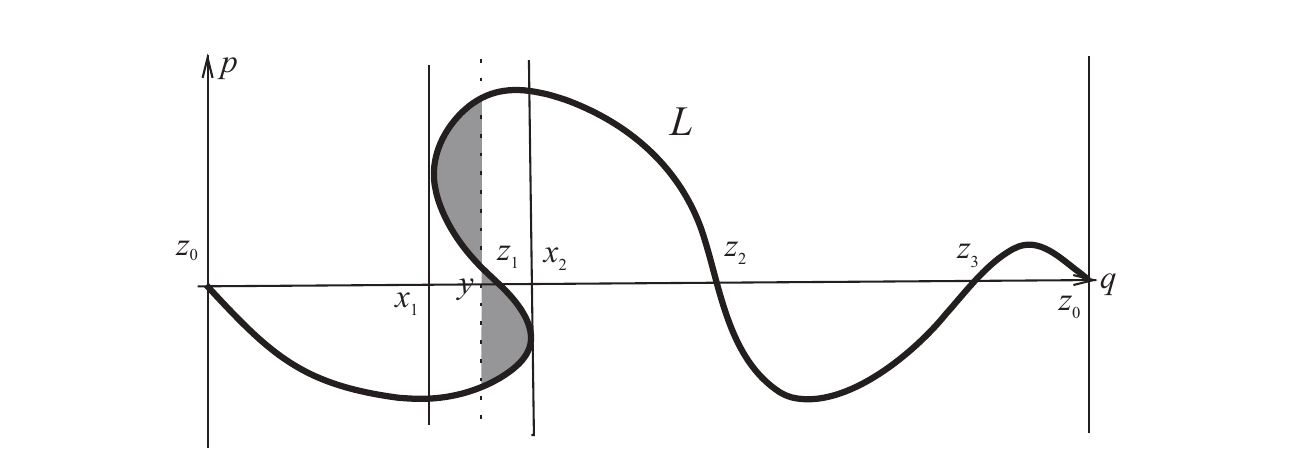
\includegraphics[width=0.9\textwidth]{chapters/ch12-cotangent-floer/figures/ch12-figure-12-1.png}
  \caption{\termMultisectionLagrangian{} $L$。}
  \label{fig:multisection-lagrangian}
\end{figure}

为了说明 $f_H$ 的含义，下面给出 $N=S^1$ 时的一个例子。

\begin{example}
\label{ex:wave-front-circle-multisection}
考虑\cref{fig:multisection-lagrangian}所示的拉格朗日子流形 $L\subset T^*S^1$。这里用 $z_i$ 表示 $L$ 与零截面的交点，用 $x_i$ 表示\termCaustic{}，并用 $y$ 表示图中两个阴影区域面积相等的点。相应的波前不难画成\cref{fig:wave-front-basic-phase}所示。

\begin{figure}[htbp]
  \centering
  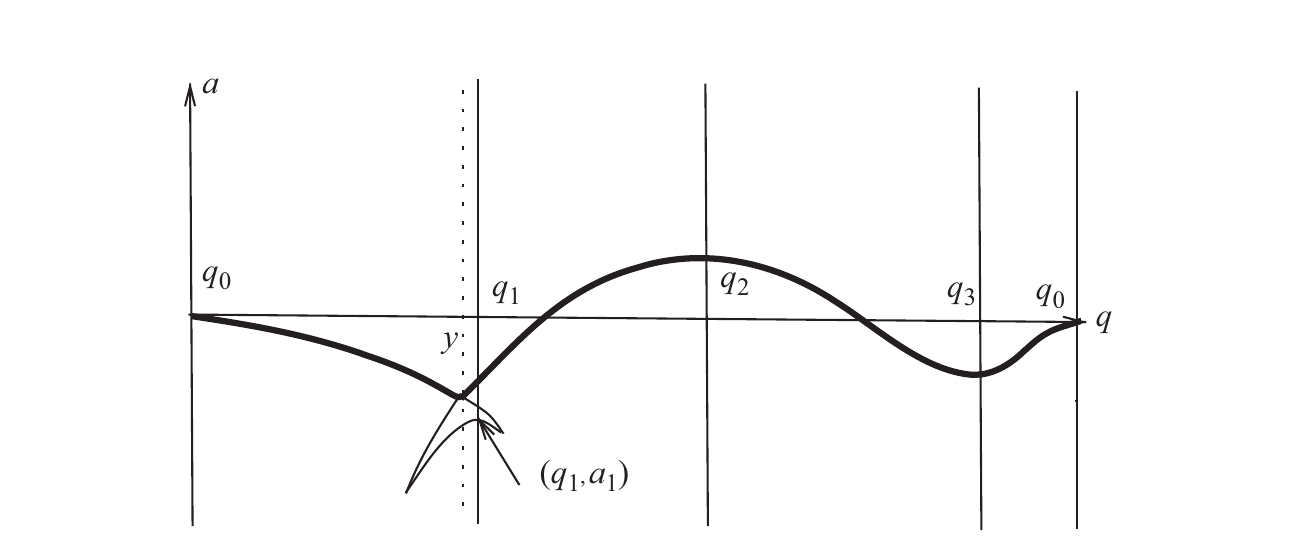
\includegraphics[width=0.88\textwidth]{chapters/ch12-cotangent-floer/figures/ch12-figure-12-2.png}
  \caption{$L$ 的\termWaveFront{}与 $f_H$ 的图。}
  \label{fig:wave-front-basic-phase}
\end{figure}

注意，$z_i$ 对应于作用量泛函的临界点，$x_i$ 对应于波前的\termCuspPoint{}，而 $y$ 对应于波前的两个不同分支相交之点。利用 $H\mapsto L$ 时基本相位函数 $f_H$ 的连续性，不难看出 $f_H$ 的图正是\cref{fig:wave-front-basic-phase}中的粗线。我们还要指出，数值
\[
  \min_{q\in N}f_H(q)
\]
\emph{并不是} $\mathcal A_H$ 的临界值，而是与波前交叉相伴的一个值。\footnote{译者注：原书末句把本节的 $f_H$ 突然写成此前未定义的 $F^H$；译文改回 $f_H$。}
\end{example}


\chapter{带冒泡的\personFloer{}复形的离壳框架}
\label{ch:off-shell-complex}

著名的\termRiemannRochFormula{}针对复向量丛截面上的 $\overline\partial$-算子，给出了由闭\personRiemann{}曲面出发的\termHolomorphicMap{}之\termModuliSpace{}的\termVirtualDimension{}公式。这个虚维数公式涉及该向量丛的\termFirstChernNumber{}。

本章回顾第一\personChern{}数之构造；一般而言，它通常称为\emph{\termMaslovIndex{}}。我们的叙述综合了 (Gr85)、(Oh95b) 与 (KL01) 中的处理。

\section{拉格朗日子空间与全实子空间}
\label{sec:lagrangian-versus-totally-real-subspaces}

\stfhIndex{I171}{Quanshizikongjian}{全实子空间（totally real subspace）}
为研究\termRiemannRochFormula{}的有边界版本，我们考虑 $\mathbb C^n$ 中（极大的）\emph{\termTotallyRealSubspace{}}。若实子空间 $V\subset\mathbb C^n$ 满足
\[
  V\cap iV=\{0\},
  \qquad
  \dim_{\mathbb R}V=n,
\]
则称 $V$ 是全实的。我们以 $\mathcal R(n)$ 表示所有全实子空间组成的集合。

任一全实子空间 $V$ 都可写成
\[
  V=A\cdot\mathbb R^n
\]
的形式，其中 $A\in GL(n,\mathbb C)$；而
$A_1\cdot\mathbb R^n=A_2\cdot\mathbb R^n$ 当且仅当
\begin{equation}
  A_2^{-1}A_1\in GL(n,\mathbb R).
\label{eq:totally-real-coset-condition}
\end{equation}
因此，全实子空间的集合 $\mathcal R(n)$ 是\termHomogeneousSpace{}：
\[
  \mathcal R(n)=GL(n,\mathbb C)/GL(n,\mathbb R).
\]
下面的引理是研究指标问题时一个有用的事实。其证明见 (Oh95b) 中的命题 4.4。

\begin{lemma}
\label{lem:totally-real-subspace-matrix-model}
考虑子集
\[
  \widetilde{\mathcal R}(n)
  :=\{D\in GL(n,\mathbb C)\mid D\overline D=I_n\},
\]
其中 $I_n$ 是单位矩阵。则映射
\[
  B:\mathcal R(n)\cong GL(n,\mathbb C)/GL(n,\mathbb R)
  \longrightarrow\widetilde{\mathcal R}(n);
  \qquad
  A\cdot\mathbb R^n\longmapsto A\overline A^{-1}
\]
是微分同胚。
\end{lemma}

\begin{proof}
考虑定义在 $GL(n,\mathbb C)$ 上的映射
\begin{equation}
  A\longmapsto A\overline A^{-1}.
\label{eq:matrix-conjugation-map}
\end{equation}
注意，任意形如 $A\overline A^{-1}$ 的矩阵 $D$ 都满足
$D\overline D=\operatorname{Id}_n$，所以这个映射的像落在
$\widetilde{\mathcal R}(n)$ 中。

方程~\eqref{eq:totally-real-coset-condition}等价于
\[
  A_1\overline A_1^{-1}=A_2\overline A_2^{-1}.
\]
这说明映射 $B$ 是良定义的。映射~\eqref{eq:matrix-conjugation-map}给出一一对应的证明留作练习。
\end{proof}

\begin{exercise}
\label{ex:matrix-conjugation-bijection}
证明映射~\eqref{eq:matrix-conjugation-map}给出一一对应。
\end{exercise}

下面考虑标准辛向量空间 $(\mathbb R^{2n},\omega_0)$，其中
\[
  \omega_0=\sum_{i=1}^n dx_i\wedge dy_i,
\]
这里使用典范坐标 $(x_1,\ldots,x_n,y_1,\ldots,y_n)$。以
\[
  \Lambda(n):=\mathcal L(\mathbb R^{2n},\omega_0)
\]
表示 $(\mathbb R^{2n},\omega_0)$ 的所有\termLagrangianSubspace{}组成的集合。若在 $\mathbb R^{2n}$ 上配备标准\termComplexMultiplication{}，并借映射
\[
  (x_i,y_i)\longmapsto z_i=x_i+\sqrt{-1}y_i
\]
将它与 $\mathbb C^n$ 等同，则每个拉格朗日子空间
$V\subset\mathbb C^n$ 都可以写成
\[
  V=A\cdot\mathbb R^n,
\]
其中复矩阵 $A\in U(n)$。这说明 $\Lambda(n)$ 是\termHomogeneousSpace{}：
\[
  \Lambda(n)\cong U(n)/O(n).
\]
特别地，这说明自然包含 $\Lambda(n)\hookrightarrow\mathcal R(n)$ 是\termHomotopyEquivalence{}。

(Ar67) 证明了
\[
  H^1(\Lambda(n),\mathbb Z)\cong\mathbb Z,
\]
而且 $\Lambda(n)$ 带有著名的\termCharacteristicClass{}
$\mu\in H^1(\Lambda(n),\mathbb Z)$，即\emph{\termMaslovClass{}} (Ar67)。它给每条给定的环路
$\gamma:S^1\to\Lambda(n)$ 指派如下整数\footnote{译者注：原书把 $\mu(\gamma)$ 写成 $\frac{1}{2\pi}\det^2(A)$；但右端按通常记号不是环路的整数值，也没有写出度数或辐角变化。译文照录原式，不自行重构。}：
\[
  \mu(\gamma)=\frac{1}{2\pi}\det^2(A).
\]
关于这个类的无坐标描述，参见第 3.2 节。此外，两条环路
$\gamma_1,\gamma_2$ 同伦，当且仅当
$\mu(\gamma_1)=\mu(\gamma_2)$。而且，只要双线性形式
$\omega_0(\,\cdot\,,J_0\,\cdot\,)$ 保持为\emph{正}，$\mu(\gamma)$ 的值就不依赖于 $\mathbb R^{2n}$ 与 $\mathbb C^n$ 的等同；这里 $J_0$ 是与 $\mathbb C^n$ 上复乘法相伴的殆复结构。

注意，当 $A$ 是\termUnitaryMatrix{}时，
$\overline A^{-1}=A^{\mathsf T}$，其中 $A^{\mathsf T}$ 是 $A$ 的转置。因此，由\cref{lem:totally-real-subspace-matrix-model}得到下面的推论。

\begin{corollary}
\label{cor:symmetric-unitary-model-lagrangian-grassmannian}
以 $\widetilde\Lambda(n)\subset\widetilde{\mathcal R}(n)$ 表示 $B$ 限制到
$\Lambda(n)\subset\mathcal R(n)$ 后的像，即
\begin{equation}
  \widetilde\Lambda(n)
  :=\{D\in U(n)\mid D=D^{\mathsf T}\},
\label{eq:symmetric-unitary-matrices}
\end{equation}
也就是\termSymmetricUnitaryMatrix{}组成的集合。则 $B$ 在 $\Lambda(n)$ 上的限制给出一个微分同胚。
\end{corollary}

下面把\termMaslovIndex{}推广到全实子空间的环路上；限制到
$\Lambda(n)$ 中的环路时，它就是马斯洛夫指标。

\begin{definition}[广义马斯洛夫指标]
\label{def:generalized-maslov-index}
设 $\gamma:S^1\to\mathcal R(n)$ 是一条环路。\termGeneralizedMaslovIndex{}
$\mu(\gamma)$ 定义为映射
\[
  \det\circ B\circ\gamma:S^1\longrightarrow\mathbb C\setminus\{0\}
\]
的\termWindingNumber{}。
\end{definition}

\section{丛对及其马斯洛夫指标}
\label{sec:bundle-pair-maslov-index}

设 $\Sigma$ 是带边界 $\partial\Sigma$ 的定向紧曲面。以 $g$ 表示
$\Sigma$ 的亏格，以 $h$ 表示 $\partial\Sigma$ 的连通分支数。

\subsection{复向量丛情形}
\label{subsec:complex-vector-bundle-pairs}

考虑复向量丛 $E\to\Sigma$。注意，若 $\partial\Sigma\ne\varnothing$，则
$\Sigma$ 上的任意复向量丛 $E\to\Sigma$ 在拓扑上都是平凡的。

\stfhSubIndex{I048}{Congdui}{丛对（bundle pair）}{Fu}{复丛对（complex bundle pair）}
\begin{definition}
\label{def:complex-bundle-pair}
一个\termComplexBundlePair{} $(E,\lambda)$ 是复向量丛 $E\to\Sigma$ 连同
$E|_{\partial\Sigma}$ 的一个实子丛 $\lambda\to\partial\Sigma$，并配备同构
\begin{equation}
  E|_{\partial\Sigma}\cong\lambda\otimes\mathbb C.
\label{eq:complex-bundle-boundary-complexification}
\end{equation}
等价地，复丛对是复向量丛 $E\to\Sigma$ 连同
$E_{\mathbb R}|_{\partial\Sigma}\to\partial\Sigma$ 的一个\termTotallyRealSubbundle{}
$\lambda\subset E_{\mathbb R}|_{\partial\Sigma}$；
这里 $E_{\mathbb R}$ 是丛 $E$ 的实化。
\end{definition}

固定一个\termTrivialization{}
\[
  \Phi:E\longrightarrow\Sigma\times\mathbb C^n,
\]
并设 $R_1,\ldots,R_h$ 是 $\partial\Sigma$ 的连通分支，各自带有从
$\Sigma$ 诱导的\termBoundaryOrientation{}。由给定的同构
$E|_{\partial\Sigma}\cong\lambda\otimes\mathbb C$，
$\Phi(\lambda|_{R_i})$ 给出环路
\[
  \gamma_{\Phi,i}:S^1\longrightarrow\mathcal R(n).
\]
令 $\mu(\Phi,R_i)=\mu(\gamma_{\Phi,i})$，便得到下面的命题。

\begin{proposition}
\label{prop:complex-bundle-pair-index-trivialization}
设 $(E,\lambda)$ 是定向紧曲面 $\Sigma$ 上秩为 $n$ 的复丛对。则
\[
  \sum_{i=1}^h\mu(\Phi,R_i)
\]
不依赖于平凡化 $\Phi:E\to\Sigma\times\mathbb C^n$ 的选取。\footnote{译者注：原书把求和指标写成 $j$，被求和项却仍为 $R_i$；译文统一为 $i$。}
\end{proposition}

\begin{proof}
设 $\Phi_1,\Phi_2$ 是 $E$ 的两个平凡化。于是
\[
  \Phi_2\circ\Phi_1^{-1}:
  \Sigma\times\mathbb C^n\longrightarrow\Sigma\times\mathbb C^n
\]
由 $(x,v)\mapsto(x,g(x)v)$ 给出，其中
\[
  g:\Sigma\longrightarrow GL(n,\mathbb C).
\]
由 $\gamma_{\Phi,i}$ 的定义\footnote{译者注：原书把第一条矩阵恒等式的左端写成
$g\overline g^{-1}\cdot B\circ\gamma_{\Phi_1,i}$，并在随后的度数公式中省去
$B\circ\gamma_{\Phi_j,i}$ 前的 $\det$，还把每个分支上的限制 $|_{R_i}$
写成 $|_{\partial\Sigma}$。译文依 $B(A\mathbb R^n)=A\overline A^{-1}$
及本节对 $\mu(\Phi,R_i)$ 的定义补正这些对象。}，
\[
  g\,(B\circ\gamma_{\Phi_1,i})\,\overline g^{-1}
  =B\circ\gamma_{\Phi_2,i}.
\]
因此
\[
\begin{aligned}
  \deg(\det\circ B\circ\gamma_{\Phi_2,i})
  ={}&
  \deg\left(\left.\det(g\overline g^{-1})\right|_{R_i}\right)
  +\deg(\det\circ B\circ\gamma_{\Phi_1,i}),
\end{aligned}
\]
亦即
\[
  \mu(\Phi_2,R_i)-\mu(\Phi_1,R_i)
  =\deg\left(\left.\det(g\overline g^{-1})\right|_{R_i}\right).
\]
另一方面，因为 $\partial\Sigma=\coprod_iR_i$，而映射
\[
  \left.\det(g\overline g^{-1})\right|_{\partial\Sigma}:
  \partial\Sigma\longrightarrow S^1
\]
显然可以延拓到 $\Sigma$，所以由度数的\termCobordismInvariance{}，
\[
  \sum_{i=1}^h
  \deg\left(\left.\det(g\overline g^{-1})\right|_{R_i}\right)=0.
\]
证明完成。
\end{proof}

\cref{prop:complex-bundle-pair-index-trivialization}说明下面的定义是良定义的。

\stfhIndex{I124}{Masiluofuzhibiao}{马斯洛夫指标（Maslov index）}
\begin{definition}
\label{def:complex-bundle-pair-maslov-index}
\termBundlePair{} $(E,\lambda)$ 的\termMaslovIndex{}定义为
\begin{equation}
  \mu(E,\lambda)=\sum_{i=1}^h\mu(\Phi,R_i),
\label{eq:complex-bundle-pair-maslov-index}
\end{equation}
其中 $\Phi:E\to\Sigma\times\mathbb C^n$ 是某个（因而任意）平凡化。
\end{definition}

\subsection{辛向量丛情形}
\label{subsec:symplectic-vector-bundle-pairs}

考虑一个\termSymplecticVectorBundle{} $E\to\Sigma$，也就是说，假设每条纤维
$E_x$ 都带有一个随 $x\in\Sigma$ 光滑变化的辛内积 $\omega_x$。
同样，若 $h>0$，则 $\Sigma$ 上的任意辛向量丛都是辛平凡的。固定一个\termSymplecticTrivialization{}
\[
  \Psi:E\longrightarrow\Sigma\times(\mathbb R^{2n},\omega_0).
\]

\stfhSubIndex{I049}{Congdui}{丛对（bundle pair）}{Xin}{辛丛对（symplectic bundle pair）}
\begin{definition}
\label{def:symplectic-bundle-pair}
一个\termSymplecticBundlePair{}是对子 $(E,\lambda)$，其中
$E\to\Sigma$ 是辛向量丛，而 $\lambda\to\partial\Sigma$ 是
$E|_{\partial\Sigma}$ 的一个\termLagrangianSubbundle{}。
\end{definition}

回忆，$\mathbb C^n$ 的任意拉格朗日子空间之\termComplexification{}都典范同构于
$\mathbb C^n$。把这与\cref{def:complex-bundle-pair}比较。与复情形一样，限制
$\Psi(\lambda|_{R_i})$ 给出环路
\[
  \gamma_{\Psi,i}:S^1\longrightarrow\Lambda(n).
\]
记 $\mu(\Psi,R_i)=\mu(\gamma_{\Psi,i})$。于是有下述命题。

\begin{proposition}
\label{prop:symplectic-bundle-pair-index-trivialization}
设 $(E,\lambda)$ 是定向紧曲面 $\Sigma$ 上的辛丛对。则
\[
  \sum_{i=1}^h\mu(\Psi,R_i)
\]
不依赖于辛平凡化
$\Psi:E\to\Sigma\times(\mathbb R^{2n},\omega_0)$ 的选取。\footnote{译者注：原书再次把求和指标写成 $j$、被求和项写成 $R_i$；并把平凡化的靶写成 $E\times\mathbb C^n$。译文分别统一为 $i$ 及本小节已经固定的 $\Sigma\times(\mathbb R^{2n},\omega_0)$。}
\end{proposition}

\begin{proof}
设
\[
  \Psi_1,\Psi_2:
  E\longrightarrow\Sigma\times(\mathbb R^{2n},\omega_0)
\]
是两个辛平凡化\footnote{译者注：原书在本证明中把两个辛平凡化的靶及过渡映射的定义域、值域都只写成
$(\mathbb R^{2n},\omega_0)$，但下一行的赋值仍使用基点 $x$。译文补回
$\Sigma\times(\mathbb R^{2n},\omega_0)$。}。映射
\[
  \Psi_2\circ\Psi_1^{-1}:
  \Sigma\times(\mathbb R^{2n},\omega_0)
  \longrightarrow
  \Sigma\times(\mathbb R^{2n},\omega_0)
\]
由 $(x,v)\mapsto(x,g(x)v)$ 给出，其中
\[
  g:\Sigma\longrightarrow\operatorname{Sp}(2n,\mathbb R).
\]
把 $\operatorname{Sp}(2n,\mathbb R)$ 在 $\Lambda(n)$ 上的自然作用写成
$g\cdot V$。于是
\[
  g(x)\gamma_{\Psi_1,i}(x)=\gamma_{\Psi_2,i}(x),
  \qquad x\in R_i.
\]

因为 $\mathbb C^n$ 的任意拉格朗日子空间关于标准复乘法都是全实的，而且\termGeneralizedMaslovIndex{}在 $\mathcal R(n)$ 中的同伦下不变，所以这个恒等式给出
\[
  \mu(\Psi_2,R_i)=\mu(\Psi_1,R_i)+2\deg(g|_{R_i}),
\]
其中 $\deg(g|_{R_i})$ 是第 2.2.2 节中定义的环路
\[
  g|_{R_i}:S^1\longrightarrow\operatorname{Sp}(2n,\mathbb R)
\]
的度数。因为
\[
  g|_{\partial\Sigma}=\coprod_{i=1}^h g|_{R_i},
\]
再次得到
\[
  \sum_{i=1}^h\deg(g|_{R_i})=0,
\]
证明即告完成。
\end{proof}

这个命题使我们能够定义辛丛对 $(E,\lambda)$ 的马斯洛夫指标
$\mu(E,\lambda)$。

\begin{definition}
\label{def:symplectic-bundle-pair-maslov-index}
辛丛对 $(E,\lambda)$ 的马斯洛夫指标定义为
\begin{equation}
  \mu(E,\lambda)=\sum_{i=1}^h\mu(\Psi,R_i),
\label{eq:symplectic-bundle-pair-maslov-index}
\end{equation}
其中 $\Psi:E\to\Sigma\times(\mathbb R^{2n},\omega_0)$ 是某个（因而任意）
辛平凡化。\footnote{译者注：原书此处沿用复丛对定义中的 $\Phi$ 与
$\Sigma\times\mathbb C^n$，但本小节此前始终以 $\Psi$ 表示取值于
$\Sigma\times(\mathbb R^{2n},\omega_0)$ 的辛平凡化；译文依此统一。}
\end{definition}

不难证明 $\mu(E,\lambda)$ 的\termHomotopyInvariance{}。事实上，它满足一个更强的不变性；现在来表述这一点。

设 $(E_1,\lambda_1)$、$(E_2,\lambda_2)$ 分别是 $\Sigma_1$、$\Sigma_2$
上的辛丛对。\footnote{译者注：原书此处先写 $(E_0,\lambda_0)$、
$(E_1,\lambda_1)$，随后在命题中混用下标 $0,1,2$ 以及未定义的
$\Sigma_0,E_2,\lambda_2$。译文依命题结论与配边的两个边界分支统一为下标
$1,2$。}

\begin{proposition}
\label{prop:maslov-cobordism-invariance}
假设实向量丛
\[
  \lambda_1|_{\partial\Sigma_1}
  \sqcup
  \lambda_2|_{\partial\Sigma_2}
\]
可以延拓为\termOrientedCobordism{} $\Sigma_{12}$ 上的实向量丛
$\lambda_{12}\to\Sigma_{12}$，其中
\[
  \partial\Sigma_{12}
  =-\partial\Sigma_1\sqcup\partial\Sigma_2,
\]
并且 $\lambda_{12}$ 嵌入辛向量丛 $E_{12}\to\Sigma_{12}$，成为一个拉格朗日子丛；其在边界 $\partial\Sigma_{12}$ 上限制为丛对
\[
  (E_1,\lambda_1)|_{\partial\Sigma_1}
  \sqcup
  (E_2,\lambda_2)|_{\partial\Sigma_2}.
\]
则
\[
  \mu(E_1,\lambda_1)=\mu(E_2,\lambda_2).
\]
\end{proposition}

\begin{proof}
任选 $E_{12}\to\Sigma_{12}$ 的一个平凡化
\[
  \Phi_{12}:E_{12}
  \longrightarrow
  \Sigma_{12}\times(\mathbb R^{2n},\omega_0).
\]
它显然定义了 $E_1$ 和 $E_2$ 的平凡化。在这个平凡化中计算
$\mu(E_i,\lambda_i)$（$i=1,2$）以及 $\mu(E_{12},\lambda_{12})$，结论随即成立。
\end{proof}

我们把这个命题的陈述称为 $\mu(E,\lambda)$ 的\termCobordismInvariance{}。
显然，这个命题蕴含 $\mu(E,\lambda)$ 的同伦不变性。

现在设 $L\subset(M,\omega)$ 是拉格朗日子流形，并考虑光滑映射
\[
  w:(\Sigma,\partial\Sigma)\longrightarrow(M,L).
\]
以 $\partial w:\partial\Sigma\to L$ 表示限制 $w|_{\partial\Sigma}$。于是
$(w,\partial w)$ 诱导一个典范丛对
\[
  E=w^*TM,
  \qquad
  \lambda=(\partial w)^*TL.
\]

\begin{definition}
\label{def:maslov-index-map}
设 $w$ 如上。$w$ 的马斯洛夫指标记为 $\mu_L(w)$，定义为
\[
  \mu_L(w)=\mu\bigl(w^*TM,(\partial w)^*TL\bigr).
\]
\end{definition}

$\mu(E,\lambda)$ 的同伦不变性立即推出映射 $w$ 的 $\mu_L(w)$ 具有同伦不变性。

\section{多边形映射的马斯洛夫指标}
\label{sec:maslov-indices-polygonal-maps}

\stfhSubIndex{I125}{Masiluofuzhibiao}{马斯洛夫指标（Maslov index）}{Duobianxingyingshedezhibiao}{多边形映射的指标（of polygonal map）}
本节依照 (FOOO10a) 中的叙述，为\termPolygonalMap{}指派一个\termTopologicalIndex{}。

首先说明如何利用命题 3.2.14，把一个自然丛对关联给每个附着于\termTransversalLagrangianChain{}的\emph{多边形映射}。

考虑带有一组\termMarkedPoint{}
\[
  \{u_0,u_1,\ldots,u_k\}\subset\partial D^2
\]
的圆盘 $\Sigma=D^2$。把（边界）\termPuncturedDisc{}记为
\[
  \dot\Sigma=D^2\setminus\{u_i\}_{0\le i\le k}.
\]
对 $i=0,\ldots,k$，固定 $u_i$ 在 $\Sigma$ 中的一个小闭邻域
$U_i$，使各 $U_i$ 两两不交\footnote{译者注：原书写成“使各点
$u_i$ 互不相交”；这些标记点本来已经互异，而这里需要选取为两两不交的是
邻域 $U_i$。译文依此补正。}，并在每个邻域上配备一个\termConformalIsomorphism{}
\[
  U_i\setminus\{u_i\}\longrightarrow(-\infty,0]\times[0,1].
\]

令
\[
  \mathcal L=(L_0,L_1,\ldots,L_k)
\]
是拉格朗日子流形 $L_i$（$i=0,\ldots,k$）的一个有序
$(k+1)$-元组。

\begin{definition}
\label{def:transversal-lagrangian-chain}
若 $\mathcal L$ 两两横截，并且对任意互异的三元组 $i,j,\ell$ 都有
\[
  L_i\cap L_j\cap L_\ell=\varnothing,
\]
则称 $\mathcal L$ 为\termTransversalChain{}。称 $k+1$ 为该链的长度。
\end{definition}

现在考虑一条交点链
\[
  \vec p
  =\{p_{i(i+1)}\in L_i\cap L_{i+1}\mid i=0,\ldots,k\}
\]
以及一个光滑映射 $w:\dot\Sigma\to M$；它连续延拓到 $\Sigma$，并满足
\begin{equation}
  \lim_{z\to u_i}w(z)=p_{i(i+1)},
  \qquad
  w\bigl(\overline{u_i u_{i+1}}\bigr)\subset L_{i+1}.
\label{eq:polygonal-map-boundary-data}
\end{equation}
这里及下文的下标按模 $k+1$ 理解，即
$u_{k+1}=u_0$、$L_{k+1}=L_0$。\footnote{译者注：原书在
$i=k$ 时仍使用 $u_{i+1}$、$L_{i+1}$，却没有声明循环约定；译文将其明示。
此外，原书在\eqref{eq:polygonal-map-boundary-data}的第二个条件中写的是
$L_i$。但它令 $u_i$ 映到 $L_i\cap L_{i+1}$，且下一页起始终把 $u_i$
两侧的边界段分别配给 $L_i$ 与 $L_{i+1}$；译文依这套后续构造把此处补正为
$L_{i+1}$。}

\stfhIndex{I022}{00-pi2-l-p}{\stfhIndexPiTwoLMarkedP}
以
\[
  \pi_2(\mathcal L;\vec p)
\]
表示这类连续映射的同伦类集合，并以 $B$ 表示
$\pi_2(\mathcal L;\vec p)$ 的一个元素。接下来要相对于数据
$\mathcal L$、$\vec p$ 与 $B$，为这类映射 $w$ 指派一个拓扑指标。
考虑 $w^*TM$ 的一个\termSymplecticTrivialization{}：
\[
  w^*TM\cong
  \dot\Sigma\times(\mathbb R^{2n},\omega_0).
\]

在这个平凡化下，映射
\[
  \alpha_w:S^1=\partial\Sigma\longrightarrow\Lambda(n);
  \qquad
  t\longmapsto T_{w(t)}L_i
  \quad\text{若 }t\in\overline{u_{i-1}u_i}
\]
定义了一条\termPiecewiseSmoothPath{}；它在 $k+1$ 个点
$u_i\in\partial D^2$（$i=0,1,\ldots,k$）处不连续。\footnote{译者注：
原书把该映射的定义域写成 $S^1=\dot\Sigma$，但 $\dot\Sigma$ 是二维穿孔圆盘；
从分段条件 $t\in\overline{u_{i-1}u_i}$ 以及紧接着列出的不连续点可知，定义域应为
边界圆周 $\partial\Sigma$。译文依此补正。}
由横截性假设，$(\mathbb R^{2n},\omega_0)$ 中的两个拉格朗日子空间
$T_{w(u_i)}L_i$ 与 $T_{w(u_i)}L_{i+1}$\footnote{译者注：原书在此处的
第二个切空间以及下方路径端点中都把基点写成 $w(u_{i+1})$。然而横截对
$L_i,L_{i+1}$ 的共同交点是 $w(u_i)=p_{i(i+1)}$，而且随后选取的\personDarboux{}坐标卡也以该点为中心；译文两处均统一为 $w(u_i)$。}满足
\[
  T_{w(u_i)}L_i\cap T_{w(u_i)}L_{i+1}=\{0\}.
\]
从这些数据出发，我们将在适当构造的\termBorderedRiemannSurface{}
$\widehat{\dot\Sigma}$ 上关联出光滑\termSymplecticBundlePair{}
$(E_w,\lambda_w)$。

首先，对每个 $i=0,\ldots,k$，考虑辛向量空间
\[
  (S,\Omega)=\bigl(T_{w(u_i)}M,\omega_{w(u_i)}\bigr),
\]
并按照命题 3.2.14 选定一条光滑路径
\[
  \alpha_{i(i+1)}:[0,1]\longrightarrow\mathcal L(S,\Omega),
\]
使得
\[
  \alpha_{i(i+1)}(0)=T_{w(u_i)}L_i,
  \qquad
  \alpha_{i(i+1)}(1)=T_{w(u_i)}L_{i+1}.
\]

在每个 $p_{i(i+1)}\in L_i\cap L_{i+1}$ 处，都存在定义在
$V_i$ 上的\termDarbouxChart{}
\[
  \Phi_i:V_i\longrightarrow T_{p_{i(i+1)}}M,
\]
其中 $V_i$ 是 $p_{i(i+1)}$ 在 $M$ 中的一个邻域，并且\footnote{译者注：
原书在条件 (1) 以及条件 (3) 两个等式的右端把 $\Phi_i$ 误写成了 $\Phi$；
译文补回下标 $i$。}
\begin{enumerate}[label=(\arabic*)]
  \item $\Phi_i(p_{i(i+1)})=0\in T_{p_{i(i+1)}}M$；
  \item
  \[
    d\Phi_i(p_{i(i+1)}):
    T_{p_{i(i+1)}}M\longrightarrow T_{p_{i(i+1)}}M
  \]
  是恒等映射；
  \item
  \[
  \begin{aligned}
    \Phi_i(V_i\cap L_i)
      &=\Phi_i(V_i)\cap T_{p_{i(i+1)}}L_i,\\
    \Phi_i(V_i\cap L_{i+1})
      &=\Phi_i(V_i)\cap T_{p_{i(i+1)}}L_{i+1}.
  \end{aligned}
  \]
\end{enumerate}

\begin{exercise}
\label{ex:darboux-chart-transversal-pair}
证明这样的\personDarboux{}坐标卡存在。
\end{exercise}

于是，由\eqref{eq:polygonal-map-boundary-data}中的收敛性，可以把
$\dot\Sigma$ 完备化为紧致带边\personRiemann{}曲面\footnote{译者注：原书称非紧的
$\dot\Sigma$ 为“紧致带边\personRiemann{}曲面”，又说把它“分解”为随后才定义的
$\widehat{\dot\Sigma}$，并在端部等同中交替使用 $U_i$ 与
$U_i\setminus\{u_i\}$。译文依本段的构造改写为把 $\dot\Sigma$ 完备化，并在涉及
半无限带时明确删去穿孔。}
\[
  \widehat{\dot\Sigma}
  :=\dot\Sigma\cup\bigcup_i\widehat U_i,
\]
其中 $w(U_i)\subset V_i$。令
\[
  \widehat U_i\cong[-\infty,0]\times[0,1]
\]
为
\[
  (-\infty,0]\times[0,1]
  \cong U_i\setminus\{u_i\}
\]
的自然完备化（$i=0,\ldots,k$）。称这个并为 $\dot\Sigma$ 沿其各穿孔、
关于端部共形坐标卡
\[
  U_i\setminus\{u_i\}\cong(-\infty,0]\times[0,1]
\]
\stfhIndex{I164}{Shibaopo}{实爆破（real blow-up）}
所作的\emph{\termRealBlowUp{}}。

对 $p_{i(i+1)}$ 的邻域上给定的\personDarboux{}坐标卡 $\Phi_i$，映射
$\Phi_i\circ w$ 满足
\begin{equation}
  d\Phi_i\bigl(T_{w(\tau,0)}L_i\bigr)
    \equiv T_{p_{i(i+1)}}L_i,
  \qquad
  d\Phi_i\bigl(T_{w(\tau,1)}L_{i+1}\bigr)
    \equiv T_{p_{i(i+1)}}L_{i+1}.
\label{eq:darboux-end-trivialization}
\end{equation}
而且\footnote{译者注：原书在这里写成
$\Phi_i\circ w(\infty,t)\equiv p_{i(i+1)}$；但本段采用的是
$[-\infty,0]\times[0,1]$，且 $\Phi_i(p_{i(i+1)})=0$。译文相应补正端部符号与
坐标值。}
\[
  \Phi_i\circ w(-\infty,t)\equiv0.
\]
把 $w$ 到 $\widehat{\dot\Sigma}$ 的连续延拓记为
\[
  \widehat w:\widehat{\dot\Sigma}\longrightarrow M.
\]

\begin{lemma}
\label{lem:polygonal-pullback-extension}
$\dot\Sigma$ 上的拉回丛\footnote{译者注：原书在引理陈述中把主丛写成
$(\Phi\circ\widehat w)^*M$，把边界丛写成
$(\partial_j(\Phi\circ\widehat w))^*TL_j$，证明中又把 $w^*TM$ 写成
$w^*M$；这些写法混淆了拉回丛、\personDarboux{}坐标映射及其导数。原证明明确说平凡化由
$d\Phi_i$ 给出，译文据此统一为相应的切丛拉回，并以
$\widehat U_i$ 表示包含新增端边的完备化邻域。}$w^*TM$ 可以光滑延拓为
$\widehat w^*TM$。在 $\widehat U_i$ 上，这一延拓具有典范平凡化
\[
\begin{aligned}
  &\bigl(\widehat w^*TM;
    (\partial_i\widehat w)^*TL_i,
    (\partial_{i+1}\widehat w)^*TL_{i+1}\bigr)
    \big|_{\widehat U_i}\\
  &\qquad\cong
  (\widehat U_i;\partial_0\widehat U_i,\partial_1\widehat U_i)
  \times
  \bigl(T_{p_{i(i+1)}}M;
    T_{p_{i(i+1)}}L_i,T_{p_{i(i+1)}}L_{i+1}\bigr),
\end{aligned}
\]
其中 $\partial_i\widehat w$ 与 $\partial_{i+1}\widehat w$ 表示
$\widehat w$ 在 $\widehat U_i$ 两条边界边上的相应限制。
\end{lemma}

\begin{proof}
由\eqref{eq:darboux-end-trivialization}，$w^*TM$ 有一个平凡化，使得三元组
\[
  \bigl(w^*TM;(\partial_iw)^*TL_i,
    (\partial_{i+1}w)^*TL_{i+1}\bigr)
\]
限制到 $U_i\setminus\{u_i\}$ 后，在导数 $d\Phi_i$ 下映到平凡丛
\[
  (U_i\setminus\{u_i\};\partial_0U_i,\partial_1U_i)
  \times
  \bigl(T_{p_{i(i+1)}}M;
    T_{p_{i(i+1)}}L_i,T_{p_{i(i+1)}}L_{i+1}\bigr).
\]
引理立即由此得证。
\end{proof}

现在，我们已把拉回丛
\[
  w^*TM\longrightarrow\dot\Sigma
\]
光滑延拓为
\[
  \widehat w^*TM\longrightarrow\widehat{\dot\Sigma}.
\]
把相应的辛向量丛记为
\[
  E_w=\widehat w^*TM.
\]

接下来描述一个拉格朗日子丛\footnote{译者注：原书在这一段的三次边界记号中分别写成
$\partial\widehat{\dot\Sigma}$、$\partial\widehat\Sigma$ 以及
$\partial\dot{\widehat\Sigma}$；译文统一为本段已经构造的
$\partial\widehat{\dot\Sigma}$。}
\[
  \lambda\subset E_w|_{\partial\widehat{\dot\Sigma}}.
\]
在 $\dot\Sigma$ 的穿孔 $u_i$ 处，把路径
\[
  \alpha_{i(i+1)}:[0,1]\longrightarrow
  \Lambda\bigl(T_{w(u_i)}M\bigr)
\]
插入 $\{-\infty\}\times[0,1]$，放在两个\termGaussMap{}
\[
  \alpha_w|_{\overline{u_{i-1}u_i}}
  \quad\text{与}\quad
  \alpha_w|_{\overline{u_i u_{i+1}}}
\]
之间；这样就得到 $E_w|_{\partial\widehat{\dot\Sigma}}$ 的一个\termLagrangianSubbundle{}
\[
  \lambda_w\longrightarrow\partial\widehat{\dot\Sigma}.
\]

\stfhSubIndex{I126}{Masiluofuzhibiao}{马斯洛夫指标（Maslov index）}{DuobianxingMasiluofuzhibiao}{多边形马斯洛夫指标（polygonal Maslov index）}
\begin{definition}
\label{def:polygonal-maslov-index}
定义\termPolygonalMaslovIndex{}，记作 $\mu(w;\mathcal L,\vec p)$，为马斯洛夫指标
\[
  \mu(w;\mathcal L,\vec p)=\mu(E_w,\lambda_w).
\]
\end{definition}

当拉格朗日链 $\mathcal L$ 的长度为二，即 $k=1$ 时，这个指标以一种自然方式
与拉格朗日对子 $(L_0,L_1)$ 的\termMaslovViterboIndex{} (Vi88) 相关；我们将在
定义 13.6.2 中给出这种关系。

\begin{exercise}
\label{ex:maslov-viterbo-relation}
找出马斯洛夫指标与\personMaslov{}--\personViterbo{}指标之间的确切关系。
\end{exercise}

\begin{proposition}
\label{prop:polygonal-maslov-homotopy-invariance}
$\mu(w;\mathcal L,\vec p)$ 只依赖于同伦类
$[w]\in\pi_2(\mathcal L,\vec p)$ 以及路径 $\alpha_{i(i+1)}$ 的选取。
对 $B=[w]$，把相应的共同指标记为
$\mu(\mathcal L,\vec p;B)$。
\end{proposition}

\begin{proof}
设 $w_0,w_1$ 是定义在
\[
  \dot\Sigma=D^2\setminus\{u_i\}_{i=0,\ldots,k}
\]
上、附着于数据 $(\mathcal L,\vec p)$ 的两个相互同伦的多边形映射
\footnote{译者注：原书把这组穿孔的下标范围排成
$i=0,\mathord\cdot,k$；译文按本节此前的范围补为 $i=0,\ldots,k$。}
。它们之间的光滑同伦 $\{w_s\}_{0\le s\le1}$ 诱导一族辛向量丛
$w_s^*TM$。由于 $[0,1]$ 紧，可以找到 $u_i$ 的一个公共邻域 $U_i$，使
$w_s^*TM$ 被 $\Phi$ 平凡化，并且对所有 $s\in[0,1]$ 都有
\[
\begin{aligned}
  d\Phi:
  &\bigl(w_s^*TM|_{U_i};
    (\partial w_s)^*TL_i,(\partial w_s)^*TL_{i+1}\bigr)\\
  &\quad\longrightarrow
  (U_i;\partial_0U_i,\partial_1U_i)
  \times
  \bigl(T_{w(u_i)}M;T_{w(u_i)}L_i,T_{w(u_i)}L_{i+1}\bigr).
\end{aligned}
\]
我们用同一条路径 $\alpha_{i(i+1)}$ 填入线段\footnote{译者注：原书此处改写为
$\{\infty_i\}\times[0,1]\subset[0,\infty]\times[0,1]$，与本节此前固定的
$[-\infty,0]\times[0,1]$ 端部坐标相反；译文统一回负无穷端。}
\[
  \{-\infty_i\}\times[0,1]
  \subset[-\infty,0]\times[0,1]
  \cong\widehat U_i.
\]
再把上面的平凡化 $d\Phi$ 延拓到 $D^2$ 的其余部分，便得到丛对
$(E_{w_s},\lambda_{w_s})$ 的一个同伦。由丛对马斯洛夫指标的同伦不变性，得到
\[
  \mu(E_0,\lambda_0)=\mu(E_1,\lambda_1),
\]
证明完成。
\end{proof}

这个拓扑指标是计算构造\termFukayaCategory{}时出现的
$\overline\partial$-算子之线性化的\termFredholmIndex{}的基础。（参见
(FOOO10a)。）

\section{\personNovikov{}覆盖与\personNovikov{}环}
\label{sec:novikov-covering-ring}

设 $(L_0,L_1)$ 是 $(M,\omega)$ 中一对相互横截的紧拉格朗日子流形。
\footnote{译者注：原书在本句中先称 $L_0,L_1$ 连通，下一句却特意声明此时不假设
它们连通；下一页还先用基准道路选出各自的连通分支，才说从此可以假设二者连通。
译文依这段论证删去本句中提前出现的“连通”。}
需要指出，此刻我们并\emph{不}假设拉格朗日子流形是连通的。

考虑道路空间
\[
  \Omega=\Omega(L_0,L_1)
  =\{\ell:[0,1]\longrightarrow M
    \mid \ell(0)\in L_0,\ \ell(1)\in L_1\}.
\]
\footnote{译者注：原书把道路 $\ell$ 的值域写成未定义的 $P$；本节的环境辛流形
始终为 $M$，译文依此补正。}
\stfhIndex{I026}{Zuoyongyixingshi}{作用 1-形式（action one-form）}
在 $\Omega$ 上定义一个 $1$-形式（\emph{作用 $1$-形式}）$\alpha$：
\begin{equation}
  \alpha(\ell)(\xi)
  =\int_0^1\omega\bigl(\dot\ell(t),\xi(t)\bigr)\,dt,
\label{eq:lagrangian-action-one-form}
\end{equation}
其中 $\xi\in T_\ell\Omega$；由推论 3.8.4 可知，它是一个“\emph{闭} $1$-形式”。

$\Omega(L_0,L_1)$ 并不连通，但它有可数多个连通分支。以后研究\personFloer{}模空间时，
我们总是在 $\Omega(L_0,L_1)$ 的某个固定连通分支上工作。选取一条\emph{\termBasePath{}} $\ell_0$，便指定了这个分支；把相应分支记为
\[
  \Omega(L_0,L_1;\ell_0)\subset\Omega(L_0,L_1).
\]

基准道路 $\ell_0$ 的始点和终点
\[
  x_0=\ell_0(0)\in L_0,
  \qquad
  x_1=\ell_0(1)\in L_1
\]
自动分别从 $L_0,L_1$ 中选出一个连通分支。于是
$\Omega(L_0,L_1;\ell_0)$ 无非就是这两个相应连通分支之间的道路空间。
因此，除非另有说明，从现在起\emph{我们总是假设 $L_0,L_1$ 连通}。

\stfhIndex{I138}{Nuoweikefufugai}{诺维科夫覆盖（Novikov covering）}
接下来描述一个覆盖空间，称为 $\Omega(L_0,L_1)$ 的分支
$\Omega(L_0,L_1;\ell_0)$ 的\emph{\termNovikovCovering{}}。我们先描述
$\Omega(L_0,L_1;\ell_0)$ 的\termUniversalCoveringSpace{}。考虑所有满足下列
边界条件的对子 $(\ell,w)$：
\begin{align}
  w(0,\mathord\cdot)&=\ell_0,
  &w(1,\mathord\cdot)&=\ell,
  \label{eq:novikov-filling-path-ends}\\
  w(s,0)&\in L_0,
  &w(s,1)&\in L_1
  \quad\text{对所有 }s\in[0,1].
  \label{eq:novikov-filling-boundary}
\end{align}
把 $w$ 看成 $\Omega(L_0,L_1;\ell_0)$ 中一条从 $\ell_0$ 到 $\ell$ 的连续道路，
则 $\Omega(L_0,L_1;\ell_0)$ 的万有覆盖空间在 $\ell$ 上的纤维，可以由 $w$
相对于两端 $s=0,1$ 的道路同伦类集合表示。\footnote{译者注：原书此处写成
“from $\ell_0$ and $\ell$”；按万有覆盖的道路模型以及本句紧接的端点条件，应为
“从 $\ell_0$ 到 $\ell$”。}
把 $\Omega(L_0,L_1;\ell_0)$ 中满足
\eqref{eq:novikov-filling-path-ends}的 $w$ 的这个同伦类记为 $[\ell,w]$。

现在用另一个比同伦更弱的等价关系对上述万有覆盖空间取商，由此定义
$\Omega(L_0,L_1;\ell_0)$ 的一个较小覆盖空间。这类似于辛流形
$(M,\omega)$ 的可缩环路空间的\personNovikov{}覆盖空间；我们将在第 4 部分研究后者。

注意，若给定两个对子 $(\ell,w)$ 与 $(\ell,w')$，其公共道路
$\ell\in\Omega(L_0,L_1;\ell_0)$，则拼接
\[
  \overline w\#w':[0,1]\times[0,1]\longrightarrow M
\]
定义了一个环路
\[
  c:S^1\longrightarrow\Omega(L_0,L_1;\ell_0).
\]
可以把这个环路视为一个\termAnnularMap{}
\[
  C:S^1\times[0,1]\longrightarrow M,
\]
它满足边界条件
\begin{equation}
  C(s,0)\in L_0,
  \qquad
  C(s,1)\in L_1.
\label{eq:annular-map-lagrangian-boundary}
\end{equation}
显然，$C$ 的\termSymplecticArea{}记为
\begin{equation}
  I_\omega(C)=\int_C\omega,
\label{eq:annular-symplectic-area}
\end{equation}
它只依赖于满足\eqref{eq:annular-map-lagrangian-boundary}的 $C$ 的同伦类，
因而定义了一个同态，记为
\[
  I_\omega:
  \pi_1\bigl(\Omega(L_0,L_1;\ell_0)\bigr)
  \longrightarrow\mathbb R.
\]

接下来注意，对满足\eqref{eq:annular-map-lagrangian-boundary}的映射
$C:S^1\times[0,1]\to M$，可以关联一个辛丛对 $(E_C,\lambda_C)$：
\[
  E_C=C^*TM,
  \qquad
  \lambda_C=R_0^*TL_0\sqcup R_1^*TL_1,
\]
其中 $R_i:S^1\to L_i$ 是映射
\[
  R_i(s)=C(s,i),
  \qquad i=0,1.
\]
这使我们能够定义另一个同态
\[
  I_\mu:
  \pi_1\bigl(\Omega(L_0,L_1;\ell_0),\ell_0\bigr)
  \longrightarrow\mathbb Z;
  \qquad
  I_\mu(c)=\mu(E_C,\lambda_C),
\]
其中 $\mu(E_C,\lambda_C)$ 是丛对 $(E_C,\lambda_C)$ 的马斯洛夫指标。
\footnote{译者注：原书在 $I_\mu$ 的定义域中突然把已经固定的分支记号
$\Omega(L_0,L_1;\ell_0)$ 改写成未定义的 $\Omega_{\ell_0}(L_0,L_1)$；译文统一
沿用前者。}

利用 $I_\mu$ 与 $I_\omega$\footnote{译者注：原书在此把同态 $I_\omega$
称为“辛形式”；译文按上文已经给出的类型只写其记号。}，在所有满足
\eqref{eq:novikov-filling-path-ends}--\eqref{eq:novikov-filling-boundary}的对子
$(\ell,w)$ 之集合上定义一个等价关系 $\sim$。\footnote{译者注：原书误称这些对子
满足 (13.4.12)，但该式是环带映射 $C$ 的边界条件；对子 $(\ell,w)$ 的条件是
(13.4.10)--(13.4.11)，译文依此补正。}
对具有公共道路 $\ell$ 的两个这样的填充 $w,w'$，以
$\overline w\#w'$ 表示二者沿 $\ell$ 的拼接；它定义了
$\Omega(L_0,L_1;\ell_0)$ 中一条以 $\ell_0$ 为基点的环路。

\stfhIndex{I008}{00-gamma-equivalent}{$\Gamma$-等价（$\Gamma$-equivalent）}
\begin{definition}
\label{def:gamma-equivalent-fillings}
若
\begin{equation}
  I_\omega(\overline w\#w')=0
  =I_\mu(\overline w\#w'),
\label{eq:gamma-equivalence}
\end{equation}
则称 $(\ell,w)$ 与 $(\ell,w')$ 是 $\Gamma$-等价的，并记作
$(\ell,w)\sim(\ell,w')$。以
\stfhIndex{I006}{00-gamma-covering}{$\Gamma$-覆盖空间（$\Gamma$-covering space）}
\[
  \widetilde\Omega(L_0,L_1;\ell_0)
\]
表示等价类 $[\ell,w]$ 的集合，并称它为
$\Omega(L_0,L_1;\ell_0)$ 的\termGammaCoveringSpace{}。
\end{definition}

$\ell_0\in\Omega(L_0,L_1;\ell_0)$ 有一个到
$\widetilde\Omega(L_0,L_1;\ell_0)$ 的典范提升，即
\[
  [\ell_0,\widetilde\ell_0]
  \in\widetilde\Omega(L_0,L_1;\ell_0),
\]
其中 $\widetilde\ell_0$ 是映射
\[
  \widetilde\ell_0:[0,1]^2\longrightarrow M,
  \qquad
  \widetilde\ell_0(s,t)=\ell_0(t).
\]
这样，$\widetilde\Omega(L_0,L_1;\ell_0)$ 也有一个自然基点；我们在记号中省略它。

\stfhIndex{I002}{00-g-l0-l1-ell}{$G(L_0,L_1;\ell)$}
现在，以 $G(L_0,L_1;\ell)$ 表示作用在 $\pi^{-1}(\ell)$ 上的\termDeckTransformation{}群。不难看出，若两条不同道路 $\ell$ 相互同伦，
则相应的两个群之间有典范同构。于是两个同态 $I_\omega,I_\mu$
\footnote{译者注：原书在这里把此前明确定义为 homomorphisms 的
$I_\omega,I_\mu$ 称为 isomorphisms；译文依其类型统一为“同态”。}
下降为同态
\[
  \nu:G(L_0,L_1;\ell_0)\longrightarrow\mathbb R,
  \qquad
  d:G(L_0,L_1;\ell_0)\longrightarrow\mathbb Z,
\]
其定义为
\begin{equation}
  \nu(g)=\omega[g],
  \qquad
  d(g)=\mu(g).
\label{eq:deck-area-degree-homomorphisms}
\end{equation}

\begin{proposition}
\label{prop:novikov-deck-group-abelian}
群 $G(L_0,L_1;\ell_0)$ 是阿贝尔群。
\end{proposition}

\begin{proof}
由 $G(L_0,L_1;\ell_0)$ 的定义，映射
\[
  \nu\times d:G(L_0,L_1;\ell_0)
  \longrightarrow\mathbb R\times\mathbb Z
\]
是单射群同态。因为 $\mathbb R\times\mathbb Z$ 是阿贝尔群，所以
$G(L_0,L_1;\ell_0)$ 也是阿贝尔群。
\end{proof}

\stfhIndex{I151}{Zhouqiqun}{周期群（period group）}
\begin{definition}[周期群]
\label{def:lagrangian-period-group}
定义群 $G(L_0,L_1;\ell_0)$（或分支
$\widetilde\Omega(L_0,L_1;\ell_0)$）的\termPeriodGroup{}为像
\[
  \Gamma_\omega(L_0,L_1;\ell_0)
  =\{\omega[g]\mid g\in G(L_0,L_1;\ell_0)\}
  \subset\mathbb R.
\]
\end{definition}

现在定义与阿贝尔群
\[
  G(L_0,L_1;\ell_0)\subset\mathbb R\times\mathbb Z
\]
相伴的\termNovikovRing{}。先对一个交换环 $R$ 考虑\termGroupRing{}
\[
  R[G(L_0,L_1;\ell_0)].
\]
我们将用 $\nu$ 诱导的拓扑来定义环 $R[G(L_0,L_1;\ell_0)]$ 的一个完备化。

考虑\termFormalSum{}
\[
  \sum_{g\in G(L_0,L_1;\ell_0)}a_gg=: \sigma,
\]
并令
\[
  \operatorname{supp}(\sigma)
  =\{g\in G(L_0,L_1;\ell_0)\mid a_g\ne0\}.
\]

\stfhIndex{I143}{Nuoweikefuhuan}{诺维科夫环（Novikov ring）}
\begin{definition}
\label{def:lagrangian-novikov-ring}
定义与群 $G(L_0,L_1;\ell_0)$ 相伴的\termNovikovRing{}为
\footnote{译者注：原书在下式的有限性条件中使用自由变量 $C$，却没有写出量词；
由 $\nu$ 诱导的完备化条件要求该有限性对每个 $C\in\mathbb R$ 成立，译文将其明示。}
\[
  \Lambda(L_0,L_1;\ell_0)
  =\left\{\sigma\ \middle|\
    \#\bigl(\operatorname{supp}(\sigma)
      \cap\nu^{-1}((C,\infty))\bigr)<\infty
    \text{ 对每个 }C\in\mathbb R\right\},
\]
并在其上取显然的环结构。
\end{definition}

不难看出，$\Lambda(L_0,L_1;\ell_0)$ 构成一个\termGradedRModule{}：
\[
  \Lambda(L_0,L_1;\ell_0)
  =\bigoplus_{k\in\mathbb Z}\Lambda^k(L_0,L_1;\ell_0),
\]
其中 $\Lambda^k(L_0,L_1;\ell_0)$ 是由上述形式和 $\sigma$ 中满足
$\mu(g)=k$ 的 $g$ 所生成的 $R$-子模。

\section{作用量泛函}
\label{sec:action-functional}

对给定的对子 $(\ell,w)$，定义其作用量为
\[
  \mathcal A(\ell,w)=-\int w^*\omega,
\]
由此得到\emph{作用量泛函}
\[
  \mathcal A:
  \widetilde\Omega(L_0,L_1;\ell_0)\longrightarrow\mathbb R.
\]
由 $G(L_0,L_1;\ell_0)$ 的定义可知，这个积分只依赖于
$\Gamma$-等价类 $[\ell,w]$，因而下降为覆盖空间
$\widetilde\Omega(L_0,L_1;\ell_0)$ 上一个良定义的泛函。

\begin{proposition}
\label{prop:action-functional-primitive}
设
\[
  \pi:\widetilde\Omega(L_0,L_1;\ell_0)
  \longrightarrow\Omega(L_0,L_1;\ell_0)
\]
为 $\Gamma$-\termCoveringProjection{}，\footnote{译者注：原书把映射 $\pi$
称为“$\Gamma$-覆盖空间”；但式中波浪号空间才是覆盖空间，而 $\pi$ 是从它到
底空间的投影，译文依所示映射的类型写作“$\Gamma$-覆盖投影”。}$\alpha$ 为
$\Omega(L_0,L_1;\ell_0)$ 上由\eqref{eq:lagrangian-action-one-form}给出的
作用 $1$-形式。则
\begin{equation}
  d\mathcal A=\pi^*\alpha.
\label{eq:action-form-pullback}
\end{equation}
\end{proposition}

\begin{proof}
显然，
\[
  d\pi:
  T_{[\ell,w]}\widetilde\Omega(L_0,L_1;\ell_0)
  \longrightarrow T_\ell\Omega(L_0,L_1;\ell_0)
\]
诱导一个同构。取
\[
  [\ell,w]\in\widetilde\Omega(L_0,L_1;\ell_0),
  \qquad
  \widetilde\xi
  \in T_{[\ell,w]}\widetilde\Omega(L_0,L_1;\ell_0).
\]
我们需要证明
\begin{equation}
  d\mathcal A([\ell,w])(\widetilde\xi)
  =\alpha\bigl(d\pi(\widetilde\xi)\bigr).
\label{eq:action-differential-tangent}
\end{equation}
记 $d\pi(\widetilde\xi)=\xi$。选取一条道路
\[
  u:(-\varepsilon,\varepsilon)
  \longrightarrow\Omega(L_0,L_1;\ell_0),
\]
使得
\begin{equation}
  u(0)=\ell,
  \qquad
  \left.\frac{\partial u}{\partial s}\right|_{s=0}=\xi.
\label{eq:path-variation-initial}
\end{equation}
再考虑 $u$ 经过
$\widetilde u(0)=[\ell,w]$ 的\termLocalLifting{}
\[
  \widetilde u:(-\varepsilon,\varepsilon)
  \longrightarrow\widetilde\Omega(L_0,L_1;\ell_0).
\]
稍微滥用记号，我们也把相应的映射记为
\[
  u:(-\varepsilon,\varepsilon)\times[0,1]\longrightarrow M.
\]

注意，\eqref{eq:action-differential-tangent}等价于
\begin{equation}
  \left.\frac{d}{ds}\right|_{s=0}
  \mathcal A(\widetilde u(s))
  =\int_0^1\omega\bigl(\dot\ell(t),\xi(t)\bigr)\,dt.
\label{eq:action-differential-path}
\end{equation}
为了计算左端，需要把 $\widetilde u(r)$ 明确表示为对子
$[\ell(r),w(r)]$，其中
\[
  \ell(r)=u(r,\mathord\cdot),
  \qquad
  w(r):[0,1]\times[0,1]\longrightarrow M
\]
是满足
\[
  w(r)(0,t)=\ell_0(t),
  \qquad
  w(r)(1,t)=u(r,t)
\]
的映射。注意，积分 $\int_w\omega$ 不依赖于 $w$ 的参数化，并且在保持端点
不动的同伦下不变。借助这两种不变性，以对子 $[u(r),w(r)]$ 定义
\[
  \widetilde u:(-\varepsilon,\varepsilon)
  \longrightarrow\widetilde\Omega(L_0,L_1;\ell_0),
\]
其中 $w(r)$ 是 $w$ 与 $u|_{[0,r]}$ 的拼接。（可以写出这个拼接的显式公式，
但下文并不需要。）于是
\footnote{译者注：原书在下一行把 $dt\,ds$ 置于同时包含
$\int w^*\omega$ 与二重积分的右花括号之外，导致前一项也被错误地再乘积分微元。
译文依拼接面积的类型，把新增面积直接写为
$\int_{[0,r]\times[0,1]}u^*\omega$。}
\begin{align*}
  d\mathcal A([\ell,w])(\widetilde\xi)
  &=-\left.\frac{d}{dr}\right|_{r=0}
    \int_{w(r)}\omega\\
  &=-\left.\frac{d}{dr}\right|_{r=0}
    \left\{\int w^*\omega
      +\int_{[0,r]\times[0,1]}u^*\omega\right\}\\
  &=\left.\frac{d}{dr}\right|_{r=0}
    \int_0^r\int_0^1
      \omega\left(\frac{\partial u}{\partial t},
        \frac{\partial u}{\partial s}\right)\,dt\,ds\\
  &=\int_0^1
      \omega\left(\frac{\partial u}{\partial t}(0,t),
        \frac{\partial u}{\partial s}(0,t)\right)\,dt
    =\int_0^1\omega\bigl(\dot\ell(t),\xi(t)\bigr)\,dt.
\end{align*}
最后一个等号使用了初值条件\eqref{eq:path-variation-initial}。因此我们证明了
\eqref{eq:action-differential-path}，从而完成了
\eqref{eq:action-form-pullback}的证明。\footnote{译者注：原书此处写成“完成
(13.9.1) 的证明”，但本节尚未进入第 13.9 节；当前推导证明的是
(13.5.19)，并由此得到命题所陈述的 (13.5.16)。译文依此补正结句所指。}
\end{proof}

这个命题立即给出 $\mathcal A$ 的\termCriticalPointSet{}的如下刻画。

\begin{corollary}
\label{cor:action-critical-points}
$\mathcal A$ 的临界点集合 $\operatorname{Crit}(L_0,L_1;\ell_0)$ 由形如
$[\widehat x,w]$ 的对子组成，其中 $\widehat x$ 是取值为
$x\in L_0\cap L_1$ 的常值道路。此外，该集合在
$G(L_0,L_1;\ell_0)$ 的作用下不变，因而构成 $L_0\cap L_1$ 上的一个
$G(L_0,L_1;\ell_0)$-\termPrincipalBundle{}（或
$G(L_0,L_1;\ell_0)$-\termTorsor{}）。
\footnote{译者注：这里固定的是道路空间的单个连通分支
$\Omega(L_0,L_1;\ell_0)$，因此严格说，底集只能包含常值道路
$\widehat x$ 属于该分支的那些交点 $x$。原书无条件把底集写成全部
$L_0\cap L_1$；这需要额外假设所有相关常值道路位于同一分支。这个分支问题在
\eqref{eq:concrete-floer-novikov-data}中再次出现。}
\end{corollary}

对每个 $x\in L_0\cap L_1$，记
\[
  \pi_2(x;\ell_0)=\pi_2(L_0,L_1;x,\ell_0)
\]
为本推论中出现的这些 $w$ 的同伦类集合。

\section{\personMaslov{}--\personMorse{}指标}
\label{sec:maslov-morse-index}

\stfhIndexRangeStart{I127}{Masiluofu-Moersizhibiao}{马斯洛夫--莫尔斯指标（Maslov--Morse index）}
本节要给 $\mathcal A$ 的每个临界点赋予一个\termAbsoluteMorseIndex{}。一般而言，
赋予这样的绝对指标是一件微妙的事，因为 $\mathcal A$ 在任意临界点处通常的\personMorse{}指标都是无穷。我们把这里所要定义的\personMorse{}指标称为该临界点的\termMaslovMorseIndex{}。这个指标的定义与 $\mathcal A$ 的定义有几分相似。不过，
为定义它，还需要固定 $\ell_0^*\Lambda(M)$ 的一个截面 $\lambda^0$，使得
\[
  \lambda^0(0)=T_{\ell_0(0)}L_0,
  \qquad
  \lambda^0(1)=T_{\ell_0(1)}L_1.
\]
这里，$\Lambda(M)$ 表示 $TM$ 的拉格朗日--\personGrassmann{}流形丛：
\[
  \Lambda(M)=\bigcup_{x\in M}\Lambda(T_xM),
\]
其中
\[
  \Lambda(T_xM):=\mathcal L(T_xM,\omega_x)
\]
是辛向量空间 $(T_xM,\omega_x)$ 的拉格朗日子空间集合。（这里，为避免与下一节
的拉格朗日链 $\mathcal L$ 在记号上混淆，我们更换了拉格朗日--\personGrassmann{}流形的
记号。）

对临界点 $[\widehat x,w]$，我们要在 $[0,1]^2$ 上关联一个连续辛丛对
$(E_w,\lambda_w)$。利用第一卷命题 3.2.14，可像前面一样构造辛丛对
$(E_w,\lambda_w)$；它在同伦意义下唯一确定。先取
\[
  E_w=w^*TM.
\]
为定义 $\lambda_w$，选取沿
\[
  \Lambda_1(T_xM,\omega_x;T_xL_0)
  \subset\Lambda(T_xM,\omega_x)
\]
的一个向量场 $\xi^x$，使得（见第一卷引理 3.2.12）
\[
  \xi^x(T_xL_0)\in C_0(T_xL_0).
\]
\footnote{译者注：原书在上式中写成 $\xi^x\in C_0(T_xL_0)$；但 $\xi^x$
是沿马斯洛夫闭链的向量场，而 $C_0(T_xL_0)$ 是拉格朗日--\personGrassmann{}流形在
$T_xL_0$ 处切空间中的锥。下一行也明确使用 $\xi^x(T_xL_0)$，译文依此补上取值。}
再选取一条满足第一卷命题 3.2.14 条件的道路
\[
  \alpha^x:[0,1]\longrightarrow\Lambda(T_xM,\omega_x),
\]
特别地，
\[
  \alpha^x(0)=T_xL_0,
  \qquad
  \alpha^x(1)=T_xL_1\subset T_xM,
\]
并且
\[
  (\alpha^x)'(0)=\xi^x(T_xL_0).
\]
这里还要求
\[
  \alpha^x(t)\in
  \Lambda_0(T_xM,\omega_x;T_xL_0)
  :=\Lambda(T_xM,\omega_x)
    \setminus\Lambda_1(T_xM,\omega_x;T_xL_0),
  \qquad 0<t\leq1.
\]
\footnote{译者注：原书把 $\alpha^x$ 的靶写成未在本节引入的
$\Lambda(S,\Omega)$；当前辛向量空间是 $(T_xM,\omega_x)$，译文据此补正。
此外，原书虽引用第一卷命题 3.2.14 并随即使用其同伦唯一性，却只明写了端点和
初始切向量；该命题还要求道路在 $0<t\leq1$ 时避开相对于 $T_xL_0$ 的马斯洛夫
闭链。译文将这项必要条件明示。}
该命题还说明，$(\xi^x,\alpha^x)$ 的任意两个这种选取彼此同伦。

现在考虑 $E_w|_{\partial[0,1]^2}$ 的连续拉格朗日子丛
\[
  \lambda_w\longrightarrow\partial[0,1]^2,
\]
它在 $\partial[0,1]^2$ 每一点处的纤维由下式给出：
\[
  \begin{aligned}
    \lambda_w(s,0)&=T_{w(s,0)}L_0,
    &\lambda_w(1,t)&=\alpha^x(t),\\
    \lambda_w(s,1)&=T_{w(s,1)}L_1,
    &\lambda_w(0,t)&=\lambda^0(t).
  \end{aligned}
\]
\footnote{译者注：原书在这里把此前唯一引入的 $E_w$ 写成未定义的 $E$，又把
区间 $[0,1]$ 上的截面值 $\lambda^0(t)$ 写成 $\lambda^0_{(0,t)}$。译文依丛及
截面的定义域补正。}
第一卷命题 3.2.14 再次蕴含，$\lambda_w$ 在同伦意义下唯一确定。

\begin{definition}
\label{def:maslov-morse-index}
定义 $[\widehat x,w]$ 的\termMaslovMorseIndex{}为
\[
  \mu\bigl([\widehat x,w];(\ell_0,\lambda^0)\bigr)
  =\mu(E_w,\lambda_w).
\]
\end{definition}

注意，这个绝对指标依赖于 $(\ell_0,\lambda^0)$ 以及
$[w]\in\pi_2(x;\ell_0)$ 的选取。\footnote{译者注：原书在这里把已固定的
$\lambda^0$ 改写成 $\lambda_0$，并把上一节定义的 $\pi_2(x;\ell_0)$ 简写成未另行
定义的 $\pi_2(x)$；命题 13.6.3 及其证明又继续混用 $\lambda_0$ 与 $\lambda^0$。
译文统一沿用定义 13.6.1 的 $\lambda^0$ 和上一节的 $\pi_2(x;\ell_0)$。}
\stfhIndex{I128}{Masiluofu-Weitaibozhibiao}{马斯洛夫--维泰博指标（Maslov--Viterbo index）}
下面这个指标的相对版本称为\termMaslovViterboIndex{}；它不需要任何这类选取，
而只依赖于同伦类 $B\in\pi_2(x,y)$。设
\[
  u:[0,1]^2\longrightarrow M
\]
是代表同伦类 $B$ 的光滑映射。

选取 $u^*TM$ 的一个平凡化，并考虑丛对 $(E_u,\lambda_u)$，其中
$\lambda_u$ 是由下式定义的拉格朗日子丛：
\[
  \begin{aligned}
    \lambda_u(s,0)&=T_{u(s,0)}L_0,
    &\lambda_u(1,t)&=\alpha^y(t),\\
    \lambda_u(s,1)&=T_{u(s,1)}L_1,
    &\lambda_u(0,t)&=\alpha^x(t).
  \end{aligned}
\]

\begin{definition}[\personMaslov{}--\personViterbo{}指标]
\label{def:maslov-viterbo-index}
设 $B\in\pi_2(x,y)$，并设 $u$ 如上。以 $\mu(L_0,L_1;B)$ 表示的\personMaslov{}--\personViterbo{}指标，定义为丛对 $(E_u,\lambda_u)$ 的马斯洛夫指标。
\end{definition}

需要指出，这个相对指标的定义不需要作任何选取。指标
$\mu(E_u,\lambda_u)$ 的这个定义恰好就是 (Vi88) 中\personViterbo{}的定义。

下面的命题把\personMaslov{}--\personMorse{}指标与\personMaslov{}--\personViterbo{}指标联系起来；它直接由
定义得到。

\begin{proposition}
\label{prop:maslov-morse-viterbo-difference}
设
\[
  \widehat x,\widehat y\in\Omega(L_0,L_1;\ell_0),
  \qquad
  B\in\pi_2(x,y).
\]
则
\[
  \mu(L_0,L_1;B)
  =\mu\bigl([\widehat y,w\#B];(\ell_0,\lambda^0)\bigr)
   -\mu\bigl([\widehat x,w];(\ell_0,\lambda^0)\bigr).
\]
特别地，右端的差不依赖于 $(\ell_0,\lambda^0)$ 或 $w$ 的选取。
\end{proposition}

\begin{proof}
选取 $u^*TM$ 的一个平凡化，并考虑上面定义的丛对 $(E_u,\lambda_u)$。
用按上述方式构造的丛对 $(E_w,\lambda_w)$，把
\[
  \mu\bigl([\widehat x,w];(\ell_0,\lambda^0)\bigr)
\]
表示为 $\mu(E_w,\lambda_w)$。再把
\[
  \mu\bigl([\widehat y,w\#B];(\ell_0,\lambda^0)\bigr)
\]
表示为 $\mu(E_{w\#u},\lambda_{w\#u})$；这里
$(E_{w\#u},\lambda_{w\#u})$ 是把上述两个丛对拼接起来所得的、在同伦意义下唯一
的丛对。由构造，它们满足
\[
  (E_{w\#u},\lambda_{w\#u})
  =(E_w,\lambda_w)\#(E_u,\lambda_u).
\]
由于马斯洛夫指标对丛对的拼接可加，故
\[
  \mu(E_{w\#u},\lambda_{w\#u})
  =\mu(E_w,\lambda_w)+\mu(E_u,\lambda_u),
\]
或者等价地，
\[
  \mu(E_u,\lambda_u)
  =\mu(E_{w\#u},\lambda_{w\#u})-\mu(E_w,\lambda_w).
\]
命题得证。
\end{proof}
\stfhIndexRangeEnd{I127}{Masiluofu-Moersizhibiao}{马斯洛夫--莫尔斯指标（Maslov--Morse index）}

\section{锚定拉格朗日子流形}
\label{sec:anchored-lagrangian-submanifolds}

\stfhIndexRangeStart{I036}{Maodinglagelangriziliuxing}{锚定拉格朗日子流形（anchored Lagrangian submanifold）}
现在要把 $\mu(\mathcal L,\vec p;B)$ 与作用量泛函 $\mathcal A$ 的临界点
$[\widehat x,w]$ 的\personMaslov{}--\personMorse{}指标联系起来。回忆，\personMaslov{}--\personMorse{}指标依赖于\termBasePath{}
\[
  \ell_0\in\Omega(L_0,L_1)
\]
以及拉格朗日子丛
\[
  \lambda^0\subset\ell_0^*TM
\]
的选取。
这时自然会问，命题 13.6.3 是否可推广到任意多边形映射。由于\personMaslov{}--\personMorse{}指标依赖于 $\ell_0$ 与 $\lambda^0$ 的选取，上面的证明需要作适当改写。这就要求在\personMaslov{}--\personMorse{}指标的定义中建立选取参考对子 $(\ell_0,\lambda^0)$ 的程序。为以相容
方式进行这种比较，我们将采用\emph{\termPointedLagrangianSubmanifold{}} $(L,x)$ 的观点，
而不只考虑 $L$ 本身。

再一劳永逸地固定环境辛流形 $(M,\omega)$ 的一个基点 $y$。不难看出，
$\Omega(L,L')$ 中道路的任意同伦类，都可以由一条经过给定点 $y$ 的道路代表。
把这样的代表中从 $L$ 到 $y$ 的一段称为 $L$ 的一个\termAnchor{}；把与拉格朗日链
$\mathcal L$ 相伴的一组锚 $\{\gamma_i\}$ 称为一个\termAnchorSystem{}。
\footnote{译者注：原书先把 $\Omega(L,L')$ 中整条经过 $y$ 的道路称为 $L$ 的锚，
但紧接的 $\gamma_i$ 以及本节全部拼接公式实际使用的是从 $L_i$ 到 $y$ 的半段。
译文依后续构造明确这一对象。原书下一页还把 $\gamma_i(0)$ 的所属写成未带下标的
$L$；译文补为 $L_i$。}
取一个拉格朗日链
\[
  \mathcal L=(L_0,L_1,\ldots,L_k),
\]
并为每个 $i=0,\ldots,k$ 配备一条道路
\[
  \gamma_i:[0,1]\longrightarrow M
\]
使得
\[
  \gamma_i(0)\in L_i,
  \qquad
  \gamma_i(1)=y.
\]

这些道路系统地给出了\termBasePath{}的选取：
\[
  \ell_{ij}=\gamma_i\#\overline\gamma_j
  \in\Omega(L_i,L_j),
\]
也就是 $\gamma_i$ 与 $\gamma_j$ 的时间反演 $\overline\gamma_j$ 的拼接；这里当然有
$\overline\gamma_j$ 是 $\gamma_j$ 的时间反演。这个构造的要点是如下\termOverlappingProperty{}：
\begin{equation}
  \begin{aligned}
    \ell_{ij}(t)&=\ell_{i\ell}(t)
      &&\text{当 }0\leq t\leq\frac12,\\
    \ell_{ij}(t)&=\ell_{\ell j}(t)
      &&\text{当 }\frac12\leq t\leq1.
  \end{aligned}
\label{eq:anchor-base-path-overlap}
\end{equation}

\begin{definition}
\label{def:anchor-admissible-class}
若同伦类 $B\in\pi_2(\mathcal L;\vec p)$ 可以由一个多边形表示，而该多边形是
$k+1$ 条\termBoundingBand{}
\[
  w_{i(i+1)}:[0,1]\times[0,1]\longrightarrow M,
  \qquad i=0,\ldots,k,
\]
的粘合，并且这些带满足
\[
  w_{i(i+1)}(0,t)=
  \begin{cases}
    \gamma_i(2t),&0\leq t\leq\frac12,\\
    \gamma_{i+1}(2-2t),&\frac12\leq t\leq1,
  \end{cases}
\]
\[
  w_{i(i+1)}(s,0)\in L_i,
  \qquad
  w_{i(i+1)}(s,1)\in L_{i+1},
\]
以及
\[
  w_{i(i+1)}(1,t)=p_{i(i+1)},
\]
则称 $B$ 相对于该锚系统是\termAdmissible{}的。这里下标按模 $k+1$ 理解。
\footnote{译者注：原书称该多边形由“$k$ 条”定界带粘合而成，但随后的分解明确
列出 $w_{01},w_{12},\ldots,w_{k0}$，共有 $k+1$ 条；原书也没有给
$w_{i(i+1)}$ 写出下标范围和循环约定。译文依所列分解补为 $i=0,\ldots,k$ 并明示
循环下标。}
在这种情形下，把同伦类 $B$ 记作
\[
  B=[w_{01};\ell_{01}]\#[w_{12};\ell_{12}]\#\cdots
    \#[w_{k0};\ell_{k0}],
\]
并以
\[
  \pi_2^{\mathrm{ad}}(\mathcal L;\vec p)
\]
\stfhIndex{I030}{Kerongxutonglunlei}{可容许同伦类（admissible homotopy class）}
表示这类可容许同伦类的集合。
\end{definition}

把
\[
  \mathcal E=\bigl((L_0,\gamma_0),\ldots,(L_k,\gamma_k)\bigr)
\]
\stfhIndex{I035}{Maodinglagelangrilian}{锚定拉格朗日链（anchored Lagrangian chain）}
这样的元组称为一条\emph{\termAnchoredLagrangianChain{}}；以 $\mathcal L$ 表示拉格朗日
子流形链 $(L_0,\ldots,L_k)$，以 $\mathcal E$ 表示相应的锚定拉格朗日子流形链。
\footnote{译者注：原书先称“不含锚记号的元组 $\mathcal L$”为锚定拉格朗日链，
紧接着却又明确规定 $\mathcal L$ 表示未锚定的链、$\mathcal E$ 表示锚定链。
译文依后一项明确约定补全 $\mathcal E$ 的元组。}
\emph{给定}集合
\[
  \mathcal E=\{(L_i,\gamma_i)\}_{0\leq i\leq k}
\]
时，并非 $\pi_2(\mathcal L;\vec p)$ 中所有同伦类都是可容许的。不过，下面这个
基本引理已经足以用于构造\personFloer{}同调中的高阶乘积。其证明很容易，故原书省略。
一般\termFukayaCategory{}的构造也需要这个引理 (FOOO10a)。

\begin{lemma}
\label{lem:complete-admissible-anchor-bands}
给定 $i=0,\ldots,k-1$ 时的 $w_{i(i+1)}$ 以及
$B\in\pi_2(\mathcal L;\vec p)$，它们通过
\[
  [w_{k0}]
  :=[\overline w_{01}]\#\cdots
    \#[\overline w_{(k-1)k}]\#B
\]
典范地定义一个类
\[
  [w_{k0}]\in\pi_1(\ell_{k0},p_{k0}),
\]
使 $B$ 对给定锚系统 $\{\gamma_i\}_{i=0}^k$ 成为可容许的。
\footnote{译者注：原书把已知带的范围写成 $i=1,\ldots,k$，但下式正在定义
末带 $w_{k0}$，右端则从 $w_{01}$ 起、到 $w_{(k-1)k}$ 止；故已知范围应为
$i=0,\ldots,k-1$。译文依公式补正。}
\end{lemma}

同样地，对每个 $i=0,\ldots,k$，选取拉格朗日子丛
\[
  \lambda_i\subset\gamma_i^*TM,
\]
使 $\lambda_i(0)=T_{\gamma_i(0)}L_i$，并使所有 $\lambda_i(1)$ 在 $T_yM$ 中取
同一个拉格朗日子空间；然后以显然的方式定义
\[
  \lambda_{ij}=\lambda_i\#\overline\lambda_j.
\]
\footnote{译者注：原书没有写出这些端点条件，但若各 $\lambda_i$ 在 $y$ 处的取值
不同，$\lambda_i\#\overline\lambda_j$ 便不能连续拼接；若在 $L_i$ 端不取
$T_{\gamma_i(0)}L_i$，它也不能作为上一节\personMaslov{}--\personMorse{}指标所需的参考边界条件。
译文把使下述构造有定义的必要条件明示。定义 13.7.4 同样漏写了拉格朗日端的条件。}
于是 $\lambda_{ij}$ 也满足重叠性质
\[
  \left.\lambda_{ij}\right|_{[0,\frac12]}
  =\left.\lambda_{i\ell}\right|_{[0,\frac12]},
  \qquad
  \left.\lambda_{ij}\right|_{[\frac12,1]}
  =\left.\lambda_{\ell j}\right|_{[\frac12,1]}.
\]

下面这个基本恒等式直接来自定义。

\begin{proposition}
\label{prop:anchored-polygon-index-action-sums}
设 $B\in\pi_2^{\mathrm{ad}}(\mathcal L;\vec p)$ 如定义 13.7.1 所给出，并写成
\[
  B=[w_0;\ell_{01}]+\cdots+[w_k;\ell_{k0}],
\]
其中 $w_i=w_{i(i+1)}$、$p_i=p_{i(i+1)}$。\footnote{译者注：原书把这里的
交叉引用写成不存在的“引理 13.7.1”；编号 13.7.1 实为定义，译文依此补正。}
则
\begin{align}
  \mu(\mathcal L,\vec p;B)
    &=\sum_{i=0}^k
      \mu\bigl([p_i,w_i];\lambda_{i(i+1)}\bigr),
  \label{eq:anchored-polygon-maslov-sum}\\
  \omega(B)
    &=-\sum_{i=0}^k\mathcal A([p_i,w_i]).
  \label{eq:anchored-polygon-action-sum}
\end{align}
\footnote{译者注：原书在第一式左端把此前始终表示交点链的 $\vec p$ 突然写成
$\vec v$；译文统一为定义 13.7.1 所用的 $\vec p$。}
\end{proposition}

\begin{proof}
由丛对马斯洛夫指标的定义可见，在底空间作粘合时，多边形马斯洛夫指标对相应丛对
的显然纤维和可加。因此，由拉格朗日环路 $\widetilde\alpha_w$ 的定义即可得到命题，
因为后者蕴含
\[
  \widetilde\alpha_w
  \sim\sum_{i=0}^k
    \left.w_{i(i+1)}\right|_{\partial([0,1]\times[0,1])}
\]
在 $\pi_2(\mathcal L;\vec p)$ 中成立。\footnote{译者注：原书称
$\widetilde\alpha_w$ 为取值于拉格朗日--\personGrassmann{}流形的“拉格朗日环路”，
右端却是取值于 $M$ 的带边界限制，并称二者的关系位于多边形映射同伦类集合
$\pi_2(\mathcal L;\vec p)$ 中；这些对象的靶和类型不相容，且本章此前没有定义
记号 $\widetilde\alpha_w$。因无法由本段唯一重构预期公式，译文照录并明示疑误。}
公式\eqref{eq:anchored-polygon-action-sum}中的负号来自作用量泛函的定义
\[
  \mathcal A([\ell,w])=-\int w^*\omega.
\]
\footnote{译者注：原书在此把被积的辛形式 $\omega$ 误写成映射 $w$，即
$-\int w^*w$；译文依本章作用量泛函的定义补正。}
\end{proof}

这些选取在\termFukayaCategory{}的分次和滤过问题之相容组织中扮演重要角色，因而值得专门
命名。

\begin{definition}
\label{def:graded-anchor-anchored-lagrangian}
设 $(M,\omega)$ 是任意辛流形，$y\in M$ 是基点。一条满足
\[
  \gamma(0)\in L,
  \qquad
  \gamma(1)=y
\]
\stfhIndex{I104}{Fencimao}{分次锚（graded anchor）}
的道路 $\gamma:[0,1]\to M$，称为 $L$ 的一个\termAnchor{}（相对于 $y$）。若
$\lambda$ 是 $\gamma^*\Lambda(M)$ 的一个截面，且
\[
  \lambda(0)=T_{\gamma(0)}L,
\]
则称对子 $(\gamma,\lambda)$ 为一个\termGradedAnchor{}。称对子
$(L,(\gamma,\lambda))$ 为一个\termAnchoredLagrangianSubmanifold{}。
\footnote{译者注：原书在这个总结性定义中反而写成
$\ell(0)=y,\ \ell(1)\in L$，与本节此前所有 $\gamma_i(0)\in L_i$、
$\gamma_i(1)=y$ 及 $\ell_{ij}=\gamma_i\#\overline\gamma_j$ 的构造方向相反；
它随后又把刚定义的 $\ell$ 改称未引入的 $\gamma$，并把第 13.6 节已改记为
$\Lambda(M)$ 的\personGrassmann{}流形丛写回 $\mathcal L(M,\omega)$。译文依本节实际构造
统一道路方向、字母和丛记号；拉格朗日端的截面条件依上文拼接所需条件明示。}
\end{definition}

\begin{remark}
\label{rem:anchored-lagrangians-syz}
锚定拉格朗日子流形似乎在\personFloer{}同调族版本的研究中扮演重要角色；这个族版本进入
SYZ 纤维化的同调镜像对称中镜像对象的构造。已知环面纤维化的拉格朗日截面对镜像
构造十分重要。事实表明，在\personFloer{}复形的构造中，这个截面还扮演了上文基点的角色
(Ab14)。
\end{remark}
\stfhIndexRangeEnd{I036}{Maodinglagelangriziliuxing}{锚定拉格朗日子流形（anchored Lagrangian submanifold）}

\section{\termAbstractFloerComplex{}及其同调}
\label{sec:abstract-floer-complex-homology}

本节给出所有已知的一般\personFloer{}同调构造背后的纯代数框架。我们沿用
\stfhIndex{I190}{Eshe}{厄舍（Usher）}
M. \personUsher{} (Ush08) 的叙述，并略作扩充。

\begin{definition}
\label{def:graded-filtered-floer-novikov-complex}
环 $R$ 上的一个\termGradedFilteredFloerNovikovComplex{} $\mathfrak c$ 由如下数据组成。
\begin{enumerate}[label=(\arabic*)]
  \item 一个群 $\Gamma$ 和一个（带离散拓扑的）主 $\Gamma$-丛
  \[
    P\longrightarrow S,
  \]
  其中
  \begin{enumerate}[label=(\alph*)]
    \item $S$ 是有限集；
    \item $\Gamma$ 是以乘法记号书写的有限生成阿贝尔群，而 $P$ 是一个
    $\Gamma$-集（即带 $\Gamma$-作用的集合）。
  \end{enumerate}
  \item 一个作用量泛函
  \[
    \mathcal A:P\longrightarrow\mathbb R
  \]
  和一个\termPeriodHomomorphism{}
  \footnote{译者注：原书把 $\Gamma$ 称为“群胚”及“有限生成阿贝尔群胚”，并把
  $\omega$ 称为“周期群胚同态”；但本定义使用全局乘法与群作用，本节后文还使用
  $\ker\omega$、群环和群的正合序列，均要求 $\Gamma$ 是群。原书又把 $P$ 写成
  未定义的 $G$-集（或 $G$-作用）。译文依这些代数结构统一为群 $\Gamma$、
  $\Gamma$-集和群同态。}
  \[
    \omega:\Gamma\longrightarrow\mathbb R,
  \]
  满足
  \[
    \mathcal A(g\cdot p)=\mathcal A(p)-\omega(g),
    \qquad g\in\Gamma,\ p\in P.
  \]

  \item 一个分次
  \[
    \operatorname{gr}:P\longrightarrow\mathbb Z
  \]
  和一个\termDegreeHomomorphism{}
  \[
    d:\Gamma\longrightarrow\mathbb Z,
  \]
  满足
  \footnote{译者注：原书在下式写成加号；但第 13.9 节由\personMaslov{}--\personMorse{}指标直接
  算得 $\operatorname{gr}([\widehat p,u\#w])
  =\operatorname{gr}([\widehat p,w])-\mu(u)$，并随即把
  $\operatorname{gr}(g\cdot p)=\operatorname{gr}(p)-d(g)$ 称为抽象定义所要求的
  公式。译文依这个具体构造及同章后文的明确复述补正为减号。}
  \[
    \operatorname{gr}(g\cdot p)
    =\operatorname{gr}(p)-d(g),
    \qquad g\in\Gamma,\ p\in P.
  \]

  \item 一个映射
  \[
    n:P\times P\longrightarrow R,
  \]
  满足如下条件。
  \begin{enumerate}[label=(\alph*)]
    \item 除非同时有
    \[
      \mathcal A(p)>\mathcal A(p')
      \quad\text{和}\quad
      \operatorname{gr}(p)=\operatorname{gr}(p')+1,
    \]
    否则 $n(p,p')=0$。

    \item 对所有 $p,p'\in P$ 和 $g\in\Gamma$，有
    \[
      n(g\cdot p,g\cdot p')=n(p,p').
    \]

    \item 对每个\termFormalSum{}
    \[
      \beta=\sum_{q\in P}a_q q,
      \qquad a_q\in R,
    \]
    定义其\emph{支集}为
    \[
      \operatorname{supp}(\beta)
      =\{q\in P\mid a_q\ne0\}.
    \]
    现在定义\termFloerChainGroup{}
    \footnote{译者注：原书在本节三个\personNovikov{}有限性公式中都把条件排成
    “$\forall C\#(\cdots)<\infty$”，既没有写出 $C$ 的取值范围，也缺少分隔。
    译文依各式所用的实区间明示“对每个 $C\in\mathbb R$”；另外两处同样处理。}
    \[
      C_*(\mathfrak c)
      :=
      \left\{
        \beta=\sum_{q\in P}a_q q
        \ \middle|\
        \begin{gathered}
          a_q\in R,\quad
          \#\bigl(\operatorname{supp}(\beta)
            \cap\mathcal A^{-1}((C,\infty))\bigr)<\infty\\
          \text{对每个 }C\in\mathbb R
        \end{gathered}
      \right\}.
    \]
    于是，对每个 $p\in P$，形式和
    \[
      \partial p=\sum_{q\in P}n(p,q)q
    \]
    属于 $C_*(\mathfrak c)$。
    \footnote{译者注：原书在求和号下写成 $p\in P$，但被求和项及本句已经固定的
    输入分别使用 $q$ 与 $p$；译文把哑指标补正为 $q\in P$。}

    \item 定义 $\Gamma$ 的\termNovikovRing{}
    \footnote{译者注：原书定义的环元素写成 $\sum_{g\in\Gamma}b_g g$，有限性条件
    却取前一项链 $\beta$ 的 $\operatorname{supp}(\beta)$；译文将其补正为当前
    环元素 $\sigma$ 的支集。}为
    \[
      \Lambda^\uparrow_{\Gamma,\omega}
      :=
      \left\{
        \sigma=\sum_{g\in\Gamma}b_g g
        \ \middle|\
        \begin{gathered}
          b_g\in R,\quad
          \#\bigl(\operatorname{supp}(\sigma)
            \cap\omega^{-1}((-\infty,C))\bigr)<\infty\\
          \text{对每个 }C\in\mathbb R
        \end{gathered}
      \right\}.
    \]
    由 $\Gamma$ 在 $P$ 上的作用，$C_*(\mathfrak c)$ 以显然方式继承
    $\Lambda^\uparrow_{\Gamma,\omega}$-模结构。上面定义的算子
    \[
      \partial:P\longrightarrow C_*(\mathfrak c)
    \]
    延拓为一个 $\Lambda^\uparrow_{\Gamma,\omega}$-模同态
    \[
      \partial:C_*(\mathfrak c)\longrightarrow C_*(\mathfrak c),
    \]
    并且满足 $\partial\circ\partial=0$。
  \end{enumerate}
\end{enumerate}
\end{definition}

\stfhIndex{I027}{Zuoyongpu}{作用谱（action spectrum）}
\stfhIndex{I151}{Zhouqiqun}{周期群（period group）}
称 $\mathcal A$ 的像为复形 $\mathfrak c$ 的\emph{\termActionSpectrum{}}，称 $\omega$
的像为 $\Gamma$ 的\emph{\termPeriodGroup{}}；分别记作
\[
  \operatorname{Spec}(\mathfrak c)
  \quad\text{和}\quad
  \Gamma_\omega\subset\mathbb R.
\]

注意，\termNovikovFinitenessCondition{}蕴含每条\personFloer{}--\personNovikov{}链
\[
  \beta=\sum_{q\in P}a_q q,
  \qquad a_q\in R,
\]
都有一个“最高峰”，因而可以把它的\emph{层级}定义为
\[
  \ell(\beta)
  :=\max\{\mathcal A(q)\mid q\in\operatorname{supp}(\beta)\}.
\]
当 $\beta=0$ 时，约定 $\ell(\beta)=-\infty$。这定义了\emph{\termLevelFunction{}}
\footnote{译者注：原书先约定 $\ell(0)=-\infty$，紧接着却把 $\ell$ 的值域只写成
$\mathbb R$。译文补入该约定所需的扩充值 $-\infty$。}
\[
  \ell:C_*(\mathfrak c)\longrightarrow
  \mathbb R\cup\{-\infty\},
\]
并在 $C_*(\mathfrak c)$ 上诱导滤过
\[
  C_*^\lambda(\mathfrak c)
  :=\{\beta\mid \ell(\beta)\leq\lambda\}.
\]
由定义，映射 $\partial$ 保持该滤过，即
\[
  \partial\bigl(C_*^\lambda(\mathfrak c)\bigr)
  \subset C_*^\lambda(\mathfrak c).
\]
层级函数还在 $C_*(\mathfrak c)$ 上诱导一个拓扑；这个拓扑由如下\termNonArchimedeanMetric{}给出：
\begin{equation}
  d(\beta_1,\beta_2)
  =e^{\ell(\beta_1-\beta_2)}.
\label{eq:abstract-floer-nonarchimedean-metric}
\end{equation}

\stfhIndex{I191}{Fuzhi}{赋值（valuation）}
类似地，在\personNovikov{}环 $\Lambda^\uparrow_{\Gamma,\omega}$ 上定义\emph{\termValuation{}}
\[
  \nu(a)
  =\min\{\omega(g)\mid g\in\operatorname{supp}(a)\},
  \qquad
  a=\sum_{g\in\Gamma}b_g g\ne0,
\]
并约定 $\nu(0)=+\infty$
\footnote{译者注：原书没有定义 $\nu(0)$，但随后的度量在 $a_1=a_2$ 时需要
$e^{-\nu(0)}=0$。译文补出与该式相容的约定 $\nu(0)=+\infty$。}。它又在
$\Lambda^\uparrow_{\Gamma,\omega}$ 上诱导度量
\[
  d(a_1,a_2)=e^{-\nu(a_1-a_2)}.
\]
把以上讨论总结为如下命题。

\begin{proposition}
\label{prop:abstract-floer-continuity-equivariance}
映射
\[
  \partial:C_*(\mathfrak c)\longrightarrow C_*(\mathfrak c)
\]
关于\eqref{eq:abstract-floer-nonarchimedean-metric}中的距离 $d$ 连续。
$\Lambda^\uparrow_{\Gamma,\omega}$ 在 $C_*(\mathfrak c)$ 上的作用
\[
  \Lambda^\uparrow_{\Gamma,\omega}\times C_*(\mathfrak c)
  \longrightarrow C_*(\mathfrak c)
\]
也是连续的。此外，映射 $\partial$ 关于这个作用等变，因而该作用在
\[
  H_*(\mathfrak c,\partial)
\]
上诱导一个 $\Lambda^\uparrow_{\Gamma,\omega}$-模结构。
\end{proposition}

限制
\[
  \partial:C_*^\lambda(\mathfrak c)\longrightarrow
  C_*^\lambda(\mathfrak c)
\]
以及包含链映射
\[
  \iota:C_*^\lambda(\mathfrak c)\longrightarrow C_*(\mathfrak c)
\]
诱导映射
\[
  \iota_*:H_*^\lambda(\mathfrak c)\longrightarrow H_*(\mathfrak c).
\]
这使我们可以引入如下定义。

\begin{definition}
\label{def:abstract-spectral-number}
\stfhIndex{I176}{Pushu}{谱数（spectral number）}
对 $a\in H_*(\mathfrak c)$，定义 $a$ 的谱数为
\[
  \rho(a)
  =\inf\left\{
    \lambda\in\mathbb R
    \ \middle|\
    a\in\operatorname{Im}\bigl(
      \iota_*:H_*^\lambda(\mathfrak c)\to H_*(\mathfrak c)
    \bigr)
  \right\}.
\]
\end{definition}

等价地，可以把 $\rho(a)$ 定义为如下极小极大值：
\begin{equation}
  \rho(a)
  =\inf\{\ell(\beta)\mid
    \beta\in C_*(\mathfrak c),\ [\beta]=a\},
\label{eq:abstract-spectral-number-minimax}
\end{equation}
其中 $[\beta]$ 是 $\beta$ 的同调类。显然有 $\rho(0)=-\infty$。不过，即使
$a\ne0$，$\rho(a)>-\infty$ 是否成立也并非完全显然；而且当
$\rho(a)>-\infty$ 时，其值能否由一个代表同调类 $a$ 的闭链 $\beta$ 实现，也并非
完全显然。在经典临界点理论中，$\rho(a)$ 的有限性对应于代表给定同调类 $a$
的闭链所具有的某种“\termLinkingProperty{}” (BnR79)，而谱数 $\rho(a)$ 的可实现性
则对应于作用量泛函 $\mathcal A$ 的某种“\termPalaisSmaleCondition{}”。在这个一般
抽象框架中，\personUsher{}在 (Ush08) 中证明了这两个性质。

\begin{theorem}[\personUsher{} (Ush08)]
\label{thm:usher-abstract-spectrality}
对任意 $0\ne a\in H_*(\mathfrak c)$，有 $\rho(a)>-\infty$，并且存在闭链
$\alpha\in C_*(\mathfrak c)$，使得
\[
  \rho(a)=\ell(\alpha).
\]
特别地，对所有 $0\ne a\in H_*(\mathfrak c)$，都有
\footnote{译者注：原书在“特别地”之后把范围扩大为所有
$a\in H_*(\mathfrak c)$，但上一段已经给出 $\rho(0)=-\infty$，而
$-\infty$ 一般不属于作用谱。译文依定理首句保留条件 $a\ne0$。}
\[
  \rho(a)\in\operatorname{Spec}(\mathfrak c).
\]
\end{theorem}

这推广了 (Oh05c, Oh09a) 中在哈密顿\personFloer{}同调语境下以更几何的方法证明的结果。
我们将在第 21.3 节于这个几何语境中给出本定理的证明；一般抽象框架中的证明则请
\stfhIndex{I042}{Bianjieshendu}{边界深度（boundary depth）}
读者参见 (Ush08)。证明所用的一个重要成分是\termBoundaryDepth{}的概念；\personUsher{}在 (Ush11) 中把它正式引入\personFloer{}理论。（关于同一概念在链层\personFloer{}理论中的一些
用法，见 (FOOO09)、(Oh09a)。）

\begin{definition}
\label{def:boundary-depth}
设 $(C,\partial)$ 是一个 $\mathbb R$-\termFilteredChainComplex{}。定义其边界深度
$\beta(\partial)$
\footnote{译者注：原书把候选深度的范围写成 $\beta\in\mathbb R$；例如当
$\partial=0$ 时，这会使右端成为 $-\infty$，而不是边界深度的非负值。译文补为
$\beta\in[0,\infty)$。}为
\[
  \beta(\partial)
  =\inf\left\{
    \beta\in[0,\infty)
    \ \middle|\
    \text{对每个 }\lambda\in\mathbb R,\quad
    C^\lambda\cap\partial C
    \subset\partial\bigl(C^{\lambda+\beta}\bigr)
  \right\}.
\]
\end{definition}

下面证明一个由 $\Lambda^\uparrow_{\Gamma,\omega}$ 的有限性条件导出的有用结构
定理。首先有正合序列
\[
  0\longrightarrow\ker\omega
  \longrightarrow\Gamma
  \xrightarrow{\ \omega\ }\Gamma_\omega
  \longrightarrow0.
\]
因此，可以把
\[
  \sigma=\sum_{g\in\Gamma}a_g g
  \in\Lambda^\uparrow_{\Gamma,\omega}
\]
改写成
\[
  \sigma
  =\sum_{\lambda\in\Gamma_\omega}
    \left(
      \sum_{\substack{g\in\Gamma\\\omega(g)=\lambda}}a_g g
    \right).
\]
注意，每个内和
\[
  \sum_{\substack{g\in\Gamma\\\omega(g)=\lambda}}a_g g
\]
都是有限和。

\begin{proposition}
\label{prop:novikov-ring-period-group-coefficients}
考虑环
\[
  K=R[\ker\omega],
\]
并定义环
\[
  \Lambda^\uparrow_{\Gamma_\omega,K}
  :=
  \left\{
    \sum_{\lambda\in\Gamma_\omega}p_\lambda T^\lambda
    \ \middle|\
    \begin{gathered}
      p_\lambda\in K,\quad
      \#\{\lambda\in\Gamma_\omega\cap(-\infty,C)
        \mid p_\lambda\ne0\}<\infty\\
      \text{对每个 }C\in\mathbb R
    \end{gathered}
  \right\}.
\]
则映射
\[
  \sigma=\sum_{g\in\Gamma}a_g g
  \longmapsto
  \sum_{\lambda\in\Gamma_\omega}p_\lambda(\sigma)T^\lambda
\]
是一个环同构。
\footnote{译者注：原书没有定义 $p_\lambda(\sigma)$。按 $\omega$ 的纤维分组所得
的内和位于群环的相应陪集分量，并不直接属于
$K=R[\ker\omega]$。要得到所称的环同构，需要选取上述正合序列的一个群同态分裂
$s:\Gamma_\omega\to\Gamma$，再令
$p_\lambda(\sigma)=\sum_{\omega(g)=\lambda}
a_g\,s(\lambda)^{-1}g\in K$。这里 $\Gamma_\omega$ 是有限生成无挠阿贝尔群，故这种
分裂存在，但一般不典范；译文保留原书的公式并明示所缺选取。}
\end{proposition}

\section{\termFloerChainModule{}}
\label{sec:floer-chain-modules}

现在尝试为每一对拉格朗日子流形 $(L_0,L_1)$ 配备第 13.8 节分次滤过\personFloer{}复形
的抽象定义所要求的数据。

给定 $(M,\omega)$ 中一对相互横截的紧拉格朗日子流形 $(L_0,L_1)$，令
\footnote{译者注：原书在下式的集合描述中写成
$\{\widehat p\mid x\in L_0\cap L_1\}$，集合元素和条件分别使用 $p$ 与 $x$；
译文统一为 $p$。此外，固定道路空间分支
$\Omega(L_0,L_1;\ell_0)$ 后，严格说只有常值道路属于该分支的交点才能出现在
$S$ 及 $P$ 中；原书把它们直接等同于全部 $L_0\cap L_1$，却没有假设所有这些
常值道路位于同一分支。译文保留原式的等同并明示这项隐含前提；第 13.9.3 小节
才另行纳入全部分支。原书在本页作用量公式之后又把交点字母 $p$ 改成 $x$，译文
同样统一为 $p$。}
\begin{equation}
  \begin{aligned}
    S&=\widehat{L_0\cap L_1}
      =\{\widehat p\mid p\in L_0\cap L_1\}
      \cong L_0\cap L_1,\\
    P&=\operatorname{Crit}\mathcal A_{(L_0,L_1;\ell_0)},\\
    \Gamma&=G(L_0,L_1;\ell_0).
  \end{aligned}
\label{eq:concrete-floer-novikov-data}
\end{equation}
其中 $\widehat p$ 表示交点 $p$ 所给出的常值道路。$\Gamma$ 上的周期同态和次数同态
分别由
\[
  g\longmapsto\omega(g),
  \qquad
  g\longmapsto\mu(g)
\]
给出。这里，若环带映射
\[
  u:S^1\times[0,1]\longrightarrow M
\]
代表 $g\in G(L_0,L_1;\ell_0)$，且满足
\[
  u(\theta,0)\in L_0,
  \qquad
  u(\theta,1)\in L_1,
\]
则
\[
  \omega(g)=\int u^*\omega,
  \qquad
  \mu(g)=\mu(u);
\]
其中 $\mu(u)$ 是按照前文定义、与映射 $u$ 相伴的丛对之马斯洛夫指标。这两个映射
原先定义在
\[
  \pi_1\bigl(\Omega(L_0,L_1),\ell_0\bigr)
\]
上，并按定义下降到
\[
  G(L_0,L_1;\ell_0)
  =
  \frac{\pi_1\bigl(\Omega(L_0,L_1),\ell_0\bigr)}
       {\ker I_\omega\cap\ker I_\mu}.
\]
需要强调，只要 $\ell_0$ 取自同一连通分支，群 $G(L_0,L_1;\ell_0)$ 就不依赖于
$\ell_0$ 的选取。相应地，\personNovikov{}环只依赖于 $\ell_0$ 所在的连通分支。

作用量泛函 $\mathcal A:P\to\mathbb R$ 无非是
$\mathcal A_{(L_0,L_1;\ell_0)}$ 的临界值赋值：
\[
  \mathcal A_{(L_0,L_1;\ell_0)}([\widehat p,w])
  =-\int w^*\omega,
\]
其中 $p\in L_0\cap L_1$，而 $w:[0,1]^2\to M$ 满足 $\Gamma$-覆盖投影
\[
  \widetilde\Omega(L_0,L_1;\ell_0)
  \longrightarrow\Omega(L_0,L_1;\ell_0)
\]
的定义边界条件。

回忆 $G(L_0,L_1;\ell_0)$ 在 $\widetilde\Omega(L_0,L_1;\ell_0)$ 上的作用。
对任意 $g\in G(L_0,L_1;\ell_0)$ 和 $[\ell,w]$，把
$g\cdot[\ell,w]$ 定义为映射
\[
  [\ell,u\#w]
\]
的等价类；这里 $u:S^1\times[0,1]\to M$ 是
$g\in G(L_0,L_1;\ell_0)$ 的一个代表，而
$u\#w:[0,1]^2\to M$ 由
\[
  u\#w(s,t)
  =
  \begin{cases}
    u(2s,t),&0\leq s\leq\frac12,\\
    w(2s-1,t),&\frac12\leq s\leq1
  \end{cases}
\]
定义。

这个作用限制为 $P=\operatorname{Crit}\mathcal A_{(L_0,L_1;\ell_0)}$ 上的作用，
并使 $P$ 成为 $L_0\cap L_1$ 上的一个 $G(L_0,L_1;\ell_0)$-挠子（即主
$G(L_0,L_1;\ell_0)$-丛）。注意，
\[
  \mathcal A([\ell,u\#w])
  =\mathcal A([\ell,w])-\omega(u),
\]
其中
\[
  \omega(u)=\int u^*\omega.
\]
用\personMaslov{}--\personMorse{}指标给出分次映射
\[
  \operatorname{gr}:
  \operatorname{Crit}\mathcal A_{(L_0,L_1;\ell_0)}
  \longrightarrow\mathbb Z.
\]
一个简单的马斯洛夫指标计算还表明
\[
  \operatorname{gr}([\widehat p,u\#w])
  =\operatorname{gr}([\widehat p,w])-\mu(u).
\]

\begin{exercise}
\label{ex:grading-under-annulus-action}
由\personMaslov{}--\personMorse{}指标的定义证明这个分次公式。
\end{exercise}

于是得到抽象\personFloer{}复形定义所要求的公式
\[
  \mathcal A(g\cdot p)=\mathcal A(p)-\omega(g),
  \qquad
  \operatorname{gr}(g\cdot p)=\operatorname{gr}(p)-d(g).
\]

现在可以像抽象定义中那样，定义与上述数据相伴的\personNovikov{}环和\personFloer{}复形，记为
\[
  \Lambda(L_0,L_1;\ell_0)
  \quad\text{和}\quad
  CF_*(L_0,L_1;\ell_0).
\]
为完整起见，下面讨论它们的分次。对每个给定的 $k\in\mathbb Z$，定义
\footnote{译者注：原书把下式写成
$\{\sigma\in\Lambda(L_0,L_1;\ell_0)\mid\mu(g)=k\}$，其中 $g$ 是未受约束的
自由变量。译文依第 13.4 节对同一分次的定义，明确要求 $\sigma$ 支集中的每个
$g$ 都满足 $\mu(g)=k$。}
\[
  \Lambda^k(L_0,L_1;\ell_0)
  =
  \left\{
    \sigma=\sum_g a_g g\in\Lambda(L_0,L_1;\ell_0)
    \ \middle|\
    \mu(g)=k\text{ 对每个 }g\in\operatorname{supp}(\sigma)
  \right\}.
\]
于是
\[
  \Lambda(L_0,L_1;\ell_0)
  =
  \bigoplus_{k\in\mathbb Z}\Lambda^k(L_0,L_1;\ell_0).
\]

类似地，定义 $CF_k(L_0,L_1;\ell_0)$ 为如下元素之集合：
\[
  \beta
  =
  \sum_{[\widehat p,w]\in\operatorname{Crit}\mathcal A}
    a_{[\widehat p,w]}[\widehat p,w],
  \qquad
  a_{[\widehat p,w]}\in R,
\]
其中在上式中非平凡出现的每个 $[\widehat p,w]$ 都满足
\[
  \operatorname{gr}([\widehat p,w])=k.
\]
于是
\[
  CF_*(L_0,L_1;\ell_0)
  =
  \bigoplus_{k\in\mathbb Z}CF_k(L_0,L_1;\ell_0).
\]
这就是相对于参考对 $(\ell_0,\lambda^0)$、与对子 $(L_0,L_1)$ 相伴的\termFloerChainModule{}。
\footnote{译者注：原书称这里相对于“锚 $(\ell_0,\gamma_0)$”，但本章没有定义
这样的锚；第 13.6 节为\personMaslov{}--\personMorse{}分次固定的参考数据是
$(\ell_0,\lambda^0)$，第 13.7 节的分次锚则形如 $(\gamma,\lambda)$。译文依当前
分次实际依赖的对象改称参考对 $(\ell_0,\lambda^0)$。}

接下来要构造满足 $\partial^2=0$ 的映射
\[
  \partial:CF_*(L_0,L_1;\ell_0)
  \longrightarrow CF_{*-1}(L_0,L_1;\ell_0).
\]
为此，需要构造抽象定义中的映射
\[
  n:P\times P\longrightarrow\mathbb Z,
\]
\footnote{译者注：第 13.8 节在一般系数环 $R$ 上要求 $n:P\times P\to R$；
本页随后又把 $CF_*$ 称为向下完备化的 $\mathbb Q$-向量空间，却没有明说系数
从 $R$ 专门化为 $\mathbb Q$。这可以相容地理解为本段取 $R=\mathbb Q$，并把
整数计数 $n(p,q)$ 经 $\mathbb Z\hookrightarrow\mathbb Q$ 作为系数；译文明示
这项原书省略的系数约定。}
使相应的 $\partial$ 满足 $\partial^2=0$。以 $n(p,q)$ 表示时，$\partial^2=0$
等价于：对所有满足 $\mu(p)-\mu(r)=2$ 的给定 $p,r$，都有
\begin{equation}
  \sum_{q\in P}n(p,q)n(q,r)=0.
\label{eq:boundary-square-coefficient}
\end{equation}

到目前为止，我们一直把 $CF_*(L_0,L_1;\ell_0)$ 看成以无穷多个
$[\widehat p,w]$ 为生成元的向下完备化 $\mathbb Q$-向量空间。利用 $\partial$
的 $G(L_0,L_1;\ell_0)$-等变性
\footnote{译者注：原书在这里写成未定义的
$\Gamma(L_0,L_1;\ell_0)$-等变性，并把下一行覆盖空间改记为
$\widetilde\Omega_0(L_0,L_1)$；译文分别统一为此前定义的
$G(L_0,L_1;\ell_0)$ 和
$\widetilde\Omega(L_0,L_1;\ell_0)$。第 13.9.1 小节另一次
$\Omega_0(L_0,L_1;\ell_0)$ 也同样统一。}，也可以把它看成以
$L_0\cap L_1$ 为自由基的 $\Lambda(L_0,L_1;\ell_0)$-模。为此，需要选取一个提升
\[
  \widehat{L_0\cap L_1}
  \longrightarrow\widetilde\Omega(L_0,L_1;\ell_0).
\]

\begin{proposition}
\label{prop:free-novikov-module-identification}
设
\[
  \widehat{L_0\cap L_1}
  \longrightarrow\widetilde\Omega(L_0,L_1;\ell_0)
\]
是一个嵌入，并以 $[\widehat p,w_p]$ 表示 $p\in L_0\cap L_1$ 的像。考虑自由模
\[
  \Lambda(L_0,L_1;\ell_0)\{L_0\cap L_1\}.
\]
则由生成元映射
\[
  p\longmapsto[\widehat p,w_p],
  \qquad p\in L_0\cap L_1,
\]
诱导的同态，给出 $\Lambda(L_0,L_1;\ell_0)$-模同构
\[
  \Lambda(L_0,L_1;\ell_0)\{L_0\cap L_1\}
  \cong CF_*(L_0,L_1;\ell_0).
\]
\end{proposition}

为了使上述同构保持滤过，只需在自由模
$\Lambda(L_0,L_1;\ell_0)\{L_0\cap L_1\}$ 上定义一个\termNonArchimedeanNorm{}：
对
$\sigma\in\Lambda(L_0,L_1;\ell_0)$ 和 $p\in L_0\cap L_1$，赋予单项式
$\sigma p$ 以范数\footnote{译者注：原书右端写成 $-\omega(\sigma)$，但 $\omega$ 只定义在
群元素上，并未定义在一般\personNovikov{}级数 $\sigma$ 上。第 13.8 节对\personNovikov{}环
元素定义的相应量是赋值 $\nu(\sigma)$；译文依所需滤过补正。}
\[
  v(\sigma p)
  =-\nu(\sigma)+\mathcal A([\widehat p,w_p]).
\]
\subsection{\texorpdfstring{$\Omega(L_0,L_1)$ 上的\termLtwoMetric{}}{道路空间上的 L2 度量}}
\label{subsec:l2-metrics-on-path-space}

命题 13.5.1 已经对公式 (13.4.9) 中定义在
$\Omega(L_0,L_1;\ell_0)$ 上的作用 $1$-形式 $\alpha$ 证明
\[
  d\mathcal A=\pi^*\alpha.
\]
\footnote{译者注：原书称作用 $1$-形式 $\alpha$ 定义在
$\Gamma$-覆盖空间上；但上式中 $\mathcal A$ 定义在覆盖空间上，$\alpha$ 定义在
底空间并由 $\pi$ 拉回。译文依命题 13.5.1 的映射类型补正。}
与有限维\personMorse{}理论中一样，我们将在
$\widetilde\Omega(L_0,L_1;\ell_0)$ 上借助一个给定的“\personRiemann{}度量”研究
$\mathcal A$ 的梯度流。

对每个给定的对子 $(L_0,L_1)$ 以及 $(M,\omega)$ 上一对相容殆复结构
$(J_0,J_1)$，考虑 $(M,\omega)$ 上一条相容殆复结构道路
\footnote{译者注：原书把这条殆复结构道路所在的辛流形写成未定义的
$(X,\omega)$；本节始终固定 $(M,\omega)$，译文统一为 $M$。}
\[
  J=\{J(t)\}_{0\leq t\leq1},
\]
满足
\begin{equation}
  J(0)=J_0,
  \qquad
  J(1)=J_1.
\label{eq:almost-complex-path-endpoints}
\end{equation}
以
\stfhIndex{I011}{00-j-j0-j1}{$\mathfrak j_{(J_0,J_1)}$}
\[
  \mathfrak j_{(J_0,J_1)}
\]
表示所有这种单参数族的集合。于是，对每个给定的
$J\in\mathfrak j_{(J_0,J_1)}$，用公式
\[
  \langle\xi_1,\xi_2\rangle_J
  :=
  \int_0^1\omega\bigl(\xi_1(t),J_t\xi_2(t)\bigr)\,dt
\]
在 $\Omega$ 上定义一个 $L^2$-度量；这里使用单参数\personRiemann{}度量族
\[
  g_t:=\omega(\mathord\cdot,J_t\mathord\cdot).
\]

依照 (13.5.16)，作用量泛函 $\mathcal A$ 的负 $L^2$-梯度下降到
$\Omega(L_0,L_1;\ell_0)$ 后成为
\[
  \ell\longmapsto J\dot\ell.
\]
因此，把映射 $u:\mathbb R\times[0,1]\to M$ 看成
$\Omega(L_0,L_1;\ell_0)$ 中的道路 $\tau\mapsto u(\tau)$ 时，$\mathcal A$ 的负
$L^2$-梯度流线成为
\begin{equation}
  \begin{cases}
    \displaystyle
    \frac{\partial u}{\partial\tau}
    +J_t\frac{\partial u}{\partial t}=0,\\[6pt]
    u(\tau,0)\in L_0,\qquad u(\tau,1)\in L_1.
  \end{cases}
\label{eq:unperturbed-floer-strip}
\end{equation}

对每个给定的横截对 $(L_0,L_1)$，我们将研究覆盖空间上作用量泛函
\footnote{译者注：原书直接把 $\mathcal A$ 写成底空间
$\Omega(L_0,L_1;\ell_0)\to\mathbb R$ 上的泛函；但第 13.5 节只在\personNovikov{}覆盖空间上定义了单值作用量泛函。译文明确区分覆盖空间上的梯度流线与其在底空间
中的投影。}
\[
  \mathcal A:\widetilde\Omega(L_0,L_1;\ell_0)\longrightarrow\mathbb R
\]
的\emph{\termBoundedGradientTrajectory{}}在底空间中的投影
\[
  u:\mathbb R\longrightarrow\Omega(L_0,L_1;\ell_0).
\]
由于定义域 $\mathbb R\times[0,1]$ 非紧，为研究解 $u$ 的紧性性质和形变理论，
需要对 $u$ 的导数施加某种衰减条件。这将通过对流线施加一定的\emph{有界性}来实现。
流线的有界性以道路 $u$ 的导数之 $L^2$ 积分衡量。反过来，$L^2$-能量由 $M$ 上的\personRiemann{}度量
\[
  g:=\omega(\mathord\cdot,J\mathord\cdot)
\]
定义，其中 $J$ 是与 $\omega$ 相容的殆复结构。当 $J$ 不依赖于 $t$ 时，对这样的
梯度流线而言，把 $u$ 看成映射 $\mathbb R\times[0,1]\to M$，其 $L^2$-能量无非是
$u$ 关于度量 $g$ 的\termHarmonicEnergy{}，并且等于辛面积
\[
  \int u^*\omega.
\]
我们还经常需要考虑 $t\in[0,1]$ 所参数化的依时殆复结构族 $J_t$。

区分流线的如下三种不同有界性十分重要。
\begin{enumerate}[label=(\arabic*)]
  \item 从分析的观点看，控制由
  \[
    E_J(u)
    :=
    \frac12\int_{\mathbb R\times[0,1]}
      \left(
        \left|\frac{\partial u}{\partial\tau}\right|_{J_t}^2
        +
        \left|\frac{\partial u}{\partial t}\right|_{J_t}^2
      \right)\,dt\,d\tau
  \]
\stfhIndex{I097}{Jihenengliang}{几何能量（geometric energy）}
  定义的 $u$ 的\termGeometricEnergy{}，对方程\eqref{eq:unperturbed-floer-strip}
  之解的形变理论
  至关重要。

  \item 对满足拉格朗日边界条件的一般映射
  $u:\mathbb R\times[0,1]\to M$，辛面积 $\int u^*\omega$ 在保持边界条件
  \begin{equation}
    u(\tau,0)\in L_0,
    \qquad
    u(\tau,1)\in L_1
  \label{eq:strip-lagrangian-boundary}
  \end{equation}
  和渐近条件
  \begin{equation}
    \lim_{\tau\to\pm\infty}u(\tau)=x_\pm
  \label{eq:strip-asymptotic-points}
  \end{equation}
  的 $u$ 的同伦下不变；这里的极限在适当拓扑中理解。用物理学术语说，辛面积
\stfhIndex{I144}{Liqiaojie}{离壳界（off-shell bound）}
  $\int u^*\omega$ 具有\emph{\termOffShellBound{}}，而几何能量 $E_J(u)$ 不具有这种离壳界。

  \item 另一方面，只要 $J=\{J_t\}_{0\leq t\leq1}$ 是一族相容殆复结构，对满足
  \[
    \frac{\partial u}{\partial\tau}
    +J_t\frac{\partial u}{\partial t}=0
  \]
  的映射就有恒等式
  \begin{equation}
    E_J(u)=\int u^*\omega.
  \label{eq:on-shell-energy-area}
  \end{equation}
\stfhIndex{I145}{Keshang}{壳上（on shell）}
  用物理学术语说，恒等式\eqref{eq:on-shell-energy-area}\emph{\termOnShell{}}成立。
\end{enumerate}

\subsection{\termFloerModuliSpace{}}
\label{subsec:floer-moduli-spaces}

先对相关映射 $u:\mathbb R\times[0,1]\to M$ 作离壳描述。提醒读者，研究\personFloer{}同调的主要目的，是发展可用于研究辛流形 $(M,\omega)$ 或其拉格朗日子流形之辛拓扑
的工具。从这个角度看，殆复结构 $J$ 应当只是辅助工具，不应进入定义\personCauchy{}--\personRiemann{}方程\eqref{eq:unperturbed-floer-strip}之映射空间的离壳设置。

一劳永逸地固定一个\personRiemann{}度量，用于对所研究映射作各种分析估计。所有范数，
包括\termPointwiseNorm{} $|\mathord\cdot|$ 和\termSobolevNorm{}
$\|\mathord\cdot\|_{k,p}$，都依这个固定度量定义。我们总是假设
\[
  k-\frac2p>0,
\]
使边界条件\eqref{eq:strip-lagrangian-boundary}有意义；在估计及所需的\personFredholm{}理论中，大多考虑 $k=1$。

现在设 $L_0,L_1$ 是 $(M,\omega)$ 中不必相互横截的拉格朗日子流形。记
\[
  \Theta=\mathbb R\times[0,1],
\]
并考虑映射空间
\[
  \mathcal P^p_{k:\mathrm{loc}}(L_0,L_1;M)
  =
  \left\{
    u\in L^p_{k:\mathrm{loc}}(\Theta,M)
    \ \middle|\
    \begin{aligned}
      u(\mathbb R\times\{0\})&\subset L_0,\\
      u(\mathbb R\times\{1\})&\subset L_1
    \end{aligned}
  \right\},
\]
以及
\stfhIndex{I010}{00-jomega}{$\mathfrak j_\omega$}
\[
  \mathcal J_\omega
  =\mathcal J_\omega(M)
  =C^\infty(S_\omega),
  \qquad
  \mathfrak j_\omega
  =C^\infty([0,1],\mathcal J_\omega)
  =C^\infty([0,1]\times S_\omega).
\]

对每个给定的 $J\in\mathfrak j_\omega$，研究方程
\eqref{eq:unperturbed-floer-strip}，并把其有界解空间定义为
\footnote{译者注：原书在下式中要求
$\int_\Theta E_J(u)<\infty$，但前文已经把 $E_J(u)$ 本身定义为在整个
$\Theta$ 上的积分，再次积分既无相应密度也类型不合。译文补正为
$E_J(u)<\infty$。}
\begin{equation}
  \widetilde{\mathcal M}(L_0,L_1;J)
  =
  \left\{
    u\in\mathcal P^p_{k:\mathrm{loc}}
    \ \middle|\
    \begin{gathered}
      u\text{ 满足\eqref{eq:unperturbed-floer-strip}},\\
      E_J(u)<\infty
    \end{gathered}
  \right\}.
\label{eq:bounded-floer-solutions}
\end{equation}

当 $L_0$ 与 $L_1$ 横截时，将在命题 14.1.5 中证明的
$\tau\to\pm\infty$ 指数收敛给出分解
\[
  \widetilde{\mathcal M}(L_0,L_1;J)
  =
  \coprod_{p,q\in L_0\cap L_1}
    \widetilde{\mathcal M}(p,q;J),
\]
其中对每一对给定的 $p,q\in L_0\cap L_1$，定义
\footnote{译者注：原书在这里把 $p$ 配给 $\tau\to+\infty$、把 $q$ 配给
$\tau\to-\infty$；但定义 13.9.3 的带映射从 $s=0$ 处的 $p$ 连到 $s=1$
处的 $q$，本节下一页也明确规定 $u(-\infty)=\widehat p$、
$u(+\infty)=\widehat q$。译文依后两处统一渐近端次序。}
\[
  \widetilde{\mathcal M}(p,q;J)
  =
  \left\{
    u\in\widetilde{\mathcal M}(L_0,L_1;J)
    \ \middle|\
    \begin{aligned}
      \lim_{\tau\to-\infty}u(\tau)&=\widehat p,\\
      \lim_{\tau\to+\infty}u(\tau)&=\widehat q
    \end{aligned}
  \right\}.
\]
\stfhIndex{I066}{Lianjieguidao}{连接轨道（connecting orbit）}
这个 $\widetilde{\mathcal M}(p,q;J)$ 扮演\emph{\termConnectingOrbit{}}空间的角色，
也就是有限维\personMorse{}理论中连接一个光滑函数的两个临界点之流线空间。

$\tau$-平移在 $\widetilde{\mathcal M}(p,q;J)$ 上有一个自然的 $\mathbb R$-作用；
把商记为
\[
  \mathcal M(p,q;J)
  =
  \widetilde{\mathcal M}(p,q;J)/\mathbb R.
\]
事实上，空间 $\mathcal M(p,q;J)$ 还可按其元素的同伦类进一步分解。在非正合情形
的\personFloer{}同调理论中，为正确编码量子贡献，研究这个分解十分重要。

\begin{definition}
\label{def:strip-relative-homotopy-classes}
以 $\pi_2(p,q)$ 表示满足边界条件
\[
  u(0,t)\equiv p,
  \qquad
  u(1,t)\equiv q,
  \qquad
  u(s,0)\in L_0,
  \qquad
  u(s,1)\in L_1
\]
的映射 $u:[0,1]^2\to M$ 之同伦类集合。对每个给定的
$B\in\pi_2(p,q)$，以 $\operatorname{Map}(p,q;B)$ 表示类 $B$ 中所有这种
$u$ 的集合。
\end{definition}

每个元素 $B\in\pi_2(p,q)$ 都诱导映射
\[
  (\mathord\cdot)\#B:
  \pi_2(p;\ell_0)\longrightarrow\pi_2(q;\ell_0),
\]
它由显然的粘合映射
\[
  w\longmapsto w\#u
\]
给出。更具体地，一劳永逸地用如下公式定义
$w\#u:[0,1]^2\to M$：
\begin{equation}
  w\#u(s,t)
  =
  \begin{cases}
    w(2s,t),&0\leq s\leq\frac12,\\
    u(2s-1,t),&\frac12\leq s\leq1.
  \end{cases}
\label{eq:strip-gluing-parametrization}
\end{equation}
还有自然的粘合映射
\[
  \pi_2(p,q)\times\pi_2(q,r)
  \longrightarrow\pi_2(p,r),
\]
以及
\[
  (u_1,u_2)\longmapsto u_1\#u_2.
\]
也一劳永逸地以类似\eqref{eq:strip-gluing-parametrization}的标准方式，明确表示映射
$u_1\#u_2:[0,1]^2\to M$。

由 $L_0,L_1$ 的拉格朗日性质，下述引理由\personStokes{}公式立即可见。

\begin{lemma}
\label{lem:symplectic-area-strip-homotopy-class}
给定 $p,q\in L_0\cap L_1$。则
$u\in\operatorname{Map}(p,q;B)$ 的辛面积是常数。以 $\omega(B)$ 表示
$\operatorname{Map}(p,q;B)$ 中元素的这个公共面积。
\end{lemma}

在横截情形，\personMaslov{}--\personViterbo{}指标将控制\personFloer{}模空间的维数；其讨论留待后续章节。

现在，以
\[
  \mathcal M(L_0,L_1;p,q;B)
\]
表示\personCauchy{}--\personRiemann{}方程\eqref{eq:unperturbed-floer-strip}满足渐近条件和同伦条件
\[
  u(-\infty)\equiv\widehat p,
  \qquad
  u(+\infty)\equiv\widehat q,
  \qquad
  [u]=B
\]
的有限能量解集合。

这里指出，尽管 $u$ 先验地定义在 $\mathbb R\times[0,1]$ 上，但当 $L_0,L_1$
横截时，由\personCauchy{}--\personRiemann{}方程之解 $u$ 的指数衰减性质，它可以紧化为具有相应
边界条件的连续映射
\[
  \overline u:[0,1]\times[0,1]\longrightarrow M.
\]
考虑映射
\[
  \rho^+(\tau)
  =
  \begin{cases}
    1,&\tau=+\infty,\\
    0,&\tau=-\infty,\\
    \displaystyle
    \frac12\left(1+\tau(1+\tau^2)^{-1/2}\right),
      &\tau\in\mathbb R.
  \end{cases}
\]
于是定义
\[
  \overline u:[0,1]\times[0,1]\longrightarrow M,
  \qquad
  \overline u(s,t)=u\bigl((\rho^+)^{-1}(s),t\bigr).
\]
由于 $u$ 在 $\pm\infty$ 处具有指数衰减性质，这个映射在
$[0,1]\times[0,1]$ 上连续，并且属于
$\operatorname{Map}(p,q;B)$。
\footnote{译者注：原书在此写成此前没有定义的
$\operatorname{Map}(L_0,L_1;p,q)$；当前 $u$ 已满足 $[u]=B$，而定义 13.9.3
引入的对应集合是 $\operatorname{Map}(p,q;B)$，译文依此补正。}
（进一步解释见 (Schw93)。）称 $\overline u$ 为 $u$ 的\emph{\termCompactifiedMap{}}。
略微滥用记号，
也用 $[u]$ 表示紧化映射的类
\[
  [\overline u]\in\pi_2(p,q).
\]

\subsection{\texorpdfstring{$\Lambda(L_0,L_1)$-模的结构}{\personNovikov{}环上的模结构}}
\label{subsec:global-novikov-module-structure}

到目前为止，我们已经为每个连通分支 $\Omega(L_0,L_1;\ell_0)$ 关联了一个\personFloer{}复形 $CF(L_0,L_1;\ell_0)$。它具有
$\Lambda(L_0,L_1;\ell_0)$-模结构，并依赖于元素
\[
  [\ell_0]\in\pi_0\bigl(\Omega(L_0,L_1)\bigr).
\]
本小节说明如何把它扩充为纳入 $\Omega(L_0,L_1)$ 全部连通分支的\personFloer{}链模
$CF(L_0,L_1)$，其系数取在\personNovikov{}环 $\Lambda(L_0,L_1)$ 中。

按照第 13.8 节给出的\personUsher{}抽象框架，在分次滤过\personFloer{}复形的抽象定义中，辨认
相应的五元组
\[
  \mathfrak c
  =
  \bigl(\pi:P\to S,\mathcal A,\omega,\operatorname{deg},\partial\bigr).
\]

\begin{definition}
\label{def:global-lagrangian-period-group}
\stfhIndex{I151}{Zhouqiqun}{周期群（period group）}
定义 $\Omega(L_0,L_1)$ 的周期群为
\[
  G_\omega(L_0,L_1)
  =
  \left\{
    \omega(u)
    \ \middle|\
    \begin{gathered}
      u:S^1\times[0,1]\to M,\\
      u(s,0)\in L_0,\quad u(s,1)\in L_1
    \end{gathered}
  \right\}.
\]
\end{definition}

与前面类似，定义与 $G(L_0,L_1)$ 相伴的\personNovikov{}环
$\Lambda(L_0,L_1)$。
\footnote{译者注：原书在这里只定义了周期像 $G_\omega(L_0,L_1)$，随后却称
$\Lambda(L_0,L_1)$ 与未定义的 $G(L_0,L_1)$ 相伴；它没有给出把不同道路空间
分支的覆盖变换群合成为这个全局群的具体构造。由于本段不足以唯一重构该对象，
译文保留原书记号并明示缺口。}

对 $(M,\omega)$ 中一对给定的相互横截紧拉格朗日子流形 $(L_0,L_1)$，如
\eqref{eq:concrete-floer-novikov-data} 那样取 $S,\Gamma,P$。$\Gamma$ 上的周期
同态和次数同态仍分别由
\[
  g\longmapsto\omega(g),
  \qquad
  g\longmapsto\mu(g)
\]
\stfhIndex{I165}{Shifenci}{实分次（real grading）}
给出；在任意生成元 $p$ 上规定\termRealGrading{}为零，由此定义
\footnote{译者注：原书称周期与次数同态“由赋值 $g\mapsto\mu(g)$ 给出”，漏掉
周期同态的 $g\mapsto\omega(g)$；随后直接写
$\mathcal A(g\cdot p)=-\omega(g)$，下一句才说明每个生成元 $p$ 的实分次取零。
译文补全两个同态，并把使该式成立的零分次约定提前明示。}
\begin{equation}
  \mathcal A(g\cdot p)=-\omega(g).
\label{eq:global-real-grading}
\end{equation}
换言之，我们在任意生成元 $p$ 上赋予分次 $0$。由于\personFloer{}边界映射是
$G(L_0,L_1;\ell_0)$-等变的，只要 $\partial^2=0$，这些赋值便给出一个分次滤过\personFloer{}复形，记为
\[
  CF\bigl(L_0,L_1;\Lambda(L_0,L_1)\bigr).
\]

注意，这个实分次\emph{并不}来自作用量泛函 $\mathcal A_{\ell_0}$ 的值。回忆，为了在\personFloer{}复形上定义实分次，只需为其生成元赋予分次，而不必在整个道路空间上赋值，
并使该分次成为 $G(L_0,L_1)$-等变的。作出这些选取后，通过考虑\termConvolutionProduct{}
\[
  \Lambda(L_0,L_1)\times CF(L_0,L_1)
  \longrightarrow CF(L_0,L_1),
\]
便可在 $CF(L_0,L_1)$ 上定义一个 $\Lambda(L_0,L_1)$-模结构。


\chapter{\personFloer{}模空间的\termOnShell{}分析}
\label{ch:on-shell-analysis}

为构造拉格朗日\personFloer{}理论中出现的各种算子，需要研究\personFloer{}流线方程解的模空间之精细结构。最基本的两个算子是\personFloer{}的\termPreBoundaryMap{}和\termPreChainMap{}。由于相应伪全纯映射的定义域非紧，需要控制有限能量解在无穷远处的行为。这项分析研究要求拉格朗日子流形横截相交这一几何条件，以及相应的解的指数收敛性质。我们先证明有限能量解的\termExponentialDecay{}性质。

\section{\termExponentialDecay{}}
\label{sec:exponential-decay}

本节在 $L_0$ 与 $L_1$ 横截相交\emph{时}，证明导数 $|du|$ 在
$\tau\to+\infty$ 时的一个重要\termExponentialDecayEstimate{}。这对应于有限维流形上\personMorse{}函数之\emph{有界}梯度流线所具有的类似指数衰减性质。

我们先给出经典线性 $\overline\partial$-算子的如下\termAprioriEstimate{}。对映射
\[
  u\in W^{k+1,p}(\Theta,M),
\]
以 $W^{k+1,p}(u^*TM)$ 表示沿 $u$ 的 $L^{k+1,p}$-向量场中满足边界条件
\[
  \xi(\tau,0)\in T_{u(\tau,0)}L_0,
  \qquad
  \xi(\tau,1)\in T_{u(\tau,1)}L_1
\]
者组成的集合；而 $L^{k,p}(u^*TM)$ 表示不施加边界条件的
$W^{k,p}$-向量场集合。（关于推导，参见第 8.2 节或 (RS01)。）

\begin{lemma}
\label{lem:linear-dbar-boundary-estimate}
设 $\Omega$ 与 $\Omega'$ 是\termUpperHalfSpace{}
$\mathbb H\subset\mathbb C$ 的有界开子集，并且
$\overline\Omega\subset\Omega'$。则对任意 $k\geq0$，存在
$C=C(k,p;\Omega,\Omega')>0$，使得
\begin{equation}
  \|\xi\|_{W^{k+1,p}(\Omega)}
  \leq
  C\left(
    \|\overline\partial\xi\|_{W^{k,p}(\Omega')}
    +\|\xi\|_{L^{k,p}(\Omega')}
  \right)
\label{eq:linear-dbar-boundary-estimate}
\end{equation}
对每个满足
\[
  \xi(\tau,0)\in\mathbb R^n+0\cdot i\subset\mathbb C^n
\]
的光滑映射 $\xi:\Omega'\to\mathbb C^n$ 都成立。
\end{lemma}

记
\[
  \Theta=\mathbb R\times[0,1]\subset\mathbb C
\]
以及
\[
  \begin{aligned}
  \mathcal F^{k+1,p}(\Theta,M)
  &:={\mathcal F}^{k+1,p}
    \bigl((\Theta,\partial_0\Theta,\partial_1\Theta);(M,L_0,L_1)\bigr)\\
  &:=\left\{
      u\in L^{k+1,p}
      \ \middle|\
      u(\tau,0)\in L_0,\quad u(\tau,1)\in L_1
    \right\}.
  \end{aligned}
\]
把对应
\[
  u\longmapsto\overline\partial_Ju,
  \qquad
  \overline\partial_Ju
  :=\frac{\partial u}{\partial\tau}
    +J_t\frac{\partial u}{\partial t}
\]
看成从 $\mathcal F^{k+1,p}(\Theta,M)$ 到 $L^{k,p}(u^*TM)$ 的映射。

取 $\xi=\partial u/\partial\tau$，利用方程
$\partial u/\partial\tau+J\partial u/\partial t=0$，并从命题 8.3.4
出发，像前面一样对这里对应于 $k=1,p=2$ 的依时 $J$ 应用\termInterpolationTheorem{}，便得到下面的命题。

\begin{proposition}
\label{prop:nonlinear-dbar-boundary-estimate}
设 $J=\{J_t\}_{0\leq t\leq1}$ 是单参数相容殆复结构族，
$\Omega,\Omega'\subset\mathbb R\times[0,1]$ 是开子集。假设
$\|du\|_p\leq K<\infty$。则对任意 $k\geq1$，存在
$C_j=C_j(J,k,K;\Omega,\Omega')$，$j=1,2$，使得

\begin{equation}
  \|du\|_{W^{k,p}(\Omega)}
  \leq
  C_1\left(
    \|\overline\partial_Ju\|_{L^{k,p}(\Omega')}
    +\|du\|_{W^{k-1,p}(\Omega')}
  \right),
\label{eq:nonlinear-dbar-boundary-estimate}
\end{equation}
其中常数 $C_1$ 连续依赖于 $J$。
\end{proposition}

回忆，我们已经在 $M$ 上固定了一个\termReferenceMetric{}，并且所有估计都依这个度量
进行。

现在来作主要的指数衰减估计。我们从下面的\termSubsequenceConvergence{}结论开始。

\begin{lemma}
\label{lem:finite-energy-subsequence-limits}
设 $u:\mathbb R\times[0,1]\to M$ 是方程
\eqref{eq:unperturbed-floer-strip}的有限能量解。则分别存在序列
$\tau_i\to\pm\infty$ 以及 $p_-,p_+\in L_0\cap L_1$，使得
\[
  \lim_{i\to\infty}\operatorname{dist}\bigl(u(\tau_i),p_\pm\bigr)=0,
\]
其中 $u(\tau):[0,1]\to M$ 是由 $u(\tau)(t)=u(\tau,t)$ 给出的道路。
\end{lemma}

\begin{proof}
我们证明 $\tau\to+\infty$ 时的断言；$\tau\to-\infty$ 的情形相同。有限能量条件
蕴含存在序列 $\tau_i\to\infty$
\footnote{译者注：原书在这里先取 $\tau_i\to\infty$，却把同一极限的趋向写成
$\tau_i\to0$。译文依序列的定义及后续论证补正为 $i\to\infty$。}，使得
\[
  \|u_t(\tau_i)\|^2\longrightarrow0
  \qquad(i\to\infty).
\]
由于对 $0<\epsilon<\frac12$ 有
\[
  W^{1,2}([0,1])\hookrightarrow C^\epsilon([0,1]),
\]
道路 $u(\tau_i):[0,1]\to M$ 一致收敛到一条连续道路
$z_\infty:[0,1]\to M$，而且 $z_\infty$ 弱满足
$\partial z_\infty/\partial t=0$。由\personFatou{}引理，
\[
  \int_0^1
    \left|\frac{\partial z_\infty}{\partial t}\right|^2dt
  \leq
  \lim_{i\to\infty}\int_0^1
    \left|\frac{\partial u(\tau_i)}{\partial t}\right|^2dt
  =0.
\]
因此 $z_\infty\equiv\mathrm{constant}$。把这个常值点记为 $p_+$，证明即告完成。
\end{proof}

下面证明如下的一致收敛。

\begin{lemma}
\label{lem:uniform-derivative-decay}
对所有 $k=0,1,\ldots$，都有
\begin{equation}
  \lim_{\tau\to\infty}
  \left\|
    \frac{\partial u}{\partial\tau}
  \right\|_{C^k([\tau,\infty)\times[0,1])}
  =0.
\label{eq:uniform-derivative-decay}
\end{equation}
在 $(-\infty,\tau]$ 上也有同样的结论。
\end{lemma}

\begin{proof}
先对 $k=0$ 证明~\eqref{eq:uniform-derivative-decay}。反设不然，则存在序列
$\tau_j\to\infty$、$t_j\in[0,1]$ 以及常数 $\delta>0$，使得
\footnote{译者注：原书在本句及公式 (14.1.4) 中写 $t_i$，下一段却对同一序列写
$t_j\to t_\infty$。译文依 $\tau_j$ 的指标统一为 $t_j$。}
\begin{equation}
  \left|
    \frac{\partial u}{\partial\tau}(\tau_j,t_j)
  \right|
  \geq\delta.
\label{eq:contradiction-pointwise-derivative}
\end{equation}
有限能量条件蕴含
\begin{equation}
  \int_{[\tau_j-1,\tau_j+1]\times[0,1]}
    \left|\frac{\partial u}{\partial\tau}\right|_J^2
  \longrightarrow0
\label{eq:local-tail-energy}
\end{equation}
当 $j\to\infty$ 时成立。

现在考虑平移后的序列
\[
  u_j(\tau,t):=u(\tau+\tau_j,t),
\]
并利用先验估计应用局部收敛论证。这给出一个极限 $u_\infty$，使 $u_j$ 在
$C^k$ 拓扑中局部一致收敛到 $u_\infty$。取子列后，可以假设
$t_j\to t_\infty$。于是有
\[
  \frac{\partial u_j}{\partial\tau}(0,t_j)
  \longrightarrow
  \frac{\partial u_\infty}{\partial\tau}(0,t_\infty),
\]
并且
\[
  \begin{aligned}
  \int_{-1}^1\int_0^1
    \left|\frac{\partial u_\infty}{\partial\tau}\right|^2dt\,d\tau
  &=\lim_{j\to\infty}
    \int_{-1}^1\int_0^1
      \left|\frac{\partial u_j}{\partial\tau}\right|^2dt\,d\tau\\
  &=\lim_{j\to\infty}
    \int_{\tau_j-1}^{\tau_j+1}\int_0^1
      \left|\frac{\partial u}{\partial\tau}\right|^2dt\,d\tau
   =0.
  \end{aligned}
\]
后一等式蕴含 $\partial u_\infty/\partial\tau=0$ 在
$[-1,1]\times[0,1]$ 上成立，进而
\[
  \lim_{j\to\infty}
    \frac{\partial u}{\partial\tau}(\tau_j,t_j)
  =
  \lim_{j\to\infty}
    \frac{\partial u_j}{\partial\tau}(0,t_j)
  =0.
\]
这与~\eqref{eq:contradiction-pointwise-derivative}矛盾，因而对 $k=0$ 证明了
\eqref{eq:uniform-derivative-decay}。
\footnote{译者注：原书在这里误称证明了公式 (14.1.7)；当前证明的结论是引理中的
(14.1.3)，而 (14.1.7) 到下一命题才出现。译文改回当前公式。}
同样的论证适用于 $k\geq1$，细节从略。
\end{proof}

下面是关于指数衰减的主要命题。

\begin{proposition}
\label{prop:finite-energy-exponential-decay}
设 $u:\mathbb R\times[0,1]\to M$ 是方程
\eqref{eq:unperturbed-floer-strip}的有限能量解，并令 $p_+$ 为
\cref{lem:finite-energy-subsequence-limits}中得到的交点。假设当
$\tau\to\infty$ 时，$u(\tau,t)$ 关于 $t\in[0,1]$ 一致收敛到 $p_+$。\footnote{译者注：原书把
此假设写成 $u(\tau,t)=p_+$ 关于 $t$ 一致，但同一句随即写明
$\tau\to\infty$，且命题的结论正是由渐近收敛推出指数衰减；故这里的
等号应为趋近记号。原书还把单个 $p_+$ 称为 ``the intersection points''，
译文按单数处理。}
则存在常数 $R>0$ 以及 $C_k,\sigma_+>0$，$k=1,2,\ldots$，使得
\begin{equation}
  \operatorname{dist}\bigl(u(\tau,t),p_+\bigr)
  \leq C_0e^{-\sigma_+\tau}
\label{eq:exponential-distance-decay}
\end{equation}
以及
\begin{equation}
  \|\nabla^k u(\tau)\|_{C^k}
  \leq C_ke^{-\sigma_+\tau}
\label{eq:exponential-derivative-decay}
\end{equation}
对所有 $\tau\geq R$ 成立。在 $-\infty$ 端有类似结论。
\footnote{译者注：原书只声明 $C_k$（$k\geq1$），公式 (14.1.6) 却使用未声明的
$C_0$；公式 (14.1.7) 又写成 $\|\nabla^k u\|_{C^k}$，而证明最后所得并被称作
$k=1$ 情形的是 $\|u\|_{C^1}$ 估计。前者需要补入 $C_0$，后者则可能意指
$\|u\|_{C^k}$ 或 $\|\nabla^k u\|_{C^0}$，本段不足以唯一判定；译文保留原公式并
明示不一致。}
\end{proposition}

这个指数衰减依赖于交 $L_0\cap L_1$ 的横截性。它蕴含\termAsymptoticOperator{}
\[
  J\frac d{dt}
\]
是如下空间上的核为零的\termSelfAdjointOperator{}：
\[
  \begin{aligned}
  &W^{1,2}
    \bigl([0,1],\{0,1\};T_pM,T_pL_0,T_pL_1\bigr)\\
  &\qquad=
    \left\{
      \xi\in L^{1,2}([0,1],T_pM)
      \ \middle|\
      \xi(0)\in T_pL_0,\quad\xi(1)\in T_pL_1
    \right\},
  \end{aligned}
\]
其中 $p=p_\pm$。

为便于计算，采用引理 8.3.1 所给类型的度量 $g$。把该引理分别应用于
$(L_0,J_0)$ 与 $(L_1,J_1)$，得到这种类型的两个度量 $g_0,g_1$。现在用光滑族
$g=\{g_t\}_{0\leq t\leq1}$ 连接 $g_0$ 与 $g_1$，并要求
\[
  g_t(J_t\mathord\cdot,J_t\mathord\cdot)=g_t(\mathord\cdot,\mathord\cdot).
\]
接着考虑 $g$ 的\termLeviCivitaConnection{}族
$\nabla=\{\nabla^t\}_{0\leq t\leq1}$。度量 $g_t$ 的\personLeviCivita{}联络
$\nabla^t$ 满足 $\nabla^tg_t=0$ 且挠率为零，但不一定保持 $J_t$。以
$K=\{K^t\}_{0\leq t\leq1}$ 表示 $g_t$ 相应的\termCurvatureTensor{}。在不会混淆时，
我们将省略 $\nabla^t,K^t$ 的上标 $t$ 以及 $J_t,g_t$ 的下标 $t$。

由引理 8.3.1 中的 (8.3.24)，有\termOrthogonalityCondition{}
\begin{equation}
  T_pL_i\perp J_iT_pL_i,
  \qquad i=0,1.
\label{eq:lagrangian-boundary-orthogonality}
\end{equation}
对沿道路 $\gamma:[0,1]\to M$ 的向量场 $\xi$，定义其\termLtwoNorm{}为
\[
  \|\xi\|_g^2:=\int_0^1|\xi|_{g_t}^2\,dt,
\]
并以 $\langle\!\langle\mathord\cdot,\mathord\cdot\rangle\!\rangle_g$
表示相伴的\termLtwoInnerProduct{}。

\begin{proof}[命题~\ref{prop:finite-energy-exponential-decay} 的证明]
我们仍只处理 $+\infty$ 端。由 $u(\tau)\to p_+$ 的一致收敛，当
$\tau\to\infty$ 时，像 $u(\tau,t)$ 位于 $p_+$ 的一个\personDarboux{}邻域中，而且其
导数趋于零。
\footnote{译者注：原书本句把极限点简写成 $p$，而命题的固定极限点是 $p_+$。
译文统一为 $p_+$。}

以 $\varepsilon(\tau)$ 表示一个可在不同位置改变、且当 $\tau\to\infty$ 时一致趋于
零的函数。

对 $\partial u/\partial\tau+J\partial u/\partial t=0$ 关于 $\tau$ 微分，得到
\[
  \nabla_\tau\frac{\partial u}{\partial\tau}
  +J\nabla_\tau\frac{\partial u}{\partial t}
  +(\nabla J)\left(\frac{\partial u}{\partial\tau}\right)
    \frac{\partial u}{\partial t}
  =0,
\]
其中记
\[
  (\nabla J)\left(\frac{\partial u}{\partial\tau}\right)
  :=\nabla_{\partial u/\partial\tau}J.
\]
若令 $\xi=\partial u/\partial\tau$，则由
$\partial u/\partial t=J\partial u/\partial\tau=J\xi$ 以及
$\nabla_\tau(\partial u/\partial t)=\nabla_t(\partial u/\partial\tau)$，上式化为
\footnote{译者注：原书先把
$(\nabla J)(\partial u/\partial\tau)$ 定义成
$\nabla_{\partial u/\partial t}J$，方向与括号中的向量不符；又在公式 (14.1.9)
的第二项重复写成 $J\nabla_\tau\xi$。由上一行对 $\tau$ 的微分及紧随其后的
$\nabla_\tau u_t=\nabla_tu_\tau$，两处分别唯一补正为
$\nabla_{u_\tau}J$ 与 $J\nabla_t\xi$。}
\begin{equation}
  \nabla_\tau\xi
  +J\nabla_t\xi
  +(\nabla J)(\xi)J\xi
  =0.
\label{eq:differentiated-floer-xi}
\end{equation}

考虑函数
\[
  f(\tau)=\frac12\|\xi(\tau)\|_g^2.
\]
我们将推导 $f$ 的一个二阶微分不等式。为此，实际上需要计算函数
\[
  e(\tau,t):=\langle\xi(\tau,t),\xi(\tau,t)\rangle_{g_t}
\]
的完整\personLaplace{}算子 $\Delta e$，其中
\[
  \Delta=\frac{\partial^2}{\partial\tau^2}
         +\frac{\partial^2}{\partial t^2}.
\]
$\Delta e$ 的计算与推导 (7.3.27) 时所作的计算有些类似，但有三点不同：
\begin{enumerate}[label=(\arabic*)]
  \item 定义域 $\Theta$ 上采用标准\termFlatCylindricalMetric{}，故其曲率恒为零。
  \item 这里采用依赖于 $t$ 的\personLeviCivita{}联络，而非典范联络；主要目的是消去
  随后对积分 $\int_\Theta\Delta e$ 应用\personGreen{}公式时产生的边界贡献。参见
  \cref{lem:boundary-second-derivative-vanishes}。
  \footnote{译者注：原书写成“采用\personLeviCivita{}联络而非典范度量”，把联络与
  度量作了类型不一致的对比。结合第 7 章的 (7.3.27) 所用对象，译文补正为“典范
  联络”。}
  \item 与 (7.3.27) 的情形不同，$J$ 依赖于定义域参数 $t$。
\end{enumerate}
由于这些差异，需要重新推导 $\Delta e$。不过，因为平坦度量存在整体\termIsothermalCoordinates{} $(\tau,t)$，这里的推导比 (7.3.27) 稍简单。

首先，
\[
  \frac{\partial^2e}{\partial t^2}
  =2\langle\nabla_t^2\xi,\xi\rangle_g
   +2\langle\nabla_t\xi,\nabla_t\xi\rangle_g.
\]
把~\eqref{eq:differentiated-floer-xi}代入 $\nabla_t\xi$，并使用
$\nabla_tJ=(\nabla J)(J\xi)$，得到
\footnote{译者注：本页已明确 $J=J_t$ 依赖定义域参数 $t$，但原书随后直接使用
$\nabla_tJ=(\nabla J)(J\xi)$，没有写出显含于 $t$ 的导数项。若 $\nabla_t$ 未按约定
吸收这一参数导数，该等式并不完整；原书没有给出足以唯一重构的约定，译文保留其
计算并明示此点。}
\begin{align}
  \langle\nabla_t^2\xi,\xi\rangle_g
  &=\left\langle
      \nabla_t\bigl(J\nabla_\tau\xi
        +J(\nabla J)(\xi)J\xi\bigr),\xi
    \right\rangle_g \notag\\
  &=\langle\nabla_t(J\nabla_\tau\xi),\xi\rangle_g
    +\langle\nabla_t(J(\nabla J)(\xi)J\xi),\xi\rangle_g \notag\\
  &=\langle(\nabla_tJ)\nabla_\tau\xi
      +J\nabla_t\nabla_\tau\xi,\xi\rangle_g
    +\langle\nabla_t(J(\nabla J)(\xi)J\xi),\xi\rangle_g \notag\\
  &=\langle(\nabla J)(J\xi)\nabla_\tau\xi,\xi\rangle_g
    +\langle J\nabla_t\nabla_\tau\xi,\xi\rangle_g \notag\\
  &\quad
    +\langle\nabla(J\nabla J)(J\xi)(\xi)J\xi,\xi\rangle_g
    +\langle J(\nabla J)(\nabla_t\xi)J\xi,\xi\rangle_g \notag\\
  &\quad
    +\langle J(\nabla J)(\xi)(\nabla J)(J\xi)\xi,\xi\rangle_g
    +\langle J(\nabla J)(\xi)J\nabla_t\xi,\xi\rangle_g \notag\\
  &=\langle J\nabla_t\nabla_\tau\xi,\xi\rangle_g
    +\varepsilon(\tau)|\xi|_g^2,
  \qquad
  \varepsilon(\tau)\to0\quad(|\tau|\to\infty).
\label{eq:second-t-derivative-pairing}
\end{align}
最后一个等式成立，是因为
$\|\xi(\tau)\|_\infty,\|\nabla\xi(\tau)\|_\infty\to0$ 一致成立，并且
\[
  \|J\|_{\infty,M},
  \quad
  \|\nabla J\|_{\infty,M},
  \quad
  \|\nabla^2J\|_{\infty,M}
  <C;
\]
而且除第一项外，倒数第二行之和的每一项都至少含有 $\xi$ 或其导数的三个因子，
并至少含有 $\xi$ 本身的两个因子。因此
\begin{equation}
  \frac{\partial^2e}{\partial t^2}
  =2\langle J\nabla_t\nabla_\tau\xi,\xi\rangle_g
   +\varepsilon(\tau)|\xi|_g^2
   +2\langle\nabla_t\xi,\nabla_t\xi\rangle_g.
\label{eq:t-second-energy-density}
\end{equation}

接着计算
\begin{equation}
  \frac{\partial^2e}{\partial\tau^2}
  =2\langle\nabla_\tau\xi,\nabla_\tau\xi\rangle_g
   +2\langle\nabla_\tau^2\xi,\xi\rangle_g.
\label{eq:tau-second-energy-density}
\end{equation}
由~\eqref{eq:differentiated-floer-xi}得到
\begin{align}
  \nabla_\tau\xi
  &=-J\nabla_\tau\frac{\partial u}{\partial t}
    -(\nabla J)(\xi)J\xi \notag\\
  &=-J\nabla_t\frac{\partial u}{\partial\tau}
    -(\nabla J)(\xi)J\xi \notag\\
  &=-J\nabla_t\xi-(\nabla J)(\xi)J\xi.
\label{eq:tau-derivative-xi}
\end{align}
第二个等号使用了 $\nabla$ 是挠率为零的\personLeviCivita{}联络这一事实。利用该式
\footnote{译者注：原书由上一行展开到下一行时，把最后一项写成
$+\nabla_\tau((\nabla J)(\xi)J\xi)$，同时丢掉外层 $J$ 并反转符号；随后一段又实际
计算 $\nabla_\tau(J(\nabla J)(\xi)J\xi)$。译文依上一行唯一补回外层 $J$ 与负号。
此外，原书紧接的导数展开首项少一个 $(\nabla J)(\xi)$ 因子，译文依乘积法则补足。}，
\[
  \begin{aligned}
  \nabla_\tau^2\xi
  &=\nabla_\tau(\nabla_\tau\xi)
   =-\nabla_\tau\bigl(J(\nabla_t\xi+(\nabla J)(\xi)J\xi)\bigr)\\
  &=-J(\nabla_\tau\nabla_t\xi)
    -(\nabla_\tau J)\nabla_t\xi
    -\nabla_\tau\bigl(J(\nabla J)(\xi)J\xi\bigr).
  \end{aligned}
\]
依照我们的记号约定，第二项为
\[
  (\nabla_\tau J)\nabla_t\xi
  =(\nabla J)(\xi)\nabla_t\xi.
\]
此外，
\[
  \begin{aligned}
  \nabla_\tau\nabla_t\xi
  &=\nabla_t\nabla_\tau\xi
    +K\left(\frac{\partial u}{\partial\tau},
             \frac{\partial u}{\partial t}\right)\xi\\
  &=\nabla_t\nabla_\tau\xi+K(\xi,J\xi)\xi,
  \end{aligned}
\]
并且
\[
  \begin{aligned}
  \nabla_\tau\bigl(J(\nabla J)(\xi)J\xi\bigr)
  &=(\nabla J)(\xi)(\nabla J)(\xi)J\xi
    +J\nabla^2J(\xi)(\xi)J\xi\\
  &\quad+J(\nabla J)(\nabla_\tau\xi)J\xi
    +J(\nabla J)(\xi)(\nabla J)(\xi)\xi\\
  &\quad+J(\nabla J)(\xi)J\nabla_\tau\xi.
  \end{aligned}
\]
再次利用一致收敛
$\|\xi(\tau)\|_\infty,\|\nabla\xi(\tau)\|_\infty\to0$ 以及
\[
  \|J\|_{\infty,M},
  \quad
  \|\nabla J\|_{\infty,M},
  \quad
  \|\nabla^2J\|_{\infty,M}
  <C,
\]
得到
\[
  \langle\nabla_\tau^2\xi,\xi\rangle_g
  =-\langle J\nabla_t\nabla_\tau\xi,\xi\rangle_g
   +\varepsilon(\tau)|\xi|_g^2.
\]
因此
\begin{equation}
  \frac{\partial^2e}{\partial\tau^2}
  =2\langle\nabla_\tau\xi,\nabla_\tau\xi\rangle_g
   -2\langle J\nabla_t\nabla_\tau\xi,\xi\rangle_g
   +\varepsilon(\tau)|\xi|_g^2.
\label{eq:tau-second-energy-density-expanded}
\end{equation}
把~\eqref{eq:t-second-energy-density}与
\eqref{eq:tau-second-energy-density-expanded}相加，得到
\[
  \Delta e
  =2|\nabla_\tau\xi|_g^2
   +2|\nabla_t\xi|_g^2
   +\varepsilon(\tau)e.
\]
另一方面，把~\eqref{eq:tau-derivative-xi}代入 $\nabla_\tau\xi$，容易看出
\[
  \langle\nabla_\tau\xi,\nabla_\tau\xi\rangle_g
  =|J\nabla_t\xi|_g^2+\varepsilon(\tau)|\xi|_g^2,
\]
且 $|\nabla_t\xi|_g^2=|J\nabla_t\xi|_g^2$。这蕴含
\begin{equation}
  \Delta e=4|J\nabla_t\xi|_g^2+\varepsilon(\tau)e.
\label{eq:laplacian-energy-density}
\end{equation}

现在回忆
\[
  f(\tau):=\frac12\|\xi(\tau)\|_g^2
  =\frac12\int_0^1e(\tau,t)\,dt.
\]
把~\eqref{eq:laplacian-energy-density}在 $t\in[0,1]$ 上积分，得到
\[
  f''(\tau)
  +\frac12\int_0^1\frac{\partial^2e}{\partial t^2}(\tau,t)\,dt
  =2\|J\nabla_t\xi(\tau)\|_g^2+\varepsilon(\tau)f(\tau).
\]
这里
\[
  \begin{aligned}
  \int_0^1\frac{\partial^2e}{\partial t^2}(\tau,t)\,dt
  &=\frac{\partial e}{\partial t}(\tau,1)
    -\frac{\partial e}{\partial t}(\tau,0)\\
  &=2\bigl(
      \langle\nabla_t\xi,\xi\rangle_{g_1}(\tau,1)
      -\langle\nabla_t\xi,\xi\rangle_{g_0}(\tau,0)
    \bigr).
  \end{aligned}
\]

\begin{lemma}
\label{lem:boundary-second-derivative-vanishes}
对 $i=0,1$ 都有
\[
  \langle\nabla_t\xi(\tau,i),\xi(\tau,i)\rangle_{g_i}\equiv0,
\]
因而
\[
  \int_0^1\frac{\partial^2e}{\partial t^2}(\tau,t)\,dt=0.
\]
\end{lemma}

\begin{proof}
回忆 $\xi(\tau,i)=(\partial u/\partial\tau)(\tau,i)$ 与 $L_i$ 相切，而
\[
  \frac{\partial u}{\partial t}(\tau,i)
  =J(i,u(\tau,i))\frac{\partial u}{\partial\tau}(\tau,i)
\]
与 $L_i$ 垂直。于是，由 $L_i$ 关于 $g_i$ 的\termSecondFundamentalForm{} $B_i$
之定义，
\[
  \langle\nabla_t\xi(\tau,i),\xi(\tau,i)\rangle_g
  =\left\langle
    B_i\left(
      \frac{\partial u}{\partial\tau},
      \frac{\partial u}{\partial\tau}
    \right),
    \frac{\partial u}{\partial t}
  \right\rangle_g.
\]
但由 $L_i$ 关于 $g_i$ 为\termTotallyGeodesic{}的要求，$B_i$ 消失。证明完成。
\end{proof}

总结以上计算，得到
\begin{equation}
  f''(\tau)
  =2\|J\nabla_t\xi(\tau)\|_g^2
   +\varepsilon(\tau)f(\tau).
\label{eq:f-second-derivative}
\end{equation}
现在考虑一阶线性微分算子
\[
  J\nabla_t:
  W^{k+1,2}(u(\tau)^*TM)
  \longrightarrow
  L^{k,2}(u(\tau)^*TM).
\]
此算子具有\termClosedRange{}，并在 $\tau\to\infty$ 时收敛到
\[
  J\frac d{dt}:
  W^{1,2}\bigl([0,1],\{0,1\};T_pM,T_pL_0,T_pL_1\bigr)
  \longrightarrow
  L^2([0,1],T_pM).
\]
更准确地说，在丛的一个\termUnitaryTrivialization{}
\[
  \Phi:
  u^*TM|_{[R,\infty)\times[0,1]}
  \longrightarrow
  [R,\infty)\times[0,1]\times\mathbb R^{2n}
\]
之下，推出算子
\[
  \Phi_{\tau,*}(J\nabla_t):
  W^{1,2}\bigl([0,1],\{0,1\};T_pM,T_pL_0,T_pL_1\bigr)
  \longrightarrow
  L^2([0,1],T_pM)
\]
可证明具有形式
\[
  J\frac d{dt}+A(\tau),
\]
其中 $A(\tau)$ 是一个光滑\termCompactOperator{}族；由
$u(\tau)\to p$ 的一致 $C^1$-收敛，当 $\tau\to\infty$ 时，
$A(\tau)$ 在范数拓扑中一致趋于零。特别地，
$\Phi_{\tau,*}(J\nabla_t)$ 具有闭像，而且当 $\tau\to\infty$ 时，
\[
  \Phi_{\tau,*}(J\nabla_t)
  \longrightarrow J\frac d{dt}
\]
在范数拓扑中成立。
\footnote{译者注：原书把平凡化的定义域印成无意义的
$[R,\mathord\times\infty)\times[0,1]$，译文补正为
$[R,\infty)\times[0,1]$；随后同一个推出算子先记为 $\Phi_{\tau,*}$，结尾却改成
$\Phi_\tau^*$，译文统一为推出记号。}

\begin{exercise}
\label{ex:asymptotic-operator-kernel}
证明 $\ker(Jd/dt)$ 与 $T_pL_0\cap T_pL_1$ 一一对应。
\end{exercise}

由于 $T_pL_0\cap T_pL_1=\{0\}$，有 $\ker(Jd/dt)=0$；由\termOpenMappingTheorem{}
\footnote{译者注：原书在本句中改取 $J\xi$，并写成
$\|J\,d(J\xi)/dt\|_g^2\geq2\sigma\|J\xi\|_g^2$；但 $\xi$ 的端点属于
$T_pL_i$ 时，$J\xi$ 一般属于 $J(T_pL_i)$，并不满足前述算子定义域的边界条件，
该估计也不能直接推出下一行关于 $J\nabla_t\xi$ 的不等式。译文依前述算子的定义
改回 $\xi$。}，对相应定义域中的 $\xi$，存在 $\sigma>0$ 使
\[
  \left\|J\frac{d\xi}{dt}\right\|_g^2
  \geq2\sigma\|\xi\|_g^2.
\]
因此，由 $C^1$-收敛
\footnote{译者注：原书把这里所用的 $C^1$-收敛归因于正在证明的命题 14.1.5，
形成循环引用；所需导数一致收敛已由引理 14.1.4 给出，译文依此补正引用来源。}
及 $J\nabla_t\to Jd/dt$，对所有充分大的 $\tau$，有
\[
  \|J\nabla_t\xi(\tau)\|_g^2
  \geq\frac{4\sigma}{3}\|\xi(\tau)\|_g^2.
\]
把该式代入~\eqref{eq:f-second-derivative}，得到
\[
  f''(\tau)
  \geq\left(\frac{4\sigma}{3}-\varepsilon(\tau)\right)f(\tau)
  \geq\sigma f(\tau).
\]
由此以及 $f(\tau)\to0$（$\tau\to\infty$），通过\termMaximumPrinciple{}得到
\begin{equation}
  f(\tau)\leq Ce^{-\sigma\tau}
\label{eq:f-exponential-decay}
\end{equation}
对所有充分大的 $\tau$ 成立。把它从 $R$ 到 $\infty$ 关于 $\tau$ 积分，得到
\[
  \|u\|_{W^{1,2}([R,\infty)\times[0,1])}
  \leq\frac C\sigma e^{-\sigma R}.
\]
结合~\eqref{eq:f-exponential-decay}与
\eqref{eq:uniform-derivative-decay}（$k=0$），还有
\footnote{译者注：此处 $f$ 控制的是 $u_\tau$ 的平方范数，但原书未经局部坐标
归一化便写出映射 $u$ 本身的 $W^{1,2}$ 范数，并在积分后仍保留同一指数与未平方的
范数；下一行 $\|u\|_{1,p}$ 也没有写定义域。若不把 $p_+$ 在\personDarboux{}坐标中置于
零点并补充相应估计，这些式子不能按通常映射范数直接推出。译文保留原式并明示
缺口。}
\[
  \|u\|_{1,p}<\infty.
\]

现在把\cref{prop:nonlinear-dbar-boundary-estimate}应用两次，其中
$\Omega'=[0,3]\times[0,1]$、$\Omega=[1,2]\times[0,1]$，得到不等式
\[
  \|u\|_{W^{3,2}([1,2]\times[0,1])}
  \leq C_2\|u\|_{W^{1,2}([0,3]\times[0,1])}
\]
对任意满足
\[
  \overline\partial_Ju=0,
  \qquad
  u(\tau,0)\in L_0,
  \qquad
  u(\tau,1)\in L_1
\]
的 $u$ 成立。只要 $\|du\|_{1,p}\leq K$ 且 $K$ 固定，$C_2$ 就不依赖于 $u$；
又因为平移映射
\footnote{译者注：原书把这里的平移序列写成未定义的复合 $u\circ\tau$。译文把
所指平移显式写成 $u_\tau(s,t)=u(s+\tau,t)$。}
\[
  u_\tau(s,t):=u(s+\tau,t)
\]
具有与 $u$ 相同的 $W^{1,p}$-范数，所以
\[
  \|u\|_{W^{3,2}([\tau+1,\tau+2]\times[0,1])}
  \leq
  C_2\|u\|_{W^{1,2}([\tau,\tau+3]\times[0,1])}.
\]
因此，考虑 $\tau\geq R$，得到
\[
  \|u\|_{W^{3,2}([\tau+1,\tau+2]\times[0,1])}
  \leq\frac{CC_2}{\sigma}e^{-\sigma\tau}.
\]
由\termSobolevEmbedding{}
\[
  W^{3,2}([\tau+1,\tau+2]\times[0,1])
  \hookrightarrow
  C^1([\tau+1,\tau+2]\times[0,1]),
\]
得到 $C^1$-估计
\[
  \|u\|_{C^1([\tau+1,\tau+2]\times[0,1])}
  \leq C'e^{-\sigma\tau}
\]
对所有 $\tau\geq R$ 成立，其中 $C'$ 不依赖于 $\tau$。这证明了
\[
  \|u\|_{C^1([\tau,\infty)\times[0,1])}
  \leq C'e^{-\sigma\tau},
\]
原书称它对应于~\eqref{eq:exponential-derivative-decay}的 $k=1$ 情形。类似的\termBootstrapArgument{}对一般 $k\geq1$ 证明
\eqref{eq:exponential-derivative-decay}。证明完成。
\end{proof}

\begin{remark}
\label{rem:decay-rate-kahler-angle}
仔细处理上述证明可见，可以选取由下式确定的 $\sigma$：
\[
  \sqrt\sigma
  =\min\left\{
    |\lambda|
    \ \middle|\
    \lambda\text{ 是 }J\frac d{dt}\text{ 的一个特征值}
  \right\}.
\]
特别地，当 $J_t\equiv J_0$ 不依赖于 $t$ 时，这个 $\sqrt\sigma$ 与\personHermitian{}内积空间 $(T_pM,J_{0,p},g_p)$ 中 $T_pL_0$ 与 $T_pL_1$ 在
$p\in L_0\cap L_1$ 处的\emph{\termKahlerAngle{}}重合。
\footnote{译者注：由前文 $f''\geq\sigma f$ 通常得到的衰减率是
$e^{-\sqrt\sigma\tau}$，原书的 (14.1.17) 及后续估计却写成
$e^{-\sigma\tau}$；本注又以 $\sqrt\sigma$ 等同于渐近算子谱隙。除非在中途重新命名
常数，这三处对同一符号 $\sigma$ 的用法不一致。译文保留原书各式，不静默重命名。}
\end{remark}

\begin{exercise}
\label{ex:kahler-angle-decay-rate}
证明上一注中的最后一个断言。
\end{exercise}

\section{\texorpdfstring{$\mathcal M(x,y;B)$ 的\termSplittingEnd{}}{M(x,y;B) 的分裂端}}
\label{sec:splitting-ends}

本节将精确描述紧拉格朗日子流形对 $(L_0,L_1)$ 的\personFloer{}流线模空间
$\mathcal M(x,y;B)$ 的\termSplittingEnd{}。另一类端，即\termBubblingEnd{}，将在下一节
描述。

对 $i=0,1$，以
\[
  e_i:\mathfrak j_\omega\longrightarrow\mathcal J_\omega
\]
表示取值映射 $J\mapsto J(i)$。定义
\stfhIndex{I011}{00-j-j0-j1}{$\mathfrak j_{(J_0,J_1)}$}
\[
  \mathfrak j_{(J_0,J_1)}
  =
  \left\{
    J\in\mathcal P([0,1],\mathcal J_\omega)
    \ \middle|\
    e_i(J)=J_i,\quad i=0,1
  \right\},
\]
也就是 $\mathcal J_\omega$ 中分别以 $J_0,J_1$ 为固定端点的道路集合。与之相伴的\personFloer{}模空间为\footnote{译者注：原书所列集合没有写出任何含 $p,q$ 的条件，因而右端实际不依赖
$p,q$。译文依第 13.9 节已经给出的 $\widetilde{\mathcal M}(p,q;J)$ 定义，补出
$u(-\infty)=p$ 与 $u(+\infty)=q$，使当前记号有定义。}
\[
  \begin{aligned}
  \widetilde{\mathcal M}(p,q;J;B)
  =\bigl\{
    u:\Theta\to M\ \bigm|\ &\overline\partial_Ju=0,\quad
    u(\tau,0)\in L_0,\quad u(\tau,1)\in L_1,\\
  &u(-\infty)=p,\quad u(+\infty)=q,\quad
    E_J(u)<\infty,\quad [u]=B
  \bigr\}.
  \end{aligned}
\]
当 $p\neq q$，或者 $p=q$ 且 $0\neq B\in\pi_2(p,p)$ 时，还定义其商
\[
  \mathcal M(p,q;J;B)
  =
  \widetilde{\mathcal M}(p,q;J;B)/\mathbb R.
\]
（其余情形并不稳定，故予以省略。）除非为避免混淆而必须指明 $J$，下文将在
$\widetilde{\mathcal M}(p,q;J;B)$ 与 $\mathcal M(p,q;J;B)$ 的记号中省略 $J$。

一般说来，商空间 $\mathcal M(p,q;B)$ 并不紧。先注意，$\mathbb R$-作用保持同伦类，
因而也保持辛面积。我们将在模去 $\tau$-平移的意义下，分析给定序列
$u_i\in\widetilde{\mathcal M}(p,q;B)$ 紧性失效的方式。

从下面的引理开始。

\begin{lemma}
\label{lem:positive-energy-gap}
设 $L_0,L_1$ 横截相交。则存在只依赖于对子 $(L_0,L_1)$ 与 $J$ 的常数
\[
  \sigma=\sigma_{(L_0,L_1;J)}>0,
\]
使得对方程
\[
  \frac{\partial u}{\partial\tau}
  +J_t\frac{\partial u}{\partial t}=0,
  \qquad
  u(\tau,0)\in L_0,
  \quad
  u(\tau,1)\in L_1
\]
的任意\termNonStationary{}解 $u$，都有
\begin{equation}
  E_J(u)\geq\sigma.
\label{eq:positive-energy-gap}
\end{equation}
\end{lemma}

\begin{proof}
用反证法。假设存在一列\termNonStationary{}解 $u_i$，使得
$E_J(u_i)\to0$（$i\to\infty$）。这尤其排除了冒泡，故得到一致导数界
\[
  |du_i|_\infty<C.
\]
采用引理 14.1.4 证明中的同一论证并抽取子列，仍将其记为 $u_i$，使得
\begin{equation}
  \lim_{i\to\infty}|du_i|_\infty=0.
\label{eq:vanishing-derivative-sequence}
\end{equation}

我们断言，存在邻域 $U\supset L_0\cap L_1$，使得对所有充分大的 $i$ 都有
$\operatorname{Image}u_i\subset U$。

否则，可以找到子列和点 $(\tau_i,t_i)$，使得
\[
  u_i(\tau_i,t_i)\in M\setminus U.
\]
沿 $\tau$-方向平移 $u_i$ 后可设 $\tau_i=0$，并可设
\[
  t_i\longrightarrow t_\infty\in[0,1],
  \qquad
  u_i(0,t_i)\longrightarrow x_\infty\in M\setminus U.
\]
利用~\eqref{eq:vanishing-derivative-sequence}可证 $u_i$ 收敛到一条\personFloer{}流线
$u_\infty$，且 $E_J(u_\infty)=0$。于是 $u_\infty$ 必为常值映射，其像必包含于
$L_0\cap L_1$。另一方面，该收敛又蕴含
$u_\infty(0,t_\infty)=x_\infty\in M\setminus U$。二者显然矛盾，故引理得证。
\end{proof}

接着回忆，引理 14.1.3 蕴含：当 $\tau\to\pm\infty$ 时，$u(\tau)$ 分别收敛到
某个 $p_\pm\in L_0\cap L_1$。\footnote{译者注：严格说，引理 14.1.3 只给出两端各有
一列趋于无穷的平移参数，使相应道路收敛到交点，并未单独证明整个端部
收敛。此处还需结合引理 14.1.4 的导数衰减、横截性给出的交点离散性及标准
紧性论证；原书将这些省略而全部归于引理 14.1.3。}特别地，可将 $u$ 写成
\[
  u(\tau,t)=\exp_{p_\pm}\bigl(\xi_\pm(\tau,t)\bigr),
\]
其中
\begin{align}
  \xi_+:(R_+,\infty)\times[0,1]&\longrightarrow T_{p_+}M,
  \label{eq:positive-end-exponential-coordinate}\\
  \xi_-:(-\infty,R_-)\times[0,1]&\longrightarrow T_{p_-}M.
  \label{eq:negative-end-exponential-coordinate}
\end{align}
这里的指数映射 $\exp_{p_\pm}$ 是相对于任意使 $L_0,L_1$ 在 $p_\pm$ 附近成为\emph{\termTotallyGeodesic{}}子流形的\personRiemann{}度量而言的。$R_\pm$ \emph{依赖于 $u$，并可随
$u$ 变化}。

引理 14.1.3 与命题 14.1.5 于是蕴含：

\begin{proposition}
\label{prop:asymptotic-coordinate-decay}
设 $L_0,L_1$ 横截，并令 $\xi_\pm$ 与 $R_\pm>0$ 如上。\footnote{译者注：原书一方面声明 $R_\pm>0$，另一方面把负端坐标域和估计范围写成
$(-\infty,R_-)$，而通常以正数 $R_-$ 记负端截断时应写 $(-\infty,-R_-)$。
也可能原意是允许 $R_-<0$。两种补法无法由本段唯一裁定，译文保留原式。}则对每个
$k\in\mathbb N$，存在 $C_k>0$ 和只分别依赖于 $p_\pm$ 的
$\delta_\pm=\delta_{p_\pm}>0$，使得对每个给定的 $k\geq0$，
\begin{align}
  |\nabla^k\xi_+|(\tau,t)
  &\leq C_ke^{-\delta_+|\tau|},
  &&R_+<\tau<\infty,
  \label{eq:positive-end-coordinate-decay}\\
  |\nabla^k\xi_-|(\tau,t)
  &\leq C_ke^{-\delta_-|\tau|},
  &&-\infty<\tau<R_-.
  \label{eq:negative-end-coordinate-decay}
\end{align}
\end{proposition}

现在定义 $\widetilde{\mathcal M}(p,q;B)$ 上的一个拓扑；
$\mathcal M(p,q;B)$ 上的拓扑则定义为由此前者诱导的\termQuotientTopology{}。
\stfhIndex{I119}{Jubunengliang}{局部能量（local energy）}
为在实际使用中更有效地研究这种收敛，引入如下\emph{\termLocalEnergy{}}会很有帮助。

\begin{definition}[\termLocalEnergy{}]
\label{def:local-energy}
定义 $u$ 在 $[R_1,R_2]\times[0,1]$ 上的\termLocalEnergy{}为
\[
  E_{J,[R_1,R_2]}(u)
  =
  \int_{R_1}^{R_2}\int_0^1|du|_J^2\,dt\,d\tau.
\]
\end{definition}

由命题 14.2.2 和\termBootstrapArgument{}，得到下面这个更实用的收敛命题。

\begin{proposition}
\label{prop:fine-convergence-criterion}
设序列 $u_i\in\widetilde{\mathcal M}(p,q;B)$ 满足以下条件：
\begin{enumerate}
  \item $u_i$ 在紧集上一致地依 $C^1$ 拓扑收敛到某个映射
  $u\in\widetilde{\mathcal M}(L_0,L_1;J)$；
  \item 局部能量收敛到 $E(u_i)=\omega(B)$，即\footnote{译者注：原书的陈列式只有
  $\lim_{R\to\infty}E_{J,[-R,R]}(u_i)=\omega(B)$，留下自由指标 $i$；而这对每个
  固定的有限能量 $u_i$ 都自动成立，不能排除能量随 $i$ 逃向无穷远。译文依本命题
  的结论及命题 14.2.7 所用的极限次序补入 $i\to\infty$ 的极限。}
  \[
    \lim_{R\to\infty}\lim_{i\to\infty}
    E_{J,[-R,R]}(u_i)=\omega(B).
  \]
\end{enumerate}
则局部极限 $u$ 属于 $\widetilde{\mathcal M}(p,q;B)$，且 $u_i$ 在\termFineCinfinityTopology{}中收敛到 $u$。
\end{proposition}

\begin{exercise}
\label{ex:fine-convergence-criterion}
证明这个命题。
\end{exercise}

依\termQuotientTopology{}的定义，序列 $u_j$（更准确地说是它们的等价类 $[u_j]$）
在 $\mathcal M(p,q;B)$ 中收敛，当且仅当存在序列 $\tau_j\in\mathbb R$，使平移序列
\[
  u_j\circ\tau_j
  :=u_j(\mathord\cdot-\tau_j,\mathord\cdot)
\]
满足上面的两个性质。
\footnote{译者注：原书在此只写未定义的复合 $u_j\circ\tau_j$；译文依本节稍后的
命题 14.2.6，把它明确定义为定义域的 $\tau$-平移。}

这个命题揭示了给定序列何以会收敛失效。受它启发，我们依照\personFloer{} (Fl88b)
引入\emph{\termCuspTrajectory{}}与\emph{\termBrokenCuspTrajectory{}}；它们将用来紧化
$\mathcal M(p,q;B)$。

由于我们已经说明局部拓扑中的收敛失效来自已研究过的冒泡，以下假设已有一致界
\begin{equation}
  |du_i(\tau,t)|<C
\label{eq:uniform-derivative-bound-splitting}
\end{equation}
对所有 $(\tau,t)\in\mathbb R\times[0,1]$ 与 $i\in\mathbb N$ 成立。一般以
$I\subset\mathbb N$ 表示 $\mathbb N$ 的一个子列。下面的命题是\termAscoliArzelaTheorem{}的直接推论。

\begin{proposition}
\label{prop:translated-local-subsequence}
设序列 $u_i\in\widetilde{\mathcal M}(p,q;B)$ 对某个 $C>0$ 满足
\eqref{eq:uniform-derivative-bound-splitting}。则对任意给定序列
$\{\tau_i\}\subset\mathbb R$，都存在 $\mathbb N$ 的一个子列
$I=\{i_j\}_{j\in\mathbb N}$ 和映射
$u\in\widetilde{\mathcal M}(L_0,L_1;J)$，使得平移序列
\[
  u_{i_j}\circ\tau_{i_j}
  =u_{i_j}(\mathord\cdot-\tau_{i_j},\mathord\cdot)
\]
在 $\mathbb R\times[0,1]$ 上局部一致收敛到 $u$。
\end{proposition}

把此命题中与 $I$ 相伴的序列记为\footnote{译者注：原书把右端写成
$\{\tau_{i_j}\}_{j\in I}$，但 $j$ 是枚举子列
$I=\{i_j\}_{j\in\mathbb N}$ 的指标，并不是 $I$ 的元素。译文补正为
$j\in\mathbb N$。}
\[
  \tau_I=\{\tau_{i_j}\}_{j\in\mathbb N}
\]
并把相应的局部极限记为 $u=u_{(I,\tau_I)}$。下面给出局部能量的收敛结论。

\begin{proposition}
\label{prop:local-energy-of-recovered-limit}
设 $u_{i_j}$ 是如上选取的子列，$u_{(I,\tau_I)}$ 是其局部极限。则\footnote{译者注：原书在公式 (14.2.25) 及证明第一行中都对未平移的 $u_{i_j}$
取局部能量，但命题 14.2.6 的局部收敛对象是
$u_{i_j}\circ\tau_{i_j}$。译文补回平移；否则证明中的第一步并不由局部收敛推出。}
\begin{equation}
  \limsup_{R\to\infty}\lim_{j\to\infty}
  \left|
    E_{J,[-R,R]}(u_{i_j}\circ\tau_{i_j})
    -E_J\bigl(u_{(I,\tau_I)}\bigr)
  \right|
  =0.
\label{eq:recovered-local-energy-convergence}
\end{equation}
\end{proposition}

\begin{proof}
由局部收敛，对每个 $R>0$，当 $j\to\infty$ 时有
\[
  E_{J,[-R,R]}(u_{i_j}\circ\tau_{i_j})
  \longrightarrow
  E_{J,[-R,R]}\bigl(u_{(I,\tau_I)}\bigr).
\]
由 $E_J(u_{(I,\tau_I)})<\infty$\footnote{译者注：原书把这里的有限性条件排成
$E_J(u_{(I,\tau_I)})<0$，与能量非负性矛盾。译文补正为 $<\infty$。}，\termLebesgueDominatedConvergenceTheorem{}显然蕴含
\[
  \lim_{R\to\infty}
  E_{J,[-R,R]}\bigl(u_{(I,\tau_I)}\bigr)
  =E_J\bigl(u_{(I,\tau_I)}\bigr).
\]
合并二式即得~\eqref{eq:recovered-local-energy-convergence}。
\end{proof}

下面这个定义会很有用。

\stfhIndex{I121}{Jubujixian}{局部极限（local limit）}
\stfhIndex{I166}{Huifudui}{恢复对（recovering pair）}
\begin{definition}
\label{def:recovering-pair}
设 $\{u_i\}_{i\in\mathbb N}$ 是 $\widetilde{\mathcal M}(p,q;B)$ 中的序列。
把命题 14.2.6 所给的对子 $(I,\tau_I)$ 称为 $\{u_i\}$ 的一个\termRecoveringPair{}。若相应的局部极限 $u_{(I,\tau_I)}$ 不是定常的，则称这个\termRecoveringPair{}是\termNonStationary{}的。也把任何这样的极限
\[
  u_{(I,\tau_I)}\in\widetilde{\mathcal M}(L_0,L_1;J)
\]
称为序列 $u_i$ 的一个\termLocalLimit{}（与\termRecoveringPair{}
$(I,\tau_I)$ 相伴）。
\end{definition}

对给定序列 $\{u_i\}$，收集其所有\termNonStationary{}的\termRecoveringPair{}与\termLocalLimit{}，并分别记为\footnote{译者注：原书第一个集合的竖线后缺少主语，只写
“is a non-stationary recovering pair”；第二个集合又把已经带参数的
$\operatorname{Rcov}(\{u_i\})$ 简写成 $\operatorname{Rcov}$。译文补齐主语并统一
参数。}
\[
  \begin{aligned}
  \operatorname{Rcov}(\{u_i\})
  &=\left\{
      (I,\tau_I)
      \ \middle|\
      (I,\tau_I)\text{ 是 }\{u_i\}\text{ 的非定常恢复对}
    \right\},\\
  \widetilde{\operatorname{Loc}}(\{u_i\})
  &=\left\{
      u\in\widetilde{\mathcal M}(L_0,L_1)
      \ \middle|\
      \begin{gathered}
      u=u_{(I,\tau_I)}\text{ 对某个}\vphantom{\big|}\\
      (I,\tau_I)\in\operatorname{Rcov}(\{u_i\})
      \end{gathered}
    \right\}.
  \end{aligned}
\]
\begin{definition}
\label{def:translation-equivalent-local-limits}
设 $v,v'\in\widetilde{\operatorname{Loc}}(\{u_i\})$ 是 $\{u_i\}$ 的两个\termNonStationary{}的\termLocalLimit{}。若存在 $\tau_0\in\mathbb R$ 使
\[
  v'=v\circ\tau_0,
\]
则称 $v\sim v'$。
\end{definition}

以
\[
  \operatorname{Loc}(\{u_i\})
  =
  \widetilde{\operatorname{Loc}}(\{u_i\})/\mathord\sim
\]
表示等价类集合，并以 $[v]$ 表示与
$v\in\widetilde{\operatorname{Loc}}(\{u_i\})$ 相伴的等价类。
\footnote{译者注：原书在这里写 $v\in\operatorname{Loc}(\{u_i\})$，但 $[v]$
应由商映射作用于商前集合的元素得到。译文补正为
$v\in\widetilde{\operatorname{Loc}}(\{u_i\})$。}
只要含义清楚，下文也把 $[v]$ 本身称为\termLocalLimit{}，并将它记为 $v$。

还需要下面的定义。

\stfhIndex{I052}{Jubujixianlian}{局部极限链（chain of local limits）}
\begin{definition}
\label{def:chain-of-local-limits}
设 $\{u_i\}\subset\widetilde{\mathcal M}(p,q;B)$。所谓 $\{u_i\}$ 的一条\termLocalLimitChain{}，是一列\termLocalLimit{}
\[
  ([v_1],[v_2],\ldots,[v_n])
\]
满足：存在一个子列 $I$ 以及序列
\[
  \tau_j^1<\cdots<\tau_j^n,
  \qquad j\in I,
\]
使得
\[
  v_\ell=u_{(I,\tau_I^\ell)}.
\]
记
\[
  \vec\tau_I
  =
  \left\{(\tau_j^1,\ldots,\tau_j^n)\right\}_{j\in I}.
\]
\end{definition}

以 $\widetilde{\operatorname{Ch}}(\{u_i\})$ 表示 $\{u_i\}$ 的所有\termLocalLimitChain{}组成的集合。若链 $(v_1,\ldots,v_n)$ 与定义 14.2.10
所述子列 $(I,\vec\tau_I)$ 相伴，则记
\[
  C_{(I,\vec\tau_I)}=(v_1,\ldots,v_n).
\]

\stfhIndex{I183}{Zilian}{子链（subchain）}
\begin{definition}
\label{def:subchain-equivalence}
设 $C,C'$ 是 $\{u_i\}$ 的\termLocalLimitChain{}。若
\[
  C=C_{(I,\vec\tau_I)}=(v_1,\ldots,v_n),
\]
且 $I$ 有一个子列 $I'$，使得
\[
  C'=C_{(I',\vec\tau_{I'})}=(v'_1,\ldots,v'_{n'})
\]
并且
\[
  \{v_1,\ldots,v_n\}\subset\{v'_1,\ldots,v'_{n'}\},
\]
则称 $C$ 是 $C'$ 的一条\termSubchain{}。若 $C$ 是 $C'$ 的\termSubchain{}，且
$C'$ 也是 $C$ 的\termSubchain{}，则称两条链等价。
\end{definition}

以 $\operatorname{Ch}(\{u_i\})$ 表示链的等价类集合，并以 $[C]$ 表示 $C$ 的
等价类。现在定义偏序 $[C]\leq[C']$：当且仅当 $C$ 是 $C'$ 的\termSubchain{}。

\begin{lemma}
\label{lem:local-limit-chain-energy-bound}
设 $C=(v_1,\ldots,v_n)$ 是一条长度有限的\termLocalLimitChain{}。则
\begin{equation}
  \sum_{\ell=1}^n\omega([v_\ell])\leq\omega(B).
\label{eq:local-limit-chain-area-bound}
\end{equation}
特别地，链长 $n$ 满足
\begin{equation}
  n\leq
  \left[\frac{\omega(B)}{\sigma}\right]+1.
\label{eq:local-limit-chain-length-bound}
\end{equation}
\end{lemma}

利用这个引理，下面证明\termMaximalChain{}的存在性。

\begin{proposition}
\label{prop:existence-maximal-local-limit-chain}
假设 $p\neq q$，或者 $p=q$ 且 $B\neq0$。设
$u_i\in\widetilde{\mathcal M}(p,q;B)$ 是满足一致估计
\[
  \|du_i\|_\infty<C
\]
的序列。则 $\operatorname{Ch}(\{u_i\})$ 中存在一条\termMaximalChain{}，其长度不
超过 $[\omega(B)/\sigma]+1$。
\footnote{译者注：原书在本命题、命题 14.2.16 和定理 14.2.17 中都把 $u_i$
写成商空间 $\mathcal M(p,q;B)$ 的元素，却同时对 $u_i$ 求导、平移并取逐点值；这些
操作作用于参数化映射而非其平移等价类。译文三处统一补回波浪号，写成
$u_i\in\widetilde{\mathcal M}(p,q;B)$。}
\end{proposition}

\begin{proof}
在给定假设下，$u_i$ 的一致 $C^1$ 界蕴含
$\operatorname{Rcov}(\{u_i\})$ 非空。取一个\termRecoveringPair{}
$(I,\tau_I)$，并令 $u_{(I,\tau_I)}$ 为其\termLocalLimit{}。若
\[
  \omega\bigl(u_{(I,\tau_I)}\bigr)=\omega(B),
\]
则命题 14.2.4 蕴含单元素链
$([u_{(I,\tau_I)}])$ 已经是\termMaximalChain{}。
\footnote{译者注：原书把这条单元素链写成 $\{(I,\tau_I)\}$，其元素是恢复对，
而定义 14.2.10 要求链的元素是局部极限类。译文改写为
$([u_{(I,\tau_I)}])$。}
因此，以下假设
\begin{equation}
  \omega\bigl(u_{(I,\tau_I)}\bigr)<\omega(B).
\label{eq:recovered-energy-deficit}
\end{equation}

由~\eqref{eq:recovered-local-energy-convergence}，对任意 $\epsilon>0$，存在
$R_\epsilon>0$\footnote{译者注：原书在公式 (14.2.29) 的能量区间中固定写
$R_\epsilon$，式后却声称该式对所有 $R\geq R_\epsilon$ 成立，而且没有量化 $j$。
译文依公式 (14.2.25) 把区间变量统一为 $R$，并补明 $j$ 充分大。}，使得当
$R\geq R_\epsilon$ 且 $j$ 充分大时，
\begin{equation}
  \left|
    \omega\bigl(u_{(I,\tau_I)}\bigr)
    -E_{J,[-R,R]}
      \bigl(u_{i_j}(\mathord\cdot-\tau_{i_j},\mathord\cdot)\bigr)
  \right|
  \leq\epsilon.
\label{eq:recovered-energy-window}
\end{equation}
固定 $\epsilon>0$，使得
\[
  \epsilon<
  \frac{\omega(B)-\omega(u_{(I,\tau_I)})}{3}.
\]

记
\[
  u_{i_j,\tau_{i_j}}(\tau,t)
  :=u_{i_j}(\tau-\tau_{i_j},t).
\]
定义 $\mu_{\pm,j}>R$ 为分别落在
$-\infty<-\mu_{-,j}<-R$ 与 $R<\mu_{+,j}<\infty$ 中的唯一数，使得
\begin{equation}
  \begin{aligned}
  E_{J,(-\infty,-\mu_{-,j}]}
    (u_{i_j,\tau_{i_j}})
  &=\frac12E_{J,(-\infty,-R]}
    (u_{i_j,\tau_{i_j}}),\\
  E_{J,[\mu_{+,j},\infty)}
    (u_{i_j,\tau_{i_j}})
  &=\frac12E_{J,[R,\infty)}
    (u_{i_j,\tau_{i_j}}).
  \end{aligned}
\label{eq:half-tail-energy-cutoffs}
\end{equation}

\begin{lemma}
\label{lem:tail-cutoff-divergence}
有
\[
  \max\{\mu_{+,j}-R,\mu_{-,j}-R\}\longrightarrow\infty.
\]
\end{lemma}

\begin{proof}
否则可再取一个仍记为 $j$ 的子列，使得对某个 $C>0$ 和所有 $j$ 都有
\[
  \mu_{\pm,j}\leq R+C.
\]
一方面，\eqref{eq:recovered-energy-window} 蕴含
\[
  \begin{aligned}
  &E_{J,(-\infty,-R-C]}(u_{i_j,\tau_{i_j}})
   +E_{J,[R+C,\infty)}(u_{i_j,\tau_{i_j}})\\
  &\qquad
   =E_J(u_{i_j,\tau_{i_j}})
    -E_{J,[-R-C,R+C]}(u_{i_j,\tau_{i_j}})\\
  &\qquad
   \geq\omega(B)-\omega(u_{(I,\tau_I)})-\epsilon.
  \end{aligned}
\]
另一方面\footnote{译者注：原书在这两串估计中突然改用未平移的 $u_{i_j}$，又把由
公式 (14.2.30) 定义的截点 $-\mu_{-,j}$、$\mu_{+,j}$ 写成
$-\mu_{-,j}-R$、$\mu_{+,j}+R$。这些写法与 (14.2.30) 不能相接。译文统一回
$u_{i_j,\tau_{i_j}}$，并依集合包含关系和 (14.2.30) 使用原截点。}，
由~\eqref{eq:half-tail-energy-cutoffs}，
\[
  \begin{aligned}
  &E_{J,(-\infty,-R-C]}(u_{i_j,\tau_{i_j}})
   +E_{J,[R+C,\infty)}(u_{i_j,\tau_{i_j}})\\
  &\quad\leq
   E_{J,(-\infty,-\mu_{-,j}]}(u_{i_j,\tau_{i_j}})
   +E_{J,[\mu_{+,j},\infty)}(u_{i_j,\tau_{i_j}})\\
  &\quad=
   \frac12\left(
     E_{J,(-\infty,-R]}(u_{i_j,\tau_{i_j}})
     +E_{J,[R,\infty)}(u_{i_j,\tau_{i_j}})
   \right)\\
  &\quad\leq
   \frac12\left(
     \omega(B)-\omega(u_{(I,\tau_I)})+\epsilon
   \right).
  \end{aligned}
\]
合并二式，得到
\[
  \omega(B)-\omega(u_{(I,\tau_I)})-\epsilon
  \leq
  \frac12\left(
    \omega(B)-\omega(u_{(I,\tau_I)})+\epsilon
  \right),
\]
从而
\[
  \omega(B)-\omega(u_{(I,\tau_I)})\leq3\epsilon.
\]
这与 $\epsilon<[\omega(B)-\omega(u_{(I,\tau_I)})]/3$ 矛盾，故引理得证。
\end{proof}

进一步，由~\eqref{eq:recovered-energy-window} 得\footnote{译者注：原书先由
公式 (14.2.30) 把两个远尾的能量之和写成两端总尾能量的一半，继而却断言这个
“一半”仍不小于
$\omega(B)-\omega(u_{(I,\tau_I)})-\epsilon$；公式 (14.2.29) 只能给出两端总尾能量
本身的这一估计。下一句又据此断言某一端不小于能量差的 $2/3$，同样不能推出。
译文先用 (14.2.29) 估计两端总尾能量，再选取至少承载其一半的一端，最后用
(14.2.30) 二分该端；后文所需的正下界相应为能量差的 $1/6$。}
\[
  \begin{aligned}
  &E_{J,(-\infty,-R]}(u_{i_j,\tau_{i_j}})
    +E_{J,[R,\infty)}(u_{i_j,\tau_{i_j}})\\
  &\quad=
    \omega(B)-E_{J,[-R,R]}(u_{i_j,\tau_{i_j}})\\
  &\quad\geq
    \omega(B)-\omega(u_{(I,\tau_I)})-\epsilon\\
  &\quad>
    \frac23\left(
      \omega(B)-\omega(u_{(I,\tau_I)})
    \right).
  \end{aligned}
\]
因而，在必要时再取 $j$ 的子列后，两个量
\[
  E_{J,(-\infty,-R]}(u_{i_j,\tau_{i_j}}),
  \qquad
  E_{J,[R,\infty)}(u_{i_j,\tau_{i_j}})
\]
中至少有一个不小于
\[
  \frac12\left(
    \omega(B)-\omega(u_{(I,\tau_I)})-\epsilon
  \right)
  >
  \frac13\left(
    \omega(B)-\omega(u_{(I,\tau_I)})
  \right)>0.
\]
由 $u_{i_j,\tau_{i_j}}$ 的局部收敛容易看出，这必发生在满足
$\mu_{*,j}-R\to\infty$ 的某个 $*=\pm$ 上。令 $\mu_j$ 为相应的
$\mu_{*,j}$ 之一，使 $\lim_{j\to\infty}\mu_{*,j}=\infty$。不失一般性，可设
$*=-$，因而 $\mu_j=\mu_{-,j}$。

现在取一个子列 $\{i_k\}$，考虑平移序列\footnote{译者注：原书在紧邻的尾能量式中
交替使用 $u_{i_j,\tau_j}$、$u_{i_j,\tau_{+,j}}$ 与 $u_{i_j,\tau_{i_j}}$；随后又把
这一轮新平移称为“序列 $v_k$”，却紧接着定义 $w_k$。选定
$w_k(\nu_k,t_k)$ 后，原书写 $\widetilde w_k=w_k\circ\nu_k$，这不能把该点移至
$0$；继而又把复合平移写成 $u_{i_k}\circ(-\mu_k+\nu_k)$，并遗漏原恢复平移
$\tau_{i_k}$。译文统一使用 $u_{i_j,\tau_{i_j}}$ 与 $w_k$，并依本节约定
$u\circ a=u(\mathord\cdot-a,\mathord\cdot)$ 改用 $w_k\circ(-\nu_k)$，再合并
三次平移。}
\[
  w_k:=u_{i_k,\tau_{i_k}}\circ\mu_k,
  \qquad
  w_k(\tau,t)=u_{i_k,\tau_{i_k}}(\tau-\mu_k,t).
\]
由定义及~\eqref{eq:half-tail-energy-cutoffs}，对所有 $k$ 都有
\[
  E_{J,(-\infty,0]}(w_k)
  >\frac16\left(
    \omega(B)-\omega(u_{(I,\tau_I)})
  \right).
\]
因此，可选择 $(\nu_k,t_k)\in(-\infty,0]\times[0,1]$，使得
\begin{equation}
  w_k(\nu_k,t_k)
  =u_{i_k,\tau_{i_k}}(\nu_k-\mu_k,t_k)
  \in M\setminus U,
\label{eq:new-recovery-point-outside-intersection}
\end{equation}
其中 $U$ 是 $L_0\cap L_1$ 的一个充分小邻域。考虑映射
\[
  \widetilde w_k
  :=w_k\circ(-\nu_k)
  =u_{i_k}\circ(\tau_{i_k}+\mu_k-\nu_k)
\]
在
\[
  (-\infty,\mu_k-R-\nu_k]\times[0,1]
\]
上的限制。依定义，$\widetilde w_k(0,t_k)\in M\setminus U$。注意，由于
$\nu_k\leq0$，仍有
\[
  \mu_k-R-\nu_k\longrightarrow\infty.
\]
由 $[0,1]$ 与 $M$ 的紧性，可在子列 $I'\subset\{i_k\}_{k\in\mathbb N}$ 上
同时假设
\[
  t_k\to t_\infty,
  \qquad
  \widetilde w_k(0,t_k)\to x.
\]
于是 $\widetilde w_k$ 有一个局部极限 $\widetilde w_\infty$，满足
\[
  \widetilde w_\infty(0,t_\infty)=x
  \in M\setminus(L_0\cap L_1).
\]
由于已知 $\widetilde w_\infty(\pm\infty)\in L_0\cap L_1$，它不可能是定常的。
相应的\termRecoveringPair{}记为\footnote{译者注：原书在这几行把
$\widetilde w_k$ 漏写下标为 $\widetilde w$，把局部极限先记为 $v'_\infty$、随后
又记为 $\widetilde w_\infty$，并把新恢复参数写成
$\tau'_\ell=\mu_\ell+\tau_\ell$，没有交代 $\tau_\ell$ 指原恢复平移还是 $\nu_k$。
译文统一映射字母，并依上面三次平移的实际复合写出新参数。}
$(I',\tau'_{I'})$，其中
\[
  \tau'_{i_k}=\tau_{i_k}+\mu_k-\nu_k,
  \qquad i_k\in I'.
\]
由构造，
\[
  [\widetilde w_\infty]
  <
  [(\widetilde w_\infty,u_{(I,\tau_I)})].
\]
如果
\[
  \omega([\widetilde w_\infty])
  +\omega([u_{(I,\tau_I)}])
  =\omega(B),
\]
那么 $(\widetilde w_\infty,u_{(I,\tau_I)})$ 又构成一条\termMaximalChain{}；否则可
重复上述过程，得到一条更大的链。由引理 14.2.12，这个过程必在有限步后停止，
命题得证。
\end{proof}

\begin{definition}
\label{def:gluable-floer-chain}
若\personFloer{}流线链 $(v_1,\ldots,v_N)$ 满足
\[
  v_i(\infty)=v_{i+1}(-\infty),
  \qquad i=1,\ldots,N-1,
\]
则称它是\termGluable{}的。
\footnote{译者注：原书把指标范围写成 $i=1,\ldots,N$，会在 $i=N$ 时引入
未定义的 $v_{N+1}$。译文补正为 $i=1,\ldots,N-1$。}
\end{definition}

下面陈述\termRecoveringSequence{}的\termMaximalChain{}及其相应\termLocalLimit{}的一个
基本性质。

\begin{proposition}
\label{prop:maximal-chain-consecutively-gluable}
设 $u_i\in\widetilde{\mathcal M}(p,q;B)$ 满足一致估计
\[
  \|du_i\|_\infty<C.
\]
对每条\termMaximalChain{}\footnote{译者注：原书在同一陈述中先把链长记为 $\ell$，
端点式却改用 $N$；端点处还把局部极限改写成未定义的 $u_{I_1},u_{I_N}$。译文
统一以 $N$ 表示链长，并写回首末两个局部极限。}
\[
  C_{(I,\vec\tau_I)}
  =
  \bigl(
    u_{(I,\tau_I^1)},\ldots,u_{(I,\tau_I^N)}
  \bigr)
\]
相应\termLocalLimit{}
\[
  \bigl(
    u_{(I,\tau_I^1)},\ldots,u_{(I,\tau_I^N)}
  \bigr)
\]
依次可粘合，并满足
\[
  u_{(I,\tau_I^1)}(-\infty)=x,
  \qquad
  u_{(I,\tau_I^N)}(\infty)=y.
\]
\end{proposition}

\begin{proof}
由命题 14.2.4，只需证明相邻的两个\termLocalLimit{}可粘合。把与它们相伴的\termRecoveringPair{}记为
\[
  \begin{aligned}
  I_i&=\{n_\ell^i\}_{\ell\in\mathbb N},
  &\tau_{I_i}&=\{\tau_\ell^i\}_{\ell\in\mathbb N},\\
  I_{i+1}&=\{n_\ell^{i+1}\}_{\ell\in\mathbb N},
  &\tau_{I_{i+1}}&=\{\tau_\ell^{i+1}\}_{\ell\in\mathbb N}.
  \end{aligned}
\]
反设存在 $i_0$，使相应的两个局部极限不可粘合。依定义，存在
$I''\subset I$，使得
\begin{equation}
  \tau_{\ell_k}^{i+1}-\tau_{\ell_k}^{i}
  \nearrow\infty
  \qquad(k\to\infty),
\label{eq:separating-recovery-parameters}
\end{equation}
其中 $I''=\{\ell_k\}_{k\in\mathbb N}$。现在考虑子列 $u_{\ell_k}$，记平均值
\begin{equation}
  \mu'_k
  =
  \frac{\tau_{\ell_k}^{i+1}+\tau_{\ell_k}^{i}}2,
\label{eq:midpoint-recovery-parameter}
\end{equation}
并考虑平移序列
\[
  u''_k=u_{\ell_k}\circ\mu'_k.
\]
可从中抽取一个有局部极限 $u''_\infty$ 的子列。把相应的\termRecoveringPair{}记为
$(I^{(3)},\tau_{I^{(3)}})$，其中 $I^{(3)}\subset I''$。由
\eqref{eq:separating-recovery-parameters}、\eqref{eq:midpoint-recovery-parameter}
中 $\mu'_k$ 的选取，有
\[
  (I_{i_0},\tau_{I_{i_0}})
  <(I^{(3)},\tau_{I^{(3)}})
  <(I_{i_0+1},\tau_{I_{i_0+1}}).
\]
这里的次序按相应局部极限所给出的链次序理解。
\footnote{译者注：原书在证明开头把只对\personFloer{}流线链定义的“可粘合”直接用于
恢复对；译文写回相邻局部极限。这里又把定义 14.2.11 只对链等价类定义的符号
$<$ 直接用于恢复对；译文保留所示比较式，并明示它经由相应局部极限的链次序
理解。}

这说明，除非 $(I^{(3)},\tau_{I^{(3)}})$ 对应的局部极限 $u^{(3)}$ 是定常的，否则
将与 $C=C_{(I,\vec\tau_I)}$ 为\termMaximalChain{}的假设矛盾。这便证明相邻局部
极限可粘合。类似的证明同时给出
$v_1(-\infty)=x$ 与 $v_N(\infty)=y$，从而完成证明。
\footnote{译者注：原书最后一句在两个都属于命题结论的端点等式之间使用 “or”。
译文依命题陈述补正为“与”。}
\end{proof}

下面证明，任意\termMaximalChain{}都恢复原同伦类。

\begin{theorem}
\label{thm:maximal-chain-recovers-homotopy-class}
设 $u_i\in\widetilde{\mathcal M}(p,q;B)$ 是任意满足
\[
  \|du_i\|_\infty<C
\]
的序列，并设
\[
  (v^1,\ldots,v^N)
\]
是 $\{u_i\}$ 的一条\termLocalLimitChain{}，对应于\termRecoveringSequence{}的一条\termMaximalChain{}。则
\begin{equation}
  B=[v^1]\#\cdots\#[v^N].
\label{eq:maximal-chain-homotopy-class}
\end{equation}
\end{theorem}

\begin{proof}
在证明引理 14.2.12 与命题 14.2.13 的过程中，我们已经得到
\[
  \omega(B)
  =
  \sum_{n=1}^N\int(v^n)^*\omega.
\]
这蕴含存在序列
\[
  \tau_{1,i}<\tau_{2,i}<\cdots<\tau_{N,i},
\]
使得
\begin{enumerate}
  \item $\tau_{\ell+1,i}-\tau_{\ell,i}\to\infty$（$i\to\infty$）；
  \item 对 $\ell=1,\ldots,N$，存在 $R_{\ell,i}>0$，满足
  $R_{\ell,i}\to\infty$，并且对 $\ell=1,\ldots,N-1$ 有
  \[
    R_{\ell,i}+R_{\ell+1,i}
    <\tau_{\ell+1,i}-\tau_{\ell,i},
  \]
  而且\footnote{译者注：原书先把 $R_{\ell,i}$ 的指标范围写成无上界的
  “$i=1,\ldots$”，译文依当前链长补正为 $\ell=1,\ldots,N$。公式 (14.2.35)
  又对每个局部极限中心附近的区间
  $[-R_{\ell,i},R_{\ell,i}]$ 积分并声称趋于零；这与 $u_i\circ\tau_{\ell,i}$
  收敛到非定常的 $v^\ell$ 直接矛盾。紧接着的句子实际把 $\epsilon$-正则性用于各
  局部极限之间的颈区。译文依该句把 (14.2.35) 的积分域补正为颈区之并。原书所列
  并集又把 $\ell$ 取到 $N$，引入未定义的 $\tau_{N+1,i}$，并在右端重复使用
  $R_{\ell,i}$；译文相应补正为 $\ell=1,\ldots,N-1$ 与 $R_{\ell+1,i}$。}
  \begin{equation}
    \int_{\displaystyle
      \bigcup_{\ell=1}^{N-1}
      [\tau_{\ell,i}+R_{\ell,i},
       \tau_{\ell+1,i}-R_{\ell+1,i}]\times[0,1]}
      u_i^*\omega
    \longrightarrow0
    \qquad(i\to\infty).
  \label{eq:vanishing-neck-area}
  \end{equation}
\end{enumerate}
一旦有~\eqref{eq:vanishing-neck-area}，\termEpsilonRegularityTheorem{}就蕴含 $u_i$
在区域
\[
  \bigcup_{\ell=1}^{N-1}
  [\tau_{\ell,i}+R_{\ell,i},
   \tau_{\ell+1,i}-R_{\ell+1,i}]\times[0,1]
\]
上的像包含于 $L_0\cap L_1$ 的一个小邻域中。利用 $L_0\cap L_1$ 的孤立性作一个
简单的拓扑论证，便得到
$B=[v^1]\#\cdots\#[v^N]$，证明完成。
\end{proof}

考虑从 $x$ 出发并在 $y$ 终止的可粘合链之等价类集合。我们将在
$\mathcal M(x,y;B)$ 的这个\termSplittingEnd{}中每一点处给出一个\termNeighborhoodBasis{}。
回忆
\[
  \mathcal M(x,y;B)
  =\widetilde{\mathcal M}(x,y;B)/\mathbb R
\]
是商空间。对 $\mathcal M(x,y;B)$ 中的每个元素，取其等价类中唯一满足\termEnergyNormalization{}
\begin{equation}
  E_J\bigl(u|_{(-\infty,0]\times[0,1]}\bigr)
  =
  E_J\bigl(u|_{[0,\infty)\times[0,1]}\bigr)
\label{eq:energy-normalized-slice}
\end{equation}
的映射 $u$ 作为代表。沿 $\tau$-方向平移任意给定的 $u$，总能唯一实现这个
归一化条件。以 $\widetilde{\mathcal M}_0$ 表示
$\widetilde{\mathcal M}$ 中由满足该归一化条件的 $u$ 组成的子集，并称它为一个\termSlice{}。商映射在 $\widetilde{\mathcal M}_0$ 上的限制于是给出到
$\mathcal M$ 上的微分同胚。为在\termSplittingEnd{}的每一点处给出上述\termNeighborhoodBasis{}，我们把这个\termSlice{}的构造推广到可粘合链。

\begin{definition}
\label{def:convergence-to-gluable-chain}
考虑一条映射的可粘合链
\[
  v^\ell\in
  \widetilde{\mathcal M}_0(x_{\ell-1},x_\ell;B_\ell),
\]
即
\[
  (v^1,\ldots,v^N),
  \qquad
  v^1(-\infty)=x,
  \quad
  v^N(\infty)=y,
\]
且 $B_1\#\cdots\#B_N=B$。若存在序列
$(\tau_{1,i},\ldots,\tau_{N,i})$，满足
\[
  \tau_{1,i}<\cdots<\tau_{N,i},
\]
并使
\[
  (v^1,\ldots,v^N)
  =C_{(\mathbb N,\vec\tau_{\mathbb N})}
\]
是序列 $u_i$ 的一条\termMaximalChain{}，则称序列
$\{[u_i]\}\subset\mathcal M(x,y;B)$ 收敛到
$[v^1]\#\cdots\#[v^N]$。等价地，向量
\[
  \vec\tau_{\mathbb N,i}
  =(\tau_{1,i},\ldots,\tau_{N,i})
\]
满足定理 14.2.17 的证明中所述性质 (1)、(2)。
\end{definition}

也可以在 $(v^1,\ldots,v^N)$ 处，为 $\mathcal M(x,y;B)$ 构造如下无穷远\termNeighborhoodBasis{}。取充分大的正数 $R_1,\ldots,R_N$，考虑
\[
  \widetilde{\mathcal V}^{\epsilon}_{\delta}
  \bigl((v^1,\ldots,v^N)\bigr)
\]
这一族 $\mathcal F(x,y;B)$ 的开子集\footnote{译者注：原书没有量化 $R_\ell$，并在
定义一个由映射 $u$ 组成的开集时突然改用 $u_i,\tau_{\ell,i}$。公式 (14.2.37) 又在
已经平移的 $u_i\circ\tau_{\ell,i}$ 上使用仍以 $\tau_\ell$ 为中心的区间；
公式 (14.2.38) 同样混合平移前后的坐标，并声称对 $\ell=1,\ldots,N$ 成立，从而
引入未定义的 $\tau_{N+1}$。译文按前述链收敛定义统一为单个映射 $u$：在平移后的
固定窗口上量 $W^{1,p}$ 距离，在未平移的相邻中心之间量颈能量，并把后者的范围
补正为 $\ell=1,\ldots,N-1$。原书本节没有定义 $\mathcal F(x,y;B)$，译文保留
该环境空间记号。}；其中每个子集由满足以下条件的映射 $u$
组成：存在 $\tau_1<\cdots<\tau_N$，使
\begin{align}
  d_{W^{1,p}([-R_\ell,R_\ell]\times[0,1])}
  (u\circ\tau_\ell,v^\ell)
  &<\epsilon,
  &&\ell=1,\ldots,N,
  \label{eq:gluable-chain-neighborhood-distance}\\
  E_J\bigl(
    u|_{[\tau_\ell+R_\ell,
           \tau_{\ell+1}-R_{\ell+1}]\times[0,1]}
  \bigr)
  &<\delta,
  &&\ell=1,\ldots,N-1.
  \label{eq:gluable-chain-neighborhood-neck-energy}
\end{align}
注意，$\widetilde{\mathcal V}^{\epsilon}_{\delta}
((v^1,\ldots,v^N))$ 在定义域的 $\tau$-平移下不变。

由上述\termNeighborhoodBasis{}的定义与\termExponentialDecay{}，立即得到下面的
引理。

\begin{lemma}
\label{lem:neighborhood-characterization-chain-convergence}
序列 $[u_i]$ 依定义 14.2.18 的意义收敛到
$[v^1]\#\cdots\#[v^N]$，当且仅当\footnote{译者注：原书把“对每个
$\epsilon,\delta>0$”写成“存在某些 $\epsilon,\delta>0$”。最终落入某一个固定
邻域并不刻画拓扑收敛；依\termNeighborhoodBasis{}的定义，必须最终落入每一个
这样的邻域。译文补正量词。}对每个 $\epsilon,\delta>0$，都存在
$N_0\in\mathbb N$，使得对所有 $i\geq N_0$，都有
\[
  u_i\in
  \widetilde{\mathcal V}^{\epsilon}_{\delta}
  \bigl((v^1,\ldots,v^N)\bigr).
\]
\end{lemma}

\begin{exercise}
\label{ex:neighborhood-characterization-chain-convergence}
证明这个引理。
\end{exercise}

因此，集合族
\begin{equation}
  \widetilde{\mathcal V}^{\epsilon}_{\delta}
  \bigl((v^1,\ldots,v^N)\bigr)
  \cap
  \widetilde{\mathcal M}(x,y;B)/\mathbb R
  =:
  \mathcal V^{\epsilon}_{\delta}
  \bigl((v^1,\ldots,v^N)\bigr)
\label{eq:splitting-end-neighborhood-basis}
\end{equation}
在 $[v^1]\#\cdots\#[v^N]$ 处给出 $\mathcal M(x,y;B)$ 的一个无穷远\termNeighborhoodBasis{}。

到目前为止，我们一直假设序列 $u_i\in\mathcal M(p,q;B)$ 具有 $C^1$ 界。一般说来，
当一对拉格朗日子流形 $(L_0,L_1)$ 周围存在非平凡全纯圆盘或球面时，这个 $C^1$
界并不成立。不过，仍可应用\termSacksUhlenbeckBubblingArgument{}，并证明在收敛过程
中移去气泡后，同一类收敛依然成立。
\footnote{译者注：原书把同一论证的作者姓氏印成 “Sachs--Uhlenbeck”；第一卷及
文献 (SU81) 均为 “Sacks--Uhlenbeck”。译文依跨卷既有裁决采用正确拼法。}

下一节将精确描述为紧化 $\mathcal M(p,q;B)$ 所要加入的对象。

\section{\termBrokenCuspTrajectory{}模空间}
\label{sec:broken-cusp-trajectory-moduli-spaces}

设 $p,q\in L_0\cap L_1$。正如第~\ref{sec:splitting-ends} 节所指出的，要紧化
$\mathcal M(p,q;B)$，就需要添入由\personFloer{}流线与\termBubbleComponent{}之并构成的
对象；后者或者是伪全纯球面，或者是伪全纯圆盘。在这些\termIrreducibleComponent{}中，我们把由\personFloer{}流线构成的分支称为\emph{\termPrincipalComponent{}}。

\stfhIndex{I083}{Fuluoerjiandianliuxian}{弗洛尔尖点流线（Floer cusp-trajectory）}
先从只有唯一\termPrincipalComponent{}的情形开始。直观地说，类 $B$ 中一条从
$p$ 到 $q$ 的（未断裂）\emph{\personFloer{} \termCuspTrajectory{}}\footnote{译者注：原书本段已经
固定 $p,q\in L_0\cap L_1$，主分支也写成
$u_0\in\mathcal M(p,q;B_0)$，却把这条尖点流线说成从 $x$ 到 $y$。译文依上下文
统一为从 $p$ 到 $q$。}，是\personFloer{}流线
$u_0\in\mathcal M(p,q;B_0)$ 与有限个球面气泡和圆盘气泡之并；这些气泡附着于
$\mathbb R\times[0,1]$ 中有限多个点。\footnote{译者注：原书这里说附着的是
“有限多个球面气泡与圆盘气泡的模空间”，但下一页的纤维积以及定义 14.3.2
实际把稳定映射作为附着对象。译文据此写作气泡本身。}现在来精确定义这些对象。

先注意，模去定义~\ref{def:gamma-equivalent-fillings} 中的\personNovikov{}等价关系后，
$\pi_2(M)$ 以\termMonoidalAction{}作用于 $\pi_2(p,q)$，而对子
\[
  \bigl(\pi_2(M,L_0),\pi_2(M,L_1)\bigr)
\]
以显然的方式在 $\pi_2(p,q)$ 上给出\termBiMonoidalAction{}。以 $\alpha$ 表示
$\pi_2(M)$ 的元素，并对 $i=0,1$ 以 $\beta_i$ 表示 $\pi_2(M,L_i)$ 的元素。
上述作用在类 $B_0\in\pi_2(p,q)$ 上的像记为
\[
  B
  =
  B_0+\sum_\ell\alpha_\ell+\sum_j\beta_{0,j}+\sum_k\beta_{1,k}.
\]

\stfhIndex{I059}{Weixing}{位形（configuration）}
\begin{definition}
\label{def:strip-point-configuration}
$\mathbb R\times[0,1]$ 上的一个\termConfiguration{}，是由下列有限多个点组成的
集合：
\[
  \begin{array}{lll}
    (\tau_i,t_i)\in\mathbb R\times(0,1),
      & i=1,\ldots,m,\\
    (\tau_j,0)\in\mathbb R\times\{0\},
      & j=1,\ldots,n_0,\\
    (\tau_k,1)\in\mathbb R\times\{1\},
      & k=1,\ldots,n_1.
  \end{array}
\]
\stfhIndex{I020}{00-c-m-n0-n1}{$\mathfrak C_{(m;n_0,n_1)}$}
以 $\mathfrak C_{(m;n_0,n_1)}$ 表示所有这类位形的集合。
\end{definition}

一般把这样的三元组记为
\[
  C
  =
  \bigl(
    \{(\tau_i,t_i)\};
    \{(\tau_j,0)\},
    \{(\tau_k,1)\}
  \bigr).
\]
注意，只要 $C\neq\varnothing$，就不存在非平凡的全纯自同构。为方便起见，我们也把
空位形 $C=\varnothing$ 纳入讨论。称对子
\[
  (u,C)
  \in
  \widetilde{\mathcal M}(p,q;B)
  \times
  \mathfrak C_{(m;n_0,n_1)}
\]
\stfhIndex{I122}{DaibiaojiFuluoerliuxian}{带标记弗洛尔流线（marked Floer trajectory）}
为一条\termMarkedFloerTrajectory{}，其中
\[
  u:\mathbb R\times[0,1]\longrightarrow M,
  \qquad
  C\in\mathfrak C_{(m;n_0,n_1)}.
\]
在乘积
\[
  \widetilde{\mathcal M}_{(m;n_0,n_1)}(p,q;B)
  :=
  \widetilde{\mathcal M}(p,q;B)
  \times
  \mathfrak C_{(m;n_0,n_1)}
\]
上有自然的 $\mathbb R$-作用\footnote{译者注：原书在叙述这项作用时把乘积的
第一因子写成不带波浪号的 $\mathcal M(p,q;B)$，但作用公式、此前带标记流线的
定义以及紧随其后的商式都要求参数化空间
$\widetilde{\mathcal M}(p,q;B)$。原书又在公式 (14.3.40) 使用未曾定义的
$\widetilde{\mathcal M}_{(m;n_0,n_1)}$。译文把上述乘积明确记作这个带波浪号的
空间，并在下式取商。}
\[
  (u,C)\longmapsto(u\circ\tau_0,C\circ\tau_0),
  \qquad \tau_0\in\mathbb R,
\]
这里
\[
  (u\circ\tau_0)(\tau,t)=u(\tau-\tau_0,t),
\]
而 $C\circ\tau_0$ 定义为
\[
  \bigl(
    \{(\tau_i+\tau_0,t_i)\};
    \{(\tau_j+\tau_0,0)\},
    \{(\tau_k+\tau_0,1)\}
  \bigr).
\]
定义
\[
  \mathcal M_{(m;n_0,n_1)}(p,q;B)
  =
  \widetilde{\mathcal M}_{(m;n_0,n_1)}(p,q;B)/\mathbb R,
\]
并且当 $(m;n_0,n_1)=(0;0,0)$ 时定义
\[
  \mathcal M_\varnothing(p,q;B)
  =
  \widetilde{\mathcal M}(p,q;B)/\mathbb R.
\]
注意，当 $C\neq\varnothing$ 时，有自然的取值映射
\[
  \operatorname{ev}:
  \mathcal M_{(m;n_0,n_1)}(p,q;B)
  \longrightarrow
  M^m\times L_0^{n_0}\times L_1^{n_1},
\]
其定义为
\[
  \operatorname{ev}(u,C)
  =
  \bigl(
    \{u(\tau_i,t_i)\},
    \{u(\tau_j,0)\},
    \{u(\tau_k,1)\}
  \bigr).
\]
它与上述 $\mathbb R$-作用相容，因而定义良好。

与此前一样，以 $\overline{\mathcal M}_1(J_0;\alpha)$ 表示带一个标记点的亏格
$0$ 稳定映射，以 $\overline{\mathcal M}_1(L,J_0;\beta)$ 表示如第 9.5 节那样在
圆盘边界上带一个标记点的\termBorderedStableMap{}集合。考虑关于显然的取值映射所成的\termFiberProduct{}\footnote{译者注：原书公式 (14.3.40) 的三个乘积因子都把刚在
上文声明的 $\overline{\mathcal M}_1$ 漏写成 $\overline{\mathcal M}$；球面项又
写成 $J_{(\tau_i,t_i)}$，尽管本节固定的是 $J=\{J_t\}$；两个圆盘项则使用未指定的
$L$，而不是 $L_0,L_1$。定义 14.3.4 随即分别使用
$\overline{\mathcal M}_1(J_{t_i};\alpha_i)$、
$\overline{\mathcal M}_1(L_0,J_0;\beta_{0,j})$ 与
$\overline{\mathcal M}_1(L_1,J_1;\beta_{1,k})$，译文依该处补正。}
\begin{equation}
  \begin{aligned}
  &\widetilde{\mathcal M}
    \bigl(p,q;B_0;\{\alpha_i\},\{\beta_{0,j}\},\{\beta_{1,k}\}\bigr)
  \\
  &\quad:=
  \widetilde{\mathcal M}_{(m;n_0,n_1)}(p,q;B_0)_{\operatorname{ev}}
  \\
  &\qquad\mathbin{\times_{\operatorname{ev}}}
  \left(
    \begin{gathered}
      \displaystyle
      \prod_i\overline{\mathcal M}_1(J_{t_i};\alpha_i)
      \times
      \prod_j\overline{\mathcal M}_1(L_0,J_0;\beta_{0,j})
      \\
      {}\displaystyle\times
      \prod_k\overline{\mathcal M}_1(L_1,J_1;\beta_{1,k})
    \end{gathered}
  \right).
  \end{aligned}
\label{eq:cusp-trajectory-fiber-product}
\end{equation}
在
\[
  \widetilde{\mathcal M}
  \bigl(p,q;B_0;\{\alpha_i\},\{\beta_{0,j}\},\{\beta_{1,k}\}\bigr)
\]
上有 $\mathbb R$-作用；它同时平移附着在\termPrincipalComponent{}上的各个\termBubbleRoot{}。

\stfhIndex{I069}{Jiandianliuxian}{尖点流线（cusp-trajectory）}
\begin{definition}
\label{def:unbroken-cusp-trajectories}
定义从 $p$ 出发、终止于 $q$ 的\termCuspTrajectory{}集合为
\[
  \begin{aligned}
  &\mathcal M
  \bigl(p,q;B_0;\{\alpha_i\},\{\beta_{0,j}\},\{\beta_{1,k}\}\bigr)
  \\
  &\quad=
  \widetilde{\mathcal M}
  \bigl(p,q;B_0;\{\alpha_i\},\{\beta_{0,j}\},\{\beta_{1,k}\}\bigr)
  /\mathbb R.
  \end{aligned}
\]
进而定义
\[
  \mathcal{CM}(p,q;B)
  =
  \coprod
  \mathcal M
  \bigl(p,q;B_0;\{\alpha_i\},\{\beta_{0,j}\},\{\beta_{1,k}\}\bigr),
\]
其中不交并遍历所有满足
\[
  B=B_0+\sum_i\alpha_i+\sum_j\beta_{0,j}+\sum_k\beta_{1,k}
\]
的 $B_0,\{\alpha_i\},\{\beta_{0,j}\}$ 与 $\{\beta_{1,k}\}$，并在其上赋予\termStableMapTopology{}。
\end{definition}

把相应的映射分解记为
\[
  u
  =
  u^0
  \#
  \left(\coprod_i v_i\right)
  \#
  \left(\coprod_j w_{0,j}\right)
  \#
  \left(\coprod_k w_{1,k}\right).
\]
称 $u^0$ 为\termPrincipalComponent{}，称其余各分支为\termBubbleComponent{}，并称
这样的 $u$ 为一条\termCuspTrajectory{}。

\stfhSubIndex{I060}{Weixing}{位形（configuration）}{Duanlieweixing}{断裂位形（broken configuration）}
接着引入\termBrokenConfiguration{}的概念。对每个给定的整数 $n\in\mathbb N$，一般记
\[
  \underline n=\{1,\ldots,n\}.
\]

\begin{definition}
\label{def:broken-configuration}
一个\termBrokenConfiguration{}定义为对子
\[
  (\Theta,o),
\]
其中 $\Theta$ 是有限多个
$\Theta_\ell\cong\mathbb R\times[0,1]$ 的连通并，而
\[
  o=(o^{\mathrm{sphere}};o^{\mathrm{disc},0},o^{\mathrm{disc},1}),
\]
且
\[
  o^{\mathrm{sphere}}:
  \underline m
  \longrightarrow
  \bigcup_{\ell=1}^a\operatorname{Int}\Theta_\ell
\]
是单射，
\[
  o^{\mathrm{disc},0}:
  \underline{n_0}
  \longrightarrow
  \bigcup_{\ell=1}^a\partial_0\Theta_\ell,
  \qquad
  o^{\mathrm{disc},1}:
  \underline{n_1}
  \longrightarrow
  \bigcup_{\ell=1}^a\partial_1\Theta_\ell
\]
也是单射。这里对每个 $\ell=1,\ldots,a$，在所选标准坐标下
记\footnote{译者注：原书先把各分支写成
$\Theta_\ell\cong\mathbb R\times[0,1]$，这里却只写
$\Theta_a=\mathbb R\times[0,1]$，同时仍以 $\ell$ 标记边界。译文依此前的分支族把
下标统一为 $\ell$，并把等号理解为选定标准坐标后的识别。}
\[
  \Theta_\ell=\mathbb R\times[0,1],
  \qquad
  \partial_i\Theta_\ell=\mathbb R\times\{i\},
  \quad i=0,1.
\]
常记
\[
  o^{\mathrm{sphere}}(i)=(\tau_i,t_i),
  \qquad
  o^{\mathrm{disc},0}(j)=(\tau_j,0),
  \qquad
  o^{\mathrm{disc},1}(k)=(\tau_k,1),
\]
并把 $o$ 与其像点等同起来。
\end{definition}

\stfhIndex{I180}{WendingduanlieFuluoerliuxian}{稳定断裂弗洛尔流线（stable broken Floer trajectory）}
\begin{definition}
\label{def:stable-broken-floer-trajectory}
设 $J=\{J_t\}_{0\leq t\leq1}$，并设
$p,q\in L_0\cap L_1$。\footnote{译者注：原书此前和定义正文都使用 $p,q$，
定义首句却写成 $x,y,\in L_0\cap L_1$，其中还多出一个逗号。译文统一为
$p,q$。}从 $p$ 到 $q$ 的一条\termStableBrokenFloerTrajectory{}，是满足下列条件的
三元组\footnote{译者注：原书列出的四项条件没有要求气泡根处的取值与主分支取值
相等，也没有给出总类 $B$ 与各主分支、球面及圆盘类之和的关系；此外
$u_\ell\in\mathcal M(x_\ell,x_{\ell+1})$ 是平移商类，而 $o$ 使用各条带上的绝对
$\tau$-坐标。因而这些条件本身不足以确定后文
$\overline{\mathcal M}(p,q;B)$ 所需的附着关系、同伦类和参数化数据。原书没有给出
可据以唯一补全的额外条件，译文保留这一缺口。}
\[
  u
  =
  \bigl(
    (u_1,\ldots,u_a);
    (\sigma_1,\ldots,\sigma_m),
    (\gamma_1^0,\ldots,\gamma_{n_0}^0),
    (\gamma_1^1,\ldots,\gamma_{n_1}^1);
    o
  \bigr).
\]
\begin{enumerate}
  \item 存在
  $x_1,\ldots,x_{a+1}\in L_0\cap L_1$，其中
  $x_1=p$、$x_{a+1}=q$\footnote{译者注：原书在公式 (14.3.41) 中仅给 $p$ 加帽，
  写作 $u_1(-\infty)=\widehat p$，而本节的 $p,q$ 都是 $L_0\cap L_1$ 中的交点，
  且正端仍写 $q$。译文删去这个孤立而未定义的帽号。}，使得对
  $\ell=1,\ldots,a$，
  \[
    u_\ell\in\mathcal M(x_\ell,x_{\ell+1}),
  \]
  并且\footnote{译者注：原书只令
  $i=1,\ldots,a-1$ 时 $u_i\in\mathcal M(x_i,x_{i+1})$，从而漏掉 $u_a$；
  这些中间交点 $x_i$ 也没有量化。译文依端点式和下一行的相邻匹配唯一补全。}
  \begin{equation}
    \begin{gathered}
      u_1(-\infty)=p,
      \qquad
      u_a(\infty)=q,\\
      u_\ell(\infty)=u_{\ell+1}(-\infty),
      \qquad \ell=1,\ldots,a-1.
    \end{gathered}
  \label{eq:broken-trajectory-matching}
  \end{equation}
\stfhIndex{I098}{Kezhanhe}{可粘合（gluable）}
  称~\eqref{eq:broken-trajectory-matching} 为\termMatchingCondition{}；若一对\personFloer{}流线 $(u,u')$ 满足该条件，就称它们\termGluable{}。

  \item 对 $i=1,\ldots,m$，
  \[
    \sigma_i\in\overline{\mathcal M}_1(J_{t_i};\alpha_i).
  \]

  \item 对 $j=1,\ldots,n_0$ 以及 $k=1,\ldots,n_1$，
  \[
    \gamma_j^0
    \in\overline{\mathcal M}_1(L_0,J_0;\beta_j^0),
    \qquad
    \gamma_k^1
    \in\overline{\mathcal M}_1(L_1,J_1;\beta_k^1).
  \]

  \item 对每个 $\ell=1,\ldots,a$，或者映射 $u_\ell$ 是\termNonStationary{}的，
  或者
  \[
    \Theta_\ell\cap\operatorname{Im}o\neq\varnothing.
  \]
\end{enumerate}
\end{definition}

把 $u$ 的定义域简记为 $\Theta_u$；它由一个\termBrokenConfiguration{}与稳定映射 $\sigma_i,\gamma_j^0,\gamma_k^1$ 的定义域，
在给定标记点处粘到 $o$ 的像点而成。\footnote{译者注：原书称
$\Theta_u$ 是断裂位形与各稳定映射定义域的“乘积”，紧接着却明确说
这些定义域粘到标记点且整体是一个并。译文依后一描述写作粘合而成。}它是下列对象的并：
有限多个
\[
  \mathbb R\times[0,1]
\]
的副本，即\termPrincipalComponent{}，以及闭或带边亏格 $0$ \personRiemann{}曲面的\termSemiStableCurve{}，即\termBubbleComponent{}；后者的\termBubbleRoot{}按照\termDistributionMap{} $o$ 附着于 $\Theta_u$ 的主分支上。

现在记三元组与相应的标号集为
\[
  I=(m,n_0,n_1),
  \qquad
  \underline I
  =
  \underline m\coprod\underline{n_0}\coprod\underline{n_1},
\]
并以
\[
  \rho:\underline I\longrightarrow\underline I
\]
表示保持\termCoproduct{}
$\underline m\coprod\underline{n_0}\coprod\underline{n_1}$ 各因子的双射。
\footnote{译者注：原书称 $I$ 是“这些集合中的任一个”，随后却同时以
$I=(m,n_0,n_1)$ 表示三元组、以带下划线的 $I$ 表示三个标号集的余积。译文把二者
分开陈述。}

若存在这样的双射 $\rho:\underline I\to\underline I$，使得
\[
  u_i'=u_{\rho(i)},
  \qquad
  \sigma_j'=\sigma_{\rho(j)},
  \qquad
  \gamma_k'=\gamma_{\rho(k)},
\]
就把两条稳定断裂流线 $u$ 与 $u'$ 等同；仍滥用记号，以
$u$ 表示相应的等价类。\footnote{译者注：这里保留原书的三个等式。
但 $\rho$ 的定义域只标记 $m$ 个球面气泡和两族圆盘气泡，并不标记 $a$ 个主分支，
故首式的 $u_{\rho(i)}$ 类型不成立；次式又以圆盘标号 $j$ 索引球面族
$\sigma$，末式没有区分 $\gamma^0,\gamma^1$。原书也未说明分布映射 $o$ 如何随
$\rho$ 变化。因此所印条件不能完整定义所声称的等价关系，而仅据本段无法唯一重构。}

最后，定义
\[
  \overline{\mathcal M}(p,q;B)
\]
为这些同构类的集合。与此前研究稳定映射模空间时一样，在
$\overline{\mathcal M}(p,q;B)$ 上定义一个拓扑，使它成为紧\personHausdorff{}空间；该
拓扑在
\[
  \mathcal M(p,q;B)
  =
  \widetilde{\mathcal M}(p,q;B)/\mathbb R
\]
上诱导的拓扑，是 $\widetilde{\mathcal M}(p,q;B)$ 的\termStrongCinfinityTopology{}所给出的商拓扑。

这里要强调，这个紧化对于横截拉格朗日子流形对 $L_0,L_1$ 以及
$J=\{J_t\}_{0\leq t\leq1}$ 的\emph{任意}选择，都是作为拓扑空间定义的。即使对一般的
对子 $(L_0,L_1)$ 通有地选择 $J$，拓扑空间
$\overline{\mathcal M}(p,q;B)$ 在通常意义下也不是光滑流形，而只能在\termKuranishiStructure{}的意义下理解 (FOn99)。不过，有一类特殊的拉格朗日子流形，
即\emph{\termMonotoneLagrangianSubmanifold{}}；对它们而言，当
\[
  J
  \in
  \mathfrak j^{\mathrm{reg}}(L_0,L_1)
  \subset
  \mathfrak j_\omega
\]
取自一个稠密集合时，$\overline{\mathcal M}(p,q;B)$ 成为具有预期维数的
光滑\termOrbifoldWithCorners{}。

\section{\termChainMapModuliSpace{}与\termEnergyEstimate{}}
\label{sec:chain-map-moduli-energy-estimates}

下面考虑一个同痕 $\overline J=\{J^s\}$，以及对 $i=0,1$ 和
$0\leq s\leq1$ 给出的哈密顿同痕
$\phi_{(i)}^s(L_i)$。\footnote{译者注：原书把两族哈密顿同痕都写成
$\phi_{(i)}^s(L_0)$，但本节所构造映射的目标端分别为
$\phi_{(0)}^1(L_0)$ 与 $\phi_{(1)}^1(L_1)$，紧随其后的移动边界方程也分别移动
$L_0,L_1$。译文据此将通式补正为 $\phi_{(i)}^s(L_i)$。}本节的主要目的是构造一个
（预）链映射
\begin{equation}
  h_{(\overline J,\phi_{(i)};\rho)}:
  CF(L_0,L_1)
  \longrightarrow
  CF\bigl(\phi_{(0)}^1(L_0),\phi_{(1)}^1(L_1)\bigr).
\label{eq:chain-map-under-isotopy}
\end{equation}

我们先简要概述 (Oh93a, FOOO09) 中利用所谓“\termMovingBoundaryCondition{}”给出的
构造。不过，(FOOO13) 指出，从研究\termFiltrationChange{}的角度看，这一构造并非
最优。因此，为了得到研究滤过变化时的最优构造，我们将采用 (FOOO13) 中给出的
修正版。

考虑单调函数 $\rho:\mathbb R\to[0,1]$，以此拉长上述同痕；它满足
\begin{equation}
  \rho(\tau)
  =
  \begin{cases}
    0,&\tau\leq0,\\
    1,&\tau\geq1.
  \end{cases}
\label{eq:continuation-cutoff-function}
\end{equation}
给定两条哈密顿同痕 $\phi_{H(i)}$（$i=0,1$）、族
$J^s=\{J_t^s\}$ 以及如上的光滑函数 $\rho$，考虑移动拉格朗日边值问题
\begin{equation}
  \begin{cases}
    \dfrac{\partial u}{\partial\tau}
    +J^\rho\dfrac{\partial u}{\partial t}=0,\\[6pt]
    u(\tau,0)\in\phi_{H(0)}^{\rho(\tau)}(L_0),
    \qquad
    u(\tau,1)\in\phi_{H(1)}^{\rho(\tau)}(L_1),
  \end{cases}
\label{eq:moving-lagrangian-boundary-value}
\end{equation}
其中
\[
  J^\rho(\tau,t)=J_t^{\rho(\tau)}.
\]
令
\[
  [\ell_p,w]\in\widetilde\Omega(L_0,L_1;\ell_a),
  \qquad
  [\ell_{q'},w']
  \in\widetilde\Omega(L_0',L_1';\ell_a').
\]
这里令\footnote{译者注：原书在此直接使用 $L_0',L_1'$，却没有定义这两个记号；
由公式 (14.4.42) 的目标复形、方程 (14.4.44) 的正端边界以及紧随的基准道路公式
可唯一确定 $L_i'=\phi_{H(i)}^1(L_i)$。译文补明该定义。}
\[
  L_i'=\phi_{H(i)}^1(L_i),
  \qquad i=0,1.
\]
这里选取
\begin{equation}
  \ell_a'(t)
  :=
  \phi_{H(1)}^1
  \circ\bigl(\phi_{H(1)}^{1-t}\bigr)^{-1}
  \circ\phi_{H(0)}^1
  \circ\bigl(\phi_{H(0)}^t\bigr)^{-1}
  \bigl(\ell_a(t)\bigr)
\label{eq:transported-base-path-two-boundaries}
\end{equation}
作为 $\Omega(L_0',L_1')$ 的\termBasePath{}。以
\begin{equation}
  \mathcal M^\rho
  \left(
    (L_1,\phi_{H(1)}^1),(L_0,\phi_{H(0)}^1);
    [\ell_p,w],[\ell_{q'},w']
  \right)
\label{eq:moving-boundary-moduli-space}
\end{equation}
表示方程~\eqref{eq:moving-lagrangian-boundary-value} 中满足
\[
  \left[
    \ell_{q'},
    I_{\phi_{H(0)}^1,\phi_{H(1)}^1}^{\rho}(w\#u)
  \right]
  =
  [\ell_{q'},w']
\]
的解集；这里 $w\#u:[0,1]\times[0,1]\to M$ 是 $w$ 与 $u$ 沿
$\tau$-方向的拼接，\footnote{译者注：原书在此把 $w\#u$ 的值域写成 $X$；
实体页 125 的 $w'$、实体页 132 的 $v$ 也同样写成 $X$，实体页 127 的归一化积分
又写作 $\int_X$。本章始终固定的环境辛流形是 $M$，译文将这四处统一为 $M$。}
并且
\[
  \begin{aligned}
  &I_{\phi_{H(0)}^1,\phi_{H(1)}^1}^{\rho}v(\tau,t)\\
  &\quad=
  \left(
    \phi_{H(1)}^1
    \circ\bigl(\phi_{H(1)}^{\rho(\tau)(1-t)}\bigr)^{-1}
    \circ\phi_{H(0)}^1
    \circ\bigl(\phi_{H(0)}^{\rho(\tau)t}\bigr)^{-1}
  \right)
  \bigl(v(\tau,t)\bigr).
  \end{aligned}
\]
（参见 (FOOO09) 第 308 页。）

现在应当说明流线 $u$ 所满足的拓扑条件。选取一个哈密顿微分同胚的二参数族
\[
  \phi:[0,1]^2\longrightarrow\Ham(M,\omega),
\]
使得\footnote{译者注：原书公式 (14.4.47) 的第二项写成
$\phi(s,t)=\phi_{(1)}^s$，这与同一公式第一项在一般 $t$ 时矛盾；它所要指定的是
正方形另一条边界。译文补正为 $\phi(s,1)=\phi_{(1)}^s$。}
\begin{equation}
  \phi(s,0)=\phi_{(0)}^s,
  \qquad
  \phi(s,1)=\phi_{(1)}^s,
  \qquad
  \phi(0,t)\equiv\operatorname{id}.
\label{eq:two-parameter-hamiltonian-family}
\end{equation}
总可以选到这样的族，但即使在同伦意义下，其选择也不唯一。对每个给定的解 $u$，
考虑映射 $\widetilde u:\mathbb R\times[0,1]\to M$，定义为
\[
  \widetilde u(\tau,t)
  =
  \phi(\rho(\tau),t)^{-1}\bigl(u(\tau,t)\bigr).
\]
这个映射满足固定的拉格朗日边界条件
\[
  \widetilde u(\tau,0)\in L_0,
  \qquad
  \widetilde u(\tau,1)\in L_1.
\]
于是，我们施加在方程~\eqref{eq:moving-lagrangian-boundary-value} 上的拓扑条件为
\footnote{译者注：原书称此条件施加在公式 (13.9.28) 上；但当前对象 $u$ 是
方程 (14.4.44) 的解，而公式 (13.9.28) 是前章的固定边界方程。译文改引当前方程。}
\begin{equation}
  \left[
    \phi(1,t)^{-1}(q'),
    \phi_\rho^{-1}(w')
  \right]
  =
  \left[
    \phi(1,t)^{-1}(q'),
    w\#\widetilde u
  \right].
\label{eq:moving-boundary-topological-condition}
\end{equation}
以 $\pi_2(p,q';\phi)$ 表示这类映射 $u$ 的同伦类集合。下面的引理说明
$\pi_2(p,q';\phi)$ 对 $\phi$ 的依赖方式。

\begin{lemma}
\label{lem:moving-boundary-homotopy-class-independence}
设 $\phi$ 与 $\psi$ 是两个满足~\eqref{eq:two-parameter-hamiltonian-family} 的
二参数族。则映射
\[
  \psi^{-1}\phi:
  \phi_\rho^{-1}(u)
  \longmapsto
  \psi_\rho^{-1}(u)
\]
诱导一一对应
\[
  \pi_2(p,q';\phi)
  \cong
  \pi_2(p,q';\psi).
\]
\end{lemma}

对每个给定的 $C\in\pi_2(p,q';\phi)$，以 $\mathcal M(p,q';C)$ 表示
方程~\eqref{eq:moving-lagrangian-boundary-value} 中满足
$[u]=C\in\pi_2(p,q';\phi)$ 的解集。

方程~\eqref{eq:moving-lagrangian-boundary-value} 与方程 (13.9.28) 的一个主要区别
在于，前者不再具有 $\mathbb R$-平移对称性。因此，在计数流线数目时，我们直接
考虑解的模空间 $\mathcal M(p,q';C)$，而不再取平移商。特别地，相应映射的次数
为 $0$。

为研究 $\mathcal M(p,q';C)$ 的紧性，还需要核验解的\termEnergyEstimate{}。对此，
我们采用 (FOOO13) 中的方法。

为使叙述简洁，先假设
\[
  L_0'=\phi_H^1(L_0),
  \qquad
  L_1'=L_1.
\]
引入中间链复形 $CF(L_0,L_1;H)$ 后，我们将分两步构造链映射
\eqref{eq:chain-map-under-isotopy}：
\begin{equation}
  \begin{array}{ccccc}
    CF(L_0,L_1)
      &&\longrightarrow&&
    CF\bigl(\phi_H^1(L_0),L_1\bigr)
    \\[-2pt]
    &\underset{\text{\rm (I)}}{\searrow}
      &&\overset{\text{\rm (II)}}{\nearrow}&
    \\[-2pt]
    &&CF(L_0,L_1;H)&&
  \end{array}
\label{eq:two-stage-chain-map}
\end{equation}

\subsection{\termGeometricVersion{}与\termDynamicalVersion{}}
\label{subsec:geometric-versus-dynamical}

先构造映射 (II)。这个映射本质上是与 (Oh97b) 中所用变换类似的一类\emph{\termCoordinateChange{}}（另见第 11.2 节）。特别地，它由双射
\[
  \mathfrak g_{H;0}^+:
  \widetilde\Omega\bigl(\phi_H^1(L_0),L_1;\ell_a'\bigr)
  \longrightarrow
  \widetilde\Omega(L_0,L_1;\ell_a),
  \qquad
  [\ell',w']\longmapsto[\ell,w]
\]
诱导；其含义将在下文说明。特别地，映射 (II) 保持相关作用量值的层级，只容许
相差一个全局常数平移。

对给定的一对紧拉格朗日子流形 $(L_0,L_1)$ 和一个哈密顿量 $H$，再考虑
$\omega$-相容殆复结构族
\[
  J^s=\{J_t^s\}_{0\leq t\leq1}.
\]
我们要比较\personFloer{}理论的\emph{几何}版本与\emph{动力学}版本。

对子
\[
  L_0'=\phi_H^1(L_0),
  \qquad
  L_1'=L_1,
\]
\personFloer{}复形的几何版本由交点
\[
  \phi_H^1(L_0)\cap L_1
\]
生成，其\personFloer{}边界映射由与 $J'=\{J_t'\}$ 相伴的真正\personCauchy{}--\personRiemann{}方程的模空间构造：
\begin{equation}
  \begin{cases}
    \dfrac{\partial u'}{\partial\tau}
    +J'\dfrac{\partial u'}{\partial t}=0,\\[6pt]
    u'(\tau,0)\in\phi_H^1(L_0),
    \qquad
    u'(\tau,1)\in L_1.
  \end{cases}
\label{eq:geometric-moving-lzero-equation}
\end{equation}
这里
\[
  J_t'
  =
  \bigl(\phi_H^1(\phi_H^t)^{-1}\bigr)_*J_t.
\]
以 $\mathcal M(\phi_H^1(L_0),L_1;J')$ 表示这个方程的有限能量解的模空间。
由于相伴作用量泛函具有多值性，需要在某个指定连通分支的\termNovikovCovering{}上考虑这些方程，即
\footnote{译者注：原书先说这里要取\personNovikov{}覆盖，却在紧随的陈列式中漏掉
$\Omega$ 上的波浪号；本页底部对 $[\ell',w']$ 的归属以及下一页
$\mathfrak g_{H;0}^+$ 的定义域均明确使用
$\widetilde\Omega(\phi_H^1(L_0),L_1;\ell_a')$。译文据此补回波浪号。}
\[
  \widetilde\Omega\bigl(\phi_H^1(L_0),L_1;\ell_a'\bigr).
\]
其\termBasePath{} $\ell_a'\in\Omega(\phi_H^1(L_0),L_1)$ 取为
\begin{equation}
  \ell_a'(t)
  =
  \phi_H^1(\phi_H^t)^{-1}\bigl(\ell_a(t)\bigr).
\label{eq:geometric-moving-lzero-base-path}
\end{equation}
并考虑作用量泛函（它是第 13.9 节所定义作用量泛函的负值，与 (FOOO09)
的符号约定一致）
\begin{equation}
  \mathcal A_{\ell_a'}([\ell',w'])
  =
  \int (w')^*\omega,
\label{eq:geometric-action-functional}
\end{equation}
其中
\[
  [\ell',w']
  \in
  \widetilde\Omega\bigl(\phi_H^1(L_0),L_1;\ell_a'\bigr),
\]
而 $w':[0,1]^2\to M$ 满足
\[
  \begin{gathered}
    w'(0,t)=\ell_a'(t),
    \qquad
    w'(1,t)=\ell'(t),\\
    w'(s,0)\in\phi_H^1(L_0),
    \qquad
    w'(s,1)\in L_1.
  \end{gathered}
\]

另一方面，\personFloer{}复形的动力学版本由\personHamilton{}方程
\begin{equation}
  \dot x=X_H(t,x),
  \qquad
  x(0)\in L_0,
  \quad
  x(1)\in L_1
\label{eq:hamiltonian-chord-equation}
\end{equation}
的解生成，其边界映射由扰动\personCauchy{}--\personRiemann{}方程
\begin{equation}
  \begin{cases}
    \dfrac{\partial u}{\partial\tau}
    +J\left(
      \dfrac{\partial u}{\partial t}-X_H(u)
    \right)=0,\\[6pt]
    u(\tau,0)\in L_0,
    \qquad
    u(\tau,1)\in L_1
  \end{cases}
\label{eq:dynamical-floer-equation}
\end{equation}
的模空间构造。以 $\mathcal M(L_0,L_1;H;J)$ 表示这个方程的有限能量解的
模空间。\footnote{译者注：原书此处写成
$\mathcal M(L_1,L_0;H;J)$，但紧邻的边界条件是
$u(\tau,0)\in L_0$、$u(\tau,1)\in L_1$，而本页稍后的坐标变换目标也写作
$\mathcal M(L_0,L_1;H;J)$。译文据此调正指标顺序。}作用量泛函
$\mathcal A_{H,\ell_a}$ 定义为
\begin{equation}
  \mathcal A_{H,\ell_a}([\ell,w])
  =
  \int w^*\omega
  +
  \int_0^1H\bigl(t,\ell(t)\bigr)\,dt
\label{eq:dynamical-action-functional}
\end{equation}
并定义在 $\widetilde\Omega(L_0,L_1;\ell_a)$ 上。

这两种\personFloer{}理论由下面的双射联系起来：
\[
  \mathfrak g_{H;0}^+:
  \widetilde\Omega\bigl(\phi_H^1(L_0),L_1;\ell_a'\bigr)
  \longrightarrow
  \widetilde\Omega(L_0,L_1;\ell_a),
  \qquad
  [\ell',w']\longmapsto[\ell,w],
\]
其中对应关系为
\begin{equation}
  \ell(t)
  =
  \phi_H^t(\phi_H^1)^{-1}\bigl(\ell'(t)\bigr),
  \qquad
  w(s,t)
  =
  \phi_H^t(\phi_H^1)^{-1}\bigl(w'(s,t)\bigr).
\label{eq:coordinate-change-moving-lzero}
\end{equation}
（类似的坐标变换映射见引理 12.7.1。）这给出临界点之间的双射
\begin{equation}
  \operatorname{Crit}\mathcal A_{\ell_a'}
  \longleftrightarrow
  \operatorname{Crit}\mathcal A_{H,\ell_a},
  \qquad
  [p',w']
  \longmapsto
  [z_{p'}^H,w],
\label{eq:coordinate-change-critical-points}
\end{equation}
其中
\[
  p'\in\phi_H^1(L_0)\cap L_1,
  \qquad
  z_{p'}^H(t):=\phi_H^t(\phi_H^1)^{-1}(p'),
  \qquad
  w=\phi_H^t(\phi_H^1)^{-1}\bigl(w'(s,t)\bigr),
\]
并给出模空间之间的双射
\[
  \mathcal M\bigl(\phi_H^1(L_0),L_1;J'\bigr)
  \longrightarrow
  \mathcal M(L_0,L_1;H;J).
\]
这里
\[
  J_t
  =
  \bigl(\phi_H^t(\phi_H^1)^{-1}\bigr)_*J_t',
\]
且该映射定义为
\[
  u(\tau,t)
  =
  \phi_H^t(\phi_H^1)^{-1}\bigl(u'(\tau,t)\bigr).
\]
映射 $\mathfrak g_{H;0}^+$ 还在如下意义下保持作用量至多相差一个常数。

\begin{lemma}
\label{lem:coordinate-change-action-shift-lzero}
记
\[
  c(H;\ell_a)
  :=
  \int_0^1H\bigl(t,\ell_a(t)\bigr)\,dt,
\]
这是只依赖于 $H$ 和连通分支 $\Omega(L_0,L_1;\ell_a)$ 的基准道路 $\ell_a$
的常数。则
\begin{equation}
  \mathcal A_{H,\ell_a}
  \circ\mathfrak g_{H;0}^+([\ell',w'])
  =
  \mathcal A_{\ell_a'}([\ell',w'])
  +
  c(H;\ell_a)
\label{eq:coordinate-change-action-shift-lzero}
\end{equation}
在
$\widetilde\Omega(\phi_H^1(L_0),L_1;\ell_a')$
上成立。\footnote{译者注：原书把该等式成立的空间写成目标覆盖
$\widetilde\Omega(L_0,L_1;\ell_a)$，但等式的自变量 $[\ell',w']$ 与复合映射的
定义域都是移动后的覆盖空间。原书证明中还把已经定义为
$\mathcal A_{H,\ell_a}$ 的下标分隔符改成分号。译文依映射类型改正定义域，并统一
使用逗号。}
\end{lemma}

\begin{proof}
直接计算即可。令
\[
  [\ell',w']
  \in
  \widetilde\Omega\bigl(\phi_H^1(L_0),L_1;\ell_a'\bigr).
\]
则
\[
  \mathcal A_{H,\ell_a}
  \bigl(\mathfrak g_{H;0}^+([\ell',w'])\bigr)
  =
  \int w^*\omega
  +
  \int_0^1H\bigl(t,\ell(t)\bigr)\,dt,
\]
并且
\[
  w^*\omega
  =
  \omega\left(
    \frac{\partial w}{\partial s},
    \frac{\partial w}{\partial t}
  \right)
  ds\wedge dt.
\]
计算得到
\[
  \frac{\partial w}{\partial s}
  =
  d\bigl(\phi_H^t(\phi_H^1)^{-1}\bigr)
  \left(\frac{\partial w'}{\partial s}\right),
\]
以及
\[
  \frac{\partial w}{\partial t}
  =
  d\bigl(\phi_H^t(\phi_H^1)^{-1}\bigr)
  \left(\frac{\partial w'}{\partial t}\right)
  +
  X_{H_t}\bigl(w(s,t)\bigr).
\]
代入上式可得
\begin{align*}
  \int w^*\omega
  &=
  \int_0^1\int_0^1
  \omega\left(
    \frac{\partial w}{\partial s},
    \frac{\partial w}{\partial t}
  \right)\,ds\,dt\\
  &=
  \int_0^1\int_0^1
  \omega\left(
    \frac{\partial w'}{\partial s},
    \frac{\partial w'}{\partial t}
  \right)\,ds\,dt\\
  &\quad+
  \int_0^1\int_0^1
  \omega\left(
    d\bigl(\phi_H^t(\phi_H^1)^{-1}\bigr)
    \left(\frac{\partial w'}{\partial s}\right),
    X_{H_t}\bigl(w(s,t)\bigr)
  \right)\,ds\,dt\\
  &=
  \int(w')^*\omega
  -
  \int_0^1\int_0^1
  dH_t\bigl(w(s,t)\bigr)
  \left(
    d\bigl(\phi_H^t(\phi_H^1)^{-1}\bigr)
    \left(\frac{\partial w'}{\partial s}\right)
  \right)\,ds\,dt\\
  &=
  \int(w')^*\omega
  -
  \int_0^1\int_0^1
  \frac{\partial}{\partial s}
  H_t\bigl(w(s,t)\bigr)\,ds\,dt\\
  &=
  \int(w')^*\omega
  -
  \int_0^1H_t\bigl(w(1,t)\bigr)\,dt
  +
  \int_0^1H_t\bigl(w(0,t)\bigr)\,dt.
\end{align*}
把它代入上面对
$\mathcal A_{H,\ell_a}(\mathfrak g_{H;0}^+([\ell',w']))$
的定义，就完成了证明。
\end{proof}

\begin{remark}
\label{rem:normalized-hamiltonian-base-path}
如果把哈密顿量归一化，使每个 $t$ 都满足
\[
  \int_MH_t\,\omega^n=0,
\]
那么在 $\Omega(L_0,L_1)$ 的每个连通分支中，可以选取 $\ell_a$，使得
\footnote{译者注：原书由哈密顿量在每个时刻的空间均值为零，直接断言可在道路空间的
每个连通分支中选到使沿道路积分为零的基准道路，却没有给出连接这两个条件的补充论证。
该结论不由本段文字直接推出；译文照录这一断言并明示论证缺口。}
\[
  c(H;\ell_a)
  =
  \int_0^1H\bigl(t,\ell_a(t)\bigr)\,dt
  =
  0.
\]
没有必要按上述方式选取 $\ell_a$。事实上，若所取基准道路满足
$c(H;\ell_a)\neq0$，那么在 $\Omega(L_0,L_1;\ell_a)$ 上应用坐标变换
$\mathfrak g_{H;0}^+$ 或其逆映射时，只需在能量估计中加入一项
$c(H;\ell_a)$。由于我们将考虑 $\Omega(L_0,L_1)$ 的所有连通分支
（见 (FOOO09)），必须对每个连通分支 $\Omega(L_0,L_1;\ell_a)$ 加入相应常数
$c(H;\ell_a)$。
\end{remark}

以
\[
  \mathfrak g_{H;0}^-
  =
  \bigl(\mathfrak g_{H;0}^+\bigr)^{-1}
\]
表示逆映射。上述讨论的结论是，相伴的两个\personFloer{}上同调彼此同构，并且保持滤过。

迄今我们移动的是对子 $(L_0,L_1)$ 的第一个分量 $L_0$。也可以改为移动第二个
分量 $L_1$。在这种情形下，定义坐标变换
\[
  \mathfrak g_{\widetilde H;1}^+:
  \widetilde\Omega\bigl(L_0,\phi_H^1(L_1);\ell_a'\bigr)
  \longrightarrow
  \widetilde\Omega(L_0,L_1;\ell_a),
  \qquad
  [\ell',w']\longmapsto[\ell,w]
\]
如下：
\begin{equation}
  \ell(t)
  =
  \phi_H^{1-t}(\phi_H^1)^{-1}\bigl(\ell'(t)\bigr),
  \qquad
  w(s,t)
  =
  \phi_H^{1-t}(\phi_H^1)^{-1}\bigl(w'(s,t)\bigr),
\label{eq:coordinate-change-moving-lone}
\end{equation}
其中
\[
  \widetilde H(t,x):=-H(1-t,x)
\]
是生成后一条哈密顿路径
\[
  t\longmapsto\phi_H^{1-t}(\phi_H^1)^{-1}
\]
的哈密顿量。它给出双射
\[
  \operatorname{Crit}\mathcal A_{\ell_a'}
  \longleftrightarrow
  \operatorname{Crit}\mathcal A_{\widetilde H,\ell_a},
\]
以及模空间之间的双射
\[
  \mathcal M\bigl(\phi_H^1(L_1),L_0;J'\bigr)
  \longrightarrow
  \mathcal M(\widetilde H;L_1,L_0;\widetilde J),
\]
其中
\[
  \widetilde J_t
  =
  \bigl(\phi_H^{1-t}(\phi_H^1)^{-1}\bigr)_*J_t'.
\]
这里 $\mathcal M(\widetilde H;L_1,L_0;\widetilde J)$ 是下列方程的解的模空间
\footnote{译者注：原书公式 (14.4.60) 的第一项印成
$\partial u/\partial t$，与括号内的第二项重复；本节所有\personFloer{}方程以及该式所对应
的坐标变换都要求第一项为 $\partial u/\partial\tau$。译文据此补正。}：
\begin{equation}
  \begin{cases}
    \dfrac{\partial u}{\partial\tau}
    +
    \widetilde J
    \left(
      \dfrac{\partial u}{\partial t}
      -
      X_{\widetilde H}(u)
    \right)=0,\\[6pt]
    u(\tau,0)\in L_0,
    \qquad
    u(\tau,1)\in L_1.
  \end{cases}
\label{eq:moving-lone-dynamical-equation}
\end{equation}
作用量泛函 $\mathcal A_{\widetilde H,\ell_a}$ 为
\footnote{译者注：原书公式 (14.4.61) 在面积项中使用未定义的
$\widetilde w$，而该泛函的自变量是 $[\ell,w]$，本段也没有引入对 $w$ 的任何
波浪号变换。译文补正为 $w$。}
\begin{equation}
  \mathcal A_{\widetilde H,\ell_a}([\ell,w])
  =
  \int w^*\omega
  +
  \int_0^1\widetilde H\bigl(t,\ell(t)\bigr)\,dt.
\label{eq:moving-lone-action-functional}
\end{equation}
后一对应的显式公式为
\[
  u(\tau,t)
  =
  \phi_H^{1-t}(\phi_H^1)^{-1}\bigl(u'(\tau,t)\bigr).
\]
同理可证下面的引理。

\begin{lemma}
\label{lem:coordinate-change-action-shift-lone}
有
\begin{equation}
  \mathcal A_{\widetilde H,\ell_a}
  \circ\mathfrak g_{\widetilde H;1}^+([\ell',w'])
  =
  \mathcal A_{\ell_a'}([\ell',w'])
  +
  c(\widetilde H;\ell_a),
\label{eq:coordinate-change-action-shift-lone}
\end{equation}
其中
\[
  c(\widetilde H;\ell_a)
  :=
  \int_0^1\widetilde H\bigl(t,\ell_a(t)\bigr)\,dt
\]
是只依赖于 $H$ 和基准道路 $\ell_a$ 的常数。
\end{lemma}

以 $\mathfrak g_{\widetilde H;1}^-$ 表示
$\mathfrak g_{\widetilde H;1}^+$ 的逆映射。至此完成了对图
\eqref{eq:two-stage-chain-map} 中映射 (II) 的描述。

\subsection{\termDeformationOfHamiltonians{}}
\label{subsec:deformation-of-hamiltonians}

下面构造图~\eqref{eq:two-stage-chain-map} 中的映射 (I)。它就是在拉格朗日边界
固定时，由哈密顿量从 $0$ 到给定哈密顿量 $H$ 的同伦所诱导的标准\termFloerContinuationMap{}。

考虑扰动\personCauchy{}--\personRiemann{}方程
\begin{equation}
  \begin{cases}
    \dfrac{\partial u}{\partial\tau}
    +
    J\left(
      \dfrac{\partial u}{\partial t}
      -
      \rho(\tau)X_H(u)
    \right)=0,\\[6pt]
    u(\tau,0)\in L_0,
    \qquad
    u(\tau,1)\in L_1
  \end{cases}
\label{eq:hamiltonian-continuation-equation}
\end{equation}
以及有限能量条件
\[
  E_{(J,H,\rho)}(u)<\infty.
\]
下面的\termAprioriEnergyBound{}是研究位移能下界时的关键要素。

\begin{lemma}
\label{lem:continuation-energy-identity}
令 $\rho=\rho_+$ 如~\eqref{eq:continuation-cutoff-function} 所示，并令 $u$ 是
方程~\eqref{eq:hamiltonian-continuation-equation} 的任意有限能量解。则
\begin{equation}
  \begin{aligned}
  E_{(J,H,\rho)}(u)
  &=
  \int u^*\omega
  +
  \int_0^1H\bigl(t,u(\infty,t)\bigr)\,dt\\
  &\quad-
  \int_{-\infty}^{\infty}
  \rho'(\tau)
  \int_0^1(H_t\circ u)\,dt\,d\tau.
  \end{aligned}
\label{eq:continuation-energy-identity}
\end{equation}
\end{lemma}

\begin{proof}
作显式计算；它与引理~\ref{lem:coordinate-change-action-shift-lzero} 的计算略为相似。
有
\begin{align*}
  E_{(J,H,\rho)}(u)
  &=
  \int_{-\infty}^{\infty}\int_0^1
  \left|
    \frac{\partial u}{\partial\tau}
  \right|_J^2
  \,dt\,d\tau\\
  &=
  \int_{-\infty}^{\infty}\int_0^1
  \omega\left(
    \frac{\partial u}{\partial\tau},
    J\frac{\partial u}{\partial\tau}
  \right)\,dt\,d\tau\\
  &=
  \int_{-\infty}^{\infty}\int_0^1
  \omega\left(
    \frac{\partial u}{\partial\tau},
    \frac{\partial u}{\partial t}
    -
    \rho(\tau)X_{H_t}(u)
  \right)\,dt\,d\tau\\
  &=
  \int_{-\infty}^{\infty}\int_0^1
  \omega\left(
    \frac{\partial u}{\partial\tau},
    \frac{\partial u}{\partial t}
  \right)\,dt\,d\tau\\
  &\quad-
  \int_{-\infty}^{\infty}
  \rho(\tau)
  \int_0^1
  \omega\left(
    \frac{\partial u}{\partial\tau},
    X_{H_t}(u)
  \right)\,dt\,d\tau\\
  &=
  \int u^*\omega
  -
  \int_{-\infty}^{\infty}
  \rho(\tau)
  \int_0^1
  \left(
    -dH_t(u)
    \left(\frac{\partial u}{\partial\tau}\right)
  \right)\,dt\,d\tau\\
  &=
  \int u^*\omega
  +
  \int_{-\infty}^{\infty}
  \rho(\tau)
  \int_0^1
  \frac{\partial}{\partial\tau}(H_t\circ u)
  \,dt\,d\tau\\
  &=
  \int u^*\omega
  +
  \int_0^1H\bigl(t,u(\infty,t)\bigr)\,dt\\
  &\quad-
  \int_{-\infty}^{\infty}
  \rho'(\tau)
  \int_0^1(H_t\circ u)\,dt\,d\tau.
\end{align*}
最后一个等号中使用了分部积分，以及
\[
  \rho(\infty)=1,
  \qquad
  \rho(-\infty)=0.
\]
这就证明了~\eqref{eq:continuation-energy-identity}。
\end{proof}

这个引理给出下面关于作用量之差的关键公式：
\[
  \mathcal A_{H,\ell_a}\bigl(u(\infty)\bigr)
  -
  \mathcal A_{\ell_a}\bigl(u(-\infty)\bigr).
\]

\begin{proposition}
\label{prop:forward-continuation-action-difference}
设
\[
  p\in L_0\cap L_1,
  \qquad
  q'\in\phi_H^1(L_0)\cap L_1.
\]
如前，以 $z_{q'}^H\in\Omega(L_0,L_1;\ell_a)$ 表示哈密顿轨道
\[
  z_{q'}^H(t)
  =
  \phi_H^t\bigl((\phi_H^1)^{-1}(q')\bigr),
\]
并考虑
\[
  [\ell_p,w]\in\operatorname{Crit}\mathcal A_{\ell_a},
  \qquad
  [z_{q'}^H,w']
  \in\operatorname{Crit}\mathcal A_{H,\ell_a}.
\]
假设 $u$ 是方程~\eqref{eq:hamiltonian-continuation-equation} 在
$\rho=\rho_+$（如~\eqref{eq:continuation-cutoff-function}）时的有限能量解，并满足\termAsymptoticCondition{}与\termHomotopyCondition{}
\begin{equation}
  u(-\infty)=\ell_p,
  \qquad
  u(\infty)=z_{q'}^H,
  \qquad
  w\#u\sim w'.
\label{eq:continuation-asymptotic-homotopy}
\end{equation}
则\footnote{译者注：原书公式 (14.4.66) 把第二个作用量泛函的自变量写成
$[w,\ell_p]$，颠倒了本节乃至第 13 章一贯采用的 $[\ell,w]$ 次序；命题假设与紧随
其后的公式 (14.4.67)--(14.4.68) 也都使用 $[\ell_p,w]$。译文据此补正。}
\begin{equation}
  \begin{aligned}
  &\mathcal A_{H,\ell_a}([z_{q'}^H,w'])
  -
  \mathcal A_{\ell_a}([\ell_p,w])\\
  &\qquad=
  E_{(J,H,\rho)}(u)
  +
  \int_{-\infty}^{\infty}\int_0^1
  \rho'(\tau)H\bigl(t,u(\tau,t)\bigr)\,dt\,d\tau.
  \end{aligned}
\label{eq:continuation-action-difference}
\end{equation}
\end{proposition}

\begin{proof}
由~\eqref{eq:continuation-asymptotic-homotopy} 得
\[
  \int u^*\omega
  =
  \int(w')^*\omega
  -
  \int w^*\omega.
\]
把它代入~\eqref{eq:continuation-energy-identity} 并整理，再利用
作用量泛函 $\mathcal A_{\ell_a}$ 与 $\mathcal A_{H,\ell_a}$ 的定义
\footnote{译者注：原书把前者称作公式 (14.4.52) 中
$\mathcal A_{\ell_a}$ 的定义，但该式实际定义的是移动后分支上的
$\mathcal A_{\ell_a'}$。未扰动作用量的同一面积公式已经在第 13.9 节给出；译文
据此按对象表述，不沿用错误的公式引用。}
，即得~\eqref{eq:continuation-action-difference}。
\end{proof}

立即得到如下推论。

\begin{corollary}
\label{cor:continuation-energy-and-level-bounds}
令 $\rho=\rho_+$ 如~\eqref{eq:continuation-cutoff-function} 所示。
\footnote{译者注：原书此处写“如命题 20.2.9”，但 $\rho_+$ 正是在本节公式
(14.4.43) 中定义并用于命题 14.4.6 的；译文改引该公式。}
\begin{enumerate}[label=(\arabic*)]
  \item 对方程~\eqref{eq:hamiltonian-continuation-equation} 的任意解 $u$，有能量界
  \footnote{译者注：原书公式 (14.4.67) 把正向能量上界的末项印成
  $\int_0^1\max H_t\,dt$；但由公式 (14.4.66) 直接整理所得的是
  $-\int\rho_+'H(u)$，其上界为 $\int_0^1(-\min H_t)\,dt$。原书随后对
  $\rho_-$ 给出的无编号能量界又沿用正向作用量差与端点，却放入
  $-\min H_t$；其紧随的公式 (14.4.69) 已明确采用反向端点和
  $\max H_t$。译文依 (14.4.66)、$\rho_\pm$ 的方向及
  (14.4.68)--(14.4.69)，同时补正这两条能量界。}
  \begin{equation}
    E_{(J,H,\rho)}(u)
    \leq
    \mathcal A_{H,\ell_a}([z_{q'}^H,w'])
    -
    \mathcal A_{\ell_a}([\ell_p,w])
    +
    \int_0^1(-\min H_t)\,dt.
  \label{eq:forward-continuation-energy-bound}
  \end{equation}

  \item 假设方程~\eqref{eq:hamiltonian-continuation-equation} 存在解 $u$。则有\termLevelChange{}估计
  \begin{equation}
    \mathcal A_{H,\ell_a}([z_{q'}^H,w'])
    -
    \mathcal A_{\ell_a}([\ell_p,w])
    \geq
    \int_0^1\min H_t\,dt
    =
    -E^-(H).
  \label{eq:forward-continuation-level-change}
  \end{equation}
\end{enumerate}

类似地，当 $\rho=\rho_-=1-\rho_+$ 时，对方程
\eqref{eq:hamiltonian-continuation-equation} 的任意解 $u$，有
\[
  E_{(J,H,\rho)}(u)
  \leq
  \mathcal A_{\ell_a}([\ell_q,w])
  -
  \mathcal A_{H,\ell_a}([z_{p'}^H,w'])
  +
  \int_0^1\max H_t\,dt.
\]
只要这样的解 $u$ 存在，就还有层级变化估计
\begin{equation}
  \mathcal A_{\ell_a}([\ell_q,w])
  -
  \mathcal A_{H,\ell_a}([z_{p'}^H,w'])
  \geq
  \int_0^1(-\max H_t)\,dt
  =
  -E^+(H).
\label{eq:reverse-continuation-level-change}
\end{equation}
\end{corollary}

接着，把 $\rho_+$（如~\eqref{eq:continuation-cutoff-function}）与
$\rho_-=1-\rho_+$ 所对应的两个方程~\eqref{eq:hamiltonian-continuation-equation}
拼接起来。为此，考虑如下类型的单参数\termElongationFunction{}族
（它与公式 (11.2.15) 中的函数属于同一类型）：
\begin{equation}
  \rho_K
  =
  \begin{cases}
    \rho_+(\mathord\cdot+K),
      &\tau\leq-K+1,\\
    \rho_-(\mathord\cdot-K+1),
      &\tau\geq K-1,\\
    1,
      &|\tau|\leq K-1,
  \end{cases}
\label{eq:concatenated-elongation-family}
\end{equation}
其中 $1\leq K\leq\infty$；进而把 $\rho_{K=1}$ 继续向下形变到
$\rho_{K=0}\equiv0$。

\begin{proposition}
\label{prop:concatenated-continuation-bounds}
设 $u$ 是方程~\eqref{eq:hamiltonian-continuation-equation} 关于拉长函数
$\rho_K$ 的有限能量解，并满足渐近条件
\[
  u(-\infty)=\ell_p,
  \qquad
  u(\infty)=\ell_q,
  \qquad
  w_-\#u\sim w_+.
\]
则
\begin{equation}
  \mathcal A_{\ell_a}([\ell_q,w_+])
  -
  \mathcal A_{\ell_a}([\ell_p,w_-])
  \geq
  -\bigl(E^-(H)+E^+(H)\bigr)
  =
  -\lVert H\rVert,
\label{eq:concatenated-continuation-level-bound}
\end{equation}
并且
\begin{equation}
  E_{(J,H,\rho_K)}(u)
  \leq
  \int u^*\omega
  +
  \lVert H\rVert.
\label{eq:concatenated-continuation-energy-bound}
\end{equation}
\end{proposition}

迄今我们移动的是对子 $(L_0,L_1)$ 的第一个分量 $L_0$。如果改为移动第二个分量
$L_1$，上述讨论中唯一的差别是作如下互换：
\[
  -\min H
  \longleftrightarrow
  \max H.
\]

\subsection{\texorpdfstring{$(L_0,L_1)$ 的\termSimultaneousHamiltonianIsotopy{}}
{(L0,L1) 的同时哈密顿同痕}}
\label{subsec:simultaneous-hamiltonian-isotopy}

现在分别用哈密顿同痕 $\phi_{H(0)}^t$ 与 $\phi_{H(1)}^t$ 同时移动
$L_0$ 与 $L_1$：
\[
  (L_0,L_1)
  \longmapsto
  \bigl(
    L_0'=\phi_{H(0)}^1(L_0),
    L_1'=\phi_{H(1)}^1(L_1)
  \bigr).
\]
于是有双射
\[
  \mathfrak g_{H(0),H(1)}^+:
  (\ell'',w'')
  \in\widetilde\Omega(L_0',L_1')
  \longmapsto
  (\ell,w)
  \in\widetilde\Omega(L_0,L_1),
\]
其中
\[
  \ell(t)
  =
  \left(
    \phi_{H(1)}^{1-t}
    \circ(\phi_{H(1)}^1)^{-1}
    \circ\phi_{H(0)}^t
    \circ(\phi_{H(0)}^1)^{-1}
  \right)
  \bigl(\ell''(t)\bigr)
\]
且
\[
  w(s,t)
  =
  \left(
    \phi_{H(1)}^{1-t}
    \circ(\phi_{H(1)}^1)^{-1}
    \circ\phi_{H(0)}^t
    \circ(\phi_{H(0)}^1)^{-1}
  \right)
  \bigl(w''(s,t)\bigr).
\]
记
\[
  \mathfrak g_{H(0),H(1)}^-
  =
  \bigl(\mathfrak g_{H(0),H(1)}^+\bigr)^{-1}.
\]
略用记号，也以 $\mathfrak g_{H(0),H(1)}^\pm$ 表示道路空间
$\Omega(L_0,L_1)$ 与 $\Omega(L_0',L_1')$ 之间的双射。由此得到下面改进的
能量估计。这里依照注~\ref{rem:normalized-hamiltonian-base-path} 选取基准道路
$\ell_a$，使得
\begin{equation}
  c(\widehat H;\ell_a)
  =
  \int_0^1\widehat H\bigl(t,\ell_a(t)\bigr)\,dt
  =
  0.
\label{eq:normalized-simultaneous-action-shift}
\end{equation}
其中 $\widehat H$ 是生成哈密顿路径
\[
  \phi_{H(1)}^{1-t}
  \circ(\phi_{H(1)}^1)^{-1}
  \circ\phi_{H(0)}^t
\]
的均值归一化哈密顿量。显式地，
\begin{equation}
  \widehat H(t,x)
  =
  -H^{(1)}(1-t,x)
  +
  H^{(0)}
  \left(
    t,
    \left(
      \phi_{H(1)}^{1-t}
      \circ(\phi_{H(1)}^1)^{-1}
    \right)^{-1}(x)
  \right).
\label{eq:simultaneous-normalized-hamiltonian}
\end{equation}
对 $v:[0,1]\times[0,1]\to M$，置
\[
  \begin{aligned}
  (\Phi_{H(0),H(1)}v)(s,t)
  &=
  \left(
    \phi_{H(0)}^1
    \circ(\phi_{H(0)}^t)^{-1}
    \circ\phi_{H(1)}^1
    \circ(\phi_{H(1)}^{1-t})^{-1}
  \right)\\
  &\qquad\bigl(v(s,t)\bigr).
  \end{aligned}
\]
利用~\eqref{eq:simultaneous-normalized-hamiltonian} 中 $\widehat H$ 的表达式，得到
\begin{equation}
  E^-(\widehat H)
  \leq
  E^-(H^{(0)})+E^+(H^{(1)}),
  \qquad
  E^+(\widehat H)
  \leq
  E^+(H^{(0)})+E^-(H^{(1)}).
\label{eq:simultaneous-hofer-parts}
\end{equation}
回忆已经选取满足~\eqref{eq:normalized-simultaneous-action-shift} 的 $\ell_a$，并置
\[
  \ell_a''
  =
  \mathfrak g_{H(0),H(1)}^-(\ell_a).
\]

\begin{proposition}
\label{prop:simultaneous-forward-reverse-level-bounds}
设 $(L_0,L_1)$ 是一对紧拉格朗日子流形，另有一对子流形
$(L^{(0)\prime},L^{(1)\prime})$，满足
\[
  L^{(0)\prime}
  =
  \phi_{H(0)}^1(L_0),
  \qquad
  L^{(1)\prime}
  =
  \phi_{H(1)}^1(L_1).
\]
设 $H^{(0)}$ 与 $H^{(1)}$ 分别是生成 $\phi_{H(0)}^1$ 与
$\phi_{H(1)}^1$ 的均值归一化哈密顿量。考虑
\[
  [\ell_p,w]\in\widetilde\Omega(L_0,L_1;\ell_a),
  \qquad
  [\ell_{q''},w'']
  \in
  \widetilde\Omega
  \bigl(L^{(0)\prime},L^{(1)\prime};\ell_a''\bigr).
\]
假设方程~\eqref{eq:hamiltonian-continuation-equation} 中取
$H=\widehat H$、$\rho=\rho_+$（如~\eqref{eq:continuation-cutoff-function}），
且存在一个解 $u$ 满足\footnote{译者注：原书在命题 14.4.9 与 14.4.10 中只说
$u$ 是公式 (14.4.63) 的解，没有指明该式中的哈密顿量；但本小节的坐标变换、
公式 (14.4.75) 以及命题 14.4.10 的能量记号都要求取本节刚定义的
$\widehat H$。译文在两个命题中补明这一代入。}
\[
  \lim_{\tau\to-\infty}u(\tau,\mathord\cdot)
  =
  \ell_p,
  \qquad
  \lim_{\tau\to+\infty}u(\tau,\mathord\cdot)
  =
  \mathfrak g_{H(0),H(1)}^+(\ell_{q''}),
  \qquad
  \Phi_{H(0),H(1)}(w\#u)\sim w''.
\]
则
\begin{equation}
  \begin{aligned}
  &\mathcal A_{\ell_a''}([\ell_{q''},w''])
  -
  \mathcal A_{\ell_a}([\ell_p,w])\\
  &\qquad\geq
  -\bigl(
    E^-(H^{(0)})+E^+(H^{(1)})
  \bigr).
  \end{aligned}
\label{eq:simultaneous-forward-level-change}
\end{equation}
类似地，设
\[
  [\ell_{p''},w'']
  \in
  \widetilde\Omega
  \bigl(L^{(0)\prime},L^{(1)\prime};\ell_a''\bigr),
  \qquad
  [\ell_q,w]\in\widetilde\Omega(L_0,L_1;\ell_a).
\]
如果方程~\eqref{eq:hamiltonian-continuation-equation} 在
$H=\widehat H$、$\rho=\rho_-=1-\rho_+$ 时存在解 $u$，满足
\[
  \lim_{\tau\to-\infty}u(\tau,\mathord\cdot)
  =
  \mathfrak g_{H(0),H(1)}^+(\ell_{p''}),
  \qquad
  \lim_{\tau\to+\infty}u(\tau,\mathord\cdot)
  =
  \ell_q,
  \qquad
  \Phi_{H(0),H(1)}^{-1}(w'')\#u\sim w,
\]
则
\begin{equation}
  \begin{aligned}
  &\mathcal A_{\ell_a}([\ell_q,w])
  -
  \mathcal A_{\ell_a''}([\ell_{p''},w''])\\
  &\qquad\geq
  -\bigl(
    E^+(H^{(0)})+E^-(H^{(1)})
  \bigr).
  \end{aligned}
\label{eq:simultaneous-reverse-level-change}
\end{equation}
\end{proposition}

下面的命题与命题~\ref{prop:concatenated-continuation-bounds} 平行。

\begin{proposition}
\label{prop:simultaneous-concatenated-bounds}
设 $(L_0,L_1)$ 是一对紧拉格朗日子流形。假设方程
\eqref{eq:hamiltonian-continuation-equation} 在 $H=\widehat H$ 且
$\rho=\rho_K$（如~\eqref{eq:concatenated-elongation-family}）时存在解 $u$，满足
\[
  \lim_{\tau\to-\infty}u(\tau,\mathord\cdot)
  =
  \ell_p,
  \qquad
  \lim_{\tau\to+\infty}u(\tau,\mathord\cdot)
  =
  \ell_q,
  \qquad
  w_-\#u\sim w_+.
\]
则
\begin{equation}
  \mathcal A_{\ell_a}([\ell_q,w_+])
  -
  \mathcal A_{\ell_a}([\ell_p,w_-])
  \geq
  -\bigl(
    \lVert H^{(0)}\rVert+\lVert H^{(1)}\rVert
  \bigr),
\label{eq:simultaneous-concatenated-level-bound}
\end{equation}
并且
\begin{equation}
  E_{(J,\widehat H,\rho_K)}(u)
  \leq
  \int u^*\omega
  +
  \lVert H^{(0)}\rVert
  +
  \lVert H^{(1)}\rVert.
\label{eq:simultaneous-concatenated-energy-bound}
\end{equation}
\end{proposition}

\begin{remark}
\label{rem:displacement-energy-role}
形如~\eqref{eq:simultaneous-concatenated-energy-bound} 的估计，在研究拉格朗日子流形
位移能的最优估计时起着重要作用。（参见 (Che94), (Che98), (Oh97c),
(FOOO13)。）
\end{remark}


\chapter{\termFloerModuliSpace{}的离壳分析}
\label{ch:off-shell-analysis}

\stfhIndex{I192}{Xuqiekongjian}{虚切空间（virtual tangent space）}
\begingroup
\emergencystretch=3em
本章将给出\termFloerModuliSpace{}及其紧化的\emph{离壳}描述。我们计算稳定断裂\personFloer{}流线 $u\in\mathcal M(x,y;B)$ 处所谓\emph{\termVirtualTangentSpace{}}的维数，并说明\termFloerModuliSpace{}的定向，以及构造\termFloerOperator{}时涉及的其他离壳分析。
\par\endgroup

稳定断裂\personFloer{}流线处的\termVirtualTangentSpace{}将定义为该流线之线性化的某个\termDeformationComplex{}。
\emph{当} $u$ 在稍后各节将说明的适当意义下\emph{正则}时，这一维数就是 $u$ 附近模空间的真实维数。

\section{光滑\personFloer{}模空间的离壳框架}
\label{sec:off-shell-framework-smooth-floer}

设 $L_0,L_1\subset(M,\omega)$ 是两个横截相交的紧\termLagrangianSubmanifold{}。
固定 $x,y\in L_0\cap L_1$ 以及同伦类 $B\in\pi_2(x,y)$。
我们将定义容纳非线性 $\overline\partial_J$-算子的\termBanachManifold{}
$\mathcal F(x,y;B)$。这里紧随\personFloer{}在 (Fl88a) 中对\termWeightedSobolevSpace{}框架的描述。

\begin{remark}
\label{rem:weighted-off-shell-decay}
为研究横截相交对 $L_0,L_1$，大部分时候可以使用标准 $L^{k,p}$ \personSobolev{}空间，
线性分析尤其如此。然而，要建立\termBanachManifold{} $\mathcal F(x,y;B)$，就必须在
无穷远处施加某种衰减条件，以控制映射在 $\tau\to\pm\infty$ 时的行为。
这种衰减\emph{在壳上}，即对 $\mathbb R\times[0,1]$ 上有限能量的 $J$-全纯映射而言，
是自动成立的（证明见命题~\ref{prop:finite-energy-exponential-decay}）；但在\emph{离壳层次}，
即对 $\mathcal F(x,y;B)$ 中的一般映射，则应将其作为条件施加。关于施加这种衰减
条件的另一种方式，参见 (Schw93)。
\end{remark}

令 $k>2/p$ 且 $\Theta=\mathbb R\times[0,1]$，定义
\[
 \mathcal F_{\mathrm{loc}}^{k,p}
 :=\left\{u\in L_{\mathrm{loc}}^{k,p}(\Theta,M)\ \middle|\
 u(\mathbb R,0)\subset L_0,\quad u(\mathbb R,1)\subset L_1\right\},
\]
其中 $L_{\mathrm{loc}}^{k,p}(\Theta,M)$ 是从 $\Theta$ 到 $M\subset\mathbb R^N$
的\personSobolev{}映射空间：
\[
 L_{\mathrm{loc}}^{k,p}(\Theta,M)
 :=\{u\in L_{\mathrm{loc}}^{k,p}(\Theta,\mathbb R^N)\mid\operatorname{Im}u\subset M\}.
\]
（同前，我们固定 $M$ 到 $\mathbb R^N$ 的一个等距嵌入，并把到 $M$ 的映射视为
$\mathbb R^N$-值函数。）由于\personSobolev{}嵌入 $L^{k,p}\hookrightarrow C^0$，
对映射像所施加的约束是有意义的。

取光滑函数 $\rho:\mathbb R\to[0,1]$，满足
\begin{equation}
 \rho(\tau)=
 \begin{cases}
 0,&\tau\leq0,\\
 1,&\tau\geq1.
 \end{cases}
 \label{eq:ch15-weight-cutoff}
\end{equation}
对 $l>0$、$q>1$ 及 $\sigma=(\sigma_-,\sigma_+)\in\mathbb R^2$，定义\personBanach{}空间
\[
 L_\sigma^{l,q}(\mathbb R^{2n})
 :=\{\xi\in L_{\mathrm{loc}}^{l,q}(\Theta,\mathbb R^{2n})\mid
 \|\xi\|_{l,q;\sigma}<\infty\}.
\]
这里所用的范数为
\[
 \|\xi\|_{l,q;\sigma}=\|e_\sigma\xi\|_{l,q},
 \qquad
 e_\sigma(\tau,t)=e^{(\rho(\tau)\sigma_++\rho(-\tau)\sigma_-)\tau}.
\]

假设 $M$ 配备了一个度量，并将相应的指数映射记为
$\exp_x:T_xM\to M$。需要指出，我们使用的指数映射来自允许在某个\emph{紧}\personRiemann{}度量族中变化的度量。

给定 $u\in\mathcal F_{\mathrm{loc}}^{k,p}$，定义
$\widetilde u\in\mathcal F_{\mathrm{loc}}^{k,p}(L_1,L_0)$ 为
$\widetilde u(\tau,t)=u(-\tau,1-t)$。对 $x\in L_0\cap L_1$、$k\geq1$、
$p\geq1$ 以及满足 $k>2/p$ 的 $a\in\mathbb R_+$，考虑
\[
 \mathcal F_a^{k,p}(\cdot,x)
 :=\left\{u\in\mathcal F_{\mathrm{loc}}^{k,p}\ \middle|\
 \begin{array}{l}
 \text{存在 }R>0\text{ 及 }\xi\in L_{k;(0,a)}^p(T_xM),\\
 u(\tau,t)=\exp_x\xi(\tau,t)\quad(\tau>R)
 \end{array}\right\}.
\]
此外，对 $b\in\mathbb R_-$，令
\[
 \mathcal F_b^{k,p}(x,\cdot)
 :=\{u\mid\widetilde u\in\mathcal F_{-b}^{k,p}(L_1,L_0)(\cdot,x)\}.
\]
于是对 $x,y\in L_0\cap L_1$ 定义
\[
 \mathcal F_{(b,a)}^{k,p}(x,y)
 :=\mathcal F_b^{k,p}(x,\cdot)\cap\mathcal F_a^{k,p}(\cdot,y).
\]
显然，为使 $\mathcal F_{(b,a)}^{k,p}(x,y)$ 的定义有意义，必须有
$a\geq0$ 且 $b\leq0$。我们将这样的数对记为 $\delta$，任意实数对则记为
$\sigma$。对 $p>2$，还写
\[
 \mathcal F^{l,p}(x,y)=\mathcal F_{(0,0)}^{l,p}(x,y).
\]

若 $E$ 是 $M$ 上的光滑向量丛且 $u\in\mathcal F_{\mathrm{loc}}^{k,p}$，则拉回丛
$u^*E$ 具有 $L^{k,p}$-丛的结构，即它是局部平凡丛，其转移映射属于
$L^{k,p}(U,GL(\mathbb R,N))$，这里 $U\subset\Theta$ 开且 $N=\operatorname{rank}E$。
因此可以定义 $u^*E$ 的局部 $L^{k,p}$ 型截面集。若
$u\in\mathcal P_{k;\delta}^p(x,y)$，则只要
\footnote{译者注：原书在此突然使用此前未定义的
$\mathcal P_{k;\delta}^p(x,y)$，而本节一直定义的是
$\mathcal F_{\delta}^{k,p}(x,y)$；译文保留原记号。}
\[
 l\leq k,\qquad q-\frac2l\leq p-\frac2k,
\]
\footnote{译者注：原书此处的第二个条件为
$q-2/l\leq p-2/k$，其指标位置与定理~\ref{thm:weighted-off-shell-banach-framework}(3)
中的 $l-2/q\leq k-2/p$ 不一致；译文保留原式。}
也可以对截面考虑加权\personSobolev{}范数 $\|\xi\|_{l,q;\sigma}$。
这里 $\sigma\in\mathbb R^2$ 任意。于是定义
\begin{equation}
 L_\sigma^{l,q}(u^*E)
 :=\{\xi\in L_{\mathrm{loc}}^{l,q}(u^*E)\mid\|\xi\|_{l,q;\sigma}<\infty\}.
 \label{eq:weighted-sections-pullback}
\end{equation}
特别地，我们关心\personBanach{}空间
\[
 L_\sigma^{l,q}(u):=L_\sigma^{l,q}(u^*TM).
\]
在这种情形下，当 $l>2/q$ 时，由迹定理（见 (Ev98)，第 257--261 页），
每个 $\xi\in L_{\mathrm{loc}}^{l,q}(u^*E)$ 在
$\partial\Theta=\mathbb R\times\{0,1\}$ 上限制为连续截面。因此可考虑子空间
\[
 W_\sigma^{l,q}(u):=\left\{\xi\in L_\sigma^{l,q}(u)\ \middle|\
 \begin{array}{l}
 \xi(\tau,0)\in T_{u(\tau,0)}L_0,\\
 \xi(\tau,1)\in T_{u(\tau,1)}L_1\quad(\forall\tau\in\mathbb R)
 \end{array}\right\}.
\]

再利用 $\Theta$ 上的整体坐标 $(\tau,t)$，把 $\overline\partial_Ju$ 与
$L_\sigma^{l,q}(u)$ 的截面
$\overline\partial_Ju(\partial/\partial\tau)$ 等同起来。于是
\[
 \overline\partial_Ju\left(\frac\partial{\partial\tau}\right)
 =\frac12\left(\frac{\partial u}{\partial\tau}
 +J(u)\frac{\partial u}{\partial t}\right),
\]
其中记
\[
 du\left(\frac\partial{\partial\tau}\right)=\frac{\partial u}{\partial\tau},
 \qquad
 du\left(\frac\partial{\partial t}\right)=\frac{\partial u}{\partial t}.
\]
在本节及下一节的讨论中，我们略去系数 $1/2$，把非线性算子
\[
 u\longmapsto\frac{\partial u}{\partial\tau}+J(u)\frac{\partial u}{\partial t}
\]
仍记为 $\overline\partial_J$。

\begin{theorem}
\label{thm:weighted-off-shell-banach-framework}
设 $L_0$ 与 $L_1$ 横截相交。对任意 $p\geq1$、$k>2/p$ 以及任意
$x,y\in L_0\cap L_1$，存在仅依赖于 $(x,y)$ 的稠密集
\[
 \delta=(a,b)\in[0,\infty)\times(-\infty,0],
\]
使得下列断言成立。
\begin{enumerate}[label=(\arabic*)]
\item 该稠密集包含 $[0,a_0)\times(b_0,0]$，其中
$a_0,-b_0>0$ 分别只依赖于 $x,y$。
\item $\mathcal F_\delta^{k,p}(x,y)$ 是光滑\termBanachManifold{}，其切空间为
\[
 T_u\mathcal F_\delta^{k,p}(x,y)=W_\delta^{k,p}(u).
\]
\item 对满足 $l\in[0,k]$、$q\geq1$ 以及
$l-2/q\leq k-2/p$ 的 $l,q$，并对上述稠密集中的任意 $\delta$，\personBanach{}空间 $W_\delta^{l,q}(u)$ 和 $L_\delta^{l,q}(u)$ 分别是
$\mathcal F_\delta^{k,p}(x,y)$ 上光滑\personBanach{}空间丛
$\mathcal W_\delta^{l,q}$ 和 $\mathcal L_\delta^{l,q}$ 的纤维。
\item 由赋值 $u\mapsto\overline\partial_Ju$ 定义的映射
\[
 \overline\partial_J:\mathcal F_\delta^{k,p}(x,y)
 \longrightarrow\mathcal L_\delta^{k-1,p}
\]
是\personBanach{}丛 $\mathcal L_\delta^{k-1,p}\to\mathcal F_\delta^{k,p}$ 的光滑\personFredholm{}截面，公式为
\[
 (\overline\partial_Ju)(\tau,t)
 =\frac{\partial u}{\partial\tau}(\tau,t)
 +J(t,u(\tau,t))\frac{\partial u}{\partial t}(\tau,t).
\]
\end{enumerate}
\end{theorem}

除 (4) 中的\personFredholm{}性质外，这一定理的陈述及证明都是闭曲线情形的命题 10.2.3
之变体。该\personFredholm{}性质可以用\personRobertLockhart{}与\personRobertMcOwen{}在 (LM85) 中的论证证明，
下面说明其要点。

只要 $a>0$、$b<0$，$\mathcal F_\delta^{k,p}$ 中的任意元素都可以像此前一样紧化，
因而定义同伦类 $B\in\pi_2(x,y)$。
\footnote{译者注：原书此处写 ``$a,b>0$''，但前文定义要求 $b\leq0$，
且紧接着的公式要求 $b\in(b_y,0)$。译文据同页定义改为 $a>0,b<0$。}
从现在起，对每个给定的 $(x,y)$，总假设
\begin{equation}
 (a,b)\in(0,a_x)\times(b_y,0).
 \label{eq:admissible-weight-range}
\end{equation}
对给定横截对 $L_0,L_1$，选取 $a_0=a_0(L_0,L_1)>0$ 和
$b_0=b_0(L_0,L_1)<0$，使
\[
 0<a_0<\min_{x\in L_0\cap L_1}a_x,
 \qquad
 0<-b_0<\max_{y\in L_0\cap L_1}(-b_y).
\]
然后令 $\delta=(b_0,a_0)$，并按显然的方式分解
\[
 \mathcal F_\delta^{k,p}(x,y)
 =\bigcup_{B\in\pi_2(x,y)}\mathcal F_\delta^{k,p}(x,y;B).
\]
于是可以把上述\personBanach{}丛和截面限制到 $\mathcal F_\delta^{k,p}(x,y;B)$ 上。
\footnote{译者注：本段先把稠密集参数写成 $\delta=(a,b)$，随后又令
$\delta=(b_0,a_0)$；这与早先空间下标 $\mathcal F_{(b,a)}^{k,p}$ 的顺序一致，
但与定理陈述的坐标顺序不一致。译文保留原书两处写法并明示冲突。}

下面把这一\termWeightedSobolevSpace{}的离壳框架与命题~\ref{prop:finite-energy-exponential-decay}
对壳上模空间 $\mathcal M(x,y;B)$ 所确立的指数衰减结论联系起来。显然有包含关系
\[
 \widetilde{\mathcal M}(x,y;B)\subset\overline\partial_J^{-1}(0),
\]
其中 $0$ 是丛
$\mathcal L_\delta^{k-1,p}\to\mathcal F_\delta^{k,p}(x,y;B)$ 的零截面。
另一方面，椭圆正则性定理蕴含 $\overline\partial_J^{-1}(0)$ 的任意元素均光滑，故确有
\begin{equation}
 \mathcal M(x,y;B)
 =\overline\partial_J^{-1}(0)\cap\mathcal F_\delta^{k,p}(x,y;B)
 \label{eq:on-shell-as-zero-set}
\end{equation}
\footnote{译者注：前文的参数化模空间记为
$\widetilde{\mathcal M}(x,y;B)$，但原书公式~(15.1.4) 左端去掉了波浪号，
而右端仍位于参数化映射空间中；译文保留原式。}
对任意 $p,k$ 以及充分小的 $\delta=(a,b)$ 成立；这里小量条件只依赖于
$(L_0,L_1)$ 和 $J_0$，更精确地说，依赖于 $x\in L_0\cap L_1$ 时\personHermitian{}内积空间 $(T_xM,\omega_x,J_{0,x})$ 中切空间 $T_xL_0,T_xL_1$
的\emph{\personLagrange{}角}。
\footnote{译者注：原书在公式~(15.1.4) 后再次写 ``$a,b>0$''；这与本节
$b\leq0$ 的权重约定冲突。译文用“充分小的 $\delta=(a,b)$”保留所需小量条件，
不替原书重定参数符号。}

对每个 $u\in\widetilde{\mathcal M}(x,y;B)\subset\mathcal P_p^k(x,y;B)$，
可以定义 $\overline\partial_J$ 的线性化
\[
 E_u=D\overline\partial_J(u):T_u\mathcal F_\delta^{k,p}(x,y)
 \longrightarrow L^p_{k-1;\delta}(u),
\]
其中
\[
 (D\overline\partial(u)\xi)(\tau,t)
 =(\nabla_\tau+J\nabla_t)\xi(\tau,t)+B(\tau,t)\xi(\tau,t).
\]
这里 $B$ 是依赖于联络 $\nabla$ 之选择的矩阵算子。

由于渐近条件，算子 $E_u$ 趋近于如下平移不变算子：
\[
 E_\infty(\xi)=\frac\partial{\partial\tau}+A_\infty,
\]
其中 $A_\infty$ 与 $\tau$ 无关。此外，$E_u$ 是一致椭圆的。对这种“渐近常系数”
椭圆算子，可以把 (LM85) 的方案用于 $D\overline\partial(u)$；只要 $x,y$ 是
$L_0\cap L_1$ 的横截交点，当 $\delta=(a,b)$ 中 $a,-b\geq0$ 相对于上述\personLagrange{}角充分小时，便可证明它是\personFredholm{}算子。

\begin{theorem}
\label{thm:linearized-floer-fredholm-index}
设 $L_0,L_1$ 横截。令 $x,y\in L_0\cap L_1$，并令 $\delta=(a,b)$ 如上。
则对任意 $u\in\widetilde{\mathcal M}(x,y;B)$，线性化算子
\[
 E_u=D\overline\partial(u):T_u\mathcal F_\delta^{k,p}(x,y)
 \longrightarrow L^p_{k-1;\delta}(u)
\]
是\personFredholm{}算子，其指标为
\[
 \operatorname{Index}E_u=\mu(x,y;B),
\]
且不依赖于 $u$。这里 $\mu(x,y;B)$ 是定义~\ref{def:maslov-viterbo-index}
中的\termMaslovViterboIndex{}(Vi88)。
\end{theorem}

我们将在第~\ref{sec:ch15-index-calculation}节证明该指标公式。下面命题的证明是
定理 10.4.1 之证明的一个变体；在当前情形，无需施加某处单射性假设，因为它会由
下述结构定理自动推出。该定理的证明颇为技术性，故请读者参见原始论文。（哈密顿\personFloer{}流线的版本另见 (FHS95)。）

\begin{lemma}[（(Oh97a) 的定理 5.1）]
\label{lem:somewhere-injective-floer-strip}
设 $u\in\widetilde{\mathcal M}(x,y)$。则集合
\[
 \Theta_u:=\left\{(\tau,t)\in\Theta\ \middle|\
 \frac{\partial u}{\partial\tau}(\tau,t)\neq0,
 \quad u(\tau,t)\notin u(\mathbb R\setminus\{\tau\},t)\right\}
\]
在 $\Theta$ 中开且稠密。
\end{lemma}

下面只简要指出下述命题与定理 10.4.1 证明的差别，把完整证明的细节留给读者。

\begin{proposition}
\label{prop:generic-floer-regularity-ch15}
给定 $J_0,J_1\in\mathcal J_\omega$。假设 $p\neq q$，或者 $p=q$ 且 $B\neq0$。
则存在稠密子集
$\mathfrak j^{\mathrm{reg}}_{(J_0,J_1)}\subset\mathfrak j_{(J_0,J_1)}$，使得
$\widetilde{\mathcal M}(p,q;B;J)$ 是\termFredholmRegularity{}的，因而是维数
$\mu(B)$ 的光滑流形。
\end{proposition}

\begin{proof}
考虑\personCauchy{}--\personRiemann{}截面
\[
 \overline\partial:(u,J)\longmapsto\overline\partial_Ju
\]
及其线性化 $D\overline\partial(u,J)$；后者具有形式
\[
 D_{(u,J)}\overline\partial(\xi,Y)
 =D_u\overline\partial_J(\xi)+\frac12Y\,du\circ j,
\]
其中 $\xi\in W^{1,p}(u^*TM)$ 满足边界条件
\[
 \xi(\tau,0)\in T_{u(\tau,0)}L_0,
 \qquad
 \xi(\tau,1)\in T_{u(\tau,1)}L_1,
\]
而 $Y\in C^\infty(\operatorname{End}(TM))$ 满足
\[
 YJ+JY=0.
\]
为证明满射性，我们证明
$\operatorname{Coker}D_{(u,J)}\overline\partial=\{0\}$。利用 $L^p$ 与
$L^q$（$1/p+1/q=1$）之间的典范配对，余核元素
$\eta\in L^q(u^*TM)$ 由方程
\begin{equation}
 \int_{\mathbb R\times[0,1]}
 \left\langle D_{(u,J)}\overline\partial(\xi,Y),\eta\right\rangle=0
 \label{eq:universal-linearization-cokernel}
\end{equation}
所刻画，其中该式对所有 $\xi\in W^{1,p}(u^*TM)$ 和
$Y\in C^\infty(\operatorname{End}(TM))$ 成立。取 $Y\equiv0$，得到
\begin{equation}
 (D_u\overline\partial_J)^\dagger\eta=0,
 \label{eq:adjoint-linearized-cr}
\end{equation}
这里
$(D_u\overline\partial_J)^\dagger:L^q(u^*TM)\to(W^{1,p}(u^*TM))^*$
是 $D_u\overline\partial_J$ 的伴随算子。

特别地，方程~\eqref{eq:adjoint-linearized-cr}的解具有唯一延拓性，因而只需证明
$\eta$ 在 $\mathbb R\times[0,1]$ 的某个开子集上消失。此时使用
\eqref{eq:universal-linearization-cokernel}中 $\xi\equiv0$ 的部分，它变为
\footnote{译者注：原书此处引用公式~(15.1.6)，但该式不含 $\xi$；
实际使用的是公式~(15.1.5)。译文已按论证所需改正交叉引用。}
\[
 \int_{\mathbb R\times[0,1]}\langle Y\circ j,\eta\rangle=0
\]
对所有 $Y\in C^\infty(\operatorname{End}(TM))$ 成立。由
引理~\ref{lem:somewhere-injective-floer-strip}的结构定理，在
$\mathbb R\times[0,1]$ 中可找到 $u$ 的一个重数为一的浸入点。于是与定理 10.4.1
证明相同的论证表明，存在该点的一个开邻域，使 $\eta$ 在其上消失。证明完成。
\end{proof}

\section{\termCuspTrajectorySpace{}的离壳描述}
\label{sec:off-shell-cusp-trajectory-spaces}

下面给出尖点流线模空间的离壳描述：
\begin{equation}
\begin{aligned}
 &\widetilde{\mathcal M}\bigl(p,q;B_0;
 \{\alpha_i\},\{\beta_{0,j}\},\{\beta_{1,k}\}\bigr)\\
 &\quad:=\widetilde{\mathcal M}_{m;n_0,n_1}(p,q;B_0)_{\mathrm{ev}}
 \mathop{\times}_{\mathrm{ev}}
 \Bigl(\prod_i\mathcal M_1(J_{(\tau_i,t_i)};\alpha_i)\\
 &\hspace{9em}\times\prod_j\mathcal M_1(L,J_0;\beta_{0,j})
 \times\prod_k\mathcal M_1(L,J_1;\beta_{1,k})\Bigr).
\end{aligned}
\label{eq:ch15-cusp-trajectory-moduli}
\end{equation}
与第~\ref{sec:off-shell-framework-smooth-floer}节一样，我们要找出这个纤维积的离壳对应物。
对第一个因子 $\widetilde{\mathcal M}_{(m;n_0,n_1)}(p,q;B_0)$，考虑乘积
\[
 \mathcal F_{\delta;(m;n_0,n_1)}^{k,p}(x,y;B)
 :=\mathcal F_\delta^{k,p}(x,y;B)\times\Theta^m
 \times(\partial_0\Theta)^{n_0}\times(\partial_1\Theta)^{n_1}.
\]
除\personCauchy{}--\personRiemann{}截面 $\overline\partial_J$ 外，还有取值映射
\[
 \operatorname{ev}_{\mathcal F}:
 \mathcal F_{\delta;(m;n_0,n_1)}^{k,p}(x,y;B)
 \longrightarrow M^m\times L_0^{n_0}\times L_1^{n_1},
\]
定义为
\begin{equation}
\begin{aligned}
 &\operatorname{ev}_{\mathcal F}
 \bigl(u,\{(\tau_i,t_i)\},\{\tau_{0,j}\},\{\tau_{1,k}\}\bigr)\\
 &\qquad=\bigl(\{u(\tau_i,t_i)\},\{u(\tau_{0,j},0)\},
 \{u(\tau_{1,k},1)\}\bigr).
\end{aligned}
\label{eq:off-shell-strip-evaluation}
\end{equation}
在离壳描述的讨论中，我们只考虑光滑映射和光滑截面；相应空间的适当完备化留给读者。

对第二个因子 $\prod_i\mathcal M_1(J_{(\tau_i,t_i)};\alpha_i)$，考虑参数化模空间
\[
 \mathcal M_1(J,\alpha;\mathrm{para})
 :=\coprod_{(s,t)\in[0,1]^2}\{(s,t)\}\times\mathcal M_1(J_{(s,t)},\alpha).
\]
模空间 $\widetilde{\mathcal M}_1(J,\alpha;\mathrm{para})$ 的离壳对应物为
\[
 \mathcal F_1(\alpha;\mathrm{para})
 :=W^{k,p}(\Sigma,M;\alpha)\times\Sigma\times[0,1]^2.
\]
我们有取值映射
\[
 \operatorname{ev}^{S}:\mathcal F_1(\alpha;\mathrm{para})\longrightarrow M\times[0,1]^2,
\]
其定义为
\begin{equation}
 \operatorname{ev}^{S}(v,z,s,t)=(v(z),s,t),
 \label{eq:parameterized-sphere-evaluation}
\end{equation}
以及参数化\personCauchy{}--\personRiemann{}截面
\[
 \overline\partial^{\mathrm{para}}:
 \mathcal F_1(\alpha;\mathrm{para})\longrightarrow\mathcal L,
\]
其定义为
\[
 \overline\partial^{\mathrm{para}}(v,z,s,t)
 =\overline\partial_{J_{(s,t)}}(v)\in W^{k-1,p}(v^*TM).
\]
这里，原书把 $\mathcal F_1^{(k,p)}(\alpha;\mathrm{para})$ 写为
\[
 W^{k,p}(\Sigma\times[0,1]^2,M;\alpha)\times\Sigma,
\]
并把 $C^\infty(\Sigma\times[0,1]^2,M;\alpha)$ 写成乘积
\[
 W^{k,p}(\Sigma,M;\alpha)\times[0,1]^2.
\]
\footnote{译者注：本段两式在映射空间的正则性符号及参数放置上彼此不一致，
也与紧邻其前的 $\mathcal F_1(\alpha;\mathrm{para})$ 定义不一致。译文照录两式，
不擅自统一。}

对~\eqref{eq:ch15-cusp-trajectory-moduli}的第三、第四个因子，考虑模空间
$\widetilde{\mathcal M}_1(L,J_0;\beta)$ 与
$\widetilde{\mathcal M}_1(L,J_1;\beta)$。
\footnote{译者注：原书在此把两者都印作
$\widetilde{\mathcal M}_1(L,J_0;\beta)$；但上下文分别对应 $L_0,J_0$ 与
$L_1,J_1$，同页后续直和也明确使用 $J_0,J_1$。译文据此补正第二项。}
$\widetilde{\mathcal M}_1(L,J_0;\beta)$ 的离壳对应物为
\[
 W^{k,p}\bigl((D^2,\partial D^2),(M,L)\bigr)\times\partial D^2,
\]
而取值映射为
\[
 \operatorname{ev}^{D}:W^{k,p}\bigl((D^2,\partial D^2),(M,L)\bigr)
 \times\partial D^2\longrightarrow L,
 \qquad \operatorname{ev}^{D}(w,\theta)=w(\theta).
\]
合并上述取值映射，得到
\begin{equation}
 \operatorname{ev}:
 \prod_i\mathcal F_1(J,\alpha_i)
 \times\prod_j\mathcal F_1(L_0,J_0;\beta_{0,j})
 \times\prod_k\mathcal F_1(L_1,J_1;\beta_{1,k})
 \longrightarrow M^m\times L_0^{n_0}\times L_1^{n_1},
 \label{eq:combined-bubble-evaluation}
\end{equation}
其中
\[
 \operatorname{ev}=(\prod_i\operatorname{ev}_i^S,
 \prod_j\operatorname{ev}_j^D,\prod_k\operatorname{ev}_k^D).
\]
另一方面，有合并的\personCauchy{}--\personRiemann{}截面
\begin{equation}
\begin{aligned}
 \overline\partial_J:
 &\prod_i\mathcal F_1(J,\alpha_i)
 \times\prod_j\mathcal F_1(L_0,J_0;\beta_{0,j})
 \times\prod_k\mathcal F_1(L_1,J_1;\beta_{1,k})\\
 &\longrightarrow
 \mathcal L(x,y;B)\oplus\bigoplus_i\mathcal L(\alpha_i)
 \oplus\bigoplus_j\mathcal L(L_0,\beta_{0,j})
 \oplus\bigoplus_k\mathcal L(L_1,\beta_{1,k}),
\end{aligned}
\label{eq:combined-cauchy-riemann-section}
\end{equation}
它是直和
\[
 \overline\partial_J=
 \left(\overline\partial_J^1,
 \bigoplus\overline\partial^{\mathrm{para},J},
 \bigoplus_j\overline\partial_{J_0}^2,
 \bigoplus_k\overline\partial_{J_1}^2\right).
\]
于是有恒等式
\begin{equation}
\begin{aligned}
 &\widetilde{\mathcal M}_{(m;n_0,n_1)}
 (x,y;B_0;\{\alpha_i\},\{\beta_{0,j}\},\{\beta_{1,k}\})\\
 &\qquad=\overline\partial_J^{-1}(0)
 \cap(\operatorname{ev}_{(m;n_0,n_1)},\operatorname{ev})^{-1}(\Delta).
\end{aligned}
\label{eq:cusp-space-zero-set-fiber-product}
\end{equation}

\stfhIndex{I192}{Xuqiekongjian}{虚切空间（virtual tangent space）}
现在描述
\[
 \widetilde{\mathcal M}_{(m;n_0,n_1)}
 (x,y;B_0;\{\alpha_i\},\{\beta_{0,j}\},\{\beta_{1,k}\})
\]
的\termVirtualTangentSpace{}。令
\[
 \mathbf u=\bigl(u,\{v_i\},\{w_{0,j}\},\{w_{1,k}\};
 \{(\tau_i,t_i)\},\{(\tau_j,0)\},\{(\tau_k,1)\}\bigr)
\]
属于上述模空间。受其纤维积描述启发，考虑映射
\[
 \bigl(\overline\partial_J,
 (\operatorname{ev}_{(m;n_0,n_1)},\operatorname{ev})\bigr)
\]
在 $\mathbf u$ 处的线性化；它作用在
\[
\begin{aligned}
 &\mathcal F_{\delta;(m;n_0,n_1)}^{k,p}(x,y;B)
 \times\prod_i\mathcal F_1(J,\alpha_i)
 \times\prod_j\mathcal F_1(L_0,J_0;\beta_{0,j})\\
 &\hspace{12em}\times\prod_k\mathcal F_1(L_1,J_1;\beta_{1,k})
\end{aligned}
\]
上。后者在 $\mathbf u$ 处的切空间是直和
\[
\begin{aligned}
 &W_{\delta;(m;n_0,n_1)}^{k,p}
 (u^*TM;(\partial_0u)^*TL_0,(\partial_1u)^*TL_1)\\
 &\quad\oplus\bigl(W_1^{k,p}(v_i^*TM)\bigr)^{\oplus m}
 \oplus\bigl(W_1^{k,p}(w_0^*TM,(\partial w_0)^*TL_0)\bigr)^{\oplus n_0}\\
 &\quad\oplus\bigl(W_1^{k,p}(w_1^*TM,(\partial w_1)^*TL_1)\bigr)^{\oplus n_1}.
\end{aligned}
\]
这里记
\[
\begin{aligned}
 &W_{\delta;(m;n_0,n_1)}^{k,p}
 (u^*TM;(\partial_0u)^*TL_0,(\partial_1u)^*TL_1)\\
 &\quad=W_\delta^{k,p}(u^*TM;(\partial_0u)^*TL_0,(\partial_1u)^*TL_1)
 \oplus\bigl((\mathbb R^2)^m\oplus\mathbb R^{n_0}\oplus\mathbb R^{n_1}\bigr),
\end{aligned}
\]
以及
\[
 W_1^{k,p}(w_0^*TM,(\partial w_0)^*TL_0)
 =W^{k,p}(w_0^*TM,(\partial w_0)^*TL_0)\oplus T\partial D^2,
\]
对 $W_1^{k,p}(w_1^*TM,(\partial w_1)^*TL_1)$ 类似，对
$W_1^{k,p}(v_i^*TM)$ 则更为直接。

于是有线性映射
\[
\begin{aligned}
 E_{\mathbf u}^1:
 &W_{\delta;(m;n_0,n_1)}^{k,p}
 (u^*TM;(\partial_0u)^*TL_0,(\partial_1u)^*TL_1)\\
 &\longrightarrow L_\delta^{k,p}(u^*TM)\oplus
 \left((u^*TM)^{\oplus m}\oplus((\partial_0u)^*TL_0)^{\oplus n_0}
 \oplus((\partial_1u)^*TL_1)^{\oplus n_1}\right),
\end{aligned}
\]
\footnote{译者注：原书把 $E_{\mathbf u}^1$ 的目标第一因子写成
$L_\delta^{k,p}(u^*TM)$；但 $D\overline\partial_J(u)$ 是一阶算子，且
定理~\ref{thm:weighted-off-shell-banach-framework}所定义的目标为 $L_\delta^{k-1,p}$。
译文保留原书指标。}
定义为
\[
\begin{aligned}
 &E_{\mathbf u}^1(\xi,\{a_i\},\{b_{0,j}\},\{b_{1,k}\})\\
 &\quad=\bigl(D\overline\partial_J(u)(\xi),
 \{du(\tau_i,t_i)a_i\},
 \{du(\tau_j,0)b_{0,j}\},
 \{du(\tau_k,1)b_{1,k}\}\bigr).
\end{aligned}
\]
\footnote{译者注：原书最后一项印作 $\{du(\tau_k,0)b_{0,k}\}$，与定义域中的
$b_{1,k}$、边界分支 $\partial_1u$ 及紧接着的匹配条件均冲突；译文补正为
$\{du(\tau_k,1)b_{1,k}\}$。}
还有
\[
\begin{aligned}
 E_{\mathbf u}^2:
 &\bigl(W_1^{k,p}(v_i^*TM)\bigr)^{\oplus m}
 \oplus\bigl(W_1^{k,p}(w_0^*TM,(\partial w_0)^*TL_0)\bigr)^{n_0}\\
 &\oplus\bigl(W_1^{k,p}(w_1^*TM,(\partial w_1)^*TL_1)\bigr)^{n_1}\\
 &\longrightarrow\bigoplus_i\bigl(C^\infty(v_i^*TM)\oplus v_i^*TM\bigr)\\
 &\quad\oplus\bigoplus_j\bigl(W^{k-1,p}(w_{0,j}^*TM)
 \oplus(\partial w_{0,j})^*TL_0\bigr)\\
 &\quad\oplus\bigoplus_k\bigl(W^{k-1,p}(w_{1,k}^*TM)
 \oplus(\partial w_{1,k})^*TL_1\bigr),
\end{aligned}
\]
它由合并算子
\[
\begin{aligned}
 E_{\mathbf u}^2=\bigl(&\{(D\overline\partial_{J_{(\tau,t)}}(v_i),dv_i(z_i))\},\\
 &\{(D\overline\partial_{J_0}(w_{0,j}),dw_{0,j}(\theta_{0,j}))\},\\
 &\{(D\overline\partial_{J_1}(w_{1,k}),dw_{1,k}(\theta_{1,k}))\}\bigr)
\end{aligned}
\]
定义。

回忆 $\mathbf u$ 满足匹配条件
\[
\begin{aligned}
 &\operatorname{ev}_{(m;n_0,n_1)}
 (u,\{(\tau_i,t_i)\},\{(\tau_j,0)\},\{(\tau_k,1)\})\\
 &\qquad=\operatorname{ev}
 (\{(v_i,z_i)\},\{(w_{0,j},\theta_{0,j})\},
 \{(w_{1,k},\theta_{1,k})\}),
\end{aligned}
\]
这等价于
\begin{equation}
 u(\tau_i,t_i)=v_i(z_i),\qquad
 u(\tau_j,0)=w_{0,j}(\theta_j),\qquad
 u(\tau_k,1)=w_{1,k}(\theta_k).
 \label{eq:cusp-component-matching}
\end{equation}
\footnote{译者注：原书公式~(15.2.13) 最后一项写作
$w_{0,k}(\theta_k)$，但相应气泡属于 $L_1$ 端且前后均记作 $w_{1,k}$；译文据此补正。}
特别地，
\[
 T_{u(\tau_i,t_i)}M=T_{v_i(z_i)}M,
 \qquad T_{u(\tau_j,0)}L_0=T_{w_{0,j}(\theta_j)}L_0,
 \qquad T_{u(\tau_k,1)}L_1=T_{w_{1,k}(\theta_k)}L_1.
\]
\footnote{译者注：原书第三个等式左端印作 $T_{u(\tau_k,1)}L_0$，
与 $u(\tau_k,1)\in L_1$ 及右端 $TL_1$ 冲突；译文补正为 $TL_1$。}
因此，可以在上述总切空间中定义由下列条件刻画的子空间：
\begin{equation}
 \begin{aligned}
 du(\tau_i,t_i)(\xi)-dv_i(z_i)&=0,\\
 du(\tau_j,0)(\xi)-dw_{0,j}(\theta_j)&=0,\\
 du(\tau_k,1)(\xi)-dw_{1,k}(\theta_k)&=0.
 \end{aligned}
 \label{eq:linearized-cusp-matching}
\end{equation}

现在可以定义
$\mathcal M_{(m;n_0,n_1)}(x,y;B_0,\{\alpha_i\},\{\beta_{0,j}\},\{\beta_{1,k}\})$
在 $\mathbf u$ 处的\termVirtualTangentSpace{}。

\begin{definition}
\label{def:virtual-tangent-cusp-space}
定义
\[
 \operatorname{Index}E_{\mathbf u}
 =\ker E_{\mathbf u}-\operatorname{coker}E_{\mathbf u}
\]
为上述模空间在 $\mathbf u$ 处的\termVirtualTangentSpace{}。
\end{definition}

\section{指标计算}
\label{sec:ch15-index-calculation}

本节对相关的\personRiemann{}--\personHilbert{}问题作指标计算。

回忆，我们固定了\termBasePath{} $\ell_0:[0,1]\to M$，并考虑带基点道路空间
$\Omega(L_0,L_1;\ell_0)$。还取 $\ell_0^*\Lambda^{\mathrm{ori}}(TM)$ 的截面
$t\mapsto\lambda_0(t)$，使
\[
 \lambda_0(0)=T_{\ell_0(0)}L_0,
 \qquad
 \lambda_0(1)=T_{\ell_0(1)}L_1.
\]
对 $p\in L_0\cap L_1$，考虑拉格朗日子空间道路空间
\[
 \mathcal P(T_pL_0,T_pL_1)
 :=\{\lambda:[0,1]\to\Lambda(T_pM)\mid
 \lambda(0)=T_pL_0,\ \lambda(1)=T_pL_1\}.
\]
利用上述道路 $\lambda_0$ 和对 $[\ell_p,w]$，按如下方式定义
$\mathcal P(T_pL_0,T_pL_1)$ 中一个元素的同伦类。因为 $[0,1]^2$ 可缩，存在同构
$w^*TM\cong[0,1]^2\times T_pM$。于是把道路 $\lambda_{w,\lambda_0}$ 定义为下列
道路的拼接：
\[
 \lambda(0,t)=\lambda_0(t),
 \qquad
 \lambda(s,i)=T_{w(s,i)}L_i.
\]

考虑半带
\[
 Z_-:=\{z\in\mathbb C\mid\operatorname{Re}z\geq0,
 0\leq\operatorname{Im}z\leq1\},
 \qquad
 Z_+:=\{z\in\mathbb C\mid\operatorname{Re}z\leq0,
 0\leq\operatorname{Im}z\leq1\},
\]
其中 $z=\tau+\sqrt{-1}\,t$。对每条
$\lambda\in\mathcal P(T_pL_0,T_pL_1)$，如下定义\personFredholm{}算子。
令 $W_\lambda^{1,p}(Z_+;T_pM)$（分别地，$W_\lambda^{1,p}(Z_-;T_pM)$）
为由 $L_{\mathrm{loc}}^{1,p}$ 映射 $\zeta_+:Z_+\to T_pM$（分别地，
$\zeta_-:Z_-\to T_pM$）组成的\personBanach{}空间，并要求
\begin{enumerate}[label=(\arabic*)]
\item $\zeta_+(\tau,i)\in T_pL_i$（分别地，
$\zeta_-(\tau,i)\in T_pL_i$），其中 $i=0,1$；
\item $\zeta_+(0,t)\in\lambda(t)$（分别地，
$\zeta_-(0,t)\in\lambda(t)$）。
\end{enumerate}
\footnote{译者注：原书第 (2) 项把负半带条件印作
$\zeta_-(z_-)\in\lambda(t)\ (i=0,1)$；其中 $z_-$ 未定义，尾部 $i=0,1$
也与变量 $t$ 不相干。由正半带条件及半带的竖直边界，译文补正为
$\zeta_-(0,t)\in\lambda(t)$。}
令 $L^p(Z_\pm;\Lambda^{0,1}(Z_\pm)\otimes T_pM)$ 为丛
$\Lambda^{0,1}(Z_\pm)\otimes T_pM$ 的 $L_{\mathrm{loc}}^p$ 截面 $\zeta_\pm$
组成的\personBanach{}空间。\personDolbeault{}算子诱导有界线性映射
\[
 \overline\partial_{\lambda,Z_\pm}:
 W_\lambda^{1,p}(Z_\pm;T_pM)
 \longrightarrow L^p(Z_\pm;\Lambda^{0,1}(Z_\pm)\otimes T_pM),
\]
它是\personFredholm{}算子。

\begin{proposition}
\label{prop:semi-strip-index-maslov-morse}
设 $\mu([\ell_p,w];(\ell_0,\lambda_0))$ 是定义~\ref{def:maslov-morse-index}
给出的\termMaslovMorseIndex{}。则
\begin{equation}
 \operatorname{Index}\overline\partial_{(\lambda_w,Z_-)}
 =\mu([\ell_p,w];(\ell_0,\lambda_0)).
 \label{eq:semi-strip-index-maslov-morse}
\end{equation}
\end{proposition}

\begin{proof}
令 $\lambda_w$ 为第~\ref{sec:maslov-morse-index}节定义的环路，并考虑\termBundlePair{}
$(w^*TM,\lambda_w)$。对 $(s,0),(s,1)\in\partial[0,1]^2$，记
\[
 \lambda_w(s,i)=T_{w(s,i)}L_i,
 \qquad i=0,1.
\]
现在把这些拉格朗日道路补成一个丛对。为此，需要取
$\Lambda(T_pM)$ 中的一条拉格朗日道路 $\alpha_p$，使
\begin{equation}
 \alpha_p(0)=T_pL_0,
 \qquad
 \alpha_p(1)=T_pL_1.
 \label{eq:reference-lagrangian-path-alpha-p}
\end{equation}
选取 $T_pM$ 中一条有向拉格朗日子空间道路 $\alpha_p=\alpha_p(t)$，使它延拓
式~\eqref{eq:reference-lagrangian-path-alpha-p}中两个拉格朗日子空间上的给定定向。
通过对 $\alpha_p$ 施加一个条件，固定其同伦类。

注意，在平凡化 $w^*TM\cong[0,1]^2\times T_pM$ 下，拉格朗日子丛
$\lambda_w$ 定义一条拉格朗日环路，仍记为 $\lambda_w$。该环路的\personMaslov{}指标
在辛变换和同伦下不变。考虑在边界
\[
 \{(1,t)\mid t\in[0,1]\}\subset\partial[0,1]^2
\]
上固定的环路同伦。随后借助拉长函数
$\rho:[0,\infty)\to[0,1]$，把
$[0,1)\times[0,1]\cong\mathbb R_+\times[0,1]$ 拉长。在此拉长下，算子
$\overline\partial_{(\lambda_w;Z_-)}$ 在 $\tau\to\infty$ 时成为柱面型；由\personFredholm{}指标的\termHomotopyInvariance{}，其指标在固定渐近条件的系数和边界条件连续
形变下不变。此类形变论证的细节见附录 C。

因而只需考虑如下特殊情形：
\[
 T_pM=\mathbb C^n,
 \qquad T_pL_0=\mathbb R^n,
 \qquad T_pL_1=\sqrt{-1}\,\mathbb R^n,
\]
以及
\[
 \alpha_p(t)=e^{\pi\sqrt{-1}t/2}\mathbb R^n,
\]
连同 $\partial[0,1]^2\setminus\{(1,t)\}\to\mathbb C^n$ 的道路
\[
\begin{aligned}
 \lambda_w(s,0)&\equiv\mathbb R^n,\\
 \lambda_w(s,1)&\equiv\sqrt{-1}\,\mathbb R^n,\\
 \lambda_w(0,t)&=
 e^{-(l_1+1/2)\pi\sqrt{-1}t}\mathbb R
 \oplus\cdots\oplus
 e^{-(l_n+1/2)\pi\sqrt{-1}t}\mathbb R,
\end{aligned}
\]
其中 $l_j\in\mathbb Z$。于是拉格朗日环路为 $\lambda_w=\lambda_w\cup\alpha_p$。

指标问题分裂为如下类型的一维问题：
\[
 \begin{cases}
 \overline\partial\zeta=0,\\
 \zeta(\tau,0)\in\mathbb R,
 \quad\zeta(\tau,1)\in\sqrt{-1}\,\mathbb R,\\
 \zeta(0,t)\in e^{-(l+1/2)\pi\sqrt{-1}t}\mathbb R.
 \end{cases}
\]
上面在 $\partial[0,1]^2$ 上定义的相应拉格朗日环路变为
\[
\begin{array}{ll}
 (s,0)\longmapsto\mathbb R,
 & (0,t)\longmapsto e^{-(l+1/2)\pi\sqrt{-1}t}\mathbb R,\\
 (s,1)\longmapsto\sqrt{-1}\,\mathbb R,
 & (1,t)\longmapsto e^{\pi\sqrt{-1}t/2}\mathbb R.
\end{array}
\]
这条沿 $\partial[0,1]^2$ 正向行进的环路，同伦于如下拼接的拉格朗日道路：
先取
\[
 t\in[0,1]\longmapsto e^{(l+1/2)\pi\sqrt{-1}(1-t)}\mathbb R,
\]
再取
\[
 t\in[0,1]\longmapsto e^{\pi\sqrt{-1}t/2}\mathbb R.
\]
该拼接道路定义一条\personMaslov{}指标为 $l+1$ 的环路。求和得到
\[
 \mu(\lambda_w)=\sum_{j=1}^n(l_j+1).
\]
另一方面，对应的\personFredholm{}指标可由单复变量\personFourier{}分析显式求出。细节仍见
附录 C 的命题 C.4.1（另见 (Oh99) 的 (A.12)）。这证明
\begin{equation}
 \operatorname{Index}\overline\partial_{(\lambda_w,Z_-)}
 =\sum_{j=1}^n(l_j+1).
 \label{eq:semi-strip-index-explicit}
\end{equation}
证明完成。
\end{proof}

有了这一指标公式，现在可以计算\termFloerModuliSpace{}的\termVirtualDimension{}。
下面是本节的主要定理。

\begin{theorem}
\label{thm:floer-moduli-dimension-maslov-difference}
设 $B_{ww'}\in\pi_2(p,q)$ 是满足 $w\#B_{ww'}\sim w'$ 的同伦类。则
\begin{equation}
 \dim\widetilde{\mathcal M}
 (L_0,L_1;[\ell_p,w],[\ell_q,w'])
 =\mu([\ell_p,w])-\mu([\ell_q,w'])
 =\mu(p,q;B_{ww'}).
 \label{eq:floer-moduli-dimension-index}
\end{equation}
\end{theorem}

\begin{proof}
证明基于\personFredholm{}指标的粘合公式
\begin{equation}
 \operatorname{Index}\overline\partial_{(\lambda_w,Z_-)}
 +\operatorname{Index}D_u\overline\partial
 =\operatorname{Index}\overline\partial_{(\lambda_{w'},Z_-)}.
 \label{eq:fredholm-index-gluing-ch15}
\end{equation}
其证明参见 (APS75) 定理 3.10 的证明。把它改写为
\[
 \operatorname{Index}D_u\overline\partial
 =\operatorname{Index}\overline\partial_{(\lambda_{w'},Z_-)}
 -\operatorname{Index}\overline\partial_{(\lambda_w,Z_-)}.
\]
再应用命题~\ref{prop:semi-strip-index-maslov-morse}，便得到
式~\eqref{eq:floer-moduli-dimension-index}，证明完成。
\end{proof}

\section{圆盘瞬子模空间的定向}
\label{sec:orientation-disc-instantons}

本节从\emph{开层}的切空间定向问题开始；该层由边界落在\termLagrangianSubmanifold{}
$L$ 上的光滑伪全纯圆盘组成。带拉格朗日边界的全纯映射模空间一般没有典范定向，
而闭全纯映射的模空间却有。定向的研究涉及带边界的\termFamilyIndexTheory{}。
事实表明，拉格朗日子流形的（相对）spin 结构与定向问题有关（FOOO09, Sil98）。\personPenkaGeorgieva{} (Geo13) 对一般开\personGromov{}--\personWitten{}理论中的定向作了优美阐述。

第~\ref{sec:coherent-orientations-floer-moduli}节将考察拉格朗日对 $(L_0,L_1)$
的光滑\personFloer{}模空间之定向问题，随后讨论紧化模空间上相容定向的存在性。对于后者，
我们将看到拉格朗日子流形的（相对）spin 结构起关键作用。

下面的命题说明，边界拉格朗日子丛的一个平凡化决定切空间的定向。

\begin{proposition}
\label{prop:trivial-boundary-orients-disc-index}
考虑 $(D^2,\partial D^2)$ 上的\termComplexBundlePair{} $(E,\lambda)$。
假设 $\lambda$ 平凡。则 $\lambda$ 的每个平凡化都典范地诱导
$\operatorname{Index}\overline\partial_{(E,\lambda)}$ 的一个定向。
\end{proposition}

\begin{proof}
按一般构造，模空间 $\widetilde{\mathcal M}(L;\beta;J)$ 带有\termDeterminantLineBundle{}
\[
 \det(D\overline\partial_J)\longrightarrow
 \widetilde{\mathcal M}(L;\beta;J),
\]
其在 $w$ 处的纤维为
\[
 \Lambda^{\max}\ker D_w\overline\partial_J
 \otimes\bigl(\Lambda^{\max}\operatorname{coker}D_w\overline\partial_J\bigr)^*.
\]
当 $\widetilde{\mathcal M}(L;\beta;J)$ 横截，即
$\operatorname{coker}D_w\overline\partial_J=\{0\}$ 时，有
\[
 \ker D_w\overline\partial_J\cong T_w\widetilde{\mathcal M}(L;\beta;J),
\]
故该\termDeterminantLineBundle{}上的定向给出模空间的定向。（一般而言，
$\det(D\overline\partial_J)$ 的定向按 (FOn99) 的意义给出
$\widetilde{\mathcal M}(L;\beta;J)$ 上\termKuranishiStructure{}的定向。）

先说明如何用拉格朗日子流形的几何，尤其是 spin 结构，逐纤维地赋予定向。
考虑带非空边界 $\partial\Sigma$ 的紧\personRiemann{}曲面 $\Sigma$ 上的复丛对
$(E,\lambda)$。以 $h$ 表示 $\partial\Sigma$ 的连通分支数，并以 $S_i$
表示第 $i$ 个连通分支，$i=1,\ldots,h$。

固定每个 $S_i$ 的一个环形邻域，对任意 $0<\epsilon<1$ 把它记为
$A_i((1-\epsilon,1])\subset D_i$。记子集
\[
 C_i=S^1(1-\epsilon)\subset A_i((1-2\epsilon,1]).
\]
沿 $\bigcup_iC_i$ 收缩 $\Sigma$，并令 $\Sigma/{\sim}$ 为把每个 $C_i$
等同为一点的商空间。所得商空间带有节点曲线结构，使商映射
\[
 \operatorname{cont}:\Sigma\longrightarrow\Sigma/{\sim}
 \cong\Sigma'\cup\left(\bigcup_iD_i\right)
\]
成为全纯映射，其中 $\Sigma'$ 是\emph{无}边紧\personRiemann{}曲面。以
$p_i\in\Sigma'$ 表示第 $i$ 个节点，即圆盘 $D_i$ 的中心附着之处。

任取一个 $S_i$ 并记为 $S$。利用给定同构
$E|_S\cong\lambda|_S\otimes\mathbb C$，$\lambda\to S$ 的\emph{每个平凡化}都诱导复平凡化
\begin{equation}
 \Phi:E|_{T_{2\epsilon}}\longrightarrow T_{2\epsilon}\times\mathbb C^n.
 \label{eq:boundary-trivialization-T-epsilon}
\end{equation}
\footnote{译者注：原书在此首次使用 $T_{2\epsilon}$，但本段此前只定义了
$A_i((1-\epsilon,1])$、$A_i((1-2\epsilon,1])$ 与 $C_i$，并未定义
$T_{2\epsilon}$。译文照录该符号。}
因此，$\Sigma$ 上的丛 $E$ 下降为节点曲线
\[
 \Sigma'\cup\left(\bigcup_iD_i\right)
\]
上的丛对 $(E',\lambda')$。

反过来，可解消节点并得到由
$\vec r=(r_1,\ldots,r_h)$、$r_i\in\mathbb R$ 参数化的一族\personRiemann{}曲面，
使丛对 $(E',\lambda')$ 本身形变为 $(\Sigma_r,\partial\Sigma_r)$ 上的丛对
$(E_r,\lambda_r)$，并有典范等同 $\lambda'\cong\lambda_r$。这是可能的，因为
$E'$ 在 $D_i$ 上\emph{已经平凡化}，并且给定了等同
\[
 E'_{\mathrm{ct},p_i}\cong E'_{\mathrm{end}_i,0}
 \cong\mathbb R^n\times\mathbb C,
 \qquad \lambda|_{\partial D_i}\cong\mathbb R^n,
\]
同时我们使用实的\emph{解消}参数 $r$。
\footnote{译者注：这里纤维记号 $\mathbb R^n\times\mathbb C$ 与复秩 $n$
的丛纤维类型并不相符；同页其余公式使用 $\mathbb C^n$。译文保留原式。}

该丛对的一个截面是二元组 $(\xi_{\mathrm{ct}},\xi_{\mathrm{end}})$，其中
$\xi_{\mathrm{end}}=(\xi_1,\ldots,\xi_h)$，每个 $\xi_i$ 是 $E'\to D_i$ 的截面，满足
$\xi_i(z)\in\lambda_{D_i,z}$ 及匹配条件
\begin{equation}
 \xi_{\mathrm{ct}}(p_i)=\xi_i(0).
 \label{eq:nodal-section-matching}
\end{equation}
换言之，$(E',\lambda')$ 的 $W^{1,p}$ 截面集为
\[
 W^{1,p}(E',\lambda'):=\Delta^{-1}(0),
\]
其中
\[
 \Delta:W^{1,p}(E'_{\mathrm{ct}})
 \oplus W^{1,p}(E'_{\mathrm{end}},\lambda')
 \longrightarrow\bigoplus_{i=1}^h\mathbb C_i^n
\]
定义为
\[
 \Delta(\xi_{\mathrm{ct}},\xi_{\mathrm{end}})
 =\bigl(\xi_{\mathrm{ct}}(p_1)-\xi_1(0),\ldots,
 \xi_{\mathrm{ct}}(p_h)-\xi_h(0)\bigr).
\]
这诱导正合列
\[
 0\to W^{1,p}(E',\lambda')
 \to W^{1,p}(E'_{\mathrm{ct}})\oplus W^{1,p}(E'_{\mathrm{end}},\lambda')
 \xrightarrow{\Delta}\bigoplus_{i=1}^h\mathbb C_i^n\to0.
\]
$\Sigma/{\sim}$ 上丛对 $(E',\lambda')$ 的相应指标，由算子
\[
 \overline\partial_{(E',\lambda')}:
 W^{1,p}(E',\lambda')\longrightarrow
 L^p(\Lambda^{0,1}(E'_{\mathrm{ct}}))
 \oplus L^p(\Lambda^{0,1}(E'_{\mathrm{end}}))
\]
的指标给出。

\begin{lemma}
\label{lem:boundary-trivialization-orients-nodal-index}
$\lambda\to\partial\Sigma$ 的每个平凡化都典范地决定
$\operatorname{index}\overline\partial_{(E',\lambda')}$ 的定向，因而也决定
$\det\overline\partial_{(E',\lambda')}$ 的定向。
\end{lemma}

\begin{proof}
先注意
\[
 \overline\partial_{(E'_{\mathrm{end}}|_{D_i},\lambda'|_{S_i})}:
 W^{1,p}(E'_{\mathrm{end}}|_{D_i},\lambda'|_{S_i})
 \longrightarrow L^p(\Lambda^{0,1}(E'_{\mathrm{end}}))
\]
是满射，而 $\lambda\to\partial\Sigma$ 的每个平凡化都诱导同构
\[
 \ker\overline\partial_{(E'_{\mathrm{end}}|_{D_i},\lambda'|_{S_i})}
 \cong\ker\overline\partial_{(D_i\times\mathbb C^n,S_i\times\mathbb R^n)}
 \cong\mathbb R^n.
\]
因此可取有限维\emph{复}子空间
\[
 \mathcal E\subset L^p(\Lambda^{0,1}(E')),
\]
使
\[
 (\mathcal E\oplus0)+\operatorname{Range}(\overline\partial_{(E',\lambda')})
 =L^p(\Lambda^{0,1}(E'_{\mathrm{ct}}))
 \oplus L^p(\Lambda^{0,1}(E'_{\mathrm{end}})).
\]
固定同构 $\Psi:\mathbb C^k\to\mathcal E\oplus0$，并考虑映射
\[
 \widehat{\overline\partial}_{(E',\lambda');\Psi}:
 \mathbb C^k\oplus W^{1,p}(E',\lambda')\longrightarrow
 \mathbb C^k\oplus
 \bigl(L^p(\Lambda^{0,1}(E'_{\mathrm{ct}}))
 \oplus L^p(\Lambda^{0,1}(E'_{\mathrm{end}}))\bigr),
\]
定义为
\[
 \widehat{\overline\partial}_{(E',\lambda');\Psi}(h,\xi)
 =\bigl(0,\Psi(h)+\overline\partial_{(E',\lambda')}(\xi)\bigr).
\]
\footnote{译者注：原书右端最后一项印作不含 $\xi$ 的
$\overline\partial_{(E',\lambda');\Psi}$，类型上不是向量；译文依该映射的定义域、
紧随其后的核方程及正合列补为
$\overline\partial_{(E',\lambda')}(\xi)$。}
有正合列
\[
 0\to\ker\overline\partial_{(E',\lambda')}
 \to\ker\widehat{\overline\partial}_{(E',\lambda');\Psi}
 \to\mathbb C^k\to\operatorname{coker}\overline\partial_{(E',\lambda')}\to0,
\]
其中中间三个映射依次为
\[
 d_1(\xi)=(0,\xi),\qquad d_2(h,\xi)=h,
 \qquad d_3(h)=\Psi(h)\bmod\operatorname{Range}\overline\partial_{(E',\lambda')}.
\]
还要注意，$\widehat{\overline\partial}_{(E',\lambda');\Psi}$ 通过\personFredholm{}算子
同伦于 $\operatorname{id}_{\mathbb C^k}\oplus\overline\partial_{(E',\lambda')}$。
故有
\begin{equation}
 \operatorname{Index}\overline\partial_{(E',\lambda')}
 \cong\operatorname{Index}\widehat{\overline\partial}_{(E',\lambda');\Psi}
 \cong\ker\widehat{\overline\partial}_{(E',\lambda');\Psi}-\mathbb C^k.
 \label{eq:stabilized-index-isomorphism}
\end{equation}
注意 $\ker\widehat{\overline\partial}_{(E',\lambda');\Psi}$ 是满足
\[
 0=\Psi(h)+\overline\partial_{(E',\lambda')}(\xi)
\]
的二元组 $(h,\xi)$ 之集，即
\[
 \ker\widehat{\overline\partial}_{(E',\lambda');\Psi}
 \cong\overline\partial_{(E',\lambda')}^{-1}(0\oplus\mathcal E).
\]
由于 $\mathcal E$ 的选取使取值映射
\[
 \operatorname{ev}_p:
 \overline\partial_{(E'|_{\mathbb CP^1})}^{-1}(\mathcal E)
 \longrightarrow E'_p\cong\mathbb C^n
\]
满射，$\overline\partial_{(E',\lambda')}^{-1}(0\oplus\mathcal E)$ 恰为满射同态
\[
\begin{aligned}
 \Delta:
 &\overline\partial_{(E'|_{\mathbb CP^1})}^{-1}(\mathcal E)
 \times\ker\overline\partial_{(E'|_D,\lambda'|_S)}\longrightarrow\mathbb C^n,\\
 &(\xi_{\mathbb CP^1},\xi_D)\longmapsto
 \xi_{\mathbb CP^1}(p)-\xi_D(0)
\end{aligned}
\]
的核。回忆，$\overline\partial_{(E'|_{\mathbb CP^1})}^{-1}(\mathcal E)$
和 $\mathbb C^n$ 是复向量空间，故具有典范定向。

这就证明：若给定每个 $\lambda$ 的平凡化，它将典范地决定
$\ker\overline\partial_{(E'|_D,\lambda')}$ 的定向，从而决定
$\overline\partial_{(E',\lambda')}^{-1}(0\oplus\mathcal E)$ 的定向；再由同构
\eqref{eq:stabilized-index-isomorphism}，它决定
$\operatorname{Index}\overline\partial_{(E',\lambda')}$ 的定向。
\end{proof}

接下来通过粘合把该定向转移到 $(E,\lambda)$。解消节点得到由 $r\in\mathbb R_+$
参数化的一族\personRiemann{}曲面，使丛对 $(E',\lambda')$ 形变为
$(\Sigma_r,\partial\Sigma_r)$ 上的丛对 $(E_r,\lambda_r)$，且有典范等同
$\lambda'\cong\lambda_r$。

更精确地，选取 $D^2$ 中 $0$ 和 $\mathbb CP^1$ 中 $p$ 的小坐标邻域
$D_\delta(0)$ 与 $D_{2\delta}(p)$。这里 $D_\delta(0)$ 是以 $0$ 为心、半径
$\delta$ 的圆盘。对正实数 $r>0$，在 $O$ 与 $S$ 附近粘合 $D^2$ 和
$\mathbb CP^1$：当 $zw=1/r$ 时，等同
$z\in D_{2\delta}^2(O)$ 与 $w\in D_{2\delta}^2(S)$。把所得带边\personRiemann{}曲面记作
$\Sigma_r$，它双全纯于单位圆盘。可以等同 $\Sigma_1=D^2$ 及
$\Sigma_\infty=\mathbb CP^1\cup D$。
\footnote{译者注：本段开头的节点记作 $0,p$，粘合公式却改用未在本段定义的
$O,S$；译文照录这组符号。}

由 $E'$ 还得到 $\Sigma_r$ 上的向量丛，记为 $E_r$。$\partial D$ 上的全实子丛
$\lambda'$ 诱导 $\partial\Sigma_r$ 上的全实子丛 $\lambda_r$。由于 $\mathcal E$
由支集远离节点的元素组成，它典范地嵌入
$L^p(\Lambda^{0,1}\Sigma_r\otimes E_r)$；故对任意充分大的 $r$，映射 $\Psi$
可典范地视为
\[
 \Psi:\mathbb C^k\longrightarrow L^p(\Lambda^{0,1}(\Sigma_r)\otimes E_r).
\]
于是由 $\widehat{\overline\partial}_{(E',\lambda');\Psi}$ 的满射性及粘合
(SS88)，有
\[
 \operatorname{Range}\widehat{\overline\partial}_{(E_r,\lambda_r);\Psi}
 +\mathcal E=L^p(\Lambda^{0,1}(\Sigma_r)\otimes E_r)
\]
及典范同构
\[
 \operatorname{Index}\widehat{\overline\partial}_{(E',\lambda');\Psi}
 \cong\operatorname{Index}\widehat{\overline\partial}_{(E_r,\lambda_r);\Psi}.
\]
因此，当 $r\to\infty$ 时
$\operatorname{Index}\widehat{\overline\partial}_{(E',\lambda');\Psi}$ 的定向，
典范地给出充分大 $r>0$ 时
$\operatorname{Index}\widehat{\overline\partial}_{(E_r,\lambda_r);\Psi}$ 的定向；
再由同构~\eqref{eq:stabilized-index-isomorphism}的第一部分，得到
$\operatorname{Index}\overline\partial_{(E_r,\lambda_r)}$ 的定向。随后把
$(E_r,\lambda_r)$ 连续形变为原给定丛对 $(E_1,\lambda_1)=(E,\lambda)$，
便在后者上诱导一个定向。命题得证。
\end{proof}

当模空间为零维、正则且可定向时，其中每个元素的定向之集同构于
$\mathbb Z_2$。模空间定向的一种选择，便给出该定向空间与 $\mathbb Z_2$
之间的同构。在维数 $4$ 时，可以用给定拉格朗日边界与伪全纯圆盘的几何相交，
显式描述模空间中元素的这一符号。（见 (Cho08)。）

\begin{example}[单点开 GW 不变量]
\label{ex:one-point-open-gw-invariant}
设 $L\subset M$ 是有向拉格朗日子流形。假设 $TL$ 平凡（例如，$L$ 为 spin），
并给定一个平凡化。
\footnote{译者注：原书括号中的 ``例如，$L$ 为 spin'' 并不成立于一般情形：
spin 性并不蕴含切丛平凡。译文保留原断言并在此指出。}
命题~\ref{prop:trivial-boundary-orients-disc-index} 给出模空间
\[
 \mathcal M_1(L,\beta)
 \cong\widetilde{\mathcal M}(L;\beta)\times\partial D^2/PSL(2,\mathbb R)
\]
的定向；这正是 $\widetilde{\mathcal M}(L;\beta)$ 与 $\partial D^2$ 的
纤维积定向，再取商。更具体地说，通过正合列
\begin{equation}
 0\to\mathfrak{psl}(2,\mathbb R)\cdot\{(w,z)\}
 \to T_w\widetilde{\mathcal M}(L;\beta)\oplus T_z\partial D^2
 \to T_{[w,z]}\mathcal M_1(L,\beta)\to0
 \label{eq:one-point-disc-orientation-sequence}
\end{equation}
定义 $\mathcal M_1(L,\beta)$ 的定向。

以 $\widehat a$ 表示由\personLie{}代数元素
$a\in\mathfrak{psl}(2,\mathbb R)$ 的线性化作用生成的 $D^2$ 上向量场。
回忆，$a\in\mathfrak{psl}(2,\mathbb R)$ 在 $(w,z)$ 上的线性化作用为
\begin{equation}
 a\longmapsto\bigl(-dw(\widehat a(z)),\widehat a(z)\bigr).
 \label{eq:linearized-psl-action-disc}
\end{equation}
令
\[
 \mathfrak{psl}(2,\mathbb R)=\mathfrak h\oplus\mathfrak p
 \cong\mathbb R\oplus\mathbb R^2
\]
为\personCartan{}分解，其中 $\mathfrak h$ 是对角矩阵的\personLie{}子代数。固定
$\mathfrak h$ 和 $\mathfrak p$ 上的定向，并在
$\mathfrak{psl}(2,\mathbb R)$ 上取直和定向。

作用~\eqref{eq:linearized-psl-action-disc}还诱导另一分裂
\[
 \mathfrak{psl}(2,\mathbb R)=\mathfrak{psl}(2,\mathbb R)_z\oplus\mathbb R,
\]
其中 $\mathfrak{psl}(2,\mathbb R)_z$ 是点 $z\in\partial D^2$ 的等变\personLie{}子代数，
它总包含 $\mathfrak h$。在上半空间模型中，该分裂中的 $\mathbb R$-作用对应于
$\partial/\partial x$ 生成的平移，并在 $\partial D^2$ 上诱导逆时针旋转。
以 $\partial/\partial x$ 固定 $\mathbb R$ 的定向；于是
$\mathfrak{psl}(2,\mathbb R)_z$ 带有该分裂诱导的典范定向。正合列
\eqref{eq:one-point-disc-orientation-sequence}中的映射
\[
 \mathfrak{psl}(2,\mathbb R)\cdot\{(w,z)\}
 \longrightarrow T_w\widetilde{\mathcal M}(L;\beta)\oplus T_z\partial D^2
\]
把这个 $\mathbb R$-因子映到 $T_z\partial D^2$。这些定向与
\eqref{eq:one-point-disc-orientation-sequence}一起，在每个
$[w,z]\in\mathcal M_1(L,\beta)$ 处诱导 $T_{[w,z]}\mathcal M_1(L,\beta)$ 的定向。

现假设 $\dim\mathcal M_1(L,\beta)=n$，并考虑取值映射
$\operatorname{ev}_1:\mathcal M_1(L,\beta)\to L$。由维数限制，对通有的
$x\in L$，可给 $\operatorname{ev}_1^{-1}(x)$ 中每个元素 $[w]$ 赋予符号，
记作 $\sigma([w])$。假设紧化模空间 $\overline{\mathcal M}_1(L,\beta)$ 横截，
即可把单点开\personGromov{}--\personWitten{}不变量定义为\footnote{译者注：原书先把符号
$\sigma([w])$ 赋给 $[w]\in\operatorname{ev}_1^{-1}(x)$，最后的求和指标却改写为
$[w]\in\mathcal M(L,\beta)$；后者并非前述零维取值纤维。译文照录求和指标。}
\[
 \sum_{[w]\in\mathcal M(L,\beta)}\sigma([w]).
\]
\end{example}

\section{\personFloer{}模空间的粘合}
\label{sec:gluing-floer-moduli-spaces}

在第 14.2、14.3 节中，我们通过描述
$\mathcal M(x,y;B;J)$ 中序列所有可能的收敛失效方式，并把它们组装成断裂尖点流线
之集，精确描述了 $\mathcal M(x,y;B;J)$ 的（稳定映射型）紧化
$\overline{\mathcal M}(x,y;B;J)$。

本节描述 $\overline{\mathcal M}(x,y;B;J)$ 中一条这种断裂尖点流线的邻域结构。
一般而言，即使在构造中选择通有的 $J=\{J_t\}_{0\leq t\leq1}$，
$\overline{\mathcal M}(x,y;B;J)$ 也不带有标准的（带边与角）流形（或 orbifold）结构。
原因在于存在多重覆叠的伪全纯球面或圆盘。它们只带有 (FOn99) 及 (FOOO09)
附录 A.1 意义下的带边与角\personKuranishi{}空间结构。为在无穷远处，即在断裂尖点流线
的邻域中，建立\termKuranishiStructure{}的存在性，需要证明一个建立领口与角之构造的\termGluingTheorem{}。\termKuranishiStructure{}框架下的这一结果已在 (FOOO09) 第 7 章中确立，
但超出了本书层次。当所有不可约分支映射及相关纤维积取值映射都满足横截性要求时，
这个构造归结为标准带边与角流形中领口和角邻域的构造，下面对此加以说明。

始终假设 $J$ 满足命题~\ref{prop:generic-floer-regularity-ch15}中的横截性结论。
需要强调，这一通有横截性结论对任意 $(M,\omega)$ 中的任意横截对 $(L_0,L_1)$ 都成立。

为简化叙述，只考虑下列三类位形。
\begin{enumerate}[label=(\arabic*)]
\item （分裂）$u_-\#u_+$，其中
$(u_-,u_+)\in\mathcal M(x,z;B_1)\times\mathcal M(z,y;B_2)$，且
$B_1\#B_2=B$。
\footnote{译者注：原书把此处写成单个 $u_-$ 属于乘积空间；译文依位形
$u_-\#u_+$ 及紧邻的乘积补入二元组 $(u_-,u_+)$。}
\item （圆盘冒泡）$u\#w$，其中 $u$ 是光滑\personFloer{}流线，$w$ 是边界落在
$L_i$ 上的 $J_i$-全纯圆盘，$i=0,1$，并且 $B_0\#\beta=B$。
\item （球面冒泡）$u\#v$，其中 $u$ 是光滑\personFloer{}流线，而 $v$ 是某个
$t_0\in[0,1]$ 的 $J_{t_0}$-全纯球面，并且 $B_0\#\alpha=B$。
\end{enumerate}
一般情形是这三类情形的合并；除更复杂的记号外，不包含新的要素。\personTaubes{}粘合方案(Ta82)把奇异扰动问题、\personLyapunov{}--\personSchmidt{}约化法
\footnote{译者注：原书此处把 ``Schmidt'' 误拼成 ``Schmit''；译文采用规范人名。}与隐函数定理
结合起来，用以在从给定方程的退化极限得到\termApproximateSolution{}时求解一般非线性偏微分方程。
典型地，极限图像带有由不止一个不可约分支组成的奇异解；这种\termApproximateSolution{}通常很容易从
给定几何背景猜出。下面先从一般扰动方案的抽象框架开始。

\stfhIndex{I152}{Raodongfangan}{扰动方案（perturbation scheme）}
\subsection{扰动方案概述}
\label{subsec:outline-perturbation-scheme}

设 $F:B_1\to B_2$ 是\personBanach{}空间 $B_1,B_2$ 之间的光滑映射。希望求解
\begin{equation}
 F(x)=0.
 \label{eq:abstract-nonlinear-equation}
\end{equation}
出发点是存在一个\termApproximateSolution{} $x_0$，即 $F(x_0)$ 在 $B_2$ 中很小，比如
\begin{equation}
 |F(x_0)|\leq\epsilon.
 \label{eq:approximate-solution-error}
\end{equation}
在应用中，\termApproximateSolution{}在给定几何背景下很明确，并且常常来自某些\emph{退化}位形。我们希望把
$x_0$ 扰动到形如 $x=x_0+h$ 的解 $x_0+h$。作\personTaylor{}展开
\[
 F(x_0+h)=F(x_0)+dF(x_0)h+N(x_0,h),
\]
其中 $N$ 满足下列条件。
\begin{enumerate}[label=(\arabic*)]
\item
\[
 |N(x_0,h)|\leq o(|h|)|h|,
 \qquad
 |N(x_0,h_1)-N(x_0,h_2)|
 \leq o(|h_1|+|h_2|)|h_1-h_2|.
\]
\item 假设存在函数 $\epsilon_1=\epsilon_1(\delta)$，当 $\delta\to0$ 时
$\epsilon_1(\delta)\to0$，并且
\begin{align}
 \frac{|N(x_0,h)|}{|h|}&\leq\epsilon_1(|h|),
 \label{eq:nonlinear-remainder-bound}\\
 \frac{|N(x_0,h_1)-N(x_0,h_2)|}{|h_1-h_2|}
 &\leq\epsilon_1(|h_1|+|h_2|).
 \label{eq:nonlinear-remainder-lipschitz}
\end{align}
\item 当考虑一族\termApproximateSolution{} $x_0$ 时，还假设
$\epsilon_1(\delta)\to0$ 关于 $x_0$ 一致成立。
\end{enumerate}
令 $F(x_0+h)=0$，则
$F(x_0)+dF(x_0)h+N(x_0,h)=0$，原书由此写出
\begin{equation}
 dF(x_0)h=-F(x_0)+N(x_0,h).
 \label{eq:abstract-linearized-correction}
\end{equation}
\footnote{译者注：由上一行\personTaylor{}展开直接移项，右端应为
$-F(x_0)-N(x_0,h)$；原书从本式到后面的不动点映射始终使用加号。
由于后续范数估计不依赖该符号，译文照录原式并指出代数不一致。}
再作如下假设。
\begin{enumerate}[label=(\arabic*),start=4]
\item $dF(x_0)$ 是满射线性映射，而 $Q(x_0)$ 是其\termRightInverse{}，即
$dF(x_0)\circ Q(x_0)=\operatorname{id}$。
\item 当考虑一族\termApproximateSolution{} $x_0$ 时，存在一致常数 $C>0$，使
\begin{equation}
 \|Q(x_0)\|\leq C
 \label{eq:uniform-right-inverse-abstract}
\end{equation}
对 $x_0$ 成立。
\end{enumerate}

对 $k\in B_2$ 作 Ansatz $h=Q(x_0)k$。于是
\eqref{eq:abstract-linearized-correction} 化为
\begin{equation}
 k=-F(x_0)+N(x_0,Q(x_0)k).
 \label{eq:abstract-fixed-point-equation}
\end{equation}
把右端看成从 $B_2$ 到 $B_2$ 的映射，记为
\[
 G(k)=-F(x_0)+N(x_0,Q(x_0)k).
\]
注意，$G(0)=-F(x_0)$ 已假设充分小。为求解 $G$ 的不动点问题 $k=G(k)$，
应用\personPicard{}不动点定理。为此，需要证明存在 $\delta>0$，使得
\begin{enumerate}[label=(\arabic*)]
\item $G$ 把闭球 $B(\delta)\subset B_1$ 映到自身；
\item $G$ 是压缩映射，即对某个 $0<\lambda<1$ 有
\[
 |G(x_1)-G(x_2)|\leq\lambda|x_1-x_2|.
\]
\end{enumerate}
\footnote{译者注：$G$ 的定义域、值域均为 $B_2$，故第 (1) 项的闭球应为
$B(\delta)\subset B_2$；原书印作 $B_1$。译文正文照录原书。}
先考察 (1) 对 $F,x_0$ 的含义：
\[
\begin{aligned}
 |-F(x_0)+N(x_0,Q(x_0)k)|
 &\leq|F(x_0)|+|N(x_0,Q(x_0)k)|\\
 &\leq\epsilon+\epsilon_1(|Q(x_0)k|)|Q(x_0)k|\\
 &\leq\epsilon+C\epsilon_1(C|k|)|k|.
\end{aligned}
\]
若 $|k|\leq\delta$，则
\[
 |-F(x_0)+N(x_0,Q(x_0)k)|
 \leq\epsilon+C\epsilon_1(C\delta)\delta.
\]
解不等式 $\epsilon+C\epsilon_1(C\delta)\delta\leq\delta$，得到
\[
 (1-C\epsilon_1(C\delta))\delta\geq\epsilon.
\]
因此先选取 $\delta$，使
\[
 |1-C\epsilon_1(C\delta)|\geq\frac12
 \qquad(\text{从而 }\delta\geq2\epsilon).
\]
当 $\delta\leq\delta_0$ 时，第一个不等式成立，其中某个 $\delta_0>0$
\emph{只依赖于 $N$（进而依赖于 $F,x_0$）}。故需选取
\begin{equation}
 2\epsilon\leq\delta\leq\delta_0.
 \label{eq:abstract-contraction-radius}
\end{equation}
注意，$\epsilon$ 与 $\delta_0$ 都依赖于方程 $F(x)=0$ 及\termApproximateSolution{} $x_0$。
在应用中，只要 $\epsilon$ 充分小，$\delta_0$ 的选择常可关于 $\epsilon$ 一致。
因此通过改进\termApproximateSolution{} $x_0$，总能找到满足
\eqref{eq:abstract-contraction-radius}的 $\delta$。

接下来估计 $|G(k_1)-G(k_2)|$：
\[
\begin{aligned}
 |G(k_1)-G(k_2)|
 &=|N(x_0,Q(x_0)k_1)-N(x_0,Q(x_0)k_2)|\\
 &\leq\epsilon_1(|Q(x_0)k_1|+|Q(x_0)k_2|)
 |Q(x_0)|\,|k_1-k_2|\\
 &\leq\epsilon_1(|Q(x_0)k_1|+|Q(x_0)k_2|)C|k_1-k_2|.
\end{aligned}
\]
选取 $\delta_1>0$，使
\[
 \epsilon_1(2C\delta_1)C\leq\frac12.
\]
这种 $\delta_1$ 的选择\emph{只依赖 $N$（进而依赖 $F,x_0$）}。它总是可能的，因为
$\epsilon_1(\delta)\to0$；只要 $\epsilon$ 充分小，$\delta_1$ 的选取还可关于
$x_0$ 一致。令
\[
 \delta_2=\min\{\delta_0,\delta_1\}.
\]
由构造可知，若 $\epsilon$ 充分小，可以取 $\delta_2=2\epsilon$。
总结如下。

\begin{proposition}
\label{prop:abstract-gluing-perturbation}
设 $B_1,B_2$ 为\personBanach{}空间，$F:B_1\to B_2$ 光滑，并设 $x_0\in U$ 满足
\[
 |F(x_0)|\leq\epsilon,
\]
其中 $U\subset B_1$ 开。假设 $dF(x_0)$ 满射，$Q(x_0)$ 是其右逆，且
$|Q(x_0)|\leq C$ 关于 $x_0\in U$ 一致成立。任取上述
$\delta_2=2\epsilon$。则 $F(x)=0$ 有唯一的如下形式的解：
\[
 x=x_0+Q(x_0)k,
 \qquad |k|\leq2\epsilon.
\]
特别地，存在 $\epsilon_0>0$，使每当 $0<\epsilon\leq\epsilon_0$ 时，扰动误差
$|Q(x_0)k|$ 可做到与 $\epsilon$ 同阶，即
\[
 |Q(x_0)k|\leq C\epsilon;
\]
换言之，真解 $x$ 关于 $x_0$ 一致地落在球 $B_{x_0}(C\epsilon)\subset U$ 中。
\end{proposition}

本节余下部分在适当横截性假设下实施这一扰动方案，在每条断裂流线附近构造光滑\personFloer{}流线。

\stfhSubIndexRangeStart{I101}{Zhanhe}{粘合（gluing）}{Duanlieliuxiandezhanhe}{断裂流线的粘合（of broken trajectories）}
\subsection{断裂流线的粘合}
\label{subsec:gluing-broken-trajectories}

设 $u_-\#u_+$，其中
\[
 (u_-,u_+)\in\mathcal M(x,z;B_1;J)\times\mathcal M(z,y;B_2;J),
 \qquad B_1\#B_2=B.
\]
由于假设 $J=\{J_t\}$ 满足命题~\ref{prop:generic-floer-regularity-ch15}
中的横截性，线性化
\[
 D\overline\partial_J(u_\pm):W^{1,p}(u_\pm^*TM)
 \longrightarrow L^p(u_\pm^*TM)
\]
均为满射。以下不改变 $J$，故从模空间记号中略去对 $J$ 的依赖。本小节的主要结果如下。

\begin{theorem}
\label{thm:gluing-broken-floer-trajectories}
给定紧子集 $K_-\subset\mathcal M(x,z;B_1)$、
$K_+\subset\mathcal M(z,y;B_2)$。
\begin{enumerate}[label=(\arabic*)]
\item 存在 $R_0>0$ 及微分同胚
\[
 \operatorname{Glue}:K_-\times K_+\times(R_0,\infty)
 \longrightarrow\mathcal M(x,y;B),
\]
其为到像上的微分同胚。
\item 还存在同胚
\[
 \varphi:[R_0,\infty)\cup\{\infty\}\longrightarrow(-\epsilon_0,0],
\]
使重参数化后的微分同胚
\[
 \operatorname{Glue}_\varphi:
 K_-\times K_+\times(-\epsilon_0,0)\longrightarrow\mathcal M(x,y;B)
\]
延拓为
\[
 \overline{\operatorname{Glue}}_\varphi:
 K_-\times K_+\times(-\epsilon_0,0]\longrightarrow
 \overline{\mathcal M}(x,y;B),
\]
并使下图交换：
\[
\begin{array}{ccccc}
 K_-\times K_+\times\{0\}&\xrightarrow{\ \cong\ }&K_-\times K_+
 &\searrow&\mathcal M(x,z;B_1)\times\mathcal M(z,y;B_2)\\
 \downarrow&&&&\downarrow\\
 K_-\times K_+\times(-\epsilon_0,0]&
 \xrightarrow{\ \overline{\operatorname{Glue}}_\varphi\ }&
 \overline{\mathcal M}(x,y;B)&\longleftarrow&
 \mathcal M(x,z;B_1)\times\mathcal M(z,y;B_2)\\
 \searrow&&\downarrow&&\downarrow\\
 &&(-\epsilon_0,0]&\longleftarrow&\{0\}.
\end{array}
\]
\end{enumerate}
\end{theorem}

\stfhSubIndex{I103}{Zhanhe}{粘合（gluing）}{Wuqiongyuanchuzhanhedingli}{“无穷远处”粘合定理（gluing theorem at infinity）}
断言 (1) 是\personFloer{}原始形式的粘合定理(Fl88b)；表面上看，这是“无穷远处”的
粘合定理。然而，当把 $\overline{\mathcal M}(x,y;B)$ 看作边界微分同胚于
\[
 \mathcal M(x,z;B_1)\times\mathcal M(z,y;B_2)
\]
的带边流形时，\termGluingMap{}本身并不能构造边界
$\partial\overline{\mathcal M}(x,y;B)$ 的\termCollarNeighborhood{}。主要问题是按第 14.2 节所描述
的收敛方式，把断裂流线添加到 $\mathcal M(x,y;B)$，从而把
$\operatorname{Glue}$ \emph{光滑}延拓到无穷远处
\[
 \mathcal M(x,z;B_1)\times\mathcal M(z,y;B_2)\times\{\infty\}.
\]
断言 (2) 则是通过适当选择重参数化函数
$\varphi:[R_0,\infty)\to[-\epsilon_0,0)$，从断言 (1) 建立该\termCollarNeighborhood{}。

先证明断言 (1)。证明分四步：
\begin{enumerate}[label=(\arabic*)]
\item 构造\termApproximateSolution{}；
\item 构造线性化的右逆；
\item 构造真解，从而构造 $\operatorname{Glue}$；
\item 建立 $\operatorname{Glue}$ 的微分同胚性质。
\end{enumerate}
\stfhIndex{I168}{Taobusizhanhefa}{陶布斯粘合法（Taubes' gluing method）}
前三步所用方案常称为\emph{\personTaubes{}粘合法}。\personTaubes{}首先在正定四维流形上构造自对偶联络
时使用它(Ta82)，\personDonaldson{}后来在研究四维流形微分拓扑时广泛采用它(Do86)。
此后，这一粘合方案成为伪全纯曲线分析及其辛几何应用的基本要素，也是\personYang{}--\personMills{}和\personSeiberg{}--\personWitten{}模空间分析及其低维拓扑应用的基本要素。

最后一步又分为四步：
\begin{enumerate}[label=(\arabic*)]
\item 证明局部单射性；
\item 证明真性；
\item 对某些 $\epsilon,\delta$，证明 $\operatorname{Glue}$ 到
\[
 V^\epsilon(K_-\times K_+,\delta)
 =\bigcup_{(u_-,u_+)\in K_-\times K_+}V_\delta^\epsilon(u_-,u_+)
\]
上的满射性，其中 $V_\delta^\epsilon(u_-,u_+)$ 定义于
式~\eqref{eq:splitting-end-neighborhood-basis}；
\item 证明 $\operatorname{Glue}$ 的整体单射性。
\end{enumerate}

下面给出各步的一些细节。我们将指出构造中的所有主要成分，但不试图给出解析估计的
全部细节；这些估计主要利用命题~\ref{prop:finite-energy-exponential-decay}中的指数衰减
估计，通过直接的积分估计即可得到。其余细节参见\personFloer{}的原始论文 (Fl88b) 或
(FOOO07)。

\subsubsection*{预粘合与误差估计}
回忆，
$\mathcal M(x,y;B)=\widetilde{\mathcal M}(x,y;B)/\mathbb R$ 是商空间，而\termGluingMap{}应以
\[
 \mathcal M(x,z;B_1)\times\mathcal M(z,y;B_2)\times(R_0,\infty)
\]
为定义域，以 $\mathcal M(x,y;B)$ 为目标。但实际的粘合构造使用\emph{映射}，而非其等价类。
因此首先需要从 $\widetilde{\mathcal M}(x,z;B)$、
$\widetilde{\mathcal M}(z,y;B)$ 中取出 $\mathcal M(x,z;B_1)$、
$\mathcal M(z,y;B_2)$ 的切片，即良好代表元。仍使用第 14.2 节末的归一化条件
\begin{equation}
 E_J(u|_{(-\infty,0]\times[0,1]})
 =E_J(u|_{[0,\infty)\times[0,1]})
 \label{eq:gluing-energy-normalization}
\end{equation}
把 $\mathcal M$ 的元素表示为 $\widetilde{\mathcal M}_0$。

现取 $u_-\in\widetilde{\mathcal M}_0(x,z;B_1)$、
$u_+\in\widetilde{\mathcal M}_0(z,y;B_2)$ 作为这样的一对代表。固定
$z\in L_0\cap L_1$ 的小测地邻域 $U$，使 $U=\exp_zV$，其中
$V\subset T_zM$，并且 $U$ 不含其他交点。命题
\ref{prop:finite-energy-exponential-decay}立即蕴含下述引理。

\begin{lemma}
\label{lem:uniform-entry-geodesic-neighborhood}
对任给紧子集
$K_-\subset\widetilde{\mathcal M}_0(x,z;B_1)$ 与
$K_+\subset\widetilde{\mathcal M}_0(z,y;B_2)$，存在
$R_0=R_0(z,U;K_-,K_+)>0$，使
\begin{equation}
 u_-([R_0,\infty)\times[0,1]),\quad
 u_+(( -\infty,-R_0]\times[0,1])\subset U.
 \label{eq:gluing-ends-enter-neighborhood}
\end{equation}
\end{lemma}

由此可写
\[
 u_-(\tau,t)=\exp_z\xi_-(\tau,t)\quad(\tau\geq R_0),
 \qquad
 u_+(\tau,t)=\exp_z\xi_+(\tau,t)\quad(\tau\leq-R_0).
\]
取截断函数 $\chi:\mathbb R\to[0,1]$，使 $\{1-\chi,\chi\}$ 是从属于覆盖
$\{(-R,1),(-1,R)\}$ 的单位分解，定义预粘合
$u_-\#_{(R;\chi)}u_+=:u_{\mathrm{app}}$ 为
\[
 u_{\mathrm{app}}(\tau,t)=
 \begin{cases}
 u_-(\tau+2R,t),&\tau\leq-R,\\
 \exp_z\bigl((1-\chi(\tau))\xi_-(\tau+2R,t)
 +\chi(\tau)\xi_+(\tau-2R,t)\bigr),&-R\leq\tau\leq R,\\
 u_+(\tau-2R,t),&\tau\geq R.
 \end{cases}
\]
为使构造关于正负对称，还可要求 $\chi(-\tau)=1-\chi(\tau)$。

\begin{proposition}
\label{prop:pregluing-error-estimate}
\termPreGluingMap{}
\[
\begin{aligned}
 \operatorname{PreG}:(u_-,u_+,R)&\longmapsto u_-\#_{R;\chi}u_+,\\
 \widetilde{\mathcal M}_0(x,z;B_1)
 \times\widetilde{\mathcal M}_0(z,y;B_2)\times(R_0,\infty)
 &\longrightarrow\mathcal F(x,y;B)
\end{aligned}
\]
在 $R_1$ 充分大时，诱导 $K_-\times K_+\times(R_0,\infty)$ 到
$\mathcal F(x,y;B)$ 中的光滑嵌入。此外，对某些
$C=C(K_-,K_+)$、$\delta_1=\delta_1(K_-,K_+)$，有误差估计
\begin{equation}
 \|\overline\partial_J(u_-\#_{R;\chi}u_+)\|_p
 \leq Ce^{-\delta_1R},
 \qquad R\geq R_1.
 \label{eq:pregluing-error-exponential}
\end{equation}
\end{proposition}

该命题由命题~\ref{prop:finite-energy-exponential-decay}中的指数衰减估计推出。

\subsubsection*{右逆的构造}
由对 $J$ 的假设，$D\overline\partial_J(u_\pm)$ 满射，并且各有右逆
\[
 Q(u_\pm):L^p(u_\pm^*TM)\longrightarrow W^{1,p}(u_\pm^*TM).
\]
右逆并不唯一，故需分别随
$u_-\in\widetilde{\mathcal M}_0(x,z;B_1)$、
$u_+\in\widetilde{\mathcal M}_0(z,y;B_2)$ 光滑地选取，使
\begin{equation}
 \|Q(u_\pm)\|\leq C,
 \qquad
 D\overline\partial_J(u_\pm)\circ Q(u_\pm)=\operatorname{id},
 \label{eq:smooth-uniform-right-inverses}
\end{equation}
其中 $C=C(K_\pm)$ 与 $u_\pm\in K_\pm$ 无关。

\begin{exercise}
\label{ex:smooth-choice-right-inverse}
证明总能作出这样的选择。
\end{exercise}

现考虑\termPreGluingMap{}
\[
 \operatorname{PreG}(u_-,u_+,R):=u_-\#_{\chi;R}u_+=u_{\mathrm{app}}
\]
及其协变线性化 $D=D\overline\partial_J(u_{\mathrm{app}})$。类似于\termApproximateSolution{}的构造，
先如下显式构造 $D$ 的近似右逆。令
$\eta\in L^p(u_{\mathrm{app}}^*TM)$。对每个 $R\geq R_0$，分别定义
$L^p(u_\pm^*TM)$ 中的元素族
\[
 \eta_{-,R}(\tau,t)=
 \begin{cases}
 \eta(\tau-2R,t),&\tau\leq2R,\\
 0,&\tau\geq2R,
 \end{cases}
\qquad
 \eta_{+,R}(\tau,t)=
 \begin{cases}
 0,&\tau\leq-2R,\\
 \eta(\tau+2R,t),&\tau\geq-2R.
 \end{cases}
\]
由构造，
\[
 \eta_{-,R}(\tau,t)\in T_{u_-(\tau,t)}M,
 \qquad
 \eta_{+,R}(\tau,t)\in T_{u_+(\tau,t)}M,
\]
故 $\eta_{\pm,R}$ 确实分别定义 $L^p(u_\pm^*TM)$ 的截面。并且
\begin{equation}
 \operatorname{supp}\eta_{-,R}\subset(-\infty,2R]\times[0,1],
 \qquad
 \operatorname{supp}\eta_{+,R}\subset[-2R,\infty)\times[0,1].
 \label{eq:cutoff-eta-supports}
\end{equation}
由 $u_{\mathrm{app}}$ 的定义，
\[
 u_{\mathrm{app}}([-2R,2R]\times[0,1])\subset U.
\]
当 $d(p,q)\leq\iota(g)$ 时，以
\[
 \Pi_p^q:T_pM\longrightarrow T_qM
\]
表示沿 $p$ 到 $q$ 的短测地线的平行移动，其中 $\iota(g)$ 是 $g$ 的单射半径。
显然 $(\Pi_p^q)^{-1}=\Pi_q^p$。记
\begin{equation}
 \xi_{\pm,R}=Q_\pm(u_\pm)(\eta_{\pm,R})
 \in W^{1,p}(u_\pm^*TM).
 \label{eq:right-inverse-sections-xi}
\end{equation}
定义
\[
 Q_{\mathrm{app}}(u_\pm,R):L^p(u_{\mathrm{app}}^*TM)
 \longrightarrow W^{1,p}(u_{\mathrm{app}}^*TM)
\]
如下。对 $\xi_{\mathrm{app}}:=Q_{\mathrm{app}}(u_\pm,R)(\eta)$，令
\begin{equation}
\xi_{\mathrm{app}}(\tau,t)=
\begin{cases}
 \xi_{-,R}(\tau+2R,t),&\tau\leq-R,\\
 \xi_{+,R}(\tau-2R,t),&\tau\geq R,\\
 \begin{aligned}
 &\Pi_z^{u_{\mathrm{app}}(\tau,t)}\Bigl(
 (1-\chi(\tau))\Pi_{u_-(\tau,t)}^z(\xi_{-,R}(\tau,t))\\
 &\hspace{8em}
 +\chi(\tau)\Pi_{u_+(\tau,t)}^z(\xi_{+,R}(\tau,t))\Bigr),
 \end{aligned}
 &-R\leq\tau\leq R.
\end{cases}
\label{eq:approximate-right-inverse}
\end{equation}
\footnote{译者注：原书在中间区间使用未平移的
$u_\pm(\tau,t)$ 与 $\xi_{\pm,R}(\tau,t)$，而外侧分段及预粘合定义使用
$\tau\pm2R$ 的平移；译文保留原公式，未据上下文重构。}
由该近似逆的构造，容易得到如下命题。

\begin{proposition}
\label{prop:approximate-right-inverse-uniform}
有
\[
 \|Q_{\mathrm{app}}(u_\pm,R)\|\leq C,
 \qquad
 \|D\overline\partial(u_{\mathrm{app}})\circ
 Q_{\mathrm{app}}(u_\pm,R)-\operatorname{id}\|\leq\frac12.
\]
特别地，$D\overline\partial(u_{\mathrm{app}})\circ
Q_{\mathrm{app}}(u_\pm,R)$ 可逆。
\end{proposition}

由此可以构造真右逆
\[
 Q(u_\pm,R)=Q_{\mathrm{app}}(u_\pm,R)\circ
 \bigl(D\overline\partial(u_{\mathrm{app}})\circ
 Q_{\mathrm{app}}(u_\pm,R)\bigr)^{-1},
\]
它满足~\eqref{eq:smooth-uniform-right-inverses}，并随粘合参数 $(u_\pm,R)$ 光滑变化。
此时像命题~\ref{prop:abstract-gluing-perturbation}那样应用\personPicard{} \termContractionMappingTheorem{}，
构造与 $\operatorname{PreG}(u_-,u_+;R)$ 相伴的真解，记为
\[
 \operatorname{Glue}(u_-,u_+;R)=u_-\widetilde{\#}_Ru_+.
\]
这定义光滑映射
\[
 \operatorname{Glue}:K_-\times K_+\times[R_0,\infty)
 \longrightarrow\mathcal M(x,y;B).
\]

\stfhSubIndexRangeEnd{I101}{Zhanhe}{粘合（gluing）}{Duanlieliuxiandezhanhe}{断裂流线的粘合（of broken trajectories）}
\subsection{定理~\ref{thm:gluing-broken-floer-trajectories}证明的收尾}
\label{subsec:wrap-up-gluing-theorem}

本小节证明\termGluingMap{} $\operatorname{Glue}$ 的各种性质，并完成
定理~\ref{thm:gluing-broken-floer-trajectories}的证明。

\subsubsection*{局部单射性}
固定紧子集 $K_1\subset\mathcal M(x,z;B_1)$、
$K_2\subset\mathcal M(z,y;B_2)$。考虑 $B=B_1\#B_2$ 及
$\mathcal M(x,y;B)$。

\begin{proposition}
\label{prop:glue-local-injectivity}
$\operatorname{Glue}:K_-\times K_+\times[R_0,\infty)\to\mathcal M(x,y;B)$
局部单射。
\end{proposition}

\begin{proof}
这由\termPreGluingMap{} $\operatorname{PreG}$ 的局部单射性，以及应用\personPicard{}不动点定理时
不动点的唯一性推出。
\end{proof}

\subsubsection*{真性}
令 $K\subset\mathcal M(x,y;B)$ 为任意紧子集。

\begin{proposition}
\label{prop:glue-properness}
$\operatorname{Glue}^{-1}(K)\subset
\mathcal M(x,z;B_1)\times\mathcal M(z,y;B_2)\times[R_0,\infty)$ 为紧集。
\end{proposition}

\begin{proof}
设 $u_i=\operatorname{Glue}(u_i^-,u_i^+,R_i)$，其中
\begin{equation}
 E_{J,(-\infty,0]}(u_i^\pm)=E_{J,[0,\infty)}(u_i^\pm),
 \label{eq:gluing-representative-energy-balance}
\end{equation}
且 $[u_i]\in K$。由于 $K$ 紧，存在仍记为 $i$ 的子列及 $\tau_i$，使
$u_i\circ\tau_i$ 收敛到
$u_\infty\in\widetilde{\mathcal M}(x,y;B)$。不失一般性，设 $\tau_i=0$。
由收敛性，存在 $C>0$ 使 $|du_i|\leq C$ 一致成立；特别地，不发生冒泡。
命题 14.2.4 还蕴含
\begin{equation}
 \lim_{R\to\infty}E_{J,[-R,R]}(u_i)=\omega(B).
 \label{eq:central-energy-glued-sequence}
\end{equation}
由~\eqref{eq:gluing-representative-energy-balance}、$\operatorname{Glue}$ 的定义及
\eqref{eq:central-energy-glued-sequence}容易看出，对某个 $C>0$ 有 $R_i<C$。

还需证明存在子列 $i_j$，使 $u_{i_j}^-$ 与 $u_{i_j}^+$ 收敛。由
$u_i=\operatorname{Glue}(u_i^-,u_i^+,R_i)$ 的定义及导数界 $|du_i|\leq C$，有
$|du_{i_j}^\pm|\leq C'$。因此，若 $u_{i_j}^-$（或 $u_{i_j}^+$）不收敛，
则~\eqref{eq:central-energy-glued-sequence}蕴含存在仍记为 $i_j$ 的子列，使
\[
 \lim_{j\to\infty}E_{J,[-R_{i_j},R_{i_j}]}(u_{i_j}^-)
 <\omega(B_1)\leq\omega(B).
\]
但 $\operatorname{Glue}(u_i^-,u_i^+,R_i)$ 的定义及
\eqref{eq:central-energy-glued-sequence}又排除了这种情形。因此真性得证。
\end{proof}

\subsubsection*{满射性}
考虑邻域
\[
 V^\epsilon(K_-\times K_+,\delta)
 =\bigcup_{(u_-,u_+)\in K_-\times K_+}V_\delta^\epsilon(u_-,u_+),
\]
其中 $V_\delta^\epsilon(u_-,u_+)$ 定义于
式~\eqref{eq:splitting-end-neighborhood-basis}。

\begin{proposition}
\label{prop:glue-surjectivity-near-boundary}
假设对某个 $R_0>0$，$\operatorname{Glue}$ 定义在
\[
 K_-\times K_+\times[R_0,\infty)
 \subset\mathcal M(x,z;B_1)\times\mathcal M(z,y;B_2)\times[R_0,\infty)
\]
上。则存在 $\epsilon,\delta>0$，使
\[
 V^\epsilon(K_-\times K_+,\delta)\cap\mathcal M(x,y;B)
 \subset\operatorname{Image}\operatorname{Glue}.
\]
\end{proposition}

\begin{proof}
反设存在 $\epsilon_i,\delta_i\to0$ 以及
\[
 u_i\in V^{\epsilon_i}(K_-\times K_+,\delta_i)
 \cap\mathcal M(x,y;B)\setminus\operatorname{Image}\operatorname{Glue}.
\]
\footnote{译者注：原书在此引入 $\epsilon_i,\delta_i$ 后，成员关系中仍写固定的
$\epsilon,\delta$；译文依反证序列补正下标。}
由 (14.2.37) 及 $K_\pm$ 的紧性，$u_i^\pm$ 局部收敛到某些
$u_\pm\in K_\pm$。又因 $\delta_i\to0$，(14.2.38) 与命题 14.2.4 蕴含
$u_i^\pm$ 在 $K_\pm$ 中整体收敛到 $u_\pm$。故可写
\[
 u_i^\pm(\tau,t)=\exp_{u_\pm(\tau,t)}\xi_i^\pm(\tau,t)
\]
其中 $\xi_i^\pm:\mathbb R\times[0,1]\to T_{p_\pm}M$。于是存在
\footnote{译者注：原书把 $\xi_i^\pm$ 写成取值于固定切空间
$T_{p_\pm}M$；但指数映射的基点随 $(\tau,t)$ 变化，类型上应为
$u_\pm^*TM$ 的截面。译文保留原书写法。}
$R_i\to\infty$，使
\[
 \operatorname{dist}\bigl(u_i,\operatorname{PreG}(u_-,u_+,R_i)\bigr)\to0.
\]
\footnote{译者注：原书把 $R_i$ 印作趋于 $0$，并在 $\operatorname{PreG}$ 中把
$u_+,u_-$ 逆序；这与定义域 $[R_0,\infty)$ 及趋近断裂流线的颈长参数矛盾。
译文补正为 $R_i\to\infty$ 与 $\operatorname{PreG}(u_-,u_+,R_i)$。}
但 $\overline\partial_Ju_i=0$，故命题
\ref{prop:abstract-gluing-perturbation}的唯一性部分蕴含：当 $i$ 充分大时，
$u_i=\operatorname{Glue}(u_-,u_+,R_i)$。这与
$u_i\notin\operatorname{Image}\operatorname{Glue}$ 矛盾，证明完成。
\end{proof}

\subsubsection*{整体单射性}
至此已证明
$\operatorname{Glue}:K_-\times K_+\times[R_0,\infty)\to\mathcal M(x,y;B)$
是到 $\mathcal M(x,y;B)$ 某个子集上的覆盖映射。下面证明：

\begin{proposition}
\label{prop:glue-global-injectivity}
若 $R_0$ 充分大，则 $\operatorname{Glue}$ 是一一映射。
\end{proposition}

\begin{proof}
可以假设 $K_\pm$ 道路连通，且对某些开子集 $U_\pm$ 有
$K_\pm=\overline U_\pm$。反设
\begin{equation}
 \operatorname{Glue}(u_i^-,u_i^+,R_i)
 =\operatorname{Glue}(u_i^{-'},u_i^{+'},R_i')=:u_i
 \label{eq:two-gluing-parameters-same-solution}
\end{equation}
对某些
$(u_i^-,u_i^+,R_i)\neq(u_i^{-'},u_i^{+'},R_i')\in U_-\times U_+\times\mathbb R$
成立，并且 $R_i,R_i'\to\infty$。取子列后，由构造有
\[
 \lim_{i\to\infty}u_i^\pm
 =\lim_{i\to\infty}u_i^{\pm'}=:u_\infty^\pm.
\]
再由粘合构造的唯一性，对某些 $R_{\infty,i}\to\infty$ 有
\[
 \operatorname{Glue}(u_i^-,u_i^+,R_i)
 =\operatorname{Glue}(u_\infty^-,u_\infty^+,R_{\infty,i})
 =\operatorname{Glue}(u_i^{-'},u_i^{+'},R_i').
\]
由于 $R_i,R_i'\to\infty$ 且 $u_i^\pm,u_i^{\pm'}\to u_\infty^\pm$，
对某些 $\epsilon,\delta>0$ 及一切充分大的 $i$，有
\[
 (u_i^-,u_i^+,R_i),\ (u_i^{-'},u_i^{+'},R_i')
 \in V_\delta^\epsilon(u_\infty^-,u_\infty^+).
\]
于是与满射性证明相同的论证给出，两组粘合参数都趋近于
\[
 (u_\infty^-,u_\infty^+,R_{\infty,i}).
\]
这一结论在原书中写成两个距离式。
\footnote{译者注：原书的两个距离式完全重复，且共同把极限对逆写为
$(u_+,u_-)$；译文按前文的有序乘积与两组参数概述其应有结论。}
这与式~\eqref{eq:two-gluing-parameters-same-solution}中两组参数不同相矛盾：
它违反命题~\ref{prop:glue-local-injectivity}在任意
$R_{\infty,i}>R_0$ 的点
$[u_\infty^-,u_\infty^+,R_{\infty,i}]$ 处所给的局部单射性。命题得证。
\end{proof}

\subsubsection*{边界坐标卡的构造}
至此已证明定理~\ref{thm:gluing-broken-floer-trajectories}(1)。还需证明 (2)。
为此，需选取光滑函数
$\varphi:(R_0,\infty)\to(-\epsilon_0,0)$，使
$\lim_{T\to\infty}\varphi(T)=0$。定义
\[
 \varphi(T)=-\frac1T=:s.
\]
\footnote{译者注：原书把 $\varphi(T)$ 写成 $1/T$，但同时指定其值域为负区间
$(-\epsilon_0,0)$，后面也只在负 $s$ 上使用 $\varphi^{-1}$；译文补上负号。}
定义
\[
 \operatorname{Glue}_\varphi:
 K_-\times K_+\times(-\epsilon_0,0)\longrightarrow\mathcal M(x,y;B)
\]
以及
\[
 \operatorname{Glue}_\varphi(u_-,u_+,s)
 =\operatorname{Glue}(u_-,u_+,\varphi^{-1}(s)).
\]
该映射连续延拓为一一映射
\[
 \overline{\operatorname{Glue}}_\varphi:
 K_-\times K_+\times(-\epsilon_0,0]
 \longrightarrow\overline{\mathcal M}(x,y;B),
\]
因而是到其像上的同胚。这给出 $\overline{\mathcal M}(x,y;B)$ 的一张边界坐标卡。

\begin{exercise}
\label{ex:compatibility-gluing-boundary-charts}
证明上述坐标卡彼此相容。
\end{exercise}

\section{\personFloer{}模空间的相容定向}
\label{sec:coherent-orientations-floer-moduli}

先从\personWitten{}与\personFloer{}的\personMorse{}同调观点，讨论经典\personMorse{}理论中的定向。

\subsection{\personMorse{}同调中的相容定向}
\label{subsec:coherent-orientations-morse-homology}

经典\personMorse{}理论中，负梯度流
$\dot x=-\operatorname{grad}f(x)$ 给出同调，而正梯度流给出上同调，这是熟知的事实
（见 (Mil65)）。考虑（向下）\personMorse{}复形 $CM(f)$ 与 $CM(-f)$，有自然同构
\[
 CM(-f)\cong\operatorname{Hom}(CM(f),\mathbb Q),
\]
它由一一对应
\begin{equation}
 \widetilde x\longmapsto x^*
 \label{eq:morse-dual-generator-correspondence}
\end{equation}
诱导，其中 $x^*\in\operatorname{Hom}(CM(f),\mathbb Q)$ 由
$x^*(x)=1$ 及对 $x\neq y\in\operatorname{Crit}(f)$ 有 $x^*(y)=0$ 定义。
这在\personMorse{}同调（更准确地说，\personMorse{}--\personSmale{}--\personWitten{}--\personFloer{}同调）的链层诱导
（强）非退化配对
\[
 CM_k(f)\times CM_{n-k}(-f)\longrightarrow\mathbb Q.
\]

按照赋予相容定向的标准方案(Mil65)，我们
\begin{enumerate}[label=(\arabic*)]
\item 先对每个 $x\in\operatorname{Crit}f$ 选取不稳定流形 $W_f^u(x)$ 的\emph{定向}；
\item 再选取稳定流形 $W_f^s(x)$ 的\emph{余定向}，使得作为有向向量空间有
\[
 N_xW_f^s(x)=T_xW_f^u(x).
\]
\end{enumerate}
\stfhIndex{I017}{00-ox}{$o(x)$}
把 $W_f^u(x)$ 的这个定向记为 $o(x)$。

\stfhIndex{I134}{Moersi-Simeierdui}{莫尔斯--斯梅尔对（Morse--Smale pair）}
对通有度量 $g$，稳定流形与不稳定流形横截相交，即 $(f,g)$ 成为\emph{\personMorse{}--\personSmale{}对}。
在该横截性假设下，要求
\[
 \operatorname{span}\{\nabla f(p)\}\oplus T_pS W_f^u(x)
 =T_pW_f^u(x)
\]
作为有向向量空间成立，由此赋予 $S W_f^u(x)$ 定向。由于
$W_f^s(y)\subset M$ 与 $S W_f^s(y)\subset f^{-1}(y)$ 在 $p$ 处的法丛典范同构，
把 $S W_f^s(y)$ 在 $f^{-1}(y)$ 中的余定向取为 $W_f^s(y)$ 在 $M$ 中的余定向。
\footnote{译者注：这里的 $y$ 同时表示临界点，原书却写层集 $f^{-1}(y)$；
紧接着又把该层写成 $f^{-1}(c)$。译文在本句照录原符号。}
因此，相交
\[
 S W_f^u(x)\cap S W_f^s(y)\subset f^{-1}(y)
\]
带有自然定向。并有自然微分同胚
\[
 S W_f^u(x)\cap S W_f^s(y)
 \cong\widetilde{\mathcal M}_g(f;x,y)/\mathbb R,
\]
其中 $\widetilde{\mathcal M}_g(f;x,y)$ 是\emph{负}梯度流线的模空间，即方程
\[
 \dot\chi+\operatorname{grad}f(\chi)=0,
 \qquad \chi(-\infty)=x,
 \quad \chi(\infty)=y
\]
\stfhIndex{I018}{00-oxy}{$o(x,y)$}
的解空间。把这个定向记为 $o(x,y)$。

\stfhSubIndex{I102}{Zhanhe}{粘合（gluing）}{Zhanheduanlieliuxian}{粘合断裂流线（gluing broken trajectories）}
这种赋予定向的方法在粘合构造下具有如下相容性。注意，
$\mathcal M_g(f;x,z)\times\mathcal M_g(f;z,y)$ 带有来自 $o(x,z)$ 与 $o(z,y)$
的自然乘积定向。考虑\termGluingMap{}
\[
 \operatorname{Glue}:\mathcal M_g(f;x,z)\times\mathcal M_g(f;z,y)
 \times[R,\infty)\longrightarrow\mathcal M_g(f;x,y),
\]
它光滑延拓为
\[
 \operatorname{Glue}:\mathcal M_g(f;x,z)\times\mathcal M_g(f;z,y)
 \times([R,\infty)\cup\{\infty\})\longrightarrow
 \overline{\mathcal M}_g(f;x,y).
\]
把乘积定向在 $\operatorname{Glue}$ 下推前到
$\mathcal M_g(f;x,z)\#\mathcal M_g(f;z,y)$ 所得的定向记为
\[
 o(x,z)\#o(z,y),
\]
\stfhIndex{I099}{Zhanhedingxiang}{粘合定向（glued orientation）}
称为\emph{粘合定向}。另一方面，
$\mathcal M_g(f;x,z)\#\mathcal M_g(f;z,y)$ 作为带边流形
\stfhIndex{I045}{Bianjiedingxiang}{边界定向（boundary orientation）}
$\overline{\mathcal M}_g(f;x,y)$ 的边界分支还带有另一定向，称为\emph{边界定向}，记作
$\partial o(x,y)$。

\begin{proposition}
\label{prop:morse-coherent-orientation-gluing}
以 $\overline{\mathcal M}_g(f;x,y)$ 表示
$\mathcal M_g(f;x,y)$ 的紧化，并假设在 $R=\infty$ 处限制\termGluingMap{}后，
\[
 \mathcal M_g(f;x,z)\times\mathcal M_g(f;z,y)
 \hookrightarrow\partial\overline{\mathcal M}_g(f;x,y)
\]
成为一个边界分支。则对所有满足
$\mathcal M(x,y;f)\neq\varnothing$ 的 $x,y\in\operatorname{Crit}f$，有
\begin{equation}
 o(x)=o(x,y)\#o(y).
 \label{eq:morse-orientation-factorization}
\end{equation}
特别地，
\begin{equation}
 o(x,z)\#o(z,y)=\partial o(x,y).
 \label{eq:morse-coherent-boundary-orientation}
\end{equation}
\end{proposition}

这里不证明该命题，只启发式地说明
\eqref{eq:morse-coherent-boundary-orientation}如何由
\eqref{eq:morse-orientation-factorization}推出。后者可形式地写为
$o(x,y)=o(x)-o(y)$；把 $o(x,z)$ 与 $o(z,y)$ 相加即得前者。

\stfhIndex{I057}{Xiangrongdingxiang}{相容定向（coherent orientation）}
一般地，把满足~\eqref{eq:morse-coherent-boundary-orientation}的定向系
$\{o(x,y)\}$ 称为所有 $x,y\in\operatorname{Crit}(f)$ 的\personMorse{}模空间
$\widetilde{\mathcal M}(x,y;f)$ 上的相容定向。上述构造给出一种几何地提供这种
相容系统的方法。把从定向\emph{不稳定}流形开始的程序所生成的相容定向系记作 $\sigma$。

当 $\mu_f(x)-\mu_f(y)=1$ 时，在 $f(y)<c<f(x)$ 的层级 $c$ 考虑相应稳定球与不稳定球
\[
 S W_f^u(x):=f^{-1}(c)\cap W_f^u(x),
 \qquad
 S W_f^s(y):=f^{-1}(c)\cap W_f^s(y).
\]
一般地，对与 $f^{-1}(c)$ 横截相交的子流形 $T\subset M$，相交
$T\cap f^{-1}(c)$ 的定向由关系
\begin{equation}
 T_pT=\{-\nabla f(p)\}\oplus T_p(T\cap f^{-1}(c))
 =\left\{\frac\partial{\partial\tau}\right\}
 \oplus T_p(T\cap f^{-1}(c))
 \label{eq:morse-level-intersection-orientation}
\end{equation}
给出。
\footnote{译者注：原书在本式左端写 $T_pK$，但本段定义的子流形为 $T$；
译文依本段对象补正。}
比较每个 $p\in S W_f^u(x)\cap S W_f^s(y)$ 处
$T_p(S W_f^u(x))$ 与 $N_p(S W_f^s(y))$ 上的两个定向，即可定义
$f^{-1}(c)$ 中的交数
$\#(S W_f^u(x)\cap S W_f^s(y))$。于是可以整数形式定义\personMorse{}同调边界映射
\[
 \partial_{(g,f)}:CM_*(f)\longrightarrow CM_*(f)
\]
的矩阵元
$n(f;x,y)=\#(\widetilde{\mathcal M}_g(f;x,y))$，并满足边界性质
$\partial_{(g,f)}^2=0$。相容系统 $\sigma$ 的相容性是建立该边界性质的关键。
定义关于定向相容系统 $\sigma$ 的 $(g,f)$ 的\personMorse{}同调为
\[
 HM_*^\sigma(g,f;M).
\]

显然，在上述构造中可用稳定流形取代不稳定流形，得到另一个相容定向系，记为
$\widetilde\sigma$。对该系统应注意：
\begin{enumerate}[label=(\arabic*)]
\item 先定向稳定流形；
\item 要求 $N^{\widetilde\sigma}W_f^u(x)=T^{\widetilde\sigma}W_f^s(x)$；
\item 对任意与 $M^c=f^{-1}(c)$ 横截相交的有向子流形 $S\subset M$，以关系
\[
 \left\{-\frac\partial{\partial\tau}\right\}
 \oplus T_p(S\cap M^c)=T_pS
\]
赋予 $S\cap M^c$ 定向。
\end{enumerate}
借助时间反演对合
\[
 \mathcal M(x,y;f)\longrightarrow\mathcal M(y,x;-f),
\]
可以把对 $f$ 构造 $\widetilde\sigma$ 视为对 $-f$ 构造 $\sigma$。一般而言
\[
 HM_k^{\widetilde\sigma}(g,f;M)\neq HM_k^\sigma(g,f;M),
\]
但稍后将在第 19.7.2 节证明，不论 $M$ 是否可定向，均有同构
\[
 HM_{n-k}^{\widetilde\sigma}(g,-f;M)\cong HM_k^\sigma(g,f;M).
\]
当 $M$ 可定向时，还可证明
\[
 HM_k^{\widetilde\sigma}(g,f;M)\cong HM_k^\sigma(g,f;M).
\]

\subsection{光滑\personFloer{}模空间上的定向数据}
\label{subsec:orientation-data-smooth-floer-moduli}

本节研究给定拉格朗日对 $(L_0,L_1)$ 的各个光滑\personFloer{}模空间的可定向性。
事实表明，关于\personMorse{}模空间定向的几何讨论，可以替换为对非线性映射
\begin{equation}
 \chi\longmapsto\dot\chi+\operatorname{grad}_gf(\chi)
 \label{eq:morse-nonlinear-gradient-map}
\end{equation}
之线性化\personFredholm{}算子的族指标所作的相应解析研究，即使在\personMorse{}同调语境中也是如此。
把~\eqref{eq:morse-nonlinear-gradient-map}换成 $\overline\partial$ 型非线性映射，即可在\personFloer{}理论语境中直接重复这一解析研究。

回忆，\personFloer{}同调理论常被视为环路空间（闭弦情形）或带拉格朗日边界条件的道路空间
（开弦情形）上的无穷维\personMorse{}理论。给\personFloer{}模空间赋予定向，可以视为给这一环路空间
或道路空间的一个子集赋予定向。众所周知，$M$ 的 spin 结构可以视为 $M$ 的环路空间的
一个定向。事实表明，要在相应的紧化模空间上提供相容定向，需要的是拉格朗日子流形
$L$ 的 spin 结构。
\footnote{译者注：原书此句写 ``spin structure of Lagrangian submanifold $M$''；
$M$ 在全章中是环境辛流形，按上下文这里应为拉格朗日子流形 $L$。译文据此补正。}
更一般地，需要如下定义。

\begin{definition}
\label{def:relatively-spin-lagrangian-chain}
若子流形 $L\subset M$ 可定向，并存在类
$\mathrm{st}\in H^2(M,\mathbb Z_2)$，使
\[
 \mathrm{st}|_L=w_2(TL),
\]
其中 $w_2(TL)$ 是 $TL$ 的\personStiefel{}--\personWhitney{}类，则称 $L$ 为\termRelativelySpin{}。

若存在类 $\mathrm{st}\in H^2(M,\mathbb Z_2)$，使对每个
$i=0,1,\ldots,k$ 均有
$\mathrm{st}|_{L_i}=w_2(TL_i)$，则称拉格朗日子流形链
$(L_0,L_1,\ldots,L_k)$ 或拉格朗日对 $(L_0,L_1)$ 为相对 spin。
\end{definition}

若 $N$ 是 spin 流形，则由嵌入 $\phi:N\to M$ 给出的任意拉格朗日子流形
$L=\phi(N)\subset(M,\omega)$ 都是相对 spin 的，因为可以取
$H^2(M,\mathbb Z_2)$ 中的 $\mathrm{st}=0$。

\stfhSubIndex{I058}{Xiangrongdingxiang}{相容定向（coherent orientation）}{ZaiFuluoertongdiaozhong}{在弗洛尔同调中（in Floer homology）}
\subsection{\personFloer{}同调中的相容定向}
\label{subsec:coherent-orientations-floer-homology}

下面说明一个相容定向系的构造，它对应于上一小节所述\personMorse{}同调的相容定向。
为简化叙述，只限于 spin 对 $(L_0,L_1)$。（关于\termRelativeSpinStructure{}的一般情形，
详见 (FOOO09) 第 8.1 节。）假设本节讨论中出现的所有拉格朗日子流形均配备定向与
spin 结构，并假设 $L_0$ 与 $L_1$ 横截相交。

本小节证明如下定理。

\begin{theorem}
\label{thm:spin-pair-orients-floer-moduli}
若 $(L_0,L_1)$ 是 spin 对，则 $\mathcal M(p,q;B)$ 可定向。当 $L_0,L_1$
为 spin 且选定 spin 结构后，对每个 $p,q\in L_0\cap L_1$ 及
$B\in\pi_2(p,q)$，它给出 $\mathcal M(p,q;B)$ 上的自然定向。
\end{theorem}

\subsubsection*{定向 $o_{[p,w]}$}
设 $[\ell_p,w]\in\Omega(L_0,L_1;\ell_{01})$，即 $p\in L_0\cap L_1$，且 $w$ 满足
\[
 w(0,t)=\ell_{01}(t),
 \quad w(1,t)\equiv p,
 \quad w(s,0)\in L_0,
 \quad w(s,1)\in L_1.
\]
\footnote{译者注：原书在此把 $[\widehat p,w]$ 与道路空间之间写成集合包含符号
$\subset$；译文按“一个元素”的文字说明改为 $\in$。}
以 $\operatorname{Map}(\ell_{01};p;L_0,L_1;\alpha)$ 表示此类映射
$w:[0,1]^2\to M$ 中满足
$[w]=\alpha\in\pi_2(\ell_{01};p)$ 者之集。取
$w\in\operatorname{Map}(\ell_{01};p;L_0,L_1;\alpha)$。同前，令
\[
 \Phi:w^*TM\longrightarrow[0,1]^2\times T_pM
\]
为一个（在同伦意义下唯一的）辛平凡化。平凡化 $\Phi$、边界条件
$w(0,t)=\ell_{01}(t)$ 以及沿 $\ell_{01}$ 的拉格朗日道路 $\lambda_{01}$，共同定义
一条拉格朗日道路
\[
 \lambda_\Phi=\lambda^\Phi_{([p,w];\lambda_{01})}:
 [0,1]\longrightarrow\Lambda^{\mathrm{ori}}(T_pM),
\]
满足 $\lambda_\Phi(0)=T_pL_0$、$\lambda_\Phi(1)=T_pL_1$。该道路的同伦类
不依赖平凡化 $\Phi$，只依赖 $[p,w]$ 及沿 $\ell_{01}$ 的 $\lambda_{01}$ 的同伦类。
与\personMorse{}同调不同，每个交点 $p\in L_0\cap L_1$ 都带有映射同伦类集
$\pi_2(\ell_{01};p)$。需要系统地同时选取各种
$\alpha\in\pi_2(\ell_{01};p)$ 所对应的~\eqref{eq:determinant-line-map-space}
之定向。

为此，把 $T_{\ell_{01}(0)}L_0$ 与 $T_{\ell_{01}(1)}L_1$ 上的给定定向延拓为
沿 $\ell_{01}$ 的拉格朗日道路 $\lambda_{01}$ 上的标架。考虑
$\mathbb R_{\geq0}\times[0,1]$ 上 $w^*TM$ 的 $W^{1,p}$ 级截面 $\xi$ 的边值问题
\begin{equation}
 \begin{cases}
 D_w\overline\partial(\xi)=0,\\
 \xi(0,t)\in\lambda_{01}(t),\\
 \xi(\tau,0)\in T_pL_0,
 \quad\xi(\tau,1)\in T_pL_1.
 \end{cases}
 \label{eq:half-strip-orientation-problem}
\end{equation}
这里 $D_w\overline\partial$ 是\personCauchy{}--\personRiemann{}方程的线性化算子。

记 $Z_-=\mathbb R_{\geq0}\times[0,1]$，并以
$W^{1,p}(Z_-;\lambda_{01})$ 表示 $Z_-$ 上满足上述边界条件的 $w^*TM$ 的
$W^{1,p}$ 截面集。于是得到\personFredholm{}算子
\[
 D_w\overline\partial:W^{1,p}(Z_-,T_pM;\lambda)
 \longrightarrow L^p(Z_-,T_pM\otimes\Lambda^{0,1}),
\]
\footnote{译者注：原书刚把定义域的边界条件记作 $\lambda_{01}$，此式却改用
未在本小节定义的 $\lambda$；下句算子记号又恢复为 $\lambda_{01}$。译文保留原式。}
记为 $\overline\partial_{([p,w];\lambda_{01})}$。其作为虚向量空间的指标为
\[
 \operatorname{Index}D_w\overline\partial
 =\ker D_w\overline\partial-\operatorname{coker}D_w\overline\partial,
\]
数值指标则由\personMaslov{}--\personMorse{}指标给出。把行列式线记作
$\det\overline\partial_{([p,w];\lambda_{01})}$。当 $w$ 在同伦类
$\alpha\in\pi_2(\ell_{01};p)=\pi_2(\ell_{01};p;L_0,L_1)$ 中变化时，
这些线定义线丛
\begin{equation}
 \det\overline\partial_{([p,w];\lambda_{01})}
 \longrightarrow\operatorname{Map}(\ell_{01};p;L_0,L_1;\alpha).
 \label{eq:determinant-line-map-space}
\end{equation}

下述命题在命题~\ref{prop:trivial-boundary-orients-disc-index} 的证明中已被隐式证明。

\begin{proposition}
\label{prop:determinant-line-trivial-spin-pair}
对一对有向 spin 拉格朗日子流形 $(L_0,L_1)$，
式~\eqref{eq:determinant-line-map-space}给出的线丛关于每个固定的
$\alpha$ 均平凡。
\end{proposition}

\begin{exercise}
\label{ex:extract-spin-triviality-proof}
从命题~\ref{prop:trivial-boundary-orients-disc-index}的证明中提取该命题的证明。
\end{exercise}

把线丛~\eqref{eq:determinant-line-map-space}的一个定向记为 $o_{[p,w]}$。
这个定向可看作\personMorse{}同调中临界点不稳定流形定向的对应物。如前所述，
不稳定流形有许多由 $\pi_2(p;\ell_{01})$ 参数化的连通分支。

令 $\Phi,\lambda_\Phi$ 如上。回忆，真正进入 $o_{[p,w]}$ 构造的数据是：
\begin{enumerate}[label=(\arabic*)]
\item 连接 $T_pL_0$ 与 $T_pL_1$ 的道路
$\lambda_\Phi:[0,1]\to\Lambda^{\mathrm{ori}}(T_pM)$；在定义 $o_{[p,w]}$ 时，该道路是在平凡化
$\Phi:w^*TM\to[0,1]^2\times T_pM$ 中的拼接
\[
 T_pL_0\longrightarrow T_{\ell_{01}(0)}L_0
 \#\lambda_{01}\#T_{\ell_{01}(1)}L_1\longrightarrow T_pL_1,
\]
连同 $w^*TM$ 在其上的相应拉格朗日子丛；
\footnote{译者注：原书此处把 $\lambda_\Phi$ 的目标写成 $T_pM$；但
$T_pL_0,T_pL_1$ 是拉格朗日子空间，且本页前文已把同一道路定义为取值于
$\Lambda^{\mathrm{ori}}(T_pM)$。译文据此前定义补正目标。}
\item 半带 $\mathbb R_{[0,\infty)}\times[0,1]$ 上、以该道路为边界条件的\personRiemann{}--\personHilbert{}问题~\eqref{eq:half-strip-orientation-problem}。
\end{enumerate}
因此需要用典范方式处理 $w$ 上平凡化 $\Phi$ 的选择。这是 $L_0,L_1$ 上 spin 结构
首次介入之处。回忆，$L_0,L_1$ 的定向分别决定
$T_pL_0=\lambda_{01}(0)$ 与 $T_pL_1=\lambda_{01}(1)$ 的定向。

\subsubsection*{定向 $o_p$}
考虑投影 $\operatorname{pr}:[0,1]\times M\to M$ 的拉回丛
$\operatorname{pr}^*TM\to[0,1]\times M$。对 $p\in L_0\cap L_1$，
取有向拉格朗日子空间道路
\[
 \lambda_p:[0,1]\longrightarrow\Lambda^{\mathrm{ori}}(T_pM),
 \qquad
 \lambda_p(0)=T_pL_0,
 \quad\lambda_p(1)=T_pL_1.
\]
滥用记号，也把连接 $T_pL_0,T_pL_1$ 的道路 $\lambda_p$ 视作丛
\[
 \lambda_p=\bigcup_{t\in[0,1]}\{t\}\times\lambda_p(t)\longrightarrow[0,1].
\]
该丛与 $i=0,1$ 时的 $[0,1]\times T_pL_i$ 一起，在
\[
 K(L_0,L_1)=(L_0\times\{0\})
 \cup((L_0\cap L_1)\times[0,1])
 \cup(L_1\times\{1\})\subset[0,1]\times M
\]
上定义 $\operatorname{pr}^*TM|_{K(L_0,L_1)}$ 的拉格朗日子丛
$\mathcal L\to K(L_0,L_1)$，它延拓子丛
\[
 \{0\}\times TL_0\cup\{1\}\times TL_1
 \subset\operatorname{pr}^*TM|_{\partial[0,1]}.
\]

以 $P_{\mathrm{spin}}(L_i)$ 表示 $TL_i$ 的主 spin 丛；它是有向标架丛
$P_{SO}(L_i)$ 的逐纤维双覆盖。可以假设 $L_0\cap L_1$ 包含在 $M$ 的 $3$-骨架中。
为在 $K(L_0,L_1)$ 的 $2$-骨架 $K(L_0,L_1)^{[2]}$ 上指定
$\mathcal L$ 的 spin 结构，作如下处理。

令 $\sigma$ 是 $P_{SO(n)}(\mathcal L)$ 的截面，即向量丛
$\mathcal L\to K(L_0,L_1)$ 的有向标架。考虑其在
$[0,1]\times\{p\}\subset K(L_0,L_1)$ 上的限制，记为
$\sigma_{[0,1]\times\{p\}}$。假设相伴定向对每个 $i=0,1$ 都限制为
$T_pL_i$ 的给定定向。回忆
$P_{Spin(n)}(\mathcal L)\to P_{SO(n)}(\mathcal L)$ 是双覆盖；对每个 $i=0,1$，令
\[
 \iota_{\sigma_i}(p)\in P_{\mathrm{spin}}(L_i)|_p
\]
是 $\sigma(i\times\{p\})$ 的一个提升。
\footnote{译者注：原书对两个 $i$ 都写成提升 $\sigma(1\times\{p\})$；
译文按两个端点及紧接着的条件~\eqref{eq:spin-lift-endpoint-compatibility}
补正为 $\sigma(i\times\{p\})$。}
考虑三元组
$(\sigma_{[0,1]\times\{p\}},\iota_{\sigma_0}(p),\iota_{\sigma_1}(p))$。
由于
\[
 P_{Spin(n)}(\mathcal L)|_{[0,1]\times\{p\}}
 \cong[0,1]\times Spin(n)
\]
是
$P_{SO(n)}(\mathcal L)|_{[0,1]\times\{p\}}
\cong[0,1]\times SO(n)$ 的平凡双覆盖，可以选取
$\sigma_{[0,1]\times\{p\}}$ 的提升
\[
 \iota_{[0,1]\times\{p\}}:[0,1]\times\{p\}
 \longrightarrow P_{Spin(n)}(\mathcal L)|_{[0,1]\times\{p\}},
\]
满足
\begin{equation}
 \iota_{[0,1]\times\{p\}}(i)=\iota_{\sigma_i}(p),
 \qquad i=0,1.
 \label{eq:spin-lift-endpoint-compatibility}
\end{equation}
这就在 $[0,1]\times\{p\}$ 上给出覆盖 $P_{SO(n)}(\mathcal L)$ 的截面
$\sigma$ 的 $\mathcal L$ 之 spin 结构。借助相容条件
\eqref{eq:spin-lift-endpoint-compatibility}，可以粘合 spin 丛
$P_{\mathrm{spin}}(\mathcal L\oplus V)|_{[0,1]\times\{p\}}$ 与
$P_{\mathrm{spin}}(\{i\}\times L_i)$（$i=0,1$），得到
$\mathcal L\to K(L_0,L_1)^{[2]}$ 的 spin 结构。
\footnote{译者注：原书在这里首次出现稳定化向量丛 $V$，但本段未定义 $V$。
译文照录该符号。}

随后，对这条典范道路 $\alpha_p$，利用
$\operatorname{pr}^*TM\to K(L_0,L_1)$ 的拉格朗日子丛
$\mathcal L\to K(L_0,L_1)$ 上上述固定的 spin 结构，重复 $o_{[p,w]}$ 的构造，
得到\termDeterminantLineBundle{}
\[
 \det\overline\partial_{([p,w];\alpha_p)}
\]
的定向。对每个 $p\in L_0\cap L_1$，把这一方向记为 $o_p$。

\subsubsection*{$\mathcal M(p,q;B)$ 上的相容定向}
回忆，$\overline{\mathcal M}(p,r;B)$ 的边界
$\partial\overline{\mathcal M}(p,r;B)$ 是下列各连通分支之并：
\[
 \mathcal M(p,q;B_1)\#\mathcal M(q,r;B_2),
 \qquad B=B_1\#B_2.
\]
\footnote{译者注：源书印 $\partial\mathcal M(p,r;B)$（无杠），译文按断裂模空间边界补杠，
记作 $\partial\overline{\mathcal M}(p,r;B)$。}
以 $\partial o(p,r;B)$ 表示边界
$\partial\overline{\mathcal M}(p,r;B)$ 的诱导边界定向。另一方面，以
\[
 o(p,q;B_1)\#o(q,r;B_2)
\]
表示由粘合\termVirtualTangentSpace{}自然得到的乘积
$\mathcal M(p,q;B_1)\#\mathcal M(q,r;B_2)$ 上的自然定向。

\begin{definition}[相容定向系]
\label{def:coherent-system-floer-orientations}
若对 $p,q\in L_0\cap L_1$ 及 $B\in\pi_2(p,q)$ 的定向族
$\{o(p,q;B)\}$，在
$\mathcal M(p,q;B_1)\#\mathcal M(q,r;B_2)
\subset\partial\overline{\mathcal M}(p,r;B)$ 且
$\mathcal M(p,r;B)$ 的虚维数为 $1$ 时，满足粘合规则
\begin{equation}
 \partial o(p,r;B)=o(p,q;B_1)\#o(q,r;B_2),
 \label{eq:coherent-floer-orientation-gluing-rule}
\end{equation}
则称它为相容定向系。
\end{definition}

下面是\personFloer{}同调中命题~\ref{prop:morse-coherent-orientation-gluing}的对应物。

\begin{theorem}
\label{thm:construction-coherent-floer-orientations}
设 $(L_0,L_1)$ 是一对横截相交的有向 spin 拉格朗日子流形。对每个
$p\in L_0\cap L_1$，令 $\alpha_p$ 为
式~\eqref{eq:reference-lagrangian-path-alpha-p}给出的 $T_pM$ 中的拉格朗日道路。
对所有 $p$ 固定 $\operatorname{Index}\overline\partial_{\alpha_p}$ 上定向 $o_p$ 的选择。
\begin{enumerate}[label=(\arabic*)]
\item 它决定~\eqref{eq:determinant-line-map-space}上的定向，记为 $o_{[p,w]}$。
\item 此外，$o_p,o_{[p,w]}$ 通过粘合规则
\begin{equation}
 o_{[q,w\#B]}=o_{[p,w]}\#o(p,q;B)
 \label{eq:orientation-capping-gluing-rule}
\end{equation}
决定所有 $p,q\in L_0\cap L_1$、$B\in\pi_2(p,q)$ 的
$\mathcal M(p,q;B)$ 上定向 $o(p,q;B)$。
\item 如此定义的系统 $\{o(p,q;B)\}$ 是相容的。
\end{enumerate}
\end{theorem}

\begin{proof}
由命题~\ref{prop:determinant-line-trivial-spin-pair}，线丛
\eqref{eq:determinant-line-map-space}平凡。对每个 $p$，给定椭圆算子
\[
 \overline\partial_{\alpha_p,Z_+}:W_{\alpha_p}^{1,p}(Z_+;T_pM)
 \longrightarrow L^p(Z_+;T_pM\otimes\Lambda^{0,1}(Z_+)).
\]
对 $R>0$，如下定义空间 $(\mathbb R\times[0,1])\#_RZ_+$。考虑
\[
 Z_{+,R}=\{z\in Z_-\mid\operatorname{Re}z\geq-R\}.
\]
\footnote{译者注：本章前面把 $Z_-$ 定义为 $\operatorname{Re}z\geq0$、
$Z_+$ 定义为 $\operatorname{Re}z\leq0$；因此这里的
$Z_{+,R}\subset Z_-$ 既与下标不一致，条件 $\operatorname{Re}z\geq-R$
在 $Z_-$ 上也不产生所需截断。译文照录原式。}
粘合 $[0,R]\times[0,1]$ 与 $Z_{+,R}$：分别把
$(R,t)\in Z_{-,R}$ 与 $(-R,t)\in[-R,R]\times[0,1]$ 等同，并把
$(R,t)\in[-R,R]\times[0,1]$ 与 $(-R,t)\in Z_{+,R}$ 等同。
\footnote{译者注：本句宣称只粘合两个空间，却使用三个记号
$Z_{-,R}$、$[-R,R]\times[0,1]$、$Z_{+,R}$，且前一个未定义；译文照录其
等同关系，不替原书重构定义域。}

为证 (1)，以显然方式“粘合”算子
$D_w\overline\partial_{(\mathbb R_{\geq0}\times[0,1])}$ 与
问题~\eqref{eq:half-strip-orientation-problem}，得到
$(\mathbb R_{\geq0}\times[0,1])\#Z_+$ 上的算子
$D_w\overline\partial_{(\mathbb R_{\geq0}\times[0,1])\#Z_+}$。
有（算子族的）虚向量空间同构
\begin{equation}
 \operatorname{Index}
 \bigl(D_w\overline\partial_{(\mathbb R_{\geq0}\times[0,1])\#Z_+}\bigr)
 \cong\operatorname{Index}\overline\partial_{([p,w];\lambda_{01})}
 \oplus\operatorname{Index}\overline\partial_{\alpha_p}.
 \label{eq:orientation-index-gluing-isomorphism}
\end{equation}
需要指出，空间
$\mathbb R_{\geq0}\times[0,1]\#_RZ_+$ 共形于一个二维圆盘；其上的拉回切丛
在边界上带有具有 spin 结构的拉格朗日子丛。

我们固定了 $\alpha_p$ 与 $\lambda_{01}$ 的正向标架，它们延拓由 $L_0,L_1$
上的 spin 结构在其二骨架上提供的 $TL_0,TL_1$ 标架（或平凡化）。由
命题~\ref{prop:determinant-line-trivial-spin-pair}，该平凡化诱导指标丛
$\operatorname{Index}
(D_w\overline\partial_{(\mathbb R_{\geq0}\times[0,1])\#Z_+})$
的典范定向。因此，$\operatorname{Index}\overline\partial_{\alpha_p}$ 的定向
（连同该典范定向）典范地诱导
$\operatorname{Index}\overline\partial_{([p,w];\lambda_{01})}$ 的定向。这证明 (1)。

为证 (2)，与上面类似地把 $Z_-$ 与 $\mathbb R\times[0,1]$ 粘合，即得结论，
细节从略。最后，(3) 是~\eqref{eq:orientation-capping-gluing-rule}的推论。
证明完成。
\end{proof}

顺便指出，定理~\ref{thm:construction-coherent-floer-orientations}
也蕴含定理~\ref{thm:spin-pair-orients-floer-moduli}。


\chapter{单调拉格朗日子流形的\personFloer{}同调}
\label{ch:monotone-lagrangian-floer}

不同于 $\pi_2(M,L)=\{e\}$ 的情形，模空间
$\mathcal M^{\mathrm{reg}}([\ell_p,w],[\ell_q,w'];J)$ 一般不会满足定义
13.8.1 所要求的性质，这是因为会发生冒泡。冒泡以两种不同方式影响拉格朗日\personFloer{}理论：

\begin{enumerate}[label=(\arabic*)]
\item 其一来自\emph{负的}全纯球面或圆盘之多重覆叠的冒泡。这种现象在哈密顿周期轨道的\personFloer{}同调理论（或\personGromov{}--\personWitten{}理论）中已经存在。
\item 其二是在拉格朗日子流形的\personFloer{}理论中出现
$\partial\circ\partial\neq0$ 的\emph{\termAnomaly{}}。
\end{enumerate}

第二种现象与如下事实密切相关：一般而言，圆盘冒泡是\emph{余维一}现象，而球面冒泡是
余维二现象。当 $\partial$ 不满足 $\partial\circ\partial=0$ 时，我们称它为
（\personFloer{}）\emph{\termPreBoundaryMap{}}。
\footnote{译者注：原书此处写作“当 $\partial$ 不满足
$\partial\circ\partial\neq0$ 时”，双重否定与本页上文及全章对\termPreBoundaryMap{}的用法相反；译文按唯一可判的语义改为“不满足
$\partial\circ\partial=0$”。}

负\personChern{}数或负马斯洛夫指标的冒泡问题，一般可以通过\termKuranishiStructure{}和\termMultiValuedSection{}的
扰动理论处理 (FOn99)。即便像\emph{半正}情形那样排除了问题 (1)，\termAnomaly{} (2) 仍无法避免。
这正是拉格朗日交\personFloer{}理论中出现 $A_\infty$ 结构的主要原因 (Fu93)。

\stfhIndex{I156}{Shouyaozhangai}{首要障碍（primary obstruction）}
\section{\termPrimaryObstruction{}与全纯圆盘}
\label{sec:primary-obstruction-holomorphic-discs}

本节尝试从紧拉格朗日子流形的对子 $(L_0,L_1)$（其中 $L_0\pitchfork L_1$）中提取
第 13.8 节所表述的抽象\personFloer{}复形结构，并说明不同于闭弦情形，\termAnomaly{}如何在这种开弦
情形中出现。

设 $(L_0,L_1)$ 是\termTransversePair{}。记
\[
 \operatorname{Int}(L_0,L_1;\ell_0)
 =\{x\in L_0\cap L_1\mid \ell_x\text{ 位于 }\Omega(L_0,L_1;\ell_0)\},
\]
以及
\[
 CF(L_0,L_1;\ell_0)
 =\operatorname{Int}(L_0,L_1;\ell_0)\text{ 上的自由 }
 \Lambda(L_0,L_1;\ell_0)\text{-模}.
\]

\stfhIndex{I037}{Wufanchang}{无反常（anomaly-free）}
\stfhIndex{I188}{Wuzhangai}{无障碍（unobstructed）}
\begin{definition}
\label{def:anomaly-free-pair}
若 $(L_0,L_1)$ 配有满足下列条件的 $J=\{J_t\}$，则称它是\emph{\termAnomalyFree{}的}或
\emph{\termUnobstructed{}的}。
\begin{enumerate}[label=(\arabic*)]
\item 对任意满足
\[
 \mu(x,y;B)\leq0
\]
的对子 $\{x,y\}\subset\operatorname{Int}(L_0,L_1;\ell_0)$，除非 $x=y$ 且
$B=0\in\pi_2(x,y)$，否则 $\widetilde{\mathcal M}(x,y;B)=\varnothing$。当
$x=y$ 且 $B=0$ 时，解只有\termStationarySolution{}，即对所有 $\tau\in\mathbb R$ 都有
$u(\tau)\equiv x=y$。
\item 对任意 $\{x,y\}\subset\operatorname{Int}(L_0,L_1;\ell_0)$ 和满足
$\mu(x,y;B)=1$ 的同伦类 $B\in\pi_2(x,y)$，
\[
 \mathcal M(x,y;B)=\widetilde{\mathcal M}(x,y;B)/\mathbb R
\]
是\personFredholm{}正则且紧的，因而是有限集。记
\[
 n(x,y;B)=\#\mathcal M(x,y;B)
\]
为 $\mathcal M(x,y;B)$ 中元素的代数计数；其他情况下令 $n(x,y;B)=0$。
\item 对任意 $\{x,y\}\subset\operatorname{Int}(L_0,L_1;\ell_0)$ 和满足
$\mu(x,y;B)=2$ 的 $B\in\pi_2(x,y)$，$\mathcal M(x,y;B)$ 可以紧化为一个光滑
一维流形，它或者无边界，或者其边界由断裂流线
\[
 u_1\#_\infty u_2
\]
组成；这里遍历所有可能的 $y\in\operatorname{Int}(L_0,L_1;\ell_0)$ 以及
$B_1\in\pi_2(x,y)$、$B_2\in\pi_2(y,z)$，满足
\[
 B_1\#B_2=B,\qquad
 u_1\in\mathcal M(x,y;B_1),\qquad [u_2]\in\mathcal M(y,z;B_2),
\]
并且
\[
\mu(x,y;B_1)=\mu(y,z;B_2)=1.
\]
\footnote{译者注：原书本项开头只量化对子 $\{x,y\}$，随后却以 $u_1$ 连接
$x,y$、以 $u_2$ 连接 $y,z$，又写“遍历所有可能的 $y$”；端点变量的量化与复用
并不一致。译文照录。}
\end{enumerate}
\end{definition}

\stfhIndex{I089}{Fuluoerzhengze}{弗洛尔正则（Floer regular）}
我们称任何这样的
$J\in\mathfrak j_\omega=C^\infty([0,1],\mathcal J_\omega)$ 是
$(L_0,L_1)$-正则的，并称任何这样的三元组 $(L_0,L_1;J)$ 是\emph{\termFloerRegular{}}的。
定义中的主要假设涉及 $\mathcal M(L_0,L_1;J)$ 的零维分支（对应 (2)）与一维分支
（对应 (3)）的若干紧性性质。要在环 $\Lambda(L_0,L_1;\ell_0)$ 上定义复形，另一
要点是模空间上存在相容定向。为此，我们要求对子 $(L_0,L_1)$ 在 (FOOO09) 的意义下
\emph{相对 spin}。记
\[
 \mathfrak j^{\mathrm{reg}}_{(L_0,L_1)}\subset\mathfrak j_\omega
\]
为所有 $(L_0,L_1)$-正则 $J$ 的集合。对任意给定的横截相交对子 $(L_0,L_1)$，
$\mathfrak j^{\mathrm{reg}}_{(L_0,L_1)}$ 在 $\mathfrak j_\omega$ 中稠密。

\stfhIndex{I132}{Dandiaolagelangriziliuxing}{单调拉格朗日子流形（monotone Lagrangian submanifold）}
这里要指出，在正合情形之外，如此强意义下的\termUnobstructed{}对子相当少见。不过，(Oh93a)
挑出了一类特殊的\termUnobstructed{}对子，即\emph{单调}拉格朗日子流形 $L$ 的对子；它在一般拉格朗日\personFloer{}理论的发展中起着重要作用。

我们先考察取自 (Oh93b)、(FOOO09) 的简单例子，它展示了使\personFloer{}边界映射的边界
性质发生\termAnomaly{}的“\termInstantonEffects{}”。

\begin{example}
\label{ex:disc-bubble-anomaly-plane}
考虑 $(M,\omega)=(\mathbb C,\omega_0)$ 以及
\[
 L_0=\mathbb R+\sqrt{-1}\cdot0,\qquad L_1=S^1=\partial D^2(1).
\]
$L_0$ 与 $M$ 都不紧。不过，可以把 $\mathbb C$ 共形紧化为
$\mathbb P^1\cong S^2$，使 $\mathbb R$ 与 $S^1$ 都成为赤道。$L_0$ 与 $L_1$ 交于
两点，记为
\[
 p=(-1,0),\qquad q=(1,0).
\]
考察模空间 $\mathcal M(p,q)$、$\mathcal M(q,p)$ 与 $\mathcal M(p,p)$。容易看出，
$\pi_2(p,q)=\pi_2(L_0,L_1;p,q)$ 是 $\pi_2(\mathbb C,S^1)\cong\pi_1(S^1)$ 的\termTorsor{}。以 $B_1\in\pi_2(p,q)$ 表示由显然的上半圆盘所代表的同伦类；类似地，
以 $B_2\in\pi_2(q,p)$ 表示由下半圆盘代表的类。再令 $B\in\pi_2(p,p)$ 为
\[
 B=B_1\#B_2.
\]
马斯洛夫指标计算给出
\[
 \mu(p,q;B_1)=\mu(q,p;B_2)=1,
\]
故 $\mu(p,p;B)=2$。

\begin{figure}[htbp]
 \centering
 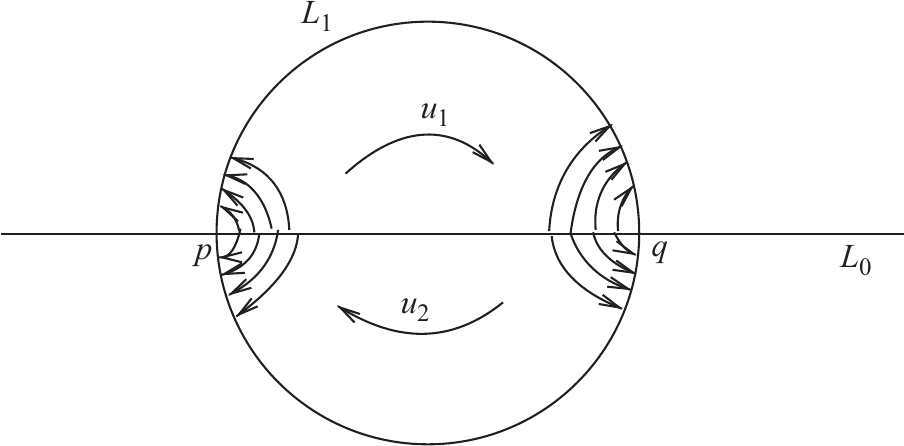
\includegraphics[width=.62\textwidth]{chapters/ch16-monotone-lagrangian-floer/figures/figure-16-1.png}
 \caption{全纯映射 $u_1,u_2$。}
 \label{fig:holomorphic-maps-u1-u2}
\end{figure}

由带边界的\personRiemann{}映射定理的简单应用可知，$\mathcal M(p,q;B_1)$ 恰有一个元素，
它由 $u_1:\mathbb R\times[0,1]\to\mathbb C$ 代表，其像为显然的上半圆盘（图
\ref{fig:holomorphic-maps-u1-u2}）。类似地，$\mathcal M(q,p;B_2)$ 恰有一个元素，
其像为下半圆盘。再对\personRiemann{}--\personHilbert{}问题作简单线性分析，还可证明这些映射正则，
即其线性化映射满射。由维数考察得到
\[
 \partial([\ell_p,w])=[q,w\#B_1],
 \qquad
 \partial([\ell_q,w'])=[p,w'\#B_2],
\]
其中 $w,w'$ 分别遍历 $\ell_p,\ell_q$ 的\termBoundingDisc{}。
\end{example}

\begin{exercise}
\label{ex:prove-plane-boundary-formula}
证明上述断言。
\end{exercise}

现在分析 $\mathcal M(p,p;B)$。把 $\mathcal M(p,p;B)$ 的每个元素视为对应于
$\widetilde{\mathcal M}(p,p;B)$ 中元素的无参数化曲线，由\personRiemann{}映射定理可证，
它由 $-1<\ell<1$ 时的全纯映射 $u_\ell:\mathbb R\times[0,1]\to\mathbb C$
组成，并满足
\[
 \begin{gathered}
 u_\ell(\mathbb R\times\{0\})\subset\mathbb R\times\{0\},\qquad
 u_\ell(\mathbb R\times\{1\})\subset\partial D^2,\qquad [u_\ell]=B,\\
 u_\ell(-\infty,\cdot)=u_\ell(\infty,\cdot)=\ell_p,\qquad
 u_\ell(0,0)=(\ell,0).
 \end{gathered}
\]
由对称性，$u_\ell$ 还必满足 $u_\ell(0,1)=(1,0)$。可以证明，上述族确实给出
$\mathcal M(p,p;B)$ 的全部元素，并且所有映射都是\personFredholm{}正则的。由此描述，
$\mathcal M(p,p;B)$ 的一个自然紧化是在 $\ell\to1$ 的一端添入断裂流线
$u_1\#u_2$，并添入 $\ell\to-1$ 时的另一端。

\begin{figure}[htbp]
 \centering
 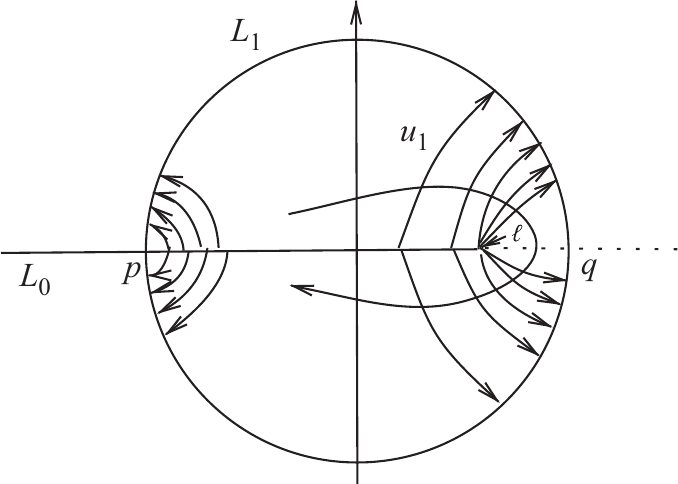
\includegraphics[width=.58\textwidth]{chapters/ch16-monotone-lagrangian-floer/figures/figure-16-2.png}
 \caption{全纯映射 $u_\ell$。}
 \label{fig:holomorphic-maps-ul}
\end{figure}

见图\ref{fig:holomorphic-maps-ul}。注意 $u_\ell$ 满足：
\begin{enumerate}[label=(\arabic*)]
\item $u_\ell(\mathbb R\times\{0\})\subset\{(t,0)\mid-1<t\leq\ell\}$；特别地，
当 $\ell\to-1$ 时，$u_\ell|_{\mathbb R\times\{0\}}$ 收敛到常值映射 $(-1,0)$；
\item $u_\ell|_{\mathbb R\times\{1\}}$ 的像恰好绕边界 $\partial D^2$ 一周。
\end{enumerate}
还可以验证，对任意紧子集
$K\subset\mathbb R\times[0,1]\setminus\{(0,1)\}$，
\[
 \|du_\ell\|_{\infty,K}\longrightarrow0\quad(\ell\to-1),
\]
同时还有
\[
 |du_\ell(0,1)|\nearrow\infty.
\]

由此分析可知，当 $\ell\to-1$ 时，上图背后的真实情形是出现了与如下奇异曲线
对应的\emph{稳定}流线：
\[
 (u_\infty,\mathbb R\times[0,1],\{(0,1)\})
 \cup(w,D^2,\{\mathrm{pt}\}).
\]
这里 $(u_\infty,\mathbb R\times[0,1],(0,1))$ 是主分支，
$u_\infty:\mathbb R\times[0,1]\to\mathbb C$ 是取常值
$p=(-1,0)$ 的映射，其定义域满足
\[
 (\mathbb R\times[0,1],\{(0,1)\})
 \cong(D^2\setminus\{\pm1\},\{\sqrt{-1}\}),
\]
而 $w:(D^2,\partial D^2)\to(\mathbb C,L_1)$ 是显然的包含映射，其定义域为边界
$\partial D^2$ 上带一个标记点的圆盘 $D^2$。

这个位形是一条可容许的稳定流线：$u_\infty$ 的定义域在边界上有三个特殊点，故它
稳定；$w$ 是非常值映射，故也稳定，因而两个映射的自同构群都平凡。对
$\mathcal M(p,p;B)$ 的上述分析计算出矩阵元
\[
 \bigl\langle(\partial\circ\partial)([\ell_p,w]),[\ell_p,w\#B]\bigr\rangle=1
\]
以及
\[
 \bigl\langle(\partial\circ\partial)([\ell_p,w]),[\ell_p,w\#B']\bigr\rangle=0
\]
（对任意 $B'\in\pi_2(p,p)$ 且 $B'\neq B$）。这清楚表明
$\partial\circ\partial\neq0$。

这个例子说明，当 $\mu(B)=2$ 时，$\mathcal M(p,p;B)$ 的边界可以含有并非断裂流线
类型的分支。还要注意，\emph{上述圆盘 $w$ 的马斯洛夫指标为 $2$}；稍后我们将看到，这并非
巧合。

事实上，对无边界紧\personRiemann{}曲面中的嵌入拉格朗日子流形而言，上述障碍是定义\personFloer{}同调的唯一障碍。在曲面上，每个一维子流形都是拉格朗日的，故紧嵌入拉格朗日子流形
是嵌入圆周的有限不交并。下面的曲面一般定理概括了这一讨论。

\begin{theorem}
\label{thm:surface-unobstructed-floer}
设 $\Sigma$ 是带面积形式的定向紧曲面。以 $\mathcal E_\Sigma^{\mathrm{ad}}$ 表示所有
连通分支都非零伦的嵌入拉格朗日子流形之集合。则对任意
$L_1,L_2\in\mathcal E_\Sigma^{\mathrm{ad}}$，取适当的\personNovikov{}环后，\personFloer{}同调
$HF(L_1,L_2;\Lambda)$ 有良定义。
\end{theorem}

在此意义下给出如下定义。

\stfhSubIndex{I189}{Wuzhangai}{无障碍（unobstructed）}{Qianruquxiandewuzhangaixing}{嵌入曲线的无障碍性（of embedded curves）}
\begin{definition}
\label{def:unobstructed-curve-surface}
设 $\Sigma$ 是带面积形式的定向紧曲面。若嵌入曲线 $\gamma\subset\Sigma$（不必连通）
没有零伦的连通分支，则称它是\termUnobstructed{}的。
\end{definition}

这是 (FOOO09) 所引入定义在二维曲面上的拉格朗日子流形情形之特例。关于高亏格曲面\termFukayaCategory{}的详细研究，可参见 (Ab08)；其中\personAbouzaid{}计算了 $\Sigma$ 上导出\personFukaya{}范畴的\personGrothendieck{}群。

\section{单调拉格朗日子流形的例子}
\label{sec:examples-monotone-lagrangians}

如二维例子所示，一般拉格朗日子流形对子 $(L_0,L_1)$ 的\personFloer{}同调会遇到障碍。
对这一障碍及其形变理论的完整研究需要超出本书层次的数学；(FOOO09) 已对此作了
彻底处理，有意了解细节的读者可参阅该书。

\personFloer{}在 (Fl89b) 中引入单调辛流形的概念，以克服其研究哈密顿\personFloer{}同调时遇到的
横截性困难。

\begin{remark}
\label{rem:general-perturbation-transversality}
在一般构造\personGromov{}--\personWitten{}不变量所涉及的模问题中，利用殆复结构以外的扰动研究
横截性的一般途径，最早由\personKontsevich{}在其著名论文 (Kon95) 中提出。

\stfhIndex{I117}{Cangxijiegou}{仓西结构（Kuranishi structure）}
\stfhIndex{I155}{Duozhongzhedietujing}{多重折叠途径（polyfold approach）}
如今，这种一般扰动横截性理论本质上有两种不同途径：一种是\emph{有限维壳上}途径，另一种
是\emph{无穷维离壳}途径。前一种是\personFukaya{}与\personOno{} (FOn99) 所采用的\termKuranishiStructure{}与多截面
方法，它是求解非线性方程的经典\personLyapunov{}约化方法之加强形式（相关构造亦见
(LT98)）；代数几何学家在 (LiT98)、(Be97)、(BF97) 中也采用这一途径。后一种途径
由\personBerndSiebert{} (Sie99) 采用，较近则以\personHofer{}、\personKrzysztofWysocki{}与\personZehnder{}的\termPolyfold{}途径
(HWZ07)、(H08) 为代表，尝试在离壳设置中对原方程作整体扰动（相关构造亦见
(Ru99)）。

即使 (FOn99) 问世二十年之后，这个横截性问题仍然是一个即便在辛几何专家之间也
需要进一步澄清的问题。
\end{remark}

受\personFloer{}对单调辛流形研究的启发，作者在 (Oh93a) 中挑出了单调拉格朗日子流形这一
类，以便把\personFloer{}对对子 $(L_0,L_1)$ 的同调理论构造推广到正合情形之外。这类拉格朗日
子流形避开了开\personRiemann{}曲面（亏格为零）的紧化模空间所涉及的大部分复杂横截性问题，
并使人能够无缝推广\personFloer{}的定义，依定义 16.1.1 中\personFloer{}原来的定义来定义映射
$\partial:CF(L_0,L_1)\to CF(L_0,L_1)$。

然而，(Oh93a) 已经注意到、(Oh95a) 后来又进一步强调，即使在这一良好情形中，也可能
出现\termAnomaly{}，即
\begin{equation}
 \partial^2\neq0,
\label{eq:monotone-boundary-anomaly}
\end{equation}
除非对子 $(L_0,L_1)$ 满足某个与马斯洛夫指标为 $2$ 的全纯圆盘之几何密切相关的
相容性条件。

\begin{remark}
\label{rem:role-of-monotonicity}
从内蕴辛拓扑的观点看，单调性既不自然也不灵活，因此它在一般辛拓扑中的作用对作者
而言尚未完全清楚。不过，它足以丰富地展示全纯圆盘如何在\personFloer{}同调中产生\emph{\termAnomaly{}}与
\emph{障碍}，并在\emph{非正合}背景下检验各种\personFloer{}理论构造。以某种方式处理上述障碍后，它也
自然推广了曲面上拉格朗日子流形\personFloer{}同调的讨论。在尝试借助障碍--形变理论与\termKuranishiStructure{}技术，把各种代数和几何结构完整实现于一般拉格朗日子流形的背景中
之前，单调情形是一个很好的试验场。近来，与（几乎）环面流形及镜像对称相关的许多
有趣单调拉格朗日环面例子已被发现；见 (FOOO12a)、(Wu12)、(Via13, Via14)。
\end{remark}

下面给出单个拉格朗日子流形版本的 $G(L_0,L_1;\ell_0)$；它也类似于环境辛流形
$(M,\omega)$ 的群
\[
 \Gamma_\omega=\Gamma(M,\omega)
 =\frac{\pi_2(M)}{\ker\omega\cap\ker c_1}.
\]
以 $I_\omega:\pi_2(M,L)\to\mathbb R$ 表示辛面积的取值。另定义整值同态
$I_\mu:\pi_2(M,L)\to\mathbb Z$：
\[
 I_\mu(\beta)=\mu\bigl(w^*TM,(\partial w)^*TL\bigr),
\]
其中右端是丛对
\[
 (w^*TM,(\partial w)^*TL)
\]
的马斯洛夫指标，而 $w:(D^2,\partial D^2)\to(M,L)$ 是 $\beta$ 的一个（因而
任意一个）代表。

\begin{definition}
\label{def:lagrangian-novikov-group}
定义
\[
 G(L;\omega)=\frac{\pi_2(M,L)}{\ker I_\omega\cap\ker I_\mu},
\]
并把 $\Lambda_{(L;\omega)}$ 定义为相应的\personNovikov{}环。
\end{definition}

简要回顾\personNovikov{}环 $\Lambda_{(\omega,L)}(R)$ 及其子环
$\Lambda_{0,(\omega,L)}(R)$ 的基本性质，其中 $R$ 是交换环，例如可取
$\mathbb Z_2$、$\mathbb Z$ 或 $\mathbb Q$。令
\[
 q^\beta=T^{\omega(\beta)}e^{\mu_L(\beta)},
\]
并令
\[
 \deg(q^\beta)=\mu_L(\beta),\qquad E(q^\beta)=\omega(\beta),
\]
于是 $\Lambda_{(\omega,L)}$ 与 $\Lambda_{0,(\omega,L)}$ 一般成为分次环。典范赋值
$\nu:\Lambda_{(\omega,L)}\to\mathbb R$ 定义为
\[
 \nu\left(\sum_\beta a_\beta T^{\omega(\beta)}e^{\mu_L(\beta)}\right)
 =\min\{\omega(\beta)\mid a_\beta\neq0\}.
\]
它诱导子环 $\Lambda_{0,(\omega,L)}\subset\Lambda_{(\omega,L)}$ 上的赋值，并进而
诱导其上的自然滤过。这使 $\Lambda_{(\omega,L)}$ 成为滤过分次环。对一般拉格朗日
子流形，该环甚至不必是\personNoether{}环。

下面定义单调拉格朗日子流形。

\stfhIndex{I131}{JixiaoMasiluofushu}{极小马斯洛夫数（minimal Maslov number）}
\stfhSubIndex{I133}{Dandiaolagelangriziliuxing}{单调拉格朗日子流形（monotone Lagrangian submanifold）}{Dingyi}{定义（definition）}
\begin{definition}
\label{def:monotone-lagrangian}
若紧拉格朗日子流形 $L\subset(M,\omega)$ 满足
\[
 I_\omega=\lambda I_\mu\qquad\text{对某个 }\lambda\geq0,
\]
则称 $L$ 是单调的。定义\emph{\termMinimalMaslovNumber{}} $\Sigma_L$ 为
$\operatorname{Im}I_\mu$ 的正生成元。
\end{definition}

\begin{exercise}
\label{ex:monotone-lagrangian-ambient}
证明单调拉格朗日子流形只存在于单调辛流形上。
\end{exercise}

\stfhIndex{I196}{Ruozhenghe}{弱正合（weakly exact）}
注意，所谓弱正合情形，即 $I_\omega=0$ 的情形，平凡地包含在上述情形中。若忽略
分次问题，则它可以完全按照正合情形 $\pi_2(M,L)=\{0\}$ 来研究。因此，本小节讨论
中假设 $L\subset M$ 单调、$\lambda>0$ 且 $I_\mu\neq0$。

下面的命题展示了这类拉格朗日子流形相对于一般拉格朗日子流形所具有的某些特殊辛
拓扑性质。

\begin{proposition}
\label{prop:monotone-lagrangian-group-rank-one}
设 $L\subset(M,\omega)$ 是单调拉格朗日子流形。则 $G(L;M,\omega)$ 是秩为 $1$
的自由\personAbel{}群，而 $\Lambda_{0,(\omega,L)}$ 成为一个离散赋值环，其剩余域是
$\Lambda_{(\omega,L)}$。
\footnote{译者注：原书此前把该群定义为 $G(L;\omega)$，本命题改写为
$G(L;M,\omega)$；且把 $\Lambda_{(\omega,L)}$ 称作
$\Lambda_{0,(\omega,L)}$ 的“剩余域”。译文照录，留待统一裁决。}
\end{proposition}

\stfhIndex{I056}{Kelifudehuanmian}{克利福德环面（Clifford torus）}
$\mathbb{RP}^n\subset\mathbb{CP}^n$ 以及例 5.19 中的\personClifford{}环面，都是单调
拉格朗日子流形的例子。

\begin{proposition}
\label{prop:clifford-torus-monotone}
考虑\personClifford{}环面 $T^n\subset\mathbb P^n$：
\[
 T^n=\{[z_0:z_1:\cdots:z_n]\in\mathbb P^n\mid |z_i|=1\}.
\]
该环面单调，其相伴群 $G(T^n;\mathbb P^n)$ 同构于 $\mathbb Z$。
\end{proposition}

\begin{proof}
容易验证
\[
 \pi_2(\mathbb P^n,T^n)\cong\pi_1(T^n)\oplus\pi_2(\mathbb P^n).
\]
若以 $\beta_i$ 表示圆盘
\[
 D_i=\{[z_0:z_1:\cdots:z_n]\in\mathbb P^n
 \mid z_j\equiv e^{\sqrt{-1}\theta_i^0}\text{ 对 }j\neq i\text{ 固定}\}
\]
之类，则在 $\pi_2(\mathbb P^n,T^n)$ 中有关系
\[
 \beta_0+\cdots+\beta_n=\alpha,
\]
其中 $\alpha$ 是 $\pi_2(\mathbb P^n)$ 的（正）生成元。又有
\begin{equation}
\begin{aligned}
 \mu(\beta_i)&=2=\frac{c_1(\alpha)}{n+1},\\
 \omega(\beta_i)&=\frac{\omega(\alpha)}{n+1}=2\pi.
 \end{aligned}
\label{eq:clifford-torus-monotonicity}
\end{equation}
\footnote{译者注：对 $\mathbb P^n$ 的标准正生成元通常有
$c_1(\alpha)=n+1$，故原书所印 $2=c_1(\alpha)/(n+1)$ 与此不相容；译文照录。}
这就证明了单调性。

此外，\eqref{eq:clifford-torus-monotonicity} 还蕴含所有 $\beta_i$ 在
$G(T^n;\mathbb P^n)$ 中定义同一个元素，记为 $\beta$，且
$\alpha=(n+1)\beta$。因此
\[
 G(T^n;\mathbb P^n)=\mathbb Z\cdot[\beta]\cong\mathbb Z.
\]
\end{proof}

再考虑其他标准环面
\[
 T_{(c_0,\ldots,c_n)}
 =\{[z_0:\cdots:z_n]\in\mathbb P^n\mid |z_i|=c_i>0\}.
\]
它们并不单调。以 $\beta_i$ 和 $\alpha$ 表示与上述
$c_0=\cdots=c_n$ 情形类似定义的类。依赖于数集
\[
 \{\omega(\beta_0),\ldots,\omega(\beta_n),\omega(\alpha)=2\pi\}
\]
的有理相关性，$G(T_{(c_0,\ldots,c_n)};\mathbb P^n)$ 的秩在 $1$ 与 $n+1$
之间变化。该例可进一步推广到环面流形的拉格朗日环面纤维；(CO06)、
(FOOO10b, FOOO11a) 对此作了细致分析。

单调性条件主要是为寻找一个条件而设计的，使 (Oh93a) 所定义的朴素\personFloer{}同调能够
构造。不过，第 3.7.2 节所述拉格朗日悬挂构造保持这一条件。

\begin{proposition}
\label{prop:monotone-suspension}
设 $L\subset(M,\omega)$ 是任意紧单调拉格朗日嵌入，$(h,\psi)$ 是第 3.7.2 节
意义下它的正合拉格朗日圈。则相伴悬挂
\[
 \iota_{(h,\psi)}:S^1\times L\longrightarrow T^*S^1\times M
\]
关于 $T^*S^1\times M$ 上的直和辛形式 $\omega_0\oplus w$ 是具有相同\termMonotonicityConstant{}的
单调拉格朗日嵌入。
\footnote{译者注：原书此处的直和辛形式印作 $\omega_0\oplus w$，而环境辛形式一直
记作 $\omega$；译文照录。}
\end{proposition}

\begin{exercise}
\label{ex:prove-monotone-suspension}
证明该命题。
\end{exercise}

还从命题 3.7.7 回忆，$\iota_{(h,\psi)}$ 在 $T^*S^1\times M$ 中哈密顿同痕于乘积
嵌入 $o_{S^1}\times L$。

\stfhIndex{I154}{Boerjieluoweiqi}{波尔捷罗维奇（Polterovich）}
\personPolterovich{}在研究 $\Ham(S^2)$ 的\personHofer{}直径时利用了上述命题，并把拉格朗日\personFloer{}同调的\personKunneth{}公式的一个版本应用于 $S^2$ 的赤道，巧妙地证明了下面的定理。第
17.6 节将依原论文 (Po98b) 给出证明。

\begin{theorem}[\personPolterovich{}]
\label{thm:hofer-diameter-s2-infinite}
$\Ham(S^2)$ 的\personHofer{}直径为无穷。
\end{theorem}

下面说明第 3.7.3 节所述\personChekanov{}环面 (Che96b) 的一个变体。

\begin{example}[在 $S^2\times S^2$ 中的\personChekanov{}环面]
\label{ex:chekanov-torus-s2xs2}
\personChekanov{}的环面最初通过把第 3.7.3 节所述悬挂构造用于标准圆周
$S^1\subset\mathbb C$ 而在 $\mathbb C^2$ 中构造（见例 16.3.6(3)）。适当选择\personChekanov{}悬挂中出现的参数，可将该环面嵌入 $S^2\times S^2$，成为一个奇异单调
拉格朗日环面：它与乘积
$S^1_{\mathrm{eq}}\times S^1_{\mathrm{eq}}\subset S^2\times S^2$ 不哈密顿同痕
（证明见 (EP10)、(FOOO12a)）。其构造可描述如下（此描述见 (AF08)）。把
$S^2\times S^2\setminus\overline\Delta$ 等同于单位圆盘丛 $D^1(TS^2)$。
(AF08) 中研究的拉格朗日环面，是 $\partial D^r(TS^2)$ 上经过一个给定点（比如北极
$N$）的简单闭定向测地线之并。适当选取 $r>0$，可以证明该环面在
$S^2\times S^2\supset D^1(TS^2)$ 中单调。把它记作 $T(r)$。
\end{example}

\begin{exercise}
\label{ex:unique-monotone-chekanov-radius}
证明上述例子中恰有一个 $0<r<1$ 的选择使环面 $T(r)$ 单调，并求出 $r$。
\end{exercise}

\personChekanov{}与\personSchlenk{} (CS10) 在辛向量空间或复射影空间中构造了许多单调拉格朗日环面，
并研究了其中哪些例子彼此不同。

\stfhIndex{I146}{Dandiankaigeluomofu-Weitengbubianliang}{单点开格罗莫夫--威腾不变量（one-point open Gromov--Witten invariant）}
\section{\termOnePointOpenGromovWittenInvariant{}}
\label{sec:one-point-open-gw-invariant}

单调拉格朗日子流形的一个良好性质，是不存在第 10.6 节所述的\emph{负多重覆叠问题}。
这是因为每个非常值伪全纯圆盘都具有正马斯洛夫指标。由此可以定义不依赖于相容殆复
结构选择的\emph{开\personGromov{}--\personWitten{}不变量}。

本节依照 (Oh95a) 的说明，构造这一\emph{单点不变量}并证明其辛不变性。

对相容殆复结构 $J_0$，定义
\[
 \widetilde{\mathcal M}(L;\beta;J_0)
 =\{w:(D^2,\partial D^2)\to(M,L)\mid
 \overline\partial_Jw=0,\ w(\partial D^2)\subset L,\ [w]=\beta\}
\]
及其商
\[
 \mathcal M(L;\beta;J_0)
 =\widetilde{\mathcal M}(L;\beta;J_0)/PSL(2,\mathbb R).
\]
回忆指标公式
\begin{equation}
 \operatorname{vir.dim}\widetilde{\mathcal M}(L;\beta;J_0)
 =n+\mu_L(\beta),
\label{eq:disc-moduli-virtual-dimension}
\end{equation}
其中 $\mu_L(\beta)$ 是丛对 $(w^*TM,(\partial w)^*L)$ 的马斯洛夫指标
$\mu(w^*TM,(\partial w)^*L)$，而 $w$ 是
$\widetilde{\mathcal M}(L;\beta;J_0)$ 的某个（因而任意一个）元素。
\footnote{译者注：原书两次把边界丛写作 $(\partial w)^*L$，而非通常的
$(\partial w)^*TL$；译文照录。}
我们还考察带一个标记点的 $J_0$-全纯圆盘模空间
$\mathcal M_1(L;\beta;J_0)$。

给定光滑道路 $J:[0,1]\to\mathcal J_\omega$，定义参数化模空间
\[
 \mathcal M^{\mathrm{para}}(L;\beta;J)
 =\coprod_{t\in[0,1]}\{t\}\times\mathcal M(L;\beta;J(t)),
\]
\[
 \mathcal M_1^{\mathrm{para}}(L;\beta;J)
 =\coprod_{t\in[0,1]}\{t\}\times\mathcal M_1(L;\beta;J(t)),
\]
把它们看作 $[0,1]$ 上的纤维化。下面给出紧性结果。

\begin{proposition}
\label{prop:minimal-maslov-two-disc-compactness}
设 $L\subset(M,\omega)$ 单调，其\termMinimalMaslovNumber{} $\Sigma_L\geq2$。
设 $\beta\in\pi_2(M,L)$ 满足 $\mu(\beta)=2$。则：
\begin{enumerate}[label=(\arabic*)]
\item 对任意相容殆复结构 $J_0$，$\mathcal M(L;\beta;J_0)$ 与
$\mathcal M_1(L;\beta;J_0)$ 都紧；
\item 对道路 $J:[0,1]\to\mathcal J_\omega$，参数化模空间
$\mathcal M^{\mathrm{para}}(L;\beta;J)$ 与
$\mathcal M_1^{\mathrm{para}}(L;\beta;J)$ 都紧。
\end{enumerate}
\end{proposition}

\begin{proof}
这是开情形稳定映射紧性定理的直接推论。这里只证明第一条。设
$w_i\in\widetilde{\mathcal M}(L;\beta;J_0)$ 是一个序列。需要证明 $w_i$ 有一个
子序列，在模去 $PSL(2,\mathbb R)$ 作用后收敛到稳定映射。

由于 $[w_i]=\beta$ 固定，
\[
 E_{J_0}(w_i)=\int w_i^*\omega=\omega(\beta),
\]
故序列 $w_i$ 具有一致能量上界。稳定映射紧性定理于是说明，可以选取一个仍记作
$w_i$ 的子序列，收敛到稳定映射
\[
 w_\infty=\sum_{\ell=1}^{N}v_\ell,
\]
其中每个 $v_\ell$ 或为 $J_0$-全纯圆盘，或为 $J_0$-全纯球面。若 $v_\ell$ 是球面，
以 $\mu(v_\ell)$ 表示 $2c_1(v_\ell)$；若它是边界落在 $L$ 上的圆盘，则以
$\mu(v_\ell)$ 表示其马斯洛夫指标。

由于 $\mu(\beta)=2$ 极小，且
\[
 2=\mu(w_\infty)=\sum_{\ell=1}^{N}\mu(v_\ell),
\]
单调性蕴含上述和中至多有一个非常值分支。另一方面，$w_\infty$ 的稳定性又蕴含其中
不能有常值分支。因此必有 $N=1$，从而 $w_i$ 经适当重参数化后确实收敛。

类似论证证明 $\mathcal M_1(L;\beta;J_0)$ 及参数化空间的紧性。
\end{proof}

下面回忆通过扰动殆复结构得到的横截性结果。设 $L\subset(M,\omega)$ 是任意紧单调
拉格朗日子流形，以
\[
 \widetilde{\mathcal M}^{\mathrm{inj}}(L;\beta;J_0)
 \subset\widetilde{\mathcal M}(L;\beta;J_0)
\]
表示由\termSomewhereInjective{}的 $J_0$-全纯圆盘组成的子集。

闭曲面情形的如下基本横截性结果已在第 10.4、10.5 节证明。

\begin{proposition}
\label{prop:disc-evaluation-transversality}
设 $x\in L$。存在稠密子集
$\mathcal J_\omega(L,x)\subset\mathcal J_\omega$，使对所有
$\beta\in\pi_2(M,L)$：
\begin{enumerate}[label=(\arabic*)]
\item $\widetilde{\mathcal M}^{\mathrm{inj}}(L;\beta;J_0)$ 横截；
\item $\operatorname{ev}_\beta:\mathcal M_1^{\mathrm{inj}}(L,\beta;J_0)\to L$
横截于 $x$。
\end{enumerate}
对 $J=\{J(t)\}_{0\leq t\leq1}$ 的参数化模空间，同样结论成立。
\end{proposition}

称这样的对子 $(J_0,x_0)$ 为\termTransversePair{}。对\termTransversePair{} $(J_0,x_0)$，命题
\ref{prop:minimal-maslov-two-disc-compactness} 与
\ref{prop:disc-evaluation-transversality} 蕴含：对任意满足 $\mu(\beta)=2$ 的
$\beta$，$\operatorname{ev}_\beta^{-1}(x_0)$ 是紧零维流形（若非空）。

\begin{lemma}
\label{lem:minimal-maslov-discs-somewhere-injective}
设 $J_0$ 是任意相容殆复结构，不必正则。设 $L\subset(M,\omega)$ 单调且
$\Sigma_L>0$，并取满足 $\mu(\beta)=\Sigma_L$ 的
$\beta\in\pi_2(M,L)$。则
\[
 \widetilde{\mathcal M}^{\mathrm{inj}}(L;\beta;J_0)
 =\widetilde{\mathcal M}(L;\beta;J_0),
\]
即对任意 $J_0\in\mathcal J_\omega$，
$\widetilde{\mathcal M}(L;\beta;J_0)$ 中所有 $J_0$-全纯圆盘都\termSomewhereInjective{}。特别地，命题\ref{prop:disc-evaluation-transversality} 对完整
模空间成立。
\end{lemma}

\begin{proof}
第一条来自\termMinimalMaslovNumber{} $\Sigma_L$ 的定义：由像的结构定理——球面情形的
定理 8.7.3，以及圆盘情形的 (Laz00)、(KO00)——无论 $J_0$ 正则与否，每个
$J_0$-全纯圆盘都必为单圆盘。第二条则由单调性假设与 $\mu(\beta)=\Sigma_L$ 立即
推出，因为它们排除了冒泡。
\end{proof}

记
\[
 \Phi_{J_0}(L;x_0)
 =\sum_{\beta:\,\mu(\beta)=2}\#\bigl(\operatorname{ev}_\beta^{-1}(x_0)\bigr).
\]
\emph{从此以后不再特别说明：对一般 $L$，计数取 $\mathbb Z_2$-系数；当拉格朗日子流形
$L$（相对）spin 时，使用 $\mathbb Z$-系数。}

\begin{lemma}
\label{lem:one-point-count-invariance}
设 $L\subset(M,\omega)$ 单调且 $\Sigma_L\geq2$。设 $(J_0,x_0)$ 与
$(J_1,x_1)$ 是\termTransversePair{}，并且 $[x_0]=[x_1]\in\pi_0(L)$。则
\[
 \Phi_{J_0}(L;x_0)=\Phi_{J_1}(L;x_1).
\]
\end{lemma}

\begin{proof}
固定嵌入道路 $\gamma:[0,1]\to L$，其中 $\gamma(0)=x_0$、$\gamma(1)=x_1$。
由评价横截性的参数化版本及横截性延拓定理，可选道路
$J:[0,1]\to\mathcal J_\omega$，使得对所有 $\mu(\beta)=2$ 的 $\beta$，
$\widetilde{\mathcal M}^{\mathrm{para}}(L;\beta;J)$ 横截，且评价映射
\[
 \begin{aligned}
 \operatorname{Ev}_\beta:
 \mathcal M_1^{\mathrm{para}}(L;\beta;J)&\longrightarrow[0,1]\times L,\\
 (t,(w,z))&\longmapsto(t,w(z))
 \end{aligned}
\]
横截于 $\Lambda=\operatorname{id}\times\gamma:[0,1]\to[0,1]\times L$。指标公式给出
\[
 \dim\mathcal M_1^{\mathrm{para}}(L;\beta;J)=n+1,
\]
故 $\operatorname{Ev}_\beta^{-1}(\Lambda)$ 是紧一维流形，其边界为
\[
 \{0\}\times\operatorname{ev}_\beta^{-1}(x_0)
 \coprod
 \{1\}\times\operatorname{ev}_\beta^{-1}(x_1).
\]
由紧一维流形的分类定理，
\[
 \#\bigl(\operatorname{ev}_\beta^{-1}(x_0)\bigr)
 =\#\bigl(\operatorname{ev}_\beta^{-1}(x_1)\bigr).
\]
依定义即得结论。
\end{proof}

由此可以如下定义单点 GW 不变量。

\begin{definition}
\label{def:one-point-open-gw-invariant}
设 $L\subset(M,\omega)$ 是紧单调拉格朗日子流形，$\Sigma_L\geq2$；以
$\pi\in\pi_0(L)$ 表示 $L$ 的一个连通分支。相对于 $\pi$ 的单点 GW 不变量定义为
\[
 \Phi(L;\pi)=\Phi_{J_0}(L;x_0),
\]
其中 $(J_0,x_0)$ 是满足 $[x_0]=\pi\in\pi_0(L)$ 的\termTransversePair{}。当 $L$ 连通时，简记
\[
 \Phi(L;\{\mathrm{pt}\})=\Phi_{J_0}(L;x_0),
\]
称其为 $L\subset(M,\omega)$ 的单点 GW 不变量。
\end{definition}

下面考察几个例子。

\begin{example}
\label{ex:one-point-open-gw-examples}
\begin{enumerate}[label=(\arabic*)]
\item \stfhPropertyLabel{（标准环面）} 考虑标准环面
\[
 T^n=\underbrace{S^1(1)\times\cdots\times S^1(1)}_{n\text{ 个}}
 \subset\mathbb C^n\cong\mathbb R^{2n}.
\]
有 $\pi_2(\mathbb C^n,T^n)\cong\pi_1(T^n)\cong\mathbb Z^n$。以
$\beta_i$（$i=1,\ldots,n$）表示由映射
\[
 \begin{aligned}
 w_i:(D^2,\partial D^2)&\longrightarrow(\mathbb C^n,T^n),\\
 w_i(z)&=(1,\ldots,\underbrace{z}_{i\text{th}},\ldots,1)
 \end{aligned}
\]
代表的 $\pi_2(\mathbb C^n,T^n)$ 的显然生成元。计算其马斯洛夫指标与辛面积可知，
该环面单调，\termMonotonicityConstant{}为 $\lambda=\pi$。这些映射显然是经过点
$x_0=(1,\ldots,1)$ 的全纯映射，故至少有 $n$ 个彼此不同、马斯洛夫指标为 $2$
的全纯圆盘。

\item \stfhPropertyLabel{（\personClifford{}环面）} 这次考虑\personClifford{}环面
$T^n\subset\mathbb{CP}^n$。它由 $\mathbb C^{n+1}$ 上乘积圆周作用的商
$T^{n+1}/S^1\subset S^{2n+1}/S^1\cong\mathbb{CP}^n$ 定义。在射影坐标中有全纯
圆盘
\[
 w_j:(D^2,\partial D^2)\to(\mathbb{CP}^n,T^n),
 \qquad z\longmapsto[1;\ldots;\underbrace{z}_{j\text{th}};\ldots;1]
\]
（$j=1,\ldots,n+1$）。把
$\Phi(T^n,\mathbb{CP}^n;\{\mathrm{pt}\})=n+1$ 的证明留作习题。

\item \stfhPropertyLabel{（\personChekanov{}环面）} 对标准圆周
$S^1(1)\subset\mathbb R^2\cong\mathbb C$ 施行\personChekanov{}悬挂，得到\personChekanov{}环面
\[
 \Theta_0(S^1(1))\subset\mathbb R^2,
 \qquad
 \Theta_0(S^1(1))=I_1(N_0\times S^1(1)).
\]
\footnote{译者注：原书把所得\personChekanov{}环面的环境写作 $\mathbb R^2$；但紧接着定义的
辛嵌入以 $T^*\mathbb R^2$ 为靶，维数提示这里可能有环境维数的排印问题。译文照录。}
这里 $N_0$ 是 $T^*S^1$ 的零截面，$I_1=(i_1^*)^{-1}$ 是辛嵌入
\[
 I_1=(i_1^*)^{-1}:T^*(\mathbb R\times S^1)\longrightarrow T^*\mathbb R^2,
\]
其中 $i_1:S^1\times\mathbb R\to\mathbb R^2$ 定义为
\[
 i_1(\theta,q)=(e^q\cos(2\pi\theta),e^q\sin(2\pi\theta)).
\]
\personEliashberg{}与\personPolterovich{}在 (EP97) 中证明
\[
 \Phi(\Theta_0(S^1(1));\{\mathrm{pt}\})=1.
\]
不久前，\personChekanov{}与\personSchlenk{}尝试对若干显式辛流形类上的单调拉格朗日子流形集合
作完整分类 (CS10)。
\end{enumerate}
\end{example}

\begin{exercise}
\label{ex:classify-minimal-maslov-discs-tori}
证明例\ref{ex:one-point-open-gw-examples} 中给出的 $\mathbb C^n$ 内标准环面及
$\mathbb{CP}^n$ 内\personClifford{}环面的圆盘全都横截，并且它们给出了经过环面中给定点
$x_0$ 的所有马斯洛夫指标为 $2$ 的全纯圆盘。（若计入这些圆盘的定向，则它们全都
正贡献，故
$\Phi(T^n,\mathbb C^n;\mathrm{pt})=n$ 且
$\Phi(T^n,\mathbb{CP}^n;\{\mathrm{pt}\})=n+1$。定向研究见第 15.4 节。）
\end{exercise}

\stfhIndex{I054}{Qiekanuofu}{切卡诺夫（Chekanov）}
上述单点不变量计算立即导出\personChekanov{}定理 (Che96b)。

\begin{theorem}[\personChekanov{}]
\label{thm:standard-chekanov-tori-not-symplectically-equivalent}
标准环面 $T^2=S^1(1)\times S^1(1)$ 与\personChekanov{}环面
$\Theta_0(S^1(1))$ 不辛等价。
\end{theorem}

\personChekanov{}最初通过考察\personEkeland{}--\personHofer{}容量序列的行为证明该定理。应指出，标准环面与\personChekanov{}环面都满足下列条件：
\begin{enumerate}[label=(\arabic*)]
\item \termMinimalMaslovNumber{}为 $2$；
\item \termMonotonicityConstant{}为 $\pi$；
\item 第一\personEkeland{}--\personHofer{}容量为 $2\pi$。
\end{enumerate}
因此，没有简单的经典方法区分标准环面与\personChekanov{}环面。

\section{\personFloer{}边界算子的\termAnomaly{}}
\label{sec:anomaly-floer-boundary-operator}

本节考察单调拉格朗日子流形对子 $(L_0,L_1)$ 的\personFloer{}边界之构造。特别地，我们分析
(13.9.28) 中低虚维数——即\personMaslov{}--\personViterbo{}指标为 $0,1,2$——的\personFloer{}模空间结构。
记
\[
 \widetilde{\mathcal M}([\ell_p,w],[\ell_q,w'])
\]
为光滑\personFloer{}流线的集合，即并集
\[
 \widetilde{\mathcal M}([\ell_p,w],[\ell_q,w'])
 :=\bigcup_{w\#B\simeq w'}\widetilde{\mathcal M}(p,q;B),
\]
其中 $\widetilde{\mathcal M}(p,q;B)$ 是先前定义的连接 $p,q\in L_0\cap L_1$、满足
$[u]=B\in\pi_2(p,q)$ 的光滑\personFloer{}流线集合。

\subsection{\personFloer{} \termPreBoundaryMap{}的定义}
\label{subsec:floer-pre-boundary-definition}

先注意，若\termMonotonicityConstant{}为正，且 $\beta$ 容许一个非常值伪全纯圆盘，则
$\mu(\beta)>0$。从如下引理开始。

\begin{lemma}
\label{lem:maslov-one-discs-avoid-finite-set}
设 $L$ 紧，$F\subset L$ 是任意有限子集。则存在
$\mathcal J_\omega$ 的稠密子集 $\mathcal J_L(F)$，使对任意
$J_0\in\mathcal J_L(F)$ 以及任意满足 $\mu(\beta)=1$ 的
$\beta\in\pi_2(L)$，评价链
\[
 \operatorname{ev}_\beta:\mathcal M_1(L,J_0;\beta)\longrightarrow L
\]
都不与 $F$ 相交。
\end{lemma}

\begin{proof}
由指标公式，
\[
 \dim\mathcal M_1(L,J_0;\beta)=n+\mu(\beta)+1-3=n-1<n.
\]
$F$ 是有限点集，特别是零维的。于是，基于评价横截性边界版本（定理 16.3.2）的
维数计算说明：通有地选择 $J_0$ 时，评价链
$\operatorname{ev}_\beta:\mathcal M_1(L,J_0;\beta)\to L$ 不与 $F$ 相交。以
$\mathcal J_L(F)$ 表示所有这种 $J_0$ 组成的子集。
\end{proof}

现在证明下述定理。

\begin{theorem}
\label{thm:low-index-monotone-floer-moduli}
设 $L_0,L_1$ 单调且\termMinimalMaslovNumber{}非零，并且
$J_i\in\mathcal J_{L_i}(L_0\cap L_1)$（$i=0,1$），其中
$\mathcal J_{L_i}(L_0\cap L_1)$ 如引理
\ref{lem:maslov-one-discs-avoid-finite-set}。则存在子集
$\mathfrak j^{\mathrm{reg}}_{(L_0,L_1)}(J_0,J_1)\subset\mathfrak j_\omega$，
使对任意 $J\in\mathfrak j^{\mathrm{reg}}_{(L_0,L_1)}(J_0,J_1)$，下列断言成立：
\begin{enumerate}[label=(\arabic*)]
\item 对所有 $p,q\in L_0\cap L_1$ 和满足 $\mu(p,q;B)<0$ 的
$B\in\pi_2(p,q)$，$\mathcal M(p,q;B;J)=\varnothing$；
\item 对所有 $p,q\in L_0\cap L_1$ 和满足 $\mu(p,q;B)=0$ 的
$B\in\pi_2(p,q)$，除非 $p=q$ 且 $B=0\in\pi_2(p,q)$，否则
$\mathcal M(p,q;B;J)=\varnothing$；
\item 对所有 $p,q\in L_0\cap L_1$ 和满足 $\mu(p,q;B)=1$ 的
$B\in\pi_2(p,q)$，$\mathcal M(p,q;B;J)$ 是紧的零维流形，因而为有限集。
\end{enumerate}
\end{theorem}

\begin{proof}
证明基于指标公式 (16.3.3)、命题 15.1.5 与 16.3.2 的维数计算及相交论证。

由引理 15.1.4，$\mathbb R$ 自由作用于任意非常值流线 $u$（证明见 (Oh97a)）。
特别地，对任意\personFredholm{}正则 $J$，只要
$\widetilde{\mathcal M}(p,q;B;J)\neq\varnothing$，并且 $p\neq q$，或 $p=q$ 但
$B\neq0$，就有
\[
 \dim\widetilde{\mathcal M}(p,q;B;J)\geq1.
\]
（当 $p=q$ 时，可把 $\pi_2(p,p)$ 的每个元素等同于 $\pi_2(L_0)$ 或
$\pi_2(L_1)$ 中的元素。）因此，对
$J\in\mathfrak j^{\mathrm{reg}}_{(L_0,L_1)}(J_0,J_1)$，(1)、(2) 立即成立。
\footnote{译者注：原书证明此处把上述正则集合印作
$\mathcal P^{\mathrm{reg}}_{(L_0,L_1)}(J_0,J_1)$，与定理陈述中的
$\mathfrak j^{\mathrm{reg}}_{(L_0,L_1)}(J_0,J_1)$ 不一致；译文依定理记号补正。}

当 $\mu(p,q;B)=1$ 时，对任意 $(L_0,L_1)$-正则 $J$，
$\mathcal M(p,q;B;J)$ 都是零维的。只需证明它紧。否则存在序列
$u_i\in\mathcal M(p,q;B;J)$，当 $i\to\infty$ 时发生分裂或冒泡。

若 $u_i$ 在极限处分裂为 $(u_{\infty,1},u_{\infty,2})$，其中
$u_{\infty,1}\in\mathcal M(p,r;B_1)$、
$u_{\infty,2}\in\mathcal M(r,q;B_2)$，则
\[
 1=\mu(p,r;B_1)+\mu(r,q;B_2).
\]
因此二者的指标分别为 $1,0$，次序任意。但 $\mu(r,q;B_2)=0$ 意味着
$\dim\widetilde{\mathcal M}(r,q;B_2)=0$，除非 $r=q$ 且 $B_2=0$，否则不可能。
此时 $u$ 必须是常值条带，而这又不可能：这种圆盘具有由 $\tau$-平移产生的连续
$\mathbb R$-自同构群，故在模空间的稳定映射紧化定义中，其定义域会被压缩。注意
$\mathbb R\times[0,1]$ 共形等价于带两个标记点的圆盘，而后者不是稳定曲线。因此
$\mathcal M(p,q;B;J)$ 不可能有分裂端。

若 $u_i$ 发生冒泡，单调性蕴含每个气泡都有正指标。因此，球面气泡的指标至少为
$2>1$，维数计算排除了这种冒泡。唯一剩余可能是形如 $(u_0,w)$ 的极限，其中
$u_0\in\mathcal M(p,q;B';J)$，$w$ 是 $(L_0,J_0)$ 或 $(L_1,J_1)$ 的非常值圆盘
气泡。此时
\[
 1=\mu(p,q;B')+\mu(w).
\]
单调性再次给出 $\mu(w)>0$，故必有 $\mu(w)=1$、$\mu(p,q;B')=0$。后一等式蕴含
$p=q$、$B'=0$，所以 $u_0$ 是常值流线 $u_0\equiv p$。\personGromov{}--\personFloer{}极限之像的
连通性于是蕴含 $w$ 经过 $p\in L_0\cap L_1$。然而，由
$J_i\in\mathcal J_{L_i}(L_0\cap L_1)$ 的选择，引理
\ref{lem:maslov-one-discs-avoid-finite-set} 也排除了这种情形。
\end{proof}

除紧性外，另一个重要问题是模空间
$\mathcal M([\ell_p,w],[\ell_q,w'];J)$ 上的相容定向。第 15.6 节（亦见
(FOOO09)）已证明：若对子 $(L_0,L_1)$ 相对 spin 并给定相对 spin 结构，则存在一种
典范方式在模空间族 $\mathcal M([\ell_p,w],[\ell_q,w'];J)$ 上赋予相容定向。因此，
当 $(L_0,L_1)$ 相对 spin 时，整数
\[
 n([\ell_p,w],[\ell_q,w'];J)
 =\#\mathcal M([\ell_p,w],[\ell_q,w'];J),
 \qquad
 \mu[\ell_q,w']=\mu([\ell_p,w])+1,
\]
\stfhIndex{I088}{Fuluoeryubianjieyingshe}{弗洛尔预边界映射（Floer pre-boundary map）}
有良定义。以它作为标准\personFloer{} \termPreBoundaryMap{}
\[
 \partial:CF_R^k(L_1,L_0;\ell_0)\longrightarrow CF_R^{k+1}(L_1,L_0;\ell_0)
\]
的矩阵元，定义
\[
 \partial([\ell_p,w])
 =\sum_{\mu(\ell_q,w')=\mu(\ell_p,w)+1}
 n([\ell_p,w],[\ell_q,w'])\cdot[\ell_q,w'].
\]
这里，当 $(L_0,L_1)$ 相对 spin 时 $R=\mathbb Z$，一般取 $R=\mathbb Z_2$。\personGromov{}--\personFloer{}紧性蕴含右端定义了 $CF_R^*(L_1,L_0;\ell_0)$ 中的元素，即满足\personNovikov{}有限性条件。因为\personFloer{}所定义的这个映射 $\partial$ 未必满足
$\partial^2=0$，所以称 $\partial$ 为\personFloer{} \termPreBoundaryMap{}。

\begin{figure}[htbp]
 \centering
 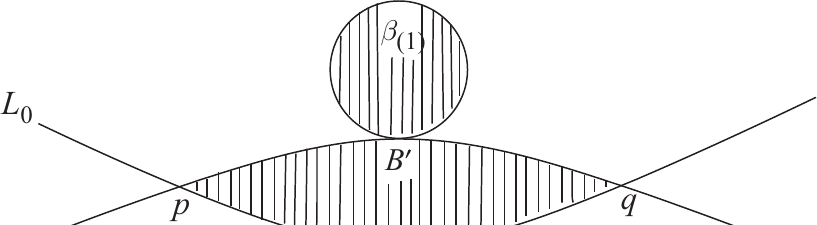
\includegraphics[width=.68\textwidth]{chapters/ch16-monotone-lagrangian-floer/figures/figure-16-3.png}
 \caption{余维 $1$ 的层 $\mathcal N(p,q;B';L_1,\beta_{(1)};J)$。}
 \label{fig:codimension-one-disc-bubble-stratum}
\end{figure}

\subsection{\termAnomaly{}与障碍}
\label{subsec:anomaly-and-obstruction}

现在研究\personFloer{} \termPreBoundaryMap{} $\partial$ 的边界性质。为此，需要分析虚维数为
$1$ 的模空间 $\mathcal M(p,q;B)$，并对每个这样的 $B$ 描述紧化模空间
$\overline{\mathcal M}(p,q;B)$ 中“余维 $1$”的奇异层。

考虑\personFloer{}流线模空间 $\widetilde{\mathcal M}(p,q;B';J)$ 及评价映射
\[
 \begin{aligned}
 \operatorname{ev}^{L_0}:\widetilde{\mathcal M}(p,q;B';J)&\to L_0,
 &(u,\tau)&\mapsto u(\tau,0),\\
 \operatorname{ev}^{L_1}:\widetilde{\mathcal M}(p,q;B';J)&\to L_1,
 &(u,\tau)&\mapsto u(\tau,1).
 \end{aligned}
\]
再考虑 $\mathcal M_1(L_0;\beta_{(0)};J_0)$、
$\mathcal M_1(L_1;\beta_{(1)};J_1)$ 及评价映射
\[
 \operatorname{ev}_0:\mathcal M_1(L_0;\beta_{(0)};J_0)\to L_0,
 \qquad
 \operatorname{ev}_1:\mathcal M_1(L_1;\beta_{(1)};J_1)\to L_1.
\]
下列集合描述 $\overline{\mathcal M}(p,q;B;J)$ 的余维 $1$ 层。

\begin{definition}
\label{def:disc-bubble-boundary-strata}
设 $p,q\in L_0\cap L_1$、$B'\in\pi_2(p,q)$，并且
$\beta_{(0)}\in G(L_0;\omega)$、$\beta_{(1)}\in G(L_1;\omega)$。对
$i=0,1$，令
\[
 \mathring{\mathcal N}(p,q;B':L_0,\beta_{(0)};J)
 =\widetilde{\mathcal M}(p,q;B';J)_{\operatorname{ev}^{L_0}}
 \!\times_{\operatorname{ev}_0}\mathcal M_1(L_0;\beta_{(0)};J_0)/\mathbb R,
\]
\[
 \mathring{\mathcal N}(p,q;B':L_1,\beta_{(1)};J)
 =\widetilde{\mathcal M}(p,q;B';J)_{\operatorname{ev}^{L_1}}
 \!\times_{\operatorname{ev}_1}\mathcal M_1(L_1;\beta_{(1)};J_1)/\mathbb R.
\]
见图\ref{fig:codimension-one-disc-bubble-stratum}。定义模空间
$\mathcal N(p,q;B':L_1,\beta_{(1)};J)$ 为
$\mathring{\mathcal N}(p,q;B':L_1,\beta_{(1)})$ 在
$\overline{\mathcal M}(p,q;B;J)$ 中的闭包，其中 $B=B'\#\beta_{(1)}$。
$\mathcal N(p,q;B':L_0,\beta_{(0)};J)$ 的定义类似，故略去。
\end{definition}

再定义
\begin{equation}
 \mathcal N([\ell_p,w],[\ell_q,w']:L_1;J)
 :=\bigcup_{\substack{(B',\beta_{(1)});\\
 [\ell_p,w]\#(B'\#\beta_{(1)})=[\ell_q,w']}}
 \mathcal N(p,q;B':L_1,\beta_{(1)};J),
\label{eq:total-disc-bubble-stratum}
\end{equation}
并类似定义 $\mathcal N([\ell_p,w],[\ell_q,w']:L_0;J)$。

我们希望说，当 $B=B'\#\beta_{(i)}$ 时，
$\mathcal N(p,q,B':L_i,\beta_{(i)};J)$ 在 $\mathcal M(p,q;B;J)$ 中具有“余维
$1$”。对一般拉格朗日对子 $(L_0,L_1)$，即便通有地选择 $J=\{J_t\}$，这句话也没有
意义。不过，若 $(L_0,L_1)$ 单调（更一般地，若它们半正且
$\mu_L(\beta_{(i)})\neq0$），则对通有选择的 $J$，情况确实如此。

\begin{theorem}
\label{thm:boundary-of-index-two-floer-moduli}
设 $L_0,L_1$ 单调，$J_0,J_1\in\mathcal J_\omega^0(L_0,L_1)$，并且
$J\in\mathfrak j^{\mathrm{reg}}_{(L_0,L_1)}(J_0,J_1)$ 如上。设
$p,q\in L_0\cap L_1$、$B\in\pi_2(p,q)$ 满足
\begin{equation}
 \mu(p,q;B)=2.
\label{eq:index-two-class}
\end{equation}
则：
\begin{enumerate}[label=(\arabic*)]
\item $\mathcal N(p,q;B':L_i,\beta_{(i)};J)$ 或者为空，或者是如下类型的紧零维
流形：
\[
 p=q,\qquad B'=0,\qquad\mu(\beta_{(i)})=2,
\]
它由位形 $u\#w$ 组成，其中 $u\equiv p$，而 $w$ 是经过 $p$ 的
$J_i$-全纯圆盘；
\item $\mathcal M(p,q;B;J)$ 是光滑一维流形，其边界是下列并：
\begin{equation}
\begin{aligned}
&\bigcup_{\substack{r\in L_0\cap L_1;\\B_1\#B_2=B}}
 \mathcal M(p,r;B_1;J)\#\mathcal M(r,q;B_2;J)\\
&\quad\cup
 \bigcup_{\substack{(B',\beta_{(1)});\\
 [\ell_p,w]\#(B'\#\beta_{(0)})=[\ell_q,w']}}
 \mathcal N(p,q;B':L_0,\beta_{(0)};J)\\
&\quad\cup
 \bigcup_{\substack{(B',\beta_{(1)});\\
 [\ell_p,w]\#(B'\#\beta_{(1)})=[\ell_q,w']}}
 \mathcal N(p,q;B:L_1,\beta_{(1)};J),
\end{aligned}
\label{eq:index-two-moduli-boundary}
\end{equation}
其中 $\mu(p,r;B_1)=\mu(r,q;B_2)=1$，且
$\mu(\beta_{(i)})=2$（$i=0,1$）。
\footnote{译者注：原书式 (16.4.6) 的第二个并（$L_0$ 项）仍以
$(B',\beta_{(1)})$ 为求并指标，而第三个并的被并对象写作
$\mathcal N(p,q;B:L_1,\beta_{(1)};J)$，不是与条件相应的 $B'$。译文逐项照录。}
\end{enumerate}
\end{theorem}

\begin{proof}
结论仍由基于模空间及评价映射横截性的维数计算得到。

先证 (1)。只考虑 $i=1$；$i=0$ 相同。依定义，
$\mathcal N(p,q;B':L_1,\beta_{(1)};J)$ 是纤维积
\[
 \frac{\widetilde{\mathcal M}(p,q;B';J)_{\operatorname{ev}^{L_1}}
 \times_{\operatorname{ev}_1}\mathcal M_1(L_1;\beta_{(1)};J_1)}{\mathbb R}
 =\frac{(\operatorname{ev}^{L_1}\times\operatorname{ev}_1)^{-1}(\Delta)}
 {\mathbb R},
\]
其中 $\Delta\subset L_1\times L_1$ 是对角线。回忆
\[
 \operatorname{vir.dim}\mathcal M_{(0;0,1)}(p,q;B')=\mu(p,q;B')-1,
\]
\[
 \operatorname{vir.dim}\mathcal M_1(L_1,J_1;\beta_{(1)})
 =n+\mu(\beta_{(1)})-2,
\]
且
\[
 \mu(p,q;B)=\mu(p,q;B')+\mu(\beta_{(1)}).
\]
由 $\mu(B)=2$，
\[
 \mu(p,q;B')=2-\mu(\beta_{(1)}),
\]
而 $\widetilde{\mathcal M}(p,q;B';J)$ 的横截性给出
$\mu(p,q;B')\geq0$。

若 $\Sigma_{L_1}\geq3$，这立即导致矛盾，故
$\mathcal N(p,q;B':L_1,\beta_{(1)})=\varnothing$。$i=0$ 亦同。因此，若
$\Sigma_{L_i}\geq3$，则 $\mathcal M(p,q;B;J)$ 是紧一维流形，边界只有分裂流线
类型。

现在考虑 $\Sigma_{L_1}=2$。此时可能有
$\mu(p,q;B')=0$、$\mu(\beta_{(1)})=2$。再次由
$\widetilde{\mathcal M}(p,q;B';J)$ 的横截性，这只有在
\[
 p=q,\qquad B'=0
\]
时发生。

\begin{remark}
\label{rem:constant-strip-with-disc-bubble-stable}
此时相伴映射 $u$ 是常值映射 $u\equiv p$。要强调的是，节点曲线
\[
 u\#w,\qquad [u]=0,\quad[w]=\beta_{(1)}
\]
是稳定映射。这是因为分支 $u\equiv p:\mathbb R\times[0,1]\to M$ 带有一个额外
特殊点 $z_0=(\tau_0,1)\in\mathbb R\times\{1\}$，气泡分支 $w$ 在此黏附。由于
$\mathbb R\times[0,1]\setminus\{z_0\}$ 共形同构于
$D^2\setminus\{1,-1,\sqrt{-1}\}$，常值分支 $u$ 定义稳定映射，故该位形是紧化\personFloer{}模空间 $\overline{\mathcal M}(p,q;B)$（其中
$B=B'\#\beta_{(1)}$）中容许的节点曲线。

\emph{应指出，到目前为止，上述论证没有使用圆盘模空间
$\mathcal M(L_i;\beta_{(i)})$ 的任何横截性断言，只使用了\personFloer{}流线模空间的
横截性}。
\end{remark}

由 $\Sigma_{L_1}=2$，$\mathcal M(L_1;\beta_{(1)};J_1)$ 的每个元素必\termSomewhereInjective{}。事实上，若
$v\in\mathcal M(L_1;\beta_{(1)};J_1)$ 不\termSomewhereInjective{}，则
[KOh00]、[Laz00] 中伪全纯圆盘的像结构定理蕴含存在
$v_i$（$i=1,\ldots,a$，$a\geq2$），使
$\sum_{i=1}^a[v_i]=[v]$，且 $\mathcal M(L_1;[v_i];J_1)$ 非空。这不可能，因为
$\mu_{L_1}(v_i)>0$。故对
$J_1\in\mathcal J_{L_1}(L_0\cap L_1)$，
$\mathcal M_1(L_1;\beta_{(1)};J_1)$ 光滑且维数为 $n-1$。

回忆，对通有选择的 $J$，评价映射
\[
 \operatorname{ev}^{L_1}\times\operatorname{ev}_1:
 \widetilde{\mathcal M}([\ell_p,w],[\ell_q,w''])
 \times\mathcal M_1(L_1;\beta_{(1)};J_1)/\mathbb R
 \longrightarrow L_1\times L_1
\]
在每个对子 $(u,w)$ 处都横截于对角线
$\Delta\subset L_1\times L_1$，其中 $w$ 是\termSomewhereInjective{}的
$J_1$-全纯映射。于是，由第 15.5 节的粘合定理，模空间
$\mathcal M(p,q;B;J)$ 成为紧光滑一维流形，其边界由
\eqref{eq:index-two-moduli-boundary} 给出。
\end{proof}

由配边论证，定理\ref{thm:boundary-of-index-two-floer-moduli} 蕴含恒等式
\begin{equation}
\begin{aligned}
0={}&\bigl\langle(\partial\circ\partial)([\ell_p,w]),[\ell_q,w']\bigr\rangle
 +\#\mathcal N([\ell_p,w],[\ell_q,w']:L_0)\\
&+\#\mathcal N([\ell_p,w],[\ell_q,w']:L_1),
\end{aligned}
\label{eq:boundary-square-with-anomaly-strata}
\end{equation}
其中
$\langle(\partial\circ\partial)([\ell_p,w]),[\ell_q,w']\rangle$ 表示
$(\partial\circ\partial)([\ell_p,w])$ 中 $[\ell_q,w']$ 的系数，而 $\#$ 是带符号的
阶数。

下面推导\eqref{eq:boundary-square-with-anomaly-strata} 的后果。分成两种情形：
\begin{enumerate}[label=(\arabic*)]
\item $L_0,L_1$ 都有 $\Sigma_{L_i}>2$；
\item $L_0,L_1$ 中有一个或两个的\termMinimalMaslovNumber{}为 $2$。
\end{enumerate}

先考虑 (1)。若 $\beta_{(i)}\in\pi_2(M;L_i)$ 满足 $\mu(\beta_{(i)})>2$，则当
$\mu([\ell_q,w'])-\mu([\ell_p,w])=2$ 时，对通有选择的 $\{J_t\}_t$，有
$\mathcal N([\ell_p,w],[\ell_q,w']:L_i)=\varnothing$。据此，
\eqref{eq:boundary-square-with-anomaly-strata} 中来自 $\mathcal N$ 的贡献由维数计算变为
零，从而证明如下定理。

\begin{theorem}
\label{thm:minimal-maslov-at-least-three-floer-homology}
设 $L_0,L_1$ 是单调拉格朗日子流形，且对 $i=0,1$ 有 $\Sigma_{L_i}\geq3$。
则\personFloer{} \termPreBoundaryMap{}
\[
 \partial:CF_R^*(L_1,L_0;\ell_0)\longrightarrow CF_R^{*+1}(L_1,L_0;\ell_0)
\]
是边界映射，即满足 $\partial\circ\partial=0$。特别地，可以定义\personFloer{}同调
\[
 HF(L_1,L_0;\ell_0)=\ker\partial/\operatorname{Im}\partial.
\]
这里，当 $L_0,L_1$ 相对 spin 时取底系数环 $R=\mathbb Z$，一般取
$R=\mathbb Z_2$。
\end{theorem}

现在研究情形 (2)，即 $L_1$ 或 $L_0$ 的\termMinimalMaslovNumber{}为 $2$。再次由
维数计算，$\partial\circ\partial$ 的矩阵元为
\[
\begin{aligned}
 \bigl\langle(\partial\circ\partial)([\ell_p,w]),[\ell_q,w']\bigr\rangle
 ={}&-\#\mathcal N([\ell_p,w],[\ell_q,w']:L_0)\\
 &-\#\mathcal N([\ell_p,w],[\ell_q,w']:L_1).
\end{aligned}
\]
回忆，只有当
\[
 p=q,\qquad B'=0,\qquad
 \mu(\beta_{(0)})=2=\mu(\beta_{(1)}),
\]
且相伴圆盘分支位形经过 $p$ 时，对子 $(B',\beta_{(0)})$ 或
$(B',\beta_{(1)})$ 才对右端的和有非平凡贡献。

\begin{lemma}
\label{lem:disc-bubble-stratum-count}
设 $i=0,1$，$[\ell_p,w]$ 如上。则
\begin{equation}
 \#\mathcal N([\ell_p,w],[\ell_p,w']:L_i)=\Phi(L_i;\{\mathrm{pt}\}).
\label{eq:disc-bubble-count-one-point-invariant}
\end{equation}
特别地，它不依赖于 $p\in L_0\cap L_1$，而依赖于 $L_i$（$i=0,1$）。此外，若
$[q,w']=[p,w]\#B$，且当 $B=B'\#\beta_{(i)}$ 时
$\#\mathcal N(p,q;B':L_i,\beta_{(i)};J)\neq0$，则
\begin{equation}
 \omega(w')-\omega(w)=\omega(\beta_{(i)}).
\label{eq:disc-bubble-area-difference}
\end{equation}
\end{lemma}

\begin{proof}
回忆\eqref{eq:total-disc-bubble-stratum} 中
$\mathcal N([\ell_p,w],[\ell_p,w']:L_i)$ 的定义。依定义，
\[
 \mathcal N(p,q;B':L_i,\beta_{(i)};J)
 =\mathcal M_{(0;1;0)}(p,p;0;J)_{\operatorname{ev}}
 \times_{\operatorname{ev}}\mathcal M_1(L_i;\beta_{(i)};J_i)/\mathbb R.
\]
$\mathcal M_{(0;1;0)}(p,p;0;J)$ 中每个元素的映射分支均为常值，所以
\[
 \mathcal M_{(0;1;0)}(p,p;0;J)/\mathbb R
 \cong\{p\}\times
 \{(\tau,1)\in\mathbb R\times[0,1]\mid\tau\in\mathbb R\}/\mathbb R
 \cong\mathcal M_{0;(0,3)},
\]
其中 $\mathcal M_{0;(0,3)}$ 是边界上带三个标记点的亏格零\personDeligne{}--\personMumford{}模空间，因而只有一个点。而且 $\mathbb R$ 在因子
$\mathcal M_1(L_i;\beta_{(i)};J_i)$ 上作用平凡，故
\[
 \widetilde{\mathcal M}(p,p;0;J)_{\operatorname{ev}}
 \times_{\operatorname{ev}}\overline{\mathcal M}_1(L_i;\beta_{(i)};J_i)/\mathbb R
 \cong\{p\}\times_{\operatorname{ev}_\beta}
 \mathcal M_1(L_i;\beta_{(i)};J_i).
\]
但由 $\Phi(L_i;\{\mathrm{pt}\})$ 的定义，
\[
 \Phi(L_i;\{p\})
 =\sum_{\beta_{(i)}\in\pi_2(L_i)}
 \#\bigl(\mathcal M_1(L_i;\beta_{(i)};J_i)_{\operatorname{ev}_\beta}
 \times\{p\}\bigr).
\]
结合引理\ref{lem:one-point-count-invariance}，即得
\eqref{eq:disc-bubble-count-one-point-invariant}。

为证明\eqref{eq:disc-bubble-area-difference}，对任意
$u\in\mathcal M([\ell_p,w],[\ell_p,w'];J)$，同伦条件 $w\#u\simeq w'$ 先给出
\[
 \omega(B)=\omega(w')-\omega(w).
\]
辛面积在\personGromov{}--\personFloer{}极限下保持，故
\eqref{eq:disc-bubble-area-difference} 成立。
\end{proof}

该引理给出，对所有 $p\in L_0\cap L_1$，
\[
 \sum_{[w']\in\pi_2(p;\ell_0)}
 \bigl\langle(\partial\circ\partial)([\ell_p,w]),[\ell_p,w']\bigr\rangle
 =\pm\bigl(\Phi(L_1;\{\mathrm{pt}\})-\Phi(L_0;\{\mathrm{pt}\})\bigr).
\]
（符号可以唯一确定，证明留给有兴趣的读者。）进一步，若对 $i=0$ 或 $1$，
$B=B'\#\beta_{(i)}$ 且
$\mathcal N(p,p,B':L_i,\beta_{(i)})\neq\varnothing$，则有
$[\ell_p,w']=g_i\cdot[\ell_p,w]$，其中
$g_i\in G(L_i;\omega)$ 依赖于是哪一个 $i$。因此
\[
 \partial\circ\partial([\ell_p,w])
 =\pm\bigl(\Phi(L_1;\{\mathrm{pt}\})g_1\cdot[\ell_p,w]
 -\Phi(L_0;\{\mathrm{pt}\})g_0\cdot[\ell_p,w]\bigr).
\]

由命题\ref{prop:monotone-lagrangian-group-rank-one}，对任意单调 $L$，
$G(L;\omega)$ 是秩为 $1$ 的自由\personAbel{}群。把 $G(L;\omega)$ 写成乘法群，相伴\personNovikov{}环可写成\personLaurent{}多项式环
\[
 \Lambda(L;\ell_0)\cong R[T^a],
\]
\footnote{译者注：原书称其为\personLaurent{}多项式环，却只写 $R[T^a]$，没有显示
$T^{-a}$；译文照录。}
其中 $T$ 是形式参数，$a>0$ 是周期群
$\Gamma(L;\omega)=I_\omega(G(L;\omega))$ 的正生成元。此外，每个满足
$\mu(\beta)=2$ 的 $\beta\in\pi_2(M,L)$ 都投影到
$G(L;\omega)$ 中的同一个元素 $T^a$。

用此记号，若对 $i=0$ 或 $1$，$B=B'\#\beta_{(i)}$ 且
$\mathcal N(p,p,B':L_i,\beta_{(i)})\neq\varnothing$，则
\[
 [\ell_p,w']=T^{\omega(g_i)}[\ell_p,w].
\]
由于 $\mu(\beta_{(i)})=2$，每个这样的 $g_i$ 都必为群 $G(L_i;\omega)$ 的生成元。
概括上述讨论，得到下列定理。

\begin{theorem}
\label{thm:boundary-square-monotone-maslov-two}
设 $L_i$ 单调且 $\Sigma_{L_i}=2$。以
$a_i=\omega(\beta_{(i)})$（$i=0,1$）表示上述群
$\{\omega(\beta)\mid\beta\in\pi(M,L_i)\}$ 的生成元。则
\begin{equation}
 \partial\circ\partial[p,w]
 =\pm\bigl(\Phi(L_0;\{\mathrm{pt}\})T^{a_0}
 -\Phi(L_1;\{\mathrm{pt}\})T^{a_1}\bigr)[p,w],
\label{eq:boundary-square-scalar}
\end{equation}
其中对 $G(L_i;\omega)$ 的生成元 $g_i$ 有 $a_i=\omega(g_i)$。特别地，
$\partial\circ\partial$ 是由 $\Lambda_{\mathrm{Nov}}$ 中标量元素给出的乘法算子。
\footnote{译者注：原书定理中把相对同伦群印作 $\pi(M,L_i)$，没有下标 $2$；译文
照录。}
\end{theorem}

\begin{proof}
只需证明最后一句。这立即来自如下事实：
\[
 \Phi(L_0;\{\mathrm{pt}\})T^{a_0}
 -\Phi(L_1;\{\mathrm{pt}\})T^{a_1}
\]
不依赖于生成元 $[p,w]$，只依赖于对子 $(L_0,L_1)$ 的几何。
\end{proof}

由此可见，除非
\[
 \Phi(L_0;\{\mathrm{pt}\})T^{a_0}
 =\Phi(L_1;\{\mathrm{pt}\})T^{a_1},
\]
否则 $\partial\circ\partial\neq0$。

\begin{corollary}
\label{cor:criterion-boundary-square-zero}
设 $(L_0,L_1)$ 是 $(M,\omega)$ 上的单调拉格朗日子流形对，$a_i$ 如上。则
$\partial\circ\partial=0$ 当且仅当
\[
 \Phi(L_0;\{\mathrm{pt}\})=\Phi(L_1;\{\mathrm{pt}\}),
 \qquad a_0=a_1.
\]
\footnote{译者注：按紧邻的标量等式，若两个单点不变量同时为零，则无需
$a_0=a_1$ 也有 $\partial^2=0$；原书此处的“当且仅当”似乎缺少非零性条件。译文
照录结论。}
\end{corollary}

该结果是 (Oh95a) 的一个轻微加强，也是 (FOOO09) 命题 3.7.17 的特例；后者在形变\personFloer{}（上）同调的更一般背景中以势函数 $\mathfrak{PO}$ 陈述了类似判据。当前情形
对应未形变单调情形，即 (FOOO09) 命题 3.7.17 中形变参数 $b_0=0=b_1$ 的情形。

上述推论结合单点 GW 不变量的辛不变性，蕴含作者在 (Oh93a) 中得到的下列结果。

\begin{theorem}
\label{thm:hamiltonian-image-monotone-floer-invariance}
设 $L$ 是紧单调拉格朗日子流形，$\Sigma_L\geq2$。令 $L_0=L$、
$L_1=\phi(L)$，其中 $\phi$ 是使 $\phi(L)$ 与 $L$ 横截相交的哈密顿微分同胚。则\personFloer{}同调 $HF(L,\phi(L))$ 有良定义，并在改变 $\phi$ 时保持不变。
\end{theorem}

后一不变性可通过非自治\personCauchy{}--\personRiemann{}方程 (14.4.45) 构造链映射来证明。由于该
方程不具有平移对称性，相伴模空间的自同构群平凡，所以需要考察维数为 $0,1$ 的模
空间，而非像\personFloer{}边界映射的模空间那样考察维数 $1,2$ 的模空间。

尽管如此，对边界映射模空间的类似分析也适用于链映射模空间，并证明下列定理。

\begin{theorem}
\label{thm:monotone-continuation-chain-isomorphism}
设 $(L_0,L_1)$ 是单调对。则 (14.4.44) 的模空间在维数为 $0$ 或 $1$ 时紧。特别地，
若对子 $(L_0,L_1)$ 的\personFloer{} \termPreBoundaryMap{}是边界，即满足 $\partial^2=0$，
则存在链同构
\[
 h_{\phi_{(0)}\phi_{(1)}}:CF_*(L_0,L_1)
 \longrightarrow CF_*(\phi_{(0)}^1(L_0),\phi_{(1)}^1(L_1)).
\]
特别地，
\[
 HF_*(L_0,L_1)
 \cong HF_*(\phi_{(0)}^1(L_0),\phi_{(1)}^1(L_1)).
\]
\end{theorem}

\begin{exercise}
\label{ex:prove-monotone-chain-isomorphism}
证明该定理。（证明见 (Oh93a, Oh96c)。）
\end{exercise}

\section{乘积结构；\termTriangleProduct{}}
\label{sec:triangle-product}

先回忆 (Oh99)、(FOh97) 中所述裤子乘积的定义，并把它置于 (FOOO09,
FOOO10a) 及其他较近文献中的一般拉格朗日\personFloer{}理论这一更现代的背景下。

考虑 $(M,\omega)$ 中紧（单调）拉格朗日子流形的三元组 $L_0,L_1,L_2$，以及\personFloer{}复形
\[
 CF^*(L_1,L_0),\qquad CF^*(L_2,L_1),\qquad CF^*(L_2,L_0).
\]
\stfhIndex{I036}{Maodinglagelangriziliuxing}{锚定拉格朗日子流形（anchored Lagrangian submanifold）}
为在 $CF^*$ 上定义\termFilteredTriangleProduct{}，需要使用第 13.7 节引入的锚定拉格朗日子流形
框架。

一劳永逸地固定环境辛流形 $(M,\omega)$ 的底点 $y$。然后在第 13.7 节的意义下，以
$L_i$ 的锚 $\gamma_i$ 配备 $y$，其中
$\gamma_i:[0,1]\to M$ 满足
\[
 \gamma_i(0)=p_i,\qquad\gamma_i(1)=y
\]
（$i=0,\ldots,2$）。再像第 13.7 节那样，把 $\gamma_i$ 与 $\gamma_j$ 拼接，令
\[
 \ell_{ij}=\gamma_i\#\overline\gamma_j
\]
作为 $\Omega(L_i,L_j)$ 中的底道路。类似地，对每个 $i=0,\ldots,k$ 选择拉格朗日
子丛 $\lambda_i\subset\gamma_i^*TM$，并以显然方式定义
\[
 \lambda_{ij}=\lambda_i\#\overline\lambda_j.
\]
\footnote{译者注：当前仅有 $L_0,L_1,L_2$，原书这里仍令 $i=0,\ldots,k$，沿用了
一般多边形的指标范围；译文照录。}

对 $i=0,1,2$，考虑锚定拉格朗日子流形 $(L_i,(\gamma_i,\lambda_i))$。为简化记号，
把给定锚从记号中省略，将相伴滤过\personFloer{}复形简记为 $CF^*(L_i,L_j)$。另记子模
\[
 CF_\lambda^*(L_i,L_j)=\{x\in CF^*(L_i,L_j)\mid\mathfrak v(x)\geq\lambda\}.
\]

现在可以在链层定义\termTriangleProduct{}，依照 (FOOO09)、(Se03a) 的一般记号，记为
\begin{equation}
 \mathfrak m_2:CF^*(L_1,L_0)\otimes CF^*(L_2,L_1)
 \longrightarrow CF^*(L_2,L_0).
\label{eq:triangle-product-chain-level}
\end{equation}
为定义此乘积，遍历所有三元组
\[
 p_1\in L_1\cap L_0,\qquad
 p_2\in L_2\cap L_1,\qquad
 p_0\in L_2\cap L_0,
\]
以及多边形马斯洛夫指标 $\mu(\beta;p_1,p_2;p_0)$，使类
$[w]\in\pi_2(p_1,p_2;p_0)$ 中 $J$-全纯三角形的模空间
$\mathcal M_3(\beta;p_1,p_2;p_0)$ 的相伴解析指标（亦即虚维数）为零，并计数其中
元素。

现在精确定义 $\mathcal M_3(\beta;p_1,p_2;p_0)$。对 $i=0,1,2$（模 $3$ 计），固定
用于定义 $(L_i,L_{i+1})$ 的\personFloer{}边界映射 $\partial$ 的依 $t$ 族
$J_t^{(i)}$。借助（边界）穿孔 $z_i$ 附近给定的解析坐标
$z=\tau+\sqrt{-1}t$，这些数据在
\[
 \dot\Sigma=D^2\setminus\{z_0,z_1,z_2\}
\]
中 $z_0,z_1,z_2$ 的给定邻域上确定一个\termDomainDependentFamily{} $J$。随后把它延拓到整个
$\dot\Sigma$，使得借助给定解析坐标，在各 $z_i$ 处该选择与已经选定的
$J_t^{(i)}$ 相容。

更精确地，设
$\varphi^{(i)}:[0,\infty)\times[0,1]\to\dot\Sigma$ 是各穿孔邻域的给定解析坐标，
并假设其像彼此不交。记
\[
 U^{(i)}\setminus\{z_i\}
 =\operatorname{Image}\bigl(\varphi^{(i)}|_{(1,\infty)\times[0,1]}\bigr),
 \qquad
 (\varphi^{(i)})^{-1}(z)=(\tau(z),t(z))
\]
（$z\in U^{(i)}$）。先令
\begin{equation}
 J(z)=J_{t(z)}^{(i)},\qquad z\in\bigcup_{i=0}^2U^{(i)}.
\label{eq:domain-dependent-j-near-ends}
\end{equation}
利用 $\mathcal J_\omega$ 可缩，把 $J$ 延拓到整个 $\dot\Sigma$，仍以 $J$ 表示延拓。
然后考虑非线性算子 $w\mapsto\overline\partial_Jw$：
\begin{equation}
 \overline\partial_Jw(z)
 :=\frac12\bigl(dw(z)+J(z)dw(z)j(z)\bigr).
\label{eq:domain-dependent-dbar}
\end{equation}
由此可定义如下有限能量模空间。

\begin{definition}
\label{def:holomorphic-triangle-moduli}
定义 $\mathcal M_3(J;L_0,L_1,L_2)$ 为所有对子
$(w,\{z_0,z_1,z_2\})$ 的集合，其中 $\{z_0,z_1,z_2\}\subset\partial D^2$，且
\[
 w:D^2\setminus\{z_0,z_1,z_2\}\longrightarrow M
\]
是满足下列条件的 $J$-全纯映射：
\begin{enumerate}[label=(\arabic*)]
\item $w$ 连续延拓到 $D^2$；
\item $w$ 满足拉格朗日边界条件
\[
 w(\partial_0D^2)\subset L_0,\qquad
 w(\partial_1D^2)\subset L_1,\qquad
 w(\partial_2D^2)\subset L_2,
\]
其中 $\partial_iD^2\subset\partial D^2$ 是 $z_i$ 与 $z_{i+1}$ 之间的弧段
（$i$ 模 $3$）；
\item $w$ 具有有限能量
\[
 E_J(w)=\frac12\int|dw|_J^2=\int w^*\omega<\infty.
\]
\end{enumerate}
\end{definition}

在穿孔 $z_i$ 附近的邻域 $U_i\subset\dot\Sigma$ 上取任意解析坐标
$(\tau,t)\in[0,\infty)\times[0,1]$，对 $w$ 应用命题 14.1.5 所确立的指数收敛，
得到下列引理。

\begin{lemma}
\label{lem:holomorphic-triangle-asymptotics}
对任意 $w\in\mathcal M_3(J_0;L_0,L_1,L_2)$：
\begin{enumerate}[label=(\arabic*)]
\item $w$ 连续延拓到 $D^2$；
\item 存在三元组 $\{p_0,p_1,p_2\}$，其中按模 $3$ 对 $i=1,2,3$ 有
$p_i\in L_{i-1}\cap L_i$，并且 $w(z_i)=p_i$。
\end{enumerate}
特别地，每个这样的 $w$ 自然带有同伦类 $[w]\in\pi_2(p_1,p_2;p_0)$。
\end{lemma}

上述讨论可概括如下。

\begin{proposition}
\label{prop:triangle-moduli-decomposition}
有分解
\[
 \mathcal M_3(J_0;L_0,L_1,L_2)
 =\coprod_{(p_0,p_1,p_2)}\coprod_{\beta\in\pi_2(p_1,p_2;p_0)}
 \mathcal M(\beta;p_1,p_2;p_0),
\]
其中
\[
 \begin{aligned}
 \mathcal M(\beta;p_1,p_2;p_0)=\{(w,(z_0,z_1,z_2))\mid{}&
 \overline\partial_Jw=0,\ [w]=\beta,\\[-2pt]
 &w(z_i)=p_i,\ i=0,1,2\}.
 \end{aligned}
\]
$\widetilde{\mathcal M}_3(J_0;L_0,L_1,L_2)$ 也有类似分解。
\end{proposition}

下面的命题来自第 13.7 节中作用量泛函与锚定拉格朗日子流形相伴的方式。

\begin{proposition}
\label{prop:triangle-area-action-identity}
设
$w:\dot\Sigma=D^2\setminus\{z_0,z_1,z_2\}\to M$ 是任意光滑映射，它在类
$[w]\in\pi_2(p_1,p_2;p_0)$ 中连续延拓到 $D^2$，满足定义
\ref{def:holomorphic-triangle-moduli} 给出的全部条件，但不必 $J$-全纯。以
$\widetilde p:[0,1]\to M$ 表示取值为 $p\in M$ 的常值道路。则
\begin{equation}
 \int w^*\omega
 =\mathcal A_{L_0L_1}([\widetilde p_1,w_0])
 +\mathcal A_{L_1L_2}([\widetilde p_2,w_2])
 -\mathcal A_{L_0L_2}([\widetilde p_0,w_0]).
\label{eq:triangle-area-action-identity}
\end{equation}
\footnote{译者注：原书式 (16.5.14) 第一项与第三项都使用 $w_0$，而中间项使用
$w_2$；依三个输入/输出端通常预期第一项可能为 $w_1$。译文照录。}
\end{proposition}

该恒等式立即给出任意 $w\in\mathcal M_3(\beta;p_1,p_2;p_0)$ 的能量
$E_J(w)$ 之界，因为对此类 $w$ 有 $E_J(w)=\int w^*\omega$。这一能量界结合
$L_0,L_1,L_2$ 的单调性给出下面的紧性。我们会指出
\eqref{eq:domain-dependent-dbar} 中对 $J$ 的规定如何进入证明。这个论证对于较近\personFloer{}理论的进一步发展很重要，尤其是在\personFloer{}理论的哈密顿纤维化背景中，确实必须使用\termDomainDependentFamily{} $J$。

\begin{corollary}
\label{cor:zero-dimensional-triangle-moduli-compact}
若 $\dim\mathcal M_3(\beta;p_1,p_2;p_0)=0$，则
$\mathcal M_3(\beta;p_1,p_2;p_0)$ 紧。
\end{corollary}

\begin{proof}
在 $\dot\Sigma$ 上固定\personKahler{}度量 $h$，它在 $U^{(i)}$（$i=0,1,2$）上是柱形的；
令 $(\tau,t)$ 为 $U^{(i)}$ 的柱形坐标，使 $h=d\tau^2+dt^2$。

设 $w_k$ 是 $\mathcal M_3(\beta;p_1,p_2;p_0)$ 中的序列。先断言：对任意给定的
$z_i$ 的开邻域 $V^{(i)}\subset U^{(i)}$，存在只依赖于这些邻域的 $C>0$，使
\[
 \max_{z\in\dot\Sigma\setminus\bigcup_iV^{(i)}}|dw_k|\leq C.
\]
否则存在子序列 $k_l$ 以及
$z_l\in\dot\Sigma\setminus\bigcup_iV^{(i)}$，使 $|dw(z_l)|\to\infty$，从而在
$\dot\Sigma\setminus\bigcup_iV^{(i)}$ 上产生气泡。但利用 $L_i$ 单调性的维数计算
排除了这种冒泡。因此断言成立。
\footnote{译者注：原书在反证句中从序列 $w_{k_l}$ 改写成未带下标的
$|dw(z_l)|\to\infty$；译文照录。}

因此，由命题 14.2.4，收敛失败唯一可能来自正能量穿过穿孔而损失。用解析柱坐标
$(\tau,t)$ 表述，这对应于一个 $J$-全纯条带从某个穿孔 $z_i$ 分裂出去。确实，若无
能量损失，命题 14.2.4 的同一论证便蕴含该序列的某个子序列收敛。

再由\eqref{eq:domain-dependent-dbar} 对 $J$ 的规定，分裂出的条带是
$\mathcal M(L_i,L_{i+1})$ 中的非常值映射
$u:\mathbb R\times[0,1]\to M$。特别地，其指标至少为 $1$，这与假设
$\dim\mathcal M_3(\beta;p_1,p_2;p_0)=0$ 矛盾。
\end{proof}

所以可以定义
\[
 n(\beta;p_1,p_2;p_0)=\#\mathcal M_3(\beta;p_1,p_2;p_0)
\]
以及
\begin{equation}
 \mathfrak m_2(p_1,p_2)
 =\sum_{p_0\in L_0\cap L_2}\sum_\beta
 n(\beta;p_1,p_2;p_0)T^{\omega(\beta)}e^{\mu(\beta;p_1,p_2;p_0)}p_0,
\label{eq:triangle-product-unlifted}
\end{equation}
并在万有\personNovikov{}环上的复形 $CF^*$ 上线性延拓。严格说来，在引理 13.7.2 的意义
下，此定义应当用于 $[\widetilde p_i,w_i]$，并且
\[
 [w_0]=[w_1]\#[w_2]\#\beta.
\]
但只要同伦类 $[w_i]$ 满足最后这个粘合恒等式，矩阵系数
$n(J_0,\beta;p_1,p_2;p_0)$ 就不依赖于 $[w_i]$，而只依赖于
$\beta\in\pi(p_1,p_2;p_0)$。故上述公式的精确形式为
\begin{equation}
 \mathfrak m_2([\widetilde p_1,w_1],[\widetilde p_2,w_2])
 =\sum_\beta n(\beta;p_1,p_2;p_0)
 [\widetilde p_0,w_1\#w_2\#\beta],
\label{eq:triangle-product-lifted}
\end{equation}
再在万有\personNovikov{}环上的复形 $CF^*$ 上线性延拓。要把它写成
\eqref{eq:triangle-product-unlifted}，必须选择提升
$\widetilde p_i\in\widetilde\Omega_0(L_{i-1},L_i)$，再把 $CF^*(L_{i-1},L_i)$
看成以\personNovikov{}环为系数、在 $L_{i-1}\cap L_i$ 上的自由模，而不是
$\mathbb Q$-向量空间（说明见第 13.9 节）。乘积
\eqref{eq:triangle-product-chain-level} 正是矩阵系数由
$n(J_0,\beta;p_1,p_2;p_0)$ 给出的乘积。

由命题\ref{prop:triangle-area-action-identity} 与 $\mathfrak m_2$ 的定义，还立即得到
映射\eqref{eq:triangle-product-chain-level} 限制为
\[
 \mathfrak m_2:CF_\lambda^*(L_1,L_0)\otimes CF_\mu^*(L_2,L_1)
 \longrightarrow CF_{\lambda+\mu}^*(L_2,L_0).
\]
这是因为，当 $w$ 为 $J$-全纯时，$\int w^*\omega\geq0$；验证是直接的。

\begin{proposition}
\label{prop:triangle-product-chain-map}
乘积 $\mathfrak m_2$ 满足
\begin{equation}
 \partial(\mathfrak m_2(x,y))
 =\mathfrak m_2(\partial(x),y)\pm\mathfrak m_2(x,\partial(y))
\label{eq:triangle-product-leibniz}
\end{equation}
（模去符号），因而在同调上诱导乘积映射
\begin{equation}
 *_F:HF^*(L_1,L_0)\otimes HF_\mu^*(L_2,L_1)
 \longrightarrow HF_{\lambda+\mu}^*(L_2,L_0).
\label{eq:triangle-product-on-homology}
\end{equation}
\footnote{译者注：原书式 (16.5.18) 的第一个因子写作未带滤过下标的
$HF^*(L_1,L_0)$，而式 (16.5.11) 的限制式对应的是 $CF_\lambda^*(L_1,L_0)$；
译文照录。}
\end{proposition}

\begin{proof}
考察满足
\[
 \dim\mathcal M_3(\beta;p_1,p_2;p_0)=1
\]
的四元组 $(\beta;p_1,p_2;p_0)$ 所对应紧化模空间
$\overline{\mathcal M}_3(\beta;p_1,p_2;p_0)$ 的边界。与定理
\ref{thm:boundary-of-index-two-floer-moduli} 的证明类似，$L_0,L_1,L_2$ 的单调性
排除了冒泡。再次利用\eqref{eq:domain-dependent-dbar} 对 $J$ 的规定，得到边界
$\overline{\mathcal M}_3(\beta;p_1,p_2;p_0)$ 由下列三类纤维积组成：
\[
 \begin{gathered}
 \mathcal M_3(\beta_0;p_1,p_2;p'_0)\#\mathcal M(B_0;p'_0,p_0),\\
 \mathcal M(B_1;p_1,p'_1)\#\mathcal M_3(\beta_1;p'_1,p_2;p_0),\\
 \mathcal M(B_2;p_2,p'_2)\#\mathcal M_3(\beta_2;p_1,p'_2;p_0),
 \end{gathered}
\]
其中分别有 $\beta=\beta_0\#B_0$，以及
$\beta=B_i\#\beta_i$（$i=1,2$）；三角形部分维数为 $0$，条带部分维数为 $1$。
应用带边界紧一维流形的分类定理，得到
\[
\begin{aligned}
0={}&\sum_{p'_0\in L_0\cap L_2}\sum_{\beta_0+B_0=\beta}
n(\beta_0;p_1,p_2;p'_0)n(B_0;p'_0,p_0)\\
&\pm\sum_{p'_1\in L_0\cap L_1}\sum_{\beta_1+B_1=\beta}
n(\beta_1;p'_1,p_2;p_0)n(B_1;p_1,p'_1)\\
&\pm\sum_{p'_2\in L_1\cap L_2}\sum_{\beta_2+B_2=\beta}
n(\beta_0;p_1,p'_2;p_0)n(B_2;p_2,p'_2).
\end{aligned}
\]
\footnote{译者注：原书最后一行的求和条件使用 $\beta_2+B_2=\beta$，但对应的
三角形计数写作 $n(\beta_0;p_1,p'_2;p_0)$ 而不是 $n(\beta_2;\ldots)$；译文照录。}
这正是\eqref{eq:triangle-product-leibniz} 的矩阵系数方程（模去符号）。关于符号的
精确考察，参见 (FOOO09) 第 8 章。
\end{proof}


\chapter{辛拓扑中的应用}
\label{ch:applications}

只有借助\personFukaya{}在 (Fu93) 中引入、并在 (FOOO09) 中得到完整发展的
$A_\infty$ 工具，拉格朗日\personFloer{}同调理论的全部威力才能发挥出来。当圆盘气泡的
结构不像以下两种特殊情形那样简单时，处理一般拉格朗日子流形就需要这一理论：
\begin{enumerate}[label=(\arabic*)]
\item （非紧）正合辛流形中的正合拉格朗日子流形；
\item （单调）辛流形中的单调拉格朗日子流形。
\end{enumerate}
由于 $A_\infty$ 工具超出了本书范围，我们将集中讨论这两种情形，并用它们说明\personFloer{}同调在辛拓扑研究中的用法。

不过，即使\personFloer{}同调 $HF(L_0,L_1;M)$ 已经定义，只要超出正合情形以及
$L_1=\phi(L_0)$（其中 $\phi$ 是哈密顿微分同胚）的情形，要显式计算这个同调仍是
一项极为困难的任务。

定理 16.4.10 或它的类似版本，是把\personFloer{}同调用于辛拓扑研究的基本出发点。迄今
多数应用都与构造不可位移拉格朗日子流形，或研究可位移拉格朗日子流形的辛拓扑
有关，例如\personHofer{}位移能与马斯洛夫类障碍。在这些研究中，分析
$\phi\to\mathrm{id}$ 时\personFloer{}模空间的结构也至关重要；更确切地说，是分析
$\phi(L)\to L$ 的绝热极限，而这会产生\personFloer{}流线的厚--薄分解（及相应的\termThickThinDichotomy{}）。

对于希望进一步了解上述两种情形之外的拉格朗日\personFloer{}理论，以及它在镜像对称和
辛拓扑中的应用的读者，我们推荐 (CO06)、(FOOO10b)--(FOOO13)。

\section{邻近拉格朗日对子：\termThickThinDichotomy{}}
\label{sec:nearby-lagrangian-thick-thin}

本节研究当 $\phi\to\mathrm{id}$（按 $C^1$ 拓扑）时
$\mathcal M(L,\phi(L);p,q)$ 的一些收敛结果。我们还将说明，这种退化的研究如何
产生 (Oh96b) 中引入的一个谱序列。这个形式的谱序列后来在 (Bu10)、(BCo09)、
(D09) 中得到进一步研究。(FOOO09) 给出了这类谱序列更一般的版本；在附加\emph{无障碍}
假设下，它也能处理非单调拉格朗日子流形。

下面给出研究这一退化的精确设定。设 $L$ 是给定的紧拉格朗日子流形。以下概念由
(Oh05d, Spa08) 引入。

\stfhIndex{I073}{Tunmeihamiduntonghen}{吞没哈密顿同痕（engulfed Hamiltonian isotopy）}
\begin{definition}
\label{def:v-engulfed-isotopy}
设 $V$ 是 $L$ 的一个给定\personDarboux{}--\personWeinstein{}邻域。若对所有
$t\in[0,1]$ 都有 $\phi_H^t(L)\subset V$，则称哈密顿同痕
$L_t=\phi_H^t(L)$ 为\termVEngulfedHamiltonianIsotopy{}。
\end{definition}

固定 $L$ 的\personDarboux{}邻域 $U$ 及其余切坐标卡
\[
  \Phi:U\longrightarrow V\subset T^*L,
\]
其中 $V$ 是 $T^*L$ 的零截面的一个邻域。若 $\phi$ 在 $C^1$ 意义下接近
$\mathrm{id}$，则可将 $\Phi(\phi(L))$ 写成 $\operatorname{Graph}df$，其中
$f:L\to\mathbb R$ 是光滑函数。我们假设 $\|df\|_{C^1}$ 充分小。

当 $\|df\|_{C^1}$ 变小时，\personFloer{}流线的模空间会出现\termThickThinDichotomy{}。这一二分在
(Oh96b) 中得到了详细分析，后来事实表明，它是拉格朗日\personFloer{}同调在辛拓扑中
应用的关键成分。出现这种二分，主要是因为薄流线与厚（或非薄）流线之间存在一个
“能隙”。

为精确定义这个间隙，对每个不依赖于时间的相容殆复结构
$J_0\in\mathcal J_\omega$，使用式 (8.4.32) 中引入的几何不变量
$A(\omega,L;J_0)$。回忆
\[
 A(\omega,J_0:L)=\min\{A_S(\omega,J_0),A_D(\omega,J_0;L)\}>0,
\]
其中
\[
 A_S(\omega,J_0):=\inf\left\{\int v^*\omega>0\ \middle|\
 v:S^2\to M,\ \overline\partial_{J_0}v=0\right\},
\]
而对给定的拉格朗日子流形 $L\subset(M,\omega)$，
\[
 A_D(\omega,J_0;L):=\inf\left\{\int w^*\omega>0\ \middle|\
 w:(D^2,\partial D^2)\to(M,L),\ \overline\partial_{J_0}w=0\right\}.
\]

可以把这个不变量推广到相容殆复结构的任意紧族
$K\subset\mathcal J_\omega$。从 $C^1$ 拓扑中的连续 $k$-参数族
$K:[0,1]^k\to\mathcal J_\omega$ 出发，定义常数
\[
 A_S(\omega;K)=\inf_{\kappa\in[0,1]^k}\{A_S(\omega,J(\kappa))\}.
\]
这个常数也是正的，并具有如下下半连续性。
\footnote{译者注：原书这里印作族内的上确界，但随后的下半连续命题及其反证都
使用族内能量下界，因而应为下确界；译文据此改正。}

\begin{proposition}
\label{prop:family-sphere-energy-lsc}
常数 $A_S(\omega;K)$ 关于 $K$ 下半连续。换言之，给定任意 $K$ 以及
$0<\epsilon<A_S(\omega;K)$，存在 $\delta=\delta(K,\epsilon)>0$，使得对任意
满足 $\|K'-K\|_{C^1}\leq\delta$ 的 $K'$，都有
\[
 A_S(\omega;K')\geq A_S(\omega;K)-\epsilon.
\]
\end{proposition}

\begin{proof}
用反证法。反设存在 $\epsilon>0$ 及序列 $K_i\to K$，使得对所有 $i$ 都有
\begin{equation}
 A_S(\omega;K_i)<A_S(\omega;K)-\epsilon.
\label{eq:17-family-energy-contradiction}
\end{equation}
\footnote{译者注：命题定义并讨论的是 $A_S(\omega;K)$，但原书证明在本式及
随后两处均省去下标 $S$，写作未在此定义的 $A(\omega;K_i)$；证明只使用全纯球面，
故译文补回下标 $S$。同段又把 $k$ 参数族的参数域印作 $[0,1]^n$，译文改为
$[0,1]^k$。}
对每个 $i$，由 $A_S(\omega;K_i)$ 的定义和~\eqref{eq:17-family-energy-contradiction}，
存在 $t_i\in[0,1]^k$ 及非常值 $J_{t_i}$-全纯球面 $v_i$，满足
\[
 A_S(\omega;K_i)\leq\omega([v_i])<A_S(\omega;K)-\frac{\epsilon}{3}.
\]
由\personGromov{}紧性，$v_i$ 收敛到一个 $J_{t_\infty}$-尖点曲线
\[
 v_\infty=\sum_a v_{\infty,a},
\]
其中 $J_{t_\infty}\in K$。若 $v_\infty$ 为常值，则当 $i$ 充分大时 $v_i$ 与零同调，
故 $\omega([v_i])=0$；这又蕴含 $v_i$ 是常值映射，与既定假设矛盾。若某个
$v_{\infty,a}$ 是非常值 $J_{t_\infty}$-全纯球面，则
\[
 \omega([v_{\infty,a}])\leq A_S(\omega;K)-\frac{\epsilon}{3},
\]
这与 $A_S(\omega;K)$ 的定义矛盾。证明完毕。
\end{proof}

类似论证证明不变量 $A(\omega,K;L)$ 的半连续性。

现在设 $U$ 是 $(M,\omega)$ 中 $L$ 的\personDarboux{}邻域，$H$ 是满足
\begin{equation}
 \phi_H^1(L)\subset U
\label{eq:17-hamiltonian-image-in-U}
\end{equation}
的哈密顿量，并令 $J=\{J_t\}_{t\in[0,1]}$ 是依赖于 $t$ 的殆复结构族。我们研究
记作 $\mathcal M(J;L,\phi_H^1(L))$ 的如下方程解的模空间：
\[
 \frac{\partial u}{\partial\tau}+J_t\frac{\partial u}{\partial t}=0,
 \quad u(\tau,0)\in L,\quad u(\tau,1)\in\phi_H^1(L),\quad E_J(u)<\infty.
\]
以 $d_{C^1}(L_0,L_1)$ 表示 $L_0$ 与 $L_1$ 的 $C^1$ 距离。

\begin{proposition}
\label{prop:nearby-thick-thin-gap}
给定任意 $0<\alpha<A(\omega,L;J_0)$ 及任意不依赖于时间的 $J_0$，存在常数
$\epsilon>0$，使得只要
$d_{C^1}(\phi_H^1(L),L)<\epsilon$ 且
$\max_{t\in[0,1]}|J_t-J_0|_{C^0}<\epsilon$，便有：
\begin{enumerate}[label=(\arabic*)]
\item 对所有满足 $\operatorname{Im}u\subset U$ 的
$u\in\mathcal M(J;L,\phi_H^1(L))$，都有
\begin{equation}
 \int u^*\omega<A(\omega,L;J_0)-\alpha,
\label{eq:17-thin-area-upper}
\end{equation}
反之亦然；
\item 其他所有 $u\in\mathcal M(J;L,\phi_H^1(L))$ 的像均不包含于 $U$，并且满足
\begin{equation}
 \int u^*\omega>A(\omega,L;J_0)-\delta,
\label{eq:17-thick-area-lower}
\end{equation}
其中 $\delta$ 依赖于 $\epsilon>0$（但不依赖于 $\alpha$），且充分小。
\end{enumerate}
\end{proposition}

\begin{proof}
先给出一个简单引理。

\begin{lemma}
\label{lem:strip-area-graph-df}
设 $L_0$ 是 $T^*L$ 的零截面，$L_1=\operatorname{Graph}df$，其中 $f$ 是 $L$ 上
的函数。假设 $L_0$ 与 $L_1$ 横截相交，且
$x,y\in L_0\cap L_1=\operatorname{Crit}(f)$。设
$u:[0,1]\times[0,1]\to T^*L$ 是 $C^1$ 映射，满足
\[
 u(s,0)\subset L_0,\quad u(s,1)\subset L_1,\quad
 u(0,t)\equiv y,\quad u(1,t)\equiv x.
\]
则
\[
 \int u^*\omega=f(y)-f(x).
\]
\footnote{译者注：原书在本引理边界条件中印作 $u(s,1)\subset L$；结合
$L_1=\operatorname{Graph}df$ 及证明第一句，译文改为 $L_1$。}
\end{lemma}

\begin{proof}
记 $u(s,1)=(q(s,1),p(s,1))$。由假设 $u(s,1)\in\operatorname{Graph}df$，故
$p(s,1)=df(q(s,1))$。定义
\[
 u_f(s,t)=(q(s,1),t\,df(q(s,1))).
\]
把 $u$ 与 $u_f$ 拼接得到 $w:=u\#u_f$，其边界包含在 $L_0$ 中。因此
\[
 0=\int w^*(-d\theta)=\int w^*\omega_0
   =\int u^*\omega-\int u_f^*\omega.
\]
另一方面，
\[
 \int u_f^*\omega=-\int_{\partial u_f}\theta
 =-\int_{u_f|_{t=1}}\theta
 =-\int_{s\mapsto q(s,1)}df=f(y)-f(x).
\]
\footnote{译者注：原书证明首句记 $u(1,t)=(q(1,t),p(1,t))$，$u_f$ 的定义亦随之
印作 $u_f(s,t)=(q(1,t),s\,df(q(1,t)))$。按引理的边界条件，含于
$\operatorname{Graph}df$ 的是 $t=1$ 边而非 $s=1$ 边，故此两处系槽位误植；译文
改记 $u(s,1)=(q(s,1),p(s,1))$，并把 $u_f$ 补正为
$(q(s,1),t\,df(q(s,1)))$。原书末式道路 $s\mapsto q(s,1)$ 与补正后的 $u_f$
一致，译文照录。}
证明完毕。
\end{proof}

当 $\phi_H^1(L)$ 在 $C^1$ 意义下接近 $L$ 时，对
$u\in\mathcal M^J(L,\phi_H^1(L);U)$ 应用引理，可写
$\Phi(\phi_H^1(L))=\operatorname{Graph}df$。由于 $\Phi$ 是辛的，即
$\Phi^*\omega_0=\omega$，故
\[
 \int u^*\omega=\int(\Phi\circ u)^*\omega_0=f(y)-f(x).
\]
此外，只要 $d_{C^1}(L,\phi_H^1(L))$ 充分小（例如小于 $\epsilon$），就有与 $H$
无关的 $C>0$，使得
\[
 \frac1C|df|_{C^0}\leq d_{C^1}(L,\phi_H^1(L))\leq C|df|_{C^0}.
\]
显然
\[
 |f(y)-f(x)|\leq\max f-\min f\leq |df|_{C^0}\operatorname{diam}(L).
\]

给定 $0<\alpha<A(\omega,L;J_0)$。先证明 (1)。若
$d_{C^1}(L,\phi_H^1(L))<\epsilon$ 且 $\epsilon$ 充分小，则
\[
 |df|_{C^0}<C\epsilon\leq
 \frac{A(\omega,L;J_0)-\alpha}{\operatorname{diam}(L)}.
\]
于是
\[
 \begin{aligned}
 \int u^*\omega&=f(y)-f(x)\leq\max f-\min f
 \leq |df|_{C^0}\operatorname{diam}(L)\\
 &\leq\frac{A(\omega,L;J_0)-\alpha}{\operatorname{diam}(L)}
 \operatorname{diam}(L)=A(\omega,L;J_0)-\alpha.
 \end{aligned}
\]

现证其逆命题。反设存在 $0<\alpha<A(\omega,L;J_0)$，以及序列
$(J^i,H^i)$，使得当 $i\to\infty$ 时
$d_{C^1}(\phi_{H^i}^1(L),L)\to0$ 且
$\max_{t\in[0,1]}|J_t^i-J_0|_{C^1}\to0$，并存在
$u_i\in\mathcal M(\phi_{H^i}^1(L),L;J^i)$，对所有 $i$ 满足
\footnote{译者注：原书已引入哈密顿量序列 $H^i$，但此处模空间中漏掉上标 $i$；
译文按同段的 $\phi_{H^i}^1(L)\to L$ 补正。}
\footnote{译者注：命题假设只要求 $J_t$ 与 $J_0$ 在 $C^0$ 意义下接近，但原书
反证在此改用 $C^1$ 收敛；译文照录这一加强的假设，因为原文未补出由 $C^0$ 控制
得到所需 $C^1$ 收敛的论证。}
\begin{equation}
 \operatorname{Im}u_i\not\subset U,
 \qquad \int u_i^*\omega\leq A(\omega,L;J_0)-\alpha.
\label{eq:17-thin-converse-sequence}
\end{equation}
由 $A(\omega,L;J_0)$ 的定义，此序列既不能冒出 $J_0$-全纯球面，也不能冒出圆盘。
由于 $\phi_{H^i}^1(L)\to L$（按 $C^1$ 拓扑）且 $L$ 紧，取子列后可设存在
$x_i,y_i\in\phi_{H^i}^1(L)\cap L$，满足 $x_i\to x_\infty$、
$y_i\to y_\infty$，其中 $x_\infty,y_\infty\in L$，并且
\[
 u_i\in\mathcal M(\phi_{H^i}^1(L),L;x_i,y_i;J^i).
\]
再由~\eqref{eq:17-thin-converse-sequence}，必要时沿 $\tau$ 方向平移 $u_i$，可设
\[
 u_i(0,t_i)\to p_\infty\in M\setminus U.
\]
序列不冒泡，故可应用局部收敛；得到局部极限
$J_0$-全纯映射 $u_\infty:\mathbb R\times[0,1]\to M$，满足
\[
 u_\infty(0,t_\infty)=p_\infty\notin U,\qquad
 u_\infty(\tau,0),u_\infty(\tau,1)\subset L,
 \qquad \int u_\infty^*\omega\leq A(\omega,L;J_0)-\alpha.
\]
利用 $\mathbb R\times i[0,1]$ 与 $D^2\setminus\{-1,1\}$ 的共形等价，可将
$u_\infty$ 看作定义在 $D^2\setminus\{-1,1\}$ 上的非常值映射，且
\[
 \overline\partial_{J_0}u_\infty=0,\quad
 u_\infty(\partial D^2\setminus\{-1,1\})\subset L,\quad
 \int u_\infty^*\omega<A(\omega,L;J_0)-\alpha.
\]
由可去奇点定理，它延拓为非常值 $J_0$-全纯映射
$u_\infty:(D^2,\partial D^2)\to(M,L)$，满足
\[
 0<\int u_\infty^*\omega\leq A(\omega,L;J_0)-\alpha,
\]
与 $A(\omega,L;J_0)$ 的定义矛盾，故 (1) 得证。

为证 (2)，仍作反设：存在 $\delta>0$、满足
$\phi_{H^k}(L)\to L$ 的 $H^k$、满足 $J^k\to J_0$（按 $C^1$）的 $J^k$，以及
$u_k\in\mathcal M(J^k;\phi_{H^k}^1(L),L)$，其像不包含于 $U$，但
\begin{equation}
 \int u_k^*\omega<A(\omega,L;J_0)-\delta.
\label{eq:17-thick-contradiction}
\end{equation}
在\personDarboux{}坐标卡中把 $\phi_{H^k}^1(L)$ 写成
$\operatorname{Graph}(df_k)$，只需考虑在 $U$ 中
$H_k=f_k\circ\pi$ 且 $|df_k|_{C^0}\to0$ 的情形。细化 (1) 的论证，在一致面积界
\eqref{eq:17-thick-contradiction} 下，得到仍记作 $u_k$ 的子列局部收敛到
$u_\infty$。因假设 $u_k$ 的像不包含于 $U$，$u_\infty$ 的像经过
$M\setminus U$ 中一点。由可去奇点定理，$u_\infty$ 给出一个边界落在 $L$ 上的
非常值圆盘或一个球面。因此按 $A(\omega,L;J_0)$ 的定义，
\[
 \int u_\infty^*\omega\geq A(\omega,L;J_0),
\]
从而
\[
 \liminf_{k\to\infty}\int u_k^*\omega
 \geq\int u_\infty^*\omega\geq A(\omega,L;J_0).
\]
但当 $k$ 充分大时，这与~\eqref{eq:17-thick-contradiction} 矛盾。证明完毕。
\end{proof}

\section{\termLocalFloerHomology{}}
\label{sec:local-floer-homology}

本节依照 (Fl89b)、(Oh96b) 的思路，定义\personFloer{}上同调 $HF(L,L)$ 的一个局部版本，
它只取像包含在给定\personDarboux{}--\personWeinstein{}邻域 $U$ 中的\personFloer{}流线所作的贡献。把
这个\termLocalFloerHomology{}记作 $HF(L,L;U)$。我们将证明，这个局部贡献只依赖于
$(L,U)$，因而可以在零截面 $o_L\cong L$ 的一个邻域
$V\subset T^*L$ 中，对 $(o_L,V)$ 作计算。此外，根据定义，
\stfhIndexRangeStart{I120}{Jubufuluoertongdiao}{局部弗洛尔同调（local Floer homology）}
$HF(L,L;U)$ 总是良定义的，并不需要 $L\subset M$ 满足诸如 $\omega$ 正合或
$(L,M)$ 单调之类的无障碍假设。

作为直接应用，我们依照 (Oh96b) 的方案证明\personGromov{}关于正合拉格朗日嵌入的两个
著名定理。

\subsection{局部\personFloer{}同调的定义}
\label{subsec:definition-local-floer}

我们从\personFloer{}在 (Fl89b) 的哈密顿情形中引入的如下灵活概念开始。它是动力系统中
\stfhIndex{I062}{Kangli}{康利（Conley）}
\personConley{} (Co78) 引入的\emph{孤立块}概念的\personFloer{}理论对应物。这个定义可以在更一般的抽象
框架中表述，但我们将集中于当前几何情形。

设 $U\subset M$ 是 $L$ 的一个\personDarboux{}邻域。引入如下定义。

\stfhIndex{I114}{Gulibubianji}{孤立不变集（isolated invariant set）}
\begin{definition}
\label{def:isolated-invariant-set}
设 $L'\subset U$ 是任意紧拉格朗日子流形，$J\in\mathcal J_\omega$。考虑带一个
标记点的\personFloer{}流线集合 $\mathcal M_1(L,L';J)$ 及其评价映射
$\mathcal M_1(L,L';J)\to M$。定义子集
\[
 \mathcal M(L,L';J;U):=\{u\in\mathcal M(L,L';J)\mid
 \operatorname{Image}u\subset U\}
\]
及其评价像
\[
 S(L,L';J;U)=\operatorname{ev}(\mathcal M_1(L,L';J;U)).
\]
称 $S(L,L';J;U)$ 为 $U$ 中的一个不变集。若
$\overline{S(L,L';J;U)}\subset U$，其中闭包在 $M$ 中取，则称它（在\personCauchy{}--\personRiemann{}流下）孤立于 $U$。当其孤立时，称
$\overline{S(L,L';J;U)}$ 为 $U$ 中的极大不变集。
\end{definition}

\stfhIndex{I067}{Yantuo}{延拓（continuation）}
现在定义极大不变集之间的延拓。

\begin{definition}
\label{def:continuation-maximal-invariant-sets}
设 $\{L^s\}_{s\in[0,1]}$ 是紧拉格朗日子流形 $L^0$ 的一个同痕。考虑
\[
 (\mathbb J,\mathbb H)\in
 \mathcal P([0,1]^2,\mathcal J_\omega)
 \times C^\infty([0,1]^2\times M,\mathbb R)
\]
以及开子集 $\mathbb U\subset[0,1]\times M$。以
$S_0:=S(J^0,(L,L^0);U^0)$ 和
$S_1:=S(J^1,(L,L^1);U^1)$ 表示上述极大不变集。若满足：
\begin{enumerate}[label=(\arabic*)]
\item 对每个 $s\in[0,1]$ 及所有 $t\in[0,1]$，
\[
 L^s\subset U^s:=\{x\in M\mid(s,x)\in\mathbb U\};
\]
\item 对所有 $s\in[0,1]$，每个不变集
\[
 S^s:=S(J^s,(L,L^s);U^s)
\]
都孤立于 $U^s$，
\end{enumerate}
\footnote{译者注：原书此式写作 $\{x\in P\mid(x,s)\in\mathbb U\}$，但 $P$
未定义，且与 $\mathbb U\subset[0,1]\times M$ 的坐标次序相反；译文据后者改正。}
则称 $(\mathbb J,\mathbb H,\mathbb U)$ 是极大不变集
$S_0\subset U^0$ 与 $S_1\subset U^1$ 之间的一个延拓。
\end{definition}

下面考虑按如下意义接近 $L$ 的拉格朗日子流形族。

\stfhSubIndex{I076}{Zhenghe}{正合（exact）}{XiangduiyuLzhenghe}{相对于 $L$ 正合（exact relative to $L$）}
\begin{definition}
\label{def:exact-relative-to-L}
若存在包含 $L$ 的\personDarboux{}邻域 $U$，使得在
$U\cong V\subset T^*L$ 中 $L'$ 是正合的，则称拉格朗日子流形
$L'\subset(M,\omega)$ \termExactRelativeToL{}。
\end{definition}

有了这些定义，下面的结论容易证明。

\begin{lemma}
\label{lem:regular-perturbation-isolated-set}
设 $L\subset M$，且 $L'$ 相对于 $L$ 正合并与 $L$ 横截相交。假设
$S(L,L';J;U)$ 孤立于 $U$。则存在 $J$ 的一个 $C^\infty$ 扰动 $J'$，使得
$\mathcal M(J',L,L';U)$ 是\personFredholm{}正则的，且 $S(J',L,L';U)$ 仍孤立于
$U$。特别地，对任意满足 $\mu(x;U)-\mu(y;U)=1$ 的
$x,y\in L\cap L'$，
$\mathcal M(x,y;J';U)\subset\mathcal M(L,L';J';U)$ 的基数有限。
\end{lemma}

\begin{proof}
按定义，孤立性在 $C^\infty$ 扰动下稳定，故这样的扰动 $J'$ 立即存在。又因
$(L,L')$ 在 $U$ 中不会冒泡，紧性给出有限性。
\end{proof}

设 $(L,L';J;U)$ 和 $J'$ 如引理 17.2.4 所述。定义
\[
 n_U(x,y;J'):=\#\{\mathcal M((x,y);J';U)\text{ 中的孤立流线}\}\pmod2.
\]
若 $L'=\phi_H^1(L)$，则利用第 15.6 节建立的相容定向，可以定义整数
$n_U(x,y;J')$。

\begin{theorem}
\label{thm:local-floer-boundary-continuation}
假设 $(L,L';J;U)$ 如引理 17.2.4 所述。对任意使
$\mathcal M(L,L';J';U)$ \personFredholm{}正则的 $J$ 的小扰动 $J'$，同态
\[
 \partial_U:CF(L,L';J';U)\longrightarrow CF(L,L';J';U),
 \qquad
 \partial_Ux=\sum_{y\in L\cap L'}n_U(x,y;J')y
\]
满足 $\partial_U\circ\partial_U=0$。此外，只要延拓
$(S,\mathbb J,\mathbb H,\mathbb U)$ 在端点 $s=0,1$ \personFloer{}正则，相应商空间
\[
 HF^*(L,L';J';U)=\ker\partial_U/\operatorname{im}\partial_U
\]
在该延拓下同构。
\footnote{译者注：定理前半以一般 $L'$ 为对象，但原书求和指标印作
$y\in L\cap\phi_H^1(L)$；译文按定理设定改为 $y\in L\cap L'$。}
\end{theorem}

\begin{proof}
关于边界映射的断言来自孤立性假设，因为三元组 $(L,L';U)$ 不承载任何气泡。
对延拓不变性，我们取单位区间的一个分割
$0=t_0<t_1<\cdots<t_N=1$，并把与之相伴的一列“绝热链映射”复合起来，构造两端
之间的链映射。因此在余下证明中，可以假设两端之间的 $C^1$ 距离任意小。

考虑“非自治”\personFloer{}流线方程
\begin{equation}
 \left\{
 \begin{aligned}
 &\partial u/\partial\tau+J_t^{\rho(\tau)}\partial u/\partial t=0,\\
 &u(\tau,0)\in L^{\rho(\tau)},\qquad u(\tau,1)\in L,
 \end{aligned}
 \right.
\label{eq:17-nonautonomous-floer}
\end{equation}
其中 $\mathbb J=\{J^s\}$ 是两个\personFredholm{}正则结构 $J^0,J^1$ 之间的同伦，
$\mathbb L=\{L^s\}$ 是 $L^0$ 与 $L^1$ 之间的哈密顿同痕。以
$\mathcal M(L,L^\rho;J^\rho)$ 表示~\eqref{eq:17-nonautonomous-floer} 的解的模空间，
以 $\overline{\mathcal M}(L,L^\rho;J^\rho)$ 表示其闭包；后者由第 14.3 节所定义的
稳定断裂\personFloer{}流线组成。

定义
\begin{equation}
 d_{C^1}(L',\mathbb L):=\max_{s\in[0,1]}d_{C^1}(L',L^s),
 \qquad
 d_{C^0}(J_0,\mathbb J):=\max_{(s,t)\in[0,1]^2}|J_0-J_t^s|_{C^0}.
\label{eq:17-continuation-distances}
\end{equation}
令 $L^s=\phi_{H_i}^s(L')$。只需证明如下结论。

\begin{lemma}
\label{lem:continuation-evaluation-in-U}
考虑评价映射
$\overline{\operatorname{ev}}^\rho:
\overline{\mathcal M}(L,L^\rho;J^\rho)\to M$。存在
$\epsilon>0$，使得若
$d_{C^1}(L',\mathbb L)<\epsilon$ 且
$d_{C^0}(J_0,\mathbb J)<\epsilon$，则
\[
 \operatorname{Image}\overline{\operatorname{ev}}^\rho\subset U.
\]
\footnote{译者注：原书引理条件中第二个距离的首项印作 $J$，即
$d_{C^0}(J,\mathbb J)$，但式 (17.2.8) 定义的是
$d_{C^0}(J_0,\mathbb J)$；译文按该定义改正。}
\end{lemma}

\begin{proof}
我们知道
\[
 \mathcal M(L,L^\rho;J^\rho)
 =\bigcup_{x\in L\cap L^0,\ y'\in L\cap L^1}
 \overline{\mathcal M}(x,y';J^\rho).
\]
反设存在 $\mathbb J_i=\{J_i^s\}$ 和 $H_i$，其中
$L^s=\phi_{H_i^s}(L')$，且当 $i\to\infty$ 时
$d_{C^1}(L,\phi_{H_i}^1(L'))\to0$、
$d_{C^0}(J,\mathbb J_i)\to0$，并存在
$u_i\in\mathcal M(x,y;L,L^\rho;J^\rho)$ 及点 $(\tau_i,t_i)$，使得
\begin{equation}
 u_i(\tau_i,t_i)\in M\setminus U.
\label{eq:17-continuation-escapes-U}
\end{equation}
取子列后可设 $\rho(\tau_i)\to s_0$、$t_i\to t_0$。利用能量界与条件
\[
 d_{C^1}(L,\mathbb L)\to0,
 \qquad d_{C^0}(J,\mathbb J)\to0,
\]
并适当沿 $\tau$ 方向平移序列，可以抽取一个满足关于 $J_0$ 的方程
\eqref{eq:17-nonautonomous-floer} 的局部极限 $u_\infty$，使得对某些
$x_0,y_0\in L\cap L'$，
\[
 u_\infty(-\infty)\to x_0,\quad u_\infty(\infty)\to y_0,\quad
 u_\infty(0,t_0)\in M\setminus U.
\]
这与 $S(L,L';J;U)$ 孤立于 $U$ 的假设矛盾。
\end{proof}

对引理中的同伦 $(\mathbb J,\{L^s\})$，可定义
\[
 n_U(p,q';J^\rho)=\#\mathcal M(p,q';J^\rho;U).
\]
于是同态
\[
 h_{(J^\rho,L^\rho;U)}:CF(L,L^0;U)\longrightarrow CF(L,L^1;U)
\]
良定义，且对任意\personFloer{}正则的 $\mathbb J$ 满足
\[
 h_{(J^\rho,L^\rho;U)}\partial_{(L,L^0;J^0;U)}
 +\partial_{(L,L^1;J^1;U)}h_{(J^\rho,L^\rho;U)}=0.
\]
这就建立了 $h_{(J^\rho,L^\rho;U)}$ 的链性质。用与第 12.5.2 节相同的论证可证明
它在同调上诱导同构，从而完成定理 17.2.5 的证明。
\footnote{译者注：原书此处印作“定理 17.2.7”，但本段属于定理 17.2.5 的证明，
且真正的定理 17.2.7 尚在后文出现；译文据此改正。}
\end{proof}

这就完成了任意相对于 $L$ 正合的 $L'$ 的局部\personFloer{}上同调
$HF(L,L';U)$ 的构造。

\subsection{吞没哈密顿同痕}
\label{subsec:engulfed-hamiltonian-isotopy}

本节余下部分考虑给定紧拉格朗日子流形 $L\subset(M,\omega)$ 的\termLocalFloerHomology{}得以定义的自然情形。设 $V\subset\overline V\subset U$ 是 $L$ 的一对给定\personDarboux{}邻域。

先在 $U$ 中以孤立延拓，把 $(L,\phi_H^1(L);J;U)$ 的极大不变集形变到
$(L,\phi_H^1(L);J_0;U)$ 的极大不变集；这里 $J_0$ 不依赖于时间，并且在
$U\subset T^*L$ 上限制为与 $L$ 上\personRiemann{}度量 $g$ 相伴的典范殆复结构 $J_g$。
（$J_g$ 的定义见定义 12.2.1。）引理 17.2.6 保证这种形变是可能的。

再用 (Fl89a) 中的论证，即可完成如下计算。

\begin{theorem}
\label{thm:local-floer-is-morse}
设 $L\subset M$ 如上，$U$ 是 $L$ 的一个\personDarboux{}邻域。若对某个不依赖于时间的
$J_0$，有
$d_{C^1}(L,\phi_H^1(L))\leq\epsilon_3$、
$d_{C^0}(J_0,J)<\epsilon_3$，且 $J$ 是 $(L,\phi_H^1(L))$-正则的，则
\[
 HF((L,\phi_H^1(L));J;U)\cong H_*(L;\mathbb Z_2).
\]
\end{theorem}

\begin{proof}
选择一个可以显式计算 $HF(J,(L,\phi_H^1(L));U)$ 的特殊正则对
$(J,\phi_H)$。为此，利用 $U$ 辛同胚于 $T^*L$ 零截面的一个邻域，把一个
$C^2$-小\personMorse{}函数 $f$ 的图像 $\operatorname{Graph}df\subset T^*L$ 植入
$U$。

取零截面的邻域 $V$，满足 $V\subset\overline V\subset U$。考虑与 $g$ 相伴的
典范殆复结构 $J_g$，以及自治哈密顿量 $H=f\circ\pi$ 诱导的哈密顿同痕
$\phi^{f\circ\pi}:T^*L\to T^*L$，其中 $f$ 是 $L$ 上的\personMorse{}函数，
$\pi:T^*L\to L$ 是典范投影。一般而言，$\phi^{f\circ\pi}$ 未必把 $U$ 映到
$U$；但若 $f$ 在 $C^1$ 意义下充分小，则对所有 $t\in[0,1]$，
\[
 \phi_{f\circ\pi}^t(\overline V)\subset U.
\]
对每个光滑映射 $\chi:\mathbb R\to L$，定义映射
$u_\chi:\mathbb R\times[0,1]\to P$：
\[
 u_\chi(\tau,t)=\phi_{f\circ\pi}^t(\chi(\tau)),
 \qquad (\tau,t)\in\mathbb R\times[0,1].
\]
仍在 $f$ 为 $C^1$-小的条件下，对所有 $t\in[0,1]$ 有
$\phi_{f\circ\pi}^t(L)\subset V$，从而
\[
 \operatorname{Im}u_\chi\subset V\subset U.
\]
在 $T^*L$ 上定义殆复结构族 $J^f=\{J_t^f\}$：
\[
 J_t^f=(\phi_{f\circ\pi}^t)_*J_g(\phi_{f\circ\pi}^t)_*^{-1}.
\]
让 $f$ 在 $C^1$ 意义下变小，就能使它任意接近不依赖于时间的 $J_g$。
最后对余切丛 $T^*N$ 中的 $L=o_N$ 应用推论 12.5.7，即得结论。
\end{proof}

值得指出，若 $L$ 是正合 $(M,\omega)$ 中的紧正合拉格朗日子流形，则
$A(\omega,J;L)=\infty$。即使非紧正合辛流形 $M$ 在无穷远处驯服或有界，这一
结论仍成立。于是立即得到：

\begin{theorem}
\label{thm:exact-lagrangian-floer-homology}
设 $(M,\omega)$ 是驯服的正合辛流形，$L\subset(M,\omega)$ 是紧正合拉格朗日
子流形。则
\[
 HF_*(L,L)\cong H_*(L).
\]
\end{theorem}

\begin{proof}
固定 $L$ 的\personDarboux{}--\personWeinstein{}邻域 $U$。取\personMorse{}函数 $f:L\to\mathbb R$，
并令 $\epsilon>0$ 充分小。由于 $A(\omega,J;L)=\infty$，命题 17.1.3 中只有情形
(1) 发生：当 $\epsilon>0$ 充分小且 $|J-J_0|_{C^0}\leq\epsilon$ 时，
$\mathcal M(L,\phi_{\epsilon f}(L);J)$ 中所有流线都包含在 $U$ 中。因此
\[
 HF_*(L,\phi_{\epsilon f}(L))
 \cong HF_*(L,\phi_{\epsilon f}(L);U)
 \cong H_*(L).
\]
\end{proof}

这个定理立即给出\personGromov{} (Gr85) 的以下两个定理；正如 (Oh96b) 所展示的，它们
揭示了环境辛流形的两种不同特征。

\begin{theorem}[\personGromov{}]
\label{thm:no-exact-lagrangian-in-Cn}
$\mathbb C^n$ 中不存在正合拉格朗日嵌入。
\end{theorem}

\begin{proof}
若存在这样的嵌入 $L\subset\mathbb C^n$，则它的\personFloer{}同调（例如取
$\mathbb Z_2$ 系数）同构于 $H_*(L;\mathbb Z_2)$。由于 $L$ 紧，至少有
$H_0(L;\mathbb Z_2)\neq0$，故对任意哈密顿同痕 $\phi_H$，
$HF_*(L,\phi_H^1(L);J;\mathbb Z_2)\neq0$。特别地，对任意（不一定横截的）
哈密顿微分同胚 $\phi_H^1$，都有
\[
 L\cap\phi_H^1(L)\neq\varnothing.
\]
另一方面，显然可以用一个本身为哈密顿同痕的平移把 $L$ 从自身移开，矛盾。
\end{proof}

这次考虑任意紧流形 $N$ 的余切丛 $T^*N$。

\begin{theorem}[\personGromov{}]
\label{thm:exact-lagrangian-meets-zero-section}
设 $L\subset T^*N$ 是任意紧正合拉格朗日嵌入。则
$L\cap o_N\neq\varnothing$。
\end{theorem}

\begin{proof}
仍用反证法。设 $L\cap o_N=\varnothing$。考虑径向数乘映射
\[
 R_\lambda:T^*N\to T^*N,\qquad(q,p)\longmapsto(q,\lambda p),\qquad\lambda>0.
\]
由 $L\cap o_N=\varnothing$，当 $\lambda>0$ 充分大时，
\begin{equation}
 R_\lambda(L)\cap L=\varnothing.
\label{eq:17-radial-displacement}
\end{equation}
$R_\lambda$ 并非辛映射，而只是共形辛映射：
$R_\lambda^*\omega_0=\lambda\omega_0$。然而，把 $R_\lambda$ 的共形辛性质与
$L$ 的正合性结合起来可知，同痕
\[
 \lambda\longmapsto R_\lambda(L)
\]
是正合拉格朗日同痕。由定理 3.6.7，可找出哈密顿量 $H$，使得
$\phi_H^\lambda(L)=R_\lambda(L)$；因此对任意 $\lambda$ 都有
$R_\lambda(L)\cap L\neq\varnothing$，再次矛盾。
\end{proof}

\stfhIndex{I094}{Shengu-Saideer-Shimisi}{深谷--塞德尔--史密斯（Fukaya--Seidel--Smith）}
\stfhIndex{I135}{Nadele}{纳德勒（Nadler）}
近来\personNadler{} (Na09) 以及\personFukaya{}、\personSeidel{}、\personIvanSmith{} (FSS08) 借助\termFukayaCategory{}的同调
工具，大大加强了定理 17.2.10。

\begin{remark}
\label{rem:c0-localization-engulfed-H}
在 (Oh11b) 对拓扑哈密顿路径的谱不变量的研究中，理解时间一映射在 $C^0$ 意义下
充分小的 $V$-吞没哈密顿量 $H$ 的\personFloer{}复形局部化非常重要。对这样的哈密顿量，
第 17.1 节通过考察面积和作用量来建立\termThickThinDichotomy{}的方法并不合适，因为当
$\phi_H^1$ 仅在 $C^0$ 意义下小时，我们无法控制对子
$(\phi_H^1(L),L)$ 的面积或作用量。事实表明，获得\personFloer{}模空间厚--薄分解的正确
方法，是利用殆复结构 $J_g$ 的\emph{最大值原理}。当 $H$ 在 $C^2$ 意义下小时，这一分解
与第 17.1 节给出的分解一致。详见 (Oh11b)。
\end{remark}
\stfhIndexRangeEnd{I120}{Jubufuluoertongdiao}{局部弗洛尔同调（local Floer homology）}

\section{谱序列的构造}
\label{sec:construction-spectral-sequence}

\stfhIndexRangeStart{I179}{Puxulie}{谱序列（spectral sequence）}
本节介绍一个重要工具——谱序列。它对计算\personFloer{}同调或把\personFloer{}同调用于实际问题
都很有用。这个特定谱序列把拉格朗日子流形 $L$ 的内蕴拓扑与嵌入
$L\subset(M,\omega)$ 的外在辛拓扑联系起来；作者在 (Oh96b) 中用小
$\epsilon>0$ 时的\personFloer{}复形
\[
 CF(\phi_{-\epsilon f}^1(L),L)
\]
（取 $\mathbb Z_2$ 系数）表述了它。\personBuhovsky{} (Bu10)、\personBiran{}--\personOctavianCornea{} (BCo09)
和\personDamian{} (D09) 仍以小\personMorse{}函数的\personMorse{}同调为基础，加强了这一构造。不过，
这个谱序列的最佳设定，是 (FOOO09) 通过直接考察干净对子 $(L,L)$ 而给出的\personBott{}--\personMorse{}设定。后一构造所需数学超出本书框架，故我们只讨论 (Oh96b) 的设定；
但至少会说明一个重要成分，即谱序列乘积结构的相容性。这里借用 (FOOO09) 定理 D
的叙述，并作适合单调情形的简化。

由于\personFloer{}同调中要用到乘积结构，本节采用\personFloer{}同调的上同调版本；这意味着把
$-\epsilon f$ 换成 $\epsilon f$。

基于\termThickThinDichotomy{}和局部\personFloer{}上同调的分析，固定\personMorse{}函数
$f:L\to\mathbb R$ 和充分小的 $\epsilon>0$，使得命题 17.1.3 与定理 17.2.7 的
二分对 $(L,\phi_{\epsilon f}^1(L))$ 成立。以 $\Sigma_L\geq2$ 表示 $L$ 的最小
正马斯洛夫数。

置 $N_L=[(n+1)/\Sigma_L]$，并如前定义形式参数
\[
 q^\beta=T^{\omega(\beta)}e^{\mu_L(\beta)},
 \qquad
 \deg(q^\beta)=\mu_L(\beta),\quad E(q^\beta)=\omega(\beta),
\]
再考虑\personNovikov{}环 $\Lambda_{(\omega,L)}$ 及其子环
$\Lambda_{0,(\omega,L)}$。

考虑\personFloer{}复形 $CF(L,\phi_{\epsilon f}^1(L))$，并按第 13.9.3 节的方式赋予它
$\Lambda_{(L,\omega)}$-模结构。回忆，第 13.9.3 节把与完整道路空间
$\Omega(L_0,L_1)$ 相伴的
$CF^*(L_1,L_0)\cong CF_*(L_0,L_1)^*$ 看成 $\Lambda_{(L_0,L_1)}$-模。

在当前 $(L,\phi_{\epsilon f}^1(L))$ 情形中，把 $q^\beta[p]$ 的滤过层级与分次定义为
\begin{equation}
 \ell(q^\beta[p])=\omega(\beta)+f(p),
\label{eq:17-filtration-q-beta-p}
\end{equation}
\begin{equation}
 \deg(q^\beta[p])=n-\mu_f(p)-\mu_L(\beta).
\label{eq:17-grading-q-beta-p}
\end{equation}
这样设定，是为了让 $\overline\delta_{(0)}$ 与 $-f$ 的\personMorse{}边界算子（或 $f$ 的\personMorse{}上边界算子）一致。换言之，在 $\Lambda_{(\omega,L)}$ 中延拓关系
\begin{equation}
 [\beta]\cdot[p]=T^{-\omega(\beta)}e^{-\mu_L(\beta)}\cdot[p],
\label{eq:17-module-relation-beta-p}
\end{equation}
由此给 $CF(L,\phi_{\epsilon f}^1(L))$ 赋予 $\Lambda_{(\omega,L)}$-模结构。按定义，
\[
 CF(L,\phi_{\epsilon f}^1(L))=\Lambda_{\omega,L}\{\operatorname{Crit}f\}.
\]
于是上边界映射
\[
 \delta:CF(L,\phi_{\epsilon f}^1(L))\longrightarrow
 CF(L,\phi_{\epsilon f}^1(L))
\]
保持这个 $\Lambda_{(\omega,L)}$-模结构。

由\termThickThinDichotomy{}，边界算子 $\delta:C^*\to C^*$ 具有形式
\[
 \delta=\delta_{(0)}+\delta',
\]
其中 $\delta_{(0)}$ 来自与局部\personFloer{}复形相伴的上边界算子，$\delta'$ 是厚流线的
贡献。

为进一步分析 $\delta'$，设
$u\in\mathcal M(L,\phi_{\epsilon f}^1(L);x,y)$ 是任意厚流线，
$w:([0,1]^2,\partial[0,1]^2)\to(M,L)$ 是引理 17.1.4 证明中使用的相伴映射。
若 $\epsilon>0$ 取得充分小，则
\[
 \int w^*\omega\geq\Sigma_L-\frac14\Sigma_L
 =\frac34\Sigma_L>0,
 \qquad
 \mu_L(w)=1-\mu_f(x)+\mu_f(y)\leq n+1.
\]
\footnote{译者注：原书在已把 $\Sigma_L$ 定义为最小马斯洛夫数后，直接在面积
不等式中用它与 $\int w^*\omega$ 比较。除非另有未声明的单调常数归一化，否则两边
量纲不合；因所缺比例常数未在此固定，译文照录而不作不可唯一确定的修补。}
由 $L$ 的单调性与 $\int w^*\omega>0$，有 $\mu_L(w)>0$。因而
\[
 \mu_f(x)-\mu_f(y)=1-\mu_L(w),
\]
且
\[
 \mu_L(w)=l\Sigma_L,
 \qquad 1\leq l\leq\left[\frac{n+1}{\Sigma_L}\right].
\]
所以，每条厚流线都把\personMorse{}分次改变 $-l\Sigma_L+1$，其中
$1\leq l\leq[(n+1)/\Sigma_L]$；于是 $\delta$ 分解为
\begin{equation}
 \delta'=\overline\delta_{(1)}\otimes q
 +\cdots+\overline\delta_{(N_L)}\otimes q^{N_L},
\label{eq:17-delta-prime-decomposition}
\end{equation}
这里 $\overline\delta_{(l)}:C^{(*)}(f)\to C^{(*-l\Sigma_L+1)}(f)$ 是由连接
指标为 $*$ 与 $*-l\Sigma_L+1$ 的 $f$ 的临界点的流线所诱导的线性映射。回忆
$\delta_{(0)}$ 把 $C^*$ 映到 $C^{*+1}$。
\footnote{译者注：原书把目标次数印作 $*-1+l\Sigma_L$，与上一句给出的分次变化
$-l\Sigma_L+1$ 以及 $l=0$ 时 $\delta_{(0)}:C^*\to C^{*+1}$ 均矛盾；译文据这
两处改为 $*-l\Sigma_L+1$。}
\footnote{译者注：原书先把 $\delta'$ 定义为厚流线的贡献，但公式 (17.3.14) 的
右端又从局部项 $\overline\delta_{(0)}$ 开始；随后按 $q$ 次数展开的论证唯一确定
厚项应从 $l=1$ 开始，译文据此删去该局部项。}

\begin{theorem}
\label{thm:lagrangian-spectral-sequence}
存在具有如下性质的谱序列：
\begin{enumerate}[label=(\arabic*)]
\item
\[
 E_2^{p,q}=\bigoplus_k H^k(L;\mathbb Q)\otimes
 \left(T^{q\lambda}\Lambda_{(\omega,L)}
 /T^{(q+1)\lambda}\Lambda_{(\omega,L)}\right)^{(p-k)},
\]
其中 $\lambda>0$；
\item \personFloer{}上同调 $HF(L,\phi_{\epsilon f}^1(L);\Lambda_{(\omega,L)})$ 上存在滤过
$F^*HF(L,\phi_{\epsilon f}^1(L);\Lambda_{(\omega,L)})$，使得
\[
 E_\infty^{p,q}\cong
 \frac{F^qHF^p(L,\phi_{\epsilon f}^1(L);\Lambda_{(\omega,L)})}
 {F^{q+1}HF^p(L,\phi_{\epsilon f}^1(L);\Lambda_{(\omega,L)})}.
\]
\end{enumerate}
\end{theorem}

（更一般的陈述见 (FOOO09) 定理 D，尤其是由 \emph{bulk 形变}或由 $M$ 的环境上同调类
形变的版本。）本小节余下部分证明这个定理。

因为 $\Sigma_L\geq2$，$\overline\delta_{(l)}$ 的次数不大于 $-1$。比较方程
\[
 0=\delta\circ\delta=(\delta_{(0)}+\delta')^2
\]
各项的次数，立即得到
\[
 \delta_{(0)}\circ\delta_{(0)}=0,
 \qquad
 \delta_{(0)}\circ\delta'+\delta'\circ\delta_{(0)}
 +\delta'\circ\delta'=0.
\]
第一式使我们可以定义
$H(C_*,\delta_{(0)})\cong H^*(L;f)$。利用
\eqref{eq:17-delta-prime-decomposition} 展开第二式：
\[
 \begin{aligned}
 0&=\delta_{(0)}\circ\delta'+\delta'\circ\delta_{(0)}
 +\delta'\circ\delta'\\
 &=\bigl(\delta_{(0)}\overline\delta_{(1)}
 +\overline\delta_{(1)}\delta_{(0)}\bigr)q\\
 &\quad+\bigl(\overline\delta_{(1)}\overline\delta_{(1)}
 +\delta_{(0)}\overline\delta_{(2)}
 +\overline\delta_{(2)}\delta_{(0)}\bigr)q^2+\cdots.
 \end{aligned}
\]
收集 $q$-次数为 1 和 2 的项，得到
\[
 \delta_{(0)}\overline\delta_{(1)}+
 \overline\delta_{(1)}\delta_{(0)}=0,
\]
\[
 \overline\delta_{(1)}\overline\delta_{(1)}
 +\delta_{(0)}\overline\delta_{(2)}
 +\overline\delta_{(2)}\delta_{(0)}=0.
\]
第一式说明 $\overline\delta_{(1)}$ 下降到
$H(C_*,\delta_{(0)})=H^*(L;\epsilon f)$ 上，第二式说明它在那里定义一个微分。

$C(L,\phi_{\epsilon f}^1(L))$ 上的作用量滤过诱导出所定义的谱序列。首先有同构
\[
 \operatorname{gr}_*CF(L,\phi_{\epsilon f}^1(L))
 \cong C(L;\epsilon f)\otimes
 \operatorname{gr}_*(F^*\Lambda_{(\omega,L)})
\]
作为 $\operatorname{gr}_*(F^*\Lambda_{(\omega,L)})$-模。（关于
$\Lambda_{(\omega,L)}$ 上的滤过，见定义 16.2.3 及其后。）于是得到谱序列
$E_r^{p,q}$，其中
\begin{equation}
 E_2^{p,q}=\bigoplus_{k=0}^n H^k(L;R)\otimes
 \operatorname{gr}_q\bigl(F\Lambda_{(\omega,L)}^{(p-k)}\bigr).
\label{eq:17-spectral-sequence-E2}
\end{equation}
这里 $\Lambda_{(\omega,L)}^{(p-k)}$ 表示次数 $p-k$ 的部分。还可证明
$HF^p(L,\phi_{\epsilon f}^1(L);\Lambda_{(\omega,L)})$ 上存在滤过，使得
\[
 E_\infty^{p,q}\cong
 F^qHF^p(L,\phi_{\epsilon f}^1(L);\Lambda_{(\omega,L)})
 /F^{q+1}HF^p(L,\phi_{\epsilon f}^1(L);\Lambda_{(\omega,L)}).
\]
上述谱序列的收敛 $E_2^{p,q}\Longrightarrow E_\infty^{p,q}$ 的证明对任意交换环
$R$ 都成立。

现在考虑带滤过 $F^*D$ 的分次 $\Lambda_{(\omega,L)}$-模 $D$。该滤过与
$\Lambda_{(\omega,L)}$ 上的滤过相容；对
$D=CF(L,\phi_{\epsilon f}^1(L))$，即
\[
 F^l\Lambda_{(\omega,L)}\cdot F^kD\subseteq F^{k+l}D.
\]
令 $\Lambda_{(\omega,L)}^{(0)}$ 为 $\Lambda_{(\omega,L)}$ 的零次部分。则
\[
 \Lambda_{(\omega,L)}^{(0)}
 \cong R[[T^{A(\omega,L)}]][T^{-A(\omega,L)}].
\]
这说明，若 $R$ 是域，则 $\Lambda_{(\omega,L)}^{(0)}$ 也是域，因此 $D$ 的 $p$ 次
部分 $D^p$ 是 $\Lambda_{(\omega,L)}^{(0)}$ 上的向量空间。依照滤过复形的标准过程
(McC85)，用这个滤过定义谱序列。

注意，分别乘以 $T^{A(\omega,L)}$ 与 $e$ 给出同构
\[
 T^{A(\omega,L)}\cdot:F^qHF^p(L,\phi_{\epsilon f}^1(L);\Lambda_{(\omega,L)})
 \longrightarrow F^{q+1}HF^p(L,\phi_{\epsilon f}^1(L);\Lambda_{(\omega,L)}),
\]
\[
 e\cdot:F^qHF^p(L,\phi_{\epsilon f}^1(L);\Lambda_{(\omega,L)})
 \longrightarrow F^qHF^{p+2}(L,\phi_{\epsilon f}^1(L);\Lambda_{(\omega,L)}).
\]
记
\[
 \Lambda^{(0)}(\lambda)=\Lambda_{(\omega,L)}^{(0)}
 /F^\lambda\Lambda_{(\omega,L)}^{(0)}.
\]
以
$F^n\Lambda_{(\omega,L)}^{(0)}=F^{nA(\omega,L)}\Lambda_{(\omega,L)}^{(0)}$
定义 $\Lambda_{(\omega,L)}^{(0)}$ 的滤过。其相伴分次模为
\[
 \operatorname{gr}_*\bigl(F\Lambda_{(\omega,L)}^{(0)}\bigr)
 =\bigoplus_{n\in\mathbb Z_{\geq0}}
 \operatorname{gr}_n\bigl(F\Lambda_{(\omega,L)}^{(0)}\bigr),
\]
其中每个 $\operatorname{gr}_n(F\Lambda_{(\omega,L)}^{(0)})$ 自然同构于
$\Lambda^{(0)}(A(\omega,L))$。又有
\[
 \operatorname{gr}_*(F\Lambda_{(\omega,L)})
 =\operatorname{gr}_*(F\Lambda_{(\omega,L)}^{(0)})[e,e^{-1}]
 =\bigoplus_{n\in\mathbb Z_{\geq0}}
 \operatorname{gr}_n(F\Lambda_{(\omega,L)}^{(0)})[e,e^{-1}].
\]

以 $\widehat C$ 表示 $\operatorname{Crit}f$ 上的
$\Lambda_{(\omega,L)}^{(0)}$-模，并定义
\[
 \begin{aligned}
 Z_r^{p,q}(\widehat C)
 &=\{x\in F^q\widehat C^p\mid
 \delta x\in F^{q+r-1}\widehat C^{p+1}\}+F^{q+1}\widehat C^p,\\
 B_r^{p,q}(\widehat C)
 &=\bigl(\delta(F^{q-r+2}\widehat C^{p-1})\cap F^q\widehat C^p\bigr)
 +F^{q+1}\widehat C^p,\\
 E_r^{p,q}(\widehat C)&=Z_r^{p,q}(\widehat C)/B_r^{p,q}(\widehat C).
 \end{aligned}
\]
回忆 $E_r^{p,q}$ 自然是 $\Lambda_{(\omega,L)}^{(0)}$-模。乘以
$e^{\pm1}\in\Lambda_{(\omega,L)}$ 定义映射
\[
 e^{\pm1}:E_r^{p,q}(\widehat C)\to E_r^{p\pm2,q}(\widehat C),
\]
从而使
$E_r(\widehat C):=\bigoplus_{p,q}E_r^{p,q}(\widehat C)$ 成为
$\operatorname{gr}_*(F\Lambda_{(\omega,L)})$-模，并且
\[
 \bigoplus_{p,q}\delta_r^{p,q}:
 \bigoplus_{p,q}E_r^{p,q}(\widehat C)
 \longrightarrow
 \bigoplus_{p,q}E_r^{p+1,q+r-1}(\widehat C)
\]
是 $\operatorname{gr}(F^*\Lambda_{(\omega,L)})$-模同态。

\begin{lemma}
\label{lem:spectral-sequence-differential}
设 $E_r^{p,q}(\widehat C)$ 是上面定义的 $\Lambda_{(\omega,L)}^{(0)}$-模。存在
$\Lambda_{(\omega,L)}^{(0)}$-模同态
\[
 \delta_r^{p,q}:E_r^{p,q}(\widehat C)\to
 E_r^{p+1,q+r-1}(\widehat C),
\]
满足
\begin{enumerate}[label=(\roman*)]
\item $\delta_r^{p+1,q+r-1}\circ\delta_r^{p,q}=0$；
\item $\ker(\delta_r^{p,q})/\operatorname{im}(\delta_r^{p-1,q-r+1})
 \cong E_{r+1}^{p,q}(\widehat C)$；
\item $e^{\pm1}\circ\delta_r^{p,q}
 =\delta_r^{p\pm2,q}\circ e^{\pm1}$。
\end{enumerate}
\end{lemma}

\begin{proof}
定义 $\delta_r^{p,q}[x]=[\delta x]\in E_r^{p+1,q+r-1}(\widehat C)$，结论立即成立。
\end{proof}

下一个引理反映了我们工作在单调情形这一事实。

\begin{lemma}
\label{lem:spectral-sequence-collapse}
谱序列在 $E_{N_L}$ 页坍缩，其中
\[
 N_L=\left[\frac{n+1}{\Sigma_L}\right].
\]
特别地，谱序列至多经过 $N_L$ 步就稳定。
\footnote{译者注：原书在本引理末句、随后关于 $E_\infty$ 的等式以及
定理 17.3.7 中均印作未定义的 $N$；本引理所定义并使用的是 $N_L$，
译文统一据此改正。}
\end{lemma}

\begin{proof}
这是~\eqref{eq:17-delta-prime-decomposition} 中给出的 $\delta$ 的结构的直接推论。
\end{proof}

这个引理使我们可以证明
\[
 E_\infty^{p,q}(\widehat C)=E_{N_L}^{p,q}(\widehat C).
\]

\begin{remark}
\label{rem:nonmonotone-projective-limit}
(FOOO09) 的一般性超出单调情形；对应谱序列并不在有限页坍缩，但其中证明了投射极限
\[
 \varprojlim E_r^{p,q}(\widehat C)
\]
存在，因而谱序列仍收敛。一般情形下该收敛性的证明见 (FOOO09)。
\end{remark}

现在令 $(\overline C,\overline\delta)$ 为 $(L,\phi_{\epsilon f}^1(L))$ 的局部\personFloer{}上同调复形；按定义，它同构于\personMorse{}复形 $(C^*(f),\delta_{\epsilon f})$。于是：

\begin{lemma}
\label{lem:E2-local-floer-morse}
存在同构
\[
 E_2^{*,*}(\widehat C)\cong
 H(\overline C;\overline\delta)\otimes_R
 \operatorname{gr}_*(F\Lambda_{(\omega,L)})
\]
作为 $\operatorname{gr}_*(F\Lambda_{(\omega,L)})$-模。
\end{lemma}

\begin{proof}
按定义，
\[
 E_1^{*,*}(\widehat C)\cong
 \overline C\otimes_R\operatorname{gr}_*(F\Lambda_{(\omega,L)}).
\]
由命题 17.1.3，$\delta_{(0)}=\overline\delta$。证明完毕。
\footnote{译者注：原书此处印作 $\delta_{(1)}=\overline\delta$；但局部\personFloer{}微分
此前记作 $\delta_{(0)}$，译文据此改正下标。}
\end{proof}

\begin{definition}
\label{def:filtration-on-homology}
定义 $F^qH(\widehat C,\delta)$ 为
$H(F^q\widehat C,\delta)$ 在 $H(\widehat C,\delta)$ 中的像。
\end{definition}

于是，由谱序列的一般结果，或由当前在有限页稳定的情形中的显式识别，得到：

\begin{theorem}
\label{thm:finite-page-associated-graded}
\[
 E_{N_L}^{p,q}(\widehat C)\cong
 F^qH^p(\widehat C,\delta)/F^{q+1}H^p(\widehat C,\delta)
\]
\footnote{译者注：原书分母漏印上标 $p$，因而不是分子所在分次部分的子模；
译文按同一定理的分子及定理 17.3.1(2) 补上 $p$。}
作为
$\Lambda^{(0)}(\lambda_0):=\Lambda_{(\omega,L)}^{(0)}
/F^{\lambda_0}\Lambda_{(\omega,L)}^{(0)}$-模。
\end{theorem}

按定义，
\[
 H^p(\widehat C,\delta)=
 HF^p(L,\phi_{\epsilon f}^1(L);\Lambda_{(\omega,L)}).
\]

\begin{remark}
\label{rem:novikov-residue-field}
回忆，在单调情形中 $\Lambda_{0,(\omega,L)}$ 是离散赋值环，其剩余域为
$\Lambda_{(\omega,L)}$。因此有同构
\begin{equation}
 \begin{aligned}
 HF(L,\phi_{\epsilon f}^1(L);\Lambda_{(\omega,L)})
 &\cong HF(L,\phi_{\epsilon f}^1(L);\Lambda_{0,(\omega,L)})\\
 &\qquad\otimes_{\Lambda_{0,(\omega,L)}}\Lambda_{(\omega,L)}.
 \end{aligned}
\label{eq:17-novikov-base-change}
\end{equation}
对子 $(L,\phi_{\epsilon f}^1(L))$，取子环 $\Lambda_{0,(\omega,L)}$ 上的\personFloer{}复形；即使在非单调情形中，也总能像对完整\personNovikov{}环
$\Lambda_{(\omega,L)}$ 那样构造它。但相伴同调
$HF(L,L';\Lambda_{0,(\omega,L)})$ 未必在哈密顿同痕下不变。另一方面，我们已经
证明，在以下情形中，单调对子 $(L,L')$ 的
$HF(L,L';\Lambda_{(\omega,L)})$ 在哈密顿同痕下不变：
\begin{enumerate}[label=(\arabic*)]
\item $L$ 与 $L'$ 的最小马斯洛夫数都大于 2（定理 16.4.6）；或
\item $L'$ 是 $L$ 的哈密顿形变，且 $L$ 的最小马斯洛夫数大于或等于 2
（定理 16.4.10）。
\end{enumerate}
\end{remark}

考察复形 $CF(L,\phi_{\epsilon f}^1(L))$ 的 $\delta$ 及这里构造的相伴谱序列，得到
作者在 (Oh96b) 中证明的如下定理。定理陈述中，在系数环 $\mathbb Z_2$ 上，我们把
$HF^*(L,\phi_{\epsilon f}^1(L))$ 简记为 $HF^*(L,L)$ 或
$HF(L;\Lambda_{(\omega,L)}^{\mathbb Z_2})$。

\begin{theorem}[与 (Oh96b) 比较]
\label{thm:large-minimal-maslov-HF}
设 $L\subset(M,\omega)$ 单调，且 $\Sigma_L\geq n+1$。考虑 $\mathbb Z_2$ 上的\personNovikov{}环 $\Lambda_{(\omega,L)}^{\mathbb Z_2}$ 及相伴\personFloer{}上同调
$HF^*(L,L)$。则：
\begin{enumerate}[label=(\arabic*)]
\item 若 $\Sigma_L>n+1$，则
$HF^*(L,L)\cong H^*(L;\mathbb Z_2)\otimes
\Lambda_{(\omega,L)}^{\mathbb Z_2}$；
\item 若 $\Sigma_L=n+1$，则对 $1<\ell<n$，
$HF^\ell(L,L)\cong H^\ell(L;\mathbb Z_2)$，并且或者
$HF^0(L,L)=HF^n(L,L)=\{0\}$，或者
\begin{equation}
 HF^n(L,L)=H^n(L;\mathbb Z_2),
 \qquad HF^0(L,L)=H^0(L;\mathbb Z_2).
\label{eq:17-end-degree-alternative}
\end{equation}
\end{enumerate}
\end{theorem}

\begin{proof}
因为 $n\geq1$，有 $\Sigma_L\geq2$，故 $HF(L,\phi(L))$ 良定义，并在 $\phi$ 的
哈密顿同痕下不变。以下简记为 $HF(L,L)$。

若 $\Sigma_L>n+1$，则 $N_L=0$，即 $\delta=\delta_{(0)}$。引理 17.3.3 与定理
17.3.7 蕴含
\[
 \begin{aligned}
 HF^*(L,L;\Lambda_{(\omega,L)}^{\mathbb Z_2})
 &\cong E_2^{*,*}(\widehat C)\\
 &\cong H(C(f);\delta_f)\otimes_{\mathbb Z_2}
 \operatorname{gr}_*(F\Lambda_{(\omega,L)}^{\mathbb Z_2})\\
 &\cong H^*(L;\mathbb Z_2)\otimes_{\mathbb Z_2}
 \Lambda_{(\omega,L)}^{\mathbb Z_2}
 \end{aligned}
\]
作为 $\Lambda_{(\omega,L)}^{\mathbb Z_2}$-模，故 (1) 得证。

若 $\Sigma_L=n+1$，则 $N_L=1$，故
$\delta=\delta_{(0)}+\delta_{(1)}\otimes q$，其中
$\delta_{(1)}:C^*(f)\to C^{*+n}(f)$。所以唯一非平凡贡献发生在 $C^0(f)$ 上。
在 $E_2$ 页，它诱导上边界映射
\begin{equation}
 \delta_{(1)}\otimes\Lambda_{(\omega,L)}^{(0);\mathbb Z_2}:
 H^0(f;\mathbb Z_2)\otimes\Lambda_{(\omega,L)}^{(0);\mathbb Z_2}
 \longrightarrow
 H^n(f;\mathbb Z_2)\otimes\Lambda_{(\omega,L)}^{(0);\mathbb Z_2},
\label{eq:17-E2-end-degree-map}
\end{equation}
并在其他所有次数上为零。因此 (2) 的第一个断言成立。对第二个断言，分
$\delta_{(1)}$ 是否为零两种情形。若不为零，它诱导同构，故
\[
 HF^0(L,L)=HF^n(L,L)=\{0\}.
\]
若为零，则~\eqref{eq:17-end-degree-alternative} 成立。对于（相对）spin 的 $L$，
上述定理可在 $\mathbb Z$ 系数上加强。
\end{proof}

最后简要提及 (FOOO09) 定义的\personFloer{}上同调上的乘积结构
\[
 \mathfrak m_2:HF(L,L;\Lambda_{(\omega,L)})\otimes
 HF(L,L;\Lambda_{(\omega,L)})\to HF(L,L;\Lambda_{(\omega,L)}).
\]
当 $\epsilon>0$ 充分小时，\personFloer{}上同调的\personMorse{}--\personBott{}版本记为
$HF(L,L;\Lambda_{(\omega,L)})$；可将它视为 $HF(L,\phi_{\epsilon f}^1(L))$。于是第
16.5 节构造的三角形乘积
\[
 \mathfrak m_2:HF(L,\phi_{\epsilon f}^1(L))\times
 HF(\phi_{\epsilon f}^1(L),L)\times HF(L,L)
\]
在令 $\epsilon\to0$ 后给出乘积
$\mathfrak m_2:\widehat C(L)\otimes\widehat C(L)\to\widehat C(L)$。由构造容易看出
\[
 \mathfrak m_2(F^{q_1}\widehat C(L)\otimes F^{q_2}\widehat C(L))
 \subseteq F^{q_1+q_2}\widehat C(L).
\]
这说明 $HF(L,L;\Lambda_{(\omega,L)})$ 上上述滤过由 $\mathfrak m_2$ 保持。下述
定理在 (FOOO09) 第 6.4.5 节中证明，证明见该处（另见 (Bu10)）。

\begin{theorem}
\label{thm:spectral-sequence-ring-compatible}
定理 17.3.1 构造的谱序列与环结构相容，具体如下。谱序列的每一页 $E_r$ 都有环结构
$\mathfrak m_2$，满足
\[
 \delta_r(\mathfrak m_2(x,y))
 =-\mathfrak m_2(\delta_r(x),y)
 +(-1)^{\deg x}\mathfrak m_2(x,\delta_r(y)).
\]
滤过 $F$ 与 $\mathfrak m_2$ 诱导的环结构相容。定理 17.3.1 中的同构都是环同构。
\end{theorem}

关于这个谱序列的进一步加强及其他应用，另见 (BCo09)、(D09)。
\stfhIndexRangeEnd{I179}{Puxulie}{谱序列（spectral sequence）}

\section{\personBiran{}与\personCieliebak{}定理}
\label{sec:biran-cieliebak-theorem}

从定义看，一个几何上显然的事实在\personFloer{}同调不变量的应用中起关键作用；这就是
下面的消失结论。

\begin{theorem}
\label{thm:displaceable-floer-vanishes}
假设 $L\subset(M,\omega)$ 带有一个在哈密顿同痕下不变的“\personFloer{}同调”
$HF(L;M)$。若 $L$ 可位移，即存在哈密顿微分同胚 $\phi$，使
$\phi(L)\cap L=\varnothing$，则 $HF(L;M)=\{0\}$。
\end{theorem}

\begin{proof}
任取满足 $L\cap\phi(L)=\varnothing$ 的哈密顿微分同胚 $\phi$。按
$CF(L,\phi(L))$ 的定义，$CF(L,\phi(L))=\{0\}$，故
$HF(L,\phi(L))=\{0\}$。另一方面，哈密顿同痕不变性给出
$HF(L,\phi(L))\cong HF(L;M)$。证明完毕。
\end{proof}

回忆，我们已在第 16 章证明：若下列条件之一成立，则\personFloer{}同调良定义并在哈密顿
同痕下不变：
\begin{enumerate}[label=(\arabic*)]
\item $L_0,L_1$ 满足 $\Sigma_{L_i}>2$；
\item $L_1$ 与 $L_0=L$ 哈密顿同痕，且 $L$ 满足 $\Sigma_L\geq2$。
\end{enumerate}
特别地，对情形 (2)：
\begin{enumerate}[label=(\arabic*)]
\item 对任意满足 $L\pitchfork\phi(L)$ 的哈密顿微分同胚 $\phi$，
$HF(L,\phi(L))$ 良定义；
\item 若给定二者之间的哈密顿同痕，则 $HF(L,\phi(L))$ 与
$HF(L,\phi'(L))$ 之间存在典范同构，而且该同构只依赖于这一（哈密顿）同痕类。
\end{enumerate}

\begin{corollary}
\label{cor:monotone-lagrangian-R2n-HF-zero}
对 $\mathbb R^{2n}$ 中任意满足 $\Sigma_L\geq2$ 的紧单调拉格朗日子流形，
$HF(L,\phi(L))$ 具有上述性质，因而 $HF(L,\phi(L))=\{0\}$。
\end{corollary}

\personBiran{}与\personCieliebak{}在 (BCi02) 中观察到，紧拉格朗日嵌入的类似自动可位移性质在任意
如下类型的辛流形上都成立：
\begin{equation}
 V\times M,
\label{eq:17-subcritical-product}
\end{equation}
其中 $V$ 是次临界\personWeinstein{}流形，$M$ 是任意紧辛流形。特别地，他们以定理
17.3.9 和推论 17.4.2 结合这一观察，用一种有趣方式研究了紧拉格朗日子流形
$L\subset V\times\mathbb{CP}^n$ 的拓扑性质。本节余下部分紧随 (BCi02) 的论证
叙述其定理。

先从 (EG91) 引入非紧辛流形研究中的几个标准概念。

\begin{definition}
\label{def:convex-at-infinity}
若辛流形 $(M,\omega)$ 带有一个在无穷远处为完备辛膨胀的向量场 $X$，则称它\termConvexAtInfinity{}。称向量场 $X$ 完备辛膨胀，是指 $X$ 的流
$\{\phi^t\}$ 完备，且满足 $(\phi^t)^*\omega=e^t\omega$。我们假设
$(M,\omega)$ 在无穷远处容许一个多重次调和穷竭函数。
\end{definition}

设 $(Q,\xi)$ 是接触流形，$\lambda$ 是 $\xi$ 的接触形式，即满足
$\ker\lambda=\xi$ 的 1-形式。与 $\lambda$ 相伴的\personReeb{}向量场 $X_\lambda$ 是唯一
满足
\begin{equation}
 X_\lambda\mathbin\lrcorner\lambda=1,
 \qquad X_\lambda\mathbin\lrcorner d\lambda=0
\label{eq:17-reeb-definition}
\end{equation}
的向量场。因此接触形式自然给出分裂
\[
 TQ=\mathbb R\{X_\lambda\}\oplus\xi.
\]
以 $\Pi=\Pi_\lambda:TQ\to TQ$ 表示满足
$\operatorname{Image}\Pi=\xi$、
$\ker\Pi=\mathbb R\{X_\lambda\}$ 的幂等算子，并以
$\pi=\pi_\lambda:TQ\to\xi$ 表示相应投影。

下面是接触流形研究中的标准定义。

\begin{definition}
\label{def:strong-symplectic-filling}
若存在紧辛流形 $(W,\omega)$，满足
\begin{enumerate}[label=(\alph*)]
\item $\partial W=Q$；
\item 在边界附近，$\omega=d\lambda$，其中 $\lambda$ 是某个 1-形式，并且
$\partial W$ 上 $\xi=\ker\lambda$；
\item $\lambda\wedge(d\lambda)^{n-1}$ 所定义的 $Q$ 的定向，与
$Q=\partial W$ 的边界定向一致，
\end{enumerate}
\stfhIndex{I182}{Qiangxinketianchong}{强辛可填充（strongly symplectically fillable）}
则称紧接触流形 $(Q,\xi)$ 强辛可填充，并称 $(W,\omega)$ 为 $(Q,\xi)$ 的\termStrongSymplecticFilling{}。
\end{definition}

根据辛邻域定理，可在 $W$ 中 $\partial W=Q$ 的领形邻域 $U_\delta$ 上选择函数
$r$，使得
\begin{equation}
 U_\delta\cong(1-\delta,1]\times Q,
 \qquad \omega=d(r\pi^*\lambda)\quad\text{于 }U_\delta,
\label{eq:17-collar-contact-form}
\end{equation}
其中投影 $\pi:M^{\geq R}\to Q$。再考虑柱体
$(1-\delta,\infty)\times Q$，沿带状区域
$(1-\delta,1]\times Q\cong U_\delta$ 作并
\begin{equation}
 \widehat W=W\#((1-\delta,\infty)\times Q).
\label{eq:17-symplectic-completion}
\end{equation}
把 $\omega$ 与 $(1-\delta,\infty)\times Q$ 上的 $d(r\pi^*\lambda)$ 粘合，就自然
延拓到 $\widehat W=:M$。按定义，每个无穷远处凸的辛流形都有这种分解；只需令
$\varphi=\log r$（等价地 $r=e^\varphi$），并使用等同
\[
 M^{\geq R}=M^{r\geq R}\cong[0,\infty)\times\varphi^{-1}(\ln R).
\]
用 $Q$ 上选定的接触形式 $\lambda$ 和投影 $\pi:M^{\geq R}\to Q$，辛形式写为
\begin{equation}
 \widehat\omega=d(r\pi^*\lambda)=d(e^s\pi^*\lambda).
\label{eq:17-cylindrical-symplectic-form}
\end{equation}
称 $(s,y)$ 为\termCylindricalCoordinates{}，称 $(r=e^s,y)$ 为\termConeCoordinates{}。

\begin{remark}
\label{rem:cone-coordinates-examples}
当
$M=\mathbb C^n\setminus\{0\}\cong(0,\infty)\times S^{2n-1}$ 时，
$(\sqrt r,y)$（$y\in S^{2n-1}$）就是 $\mathbb C^n\setminus\{0\}$ 的标准极坐标。
另一方面，若写
\[
 T^*N\setminus\{0\}\cong S^1(T^*N)\times\mathbb R_+,
\]
则对 $T^*N\setminus\{0\}\subset T^*N$ 的典范坐标 $(q,p)$，有 $r=|p|$。
\end{remark}

在柱体 $(-\infty,0]\times Q\subset(-\infty,\infty)\times Q$ 上有自然分裂
\[
 T_xM\cong\mathbb R\left\{\frac1r\frac\partial{\partial r}\right\}
 \oplus T_qQ
 \cong\operatorname{span}\left\{\frac\partial{\partial s},X_\lambda(q)\right\}
 \oplus\xi_q\cong\mathbb R^2\oplus\xi_q.
\]
以 $\widetilde X_\lambda$ 表示 $M$ 上唯一的向量场，它在平移下不变，与 $r$ 的
水平集相切，并投影到 $X_\lambda$。不致混淆时，也把它简记为 $X_\lambda$。

下面描述一族适配于接触型 $(Q,\xi)$ 流形 $M$ 的给定柱面结构的特殊殆复结构。先在
配备接触形式 $\lambda$ 的接触流形 $(Q,\xi)$ 上定义 CR-殆复结构。

\begin{definition}[接触三元组与三元组度量]
\label{def:contact-triad-metric}
设自同态 $J_Q:TQ\to TQ$ 满足 $J_Q^2=-\Pi$。若双线性形式
$d\lambda(\cdot,J_Q\cdot)$ 在 $\xi$ 上非退化，则称 $J_Q$ 为 $\lambda$-相容
CR-殆复结构；称三元组 $(Q,\lambda,J_Q)$ 为\termContactTriad{}。称 $Q$ 上由
\[
 g_Q(h,k)=g_{(\lambda,J_Q)}:=\lambda(h)\lambda(k)+d\lambda(h,J_Qk),
 \qquad h,k\in TQ,
\]
定义的度量为\termTriadMetric{}。
\end{definition}

\begin{definition}
\label{def:lambda-contact-type-J}
设 $(M,\omega)$ 是如上的带柱面端辛流形。若在端上，殆复结构 $J$ 分裂为
\[
 J=j\oplus J_Q|_\xi:T M\cong\mathbb R^2\oplus\xi
 \longrightarrow TM\cong\mathbb R^2\oplus\xi,
\]
其中 $J_Q|_\xi$ 与 $d\lambda|_\xi$ 相容，且
$j:\mathbb R^2\to\mathbb R^2$ 把 $\partial/\partial s$ 映到 $X_\lambda$，则称
$J$ 为\termLambdaContactType{}。
\end{definition}

在 $M$ 上选择关于驯服殆复结构 $J$ 的多重次调和穷竭函数 $\varphi$。还假设在一个
紧集之外，$J$ 在 $X$ 的流下不变。于是，对充分大的 $S$，水平集
$\varphi^{-1}(S)$ 带有诱导接触结构，并且流映射
\[
 \phi:(0,\infty)\times\varphi^{-1}(S)
 \to M\cap\varphi^{-1}([S,\infty)),
 \qquad(s,y)\longmapsto\phi^s(y)
\]
定义一个微分同胚。在这些坐标中 $\varphi=s$，且 $\phi^s$ 就是平移映射
$\phi^s(S,y)=(S+s,y)$。由此，无穷远处凸辛流形的定义也可借助接触流形
$N=\varphi^{-1}(S)$ 给出。

\begin{definition}
\label{def:weinstein-subcritical}
若非紧辛流形 $(V,\omega)$ 上存在穷竭\personMorse{}函数
$\varphi:V\to\mathbb R$，以及梯度型的完备\personLiouville{}向量场 $X$（即满足
\stfhIndex{I198}{Wensitanliuxing}{温斯坦流形（Weinstein manifold）}
$\mathcal L_X\omega=\omega$），则称 $V$ 为\termWeinsteinManifold{}。若
$\varphi$ 在每个临界点处的\personMorse{}指标都严格小于
$n=\frac12\dim V$，则称 $V$ 为\termSubcritical{}；否则称为临界的。
\end{definition}

\begin{exercise}
\label{ex:unstable-manifold-isotropic}
设 $(V,\omega,\varphi)$ 如定义 17.4.8。证明任意
$p\in\operatorname{Crit}\varphi$ 的不稳定流形都是迷向的。
\end{exercise}

\begin{corollary}
\label{cor:psh-morse-index-bound}
多重次调和函数任意临界点的\personMorse{}指标不大于
$n=\frac12\dim V$。
\end{corollary}

从次临界\personWeinstein{}流形的如下普遍性质开始。

\begin{proposition}[{(BCi02) 引理 3.2}]
\label{prop:compact-set-displaceable-subcritical}
设 $(V,\omega,X,\varphi)$ 是完备次临界\personWeinstein{}流形，$A\subset V$ 是任意紧
子集。则存在紧支哈密顿量 $H$，使得 $\phi_H^1(A)\cap A=\varnothing$。
\end{proposition}

\begin{proof}
以 $\Delta_X$ 表示 $X$ 的流的（正向）不变集。按定义，它是不稳定流形的并；这个并
是紧的，并且是维数不大于 $n-1$ 的有限个光滑流形之并。因此可找出支于
$\Delta_X$ 的一个小邻域中的哈密顿量 $K$，使
$\phi_K^1(\Delta_X)\cap\Delta_X=\varnothing$。由于 $\Delta_X$ 紧，可找出小邻域
$\Delta_X\subset U$，使 $\phi_K^1(U)\cap U=\varnothing$。

以 $\psi^t$ 表示 $X$ 的流。因为 $\mathcal L_X\omega=\omega$，$\psi^t$ 是共形辛的，
故共轭 $\psi^t\circ\phi_K^1\circ(\psi^t)^{-1}$ 是辛的。记
$h_t=\psi^t\circ\phi_K^1\circ(\psi^t)^{-1}$。固定充分大的 $T>0$，使
$\psi^{-T}(A)\subset U$。因为 $\phi_K^1$ 把 $U$ 从自身移开，得到
$h_T(A)\cap A=\varnothing$。最后验证 $h_T$ 由下列 $H=H(t,x)$ 生成：
\[
 H(t,x)=e^{tT}(\psi^{-tT})^*(K_t+G_t),
\]
其中 $G_t$ 是由方程（见命题 3.4.8 的证明）
\[
 dG_t=\lambda_V-(\phi_K^t)^*\lambda_V
\]
唯一确定的紧支哈密顿量，并可显式写作
\[
 G(t,x)=\int_0^t(K_s-dK_s(X))((\phi_K^s)^{-1}(x))\,ds.
\]
由此，因 $K$ 紧支，$H$ 也紧支。
\end{proof}

\begin{lemma}
\label{lem:product-lagrangian-displaceable}
设 $(V,\omega_V)$ 是满足 $\omega_V=d\lambda_V$ 的次临界\personWeinstein{}流形，
$(M,\omega_M)$ 是闭辛流形。则任意紧拉格朗日子流形
$L\subset V\times M$ 都可由紧支哈密顿同痕位移。
\end{lemma}

\begin{proof}
用平行于 $TV\oplus\{0\}$ 的哈密顿向量场位移 $L$。由于 $L$ 紧，它在 $V$ 上的
投影也紧，结论立即由命题 17.4.11 得到。
\end{proof}

\stfhIndex{I041}{Bilan-Qilibake}{比兰--齐利巴克（Biran--Cielibak）}
\personBiran{}与\personCieliebak{} (BCi02) 随后证明了如下同调球面性结论。

\begin{theorem}[\personBiran{}--\personCieliebak{}]
\label{thm:biran-cieliebak-spherical}
设 $V$ 是满足 $2\leq\dim V\leq2n$ 且 $c_1(V)=0$ 的连通次临界\personWeinstein{}流形。
考虑任意满足 $H_1(L,\mathbb Z)=\{0\}$ 的紧拉格朗日子流形
$L\subset V\times\mathbb{CP}^n$。则 $L$ 是\termCohomologicallySpherical{}，
即对所有 $1\leq\ell\leq\dim L-1$，
\[
 H^\ell(L;\mathbb Z_2)=\{0\}.
\]
\end{theorem}

\begin{proof}
首先，由 $c_1(V)=0$ 且 $V$ 是\personWeinstein{}（特别地，它正合），
$V\times\mathbb{CP}^n$ 与 $\mathbb{CP}^n$ 有相同单调常数。我们知道
$\mathbb{CP}^n$ 是单调辛流形，即在
$\pi_2(M)\cong H_2(M;\mathbb Z)$ 上
$I_\omega=\lambda_0I_{c_1}$，其中
$\lambda_0=\omega(L)/c_1(L)>0$。
\footnote{译者注：本式中的 $L$ 在本章一直表示待研究的拉格朗日子流形，不能作为
$\omega$ 与 $c_1$ 的二维同调类输入；原书没有在此明确命名应取的投影直线类，故
译文照录而不作不可唯一确定的修补。}

接着证明，任意满足 $H_1(L,\mathbb Z)=\{0\}$ 的紧拉格朗日嵌入
$L\subset V\times\mathbb{CP}^n=:M$ 都单调，且
$\Sigma_L\geq\dim V=2n+1>2$。由于 $H_1(L,\mathbb Z)=\{0\}$，自然映射
\[
 H_2(V\times\mathbb{CP}^n;\mathbb Z)
 \longrightarrow H_2(V\times\mathbb{CP}^n,L;\mathbb Z)
\]
满射，故 $H_2(V\times\mathbb{CP}^n,L;\mathbb Z)$ 中每个元素都来自
$H_2(V\times\mathbb{CP}^n;\mathbb Z)$。
\footnote{译者注：本定理假设 $2\leq\dim V\leq2n$，但原书证明这里写
$\Sigma_L\geq\dim V=2n+1$，随后又写
$\Sigma_L=2(n+1)=\dim L+1$；这些维数关系对一般允许的 $\dim V$ 并不一致。
译文照录并登记，不替原书改定理条件。}

现在考虑 $\pi_2(M,L)$ 上的同态 $I_{(\omega;L)},I_{(\mu;L)}$。二者都经由
$H_2(M,L;\mathbb Z)$ 分解，并在其中的挠元上为零。另一方面，模挠元有
\[
 H_2(V\times\mathbb{CP}^n;\mathbb Z)
 \cong H_2(V;\mathbb Z)\oplus H_2(\mathbb{CP}^n;\mathbb Z).
\]
所以只需对 $H_2(V;\mathbb Z)$ 与 $H_2(\mathbb{CP}^n;\mathbb Z)$ 的生成元证明
\begin{equation}
 I_{(\omega;L)}=\frac{\lambda_0}{2}I_{(\mu;L)}.
\label{eq:17-relative-monotonicity}
\end{equation}
对 $H_2(V;\mathbb Z)$，由于 $\omega$ 正合且假设 $c_1(V)=0$，这显然成立。

令 $[C_0]\subset\mathbb{CP}^n$ 为复直线的同调类
$[C_0]\in H_2(\mathbb{CP}^n;\mathbb Z)$，并把它视为 $H_2(M;\mathbb Z)$ 的元素；
以 $i_*[C_0]$ 表示其到 $H_2(M,L;\mathbb Z)$ 的推前。显然
\[
 I_{(\omega;L)}(i_*[C_0])=\omega([C_0])=I_\omega([C_0]),
\]
\[
 I_{(\mu;L)}(i_*[C_0])=2c_1([C_0])=2I_{c_1}([C_0]).
\]
回忆 $2c_1([C_0])=2(n+1)>2$。此外，
$\Sigma_L=2(n+1)=\dim L+1$，故 $L$ 满足定理 17.3.9 (2) 的假设。这蕴含
\[
 H^\ell(L;\Lambda_{(\omega,L)})
 \cong HF^\ell(L,L;\Lambda_{(\omega,L)}),
 \qquad1\leq\ell\leq\dim L-1.
\]
另一方面，因为 $V$ 次临界，$V\times\mathbb{CP}^n$ 上存在紧支哈密顿微分同胚
$\phi$，使 $L\cap\phi(L)=\varnothing$，即 $L$ 可位移。结合定理 17.3.9 (2)
与推论 17.4.2，即证定理 17.4.13。
\end{proof}

下一节将结合定理 17.4.1 与第 17.3 节构造的谱序列，导出各种推论。

\stfhIndex{I039}{Aodanwenti}{奥丹问题（Audin's question）}
\section{单调拉格朗日子流形的\personAudin{}问题}
\label{sec:audin-question-monotone}

除\personGromov{}的非正合性定理外，关于 $\mathbb C^n$ 中紧拉格朗日嵌入之辛拓扑，最早的
深刻问题之一是\personAudin{} (Au88) 提出的如下问题。

\begin{question}
\label{ques:audin-minimal-maslov-two}
任意紧拉格朗日环面的最小马斯洛夫数是否都是 2？
\end{question}

\stfhIndex{I154}{Boerjieluoweiqi}{波尔捷罗维奇（Polterovich）}
\stfhIndex{I193}{Weitaibo}{维泰博（Viterbo）}
第一个肯定答案由\personViterbo{} (Vi90) 在一般情形下得到，而\personPolterovich{} (Po91a) 则在
$\mathbb R^4$ 中得到。\personViterbo{}使用作用量泛函的经典临界点理论，\personPolterovich{}使用
伪全纯曲线方法。对单调拉格朗日环面 $L\subset\mathbb C^n$，作者利用拉格朗日\personFloer{}同调的良定义性及厚--薄二分思想，在 $n\leq24$ 时肯定地回答了这个问题
(Oh96b)。同一定理也适用于一般 $(M,\omega)$ 中任意可位移单调拉格朗日环面。

\personFukaya{}、\personOh{}、\personOhta{}、\personOno{} (FOOO09) 与 L. \personBuhovsky{} (Bu10) 独立地利用谱序列与
$\mathfrak m_2$ 诱导乘积的相容性，去掉了维数限制 $n\leq24$。使用谱序列乘法性质
的想法来自 P. \personSeidel{}（私人通信，2002）。结果如下；这里的证明借自 (FOOO09)。

\begin{theorem}
\label{thm:audin-monotone-displaceable-torus}
设 $L\subset(M,\omega)$ 是可位移单调拉格朗日环面。则其最小马斯洛夫数满足
\[
 \Sigma_L=2.
\]
\end{theorem}

\begin{proof}
先指出 $T^n$ 可定向且为 spin，而单调性依定义蕴含 $\Sigma_L>0$。因为 $T^n$
可定向，非零整数 $\Sigma_L$ 必为偶数，故 $\Sigma_L\geq2$。

用反证法。反设 $\Sigma_L\geq3$。（由于 $T^n$ 可定向，这其实蕴含
$\Sigma_L\geq4$，但证明不用此事实。）单调性于是蕴含
$HF(L,L;\Lambda_{(\omega,L)})$ 良定义并在哈密顿同痕下不变。

边界映射分解为
\[
 \delta=\delta_{(0)}+\delta_{(1)}+\cdots+\delta_{(N)}
 =:\delta_{(0)}+\delta',
\]
其中 $N\leq[(n+1)/\Sigma_L]$，而 $\delta_{(k)}$ 具有形式
\begin{equation}
 \delta_{(k)}=\overline\delta_{(k)}\otimes T^{k\lambda_0}e^{k\Sigma_L}.
\label{eq:17-delta-k-monotone-torus}
\end{equation}
这里 $\overline\delta_{(k)}:E_k\to E_k$ 的次数为 $1-k\Sigma_L$。由于
$\Sigma_L\geq3$，当 $k\geq1$ 时该次数不大于 $-2$。

现在考虑 $\delta$ 在 $E_2$ 项
\[
 E_2=H^*(T^n;\mathbb Q)\otimes\Lambda_{0,\mathrm{Nov}}
\]
上的作用。回忆，上同调环 $H^*(T^n;\mathbb Q)$ 由一次上同调类
$\alpha_1,\ldots,\alpha_n\in H^1(L;\mathbb Q)$ 生成。简单的次数计算给出
\[
 \delta_2(\alpha_i)=\sum_{k=1}^{N}\overline\delta_{(k)}(\alpha_i)
 \cdot T^{k\lambda_0}e^{k\Sigma_L}=0,
 \qquad i=1,\ldots,n.
\]
\footnote{译者注：原书在本式中用同一个 $k$ 同时编号上同调生成元
$\alpha_k$ 与微分分量 $\overline\delta_{(k)}$，只写出一个匹配下标的分量；
但 $\delta_2$ 是所有正能量分量之和。译文改用 $i$ 编号生成元并补出对
$1\leq k\leq N$ 的求和；每一分量因次数至多为 $-2$ 都在 $H^1$ 上消失。}
因此
\[
 \delta_2(\mathfrak m_2(\alpha_i,\alpha_j))
 =-\mathfrak m_2(\delta_2(\alpha_i),\alpha_j)
 -\mathfrak m_2(\alpha_i,\delta_2(\alpha_j))=0.
\]
另一方面，由能量考察，
\[
 \mathfrak m_2(\alpha_i,\alpha_j)\equiv
 \alpha_i\smile\alpha_j\pmod{T^{\lambda_0}}.
\]
故对所有 $i,j=1,\ldots,n$，都有
$\delta_2(\alpha_i\smile\alpha_j)=0$。对 $\alpha_i$ 的所有可能乘积归纳应用上述
论证，得到谱序列在 $E_2$ 项退化，从而
\[
 HF^*(L;\Lambda_{0,\mathrm{Nov}})
 \cong H^*(T^n;\mathbb Q)\otimes\Lambda_{0,\mathrm{Nov}},
\]
特别地，它是 $\Lambda_{0,\mathrm{Nov}}$ 上的自由模。因此
\begin{equation}
 HF^*(L;\Lambda_{\mathrm{Nov}})
 \cong H^*(T^n;\mathbb Q)\otimes\Lambda_{\mathrm{Nov}}\neq0.
\label{eq:17-torus-floer-nonzero}
\end{equation}
（到目前为止尚未使用 $L\subset M$ 可位移的假设；它将在证明的最后一步使用。）
另一方面，由 $HF^*(L;\Lambda_{\mathrm{Nov}})$ 的不变性及存在满足
$\phi(L)\cap L=\varnothing$ 的哈密顿微分同胚 $\phi$，可知
$HF^*(L;\Lambda_{\mathrm{Nov}})=\{0\}$。这与
\eqref{eq:17-torus-floer-nonzero} 矛盾，因而 $\Sigma_L\leq2$ 得证。
\end{proof}

\begin{remark}
\label{rem:audin-modern-perspective}
从\personFloer{}理论的现代观点看，\personViterbo{}在 (Vi90) 中的证明可以重述为辛流形环路空间上
哈密顿\personFloer{}同调的一个应用 (Vi99)，而\personPolterovich{}的证明可视为拉格朗日\personFloer{}同调的应用。长期以来，人们颇感困惑：为何这两种\personFloer{}同调会给出同类结果？后来
\stfhIndex{I093}{Shenguxianzhi}{深谷贤治（Fukaya）}
\personFukaya{} (Fu06) 在拉格朗日子流形的环路空间上引入\personChas{}--\personSullivan{}括号，并把
$L\subset(M,\omega)$ 的 $A_\infty$-代数重构为德拉姆复形之 DGA 的形变，从而
在完全一般的情形下肯定地回答了\personAudin{}问题。此外还有 Y. \personEliashberg{}倡导的辛场论
方法（私人通信，2001）。据作者所知，这些证明的细节尚未发表。
\end{remark}

\section{\texorpdfstring{$\Ham(S^2)$}{Ham(S2)} 上的\personPolterovich{}定理}
\label{sec:polterovich-Ham-S2}

联系\personHofer{}距离，一个自然问题是：对给定紧辛流形，$\Ham(M,\omega)$ 的直径究竟
有限还是无限？

\begin{definition}[\personHofer{}直径]
\label{def:hofer-diameter}
设 $(M,\omega)$ 是辛流形，$\Ham(M,\omega)$ 是其哈密顿微分同胚群。（若
$(M,\omega)$ 是开的，则改取 $\Ham_c(M,\omega)$。）定义
\[
 \operatorname{diam}(\Ham(M,\omega))
 =\sup_{\phi\in\Ham(M,\omega)}\|\phi\|.
\]
\end{definition}

\stfhIndex{I154}{Boerjieluoweiqi}{波尔捷罗维奇（Polterovich）}
\personOstrover{} (Os03) 与\personPolterovich{} (Po98b) 分别证明：在
$\pi_2(M)=\{0\}$ 的非球面情形以及 $S^2$ 的情形，\personHofer{}直径为无穷。

\begin{theorem}[\personOstrover{}]
\label{thm:ostrover-hofer-infinite}
设 $(M,\omega)$ 是满足 $\pi_2(M)=0$ 的闭辛流形。则
\stfhIndex{I111}{Huofeierzhijing}{霍费尔直径（Hofer's diameter）}
$\Ham(M,\omega)$ 的\termHoferDiameter{}为无穷。
\end{theorem}

\personUsher{}在 (Ush10a) 中给出了这一结果的各种推广。另一方面，\personPolterovich{}证明了：

\begin{theorem}[\personPolterovich{}]
\label{thm:polterovich-hofer-S2-infinite}
$\Ham(S^2)$ 的\termHoferDiameter{}为无穷。
\end{theorem}

\personOstrover{}的定理使用哈密顿\personFloer{}同调证明，而\personPolterovich{}使用拉格朗日交\personFloer{}同调。我们将在第四部分回到\personOstrover{}的证明。本节紧随\personPolterovich{}的原始论证，
给出他的证明。

先从应用于哈密顿环路的拉格朗日悬垂构造开始。考虑满足
\[
 H:[0,1]\times M\to\mathbb R,
 \qquad \phi_H^1=\mathrm{id}
\]
的哈密顿量。考虑任意闭辛流形 $(M,\omega)$。设
$\phi\in\Ham(M,\omega)$，$F$ 是满足 $F\mapsto\phi$ 的归一化哈密顿量。

\begin{definition}
\label{def:periodic-hamiltonian-loops}
以 $\mathcal H_{\mathrm{loop}}$ 表示生成哈密顿环路的一周期哈密顿量 $H$（即
$H(t,x)=H(t+1,x)$）的集合；换言之，$\phi_H$ 满足
$\phi_H^1=\mathrm{id}$。
\end{definition}

回忆，对任意给定的哈密顿环路，总能重新参数化它，使
$\phi_H^t\equiv\mathrm{id}$ 在 $t=0,1$ 附近成立，从而使相伴哈密顿量 $H$ 为
一周期的。特别地，对某个常数 $c$，在
$[0,\delta]\cup[1-\delta,1]\times M$ 上 $H\equiv c$。

对定义 3.7.6 中哈密顿同痕 $\phi_H$，考虑赤道
$L\subset(M,\omega)$ 的悬垂，记作
\[
 N(L,\phi_H)\subset T^*L\times M,
\]
并令 $N_0=N(L,\mathrm{id})$。注意 $N_0$ 就是积 $o_L\times L$，且命题 3.7.7
蕴含 $\mathcal L=N(L,\phi_H)$ 与 $N_0$ 哈密顿同痕。此外，因为
$L\subset(M,\omega)$ 单调且最小马斯洛夫数为 2，$N_0$ 亦然。所以
$N_0$ 的\personFloer{}同调 $HF(N_0,N(L,\phi_H))$ 在\personNovikov{}环
$\Lambda^{\mathbb Z_2}$ 上良定义，并由定理 16.4.10 同构于 $HF(N_0,N_0)$。
另一方面，我们有如下计算。

\begin{lemma}
\label{lem:floer-product-suspension}
假设 $L\subset(M,\omega)$ 单调且 $\Sigma_L\geq2$。则
\[
 HF(N_0,N_0)\cong HF(o_L,o_L)\otimes HF(L,L;M).
\]
\end{lemma}

\begin{proof}
由于 $N_0$ 单调且最小马斯洛夫数至少为 2，$N_0$ 与其哈密顿形变的相伴\personFloer{}同调
不依赖于同痕和殆复结构的选择（再用定理 16.4.10）。
\footnote{译者注：本引理只假设 $\Sigma_L\geq2$，而原书断言积拉格朗日
$N_0=o_L\times L$ 的最小马斯洛夫数恒为 2；一般只能由积结构得到至少为 2。
译文按证明实际所需的下界改正。}

注意拉格朗日子流形 $N_0=o_L\times L$ 是积辛流形 $T^*L\times M$ 中的直积。
利用 $HF$ 在哈密顿同痕下的不变性（仍用定理 16.4.10），可在
$T^*L\times M$ 上考虑积殆复结构 $J_0$，以及 $N_0$ 的通有积哈密顿同痕
$\phi_{H'}=\phi_{H_1'}\times\phi_{H_2'}$。相伴\personFloer{}流线方程分裂，因此相应\personFloer{}复形 $(CF(N_0,\phi_{H'}^1(N_0)),\partial)$ 成为
\[
 CF(N_0,\phi_{H'}^1(N_0))=CF(o_L,\phi_{H_1'}^1(o_L))
 \otimes CF(L,\phi_{H_2'}^1(L)),
\]
\footnote{译者注：原书在本式左端突然写未定义的 $L'$；由上一句正在讨论的\personFloer{}复形可唯一确定其应为 $\phi_{H'}^1(N_0)$，译文据此补正。}
其边界映射为
\[
 \partial(x\otimes y)=\partial(x)\otimes y+x\otimes\partial(y).
\]
于是立即得到同构
\[
 HF(N_0,N_0)\cong HF(o_L,o_L)\otimes HF(L,L;M).
\]
\footnote{译者注：引理陈述给出张量积 $\otimes$，且证明中的链复形也是张量积，
但原书证明末句却印作直和 $\oplus$；译文据引理陈述及前一公式改正。}
\end{proof}

\stfhIndex{I181}{Wendingxiangjiaoxingzhi}{稳定相交性质（stable intersection property）}
直接推论是：若 $L\subset M$ 满足 $HF(L,L;M)\neq0$，则它具有如下稳定相交性质。

\begin{corollary}
\label{cor:stable-intersection-from-HF}
假设 $L\subset(M,\omega)$ 单调且 $\Sigma_L\geq2$，因而\personFloer{}同调
$HF(L,L;M)$ 有定义。再假设 $HF(L,L;M)\neq0$。则对 $(M,\omega)$ 的任意哈密顿
环路 $\phi_H$，都有
\[
 (o_L\times L)\cap N(L,\phi_H)\neq\varnothing.
\]
\end{corollary}

从下面的定义看，这样的拉格朗日子流形 $L$ 具有稳定拉格朗日交性质。

\begin{definition}
\label{def:stable-lagrangian-intersection}
若对任意哈密顿环路 $\phi_H$（即满足 $\phi_H^1=\mathrm{id}$），都有
$(o_L\times L)\cap N(L,\phi_H)\neq\varnothing$，则称拉格朗日子流形
$L\subset(M,\omega)$ 具有\termStableLagrangianIntersectionProperty{}。
\end{definition}

如下\personFloer{}同调非消失结果实质上已在 (Oh93b) 中证明。

\begin{theorem}
\label{thm:equator-floer-nonzero}
考虑 $S_{\mathrm{eq}}^1\subset S^2$。则
\[
 HF(S_{\mathrm{eq}}^1,S_{\mathrm{eq}}^1;S^2)
 \cong H(S^1,\Lambda^{\mathbb Z_2}).
\]
特别地，$S_{\mathrm{eq}}^1$ 具有稳定拉格朗日交性质。
\end{theorem}

\begin{proof}
在 $S_{\mathrm{eq}}^1$ 上取一个 $C^2$-小\personMorse{}函数 $f$；它恰在赤道的一对对跖点
有两个临界点，并生成给定赤道的一个小旋转。
\footnote{译者注：原书把这两个位于赤道上的临界点称为 $S^2$ 的南极和北极，但
南北极不在 $S_{\mathrm{eq}}^1$ 上；证明只需赤道上的一对对跖临界点，译文据此改正。}
应用\personRiemann{}映射定理可直接检验，在本情形
中厚--薄分解给出
\[
 \partial=\partial_f^{\mathrm{Morse}}+\partial',
\]
其中 $\partial'$ 由两条\personFloer{}流线贡献：从上下半球切掉
$S_{\mathrm{eq}}^1$ 与 $\phi_f^1(S_{\mathrm{eq}}^1)$ 之间的“薄”流线，就得到它们。
恰有两条这样的“厚”流线。因此矩阵系数为
\[
 T^{\omega(u_1)}+T^{\omega(u_2)},
\]
其中 $\omega(u_i)$ 是相应\personFloer{}流线 $u_i$ 的面积。另一方面，由
$S_{\mathrm{eq}}^1$ 的单调性，两个面积相同，故矩阵系数变为 $2T^\lambda$，其中
$\lambda$ 是公共面积。因此在 $\Lambda^{\mathbb Z_2}$ 中该矩阵系数为零。这说明
$\partial=\partial_f^{\mathrm{Morse}}$，证明完毕。
\end{proof}

接下来回忆拉格朗日悬垂的显式定义
\[
 \iota_{\phi_H,L}:(t,x)\longmapsto
 (t,-H(t,\phi_H^t(x)),\phi_H^t(x)),
\]
其像就是 $N(L,\phi_H)$。交点
\[
 (t,a,y)\in N_0\cap N(L,\phi_H)
\]
由方程
\begin{equation}
 0=-H(t,y)=a,
 \qquad y\in\operatorname{Fix}\phi_H^t\cap L
\label{eq:17-suspension-intersection-characterization}
\end{equation}
刻画。

还回忆，在 $[-\delta,\delta]\times M$ 上 $H\equiv c$，其中把
$[-\delta,\delta]$ 看作 $S^1=\mathbb R/\mathbb Z$ 的子集。为去掉平凡交点，选取
可任意小的 $c\neq0$，再重新归一化 $H_t$，使其满足归一化条件。做到这一点时可让
$\|H\|$ 任意小。

有了这些准备，可以完成定理 17.6.3 的证明。

\begin{proof}[定理 17.6.3 的证明]
先用周期哈密顿量集合 $\mathcal H_\phi$（见定义 17.6.4）描述
$\phi\in\Ham(M,\omega)$ 的\personHofer{}范数 $\|\phi\|$。

\begin{lemma}
\label{lem:hofer-norm-loop-infimum}
设 $\phi\in\Ham(M,\omega)$ 且 $\phi=\phi_F^1$。则
\[
 \|\phi\|=\inf_{H\in\mathcal H_{\mathrm{loop}}}\|F-H\|.
\]
\end{lemma}

\begin{proof}
证明留作习题。
\end{proof}

考虑哈密顿同痕 $\phi_H$ 所给赤道
$L=S_{\mathrm{eq}}^1\subset S^2$ 的悬垂，记为
\[
 N(S_{\mathrm{eq}}^1,\phi_H)\subset T^*S^1\times S^2,
\]
其中
\[
 S^1=S^1(2)=\mathbb R/2\mathbb Z,
\]
并令 $N_0=N(S_{\mathrm{eq}}^1,\mathrm{id})$。
\footnote{译者注：原书此式在商号后印有额外的 $c$，写作
$\mathbb R/c\,2\mathbb Z$；此前的 $c$ 是可任意小的哈密顿常数，不可能定义固定的
$S^1(2)$，故译文改为 $\mathbb R/2\mathbb Z$。}
注意 $N_0$ 就是积 $o_{T^*S_{\mathrm{eq}}^1}\times S_{\mathrm{eq}}^1$；命题 3.7.7
蕴含，只要哈密顿环路在 $\Ham(S^2,\omega)$ 中可缩，
$\mathcal L=N(S_{\mathrm{eq}}^1,\phi_H)$ 就与 $N_0$ 哈密顿同痕。

另一方面，$\pi_1(\Ham(S^2))\cong\mathbb Z_2$，且沿垂直于给定赤道
$S_{\mathrm{eq}}^1$ 的轴作整周旋转生成一个非平凡环路。这个环路把
$S_{\mathrm{eq}}^1$ 映到自身，且相伴哈密顿量在 $S_{\mathrm{eq}}^1$ 上消失。因此
相伴悬垂仍为 $N_0$。所以，对所有哈密顿环路 $\phi_H$，
$N(S_{\mathrm{eq}}^1,\phi_H)$ 都与 $N_0$ 哈密顿同痕。

又因 $S_{\mathrm{eq}}^1\subset S^2$ 单调且最小马斯洛夫数为 2，$N_0$ 亦然。因此
$N_0$ 的\personFloer{}同调
\[
 HF(N_0,N(S^1,\phi_H))
\]
在\personNovikov{}环 $\Lambda^{\mathbb Z_2}$ 上良定义，并由定理 16.4.11 同构于
$HF(N_0,N_0)$。
然后对
\[
 HF(o_{T^*S^1},o_{T^*S^1})\cong H(S^1)
 \cong\Lambda^{\mathbb Z_2}\oplus\Lambda^{\mathbb Z_2}
\]
应用余切丛同构，并对
\[
 HF(S_{\mathrm{eq}}^1,S_{\mathrm{eq}}^1;S^2)
 \cong H(S_{\mathrm{eq}}^1)
 \cong\Lambda^{\mathbb Z_2}\oplus\Lambda^{\mathbb Z_2}\neq0
\]
应用定理 17.6.8。由推论 17.6.6，$S_{\mathrm{eq}}^1$ 具有稳定拉格朗日交性质。

于是由~\eqref{eq:17-suspension-intersection-characterization}，存在
$(t,y)\in S^1\times L$，使得 $H(t,y)=0$。注意上述证明依赖于
$\Ham(S^2)$ 的基本群有限这一事实。它与引理 17.6.9 立即给出如下推论。

\begin{corollary}
\label{cor:hofer-lower-bound-equator}
设归一化哈密顿量 $F$ 满足
$F|_{S_{\mathrm{eq}}^1}\equiv c>0$，并令 $\phi=\phi_F^1$。则
$\|\phi\|\geq c$。
\end{corollary}

最后，在此推论中可选择归一化哈密顿量 $F$，使 $c$ 任意大，证明即告完成。
\end{proof}

事实上，只要任意闭 $(M,\omega)$ 包含一个具有稳定相交性质的紧拉格朗日子流形，
上述证明就适用。

\begin{theorem}
\label{thm:stable-intersection-implies-infinite-\personHofer{}}
假设 $(M,\omega)$ 包含一个紧拉格朗日子流形 $L$，并且 $L$ 具有\termStableLagrangianIntersectionProperty{}。则
$\operatorname{diam}\Ham(M,\omega)$ 为无穷。
\end{theorem}

在这方面，我们已经在上述证明中说明
$S_{\mathrm{eq}}^1\subset S^2$ 具有稳定拉格朗日交性质。用同一论证还可推出，
$\mathbb{RP}^n$ 以及 $\mathbb{CP}^n$ 中的\personClifford{}环面 $T^n$ 也具有这一性质。

\begin{remark}
\label{rem:hofer-versus-spectral-diameter}
定理 17.6.3 与将在第 22.3 节介绍的谱直径有限性定理形成鲜明对比。我们将在第
22.5 节证明
\[
 \operatorname{diam}_\rho(\Ham(S^2))\leq4\pi
 \quad(=S^2\text{ 的面积}).
\]
\end{remark}


\setcounter{part}{3}
\part{哈密顿不动点\personFloer{}同调}

\chapter{作用量泛函与\personConley{}--\personZehnder{}指标}
\label{ch:action-conley-zehnder}

哈密顿\personFloer{}同调中有一种广为流传的看法：它是辛流形 $(M,\omega)$ 的自由环路
空间 $\mathcal L(M)$ 这一无限维空间上的“$(\infty/2)$ 维”同调理论。辛形式
$\omega$ 通过对环路取平均，自然地在 $\mathcal L(M)$ 上诱导一个微分形式
$\Omega$。定义域旋转诱导 $\mathcal L(M)$ 上的自然 $S^1$-作用，其生成向量场为
$\mathbb X(\gamma)=\dot\gamma$；这一作用又定义迭代积分
$\mathbb X\mathbin{\lrcorner}\Omega$。由于 $\Omega$ 具有 $S^1$-不变性，按照\personChen{}的迭代积分理论 (Chen73)、(GJP91)，形式
\stfhIndex{I026}{Zuoyongyixingshi}{作用 1-形式（action one-form）}
$\mathbb X\mathbin{\lrcorner}\Omega$ 是闭的。在辛几何中，这个闭 1-形式称为
\emph{作用 1-形式}，记作 $\alpha$。

当加入一个 1-周期哈密顿量 $H:S^1\times M\to\mathbb R$ 时，它的微分族
$\{dH_t\}_{t\in S^1}$ 在 $\mathcal L(M)$ 上诱导一个正合 1-形式，其原函数是平均函数
$\mathbb H:\mathcal L(M)\to\mathbb R$：
\[
  \mathbb H(\gamma):=\int_0^1 H(t,\gamma(t))\,dt.
\]
于是 $\alpha+d\mathbb H$ 仍是闭 1-形式（在 (Chen73) 的意义下）。$\alpha$ 是
$S^1$-不变的，而除非 $\mathbb H$ 是自治哈密顿量，$d\mathbb H$ 并不具有这一
不变性。\footnote{译者注：源书此句主语作黑板体 $\mathbb H$（即上式的平均
泛函），并称其为“自治哈密顿量”；$\mathbb H$ 并非哈密顿量，其微分
$d\mathbb H$ 的 $S^1$-不变性当且仅当 $H$ 自治。译文照录源书字形，特此说明。}
\stfhIndex{I137}{Nuoweikefu}{诺维科夫（Novikov）}
\personNovikov{} (No81, No82) 在有限维情形发展了这类闭 1-形式的\personMorse{}理论。从这个意义
说，可以把\personFloer{}同调看作 1-形式 $\alpha+d\mathbb H$ 的\personNovikov{}同调。经典作用量
泛函在 $\mathbb C^n$ 上的临界点理论，例如 (Bn82, BnR79) 中的发展，被\personNovikov{}--\personFloer{}理论的椭圆方法取代；在过去三十年里，这一直是推动辛拓扑和哈密顿
动力学发展的强大动力。

\stfhIndex{I091}{Ziyouhuanlukongjian}{自由环路空间（free loop space）}
\section{\texorpdfstring{自由环路空间及其 $S^1$-作用}{自由环路空间及其 S¹-作用}}
\label{sec:free-loop-space-circle-action}

设 $M$ 是一般光滑流形，不必是辛流形。记
$\mathcal L(M):=\operatorname{Map}(S^1,M)$ 为\emph{自由环路空间}，即光滑映射
\[
  \gamma:S^1=\mathbb R/\mathbb Z\longrightarrow M
\]
的集合。我们强调，环路带有标记点 $0\in\mathbb R/\mathbb Z$；我们也常以单位区间
$[0,1]$ 参数化环路，并附加周期边界条件 $\gamma(0)=\gamma(1)$。
$\mathcal L(M)$ 有一个由可缩环路组成的特定连通分支，记作 $\mathcal L_0(M)$。
其\termUniversalCoveringSpace{}，记作 $\widetilde{\mathcal L}_0(M)$，可以写成丛
$\pi:\widetilde{\mathcal L}_0(M)\to\mathcal L_0(M)$，在
$\gamma\in\mathcal L_0(M)$ 上的纤维为
\[
 \{[\gamma,w]\mid w:D^2\to M,\ \partial w:=w|_{\partial D^2}=\gamma\},
\]
其中 $[\gamma,w]$ 表示满足 $\partial w=\gamma$ 的圆盘
$w:D^2\to M$ 相对于边界的同伦类。这里通过乘以 $2\pi$ 将 $\partial D^2$ 与
$S^1$ 认同。称这样的 $w$ 为 $\gamma$ 的\emph{填充圆盘}。

由纤维化 $\Omega_0(M)\to\mathcal L(M)\to M$ 可得
\[
 \pi_1(\mathcal L(M))\cong\pi_1(\Omega_0(M))\times\pi_1(M),
\]
其中 $\Omega_0(M)$ 是基环路空间，比如以常环路
$\widetilde y_0\in\mathcal L_0(M)$ 为基点，且 $y_0\in M$。回忆
$\pi_1(\Omega_0(M))=\pi_1(\Omega_0(M),\widetilde y_0)\cong\pi_2(M)$，便得到
\footnote{译者注：原书在这段纤维化中仍以 $\mathcal L_0(M)$ 表示基环路空间，
与前文同一符号所表示的可缩自由环路分支冲突；译文以常用记号 $\Omega_0(M)$ 区分
基环路空间，而式 (18.1.1) 仍照录原书的群同构。}
\footnote{译者注：在一般光滑流形这一假设下，评价纤维化通常只给出
$\pi_2(M)$ 被 $\pi_1(M)$ 的单值性作用扭曲的半直积，而不一定是式 (18.1.1) 所写的
直积；仅以填充圆盘为数据的覆盖也不一定是万有覆盖。原书未补充使这些断言成立的
额外假设，故正文照录并在此提示。}
\begin{equation}
 \pi_1(\mathcal L_0(M),\widetilde y_0)
 \cong\pi_2(M,y_0)\times\pi_1(M,y_0).
 \label{eq:18-free-loop-fundamental-group}
\end{equation}

与元素 $(A,a)\in\pi_2(M)\times\pi_1(M)$ 相伴的
$\widetilde{\mathcal L}_0(M)$ 的\termDeckTransformation{}可如下实现。以满足
$v(N)=y_0$ 的球面 $v:S^2\to M$ 表示 $A$，并取
$[\gamma,w]\in\widetilde{\mathcal L}_0(M)$。把区间 $[0,1]$ 看作
$D^2$ 中的子集 $[0,1]\times i\cdot\{0\}$，并以 $0$ 表示 $D^2$ 的原点。
任选道路 $\ell_1:[0,1]\to M$，使得
$\ell_1(0)=y_0$、$\ell_1(1)=w(0)$，把 $w(0)$ 与 $y_0$ 连接起来。
\footnote{译者注：源书印 $\ell_1(0)=w(0)$、$\ell_1(1)=0$，端点互换且基点误写为
$0$；译文补正为 $\ell_1(0)=y_0$、$\ell_1(1)=w(0)$，使拼接
$\ell_1\#w|_{[0,1]}\#\overline{\ell}_2$ 成为以 $y_0$ 为基点的环路。}
再选道路
$\ell_2:[0,1]\to M$，满足
\[
 \ell_2(0)=y_0,\qquad \ell_2(1)=\gamma(1),
\]
并考虑连接
\[
 \ell_1\#w|_{[0,1]}\#\overline{\ell}_2,
\]
它给出一个以 $y_0$ 为基点的环路。要求这个环路的同伦类就是给定的
$a\in\pi_1(M)$。特别地，$A\in\pi_2(M)$ 在 $[\gamma,w]$ 上的作用由“粘上一个
球面”的操作实现：
\begin{equation}
 (\gamma,w)\longmapsto(\gamma,w\#v),
 \label{eq:18-glue-sphere-action}
\end{equation}
其中模去上述 $\pi_1(M)$ 的作用，而 $v:S^2\to M$ 是表示 $A$ 的某个（因而任意一个）
球面。

$\mathcal L(M)$ 上有由定义域平移诱导的自然圆周作用
\begin{equation}
 \gamma\longmapsto\gamma\circ R_\varphi=\gamma(\,\cdot+\varphi),
 \label{eq:18-loop-rotation}
\end{equation}
其中 $R_\varphi:S^1\to S^1$ 定义为
\[
 R_\varphi(t)=t+\varphi,\qquad\varphi\in S^1.
\]
这一作用的无穷小生成元是 $\mathcal L(M)$ 上的向量场 $\mathbb X$：
\begin{equation}
 \mathbb X(\gamma)=\dot\gamma.
 \label{eq:18-circle-generator}
\end{equation}
该 $S^1$-作用的不动点集是常环路的集合
\[
 M\lhook\joinrel\longrightarrow\mathcal L_0(M).
\]
这一作用还提升为二元组 $(\gamma,w)$ 集合上的作用
\begin{equation}
 (\gamma,w)\longmapsto(\gamma\circ R_\varphi,w\circ R_\varphi),
 \label{eq:18-lifted-circle-action}
\end{equation}
其中再次用 $R_\varphi$ 表示复乘法所诱导的映射
\[
 R_\varphi:z\in D^2\subset\mathbb C\longmapsto e^{2\pi i\varphi}z.
\]

\begin{lemma}
\label{lem:18-fixed-points-lifted-circle}
$\widetilde{\mathcal L}_0(M)$ 上诱导的 $S^1$-作用，其不动点集由
$[\gamma_x,w_x]$ 组成，其中 $\gamma_x$ 和 $w_x$ 分别是像为 $x$ 的常环路和常圆盘。
\footnote{译者注：按前文的万有覆盖模型，常环路也可配以代表非零球面类的填充圆盘；
同样利用 $R_\varphi\simeq\mathrm{id}$，这类加帽常环路的同伦类似乎也为不动点。
原书本引理只列常圆盘，与第 18.2 节稍后
$\operatorname{Crit}\mathcal A_0=\bigsqcup_{g\in\Gamma}g\cdot M$ 的描述亦有张力；
因缺少进一步约定，译文照录本引理并在此注明。}
\end{lemma}

\begin{proof}
定义域旋转 $R_\varphi$ 在常环路 $\gamma\equiv x\in M$ 上作用平凡。另一方面，
它在二元组 $(\gamma_x,w_x)$ 的同伦类上也作用平凡，因为 $R_\varphi$ 同伦于恒等映射，
所以 $(\gamma_x,w_x)$ 与
$(\gamma_x\circ R_\varphi,w_x\circ R_\varphi)$ 彼此同伦。
\end{proof}

\section{辛流形的自由环路空间}
\label{sec:free-loop-space-symplectic-manifold}

现在把上一节的讨论专门化到辛流形 $(M,\omega)$ 的情形。

\subsection{\texorpdfstring{$S^1$-作用及其矩映射}{S¹-作用及其矩映射}}
\label{subsec:circle-action-moment-map}

此时 $\mathcal L(M)$ 带有如下定义的典范（弱）辛形式 $\Omega$：
\begin{equation}
 \Omega(\xi_1,\xi_2):=\int_0^1\omega(\xi_1(t),\xi_2(t))\,dt.
 \label{eq:18-loop-space-symplectic-form}
\end{equation}
我们概述这个 2-形式的一些基本众所周知性质，而不试图给出完全严格的证明。关于一般
环路空间上的微分形式，可参见 (Chen73)、(GJP91) 的严谨论述。

\begin{proposition}
\label{prop:18-loop-space-symplectic-properties}
\begin{enumerate}[label=(\arabic*)]
\item 形式 $\Omega$ 是弱非退化的。换言之，对任意 $\gamma\in\mathcal L(M)$，
若对所有 $\eta\in T_\gamma\mathcal L(M)$ 都有 $\Omega(\xi,\eta)=0$，则且仅则
$\xi=0$。
\item $\Omega$ 是闭的。
\item 式~\eqref{eq:18-loop-rotation} 的 $S^1$-作用是辛的，即保持
$\Omega$；也就是说 $\mathcal L_{\mathbb X}\Omega=0$。
\footnote{译者注：原书此项引用式 (18.1.5)，但该式是覆盖空间上二元组
$(\gamma,w)$ 的提升作用；本命题讨论 $\mathcal L(M)$ 上的 $\Omega$，相应的定义域
旋转是式 (18.1.3)，译文据此改正引用。}
\end{enumerate}
\end{proposition}

$\Omega$ 的（弱）非退化性来自 $\omega$ 的非退化性；$\Omega$ 的闭性来自
$\omega$ 的闭性以及 \emph{$S^1$ 没有边界这一事实}。有关计算留给读者，也可参见 (Wn78)
对这些陈述的验证。

于是，通过投影 $\widetilde{\mathcal L}_0(M)\to\mathcal L_0(M)$ 的拉回，形式
$\Omega$ 在覆盖空间 $\widetilde{\mathcal L}_0(M)$ 上诱导一个辛形式，记为
$\widetilde\Omega$。

\stfhIndex{I050}{Dianfanbozhumian}{典范薄柱面（canonical thin cylinder）}
为说明上面陈述 (3) 的含义，先回忆两个邻近环路之间的\emph{典范薄柱面}这一有用
概念。记 $\exp$ 为度量
\[
 g:=\omega(\,\cdot,J_{\mathrm{ref}}\,\cdot)
\]
的指数映射，其中 $J_{\mathrm{ref}}$ 是任意给定的固定相容殆复结构。记
$\iota(g)$ 为 $g$ 的\termInjectivityRadius{}。只要给定的两点满足
$d(x,y)<\iota(g)$，就可以唯一地写成
\[
 y=\exp_x(E(x,y)),\qquad E(x,y):=(\exp_x)^{-1}(y).
\]
因此，如果环路 $\gamma,\gamma':S^1\to M$ 之间的 $C^0$ 距离
$d_{C^0}(\gamma,\gamma')$ 小于 $\iota(g)$，就可以定义典范映射
\[
 u^{\mathrm{can}}_{\gamma\gamma'}:[0,1]\times S^1\longrightarrow M
\]
为
\begin{equation}
 u^{\mathrm{can}}_{\gamma\gamma'}(s,t)
 =\exp_{\gamma(t)}\bigl(sE(\gamma,\gamma')(t)\bigr),
 \label{eq:18-canonical-thin-cylinder}
\end{equation}
其中 $E(\gamma,\gamma')(t):=(\exp_{\gamma(t)})^{-1}(\gamma'(t))$。

\begin{lemma}
\label{lem:18-action-one-form-locally-exact}
设 $\mathbb X$ 是式~\eqref{eq:18-circle-generator} 中的向量场。形式
$\mathbb X\mathbin{\lrcorner}\Omega$ 是 $\mathcal L(M)$ 上的闭 1-形式；具体说，
在任意给定环路 $\gamma_0$ 的一个 $C^1$ 邻域上，都存在函数
$\mathcal A=\mathcal A_0$，满足
\begin{equation}
 d\mathcal A=\mathbb X\mathbin{\lrcorner}\Omega.
 \label{eq:18-local-action-primitive}
\end{equation}
\end{lemma}

\begin{proof}
对任意与给定 $\gamma_0$ 在 $C^\infty$ 意义下充分接近的环路 $\gamma$，考虑
\[
 u^{\mathrm{can}}_{\gamma_0\gamma}:s\in[0,1]
 \longmapsto\exp_{\gamma_0}\bigl(sE(\gamma_0,\gamma)\bigr),
\]
它定义了端点固定的道路的一个特定同伦类
$[u_{\gamma_0\gamma}]$，且 $u(0)=\gamma_0$、$u(1)=\gamma$。相伴的参数化柱面
\[
 [0,1]\times S^1\longrightarrow M,\qquad
 (s,t)\longmapsto\exp_{\gamma_0(t)}\bigl(sE(\gamma_0(t),\gamma(t))\bigr)
\]
也记作 $u^{\mathrm{can}}_{\gamma_0\gamma}$。从它的显式表达式可知，在
$\gamma_0\in\mathcal L(M)$ 的一个 $C^1$-小邻域中，可以用公式
\begin{equation}
 \mathcal A(\gamma;\gamma_0)=0-\int
   (u^{\mathrm{can}}_{\gamma_0\gamma})^*\omega
 \label{eq:18-local-action-function}
\end{equation}
定义函数 $\mathcal A$。这里的“$0$”应理解为可任意选取的值
$\mathcal A(\gamma_0;\gamma_0)$。

下面验证~\eqref{eq:18-local-action-primitive}。设 $\gamma$ 位于给定的
$C^1$-小邻域中，$\xi\in T_\gamma\mathcal L(M)$。用道路芽
$\{\gamma_s\}_{-\epsilon<s<\epsilon}$ 表示 $\xi$，并对
$-\epsilon<s<\epsilon$ 考虑二元组 $(\gamma_s,u_s)$，其中
\[
 u_s:=u^{\mathrm{can}}_{\gamma_0\gamma}\#\{\gamma_s\}_{[0,s]}.
\]
计算得
\begin{align}
 d\mathcal A(\gamma)(\xi)
 &=\left.\frac d{ds}\right|_{s=0}\left(-\int u_s^*\omega\right)\notag\\
 &=\left.\frac d{ds}\right|_{s=0}\left(
   -\int (u^{\mathrm{can}}_{\gamma_0\gamma})^*\omega
   -\int_0^s\int_0^1
   \omega\left(\frac{\partial\gamma_u(t)}{\partial u},
                \frac{\partial\gamma_u(t)}{\partial t}\right)dt\,du
   \right)\notag\\
 &=\int_0^1-\omega(\xi(t),\dot\gamma(t))\,dt
  =(\mathbb X(\gamma)\mathbin{\lrcorner}\Omega)(\xi).
 \label{eq:18-action-one-form-computation}
\end{align}
这与~\eqref{eq:18-action-one-form-computation} 一起证明了
\eqref{eq:18-local-action-primitive}，从而证明引理。
\end{proof}

\begin{remark}
\label{rem:18-loop-space-de-rham-class}
从环路空间德拉姆理论 (Chen73)、(GJP91) 的观点看，$M$ 上的辛形式 $\omega$
通过闭 1-形式 $\mathbb X\mathbin{\lrcorner}\Omega$ 诱导一个典范的 1 次上同调类。
\stfhIndex{I115}{Diedaijifen}{迭代积分（iterated integral）}
用 (GJP91) 第 344 页的记号，该类由\emph{迭代积分} $\widetilde P_1(\omega)$ 得到。这个
\stfhIndex{I196}{Ruozhenghe}{弱正合（weakly exact）}
1-形式一般\emph{不是正合}的；它正合，恰好就是辛形式 $\omega$ 所谓的\emph{弱正合性}。
\end{remark}

若把这个闭 1-形式限制到 $\mathcal L_0(M)$，再考虑它在万有覆盖空间
$\widetilde{\mathcal L}_0(M)$ 上的提升，则公式~\eqref{eq:18-local-action-function}
可由二元组 $(\gamma,w)$ 的函数推广为\emph{全局}提升，仍记作
$\mathcal A=\mathcal A_0$：
\[
 \mathcal A_0(\gamma,w)=-\int w^*\omega.
\]
这里把 $w$ 看作从常道路 $w(0)$ 到 $\gamma=\partial w$ 的道路。积分前取负号，是为了
与作者关于谱不变量的一系列论文（例如 (Oh06a)）所用约定一致。称
$\mathcal A_0$ 为\emph{未扰动作用量泛函}。它在
$\widetilde{\mathcal L}_0(M)$ 上满足
\begin{equation}
 d\mathcal A_0=\mathbb X\mathbin{\lrcorner}\Omega.
 \label{eq:18-global-action-primitive}
\end{equation}
换言之，$\widetilde{\mathcal L}_0(M)$ 上的 $S^1$-作用是哈密顿的，与之相伴的矩映射
正是函数 $\mathcal A_0:\widetilde{\mathcal L}_0(M)\to\mathbb R$。更详细的讨论见
(Wn78)。

\subsection{\personNovikov{}覆盖}
\label{subsec:novikov-covering}

万有覆盖空间虽提供了使作用 1-形式的提升成为正合形式的模型，却太大而无法在其上
开展有意义的临界点理论：相伴函数的对称群
$\pi_1(\mathcal L_0(M))\cong\pi_2(M)\times\pi_1(M)$（参见
式~\eqref{eq:18-free-loop-fundamental-group} 后的译者注）可能高度\emph{非交换}，除非 $M$
单连通。因此要寻找一个更小的覆盖空间，使其覆盖变换群较小且为交换群。\personNovikov{}
(No81) 最先通过考虑一个使闭 1-形式的拉回成为正合形式的\emph{循环}覆盖，发展了紧流形上
闭 1-形式的\personMorse{}理论，并用 $M$ 的拓扑数据估计闭 1-形式的零点数。

\stfhIndex{I138}{Nuoweikefufugai}{诺维科夫覆盖（Novikov covering）}
依照 (Fl89b)、(HS95)，现在引入 $\mathcal L_0(M)$ 的\emph{\termNovikovCovering{}}概念。
它是 $\mathcal L_0(M)$ 的一个交换覆盖空间，对应于\personNovikov{} \personMorse{}理论中的循环覆盖。
沿用\personSeidel{} (Se97) 的术语，作如下定义。

\begin{definition}
\label{def:18-gamma-equivalence}
设 $(\gamma,w)$ 是由 $\gamma\in\mathcal L_0(M)$ 和以 $\gamma$ 为边界的圆盘 $w$
\stfhIndex{I007}{00-gamma-equivalence}{$\Gamma$-等价关系（$\Gamma$-equivalence）}
组成的二元组。称 $(\gamma,w)$ 与 $(\gamma,w')$ \emph{$\Gamma$-等价}，当且仅当
\[
 \omega([w'\#\overline w])=0,\qquad
 c_1([w'\#\overline w])=0,
\]
其中 $\overline w$ 表示在定义域上取相反定向的映射，$w'\#\overline w$ 是显然的
粘合球面。这里 $\Gamma$ 表示群
\[
 \Gamma=\frac{\pi_2(M)}
 {\ker(\omega|_{\pi_2(M)})\cap\ker(c_1|_{\pi_2(M)})}.
\]
记
\[
 \Gamma_\omega:=\omega(\Gamma)=\omega(\pi_2(M))\subset\mathbb R,
\]
\stfhIndex{I151}{Zhouqiqun}{周期群（period group）}
并称它为 $(M,\omega)$ 的（球面）\emph{\termPeriodGroup{}}。
\end{definition}

\begin{definition}
\label{def:18-rational-symplectic-manifold}
\stfhSubIndex{I186}{Xinliuxing}{辛流形（symplectic manifold）}{Youli}{有理（rational）}
若 $\Gamma_\omega\subset\mathbb R$ 是离散子群，则称 $(M,\omega)$ 为\emph{有理的}；
\stfhSubIndex{I185}{Xinliuxing}{辛流形（symplectic manifold）}{Wuli}{无理（irrational）}
否则称其为\emph{无理的}。
\end{definition}

\begin{example}
\label{ex:18-product-spheres-rationality}
带有乘积辛形式 $\omega_1\oplus\omega_2$ 的乘积
$S^2(r_1)\times S^2(r_2)$ 是有理的，当且仅当比值 $r_2^2/r_1^2$ 是有理数。
\end{example}

\begin{remark}
\label{rem:18-irrational-period-group}
注意，对无理的 $(M,\omega)$，周期群是 $\mathbb R$ 的可数稠密子集。一般认为，无理
辛流形上的哈密顿流，其动力学行为会比有理辛流形上的情形复杂得多。周期群
$\Gamma_\omega$ 是两者这种不同动力学行为的最简单指标。
\end{remark}

从现在起，专用 $[\gamma,w]$ 表示 $(\gamma,w)$ 的 $\Gamma$-等价类，并以
$\widetilde{\mathcal L}_0(M)$ 表示这些等价类的空间。记典范投影为
$\pi:\widetilde{\mathcal L}_0(M)\to\mathcal L_0(M)$，称
$\widetilde{\mathcal L}_0(M)$ 为 $\mathcal L_0(M)$ 的\termGammaCoveringSpace{}。
对 $A\in\pi_2(M)$，用 $A$ 或 $q^A$ 表示它在投影
$\pi_2(M)\to\Gamma$ 下的像。与 $A$ 相伴有两个自然不变量：\emph{赋值} $\nu(A)$，
\begin{equation}
 \nu:\Gamma\longrightarrow\mathbb R,\qquad \nu(A)=\omega(A),
 \label{eq:18-gamma-valuation}
\end{equation}
以及\emph{次数} $d(A)$，
\begin{equation}
 d:\Gamma\longrightarrow\mathbb Z,\qquad d(A)=2c_1(A).
 \label{eq:18-gamma-degree}
\end{equation}
一般而言，这两个不变量相互独立（见 (Gom98)），所以 $q^A$ 是依赖于两个变量的
形式参数。从这个意义说，也可以写成
\[
 q^A=T^{\omega(A)}e^{c_1(A)},
\]
其中 $T$ 与 $e$ 是两个不同的形式参数。规定 $T$ 的次数为 $0$，$e$ 的次数为 $2$。
\footnote{译者注：原书把 $e$ 的指数印作 $c_1(A)/2$，同时规定
$d(A)=2c_1(A)$ 且 $e$ 的次数为 $2$，两者给出的 $q^A$ 次数不一致；下一章又明确使用
$q^A=T^{\omega(A)}e^{c_1(A)}$。译文按次数定义及下一章记号补正。}

上面定义的（未扰动）作用量泛函 $\mathcal A_0$ 显然可下降到 $\Gamma$-覆盖空间，
公式仍为
\[
 \mathcal A_0([\gamma,w])=-\int w^*\omega.
\]
这个泛函在 $\widetilde{\mathcal L}_0(M)$ 上给出一个自然递增滤过：对每个
$\lambda\in\mathbb R$，定义
\[
 \widetilde{\mathcal L}_0^\lambda(M):=
 \{[z,w]\in\widetilde{\mathcal L}_0(M)\mid
   \mathcal A_0([z,w])\leq\lambda\}.
\]
注意，当 $\lambda\leq\lambda'$ 时，
\[
 \widetilde{\mathcal L}_0^\lambda(M)
 \subset\widetilde{\mathcal L}_0^{\lambda'}(M).
\]
由~\eqref{eq:18-global-action-primitive}，$\mathcal A_0$ 的临界集
$\operatorname{Crit}\mathcal A_0$ 是若干份 $M$ 的不交并：
\[
 \operatorname{Crit}\mathcal A_0=\bigsqcup_{g\in\Gamma}g\cdot M,
\]
其中 $M\hookrightarrow\mathcal L_0(M)$，$x\mapsto[x,\widetilde x]$ 是典范嵌入，
$[x,\widetilde x]$ 是常环路 $x$ 与常圆盘 $\widetilde x$ 组成的二元组。我们有自然交换图
\[
 \begin{array}{ccc}
  \operatorname{Crit}\mathcal A_0&\longrightarrow&
    \widetilde{\mathcal L}_0(M)\\
  \big\downarrow\scriptstyle\pi&&\big\downarrow\scriptstyle\pi\\
  M&\longrightarrow&\mathcal L_0(M),
 \end{array}
\]
其公共纤维同构于 $\Gamma$。

\subsection{第二变分}
\label{subsec:unperturbed-action-second-variation}

现在计算 $\mathcal A_0$ 在每个临界点 $[x,\widetilde x\#A]$ 处的第二变分
$d^2\mathcal A_0$。利用覆盖投影的切映射所诱导的典范认同
\begin{equation}
 T_{[x,\widetilde x]}\widetilde{\mathcal L}(M)
 \cong T_x\mathcal L(M),
 \label{eq:18-cover-tangent-identification}
\end{equation}
并把 $d^2\mathcal A_0([x,\widetilde x\#A])$ 看作定义在
$T_x\mathcal L(M)$ 上的二次型。

\begin{proposition}
\label{prop:18-unperturbed-action-bott-morse}
在每个 $[x,\widetilde x\#A]\in\operatorname{Crit}\mathcal A_0$ 处，Hessian
$d^2\mathcal A_0$ 在
\[
 T_{[x,\widetilde x\#A]}\widetilde{\mathcal L}_0(M)
 \cong T_x\mathcal L_0(M)
\]
上定义一个双线性型；它在 $\mathcal L_0(M)$ 中
$\operatorname{Crit}\mathcal A_0$ 的法方向上（弱）非退化。
\end{proposition}

\begin{proof}
为简化记号，记
\[
 [x,\widetilde x]=\widetilde x,\qquad
 [x,\widetilde x\#A]=\widetilde x\otimes q^A.
\]
由于作用 $\#A$ 是覆盖空间
$\widetilde{\mathcal L}_0(M)\to\mathcal L_0(M)$ 的覆盖变换，只需考虑点
$[x,\widetilde x]$。设
$V:(-\epsilon,\epsilon)\times(-\epsilon,\epsilon)\to\mathcal L(M)$ 是二参数环路族，
满足
\[
 \begin{cases}
 V(0,0,t)\equiv x,\\
 \left.\dfrac{\partial V}{\partial s}\right|_{s=u=0}(t)=\xi_1(t),\quad
 \left.\dfrac{\partial V}{\partial u}\right|_{s=u=0}(t)=\xi_2(t).
 \end{cases}
\]
以 $\gamma_{u,s}:S^1\to M$ 表示环路
$\gamma_{u,s}(t):=V(u,s,t)$，并令 $w_{u,s}:D^2\to M$ 为满足
$w_{u,s}|_{\partial D^2}=\gamma_{u,s}$ 的“小”圆盘。这样的圆盘在同伦意义下唯一。

由第二变分的定义，
\[
 d^2\mathcal A_0([x,\widetilde x])(\xi_1,\xi_2)
 =\left.\frac{\partial^2}{\partial u\,\partial s}\right|_{s=u=0}
  \mathcal A_0([\gamma_{u,s},w_{u,s}]).
\]
这里通过认同~\eqref{eq:18-cover-tangent-identification}，把 $\xi_i$ 看成
$T_x\mathcal L(M)$ 中的切向量。由~\eqref{eq:18-global-action-primitive}，
\[
 \frac\partial{\partial s}\mathcal A_0([\gamma_{u,s},w_{u,s}])
 =-\int\omega\left(\frac{\partial V}{\partial t},
                     \frac{\partial V}{\partial s}\right)dt.
\]
因此，使用任意无挠联络 $\nabla$，得到
\begin{align*}
 &\left.\frac{\partial^2}{\partial u\,\partial s}\right|_{s=u=0}
 \mathcal A_0([\gamma_{u,s},w_{u,s}])\\
 &=-\int_0^1(\nabla_u\omega)(x)
   \left(\left.\frac{\partial V}{\partial t}\right|_{u=s=0},
         \left.\frac{\partial V}{\partial s}\right|_{u=s=0}\right)dt\\
 &\quad-\int_0^1\omega\left(
   \left.\nabla_u\frac{\partial V}{\partial t}\right|_{u=s=0},
   \left.\frac{\partial V}{\partial s}\right|_{u=s=0}\right)dt
 -\int_0^1\omega\left(
   \left.\frac{\partial V}{\partial t}\right|_{u=s=0},
   \left.\nabla_u\frac{\partial V}{\partial s}\right|_{u=s=0}\right)dt.
\end{align*}
因为 $V(0,0,t)\equiv x$，故
$\left.\partial V/\partial t\right|_{u=s=0}\equiv0$，第一项和第三项均消失。对第二项，
由 $\nabla$ 无挠可得
\[
 \nabla_u\frac{\partial V}{\partial t}
 =\nabla_t\frac{\partial V}{\partial u}.
\]
从而
\[
 \left.\nabla_u\frac{\partial V}{\partial t}\right|_{u=s=0}
 =\left.\nabla_t\frac{\partial V}{\partial u}\right|_{u=s=0}
 =\left.\nabla_t\xi_2\right|_{u=s=0}
 =\left.\frac{d\xi_2}{dt}(t)\right|_{u=s=0},
\]
最后一个等式是因为 $\xi_2$ 是沿常环路 $x$ 的变分。综合可得
\[
 d^2\mathcal A_0([x,\widetilde x])(\xi_1,\xi_2)
 =-\int_0^1\omega\left(\frac{d\xi_2}{dt}(t),\xi_1(t)\right)dt.
\]
特别地，$d^2\mathcal A_0([x,\widetilde x])$ 的核由沿常道路 $\widetilde x$ 的向量场
\[
 \left\{\xi_2\in C^\infty(S^1,T_xM)\ \middle|\
 \frac{d\xi_2}{dt}=0\right\}
\]
组成。通过嵌入 $M\hookrightarrow C^\infty(S^1,M)$，可以把 $T_xM$ 与
$C^\infty(S^1,T_xM)$ 中的像 $T_xM$ 认同。因此
\[
 \ker d^2\mathcal A_0([x,\widetilde x])\cong T_xM,
\]
也就是说，该核恰好是 $\mathcal A_0$ 的临界流形
$\operatorname{Crit}\mathcal A_0$ 在任意点
$[x,\widetilde x]\in\operatorname{Crit}\mathcal A_0$ 处的切空间。对任意
$A\in\Gamma$，其他临界点 $[x,\widetilde x\#A]$ 也同样成立。
\end{proof}

按此命题，$\mathcal A_0$ 可视为\personBott{}--\personMorse{}函数 (Bo54)。我们将看到，加入通有的
含时哈密顿函数 $H:[0,1]\times M\to\mathbb R$ 后，可以消去这些临界点中的绝大
多数，只留下 $H$ 的有限个\emph{非退化} 1-周期哈密顿轨道。\personArnold{}的著名猜想 (Ar65)
断言，相伴哈密顿流至少有 $SB(M)$（即 $H^*(M)$ 的秩）个（可缩）1-周期轨道。

\section{扰动作用量泛函及其作用谱}
\label{sec:perturbed-action-functionals-spectrum}

给定 1-周期哈密顿量 $H:(\mathbb R/\mathbb Z)\times M\to\mathbb R$ 后，考虑扰动泛函
$\mathcal A_H:\widetilde{\mathcal L}(M)\to\mathbb R$：
\begin{equation}
 \mathcal A_H([\gamma,w])
 =\mathcal A_0([\gamma,w])-\int H(t,\gamma(t))\,dt
 =-\int w^*\omega-\int H(t,\gamma(t))\,dt.
 \label{eq:18-perturbed-action-functional}
\end{equation}
除非另作说明，我们总取 1-周期\emph{均值归一化哈密顿量}，即满足
\begin{equation}
 \int_M H_t\,\omega^n=0\qquad\text{对所有 }t\in S^1.
 \label{eq:18-mean-normalized-hamiltonian}
\end{equation}
记 $\mathcal H_0(M)=C_0^\infty(S^1\times M)$ 为这类均值归一化哈密顿量的集合。

\begin{lemma}
\label{lem:18-critical-points-perturbed-action}
$\mathcal A_H$ 的临界点集为
\[
 \operatorname{Crit}(\mathcal A_H)
 =\{[z,w]\mid z\in\operatorname{Per}(H),\ \partial w=z\},
\]
而 $\Gamma$ 在 $\widetilde{\mathcal L}_0(M)$ 上的作用典范地限制到该集合上。
\end{lemma}

\begin{definition}
\label{def:18-action-spectrum}
\stfhIndex{I027}{Zuoyongpu}{作用谱（action spectrum）}
定义 $H$ 的\emph{\termActionSpectrum{}}为
\[
 \operatorname{Spec}(H):=\{\mathcal A_H([z,w])\in\mathbb R\mid
 [z,w]\in\widetilde{\mathcal L}_0(M),\ z\in\operatorname{Per}(H)\},
\]
即 $\mathcal A_H:\widetilde{\mathcal L}(M)\to\mathbb R$ 的临界值集合。对每个给定的
$z\in\operatorname{Per}(H)$，记
\[
 \operatorname{Spec}(H;z)=\{\mathcal A_H([z,w])\in\mathbb R\mid
 [z,w]\in\pi^{-1}(z)\}.
\]
\end{definition}

\stfhIndex{I009}{00-gammaomega-torsor}{$\Gamma_\omega$-挠子（$\Gamma_\omega$-torsor）}
注意，$\operatorname{Spec}(H;z)$ 是一个 $\Gamma_\omega$-\termTorsor{}
\footnote{译者注：原书称固定 $z$ 的 $\operatorname{Spec}(H;z)$ 是“位于
$\operatorname{Per}(H)$ 上的 $\Gamma_\omega$ 主丛”，但固定纤维不能同时是整个基底
上的丛；译文按随后不交并公式表述为位于 $z$ 上的挠子。}，位于
$z\in\operatorname{Per}(H)$ 之上。因此
\[
 \operatorname{Spec}(H)=\bigsqcup_{z\in\operatorname{Per}(H)}
 \operatorname{Spec}(H;z).
\]
由于 $\Gamma_\omega=\omega(\pi_2(M))$ 是 $\mathbb R$ 的可数子群，它要么离散，要么
在 $\mathbb R$ 中稠密。下面的结论是研究改变哈密顿量 $H$ 时
$\mathcal A_H$ 的临界值行为的重要工具。这里的证明取自 (Oh02)。

\begin{lemma}
\label{lem:18-action-spectrum-measure-zero}
设 $H$ 是任意周期哈密顿量。则对任意 $H$，$\operatorname{Spec}(H)$ 都是
$\mathbb R$ 的零测集。
\end{lemma}

\begin{proof}
首先，对每个给定的周期轨道 $z$，$\operatorname{Spec}(H;z)\subset\mathbb R$ 是可数
集，因为 $\Gamma_\omega$ 可数。在每个 $z\in\operatorname{Per}(H)$ 的一个管状邻域
中考虑\personPoincare{}回归映射。更确切地说，取 $z(0)$ 的一个小邻域 $V\subset M$，将
$V$ 与以 $z(0)$ 为球心的 $2n$ 维球 $B^{2n}(\delta)$ 认同。再取球邻域
$V'=B^{2n}(\delta')$，满足 $V\Subset V'$，使（第一）\personPoincare{}回归映射
\[
 R_z:V\longrightarrow V',\qquad p\longmapsto\phi_H^1(p)
\]
有定义。现在如下定义从 $V$ 到 $S^1\cong\mathbb R/\mathbb Z$ 到 $M$ 的分片光滑映射
空间的连续映射：对每个 $p\in V$，先沿 $X_H$ 的流前进，再在 $V'$ 与
$B^{2n}(\delta')$ 的认同下沿直线从 $R_z(p)$ 返回 $p$。最后缩放环路的定义域，将其
重新参数化为 $[0,1]$。

记 $z_p$ 为上述构造中与 $p\in V$ 对应的环路，$\mathcal V_z\subset\mathcal L_0(M)$
为赋值 $p\mapsto z_p$ 的像。显然 $z_p$ 与 $z$ 同伦，因此任何以 $z$ 为边界的给定
圆盘 $w$ 都可自然延拓成以 $z_p$ 为边界的圆盘，记为 $w_p$。容易验证函数
\[
 h:\pi^{-1}(\mathcal V_z)\longrightarrow\mathbb R,
 \qquad h([z_p,w_p]):=\mathcal A_H([z_p,w_p])
\]
在 $\pi^{-1}(\mathcal V_z)$ 上光滑，并且它的临界值包含
$\operatorname{Spec}(H;z)$ 附近的 $\mathcal A_H$ 的临界值。这可通过写出
$\mathcal A_H([z_p,w_p])$ 的显式表达式并作简单的局部计算来证明。注意
$\pi^{-1}(\mathcal V_z)$ 是有限维（事实上为 $2n$ 维）流形，由\personSard{}定理，临界值集
在 $\mathbb R$ 中是零测集。所有 $z\in\operatorname{Per}(H)$ 的初始点 $z(0)$ 组成
紧集，因此有限多个这样的管状邻域连同其补集覆盖 $M$。故
$\operatorname{Spec}(H)\subset\mathbb R$ 包含在有限个零测集的并中，从而本身也是
零测集。
\end{proof}

\begin{exercise}
\label{ex:18-smoothness-local-action-function}
证明上面证明中定义的函数 $h$ 确实光滑。
\end{exercise}

注意，当 $H=0$ 时，
\[
 \operatorname{Spec}(H)=\Gamma_\omega.
\]

\begin{definition}
\label{def:18-homotopic-hamiltonians}
若 $\phi_H^1=\phi_F^1$，并且相伴的哈密顿路径
$\phi_H,\phi_F\in\mathcal P(\operatorname{Ham}(M,\omega),\mathrm{id})$ 保端点道路同伦，
则称两个哈密顿量 $H$ 与 $F$ \emph{同伦}。此时记 $H\sim F$，并以
$\widetilde{\operatorname{Ham}}(M,\omega)$ 表示等价类的集合。
\footnote{译者注：原书在定义 18.3.5 中把第二条相伴路径印作 $\phi_K$，但定义的两个
哈密顿量是 $H$ 与 $F$；译文按上下文改为 $\phi_F$。}
\end{definition}

下面的命题是研究哈密顿量形变下作用量泛函临界值的另一重要工具。它在非球面情形
由 (Schw00)、(Po01) 证明，在一般情形由 (Oh05a) 证明。

\begin{proposition}
\label{prop:18-homotopic-hamiltonians-same-spectrum}
设 $F,G$ 均为均值归一化哈密顿量。若 $F\sim G$，则作为 $\mathbb R$ 的子集，
\[
 \operatorname{Spec}F=\operatorname{Spec}G.
\]
\end{proposition}

证明前先作些准备。设 $\phi$ 是给定的哈密顿微分同胚，
$\{F^s\}_{s\in[0,1]}$ 是一条哈密顿量道路，满足
$F^0=G$、$F^1=F$，且对所有 $s\in[0,1]$ 都有 $\phi_{F^s}^1=\phi$。考虑哈密顿
微分同胚的二参数族
\[
 \phi(s,t)=\phi_{F^s}^t\circ(\phi_G^t)^{-1}.
\]
记 $F(s,t,x)=F^s(t,x)$，并令 $K=K(s,t,x)$ 是 $s$ 方向上的哈密顿函数，即与向量场
\[
 \frac{\partial\phi_{F^s}^t}{\partial s}\circ(\phi_{F^s}^t)^{-1}
\]
相伴的哈密顿量。若要求 $K(s,t,\cdot)$ 归一化，则 $K$ 唯一，而这种归一化总能实现。
此外，由 (2.4.26)，
\[
 \frac{\partial X_F}{\partial s}-\frac{\partial X_K}{\partial t}
 +[X_K,X_F]=0,
\]
继而由 (2.2.9) 和引理 2.3.4，
\[
 \frac{\partial F}{\partial s}-\frac{\partial K}{\partial t}-\{K,F\}=c(s,t),
\]
其中 $c$ 只依赖于 $(s,t)$。由于 $F$ 与 $K$ 都已归一化，而由\personLiouville{}引理，\personPoisson{}括号 $\{K,F\}$ 自动归一化，所以 $c\equiv0$。换言之，$F,K$ 满足
\begin{equation}
 \frac{\partial F}{\partial s}-\frac{\partial K}{\partial t}-\{K,F\}=0.
 \label{eq:18-hamiltonian-two-parameter-identity}
\end{equation}
值得把下面的等价恒等式单列出来。

\begin{lemma}
\label{lem:18-equivalent-two-parameter-identity}
等式~\eqref{eq:18-hamiltonian-two-parameter-identity} 等价于
\begin{equation}
 \frac{\partial F}{\partial s}(s,t,\phi_{F^s}^t(p))
 =\frac\partial{\partial t}\bigl(K(s,t,\phi_{F^s}^t(p))\bigr).
 \label{eq:18-hamiltonian-total-derivative}
\end{equation}
\end{lemma}

\begin{proof}
假设~\eqref{eq:18-hamiltonian-two-parameter-identity} 成立，则直接计算
\begin{align*}
 \frac{\partial F}{\partial s}(s,t,\phi_{F^s}^t(p))
 &=\frac{\partial K}{\partial t}(s,t,\phi_{F^s}^t(p))
   +\{K,F\}(s,t,\phi_{F^s}^t(p))\\
 &=\frac{\partial K}{\partial t}(s,t,\phi_{F^s}^t(p))
   +dK(X_F)(\phi_{F^s}^t(p))\\
 &=\frac\partial{\partial t}\bigl(K(s,t,\phi_{F^s}^t(p))\bigr),
\end{align*}
这就证明了~\eqref{eq:18-hamiltonian-total-derivative}。反过来，只需从右端的最后一行
倒着读回第一行即可。证明完毕。
\end{proof}

现在可以证明命题~\ref{prop:18-homotopic-hamiltonians-same-spectrum}。

\begin{proof}[命题~\ref{prop:18-homotopic-hamiltonians-same-spectrum} 的证明]
设 $\phi$ 是给定的哈密顿微分同胚，取满足上述条件的道路
$\{F^s\}_{s\in[0,1]}$，并使用二参数族
$\phi(s,t)=\phi_{F^s}^t\circ(\phi_G^t)^{-1}$ 及哈密顿量 $F,K$。注意，对每个
$s\in[0,1]$，$t\mapsto\phi(s,t)$ 都定义一条满足 $\phi(s,0)\equiv\mathrm{id}$ 的
可缩哈密顿环路，这是关于 $\{F^s\}$ 的假设所致。记此环路为 $h^s$，记其满足
$\widetilde h^s(0)=\mathrm{id}$ 的提升为 $\widetilde h^s$，它位于
$\widetilde{\operatorname{Ham}}(M,\omega)$ 中。环路 $\widetilde h^s$ 给出一一对应
\footnote{译者注：原书把下式的目标写作 $\operatorname{Crit}\mathcal A_F$；但
$h^s$ 把 $G$ 的轨道送到 $F^s$ 的轨道，且紧接着定义的 $\chi(s)$ 也使用
$\mathcal A_{F^s}$，故译文补上上标 $s$。}
\[
 (\widetilde h^s)_*: \operatorname{Crit}\mathcal A_G
 \longrightarrow\operatorname{Crit}\mathcal A_{F^s},
\]
其公式为
\[
 \widetilde h^s\cdot[z,w]=[h^s\cdot z,\widetilde h^s\cdot w].
\]
因此只需证明函数
\[
 \chi:[0,1]\to\mathbb R,\qquad
 \chi(s)=\mathcal A_{F^s}(\widetilde h^s\cdot[z,w])
\]
为常数。

由于对所有 $s\in[0,1]$ 都有
$\phi_{F^s}^1\equiv\phi_G^1$、$\phi_{F^s}^0\equiv\mathrm{id}$，故对每个 $s$，
$K(s,1,x)$ 和 $K(s,0,x)$ 都是常数；由归一化条件进一步得到
\begin{equation}
 K(s,1,\cdot)=K(s,0,\cdot)\equiv0.
 \label{eq:18-k-endpoint-normalization}
\end{equation}
对 $\chi(s)$ 求导：
\[
 \chi'(s)=d\mathcal A_{F^s}(\widetilde h^s\cdot[z,w])
 \left(\frac\partial{\partial s}(\widetilde h^s\cdot[z,w])\right)
 -\int_0^1\frac{\partial F}{\partial s}
 (s,t,(h^s\cdot z)(t))\,dt.
\]
因为 $\widetilde h^s\cdot[z,w]$ 是 $\mathcal A_{F^s}$ 的临界点，第一项为零。对第二项，
注意 $z$ 是 $\dot x=X_G(t,x)$ 的周期解，故存在 $\phi_G^1$ 的不动点 $p\in M$，使
$z(t)=\phi_G^t(p)$。于是
\[
 (h^s\cdot z)(t)=h_t^s(z(t))
 =(\phi_{F^s}^t\circ(\phi_G^t)^{-1})\circ\phi_G^t(p)
 =\phi_{F^s}^t(p).
\]
从而
\[
 \int_0^1\frac{\partial F}{\partial s}(s,t,(h^s\cdot z)(t))\,dt
 =\int_0^1\frac{\partial F}{\partial s}(s,t,\phi_{F^s}^t(p))\,dt.
\]
代入~\eqref{eq:18-hamiltonian-total-derivative}，在 $[0,1]$ 上积分全导数，并使用
\eqref{eq:18-k-endpoint-normalization}，得到
\[
 \int_0^1\frac{\partial F}{\partial s}(s,t,(h^s\cdot z)(t))\,dt
 =K(s,1,\phi_{F^s}^1(p))-K(s,0,\phi_{F^s}^0(p))=0.
\]
因此 $\chi$ 为常数，命题得证。
\footnote{译者注：原书本式末端两处写成未定义的 $f_1^s(p)$、$f_0^s(p)$；译文按本证明
始终使用的哈密顿流补为 $\phi_{F^s}^1(p)$、$\phi_{F^s}^0(p)$。}
\end{proof}

这个命题说明，归一化哈密顿量 $H$ 的作用谱 $\operatorname{Spec}H$ 只依赖于它的
同伦类。\footnote{译者注：原书此处称“这个引理”，但给出谱不变性结论的是命题
18.3.6；引理 18.3.7 只是其证明中使用的二参数恒等式，译文据此改为“这个命题”。}

\begin{definition}
\label{def:18-spectrum-hamiltonian-path-class}
设 $h\in\widetilde{\operatorname{Ham}}(M,\omega)$。取满足
$h=[\phi,F]$ 的某个（因而任意一个）归一化哈密顿量 $F$，定义 $h$ 的谱为
\[
 \operatorname{Spec}(h):=\operatorname{Spec}F.
\]
\end{definition}

显然，无论 $H$ 是否归一化，作用量泛函 $\mathcal A_H$ 都有定义，其作用谱亦然。记
相应的归一化哈密顿量为 $\underline H$，即
\begin{equation}
 \underline H(t,x)=H(t,x)-\frac1{\operatorname{vol}_\omega(M)}
 \int_M H_t(x)\,d\mu_\omega,
 \label{eq:18-hamiltonian-normalization}
\end{equation}
则\footnote{译者注：原书式 (18.3.21) 的右端写成
$\operatorname{Spec}(H)-\operatorname{Cal}(H)$。但由式 (18.3.15) 的约定
$\mathcal A_H=\mathcal A_0-\int H\,dt$ 及式 (18.3.20) 的
$\underline H=H-\operatorname{Cal}$，直接代入得到下式中的加号；译文据此改正。}
\begin{equation}
 \operatorname{Spec}(\underline H)
 =\operatorname{Spec}(H)+\operatorname{Cal}(H),
 \label{eq:18-spectrum-normalization-shift}
\end{equation}
其中
\[
 \operatorname{Cal}(H):=\frac1{\operatorname{vol}_\omega(M)}
 \int_0^1\int_M H_t(x)\,d\mu_\omega\,dt.
\]

\section{\texorpdfstring{$[z,w]$ 的\personConley{}--\personZehnder{}指标}{[z,w] 的康利--曾德尔指标}}
\label{sec:conley-zehnder-index-capped-orbit}
\stfhSubIndexRangeStart{I065}{Kangli-Zengdeerzhibiao}{康利--曾德尔指标（Conley--Zehnder index）}{Zzwdezhibiao}{$[z,w]$ 的指标（of $[z,w]$）}

首先注意，辛群 $\operatorname{Sp}(S,\Omega)\cong\operatorname{Sp}(\mathbb R^{2n})$
有极大紧子群 $U(n)$，$\operatorname{Sp}(S,\Omega)$ 形变收缩到该子群
\footnote{译者注：原书在本段形变收缩句及下一页共轭作用句中，把同一辛向量空间的
形式从 $\Omega$ 改写成 $\omega$；译文按本节开头的定义统一为
$\operatorname{Sp}(S,\Omega)$。}。因此行列式映射
$\det:U(n)\to S^1$ 诱导自然同态
\[
 \mu:\pi_1(\operatorname{Sp}(S,\Omega),\mathrm{id})\longrightarrow\mathbb Z.
\]
接下来进一步展开第 2.2.2 节关于 $\operatorname{Sp}(S,\Omega)$ 结构的讨论。使用
(SZ92) 的记号，令
\[
 \operatorname{Sp}(S,\Omega)^*=
 \{A\in\operatorname{Sp}(S,\Omega)\mid\det(I-A)\neq0\}.
\]
注意，当 $p\in\operatorname{Fix}\phi_H^1$ 非退化时，
$d\phi_H^1(p)\in\operatorname{Sp}(T_pM,\omega_p)$。下面由 (CZ84) 证明的引理对后续
讨论十分重要；其证明留给原文或 (SZ92)。

\begin{lemma}
\label{lem:18-symplectic-group-star-components}
$\operatorname{Sp}(S,\Omega)^*$ 有两个连通分支
\[
 \operatorname{Sp}^{\pm}(S,\Omega)=
 \{A\in\operatorname{Sp}(S,\Omega)^*\mid
   \pm\det(I-A)>0\}.
\]
此外，$\operatorname{Sp}(S,\Omega)^*$ 中的每个环路在
$\operatorname{Sp}(S,\Omega)$ 中可缩。
\end{lemma}

因此，$\operatorname{Sp}(S,\Omega)^*$ 和
$\operatorname{Sp}(S,\Omega)^\pm$ 在 $\operatorname{Sp}(S,\Omega)$ 的共轭作用下不变。
考虑道路集
\begin{equation}
 \operatorname{SP}^*(1)=\{\alpha:[0,1]\to\operatorname{Sp}(S,\Omega)
 \mid\alpha(0)=\mathrm{id},\ \alpha(1)\in\operatorname{Sp}^*(S,\Omega)\}.
 \label{eq:18-sp-star-path-space}
\end{equation}
不失一般性，设 $\alpha(1)\in\operatorname{Sp}^+(2n;\mathbb R)$；
$\operatorname{Sp}^-(2n;\mathbb R)$ 的情形相同。由引理~\ref{lem:18-symplectic-group-star-components}，
可选取同伦意义下唯一的道路
$\alpha_+^{\mathrm{can}}:[1,2]\to\operatorname{Sp}(2n;\mathbb R)$，使
\begin{equation}
 \begin{gathered}
  \alpha_+^{\mathrm{can}}(1)=\alpha(1),\qquad
  \alpha_+^{\mathrm{can}}(2)=W^+,\\
  \alpha_+^{\mathrm{can}}(t)\in\operatorname{Sp}^+(2n;\mathbb R)
  \quad\text{对所有 }t\in[1,2],
 \end{gathered}
 \label{eq:18-canonical-extension-path}
\end{equation}
其中 $W^+=-\mathrm{id}$。
\footnote{译者注：原书把 $\alpha_+^{\mathrm{can}}$ 的定义域印作 $[0,1]$，但紧接着
指定其在 $t=1,2$ 的端值，并要求 $t\in[1,2]$；译文据此改为 $[1,2]$。}
对 $\alpha(1)\in\operatorname{Sp}^-(2n)$ 的道路，考虑矩阵
\[
 W^-=\operatorname{diag}(2,-1,\ldots,-1,1/2,\ldots,-1)
 \in\operatorname{Sp}^-(2n),
\]
并类似地定义 $\alpha_-^{\mathrm{can}}$。于是 (CZ84) 构造了下面的连续映射
$\rho:\operatorname{Sp}(V,\omega)\to S^1$；证明亦见 (SZ92) 的定理 3.1。

\begin{theorem}
\label{thm:18-salamon-zehnder-rho-map}
设 $(V,\omega)$ 是辛向量空间。则存在唯一的一族连续映射
\[
 \rho:\operatorname{Sp}(V,\omega)\longrightarrow S^1
\]
（每个 $(V,\omega)$ 一个），满足：
\begin{enumerate}[label=(\arabic*)]
\item \stfhPropertyLabel{（自然性）} 若 $T:(V_1,\omega_1)\to(V_2,\omega_2)$ 是辛同构，则对所有
$A\in\operatorname{Sp}(V_1,\omega_1)$，
$\rho(TAT^{-1})=\rho(A)$。
\item \stfhPropertyLabel{（乘积）} 若 $(V,\omega)=(V_1\times V_2,\omega_1\times\omega_2)$，
且 $A=A_1\oplus A_2\in\operatorname{Sp}(V,\omega)$，则
$\rho(A)=\rho(A_1)\rho(A_2)$。
\item \stfhPropertyLabel{（行列式）} 若
$A\in\operatorname{Sp}(2n,\mathbb R)\cap O(2n)=U_{\mathbb R}(n)$，则
$\rho(A)=\det(X+iY)$，其中
\[
 A=\begin{pmatrix}X&-Y\\Y&X\end{pmatrix},\qquad X+iY\in U(n).
\]
\item \stfhPropertyLabel{（归一化）} 若 $A$ 在单位圆上没有特征值，则 $\rho(A)=\pm1$。
\end{enumerate}
\end{theorem}

把 $\alpha$ 与 $\alpha_+^{\mathrm{can}}$ 连接，并考虑复合
\[
 \rho\circ(\alpha\#\alpha_+^{\mathrm{can}}):[0,2]\longrightarrow S^1,
\]
其端点值为 $\pm1$；因而将它平方后得到一个环路，其环绕数由映射
$\det^2:U(n)\to S^1$ 诱导。

\begin{definition}
\label{def:18-conley-zehnder-index-path}
设 $\alpha\in\operatorname{SP}^*(1)$。定义 $\alpha$ 的\personConley{}--\personZehnder{}指标为
\footnote{译者注：原书定义 18.4.3 印作
$\deg\det^2(\rho\circ(\alpha\#\alpha_+^{\mathrm{can}}))$；但 $\rho$ 的值已在
$S^1$ 中，不能再施加定义在 $U(n)$ 上的 $\det$。结合前句及 (SZ92) 的定义，译文把
它写成复合映射的平方之次数。}
\[
 \mu_{\mathrm{CZ}}(\alpha)
 =\deg\bigl((\rho\circ(\alpha\#\alpha_+^{\mathrm{can}}))^2\bigr).
\]
\end{definition}

定义~\ref{def:18-conley-zehnder-index-path} 的 $\mu_{\mathrm{CZ}}$ 与 (SZ92) 的定义
一致。另一方面，对给定\personLie{}群 $G$，记
\[
 \Omega(G)=\{g:S^1\to G\mid g(0)=\mathrm{id}\}
\]
为 $G$ 的基环路群。于是有明显的指标映射
$\mu:\Omega(\operatorname{Sp}(2n,\mathbb R))\to\mathbb Z$，它由形变收缩
$\operatorname{Sp}(2n,\mathbb R)\simeq U(n)$ 及复合映射的次数定义；具体地，对
$g\in\Omega(U(n))$，该整数由
\[
 g\longmapsto\frac1{2\pi}\int_{S^1}(\det\circ g)^*d\theta
\]
给出。
\footnote{译者注：原书在这里把相应同伦群印作
$\pi_1(\Omega(\operatorname{Sp}(2n,\mathbb R)),\mathrm{id})$ 与
$\pi_1(\Omega(U(n)),\mathrm{id})$，这会多取一层环路空间，且与紧接着对
$g:S^1\to\operatorname{Sp}(2n,\mathbb R)$ 的积分定义不相容；译文按后者陈述。}
\personConley{}--\personZehnder{}指标 $\mu_{\mathrm{CZ}}$ 可由下列性质刻画。

\begin{proposition}[{(FH93) 中的命题 5}]
\label{prop:18-conley-zehnder-characterization}
存在唯一映射
\[
 \mu_{\mathrm{CZ}}:\operatorname{SP}^*(1)\longrightarrow\mathbb Z
\]
满足以下准则：
\begin{enumerate}[label=(\arabic*)]
\item \stfhPropertyLabel{（归一化）}
\[
 \mu_{\mathrm{CZ}}\!\left(\tau\mapsto
 \{e^{-\tau}+ie^\tau\}\oplus\{e^{\pi i\tau}\}\oplus\cdots\oplus
 \{e^{\pi i\tau}\}\right)=n-1,
 \qquad
 \mu_{\mathrm{CZ}}(\tau\mapsto e^{\pi i\tau}\mathrm{Id})=n.
\]
\item \stfhPropertyLabel{（基环路作用）} 在基环路群
$\Omega(\operatorname{Sp}(2n,\mathbb R),\mathrm{id})$ 对
$\operatorname{SP}^*(1)$ 的作用下，对每个环路
$g:S^1\to\operatorname{Sp}(2n,\mathbb R)$，
\[
 \mu_{\mathrm{CZ}}(g\alpha)=2\mu(g)+\mu_{\mathrm{CZ}}(\alpha).
\]
\end{enumerate}
\end{proposition}

取 $[z,w]\in\operatorname{Crit}\mathcal A_H$，并选取\termTrivialization{}
\[
 \Psi:w^*TM\longrightarrow D^2\times\mathbb R^{2n}.
\]
回忆 $z(t)=\phi_H^t(p)$，其中 $p\in\operatorname{Fix}\phi_H^1$，于是可写
\[
 \Psi\circ d\phi_H^t\circ\Psi^{-1}(t,v)=(t,\alpha_\Psi(t)v).
\]
按定义，
\[
 \alpha_\Psi(0)=\mathrm{id},\qquad
 \alpha_\Psi(1)\in\operatorname{Sp}^*(2n;\mathbb R).
\]

\begin{definition}
\label{def:18-conley-zehnder-capped-orbit}
定义 $[z,w]$ 的\personConley{}--\personZehnder{}指标 $\mu_H([z,w])$ 为
\[
 \mu_H([z,w])=\mu_{\mathrm{CZ}}(\alpha_\Psi).
\]
\end{definition}

下面陈述“粘上一个球面”作用
$[z,w]\mapsto[z,w\#A]$ 下\personConley{}--\personZehnder{}指标与\termFirstChernNumber{}
$c_1(A)$ 之间的重要恒等式。其指标公式的证明沿用 (Oh06a) 的论述。

\begin{theorem}
\label{thm:18-conley-zehnder-capping-change}
设 $z:S^1=\mathbb R/\mathbb Z\to M$ 是
$\dot x=X_H(x)$ 的给定 1-周期解，$w,w'$ 是两个给定的填充圆盘。则
\begin{equation}
 \mu_H([z,w'])=\mu_H([z,w])-2c_1([w'\#\overline w]).
 \label{eq:18-index-two-cappings}
\end{equation}
特别地，
\begin{equation}
 \mu_H([z,w\#A])=\mu_H([z,w])-2c_1(A).
 \label{eq:18-index-sphere-gluing}
\end{equation}
\end{theorem}

\begin{remark}
\label{rem:18-conley-zehnder-sign-convention}
要强调的是，在我们的约定下，公式中第一\personChern{}数前的符号是“$-$”。它与 (HS95)
公式的符号不同，源于 $\mathbb C^n$ 上典范辛形式的约定不同：把
$\mathbb R^{2n}\cong T^*\mathbb R^n$，并把相应典范坐标记为
$(q_1,\ldots,q_n,p_1,\ldots,p_n)$ 时，我们约定的典范辛形式为
\begin{equation}
 \omega_0=\sum_jdq_j\wedge dp_j,
 \label{eq:18-canonical-symplectic-sign}
\end{equation}
而 (HS95)、(SZ92) 或 (Po01) 采用
\[
 \omega_0'=-\omega_0=\sum_jdp_j\wedge dq_j.
\]
\end{remark}

\begin{proof}
把指标公式的证明分成若干步。

\begin{enumerate}[label=\arabic*.]
\item \stfhPropertyLabel{（典范辛形式）} 在坐标 $z_j=q_j+ip_j$ 下，我们对
$T^*\mathbb R^n=\mathbb R^{2n}\cong\mathbb C^n$ 的典范辛形式采用
\eqref{eq:18-canonical-symplectic-sign} 的约定。

\item \stfhPropertyLabel{（典范复结构）} 设 $J_0$ 是 $\mathbb R^{2n}\cong\mathbb C^n$ 上由
复数 $i$ 的乘法给出的标准复结构，其中 $z_j=q_j+ip_j$。在我们对 $\mathbb C^n$ 上
典范辛形式 $\omega_0$ 的约定下，相伴的\personHermitian{}结构
\[
 \langle\cdot,\cdot\rangle:\mathbb C^n\times\mathbb C^n\longrightarrow\mathbb C
\]
\emph{对第一个变元复线性、对第二个变元反线性}。换言之，\personHermitian{}内积为
\begin{equation}
 \langle u,v\rangle=g(u,v)-i\omega_0(u,v),
 \label{eq:18-hermitian-our-convention}
\end{equation}
其中 $g$ 是 $\mathbb R^{2n}$ 上的标准欧氏内积。要注意，这个\personHermitian{}结构是
(HS95)、(SZ92)、(Po01) 所用结构的共轭；后者对应于
\begin{equation}
 \langle u,v\rangle=g(u,v)+i\omega_0(u,v).
 \label{eq:18-hermitian-other-convention}
\end{equation}
见 (SZ92) 引理 5.1 之前的注。等价地，后一个\personHermitian{}结构与殆\personKahler{}结构
\[
 (g,\omega_0',J_0')
\]
相伴，其中 $J_0'$ 是 $J_0$ 的共轭殆复结构。\emph{$\mathbb C^n$ 上复结构的这种改变，会
改变一般复向量丛 $E$ 的第一\personChern{}数的符号}；回忆复向量丛\personChern{}类的一般公式
（见 (MSt74) 引理 14.9）：
\[
 c_k(\overline E)=(-1)^kc_k(E).
\]

\item \stfhPropertyLabel{（$\operatorname{SP}^*(1)$ 上的\personConley{}--\personZehnder{}指标）}
注意，两种约定下 $\operatorname{Sp}(2n,\mathbb R)$ 的定义相同。

\item 给定两个映射 $w,w':D^2\to M$，满足
$w|_{\partial D^2}=w'|_{\partial D^2}$，如下定义粘合映射
$u=w\#\overline{w'}:S^2\to M$：
\[
 u(z)=\begin{cases}
  w(z),&z\in D^+,\\
  w'(1/\overline z),&z\in D^-.
 \end{cases}
\]
这里 $D^+$ 是保持原定向的 $D^2$，$D^-$ 带相反定向。先验地这只给出连续映射，
但通过在边界附近把映射“压平”，可在不改变同伦类的前提下将其形变为光滑映射
\footnote{译者注：原书说要把两个映射在边界附近“压平”，但紧接着的公式只写了
$w$。要使 $w\#\overline{w'}$ 沿粘合圆周光滑，两个圆盘都须作同样处理；译文补出
$w'$ 的条件。}。
换言之，可假设充分小的 $\epsilon>0$ 使得
\[
 \begin{gathered}
 w(z)=w(z/|z|),\qquad w'(z)=w'(z/|z|)\\
 \text{当 }|z|\geq1-\epsilon.
 \end{gathered}
\]
以下总假设填充圆盘在这个意义下是平坦的。作此调整后，$u$ 定义 $S^2$ 上的光滑映射。

\item \stfhPropertyLabel{（标记条件）} 对给定的 $[z,w]$、$[z,w']$，其中周期轨道
$z(t)=\phi_H^t(z(0))$，对平凡化
\[
 \Phi_w:w^*TM\to D^2\times(\mathbb R^{2n},\omega_0),\qquad
 \Phi_{w'}:(w')^*TM\to D^2\times(\mathbb R^{2n},\omega_0),
\]
附加总能满足的\emph{标记}条件
\begin{equation}
 \Phi_w(z(0))=\Phi_{w'}(z(0))
 \label{eq:18-trivialization-marking-condition}
\end{equation}
（视为从 $T_{z(0)}M$ 到 $\mathbb R^{2n}$ 的映射）。
\footnote{译者注：原书把 $\Phi_w$ 与 $\Phi_{w'}$ 的定义域都印作 $w^*TM$；后者按
其下标和后续使用应为 $(w')^*TM$，译文据此补正。}
\emph{在此附加条件下}，可以写成
\begin{equation}
 \alpha_{[z,w']}(t)=S_{w'w}(t)\cdot\alpha_{[z,w]}(t),
 \label{eq:18-capping-trivialization-loop}
\end{equation}
其中 $S_{w'w}:S^1=\mathbb R/\mathbb Z\to\operatorname{Sp}(2n,\mathbb R)$ 是由
\eqref{eq:18-capping-trivialization-loop} 定义的\emph{环路}。它确实是环路，因为
\begin{equation}
 \alpha_{[z,w']}(0)=\alpha_{[z,w]}(0)=\mathrm{id},
 \label{eq:18-capping-path-start}
\end{equation}
\begin{equation}
 \alpha_{[z,w']}(1)=\alpha_{[z,w]}(1).
 \label{eq:18-capping-path-end}
\end{equation}
事实上，由~\eqref{eq:18-capping-trivialization-loop} 与
\eqref{eq:18-trivialization-marking-condition}，有恒等式
\begin{align}
 S_{w'w}(t)
 &=\bigl(\Phi_{w'}(z(t))\circ d\phi_H^t(z(0))
          \circ\Phi_{w'}(z(0))^{-1}\bigr)\nonumber\\
 &\quad\circ\bigl(\Phi_w(z(t))\circ d\phi_H^t(z(0))
          \circ\Phi_w(z(0))^{-1}\bigr)^{-1}\nonumber\\
 &=\Phi_{w'}(z(t))\circ d\phi_H^t(z(0))\nonumber\\
 &\quad\circ\Phi_{w'}(z(0))^{-1}\circ\Phi_w(z(0))\nonumber\\
 &\quad\circ(d\phi_H^t)^{-1}(z(0))\circ(\Phi_w(z(t)))^{-1}.
 \label{eq:18-transition-loop-expanded}
\end{align}
\stfhIndex{I123}{Biaojitiaojian}{标记条件（marking condition）}
标记条件~\eqref{eq:18-trivialization-marking-condition} 使
\eqref{eq:18-transition-loop-expanded} 中间的项相消，因而
\begin{equation}
 S_{w'w}(t)=\Phi_{w'}(z(t))\circ\Phi_w(z(t))^{-1}.
 \label{eq:18-transition-loop}
\end{equation}
由命题~\ref{prop:18-conley-zehnder-characterization} 及
\eqref{eq:18-transition-loop}，得到
\begin{equation}
 \operatorname{ind}_{\mathrm{CZ}}(\overline\alpha_{[z,w']})
 =2\operatorname{wind}(\widehat S_{w'w})
  +\operatorname{ind}_{\mathrm{CZ}}(\overline\alpha_{[z,w]}).
 \label{eq:18-index-transition-winding}
\end{equation}
这里 $\widehat S_{w'w}:S^1\to U(n)$ 是在
$\operatorname{Sp}(2n,\mathbb R)$ 内与 $S_{w'w}$ 同伦的酉矩阵环路。这样的同伦总存在，
并且在同伦意义下唯一，因为 $U(n)$ 是 $\operatorname{Sp}(2n,\mathbb R)$ 的形变收缩。

\stfhIndex{I079}{Diyichenlei}{第一陈类（first Chern class）}
\item \stfhPropertyLabel{（$c_1$ 的归一化）} 最后回忆 $S^2$ 上辛向量丛 $E$ 的第一\personChern{}类
$c_1$ 的定义。我们把\personChern{}类归一化，使
$S^2\cong\mathbb{CP}^1$ 的切丛具有第一\personChern{}数 $2$；这也与文献中的标准约定一致。
\emph{要指出的是，这种归一化与我们约定中式~\eqref{eq:18-hermitian-our-convention}
给出的 $\mathbb C^n$ 上\personHermitian{}结构相容}（见 (Mil65) 第 167 页）。

分解 $S^2=D^+\cup D^-$，并考虑辛平凡化
\[
 \Phi_+:E|_{D^+}\to D^2\times(\mathbb R^{2n},\omega_0),\qquad
 \Phi_-:E|_{D^-}\to D^2\times(\mathbb R^{2n},\omega_0).
\]
在我们约定的 $\mathbb C^n$ 上\personHermitian{}结构下，它们同伦于酉平凡化；在另一约定
下，则同伦于共轭酉平凡化。记转移矩阵环路为
\[
 \phi_{+-}:S^1\longrightarrow\operatorname{Sp}(2n,\mathbb R),
\]
它由方程
\[
 \Phi_+|_{S^1}\circ(\Phi_-|_{S^1})^{-1}(t,\xi)
 =(t,\phi_{+-}(t)\xi)
\]
确定，其中 $(t,\xi)\in E|_{S^1}$，且
$S^1=\partial D^+=\partial D^-$。按定义，在我们的约定下
\begin{equation}
 c_1(E)=\mu(\widehat\phi_{+-}).
 \label{eq:18-chern-transition-our-convention}
\end{equation}
等价地，
\begin{equation}
 c_1(E)=-\mu(\overline{\widehat\phi}_{+-}).
 \label{eq:18-chern-transition-conjugate}
\end{equation}

现在把它应用到 $u^*(TM)$，其中 $u=w\#\overline{w'}$，$\Phi_w,\Phi_{w'}$ 是
第 5 步给出的平凡化。由~\eqref{eq:18-transition-loop}，$S_{w'w}$ 是
$\Phi_w$ 与 $\Phi_{w'}$ 之间的转移矩阵环路。因此按定义，第一\personChern{}数
$c_1(u^*TM)$ 就是酉矩阵环路
\[
 \widehat S_{w'w}:t\longmapsto\widehat S_{w'w}(t),
 \qquad S^1\longrightarrow U(n)
\]
在我们约定的 $\mathbb C^n$ 上\personHermitian{}结构中的环绕数
$\mu(\widehat S_{w'w})$。容易验证，把这个环绕数用于 $S^2$ 的切丛时，其值确为
$2$，因此与我们采用的\personChern{}类约定一致。
\footnote{译者注：原书此处称 $\Phi_w,\Phi_{w'}$ 在第 4 步给出；两者实际在第 5 步
“标记条件”中引入，译文据此更正步骤号。}

\item \stfhPropertyLabel{（证明收尾）} 综合以上各步，特别是第 2、5、6 步，公式
\eqref{eq:18-index-transition-winding} 和
\eqref{eq:18-chern-transition-conjugate} 就化为所要证明的指标公式。
\end{enumerate}
\end{proof}

\section{哈密顿扰动\personCauchy{}--\personRiemann{}方程}
\label{sec:hamiltonian-perturbed-cauchy-riemann-equation}

为了对 $\mathcal A_H$ 作\personMorse{}理论，需要在
$\widetilde{\mathcal L}_0(M)$ 上给出度量。为此先在 $\mathcal L_0(M)$ 上定义度量，
再将其拉回 $\widetilde{\mathcal L}_0(M)$。注意，$M$ 上任何\personRiemann{}度量的
$S^1$-族 $\{g_t\}_{t\in S^1}$ 都在 $\mathcal L(M)$ 上诱导 $L^2$ 型度量
\begin{equation}
 \langle\!\langle\xi_1,\xi_2\rangle\!\rangle
 =\int_0^1g_t(\xi_1(t),\xi_2(t))\,dt
 \label{eq:18-loop-space-l2-metric}
\end{equation}
（$\xi_1,\xi_2\in T_\gamma\mathcal L(M)$）。在辛流形 $(M,\omega)$ 上，特别考虑由
\stfhIndex{I034}{Daikaileduliang}{殆凯勒度量（almost-Kähler metric）}
与辛形式 $\omega$ 相容的殆复结构一参数族 $J$ 所诱导的\emph{殆\personKahler{}度量}族
\[
 g_J=\omega(\,\cdot,J\,\cdot)
\]
及相伴范数 $|\cdot|_J$。给定 $J=\{J_t\}_{t\in S^1}$，它在 $\mathcal L(M)$ 上诱导
相伴的 $L^2$ 度量 $\langle\!\langle\cdot,\cdot\rangle\!\rangle_J$，也可写成
\begin{equation}
 \langle\!\langle\xi_1,\xi_2\rangle\!\rangle_J
 =\int_0^1\omega(\xi_1(t),J_t\xi_2(t))\,dt
 \label{eq:18-loop-space-compatible-l2-metric}
\end{equation}
（$\xi_1,\xi_2\in T_\gamma\mathcal L(M)$）。除非另作说明，从现在起 $J$ 总表示相容
殆复结构的 \emph{$S^1$-族}，并记
\stfhIndex{I010}{00-jomega}{$\mathfrak j_\omega$}
\[
 \mathfrak j_\omega:=C^\infty(S^1,\mathcal J_\omega).
\]
若以 $\operatorname{grad}_J\mathcal A_H$ 表示相伴的 $L^2$ 梯度向量场，则由
\eqref{eq:18-global-action-primitive} 与
\eqref{eq:18-loop-space-compatible-l2-metric} 直接计算得到
\begin{equation}
 \operatorname{grad}_J\mathcal A_H([\gamma,w])(t)
 =J_t\bigl(\dot\gamma(t)-X_H(t,\gamma(t))\bigr),
 \label{eq:18-action-l2-gradient}
\end{equation}
以后简写为 $J(\dot\gamma-X_H(\gamma))$。

\stfhSubIndexRangeEnd{I065}{Kangli-Zengdeerzhibiao}{康利--曾德尔指标（Conley--Zehnder index）}{Zzwdezhibiao}{$[z,w]$ 的指标（of $[z,w]$）}
\begin{exercise}
\label{ex:18-prove-action-gradient}
证明这个公式。
\end{exercise}

由此可知，该梯度可以投影到 $\mathcal L_0(M)$。因此，把道路
$u:\mathbb R\to\widetilde{\mathcal L}_0(M)$ 的\emph{负}梯度流方程投影到
$\mathcal L_0(M)$ 后，若把 $u$ 看作映射 $u:\mathbb R\times S^1\to M$，方程写成
\begin{equation}
 \frac{\partial u}{\partial\tau}
 +J\left(\frac{\partial u}{\partial t}-X_H(u)\right)=0.
 \label{eq:18-floer-perturbed-cr-equation}
\end{equation}
称它为与二元组 $(H,J)$ 相伴的\emph{\personFloer{} \termPerturbedCauchyRiemannEquation{}}，或简称
扰动\personCauchy{}--\personRiemann{}方程。

\personFloer{}理论在很大程度上依赖于研究形如
\eqref{eq:18-floer-perturbed-cr-equation} 的扰动\personCauchy{}--\personRiemann{}方程的\emph{有限能量}解
$u:\mathbb R\times S^1\to M$ 的模空间。相应的离壳能量泛函定义如下。

\begin{definition}[能量]
\label{def:18-floer-energy}
给定光滑映射 $u:\mathbb R\times S^1\to M$，定义 $u$ 的能量
$E_{(H,J)}(u)$ 为
\[
 E_{(H,J)}(u)=\frac12\int_{\mathbb R\times S^1}
 \left(\left|\frac{\partial u}{\partial\tau}\right|_{J_t}^2
 +\left|\frac{\partial u}{\partial t}-X_H(u)\right|_{J_t}^2\right)
 dt\,d\tau.
\]
\end{definition}

下面的命题是引理 12.2.4 的闭弦版本，证明与此前相同，故略去。

\begin{proposition}
\label{prop:18-finite-energy-asymptotic-subsequence}
设 $(M,\omega)$ 是任意辛流形，不必紧，$H:S^1\times M\to\mathbb R$ 是任意
哈密顿量。设 $u:\mathbb R\times S^1\to M$ 是
\eqref{eq:18-floer-perturbed-cr-equation} 的有限能量解，且其像在 $\operatorname{int}M$
中有紧闭包。则存在序列 $\tau_k\to\infty$（分别地，$\tau_k\to-\infty$），使环路
$z_k:=u(\tau_k)=u(\tau_k,\cdot)$ 在 $C^\infty$ 意义下收敛到\personHamilton{}方程
$\dot x=X_H(x)$ 的一个 1-周期解 $z:S^1\to M$。
\end{proposition}

对不必非退化的一般 $H$，记
\[
 \mathcal M(H,J)=\mathcal M(H,J;\omega)
\]
为~\eqref{eq:18-floer-perturbed-cr-equation} 的有限能量解的集合。

对~\eqref{eq:18-floer-perturbed-cr-equation} 的\emph{非自治}版本可以作类似讨论，现说明如下。
首先回忆
\[
 \mathcal H_0(M)=\{H:S^1\times M\to\mathbb R\mid H\text{ 均值归一化}\}.
\]
考虑 $\mathbb R$-族
\[
 \mathcal H_R:\mathbb R\to\mathcal H_0,\quad\tau\mapsto H(\tau),
 \qquad
 j_R:\mathbb R\to\mathfrak j_\omega,\quad\tau\mapsto J(\tau),
\]
它们渐近常值，即当 $|\tau|>R$（其中 $R$ 是充分大的常数）时，
\[
 H(\tau)=H^{\pm\infty},\qquad J(\tau)=j^{\pm\infty},
\]
其中 $H^{\pm\infty}\in\mathcal H_0$、$j^{\pm\infty}\in\mathfrak j_\omega$。
\footnote{译者注：源书印 $\mathbb J_\mathbb R\colon\mathbb R\to\mathcal J_\omega$、
$j^{\pm\infty},j\in\mathcal J_\omega$、$J_\alpha,J_\beta\in\mathcal J_\omega$；
译文统一作 $j_\mathbb R$、$j^{\pm\infty}$ 等，且陪域归 $\mathfrak j_\omega$——因
式 (18.5.42) 与 (18.5.44) 中的 $J(\tau)$ 须为 $S^1$ 族，并须与第 19 章
$(\mathcal H^\rho,\mathfrak j^\rho)$ 相衔接。}
与任意
这样的二元组相伴有~\eqref{eq:18-floer-perturbed-cr-equation} 的如下\emph{非自治}版本：
\begin{equation}
 \frac{\partial u}{\partial\tau}
 +J(\tau)\left(\frac{\partial u}{\partial t}-X_{H(\tau)}(u)\right)=0.
 \label{eq:18-nonautonomous-floer-equation}
\end{equation}
相伴能量泛函为
\[
 E_{(\mathcal H_R,j_R)}(u)=\frac12\int_{-\infty}^{\infty}\int_0^1
 \left(\left|\frac{\partial u}{\partial\tau}\right|_{J(\tau)}^2
 +\left|\frac{\partial u}{\partial t}-X_{H(\tau)}(u)\right|_{J(\tau)}^2\right)
 dt\,d\tau.
\]
记
\[
 \mathcal M(\mathcal H_R,j_R)=\mathcal M(\mathcal H_R,j_R;\omega)
\]
为~\eqref{eq:18-nonautonomous-floer-equation} 的有限能量解的集合。

下面是命题~\ref{prop:18-finite-energy-asymptotic-subsequence} 的类似结果。由于
$(\mathcal H,j)$ 渐近常值，其证明本质上相同。

\begin{proposition}
\label{prop:18-nonautonomous-asymptotic-subsequence}
设 $\mathcal H_R,j_R$ 如上，且 $u:\mathbb R\times S^1\to M$ 是
\eqref{eq:18-nonautonomous-floer-equation} 的有限能量解。则存在序列
$\tau_k\to\infty$，使环路 $z_k:=u(\tau_k)=u(\tau_k,\cdot)$ 在 $C^\infty$ 意义下
收敛到\personHamilton{}方程 $\dot x=X_{H^{+\infty}}(x)$ 的 1-周期解
$z:S^1\to M$。在 $-\infty$ 端也有相同结论，此时极限满足
$\dot x=X_{H^{-\infty}}(x)$。
\end{proposition}

这类渐近常值族的一种典型来源，是把 $[0,1]$ 上给定的光滑一参数族\emph{拉长}。

\begin{definition}
\label{def:18-boundary-flat-map}
设 $T$ 是任意拓扑空间。若连续映射 $f:[0,1]\to T$ 在边界
\stfhIndex{I044}{Bianjiepingtan}{边界平坦（boundary flat）}
$\partial[0,1]=\{0,1\}$ 的邻域内为常值，则称 $f$ \emph{边界平坦}。
\end{definition}

设 $\mathcal H:[0,1]\to\mathcal H_0(M)$ 是连接两个哈密顿量
$H_\alpha,H_\beta\in\mathcal H_0(M)$ 的同伦，
$j:[0,1]\to\mathfrak j_\omega$ 连接 $J_\alpha,J_\beta\in\mathfrak j_\omega$。记
\[
 \mathcal P(\mathfrak j_\omega):=C^\infty([0,1],\mathfrak j_\omega),
 \qquad
 \mathcal P(\mathcal H_0(M)):=C^\infty([0,1],\mathcal H_0(M)).
\]
定义一类函数 $\rho:\mathbb R\to[0,1]$：
\begin{equation}
 \rho(\tau)=\begin{cases}
 0,&\tau\leq0,\\
 1,&\tau\geq1,
 \end{cases}
 \qquad \rho'(\tau)\geq0.
 \label{eq:18-elongation-function}
\end{equation}
\stfhIndex{I072}{Lachanghanshu}{拉长函数（elongation function）}
称 $\rho$ 为\termElongationFunction{}。

每个这样的二元组 $(\mathcal H,j)$ 连同拉长函数 $\rho$，定义一对渐近常值
$\mathbb R$-族 $(\mathcal H^\rho,j^\rho)$：
\[
 \mathcal H_R=\mathcal H^\rho,\qquad j_R=j^\rho,
\]
其中 $\mathcal H^\rho=\{H^\rho(\tau)\}_{\tau\in\mathbb R}$ 是重新参数化的同伦
\[
 \tau\longmapsto H^\rho(\tau,t,x)=H(\rho(\tau),t,x).
\]
称 $\mathcal H^\rho$ 为 $\mathcal H$ 的 \emph{$\rho$-拉长}，或 $\mathcal H$ 的
\emph{$\rho$-拉长同伦}；对 $j$ 作相同定义。因此，这样的三元组 $(\mathcal H,j;\rho)$ 给出
\emph{非自治}方程
\begin{equation}
 \frac{\partial u}{\partial\tau}
 +J^\rho\left(\frac{\partial u}{\partial t}-X_{H^\rho}(u)\right)=0.
 \label{eq:18-elongated-floer-equation}
\end{equation}
记
\[
 \mathcal M(\mathcal H,j;\rho)
\]
为~\eqref{eq:18-elongated-floer-equation} 的有限能量解集合。


\chapter{哈密顿\personFloer{}同调}
\label{ch:hamiltonian-floer}

\personFloer{}在 (Fl89b) 中为证明\personArnold{}猜想而引入了哈密顿\personFloer{}同调。为处理横截性
问题，他把讨论限制在单调辛流形的情形；这一概念也是他在同一篇论文中引入的。
\stfhIndex{I112}{Huofeier-Salameng}{霍费尔--萨拉蒙（Hofer--Salamon）}
随后，\personHofer{}与\personSalamon{} (HS95) 以及\personOno{} (On95) 把这个构造推广到了半正情形。

利用障碍丛的思想，在完全一般的情形下构造\personFloer{}复形，最早由\personKontsevich{}
(Kon95) 提出。\personFukaya{}与\personOno{} (FOn99)、\personLiu{}与\personGangTian{} (LT98) 以及\personYongbinRuan{} (Ru99)
实现了这一思想。按照\personFukaya{}与\personOno{}的术语，\termKuranishiStructure{}以及多值截面的使用，
对于获得上述横截性、进而证明基本模闭链的存在起着关键作用。

本节紧随 (Oh05c) 的叙述，把讨论限制在半正情形。本节末将简要说明如何利用\termKuranishiStructure{}把这一构造推广到一般情形。

尽管在半正情形可以取 $\mathbb Z$ 系数，我们仍将使用 $\mathbb Q$ 系数，因为在
使用\termKuranishiStructure{}的一般框架中需要后者。

\section{\personNovikov{} \personFloer{}链与\termNovikovRing{}}
\label{sec:novikov-floer-chains-ring}

设 $\phi=\phi_H^1\in\operatorname{Ham}(M,\omega)$ 非退化。对每个这样的
$H:S^1\times M\to\mathbb R$，我们知道 $\operatorname{Per}(H)$ 的基数有限。
考虑由 $\mathcal A_H$ 的临界点集
\[
 \operatorname{Crit}\mathcal A_H
 =\{[z,w]\in\widetilde{\mathcal L}_0(M)\mid z\in\operatorname{Per}(H)\}
\]
生成的自由 $\mathbb Q$-向量空间。为了正确定义\personFloer{}边界算子，需要关于元素
$[z,w]$ 的作用量 $\mathcal A_H([z,w])$ 所给出的实滤过，向下完备化这个向量空间。

\begin{definition}
\label{def:novikov-floer-chain}
考虑形式和
\begin{equation}
 \beta=\sum_{[z,w]\in\operatorname{Crit}\mathcal A_H}
 a_{[z,w]}[z,w],\qquad a_{[z,w]}\in\mathbb Q.
\label{eq:19-formal-floer-sum}
\end{equation}
\begin{enumerate}[label=(\arabic*)]
\stfhSubIndex{I142}{NuoweikefuFuluoerlian}{诺维科夫弗洛尔链（Novikov Floer chain）}{Zhiji}{支集（support）}
\item 定义 $\beta$ 的\emph{支集}为
\[
 \operatorname{supp}(\beta):=
 \{[z,w]\in\operatorname{Crit}\mathcal A_H\mid
 a_{[z,w]}\neq0\text{，在和式~\eqref{eq:19-formal-floer-sum} 中}\}.
\]
\stfhSubIndex{I140}{NuoweikefuFuluoerlian}{诺维科夫弗洛尔链（Novikov Floer chain）}{Shengchengyuan}{生成元（generator）}
\item 称满足 $a_{[z,w]}\neq0$ 的 $[z,w]$ 为和式 $\beta$ 的\emph{生成元}，并记作
\[
 [z,w]\in\operatorname{supp}\beta.
\]
在这种情形下，也称 $[z,w]$ 对 $\beta$ \emph{有贡献}。
\item 若形式和 $\beta$ 对任意 $\lambda\in\mathbb R$ 都满足
\begin{equation}
 \#\bigl(\operatorname{supp}(\beta)\cap
 \{[z,w]\mid\mathcal A_H([z,w])\geq\lambda\}\bigr)<\infty,
\label{eq:19-novikov-finiteness}
\end{equation}
\stfhIndex{I139}{NuoweikefuFuluoerlian}{诺维科夫弗洛尔链（Novikov Floer chain）}
则称 $\beta$ 为\emph{\personNovikov{} \personFloer{}链}（简称\emph{\personFloer{}链}）。称此条件为\termNovikovFinitenessCondition{}，并以 $CF_*(H)$ 表示\personFloer{}链的集合。
\end{enumerate}
\end{definition}

注意，按此定义，$CF_*(H)$ 是一个 $\mathbb Q$-向量空间，一般总是无限维的；只有当
$(M,\omega)$ 辛非球面时，它才是有限维的。给每个生成元
$[z,w]\in\operatorname{Crit}\mathcal A_H$ 配上\personConley{}--\personZehnder{}指标
$\mu_H([z,w])$，便赋予 $CF_*(H)$ 分次向量空间结构。

现在考虑\personFloer{}链
\[
 \beta=\sum a_{[z,w]}[z,w],\qquad a_{[z,w]}\in\mathbb Q.
\]
下面的概念是借助\personFloer{}同调建立极小极大临界点理论的关键。

\stfhSubIndex{I141}{NuoweikefuFuluoerlian}{诺维科夫弗洛尔链（Novikov Floer chain）}{Feng}{峰（peak）}
\begin{definition}
\label{def:floer-chain-level-peak}
设 $0\neq\beta\in CF_*(H)$ 是\personFloer{}链。定义链 $\beta$ 的\emph{层级}为
\[
 \lambda_H(\beta)=\max_{[z,w]}
 \{\mathcal A_H([z,w])\mid[z,w]\in\operatorname{supp}(\beta)\},
\]
并令 $\lambda_H(0)=-\infty$。若生成元 $[z,w]\in\beta$ 满足
$\mathcal A_H([z,w])=\lambda_H(\beta)$，则称它为 $\beta$ 的一个\emph{峰}，并记作
$\operatorname{peak}(\beta)$。
\end{definition}

我们强调，正是定义 19.1.1 中的\personNovikov{}有限性条件~\eqref{eq:19-novikov-finiteness}
保证了 $\lambda_H(\beta)$ 良定义。下述引理说明\personNovikov{}覆盖空间的定义是最优的。

\begin{lemma}
\label{lem:unique-peak-fixed-orbit}
设 $\beta\neq0$ 是齐次\personFloer{}链。则在一个固定周期轨道上，$\beta$ 的峰是唯一的。
\end{lemma}

\begin{proof}
设 $[z,w]$ 与 $[z,w']$ 是 $\beta$ 的两个这样的峰。于是
\[
 \mathcal A_H([z,w])=\lambda_H(\beta)=\mathcal A_H([z,w']),
\]
从而 $\omega([w])=\omega([w'])$。由齐次性假设还有
\[
 \mu_H([z,w])=\mu_H([z,w']).
\]
根据 $\Gamma$-等价类的定义，$[z,w]=[z,w']$，证明完毕。
\end{proof}

到目前为止，我们已把 $CF_*(H)$ 定义为以
$\operatorname{Crit}\mathcal A_H$ 为生成集的 $\mathbb Z$-分次
$\mathbb Q$-向量空间。现在说明如何像 (Fl89b)、(HS95) 那样，把 $CF(H)$ 描述成\emph{\personNovikov{}环}上的模。

回忆 $\Gamma$ 是交换群。考虑由有限和
\[
 R=\sum_{i=1}^{k}r_iq^{A_i}\in\mathbb Q[\Gamma]
\]
组成的群环 $\mathbb Q[\Gamma]$，并定义其支集为
\[
 \operatorname{supp}R=
 \{A\in\Gamma\mid A=A_i\text{，且在此和式中 }r_i\neq0\}.
\]
回忆赋值 $\nu:\Gamma\to\mathbb R$ 与次数映射 $d:\Gamma\to\mathbb Z$
\footnote{译者注：原书此处把次数映射的陪域印作 $\mathbb R$；但此前式 (18.2.13)
已定义 $d:\Gamma\to\mathbb Z$、$d(A)=2c_1(A)$，译文依该定义改正。}
。
赋值 $\nu:\mathbb Q[\Gamma]\to\mathbb R$ 定义为
\[
 \nu(R)=\nu\left(\sum_{i=1}^{k}r_iq^{A_i}\right)
 :=\min\{\omega(A)\mid A\in\operatorname{supp}R\}.
\]
它满足如下非阿基米德三角不等式：
\begin{equation}
 \nu(R_1+R_2)\geq\min\{\nu(R_1),\nu(R_2)\},
\label{eq:19-nonarch-triangle}
\end{equation}
因而在 $\mathbb Q[\Gamma]$ 上诱导由下列距离给出的自然度量拓扑
\footnote{译者注：原书在此写 $e^{\nu(R_1-R_2)}$。若赋值趋于 $+\infty$ 表示\personNovikov{}级数收敛，则通常相应距离应含负指数；原式与紧接着按此赋值作“向上完备化”
的约定表面上不相容。信息不足以唯一判定作者的符号规范，故正文照录。}
：
\[
 d(R_1,R_2):=e^{\nu(R_1-R_2)}.
\]

\begin{definition}
\label{def:novikov-ring-upward-completion}
\personNovikov{}环是 $\mathbb Q[\Gamma]$ 关于赋值
$\nu:\mathbb Q[\Gamma]\to\mathbb R$ 的\emph{向上}完备化
$\mathbb Q[\Gamma\rangle$，记作 $\Lambda_\omega=\Lambda_\omega^\uparrow$。
\end{definition}

更具体地，
\[
 \Lambda_\omega=
 \left\{\sum_{A\in\Gamma}r_Aq^A\ \middle|\
 \forall\lambda\in\mathbb R,
 \#\{A\in\Gamma\mid r_A\neq0,\ \omega(A)<\lambda\}<\infty\right\}.
\]
在 $\operatorname{Crit}\mathcal A_H$ 上定义“粘合一个球面”的 $\Gamma$-作用
\[
 [z,w]\longmapsto[z,w\#(-A)],
\]
进而以和 $\Lambda_\omega$ 的卷积积在 $CF(H)$ 上诱导 $\Lambda_\omega$-模结构：
\begin{equation}
\begin{aligned}
 &\left(\sum_{A\in\Gamma}r_Aq^A\right)
 \cdot\left(\sum a_{[z,w]}[z,w]\right)\\
 &\quad:=\sum_{[z,w']}
 \left(\sum_{\substack{A,[z,w]\,;\\{}[z,(-A)\#w]=[z,w']}}
 r_Aa_{[z,(-A)\#w]}\right)[z,w'].
\end{aligned}
\label{eq:19-convolution-action}
\end{equation}
按照这个定义，$q^A[z,w]=[z,(-A)\#w]$。换言之，因为这里讨论的是同调而非上同调，
我们改变了符号。

以下我们力求始终以 $CF(H)$ 表示 $\Lambda_\omega$-模，以 $CF_*(H)$ 表示分次
$\mathbb Q$-向量空间。作用量泛函在 $CF_*(H)$ 上给出自然滤过：给定任意
$\lambda\in\mathbb R\setminus\operatorname{Spec}(H)$，定义
\[
 CF_*^\lambda(H)=\{\alpha\in CF_*(H)\mid\lambda_H(\alpha)\leq\lambda\},
\]
并以
\[
 i_\lambda:CF_*^\lambda(H)\longrightarrow CF_*(H)
\]
表示自然包含同态。

稍后会看到，把 $q^A=T^{\omega(A)}e^{c_1(A)}$ 中的形式变量 $T$ 与 $e$ 分开有时
很有用。记 $\Lambda_\omega^{(0)}$ 为 $\Lambda_\omega$ 的零次部分，即满足\personNovikov{}有限性条件的形式级数
\[
 \sum_{\substack{A\in\Gamma\\c_1(A)=0}}a_Aq^A
 =\sum_{\substack{A\in\Gamma\\c_1(A)=0}}a_AT^{\omega(A)}
\]
的集合。显然，我们需要验证下述结论。

\begin{proposition}
\label{prop:degree-zero-novikov-field}
$\Lambda_\omega^{(0)}$ 是域，并且
\[
 \Lambda_\omega=\Lambda_\omega^{(0)}[e,e^{-1}],
\]
即 $\Lambda_\omega$ 是域 $\Lambda_\omega^{(0)}$ 上关于 $e,e^{-1}$ 的多项式环。
\end{proposition}

\begin{exercise}
\label{ex:prove-degree-zero-novikov-field}
证明此命题。
\end{exercise}

\section{\personFloer{}边界映射的定义}
\label{sec:def-hamiltonian-floer-boundary}

设 $H$ 是非退化的一周期哈密顿量，$J$ 是相容殆复结构的一周期族。我们先定义\personFloer{}边界映射，并指出定义这一对的\personFloer{}同调 $HF_*(H,J)$ 所需的横截性条件。
在 $(M,\omega)$ 的半正性假设下，我们将完整讨论这个横截性问题。

\begin{definition}
\label{def:relative-cylinder-homotopy-class}
设 $z,z'\in\operatorname{Per}(H)$。以 $\pi_2(z,z')$ 表示相对于边界
\[
 u(0,t)=z(t),\qquad u(1,t)=z'(t)
\]
的光滑映射
\[
 u:[0,1]\times S^1=:T\longrightarrow M
\]
的同伦类集合，并以 $[u]\in\pi_2(z,z')$ 表示 $u$ 的同伦类。
\end{definition}

类似地，以 $\pi_2(z)$ 表示映射
\[
 w:D^2\longrightarrow M;\qquad w|_{\partial D^2}=z
\]
的相对同伦类集合。注意，$\pi_2(M)$ 在 $\pi_2(z)$ 和 $\pi_2(z,z')$ 上有自然的
“粘合一个球面”作用（模去 $\pi_1(M)$ 的作用）。此外，对
$C\in\pi_2(z,z')$，存在由粘合映射 $w\mapsto w\#u$ 诱导的自然映射
\[
 (\,\cdot\,)\#C:\pi_2(z)\longrightarrow\pi_2(z').
\]
具体地说，我们固定在 $D^2$ 的极坐标 $(r,\theta)$ 中按下式定义
$w\#u:D^2\to M$：
\begin{equation}
 (w\#u)(r,\theta)=
 \begin{cases}
  w(2r,\theta),&0\leq r\leq\frac12,\\
  u(2r-1,\theta),&\frac12\leq r\leq1.
 \end{cases}
\label{eq:19-disc-cylinder-gluing}
\end{equation}
还有自然的粘合映射
\[
 \pi_2(z_0,z_1)\times\pi_2(z_1,z_2)\longrightarrow\pi_2(z_0,z_2),
 \qquad (u_1,u_2)\longmapsto u_1\#u_2.
\]

\stfhIndex{I167}{XiangduiKangli-Zengdeerzhibiao}{相对康利--曾德尔指标（relative Conley--Zehnder index）}
现在定义\personConley{}--\personZehnder{}指标
$\mu_H:\pi_2(z,z')\to\mathbb Z$。只要 $z_0,z_1$ 位于 $\Omega(M)$ 的同一连通分支，
这个定义并不要求它们可缩。

令 $T=[0,1]\times S^1$。对给定映射 $u:T\to M$，选取一个辛平凡化
\[
 \Phi:u^*TM\longrightarrow T\times\mathbb R^{2n}.
\]
要求它满足标记条件
\begin{equation}
 \Phi(t,1)\equiv\Phi(0,1),\qquad t\in[0,1].
\label{eq:19-trivialization-marking}
\end{equation}
我们知道，对某些 $p_0,p_1\in\operatorname{Fix}\phi_H^1$，有
$z_0(t)=\phi_H^t(p_0)$、$z_1(t)=\phi_H^t(p_1)$。于是有两个映射
\[
 \alpha_{\Phi,i}:[0,1]\longrightarrow\operatorname{Sp}(2n),\qquad i=0,1,
\]
使得对 $v\in\mathbb R^{2n}$ 和 $t\in[0,1]$，
\[
 \Phi\circ d\phi_H^t(p_i)\circ\Phi^{-1}(i,t,v)
 =(i,t,\alpha_{\Phi,i}(t)v).
\]
由条件~\eqref{eq:19-trivialization-marking} 及 $H$ 的非退化性，对 $i=0,1$ 都有
\[
 \alpha_{\Phi,i}(0)=\operatorname{id},\qquad
 \alpha_{\Phi,i}(1)\in\operatorname{Sp}^*(2n),
\]
因而\personConley{}--\personZehnder{}指标 $\mu_{CZ}(\alpha_{\Phi,i})$ 有定义。

\begin{definition}
\label{def:relative-conley-zehnder-index}
对每个 $C\in\pi_2(z,z')$，定义其相对\personConley{}--\personZehnder{}指标为
\begin{equation}
 \mu_H(z,z';C):=\mu_{CZ}(\alpha_{\Phi,0})-
 \mu_{CZ}(\alpha_{\Phi,1}).
\label{eq:19-relative-cz-index}
\end{equation}
边界条件不会引起混淆时，也写作 $\mu_H(C)$。
\end{definition}

\begin{exercise}
\label{ex:relative-cz-trivialization-independent}
证明此定义与满足~\eqref{eq:19-trivialization-marking} 的平凡化 $\Phi$ 无关。
\end{exercise}

下面的命题把这个相对指标与
$[z,w]\in\operatorname{Crit}\mathcal A_H$ 的绝对\personConley{}--\personZehnder{}指标
$\mu_H([z,w])$ 联系起来。

\begin{proposition}
\label{prop:relative-absolute-cz-relation}
对类 $C\in\pi_2(z,z')$ 的\emph{一个（因而任意一个）代表}
$u:[0,1]\times S^1\to M$
\footnote{译者注：原书在代表映射的类型中印作
$u:[0,1]\times S^1\times M$，缺少映射箭头；结合本节定义及随后证明，译文补为
$u:[0,1]\times S^1\to M$。}
，有
\begin{equation}
 \mu_H(z,z';C)=\mu_H([z,w])-\mu_H([z',w\#u]).
\label{eq:19-relative-absolute-cz}
\end{equation}
\end{proposition}

\begin{proof}
选取平凡化
\[
 \Psi_w:w^*TM\longrightarrow D^2\times\mathbb R^{2n}
\]
以及满足~\eqref{eq:19-trivialization-marking} 和
\begin{equation}
 \Psi_w|_{\partial D^2}=\Phi|_{\{0\}\times S^1}
\label{eq:19-compatible-glued-trivializations}
\end{equation}
的平凡化 $\Phi:u^*TM\to T\times\mathbb R^{2n}$；这里把
$\partial D^2\cong\{0\}\times S^1$。粘合 $\Psi_w\#\Phi$ 自然诱导
$(w\#u)^*TM$ 的平凡化。由构造和条件~\eqref{eq:19-compatible-glued-trivializations}，
\[
 \mu_H(\alpha_{\Psi_w\#\Phi})=\mu_H(\alpha_{\Phi,1}),
 \qquad
 \mu_H(\alpha_{\Psi_w})=\mu_H(\alpha_{\Phi,0}).
\]
因此
\[
\begin{aligned}
 \mu_H([z',w\#u])
 &=\mu_H(\alpha_{\Psi_w\#\Phi})\\
 &=\mu_H(\alpha_{\Phi,1})-\mu_H(\alpha_{\Phi,0})
   +\mu_H(\alpha_{\Phi,0})\\
 &=-\mu_H(z,z';[u])+\mu_H([z,w]),
\end{aligned}
\]
证明完毕。
\footnote{译者注：原书本计算首项漏印右方括号，写成
$\mu_H([z',w\#u]$；译文补齐。}
\end{proof}

现在以
\[
 \widetilde{\mathcal M}(H,J;z,z';C)
\]
表示满足渐近条件与同伦条件
\begin{equation}
 u(-\infty)=z,\qquad u(\infty)=z';\qquad [u]=C
\label{eq:19-floer-asymptotic-homotopy}
\end{equation}
的方程 (18.5.41) 的有限能量解集，并令
\[
 \mathcal M(H,J;z,z';C)
 =\widetilde{\mathcal M}(H,J;z,z';C)/\mathbb R.
\]
这里要指出，虽然 $u$ 定义在 $\mathbb R\times S^1$ 上，但由于方程 (18.5.41) 的
解具有指数衰减性质（回忆我们假设 $H$ 非退化），它可紧化为满足相应边界条件
\[
 \bar u(0)=z,\qquad\bar u(1)=z'
\]
的连续映射 $\bar u:[0,1]\times S^1\to M$。称 $\bar u$ 为 $u$ 的\emph{紧化映射}。
略用记号，也以 $[u]$ 表示紧化映射的类 $[\bar u]\in\pi_2(z,z')$。

下面是\personFredholm{}指标的基本公式。（证明见 (Schw95)。）

\begin{proposition}
\label{prop:closed-floer-index-formula}
设 $u\in\mathcal M(H,J;z,z';C)$，则
\begin{equation}
 \operatorname{Index}u=\mu_H(z,z';C).
\label{eq:19-closed-floer-index}
\end{equation}
特别地，若 $J$ 是 $H$-正则的，则
\[
 \dim\widetilde{\mathcal M}(H,J;z,z';C)=\mu_H(z,z';C).
\]
\end{proposition}

\begin{exercise}
\label{ex:closed-string-index-formula}
把命题 15.3.1 的证明转写到闭弦情形，并证明此命题。
\end{exercise}

\personFloer{}边界映射
\[
 \partial_{(H,J)}:CF_{k+1}(H)\longrightarrow CF_k(H)
\]
通过计数满足 $\mu_H(z,z';C)=1$ 的三元组 $(z,z';C)$ 所对应的
$\mathcal M(H,J;z,z';C)$ 中的元素来定义，条件如下。

\begin{definition}[边界映射]
\label{def:hamiltonian-floer-boundary-regularity}
设 $H$ 非退化。假设 $J$ 满足：
\begin{enumerate}[label=(\arabic*)]
\item 对任意满足
\[
 \mu_H(z_0,z_1;C)
 =\mu_H([z_0,w_0])-\mu_H([z_1,w_0\#C])\leq0
\]
的对子 $z_0,z_1\in\operatorname{Per}(H)$，除非 $z_0=z_1$ 且 $C=0$，否则
$\widetilde{\mathcal M}(H,J;z_0,z_1;C)=\varnothing$。当 $z_0=z_1$ 且 $C=0$ 时，
仅有定常解，即对所有 $\tau\in\mathbb R$ 都有 $u(\tau)\equiv z_0=z_1$。
\item 对任意 $z_0,z_1\in\operatorname{Per}(H)$ 以及满足
\[
 \mu_H(z_0,z_1;C)=1
\]
的同伦类 $C\in\pi_2(z_0,z_1)$，空间
$\widetilde{\mathcal M}(H,J;z_0,z_1;C)$ 横截，且商
\[
 \mathcal M(H,J;z_0,z_1;C)
 =\widetilde{\mathcal M}(H,J;z_0,z_1;C)/\mathbb R
\]
紧致，因而是有限集。记
\[
 n(H,J;z_0,z_1;C)=\#\mathcal M(H,J;z_0,z_1;C)
\]
为此空间中元素的代数计数。若三元组 $(z,z';C)$ 不满足指标要求，则约定
\[
 n(H,J;z_0,z_1;C)=0.
\]
\item 对任意 $z_0,z_2\in\operatorname{Per}(H)$ 和满足
\[
 \mu_H(z_0,z_2;C)=2
\]
的 $C\in\pi_2(z_0,z_2)$，$\mathcal M(H,J;z_0,z_2;C)$ 可紧化为光滑一维流形，
其边界由所有可能的断裂流线
\[
 [u_1]\#_\infty[u_2]
\]
组成，其中对某个 $y\in\operatorname{Per}(H)$ 以及
$C_1\in\pi_2(z_0,y)$、$C_2\in\pi_2(y,z_2)$，
\[
 u_1\in\widetilde{\mathcal M}(H,J;z_0,y;C_1),\qquad
 u_2\in\widetilde{\mathcal M}(H,J;y,z_2;C_2),
\]
并且
\[
 C_1\#C_2=C,\qquad [u_1]=C_1,\quad[u_2]=C_2,
\]
以及
\[
 \mu_H(z_0,y;C_1)=\mu_H(y,z_2;C_2)=1.
\]
这里以 $[u]$ 表示由 $u$ 代表的等价类。
\end{enumerate}
\stfhIndex{I089}{Fuluoerzhengze}{弗洛尔正则（Floer regular）}
称任何这样的 $J$ 为 \emph{$H$-正则}，并称这样的对子 $(H,J)$ 为\emph{\personFloer{}正则}。
\end{definition}

这个定义的要点是：对\personFloer{}正则对子 $(H,J)$，\personFloer{}边界映射
\[
 \partial=\partial_{(H,J)}:CF_*(H)\longrightarrow CF_*(H)
\]
有定义且满足 $\partial\partial=0$，于是可以取其同调。由于 $CF_*(H)$ 由
$[z,w]\in\operatorname{Crit}\mathcal A_H$ 生成，我们需要更详细地说明这个构造。

给定 $[z,w]$。对每个 $[z',w']\in\operatorname{Crit}\mathcal A_H$，考虑所有满足
\begin{equation}
 [z',w\#C]=[z',w'],\qquad\mu_H(z,z';C)=1
\label{eq:19-boundary-class-condition}
\end{equation}
的 $C\in\pi_2(z,z')$，并定义模空间
\[
 \mathcal M(H,J;[z,w],[z',w'])
 :=\bigcup_C\{\mathcal M(H,J;z,z';C)\mid
 C\text{ 满足~\eqref{eq:19-boundary-class-condition}}\}.
\]
按 $\Gamma$-覆盖空间 $\widetilde{\mathcal L}_0(M)$ 的定义，可能有不止一个
$C\in\pi_2(z^-,z^+)$ 满足~\eqref{eq:19-boundary-class-condition}。不过，\personGromov{}--\personFloer{}紧性给出如下有限性。

\begin{lemma}
\label{lem:finitely-many-boundary-classes}
上述并是有限并。换言之，对任意给定对子 $([z,w],[z',w'])$，只有有限多个
$C\in\pi_2(z,z')$ 同时满足~\eqref{eq:19-boundary-class-condition} 和
$\mathcal M(H,J;z,z';C)\neq\varnothing$。
\end{lemma}

\begin{proof}
反设存在无穷序列
$u_i\in\mathcal M(H,J;[z,w],[z',w'])$，且 $[u_i]\in\pi_2(z,z')$ 两两不同。
首先注意
\[
 E_{(H,J)}(u_i)=\mathcal A_H([z,w])-\mathcal A_H([z',w'])
\]
与 $i$ 无关。由\personGromov{}--\personFloer{}紧性，可取仍记为 $u_i$ 的子列，使其收敛到
\[
 u_\infty=u^1\#u^2\#\cdots\#u^N,
\]
其中每个 $u^k$ 形如
\[
 u^k=u_{k,0}+\sum_{\ell=1}^{L_k}v_\ell^k.
\]
这里，$\{u_{k,0}\}_k$ 构成一条从 $z$ 到 $z'$ 的连通\personFloer{}流线链，
$v_\ell^k$ 是附着于 $u_{k,0}$ 的球面气泡；每个 $u_{k,0}$ 是连接周期轨道
$z_{k-1},z_k$ 的光滑\personFloer{}流线，其中 $z_0=z$、$z_N=z'$。

此外，\personGromov{}--\personFloer{}紧性还蕴含：对所有充分大的 $i$，有与 $i$ 无关的等式
\footnote{译者注：原书此处只写
$[u_i]=[u_\infty]+\sum_{\ell=1}^{L_k}[v_\ell^k]$，其中 $k$ 未被量化；而上文
$u_\infty$ 含全部 $N$ 个分支。译文据该分解补出对 $k$ 的求和。}
\[
 [u_i]=[u_\infty]+\sum_{k=1}^{N}\sum_{\ell=1}^{L_k}[v_\ell^k].
\]
这与 $[u_i]\in\pi_2(z,z')$ 两两不同的假设矛盾。
\end{proof}

现在把 $u$ 看成覆盖空间 $\widetilde{\mathcal L}_0(M)$ 中的道路，把
$u\in\mathcal M(H,J;[z,w],[z',w'])$ 的渐近条件写成
\begin{equation}
 u(-\infty)=[z,w],\qquad u(\infty)=[z',w'].
\label{eq:19-lifted-asymptotic-condition}
\end{equation}
\personFloer{}边界映射
$\partial=\partial_{(H,J)}:CF_*(H)\to CF_*(H)$ 由矩阵系数
\[
 \langle\partial([z,w]),[z',w']\rangle
 :=\sum_C n_{(H,J)}(z,z';C)
\]
定义，其中 $C$ 如~\eqref{eq:19-boundary-class-condition}，且 $[z,w]$ 与 $[z',w']$
的\personConley{}--\personZehnder{}指标满足
\[
 \mu_H([z,w])-\mu_H([z',w'])=\mu(z,z';C)=1.
\]
由定义 19.2.7 的定义与假设，$\partial=\partial_{(H,J)}$ 的次数为 $-1$，且
$\partial\circ\partial=0$。

\stfhIndex{I084}{Fuluoerbilian}{弗洛尔闭链（Floer cycle）}
\begin{definition}
\label{def:floer-cycle-boundary-homology}
若\personFloer{}链 $\beta\in CF(H)$ 满足 $\partial\beta=0$，即
$\beta\in\ker\partial_{(H,J)}$，则称 $\beta$ 是 $(H,J)$ 的\emph{\personFloer{}闭链}；若
$\beta\in\operatorname{Image}\partial_{(H,J)}$，则称它为\emph{\personFloer{}边界}。若
$\beta'-\beta$ 是边界，则称两个\personFloer{}链 $\beta,\beta'$ \emph{同调}。
\end{definition}

定义 $(H,J)$ 的\personFloer{}同调为
\[
 HF_*(H,J):=\ker\partial_{(H,J)}/\operatorname{Image}\partial_{(H,J)}.
\]
它既可视为分次 $\mathbb Q$-向量空间，也可视为 $\Lambda_\omega$-模。

\stfhIndex{I082}{Fuluoerlianyingshe}{弗洛尔链映射（Floer chain map）}
\section{\personFloer{}链映射的定义}
\label{sec:def-floer-chain-map}

设给定一族 $(\mathcal H,\mathfrak j)$，其中
$\mathcal H=\{H^s\}_{0\leq s\leq1}$、
$\mathfrak j=\{J^s\}_{0\leq s\leq1}$，以及拉长函数
$\rho:\mathbb R\to[0,1]$。对每个这样的对子 $(\mathcal H,\mathfrak j)$ 与
$\rho$，$(\mathcal H,\mathfrak j;\rho)$ 携带\emph{非自治}方程 (18.5.42)，其渐近条件为
\begin{equation}
 u(-\infty)=z_0,\qquad u(\infty)=z_1,
\label{eq:19-chain-map-asymptotics}
\end{equation}
同伦条件为固定的 $[u]=C\in\pi_2(z_0,z_1)$。以
\[
 \mathcal M((\mathcal H,\mathfrak j;\rho);z_0,z_1;C)
\]
表示满足这些渐近边界条件与同伦条件的方程 (18.5.44) 的有限能量解集。

链同态
\[
 h_{\mathcal H}=h_{(\mathcal H,\mathfrak j;\rho)}:
 CF_*(H^0)\longrightarrow CF_*(H^1)
\]
通过遍历周期轨道对子 $z_0,z_1$ 与同伦类 $C$，考察这些模空间
$\mathcal M((\mathcal H,\mathfrak j;\rho);z_0,z_1;C)$ 来定义。容易调整定义 19.2.2
中的\personConley{}--\personZehnder{}指标定义，以得到链映射所需的指标。

\begin{exercise}
\label{ex:cz-index-continuation-triple}
调整定义 19.2.2，为连接 $H^0$ 与 $H^1$ 的同伦 $\mathcal H$ 所对应的三元组
$(z_0,z_1;C)$ 定义\personConley{}--\personZehnder{}指标，其中
$z_0\in\operatorname{Per}(H^0)$、$z_1\in\operatorname{Per}(H^1)$ 且
$C\in\pi_2(z_0,z_1)$。
\footnote{译者注：原书把 $z_1$ 与 $\operatorname{Per}(H^1)$ 的关系印作子集符号
$z_1\subset\operatorname{Per}(H^1)$；因 $z_1$ 是单条周期轨道，译文改为成员符号。}
\end{exercise}

\begin{definition}[链映射]
\label{def:floer-regular-continuation-data}
若下列条件成立，则称 $(\mathcal H^\rho,\mathfrak j^\rho)$ \emph{\personFloer{}正则}。
\begin{enumerate}[label=(\arabic*)]
\item 若 $\mu_{\mathcal H^\rho}(z_0,z_1;C)\leq-1$，则
\[
 \mathcal M(\mathcal H^\rho,\mathfrak j^\rho;z_0,z_1;C)=\varnothing.
\]
\item 对任意满足
\[
 \mu_{\mathcal H^\rho}(z_0,z_1;C)=0
\]
的 $z_0\in\operatorname{Per}(H^0)$ 和 $z_1\in\operatorname{Per}(H^1)$，
$\mathcal M(\mathcal H^\rho,\mathfrak j^\rho;z_0,z_1;C)$ 横截且紧致，因而为有限集。
记
\[
 n(\mathcal H^\rho,\mathfrak j^\rho;z_0,z_1;C)
 :=\#\mathcal M(\mathcal H^\rho,\mathfrak j^\rho;z_0,z_1;C)
\]
为其中元素的代数计数；其他情形令
$n(\mathcal H^\rho,\mathfrak j^\rho;z_0,z_1;C)=0$。
\item 对任意满足
\[
 \mu_{\mathcal H^\rho}(z_0,z_2;C)=1
\]
的 $z_0\in\operatorname{Per}(H^0)$ 和 $z_2\in\operatorname{Per}(H^1)$，
$\mathcal M(\mathcal H^\rho,\mathfrak j^\rho;z_0,z_2;C)$ 横截，并可紧化为光滑
一维流形，其边界由断裂流线 $u_1\#_\infty u_2$ 的全体组成；其中或者
\[
\begin{gathered}
 (u_1,u_2)\in
 \mathcal M(\mathcal H^\rho,\mathfrak j^\rho;z_0,y;C_1)
 \times\mathcal M(H^1,J^1;y,z_2;C_2),\\
 \mu_{\mathcal H^\rho}(z_0,y;C_1)=0,\qquad
 \mu_H(y,z_2;C_2)=1,
\end{gathered}
\]
或者
\[
\begin{gathered}
 (u_1,u_2)\in
 \mathcal M(H^0,J^0;z_0,y;C_1)
 \times\mathcal M(\mathcal H^\rho,\mathfrak j^\rho;y,z_2;C_2),\\
 \mu_H(z_0,y;C_1)=1,\qquad
 \mu_{\mathcal H^\rho}(y,z_2;C_2)=0,
\end{gathered}
\]
并且前一种断裂中 $y\in\operatorname{Per}(H^1)$，后一种断裂中
$y\in\operatorname{Per}(H^0)$；对所有相应的
$C_1\in\pi_2(z_0,y)$、$C_2\in\pi_2(y,z_2)$，有 $C_1\#C_2=C$
\footnote{译者注：原书本定义记号多处漂移：第 (1)--(2) 项把标题中的
$(\mathcal H^\rho,\mathfrak j^\rho)$ 写成 $(\mathcal H_{\mathbb R},\mathfrak j_{\mathbb R})$（下标为黑板体 $\mathbb R$）；第 (3) 项
又写未拉长的 $(H,J)$，并在第一类断裂的后一因子中把同伦类写成上标 $C^2$、
在第二类断裂的后一因子及同伦类中把 $C_2$ 误印为 $C_1$；第二类断裂的指标行
还把 $\mathcal H^\rho$ 与 $H$ 的槽位互错（印作
$\mu_{\mathcal H^\rho}(z_0,y;C_1)=1$、$\mu_H(y,z_2;C_2)=0$）。源书又通篇以
$\operatorname{Per}(H_0)$、$\operatorname{Per}(H_1)$ 与
$\operatorname{Crit}\mathcal A_{H_0}$、$\operatorname{Crit}\mathcal A_{H_1}$
的下标形式书写 $H^0,H^1$，并写 $y\in\operatorname{Per}(H)$，而同伦中没有单个
$H$。译文依本定义标题、紧邻的指标式、$C_1\#C_2=C$ 以及第一类断裂自身的
配对模式，统一为上标记号并配以相容的指标。}
。
\end{enumerate}
\end{definition}

对每个给定的
$[z_0,w_0]\in\operatorname{Crit}\mathcal A_{H^0}$ 与
$[z_1,w_1]\in\operatorname{Crit}\mathcal A_{H^1}$，定义
\[
\begin{aligned}
 &\mathcal M((\mathcal H,\mathfrak j;\rho);[z_0,w_0],[z_1,w_1])\\
 &\qquad:=\bigcup_C
 \mathcal M((\mathcal H,\mathfrak j;\rho);z_0,z_1;C),
\end{aligned}
\]
其中 $C\in\pi_2(z_0,z_1)$ 满足
\begin{equation}
 [z_1,w_1]=[z_1,w_0\#C].
\label{eq:19-chain-map-class-condition}
\end{equation}
这与~\eqref{eq:19-boundary-class-condition} 类似。若 $\rho$-拉长
$(\mathcal H^\rho,\mathfrak j^\rho)$ 在定义 19.3.2 的意义下\emph{\personFloer{}正则}，则称
$(\mathcal H,\mathfrak j;\rho)$ \emph{\personFloer{}正则}。

在定义 19.3.2 的条件下，可像边界映射那样，由矩阵元
$n_{(\mathcal H,\mathfrak j;\rho)}([z_0,w_0],[z_1,w_1])$ 定义次数为 $0$ 的映射
\[
 h_{(\mathcal H,\mathfrak j;\rho)}:CF(H^0)\longrightarrow CF(H^1).
\]
定义 19.3.2 的条件还蕴含 $h_{(\mathcal H,\mathfrak j)}$ 次数为 $0$，且满足
\[
 h_{(\mathcal H,\mathfrak j;\rho)}\circ\partial_{(H^0,J^0)}
 =\partial_{(H^1,J^1)}\circ h_{(\mathcal H,\mathfrak j;\rho)}.
\]
任意两个这样的链映射 $h_{(\mathfrak j_1,\mathcal H^1)}$ 与
$h_{(\mathfrak j_2,\mathcal H^2)}$ 也链同伦；下面给出证明。

\section{链同伦映射的构造}
\label{sec:construction-chain-homotopy-map}

虽然上述同调同构只依赖于端点哈密顿量 $H_\alpha,H_\beta$，相应的链映射却不仅依赖
连接 $H_\alpha$ 与 $H_\beta$ 的同伦
$\mathcal H=\{H(\eta)\}_{0\leq\eta\leq1}$，还依赖同伦
$\mathfrak j=\{J(\eta)\}_{0\leq\eta\leq1}$。固定非退化哈密顿量
$H_\alpha,H_\beta$ 以及连接它们的同伦 $\mathcal H$，再固定相容殆复结构的同伦
$\mathfrak j=\{J(\eta)\}_{0\leq\eta\leq1}$ 和截断函数
$\rho:\mathbb R\to[0,1]$。

回忆，在前几节定义模空间
$\mathcal M(H,J;[z^-,w^-],[z^+,w^+])$ 与\allowbreak
$\mathcal M((\mathcal H,\mathfrak j;\rho);[z^-,w^-],[z^+,w^+])$ 时，施加了同伦条件
\begin{equation}
 [z^+,w^+]=[z^+,w^-\#u];\qquad
 [u]=C\quad\text{于 }\pi_2(z^-,z^+).
\label{eq:19-chain-homotopy-class-condition}
\end{equation}
条件~\eqref{eq:19-chain-homotopy-class-condition} 的一个推论是
\[
 [z^+,w^+]=[z^+,w^-\#u]\quad\text{于 }\Gamma,
\]
但后者比前者弱。换言之，可能存在不止一对互异元素
$C_1,C_2\in\pi_2(z^-,z^+)$，使得
\[
 \mu(z^-,z^+;C_1)=\mu(z^-,z^+;C_2),
 \qquad\omega(C_1)=\omega(C_2).
\]

给定同伦的同伦 $(\overline{\mathcal H},\overline{\mathfrak j})$，其中
$\overline{\mathfrak j}=\{\mathfrak j_\kappa\}$、
$\overline{\mathcal H}=\{\mathcal H_\kappa\}$，还定义由
$\mathcal H_\kappa^\rho$ 组成的拉长
\[
 \overline{\mathcal H}^{\rho}
 =\{\mathcal H_\kappa^\rho\}_{0\leq\kappa\leq1}.
\]
对每个 $0\leq\kappa\leq1$，考虑 (18.5.44) 的参数化版本
\begin{equation}
 \left\{
 \begin{aligned}
 &\frac{\partial u}{\partial\tau}
 +J_\kappa^\rho\left(\frac{\partial u}{\partial t}
 -X_{H_\kappa^\rho}(u)\right)=0,\\
 &u(-\infty)=[z^-,w^-],\qquad u(\infty)=[z^+,w^+],
 \end{aligned}
 \right.
\label{eq:19-parameterized-continuation-equation}
\end{equation}
并定义参数化模空间
\[
\begin{aligned}
 &\mathcal M^{\mathrm{para}}
 ((\overline{\mathcal H},\overline{\mathfrak j};\rho);
 [z^-,w^-],[z^+,w^+])\\
 &\quad=\bigcup_{\kappa\in[0,1]}\{\kappa\}\times
 \mathcal M((\mathcal H_\kappa,\mathfrak j_\kappa;\rho);
 [z^-,w^-],[z^+,w^+]).
\end{aligned}
\]
这里要强调，在考察参数化模空间时，渐近条件不依赖参数
$\kappa\in[0,1]$，而是固定的。

考虑这样的对子 $[z^-,w^-],[z^+,w^+]$：相伴参数化模空间满足
\[
 \dim\mathcal M^{\mathrm{para}}
 \bigl((\overline{\mathcal H},\overline{\mathfrak j};\rho);
 [z^-,w^-],[z^+,w^+]\bigr)=0.
\]
借助其基数给出的矩阵元，定义链同伦映射
\footnote{译者注：原书这里把用于计数的空间写成未参数化的
$\mathcal M((\mathcal H_\kappa,\mathfrak j_\kappa;\rho);\cdot,\cdot)$，其中
$\kappa$ 未量化；但前文刚定义参数化模空间，后文又明确由参数空间贡献附加的一维，
故这里依上下文改为 $\mathcal M^{\mathrm{para}}$。}
\[
 \Upsilon_{\overline{\mathcal H}^{\rho}}:
 CF_*(H_\alpha)\longrightarrow CF_*(H_\beta).
\]
（这里仍像此前一样，在半正性假设下使用基于维数计数的横截性--紧性论证。）
由于参数空间贡献一个附加维数，得到
\[
 \mu_{H_\alpha}([z^-,w^-])-\mu_{H_\beta}([z^+,w^+])=-1,
\]
故映射 $\Upsilon_{\overline{\mathcal H}^{\rho}}$ 的次数为 $1$。

再次利用\personGromov{}--\personFloer{}紧性，可得到
$\overline{\mathcal M}^{\mathrm{para}}$ 的边界结构定理。

\begin{proposition}
\label{prop:boundary-parameterized-chain-homotopy-moduli}
假设 $(\mathcal H_0,\mathfrak j_0)$ 与 $(\mathcal H_1,\mathfrak j_1)$ 在定义 19.3.2
的意义下\personFloer{}正则，且 $(\overline{\mathcal H},\overline{\mathfrak j})$ 在相应的
参数化意义下\personFloer{}正则。设
$[z^-,w^-]\in\operatorname{Crit}\mathcal A_{H_\alpha}$ 与
$[z^+,w^+]\in\operatorname{Crit}\mathcal A_{H_\beta}$ 满足
\[
 \mu_{H_\alpha}([z^-,w^-])-\mu_{H_\beta}([z^+,w^+])=0,
\]
从而相伴的参数化模空间维数为 $1$。则对某个整数 $\ell\geq0$，存在有限多个点
$0<\kappa_1,\ldots,\kappa_\ell<1$，并且
\footnote{译者注：源边界式的固定端因子即
$\{0\}\times\mathcal M(H_\alpha,J_\alpha;\cdot)$ 与
$\mathcal M(H_\beta,J_\beta;\cdot)\times\{1\}$，与译文一致；中间段因子源印
覆盖整个 $\kappa$ 区间的 $\mathcal M^{\mathrm{para}}((\overline{\mathcal H},
\overline{\mathfrak j};\rho);\cdot)$。译文按参数化模空间在 $\kappa=0,1$ 端
退化为端点纤维的理解，把中间段改写为
$\mathcal M((\mathcal H_0,\mathfrak j_0;\rho);\cdot)$ 与
$\mathcal M((\mathcal H_1,\mathfrak j_1;\rho);\cdot)$，系解释性重写；源书字面
则保留 $\mathcal M^{\mathrm{para}}$ 因子。末项又把 $\{\kappa_j\}$ 与
$\mathcal H_{\kappa_i}$ 混用，译文统一为 $i$。}
\[
\begin{aligned}
 &\partial\overline{\mathcal M}^{\mathrm{para}}
 ((\overline{\mathcal H},\overline{\mathfrak j};\rho);
 [z^-,w^-],[z^+,w^+])\\
 &=\bigcup_{[z'^-,w'^-]}
 \bigl(\{0\}\times\mathcal M(H_\alpha,J_\alpha;[z^-,w^-],[z'^-,w'^-])\bigr)\\
 &\qquad\times
 \mathcal M((\mathcal H_0,\mathfrak j_0;\rho);
 [z'^-,w'^-],[z^+,w^+])\\
 &\quad\cup\bigcup_{[z'^+,w'^+]}
 \mathcal M((\mathcal H_1,\mathfrak j_1;\rho);
 [z^-,w^-],[z'^+,w'^+])\\
 &\qquad\times
 \bigl(\{1\}\times\mathcal M(H_\beta,J_\beta;[z'^+,w'^+],[z^+,w^+])\bigr)\\
 &\quad\cup\bigcup_{i=1}^{\ell}\{\kappa_i\}\times
 \mathcal M((\mathcal H_{\kappa_i},\mathfrak j_{\kappa_i};\rho);
 [z^-,w^-],[z^+,w^+]).
\end{aligned}
\]
\end{proposition}

于是该命题立即给出如下恒等式（差一个符号）：
\begin{equation}
 h_{(\mathfrak j_1,\mathcal H_1;\rho_1)}
 -h_{(\mathfrak j_0,\mathcal H_0;\rho_0)}
 =\partial_{(J^1,H^1)}\circ\Upsilon_{\overline{\mathcal H}^{\rho}}
 +\Upsilon_{\overline{\mathcal H}^{\rho}}\circ\partial_{(J^0,H^0)}.
\label{eq:19-chain-homotopy-identity}
\end{equation}
映射 $\Upsilon_{\overline{\mathcal H}^{\rho}}$ 仍依赖于同伦
$\overline{\mathfrak j}$ 与 $\rho$ 的选择，故也记作
\[
 \Upsilon_{\overline{\mathcal H}^{\rho}}
 =\Upsilon_{(\overline{\mathcal H},\overline{\mathfrak j};\rho)}.
\]
式~\eqref{eq:19-chain-homotopy-identity} 特别证明了：连接相同端点的不同同伦
$(\mathfrak j_0,\mathcal H_0;\rho)$ 与 $(\mathfrak j_1,\mathcal H_1;\rho)$ 所给出的
两个链映射链同伦。因此，链映射~\eqref{eq:19-floer-homology-continuation-map} \emph{在同调上}
诱导的映射与同伦 $(\mathcal H,\mathfrak j)$ 或 $\rho$ 的选择无关。

\begin{remark}
\label{rem:vary-elongation-in-chain-homotopy}
上面的讨论没有让拉长函数 $\rho$ 随 $\kappa$ 变化，这只是为了简化记号。最自然的
做法其实是让拉长函数依赖于 $\kappa$。
\end{remark}

\section{\personFloer{}链映射的复合法则}
\label{sec:composition-law-floer-chain-maps}

本节考察\personFloer{}同态
\begin{equation}
 h_{\alpha\beta}:HF_*(H_\alpha)\longrightarrow HF_*(H_\beta)
\label{eq:19-floer-homology-continuation-map}
\end{equation}
的复合法则
\[
 h_{\alpha\gamma}=h_{\beta\gamma}\circ h_{\alpha\beta}.
\]
现在重新考察方程 (18.5.42)。研究\personFloer{}模空间的一个关键分析事实是存在先验能量
上界；下一节将对此作说明。

考虑哈密顿量三元组
\[
 (H_\alpha,H_\beta,H_\gamma)
\]
以及同伦 $\mathcal H_1=\{H_1(s)\}_{0\leq s\leq1}$、
$\mathcal H_2=\{H_2(s)\}_{0\leq s\leq1}$，满足
\[
 H_1(0)=H_\alpha,\quad H_1(1)=H_\beta=H_2(0),\quad H_2(1)=H_\gamma.
\]
定义它们的拼接
$\mathcal H_1\#\mathcal H_2=\{H_3(s)\}_{0\leq s\leq1}$ 为
\[
 H_3(s)=
 \begin{cases}
  H_1(2s),&0\leq s\leq\frac12,\\
  H_2(2s-1),&\frac12\leq s\leq1.
 \end{cases}
\]

注意，由于截断函数 $\rho$ 的选取，延拓方程 (18.5.42) 在区域 $|\tau|>R$ 上是
\emph{自治}的，即在 $\tau$ 的平移下不变。给定三元组
$(H_\alpha,H_\beta,H_\gamma)$ 时，这一事实使我们能够分别粘合对应于
$(H_\alpha,H_\beta)$ 与 $(H_\beta,H_\gamma)$ 的两个这种方程的解。

下面作更精确的说明。给定一对拉长函数
\[
 \rho=(\rho_1,\rho_2)
\]
和正数 $R>0$，定义 $\mathcal H_1\#\mathcal H_2$ 的拉长同伦
\[
 \mathcal H_1\#_{(\rho;R)}\mathcal H_2
 =\{H_{(\rho;R)}(\tau)\}_{-\infty<\tau<\infty}
\]
如下：
\[
 H_{(\rho;R)}(\tau,t,x)=
 \begin{cases}
 H_1(\rho_1(\tau+2R),t,x),&\tau\leq0,\\
 H_2(\rho_2(\tau-2R),t,x),&\tau\geq0.
 \end{cases}
\]
注意，对分别依赖于拉长函数 $\rho_1,\rho_2$ 与同伦
$\mathcal H_1,\mathcal H_2$ 的某些充分大的 $R_1,R_2>0$，有
\[
 H_{(\rho;R)}\equiv
 \begin{cases}
 H_\alpha,&\tau\leq-(R_1+2R),\\
 H_\beta,&-R\leq\tau\leq R,\\
 H_\gamma,&\tau\geq R_2+2R.
 \end{cases}
\]
\emph{特别地，即使通常的粘合同伦 $\mathcal H_1\#\mathcal H_2$ 未必光滑，这个拉长同伦
也总是光滑的}。类似地定义 $\mathfrak j_1\#_{(\rho;R)}\mathfrak j_2$。

对拉长同伦
$(\mathfrak j_1\#_{(\rho;R)}\mathfrak j_2,
\mathcal H_1\#_{(\rho;R)}\mathcal H_2)$，考虑相应的扰动\personCauchy{}--\personRiemann{}方程
\[
 \left\{
 \begin{aligned}
 &\frac{\partial u}{\partial\tau}
 +J_3^{\rho(\tau)}
 \left(\frac{\partial u}{\partial t}-X_{H_3^{\rho(\tau)}}(u)\right)=0,\\
 &\lim_{\tau\to-\infty}u(\tau)=z^-,\qquad
 \lim_{\tau\to\infty}u(\tau)=z^+,
 \end{aligned}
 \right.
\]
并附加条件~\eqref{eq:19-chain-homotopy-class-condition}。

设 $u_1,u_2$ 分别是与 $\rho_1,\rho_2$ 对应的方程 (18.5.44) 的解。在区域
$-R\leq\tau\leq R$ 上用一个单位分解作适当的固定插值，并在两端令预粘合映射为
\[
 u_1\#_Ru_2(\tau,t)=
 \begin{cases}
 u_1(\tau+2R,t),&\tau\leq-R,\\
 u_2(\tau-2R,t),&\tau\geq R.
 \end{cases}
\]
若 $R_0$ 充分大，则赋值
\[
 (u_1,u_2,R)\longmapsto u_1\#_Ru_2
\]
定义从
\[
\begin{aligned}
 &\mathcal M(\mathfrak j_1,\mathcal H_1;[z_1,w_1],[z_2,w_2])
 \times\mathcal M(\mathfrak j_2,\mathcal H_2;[z_2,w_2],[z_3,w_3])\\
 &\hspace{8em}\times(R_0,\infty)
\end{aligned}
\]
到其像的微分同胚。

记 $\overline\partial_{(\mathcal H,\mathfrak j;\rho)}$ 为相应的扰动\personCauchy{}--\personRiemann{}算子
\[
 u\longmapsto\frac{\partial u}{\partial\tau}
 +J_3^{\rho(\tau)}
 \left(\frac{\partial u}{\partial t}-X_{H_3^{\rho(\tau)}}(u)\right),
\]
它作用在满足渐近条件 $u(\pm\infty)=z^\pm$ 和固定同伦条件
$[u]=C\in\pi_2(z^-,z^+)$ 的映射上。在适当的 $u$ 的 $W^{1,p}$ 空间（$p>2$）中，
把 $u_1\#_Ru_2$ 扰动一个小于它成为真解所差误差的量，也就是小于加权 $L^p$-范数
\[
 \bigl\|\overline\partial_{(\mathcal H,\mathfrak j;\rho)}
 (u_1\#_{(\rho;R)}u_2)\bigr\|_p,
\]
便可在 $u_1\#_Ru_2$ 附近构造唯一的真解。利用第 15.5 节的粘合定理，略用记号，
仍把这个真解记作 $u_1\#_Ru_2$。相应映射于是给出嵌入
\[
\begin{aligned}
 &\mathcal M(\mathfrak j_1,\mathcal H_1;[z_1,w_1],[z_2,w_2])
 \times\mathcal M(\mathfrak j_2,\mathcal H_2;[z_2,w_2],[z_3,w_3])
 \times(R_0,\infty)\\
 &\quad\longrightarrow
 \mathcal M(\mathfrak j_1\#_{(\rho;R)}\mathfrak j_2,
 \mathcal H_1\#_{(\rho;R)}\mathcal H_2;[z_1,w_1],[z_3,w_3]).
\end{aligned}
\]
特别地，当
\[
 \mu_{H_\beta}([z_2,w_2])-\mu_{H_\alpha}([z_1,w_1])
 =\mu_{H_\gamma}([z_3,w_3])-\mu_{H_\beta}([z_2,w_2])=0
\]
时，$\mathcal M(\mathfrak j_1,\mathcal H_1;[z_1,w_1],[z_2,w_2])$ 与
$\mathcal M(\mathfrak j_2,\mathcal H_2;[z_2,w_2],[z_3,w_3])$ 都紧致，因而由有限多个点
组成。此外，上述嵌入的像穷尽模空间
\[
 \mathcal M(\mathfrak j_1\#_{(\rho;R)}\mathfrak j_2,
 \mathcal H_1\#_{(\rho;R)}\mathcal H_2;[z_1,w_1],[z_3,w_3])
\]
的“端”，其紧化的边界由断裂流线
\[
 u_1\#_{(\rho;\infty)}u_2=u_1\#_\infty u_2
\]
组成。这就证明了如下粘合恒等式。

\begin{proposition}
\label{prop:composition-gluing-chain-maps}
存在 $R_0>0$
\footnote{译者注：原书此式右端把两个链映射的复合次序写成
$h_{(\mathcal H_1,\mathfrak j_1;\rho_1)}\circ
h_{(\mathcal H_2,\mathfrak j_2;\rho_2)}$，但这与陈述中的定义域、陪域不匹配，
也与本节开头的 $h_{\alpha\gamma}=h_{\beta\gamma}\circ h_{\alpha\beta}$ 相反；
译文按后者改正。}
，使得对任意 $R\geq R_0$，作为从 $CF_*(H_\alpha)$ 到
$CF_*(H_\gamma)$ 的链映射，有
\[
 h_{(\mathcal H_1,\mathfrak j_1)\#_{(\rho;R)}
 (\mathcal H_2,\mathfrak j_2)}
 =h_{(\mathcal H_2,\mathfrak j_2;\rho_2)}
 \circ h_{(\mathcal H_1,\mathfrak j_1;\rho_1)}.
\]
\end{proposition}

这里提醒读者，同伦 $\mathcal H_1\#_{(\rho;R)}\mathcal H_2$ 本身是粘合同伦
$\mathcal H_1\#\mathcal H_2$ 的一个拉长。此命题于是给出同调上的复合法则
$h_{\alpha\gamma}=h_{\beta\gamma}\circ h_{\alpha\beta}$。

\section{横截性}
\label{sec:hamiltonian-floer-transversality}

一般而言，通过通有地选取哈密顿量 $H$ 或殆复结构 $J$，总能使\emph{光滑}\personFloer{}模空间达到横截。
但对紧化\personFloer{}模空间却不能如此，因为会出现负\personChern{}数多重覆叠球面的冒泡。一般
必须在\termKuranishiStructure{}的抽象框架中，利用虚基本链与多值扰动技术取得定义各类\personFloer{}映射所需的一般横截性。

\stfhIndex{I112}{Huofeier-Salameng}{霍费尔--萨拉蒙（Hofer--Salamon）}
我们把讨论限制在半正情形，依照\personHofer{}与\personSalamon{} (HS95) 的叙述，说明半正情形下
如何满足定义 19.2.7 和 19.3.2 中的假设。借助\termKuranishiStructure{}处理一般情形留给
(FOn99)。先给出 (HS95)、(On95) 中半正辛流形的定义。

\begin{definition}
\label{def:semipositive-symplectic-manifold}
若不存在 $A\in\pi_2(M)$ 使得
\[
 \omega(A)>0\qquad\text{且}\qquad 3-n\leq c_1(A)<0,
\]
则称辛流形 $(M,\omega)$ 是\emph{半正}的。
\end{definition}

对边界映射 $\partial_{(H,J)}$，有如下定理。

\begin{theorem}
\label{thm:semipositive-boundary-regularity}
假设不存在 $A\in\pi_2(M)$ 使得
\[
 \omega(A)>0\qquad\text{且}\qquad 3-n\leq c_1(A)<0.
\]
考虑非退化哈密顿量 $H:S^1\times M\to\mathbb R$。则对 $H$-正则的 $J$，
定义 19.2.7 中的假设成立。
\end{theorem}

\begin{proof}
边界映射 $\partial_{(H,J)}$ 的矩阵元由相对\personConley{}--\personZehnder{}指标满足
\begin{equation}
 \mu_H([z^-,w^-],[z^+,w^+])=1
\label{eq:19-index-one-boundary-moduli}
\end{equation}
的模空间
$\widetilde{\mathcal M}(H,J;[z^-,w^-],[z^+,w^+])$ 决定。我们已经证明，该空间是
有限多个 $C\in\pi_2(z^-,z^+)$ 所对应的
$\widetilde{\mathcal M}(H,J;z^-,z^+;C)$ 的并。

目标是证明
$\mathfrak j_\omega=C^\infty([0,1],\mathcal J_\omega)$ 中存在稠密的
$H$-正则 $J$ 子集。先通有地选取 $J$，使
$\widetilde{\mathcal M}(H,J;z^-,z^+;C)$ 在
$\mu_{(H,J)}(C)\leq0$ 时为空，在 $\mu_{(H,J)}(C)>0$ 时具有预期维数。这来自通有横截
性，其证明与第 10.4 节相同。
\footnote{译者注：原书这里笼统声称指标不大于零时模空间为空，但定义 19.2.7(1)
明确保留 $z_0=z_1,C=0$ 的定常指标零解。此句若不排除该情形便与定义冲突；译文
照录，并在此指出缺失的例外。}

\begin{exercise}
\label{ex:prove-hamiltonian-generic-transversality}
证明此横截性。
\end{exercise}

对这样的通有 $J$，$\widetilde{\mathcal M}(H,J;z^-,z^+;C)$ 是光滑一维流形。
指标条件~\eqref{eq:19-index-one-boundary-moduli} 与指标公式 (18.4.25)
\[
 \mu_H([z,w\#A])=\mu_H([z,w])-2c_1(A)
\]
蕴含 $z^-\neq z^+$，所以对每个这样的 $C$，$\mathbb R$ 在
$\widetilde{\mathcal M}(H,J;z^-,z^+;C)$ 上自由作用。故商
\[
 \mathcal M(H,J;z^-,z^+;C)
 =\widetilde{\mathcal M}(H,J;z^-,z^+;C)/\mathbb R
\]
是零维流形。矩阵元
\[
 n_{(H,J)}([z^-,w^-],[z^+,w^+])
\]
应当是这些 $C$ 所对应的基数
\[
 \#\mathcal M(H,J;z^-,z^+;C)
\]
之和。为了定义这个数，需要证明
$\widetilde{\mathcal M}(H,J;z^-,z^+;C)/\mathbb R$ 紧致。

\begin{proposition}
\label{prop:index-one-semipositive-compactness}
假设 $\mu_H([z^-,w^-],[z^+,w^+])=1$。则对通有的 $J$，
$\mathcal M(H,J;[z^-,w^-],[z^+,w^+])$ 紧致。
\end{proposition}

\begin{proof}
由\personGromov{}--\personFloer{}紧性，
$\widetilde{\mathcal M}(H,J;z^-,z^+;C)/\mathbb R$ 中的任意发散子列，一般有子列收敛到
\[
 u_\infty=u_1\#\cdots\#u_N;\qquad
 u_1(-\infty)=z^-,\quad u_N(\infty)=z^+.
\]
这是由尖点\personFloer{}流线 $u_\ell$ 组成的连通链，满足
\[
 u_\ell^0(-\infty)=z_\ell^-,\qquad
 u_\ell^0(\infty)=z_\ell^+;\qquad
 z_\ell^+=z_{\ell+1}^-,
\]
其中 $1\leq\ell\leq N$，并且每个 $u_\ell$ 形如
\begin{equation}
 u_\ell=u_\ell^0+\sum_{k=1}^{L_\ell}v_\ell^k.
\label{eq:19-cusp-floer-components}
\end{equation}
这里 $\{v_\ell^k\}_k$ 是有限个球面气泡，记
$C_\ell=[u_\ell]\in\pi_2(z_\ell^-,z_\ell^+)$。
\footnote{译者注：原书式 (19.6.21) 对每个分支都以上限 $L$ 计数气泡，但后文立即
改用逐分支的 $L_j$ 并令 $L=\sum_jL_j$；译文统一把本式上限写作 $L_\ell$。}

为证明 $\mathcal M(H,J;z^-,z^+;C)$ 紧致，我们要证明：对通有的 $J$，当
$\mu_{(H,J)}(C)=1$ 时，对任意 $(z^-,z^+)$ 与
$C\in\pi_2(z^-,z^+)$，都有 $N=1$ 且 $\{v_\ell^k\}=\varnothing$。

回忆，每个 $v_\ell^k$ 是在某点 $(\tau_k,t_k)$ 附着于 $u_\ell$ 的
$J_{t_k}$-全纯球面，其中先验地也允许 $\tau_k=\infty$。先考察 $\tau_k=\infty$，
即气泡附着在周期轨道像集上的情形。

考虑参数化模空间
\[
 \mathcal M^{\mathrm{para}}(J;\alpha)
 =\bigcup_{t\in[0,1]}\{t\}\times\mathcal M(J_t;\alpha).
\]
它的虚维数为
\[
 2c_1(\alpha)+2n-6+1=2c_1(\alpha)+2n-5.
\]
对通有 $J$，$\mathcal M^{\mathrm{para}}(J;\alpha)$ 中在某处单射曲线组成的开子集是
维数 $2c_1(\alpha)+2n-5$ 的光滑流形。因此，只要该模空间非空，就必有
\begin{equation}
 c_1(\alpha)\geq3-n.
\label{eq:19-simple-sphere-chern-lower-bound}
\end{equation}
现在假设 $J$ 对所有在某处单射曲线都满足此性质。

另一方面，对多重覆叠气泡，特别是\personChern{}数满足
$3-n\leq c_1(\alpha)<0$ 的气泡，一般不能通过扰动 $J$ 获得所需横截性。\emph{这里半正性
起关键作用}。在半正性假设下，式~\eqref{eq:19-simple-sphere-chern-lower-bound} 自动蕴含
$c_1(\alpha)\geq0$。若通有地选取 $J$，使该式对所有在某处单射曲线成立，那么由结构
定理 8.7.3，任何不在某处单射的曲线 $u$ 都是多重覆叠：
$u=\widetilde u\circ\varphi$，其中 $\varphi:S^2\to S^2$ 是次数 $d>1$ 的分歧覆叠，
$\widetilde u$ 在某处单射。因此
\[
 c_1(u)=d\,c_1(\widetilde u)\geq c_1(\widetilde u)
\]
（等号仅在 $c_1(\widetilde u)=0$ 时成立），从而
\[
 \operatorname{vir.dim}\mathcal M(J;[u])
 \geq\operatorname{vir.dim}\mathcal M(J;[\widetilde u]).
\]
显然 $\widetilde u$ 与 $u$ 的像集相同，所以若 $\widetilde u$ 不与
$\operatorname{Per}(H)$ 相交，$u$ 的像也不与之相交。这里略用记号，
$\operatorname{Per}(H)\subset M$ 表示 $H$ 的周期轨道的像集。因此，只需关注在某处
单射的气泡。

现在考虑评价映射
\[
 \operatorname{ev}_0:\mathcal M_1^{\mathrm{para}}(J;\alpha)
 \longrightarrow M,\qquad \operatorname{ev}_0(v,z)=v(z).
\]
$\mathcal M_1^{\mathrm{para}}(J;\alpha)$ 的虚维数比
$\mathcal M^{\mathrm{para}}(J;\alpha)$ 大 $2$，故为
$2c_1(\alpha)+2n-3$。必要时进一步扰动 $J$ 后，评价映射在在某处单射曲线的开子集上
与给定的一维子流形 $\operatorname{Per}(H)\subset M$ 横截。因此若
$3-2c_1(\alpha)>1$，即若
\begin{equation}
 c_1(\alpha)<1,
\label{eq:19-evaluation-avoids-periodic-orbits}
\end{equation}
则 $\operatorname{ev}_0$ 的像不与 $\operatorname{Per}(H)$ 相交。更多气泡更难出现的
理由留给读者说明。

结合~\eqref{eq:19-simple-sphere-chern-lower-bound} 与
\eqref{eq:19-evaluation-avoids-periodic-orbits} 可知，若
$3-n\leq c_1(\alpha)\leq0$，则 $X_H$ 的任意周期轨道的像上都不会发生冒泡。

由于每个 $u_k$ 的指标应至少为 $1$，有 $\mu_{(H,J)}([u_k])\geq1$。既然不能在
$(\pm\infty,*)$ 处冒泡，冒泡只能发生在某点
$(\tau_\ell^k,t_\ell^k)\in\mathbb R\times\mathbb R/\mathbb Z$。于是考虑评价映射
\[
 \operatorname{ev}_C:\mathcal M_L(H,J;z^-,z^+;C)\longrightarrow M^L,
\]
其中 $L$ 是标记点个数，$\mathcal M_L(H,J;z^-,z^+;C)$ 是带 $L$ 个标记点的\personFloer{}流线模空间。更确切地，
\[
 \mathcal M_L(H,J;z^-,z^+;C)
 =\widetilde{\mathcal M}(H,J;z^-,z^+;C)
 \times(\mathbb R\times S^1)^L/\sim,
\]
其中等价关系 $\sim$ 定义为
\footnote{译者注：原书定义等价关系时把标记点列写成
$(z_1,\ldots,z_L)$，下一行却立即以坐标 $(\tau_i,t_i)$ 使用它们；译文统一写出这些
标记点的柱面坐标。}
\[
 (u;((\tau_1,t_1),\ldots,(\tau_L,t_L)))
 \sim(u';((\tau'_1,t'_1),\ldots,(\tau'_L,t'_L)))
\]
当且仅当对某个 $\tau^0$，
\[
 u'(\tau,t)=u(\tau-\tau^0,t),\qquad
 (\tau_i',t_i')=(\tau_i+\tau^0,t_i).
\]

由 $\sim$ 的定义，$\operatorname{ev}_C$ 良定义。式~\eqref{eq:19-cusp-floer-components}
中的每个位形都是纤维积
\[
 \mathcal M_{L_j}(H,J;z_j,z_{j+1};C_j)_{\operatorname{ev}_{C_j}}
 \!\times_{(\operatorname{ev}_{\alpha_1},\ldots,
 \operatorname{ev}_{\alpha_{L_j}})}
 \bigl(\mathcal M_1^{\mathrm{para}}(\alpha_1^j),\ldots,
 \mathcal M_1^{\mathrm{para}}(\alpha_{L_j}^j)\bigr)
\]
中的元素，并且
\footnote{译者注：原书此处写
$C=C^0\#\sum_{j=1}^N\sum_{k=1}^{L_j}\alpha_k^j$，但本证明未定义 $C^0$，而紧接着
的指标公式逐一使用 $C_j$。译文依极限的 $N$ 段分解显式写出
$C_1\#\cdots\#C_N$。}
\[
 C=C_1\#\cdots\#C_N\#
 \sum_{j=1}^{N}\sum_{k=1}^{L_j}\alpha_k^j.
\]
当 $N\geq1$ 时，这个纤维积的虚维数为
\begin{equation}
 \sum_{j=1}^{N}\bigl(\mu_H(C_j)+2L_j\bigr)-(N-1)
 +\sum_{j=1}^{N}\sum_{k=1}^{L_j}
 \bigl(2c_1(\alpha_k^j)+2n-3\bigr)-2nL,
\label{eq:19-bubbled-stratum-virtual-dimension}
\end{equation}
其中 $L_j\geq0$ 且 $L:=\sum_{j=1}^{N}L_j$。（若 $N=0$，则必有 $z^-=z^+$；
由 $J$ 的选取，不可能附着气泡。此时，对某个 $A\in\pi_2(M)$ 必有
\[
 [z^+,w^+]=[z^-,w^-\#A],\qquad C=C^0=-A.
\]
于是由指标公式，$\mu_H(z^-,z^+;C^0)=2c_1(A)$，不可能等于所要求的 $1$。）
此外，
\begin{equation}
 \mu_H(C)=\sum_{j=1}^{N}
 \left(\mu_H(C_j)+\sum_{k=1}^{L_j}2c_1(\alpha_k^j)\right).
\label{eq:19-total-index-bubble-decomposition}
\end{equation}

\begin{lemma}
\label{lem:index-one-bubbled-stratum-dimension}
假设 $\mu_H(C)=1$。则~\eqref{eq:19-bubbled-stratum-virtual-dimension} 中的虚维数为
$2-L-N$，其中 $N\geq1$。
\end{lemma}

\begin{proof}
把 $\mu_H(C)=1$ 代入~\eqref{eq:19-total-index-bubble-decomposition}，得到
\[
 \sum_{j=1}^{N}
 \left(\mu_H(C_j)+\sum_{k=1}^{L_j}2c_1(\alpha_k^j)\right)=1.
\]
再代入~\eqref{eq:19-bubbled-stratum-virtual-dimension}，并使用
$L=\sum_{j=1}^{N}L_j$，虚维数化为
\[
 1+2L-(N-1)+L(2n-3)-2nL=2-L-N.
\]
\end{proof}

若模空间横截，这个维数必须非负，故 $0\leq2-N-L$。因为 $N\geq1$，$L$ 只能为
$0$ 或 $1$。当 $L=0$ 时，$1=\sum_{j=1}^{N}\mu_H(C_j)$。又因
$\mu_H(C_j)\geq0$，除一个 $j$（不妨为 $j=1$）外，其余 $\mu_H(C_j)$ 都为 $0$。
于是对所有 $j\neq1$ 都有 $z_j^-=z_j^+$，且对 $j=2,\ldots,N$，至少有一个气泡
必须附着于 $z_j^-=z_j^+$；由 $J$ 的选取，这不可能。因此此时也有 $N=1$。

若 $L=1$，上述不等式给出 $N\leq1$，故必有 $N=1$。这意味着气泡附着于一个周期
轨道，但这已经被前面对 $J$ 的选取排除。因此必有 $N=1$、$L=0$；也就是说，
该序列既不产生非常值气泡，也不分裂为断裂流线。这就证明了当
$\mu_H(z^-,z^+;C)=1$ 时，每个 $\mathcal M(H,J;z^-,z^+;C)$ 都紧致。
\footnote{译者注：本段的 $L$ 是有限柱面点处的标记点（冒泡点）总数，所以
$N=1,L=1$ 描述的气泡一般附着于\personFloer{}流线内部，并不自动附着于周期轨道。
原书从 $N=1,L=1$ 直接推出“气泡附着于周期轨道”，与此前的标记点模空间设置
不符；正文照录该推断，但紧性证明在此存在缺口。}

由此命题，边界映射 $\partial_{(H,J)}$ 的矩阵元良定义，因而边界映射本身良定义。
类似的论证证明，当 $\mu_H(z^-,z^+;C)=2$ 时，
$\mathcal M(H,J;z^-,z^+;C)$ 除了上述讨论中 $N=2,L=0$ 的分裂外是紧致的。这就
证明了定义 19.2.7 中的假设，从而定理 19.6.2 得证。
\end{proof}
\end{proof}

\begin{exercise}
\label{ex:index-two-boundary-compactification-details}
补全上述证明最后一段中关于 $\mu_H(z^-,z^+;C)=2$ 情形的论证细节。
\end{exercise}

下面考虑链映射 $h_{(\mathcal H,\mathfrak j;\rho)}$。唯一的差别是这里不取
$\mathbb R$ 的商，而直接考虑模空间
\[
 \mathcal M((\mathcal H,\mathfrak j;\rho);[z_0,w_0],[z_1,w_1])
 =\bigcup_C\mathcal M((\mathcal H,\mathfrak j;\rho);z_0,z_1;C).
\]
其维数为 $\mu_{(\mathcal H,\mathfrak j;\rho)}(C)$，而定义链映射所需的是
$\mu_{(\mathcal H,\mathfrak j;\rho)}(C)=0$ 的情形。类似地可以证明如下定理。

\begin{theorem}
\label{thm:semipositive-chain-map-regularity}
假设 $(M,\omega)$ 中不存在 $A\in\pi_2(M)$ 使得
\[
 \omega(A)>0\qquad\text{且}\qquad3-n\leq c_1(A)<0.
\]
则定义 19.3.2 中的假设成立。
\end{theorem}

\begin{proof}
由同类论证，对 $N\geq1$ 的极限位形得到虚维数
\[
 \sum_{j=1}^{N}(\mu_H(C_j)+2L_j)-(N-1)
 +\sum_{j=1}^{N}\sum_{k=1}^{L_j}
 (2c_1(\alpha_k^j)+2n-3)-2nL,
\]
以及
\[
 \mu_H(C)=\sum_{j=1}^{N}\mu_H(C_j)
 +\sum_{j=1}^{N}\sum_{k=1}^{L_j}2c_1(\alpha_k^j).
\]
若 $N=0$，则必有
\[
 [z^-,w^-]=[z^+,w^+],\qquad C^0=0,
\]
因为极限位形中不可能附着任何气泡。因此，相应模空间
$\mathcal M_{(\mathcal H,\mathfrak j;\rho)}([z^-,w^-],[z^+,w^+])$
\footnote{译者注：链映射连接的两端一般分别属于
$\operatorname{Crit}\mathcal A_{H^0}$ 与
$\operatorname{Crit}\mathcal A_{H^1}$，原书却在 $N=0$ 时直接写
$[z^-,w^-]=[z^+,w^+]$，未说明如何识别这两个不同临界集；正文照录。}
紧致。

现设 $N\geq1$。这次考察 $\mu_H(C)=0$，得到
\[
 0=1-N-L.
\]
这蕴含 $L=0$ 且 $N=1$，进而
$\mathcal M_{(\mathcal H,\mathfrak j;\rho)}([z^-,w^-],[z^+,w^+])$ 紧致。
\end{proof}

接着研究 $h_{(\mathcal H,\mathfrak j;\rho)}$ 的链映射性质，即恒等式
\begin{equation}
 h_{(\mathcal H,\mathfrak j;\rho)}\circ\partial_{(H^0,J^0)}
 =\partial_{(H^1,J^1)}\circ h_{(\mathcal H,\mathfrak j;\rho)}.
\label{eq:19-chain-map-property}
\end{equation}
为此，考虑使链映射模空间
$\mathcal M_{(\mathcal H,\mathfrak j;\rho)}([z^-,w^-],[z^+,w^+])$ 虚维数为 $1$
的对子 $[z^-,w^-],[z^+,w^+]$，并分析其紧化边界。

对链同伦映射，考虑参数化模空间
\[
 \mathcal M^{\mathrm{para}}
 (\overline{\mathcal H},\overline{\mathfrak j};\rho;
 [z^-,w^-],[z^+,w^+]),
\]
其中
$\overline{\mathcal H}=\{\mathcal H_\kappa\}_{0\leq\kappa\leq1}$ 与
$\overline{\mathfrak j}=\{\mathfrak j_\kappa\}_{0\leq\kappa\leq1}$ 是单参数族，
\[
 \mathcal H_\kappa=\{H^{s,\kappa}\},\qquad
 \mathfrak j_\kappa=\{J^{s,\kappa}\};\qquad
 H^{0,\kappa}=H^\alpha,\quad H^{1,\kappa}=H^\beta
\]
对所有 $0\leq\kappa\leq1$ 成立。考虑方程族
\[
 \frac{\partial u}{\partial\tau}
 +J_t^{\rho(\tau),\kappa}
 \left(\frac{\partial u}{\partial t}-X_{H_t^{\rho(\tau),\kappa}}\right)=0,
 \qquad0\leq\kappa\leq1.
\]
考察这样的对子 $([z^-,w^-],[z^+,w^+])$：相应参数化模空间的虚维数为 $0$ 或
$1$，即
\[
 \mu_{H^\alpha}([z^-,w^-])-\mu_{H^\beta}([z^+,w^+])+1=0
 \quad\text{或 }1.
\]
维数为 $0$ 时，
\[
 \mu_{H^\alpha}([z^-,w^-])-\mu_{H^\beta}([z^+,w^+])=-1.
\]

\begin{lemma}
\label{lem:parameterized-index-minus-one-compactness}
对通有族 $(\overline{\mathcal H},\overline{\mathfrak j})$，当
\[
 \mu_{H^\alpha}([z^-,w^-])-\mu_{H^\beta}([z^+,w^+])=-1
\]
时，$\mathcal M^{\mathrm{para}}
(\overline{\mathcal H},\overline{\mathfrak j};\rho;
[z^-,w^-],[z^+,w^+])$ 紧致。
\end{lemma}

\begin{exercise}
\label{ex:fredholm-setup-parameterized-compactness}
表述正确的\personFredholm{}设置并证明此引理。
\end{exercise}

借助与这一同伦相伴的族 $\overline{\mathfrak j}$ 与
$\overline{\mathcal H}$，通过计数满足上式指标条件的参数化模空间中的元素，构造链同伦
映射
\[
 \Upsilon_{(\overline{\mathfrak j},\overline{\mathcal H};\rho)}:
 CF_*(J^0,H^0)\longrightarrow CF_{*+1}(J^1,H^1).
\]
特别地，映射 $\Upsilon_{(\overline{\mathfrak j},\overline{\mathcal H};\rho)}$ 的次数为
$1$。
\footnote{译者注：原书同一行把映射的陪域写为 $CF_{*+1}$，且此前第 19.4 节也由
指标差 $-1$ 推出链同伦映射次数为 $1$；但紧接着却称其“次数为 $-1$”。译文按映射
类型和第 19.4 节改为 $1$。}

现在对满足
\[
 \mu_{H^\alpha}([z^-,w^-])-\mu_{H^\beta}([z^+,w^+])=0
\]
的对子考虑上述参数化模空间。此时它的维数为 $1$，其边界如命题 19.4.1 所述。

\begin{remark}
\label{rem:general-case-virtual-moduli-cycle}
对一般辛流形，需要在\termKuranishiStructure{}的框架中使用虚模闭链和抽象多值扰动的概念
(FOn99)。
\end{remark}

\section{时间反演流与对偶性}
\label{sec:time-reversal-flow-duality}

本节研究\personFloer{}复形中的两种对偶配对：一种由流的时间反演诱导，不使用环境流形的
定向；另一种由\personPoincare{}对偶诱导，本质上使用环境流形的定向。

\subsection{时间反演对偶}
\label{subsec:time-reversal-duality}

本小节通过明确考察对\personMorse{}函数及定向系统的依赖性，比较经典\personMorse{}复形上的两种
不同相容定向系统。这里不使用 $M$ 的可定向性。

设
\[
 \sigma(f)=\{o_\sigma(x;f);o_\sigma(x,y;f)\}_{x,y\in\operatorname{Crit}f}
\]
是第 15.6.1 节定义的 $f$ 的\personMorse{}复形上的相容定向系统：\emph{先定向不稳定流形，
再给不稳定流形配上余定向}。它诱导\personMorse{}边界映射
$\partial_f^\sigma:CM_k(f)\to CM_{k-1}(f)$。以
\[
 \delta_f:CM^*(f)\longrightarrow CM^{*+1}(f)
\]
表示对偶复形的相应上边界映射，其中
\[
 CM^\ell(f)=\operatorname{Hom}(CM_\ell(f),\mathbb Z).
\]

回忆，作为集合有 $\operatorname{Crit}f=\operatorname{Crit}(-f)$，而 $f$ 与 $-f$
的稳定、不稳定流形互换。因此，对每个
$y\in\operatorname{Crit}(-f)$，在
\[
 T_yW_f^u(y)=T_yW_{-f}^s(y)
\]
上赋予定向 $\sigma$。注意，作为集合有 $W_{-f}^s(y)=W_f^u(y)$。

接着，以 $\widetilde\sigma(g)$ 表示如下定向系统：\emph{先定向 $g$ 的稳定流形，再为不稳定
流形配上余定向}。

\begin{lemma}
\label{lem:time-reversed-orientation-coherent}
若 $\sigma(f)$ 相容，则定向系统
\[
 \widetilde\sigma(-f)
 =\{o_{\widetilde\sigma}(y;-f)\}_{y\in\operatorname{Crit}(-f)}
\]
相容。
\end{lemma}

\begin{exercise}
\label{ex:prove-time-reversed-orientation-coherent}
证明此引理。
\end{exercise}

利用这一系统，对每对 $y,x\in\operatorname{Crit}(-f)$，也在
$\mathcal M_g(y,x;-f)$ 上诱导一个定向，进而得到边界映射
\[
 \partial_{-f}^{\widetilde\sigma}:CM_\ell(-f)\longrightarrow CM_{\ell-1}(-f).
\]
按定义，“反演流”给出典范一一对应
\[
 \mathcal M_g(x,y;f)\longleftrightarrow\mathcal M_g(y,x;-f).
\]
特别地，$\dim\mathcal M_g(x,y;f)=0$ 当且仅当
$\dim\mathcal M_g(y,x;-f)=0$。此时可以比较两个整数
$n^\sigma(x,y;f)$ 与 $n^{\widetilde\sigma}(y,x;-f)$。

回忆有典范同构
\[
 CM^\ell(f)\longrightarrow CM_{n-\ell}(-f),
\]
它是基元素赋值 $x^*\mapsto\widetilde x$ 的线性延拓；这里
$x\in\operatorname{Crit}f$、$\mu_f(x)=\ell$，$x^*$ 是其对偶，而
$\widetilde x$ 是把 $x$ 看作 $-f$ 的临界点。

\begin{proposition}
\label{prop:time-reversal-morse-sign}
假设 $\mu_f(x)-\mu_f(y)=1$ 且 $\mu_f(y)=k$，则
\[
 n^{\widetilde\sigma}(y,x;-f)=(-1)^k n^\sigma(x,y;f).
\]
特别地，有交换图
\begin{equation}
\begin{array}{ccc}
 CM^k(f)&\xrightarrow{\;(-1)^k\delta_f\;}&CM^{k+1}(f)\\[4pt]
 \big\downarrow&&\big\downarrow\\[4pt]
 CM_{n-k}(-f)&\xrightarrow{\;\partial_{-f}^{\widetilde\sigma}\;}&
 CM_{n-k-1}(-f).
\end{array}
\label{eq:19-time-reversal-commutative-diagram}
\end{equation}
\end{proposition}

\begin{proof}
令 $p\in S W_{-f}^u(y)\cap S W_{-f}^s(x)$。点 $p$ 关于相容定向
$\widetilde\sigma$ 的符号对应于 $o_{\widetilde\sigma}(y,x;-f)$，并由定向向量空间等式
\begin{equation}
 T_p^{\widetilde\sigma}(S W_{-f}^u(y))
 =o_{\widetilde\sigma}(y,x;-f)\,
 N_p^{\widetilde\sigma}(S W_{-f}^s(x))
\label{eq:19-time-reversal-sign-definition}
\end{equation}
决定。这里参见式 (15.6.46) 附近的讨论。
\footnote{译者注：原书在本证明的定向符号中反复写
$o_{\widetilde\sigma}(x,y;-f)$，但相应反演流线是从 $y$ 到 $x$，命题陈述及前文计数
均写 $n^{\widetilde\sigma}(y,x;-f)$；译文统一为 $o_{\widetilde\sigma}(y,x;-f)$。}

另一方面，按 $o_\sigma(x,y;f)$ 的定义，
\begin{equation}
 N_p^\sigma(S W_f^s(y))
 =o_\sigma(x,y;f)\,T_p^\sigma(S W_f^u(x)).
\label{eq:19-original-flow-sign-definition}
\end{equation}
现在比较~\eqref{eq:19-time-reversal-sign-definition} 与
\eqref{eq:19-original-flow-sign-definition}。

式~\eqref{eq:19-time-reversal-sign-definition} 等价于
\begin{equation}
\begin{aligned}
 \{\nabla f(p)\}\oplus N_p^{\widetilde\sigma}(W_{-f}^s(x))
 &=o_{\widetilde\sigma}(y,x;-f)
 \{\nabla f(p)\}\oplus T_p^{\widetilde\sigma}(S W_{-f}^u(y))\\
 &=o_{\widetilde\sigma}(y,x;-f)
 T_p^{\widetilde\sigma}W_{-f}^u(y).
\end{aligned}
\label{eq:19-time-reversal-expanded-orientation}
\end{equation}

另一方面，有如下引理。

\begin{lemma}
\label{lem:stable-minus-f-unstable-f-orientation}
\emph{作为定向向量空间}，
\begin{equation}
 T_p^{\widetilde\sigma}W_{-f}^s(x)=T_p^\sigma W_f^u(x).
\label{eq:19-stable-minus-f-unstable-f}
\end{equation}
\end{lemma}

\begin{proof}
由 $W_{-f}^s(x)$ 的余定向定义，作为定向向量空间有
\[
 N_p^{\widetilde\sigma}W_{-f}^s(x)
 \oplus T_p^{\widetilde\sigma}W_{-f}^s(x)=T_pM.
\]
另一方面，由 $\widetilde\sigma$ 的定义，
\[
 N_p^\sigma W_f^u(x)=N_p^{\widetilde\sigma}W_{-f}^s(x),
\]
故
\[
 N_p^{\widetilde\sigma}W_{-f}^s(x)\oplus T_p^\sigma W_f^u(x)=T_pM.
\]
比较两式即得结论。
\end{proof}

在式~\eqref{eq:19-time-reversal-expanded-orientation} 右侧直和
$T_p^{\widetilde\sigma}(S W_{-f}^s(x))$，得到
\[
\begin{aligned}
 (-1)^{k+1}T_pM
 &=o_{\widetilde\sigma}(y,x;-f)
 T_p^{\widetilde\sigma}W_{-f}^u(y)
 \oplus T_p^{\widetilde\sigma}(S W_{-f}^s(x))\\
 &=o_{\widetilde\sigma}(y,x;-f)
 \{\nabla f(p)\}\oplus T_p^{\widetilde\sigma}(S W_{-f}^u(y))
 \oplus T_p^{\widetilde\sigma}(S W_{-f}^s(x))\\
 &=o_{\widetilde\sigma}(y,x;-f)(-1)^{n-k-1}
 T_p^{\widetilde\sigma}(S W_{-f}^u(y))
 \oplus T_p^{\widetilde\sigma}W_{-f}^s(x).
\end{aligned}
\]
这里左端使用恒等式
\[
\begin{aligned}
 &o_{\widetilde\sigma}(y,x;-f)
 T_p^{\widetilde\sigma}W_{-f}^u(y)
 \oplus T_p^{\widetilde\sigma}(S W_{-f}^s(x))\\
 &\quad=(-1)^{k+1}T_p^{\widetilde\sigma}W_{-f}^u(y)
 \oplus o_{\widetilde\sigma}(y,x;-f)
 \oplus T_p^{\widetilde\sigma}(S W_{-f}^s(x))\\
 &\quad=(-1)^{k+1}T_pM,
\end{aligned}
\]
右端也类似。

在式~\eqref{eq:19-original-flow-sign-definition} 右侧直和
$T_p^\sigma W_f^s(y)$，并注意
$N_p^\sigma(S W_f^s(y))\cong N_p^\sigma W_f^s(y)$，得到
\[
\begin{aligned}
 T_pM
 &=o_\sigma(x,y;f)T_p^\sigma(S W_f^u(x))\oplus T_p^\sigma W_f^s(y)\\
 &=o_\sigma(x,y;f)(-1)^kT_p^\sigma W_f^u(x)
 \oplus T_p^\sigma(S W_f^s(y))\\
 &=o_\sigma(x,y;f)(-1)^k(-1)^{(k+1)(n-k-1)}
 T_p^\sigma(S W_f^s(y))\oplus T_p^\sigma W_f^u(x).
\end{aligned}
\]
故由~\eqref{eq:19-stable-minus-f-unstable-f}，
\[
\begin{aligned}
 &(-1)^{k+1+n-k-1}o_{\widetilde\sigma}(y,x;-f)
 T_p^{\widetilde\sigma}(S W_{-f}^u(y))\\
 &\qquad=(-1)^{k+(k+1)(n-k-1)}o_\sigma(x,y;f)
 T_p^\sigma(S W_f^s(y)).
\end{aligned}
\]
最后注意
\[
 \{\nabla f(p)\}\oplus T_p^{\widetilde\sigma}(S W_{-f}^u(y))
 =T_p^{\widetilde\sigma}W_{-f}^u(y)
\]
以及
\[
 \{-\nabla f(p)\}\oplus T_p^\sigma(S W_f^s(y))=T_p^\sigma W_f^s(y).
\]
把上述关系移到 $y$，得到
\begin{equation}
\begin{aligned}
 &(-1)^{k+1+n-k-1}o_{\widetilde\sigma}(y,x;-f)
 T_y^{\widetilde\sigma}W_{-f}^u(y)\\
 &\qquad=(-1)^{k+(k+1)(n-k-1)+1}o_\sigma(x,y;f)
 T_y^\sigma W_f^s(y).
\end{aligned}
\label{eq:19-orientation-transfer-to-critical-point}
\end{equation}
又有
\[
 N_y^{\widetilde\sigma}W_{-f}^u(y)
 \oplus T_y^{\widetilde\sigma}W_{-f}^u(y)=T_yM
\]
与
\[
 N_y^\sigma W_f^s(y)\oplus T_y^\sigma W_f^s(y)=T_yM.
\]
因此只需比较 $N_y^{\widetilde\sigma}W_{-f}^u(y)$ 与 $N_y^\sigma W_f^s(y)$。
为此直和 $T_y^{\widetilde\sigma}W_{-f}^u(y)$ 并计算
\footnote{译者注：原书这段计算全在临界点 $y$ 的切空间中进行，末项却印作
$T_pM$；译文改为 $T_yM$。}
\[
\begin{aligned}
 N_y^\sigma W_f^s(y)\oplus T_y^{\widetilde\sigma}W_{-f}^u(y)
 &=N_y^\sigma W_f^s(y)\oplus N_y^{\widetilde\sigma}W_{-f}^s(y)\\
 &=T_y^\sigma W_f^u(y)\oplus N_y^\sigma W_f^u(y)\\
 &=(-1)^{k(n-k)}T_yM,
\end{aligned}
\]
其中倒数第二个等号来自 $\widetilde\sigma$ 的定义。这证明
\[
 T_y^{\widetilde\sigma}W_{-f}^u(y)
 =(-1)^{k(n-k)}T_y^\sigma W_f^s(y).
\]
代入~\eqref{eq:19-orientation-transfer-to-critical-point}，得到
\[
 (-1)^{k+1+n-k-1}o_{\widetilde\sigma}(y,x;-f)
 =(-1)^{k+(k+1)(n-k-1)+1+k(n-k)}o_\sigma(x,y;f).
\]
化简指数，便有
\[
 o_{\widetilde\sigma}(y,x;-f)=(-1)^ko_\sigma(x,y;f),
\]
证明完毕。
\end{proof}

由此构造出如下典范同构。

\begin{corollary}[时间反演]
\label{cor:morse-time-reversal-duality}
对任意不必可定向的流形 $M$ 及所有 $k\in\mathbb N$，
\begin{equation}
 HM_{n-k}(-f;\widetilde\sigma)\cong HM^k(f;\sigma).
\label{eq:19-morse-time-reversal-duality}
\end{equation}
\end{corollary}

\subsection{\personMorse{}同调中的\personPoincare{}对偶}
\label{subsec:poincare-duality-morse-homology}

现设 $M$ 可定向，并给定定向 $o_M$。回忆，对有向子流形 $S\subset M$，其法丛在
$p\in S$ 处的定向由定向向量空间关系
\begin{equation}
 N_pS\oplus T_pS=T_pM
\label{eq:19-normal-tangent-ambient-orientation}
\end{equation}
确定。特别地，若按照第 15.6.1 节的方案给 $T_yW_y^u(f)$ 赋予定向，则关系
\[
 N_yW_y^u(f)\oplus T_y^\sigma W_y^u(f)=T_yM
\]
典范地给法空间 $N_yW_y^u(f)$ 本身赋予定向；\emph{没有环境定向时则不能如此}。在当前
情形，由于 $N_yW_f^s(y)=T_yW_f^u(y)$ 已按 $\sigma$ 的定向方案定向，\emph{稳定}流形
$W_f^s(y)$ 也由标准关系
\begin{equation}
 N_y^\sigma W_f^s(y)\oplus T_yW_f^s(y)=T_yM
\label{eq:19-orient-stable-manifold}
\end{equation}
获得自然定向。

把相应的定向向量空间 $T_yW_f^s(y)$ 记作 $T_y^{\check\sigma}W_f^s(y)$。再要求
\begin{equation}
 N^{\check\sigma}W_f^u(y)=T_y^{\check\sigma}W_f^s(y),
\label{eq:19-coorient-unstable-by-stable}
\end{equation}
从而给\emph{不稳定流形}配上余定向。因此，若 $M$ 可定向，则关系
\eqref{eq:19-orient-stable-manifold}--\eqref{eq:19-coorient-unstable-by-stable}
还让 $\sigma(f)$ 产生另一个系统 $\check\sigma(f)$；它给 $f$ 本身而非 $-f$ 的稳定
流形赋予定向，并给不稳定流形赋予余定向。现在比较给定\personMorse{}函数 $f$ 上的
$\sigma(f)$ 与 $\check\sigma(f)$。

系统 $\widetilde\sigma$ 给 $f$ 的稳定流形（或 $-f$ 的不稳定流形）赋予定向。要求
定向向量空间关系
\[
 N_y^{\widetilde\sigma}W_{-f}^u(y)=T_y^{\check\sigma}W_{-f}^s(y),
\]
便在每个 $y$ 处诱导 $N_y^{\check\sigma}W_{-f}^u(y)$ 的一个定向。

\begin{proposition}
\label{prop:compare-two-morse-orientation-systems}
设 $M$ 可定向且 $n=\dim M$，则
\[
 o_{\check\sigma}(x,y;f)=(-1)^no_\sigma(x,y;f).
\]
特别地，符号只依赖于 $\dim M$，而不依赖于同一指标的各个临界点。
\end{proposition}

\begin{proof}
设 $\sigma$ 为上述相容系统。由可定向性和 $\check\sigma$ 的定义，
\[
 T_x^{\check\sigma}W_f^s(x)\oplus T_x^\sigma W_f^u(x)=T_xM,
 \qquad T_x^{\check\sigma}W_f^s(x)=N_x^{\check\sigma}W_f^u(x).
\]
符号 $o_{\check\sigma}(x,y;f)$ 由关系
\[
 N_p^{\check\sigma}(S W_f^u(x))
 =o_{\check\sigma}(x,y;f)T_p^{\check\sigma}(S W_f^s(y))
\]
确定。右侧直和 $T_p^{\check\sigma}(S W_f^u(x))$，得到
\begin{equation}
 T_p^{\check\sigma}M^c
 =o_{\check\sigma}(x,y;f)T_p^{\check\sigma}(S W_f^s(y))
 \oplus T_p^{\check\sigma}(S W_f^u(x)).
\label{eq:19-check-orientation-transverse-slice}
\end{equation}

另一方面，$o_\sigma(x,y;f)$ 由
\[
 N_p^\sigma(S W_f^s(y))=o_\sigma(x,y;f)T_p^\sigma(S W_f^u(x))
\]
确定。右侧直和 $T_p^\sigma S W_f^s(y)$，得到
\begin{equation}
 T_p^\sigma M^c=o_\sigma(x,y;f)T_p^\sigma(S W_f^u(x))
 \oplus T_p^\sigma(S W_f^s(y)).
\label{eq:19-sigma-orientation-transverse-slice}
\end{equation}

由 $\check\sigma$ 的定义得到如下引理；其证明只是直接计算，留给读者。

\begin{lemma}
\label{lem:check-sigma-orientation-comparison}
若 $\mu_f(y)=k$ 且 $\mu_f(x)=k+1$，则
\footnote{译者注：原书第一式右端仍印作
$T^{\check\sigma}W_f^s(y)$，使等式成为同一定向等于自身乘一个未必为正的符号；
随后代入式 (19.7.37) 时实际使用的是与 $T^\sigma W_f^s(y)$ 的比较。译文据该计算
改正右端上标。}
\[
 T^{\check\sigma}W_f^s(y)=(-1)^{k(n-k)}T^\sigma W_f^s(y),
 \qquad
 T^{\check\sigma}W_f^u(x)=(-1)^{n-k-1}T_p^\sigma W_f^u(x).
\]
\end{lemma}

引理第二式也可写成
\[
 \{\nabla f(p)\}\oplus T^{\check\sigma}S W_f^u(x)
 =(-1)^{n-k-1}\{-\nabla f(p)\}\oplus T_p^\sigma S W_f^u(x),
\]
因而
\[
 T^{\check\sigma}S W_f^u(x)=(-1)^{n-k}T_p^\sigma S W_f^u(x).
\]
代入~\eqref{eq:19-check-orientation-transverse-slice}，得到
\begin{equation}
\begin{aligned}
 T_pM
 &=\{\nabla f(p)\}\oplus T_p^{\check\sigma}M^c\\
 &=o_{\check\sigma}(x,y;f)\{\nabla f(p)\}
 \oplus T_p^{\check\sigma}(S W_f^s(y))
 \oplus T_p^{\check\sigma}(S W_f^u(x))\\
 &=o_{\check\sigma}(x,y;f)T_p^{\check\sigma}W_f^s(y)
 \oplus T_p^{\check\sigma}(S W_f^u(x))\\
 &=(-1)^{k(n-k)+n-k}T_p^\sigma W_f^s(y)
 \oplus T_p^\sigma(S W_f^u(x))\\
 &=(-1)^{k(n-k)+n-k+k(n-k)}T_p^\sigma(S W_f^u(x))
 \oplus T_p^\sigma W_f^s(y).
\end{aligned}
\label{eq:19-check-orientation-total-sign}
\end{equation}
另一方面，式~\eqref{eq:19-sigma-orientation-transverse-slice} 给出
\begin{equation}
\begin{aligned}
 T_pM
 &=\{-\nabla f\}\oplus T_p^\sigma M^c\\
 &=o_\sigma(x,y;f)\{-\nabla f\}\oplus T_p^\sigma(S W_f^u(x))
 \oplus T_p^\sigma(S W_f^s(y))\\
 &=o_\sigma(x,y;f)(-1)^kT_p^\sigma(S W_f^u(x))
 \oplus\{-\nabla f\}\oplus T_p^\sigma(S W_f^s(y))\\
 &=o_\sigma(x,y;f)(-1)^kT_p^\sigma(S W_f^u(x))
 \oplus T_p^\sigma W_f^s(y).
\end{aligned}
\label{eq:19-sigma-orientation-total-sign}
\end{equation}
比较~\eqref{eq:19-check-orientation-total-sign} 与
\eqref{eq:19-sigma-orientation-total-sign} 并化简指数，得到
\[
 o_{\check\sigma}(x,y;f)=(-1)^no_\sigma(x,y;f),
\]
证明完毕。
\end{proof}

特别地，对任意 $f:M\to\mathbb R$，
\begin{equation}
 \left.\partial_f^{\check\sigma}\right|_{C_k(f)}
 =(-1)^n\left.\partial_f^\sigma\right|_{C_k(f)},
\label{eq:19-boundary-orientation-system-sign}
\end{equation}
从而
\begin{equation}
 H_{n-k}^{\check\sigma}(f;\mathbb Z)
 \cong H_{n-k}^\sigma(f;\mathbb Z).
\label{eq:19-morse-homology-orientation-systems-isomorphic}
\end{equation}
显然，相应上同调也有同一同构。结合
\eqref{eq:19-morse-time-reversal-duality} 与
\eqref{eq:19-morse-homology-orientation-systems-isomorphic}，得到
\begin{equation}
 H^k(f;\sigma)\cong H_{n-k}^\sigma(f;\mathbb Z).
\label{eq:19-poincare-duality-morse}
\end{equation}
在同构
\begin{equation}
 H_*^\sigma(f;M)\cong H_*^{\mathrm{sing}}(M;\mathbb Z)
\label{eq:19-morse-singular-homology-isomorphism}
\end{equation}
下，这恰好与经典\personPoincare{}对偶同构 $a\mapsto a\cap[M]$ 一致。（在经典\personMorse{}理论
情形下，含符号的证明见 (Mil65)；它本质上与上述证明相同。）我们强调，时间反演
同构~\eqref{eq:19-morse-time-reversal-duality} 并不总要求 $M$ 有定向，而\personPoincare{}对偶同构~\eqref{eq:19-poincare-duality-morse} 要求 $M$ 可定向。

事实上，可以用~\eqref{eq:19-poincare-duality-morse} 和
\eqref{eq:19-morse-singular-homology-isomorphism} 找到满足
\begin{equation}
 H_*^\sigma(f;M)\not\cong H_*^{\check\sigma}(f;M)
\label{eq:19-two-morse-homologies-differ}
\end{equation}
的 $M$。（以下讨论取自 (Oh99)。）
\footnote{译者注：原书式 (19.7.45) 比较的是 $\sigma$ 与
$\check\sigma$，但紧接着的例 19.7.8 全程计算并在结尾比较的是 $\sigma$ 与
$\widetilde\sigma$；两种记号在本节定义不同。信息不足以判定作者意欲改哪一处，故
两处均照录并指出不一致。}

\begin{example}
\label{ex:even-real-projective-space-orientations}
考虑偶数维实射影空间 $\mathbb{RP}^{2m}$。它不可定向，并且
\footnote{译者注：原书此处断言
$H_{\mathrm{sing}}^{2m}(\mathbb{RP}^{2m};\mathbb Z)=0$，并据此在下文得到
$H_0^{\widetilde\sigma}=0$。但当 $m\geq1$ 时，泛系数定理给出
$H^{2m}(\mathbb{RP}^{2m};\mathbb Z)\cong\mathbb Z/2$；因此原书的这个上同调值及其
下游结论有误。为保留本例原有推演，正文照录并在此指出。}
\[
 H_0^{\mathrm{sing}}(\mathbb{RP}^{2m};\mathbb Z)\cong\mathbb Z,
 \qquad H_{2m}^{\mathrm{sing}}(\mathbb{RP}^{2m};\mathbb Z)=0,
\]
\[
H_{\mathrm{sing}}^0(\mathbb{RP}^{2m};\mathbb Z)\cong\mathbb Z,
 \qquad H_{\mathrm{sing}}^{2m}(\mathbb{RP}^{2m};\mathbb Z)=0.
\]
因此，由~\eqref{eq:19-morse-singular-homology-isomorphism}，
\[
 H_0^\sigma(f;\mathbb{RP}^{2m})\cong\mathbb Z,
 \qquad H_{2m}^\sigma(f;\mathbb{RP}^{2m})=0.
\]
另一方面，式~\eqref{eq:19-morse-time-reversal-duality} 蕴含
\[
 H_0^{\widetilde\sigma}(-f;\mathbb{RP}^{2m})
 \cong H_{\mathrm{sing}}^{2m}(\mathbb{RP}^{2m};\mathbb Z)=0,
\]
\[
 H_{2m}^{\widetilde\sigma}(-f;\mathbb{RP}^{2m})
 \cong H_{\mathrm{sing}}^0(\mathbb{RP}^{2m};\mathbb Z)=\mathbb Z.
\]
只要固定相容定向系统，延拓同构便可把这个同构转移到 $f$ 本身，故
\[
 H_0^{\widetilde\sigma}(f;\mathbb{RP}^{2m})
 \cong H_{\mathrm{sing}}^{2m}(\mathbb{RP}^{2m};\mathbb Z)=0,
\]
\[
 H_{2m}^{\widetilde\sigma}(f;\mathbb{RP}^{2m})
 \cong H_{\mathrm{sing}}^0(\mathbb{RP}^{2m};\mathbb Z)=\mathbb Z.
\]
这个例子表明，两个\personMorse{}同调 $H^\sigma(f;M)$ 与
$H^{\widetilde\sigma}(f;M)$ 的确可能不同。
\end{example}

\subsection{\personFloer{}复形中的对偶性}
\label{subsec:duality-floer-complex}

受上一小节\personMorse{}复形讨论的启发，我们考察\personFloer{}理论中类似的时间反演映射的
作用。两者一个突出的差别是：这里需要研究\emph{无限维}情形中的对偶性。

从自由环路空间 $\mathcal L_0(M)$ 及其\personNovikov{}覆盖
$\widetilde{\mathcal L}_0(M)$ 上的 $\mathbb Z_2$-对称开始：
\begin{equation}
 [z,w]\longmapsto[\widetilde z,\widetilde w],
\label{eq:19-loop-time-reversal-involution}
\end{equation}
其中 $\widetilde z(t)=z(1-t)$，而
$\widetilde w(x)=w(\bar x)$，$\bar x$ 是 $x\in D^2\subset\mathbb C$ 的复共轭。
还考虑 $H,J$ 及相容定向系统上的操作
\[
 H\longmapsto\widetilde H,\qquad
 J\longmapsto\widetilde J,\qquad
 \sigma\longmapsto\widetilde\sigma,
\]
其中
\[
 \widetilde H(t,x)=-H(1-t,x),\qquad \widetilde J_t=J_{1-t}.
\]
由\personFloer{}方程容易验证，这个对称在相应\personFloer{}方程的解集之间诱导一一对应，并给出
矩阵系数的恒等式
\[
 n_{(H,J)}^\sigma([z,w],[z',w'])
 =n_{(\widetilde H,\widetilde J)}^{\widetilde\sigma}
 ([\widetilde z',\widetilde w'],[\widetilde z,\widetilde w]).
\]
这诱导单射链同态
\[
 CF^{\widetilde\sigma}(\widetilde H;\mathbb Q)
 \lhook\joinrel\longrightarrow
 \operatorname{Hom}(CF^\sigma(H);\mathbb Q).
\]

在生成元上令
\[
 \left\langle[\widetilde z,\widetilde w],[z',w']\right\rangle
 =\begin{cases}
 q^{-\left(\int\widetilde w^*\omega+
 \int(w')^*\omega\right)},&z=z',\\
 0,&z\neq z',
 \end{cases}
\]
并双线性延拓，从而定义自然非退化配对。这里指数看似不依赖哈密顿量 $H$，但这是
误导性的；当 $z'=z$ 时，对任意 $H$ 都有普适公式
\begin{equation}
 \mathcal A_{\widetilde H}([\widetilde z,\widetilde w])
 +\mathcal A_H([z',w'])
 =-\int\widetilde w^*\omega-\int(w')^*\omega.
\label{eq:19-time-reversed-action-sum}
\end{equation}
这是因为哈密顿项在如下变量替换中抵消：
\[
\begin{aligned}
 \int_0^1\widetilde H(t,\widetilde z(t))\,dt
 &=\int_0^1-H(1-t,z(1-t))\,dt\\
 &=-\int_0^1H(t,z(t))\,dt
 =-\int_0^1H(t,z'(t))\,dt.
\end{aligned}
\]

有显式公式
\[
 \langle\widetilde\alpha,\beta\rangle
 =\sum_{\substack{A\\c_1(A)=0}}
 \left(\sum_{[z,w]\in\operatorname{Crit}\mathcal A_H}
 a_{[\widetilde z,\widetilde w]}
 b_{[z,w\#(-A)]}\right)q^A,
\]
其中
\[
 \widetilde\alpha
 =\sum_{[\widetilde z,\widetilde w]\in
 \operatorname{Crit}\mathcal A_{\widetilde H}}
 a_{[\widetilde z,\widetilde w]}[\widetilde z,\widetilde w],
 \qquad
 \beta=\sum_{[z,w]\in\operatorname{Crit}\mathcal A_H}b_{[z,w]}[z,w].
\]
此外，\personConley{}--\personZehnder{}指标满足
\[
 \mu_H([z,w])=2n-\mu_{\widetilde H}([\widetilde z,\widetilde w]),
\]
因此该配对诱导单射同态
\[
 CF_k^{\widetilde\sigma}(\widetilde H)
 \lhook\joinrel\longrightarrow
 \operatorname{Hom}_{\Lambda_\omega^{(0)}}
 \bigl(CF_{2n-k}^{\sigma}(H);\Lambda_\omega^{(0)}\bigr),
\]
其中
\[
 \Lambda_\omega^{(0)}=
 \left\{\sum_Aa_Aq^A=\sum_Aa_AT^{\omega(A)}\ \middle|\ c_1(A)=0\right\}.
\]
注意，$\Lambda_\omega^{(0)}$ 是域，而
$CF_k^{\widetilde\sigma}(\widetilde H)$ 与 $CF_{2n-k}^\sigma(H)$ 都是其上的有限维
向量空间，且生成元数相同。因此由泛系数定理，此同态诱导同构
\begin{equation}
 HF_k(\widetilde H,\widetilde J;\widetilde\sigma)
 \cong\operatorname{Hom}_{\Lambda_\omega^{(0)}}
 \bigl(HF_{2n-k}(H,J;\sigma),\Lambda_\omega^{(0)}\bigr).
\label{eq:19-floer-time-reversal-dual-isomorphism}
\end{equation}
这里回忆，\personFloer{}模空间上的相容定向系统 $\widetilde\sigma$ 由
$\mathcal L_0(M)$ 上的映射~\eqref{eq:19-loop-time-reversal-involution} 典范地诱导。

总结上述讨论如下。

\begin{theorem}
\label{thm:strongly-nondegenerate-floer-pairing}
设 $\Lambda_\omega^{(0)}$ 如上，则存在强非退化配对
\begin{equation}
 L=\langle\,\cdot,\cdot\,\rangle:
 HF_k(\widetilde H,\widetilde J;\widetilde\sigma)
 \times HF_{2n-k}(H,J;\sigma)
 \longrightarrow\Lambda_\omega^{(0)}.
\label{eq:19-strong-floer-pairing}
\end{equation}
\end{theorem}

接着定义投影
\begin{equation}
 \pi_0:\Lambda_\omega^{(0)}\longrightarrow\mathbb Q;\qquad
 \pi_0(\lambda)=\lambda_0,
\label{eq:19-zero-novikov-coefficient-projection}
\end{equation}
其中 $\lambda_0\in\mathbb Q$ 是
$\lambda=\sum_{A\in\Gamma}\lambda_Aq^A$ 中 $A=0$ 的系数。沿用 (Os03) 的记号
\footnote{译者注：原书在投影定义后的级数中把系数下标排成
$\lambda_{A\in\Gamma}$；译文按求和指标还原为 $\lambda_A$。}
，令
\begin{equation}
 L'=\pi_0\circ L:
 HF_k(\widetilde H,\widetilde J;\widetilde\sigma)
 \times HF_{2n-k}(H,J;\sigma)\longrightarrow\mathbb Q.
\label{eq:19-rational-floer-pairing}
\end{equation}

目前尚不明显 $L'$ 是否非退化。第 20.4 节将依照\personEntov{}与\personPolterovich{}
(EnP03)、(Os03) 的方案，对有理辛流形证明 $L'$ 的非退化性；该方案把此配对与量子
上同调环中的\personFrobenius{}配对联系起来。无理情形的非退化性需要使用非平凡的
非阿基米德分析论证，由\personUsher{} (Ush10b) 证明。

\section{小\personMorse{}函数的\personFloer{}复形}
\label{sec:floer-complex-small-morse-function}

由于 $HF_*(H,J)$ 在改变 $(H,J)$ 时彼此同构，只需选择一个特殊对子，即可确定它作为
$\Lambda_\omega$-模的同构类型。在 (Fl89a)、(Fl89b) 中，\personFloer{}对\personMorse{}函数 $f$
和不依赖时间的殆复结构 $J_0$ 使用了特殊情形
\[
 H=\epsilon f,\qquad J\equiv J_0,
\]
其中 $\epsilon>0$ 充分小。本节分析\personFloer{}复形
\[
 \bigl(CF(\epsilon f),\partial_{(\epsilon f,J_0)}\bigr)
\]
的结构。

下述定理实质上由\personFloer{}在 (Fl89b) 中证明。半正情形参见 (HS95)，一般情形的完整
细节参见 (FOn99)、(LT98)。

\begin{theorem}
\label{thm:small-morse-hamiltonian-floer-complex}
设 $f$ 是 $M$ 上任意小\personMorse{}函数，$J_0$ 是相容殆复结构，并且 $f$ 关于度量
$g_{J_0}$ 是\personMorse{}--\personSmale{}的。则存在 $\epsilon_0>0$，使得对所有
$0<\epsilon\leq\epsilon_0$ 都有链同构
\[
 \bigl(CF_*(\epsilon f),\partial_{(\epsilon f,J_0)}\bigr)
 \cong
 \bigl(CM_*(-\epsilon f),
 \partial_{(-\epsilon f,g_{J_0})}^{\mathrm{Morse}}\bigr)
 \otimes\Lambda_\omega^\downarrow.
\]
\end{theorem}

\begin{proof}
对这个特殊对子 $(\epsilon f,J_0)$，每条满足
\[
 \dot\chi-\operatorname{grad}_g(\epsilon f)=0
\]
的梯度流线 $\chi$，都给出方程
\[
 \frac{\partial u}{\partial\tau}
 +J_0\left(\frac{\partial u}{\partial t}-X_{\epsilon f}(u)\right)=0
\]
的不依赖 $t$ 的解 $u(\tau,t)\equiv\chi(\tau)$。(FOn99) 的主引理 22.4
（开弦版本亦见 (Oh96b) 的附录）证明了：只要 $\epsilon$ 充分小，所有这些流线都横截。
此外，对通有的不依赖 $t$ 的 $J\equiv J_0$，任意依赖 $t$ 的族都至少以二维族出现。
因此，只有上述不依赖 $t$ 的流线对\personFloer{}边界映射有贡献，证明完成。
\end{proof}

有了此定理，利用 $(M,\omega)$ 的典范定向应用\personPoincare{}对偶，得到
\[
 \bigl(CM^*(-\epsilon f),\delta_{(-\epsilon f,g_{J_0})}^{\mathrm{Morse}}\bigr)
 \cong
 \bigl(CM_{2n-*}(-\epsilon f),
 \partial_{(-\epsilon f,g_{J_0})}^{\mathrm{Morse}}\bigr).
\]
这里，$HF_*$ 的分次 $*$ 表示\personFloer{}闭链 $\alpha$ 的次数，它由其生成元的\personConley{}--\personZehnder{}指标给出。

本书采用 (Oh05d) 中 $CF_*(H)$ 的分次约定：
\begin{equation}
 \deg([z,w])=\mu_H([z,w])
\label{eq:19-hamiltonian-floer-grading-convention}
\end{equation}
对所有 $[z,w]\in\operatorname{Crit}\mathcal A_H$ 成立。这个约定类似于 (Oh99) 中
拉格朗日子流形情形所用的约定。

接着比较这一分次与 $-f$ 的\emph{负梯度}流方程（也就是 $f$ 的\emph{正梯度}流）
\[
 \dot\chi-\operatorname{grad}f(\chi)=0
\]
的\personMorse{}复形的\personMorse{}分次。它对应于作用量泛函 $\mathcal A_{\epsilon f}$ 的\emph{负梯度}
流。在本书约定下，这给出\personMorse{}指标 $\mu_{-\epsilon f}^{\mathrm{Morse}}(p)$ 与\personConley{}--\personZehnder{}指标 $\mu_{\epsilon f}([p,\widehat p])$ 的关系。（参见 (SZ92) 的
引理 7.2，但要留意哈密顿向量场约定不同：该文定义的 $X_H$ 是本书约定中的
$-X_H$。）这一关系为
\[
 \mu_{\epsilon f}([p,\widehat p])
 =\mu_{-\epsilon f}^{\mathrm{Morse}}(p)-n,
\]
等价地，
\[
 \mu_{-\epsilon f}^{\mathrm{Morse}}(p)
 =\mu_{\epsilon f}([p,\widehat p])+n.
\]

\begin{corollary}
\label{cor:small-hamiltonian-floer-cohomology}
作为 $\mathbb Q$-向量空间或 $\Lambda_\omega^{(0)}$-模，有自然的典范分次同构
\[
 H^*(M)\otimes\Lambda_\omega
 \cong HF_*(\epsilon f,J_0)=:HF_*(\epsilon f).
\]
\end{corollary}

还回忆，若把量子上同调 $QH^*(M)$ 建模为量子链复形 $CQ_*(-\epsilon f)$ 所对应的\personMorse{}复形
\[
 CM_*(-\epsilon f)\otimes\Lambda^\downarrow
\]
的上同调，则作为 $\Lambda_\omega$-模，
$H^*(M)\otimes\Lambda_\omega$ 与 $QH^*(M)$ 同构。于是，作为分次
$\mathbb Q$-向量空间，有如下保持分次的同构：
\[
 QH^{n-k}(M)\longrightarrow QH_{n+k}(M)
 \cong HQ_{n+k}(-\epsilon f)\longrightarrow HF_k(\epsilon f,J_0)
 \longrightarrow HF_k(H,J).
\]


\chapter{裤子乘积与量子上同调}
\label{ch:pants-product}

\personFloer{}在 (Fl89b) 中针对哈密顿不动点引入了 $H^*(M)$ 在 $HF^*(H)$ 上的作用，
并用它估计 $\mathbb{CP}^n$ 情形下一般哈密顿微分同胚的不动点数。他猜想：若对
通有选取的殆复结构具有某种横截性，则这样的作用存在；因此，他也隐含地在
$HF^*(H)$ 上引入了一个环结构。\personSergeyPiunikhin{} (Pi94) 把量子上同调 $QH^*(M)$ 解释为
零哈密顿量 $H$ 的\personFloer{}上同调的\personBott{}--\personMorse{}推广，并通过在环的层面插值给定的
$H$ 与“零”哈密顿量，提出 $QH^*(M)$ 与 $HF^*(H)$ 之间的同构。（进一步阐述见
(RT95b)。）这将给出 $QH^*(M)$ 与 $HF^*(H)$ 之间的同构。后来，\personPiunikhin{}、\personSalamon{}和\personMatthiasSchwarz{} (PSS96) 又提出一种与 (Pi94, RT95b) 略有不同的环同构构造；
它基于 $HF^*(H)$ 与 $QH^*(M)$ 之间所谓的 PSS 映射。这个同构性质，特别是在环
的层面上，在把\personFloer{}同调应用于辛拓扑问题时起着重要作用 (Se97), (Schw00),
(Oh05c, Oh05d)。不过，\personPiunikhin{} (Pi94) 以及\personPiunikhin{}、\personSalamon{}和\personSchwarz{}
(PSS96) 的方案都缺少一些非平凡的粘合分析；这些分析在方案提出时尚不存在，后来
才发展出来。对于 (Pi94) 的构造，需要第 7 章 (FOOO09) 中发展的那类粘合分析；
对于 (PSS96) 的构造，则需要 (OhZ11a) 或 (OhZ11b) 中给出的分析。

本章说明量子上同调环的结构，以及通过小\personMorse{}函数的\personFloer{}复形给出的链层描述。
随后，我们将在模掉证明同构性质所需的关键粘合分析之后，给出 PSS 同构性质的完整
证明；这部分关键分析留给 (OhZ11b)。

\stfhIndex{I158}{Liangzishangtongdiaohuan}{量子上同调环（quantum cohomology ring）}
\section{量子上同调环的结构}
\label{sec:quantum-cohomology-ring-structure}

本节描述量子上同调环的代数几何结构，而不深入讨论严格构造这一环结构的技术细节。
物理学家\personWitten{} (Wi91) 和\personCumrunVafa{} (Va92) 最先系统说明了这种结构。下一节将解释严格
构造这些结构实际涉及的内容；半正情形的构造见 (RT95a), (MSa04)，一般情形见
(FOn99), (Ru99)。在代数几何的框架中，严格构造见 (Be97), (LiT98)。

\emph{如上一章所述，本节以 $\Lambda_\omega$ 表示向上\personNovikov{}环}。作为模，量子上同调环
定义为
\[
 QH^*(M)=H^*(M,\mathbb Q)\otimes_{\mathbb Q}\Lambda_{0,\omega},
\]
其中 $\Lambda_{0,\omega}=\Lambda^{\mathbb Q}_{0,\omega}$ 是\personNovikov{}环
$\Lambda_\omega$ 的子环
\[
 \Lambda^{\mathbb Q}_{0,\omega}=
 \left\{\sum_{A\in\Gamma_\omega}c_A T^{\omega(A)}e^{c_1(A)}
 \ \middle|\ c_A\in\mathbb Q,\ \omega(A)\geq0\right\}.
\]
这是因为任何 $J$-全纯曲线的辛面积都非负。不过，在比较量子上同调与\personFloer{}同调，
特别是在研究\personFloer{}同调的不变性和对偶配对时，需要把系数环扩张到完整\personNovikov{}环
$\Lambda_\omega$。除非另有说明，以下均使用完整\personNovikov{}环。

我们也考虑量子上同调的同调版本，即 $\Lambda_\omega^{\mathrm{op}}$-模
\[
 QH_*(M)=H_*(M)\otimes_{\mathbb Q}\Lambda_\omega^{\mathrm{op}},
\]
其中 $\Lambda_{0,\omega}^{\mathrm{op}}$ 是群环 $\mathbb Q[\Gamma_\omega]$ 关于
（向下）\termValuation{}的“向下”完备化；该\termValuation{}定义为
\begin{equation}
 v\!\left(\sum_{B\in\Gamma}a_Bq^B\right)
 =\max\{\omega(B)\mid a_B\neq0\},
 \label{eq:20-downward-valuation}
\end{equation}
且对 $f,g\in QH_*(M)$ 满足
\[
 v(f+g)\leq\max\{v(f),v(g)\}.
\]
依定义，我们有典范同构
\begin{equation}
 \flat:QH^*(M)\longrightarrow QH_*(M),\qquad
 \sum_i a_iT^{\omega(A_i)}e^{c_1(A_i)}\longmapsto
 \sum_iPD(a_i)T^{\omega(-A_i)}e^{n+c_1(-A_i)},
 \label{eq:20-flat-qh}
\end{equation}
其中 $\omega(A_i)\geq0$；其逆为
\begin{equation}
 \sharp:QH_*(M)\longrightarrow QH^*(M),\qquad
 \sum_j b_jT^{\omega(B_j)}e^{n+c_1(B_j)}\longmapsto
 \sum_jPD(b_j)T^{\omega(-B_j)}e^{c_1(-B_j)},
 \label{eq:20-sharp-qh}
\end{equation}
其中 $\omega(B_j)\leq0$。我们分别以 $a^\flat$ 和 $b^\sharp$ 表示这些映射下的像。

取相容殆复结构 $J_0$。考虑类 $\alpha$ 中带三个标记点
$\{z_0,z_1,z_2\}\subset S^2$ 的 $J_0$-全纯球面模空间
$\overline{\mathcal M}_3(J_0;\alpha)$，以及评价映射
\[
 \operatorname{ev}_i:\overline{\mathcal M}_3(J_0;\alpha)\longrightarrow M,
 \qquad i=0,1,2.
\]

\subsection{量子交乘积}

先从量子乘积的同调版本开始。\personNovikov{}环
$\Lambda_{0,\omega}^{\mathrm{op}}$ 定义中的有限性假设，使我们可以对
$f=\sum_{B\in\Gamma}a_Bq^B$ 的支集元素 $B_j$ 编号，使得
\[
 \lambda_1>\lambda_2>\cdots>\lambda_j>\cdots\longrightarrow-\infty,
 \qquad \lambda_j=-\omega(B_j).
\]
给定 $f_0,g_0\in H_*(M;\mathbb Q)$，取 $M$ 中的奇异闭链 $C_1,C_2$，使
\[
 [C_1]=f_0,\qquad [C_2]=g_0.
\]

这里我们回顾 $M$ 的奇异链 $C$ 的定义。

\begin{definition}
\label{def:20-singular-chain}
$M$ 中的奇异 $k$-链是以 $\mathbb Z$ 为系数的有限线性组合，其中各
$k$-单形 $c_\ell:\Delta^k\to M$ 是标准 $k$-单形
$\Delta^k\subset\mathbb R^k$ 上的连续映射。若它作为奇异链的边界满足
\[
 \partial C=\sum_{\ell=1}^{m}\partial c_\ell=0,
\]
则称其为闭链。若每个单形 $c_\ell$ 都是 $C^k$ 的，则称 $C$ 是 $C^k$ 的。
\end{definition}

分别以 $Q_1,Q_2$ 表示 $C_1,C_2$ 的定义域单形之并，把它们看作分片光滑流形的
不交并。稍微滥用记号，我们把光滑奇异链 $C$ 看作分片光滑映射 $C:Q\to M$；组成
$Q$ 的各单形上的映射满足由奇异链结构产生的显然相容条件。

取\termFiberProduct{}
\begin{equation}
 \overline{\mathcal M}_3(J_0;\alpha)_{(\operatorname{ev}_1,\operatorname{ev}_2)}
 \times_{C_1\times C_2}(Q_1\times Q_2).
 \label{eq:20-quantum-fiber-product}
\end{equation}
依定义，当 $Q_1,Q_2$ 紧时它也是紧的。其虚维数为
\[
 (2n+2c_1(\alpha))+6-6+\dim Q_1+\dim Q_2-4n
 =2c_1(\alpha)+\dim Q_1+\dim Q_2-2n.
\]

下面是关键命题，我们将在下一小节证明。

\begin{proposition}
\label{prop:20-integral-cycle}
设 $(M,\omega)$ 半正。对通有的 $J_0$ 及任意两个给定的整闭链 $Q_1$、$Q_2$，\termFiberProduct{}~\eqref{eq:20-quantum-fiber-product} 定义一个整闭链。此外，只要 $Q_1$、$Q_2$
分别代表同调类 $f_0,g_0\in H_*(M,\mathbb Z)$，所得同调类便与代表闭链的选取无关。
\end{proposition}

\begin{remark}
\label{rem:20-multiple-covers}
此时人们或许希望 $\mathcal M_3(J_0;\alpha)$ 是
$\overline{\mathcal M}_3(J_0;\alpha)$ 的开稠密子集，且补集是有限多个余维至少为 $2$
的层之并；特别地，$\partial\mathcal M_3(J_0;\alpha)=0$。这样便可由通有的横截--
相交论证立即证明命题。然而，取\termFiberProduct{}时需要处理的微妙之处是模空间中存在多重覆叠，
它妨碍上述结论。半正假设的作用是：在取此\termFiberProduct{}时可以避开这些多重覆叠，从而由它
产生同调类，正如下述证明所示。
\end{remark}

现在对 $\alpha\in H_2(M;\mathbb Z)/\mathcal T$ 求和：
\[
 \sum_\alpha\bigl[
 \overline{\mathcal M}_3(J_0;\alpha)_{(\operatorname{ev}_1,\operatorname{ev}_2)}
 \times_{(C_1,C_2)}(Q_1\times Q_2),\operatorname{ev}_0\bigr]
 T^{-\omega(\alpha)}e^{n-c_1(\alpha)}.
\]
它以 $\Lambda_{0,\omega}^{\mathrm{op}}$ 为系数，并定义维数为
\begin{equation}
 \dim Q_1+\dim Q_2-2n
 \label{eq:20-quantum-product-dimension}
\end{equation}
的闭链。

\stfhIndex{I160}{Liangzijiaochengji}{量子交乘积（quantum intersection product）}
\begin{definition}[量子交乘积]
\label{def:20-quantum-intersection-product}
对 $f,g\in H_*(M)$，定义其量子交乘积（仍记如上）为同调类
\begin{equation}
 f*g=\sum_\alpha\bigl[
 \overline{\mathcal M}_3(J_0;\alpha)_{(\operatorname{ev}_1,\operatorname{ev}_2)}
 \times_{(C_1,C_2)}(Q_1\times Q_2),\operatorname{ev}_0\bigr]
 T^{-\omega(\alpha)}e^{n-c_1(\alpha)}.
 \label{eq:20-quantum-intersection-product}
\end{equation}
\end{definition}

把此乘积对 $\Lambda_{0,\omega}^{\mathrm{op}}$ 线性延拓到
$H_*(M)\otimes\Lambda_{0,\omega}^{\mathrm{op}}$ 的任意元素。我们以 $QH_*(M)$ 表示
配备此乘积的模 $H_*(M)\otimes\Lambda_{0,\omega}^{\mathrm{op}}$，称之为\emph{量子同调环}。
该乘积在 $QH_*(M)$ 上次数为 $-2n$，即对所有 $k,\ell$ 定义映射
\begin{equation}
 QH_k(M)\times QH_\ell(M)\longrightarrow QH_{k+\ell-2n}(M).
 \label{eq:20-quantum-homology-degree}
\end{equation}
\stfhIndex{I071}{Yici}{移次（degree shift）}
等价地，它在移次 $QH_*(M)[n]$ 上次数为 $0$；这里
$QH_k(M)[n]:=QH_{k+n}(M)$。

\subsection{量子杯积与量子上同调}

以下讨论假设命题~\ref{prop:20-integral-cycle}。对两个奇异上同调类
$a,b\in H^*(M)$，分别选取代表 $PD(a),PD(b)$ 的闭链 $Q_1,Q_2$。

\stfhIndex{I159}{Liangzibeiji}{量子杯积（quantum cup product）}
\begin{definition}[量子杯积]
\label{def:20-quantum-cup-product}
定义
\begin{align}
 a\cup_Qb
 &=\left[\sum_\alpha\bigl[
 \overline{\mathcal M}_3(J_0;\alpha)_{(\operatorname{ev}_1,\operatorname{ev}_2)}
 \times_{(C_1,C_2)}(Q_1\times Q_2),\operatorname{ev}_0\bigr]
 T^{-\omega(\beta)}e^{n-c_1(\alpha)}\right]^\sharp \notag\\
 &=\sum_\alpha PD\bigl[
 \overline{\mathcal M}_3(J_0;\alpha)_{(\operatorname{ev}_1,\operatorname{ev}_2)}
 \times_{(C_1,C_2)}(Q_1\times Q_2),\operatorname{ev}_0\bigr]
 T^{\omega(\alpha)}e^{c_1(\alpha)}.
 \label{eq:20-quantum-cup-product}
\end{align}
\footnote{译者注：原书第一行的\personNovikov{}权重印作 $T^{-\omega(\beta)}$，但该求和只
引入了指标 $\alpha$，且下一行写作 $T^{\omega(\alpha)}$；译文保留原式的 $\beta$
并登记此未定义指标。}
并将定义对 $\Lambda_{0,\omega}$ 线性延拓到
$H^*(M)\otimes\Lambda_{0,\omega}$。以 $QH^*(M)$ 表示配备此乘积的
$\Lambda_{0,\omega}$-模 $H^*(M)\otimes\Lambda_{0,\omega}$。
\end{definition}

容易由~\eqref{eq:20-quantum-product-dimension} 验证
\[
 \deg(a\cup_Qb)=\deg a+\deg b,
\]
所以 $\cup_Q$ 在 $QH^*(M)$ 上次数为 $0$：
\[
 *:QH^k(M)\times QH^\ell(M)\longrightarrow QH^{k+\ell}(M).
\]

量子杯积也有德拉姆版本。对理论阐述而言，这个版本更有用，因为它能更直接、
直观地表述有关的\personGromov{}--\personWitten{}不变量，尤其是在代数几何背景下。这里简述构造，
不深入证明细节。

令 $a,b\in H^*(M;\mathbb Z)$，以闭微分形式 $\eta_1,\eta_2$ 代表它们。考虑微分形式
\[
 (\operatorname{ev}_0^\alpha)_!
 (\operatorname{ev}_1^\alpha,\operatorname{ev}_2^\alpha)^*(a\times b),
\]
其中 $\operatorname{ev}_i^\alpha:\overline{\mathcal M}_3(J_0;\alpha)\to M$ 是评价
映射，$(\operatorname{ev}_0^\alpha)_!$ 表示沿纤维积分。

下面的命题是在德拉姆框架下需要证明的关键命题。其证明超出本书范围，故从略；
关于这种方法的应用，参见 (Ru99), (Fu06)。

\begin{proposition}
\label{prop:20-derham-quantum-product}
设 $(M,\omega)$ 半正，$\eta_1,\eta_2$ 是分别代表
$a,b\in H^*(M;\mathbb Z)$ 的闭微分形式。对通有的 $J_0$，形式
$(\operatorname{ev}_0^\alpha)_!
(\operatorname{ev}_1^\alpha,\operatorname{ev}_2^\alpha)^*(\eta_1\times\eta_2)$
定义 $M$ 上的光滑闭微分形式。其德拉姆上同调类同样只依赖于
$\eta_1,\eta_2$ 的德拉姆上同调类。
\footnote{译者注：原书末句印作“$\omega,\eta$ 的德拉姆上同调类”，但本命题
此前只以 $\eta_1,\eta_2$ 表示两个代表形式，$\omega$ 已用于辛形式；译文据上下文
写为 $\eta_1,\eta_2$。}
\end{proposition}

在德拉姆表述中，量子杯积由
\begin{equation}
 a\cup_Qb=\sum_{\alpha\in H_2(M)}
 \bigl[(\operatorname{ev}_0^\alpha)_!
 (\operatorname{ev}_1^\alpha,\operatorname{ev}_2^\alpha)^*(\eta_1\times\eta_2)\bigr]
 T^{\omega(\alpha)}e^{c_1(\alpha)}
 \label{eq:20-derham-quantum-cup}
\end{equation}
表示。正如\personRuan{} [Ru96] 所指出的，这种上同调方法存在相当大的技术困难。

\subsection{量子乘积的构造}

本小节证明命题~\ref{prop:20-integral-cycle}；完整讨论见 [Ru96], [MSa04]。令
$C_i:Q_i\to M$（$i=1,2$）为给定闭链，考虑映射
\begin{align}
 \Upsilon:\mathcal F_3^{k,p}(S^2,M;\alpha)\times\mathcal J_\omega\times(Q_1\times Q_2)
 &\longrightarrow \mathcal H''(\alpha)\times(M\times M)\times(M\times M),\notag\\
 \Upsilon(v,(z_0,z_1,z_2),J,q_1,q_2)
 &=\bigl(\overline\partial_Jv,(v(z_1),v(z_2)),(C_1(q_1),C_2(q_2))\bigr),
 \label{eq:20-upsilon}
\end{align}
\footnote{译者注：原书式~(20.1.10) 左端只写
$\Upsilon(v,(z_0,z_1,z_2),J)$，但映射的定义域另含 $Q_1\times Q_2$，右端也使用
$q_1,q_2$；译文在左端补出这两个变量。}
其中 $\mathcal F_3^{k,p}(S^2,M;\alpha)$ 是类 $\alpha$ 中从 $S^2$ 到 $M$ 的
$L^{k,p}$ 映射集合，而
\[
 \mathcal H''(\alpha)=\bigcup_{(v,J)}\mathcal H''_{v,J}(\alpha)
 \longrightarrow\mathcal F^{k,p}(S^2,M;\alpha),\qquad
 \mathcal H''_{v,J}(\alpha)=L^{k-1,p}(\Lambda_J^{(0,1)}(v^*TM)).
\]
映射 $v\mapsto\overline\partial_J(v)$ 是光滑的，但评价映射
$\operatorname{ev}_i(v)=v(z_i)$ 只有 $C^{k-2}$ 正则性。选取 $k=k(\alpha)$ 足够大，
使评价映射处于\personSard{}--\personSmale{}定理（定理 10.1.7）的适用范围，即
\[
 k-2>2c_1(\alpha)+2n+6-6+4n,
 \qquad\text{亦即}\qquad k>2c_1(\alpha)+6n+2.
\]
由映射横截性与评价横截性（定理 10.4.1、10.5.2），当 $\Upsilon$ 限制于
\[
 \mathcal F_3^{\mathrm{inj}}(\alpha)_{(\operatorname{ev}_1,\operatorname{ev}_2)}
 \times_{(C_1,C_2)}(Q_1\times Q_2)
\]
时，它在每一点
\[
 (v,(z_0,z_1,z_2),J,q_1,q_2)\in
 \mathcal M_3^{\mathrm{inj}}(\alpha)\times Q_1\times Q_2
\]
\footnote{译者注：原书此处点的三标记元组印作 $(z_0,z_1,z_3)$，但本节只定义了
$z_0,z_1,z_2$，且紧接着的关联条件使用 $z_2$；译文据此改为 $z_2$。}
逐层横截于 $o_{\mathcal H''(\alpha)}\times\Delta_{13}\times\Delta_{24}$；换言之，
这些点满足
\begin{equation}
 \overline\partial_Jv=0,\qquad v(z_1)=C_1(q_1),\qquad v(z_2)=C_2(q_2),
 \label{eq:20-incidence-equations}
\end{equation}
且 $(v,J)\in\mathcal M^{\mathrm{inj}}(\alpha)$。这里 $\Delta_{ij}$ 是 $M^4$ 中
第 $i,j$ 个因子相等的对角线。更确切地说，对每一对单形
$\Delta_1\subset Q_1,\Delta_2\subset Q_2$，上述横截性成立于
\[
 \mathcal F_3^{\mathrm{inj}}(\alpha)_{(\operatorname{ev}_1,\operatorname{ev}_2)}
 \times_{(C_1,C_2)}(\Delta_1\times\Delta_2).
\]

尚需处理满足~\eqref{eq:20-incidence-equations}、但
$v\in\mathcal M_3(J;\alpha)\setminus\mathcal M_3^{\mathrm{inj}}(J;\alpha)$ 的点。
由结构定理 8.7.3，任意这样的 $v$ 可分解为
\[
 v=\widetilde v\circ\phi,
\]
其中 $\widetilde v$ \termSomewhereInjective{}，而 $\phi:S^2\to S^2$ 是次数
$\ell\geq2$ 的（分歧）覆盖。显然，若
$\widetilde\alpha=[\widetilde v]$，则
$\alpha=\ell\widetilde\alpha$，故
$c_1(\alpha)=\ell c_1(\widetilde\alpha)$。由半正假设可设
$c_1(\widetilde\alpha)>0$，从而
\begin{equation}
 \operatorname{vir.dim}\mathcal M_3(J;\alpha)=2n+2c_1(\alpha)
 \geq2n+2c_1(\widetilde\alpha)+2
 \geq\operatorname{vir.dim}\mathcal M_3(J;\widetilde\alpha)+2.
 \label{eq:20-multiple-cover-codimension}
\end{equation}
特别地，
\[
 (\mathcal M_3(\alpha)\setminus\mathcal M_3^{\mathrm{inj}}(\alpha))
 _{(\operatorname{ev}_1,\operatorname{ev}_2)}\times_{(C_1,C_2)}(Q_1\times Q_2)
\]
的像包含在
\[
 \mathcal M_3(\widetilde\alpha)_{(\operatorname{ev}_1,\operatorname{ev}_2)}
 \times_{(C_1,C_2)}(Q_1\times Q_2)
\]
的像中，而后者的维数至少比相应的单射部分小 $2$。

现在我们准备证明下述可三角剖分性，它将完成命题的证明。

\begin{lemma}
\label{lem:20-triangulability}
令 $\Pi_\alpha:\mathcal M_3(\alpha)\to\mathcal J_\omega$ 为命题 10.4.7 中的投影。
存在 $\mathcal J_\omega$ 的稠密子集，使其中每个 $J_0$ 对应的交
\[
 \Upsilon^{-1}(o_{\mathcal H''(\alpha)}\times\Delta_{13}\times\Delta_{24})
 \cap\Pi_\alpha^{-1}(J_0)
 \cong\mathcal M_3(J_0;\alpha)_{(\operatorname{ev}_1,\operatorname{ev}_2)}
 \times_{(C_1,C_2)}(Q_1,Q_2)
\]
均可三角剖分。记此交为 $Q_0$，并定义
\[
 C_0=\operatorname{ev}_0\circ\pi_{\mathcal M_3}|_{Q_0}:Q_0\to M,
\]
其中
\[
 \pi_{\mathcal M_3}:\mathcal M_3(J_0;\alpha)_{(\operatorname{ev}_1,\operatorname{ev}_2)}
 \times_{(C_1,C_2)}(Q_1,Q_2)\to\mathcal M_3(J_0;\alpha)
\]
是自然投影。则 $C_0$ 在 $M$ 中定义一个分片光滑闭链。
\end{lemma}

\begin{proof}
考虑映射
\[
 \overline C_0:\overline{\mathcal M}_3(J;\alpha)_{(\operatorname{ev}_1,\operatorname{ev}_2)}
 \times_{(C_1,C_2)}(Q_1\times Q_2)\to M,
 \qquad \overline C_0:=\operatorname{ev}_0\circ\pi_{\mathcal M_3}|_{Q_0}.
\]
由以上讨论，模去余维至少为 $2$ 的链之后，
\begin{equation}
 \operatorname{Image}\overline C_0
 =\operatorname{Image}C_0|_{\mathcal M_3^{\mathrm{inj}}(J;\alpha)\times Q_1\times Q_2}.
 \label{eq:20-image-c0}
\end{equation}
一旦证明此等式，\termFiberProduct{}的分片光滑性便蕴含其可三角剖分性。

最后计算链 $(Q_0,C_0)$ 的边界。由上述讨论，
\[
 \partial C_0=\partial\bigl[
 \mathcal M_3^{\mathrm{inj}}(\alpha)_{(\operatorname{ev}_1,\operatorname{ev}_2)}
 \times_{(C_1,C_2)}(Q_1\times Q_2),\operatorname{ev}_0\bigr].
\]
由于这个\termFiberProduct{}的所有因子都是分片光滑的，其一般边界公式给出
\begin{align*}
 \partial C_0
 &=(\partial\mathcal M_3^{\mathrm{inj}}(\alpha))_{(\operatorname{ev}_1,\operatorname{ev}_2)}
 \times_{(C_1,C_2)}(Q_1\times Q_2)\\
 &\quad\pm\mathcal M_3^{\mathrm{inj}}(\alpha)_{(\operatorname{ev}_1,\operatorname{ev}_2)}
 \times_{(C_1,C_2)}(\partial Q_1\times Q_2)\\
 &\quad\pm\mathcal M_3^{\mathrm{inj}}(\alpha)_{(\operatorname{ev}_1,\operatorname{ev}_2)}
 \times_{(C_1,C_2)}(Q_1\times\partial Q_2)=0,
\end{align*}
因为 $\partial Q_i=0$ 且 $\partial\mathcal M_3^{\mathrm{inj}}(\alpha)=0$。
这证明了 $C_0$ 的闭链性质。
\end{proof}

这也完成了命题~\ref{prop:20-integral-cycle} 的证明。\hfill$\square$

\begin{remark}
\label{rem:20-general-quantum-product}
如命题~\ref{prop:20-integral-cycle} 的证明所示，在非半正的一般辛流形上构造量子乘积
时，必须处理负多重覆叠问题，因为一般而言关键不等式
\eqref{eq:20-multiple-cover-codimension} 不再成立。为克服这一困难，需要再次使用\termKuranishiStructure{}和虚基本闭链技术；构造细节见 (FOn99), (LT99)。
\end{remark}

\section{具有指定单值性的哈密顿纤维化}
\label{sec:hamiltonian-fibrations-prescribed-monodromy}

\stfhIndex{I149}{Kuzichengji}{裤子乘积（pants product）}
本节说明\personFloer{}同调中所谓的\emph{裤子乘积}。回忆第 4.3.1 节中\emph{带解析坐标}的紧\personRiemann{}曲面 $\Sigma$ 的正、负穿孔。依定义，每个穿孔 $p$ 带有解析坐标卡
\[
 \varphi^+:D\setminus\{p\}\to(-\infty,0]\times S^1
 \quad\text{或}\quad
 \varphi^-:D\setminus\{p\}\to[0,\infty)\times S^1,
\]
取决于穿孔的正负号。
\footnote{译者注：原书在此处以及定义 20.2.2 中均写“取决于穿孔的 parity”，但
本段只区分正、负穿孔，并未给穿孔定义奇偶分次；译文按两种坐标的上下文解释为
穿孔的正负号。}
以 $(\tau,t)$ 表示圆柱上的标准圆柱坐标。固定截断函数
$\rho^+:(-\infty,0]\to[0,1]$：
\[
 \rho^+(\tau)=
 \begin{cases}1,&\tau\leq-2,\\0,&\tau\geq-1,
 \end{cases}
\]
并定义 $\rho^-:[0,\infty)\to[0,1]$ 为
$\rho^-(\tau)=\rho^+(-\tau)$。不致混淆时，两者都简记为 $\rho$。设
$\mathbf p=\{p_1,\ldots,p_k\}$ 和 $\mathbf q=\{q_1,\ldots,q_\ell\}$ 分别为
$\Sigma$ 上给定的正、负穿孔集。

\stfhIndex{I164}{Shibaopo}{实爆破（real blow-up）}
在每个穿孔处作\emph{实爆破}，将 $\dot\Sigma=\Sigma\setminus(\mathbf p\cup\mathbf q)$
完备化，得到有边界紧\personRiemann{}曲面 $\overline\Sigma$，其边界为
\[
 \partial\overline\Sigma=\coprod_{*\in\mathbf p\cup\mathbf q}S_*^1.
\]
如第 4.3.1 节所定义，每个边界分支 $S_*^1$ 都带有等同
$\theta_*:S_*^1\to\mathbb R/\mathbb Z$，因而有一个对应于
$\theta_*^{-1}(0)\in S_*^1$ 的特选标记点。

\begin{definition}
\label{def:20-holonomy-at-punctures}
设 $\dot\Sigma$ 是有 $h\geq1$ 个穿孔的\personRiemann{}曲面，$\overline\Sigma$ 是它的
实爆破。带标记哈密顿纤维化 $E\to\dot\Sigma$ \emph{在穿孔处的和乐}，定义为带联络的
带标记哈密顿纤维化 $(E,\Omega,\mathcal C)$ 的和乐数据
$\mathcal C=(\mathcal C_{H_1},\ldots,\mathcal C_{H_h})$。
\end{definition}

\stfhIndex{I070}{Zhuxingyixingshi}{柱形 1-形式（cylindrical one-form）}
\begin{definition}
\label{def:20-cylindrical-one-form}
若单形式 $K\in\Omega^1(\dot\Sigma,C_0^\infty(M))$ 在带解析坐标卡 $(D,z)$ 的
穿孔 $p$ 的某个穿孔邻域 $D'\setminus\{p\}\subset D\setminus\{p\}$ 中，依穿孔
正负号在坐标 $z=e^{2\pi(\tau+it)}$ 或 $z=e^{-2\pi(\tau+it)}$ 下具有形式
\[
 K(\tau,t,x)=H(t,x)\,dt,
\]
则称 $K$ 在 $p$ 处为\emph{圆柱形}的。以 $\mathcal K_{\dot\Sigma}$ 表示所有此类 $K$ 的集合。
\end{definition}

每个这样的 $K$ 都在平凡丛 $E=\dot\Sigma\times(M,\omega)$ 上给出哈密顿纤维化，
\stfhIndex{I068}{Ouhexingshi}{耦合形式（coupling form）}
其耦合形式为
\[
 \Omega=\pi_2^*\omega+d(\pi_1^*K).
\]
相应哈密顿联络的水平分布显式为
\begin{equation}
 \Gamma_\Omega(z,x)=\{(\eta,X_{K(\eta)})\in T_z\dot\Sigma\oplus T_xM\}.
 \label{eq:20-horizontal-distribution}
\end{equation}
与单形式 $K$ 相关的一个重要量是曲率二形式 $R_K$，定义为
\begin{equation}
 R_K(\xi_1,\xi_2)=\xi_1[K(\xi_2)]-\xi_2[K(\xi_1)]
 -\{K(\xi_2),K(\xi_1)\}.
 \label{eq:20-curvature-form}
\end{equation}
这里 $\xi_1,\xi_2$ 是两个向量场，$\xi_1[K(\xi_2)]$ 表示固定变量 $x\in M$ 后，
把 $K(\xi_2)(z,x)$ 看作 $\Sigma$ 上函数并沿 $\xi_1$ 取方向导数。

\stfhIndex{I170}{Tuopunengliang}{拓扑能量（topological energy）}
下面在离壳层面定义拓扑能量；稍后它将控制\termOnShell{}层面的\termGeometricEnergy{}。

\begin{definition}[拓扑能量]
\label{def:20-topological-energy}
令 $\Omega_K$ 为由 $K$ 所关联的 $\dot\Sigma$ 上哈密顿纤维化的耦合形式。若积分
收敛，对映射 $u:\dot\Sigma\to M$ 定义
\[
 E_K(u)=\int_{\dot\Sigma}v^*\Omega_K,
\]
其中 $v:\dot\Sigma\to E$ 是由 $u$ 提升而得的截面。
\end{definition}

现把此拓扑能量与穿孔处（或沿 $\partial\overline\Sigma$）渐近轨道的作用量积分联系
起来。给定渐近轨道集 $\vec z$，可以定义映射 $u:\dot\Sigma\to M$ 的空间；这些映射
延拓到 $\overline\Sigma$，并满足
$u\circ\theta_*=z_*(t)$（$*\in\mathbf p\cup\mathbf q$）。每个这样的映射都定义一个
相对于边界的自然同伦类 $B$，相应同伦类集合记为 $\pi_2(\vec z)$。若还给定每个
$z_*$ 的\termBoundingDisc{}~$w_*$，则用这些圆盘“封口”$B$ 的边界分支，得到自然同调类（实际
上是同伦类）
\[
 B\#\left(\coprod_{*\in\mathbf p\cup\mathbf q}[w_*]\right)\in H_2(M).
\]
照例，以 $[z,w]$ 表示周期轨道 $z$ 的此类提升，其中 $w:D^2\to M$ 是以 $z$ 为边界
的圆盘。

\begin{definition}
\label{def:20-admissible-class}
给定 $\{[z_*,w_*]\}_{*\in\mathbf p\cup\mathbf q}$。若
$B\in\pi_2(\vec z)$ 满足
\begin{equation}
 B\#\left(\coprod_{*\in\mathbf p\cup\mathbf q}[w_*]\right)=0
 \quad\text{于 }H_2(M,\mathbb Z),
 \label{eq:20-admissible-capping}
\end{equation}
则称 $B$ 对 $\{[z_*,w_*]\}$ \termAdmissible{}。这里
\[
 \#: \pi_2(\vec z)\times
 \prod_{*\in\mathbf p\cup\mathbf q}\pi_2(z_*)\longrightarrow H_2(M,\mathbb Z)
\]
是来自 $\pi_2(\vec z)$ 的同伦类与各 $\pi_2(z_*)$ 中同伦类的自然粘合运算。
\end{definition}

下面的公式是 (Schw00) 中引理 4.1 的直接推广。

\begin{lemma}
\label{lem:20-topological-action-identity}
设 $u:\dot\Sigma\to M$ 满足
\begin{equation}
 [u]\#\left(\coprod_{*\in\mathbf p\cup\mathbf q}[w_*]\right)=0.
 \label{eq:20-zero-capping-class}
\end{equation}
则
\begin{equation}
 -\int_{\dot\Sigma}v^*\Omega_E
 =\sum_{p\in\mathbf p}\mathcal A_{H_p}([z_p,w_p])
 -\sum_{q\in\mathbf q}\mathcal A_{H_q}([z_q,w_q]),
 \label{eq:20-topological-action}
\end{equation}
其中 $v(z)=(z,u(z))$，而 $H_p,H_q$ 是分别配给相应穿孔的哈密顿量。
\end{lemma}

\begin{proof}
由引理 4.3.4，对任意 $*\in\mathbf p\cup\mathbf q$，
\begin{equation}
 \int_{D^2}v_*^*\Omega_*=-\mathcal A_{H_*}([z_*,w_*]).
 \label{eq:20-cap-action}
\end{equation}
另一方面，由拓扑条件
$[u]\#\coprod_{*\in\mathbf p\cup\mathbf q}[w_*]=0$，得到
\begin{equation}
 \int_{\dot\Sigma}v^*\Omega_E
 +\sum_{p\in\mathbf p}\mathcal A_{H_p}([z_p,w_p])
 -\sum_{q\in\mathbf q}\mathcal A_{H_q}([z_q,w_q])=0,
 \label{eq:20-action-sum-zero}
\end{equation}
这等价于~\eqref{eq:20-topological-action}。
\end{proof}

\subsection{扰动\personCauchy{}--\personRiemann{}方程}

现在用不依赖坐标的方式描述哈密顿扰动。以
$\mathcal P^{\mathrm{cyl}}(\dot\Sigma,\mathcal J_\omega)$ 表示从 $\dot\Sigma$ 到
$\mathcal J_\omega$、且在各穿孔附近相对于给定解析坐标
$z=e^{\pm2\pi(\tau+it)}$ 为圆柱形的映射集合；换言之，对某个充分大的 $R$，要求
\begin{equation}
 J(z,x)=J(t,x),\qquad z=e^{\pm2\pi(\tau+it)},\qquad |\tau|\geq R,
 \label{eq:20-cylindrical-j}
\end{equation}
即与 $\tau$ 无关。

对每一这样的偶对 $(K,J)$（称为\personFloer{}数据），定义扰动\personCauchy{}--\personRiemann{}算子
\[
 \overline\partial_{(K,J)}u:=(du+P_K(u))_{(j,J)}^{(0,1)}
 =\frac12\bigl(du+P_K(u)+J\circ(du+P_K(u))\circ j\bigr),
\]
其中向量值单形式 $P_K\in\Omega^1(\Sigma\times M,TM)$ 由
\[
 d^{\mathrm{vert}}K(z,x)=P_K(z,x)\mathbin{\lrcorner}
 \Omega|_{T'_{(z,x)}E}
\]
唯一确定。特别地，$P_K(u)$ 是
$\Omega^1(v^*T'E)=\Omega^1(u^*TM)$ 的截面。相应哈密顿扰动\personCauchy{}--\personRiemann{}方程在 $(\Sigma,j)$ 上一般写为
\begin{equation}
 (du+P_K(u))_{(j,J)}^{(0,1)}=0,
 \qquad\text{等价地}\qquad
 \overline\partial_{(j,J)}u+(P_K(u))_{(j,J)}^{(0,1)}=0.
 \label{eq:20-perturbed-cr-equation}
\end{equation}

给定\personFloer{}数据 $(K,J)$ 及与穿孔 $*=p_i$ 或 $*=q_j$ 关联的渐近周期轨道集
$\vec z=\{z_*\}_{*\in\mathbf p\cup\mathbf q}$，考虑
\begin{equation}
 \begin{cases}
 \overline\partial_{(K,J)}(u)=0,\\
 u(\infty_*,t)=z_*(t).
 \end{cases}
 \label{eq:20-asymptotic-perturbed-cr}
\end{equation}
为定义哈密顿扰动模空间，还需选择适当的映射能量。固定 $(\dot\Sigma,j)$ 上的\personKahler{}度量 $h_{\dot\Sigma}$，使其在穿孔附近相对于给定圆柱坐标具有圆柱端，即
\begin{equation}
 h_{\dot\Sigma}=d\tau^2+dt^2
 \label{eq:20-cylindrical-metric}
\end{equation}
于 $D_*\setminus\{*\}$ 上。相应面积元记为 $dA_{\dot\Sigma}$。

\stfhSubIndex{I033}{Daifujiegou}{殆复结构（almost complex structure）}{PiOmegaxiangrong}{$(\pi_\Omega)$-相容（$(\pi_\Omega)$-compatible）}
\begin{definition}
\label{def:20-compatible-total-j}
若 $\pi:E\to\dot\Sigma$ 上的殆复结构 $\widetilde J$ 满足：
\begin{enumerate}[label=(\arabic*)]
\item $\widetilde J$ 保持竖直切空间，并在每条纤维上与 $\Omega$ 相容；
\item 投影 $\pi:E\to\dot\Sigma$ 伪全纯，即 $d\pi\circ\widetilde J=j\circ d\pi$，
\end{enumerate}
\footnote{译者注：原书把伪全纯条件印作
$d\pi\circ j=\widetilde J\circ d\pi$，其复结构分别作用在错误的切空间上，因而类型
不合；译文按 $\pi:(E,\widetilde J)\to(\dot\Sigma,j)$ 的标准条件改写。}
则称其为 $(\pi,\Omega)$-相容的。若给定含时周期哈密顿量
\stfhSubIndex{I032}{Daifujiegou}{殆复结构（almost complex structure）}{HJxiangrong}{$(H,J)$-相容（$(H,J)$-compatible）}
$H=(H_1,\ldots,H_h)$，且 $\widetilde J$ 还满足：
\begin{enumerate}[label=(\arabic*),start=3]
\item 对每个 $i$，$(\Phi_i)_*\widetilde J=j\oplus J_{H_i}$，其中
\[
 J_{H_i}(\tau,t,x)=(\phi_{H_i}^t)^*J
\]
在圆柱坐标下的某个圆盘 $D_i'\subset D_i$ 上由 $M$ 上的含时周期殆复结构族
$J=\{J_t\}_{0\leq t\leq1}$ 给出，
\end{enumerate}
则称 $\widetilde J$ 为 $(H,J)$-相容的。
\end{definition}

条件 (3) 蕴含，$D_i'$ 上的 $\widetilde J$-全纯截面 $v$ 恰好对应方程
\begin{equation}
 \frac{\partial u}{\partial\tau}
 +J_t\left(\frac{\partial u}{\partial t}-X_{H_i}(u)\right)=0
 \label{eq:20-floer-equation-at-end}
\end{equation}
的解；这里在由 $\varphi_i^\pm$ 诱导的圆柱平凡化中写
$v(\tau,t)=(\tau,t,u(\tau,t))$。

下面的\termGeometricEnergy{}控制\personFloer{}模空间的分析，特别是其紧性。

\begin{definition}[\termGeometricEnergy{}]
\label{def:20-geometric-energy}
对给定的渐近圆柱偶对 $(K,J)$，定义
\[
 E_{(K,J)}(u)=\frac12\int_{\dot\Sigma}|du+P_K(u)|_J^2\,dA_{\dot\Sigma},
\]
其中范数由度量 $h_{\dot\Sigma}$ 与 $g_J:=\omega(\,\cdot,J\cdot)$ 诱导。
\end{definition}

此能量只依赖 $h_{\dot\Sigma}$ 的共形类，亦即只依赖 $\Sigma$ 的复结构 $j$。在与
穿孔 $*$ 对应的圆柱 $C_*$ 上，它限制为通常\personFloer{}流线模空间的标准能量
\[
 E_{(K,J)}(u)=\frac12\int_{C_*}
 \left(\left|\frac{\partial u}{\partial\tau}\right|_J^2
 +\left|\frac{\partial u}{\partial t}-X_{H_*}(u)\right|_J^2\right)dt\,d\tau.
\]

现可定义\personFloer{}模空间。令
\[
 \mathbf p=\{p_1,\ldots,p_{s_+}\},\quad
 \mathbf q=\{q_1,\ldots,q_{s_-}\},\quad
 \mathbf r=\{r_1,\ldots,r_{s_0}\}
\]
分别为正穿孔、负穿孔和标记点，并假设它们两两不同，每个穿孔都配备解析坐标卡。
以 $\widetilde{\mathcal M}_{(s_0;s_+,s_-)}$ 表示所有此类三元组
$(\mathbf r;\mathbf p,\mathbf q)$ 的集合，以
$\mathcal M_{(s_0;s_+,s_-)}$ 表示按带标记点穿孔\personRiemann{}曲面的自同构作用取商所得的
空间。若三元组的自同构群有限，则称其\emph{稳定}。当 $s_0+s_++s_-\geq3$ 时，该空间非空。

\begin{definition}
\label{def:20-general-floer-moduli}
设 $(K,J)$ 是穿孔曲面 $\Sigma$ 上的\personFloer{}数据，
$\{[z_*,w_*]\}_{*\in\mathbf p\cup\mathbf q}$ 是给定渐近轨道，
$\vec z=\{z_*\}_{*\in\mathbf p\cup\mathbf q}$，且
\stfhIndex{I029}{Kerongxu}{可容许（admissible）}
$B\in\pi_2(\vec z)$ 对这些提升\emph{\termAdmissible{}}。定义模空间
\stfhIndex{I016}{00-m-s0-splus-sminus}{$\mathcal M_{(s_0;s_+,s_-)}(K,J;B)$}
\begin{equation}
 \mathcal M_{(s_0;s_+,s_-)}(K,J;\vec z;B)
 =\{(u;\mathbf r;\mathbf p,\mathbf q)\mid
 u\text{ 满足~\eqref{eq:20-asymptotic-perturbed-cr}},\
 E_{(K,J)}(u)<\infty,\ [u]=B\}.
 \label{eq:20-general-moduli-space}
\end{equation}
\end{definition}

为避免连续自同构，在考虑对应于 $(s_0;s_+,s_-)=(1;1,0)$ 或 $(1;0,1)$ 的模空间
时，总假设穿孔处的渐近哈密顿量 $H$ \emph{不}与时间无关。此外还假设在每个穿孔附近的
圆柱坐标 $(\tau,t)$ 中
\begin{equation}
 K\equiv H(t,x)dt,\qquad J\equiv J(t,x),
 \label{eq:20-cylindrical-floer-data}
\end{equation}
均与 $\tau$ 无关。以
$\widetilde{\mathcal M}_{(s_0;s_+,s_-)}(K,J;\{[z_*,w_*]\}_*)$ 表示满足
$B\#\coprod_*[w_*]=0$ 的各模空间~\eqref{eq:20-general-moduli-space} 之有限并。

下面的能量公式不仅是分析\personFloer{}模空间的重要成分，也在\personFloer{}理论应用于辛拓扑
时起重要作用；相关恒等式在现代辛拓扑的许多近期文献中都十分关键，较早的例子见
(Schw00), (Oh05d), (Se03a)。

\begin{proposition}
\label{prop:20-energy-curvature-identity}
设 $(K,J)$ 满足~\eqref{eq:20-cylindrical-floer-data}，并给定渐近周期轨道集合
$\{[z_*,w_*]\}_{*\in\mathbf p\cup\mathbf q}$。若 $u$ 能量有限，则
\begin{align}
 E_{(K,J)}(u)
 &=\int_{\dot\Sigma}v^*\Omega_E+\int_\Sigma R_K(v)\notag\\
 &=\sum_{i=1}^k\mathcal A_{H_{p_i}}([z_i^+,w_i^+])
 -\sum_{j=1}^\ell\mathcal A_{H_{q_j}}([z_j^-,w_j^-])
 +\int_\Sigma R_K(v).
 \label{eq:20-energy-curvature}
\end{align}
\end{proposition}

\begin{proof}
只需证明第一个恒等式；第二个随即由引理~\ref{lem:20-topological-action-identity}
得到。以 $v:\Sigma\to E$ 表示与 $u$ 关联的截面，则
\[
 E_{(K,J)}(u)=\int_{\dot\Sigma}|du+P_K(u)|_J^2\,dA_\Sigma.
\]
\footnote{译者注：定义~\ref{def:20-geometric-energy} 在积分前含因子 $1/2$，原书证明
此处却漏去该因子，而证明末又恢复 $\frac12|du+P_K(u)|^2$。译文照录该行并登记。}
但我们有
\[
 |du+P_K(u)|_J^2
 =|du(e_1)+P_K(u)(e_1)|_J^2
 +|du(e_2)+P_K(u)(e_2)|_J^2
\]
其中 $\{e_1,e_2\}$ 是 $T\Sigma$ 的标准正交标架，$e_2=je_1$，故
$e_1=-je_2$。
\footnote{译者注：原书此处印作“$TM$ 的标准正交标架”，但 $e_1,e_2$ 随后被代入
定义域上的一形式 $du+P_K(u)$，且使用 $e_2=je_1$；故应为 $T\Sigma$。}
于是
\begin{align*}
 |(du+P_K(u))(e_1)|_J^2
 &=\omega(du(e_1)+P_K(u)(e_1),J(du(e_1)+P_K(u)(e_1)))\\
 &=-\omega(du(e_1)+P_K(u)(e_1),J(du+P_K(u))(je_2))\\
 &=\omega(du(e_1)+P_K(u)(e_1),(du+P_K(u))(e_2))\\
 &=\omega(du(e_1),du(e_2))+\omega(du(e_1),P_K(u)(e_2))\\
 &\quad+\omega(P_K(u)(e_1),du(e_2))
 +\omega(P_K(u)(e_1),P_K(u)(e_2))\\
 &=\omega(du(e_1),du(e_2))+R_K(e_1,e_2).
\end{align*}
同理，
\[
 |(du+P_K(u))(e_2)|_J^2=|(du+P_K(u))(e_1)|_J^2
 =\omega(du(e_1),du(e_2))+R_K(u)(e_1,e_2),
\]
所以
\[
 \frac12|du+P_K(u)|_J^2dA_\Sigma=v^*\omega+R_K(v).
\]
积分即得第一个恒等式。
\end{proof}

\begin{remark}
\label{rem:20-curvature-integral-converges}
最后一个曲率积分收敛，因为由 $K$ 在 $\dot\Sigma$ 各端附近为圆柱形的假设
\eqref{eq:20-cylindrical-floer-data}，$R_K(u)$ 具有紧支集。
\end{remark}

以下特例稍后在谱不变量的同伦不变性证明中很重要。

\begin{corollary}
\label{cor:20-flat-two-parameter-family}
设 $H=H(s,t,x)$ 是函数族，其中
$H^s:=H(s,\cdot,\cdot):[0,1]\times M\to\mathbb R$ 是生成哈密顿向量场
\[
 \frac{\partial\phi}{\partial t}\circ\phi^{-1}
\]
的哈密顿量，而 $\phi=\phi(s,t)$ 是哈密顿微分同胚的二参数族。考虑
$\mathbb R\times S^1\cong S^2\setminus\{N,S\}$ 上的一形式
\[
 K(\tau,t,x)=H(\rho(\tau),t,x)dt,
\]
\footnote{译者注：原书只把 $K$ 定义为 $H^\rho dt$，但证明计算的曲率公式还使用
$F^\rho$ 及其 $\tau$ 导数；若 $F^\rho$ 是联络在 $d\tau$ 方向的分量，则该分量在
此式中未写出。局部上下文不足以唯一修补，译文照录。}
定义于平凡丛 $E=\mathbb R\times S^1\times(M,\omega)$。则
$E_{(K,J)}(v)=\int v^*\Omega_E$，其中
$v(\tau,t)=(\tau,t,u(\tau,t))$。
\end{corollary}

\begin{proof}
由命题~\ref{prop:20-energy-curvature-identity}，只需证 $R_K\equiv0$。令
$F=F(s,t,x)$ 为函数族，其中 $F^s:=F(\cdot,s,\cdot):[0,1]\times M\to\mathbb R$
是生成向量场
\[
 \frac{\partial\phi}{\partial s}\circ\phi^{-1}
\]
的哈密顿量。于是
\footnote{译者注：原书先以 $H^s=H(s,\cdot,\cdot)$ 表示固定第一参数 $s$ 的切片，
随后却把固定第二参数、生成 $s$ 方向向量场的切片仍记成
$F^s=F(\cdot,s,\cdot)$；上标与被固定参数发生冲突。局部上下文不足以唯一重命名，
译文照录。}
\[
 R_K\left(\frac{\partial}{\partial\tau},\frac{\partial}{\partial t}\right)
 =\frac{\partial F^\rho}{\partial\tau}
 -\frac{\partial H^\rho}{\partial t}-\{H^\rho,F^\rho\},
\]
其中 $H^\rho(\tau,t,x)=H(\rho(\tau),t,x)$、
$F^\rho(\tau,t,x)=F(\rho(\tau),t,x)$。但 $H^\rho$ 生成哈密顿微分同胚二参数族
$\phi^\rho(\tau,t)=\phi(\rho(\tau),t)$，故恒等式 (18.3.17) 给出 $R_K\equiv0$。
\end{proof}

\subsection{裤子乘积}

考虑带三个标记点的亏格 $0$ 紧\personRiemann{}曲面 $\Sigma$，以 $D_i$（$i=1,2,3$）
表示三个点的邻域。假设 $i=1,2$ 所对应的穿孔为正，解析坐标为
\[
 \varphi_i^+:D_i\setminus\{z_i\}\to(-\infty,0]\times S^1,
 \qquad i=1,2,
\]
而第三个穿孔为负，解析坐标为
\[
 \varphi_3^-:D_3\setminus\{z_3\}\to[0,\infty)\times S^1.
\]
\footnote{译者注：原书在引入负穿孔时印作“$i=0$”，但同式及全段始终使用
$D_3,\varphi_3^-,z_3$；译文据此改为“第三个穿孔”。原式的定义域又漏去
$\setminus\{z_3\}$，译文按正穿孔坐标和前文定义补出。}
以 $(\tau,t)$ 表示 $[0,\infty)\times S^1=[0,\infty)\times\mathbb R/\mathbb Z$
上的标准圆柱坐标，并如前固定 $\rho^+:(-\infty,0]\to[0,1]$ 与
$\rho^-:[0,\infty)\to[0,1]$，满足 $\rho^-(\tau)=\rho^+(-\tau)$。

令 $[z_i,w_i]$（$i=1,2$）为 $\mathcal A_{H_i}$ 的临界点。为简化记号，一般地记
\[
 \widehat z=[z,w],\qquad
 \vec{\widehat z}=(\widehat z_1,\widehat z_2,\widehat z_3).
\]
裤子乘积 $\widehat z_1*\widehat z_2$ 的矩阵元由某个扰动伪全纯映射模空间给出；这些
映射从带三个定向穿孔的球面出发，并满足适当的渐近条件。现在我们给出这个模空间的
精确定义。

取带三个定向穿孔的亏格 $0$ 紧连通曲面 $\Sigma$，前两个穿孔为正、第三个为负，
并作其实爆破 $\overline\Sigma$，其中 $\vec z=\{z_1,z_2,z_3\}$。由定向穿孔的
定义，$\dot\Sigma$ 在每个 $z_i$ 附近都带解析坐标 $(\tau,t)$。\emph{固定} $S$ 上的哈密顿
纤维化，并在 $\partial\overline\Sigma$ 上指定由归一化哈密顿量 $H_i$（$i=1,2,3$）
诱导的哈密顿联络。固定平凡哈密顿纤维化 $E_i=D^2\times(M,\omega)$，赋予由耦合
二形式
\[
 \Omega_i:=\pi_2^*\omega+\pi_1^*d(H_i^\rho dt)
\]
表示的哈密顿联络。特别地，该联络沿 $\partial S$ 的和乐落在共轭类
$\mathcal C=([\phi_{H_1}^1],[\phi_{H_2}^1],[\phi_{H_3}^1])$ 中。
\footnote{译者注：原书这里突然写“$S$ 上”与“沿 $\partial S$”，而本小节只定义了
$\Sigma$ 及其实爆破 $\overline\Sigma$；无法由局部上下文唯一判断 $S$ 是否是
$\overline\Sigma$ 的另一个记号，故译文照录并登记。}

给定 $\vec{\widehat z}=(\widehat z_1,\widehat z_2,\widehat z_3)$，其中
$\widehat z_i=[z_i,w_i]\in\operatorname{Crit}\mathcal A_{H_i}$。取一个
$(H,J)$-相容殆复结构 $\widetilde J$，以
$\mathcal M(K,\widetilde J;\vec{\widehat z})$ 表示所有满足下列条件的
$u:\Sigma\to M$：
\begin{enumerate}[label=(\arabic*)]
\item 对定义~\ref{def:20-cylindrical-one-form} 中的一形式 $K$，有
$(du+P_K(u))_{\widetilde J}^{(0,1)}=0$；
\item 映射 $u_i:=u\circ\varphi_i^{-1}:(-\infty,K_i]\times S^1\to M$ 是
方程~\eqref{eq:20-floer-equation-at-end} 的解，并满足
\[
 \lim_{\tau\to-\infty}u_i(\tau,\cdot)=z_i,\qquad i=1,2;
\]
对 $i=3$ 类似，只把 $-\infty$ 改成 $+\infty$；
\item 用 $w_i$ 封住 $u(\Sigma)$ 所得的闭曲面——$i=1,2$ 取相同定向，$i=3$
取相反定向——在 $\pi_2(M)/\sim$ 中代表零。
\end{enumerate}

\begin{definition}
\label{def:20-equivalent-lift-sets}
考虑两组
$\vec{\widehat z}=(\widehat z_1,\ldots,\widehat z_k)$ 与
$\vec{\widehat z}'=(\widehat z_1',\ldots,\widehat z_k')$。若
\[
 z_i'=z_i,\qquad w_i'=w_i\#A_i,
\]
其中 $A_i\in\pi_2(M)$，且 $\sum_{i=1}^kA_i$ 在模 $\Gamma$ 意义下代表零，则称
$\vec{\widehat z}'\sim\vec{\widehat z}$。
\end{definition}

模空间 $\mathcal M(K,\widetilde J;\vec{\widehat z})$ 只依赖这些
$\widehat z$ 的等价类。下面指标公式的证明推迟到附录 C.2。

\begin{proposition}
\label{prop:20-pants-virtual-dimension}
$\mathcal M(K,\widetilde J;\vec{\widehat z})$ 的（虚）维数为
\[
 \begin{aligned}
 \dim\mathcal M(K,\widetilde J;\vec{\widehat z})
 &=2n-(-\mu_{H_1}(\widehat z_1)+n)-(-\mu_{H_2}(\widehat z_2)+n)
 -(\mu_{H_3}(\widehat z_3)+n)\\
 &=-n+\bigl(\mu_{H_1}(\widehat z_1)+\mu_{H_2}(\widehat z_2)
 -\mu_{H_3}(\widehat z_3)\bigr).
 \end{aligned}
\]
\end{proposition}

当此维数为零时，
\[
 n=-\mu_{H_3}(\widehat z_3)+\mu_{H_1}(\widehat z_1)+\mu_{H_2}(\widehat z_2),
\]
等价地，
\[
 \mu_{H_3}(\widehat z_3)=
 \bigl(\mu_{H_1}(\widehat z_1)+\mu_{H_2}(\widehat z_2)\bigr)-n.
\]
这给出本书\personFloer{}复形分次约定下裤子乘积的次数。链上的裤子乘积定义为
\begin{equation}
 \widehat z_1*\widehat z_2
 =\sum_{\widehat z_3}\#\bigl(\mathcal M(K,\widetilde J;
 \vec{\widehat z})\bigr)\widehat z_3,
 \label{eq:20-pants-product}
\end{equation}
先对生成元定义，再对 $CF_*(H_1)\otimes CF_*(H_2)$ 中的链线性延拓。在我们的分次
约定下，该乘积次数为 $-n$。

\stfhIndex{I157}{PSSyingshe}{PSS 映射（PSS map）}
\section{PSS 映射及其同构性质}
\label{sec:pss-map-isomorphism}

令 $f:M\to\mathbb R$ 为 $M$ 上的背景\personMorse{}函数，$H=H(t,x)$，$J=J(t,x)$。
PSS 映射的目标是在 $f$ 的\personMorse{}同调与 $(H,J)$ 的\personFloer{}同调之间建立同构。

PSS 映射构造所用的模空间之一，是方程~\eqref{eq:20-asymptotic-perturbed-cr} 在亏格
$0$ 定义域上的解空间：定义域有一个可正可负的穿孔，以及一个充当
$\dot\Sigma\cong\mathbb C$ 原点的标记点。我们先引入具有任意多个正穿孔、负穿孔和
标记点的这类一般模空间。

\subsection{PSS 映射模空间的定义}

本小节回忆 (PSS96) 中两个 PSS 映射 $\Phi,\Psi$ 的定义，不过我们使用 $-f$ 而非
$f$ 的\personMorse{}闭链代表 $M$ 的同调。特别地，\personMorse{}闭链的分次为
\[
 \operatorname{Index}_{(-f)}(p)=2n-\operatorname{Index}_f(p),
\]
这与作者在 (Oh05c)--(Oh06a) 和 (OhZ11b) 等论文中使用的约定一致。因此，我们将
构造量子上同调与\personFloer{}同调之间的同构
$QH^*(M)\to HF_*(H,J)$。

令 $(C_*,\partial)$ 是 $M$ 上任意同调为奇异同调 $H_*(M)$ 的链复形。取
$C_*$ 为 $(-f,g_{J_0})$ 的\personMorse{}同调复形
\[
 \bigl(CM_*(-f),\partial^{\mathrm{Morse}}_{(-f,g_{J_0})}\bigr)
 \cong\bigl(CF_*(f),\partial^{\mathrm{Floer}}_{(f,J_0)}\bigr),
\]
其中 $\|f\|_{C^2}$ 充分小。在此约定下，$-f$ 的负梯度解对应于作用量泛函
$\mathcal A_f$ 的负梯度流解。

令 $\dot\Sigma_+$ 为带一个标记点 $o_+$ 和一个正穿孔 $e_+$ 的\personRiemann{}球面。
等同 $\dot\Sigma_+\setminus\{o_+\}\cong\mathbb R\times S^1$，以 $(\tau,t)$ 表示
相应坐标，使 $\{+\infty\}\times S^1$ 对应 $e_+$。坐标 $(\tau,t)$ 只在
$\mathbb R\times S^1\cong\mathbb C^*$ 的作用下确定：
\[
 (\tau,t)\longmapsto(\tau+a,t+b).
\]
考虑单形式 $K_+\in\Omega^1(\dot\Sigma,\operatorname{ham}(M,\omega))$，它可写为
\begin{equation}
 K_+=\begin{cases}
 0,&\text{在 }o_+\text{ 附近},\\
 H_+(t,x)dt,&\text{在 }e_+\text{ 附近},
 \end{cases}
 \label{eq:20-k-plus}
\end{equation}
其中 $H_+$ 是某个哈密顿量。令 $z_+=z_+(t)$（$t\in S^1$）为 $H_+$ 的非退化周期
轨道，$[z_+,w_+]$ 为 $z_+$ 到 $\widetilde{\mathcal L}_0(M)$ 的一个提升。考虑模空间
\stfhIndex{I012}{00-m-kplus}{$\mathcal M(K^+,J^+;[z^+,w^+];A^+)$}
\[
 \begin{aligned}
 \mathcal M(K_+,J_+;[z_+,w_+];A_+)=\{u:\dot\Sigma\to M\mid{}
 &\overline\partial_{(K_+,J_+)}u=0,\\
 &u(+\infty,t)=z_+(t),\ [u\#w_+]=A_+\},
 \end{aligned}
\]
其中 $A_+\in H_2(M,\mathbb Z)$ 落在\personHurewicz{}映射
$\pi_2(M)\to H_2(M,\mathbb Z)$ 的像中。
\footnote{译者注：原书把这里的 Hurewicz map 误写成 Hurwitz map；译文按映射
$\pi_2(M)\to H_2(M,\mathbb Z)$ 的标准名称改正。}
对通有的 $J_+$ 或 $K_+$，该模空间正则，且
\[
 \operatorname{Index}D_u\overline\partial_{(K_+,J_+)}
 =n-\mu_{H_+}([z_+,w_+])+2c_1(A_+).
\]
类似地，定义
\stfhIndex{I013}{00-m-kminus}{$\mathcal M(K^-,J^-;[z^-,w^-];A^-)$}
\[
 \begin{aligned}
 \mathcal M(K_-,J_-;[z_-,w_-];A_-)=\{u:\dot\Sigma\to M\mid{}
 &\overline\partial_{(K_-,J_-)}u=0,\\
 &u(-\infty,t)=z_-(t),\ [\overline w_-\#u]=A_-\},
 \end{aligned}
\]
其中 $A_-$ 与 $A_+$ 类似，并有
\[
 \operatorname{Index}D_u\overline\partial_{(K_-,J_-)}
 =n+\mu_{H_-}([z_-,w_-])+2c_1(A_-).
\]

若用 $-f$ 的\personMorse{}同调表示 $H_*(M)$，则可把量子同调 $QH_*(M)$ 表示为
$C_*(-f)\otimes\Lambda_\omega$ 的同调，其中 $C_*(-f)$ 是由 $f$ 的临界点生成的
$-f$ \personMorse{}同调链复形。$[p]q^{-A}$ 的分次为
$\mu_{(-f)}(p)-2c_1(A)$，其中 $[p]\in C_*(-f)$，而 $\mu_{(-f)}(p)$ 是 $-f$ 在
$p$ 处的\personMorse{}指标。
\footnote{译者注：原书末句印作“$f$ 在 $p$ 处的 Morse 指标”，但记号及本段首句均为
$\mu_{(-f)}$；译文据此补出负号。}

我们先定义相应链映射
$\Phi:C_*(-f)\otimes\Lambda_\omega\to CF_*(H)$，以构造同构
\[
 \Phi_*:QH_k(M)[n]\;(=QH_{k+n}(M))\longrightarrow HF_k(H,J).
\]
它在生成元 $[p]$ 上定义为
\[
 \Phi:[p]\longmapsto
 \sum_{[z_+,w_+]\in\widetilde{\operatorname{Per}}(H_+)}
 \#\bigl(\mathcal M(p,[z_+,w_+];A_+)\bigr)[z_+,w_+]q^{-A_+},
\]
再对 $\Lambda_\omega$ 线性延拓。粗略地说，
$\mathcal M(p,[z_+,w_+];A_+)$ 由从临界点 $p$ 发出、终止于周期轨道 $z_+$，且
$[u\#w_+]=A_+$ 于 $\Gamma$ 的“尖刺圆盘”组成。精确定义为
\stfhIndex{I015}{00-m-p-zplus}{$\mathcal M(p,[z^+,w^+];A^+)$}
\[
 \begin{aligned}
 \mathcal M(p,[z_+,w_+];A_+)=\{(\chi_+,u_+)\mid{}
 &u_+:\dot\Sigma_+\to M,\ [u_+\#w_+]=A_+,\\
 &u(+\infty,t)=z_+(t),\ \overline\partial_{(K_+,J_+)}u_+=0,\\
 &\dot\chi_+=\nabla f(\chi_+),\ \chi_+(-\infty)=p,
 \ \chi_+(0)=u_+(o_+)\}.
 \end{aligned}
\]
施加指标条件，使此空间成为可作代数计数“$\#$”的零维定向流形：
\[
 n-\mu([z_+,w_+])+2c_1(A_+)+(2n-\mu(p))-2n=0,
\]
亦即
\[
 \mu([z_+,w_+])=n-(\mu(p)-2c_1(A_+)).
\]
\footnote{译者注：原书第一式把 $+2c_1(A_+)$ 排在 $\mu$ 的括号内，类型上会把整数
加到提升轨道后再取指标；第二式及前述\personFredholm{}指标表明它应在 $\mu$ 外，译文据此
排写。}
粘合论证说明 $\Phi$ 是链映射，因而下降到同调，得到 (Pi94), (PSS96) 引入的 PSS
映射 $\Phi_*:QH_*(M)\to HF_*(H,J)$。

接下来在链层定义 $\Phi$ 的逆
\[
 \Psi_*:HF_*(H,J)\longrightarrow QH_*(M).
\]
对任意 $[z_-,w_-]\in\widetilde{\operatorname{Per}}(K_-)$，定义
$\Psi:CF_*(H)\to C_*(-f)\otimes\Lambda_\omega$：
\stfhIndex{I014}{00-m-zminus-p}{$\mathcal M([z^-,w^-],p;A^-)$}
\[
 \Psi:[z_-,w_-]\longmapsto
 \sum_{p\in\operatorname{Crit}(-f),\ A_-\in\pi_2(M)}
 \#\mathcal M([z_-,w_-],p;A_-)\,p\otimes q^{-A_-}.
\]
\footnote{译者注：原书把此处定义域印作 $CF_*(M)$，但本段输入是 $H$ 的提升周期轨道，
且所构造的是 $HF_*(H,J)$ 上映射；译文写作 $CF_*(H)$。}
如图~\ref{fig:20-pss-maps} 所示，$\mathcal M([z_-,w_-],p;A_-)$ 由从周期轨道
$z_-$ 发出并终止于临界点 $p$ 的“尖刺圆盘”组成：
\[
 \begin{aligned}
 \mathcal M([z_-,w_-],p;A_-)=\{(u_-,\chi_-)\mid{}
 &u_-:\dot\Sigma_-\to M,\ [\overline w_-\#u_-]=A_-,\\
 &u(-\infty,t)=z_-(t),\ \overline\partial_{(K_-,J_-)}u_-=0,\\
 &\dot\chi_-=\nabla f(\chi_-),\ \chi_-(+\infty)=p,
 \ \chi_-(0)=u_-(o_-)\}.
 \end{aligned}
\]

\begin{figure}[htbp]
 \centering
 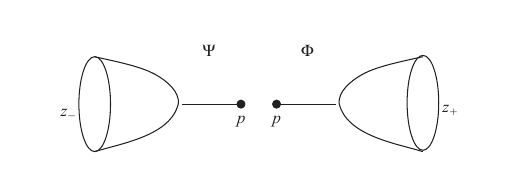
\includegraphics[width=.62\textwidth]{chapters/ch20-pants-product/figures/figure-20-1.png}
 \caption{PSS 映射 $\Psi$ 与 $\Phi$。}
 \label{fig:20-pss-maps}
\end{figure}

这里同样施加指标条件
\[
 \mu_{H_-}([z_-,w_-])=n-(\mu_{(-f)}(p)-2c_1(A_-)),
\]
使 $\mathcal M([z_-,w_-],p;A_-)$ 成为零维（可定向）流形。同样的延拓映射论证说明
$\Psi$ 是链映射，故在同调上诱导同态。

\stfhIndex{I028}{Jueretuihua}{绝热退化（adiabatic degeneration）}
\subsection{\personFloer{}模空间的绝热退化}

本小节描述 (OhZ11b) 建立的主要绝热粘合结果，不深入高度非平凡的分析细节；完整
细节见原文。在 $U_\pm$ 上用给定解析坐标 $z=e^{2\pi(\tau+it)}$，固定函数
\begin{equation}
 \kappa^+(\tau)=\begin{cases}0,&|\tau|\leq1,\\1,&|\tau|\geq2,
 \end{cases}
 \label{eq:20-kappa-plus}
\end{equation}
并令 $\kappa^-(\tau)=\kappa^+(-\tau)$。置
$\kappa_\epsilon^+(\tau)=\kappa^+(\tau-R(\epsilon)+1)$、
$\kappa_\epsilon^-(\tau)=\kappa_\epsilon^+(-\tau)$。容易看出
\begin{equation}
 \kappa_\epsilon^+(\tau)=\begin{cases}
 1,&\tau\geq R(\epsilon)+1,\\0,&\tau\leq R(\epsilon),
 \end{cases}
 \qquad
 \kappa_\epsilon^-(\tau)=\begin{cases}
 1,&\tau\leq-R(\epsilon)-1,\\0,&\tau\geq-R(\epsilon).
 \end{cases}
 \label{eq:20-kappa-epsilon-pm}
\end{equation}
再把它们在坐标卡 $U_\pm$ 外延拓为零。选取 $R=R(\epsilon)$，使
\begin{equation}
 \epsilon R(\epsilon)\longrightarrow0\qquad(\epsilon\to0).
 \label{eq:20-epsilon-r-normalization}
\end{equation}
绝热退化论证中的归一化步骤将用到这一选取。

还取截断函数 $\kappa_\epsilon^0:\mathbb R\to[0,1]$，满足
\begin{equation}
 \kappa_\epsilon^0(\tau)=\begin{cases}
 1,&|\tau|\leq R(\epsilon)-1,\\0,&|\tau|\geq R(\epsilon),
 \end{cases}
 \label{eq:20-kappa-zero}
\end{equation}
以及
\begin{equation}
 |(\kappa_\epsilon^0)'(\tau)|\leq2
 \qquad\text{当 }R(\epsilon)-1\leq|\tau|\leq R(\epsilon).
 \label{eq:20-kappa-derivative}
\end{equation}
考虑偶对 $(K_\epsilon,J_\epsilon)$ 的单参数族，其圆柱端为
\[
 \operatorname{End}_\pm(K_\epsilon,J_\epsilon)=(H,J),
 \qquad R_0\leq R(\epsilon)<\infty,
\]
其中 $(H,J)$ 是给定的\termFloerRegular{}偶对，具体如下。定义
\begin{equation}
 J_\epsilon(\tau,t,x)=\begin{cases}
 J^{\kappa_\epsilon^+(\tau)}(t,x),&\tau\geq R(\epsilon),\\
 J_0(x),&|\tau|\leq R(\epsilon)-1,\\
 J^{\kappa_\epsilon^-(\tau)}(t,x),&\tau\leq-R(\epsilon),
 \end{cases}
 \label{eq:20-j-epsilon}
\end{equation}
\footnote{译者注：原书分段条件在
$R(\epsilon)-1<|\tau|<R(\epsilon)$ 留出未定义的过渡带，却紧接着断言该族光滑。
截断函数显然意在填充该带，但页内未给出唯一公式，故译文照录。}
由上述截断函数，这定义了 $M$ 上一个光滑的 $\mathbb R\times S^1$ 殆复结构族。
类似地，定义 $K_\epsilon:\mathbb R\times S^1\times M\to\mathbb R$ 为
\begin{equation}
 K_\epsilon(\tau,t,x)=\begin{cases}
 \kappa_\epsilon^+(\tau)H(t,x),&\tau\geq R(\epsilon),\\
 \kappa_\epsilon^0(\tau)\epsilon f(x),&|\tau|\leq R(\epsilon),\\
 \kappa_\epsilon^-(\tau)H(t,x),&\tau\leq-R(\epsilon).
 \end{cases}
 \label{eq:20-k-epsilon}
\end{equation}

\begin{remark}
\label{rem:20-choice-k-epsilon}
\begin{enumerate}[label=(\arabic*)]
\item 定义 $K_\epsilon$ 时，我们使用线性同伦 $s\mapsto sH$；它由给定哈密顿量
$H=H(t,x)$ \emph{典范}确定。对任意同伦 $\mathcal H:s\mapsto H(s)$ 也可类似定义，其中
$H(s)=H(s,t,x)$ 是满足 $H(0)=\epsilon f$、$H(1)=H$ 的二参数族。所得同调映射与
同伦选取无关。
\item 比较上述 $K_\epsilon$ 与 (PSS96, MSa04) 的选取：他们使用颈部区域上
$K_\epsilon\equiv0$ 的族；我们则在颈部放入小\personMorse{}函数 $\epsilon f$，并取
$\epsilon\to0$ 的绝热极限。若颈部 $K_\epsilon\equiv0$，则在 (PSS96, MSa04) 所述
粘合构造中，很难从极限恢复\personFloer{}流线随 $\epsilon\to0$ 退化成节点流线的过程。
另一方面，我们在极限节点处提供记住背景\personMorse{}函数的一阶喷注数据。
\end{enumerate}
\end{remark}

对给定截断函数 $\kappa=\{\kappa_+,\kappa_-\}$，使用这个单参数族 $(K_R,J_R)$，
考虑参数化模空间
\[
 \begin{aligned}
 \mathcal M^{\mathrm{para}}([z_-,w_-],[z_+,w_+];\{(K,J;\kappa)\})
 &=\bigcup_{0<\epsilon\leq\epsilon_0}\{\epsilon\}\times
 \mathcal M([z_-,w_-],[z_+,w_+];K_\epsilon,J_\epsilon).
 \end{aligned}
\]
也简记 $\mathcal M^{\mathrm{para}}=\bigcup_{0<\epsilon\leq\epsilon_0}\mathcal M^\epsilon$。
为研究同调上的 $\Psi\circ\Phi$，需要分析 $\mathcal M^{\mathrm{para}}$ 的紧化。

以下关键分析定理完成 (Pi94), (PSS96) 所述 PSS 映射同构性质所需的论证。

\begin{theorem}[{(OhZ11b) 的定理 10.19}]
\label{thm:20-adiabatic-gluing}
令 $(K_\epsilon,J_\epsilon)$ 为~\eqref{eq:20-k-epsilon} 中定义的\personFloer{}数据族，则：
\begin{enumerate}[label=(\arabic*)]
\item 在
$\mathcal M^{\mathrm{para}}_{(0;1,1)}([z_-,w_-],[z_+,w_+];\{(K_\epsilon,J_\epsilon)\})$
上存在一种拓扑，使粘合构造对充分小的 $\epsilon_0$ 定义真嵌入
\[
 \begin{aligned}
 \operatorname{Glue}:{}&(0,\epsilon_0)\times
 \mathcal M^{\mathrm{nodal}}_{(0;1,1)}
 ([z_-,w_-],[z_+,w_+];(H,J),(f,J_0))\\
 &\longrightarrow
 \mathcal M^{\mathrm{para}}_{(0;1,1)}
 ([z_-,w_-],[z_+,w_+];\{(K,J)\}).
 \end{aligned}
\]
\item 上述拓扑可紧化为
$\overline{\mathcal M}^{\mathrm{para}}_{(0;1,1)}$，且作为集合
\[
 \overline{\mathcal M}^{\mathrm{para}}_{(0;1,1)}
 =\bigcup_{0<\epsilon\leq\epsilon_0}\{\epsilon\}\times
 \mathcal M_{(0;1,1)}(K_\epsilon,J_\epsilon)
 \ \cup\ \mathcal M^{\mathrm{nodal}}_{(0;1,1)}((H,J),(f,J_0)).
\]
\item 嵌入 $\operatorname{Glue}$ 光滑延拓为 $[0,\epsilon_0)$ 上的嵌入
$\overline{\operatorname{Glue}}$，满足
\[
 \overline{\operatorname{Glue}}(u_+,u_-,u_0;0)=\operatorname{Glue}(u_+,u_-,u_0).
\]
\end{enumerate}
\end{theorem}

完整证明见 (OhZ11b)。

\begin{figure}[htbp]
 \centering
 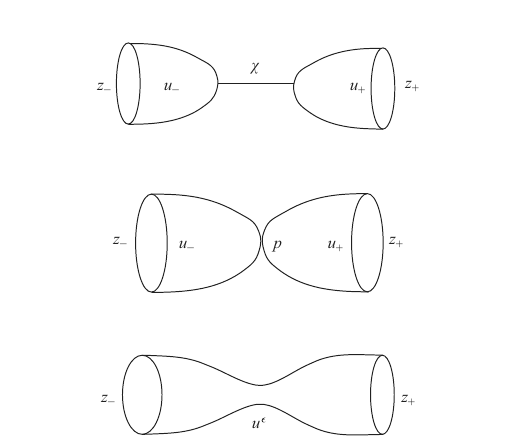
\includegraphics[width=.62\textwidth]{chapters/ch20-pants-product/figures/figure-20-2.png}
 \caption{PSS 方案。}
 \label{fig:20-pss-scheme}
\end{figure}

\subsection{证明的 PSS 方案}

\stfhIndex{I153}{Piwunixin-Salameng-Shiwaci}{皮乌尼欣--萨拉蒙--施瓦茨（Piunikhin--Salamon--Schwarz）}
本小节概述\personPiunikhin{}、\personSalamon{}和\personSchwarz{}对 PSS 映射同构性质的论证；它基于一个
形变，把复合映射
\[
 \Phi\circ\Psi:CF_*(H_+)\longrightarrow CF_*(H_+)
\]
与恒等映射之间建立链同伦。形变过程中涉及三类模空间（见图~\ref{fig:20-pss-scheme}）：
\footnote{译者注：原书此处称形变导向复合映射与恒等映射之间的“chain
isomorphism”，但随后构造的是链同伦并明确写出链同伦公式；译文据此写作“链同伦”。}
\begin{samepage}
\begin{enumerate}[label=(\arabic*)]
\item 圆盘--流--圆盘；
\item 节点\personFloer{}流线；
\item 链映射\personFloer{}流线。
\end{enumerate}
\end{samepage}

以下以 $\lambda\in[-1,1]$ 表示形变参数，使节点位形出现在 $\lambda=0$。只要
$\lambda>0$ 或 $\lambda<0$，形变所涉及的模空间类型相同，故标准论证分别在
$[-1,-\epsilon_0]$ 和 $[\epsilon_0,1]$ 上构造配边。要把配边延拓到整个区间，需要
用 $[-\epsilon_0,\epsilon_0]$ 上的配边连接二者。然而，模空间在 $\lambda=0$ 发生
“相变”，所以先验地只能期望得到\emph{分片光滑}配边；必须证明
$\mathcal M_0\subset\mathcal M^{\mathrm{para}}$ 的\emph{双领口定理}，才能实现 PSS 方案。
从 $-\epsilon_0$ 到 $0$ 的左单侧领口可由有限维构造得到（见 (OhZ11b) 第 9 节）；
$[0,\epsilon_0]$ 上右单侧领口的构造是非平凡的，它基于定理~\ref{thm:20-adiabatic-gluing}，
其证明使用 (OhZ11b) 的绝热退化方法。

应用定理~\ref{thm:20-adiabatic-gluing}，并逐字重复 (OhZ11b) 的论证（该论证又大体
沿用 (PSS96)），可证明下述 (PSS96) 中的同构性质。

\begin{theorem}
\label{thm:20-pss-one-sided-inverse}
令 $(-f;g)$ 为 $M$ 上\personMorse{}函数 $f$ 与度量 $g$ 的通有\personMorse{}--\personSmale{}偶对，
$H^{\mathrm{Morse}}(-f;g)$ 为其\personMorse{}同调。令 $(H,J)$ 为通有的含时周期哈密顿量
$H$ 与 $M$ 上相容殆复结构族 $J=\{J_t\}$。设 $\Psi,\Phi$ 为 (PSS96) 中的 PSS
映射。则存在同态
\[
 \Upsilon_{\mathrm{PSS}}:CF_*(H,J)\longrightarrow CF_{*+1}(H,J)
\]
满足
\begin{equation}
 \Phi\circ\Psi-\operatorname{id}
 =\partial_{(H,J)}\circ\Upsilon_{\mathrm{PSS}}
 -\Upsilon_{\mathrm{PSS}}\circ\partial^{\mathrm{Morse}}_{(-f,g)}.
 \label{eq:20-pss-chain-homotopy}
\end{equation}
\footnote{译者注：原书此式两项之间为减号；本节稍后的链同伦公式却使用加号。
这可能涉及作者的边界算子符号约定，也可能是排印不一致。此外，原书第二项使用
$\partial^{\mathrm{Morse}}_{(-f,g)}$，但 $\Upsilon_{\mathrm{PSS}}$ 的定义域和值域均为
$CF_*(H,J)$，故该复合在类型上也不成立；译文两处均照录。}
特别地，在同调上 $\Phi_*\circ\Psi_*=\operatorname{id}$。
\end{theorem}

这说明 $\Phi_*\circ\Psi_*=\operatorname{id}$。另一个恒等式
$\Psi_*\circ\Phi_*=\operatorname{id}$ 更容易证明；细节见 (OhZ11b) 第 9 节。

\begin{remark}
\label{rem:20-one-jet-datum}
\personFloer{}流线方程解模空间带中部\personMorse{}函数 $\epsilon f$ 的绝热退化，不仅产生 PSS 方案所用
的节点\personFloer{}流线，还产生带一阶喷注数据的节点\personFloer{}流线；该数据反映背景\personMorse{}函数 $f$ 的存在。这在 (OhZ11b) 的尺度依赖粘合中至关重要。
\end{remark}

\subsection{\texorpdfstring{$\Phi_*\circ\Psi_*=\operatorname{id}$}{Phi o Psi = id}：从\personFloer{}经\personMorse{}回到\personFloer{}}

考虑定义在 $\kappa\in[-\infty,1]$ 上的 PSS 形变。固定通有同伦
$(K^\kappa,J^\kappa)$，其中
$K^\kappa=K^\kappa(\tau,t,x)$、$J^\kappa=J^\kappa(\tau,t,x)$，它从
$(K^{\epsilon_0},J^{\epsilon_0})$ 连接到
$(K^1(\tau,t,x),J^1(\tau,t,x))=(H(t,x),J(t,x))$。
固定充分小的 $\epsilon_0>0$ 与充分大的 $\ell_0>0$，把形变分成四段：
\[
 \begin{array}{ll}
 (K^\kappa,J^\kappa),&\epsilon_0\leq\kappa\leq1,\\
 (K_\epsilon,J_\epsilon),&0<\kappa=\epsilon\leq\epsilon_0,\\
 (H^{\rho_-},J^{\rho_-})_{o_-}*(-f,g_{J_0};[-\ell,\ell])_{*_{o_+}}
 (H^{\rho_+},J^{\rho_+}),&-\ell_0\leq\ell<0,\\
 (H^{\rho_-},J^{\rho_-})_{o_-}*(-f,g_{J_0};[-\ell,\ell])_{*_{o_+}}
 (H^{\rho_+},J^{\rho_+}),&-\infty\leq\ell<-\ell_0.
 \end{array}
\]
这里 $(f,J_0;[-\ell,\ell])$ 表示形变
\[
 \ell\in(-\infty,0)\longmapsto(-f,g_{J_0};[-\ell,\ell]),
\]
其中 $f$ 是相对于度量 $g_{J_0}$ 的\personMorse{}函数，我们考虑其在区间
$[-\ell,\ell]$ 上的梯度流线。

以 $\mathcal M_\kappa^{\Psi\Phi}([z_-,w_-],[z_+,w_+])$ 表示对应参数 $\kappa$ 的
位形模空间，以参数化模空间表示整个形变：
\[
 \overline{\mathcal M}_{\Psi\Phi}^{\mathrm{para}}
 ([z_-,w_-],[z_+,w_+];f)
 =\bigcup_{\kappa\in[-1,\infty]}
 \mathcal M_\kappa^{\Psi\Phi}([z_-,w_-],[z_+,w_+]).
\]
\footnote{译者注：本小节开头把参数域写作 $[-\infty,1]$，此处却反向写作
$[-1,\infty]$；随后各段又使用负无穷端与上端 $1$，故两处不能同时成立。译文照录。}
由非退化假设和指标条件，除有限多个点外 $\mathcal M_\kappa^{\Psi\Phi}$ 为空；这些点
位于
\[
 \kappa\in(-\ell_0,-\ell_1)\cup(\epsilon_0,1).
\]
先验地，当 $\kappa\to0$ 时它们可能在 $[-\ell_1,\epsilon_0]$ 内聚集。但对应
$\kappa=0$ 的加强节点\personFloer{}流线模空间的一阶喷注横截性，以及
定理~\ref{thm:20-adiabatic-gluing} \emph{排除}了这种聚集。因此，若取 $\ell_1,\epsilon_0$
充分小，则对所有 $\kappa\in[-\ell_1,\epsilon_0]$ 有
\[
 \mathcal M_\kappa^{\Psi\Phi}([z_-,w_-],[z_+,w_+])=\varnothing.
\]
结合主要粘合紧性结果和定理~\ref{thm:20-adiabatic-gluing}，得到：

\begin{proposition}
\label{prop:20-phi-psi-compactification}
存在常数 $\ell_0,\ell_1,\epsilon_0,\epsilon_1$，使：
\begin{enumerate}[label=(\arabic*)]
\item 若 $\mu_H([z_-,w_-])-\mu_H([z_+,w_+])=-1$，则
$\overline{\mathcal M}_{\Psi\Phi}^{\mathrm{para}}([z_-,w_-],[z_+,w_+])$
是紧零维流形，并且当
$\kappa\in[-\infty,-\ell_0]\cup[-\ell_1,\epsilon_0]\cup[1-\epsilon_1,1]$
时 $\mathcal M_\kappa^{\Psi\Phi}=\varnothing$。
\item 若指标差为 $0$，则
$\overline{\mathcal M}_{\Psi\Phi}^{\mathrm{para}}([z_-,w_-],[z_+,w_+];f)$
是紧一维流形，其边界为
\[
 \begin{aligned}
 \partial\overline{\mathcal M}_{\Psi\Phi}^{\mathrm{para}}
 &=\mathcal M_{\kappa=1}([z_-,w_-],[z_+,w_+])
 \cup\mathcal M_{-\infty}([z_-,w_-],[z_+,w_+])\\
 &\quad\cup\bigcup_{[z,w]}
 \overline{\mathcal M}_{\Psi\Phi}^{\mathrm{para}}([z_-,w_-],[z,w])
 \#\mathcal M_{\kappa=1}([z,w],[z_+,w_+])\\
 &\quad\cup\bigcup_{[z,w]}
 \mathcal M_{\kappa=1}([z_-,w_-],[z,w])
 \#\overline{\mathcal M}_{\Psi\Phi}^{\mathrm{para}}([z,w],[z_+,w_+]),
 \end{aligned}
\]
第一、第二个并分别遍历满足相应指标差为 $-1$ 的 $[z,w]$。
\end{enumerate}
\end{proposition}

命题 (1) 可定义阶数为
$\#\overline{\mathcal M}_{\Psi\Phi}^{\mathrm{para}}([z_-,w_-],[z_+,w_+];f)$
的矩阵系数，从而定义映射
\[
 \Upsilon_{\mathrm{PSS}}^{\Psi\Phi}:CF_*(H)\to CF_{*+1}(H),
\]
其矩阵系数为
\[
 \langle\Upsilon_{\mathrm{PSS}}^{\Psi\Phi}([z_-,w_-]),[z_+,w_+]\rangle
 =\#\overline{\mathcal M}_{\Psi\Phi}^{\mathrm{para}}([z_-,w_-],[z_+,w_+];f).
\]
命题 (2) 对一维模空间边界的描述转化为
\[
 \Phi\circ\Psi-\operatorname{id}
 =\partial\circ\Upsilon_{\mathrm{PSS}}^{\Psi\Phi}
 +\Upsilon_{\mathrm{PSS}}^{\Psi\Phi}\circ\partial.
\]
这完成了同调上 $\Phi_*\circ\Psi_*=\operatorname{id}$ 的证明。

\subsection{\texorpdfstring{$\Psi_*\circ\Phi_*=\operatorname{id}$}{Psi o Phi = id}：从\personMorse{}经\personFloer{}回到\personMorse{}}

对每一对 $p,q\in\operatorname{Crit}f$，考虑参数化模空间
\[
 \overline{\mathcal M}_{\Phi\Psi}^{\mathrm{para}}(p,q)
 =\bigcup_{0\leq R\leq\infty}\mathcal M_R^{\Phi\Psi}(p,q).
\]
定义如下。对每个 $0<R<\infty$，先引入方程
\begin{equation}
 \overline\partial_{(K^R,J^R)}u=0
 \label{eq:20-r-dependent-cr}
\end{equation}
在 $\Sigma$ 上的有限能量解模空间
$\mathcal M_{(2;0,0)}(K^R,J^R)$。这里 $\Sigma$ 是带两个标记点
$\{o_-,o_+\}$ 的\personRiemann{}曲面，满足
$\Sigma\setminus\{o_\pm\}\cong\mathbb R\times S^1$。先以连通和定义\personRiemann{}曲面族 $(\Sigma,j_R)$：
\[
 (D^-,o_-)\cup C_R\cup(D^+,o_+),\qquad
 j_R=j_{D^-}\#j_{C_R}\#j_{D^+},
\]
其中 $C_R=[-R,R]\times S^1$，$j_{C_R}$ 是标准共形结构，$j_R$ 是
$D^-\cup C_R\cup D^+$ 上显然的粘合共形结构。以 $(\tau,t)$ 表示
$D^-\cup C_R\cup D^+\setminus\{o_-,o_+\}$ 上延拓 $C_R$ 标准坐标的共形坐标。

在这些坐标中固定截断函数族
\[
 \chi^R(\tau)=\begin{cases}
 1-\kappa^+(\tau-R),&\tau\geq0,\\
 1-\kappa^-(\tau+R),&\tau\leq0,
 \end{cases}
\]
其中 $1\leq R<\infty$；对 $0\leq R\leq1$ 令 $\chi^R=R\chi^1$。注意
$\chi^0\equiv0$，$\chi^R$ 具有紧支集，并且对任意给定紧子集，当 $R$ 充分大时
$\chi^R\equiv1$。因此，方程~\eqref{eq:20-r-dependent-cr} 在标记点 $o_\pm$ 附近化为
$\overline\partial_{J_0}u=0$。如前定义 $(K^R,J^R)$。

有两个评价映射
\[
 \operatorname{ev}_{o_\pm}:\mathcal M_{(2;0,0)}(K^R,J^R)\to M,
 \qquad\operatorname{ev}_{o_\pm}(u)=u(o_\pm).
\]
记
\[
 \begin{aligned}
 \widetilde{\mathcal M}^-(p;f)
 &=\{\chi:\mathbb R\to M\mid\dot\chi+\nabla(-f)(\chi)=0,
 \ \chi(-\infty)=p\},\\
\widetilde{\mathcal M}^+(q;f)
&=\{\chi:\mathbb R\to M\mid\dot\chi+\nabla(-f)(\chi)=0,
 \ \chi(+\infty)=q\},
\end{aligned}
\]
\footnote{译者注：原书把以上两处映射的类型写成“$\chi:\mathbb R\times M$”，没有
给出值域；由微分方程及端点条件可知应为 $\chi:\mathbb R\to M$，译文据此补正。}
并定义
\[
 \widetilde{\mathcal M}_1^-(p;-f)=\widetilde{\mathcal M}^-(p;-f)\times\mathbb R,
 \qquad
 \widetilde{\mathcal M}_1^+(q;-f)=\widetilde{\mathcal M}^+(q;-f)\times\mathbb R.
\]
$\tau_0\in\mathbb R$ 通过
$(\tau_0,(\chi,\tau))\mapsto(\chi(*-\tau_0),\tau+\tau_0)$ 自由作用，故商
\[
 \mathcal M_1^-(p;-f)=\widetilde{\mathcal M}_1^-(p;-f)/\mathbb R,
 \quad
 \mathcal M_1^+(q;-f)=\widetilde{\mathcal M}_1^+(q;-f)/\mathbb R
\]
\footnote{译者注：原书先以参数“$f$”定义 $\widetilde{\mathcal M}^{\pm}(\cdot;f)$，
但方程已使用 $\nabla(-f)$；紧接着又把同一对象代入参数“$-f$”定义
$\mathcal M_1^{\pm}(\cdot;-f)$。若逐字代入会反转梯度号，故此处存在记号不一致；
译文保留原书记号。}
分别是维数 $\mu_{\mathrm{Morse}}(p;f)$ 与
$2n-\mu_{\mathrm{Morse}}(q;f)$ 的光滑流形。其渐近评价映射
\[
 \operatorname{ev}_+:\mathcal M_1^+(q;-f)\to M,
 \qquad \operatorname{ev}_-:\mathcal M_1^-(p;-f)\to M
\]
的像分别与不稳定流形 $W^u(p;-f)$ 和稳定流形 $W^s(q;-f)$ 一一对应。
\footnote{译者注：原书按 $\operatorname{ev}_+$、$\operatorname{ev}_-$ 的顺序列出
定义域 $\mathcal M_1^+(q;-f)$、$\mathcal M_1^-(p;-f)$，却说其像“分别”为
$W^u(p;-f)$、$W^s(q;-f)$；变量和稳定/不稳定流形均与该顺序不匹配。译文照录。}

定义 $\mathcal M_R^{\Phi\Psi}(p,q;A)$ 为\termFiberProduct{}
\[
 \begin{aligned}
 \mathcal M_R^{\Phi\Psi}(p,q;A)
 &=\mathcal M_1^-(p;-f)_{\operatorname{ev}_-}
 \times_{\operatorname{ev}_{o_-}}\mathcal M_{(2;0,0)}(K^R,J^R;A)\\
 &\qquad{}_{\operatorname{ev}_{o_+}}
 \times_{\operatorname{ev}_+}\mathcal M_1^+(q;-f)\\
 &=\{((\chi_-,\tau_-),u,(\chi_+,\tau_+))\mid
 \chi_-(\tau_-)=u(o_-),\ \chi_+(\tau_+)=u(o_+)\},
 \end{aligned}
\]
并令
\[
 \overline{\mathcal M}^{\Phi\Psi,\mathrm{para}}(p,q;A)
 =\bigcup_{0\leq R\leq\infty}\mathcal M_R^{\Phi\Psi}(p,q;A).
\]
直接计算得到
\[
 \dim^{\mathrm{virt}}\mathcal M_R^{\Phi\Psi}(p,q;A)
 =\mu_{\mathrm{Morse}}(p)-\mu_{\mathrm{Morse}}(q)+2c_1(A).
\]

\begin{proposition}
\label{prop:20-psi-phi-compactification}
取通有偶对 $(f,J_0)$，并令 $0<\epsilon_1<R_1$。
\footnote{译者注：原书在本命题开头先令 $0<\epsilon_1<R_1$，但第 (1) 项又说“存在
某个 $\epsilon_1>0$ 和 $R_1>0$”；证明末还写成相反的 $R_1\leq\epsilon_1$。这些
量词和不等式彼此不容，译文逐处照录。}
\begin{enumerate}[label=(\arabic*)]
\item 若 $\mu_{\mathrm{Morse}}(p)-\mu_{\mathrm{Morse}}(q)+2c_1(A)=-1$，
则存在某个 $\epsilon_1>0$ 与 $R_1>0$，使
$\overline{\mathcal M}^{\Phi\Psi,\mathrm{para}}(p,q;A)$ 是紧零维流形，并且当
$0\leq R\leq\epsilon_1$ 或 $R\geq R_1$ 时
$\mathcal M_R^{\Phi\Psi}(p,q;A)=\varnothing$。
\item 若上述指标为 $0$，则
$\overline{\mathcal M}^{\Phi\Psi,\mathrm{para}}(p,q;A)$ 是紧一维流形，其边界为
\[
 \partial\overline{\mathcal M}^{\Phi\Psi,\mathrm{para}}(p,q;A)
 =\mathcal M_0^{\Phi\Psi}(p,q;A)\cup\mathcal M_\infty^{\Phi\Psi}(p,q;A)
 \cup\bigcup_r\overline{\mathcal M}^{\Phi\Psi}(p,r;A),
\]
\footnote{译者注：原书边界式最后一项只含 $(p,r;A)$，使原先固定的输出 $q$ 消失；
若它描述\personMorse{}破裂，通常还应出现从 $r$ 到 $q$ 的因子。页内资料不足以唯一补全，
译文照录。}
其中最后的并遍历满足
$\mu_{\mathrm{Morse}}(p)-\mu_{\mathrm{Morse}}(r)+2c_1(A)=-1$ 的
$r\in\operatorname{Crit}(-f)$。
\end{enumerate}
\end{proposition}

\begin{proof}
当 $R=0$ 时，方程~\eqref{eq:20-r-dependent-cr} 化为
$\overline\partial_{J_0}u=0$。因为
$\mu_{\mathrm{Morse}}(p)-\mu_{\mathrm{Morse}}(q)+2c_1(A)=-1$ 是
$\mathcal M_0^{\Phi\Psi}(p,q;A)$ 的虚维数，对通有 $(f,J_0)$ 该空间必为空。这里强调，
此模空间只依赖 $(f,J_0)$，故通有性论证可与参数 $R$ 无关地应用。因此当
$R_1\leq\epsilon_1$ 且 $\epsilon_1>0$ 充分小时，同样成立。证明完毕。第 (2) 项留给
读者。
\end{proof}

由 (1) 定义链同伦映射
\[
 \Upsilon_{\mathrm{PSS}}^{\Phi\Psi}:
 CM_*(-f,g_{J_0};\Lambda_\omega)\to CM_{*+1}(-f,g_{J_0};\Lambda_\omega),
\]
其矩阵元为
\[
 \langle\Upsilon_{\mathrm{PSS}}^{\Phi\Psi}(p),q\#(-A)\rangle
 =\sum_{(r,A)}\#\left(\bigcup_r
 \overline{\mathcal M}^{\Phi\Psi,\mathrm{para}}(p,r;A)\right).
\]
\footnote{译者注：原书左端固定 $q$，右端却对 $(r,A)$ 求和又在括号内再对 $r$ 取并，
同时复用 $A$；该矩阵元的下标无法由页内资料唯一重构，译文照录。}

\begin{lemma}
\label{lem:20-zero-end-dimension}
设 $\mu_{\mathrm{Morse}}(p)-\mu_{\mathrm{Morse}}(q)+2c_1(A)=0$。若 $A\neq0$，则除非
$\mathcal M_0^{\Phi\Psi}(p,q;A)=\varnothing$，否则
\[
 \dim\mathcal M_0^{\Phi\Psi}(p,q;A)\geq2.
\]
当 $A=0$ 时，除非 $p=q$，否则
\[
 \dim\mathcal M_0^{\Phi\Psi}(p,q;A)\geq1.
\]
\end{lemma}

\begin{proof}
若 $A\neq0$，则 $(u;o_-,o_+)\in\mathcal M_{(2;0,0)}(K^R,J^R)$ 中的 $u$ 非常值。
定义域 $(\Sigma;o_-,o_+)$ 的共形自同构产生至少实二维族，与指标假设矛盾（半正
情形见 (Fl89b), (FHS95)，一般情形见 (FOn99), (LT98)）。

若 $A=0$，任何 $J_0$-全纯球面都为常值，相应位形
$(\chi_-,\text{常值},\chi_+)$ 因而成为完整梯度流线
$\chi=\chi_-\#\chi_+$。除非 $\chi$ 为常值（即 $p=q$），否则 $\mathbb R$-平移产生
至少一维族，再次与指标假设矛盾。
\end{proof}

现在可完成恒等式
\begin{equation}
 \Psi\circ\Phi-\operatorname{id}
 =\Upsilon_{\mathrm{PSS}}^{\Phi\Psi}\partial^{\mathrm{Morse}}_{(-f,g_{J_0})}
 +\partial^{\mathrm{Morse}}_{(-f,g_{J_0})}\Upsilon_{\mathrm{PSS}}^{\Phi\Psi}
 \label{eq:20-psi-phi-chain-homotopy}
\end{equation}
的证明。先验地，命题~\ref{prop:20-psi-phi-compactification} 只给出
\[
 \sum_{q,A}\langle(\Psi\circ\Phi-\operatorname{id})(p),q\#(-A)\rangle
 =\sum_{q,A}\left\langle
 \Upsilon_{\mathrm{PSS}}^{\Phi\Psi}\partial^{\mathrm{Morse}}_{(-f,g_{J_0})}(p)
 +\partial^{\mathrm{Morse}}_{(-f,g_{J_0})}\Upsilon_{\mathrm{PSS}}^{\Phi\Psi}(p),
 q\#(-A)\right\rangle.
\]
但上述引理蕴含
\[
 \langle(p),q\#(-A)\rangle=0,
\]
除非 $A=0$ 且 $p=q$。这便证明了~\eqref{eq:20-psi-phi-chain-homotopy}。

\stfhIndex{I092}{Fuluobeiniwusipeidui}{弗罗贝尼乌斯配对（Frobenius pairing）}
\section{\personFrobenius{}配对与对偶性}
\label{sec:frobenius-pairing-duality}

回忆~\eqref{eq:20-flat-qh}、\eqref{eq:20-sharp-qh} 中给出的同构
$\flat:QH^*(M)\to QH_*(M)$ 及其逆
$\sharp:QH_*(M)\to QH^*(M)$。仍分别以 $a^\flat,b^\sharp$ 表示这些映射下的像。

\begin{definition}[\personFrobenius{}配对]
\label{def:20-frobenius-pairing}
定义非退化配对
\begin{equation}
 \Delta=\langle\cdot,\cdot\rangle:
 QH^k(M)\otimes QH^{n-k}(M)\longrightarrow\Lambda_\omega^{(0)}
 \label{eq:20-frobenius-pairing}
\end{equation}
为
\begin{equation}
 \left\langle\sum_Aa_Aq^A,\sum_Bb_Bq^B\right\rangle
 =\sum_{C;\,c_1(C)=0}\left(\sum_A(a_A,b_{C-A})\right)q^C,
 \label{eq:20-frobenius-coefficients}
\end{equation}
其中 $(a_A,b_B)$ 是 $H^k(M,\mathbb Q)$ 与 $H_k(M,\mathbb Q)$ 之间的典范\personPoincare{}配对：
\[
 (a_A,b_B)=a_A\cap PD(b_B).
\]
\footnote{译者注：原书把第二因子的次数印作 $n-k$，而本书以 $\dim M=2n$，且本段
随即把 $H^k$ 与 $H_k$ 配对；通常的上同调\personPoincare{}配对应涉及 $2n-k$。原书在
命题 20.4.4 又重复 $n-k$，故译文照录并登记此疑点。}
由 $QH^*(M)$ 定义中的有限性条件，式~\eqref{eq:20-frobenius-coefficients} 的和总是
有限的，因而定义良好。
\end{definition}

\begin{proposition}
\label{prop:20-frobenius-cup}
以 $[M]$ 表示基本类，以 $1=PD[M]$ 表示 $QH^*(M)$ 的单位元。则
\[
 \langle a,b\rangle=(a\cup_Qb)\cap[M]=\langle(a\cup_Qb),1\rangle.
\]
\end{proposition}

\begin{proof}
只需对上同调类 $a,b\in H^*(M)$ 证明第一个等式。这时左端就是经典\personPoincare{}对偶配对
\[
 (a_A,b_{C-A})=a_A\cap PD(b_{C-A})=(a_A\cup b_{C-A})\cap[M].
\]
现计算右端。以闭链 $P_1,P_2$ 代表 $PD(a),PD(b)$。依定义，
$(a\cup_Qb)\cap[M]$ 位于 $H_0(M;\Lambda_\omega)\cong\Lambda_\omega$，由
\[
 \sum_{\alpha\in\pi_2(M)}
 \mathcal M_3(J_0;\alpha)_{(\operatorname{ev}_1,\operatorname{ev}_2,
 \operatorname{ev}_0)}\times(P_1\times P_2\times M)
 T^{\omega(\alpha)}e^{c_1(\alpha)}
\]
给出，其中 $c_1(\alpha)=0$，故
$(a\cup_Qb)\cap[M]\in\Lambda_\omega^{(0)}\subset\Lambda_\omega$。

另一方面，\termFiberProduct{}
$\mathcal M_3(J_0;\alpha)_{(\operatorname{ev}_1,\operatorname{ev}_2,
\operatorname{ev}_0)}\times(P_1\times P_2\times M)$ 定义一个包含在
$C_0(M;\mathbb Q)$ 中的闭链，故维数必须为零。这只有在 $\alpha=0$ 时才可能；
于是 $\mathcal M_3(J_0;\alpha)$ 的所有元素都是常值映射，否则模空间的维数必须至少
有两个实维数，对应第零个标记点 $z_0$ 的变化。注意，由于 $M$ 是整个空间，对
$z_0$ 没有限制，因此可自由移动 $z_0$ 而不影响映射，也不影响在标记点 $z_1,z_2$
处分别与 $P_1,P_2$ 的给定相交。这证明上述\termFiberProduct{}恰好化为经典帽积
$(a\cup_Qb)\cap[M]=(a,b)$。
\end{proof}

定义 $\mathbb Q$-双线性配对 $\Pi$：
\begin{equation}
 \Pi(a,b)=\pi_0\circ\Delta(a,b)=\pi_0(\langle a\cdot b,1\rangle),
 \label{eq:20-rational-pairing}
\end{equation}
其中 $\pi_0:\Lambda_{0,\omega}\to\mathbb Q$ 是显然的投影，
$\pi_0(\sum_Aa_Aq^A)=a_{A=0}$。

\begin{remark}
\label{rem:20-continuous-dual}
即使作为 $\mathbb Q$-向量空间，$QH_*(M)$ 的对偶向量空间 $(QH_*(M))^*$ 也\emph{不同构}于
标准量子上同调 $QH^*(M)$。上述配对实际诱导单射
\[
 QH^*(M)\lhook\joinrel\longrightarrow(QH_*(M))^*,
\]
其像位于 $QH_*(M)$ 上的\emph{连续}线性泛函集合中；这里连续性相对于
式~\eqref{eq:20-downward-valuation} 的\termValuation{} $v$ 所诱导的拓扑而言。
\end{remark}

\begin{proposition}
\label{prop:20-pi-nondegenerate}
$\Pi$ 非退化。换言之，若对所有 $b\in QH^{n-k}(M)$ 都有 $\Pi(a,b)=0$，则 $a=0$。
\end{proposition}

\begin{proof}
若 $\Pi(a,b)=0$，则 $\pi_0(\Delta(a,b))=0$，故
\[
 \sum_{C;\,c_1(C)=\omega(C)=0}\sum_A(a_A,b_{C-A})=0.
\]
但 $c_1(C)=\omega(C)=0$ 蕴含 $C=0$ 于 $\Gamma$，因此对所有
$b_{-A}\in H^{n-k}(M)$ 都有 $\sum_{A\in\Gamma}(a_A,b_{-A})=0$。若
$a\in QH^k(M)$，取 $b=a_{-A}q^{-A}$，其中 $a_{-A}\in QH^{n-k}(M)$，便证明
对所有 $A\in\Gamma$ 都有 $a_A=0$，故 $a=0$。
\footnote{译者注：原书直接取 $b=a_{-A}q^{-A}$，却未说明为何系数 $a_{-A}$ 同时
属于互补次数，亦未取与 $a_A$ 配对非零的\personPoincare{}对偶元素；此处类型与非退化性
论证均有缺口。译文照录。}
\end{proof}

在第 22.5.1 小节中，我们将把 $QH^*(M)$ 看成小\personMorse{}函数的\personFloer{}上同调，利用
$QH^*(M)$ 与 $HF_*(H)$ 之间的自然同构，进一步研究\personFrobenius{}配对
\eqref{eq:20-frobenius-pairing}、\personFloer{}复形配对 (19.7.49) 以及二者的关系。


\chapter{谱不变量：构造}
\label{ch:spectral-construction}

为系统解释埃利亚什伯格的 $C^0$ 辛刚性结果，维泰博 (Vi92) 考察紧支哈密顿
微分同胚 $\phi$ 的图像，构造了 $\mathbb R^{2n}$ 上的一族辛不变量。他沿
$\mathbb R^{4n}=\mathbb R^{2n}\times\mathbb R^{2n}$ 的对角方向将此图像紧化到
$T^*S^{2n}$ 中，再把拉格朗日子流形 $\operatorname{graph}\phi\subset T^*S^{2n}$
的生成函数临界点理论以及任意闭光滑流形 $N$ 的余切丛 $T^*N$ 上的“稳定莫尔斯
理论”应用于它。当拉格朗日子流形 $L$ 带有生成函数时——例如 $L$ 与 $T^*N$ 的
零截面哈密顿同痕时——维泰博对每个上同调类 $a\in H^*(N)$ 都从给定生成函数
关联一个同调本质的临界值，并证明至少在相差归一化的意义下，它们只依赖于
拉格朗日子流形而不依赖于生成函数。

温斯坦观察到，作用量泛函是定义在给定哈密顿量 $H$ 的流把零截面送到
$\phi_H^1(o_N)$ 所对应道路空间上的生成函数。利用这一观察，笔者在 (Oh97b,
Oh99) 中发展了作用量泛函极小极大理论的弗洛尔理论方法，并构造出一族同样由
$H^*(N)$ 参数化的辛不变量，称为\emph{拉格朗日谱不变量}。此方法\emph{连同归一化}都是典范的，
并以透明的方式直接联系霍费尔几何与维泰博不变量。随后\personMilinkovic{}与笔者
证明，这族谱不变量在模掉归一化后确与维泰博不变量一致 (MiO95, Mi00)。

施瓦茨 (Schw00) 把类似方案用于\emph{辛非球面}的 $(M,\omega)$ 上的哈密顿不动点
弗洛尔理论；这里辛非球面意指
$c_1|_{\pi_2(M)}=\omega|_{\pi_2(M)}=0$。他由此得到一族由 $H^*(M)$ 参数化的
类似不变量。尤其是，他证明了谱不变量的重要最优三角不等式；在 (Oh97b, Oh99)
写作之时，上述拉格朗日谱不变量尚缺少这一结果。最近，\personMonzner{}、\personVichery{}与\personZapolsky{}也为拉格朗日谱不变量建立了相似的最优三角不等式 (MVZ12)。

在非正合辛流形上，作用量泛函不是单值的；弗洛尔同调理论须作为圆周值莫尔斯
理论，或作为可缩自由环路空间 $\mathcal L_0(M)$ 的覆盖空间
$\widetilde{\mathcal L}_0(M)$ 上的莫尔斯理论来发展。此时弗洛尔理论包含量子
效应，并本质地使用诺维科夫环。量子效应的出现，以及非有理辛流形上作用谱在
$\mathbb R$ 中的\emph{稠密性}，一直是研究\emph{哈密顿微分同胚族}时最严重的障碍。笔者继而在
(Oh02, Oh05c) 中，通过覆盖空间 $\widetilde{\mathcal L}_0(M)$ 上的链层弗洛尔
理论发展了一般的极小极大理论，并为每个给定的含时哈密顿量 $H$ 关联一族谱
不变量。此时这族不变量由量子上同调 $QH^*(M)$ 参数化，现在称为\emph{哈密顿谱不变量}。

\section{能量估计与霍费尔几何}
\label{sec:energy-estimates-hofer-geometry}

本节考察各种弗洛尔算子，以及它们如何改变复形 $CF^\lambda$ 的滤过层级。

固定哈密顿量 $H_\alpha,H_\beta$ 以及二者之间的同伦
$\mathcal H$。要强调的是，本节讨论中 $H_\alpha,H_\beta$ \emph{未必}非退化。选取相容殆复
结构的同伦 $j=\{J(\eta)\}_{0\leq\eta\leq1}$ 及截断函数
$\rho:\mathbb R\to[0,1]$，考虑相应弗洛尔方程
\begin{equation}
 \begin{cases}
 \partial u/\partial\tau+J^\rho
 (\partial u/\partial t-X_{H^\rho}(u))=0,\\
 u(-\infty)=z^-,\quad u(\infty)=z^+.
 \end{cases}
 \label{eq:21-floer-homotopy}
\end{equation}
下面的能量估计是联系作用量积分、弗洛尔连接流线的能量以及相应哈密顿量的霍费尔
范数的关键估计。它是命题~\ref{prop:20-energy-curvature-identity} 的特殊情形。这里给出一个
直接证明；在此特殊情形中它也颇具启发性，是引理 14.4.5 证明的一个变形。

\begin{proposition}
\label{prop:21-basic-energy-estimate}
设 $H_\alpha,H_\beta$ 是任意哈密顿量，不要求非退化；令
$\mathcal H=\{H^s\}_{0\leq s\leq1}$ 是二者之间的同伦。考虑对子
$(\mathcal H,j)$，并令 $\rho$ 是如前的任意截断函数。设 $u$ 满足
\eqref{eq:21-floer-homotopy}、$w^-\#u\sim w^+$（见 (19.4.16)），具有有限能量，
且对某些满足 $\tau_j^-\to-\infty,\tau_j^+\to\infty$ 的序列 $\tau_j^\pm$ 有
\[
 \lim_{j\to\infty}u(\tau_j^-)=z^-,\qquad
 \lim_{j\to\infty}u(\tau_j^+)=z^+.
\]
则\footnote{译者注：本命题只引入了端点哈密顿量 $H_\alpha,H_\beta$，原式却改用
$H,F$ 而未显式说明对应关系；译文照录原式记号。}
\begin{align}
 \mathcal A_F([z^+,w^+])-\mathcal A_H([z^-,w^-])
 &=-\int_{-\infty}^{\infty}\!\int_0^1
 \left\lVert\frac{\partial u}{\partial\tau}\right\rVert_{J^{\rho(\tau)}}^2
 \,dt\,d\tau \notag\\
 &\quad-\int_{-\infty}^{\infty}\rho'(\tau)\int_0^1
 \left.\frac{\partial H^s}{\partial s}\right|_{s=\rho(\tau)}
 (t,u(\tau,t))\,dt\,d\tau.
 \label{eq:21-action-energy-identity}
\end{align}
\end{proposition}

\begin{proof}
由同伦条件 $w^-\#u\sim w^+$，有
\[
 \int u^*\omega=\int(w^+)^*\omega-\int(w^-)^*\omega.
\]
更一般地，
\[
 \int_{w^-\#(u|_{-\infty<\tau'\leq\tau})}\omega
 =\int(w^-)^*\omega-\int_{-\infty}^{\tau}\!\int_0^1u^*\omega\,d\tau.
\]
为简化记号，以 $u(\tau)$ 表示环路 $t\mapsto u(\tau,t)$。若记
\[
 \widetilde u(\tau)=
 [u(\tau),w^-\#(u|_{-\infty<\tau'\leq\tau})],
\]
则
\[
 \mathcal A_F([z^+,w^+])-\mathcal A_H([z^-,w^-])
 =\int_{-\infty}^{\infty}\frac d{d\tau}
 \bigl(\mathcal A_{H^{\rho(\tau)}}(\widetilde u(\tau))\bigr)\,d\tau.
\]
计算得
\[
 \frac d{d\tau}\mathcal A_{H^{\rho(\tau)}}(\widetilde u(\tau))
 =d\mathcal A_{H^{\rho(\tau)}}(u(\tau))
 \left(\frac{\partial u}{\partial\tau}\right)
 -\int_0^1\frac{\partial H^{\rho(\tau)}}{\partial\tau}
 (\widetilde u(\tau,t))\,dt.
\]
这里 $d\mathcal A_{H^{\rho(\tau)}}(\widetilde u(\tau))$ 是固定 $\tau$ 后，哈密顿量
$H^{\rho(\tau)}=H^{\rho(\tau)}(t,x)$ 的作用量泛函在 $\widetilde u(\tau)$ 处的微分。
方程~\eqref{eq:21-floer-homotopy} 也是该含 $\tau$ 作用量泛函的负梯度流方程，故右端为
\[
 -\int_0^1\left\lVert\frac{\partial u}{\partial\tau}\right\rVert_{J_t^{\rho(\tau)}}^2dt
 -\rho'(\tau)\int_0^1
 \left.\frac{\partial H^s}{\partial s}\right|_{s=\rho(\tau)}
 (u(\tau,t))\,dt.
\]
在 $\tau\in\mathbb R$ 上积分即得~\eqref{eq:21-action-energy-identity}，证明完毕。
\end{proof}

现在从~\eqref{eq:21-action-energy-identity} 推出两条渐近轨道之间作用量差的各种结论。
先考察边界映射方程 (18.5.41)，即 $H_\alpha=H_\beta$ 且对所有
$s\in[0,1]$ 都有 $H^s\equiv H_\alpha$ 的情形。

\begin{corollary}
\label{cor:21-boundary-filtration}
对 (18.5.41) 满足 (19.4.16) 的任意有限能量解 $u$，有
\begin{equation}
 \mathcal A_H([z^+,w^+])-\mathcal A_H([z^-,w^-])
 \leq-\iint\left\lVert\frac{\partial u}{\partial\tau}\right\rVert_J^2\leq0.
 \label{eq:21-boundary-action-drop}
\end{equation}
特别地，当 $(H,J)$ 弗洛尔正则时，相应边界映射满足
\[
 \partial_{(H,J)}(CF_*^\lambda(H))\subset CF_*^\lambda(H),
\]
因而对任意 $\lambda\in\mathbb R$ 典范地限制为边界映射
\[
 \partial_{(H,J)}:(CF_*^\lambda(H),\partial_{(H,J)})
 \longrightarrow(CF_*^\lambda(H),\partial_{(H,J)}).
\]
\end{corollary}

接着考察链映射。下述结论立即来自~\eqref{eq:21-action-energy-identity}。

\begin{corollary}
\label{cor:21-continuation-energy}
设 $(\mathcal H,j;\rho)$ 与 $u$ 如命题~\ref{prop:21-basic-energy-estimate}，并设 $\rho$
单调。则
\begin{align}
 \mathcal A_F([z^+,w^+])-\mathcal A_H([z^-,w^-])
 &\leq-\iint\left\lVert\frac{\partial u}{\partial\tau}\right\rVert_{J^{\rho(\tau)}}^2
 +\int_0^1-\min_{x,s}\left(\frac{\partial H_t^s}{\partial s}\right)dt,
 \label{eq:21-continuation-action-bound}\\
 &\leq\int_0^1-\min_{x,s}\left(\frac{\partial H_t^s}{\partial s}\right)dt.
 \label{eq:21-continuation-action-bound-simple}
\end{align}
此外，\eqref{eq:21-continuation-action-bound} 可改写为能量上界
\footnote{译者注：原式第二项保留 $\tau\in(-\infty,\infty)$ 的积分，但被积式中既无
$\rho'(\tau)$ 也无 $\tau$ 依赖，并且末尾只排出 $dt$；此外，按
\eqref{eq:21-continuation-action-bound} 移项所得的作用量差应涉及
$\mathcal A_H([z^-,w^-])-\mathcal A_F([z^+,w^+])$，原式却把两组渐近端点对调。
译文均照录。}
\begin{equation}
 \iint\left\lVert\frac{\partial u}{\partial\tau}\right\rVert_{J^{\rho(\tau)}}^2
 \leq\mathcal A_H([z^+,w^+])-\mathcal A_F([z^-,w^-])
 +\int_{-\infty}^{\infty}\!\int_0^1
 -\min_{x,s}\left(\frac{\partial H_t^s}{\partial s}\right)dt.
 \label{eq:21-continuation-energy-bound}
\end{equation}
\end{corollary}

要强调的是，\emph{上述能量上界均不依赖于 $u$，也不依赖于 $j,\rho,J$ 的选取；它们只
依赖于同伦 $\mathcal H$ 本身}及 $u$ 的渐近条件。受~\eqref{eq:21-continuation-action-bound-simple}
启发，引入如下定义。

\begin{definition}
\label{def:21-homotopy-variation}
设 $\mathcal H=\{H(s)\}_{0\leq s\leq1}$ 是哈密顿量的同伦。定义其变分的\emph{负部}与\emph{正部}为
\[
 E^-(\mathcal H):=\int_0^1-\min_{x,s}\left(\frac{\partial H_t^s}{\partial s}\right)dt,
 \qquad
 E^+(\mathcal H):=\int_0^1\max_{x,s}\left(\frac{\partial H_t^s}{\partial s}\right)dt,
\]
并定义\emph{总变分}
\[
 E(\mathcal H)=E^-(\mathcal H)+E^+(\mathcal H).
\]
\end{definition}

若以 $\mathcal H^{-1}$ 表示 $\mathcal H$ 的时间反演，即
\[
 \mathcal H^{-1}:s\in[0,1]\longmapsto H^{1-s},
\]
则
\[
 E^\pm(\mathcal H^{-1})=E^\mp(\mathcal H),\qquad
 E(\mathcal H^{-1})=E(\mathcal H).
\]
把这些定义用于端点 $H(0),H(1)$ 非退化的对子 $(\mathcal H,j)$，当 $\rho$ 单调时，
先验能量估计~\eqref{eq:21-continuation-action-bound-simple} 写成
\[
 \iint\left\lVert\frac{\partial u}{\partial\tau}\right\rVert_{J^{\rho(\tau)}}^2
 \leq-\mathcal A_F(u(\infty))+\mathcal A_H(u(-\infty))+E^-(\mathcal H).
\]
这里回忆：哈密顿量非退化时，命题 18.5.3 保证任意有限能量解在
$\tau\to\pm\infty$ 时都有良定义的渐近极限。

记相应滤过同调为 $HF_*^\lambda(H,J)$，称之为滤过弗洛尔同调群。

\begin{corollary}
\label{cor:21-filtered-continuation-map}
设 $(H^0,J^0)$、$(H^1,J^1)$ 弗洛尔正则，$(\mathcal H,j)$ 是连接二者的弗洛尔
正则道路，且 $\rho$ 如前。则链映射 $h_{(\mathcal H,j;\rho)}$ 满足
\[
 h_{(\mathcal H,j;\rho)}(CF_*^\lambda(H^0))
 \subset CF_*^{\lambda+E^-(\mathcal H)}(H^1),
\]
因而典范地限制为链映射
\[
 h_{(\mathcal H,j;\rho)}:
 (CF_*^\lambda(H^0),\partial_{(H^0,J^0)})\longrightarrow
 (CF_*^{\lambda+E^-(\mathcal H)}(H^1),\partial_{(H^1,J^1)}).
\]
\end{corollary}

下面单独指出推论~\ref{cor:21-continuation-energy}、\ref{cor:21-filtered-continuation-map}
的一个特殊情形；稍后构造谱不变量 $\rho(H;a)$ 时会用到它。回忆在 12.5.2 节构造
余切丛上拉格朗日子流形的谱不变量时，也曾使用同一结果。

\begin{corollary}
\label{cor:21-change-almost-complex-structure}
给定 $H$。考虑两个 $J^0,J^1$、一个\termElongationFunction{}~$\rho$，以及连接
$(H,J^0)$ 与 $(H,J^1)$ 且满足 $\mathcal H\equiv H$ 的同伦 $(\mathcal H,j)$。
对 (18.5.42) 满足 (19.4.16) 的任意有限能量解 $u$，有
\begin{equation}
 \mathcal A_H([z^+,w^+])-\mathcal A_H([z^-,w^-])
 \leq-\iint\left\lVert\frac{\partial u}{\partial\tau}\right\rVert_{J^{\rho(\tau)}}^2
 \leq0.
 \label{eq:21-fixed-hamiltonian-energy}
\end{equation}
特别地，若 $H$ 非退化，$J^0,J^1$ 是 $H$-正则的且 $(H,j)$ 通有，则相应链映射满足
\[
 h_{(H,j;\rho)}(CF_*^\lambda(H))\subset CF_*^\lambda(H),
\]
并典范地限制为链映射
\[
 h^\lambda_{(H,j;\rho)}:
 (CF_*^\lambda(H),\partial_{(H,J^0)})\longrightarrow
 (CF_*^\lambda(H),\partial_{(H,J^1)}),
\]
且对任意 $\lambda\in\mathbb R$ 都在同调上诱导同构。
\end{corollary}

\begin{proof}
只须证明 $h^\lambda_{(H,j;\rho)}$ 在同调上诱导同构。选取从 $J^1$ 连接到 $J^0$
且弗洛尔正则的同伦 $j'$ 及截断函数 $\rho$。
\footnote{译者注：原文此处选取 $j'$，却写“使 $(H,j)$ \personFloer{}正则”；译文按语境
改为 $j'$。}
同伦 $j\#j'$ 从 $J^0$ 连接到
$J^0$。把它形变到常同伦 $j_{\mathrm{const}}\equiv J^0$，并以 $\overline j$ 表示
从 $j_{\mathrm{const}}$ 连接到 $j\#j'$ 的同伦的同伦。由
\eqref{eq:21-fixed-hamiltonian-energy}，$(H,\overline j)$ 给出
$h_{(H,j_{\mathrm{const}};\rho)}$ 与 $h_{(H,j)\#(\rho;R)(H,j')}$ 之间的链同伦。
因 $j_{\mathrm{const}}\equiv J^0$，$(H^\rho,j_{\mathrm{const}}^\rho)$ 是常同伦
$(H,J^0)$；由 $(H,J^0)$ \emph{作为族}的弗洛尔正则性，
$h_{(H,j_{\mathrm{const}};\rho)}=\mathrm{id}$。另一方面，取充分大的 $R>0$，粘合恒等式为
\[
 h_{(H,j)\#(\rho;R)(H,j')}=h_{(H,j';\rho)}\circ h_{(H,j;\rho)}.
\]
故在 $HF_*^\lambda(H,J^0)$ 上该复合等于恒等。交换 $j,j'$ 同理证明另一复合在
$HF_*^\lambda(H,J^1)$ 上等于恒等。
\end{proof}

\begin{remark}
\label{rem:21-filtered-local-system}
此推论也可表述为：对每个给定哈密顿量 $H$ 和层级 $\lambda\in\mathbb R$，赋值
$J\in\mathcal J_\omega\mapsto HF_*^\lambda(H,J)$ 在 $\mathcal J_\omega$ 上定义一个
局部系统。
\end{remark}

现在把上述滤过变化同哈密顿道路的霍费尔范数联系起来。在霍费尔几何中定义
\[
 E^-(H)=\int_0^1-\min_xH_t\,dt,\qquad
 E^+(H)=\int_0^1\max_xH_t\,dt,
\]
以及
\[
 \lVert H\rVert=E^+(H)+E^-(H)
 =\int_0^1(\max_xH_t-\min_xH_t)\,dt.
\]
例如参见 (Po01)、(Oh05d)。当 $\mathcal H$ 是连接 $H_1,H_2$ 的线性同伦
\[
 \mathcal H^{\mathrm{lin}}:s\longmapsto(1-s)H_1+sH_2,
\]
$E^\pm(\mathcal H^{\mathrm{lin}})$ 与 $E(\mathcal H^{\mathrm{lin}})$ 分别成为
$E^\pm(H_2-H_1)$ 与 $\lVert H_2-H_1\rVert$。事实上，$E^\pm(H)$ 或 $E(H)$ 可视为
\emph{线性道路} $s\mapsto sH$ 在定义~\ref{def:21-homotopy-variation} 意义下的变分。不过，
当 $H$ 非自治时，这条线性道路从 $\operatorname{Ham}(M,\omega)$ 本身的几何来看
并没有多少内蕴意义。

\begin{remark}
\label{rem:21-hofer-norm-universal-cover}
即使 $H\sim F$，也可能
\[
 \lVert H\rVert\neq\lVert F\rVert.
\]
因此 $H\mapsto\lVert H\rVert$ 不能下降到万有覆盖
$\pi:\widetilde{\operatorname{Ham}}(M,\omega)\to\operatorname{Ham}(M,\omega)$。
定义 $h\in\widetilde{\operatorname{Ham}}(M,\omega)$ 的不变量的一种标准方式是取下确界
\begin{equation}
 \lVert h\rVert:=\inf_{[H]=h}\lVert H\rVert
 =\inf_{[H]=h}\operatorname{leng}(\phi_H).
 \label{eq:21-hofer-norm-cover}
\end{equation}
函数 $h\mapsto\lVert h\rVert\in\mathbb R_+$ 先验地\emph{未必}关于
$\widetilde{\operatorname{Ham}}(M,\omega)$ 上的自然拓扑连续。
\end{remark}

对端点固定为 $H(0)=H^0,H(1)=H^1$ 的所有 $\mathcal H$，取 $E(\mathcal H)$ 的下确界，
得到
\[
 \inf_{\mathcal H}\{E(\mathcal H)\mid H(0)=H^0,H(1)=H^1\}
 \leq\lVert H^1-H^0\rVert,
\]
一般而言这是严格不等式。左端量的几何意义恰是定义 4.3.3 所引入的哈密顿纤维化
之大小；其渐近和乐为
\[
 ([\phi_{H^0}],[\phi_{H^1}]).
\]

\stfhIndex{I081}{Fuluoerliantonglunyingshe}{弗洛尔链同伦映射（Floer chain homotopy map）}
下面研究弗洛尔链同伦映射。考虑非退化哈密顿量 $H$、弗洛尔正则对子 $(H,J)$，
以及连接这些对子且弗洛尔正则的同伦 $(\mathcal H,j)$。还考虑同伦的同伦
$(\overline{\mathcal H},\overline j)$，其中
$\overline{\mathcal H}=\{\mathcal H_\kappa\}_{0\leq\kappa\leq1}$、
$\overline j=\{j_\kappa\}_{0\leq\kappa\leq1}$，并记诱导的链同伦映射为
$\Upsilon_{\overline{\mathcal H}}=H(\overline{\mathcal H},\overline j;\rho)$。
下述命题描述弗洛尔链 $\alpha$ 的层级在各种弗洛尔算子下如何变化。

\begin{proposition}
\label{prop:21-floer-operator-levels}
设 $\rho$ 是（正向）单调截断函数。\footnote{译者注：命题开头假设 $\rho$ 为正向单调截断函数，而第 (2) 项又声称
“对任意 $\rho$”；两处照录。}
\begin{enumerate}[label=(\arabic*)]
 \item 对任意弗洛尔链 $\alpha$，
 $\lambda_H(\partial_{(H,J)}\alpha)<\lambda_H(\alpha)$。
 \item 对任意 $\rho$，
 $\lambda_{H^1}(h_{(\mathcal H,j;\rho)}(\alpha))
 \leq\lambda_{H^0}(\alpha)+E^-(\mathcal H)$。
 \item $\lambda_{H^1}(\Upsilon_{\overline{\mathcal H}}(\alpha))
 \leq\lambda_{H^0}(\alpha)+\max_{\kappa\in[0,1]}E^-(\mathcal H_\kappa)$。
\end{enumerate}
\end{proposition}

\begin{proof}
前两项立即来自推论~\ref{cor:21-continuation-energy}。证明第 (3) 项时，令
$[z',w']\in\operatorname{Crit}\mathcal A_{H^1}$ 是该链的峰。按
$\Upsilon_{\overline{\mathcal H}}(\alpha)$ 的定义，存在 $\alpha$ 的生成元
$[z,w]\in\operatorname{Crit}\mathcal A_{H^0}$ 与某个 $\kappa\in(0,1)$，使方程
\begin{equation}
 \frac{\partial u}{\partial\tau}
 +J^{\kappa,\rho}\left(\frac{\partial u}{\partial t}-X_{H^{\kappa,\rho}}(u)\right)=0
 \label{eq:21-chain-homotopy-equation}
\end{equation}
在渐近条件
\[
 u(-\infty)=[z,w],\qquad u(\infty)=[z',w']
\]
下有解。由~\eqref{eq:21-continuation-action-bound-simple}，
\begin{equation}
 \mathcal A_{H^1}([z',w'])
 \leq\mathcal A_{H^0}([z,w])+E^-(\mathcal H_\kappa).
 \label{eq:21-chain-homotopy-action}
\end{equation}
因 $[z',w']$ 是峰，对对子 $(\mathcal H_\kappa,j_\kappa)$ 使用同样论证与层级定义即得
\[
 \lambda_{H^1}(\Upsilon_{\overline{\mathcal H}}(\alpha))
 \leq\lambda_{H^0}(\alpha)+E^-(\mathcal H_\kappa).
\]
对 $\kappa\in(0,1)$ 取上确界即证。
\footnote{译者注：原文在此把此前定义的链同伦映射
$H_{\overline{\mathcal H}}$ 称为 ``chain map''；译文按其实际角色写作
$\Upsilon_{\overline{\mathcal H}}$。}
\end{proof}

记
\[
 E^-(\overline{\mathcal H}):=
 \max_{\kappa\in[0,1]}E^-(\mathcal H_\kappa).
\]
命题~\ref{prop:21-floer-operator-levels}(3) 给出：

\begin{corollary}
\label{cor:21-chain-homotopy-filtration}
设 $(H^0,J^0)$ 与 $(H^1,J^1)$ 是两个弗洛尔正则对子，并考虑同伦的通有同伦
$(\overline{\mathcal H},\overline j)$，其中每个 $\mathcal H_\kappa$ 都连接二者。
则诱导的链同伦映射满足
\[
 \Upsilon_{\overline{\mathcal H}}(CF^\lambda(H^0))
 \subset CF^{\lambda+E^-(\overline{\mathcal H})}(H^1).
\]
\end{corollary}

最后把滤过变化同扰动柯西--黎曼方程所伴随的 $\epsilon$-正则性型不变量联系
起来。先注意，$\mathcal J=\{J_t\}_{0\leq t\leq1}$ 是紧族，因为 $[0,1]$ 紧。
给定非退化哈密顿函数 $H$，对每个 $H$-正则的 $J$ 考虑
\[
 \frac{\partial u}{\partial\tau}
 +J\left(\frac{\partial u}{\partial t}-X_H(u)\right)=0.
\]
若解 $u$ 与 $\tau$ 无关，称它是\emph{定常}的。定义
\[
 A_{(H,J)}:=\inf\left\{\int\left\lVert\frac{\partial u}{\partial\tau}\right\rVert_J^2
 \ \middle|\ u\text{ 满足 (18.5.41) 且\termNonStationary{}}\right\}>0
\]
及
\[
 A^\mu_{(H,J)}:=\inf\left\{\int\left\lVert\frac{\partial u}{\partial\tau}\right\rVert_J^2
 \ \middle|\ u\text{ 满足 (18.5.41) 且 }\mu_H(u)=1\right\}.
\]
显然 $A^\mu_{(H,J)}\geq A_{(H,J)}>0$。于是命题~\ref{prop:21-floer-operator-levels}(1)
可加强为：对任意弗洛尔链 $\alpha$，
\begin{equation}
 \lambda_H(\partial_{(H,J)}\alpha)
 \leq\lambda_H(\alpha)-A^\mu_{(H,J)}.
 \label{eq:21-boundary-uniform-drop}
\end{equation}

\section{\texorpdfstring{哈密顿量 $H$ 的边界深度}{哈密顿量 H 的边界深度}}
\label{sec:hamiltonian-boundary-depth}

在着手构造谱不变量 $\rho(H;a)$ 之前，先定义哈密顿量 $H$ 所伴随的一个更为朴素的
\stfhIndex{I043}{00-beta-h}{$\beta(H)$}
不变量，即\termBoundaryDepth{}~$\beta(H)$；它是 13.8 节定义 13.8.5 的特殊情形。
我们将证明，$\beta(H)$ 是滤过链复形 $CF_*(H)$ 的同构型不变量。

\begin{definition}[边界深度]
\label{def:21-hamiltonian-boundary-depth}
设 $H$ 是给定的非退化哈密顿量，并设 $(H,J)$ 弗洛尔正则。对相应弗洛尔复形
$(CF_*(H,J),\partial_{(H,J)})$，定义
$\beta(H,J):=\beta(\partial_{(H,J)})$，即
\[
 \beta(H,J)=\inf\bigl\{\beta\in\mathbb R\mid
 \forall\lambda\in\mathbb R,\space
 CF_*^\lambda(H,J)\cap\partial CF_*(H,J)
 \subset\partial(CF_*^{\lambda+\beta}(H,J))\bigr\}.
\]
\end{definition}

下述引理立即来自推论~\ref{cor:21-change-almost-complex-structure}。

\begin{lemma}
\label{lem:21-boundary-depth-independent-j}
设 $H$ 非退化，且 $(H,J^0)$、$(H,J^1)$ 均弗洛尔正则，则
\[
 \beta(H,J^0)=\beta(H,J^1).
\]
\end{lemma}

\begin{proof}
证明 $\beta(H,J^0)\leq\beta(H,J^1)$，反向同理。只须证明：若 $\beta\geq0$ 满足
\[
 CF_*^\lambda(H,J^0)\cap\partial CF_*(H,J^0)
 \subset\partial(CF_*^{\lambda+\beta}(H,J^0)),
\]
则对任意 $\epsilon>0$，
\begin{equation}
 CF_*^\lambda(H,J^1)\cap\partial CF_*(H,J^1)
 \subset\partial(CF_*^{\lambda+\beta+\epsilon}(H,J^1)).
 \label{eq:21-boundary-depth-transfer}
\end{equation}
选取从 $J^0$ 到 $J^1$、相对于 $H$ 正则的道路 $j$，记相应链映射为
$h_{(H,j)}:CF_*(H,J^0)\to CF_*(H,J^1)$。由推论
\ref{cor:21-change-almost-complex-structure}，对每个
$\lambda\in\mathbb R\setminus\operatorname{Spec}(H)$，它限制为链同构
\footnote{译者注：原文称 $h_{(H,j)}^\lambda$ 为链同构；但所引推论
\ref{cor:21-change-almost-complex-structure} 只断言它是链映射且在同调上诱导同构。
译文照录原断言。}
\[
 h_{(H,j)}^\lambda:CF_*^\lambda(H,J^0)\longrightarrow CF_*^\lambda(H,J^1),
\]
且
\[
 h_{(H,j)}^\lambda\circ\partial_{(H,J^0)}
 =\partial_{(H,J^1)}\circ h_{(H,j)}^\lambda.
\]
因此，若 $\lambda+\beta\notin\operatorname{Spec}(H)$，则
\eqref{eq:21-boundary-depth-transfer} 甚至可取 $\epsilon=0$；否则可取任意满足
$\lambda+\beta+\epsilon\notin\operatorname{Spec}(H)$ 的 $\epsilon>0$。因
$\mathbb R\setminus\operatorname{Spec}(H)$ 在 $\mathbb R$ 中稠密，$\epsilon$ 可任意小。
交换 $J^0,J^1$ 即完成证明。
\end{proof}

据此，今后简记 $\beta(H)=\beta(H,J)$，其中 $J$ 是使 $(H,J)$ 弗洛尔正则的任一
\stfhIndex{I190}{Eshe}{厄舍（Usher）}
选择。厄舍在 (Ush11) 中证明了边界深度的下列基本性质。（与第 (2) 项相似的结论
见 (Oh09a) 的命题 8.8。）

\begin{theorem}[厄舍]
\label{thm:21-boundary-depth-properties}
边界深度 $\beta$ 满足：
\begin{enumerate}[label=(\arabic*)]
 \item 若 $H,K$ 是两个非退化哈密顿量，则
 \[
  |\beta(H)-\beta(K)|\leq\lVert H-K\rVert.
 \]
 特别地，$\beta$ 关于 $L^{(1,\infty)}$ 拓扑利普希茨连续，因而在该拓扑下连续
 延拓为非负函数。
 \item $\beta(H)\leq\lVert H\rVert$。
 \item 若非退化哈密顿量 $H,K$ 满足 $H\sim K$，则 $\beta(H)=\beta(K)$。
\end{enumerate}
\end{theorem}

\begin{proof}
考虑线性同伦 $\mathcal H^{\mathrm{lin}}:s\mapsto(1-s)H+sK$。可为之选取适当的
$\mathcal J$，使 $(\mathcal H^{\mathrm{lin}},\mathcal J)$ 弗洛尔正则。仍然只须证明
\begin{equation}
 \beta(H)\leq\beta(K)+\lVert H-K\rVert
 \label{eq:21-boundary-depth-lipschitz}
\end{equation}
及交换 $H,K$ 后的版本。沿用引理~\ref{lem:21-boundary-depth-independent-j} 的论证，
这次对 $\mathcal H=\mathcal H^{\mathrm{lin}}$ 使用推论
\ref{cor:21-filtered-continuation-map}，即得~\eqref{eq:21-boundary-depth-lipschitz}，从而
证明第 (1) 项。令 $K\to0$ 得第 (2) 项。最后，引理
\ref{lem:21-boundary-depth-independent-j} 的同一证明适用于第 (3) 项；此时使用
21.6.2 节的推论~\ref{cor:21-optimal-continuation-filtration}。
\footnote{译者注：原文写“21.6.2 节的推论 21.1.5”，但推论 21.1.5 不在该节；
按论证所需的保滤过结论改引推论 21.6.5。}
\end{proof}

正如厄舍 (Ush11) 所指出的，该定理说明 $\beta(H)$ 是滤过链复形 $CF_*(H,J)$ 的
同构型不变量。边界深度与下一节将构造的谱不变量 $\rho(H;a)$ 有一点有趣的区别：
它确实是复形 $CF_*(H,J)$ 的不变量，却不像谱不变量那样出自同调层面的理由。
\footnote{译者注：原文此处写作“将在下一章构造”，但谱不变量紧接着在本章
21.3 节构造；译文按实际结构改作“下一节”。}
关于边界深度在辛拓扑和哈密顿动力系统各类问题中的有趣应用，参见 (Ush11)、
(Ush12)、(Ush13)。

\section{谱不变量的定义及其公理}
\label{sec:spectral-invariants-definition-axioms}

本节\emph{不}假设 $H$ 已归一化，但对任意给定哈密顿量，以 $\underline H$ 表示其归一化：
\begin{equation}
 \underline H(t,x)=H(t,x)-\frac1{\operatorname{vol}_\omega(M)}
 \int_MH(t,x)\,\mu_\omega.
 \label{eq:21-hamiltonian-normalization}
\end{equation}

\subsection{谱不变量的定义}

对每个给定的齐次量子上同调类 $a\in QH^*(M)$，记
$a^\flat=a_H^\flat\in HF_*(H,J)$ 为其在同构 $\Phi_H$ 下的像。记
\[
 i^\lambda:HF_*^\lambda(H,J)\longrightarrow HF_*(H,J)
\]
为由典范包含诱导的同态。

\begin{definition}
\label{def:21-spectral-invariant}
设 $H$ 是非退化的一周期哈密顿量，$J$ 是 $H$-正则的。对任意给定的
$0\neq a\in QH^*(M)$，考虑对子 $(H,J)$ 的弗洛尔闭链
$\alpha\in\ker\partial_{(H,J)}\subset CF_*(H)$，使其代表 $a^\flat$。定义
\[
 \rho((H,J);a):=\inf_{\alpha;\,[\alpha]=a^\flat}\lambda_H(\alpha),
\]
等价地，
\[
 \rho((H,J);a):=
 \inf\{\lambda\in\mathbb R\mid a^\flat\in\operatorname{Im}i^\lambda
 \subset HF_*(H,J)\}.
\]
\end{definition}

下面是关于谱数非平凡性的基本定理。厄舍 (Ush08) 在弗洛尔同调的抽象表述中给出
了 $\rho((H,J);a)$ 有限性的纯代数证明。这里的证明改编自 (Oh05c)、(Oh06a) 与
(Ush08) 中相应结论的证明。

\begin{theorem}
\label{thm:21-spectral-invariant-finite-independent}
设 $H$ 非退化，$0\neq a\in QH^*(M)$。
\begin{enumerate}[label=(\arabic*)]
 \item 对任意 $H$-正则的 $J$，$\rho((H,J);a)>-\infty$。
 \item $\rho((H,J);a)$ 的定义与 $H$-正则的 $J$ 的选取无关；公共值记为
 $\rho(H;a)$。
\end{enumerate}
\end{theorem}

\begin{proof}
由定理~\ref{thm:21-boundary-depth-properties}(2) 及边界深度的定义，
\begin{equation}
 \partial(CF_*(H,J))\cap CF_*^\lambda(H,J)
 \subset\partial(CF_*^{\lambda+\lVert H\rVert}(H,J)).
 \label{eq:21-boundary-depth-control}
\end{equation}
以下命题是弗洛尔理论极小极大法中的重要成分，对应于经典临界点理论中“极小极大
集合”的关键\emph{\termLinkingProperty{}}（这种观点例如见 (Bn82)）。

\begin{proposition}
\label{prop:21-floer-minimax-lower-bound}
设 $\alpha$ 是 $CF_*(H,J)$ 中的 $\partial$-闭链，且其同调类
$[\alpha]\neq0$，其中 $\partial=\partial_{(H,J)}$。则
\begin{equation}
 \inf_{\beta\in CF_*(H,J)}\{\lambda_H(\alpha-\partial\beta)\}>-\infty.
 \label{eq:21-minimax-finite}
\end{equation}
\end{proposition}

\begin{proof}
反设存在 $\beta_j\in CF_*(H,J)$ 使
$\lambda_H(\alpha-\partial\beta_j)\to-\infty$。记
\begin{equation}
 \lambda_j=\lambda_H(\alpha-\partial\beta_j).
 \label{eq:21-lambda-sequence}
\end{equation}
取子列后可设 $\lambda_j>\lambda_{j+1}$。归纳构造序列 $\beta'_k$，使
\begin{align}
 \lambda_H(\alpha-\partial\beta'_k)&\leq\lambda_k,
 \label{eq:21-beta-prime-cycle-bound}\\
 \lambda_H(\beta'_{k+1}-\beta'_k)&\leq\lambda_k+\lVert H\rVert.
 \label{eq:21-beta-prime-cauchy-bound}
\end{align}
一旦构成，令 $\alpha_N=\alpha-\partial\beta'_N$。由
\eqref{eq:21-beta-prime-cycle-bound} 与 $\lambda_j\to-\infty$，有
$[\alpha_N]=[\alpha]$ 且 $\alpha_N$ 在 $\lambda_H$ 非阿基米德拓扑中趋于 $0$。
另一方面，\eqref{eq:21-beta-prime-cauchy-bound} 表明 $\beta'_j$ 在
$CF_*(H,J)$ 的 $\lambda_H$ 非阿基米德拓扑中收敛。记极限为 $\beta'_\infty$。
因 $\partial$ 关于该拓扑连续，$\partial\beta'_N\to\partial\beta'_\infty$，故
$\alpha=\partial\beta'_\infty$，与 $[\alpha]\neq0$ 矛盾。

余下只须构造 $\beta'_j$。令 $\beta'_1=\beta_1$。我们将证明：在 $\beta'_k$ 已满足
\eqref{eq:21-beta-prime-cycle-bound} 的假设下，下述构造给出的 $\beta'_{k+1}$
满足把 $k$ 换成 $k+1$ 后的 \eqref{eq:21-beta-prime-cycle-bound}。由于
\[
 \lambda_H(\alpha-\partial\beta'_k)\leq\lambda_k,
 \quad \lambda_H(\alpha-\partial\beta_{k+1})=\lambda_{k+1}<\lambda_k,
\]
故 $\lambda_H(\partial(\beta_{k+1}-\beta'_k))\leq\lambda_k$。由
\eqref{eq:21-boundary-depth-control}，存在
$\gamma'_k\in CF_*^{\lambda_k+\lVert H\rVert}(H,J)$ 使
\[
 \partial(\beta_{k+1}-\beta'_k)=\partial\gamma'_k.
\]
定义 $\beta'_{k+1}=\beta'_k+\gamma'_k$，便有
$\lambda_H(\beta'_{k+1}-\beta'_k)=\lambda_H(\gamma'_k)\leq\lambda_k+\lVert H\rVert$。

\begin{lemma}
\label{lem:21-inductive-beta-prime}
链 $\beta'_{k+1}=\beta'_k+\gamma'_k$ 满足将 $k$ 换为 $k+1$ 后的
\eqref{eq:21-beta-prime-cycle-bound}，并满足
\eqref{eq:21-beta-prime-cauchy-bound}。
\end{lemma}

\begin{proof}
按 $\gamma'_k$ 的定义，
\begin{equation}
 \alpha-\partial\beta'_{k+1}
 =\alpha-\partial(\beta'_k+\gamma'_k)
 =\alpha-\partial\beta_{k+1}.
 \label{eq:21-beta-prime-induction}
\end{equation}
故 $\lambda_H(\alpha-\partial\beta'_{k+1})\leq\lambda_{k+1}$，即所需结论。
\end{proof}
命题得证。
\end{proof}

命题~\ref{prop:21-floer-minimax-lower-bound} 按定义立即推出任意
$0\neq a\in QH^*(M)$ 的 $\rho((H,J);a)$ 有限。下面证明它与 $J$ 无关。令 $J'$ 是
另一个 $H$-正则殆复结构，$j=\{J^s\}_{0\leq s\leq1}$ 满足 $J^0=J,J^1=J'$。
证明
\begin{equation}
 \rho((H,J');a)\leq\rho((H,J);a).
 \label{eq:21-spectral-j-inequality}
\end{equation}
交换 $J,J'$ 即得反向不等式。给定 $\epsilon>0$，选取 $(H,J)$ 的弗洛尔闭链
$\alpha$，使
\[
 \lambda_H(\alpha)<\rho((H,J);a)+\epsilon.
\]
考虑推论~\ref{cor:21-change-almost-complex-structure} 中的传递映射
$h_{(H,j)}:CF(H,J)\to CF(H,J')$。传递后的闭链
$\alpha'=h_{(H,j)}(\alpha)$ 满足
$\lambda_H(\alpha')\leq\lambda_H(\alpha)$。由定义又有
$\rho((H,J');a)\leq\lambda_H(\alpha')$，故
\[
 \rho((H,J');a)\leq\rho((H,J);a)+\epsilon.
\]
令 $\epsilon\to0$ 即得~\eqref{eq:21-spectral-j-inequality}，定理得证。
\end{proof}

\begin{remark}
\label{rem:21-abstract-finiteness-proof}
检查命题~\ref{prop:21-floer-minimax-lower-bound} 的证明可见，其中唯一使用具体弗洛尔
链复形 $CF_*(H,J)$ 的地方，是定理~\ref{thm:21-boundary-depth-properties}(2) 给出的
\stfhIndex{I042}{Bianjieshendu}{边界深度（boundary depth）}
边界深度有限性。事实上，一旦一般微分 $\partial$ 的边界深度有限，逐字照搬上述
证明即可在弗洛尔理论的抽象框架中证明定理 13.8.4 所述谱不变量的有限性。
\end{remark}

考虑任意接近线性同伦 $s\mapsto(1-s)H+sK$ 的连接 $H,K$ 的同伦，可证明：

\begin{proposition}
\label{prop:21-spectral-continuity}
对任意非退化 $H,K$，
\begin{equation}
 -E^+(H-K)\leq\rho(H;a)-\rho(K;a)\leq E^-(H-K).
 \label{eq:21-spectral-continuity-bound}
\end{equation}
特别地，$\rho_a:H\mapsto\rho(H;a)$ 在 $C^0$ 拓扑（或
$L^{(1,\infty)}$ 拓扑）中连续，因而可连续延拓到
$C^0([0,1]\times M;\mathbb R)$。
\end{proposition}

\begin{proof}
任取 $\delta>0$，选取 $H$ 的闭链 $\alpha$，使 $[\alpha]=a^\flat$ 且
\begin{equation}
 \lambda_H(\alpha)\leq\rho(H;a)+\delta.
 \label{eq:21-near-minimizing-cycle}
\end{equation}
这里使用了\emph{已经证明}的 $\rho(H;a)>-\infty$。取从 $H$ 到 $K$ 的线性同伦
$h_{HK}^{\mathrm{lin}}$ 的通有逼近，并用推论~\ref{cor:21-filtered-continuation-map}，
可找到连接 $H,K$ 的 $\mathcal H$，使
\[
 \lambda_K(h_\mathcal H(\alpha))
 \leq\lambda_H(\alpha)+\int_0^1-\min_x(K_t-H_t)\,dt+\delta.
\]
结合~\eqref{eq:21-near-minimizing-cycle}，右端不超过
\[
 \rho(H;a)+2\delta+\int_0^1-\min_x(K_t-H_t)\,dt.
\]
因 $[h_{HK}^{\mathrm{lin}}(\alpha)]=a^\flat$，定义给出
$\lambda_K(h_{HK}^{\mathrm{lin}}(\alpha))\geq\rho(K;a)$，所以
\[
 \rho(K;a)-\rho(H;a)
 \leq2\delta+\int_0^1-\min_x(K_t-H_t)\,dt.
\]
令 $\delta\to0$，再交换 $H,K$，得到
\[
 \rho(H;a)-\rho(K;a)
 \leq\int_0^1-\min_x(H_t-K_t)\,dt
 =\int_0^1\max_x(K_t-H_t)\,dt.
\]
于是
\[
 \int_0^1-\max_x(K_t-H_t)\,dt
 \leq\rho(K;a)-\rho(H;a)
 \leq\int_0^1-\min_x(K_t-H_t)\,dt,
\]
即~\eqref{eq:21-spectral-continuity-bound}。它显然使 $\rho$ 可由连续性延拓到任意
$L^{1,\infty}$ 哈密顿量。
\end{proof}

\subsection{谱不变量的公理}

以下以公理列表给出函数 $\rho$ 的基本性质。

\begin{theorem}
\label{thm:21-spectral-axioms}
设 $(M,\omega)$ 是任意闭辛流形。对任意 $0\neq a\in QH^*(M)$，存在连续函数
\footnote{译者注：定理先把 $\rho$ 的定义域写成整个 $QH^*(M)$，但前句及本节定义
只对 $0\neq a$ 定义 $\rho(H;a)$；第 (7) 项在 $a+b=0$ 时也会落入同一问题。
此外，第 (5) 项使用了未在定理量词中声明的 $b$。译文照录。}
\[
 \rho:C^\infty(S^1\times M;\mathbb R)\times QH^*(M)\longrightarrow\mathbb R,
\]
满足下列公理。设 $H,F\in\mathcal H_m$ 是光滑含时哈密顿函数，且
$a\neq0\in QH^*(M)$。
\begin{enumerate}[label=(\arabic*)]
 \item 若 $r:[0,1]\to\mathbb R$ 光滑，则
 $\rho(H+r;a)=\rho(H;a)-\int_0^1r(t)\,dt$。
 \item （射影不变性）对任意 $0\neq\lambda\in\mathbb Q$，
 $\rho(H;\lambda a)=\rho(H;a)$。
 \item （归一化）若 $a=\sum_{A\in\Gamma}a_Aq^{-A}$，则
 $\rho(0;a)=v(a)$，其中 $0$ 是零函数，且
 \[
  v(a):=\min\{\omega(-A)\mid a_A\neq0\}
  =-\max\{\omega(A)\mid a_A\neq0\}
 \]
 是 $a$ 的向上赋值。
 \item （辛不变性）对任意辛微分同胚 $\eta$，
 $\rho(\eta_*H;\eta_*a)=\rho(H;a)$。特别地，若
 $\eta\in\operatorname{Symp}_0(M,\omega)$，则 $\rho(\eta_*H;a)=\rho(H;a)$。
 \item （三角不等式）$\rho(H\#F;a\cdot b)\leq\rho(H;a)+\rho(F;b)$。
 \item （哈密顿连续性）
 $|\rho(H;a)-\rho(F;a)|\leq\lVert H\#\overline F\rVert
 =\lVert H-F\rVert$，其中 $\lVert\cdot\rVert$ 是
 $C^\infty(S^1\times M;\mathbb R)$ 上的 $L^{(1,\infty)}$-范数。特别地，
 $\rho_a:H\mapsto\rho(H;a)$ 是 $C^0$-连续的。
 \item （加法三角不等式）
 $\rho(H;a+b)\leq\max\{\rho(H;a),\rho(H;b)\}$。
\end{enumerate}
\end{theorem}

\begin{proof}
对第 (1) 项，$H+r$ 与 $H$ 有完全相同的哈密顿流、弗洛尔方程和相应离壳设定；
唯一差别是作用量泛函平移了 $-\int_0^1r(t)dt$，故结论来自谱不变量的构造。
射影不变性也由构造显然成立。$C^0$-连续性立即来自命题
\ref{prop:21-spectral-continuity}。三角不等式的证明推迟至 21.4 节。

证明辛不变性时，对任意辛微分同胚 $\eta:(M,\omega)\to(M,\omega)$ 考察辛共轭
\[
 \phi\longmapsto\eta\phi\eta^{-1};\qquad
 \operatorname{Ham}(M,\omega)\longrightarrow\operatorname{Ham}(M,\omega).
\]
回忆推前函数 $\eta_*H(t,x)=H(t,\eta^{-1}(x))$；若 $H\mapsto\phi$，它生成共轭
$\eta\phi\eta^{-1}$。与滤弗尔同调相关的这一共轭的基本事实如下：
\begin{enumerate}[label=(\arabic*)]
 \item 若 $H\mapsto\phi$，则 $\eta_*H\mapsto\eta\phi\eta^{-1}$；
 \item $H$ 非退化蕴含 $\eta_*H$ 非退化；
 \item $(H,J)$ 弗洛尔正则蕴含 $(\eta_*H,\eta_*J)$ 弗洛尔正则；
 \footnote{译者注：原文把推前后的\personFloer{}对子排成 $(\eta_*J,\eta_*H)$，与全文
“哈密顿量在前、殆复结构在后”的顺序相反；译文按类型次序改正。}
 \item 存在自然双射
 $\eta_*:\widetilde{\mathcal L}_0(M)\to\widetilde{\mathcal L}_0(M)$，
 $\eta_*([z,w])=[\eta\circ z,\eta\circ w]$，且
 $\mathcal A_H([z,w])=\mathcal A_{\eta_*H}(\eta_*[z,w])$；
 \item $\operatorname{Symp}(M,\omega)$ 自然作用于 $QH^*(M)$；若
 $\alpha=\sum_{[z,w]}a_{[z,w]}[z,w]$ 代表 $a^\flat$，则
 $\eta_*(\alpha)=\sum_{[z,w]}a_{[z,w]}\eta_*([z,w])$ 代表 $(\eta_*a)^\flat$；
 \item 相应作用量泛函的 $L^2$-梯度满足
 $\eta_*(\operatorname{grad}_J\mathcal A_H)([z,w])
 =\operatorname{grad}_{\eta_*J}(\mathcal A_{\eta_*H})(\eta_*[z,w])$；
 \item 若 $u:\mathbb R\times S^1\to M$ 是 $(H,J)$ 的扰动柯西--黎曼方程之解，
 则 $\eta_*u=\eta\circ u$ 是 $(\eta_*J,\eta_*H)$ 的解；两组数据及其解具有相同的
 一切弗雷德霍姆性质；
 \item $\eta\in\operatorname{Symp}(M,\omega)$ 以拉回 $a\mapsto\eta^*a$ 作用于
 $QH^*(M)$。\footnote{译者注：公理与第 (5) 项以 $\eta_*a$ 记量子上同调上的作用，第 (8) 项却
称其为拉回 $\eta^*a$；原文记号不一致，译文逐处保留。}
\end{enumerate}
这些事实说明，共轭诱导典范的保滤过链同构
\[
 \eta_*:(CF_*^\lambda(H),\partial_{(H,J)})\longrightarrow
 (CF_*^\lambda(\eta_*H),\partial_{(\eta_*H,\eta_*J)}),
\]
其中 $\lambda\in\mathbb R\setminus\operatorname{Spec}(H)
=\mathbb R\setminus\operatorname{Spec}(\eta_*H)$。因此它在同调上诱导保滤过同构
\[
 \eta_*:HF_*^\lambda(H,J)\longrightarrow HF_*^\lambda(\eta_*H,\eta_*J).
\]
辛不变性随即来自构造 $\rho(H;a)$ 所用的弗洛尔极小极大过程。
\end{proof}

以上构造 $\rho(H;a)$ 一直假设 $H$ 一周期；这是哈密顿弗洛尔同调构造的附带要求。
通过重参数化哈密顿道路这一简单的柔性技巧可以去除此要求。这样的延拓使谱不变量
在应用中非常灵活，并在连续哈密顿动力系统的各类应用中十分重要（例如见 (Oh10)）。
下面说明如何去掉周期性，并把 $\rho(H;a)$ 延拓到任意含时哈密顿量
$H:[0,1]\times M\to\mathbb R$。显然霍费尔范数 $\lVert H\rVert$ 的定义不要求周期性。

由\emph{未必周期}的 $H$ 构造 $H^\zeta$ 型含时周期哈密顿量，其中 $\zeta$ 是 $[0,1]$ 的
重参数化，满足
\begin{equation}
 \zeta(t)=
 \begin{cases}
 0,&0\leq t\leq\epsilon_0/2,\\
 1,&1-\epsilon_0/2\leq t\leq1,
 \end{cases}
 \label{eq:21-reparameterization-cutoff}
\end{equation}
以及 $\zeta'(t)\geq0$。定义
\[
 H^\zeta(t,x)=\zeta'(t)H(\zeta(t),x),
\]
它生成哈密顿同痕 $t\mapsto\phi_H^{\zeta(t)}$。任意两个这样的重参数化函数
$\zeta_0,\zeta_1$ 所给道路 $\phi_{H^{\zeta_0}}$、$\phi_{H^{\zeta_1}}$ 彼此同伦，故
$\rho(H^{\zeta_0};a)=\rho(H^{\zeta_1};a)$。这使我们能给出如下定义。

\begin{definition}
\label{def:21-nonperiodic-spectral-invariant}
设 $H$ 是任意含时、未必一周期的哈密顿量。定义
\begin{equation}
 \rho(H;a):=\rho(H^\zeta;a),
 \label{eq:21-nonperiodic-spectral-definition}
\end{equation}
其中 $\zeta$ 是任一这样的重参数化。
\end{definition}

利用归一化 $H$ 与相应哈密顿道路 $\phi_H:t\mapsto\phi_H^t$ 的一一对应，在道路空间
\[
 P^{\mathrm{ham}}(\operatorname{Symp}(M,\omega),\mathrm{id})
\]
上定义谱函数
\[
 \rho_a:P^{\mathrm{ham}}(\operatorname{Symp}(M,\omega),\mathrm{id})
 \longrightarrow\mathbb R.
\]

\begin{definition}[哈密顿道路的谱不变量]
\label{def:21-hamiltonian-path-spectral-invariant}
设 $\lambda$ 是哈密顿道路。定义
\[
 \rho(\lambda;a):=\rho(\operatorname{Dev}(\lambda);a),
\]
即若 $\lambda=\phi_H$，则 $\rho(\lambda;a)=\rho(\underline H;a)$。
\end{definition}

以 $\widetilde{\operatorname{Ham}}(M,\omega)$ 表示下述道路空间中道路相对于端点的
同伦类之集：
\[
 P^{\mathrm{ham}}(\operatorname{Symp}(M,\omega),\mathrm{id}).
\]
它就是 $\operatorname{Ham}(M,\omega)$ 的万有覆盖空间，并赋予商拓扑。一个重要
问题是：当 $\lambda,\mu$ 相对于端点道路同伦时，是否
\[
 \rho(\lambda;a)=\rho(\mu;a),
\]
从而 $\rho$ 能下降到 $\widetilde{\operatorname{Ham}}(M,\omega)$？稍后将在 21.5 节讨论。
\footnote{译者注：原文指向 21.5 节，但同伦不变性的正式陈述与证明实际位于
21.6 节；21.5 节提供证明所需的谱性。译文保留原交叉引用并登记。}

\section{三角不等式的证明}
\label{sec:proof-spectral-triangle-inequality}

证明三角不等式之前，须先回忆裤子乘积
\[
 HF_*(H_1,J^1)\otimes HF_*(H_2,J^2)\longrightarrow HF_*(H_3,J^3)
\]
的定义。为研究乘积对滤过的影响，需要像 (Oh99)、(Schw00) 那样在链层以最优方式
定义此乘积。

弗洛尔同调裤子乘积的链层结构常数，由在穿孔附近插值如下弗洛尔方程的扰动伪全纯
方程之刚性解的“数目”给出：
\[
 \frac{\partial u}{\partial\tau}
 +J_i\left(\frac{\partial u}{\partial t}-X_{H_i}(u)\right)=0,
 \qquad i=1,2,3.
\]
弗洛尔方程特别使用定义域 $\mathbb R\times\mathbb R/\mathbb Z$ 的圆柱结构与坐标
$(\tau,t)$，而一般黎曼曲面 $S$ 没有全局坐标，因此构造中须使用其不变形式
\[
 (du+P_K(u))_J^{(0,1)}=0.
\]
证明三角不等式时，相关哈密顿量三元组 $(H_1,H_2;H_3)$ 必须满足相应共轭类关系
\[
 [\phi_{H_1}]^{-1}[\phi_{H_2}]^{-1}[\phi_{H_3}]=\mathrm{id}.
\]
例如可取 $H_3=H_1\#H_2$；注意三元组
$(\overline H_1,\overline H_2,H_1\#H_2)$ 在 4.3.1 节定义的和乐类平凡。

以下引理是研究谱不变量三角不等式的关键。这里把
$\operatorname{curv}(\Gamma)$ 或 $R_K$ 看作由 $\dot\Sigma$ 参数化的哈密顿量族。

\begin{definition}
\label{def:21-hofer-norm-family}
设 $K\in C^\infty(\dot\Sigma,C_0^\infty(M))$。定义 $K$ 的 $L^\infty$ 霍费尔范数为
\begin{equation}
 \lVert K\rVert_\infty:=\sup_{z\in\dot\Sigma}\operatorname{osc}K_z
 =\sup_{z\in\dot\Sigma}(\max K_z-\min K_z),
 \label{eq:21-linfty-hofer-family}
\end{equation}
并定义 $L^{(1,\infty)}$ 霍费尔范数为
\begin{equation}
 \lVert K\rVert_{1,\infty}:=
 \int_{\dot\Sigma}\operatorname{osc}K_z\,dA_\Sigma
 =\int_{\dot\Sigma}(\max K_z-\min K_z)\,dA_\Sigma.
 \label{eq:21-loneinfty-hofer-family}
\end{equation}
\end{definition}

\begin{lemma}
\label{lem:21-small-curvature-connection}
设 $H_i$ 是满足 $H_1\#H_2=H_3$ 的三元组，并考虑和乐
$(\overline H_1,\overline H_2,H_1\#H_2)$。对任意 $\delta>0$，可选取和乐类为
\[
 C=([\phi_{H_1}^{-1}],[\phi_{H_2}^{-1}],[\phi_{H_1}\phi_{H_2}])
\]
的哈密顿联络 $\Gamma$，使其曲率范数满足
\[
 \lVert\operatorname{curv}(\Gamma)\rVert_\infty
 =\lVert R_K\rVert_\infty\leq\delta.
\]
\end{lemma}

\begin{proof}
\stfhIndex{I130}{Jixiaomianjiduliang}{极小面积度量（minimal area metric）}
先回忆如何利用\emph{极小面积度量} (Z93) 描述亏格 $0$、带三个穿孔的紧黎曼曲面
$\Sigma$ 的共形结构。将 $\Sigma$ 共形地视为三个半圆柱 $\Sigma_1,\Sigma_2,\Sigma_3$
之并，每个半圆柱配备平坦度量，其子午圆周长为 $2\pi$。度量只在位于
$\Sigma_i$ 边界圆周上的两点 $p,\bar p\in\Sigma$ 处奇异，因此度量诱导的共形结构
自然延拓越过 $p,\bar p$。所得结构正是
$\Sigma=S^2\setminus\{z_1,z_2,z_3\}$ 上唯一的标准共形结构。该\emph{奇异}度量除
$p,\bar p$ 外处处平坦；在这两点虽奇异却是利普希茨的。它是所谓极小面积度量的
例子。茨维巴赫 (Z93) 在弦场论中构造\emph{弦顶点}时曾广泛研究这种度量；见图
\ref{fig:21-minimal-area-metric}。

\begin{figure}[htbp]
 \centering
 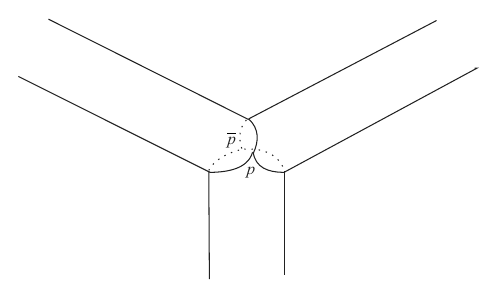
\includegraphics[width=.52\textwidth]{chapters/ch21-spectral-construction/figures/figure-21-1.png}
 \caption{一个极小面积度量。}
 \label{fig:21-minimal-area-metric}
\end{figure}

按如下方式把 $\Sigma$ 认作 $\Sigma_i$ 之并：
\[
 \Sigma=\bigcup_{i=1}^3\Sigma_i.
\]
若把 $\Sigma_i$ 等同于 $(-\infty,0]\times S^1$，则 $\Sigma$ 中存在三条从 $p$ 连接
到 $\bar p$、长度为 $1/2$ 的道路 $\theta_i$，$i=1,2,3$，使
\begin{equation}
 \begin{aligned}
 \partial_1\Sigma&=\theta_1\circ\theta_3^{-1},\\
 \partial_2\Sigma&=\theta_2\circ\theta_1^{-1},\\
 \partial_3\Sigma&=\theta_3\circ\theta_2^{-1}
 =(\theta_1\circ\theta_3^{-1})^{-1}\circ
 (\theta_2\circ\theta_1^{-1})^{-1}.
 \end{aligned}
 \label{eq:21-pants-gluing-rule}
\end{equation}
在这些坐标中，$p,\bar p$ 分别对应 $(s,t)=(0,0),(0,1/2)$。对 $i=1,2$ 固定
$\Sigma_i$ 与 $(-\infty,0]\times S^1$ 的全纯等同，其中
$S^1=\mathbb R/2\pi\mathbb Z$；并据分解~\eqref{eq:21-pants-gluing-rule} 把
$\Sigma_3$ 等同于 $[0,\infty)\times S^1$。记这些等同为
\[
 \varphi_i^-:\Sigma_i\to(-\infty,0]\times S^1,\quad i=1,2,
 \qquad
 \varphi_3^+:\Sigma_3\to[0,\infty)\times S^1,
\]
前者对应正穿孔，后者对应负穿孔；圆柱上的标准坐标记为 $(\tau,t)$。

现于三份 $[0,1]^2$ 上构造显式的哈密顿微分同胚二参数族。用
\eqref{eq:21-reparameterization-cutoff} 型函数对同痕的时间 $t$ 重参数化后，可设
$\phi_i$ 在 $t=0,1$ 附近关于时间为常值。公式为
\[
 \phi_1(s,t)=
 \begin{cases}
 \phi_{H_1}^{(1-s)t/(1-s/2)},&0\leq t\leq1-s/2,\\
 \phi_{H_1}^{1-s}\phi_{H_2}^{2(t-1+s/2)/s},&1-s/2\leq t\leq1,
 \end{cases}
\]
\[
 \phi_2(s,t)=
 \begin{cases}
 \phi_{H_1}^{2t},&0\leq t\leq s/2,\\
 \phi_{H_1}^{s}\phi_{H_2}^{(t-s/2)/(1-s/2)},&s/2\leq t\leq1,
 \end{cases}
\]
以及
\[
 \phi_3(s,t)=
 \begin{cases}
 \phi_{H_1}^{t(1+s)}\phi_{H_2}^{t(1-s)},&0\leq t\leq1-s/2,\\
 \phi_{H_1}^{(1+s)(1-s/2)}
 \phi_{H_2}^{2(t-1+s/2)/s},&1-s/2\leq t\leq1.
 \end{cases}
\]

\begin{exercise}
\label{ex:21-pants-family-compatibility}
核验该族与粘合规则~\eqref{eq:21-pants-gluing-rule} 的相容性，以及它在
$p,\bar p$ 之外的光滑性。
\end{exercise}

此外，从公式也可看出
\[
 \phi_1(0,t)=\phi_{H_1}^t,\qquad
 \phi_2(0,t)=\phi_{H_2}^t,\qquad
 \phi_3(1,t)=\phi_{H_1}^t\phi_{H_2}^t.
\]
相应联络在 $p,\bar p$ 外的平坦性，显然来自上述光滑的哈密顿微分同胚二参数族。

再用\termElongationFunction{}~$\rho$ 沿 $s$ 方向拉长裤子，得到 $\Sigma$ 上除 $p,\bar p$ 外处处光滑
的平坦联络。记平凡丛 $\dot\Sigma\times M\to\dot\Sigma$ 上的联络 1-形式为
\footnote{译者注：原文把联络 1-形式 $K$ 排成从 $\dot\Sigma$ 到
$\Omega^1(\dot\Sigma,C_0^\infty(M))$ 的映射，类型上似乎多出一层 $\dot\Sigma$；
译文照录。}
\[
 K:\dot\Sigma\longrightarrow\Omega^1(\dot\Sigma,C_0^\infty(M)).
\]
由于 $H_1,H_2$ 在边界附近平坦，它也在 $p,\bar p$ 处光滑，且曲率为 $0$。
\end{proof}

\begin{remark}
\label{rem:21-concatenation-hamiltonian}
同伦类 $[H_1\#H_2]$ 还可由拼接哈密顿量
\[
 H_1*H_2(t,x)=
 \begin{cases}
 2H_1(2t,x),&t\leq1/2,\\
 2H_2(2t-1,x),&t\geq1/2
 \end{cases}
\]
实现，而不必用 $H_1\#H_2$。这里假设 $H_1,H_2$ 在 $t=0,1$ 附近均边界平坦，
以保证相应联络光滑。这给出三元组 $(H_1,H_2;H_1*H_2)$ 所伴随的稍有不同的哈密顿
纤维化。不过 $H_1\#H_2$ 与 $H_1*H_2$ 同伦，故可把后者作为第三个哈密顿量
$H_3$；此时平坦联络的构造比使用 $H_1\#H_2$ 更明显。只须取
$\phi_3(s,t)\equiv\phi_3(0,t)$，并注意
\[
 \phi_3(0,t)=
 \begin{cases}
 \phi_{H_1}^{2t},&0\leq t\leq1/2,\\
 \phi_{H_1}^1\phi_{H_2}^{2t-1},&1/2\leq t\leq1,
 \end{cases}
\]
这正是道路 $\phi_{H_1}*\phi_{H_2}:t\mapsto\phi_{H_1*H_2}^t$。事实上，上述
$\phi_3$ 公式给出 $\phi_{H_1*H_2}$ 与 $\phi_{H_1}\phi_{H_2}$ 之间的显式同伦。
更多细节见 (FOOO11b)。
\end{remark}

现在证明三角不等式。令 $\alpha\in CF_*(H)$、$\beta\in CF_*(F)$ 是满足
$[\alpha]=a^\flat,[\beta]=b^\flat$ 的弗洛尔闭链，并令其裤子乘积闭链
$\alpha*\beta=:\gamma\in CF_*(H\#F)$。则
$[\alpha*\beta]=(a\cdot b)^\flat$，所以
\begin{equation}
 \rho(H\#F;a\cdot b)\leq\lambda_{H\#F}(\alpha*\beta).
 \label{eq:21-triangle-product-level}
\end{equation}
给定 $\delta>0$，选取 $\alpha,\beta$ 使
\begin{align}
 \lambda_H(\alpha)&\leq\rho(H;a)+\delta/2,
 \label{eq:21-alpha-near-minimax}\\
 \lambda_F(\beta)&\leq\rho(F;b)+\delta/2.
 \label{eq:21-beta-near-minimax}
\end{align}
于是可写
\[
 \alpha=\sum_i a_i[z_i,w_i],\quad
 \mathcal A_H([z_i,w_i])\leq\rho(H;a)+\delta/2,
\]
\[
 \beta=\sum_j a_j[z_j,w_j],\quad
 \mathcal A_F([z_j,w_j])\leq\rho(F;b)+\delta/2.
\]
下面用裤子乘积 (20.2.29) 估计 $\alpha*\beta\in CF_*(H\#F)$ 的层级。

回忆 (4.3.16) 与命题~\ref{prop:20-energy-curvature-identity} 中的恒等式
\[
 \int v^*\Omega_E=-\mathcal A_{H_1\#H_2}([z_3,w_3])
 +\mathcal A_{H_1}([z_1,w_1])+\mathcal A_{H_2}([z_2,w_2])
\]
及
\[
 E_{(K,J)}(u)=\int v^*\Omega_E+R_K(u),
\]
其中对任意 $u\in\mathcal M(K,J;\widetilde z)$，$v(z)=(z,u(z))$。
按 $*$ 的定义，对任意 $[z_3,w_3]\in\alpha*\beta$，存在
$[z_1,w_1]\in\alpha$、$[z_2,w_2]\in\beta$，使
$\mathcal M(K,J;\widetilde z)$ 在渐近条件
\[
 \widetilde z=([z_1,w_1],[z_2,w_2];[z_3,w_3])
\]
下非空。应用引理~\ref{lem:21-small-curvature-connection} 及
\eqref{eq:21-triangle-product-level}--\eqref{eq:21-beta-near-minimax}，立即得到
\begin{align}
 \mathcal A_{H\#F}([z_3,w_3])
 &\leq\mathcal A_H([z_1,w_1])+\mathcal A_F([z_2,w_2])+\delta\notag\\
 &\leq\lambda_H(\alpha)+\lambda_F(\beta)+\delta\notag\\
 &\leq\rho(H;a)+\rho(F;b)+2\delta
 \label{eq:21-triangle-action-estimate}
\end{align}
对所有 $[z_3,w_3]\in\alpha*\beta$ 成立。合并
\eqref{eq:21-triangle-product-level}--\eqref{eq:21-triangle-action-estimate}，有
\[
 \rho(H\#F;a\cdot b)\leq\rho(H;a)+\rho(F;b)+2\delta.
\]
令 $\delta\to0$，即得
\[
 \rho(H\#F;a\cdot b)\leq\rho(H;a)+\rho(F;b),
\]
三角不等式得证。

\section{谱性公理}
\label{sec:spectrality-axiom}

一般辛流形、特别是无理辛流形 $(M,\omega)$ 上的谱不变量 $\rho(H;a)$ 有如下最为
非平凡的性质之一：
\begin{equation}
 \text{（谱性）}\qquad \rho(H;a)\in\operatorname{Spec}(H)
 \label{eq:21-spectrality}
\end{equation}
对\emph{任意} $H$ 与 $a\in QH^*(M)$ 成立。对任意\emph{有理}辛流形，即使 $H$ 退化，这一性质
也相对容易证明；见 (Oh05c)。
\footnote{译者注：原文此处再次把谱性写成对所有 $a\in QH^*(M)$ 成立，但
定义~\ref{def:21-spectral-invariant} 只对 $a\neq0$ 定义实值谱不变量；译文照录。}

另一方面，对\emph{无理}辛流形迄今只证明了以下较弱版本；退化哈密顿量是否满足谱性仍是
未知的：
\stfhIndex{I136}{Feituihuapuxing}{非退化谱性（nondegenerate spectrality）}
\[
 \tag{非退化谱性}
 \text{对任意非退化 }H\text{ 及 }a\in QH^*(M),
 \quad\eqref{eq:21-spectrality}\text{ 成立。}
\]

\begin{question}
\label{prob:21-degenerate-irrational-spectrality}
无理辛流形上的退化哈密顿量是否满足谱性公理？若否，构造一个违反谱性公理的
哈密顿量。
\end{question}

不过，结合柔性逼近论证，这一非退化谱性足以证明一般的 $\rho(H;a)$ 同伦不变性；
\stfhIndex{I169}{JinFuluoerbilian}{紧弗洛尔闭链（tight Floer cycle）}
见 21.6 节。(Oh05c, Oh09a) 给出的谱性证明方案依赖\emph{紧弗洛尔闭链}的存在性。

\begin{definition}
\label{def:21-tight-floer-cycle}
若弗洛尔闭链 $\alpha\in CF(H)$ 满足：对任意与其同调的弗洛尔闭链
$\alpha'\in CF(H)$，即 $\alpha'-\alpha=\partial_{(H,J)}\gamma$，都有
\[
 \lambda_H(\alpha')\geq\lambda_H(\alpha),
\]
则称 $\alpha$ 是\emph{紧}的。
\end{definition}

本节尝试在起初不假设辛流形有理性的前提下证明谱性，解释这个几何论证在无理情形
下可能出错之处，再对任意哈密顿量——无论是否非退化——证明有理情形的谱性。
关于无理情形非退化谱性的完整证明，参见 (Oh09a) 或 (Ush08)。(Oh09a) 的证明是
几何的，并在称作\emph{瑟夫同伦}的通有单参数哈密顿量族下证明谱不变量的许多其他性质；
(Ush08) 的证明则是纯代数的，因为它适用于 13.8 节意义下的任意抽象弗洛尔复形。

\stfhIndex{I050}{Dianfanbozhumian}{典范薄柱面（canonical thin cylinder）}
回忆\termCanonicalThinCylinder{} (18.2.7) 的定义。重要的是，$u_{zz'}^{\mathrm{can}}$ 的像包含在
$z$（或 $z'$）的小邻域内；当 $z,z'$ 在 $C^1$ 拓扑中趋于环路 $z_\infty$ 时，它一致
收敛到 $z_\infty$。因此，在满足边界条件
\[
 u(0,t)=z(t),\qquad u(1,t)=z'(t)
\]
的映射 $u:[0,1]\times S^1\to M$ 的同伦类集合中，$u_{zz'}^{\mathrm{can}}$ 也选出
一个典范同伦类 $[u_{zz'}^{\mathrm{can}}]$。

\begin{lemma}
\label{lem:21-canonical-cylinder-area}
设 $z,z':S^1\to M$ 是两条光滑环路，$u^{\mathrm{can}}$ 是 (18.2.7) 给出的上述典范
圆柱。对 $z$ 的任意填充圆盘 $w$ 及附近环路 $z'$，关联 $z'$ 的填充圆盘
\[
 w':=w\#u_{zz'}^{\mathrm{can}}.
\]
当 $d_{C^1}(z,z')\to0$ 时，$u_{zz'}^{\mathrm{can}}$ 在 $C^1$ 拓扑中收敛，且其几何
面积 $\operatorname{Area}(u^{\mathrm{can}})$ 趋于零。特别地，当 $z'\to z$ 且
$d_{C^1}(z,z')\to0$ 时：
\footnote{译者注：原文只说 $u_{zz'}^{\mathrm{can}}$ 在 $C^1$ 拓扑中“收敛”，
却没有给出其极限；随后第 (1) 项明确陈述的是拼接圆盘 $w'\to w$。译文照录。}
\begin{enumerate}[label=(\arabic*)]
 \item 作为单位圆盘到 $M$ 的映射，$w'\to w$ 于 $C^1$ 拓扑；
 \item 辛面积满足
 \begin{equation}
  \int_{u_{zz'}^{\mathrm{can}}}\omega\longrightarrow0.
  \label{eq:21-thin-cylinder-symplectic-area}
 \end{equation}
\end{enumerate}
\end{lemma}

\begin{proof}
第 (1) 项立即来自上述\termCanonicalThinCylinder{}的显式形式及指数映射的标准性质。另一方面，由\termCanonicalThinCylinder{}的显式表达与指数映射的性质，容易作面积估计，得到当
$d_{C^1}(z,z')\to0$ 时 $\operatorname{Area}(u_{zz'}^{\mathrm{can}})\to0$。因
$z,z'$ 均为 $C^1$ 的，$u_{zz'}^{\mathrm{can}}$ 也是 $C^1$ 的，故
\[
 \operatorname{Area}(u_{zz'}^{\mathrm{can}})
 \geq\left|\int_{u_{zz'}^{\mathrm{can}}}\omega\right|.
\]
这蕴含当 $z'\to z$ 于 $C^1$ 拓扑时，
$\int_{u_{zz'}^{\mathrm{can}}}\omega\to0$。
\end{proof}

目标是证明极小极大值 $\rho(H;a)$ 是临界值，即存在
$[z,w]\in\widetilde{\mathcal L}_0(M)$ 使
\[
 \mathcal A_H([z,w])=\rho(H;a),\qquad
 d\mathcal A_H([z,w])=0,
 \quad\text{即}\quad \dot z=X_H(z).
\]
此前已证明 $\rho(H;a)$ 有限。

\begin{theorem}
\label{thm:21-rational-spectrality}
设 $(M,\omega)$ 有理，则任意哈密顿量 $H$ 均满足谱性公理，不要求 $H$ 非退化。
\end{theorem}

\begin{proof}
我们可以通过反证法证明：对于任意光滑哈密顿量，谱性公理成立，证明如下。
若 $H$ 非退化，就固定 $H$；否则在 $C^2$ 拓扑中以非退化哈密顿量序列
$H_i$ 逼近 $H$。选取弗洛尔闭链 $\alpha_i\in CF_*(H_i)$，使
$\lambda_{H_i}(\alpha_i)\to\rho(H;a)$。令
$\operatorname{peak}(\alpha_i)=[z_i,w_i]\in\operatorname{Crit}\mathcal A_{H_i}$。
则
\begin{equation}
 \lim_{i\to\infty}\mathcal A_{H_i}([z_i,w_i])=\rho(H;a).
 \label{eq:21-peak-action-limit}
\end{equation}
由 $\rho(\,\cdot\,;a)$ 的定义及有限性，可选出这样的序列。

现在我们证明序列 $[z_i,w_i]$ 在 $\widetilde{\mathcal L}_0(M)$ 上是预紧的。
因 $M$ 紧、$H_i\to H$ 于 $C^2$ 拓扑且 $\dot z_i=X_{H_i}(z_i)$，标准自举论证给出
$z_i$ 的一个子列（仍记 $z_i$）收敛到某环路 $z_\infty:S^1\to M$，且
$\dot z_\infty=X_H(z_\infty)$。由于固定了非零量子上同调类
$a\in QH^*(M)$（更具体地说，固定了它的次数），并且 $[\alpha_i]=a^\flat$，有
\[
 \mu_{H_i}([z_i,w_i])=\mu_{H_j}([z_j,w_j]).
\]

对充分大的 $i$，考虑 $z_\infty$ 的填充圆盘
\[
 w'_i=w_i\#u_{i\infty}^{\mathrm{can}},
\]
其中 $u_{i\infty}^{\mathrm{can}}=u_{z_i z_\infty}^{\mathrm{can}}$ 是 $z_i$ 与
$z_\infty$ 之间的\termCanonicalThinCylinder{}。其几何面积在 $i\to\infty$ 时趋于零。计算临界点
$[z_\infty,w'_i]\in\operatorname{Crit}\mathcal A_H$ 的作用量：
\begin{align}
 \mathcal A_H([z_\infty,w'_i])
 &=-\int_{w'_i}\omega-\int_0^1H(t,z_\infty(t))\,dt \notag\\
 &=-\int_{w_i}\omega-\int_{u_{i\infty}^{\mathrm{can}}}\omega
   -\int_0^1H(t,z_\infty(t))\,dt \notag\\
 &=\left(-\int_{w_i}\omega-\int_0^1H_i(t,z_i(t))\,dt\right)
   -\int_{u_{i\infty}^{\mathrm{can}}}\omega \notag\\
 &\quad-\left(\int_0^1H(t,z_\infty(t))\,dt
   -\int_0^1H_i(t,z_i(t))\,dt\right) \notag\\
 &=\mathcal A_{H_i}([z_i,w_i])
   -\int_{u_{i\infty}^{\mathrm{can}}}\omega \notag\\
 &\quad-\left(\int_0^1H(t,z_\infty(t))\,dt
   -\int_0^1H_i(t,z_i(t))\,dt\right).
 \label{eq:21-limit-action-computation}
\end{align}
由于 $z_i$ 一致收敛到 $z_\infty$ 且 $H_i\to H$，
\begin{equation}
 -\left(\int_0^1H(t,z_\infty(t))dt
 -\int_0^1H_i(t,z_i(t))dt\right)\longrightarrow0.
 \label{eq:21-hamiltonian-integral-limit}
\end{equation}
结合~\eqref{eq:21-peak-action-limit}--\eqref{eq:21-hamiltonian-integral-limit}，得到
\[
 \lim_{i\to\infty}\mathcal A_H([z_\infty,w'_i])=\rho(H;a).
\]
故 $\mathcal A_H([z_\infty,w'_i])$ 是柯西序列，从而
\[
 \left|\int_{w'_i}\omega-\int_{w'_j}\omega\right|
 =|\mathcal A_H([z_\infty,w'_i])-\mathcal A_H([z_\infty,w'_j])|
 \longrightarrow0,
\]
即
\[
 \int_{w'_i\#\overline{w'_j}}\omega\longrightarrow0.
\]
因 $\Gamma$ 离散且 $[w'_i\#\overline{w'_j}]_\omega\in\Gamma$，对充分大的
$i,j\in\mathbb Z_+$，必有
\begin{equation}
 \int_{w'_i\#\overline{w'_j}}\omega=0.
 \label{eq:21-rational-area-stabilization}
\end{equation}
特别地，数集 $\{\int_{w'_i}\omega\}_{i\in\mathbb Z_+}$ 有界；必要时取子列，可认为
序列 $\int_{w'_i}\omega$ 最终稳定。由 $\mathcal A_H$ 的定义，对任意充分大的 $N$，
$\mathcal A_H([z_\infty,w'_N])=
\lim_{i\to\infty}\mathcal A_H([z_\infty,w'_i])$。回到
\eqref{eq:21-limit-action-computation} 可见作用量本身稳定，故
\[
 \mathcal A_H([z_\infty,w'_N])
 =\lim_{i\to\infty}\mathcal A_H([z_\infty,w'_i])=\rho(H;a).
\]
所以 $\rho(H;a)$ 确为 $\mathcal A_H$ 在临界点 $[z_\infty,w'_N]$ 处的值。
这就是对无理情形不成立的关键所在。
\end{proof}

上述有理情形证明中，下述引理起关键作用。部分由于它在无理情形下失效，即使只论
非退化情形，无理情形谱性的证明也远比有理情形非平凡。

\begin{lemma}
\label{lem:21-rational-critical-set-compactness}
当 $(M,\omega)$ 有理时，对任意光滑哈密顿量 $K$，
$\operatorname{Crit}\mathcal A_K\subset\widetilde{\mathcal L}_0(M)$ 是
$\mathbb R$ 的闭子集，并且在覆盖空间
$\pi:\widetilde{\mathcal L}_0(M)\to\mathcal L_0(M)$ 的子空间拓扑中局部紧。
\footnote{译者注：原文称
$\operatorname{Crit}\mathcal A_K\subset\widetilde{\mathcal L}_0(M)$ 是
“$\mathbb R$ 的闭子集”，但证明只说明它在覆盖空间中闭；译文照录该类型疑点。}
\end{lemma}

\begin{proof}
当 $(M,\omega)$ 有理时，上述 $\pi$ 的覆盖群 $\Gamma$ 离散。再结合紧流形 $M$ 上
方程 $\dot z=X_K(z)$ 的解集紧，可知
\[
 \operatorname{Crit}(\mathcal A_K)
 =\{[z,w]\in\widetilde{\mathcal L}_0(M)\mid\dot z=X_K(z)\}
\]
是闭集且局部紧。
\end{proof}

无理情形非退化谱性的证明最早由 (Oh09a) 给出（半正情形）。该证明使用连续性方法，
从一个小莫尔斯函数出发沿\emph{瑟夫同伦}推进，并细致分析与谱不变量对应的临界值如何
\stfhIndex{I190}{Eshe}{厄舍（Usher）}
变化。后来厄舍 (Ush08) 基于非阿基米德分析中一条优美的逼近定理，在 13.8 节所述
弗洛尔同调公理框架中给出简洁的代数证明。这里只陈述厄舍的第 13.8 节框架下
非退化谱性公理的抽象表述；其证明
依赖紧闭链的存在性，细节见 (Ush08)。回忆定义 13.8.1 中的
$\operatorname{Spec}(\mathfrak c)$。

\begin{theorem}[定理 1.4 (Ush08)]
\label{thm:21-usher-spectrality}
设 $\mathfrak c$ 是诺特环 $R$ 上的滤过弗洛尔--诺维科夫复形。则对每个
$a\in H_*(\mathfrak c)$，存在 $\alpha\in C_*(\mathfrak c)$ 使
$[\alpha]=a$ 且 $\rho(a)=\lambda(\alpha)$。特别地，
$\rho(a)\in\operatorname{Spec}(\mathfrak c)$。
\end{theorem}

对任意非退化哈密顿量 $H$ 的弗洛尔复形
$(CF_*(H),\partial_{(H,J)})$，此定理说明谱数 $\rho(H;a)$ 由一条紧弗洛尔闭链
$\alpha$ 的层级实现，即 $\lambda_H(\alpha)=\rho(H;a)$。特别地，
$\rho(H;a)\in\operatorname{Spec}(H)$，这就证明了 $\rho(H;a)$ 的非退化谱性。

\section{同伦不变性}
\label{sec:spectral-homotopy-invariance}

下述命题说明函数 $\rho_a=\rho(\,\cdot\,;a)$ 下降为
$\widetilde{\operatorname{Ham}}(M,\omega)$ 上的连续函数。

\begin{theorem}[同伦不变性]
\label{thm:21-spectral-homotopy-invariance}
设 $(M,\omega)$ 是任意闭辛流形，并假设 $(M,\omega)$ 满足非退化谱性公理。则对任意
光滑函数 $H\sim K$，即满足 $\phi_H^1=\phi_K^1$ 且 $\phi_H,\phi_K$ 相对于端点道路
同伦的函数，都有
\begin{equation}
 \rho(\underline H;a)=\rho(\underline K;a).
 \label{eq:21-spectral-homotopy-equality}
\end{equation}
\end{theorem}

本节将给出该定理的两个不同证明，每一个都包含弗洛尔理论研究中的若干重要成分。
暂且推迟证明，先陈述其推论。由同伦不变性，可对代表
$h=[\phi_H]$ 的任意 $H$（无论 $h$ 是否非退化）定义
\begin{equation}
 \rho_a(h):=\rho(H;a).
 \label{eq:21-spectral-function-cover}
\end{equation}
这给出良定义函数
\[
 \rho_a:\widetilde{\operatorname{Ham}}(M,\omega)\longrightarrow\mathbb R.
\]

\begin{theorem}
\label{thm:21-spectral-function-continuous-cover}
在由 $P^{\mathrm{ham}}(\operatorname{Symp}(M,\omega),\mathrm{id})$ 诱导的商拓扑下，
$\rho_a$ 是 $\widetilde{\operatorname{Ham}}(M,\omega)$ 上的连续函数。
\end{theorem}

\begin{proof}
回忆商映射
\[
 \pi:P^{\mathrm{ham}}(\operatorname{Symp}(M,\omega),\mathrm{id})
 \longrightarrow\widetilde{\operatorname{Ham}}(M,\omega).
\]
已经证明赋值
\begin{equation}
 \lambda\longmapsto\rho(\lambda;a)
 \label{eq:21-spectral-function-path-space}
\end{equation}
在道路空间上连续。按商拓扑定义，
$\rho_a:\widetilde{\operatorname{Ham}}(M,\omega)\to\mathbb R$ 连续，因为复合
\[
 \rho_a\circ\pi:
 P^{\mathrm{ham}}(\operatorname{Symp}(M,\omega),\mathrm{id})\longrightarrow\mathbb R
\]
正是~\eqref{eq:21-spectral-function-path-space}。
\end{proof}

\subsection{使用非退化谱性的证明}

先考虑满足 $H\sim K$ 的非退化哈密顿量。回忆以下基本事实：
\begin{enumerate}[label=(\arabic*)]
 \item 哈密顿函数 $H$ 的非退化性只依赖其时间一映射 $\phi=\phi_H^1$；
 \item $\operatorname{Spec}(H)\subset\mathbb R$，即作用量泛函 $\mathcal A_H$ 的
 临界值集，是零测集（见 (Oh02) 的引理 2.2）；
 \item 若 $H,H'\mapsto\phi$ 且 $H\sim H'$，并且二者已归一化，则
 $\operatorname{Spec}(H)=\operatorname{Spec}(H')$（命题 18.3.6）；
 \item 函数 $H\mapsto\rho(H;a)$ 关于 $C_0^\infty(S^1\times M)$ 上的光滑拓扑连续
 （命题~\ref{prop:21-spectral-continuity}）；
 \item 从连通空间（例如区间 $[0,1]$）到 $\mathbb R$ 且值落在某个零测子集中的连续
 函数，只能是常函数。
\end{enumerate}

因 $H\sim K$，存在光滑族 $\mathcal H=\{H(s)\}_{0\leq s\leq1}$，使
$H(0)=H,H(1)=K$。定义 $\rho:[0,1]\to\mathbb R$ 为
$\rho(s)=\rho(H(s);a)$。由于所有 $s$ 的时间一映射均为
$\phi_{H(s)}^1=\phi_H^1$，$H(s)$ 都非退化；其像落在与 $s$ 无关的\emph{固定}子集
$\operatorname{Spec}(h)\subset\mathbb R$ 中，其中 $h=[H]=[K]$ 是道路同伦类。
由上述第 (2) 项，该集为零测集，因而全不连通。函数 $\rho$ 又由 $C^0$-连续性公理
连续，故必为常函数，于是
$\rho(H;a)=\rho(0)=\rho(1)=\rho(K;a)$，证明了非退化情形。
\footnote{译者注：原文此处回指第 (1) 项，但“作用谱是零测集”是上列第 (2) 项；
译文改正编号。}
\footnote{译者注：这里 $\rho$ 已被定义为参数函数 $s\mapsto\rho(H(s);a)$；原文等式
同时写 $\rho(H;a)$ 与 $\rho(0)$，记号层次混用，译文照录。}

现设 $H$ 退化。要强调的是，目前尚不知道退化哈密顿量是否满足谱性公理，因此不能
把上述非退化证明方案直接用于退化情形。改用基于下述引理的逼近论证。

\begin{lemma}
\label{lem:21-common-morse-perturbation}
设未必非退化的 $H\sim K$。则存在 $C^2$-收敛到 $0$ 的莫尔斯函数序列 $f_i$，使
$H\#f_i\sim K\#f_i$，且 $H\#f_i,K\#f_i$ 均非退化。
\end{lemma}

\begin{proof}
留作习题。
\end{proof}

应用此引理，
\[
 \rho(H;a)=\lim_{i\to\infty}\rho(H\#f_i;a)
 =\lim_{i\to\infty}\rho(K\#f_i;a)=\rho(K;a).
\]
第一种证明完成。

\stfhIndex{I147}{Zuiyouyantuo}{最优延拓（optimal continuation）}
\subsection{使用最优延拓的证明}

回忆同伦不变性的设定。给定 $H_0,H_1$，满足
$\phi_{H_0}^1=\phi_{H_1}^1$ 且 $[H_0]=[H_1]$。按定义，存在二参数族
$\{\phi(s,t)\}\subset\operatorname{Ham}(M,\omega)$，$(s,t)\in[0,1]^2$。存在
$\psi\in\operatorname{Ham}(M,\omega)$，使
\begin{equation}
 \begin{aligned}
 \phi(s,0)&\equiv\mathrm{id},&\quad \phi(s,1)&\equiv\psi
 &&\text{对所有 }s\in[0,1],\\
 \phi(0,t)&=\phi_{H_0}^t,& \phi(1,t)&=\phi_{H_1}^t
 &&\text{对所有 }t\in[0,1].
 \end{aligned}
 \label{eq:21-two-parameter-isotopy-boundary}
\end{equation}
记 $\mathcal H=H(s,t,x)$，其中 $H^s=H(s,\,\cdot\,,\,\cdot\,)$ 是生成向量场
\[
 \frac{\partial\phi}{\partial t}\circ\phi^{-1}
\]
的哈密顿量；又以 $F=F(s,t,x)$ 表示生成相应 $s$-哈密顿向量场
\[
 \frac{\partial\phi}{\partial s}\circ\phi^{-1}
\]
的哈密顿量。由~\eqref{eq:21-two-parameter-isotopy-boundary}，在 $t=0,1$ 附近沿
$t$ 方向、在 $s=0,1$ 附近沿 $s$ 方向重参数化
$\phi:[0,1]^2\to\operatorname{Ham}(M,\omega)$ 后，可设
\[
 F\equiv0\quad\text{于}\quad
 ([0,\epsilon]\times[0,1])\cup([1-\epsilon,1]\times[0,1]),
\]
特别地，$s$-哈密顿向量场 $X_F$ 对每个 $s$ 都关于 $t$ 一周期。

对给定 $[z^-,w^-]$、$[z^+,w^+]$，且
$[w^-\#u]=[w^+]\in\pi_2(z^+)$，考虑扰动柯西--黎曼方程
\begin{equation}
 \begin{cases}
 \partial u/\partial\tau-X_{F^\rho}(u)
 +J(\partial u/\partial t-X_{H^\rho}(u))=0,\\
 u(-\infty)=z^-,\quad u(\infty)=z^+,
 \end{cases}
 \label{eq:21-optimal-continuation-equation}
\end{equation}
并寻找有限能量解，其中
\[
 E_{(\phi^\rho,J)}(u):=\frac12\int_{\mathbb R\times[0,1]}
 \left(
 \left\lVert\frac{\partial u}{\partial\tau}-X_{F^\rho}(u)\right\rVert_J^2
 +\left\lVert\frac{\partial u}{\partial t}-X_{H^\rho}(u)\right\rVert_J^2
 \right).
\]
此方程等价于 $(du+P_{(K,J)}(u))^{0,1}=0$，其中
$K=H^\rho dt+F^\rho d\tau$。由于 $(H,F)$ 来自二参数族 $\phi$，有 $R_K\equiv0$。
又因 $F$ 在 $s=0,1$ 附近为 $0$，对充分大的 $R>0$，当 $|\tau|>R$ 时
$F^\rho\equiv0$。特别地，$\tau<-R$ 时~\eqref{eq:21-optimal-continuation-equation}
成为
\[
 \frac{\partial u}{\partial\tau}
 +J\left(\frac{\partial u}{\partial t}-X_{H_0}(u)\right)=0,
\]
而 $\tau>R$ 时成为
\[
 \frac{\partial u}{\partial\tau}
 +J\left(\frac{\partial u}{\partial t}-X_{H_1}(u)\right)=0.
\]

考察零维模空间以定义映射
\[
 h_{(\phi^\rho,J)}:CF(H_0,J_0)\longrightarrow CF(H_1,J_1),
\]
再如前考察一维模空间以证明它是链映射。还要分析该链映射如何影响弗洛尔复形的
滤过；为此，\emph{当}~\eqref{eq:21-optimal-continuation-equation} 有\emph{有限}能量解时，需研究
作用量差
\[
 \mathcal A_{H_0}([z^-,w^-])-
 \mathcal A_{H_1}([z^+,w^-\#u]).
\]
先回忆基本恒等式
\begin{equation}
 R_K=\frac{\partial F^\rho}{\partial t}
 -\frac{\partial H^\rho}{\partial\tau}
 +\{F^\rho,H^\rho\}=0.
 \label{eq:21-flat-curvature-identity}
\end{equation}
这是因为对子 $(H^\rho,F^\rho)$ 来自二参数同痕
$\phi=\phi(s,t)\in\operatorname{Ham}(M,\omega)$。对
\eqref{eq:21-optimal-continuation-equation} 应用命题
\ref{prop:20-energy-curvature-identity}，并用 $R_K=0$，得到
\[
 \mathcal A_{H_1}([z^+,w^-\#u])-\mathcal A_{H_0}([z^-,w^-])
 =-E_{(\phi^\rho,J)}(u)\leq0.
\]

\begin{proposition}
\label{prop:21-optimal-continuation-action}
设 $\phi=\{\phi(s,t)\}$ 及其相应对子 $(H,F)$ 如上。令
$\rho:\mathbb R\to[0,1]$ 光滑，且对某个 $R>0$，在 $\tau\leq-R$ 时
$\rho\equiv0$，在 $\tau\geq R$ 时 $\rho\equiv1$。给定
$[z^-,w^-]\in\operatorname{Crit}\mathcal A_{H_0}$，设
$u:\mathbb R\times[0,1]\to M$ 是~\eqref{eq:21-optimal-continuation-equation} 的解，
满足 $u(-\infty)=z^-,u(\infty)=z^+$。则
\begin{equation}
 \mathcal A_{H_1}([z^+,w^-\#u])
 \leq\mathcal A_{H_0}([z^-,w^-]).
 \label{eq:21-optimal-continuation-action-bound}
\end{equation}
\end{proposition}

立即得到：

\begin{corollary}
\label{cor:21-optimal-continuation-filtration}
链映射 $h_{(\phi;J)}:CF(H_0,J_0)\to CF(H_1,J_1)$ 保持滤过，即对所有
$\lambda\in\mathbb R$ 诱导链映射
\[
 h_{(\phi;J)}^\lambda:CF^\lambda(H_0,J_0)
 \longrightarrow CF^\lambda(H_1,J_1).
\]
\end{corollary}

显然，$s$-时间反演同痕
\[
 \widetilde\phi(s,t):=\phi(1-s,t)
\]
诱导保滤过映射
$h_{(\widetilde\phi;\widetilde J)}:
CF^\lambda(H_1,J_1)\to CF^\lambda(H_0,J_0)$。

现在完成 $\rho(H_0;a)=\rho(H_1;a)$ 的证明。只须证
$\rho(H_0;a)\leq\rho(H_1;a)$，反向同理，只需考虑 $s$-时间反演。给定
$\epsilon>0$，存在弗洛尔链 $\alpha_{H_1}$，使
$[\alpha_{H_1}]=a^\flat$ 且
$\lambda_{H_1}(\alpha_{H_1})\leq\rho(H_1;a)+\epsilon$。于是
\[
 \lambda_{H_0}\bigl(h_{(\widetilde\phi;\widetilde J)}(\alpha_{H_1})\bigr)
 \leq\lambda_{H_1}(\alpha_{H_1})\leq\rho(H_1;a)+\epsilon.
\]
又因 $h_{(\widetilde\phi;\widetilde J)}(\alpha_{H_1})\in CF_*(H_0)$ 且其同调类为
$a^\flat$，
\[
 \rho(H_0;a)
 \leq\lambda_{H_0}\bigl(h_{(\widetilde\phi;\widetilde J)}(\alpha_{H_1})\bigr)
 \leq\rho(H_1;a)+\epsilon.
\]
令 $\epsilon\to0$ 即得 $\rho(H_0;a)\leq\rho(H_1;a)$。这证明了哈密顿微分同胚
$\psi=\phi_{H_0}^1=\phi_{H_1}^1$ 非退化时的结论。一般情形由
$H\mapsto\rho(H;a)$ 的 $C^0$-连续性推出。


\chapter{谱不变量：应用}
\label{ch:spectral-applications}

尽管谱不变量的构造严重依赖伪全纯曲线的解析理论，尤其依赖辛流形的光滑结构，
但这些不变量本身却是 $C^0$ 型不变量：它们在 (OhM07) 所引入的 $C^0$-哈密顿拓扑
（亦见本书第 6.2 节）中连续，因而可以延拓到第 6.2 节所定义的拓扑哈密顿流。

本章说明谱不变量在辛拓扑研究中的若干应用。与霍费尔型的其他更直接的动力学不变量
相比，谱不变量的一项重要优势是其\emph{同伦不变性}；这使我们能够自然地把谱不变量推前到
哈密顿微分同胚群的万有覆盖空间，有时甚至还能降到群本身。恩托夫与波尔捷罗维奇
(EnP06) 对部分辛拟态的惊人构造突出体现了这一点：该构造只以谱不变量
$\rho(H;1)$ 的公理性质以及动力系统中取渐近平均这一自然运算为基础。他们在单调情形
下完成了这一构造，随后厄舍 (Ush10b) 将之推广到任意紧辛流形。

首先，我们将说明 (Oh05d) 中不变谱范数的构造，以及它在辛刚性问题和霍费尔几何中
测地线极小性问题上的应用。我们还将说明厄舍对波尔捷罗维奇以及拉隆德--麦克达夫
极小性猜想和最优能量--容量不等式的应用。其次，我们将自足地介绍恩托夫与
波尔捷罗维奇从谱不变量构造的部分辛拟态与拟同态，以及它们在辛相交问题中的应用。
最后，我们回到哈密顿同胚群的研究，并说明如何把所有这些构造延拓到第 6 章意义下的
连续哈密顿范畴。

看来，这些构造作为一个整体对辛拓扑的发展颇为重要；从纯辛拓扑的观点看，这一发展
正开始揭示格罗莫夫伪全纯曲线与弗洛尔同调之真正含义所笼罩的神秘面纱。

\section{哈密顿微分同胚的谱范数}
\label{sec:spectral-norm-hamiltonian-diffeomorphisms}

本节依照 (Oh05d) 说明哈密顿微分同胚的一种不变范数的构造；它称为\emph{谱范数}。
这里需要谨慎使用对应于量子上同调类 $1\in QH^*(M)$ 的谱不变量 $\rho(H;1)$。

回忆 $C^\infty([0,1]\times M)$ 上有自然对合
\[
 H\longmapsto\overline H;\qquad
 \overline H(t,x)=-H(t,\phi_H^t(x)),
\]
它也等价于取逆的对合
\[
 \lambda\longmapsto\lambda^{-1};\qquad
 \mathcal P^{\mathrm{ham}}(\operatorname{Symp}(M,\omega),\mathrm{id})
 \longrightarrow
 \mathcal P^{\mathrm{ham}}(\operatorname{Symp}(M,\omega),\mathrm{id}).
\]
我们关于这个对合将 $\rho(\mathord\cdot;1)$ 对称化，并定义函数
\[
 \gamma:C^\infty([0,1]\times M)\longrightarrow\mathbb R
\]
为
\begin{equation}
 \gamma(H)=\rho(H;1)+\rho(\overline H;1)
 \label{eq:22-gamma-hamiltonian}
\end{equation}
（定义域为 $C^\infty([0,1]\times M)$）。显然，对任意 $H$ 都有
$\gamma(H)=\gamma(\overline H)$。一般三角不等式
\[
 \rho(H;a)+\rho(F;b)\geq\rho(H\#F;a\cdot b)
\]
限制到 $a=b=1$，再结合定理 21.3.7 的归一化公理 $\rho(\mathrm{id};1)=0$，便给出
\begin{equation}
 \gamma(H)=\rho(H;1)+\rho(\overline H;1)\geq\rho(0;1)=0.
 \label{eq:22-gamma-nonnegative}
\end{equation}
这里 $a\cdot b$ 是量子上同调类 $a,b\in QH^*(M)$ 的量子乘积，$0$ 是零函数。

下面把 $\gamma(H)$ 与 $L^{(1,\infty)}$-范数
$\lVert H\rVert=\int_0^1\operatorname{osc}(H_t)\,dt$ 比较。回忆定义
\begin{equation}
 E^-(H)=\int_0^1-\min H\,dt,
 \qquad
 E^+(H)=\int_0^1\max H\,dt,
 \label{eq:22-hofer-lengths}
\end{equation}
\stfhSubIndex{I109}{Huofeierchangdu}{霍费尔长度（Hofer length）}{Fu}{负霍费尔长度（negative Hofer length）}
\stfhSubIndex{I110}{Huofeierchangdu}{霍费尔长度（Hofer length）}{Zheng}{正霍费尔长度（positive Hofer length）}
分别称为负霍费尔长度与正霍费尔长度。显然
$E^+(\overline H)=E^-(H)$。我们证明下面的引理。

\begin{lemma}
\label{lem:22-spectral-hofer-bounds}
对任意 $H$ 和 $0\neq a\in QH^*(M)$，有
\begin{equation}
 -E^+(H)+v(a)\leq\rho(H;a)\leq E^-(H)+v(a),
 \label{eq:22-spectral-valuation-bounds}
\end{equation}
其中 $v(a)$ 是 $a$ 的\termValuation{}。特别地，对任意经典上同调类
$b\in H^*(M)\hookrightarrow QH^*(M)$，任意哈密顿量 $H$ 都满足
\begin{equation}
 -E^+(H)\leq\rho(H;b)\leq E^-(H).
 \label{eq:22-classical-hofer-bounds}
\end{equation}
\end{lemma}

\begin{proof}
从不等式 (21.3.22) 出发，即
\[
 \int_0^1-\max(H-K)\,dt
 \leq\rho(H;a)-\rho(K;a)
 \leq\int_0^1-\min(H-K)\,dt.
\]
可将它改写成
\[
 \rho(K;a)+\int_0^1-\max(H-K)\,dt
 \leq\rho(H;a)\leq
 \rho(K;a)+\int_0^1-\min(H-K)\,dt.
\]
令 $K\to0$，得到
\begin{equation}
 \rho(0;a)+\int_0^1-\max H\,dt
 \leq\rho(H;a)\leq
 \rho(0;a)+\int_0^1-\min H\,dt.
 \label{eq:22-zero-hamiltonian-bound}
\end{equation}
由归一化公理，$\rho(0;a)=v(a)$，故 (21.3.22) 变为
\[
 v(a)-E^+(H)\leq\rho(H;a)\leq v(a)+E^-(H).
\]
经典上同调类 $b$ 满足 $v(b)=0$，于是由定义立刻得到
\eqref{eq:22-classical-hofer-bounds}。
\end{proof}

把~\eqref{eq:22-classical-hofer-bounds} 的右侧分别用于 $b=1$ 和
$H,\overline H$，便有 $\rho(H;1)\leq E^-(H)$ 以及
$\rho(\overline H;1)\leq E^-(\overline H)$。另一方面，对任意 $H$，
$E^-(\overline H)=E^+(H)$，所以
\begin{equation}
 \gamma(H)\leq\lVert H\rVert.
 \label{eq:22-gamma-hofer-bound}
\end{equation}
非负性~\eqref{eq:22-gamma-nonnegative} 引出如下定义。

\begin{definition}
\label{def:22-spectral-norm}
定义 $\gamma:\operatorname{Ham}(M,\omega)\to\mathbb R_+$ 为
\[
 \gamma(\phi):=\inf_{H\mapsto\phi}\gamma(H)
 =\inf_{H\mapsto\phi}\bigl(\rho(H;1)+\rho(\overline H;1)\bigr).
\]
\stfhIndex{I175}{Pufanshu}{谱范数（spectral norm）}
称 $\gamma(\phi)$ 为 $\phi$ 的\emph{谱范数}。
\end{definition}

下面的定理概括函数 $\gamma$ 的基本性质。在本小节余下部分，我们将证明这些陈述；
其中最非平凡的非退化性留到下一小节。

\begin{theorem}
\label{thm:22-spectral-norm-properties}
设 $\gamma$ 如上。则
$\gamma:\operatorname{Ham}(M,\omega)\to\mathbb R_+$ 定义一个不变范数，即它满足：
\begin{enumerate}
 \item （非退化性）$\phi=\mathrm{id}$ 当且仅当 $\gamma(\phi)=0$；
 \item （辛不变性）对任意辛微分同胚 $\eta$，
 $\gamma(\eta^{-1}\phi\eta)=\gamma(\phi)$；
 \item （三角不等式）$\gamma(\phi\psi)\leq\gamma(\phi)+\gamma(\psi)$；
 \item （取逆不变性）$\gamma(\phi^{-1})=\gamma(\phi)$；
 \item $\gamma(\phi)\leq\lVert\phi\rVert$。
\end{enumerate}
\end{theorem}

\begin{proof}[辛不变性的证明]
回忆谱不变量的辛不变性
$\rho(H;a)=\rho(\eta_*H;\eta_*a)$。把它用于 $a=1$，并利用
$\eta_*1=1$，得到
\[
 \begin{aligned}
 \gamma(\phi)
 &=\inf_{H\mapsto\phi}\bigl(\rho(H;1)+\rho(\overline H;1)\bigr)\\
 &=\inf_{H\mapsto\phi}
 \bigl(\rho(\eta_*H;1)+\rho(\overline{\eta_*H};1)\bigr)
 =\gamma(\eta^{-1}\phi\eta).
 \end{aligned}
\]
\end{proof}

\begin{proof}[三角不等式的证明]
先回忆三角不等式
\begin{equation}
 \rho(H\#K;1)\leq\rho(H;1)+\rho(K;1)
 \label{eq:22-triangle-forward}
\end{equation}
以及
\begin{equation}
 \rho(\overline K\#\overline H;1)
 \leq\rho(\overline K;1)+\rho(\overline H;1).
 \label{eq:22-triangle-inverse}
\end{equation}
将~\eqref{eq:22-triangle-forward} 与~\eqref{eq:22-triangle-inverse} 相加，得到
\begin{align}
 \rho(H\#K;1)+\rho(\overline{H\#K};1)
 &=\rho(H\#K;1)+\rho(\overline K\#\overline H;1)\notag\\
 &\leq\bigl(\rho(H;1)+\rho(\overline H;1)\bigr)
 +\bigl(\rho(K;1)+\rho(\overline K;1)\bigr).
 \label{eq:22-gamma-triangle-hamiltonians}
\end{align}
现令 $H\mapsto\phi$、$K\mapsto\psi$。因为 $H\#K$ 生成 $\phi\psi$，所以
\[
 \gamma(\phi\psi)\leq\gamma(H\#K)
 =\rho(H\#K;1)+\rho(\overline{H\#K};1),
\]
进而由~\eqref{eq:22-gamma-triangle-hamiltonians} 得
\[
 \gamma(\phi\psi)\leq
 \bigl(\rho(H;1)+\rho(\overline H;1)\bigr)
 +\bigl(\rho(K;1)+\rho(\overline K;1)\bigr).
\]
让右端对所有 $H\mapsto\phi$ 与 $K\mapsto\psi$ 取下确界，即证性质 (3)。
\end{proof}

\begin{proof}[取逆不变性的证明]
由 $\gamma$ 的定义关于映射 $\phi\mapsto\phi^{-1}$ 对称，结论立即成立。
\end{proof}

\begin{proof}[性质 (5) 的证明]
令~\eqref{eq:22-gamma-hofer-bound} 对 $H\mapsto\phi$ 取下确界，便得
$\gamma(\phi)\leq\lVert\phi\rVert$。
\end{proof}

现在只剩证明 $\gamma$ 的非退化性。(Oh05d) 中的原证明使用了特定伪全纯曲线的一条
相当精细的存在性定理。尽管这条存在性定理本身对刚性问题有重要应用，我们仍将把非退化性
作为一个更熟悉的能量--容量型不等式的推论来给出另一证明；这个证明由厄舍 (Ush10a)
提出。它较为间接，需要暂时转向研究 $\operatorname{Ham}(M,\omega)$ 上的霍费尔几何。
（麦克达夫与萨拉蒙在 (MSa04) 中还给出了另一证明。）

\begin{remark}
\label{rem:22-medium-hofer-norm}
事实上，如果把 $\rho(\mathord\cdot;1)$ 的同伦不变性纳入
$\gamma(\phi)\leq\lVert\phi\rVert$ 的证明，就可以如下改进该不等式。定义\emph{中等霍费尔}
范数
\[
 \lVert\phi\rVert_{\mathrm{med}}
 :=\inf\{\lVert h\rVert\mid\pi(h)=\phi\},
\]
其中对 $h\in\widetilde{\operatorname{Ham}}(M,\omega)$ 定义
\[
 \lVert h\rVert:=\inf\{\lVert H\rVert
 \mid h=[\phi_H]\in\widetilde{\operatorname{Ham}}(M,\omega)\}.
\]
于是上述证明给出 $\gamma(H)\leq\lVert[\phi_H]\rVert$，从而
\[
 \gamma(\phi)\leq\lVert\phi\rVert_{\mathrm{med}}.
\]
更多相关讨论见 (Oh09a) 第 11 节。
\end{remark}

\stfhIndex{I129}{Zhongdenghuofeierfanshu}{中等霍费尔范数（medium Hofer norm）}
\section{霍费尔测地线与周期轨道}
\label{sec:hofer-geodesics-periodic-orbits}

本节研究哈密顿路径在霍费尔距离下的长度极小性。我们先沿用\personBialy{}与\personPolterovich{}
(BP94) 以及拉隆德与麦克达夫 (LM95b) 的做法，引入一个必要判据，再介绍厄舍 (Ush10a)
对所谓极小性猜想的证明。同时，我们也将依照厄舍的论证证明
$\operatorname{Ham}(M,\omega)$ 上 $\gamma$-范数的非退化性。

\subsection{准自治哈密顿量}

$H$ 的 $L^{(1,\infty)}$-范数
$\lVert H\rVert=\int_0^1(\max H_t-\min H_t)\,dt$ 可等同于路径
$\phi_H:t\mapsto\phi_H^t$ 的芬斯勒长度
\[
 \operatorname{leng}(\phi_H)=\int_0^1
 \bigl(\max_xH(t,\phi_H^t(x))-\min_xH(t,\phi_H^t(x))\bigr)\,dt,
\]
其中
\[
 T_{\mathrm{id}}\operatorname{Ham}(M,\omega)
 \cong C^\infty(M)/\mathbb R
\]
上的相伴巴拿赫范数正是
\[
 \lVert h\rVert=\operatorname{osc}(h)=\max h-\min h.
\]
映射 $t\mapsto H(t,\phi_H^t(\mathord\cdot))$ 可视为
$\operatorname{Ham}(M,\omega)$ 上路径 $t\mapsto\phi_H^t$ 的切向量。

\begin{definition}
\label{def:22-hofer-path-metric}
考虑定义在
$\mathcal P^{\mathrm{ham}}(\operatorname{Symp}(M,\omega),\mathrm{id})$ 上的度量
$d:\mathcal P^{\mathrm{ham}}(\operatorname{Symp}(M,\omega),\mathrm{id})
\to\mathbb R_+$：
\[
 d(\lambda,\mu):=\operatorname{leng}(\lambda^{-1}\circ\mu),
\]
其中 $\lambda^{-1}\circ\mu$ 是哈密顿路径
$t\in[0,1]\mapsto\lambda(t)^{-1}\mu(t)$。路径空间
$\mathcal P^{\mathrm{ham}}(\operatorname{Symp}(M,\omega),\mathrm{id})$
上的霍费尔拓扑即由此度量诱导。
\end{definition}

\begin{exercise}
\label{ex:22-hofer-quotient-topology}
考虑评价映射
\[
 \operatorname{ev}_1:
 \mathcal P^{\mathrm{ham}}(\operatorname{Symp}(M,\omega),\mathrm{id})
 \longrightarrow\operatorname{Ham}(M,\omega).
\]
假设 $M$ 紧。证明：上述 $\operatorname{Ham}(M,\omega)$ 上的霍费尔拓扑，是使评价
映射 $\lambda\mapsto\lambda(1)$ 连续的最强拓扑。
\end{exercise}

该拓扑的非平凡性来自霍费尔范数函数
$\lVert\mathord\cdot\rVert:\operatorname{Ham}(M,\omega)\to\mathbb R_+$
的非退化性。霍费尔 (H93) 证明：只要相应哈密顿方程不存在\emph{周期小于或等于一}的
非常值周期轨道，$\mathbb C^n$ 上任意紧支\emph{自治}哈密顿量的路径便是长度极小的。
(En00), (MSl01) 与 (Oh02)--(Oh05b) 在附加假设每个不动点处的线性化流不是过扭的
条件下推广了这个结果；亦即，该线性化流没有周期小于一的闭轨道。

\personBialy{}--\personPolterovich{}在 (BP94)、\personLalonde{}--\personMcDuff{}在 (LM95b) 中证明：任意长度极小
（分别地，局部长度极小）的哈密顿路径，都由\emph{准自治}（分别地，\emph{局部准自治}）哈密顿路径
生成。

\begin{definition}
\label{def:22-quasi-autonomous}
若存在两个在时间 $t\in[0,1]$ 内保持不动的点 $x_-,x_+\in M$，使得对所有
$t\in[0,1]$ 都有
\[
 H(t,x_-)=\min_xH(t,x),\qquad
 H(t,x_+)=\max_xH(t,x),
\]
\stfhSubIndex{I106}{Hamidunliang}{哈密顿量（Hamiltonian）}{Zhunzizhi}{准自治（quasi-autonomous）}
则称哈密顿量 $H$ 为\emph{准自治的}。
\end{definition}

下述定义一直用于研究哈密顿路径的长度极小性质。

\begin{definition}
\label{def:22-twisted-periodic-point}
设 $H:[0,1]\times M\to\mathbb R$ 是不必时间周期的哈密顿量，$\phi_H^t$ 是其哈密顿流。
\begin{enumerate}
 \item 若 $\phi_H^T(p)=p$，则称点 $p\in M$ 是\emph{时间-$T$ 周期点}。若轨道
 $t\in[0,T]\mapsto\phi_H^t(p)$ 可缩，则称之为\emph{可缩时间-$T$ 周期轨道}。
 \item 若 $H$ 在 $t\in[0,T]$ 内有不变临界点 $p$，且其线性化流
 \[
  d\phi_H^t(p):T_pM\longrightarrow T_pM,\qquad t\in[0,T],
 \]
 有周期小于或等于 $T$ 的闭轨道，则称 $p$ 作为时间-$T$ 周期轨道是\emph{过扭的}；
 否则称为\emph{欠扭的}。若线性化流此外只有原点作为不动点，则称该不动点为
 \emph{通有欠扭的}。
\end{enumerate}
\end{definition}

注意，通有欠扭性是哈密顿量 $H$ 的 $C^2$-稳定性质。

为引出后面的讨论，我们回忆\personUstilovsky{}--\personLalonde{}--\personMcDuff{}关于测地线稳定性的必要
条件，但略去证明。

\begin{theorem}[\personUstilovsky{} (Ust96)，\personLalonde{}--\personMcDuff{} (LM95b)]
\label{thm:22-stable-geodesic-fixed-points}
设 $\phi$ 是通有的，即其所有不动点均孤立。则从恒等映射到 $\phi$ 的任意稳定测地线
$\phi^t$（$0\leq t\leq1$），必有至少两个欠扭不动点。
\end{theorem}

下面的猜想由波尔捷罗维奇提出（(Po01) 猜想 12.6.D），有时称为极小性猜想。
（亦见 (Po01), (LM95b), (MSl01)。）

\begin{conjecture}[极小性猜想]
\label{conj:22-minimality}
任意不存在周期小于或等于一的可缩周期轨道的自治哈密顿路径，都在其端点固定的路径同伦类
中是霍费尔长度极小的。
\end{conjecture}

恩托夫 (En00) 的下述定义简化了术语。

\begin{definition}
\label{def:22-slow-hamiltonian}
\stfhSubIndex{I107}{Hamidunliang}{哈密顿量（Hamiltonian）}{Man}{慢（slow）}
若哈密顿量 $H$ 没有周期小于或等于一的可缩周期轨道，则称 $H$ 为\emph{慢的}。
\end{definition}

在相伴自治哈密顿路径的不动点线性化流满足各种条件时，多位作者证明了极小性猜想。
厄舍 (Ush10a) 在不对线性化流附加任何限制的情况下完整证明了此猜想。他使用
(Oh05b) 中的长度极小判据以及哈密顿量的一条逼近定理。（相关结果亦见 (Sch06)。）
下面两个小节将介绍厄舍的证明。

\subsection{\texorpdfstring{通过 $\rho(H;1)$ 的长度极小判据}{通过 rho(H;1) 的长度极小判据}}

我们用 (Oh05b) 中的谱不变量 $\rho(H;1)$ 描述哈密顿路径长度极小性质的一个简单判据。
该判据类似于 (H93) 以及 $\mathbb C^n$ 情形的 (BP94) 中所用的判据。

为描述这一判据，把~\eqref{eq:22-hofer-lengths} 中定义的范数分解为
\[
 \lVert H\rVert=E^-(H)+E^+(H)
\]
会很有用。

\begin{proposition}
\label{prop:22-negative-length-minimizing}
设 $G:[0,1]\times M\to\mathbb R$ 是满足
\begin{equation}
 \rho(G;1)=E^-(G)
 \label{eq:22-negative-length-criterion}
\end{equation}
的任意哈密顿量。则 $G$ 在其端点固定的同伦类中使负霍费尔长度极小。特别地，若此外
$\rho(\overline G)=E^-(\overline G)=E^+(G)$，则 $G$ 必为准自治的。
\footnote{译者注：原书命题首项结论印作“Then $H$”，但命题只给定了 $G$；译文据证明
中的 $F\sim G$ 改作 $G$。}
\end{proposition}

\begin{proof}
设 $F$ 是满足 $F\sim G$ 的任意哈密顿量。由~\eqref{eq:22-negative-length-criterion}、
(21.6.39)（取 $a=1$）以及~\eqref{eq:22-classical-hofer-bounds}，依次得到
\[
 E^-(G)=\rho(G;1)=\rho(F;1)\leq E^-(F).
\]
这证明了第一项陈述。第二项陈述于是由\personBialy{}--\personPolterovich{}、\personUstilovsky{}以及
拉隆德--麦克达夫的极小性判据得出。
\end{proof}

另一方面，\emph{若 $G$ 是一周期的}，就可以考虑相伴作用量泛函 $\mathcal A_G$。对于准自治
周期哈密顿量 $G$，$\mathcal A_G$ 有两个显然的临界值：
\[
 \mathcal A_G([x_-,\widetilde x_-])
 =\int_0^1-G(t,x_-)\,dt,
 \qquad
 \mathcal A_G([x_+,\widetilde x_+])
 =\int_0^1-G(t,x_+)\,dt.
\]
要点在于，这些作用量值分别与 $\lVert H\rVert$ 的负、正部分
\[
 E^-(G)=\int_0^1-\min G_t\,dt,
 \qquad
 E^+(G)=\int_0^1\max G_t\,dt
\]
一致。


\subsection{基本弗洛尔闭链的构造}

现在引入同调本质性的一个基本概念，即\emph{在柯西--黎曼流下的不可下推性质}。
这是\emph{链层弗洛尔理论}的核心，特别是谱不变量的构造 (Oh05c) 及其应用
(Oh05b, Oh05d, Oh09a) 的核心。这个概念最早在 (Oh97b) 关于余切丛中正合拉格朗日
子流形的语境下隐含地引入弗洛尔理论；随后在一般哈密顿微分同胚的语境下，作为
紧弗洛尔闭链的概念明确出现于 (Oh02, Oh09a)。

由定义 21.5.2 中紧弗洛尔闭链的定义，若量子同调类满足 $[\alpha]=a^\flat$，则
$(H,J)$ 的任意紧弗洛尔闭链都实现数值 $\rho(H;a)$，即
$\lambda_{(H,J)}(\alpha)=\rho(H;a)$。证明这种闭链存在并非易事。下述定理在 (Oh09a)
中由几何连续性方法证明，在 (Ush08) 中由纯代数方法证明。

\begin{theorem}[吴龙根 (Oh09a)，厄舍 (Ush08)]
\label{thm:22-tight-floer-cycle-exists}
对任意 $0\neq a\in QH^*(M)$，都存在一个与 $a$ 相伴的紧弗洛尔闭链。
\end{theorem}

此定理的一般证明相当微妙（除非 $(M,\omega)$ 是有理的），超出本书范围。因此请读者
参阅原始论文。

与命题~\ref{prop:22-negative-length-minimizing} 中的长度极小判据有关，对满足慢性条件的
准自治哈密顿量 $G$，关键在于构造一个与 $a=1$ 相伴、层级
$\lambda_{(G,J)}(\alpha)=E^-(G)$ 的紧弗洛尔闭链。

然而，一般哈密顿量的弗洛尔闭链定义因其表述方式而相当抽象复杂，故通常不易用于实际
应用。另一方面，给定 $(M,\omega)$ 的基本闭链所对应的弗洛尔闭链，可以通过弗洛尔链
映射传递莫尔斯基本闭链来系统研究。

\begin{definition}
\label{def:22-fundamental-floer-cycle}
若弗洛尔闭链 $\alpha$ 的同调类满足 $[\alpha]=1^\flat$，则称 $\alpha$ 为\emph{基本闭链}。
\end{definition}

类似地，莫尔斯基本闭链在莫尔斯理论中定义。当哈密顿路径满足准自治性质之类的特定
性质时，我们希望在研究这些传递所得的闭链时利用这一几何性质。需要强调的是，一般而言，
\emph{这个过程只在弗洛尔链层面而非临界点层面良定义}。这是因为在弗洛尔链映射下，一个临界点
被传递为一条弗洛尔链，而不仅是另一个临界点。

选择莫尔斯函数 $f$，并取\emph{充分小的} $\epsilon>0$ \emph{使定理 19.8.1 成立}；再取
$-\epsilon f$ 的莫尔斯基本闭链 $\alpha$。于是也可把 $\alpha$ 视为
$\epsilon f$ 的弗洛尔闭链。通过弗洛尔链映射 $h_{\mathcal L}$ 传递 $\alpha$，定义
$H$ 的基本弗洛尔闭链
\[
 \alpha_H:=h_{\mathcal L}(\alpha)\in CF(H),
\]
其中 $h_{\mathcal L}$ 是任意连接 $\epsilon f$ 与 $H$ 的给定同伦 $\mathcal L$ 上的
弗洛尔链映射。关于极小性猜想，典范给出的线性路径
\[
 \mathcal L:s\longmapsto(1-s)\epsilon f+sH
\]
起着重要作用。还要注意，这条闭链依赖于莫尔斯函数 $f$ 的选择。一般而言，即使 $H$
是准自治的，也不能期待这条闭链是紧的。

\stfhIndex{I116}{Keerman-Lalongde}{克尔曼--拉隆德（Kerman--Lalonde）}
在这方面，克尔曼--拉隆德 (KL03) 证明：在下面两项要求下，
\begin{enumerate}
 \item 准自治哈密顿量 $H$ 有唯一的非退化整体极小点 $x_-$，且该点对所有
 $t\in[0,1]$ 均欠扭；
 \item 出现在上述线性路径 $\mathcal L$ 中的莫尔斯函数 $f$
 \begin{itemize}
  \item 以 $x_-$ 为整体极小点；
  \item 且对所有其他临界点 $x_j$ 满足
  \begin{equation}
   f(x_-)=0,\qquad f(x_-)<f(x_j),
   \label{eq:22-morse-minimum-condition}
  \end{equation}
 \end{itemize}
\end{enumerate}
\stfhSubIndex{I085}{Fuluoerbilian}{弗洛尔闭链（Floer cycle）}{Jibenbilian}{基本闭链（fundamental cycle）}
从 $f$ 的莫尔斯基本闭链经 $\mathcal L$ 传递得到的相应基本弗洛尔闭链具有如下良好
性质。该结果在 (KL03) 中对辛非球面流形证明，在 (Oh05b) 中推广到一般辛流形。

\begin{proposition}
\label{prop:22-canonical-fundamental-cycle}
设 $H$ 是通有的一周期哈密顿量，使得 $H_t$ 在 $x_-$ 处有唯一的非退化整体极小值，
而 $x_-$ 对所有 $t\in[0,1]$ 都是不动且欠扭的。设 $f:M\to\mathbb R$ 是以 $x_-$
为唯一整体极小点、并满足 $f(x_-)=0$ 的莫尔斯函数。则典范基本闭链具有表达式
\begin{equation}
 \alpha_H=[x_-,\widetilde x_-]+\beta\in CF(H),
 \label{eq:22-fundamental-cycle-expression}
\end{equation}
其中某条弗洛尔链 $\beta\in CF(H)$ 的层级满足
\begin{equation}
 \lambda_H(\beta)<\lambda_H([x_-,\widetilde x_-])
 =\int_0^1-H(t,x_-)\,dt.
 \label{eq:22-beta-level}
\end{equation}
特别地，$\alpha_H$ 的层级满足
\begin{align}
 \lambda_H(\alpha_H)
 &=\lambda_H([x_-,\widetilde x_-])
 \label{eq:22-fundamental-cycle-level}\\
 &=\int_0^1-H(t,x_-)\,dt
 =\int_0^1-\min H_t\,dt.\notag
\end{align}
\end{proposition}

\begin{proof}
证明基于下述引理（见 (KL03) 命题 5.2）。提醒读者，我们的符号约定与 (KL03) 不同。

\begin{lemma}
\label{lem:22-kerman-lalonde}
设 $H,f$ 如上。则对所有充分小的 $\epsilon>0$，定义为
\[
 G^H(t,x)=H(t,x_-)+\epsilon f(x)
\]
的函数 $G^H$ 满足
\[
 G^H(t,x_-)=H(t,x_-),\qquad G^H(t,x)\leq H(t,x)
\]
对所有 $(t,x)$ 成立，且等号只在 $x_-$ 处成立。
\end{lemma}

\begin{exercise}
\label{ex:22-prove-kerman-lalonde}
证明这个引理。
\end{exercise}

现在回到命题的证明。因为 $x_-$ 是 $H$ 与 $f$ 的欠扭不动极小点，所以有
康利--曾德尔指标
\[
 \mu_H([x_-,w_{x_-}])=\mu_{\epsilon f}([x_-,w_{x_-}])(=-n),
\]
从而模空间
$\mathcal M_{\mathcal L}([x_-,w_{x_-}],[x_-,w_{x_-}])$ 为零维。由于常值映射
$u(\tau,t)\equiv x_-$ 总在其中，故
\[
 \mathcal M_{\mathcal L}([x_-,w_{x_-}],[x_-,w_{x_-}])\neq\varnothing.
\]

任取
$u\in\mathcal M_{\mathcal L}([x_-,w_{x_-}],[x_-,w_{x_-}])$。注意，对线性同伦
\[
 \mathcal L:s\longmapsto(1-s)\epsilon f+sH
\]
的弗洛尔连续性方程，即使把同伦替换为
\[
 \mathcal L':s\longmapsto(1-s)G^H+sH,
\]
也保持不变。这是因为 $G^H$ 在 $\epsilon f$ 上增加的项 $H(t,x_-)$ 不依赖于
$x\in M$，因而
\[
 X_{\epsilon f}\equiv X_{G^H}.
\]
所以 $u$ 也是同伦 $\mathcal L'$ 下连续性方程的解。由此得到恒等式
\footnote{译者注：原书式 (22.2.16) 的第二个积分在括号内、外各印了一组
$dt\,d\tau$；译文按连续性能量恒等式只保留括号外的一组微分。}
\begin{align}
 \int\left\lVert\frac{\partial u}{\partial\tau}\right\rVert_{J^\rho}^2
 \,dt\,d\tau
 &=\mathcal A_{G^H}([x_-,w_{x_-}])
 -\mathcal A_H([x_-,w_{x_-}])\notag\\
 &\quad-\int_{-\infty}^{\infty}\rho'(\tau)
 \left(\int_0^1\bigl(H(t,u(\tau,t))-G^H(t,u(\tau,t))\bigr)\,dt\right)d\tau.
 \label{eq:22-continuation-energy-identity}
\end{align}
因为
\[
 \mathcal A_H([x_-,w_{x_-}])
 =\mathcal A_{G^H}([x_-,w_{x_-}])
 =\int_0^1-\min H\,dt
\]
且 $G^H\leq H$，故~\eqref{eq:22-continuation-energy-identity} 右端非正。因此
$\mathcal M_{\mathcal L}([x_-,w_{x_-}],[x_-,w_{x_-}])$ 只含常值解 $u\equiv x_-$。
特别地，这给出 $h_{\mathcal L}$ 的矩阵系数
\[
 \langle[x_-,w_{x_-}],h_{\mathcal L}([x_-,w_{x_-}])\rangle
 =\#\mathcal M_{\mathcal L}([x_-,w_{x_-}],[x_-,w_{x_-}])=1.
\]

现考虑 $\alpha_H$ 的任意其他生成元
\begin{equation}
 [z,w]\in\operatorname{supp}\alpha_H,
 \qquad [z,w]\neq[x_-,w_{x_-}].
 \label{eq:22-other-generator}
\end{equation}
由 $h_{\mathcal L}$ 与 $\alpha_H=h_{\mathcal L}(\alpha)$ 的定义，存在生成元
$[x,w_x]\in\operatorname{supp}\alpha$ 使得
\[
 \mathcal M_{\mathcal L}([x,w_x],[z,w])\neq\varnothing.
\]
于是对任意 $u\in\mathcal M_{\mathcal L}([x,w_x],[z,w])$，有恒等式
\[
 \begin{aligned}
 \mathcal A_H([z,w])-\mathcal A_{G^H}([x,w_x])
 &=-\int\left\lVert\frac{\partial u}{\partial\tau}\right\rVert_{J^\rho}^2
 \,dt\,d\tau\\
 &\quad-\int_{-\infty}^{\infty}\rho'(\tau)
 \left(\int_0^1(H(t,u(\tau,t))-G^H(t,u(\tau,t)))\,dt\right)d\tau.
 \end{aligned}
\]
由于 $-\lVert\partial u/\partial\tau\rVert_{J^\rho}^2\leq0$ 且 $G^H\leq H$，有
\begin{equation}
 \mathcal A_H([z,w])\leq\mathcal A_{G^H}([x,w_x]),
 \label{eq:22-action-comparison}
\end{equation}
等号只在 $u$ 为定常解时成立。分两种情况：$x=x_-$，以及
$[x_j,w_{x_j}]\in\operatorname{supp}\alpha$ 中 $x=x_j\neq x_-$。

第一种情形下，\emph{由假设} $[z,w]\neq[x_-,w_{x_-}]$，$u$ 不可能为常值，故
\eqref{eq:22-action-comparison} 中为严格不等式：
\begin{equation}
 \mathcal A_H([z,w])<\mathcal A_{G^H}([x_-,w_{x_-}]).
 \label{eq:22-strict-action-comparison}
\end{equation}
第二种情形下，某个 $x_j\neq x_-$ 满足~\eqref{eq:22-action-comparison}。注意，
\eqref{eq:22-morse-minimum-condition} 中的不等式 $f(x_-)<f(x_j)$ 等价于
\[
 \mathcal A_{G^H}([x_j,w_{x_j}])
 <\mathcal A_{G^H}([x_-,w_{x_-}]).
\]
它与~\eqref{eq:22-action-comparison} 一起再次给出
\eqref{eq:22-strict-action-comparison}。另一方面，因为
$G^H(t,x_-)=H(t,x_-)$，还有
\[
 \mathcal A_{G^H}([x_-,w_{x_-}])=\mathcal A_H([x_-,w_{x_-}]).
\]
综上，对任意
$[z,w]\in\operatorname{supp}\alpha_H$ 且 $[z,w]\neq[x_-,w_{x_-}]$，都有
\[
 \mathcal A_H([z,w])<\mathcal A_H([x_-,w_{x_-}])
 =\int_0^1-H(t,x_-)\,dt.
\]
命题得证。
\end{proof}

\subsection{自治哈密顿量的情形}

为证明极小性猜想，按照命题~\ref{prop:22-negative-length-minimizing} 给出的判据，只需证明
$\mathcal A_G([x_-,\widetilde x_-])=E^-(G)$ 与极小极大值 $\rho(G;1)$ 相等
（并类似证明 $\mathcal A_{\overline G}([x_+,\widetilde x_+])=E^-(\overline G)$
与 $\rho(\overline G;1)$ 相等）。后一事实是下述定理的直接推论。

\begin{theorem}
\label{thm:22-slow-fundamental-cycle-tight}
设 $G$ 是任意慢自治哈密顿量。则命题~\ref{prop:22-canonical-fundamental-cycle} 中构造的
典范基本闭链 $\alpha_G$ 是紧的，即
\[
 \rho(G;1)=\lambda_G(\alpha_G).
\]
特别地，$\rho(G;1)=E^-(G)$。类似地，
$\rho(\overline G;1)=E^-(\overline G)=E^+(G)$。
\end{theorem}

本节将证明这个定理。在开始证明前，先对其历史作一些说明。在以往多篇文献中，人们在
$G$ 满足下述条件或其变体时研究极小性猜想：
\begin{enumerate}
 \item $G$ 是慢的；
 \item 它有通有欠扭的极大点和极小点；
 \item 它的所有临界点在弗洛尔理论意义下非退化（即 $X_G$ 在每个临界点处的线性化流
 只有零点作为周期轨道）。
\end{enumerate}
例如参见 (MSl01), (En00), (Oh02), (KL03), (Oh05b)。条件 (2) 与 (3) 的出现，
其实是研究方法所造成的人为现象：该方法要使用某种形式的伪全纯曲线模空间，因而必须研究
模空间的横截性问题。通过这类研究可得的最强结果概括如下。

\begin{theorem}[定理 (Oh05b)]
\label{thm:22-oh-minimality}
设 $(M,\omega)$ 是任意闭辛流形，$G$ 是满足下列条件的自治哈密顿量：
\begin{enumerate}
 \item 它没有“周期为一”的非常值可缩周期轨道；
 \item 它有通有欠扭的极大点和极小点；
 \item 它的所有临界点在弗洛尔理论意义下非退化（即 $X_G$ 在每个临界点处的线性化流
 只有零点作为周期轨道）。
\end{enumerate}
则单参数子群 $\phi_G^t$ 对 $0\leq t\leq1$ 在其端点固定的同伦类中是长度极小的。
\end{theorem}

这个定理又是下述结果的直接推论。

\begin{theorem}
\label{thm:22-tight-under-twisted-cycle}
设 $G$ 是满足定理~\ref{thm:22-oh-minimality} 所列条件的任意慢自治哈密顿量。则命题
~\ref{prop:22-canonical-fundamental-cycle} 中构造的典范基本闭链 $\alpha_G$ 是紧的，即
\[
 \rho(G;1)=\lambda_G(\alpha_G)
 \bigl(=-G(x_-)=E^-(G)\bigr).
\]
\end{theorem}

\begin{proof}
注意，定理~\ref{thm:22-oh-minimality} 的条件特别蕴含 $G$ 非退化。固定一个不依赖时间的
$G$-正则殆复结构 $J_0$。

设 $\alpha$ 与典范基本弗洛尔闭链 $\alpha_G$ 同调，即
\begin{equation}
 \alpha=\alpha_G+\partial_G(\gamma)
 \label{eq:22-homologous-fundamental-cycle}
\end{equation}
对某条弗洛尔链 $\gamma\in CF_*(G)$ 成立。当 $G$ 自治且 $J\equiv J_0$ 不依赖于
$t$ 时，不存在落在 $[x_-,\widetilde x_-]$ 的非定常且不依赖于 $t$ 的
$\mathcal A_G$ 流线；因为任何这样的流线都来自 $G$ 的负莫尔斯梯度流，而 $x_-$
是 $G$ 的极小点。因此，任何落在 $[x_-,\widetilde x_-]$ 的非定常弗洛尔流线 $u$
必依赖于 $t$。由于假设 $G$ 不存在周期为一的非常值可缩周期轨道，
$\mathcal A_G$ 的任一临界点都形如
\[
 [x,w],\qquad x\in\operatorname{Crit}G.
\]

设 $u$ 是从 $[x,w]$（$x\in\operatorname{Crit}G$）出发、满足
\begin{equation}
 \mu([x,w])-\mu([x_-,\widetilde x_-])=1
 \label{eq:22-index-one-trajectory}
\end{equation}
的流线，并以
$\widehat{\mathcal M}_{(G,J_0)}([x,w],[x_-,\widetilde x_-])$ 表示相应的连接流线
弗洛尔模空间。一般指标公式 (18.4.24) 给出
\begin{equation}
 \mu([x,w])=\mu([x,w_x])-2c_1([w]).
 \label{eq:22-index-capping-formula}
\end{equation}
分别考虑 $c_1([w])=0$ 与 $c_1([w])\neq0$ 两种情形。若
$c_1([w])\neq0$，由~\eqref{eq:22-index-one-trajectory} 与
~\eqref{eq:22-index-capping-formula} 得 $x\neq x_-$。这意味着任意这样的流线都带有
（局部）自由的 $S^1$-作用（见第 19.8 节），即模空间
\[
 \mathcal M_{(G,J_0)}([x,w],[x_-,\widetilde x_-])
 =\widehat{\mathcal M}_{(G,J_0)}([x,w],[x_-,\widetilde x_-])/\mathbb R
\]
及其稳定映射紧化
$\overline{\mathcal M}_{(G,J_0)}([x,w],[x_-,\widetilde x_-])$ 都带有\emph{无不动点}的局部
自由 $S^1$-作用。于是由 (FHS95) 的 $S^1$-等变横截性定理，对适当选择的自治
$J_0$，模空间
$\mathcal M_{(G,J_0)}([x,w],[x_-,\widetilde x_-])$ 为空。这是因为在假设
~\eqref{eq:22-index-one-trajectory} 下，其商空间的虚维数为 $-1$。关于这一
$S^1$-不变正则化过程的更多说明，参见 (FHS95)。

现在考虑 $c_1([w])=0$ 的情形。首先，
~\eqref{eq:22-index-one-trajectory} 与~\eqref{eq:22-index-capping-formula}
蕴含 $x\neq x_-$。另一方面，若 $x\neq x_-$，上述同一论证表明扰动后的模空间为空。

因此，不存在任何落在 $[x_-,\widetilde x_-]$ 的指标 $1$ 流线。所以不论如何选择
$\gamma$，~\eqref{eq:22-homologous-fundamental-cycle} 中的 $\partial_G(\gamma)$
都不能消去闭链
\[
 \alpha_G=[x_-,\widetilde x_-]+\partial_G(\gamma)
\]
中的项 $[x_-,\widetilde x_-]$，故由层级 $\lambda_G$ 的定义有
\[
 \lambda_G(\alpha)\geq\lambda_G([x_-,\widetilde x_-]).
\]
结合~\eqref{eq:22-fundamental-cycle-level} 即完成证明。
\end{proof}

为把定理~\ref{thm:22-oh-minimality} 推广到极小性猜想中的一般慢哈密顿量（不必欠扭），
我们把下述逼近结果与 $\rho(\mathord\cdot;1)$ 的 $C^0$-连续性结合使用。厄舍在
(Ush10a) 定理 4.5 中证明了这一结果；它改进了 (Sch06) 定理 1.3，并在逼近过程中
增补了非退化性。

\begin{theorem}
\label{thm:22-slow-approximation-preview}
设 $H:M\to\mathbb R$ 是任意慢哈密顿量。则对任意 $\epsilon>0$，存在光滑函数
$K:M\to\mathbb R$，使 $\lVert K-H\rVert_{C^0}<\epsilon$，且 $K$ 是慢的、欠扭的
莫尔斯函数。
\end{theorem}

\begin{proof}
证明见下一小节，即第 22.2.5 小节。
\end{proof}

最后总结极小性猜想的证明。

\begin{theorem}[厄舍 (Ush10a)]
\label{thm:22-usher-minimality}
设 $(M,\omega)$ 是任意闭辛流形，$G$ 是任意慢自治哈密顿量。则单参数群
$\phi_G^t$ 对 $0\leq t\leq1$ 在其端点固定的同伦类中是长度极小的。
\end{theorem}

\begin{proof}
这是命题~\ref{prop:22-negative-length-minimizing} 与定理
~\ref{thm:22-slow-fundamental-cycle-tight} 的直接推论。更精确地，定理
~\ref{thm:22-slow-fundamental-cycle-tight} 蕴含 $\rho(G;1)=E^-(G)$，再由命题
~\ref{prop:22-negative-length-minimizing} 得 $G$ 使负霍费尔长度极小。因为 $G$
慢时 $\overline G$ 也慢，还有
$\rho(\overline G;1)=E^-(\overline G)=E^+(G)$。因此 $\overline G$ 也使负霍费尔
长度极小，这等价于 $G$ 使正长度极小。两者结合显然说明 $G$ 使霍费尔长度极小。
\end{proof}

\subsection{慢哈密顿量的逼近定理}

本小节旨在逐字依照 (Ush10a) 中厄舍的证明，给出定理
~\ref{thm:22-slow-approximation-preview} 的证明。

\stfhIndex{I200}{Yueke}{约克（Yorke）}
先从约克 (Yo69) 得到的一般常微分方程周期估计开始。设
$F:\Omega\to\mathbb R^n$ 是区域 $\Omega\subset\mathbb R^n$ 上的利普希茨
向量场，以 $\lVert\mathord\cdot\rVert$ 表示欧氏范数。约克 (Yo69)
证明了如下结果。（证明细节请读者参阅原始论文。）

\begin{theorem}
\label{thm:22-yorke-period-estimate}
设 $F$ 是利普希茨常数为 $L>0$ 的利普希茨映射，即
\begin{equation}
 \lVert F(x_1)-F(x_2)\rVert\leq L\lVert x_1-x_2\rVert
 \qquad\text{对每个 }x_1,x_2\in\Omega.
 \label{eq:22-lipschitz-vector-field}
\end{equation}
若 $x=x(t)$ 是 $\dot x=F(x)$ 的周期为 $p$ 的非常值周期解，则
$p\geq2\pi/L$。
\end{theorem}

涩谷（未发表工作）更早证明过一条类似定理，所得较弱结论为 $p\geq2/L$；对这里的
目的而言，这其实已经足够。

这里再次回忆定理~\ref{thm:22-slow-approximation-preview} 的陈述。

\begin{theorem}
\label{thm:22-slow-approximation}
设 $H:M\to\mathbb R$ 是任意慢哈密顿量。则对任意 $\epsilon>0$，存在光滑函数
$K:M\to\mathbb R$，使 $\lVert K-H\rVert_{C^0}<\epsilon$，且 $K$ 是慢的、通有
欠扭的莫尔斯函数。
\footnote{译者注：原书定理 22.2.17 的预告版本称逼近函数为“欠扭”，本定理重述时则称
“通有欠扭”；译文分别照录。}
\end{theorem}

\begin{proof}
选择由与 $\omega$ 相容的殆复结构诱导的 $M$ 上背景黎曼度量，使得
$X_H=J\nabla H$，特别地，对所有 $p$ 都有 $|X_H(p)|=|\nabla H(p)|$。令
\[
 F_n=\{p\in M\mid |\nabla H(p)|\leq1/n\}.
\]
注意，若 $s\in\bigcap_{n=1}^\infty H(F_n)$，则存在 $p_n\in M$ 使
$H(p_n)=s$ 且 $|\nabla H(p_n)|\leq1/n$；由 $M$ 的紧性以及 $H,\nabla H$ 的连续性，
存在 $p\in M$ 满足 $H(p)=s$ 且 $\nabla H(p)=0$。故
$\bigcap_{n=1}^\infty H(F_n)$ 恰为 $H$ 的临界值集合，由萨德定理它的勒贝格
测度为零。因为 $H$ 的像有有限勒贝格测度，故当 $n\to\infty$ 时
$m(H(F_n))\to0$。

给定 $\zeta>0$。存在 $N$ 使 $m(H(F_N))<\zeta/2$。选择光滑函数
$\psi:M\to\mathbb R$，使
\[
 0\leq\psi\leq1,\qquad \psi|_{F_{2N}}=1,
 \qquad\operatorname{supp}(\psi)\subset F_N.
\]
因为 $F_N$ 从而 $H(F_N)\subset\mathbb R$ 紧，所以存在闭包两两不交的开区间
$I_1,\ldots,I_k$，使
\[
 H(F_N)\subset\bigcup_{j=1}^k I_j,
 \qquad\sum_{j=1}^k m(I_j)<\frac{3\zeta}{4}.
\]
再选闭包两两不交的开区间 $I'_1,\ldots,I'_k$，使对每个 $j$ 都有
$I_j\Subset I'_j$ 且 $\sum_{j=1}^k m(I'_j)<\zeta$。记
\[
 S=\bigcup_{j=1}^k I_j,
 \qquad S'=\bigcup_{j=1}^k I'_j.
\]
令
\[
 B=\sup_{p\in M}|\nabla(\nabla H)(p)|,
\]
并取一个稍后还要进一步指定的小数 $\eta>0$；特别要求 $\eta<1$。选择
$C^\infty$ 函数
$f:[\min H,\max H]\to[\min H,\max H]$ 满足：
\begin{enumerate}
 \item $f(\min H)=\min H$；
 \item 对所有 $s$，$0<f'(s)\leq1$；
 \item 若 $s\notin S'$，则 $f'(s)=1$；
 \item 若 $s\in S$，则 $f'(s)=\eta/2$。
\end{enumerate}
因为 $m(S')<\zeta$，对所有 $s\in[\min H,\max H]$ 都有
$0\leq s-f(s)<\zeta$。特别地，$\lVert f\circ H-H\rVert_{C^0}<\zeta$，且此估计
与 $\eta$ 无关。

若 $q\in F_N$（由 $f$ 的构造，这特别蕴含 $f''(H(q))=0$），则
\[
 |\nabla(f\circ H)(q)|=f'(H(q))|\nabla H(q)|\leq\frac{\eta}{2N}
\]
且
\[
 |\nabla(\nabla(f\circ H))(q)|
 =\frac{\eta}{2}|\nabla(\nabla H)(q)|\leq\frac{B\eta}{2}.
\]
故
\[
 \lVert X_{f\circ H}\rVert_{C^1}
 \leq\frac{\eta}{2}+\frac{B\eta}{2}.
\]
回忆上述函数 $\psi:M\to\mathbb R$（其支集包含于 $F_N$），于是
\footnote{译者注：此处 $\psi X_{f\circ H}$ 表示函数 $\psi$ 与向量场
$X_{f\circ H}$ 的逐点乘积；源书即印作并列乘积，无复合圈。}
\[
 \lVert\psi X_{f\circ H}\rVert_{C^1}
 \leq\left(\frac{\eta}{2}+\frac{B\eta}{2}\right)
 \lVert\psi\rVert_{C^1}.
\]
由定理~\ref{thm:22-yorke-period-estimate} 的估计（以及惠特尼嵌入定理），存在
$\eta_0>0$，使 $M$ 上任意满足
$\lVert V\rVert_{C^1}\leq\eta_0(B+1)\lVert\psi\rVert_{C^1}$ 的向量场 $V$
都没有周期小于或等于一的非常值周期轨道。

于是取 $0<\eta<\eta_0$，再取 $M$ 上一列莫尔斯函数
$\{K_m\}_{m=1}^\infty$，使 $K_m$ 在 $C^2$-范数下趋于 $f\circ H$。则
$X_{K_m}\to X_{f\circ H}$ 于 $C^1$-范数，因而
$\psi X_{K_m}\to\psi X_{f\circ H}$ 于 $C^1$-范数。所以当 $m$ 足够大，使
\[
 \lVert\psi X_{f\circ H}-\psi X_{K_m}\rVert_{C^1}
 <\frac{(B+1)\eta}{2}\lVert\psi\rVert_{C^1},
\]
向量场 $\psi X_{K_m}$ 没有周期小于或等于一的非常值周期轨道。

现在，因为 $H$ 慢且 $0<f'\leq1$，容易看出 $f\circ H$ 也慢。因此
$X_{f\circ H}$ 的所有周期小于或等于一的可缩周期轨道，都是 $f\circ H$ 临界点处
的常值轨道；特别地，它们全都包含在 $F_{2N}$ 的内部。阿尔泽拉--阿斯科利定理的一个
简单应用于是表明：若 $m$ 充分大，$X_{K_m}$ 的任意周期小于或等于一的可缩周期轨道
必包含在 $F_{2N}$ 中。因此（由于 $\psi|_{F_{2N}}=1$），对充分大的 $m$，
$X_{K_m}$ 的周期小于或等于一的可缩周期轨道其实也是 $\psi X_{K_m}$ 的周期轨道，
从而由上文可知只能是常值轨道。所以充分大的 $m$ 使 $K_m$ 为慢的。

此外，$K_m\to f\circ H$ 于 $C^2$ 拓扑蕴含：当 $m$ 充分大时，$K_m$ 的所有临界点
$p$ 都包含于 $F_N$；在任一这样的 $p$ 处，
\[
 |\nabla(\nabla(f\circ H))(p)|<B\eta/2,
\]
所以当 $m$ 充分大时 $|\nabla(\nabla K_m)(p)|<B\eta$。因此，只要起初把 $\eta$
取成小于 $2\pi/B$，$K_m$ 在任一此类临界点处的线性化流 $\phi_{K_m}^t$ 就没有周期
小于或等于 $1$ 的非常值周期轨道。于是对充分大的 $m_0$，$K_{m_0}$ 是慢的、平坦的
莫尔斯函数，且
$\lVert K_{m_0}-f\circ H\rVert_{C^2}<\eta$。令 $\zeta=\epsilon/2$，并取
$K=K_{m_0}$，再结合 $\lVert f\circ H-H\rVert_{C^0}<\eta$，即证定理。
\footnote{译者注：原证明取 $\zeta=\epsilon/2$，但对
$\lVert K_{m_0}-f\circ H\rVert_{C^2}<\eta$ 及
$\lVert f\circ H-H\rVert_{C^0}<\eta$ 未再明确要求 $\eta<\epsilon/2$；此外，此处结论
称 $K_{m_0}$ “平坦”，而定理陈述称“通有欠扭”。
译文保留论证结构并提示这两处缺口。}
\end{proof}

\section{谱容量与最优能量--容量不等式}
\label{sec:spectral-capacities-energy-capacity}

本节研究若干已知辛容量构造的各种谱类比。我们以霍费尔直径、霍费尔位移能以及
$\pi_1$-敏感霍费尔--曾德尔容量为例。谱位移能由 (Oh05d) 引入；
$\pi_1$-敏感霍费尔--曾德尔容量由\personLu{} (LuG96) 与施瓦茨 (Schw00) 引入，
随后厄舍 (Ush10a) 用谱不变量进一步研究了它。

\stfhIndex{I173}{Puzhijing}{谱直径（spectral diameter）}
\begin{definition}[谱直径]
\label{def:22-spectral-diameter}
设 $(M,\omega)$ 是不必无边界的紧辛流形。考虑支集包含于 $M\setminus\partial M$ 的
哈密顿微分同胚群 $\operatorname{Ham}_c(M,\omega)$。定义
$\operatorname{Ham}_c(M,\omega)$ 的\emph{谱直径}为
\[
 \begin{aligned}
 \operatorname{diam}_\rho(\operatorname{Ham}_c(M,\omega))
 &:=\sup_H\{\gamma(H)\mid\operatorname{supp}H\subset M\setminus\partial M\}\\
 &=\sup_{\phi\in\operatorname{Ham}_c(M,\omega)}\{\gamma(\phi)\}.
 \end{aligned}
\]
\end{definition}

一般而言，尚不清楚哪些辛流形 $(M,\omega)$ 满足
$\operatorname{diam}_\rho(M,\omega)<\infty$。稍后将在第 22.5 节证明
$\mathbb{CP}^n$ 的谱直径有限。

然而，若考虑可位移开子集 $U\subset M$，便可用\emph{谱位移能}（从而也可用霍费尔位移
能量）给出 $\operatorname{diam}_\rho(\operatorname{Ham}_c(U,\omega))$ 的一个界。
\stfhIndex{I174}{Puweiyineng}{谱位移能（spectral displacement energy）}
现在引入谱位移能。

\begin{definition}
\label{def:22-spectral-displacement-energy}
设 $A$ 是 $M$ 的任意闭子集。定义 $A$ 的谱位移能 $e_\rho(A)$ 为
\begin{equation}
 e_\rho(A)=\inf_H\{\gamma(H)\mid\phi_H^1(A)\cap A=\varnothing\}.
 \label{eq:22-spectral-displacement-energy}
\end{equation}
\end{definition}

为简化记号，以
\[
 \mathcal P_U^{\mathrm{ham}}
 :=\mathcal P^{\mathrm{ham}}(\operatorname{Symp}_U(M,\omega),\mathrm{id})
\]
表示所有满足 $\operatorname{supp}F\subset U$ 的哈密顿路径 $\phi_F$ 之集。

有了这些定义，我们陈述如下结论。

\begin{proposition}[与 (EnP06) 引理 7.2 比较]
\label{prop:22-displaceable-spectral-diameter}
设 $U$ 是闭包 $\overline U$ 可位移的开子集。对任意
$\lambda=\phi_F\in\mathcal P_U^{\mathrm{ham}}$，都有
\[
 \gamma(\phi_F)\leq2e_\rho(\overline U).
\]
特别地，
\[
 \operatorname{diam}_\rho(\operatorname{Ham}_c(U))\leq2e_\rho(\overline U).
\]
\end{proposition}

\begin{proof}
设 $H$ 是满足 $\phi_H^1(U)\cap\overline U=\varnothing$ 的任意哈密顿量，$F$ 是满足
$\operatorname{supp}F\subset U$ 的哈密顿量。
\footnote{译者注：原书此处连续两次把新引入的哈密顿量写作 $F$，但首个对象满足的位移
条件写作 $\phi_H^1(U)\cap\overline U=\varnothing$；译文依该条件把首个对象改作 $H$。}
注意，$\gamma(\lambda)$ 的值不依赖于
代表 $\lambda=\phi_F$ 的哈密顿量 $F$ 的归一化。因此，为证明命题，只需对满足
$\operatorname{supp}F\subset U$、但不必均值归一化的哈密顿量 $F$ 证明
\begin{equation}
 \gamma(F)=\rho(\phi_F;1)+\rho(\phi_F^{-1};1)\leq2\gamma(H).
 \label{eq:22-local-gamma-bound}
\end{equation}
先从如下引理开始。

\begin{lemma}
\label{lem:22-calabi-spectral-shift}
有
\[
 \begin{aligned}
 \rho(\phi_H\phi_F;1)&=\rho(\phi_H;1)+\operatorname{Cal}_U(F),\\
 \rho(\phi_H^{-1}(\phi_F)^{-1};1)
 &=\rho(\phi_H^{-1};1)-\operatorname{Cal}_U(F).
 \end{aligned}
\]
\end{lemma}

\begin{proof}
证明第一式即可，因为 $(\phi_F)^{-1}=\phi_{\overline F}$、
$\operatorname{supp}\overline F\subset U$，并且当 $\operatorname{supp}F\subset U$ 时
$\operatorname{Cal}^{\mathrm{path}}(\phi_{\overline F})
=-\operatorname{Cal}^{\mathrm{path}}(\phi_F)$。我们依照 (EnP06) 引理 7.2 的方案；该方案
\stfhIndex{I148}{Aositeluofu}{奥斯特罗弗（Ostrover）}
又基于奥斯特罗弗 (Os03) 的一个技巧。

对 $0\leq s\leq1$，考虑族 $\lambda_s$：
\[
 \lambda_s(t)=
 \begin{cases}
  \phi_H^{2t},&0\leq t\leq\frac12,\\
  \phi_H^1\phi_F^{2s(t-1/2)},&\frac12\leq t\leq1.
 \end{cases}
\]
有
\[
 \operatorname{Dev}(\lambda_s)(t)=
 \begin{cases}
  2H(2t,x),&0\leq t\leq\frac12,\\
  2sF(2s(t-1/2),x),&\frac12\leq t\leq1.
 \end{cases}
\]
记 $F^s:=\operatorname{Dev}(\lambda_s)$。注意
$\operatorname{Fix}(\phi_H^1\lambda_s)=\operatorname{Fix}(\phi_H^1)$。对每个不动点
$x\in\operatorname{Fix}(\phi_H^1\lambda_s)\equiv\operatorname{Fix}\phi_H^1$，以
$z_x^s$ 表示 $F^s$ 的相应周期轨道。则当 $0\leq t\leq1/2$ 时
$z_x^s(t)=\phi_H^{2t}(x)$，当 $1/2\leq t\leq1$ 时
$z_x^s(t)\equiv\phi_H^1(x)=x$。因此可取光滑提升
$[z_x^s,w]\in\widetilde\Omega_0(M)$，其中填充圆盘 $w$ 与 $s$ 无关。于是对每个
$s\in[0,1]$，
\[
 \begin{aligned}
 \mathcal A_{F^s}([z_x^s,w])
 &=-\int w^*\omega-\int_0^1F^s(t,z_x^s(t))\,dt\\
 &=-\int w^*\omega
 -\int_0^{1/2}2H(2t,\phi_H^{2t}(x))\,dt\\
 &\quad-\int_{1/2}^1 2sF(2s(t-1/2),\phi_H^1(x))\,dt.
 \end{aligned}
\]
注意
\[
 \int_{1/2}^1F^s(t,z_x^s(t))\,dt
 =\int_{1/2}^1 2sF(2s(t-1/2),\phi_H^1(x))\,dt
 =\int_0^sF(t,x)\,dt,
\]
其中第二个等号来自 $x\in\operatorname{Fix}\phi_H^1$；并且
\[
 \int_0^{1/2}2H(2t,\phi_H^{2t}(x))\,dt
 =\int_0^1H(t,\phi_H^t(x))\,dt.
\]
由此得到
\[
 \mathcal A_{F^s}([z_x^s,w])
 =\mathcal A_H([z_x^0,w])-\int_0^sF(t,x)\,dt.
\]
但对任意 $x\in M\setminus U$，
\begin{equation}
 F(t,x)\equiv\{\operatorname{vol}(M)\}^{-1}\int_MF_t\,d\mu.
 \label{eq:22-hamiltonian-outside-support}
\end{equation}
所以对所有 $x\in\operatorname{Fix}\phi_H^1$ 与 $s\in[0,1]$，
\[
 \mathcal A_{F^s}([z_x^s,w])
 =\mathcal A_H([z_x^0,w])
 -\int_0^s\{\operatorname{vol}(M)\}^{-1}\int_MF_t\,d\mu\,dt,
\]
从而
\[
 \mathcal A_{F^s}([z_x^s,w])\in\operatorname{Spec}H+c(s),
 \qquad
 c(s)=\int_0^s\operatorname{vol}_\omega(M)^{-1}\int_MF_t\,d\mu\,dt.
\]
特别地，作为 $\mathbb R$ 的子集，有
\footnote{译者注：原书上一行把作用量写成属于
$\operatorname{Spec}H+c(s)$，此式却给出
$\operatorname{Spec}F^s=\operatorname{Spec}H-c(s)$；译文逐式照录并提示符号不一致。}
\begin{equation}
 \operatorname{Spec}F^s=\operatorname{Spec}H-c(s).
 \label{eq:22-spectrum-shift}
\end{equation}

现考虑连续函数 $s\mapsto\rho(\lambda_s;1)=\rho(F^s;1)$。由于所有 $F^s$ 都非退化，
\footnote{译者注：命题 22.3.3 并未假设 $H$ 非退化，此处也没有给出逼近步骤，却直接
断言所有 $F^s$ 非退化；译文照录。}
非退化谱性公理给出 $\rho(F^s;1)\in\operatorname{Spec}F^s$，故由
~\eqref{eq:22-spectrum-shift}，
\[
 \rho(F^s;1)+c(s)\in\operatorname{Spec}H.
\]
因为 $s\mapsto\rho(F^s;1)+c(s)$ 连续，而 $\operatorname{Spec}H$ 无处稠密，前者必为
常值。特别地，
\[
 \rho(F^0;1)+c(0)=\rho(F^1;1)+c(1).
\]
但 $c(0)=0$ 且
\[
 c(1)=\frac1{\operatorname{vol}_\omega(M)}
 \int_0^1\int_MF\,d\mu\,dt=\operatorname{Cal}_U(F),
\]
又有 $F^0=H$、$F^1=H*F$。所以
\[
 \rho(\phi_H;1)=\rho(\phi_H\phi_F;1)-\operatorname{Cal}_U(F),
\]
等价地，
\begin{equation}
 \rho(\phi_H\phi_F;1)=\rho(\phi_H;1)+\operatorname{Cal}_U(F).
 \label{eq:22-calabi-shift}
\end{equation}
引理得证。
\end{proof}


回到~\eqref{eq:22-local-gamma-bound} 与命题
~\ref{prop:22-displaceable-spectral-diameter} 的证明。把引理
~\ref{lem:22-calabi-spectral-shift} 中两式相加，得到
\begin{equation}
 \rho(\phi_H\phi_F;1)+\rho(\phi_H^{-1}\phi_F^{-1};1)
 =\rho(\phi_H;1)+\rho(\phi_H^{-1};1).
 \label{eq:22-calabi-sum}
\end{equation}
由三角不等式，还有
\[
 \begin{aligned}
 \rho(\phi_F;1)&\leq\rho(\phi_H\phi_F;1)+\rho(\phi_H^{-1};1),\\
 \rho(\phi_F^{-1};1)&\leq
 \rho(\phi_F^{-1}\phi_H^{-1};1)+\rho(\phi_H;1).
 \end{aligned}
\]
把这两个不等式相加，并将所得和代入~\eqref{eq:22-calabi-sum}，便得到
\[
 \gamma(F)\leq2\rho(\phi_H;1)+2\rho(\phi_H^{-1};1)=2\gamma(H),
\]
从而完成证明。
\end{proof}

此时尚不显然 $\operatorname{diam}_\rho(\operatorname{Ham}_c(U))>0$。依照
(LuG96), (Schw00), (Ush10a) 的论证，我们将通过把 $\rho(\mathord\cdot;1)$ 与另一
个称为 $\pi_1$-敏感霍费尔--曾德尔容量的容量比较来证明这一点。这一概念最初由\personLu{} (LuG96)
引入；这里采用施瓦茨在 (Schw00) 中使用的术语。

为引出卢广存对 $\pi_1$-敏感霍费尔--曾德尔容量的定义，先回忆霍费尔--曾德尔
容量 $c_{\mathrm{HZ}}(A)$ 的构造。为定义 $c_{\mathrm{HZ}}(A)$，回忆\emph{假设 $M$ 有非空
边界} $\partial M$。记
\[
 \begin{aligned}
 \mathcal H_{\mathrm{HZ}}(A)=\{H\in C^\infty(M)\mid{}&
 \operatorname{supp}(H)\subset A\setminus\partial M,
 \quad0\leq H\leq\max H,\\
 &H^{-1}(0)\text{ 与 }H^{-1}(\max H)
 \text{ 均包含非空开集}\}.
 \end{aligned}
\]

\stfhIndex{I004}{00-hz-rongxu}{HZ-容许}
\begin{definition}
\label{def:22-hz-admissible}
若 $H\in\mathcal H_{\mathrm{HZ}}(A)$ 作为一周期函数时，其哈密顿流 $\phi_H$ 没有周期
小于或等于 $1$ 的非常值周期轨道，则称 $H$ 为 \emph{HZ-容许的}。类似地，若
$\phi_H$ 没有在 $M$ 中可缩、周期小于或等于 $1$ 的非常值周期轨道，则称 $H$ 为
\emph{$\mathrm{HZ}^\circ$-容许的}。分别以
$\mathcal H_{\mathrm{HZ}}^{\mathrm{ad}}(A)$ 和
$\mathcal H_{\mathrm{HZ}}^{\circ,\mathrm{ad}}(A,M)$ 表示 HZ-容许与
$\mathrm{HZ}^\circ$-容许哈密顿量的集合。（路使用 C-容许性一词，而非
$\mathrm{HZ}^\circ$-容许性。）
\end{definition}

霍费尔--曾德尔容量 (HZ94) 定义如下。

\stfhIndex{I113}{Huofeier-Zengdeerrongliang}{霍费尔--曾德尔容量（Hofer--Zehnder capacity）}
\begin{definition}[霍费尔--曾德尔容量]
\label{def:22-hofer-zehnder-capacity}
设 $A\subset M\setminus\partial M$。定义
\footnote{译者注：原书此处印作 $A\subset M\subset\partial M$，与“$M$ 有非空边界”
以及上文 $\operatorname{supp}(H)\subset A\setminus\partial M$ 不相容；译文据定义域改作
$A\subset M\setminus\partial M$。}
\[
 c_{\mathrm{HZ}}(A)=\sup\{\max H\mid
 H\in\mathcal H_{\mathrm{HZ}}(A)\text{ 是 HZ-容许的}\},
\]
称之为霍费尔--曾德尔容量。
\end{definition}

\stfhIndex{I172}{Shiwaci}{施瓦茨（Schwarz）}
把 $\pi_1(M)$ 对哈密顿流的影响纳入考虑后，路 (LuG96) 与施瓦茨 (Schw00) 引入
$c_{\mathrm{HZ}}$ 的如下变体：
\[
 c_{\mathrm{HZ}}^\circ(A,M)
 :=\sup\{\max H\mid H\in\mathcal H_{\mathrm{HZ}}(A)
 \text{ 是 $\mathrm{HZ}^\circ$-容许的}\}.
\]
他们称之为 $\pi_1$-敏感霍费尔--曾德尔容量。在该定义中，$M$ \emph{现在可以是闭的}。

这两个记号符合如下事实：$c_{\mathrm{HZ}}(A)$ 只依赖于
$(A,\phi_H^t|_A)$（以及 $\dim M$）；而 $\phi_H^t$ 的轨道在 $M$ 中是否可缩依赖于
$M$，故 $c_{\mathrm{HZ}}^\circ(A,M)$ 依赖于环境流形 $M$，而不仅依赖于 $A$。
显然，任意 HZ-容许哈密顿量都是 $\mathrm{HZ}^\circ$-容许的，所以
\[
 c_{\mathrm{HZ}}(A)\leq c_{\mathrm{HZ}}^\circ(A,M).
\]
霍费尔--曾德尔在 (HZ94) 中证明 $c_{\mathrm{HZ}}$ 是辛容量；若
$B^{2n}(r)$ 是 $\mathbb R^{2n}$ 中半径为 $r$ 的球，则
$c_{\mathrm{HZ}}(B^{2n}(r))=\pi r^2$。

\stfhIndex{I190}{Eshe}{厄舍（Usher）}
下述结果由厄舍 (Ush10a) 证明。

\begin{proposition}
\label{prop:22-displaced-support-spectral-bound}
设 $F,H:(\mathbb R/\mathbb Z)\times M\to\mathbb R$ 是无边界紧辛流形
$(M,\omega)$ 上两个不必归一化的哈密顿量，并满足
\[
 \phi_H^1(\operatorname{supp}F)\cap\operatorname{supp}F=\varnothing,
\]
其中
\[
 \operatorname{supp}F:=\bigcup_{t\in\mathbb R/\mathbb Z}
 \operatorname{supp}F_t\subset M.
\]
则
\[
 \rho(F;1)\leq\gamma(H)
 =\rho(H;1)+\rho(\overline H;1).
\]
\end{proposition}

\begin{proof}
选择可位移开子集 $U\subset M$，使 $\operatorname{supp}F\subset U$。记
$\underline F$ 为 $F$ 的归一化：
\[
 \underline F_t=F_t-\frac1{\operatorname{vol}(M)}\int_MF_t\,\omega^n
\]
对每个 $t$ 成立。由定义，
\begin{align}
 \rho(F;1)
 &=\rho(\underline F;1)+\frac1{\operatorname{vol}(M)}
 \int_0^1\int_MF_t\,\omega^n\,dt\notag\\
 &=\rho(\underline F;1)+\operatorname{Cal}_U(F)\notag\\
 &\leq\rho(F\#H;1)+\rho(\overline H;1)+\operatorname{Cal}_U(F).
 \label{eq:22-displaced-support-intermediate}
\end{align}
\footnote{译者注：原书式 (22.3.30) 第一行的空间积分 $\int_MF_t$ 未写体积形式；同页
归一化公式明确使用 $\omega^n$，译文据此补出。}
另一方面，~\eqref{eq:22-calabi-shift} 蕴含：对每个满足
$\phi_H^1(U)\cap\overline U=\varnothing$ 的 $H$，
\[
 \operatorname{Cal}_U^{\mathrm{path}}(\phi_F)
 =\rho(H;1)-\rho(F\#H;1).
\]
把它代入~\eqref{eq:22-displaced-support-intermediate}，便得到
\[
 \rho(F;1)\leq\rho(H;1)+\rho(\overline H;1).
\]
\end{proof}

结合定理~\ref{thm:22-slow-fundamental-cycle-tight} 与此命题，得到如下定理。

\begin{theorem}[厄舍]
\label{thm:22-pi-one-capacity-displacement}
若 $(M,\omega)$ 闭，则对任意 $A\subset M$ 有
\[
 c_{\mathrm{HZ}}^\circ(A,M)\leq e(A,M).
\]
\end{theorem}

\begin{proof}
以一列慢、欠扭且非退化的自治哈密顿量 $F_i$ 逼近任意容许的 $F$。由定理
~\ref{thm:22-slow-fundamental-cycle-tight}，
$\rho(-F_i;1)=E^+(F_i)$。利用 $\rho(\mathord\cdot;1)$ 与 $E^+$ 的 $C^0$-连续性取
极限，得到 $\rho(-F;1)=E^+(F)=\max F$。于是命题
~\ref{prop:22-displaced-support-spectral-bound} 蕴含
\[
 \max F\leq\rho(H;1)+\rho(\overline H;1).
\]
让右端对所有满足 $\phi_H^1(U)\cap\overline U=\varnothing$ 的 $H$ 取下确界，再让
$\max F$ 对所有 $\mathrm{HZ}^\circ$-容许的 $F$ 取上确界，即得定理。
\end{proof}

定理~\ref{thm:22-pi-one-capacity-displacement} 的一个直接推论是谱范数的非退化性。

\begin{corollary}
\label{cor:22-spectral-norm-nondegenerate}
谱范数 $\gamma:\operatorname{Ham}(M,\omega)\to\mathbb R_+$ 满足
$\gamma(\phi)=0$ 当且仅当 $\phi=\mathrm{id}$。
\end{corollary}

\begin{proof}
设 $\phi\neq\mathrm{id}$。则可找到一个可位移的充分小辛球 $B\cong B^{2n}(r)$。
\footnote{译者注：原书这里只说所选小球“可位移”，但随即用它给出给定 $\phi$ 的谱范数
下界；论证还需选择满足 $\phi(B)\cap B=\varnothing$ 的充分小球。}
于是 $\gamma(\phi)\geq c_{\mathrm{HZ}}^\circ(B,M)$。另一方面，
\footnote{译者注：定义 22.3.6 中 $c_{\mathrm{HZ}}$ 只有集合参数，此处原书却写
$c_{\mathrm{HZ}}(B,M)$；译文保留二参数写法。}
\[
 c_{\mathrm{HZ}}^\circ(B,M)\geq c_{\mathrm{HZ}}(B,M)=\pi r^2>0.
\]
结合这两个不等式便有 $\gamma(\phi)>0$。
\end{proof}

另一推论给出格罗莫夫面积与霍费尔位移能之间如下的最优不等式，即能量--容量
不等式；证明见 (Ush10a), (Sch06)。

\begin{corollary}[最优能量--容量不等式]
\label{cor:22-sharp-energy-capacity}
设 $A\subset M$ 是任意紧闭子集，以 $c(A)$ 表示格罗莫夫面积，以 $e(A)$ 表示霍费尔
位移能。则
\footnote{译者注：原书在本推论中先以 $e(A)$ 表示霍费尔位移能，结论却改写为
$e(A,M)$；译文逐处照录这一参数数目不一致。}
\[
 c(A)\leq e(A,M).
\]
\end{corollary}

\begin{proof}
众所周知（见命题 6.1.5），由于格罗莫夫面积是最小的可能辛容量，
$c(A)\leq c_{\mathrm{HZ}}(A)$。因此，定理
~\ref{thm:22-pi-one-capacity-displacement} 以及不等式
$c_{\mathrm{HZ}}(A)\leq c_{\mathrm{HZ}}^\circ(A,M)$ 立即给出此推论。
\end{proof}

\section{恩托夫和波尔捷罗维奇的部分辛拟态}

本节从谱不变量 $\rho(\,\cdot\,;1)$（其中 $1=PD[M]$）中提取若干辛拓扑性质。
\stfhIndex{I074}{Entuofu-Boerjieluoweiqi}{恩托夫--波尔捷罗维奇（Entov--Polterovich）}
为此，我们紧随恩托夫和波尔捷罗维奇 (EnP06) 所采用的步骤。

考虑渐近平均
\begin{equation}
 \mu_1^{\mathrm{path}}(\phi_H)
 =\lim_{k\to\infty}\frac{\rho(\phi_H^k;1)}{k}.
 \label{eq:22-path-asymptotic-average}
\end{equation}
\emph{一旦}证明该定义良定，依定义便有
\begin{equation}
 \mu_1^{\mathrm{path}}(\phi_H^m)=m\mu_1^{\mathrm{path}}(\phi_H).
 \label{eq:22-path-homogeneity}
\end{equation}
我们将在下文命题~\ref{prop:22-path-quasimorphism} 中证明其良定性。

令 $F\in C^\infty(M)$ 为任意自治函数，不要求归一化。考虑它的归一化
\[
 \underline F=F-\frac{1}{\operatorname{vol}_\omega(M)}\int_M F\,d\mu_\omega.
\]
于是恩托夫和波尔捷罗维奇考虑极限
\begin{equation}
 \zeta_{\mathrm{sp}}(F):=\lim_{k\to\infty}\frac{\rho(k\underline F;1)}{k},
 \label{eq:22-spectral-quasi-state}
\end{equation}
其中下标 ``sp'' 代表 ``spectral''。回忆定义 21.3.9 中
$\rho(\phi_{\underline H};1):=\rho(\underline H;1)$ 的定义。由于
\[
 F=\underline F+\frac{1}{\operatorname{vol}(M)}\int_M F\,d\mu_\omega,
\]
定义~\eqref{eq:22-spectral-quasi-state} 可改写为
\begin{align*}
 \zeta_{\mathrm{sp}}(F)
 &=\lim_{k\to\infty}\frac{\rho(k\underline F;1)}{k}
   +\frac{\int_M F\,d\mu_\omega}{\operatorname{vol}(M)}\\
 &=\lim_{k\to\infty}\frac{\rho(\phi_F^k;1)}{k}
   +\frac{\int_M F\,d\mu_\omega}{\operatorname{vol}(M)},
\end{align*}
第二个等号成立是因为 $F$ 自治。\footnote{译者注：按
\eqref{eq:22-spectral-quasi-state} 的定义
$\zeta_{\mathrm{sp}}(F)=\lim_{k\to\infty}\rho(k\underline F;1)/k$，上式第一个
等号右端不应含加项 $\frac{\int_MF\,d\mu_\omega}{\operatorname{vol}(M)}$，即第一个
等号按定义不成立；源书本意应为
$\zeta_{\mathrm{sp}}(F)=\lim_{k\to\infty}\frac{\rho(k\underline F;1)}{k}
=\lim_{k\to\infty}\frac{\rho(\phi_F^k;1)}{k}
+\frac{\int_MF\,d\mu_\omega}{\operatorname{vol}(M)}$。此外，本节末尾命题
22.4.10 证明的收尾（以卡拉比性质代入）只在平移规则 $\rho(H+c)=\rho(H)+c$ 下
闭合，而在该约定下本式的两个加号应改为负号；反之按 $\rho(H+c)=\rho(H)-c$ 则
收尾残留 $+2\frac{\int_MH\,d\mu_\omega}{\operatorname{vol}(M)}$ 而不能闭合。
即源书的重排式符号、卡拉比值符号与收尾结论在任一自洽平移约定下无法同时成立。
结论 $\zeta_{\mathrm{sp}}(F+H)=\zeta_{\mathrm{sp}}(F)$ 本身是标准真命题（等价于
$\zeta_{\mathrm{sp}}$ 在支集可移的函数上恒为零）。译文照录原书符号，特此披露。}

可以把 $\zeta_{\mathrm{sp}}$ 看作 $\mu_1^{\mathrm{path}}$ 的“无穷小”版本。回忆
$\Ham(M,\omega)$ 在恒等元处的曲线芽对应其在恒等元处的切空间，后者同构于归一化
自治哈密顿量的集合。由 $\rho$ 的 $C^0$-连续性，$\zeta_{\mathrm{sp}}$ 连续延拓到
$C^0(M)$。

恩托夫和波尔捷罗维奇在 (EnP06) 中观察到，$\zeta_{\mathrm{sp}}$ 的行为类似阿尔内斯
(Aa91) 引入的\emph{拟态}，并提出了上述 $\zeta_{\mathrm{sp}}$ 的定义。按 (EnP06) 的术语，
$\zeta_{\mathrm{sp}}$ 是\emph{部分辛拟态}的一个例子。

先从阿尔内斯的一般拟态概念开始。

\stfhIndex{I025}{Aerneisi}{阿尔内斯（Aarnes）}
\begin{definition}[阿尔内斯]
\label{def:22-aarnes-quasi-state}
令 $M$ 为拓扑空间，以 $C^0(M)$ 表示 $M$ 上连续实值函数的集合。若（非线性）泛函
\stfhIndex{I161}{Nitai}{拟态（quasi-state）}
$\zeta:C^0(M)\to\mathbb R$ 满足下列性质，则称它为一个拟态：
\begin{enumerate}[label=\arabic*.]
\item （线性）$\zeta$ 在 $\mathcal A_F$ 上线性，其中 $\mathcal A_F$ 是由
      $F\in C(M)$ 生成的 $\mathbb R$-代数；
\item （单调性）若逐点有 $F\leq G$，则 $\zeta(F)\leq\zeta(G)$；
\item （归一化）$\zeta(1)=1$。
\end{enumerate}
\end{definition}

下面是 (EnP06) 引入的辛版本。

\begin{definition}[恩托夫和波尔捷罗维奇]
\label{def:22-symplectic-quasi-state}
令 $(M,\omega)$ 为辛流形。若（非线性）泛函
$\zeta:C^0(M)\to\mathbb R$ 是定义~\ref{def:22-aarnes-quasi-state}
\stfhIndex{I187}{Xinnitai}{辛拟态（symplectic quasi-state）}
意义下 $M$ 上的拟态，并满足下列附加辛性质，则称它为\emph{辛拟态}：
\begin{enumerate}[label=\arabic*.,start=4]
\item （强拟可加性）设 $F_1,F_2$ 光滑且 $\{F_1,F_2\}=0$，其中
      $\{F_1,F_2\}$ 是与 $\omega$ 相伴的泊松括号，则
      $\zeta(F_1+F_2)=\zeta(F_1)+\zeta(F_2)$；
\item （消失性）若 $\operatorname{supp}F$ 可移，则 $\zeta(F)=0$；
\item （辛不变性）对任意 $\psi\in\Symp_0(M,\omega)$，
      $\zeta(F)=\zeta(F\circ\psi)$，其中 $\Symp_0(M,\omega)$ 是
      $\Symp(M,\omega)$ 的恒等分支。
\end{enumerate}
\end{definition}

事实表明，对一般的 $(M,\omega)$，上述 $\zeta_{\mathrm{sp}}$ 并不完全满足此定义中
（辛）拟态的全部性质，但满足比（辛）拟态较弱的性质。

\begin{definition}[恩托夫--波尔捷罗维奇]
\label{def:22-partial-symplectic-quasi-state}
\emph{部分辛拟态}是指具有下列性质的函数
\[
 \zeta:C^0(M)\longrightarrow\mathbb R.
\]
\begin{enumerate}[label=\arabic*.]
\item （利普希茨连续性）
      $|\zeta(F)-\zeta(H)|\leq\lVert F-H\rVert_{C^0}$；
\item （半齐次性）对任意 $F\in C^0(M)$ 与 $\lambda\in\mathbb R_{\geq0}$，
      $\zeta(\lambda F)=\lambda\zeta(F)$；
\item （单调性）若 $F\leq G$，则 $\zeta(F)\leq\zeta(G)$；
\item （归一化）$\zeta(1)=1$；
\item （部分可加性）若 $F_1,F_2\in C^\infty(M)$ 满足
      $\{F_1,F_2\}=0$ 且 $\operatorname{supp}F_2$ 可移，则
      $\zeta(F_1+F_2)=\zeta(F_1)$；
\item （辛不变性）对所有 $\psi\in\Symp_0(M,\omega)$，
      $\zeta(F)=\zeta(F\circ\psi)$。
\end{enumerate}
\end{definition}

需要指出，定义~\ref{def:22-symplectic-quasi-state} 中的消失性公理是部分可加性公理的
直接推论。有了这个定义，可陈述如下定理。

\begin{theorem}[恩托夫和波尔捷罗维奇 (EnP03)]
\label{thm:22-spectral-partial-quasi-state}
令 $(M,\omega)$ 为任意紧辛流形。函数
$\zeta_{\mathrm{sp}}:C^\infty(M)\to\mathbb R$ 可延拓为函数（仍记作）
\stfhIndex{I150}{Bufenxinnitai}{部分辛拟态（partial symplectic quasi-states）}
$\zeta_{\mathrm{sp}}:C^0(M)\to\mathbb R$，且后者为部分辛拟态。称
\stfhIndex{I177}{Pubufennitai}{谱部分拟态（spectral partial quasi-state）}
$\zeta_{\mathrm{sp}}$ 为谱部分拟态。
\end{theorem}

恩托夫和波尔捷罗维奇陈述该定理时假设 $(M,\omega)$ 强半正且\emph{有理}。不过，一旦证明
非退化谱性公理成立，这些限制便无必要；(Oh09a) 与 (Ush08) 基于用仓西结构
构造虚基本类，在完全一般的情形下证明了这一点。本节末将按照恩托夫和波尔捷罗维奇
借自 (EnP06) 的论证给出证明。

先说明仅凭部分辛拟态的存在便能推出的一些引人注目的辛交性质；这些结果由恩托夫和
波尔捷罗维奇 (EnP06) 证明。

\begin{definition}[恩托夫--波尔捷罗维奇]
\label{def:22-poisson-commutative}
若线性子空间 $\mathcal A\subset C^\infty(M)$ 对所有 $F,G\in\mathcal A$ 都满足
$\{F,G\}=0$，则称 $\mathcal A$ 为泊松可交换的（或对合的）。给定有限维
泊松可交换子空间 $\mathcal A\subset C^\infty(M)$，由方程
\[
 \langle\Phi_{\mathcal A}(x),F\rangle=F(x)
\]
\stfhIndex{I095}{Guangyidongliangyingshe}{广义动量映射（generalized moment map）}
定义广义动量映射 $\Phi_{\mathcal A}:M\to\mathcal A^*$。形如
$\Phi_{\mathcal A}^{-1}(p)$（$p\in\mathcal A^*$）的非空子集称为 $\mathcal A$ 的\emph{纤维}。
\end{definition}

与环面李群作用相伴的标准动量映射是这个定义的特例。因此，只要动量映射
$\Phi_{\mathcal A}$ 的纤维光滑，它便是\emph{余迷向}的。

\begin{theorem}[恩托夫和波尔捷罗维奇 (EnP06)]
\label{thm:22-nondisplaceable-fiber}
$C^\infty(M)$ 的任意有限维泊松可交换子空间至少有一个不可移纤维。此外，若每个
纤维都只有有限多个连通分支，则存在一个不可移的纤维连通分支。
\end{theorem}

\begin{proof}
反设 $\mathcal A$ 的所有纤维均可移。由于 $M$ 紧，$\Phi_{\mathcal A}$ 的像
$\Delta$ 紧。因而可选取 $\Delta$ 的有限开覆盖
$\mathcal U=\{U_1,\ldots,U_d\}$，使 $\Phi_{\mathcal A}^{-1}(U_i)$ 对
$i=1,\ldots,d$ 均可移。选取从属于 $\mathcal U$ 的单位分解
$\{\chi_i\}_{1\leq i\leq d}$。于是
$\Phi_{\mathcal A}^*\chi_i=\chi_i\circ\Phi_{\mathcal A}$ 的支集可移，故由消失性公理
$\zeta(\Phi_{\mathcal A}^*\chi_i)=0$。又有
$\{\Phi_{\mathcal A}^*\chi_i,\Phi_{\mathcal A}^*\chi_j\}=0$。应用归一化与部分可加性，
得到
\[
 1=\zeta(1)=\zeta\!\left(\sum_{i=1}^d\Phi_{\mathcal A}^*\chi_i\right)
 =\sum_{i=1}^d\zeta(\Phi_{\mathcal A}^*\chi_i)=0,
\]
矛盾。这证明了第一条陈述，证明完毕。

对第二条，只需进一步细化开集 $\Phi_{\mathcal A}^{-1}(U_i)$，分别覆盖纤维的各个连通
分支。细节留作习题。
\end{proof}

该定理也给出了获得具有辛交性质的余迷向对象的一种简单方法，因为只要
$\Phi_{\mathcal A}^{-1}(p)$ 光滑，它就是\emph{余迷向}子流形。

\begin{theorem}[恩托夫--波尔捷罗维奇]
\label{thm:22-nondisplaceable-skeleton}
考虑 $M$ 的一个三角剖分 $\Sigma$。若三角剖分 $\Sigma$ 的网格充分小，则 $M$ 的
$(2n-1)$-骨架 $\Sigma^{2n-1}$ 不可移。
\end{theorem}

\begin{proof}
先把 $\Sigma^{2n-1}$ 表成某个连续函数 $F$ 的水平集。如下定义 $F$：先在
$\Sigma^{2n-1}$ 上令 $F\equiv0$；然后在每个单形 $\Delta$ 上令
\[
 F=1-\operatorname{dist}(\,\cdot\,,x_\Delta)\geq0,
\]
其中 $x_\Delta$ 是 $\Delta$ 的重心，$\operatorname{dist}(\,\cdot\,,x_\Delta)$ 是
$\Delta$ 上从 $x_\Delta$ 出发的仿射距离函数。可选取 $\Delta$ 的分片线性坐标，使
所有重心都满足 $F(x_\Delta)=1$。依定义，$F^{-1}(0)=\Sigma^{2n-1}$。把 $\Sigma$
的网格取得充分小，可使 $\Sigma$ 中每个单形都可移。于是，对每个
$0<\epsilon\leq1$，$F^{-1}(\epsilon)$ 是“小”单形边界的不交并，故其每个连通分支
都包含在 $\Sigma$ 的某个单形中，从而可移。

现反设 $F^{-1}(0)=\Sigma^{2n-1}$ 可移，即存在 $\phi\in\Ham(M,\omega)$，使
\[
 \phi(F^{-1}(0))\cap F^{-1}(0)=\varnothing.
\]
\footnote{译者注：原书此式只印出
$\phi(F^{-1}(0))\cap F^{-1}(0)$，缺少表示“不相交”的 $=\varnothing$；译文按
“可移”的定义及下一句补出。}
由于 $F^{-1}(0)$ 紧，存在 $\epsilon_0>0$，使
\[
 \phi(F^{-1}(0))\subset F^{-1}((\epsilon_0,\infty)).
\]
由连续性，只要 $0<\epsilon_1<\epsilon_0$ 充分小，$F^{-1}([0,\epsilon_1])$ 就可移。
现用光滑函数 $G$ 在 $C^0$ 意义下逼近 $F$。若
$\lVert G-F\rVert_{C^0}$ 充分小，则存在
$\delta=\delta(\lVert G-F\rVert_{C^0})>0$ 及 $0<\epsilon_2<\epsilon_1$，使
\begin{enumerate}[label=(\arabic*)]
\item $\min G\geq-\delta$；
\item $G^{-1}([-\delta,\delta])\subset F^{-1}([0,\epsilon_0])$
      （特别地，$G^{-1}([-\delta,\delta])$ 可移）；
\item $G^{-1}((-\delta,\delta))\supset F^{-1}([0,\epsilon_2])$。
\end{enumerate}

考虑 $\epsilon>\delta$ 时的 $G^{-1}(\epsilon)$。若
$\lVert G-F\rVert_{C^0}$ 充分小，则 $F^{-1}(\epsilon)$ 与 $G^{-1}(\epsilon)$ 的
豪斯多夫距离可任意小，故 $G^{-1}(\epsilon)$ 的每个连通分支都必包含在
$\Sigma$ 的一个单形中，因而对所有 $\epsilon>\delta$ 都可移。另一方面，对任意
$\epsilon\leq\delta$，有
$G^{-1}(\epsilon)\subset G^{-1}([-\delta,\delta])$，故同样可移。显然，这与把
定理~\ref{thm:22-nondisplaceable-fiber} 应用于光滑函数 $G$ 的
$\mathcal A=\{G\}$ 相矛盾。
\end{proof}

本节余下部分用于证明定理~\ref{thm:22-spectral-partial-quasi-state}。为简化记号，仍记
\[
 \mathcal P_U^{\mathrm{ham}}
 =\mathcal P^{\mathrm{ham}}(\Symp_U(M,\omega),id).
\]
从 (22.3.25) 和\personBanyaga{} (Ba78) 的下述碎裂引理出发。

\begin{lemma}[碎裂引理 (Ba78)]
\label{lem:22-fragmentation}
令 $(M,\omega)$ 为闭辛流形。设 $\{U_1,\ldots,U_m\}$ 是一个开覆盖，其中每个
$U_i$ 上的 $\omega|_{U_i}$ 都正合。则任意
$\lambda\in\mathcal P^{\mathrm{ham}}(\Symp_0(M,\omega),id)$ 均可写成
\[
 \lambda=\prod_{i=1}^m\lambda_i,
 \qquad \lambda_i\in\mathcal P_{U_i}^{\mathrm{ham}},
 \qquad \operatorname{Cal}_{U_i}^{\mathrm{path}}(\lambda_i)=0.
\]
\end{lemma}

\begin{proof}
由显然的归纳论证，只需考虑 $N=2$，即 $U=U_1\cup U_2$。令道路
\[
 \lambda=\phi_H\in\mathcal P^{\mathrm{ham}}(\Symp_0(M,\omega),id).
\]
把单位区间分成
有限多个子区间并重新参数化到单位区间，可不失一般性地假设
$\lVert H\rVert_{C^1}<\epsilon$，其中充分小的正数 $\epsilon$ 只依赖于
$U_1,U_2,U$，其小量程度稍后确定。

取一对开子集 $V_1''\subset V_1'$，使
$V_1''\subset V_1'\subset U_1$、$\overline V_1''\subset V_1'\subset
\overline V_1'\subset U_1$，且 $V_1''\cup U_2\supset\operatorname{supp}H$。
令 $\chi:M\to[0,1]$ 为光滑截断函数，满足
$\operatorname{supp}\chi\subset U_1$ 且 $\chi=1$ 于 $V_1'$；考虑道路
$\lambda_1=\phi_{\chi H}$。容易看出，若 $\epsilon$ 充分小，则
$\lambda_1=\lambda$ 于 $V_1''$。此外，利用这些道路在 $C^1$ 意义下接近恒等道路，可
假设对所有 $t\in[0,1]$ 及 $x\notin V_1''\cup U_2$ 都有 $\lambda(t,x)\equiv x$。

特别地，$\lambda_2:=\lambda_1^{-1}\lambda$ 的支集包含在 $U_2$ 中，而
$\lambda_1$ 的支集包含在 $U_1$ 中。依定义 $\lambda=\lambda_1\lambda_2$，这便证明了
$m=2$ 的情形，从而完成证明。
\end{proof}

该引理引出如下定义。

\begin{definition}
\label{def:22-fragmentation-length}
给定开子集 $U\subset M$ 与 $\lambda\in\mathcal P_U^{\mathrm{ham}}$，定义
\stfhIndex{I090}{Suiliechangdu}{碎裂长度（fragmentation length）}
$\lambda$ 在 $U$ 上的\emph{碎裂长度}为把引理~\ref{lem:22-fragmentation} 应用于
$(U,\omega)$ 时乘积中因子的最小可能数目，记作 $\lVert\lambda\rVert_U$。
\end{definition}

下述命题正是 (EnP06) 定理 7.1 的道路版本。

\begin{proposition}
\label{prop:22-path-quasimorphism}
函数 $\mu_1^{\mathrm{path}}$（式~\eqref{eq:22-path-asymptotic-average}）良定，并满足：
\begin{enumerate}[label=\arabic*.]
\item （受控拟可加性）给定 $M$ 的可移开子集 $U$，存在只依赖于 $U$ 的常数 $K$，使
\begin{equation}
 \bigl|\mu_1^{\mathrm{path}}(\lambda\delta)
 -\mu_1^{\mathrm{path}}(\lambda)-\mu_1^{\mathrm{path}}(\delta)\bigr|
 \leq K\min\{\lVert\lambda\rVert_U,\lVert\delta\rVert_U\}
 \label{eq:22-controlled-quasi-additivity}
\end{equation}
对任意 $\lambda,\delta\in\mathcal P^{\mathrm{ham}}(\Symp(M,\omega),id)$ 成立；
\item （卡拉比性质）对任意 $\lambda\in\mathcal P_U^{\mathrm{ham}}$，
$\mu_1^{\mathrm{path}}(\lambda)=\operatorname{Cal}_U^{\mathrm{path}}(\lambda)$。
\end{enumerate}
\end{proposition}

\begin{proof}
由命题 22.3.3，对任意 $\lambda\in\mathcal P_U^{\mathrm{ham}}$ 有
\begin{equation}
 \rho(\lambda;1)+\rho(\lambda^{-1};1)\leq2e_\rho(U;M).
 \label{eq:22-path-inverse-bound}
\end{equation}
记 $C=2e_\rho(U;M)$。令 $\delta$ 为 $M$ 上任意哈密顿道路。由三角不等式，
\begin{align}
 \rho(\lambda\delta;1)
 &\geq\rho(\delta;1)-\rho(\lambda^{-1};1)\notag\\
 &\geq\rho(\delta;1)-(C-\rho(\lambda;1))\notag\\
 &\geq\rho(\delta;1)+\rho(\lambda;1)-C.
 \label{eq:22-path-lower-triangle}
\end{align}
三角不等式还给出
$\rho(\lambda\delta;1)\leq\rho(\lambda;1)+\rho(\delta;1)$。

从~\eqref{eq:22-path-lower-triangle} 出发，对
$\lambda_1,\ldots,\lambda_m\in\mathcal P_U^{\mathrm{ham}}$ 作归纳，得到
\begin{equation}
 \left|\rho(\lambda_1\cdots\lambda_m\delta;1)
 -\sum_{i=1}^m\rho(\lambda_i;1)-\rho(\delta;1)\right|\leq mC.
 \label{eq:22-fragment-product-bound}
\end{equation}
特别地，取 $\delta\equiv id$ 并取第 $\ell$ 次幂，有
\begin{equation}
 \left|\rho((\lambda_1\cdots\lambda_m)^\ell;1)
 -\ell\sum_{i=1}^m\rho(\lambda_i;1)\right|\leq\ell mC.
 \label{eq:22-fragment-power-bound}
\end{equation}

现任取哈密顿道路 $\lambda$，由碎裂引理把它写成
$\lambda=\lambda_1\cdots\lambda_m$，且每个 $i$ 都有
$\lVert\lambda_i\rVert=1$。于是
\[
 \rho(\lambda^\ell;1)
 \geq\ell\sum_{i=1}^m\rho(\lambda_i;1)-\ell mC
 =\ell\left(\sum_{i=1}^m\rho(\lambda_i;1)-mC\right),
\]
从而
\[
 \frac{\rho(\lambda^\ell;1)}{\ell}
 \geq\sum_{i=1}^m\rho(\lambda_i;1)-mC=:E.
\]
$m$ 及该分解只依赖于 $\lambda$，故不等式右端只依赖于 $\lambda$。因此对所有
$\ell$，
\begin{equation}
 E\leq\frac{\rho(\lambda^\ell;1)}{\ell}\leq\rho(\lambda;1),
 \label{eq:22-asymptotic-bounds}
\end{equation}
其中第二个不等式来自三角不等式。下述引理将完成极限良定性的证明，从而证明
$\mu_1^{\mathrm{path}}(\lambda)$ 良定。

\begin{lemma}
\label{lem:22-asymptotic-limit}
当 $\ell\to\infty$ 时，极限
\[
 \lim_{\ell\to\infty}\frac{\rho(\lambda^\ell;1)}{\ell}
\]
存在。
\end{lemma}

\begin{proof}
仿照 (C09) 引理 2.21 的证明。由~\eqref{eq:22-asymptotic-bounds}，
\[
 0\leq\rho(\lambda^\ell;1)-E\ell.
\]
把 $\ell$ 取为正整数 $i$ 的二进数 $\ell=2^i$，再应用三角不等式，得到
\[
 0\leq\rho(\lambda^{2^i};1)-2^iE
 \leq2\rho(\lambda^{2^{i-1}};1)-2^iE.
\]
除以 $2^i$，得到
\[
 0\leq\frac{\rho(\lambda^{2^i};1)-2^iE}{2^i}
 \leq\frac{\rho(\lambda^{2^{i-1}};1)-2^{i-1}E}{2^{i-1}}.
\]
所以序列 $(\rho(\lambda^{2^i};1)-2^iE)/2^i$ 非负，并随 $i\to\infty$ 单调递减，
因而收敛。显然，这蕴含 $i\to\infty$ 时 $\rho(\lambda^{2^i};1)/2^i$ 收敛，继而
蕴含 $\ell\to\infty$ 时 $\rho(\lambda^\ell;1)/\ell$ 收敛。
\end{proof}

接着证明受控拟可加性~\eqref{eq:22-controlled-quasi-additivity}。考虑不为恒等道路的任意
$\lambda,\delta$，其中
\[
 \lambda,\delta\in\mathcal P^{\mathrm{ham}}(\Symp_0(M,\omega),id).
\]
此时
$\lVert\lambda\rVert_U,\lVert\delta\rVert_U\geq1$。我们断言
\begin{equation}
 \bigl|\mu_1^{\mathrm{path}}(\lambda\delta)
 -\mu_1^{\mathrm{path}}(\lambda)-\mu_1^{\mathrm{path}}(\delta)\bigr|
 \leq2C\min\{2\lVert\lambda\rVert_U-1,2\lVert\delta\rVert_U-1\}.
 \label{eq:22-controlled-induction}
\end{equation}
\footnote{译者注：原书式 (22.4.40) 的右端印作
$2C(2\lVert\lambda\rVert_U-1,2\lVert\delta\rVert_U-1)$，两个量之间只有逗号，
没有运算符。下文明确以
$m=\min\{\lVert\lambda\rVert_U,\lVert\delta\rVert_U\}$ 归纳，故译文补出
$\min$。}
对 $m:=\min\{\lVert\lambda\rVert_U,\lVert\delta\rVert_U\}$ 作归纳。$m=0$，即
$\lambda$ 或 $\delta$ 为恒等道路时，结论平凡。因此从 $m=1$ 开始；即
$\lVert\lambda\rVert_U=1$ 或 $\lVert\delta\rVert_U=1$。不失一般性，设
$\lVert\lambda\rVert_U=1$。写成
\begin{equation}
 (\lambda\delta)^k
 =\left(\prod_{i=0}^{k-1}\delta^i\lambda\delta^{-i}\right)\delta^k.
 \label{eq:22-conjugate-product}
\end{equation}
由 $\lVert\,\cdot\,\rVert_U$ 的共轭不变性，
$\lVert\delta^i\lambda\delta^{-i}\rVert_U=\lVert\lambda\rVert_U=1$。应用
\eqref{eq:22-fragment-product-bound} 及 $\rho(\,\cdot\,;1)$ 的共轭不变性，得到
\[
 |\rho((\lambda\delta)^k;1)-k\rho(\lambda;1)-\rho(\delta^k;1)|\leq Ck.
\]
将它与不等式
\[
 |\rho(\lambda^k;1)-k\rho(\lambda;1)|\leq Ck
\]
结合；原书称后者对应于式 (22.4.36) 的 $m=1,\ell=k$ 情形。
\footnote{译者注：这里的 $m,\ell$ 只出现在式 (22.4.38)，而式 (22.4.36) 并无这两个
参数；原书交叉引用疑应为 (22.4.38)。译文保留原指称并说明疑点。}
于是
\[
 \frac1k\left|
 (\rho((\lambda\delta)^k;1)-k\rho(\lambda;1)-\rho(\delta^k;1))
 -(\rho(\lambda^k;1)-k\rho(\lambda;1))\right|\leq2C,
\]
即
\[
 \frac1k\left|\bigl(\rho((\lambda\delta)^k;1)-\rho(\delta^k;1)\bigr)
 -\rho(\lambda^k;1)\right|\leq2C.
\]
令 $k\to\infty$，得到
\[
 |\mu_1^{\mathrm{path}}(\lambda\delta)-\mu_1^{\mathrm{path}}(\lambda)
 -\mu_1^{\mathrm{path}}(\delta)|\leq2C,
\]
这就以 $K=2C$ 完成 $m=1$ 的证明。

现设~\eqref{eq:22-controlled-induction} 对所有 $m\leq N$ 成立，并考虑 $m=N+1$。
仍可设 $\lVert\lambda\rVert_U=N+1$。把 $\lambda$ 分解为
$\lambda=\lambda'\lambda_1$，其中 $\lVert\lambda_1\rVert_U=1$、
$\lVert\lambda'\rVert_U=N$。由归纳假设，
\begin{align*}
 |\mu_1^{\mathrm{path}}(\lambda'\lambda_1\delta)
 -\mu_1^{\mathrm{path}}(\lambda')-\mu_1^{\mathrm{path}}(\lambda_1\delta)|
 &\leq2C(2m-1),\\
 |\mu_1^{\mathrm{path}}(\lambda_1\delta)-\mu_1^{\mathrm{path}}(\lambda_1)
 -\mu_1^{\mathrm{path}}(\delta)|&\leq2C,\\
 |\mu_1^{\mathrm{path}}(\lambda_1)+\mu_1^{\mathrm{path}}(\lambda')
 -\mu_1^{\mathrm{path}}(\lambda'\lambda_1)|&\leq2C.
\end{align*}
将这些不等式相加，得到
\[
 |\mu_1^{\mathrm{path}}(\lambda\delta)-\mu_1^{\mathrm{path}}(\lambda)
 -\mu_1^{\mathrm{path}}(\delta)|\leq2C(2m+1).
\]
取 $K=4C=8e_\rho(U;M)$，便完成受控拟可加性的证明。

最后证明 $\mu_1^{\mathrm{path}}$ 的卡拉比性质。令
$\lambda=\phi_F\in\mathcal P_U^{\mathrm{ham}}$，并选取哈密顿道路
$\delta=\phi_H$，使 $\phi_H^1(U)\cap\overline U=\varnothing$。命题 22.3.3 给出
\[
 \rho(\phi_H\phi_F^m;1)=\rho(\phi_H;1)
 +\operatorname{Cal}_U^{\mathrm{path}}(\phi_F^m)
 =\rho(\phi_H;1)+m\operatorname{Cal}_U^{\mathrm{path}}(\phi_F)
\]
对所有 $m$ 成立。另一方面，由~\eqref{eq:22-path-lower-triangle} 还有
\footnote{译者注：原书在此处第一项卡拉比不变量中印作
$\operatorname{Cal}_U^{\mathrm{path}}(\phi_F^m;1)$；卡拉比不变量并无第二个参数，且
紧接着的等式也按单参数使用，故译文删去多出的 ``$;1$''。}
\[
 |\rho(\phi_H\phi_F^m;1)-\rho(\phi_H;1)-\rho(\phi_F^m;1)|
 \leq2e_\rho(U;M).
\]
除以 $m$ 并令 $m\to\infty$，得到
\begin{align*}
 \lim_{m\to\infty}\frac{\rho(\phi_F^m;1)}m
 &=\lim_{m\to\infty}\frac{\rho(\phi_H\phi_F^m;1)}m\\
 &=\lim_{m\to\infty}\frac{\rho(\phi_H;1)}m
 +\operatorname{Cal}_U^{\mathrm{path}}(\phi_F)
 =\operatorname{Cal}_U^{\mathrm{path}}(\phi_F).
\end{align*}
因此由 $\mu_1^{\mathrm{path}}$ 的定义，
\[
 \mu_1^{\mathrm{path}}(\phi_F)
 =\lim_{m\to\infty}\frac{\rho(\phi_F^m;1)}m
 =\operatorname{Cal}_U^{\mathrm{path}}(\phi_F).
\]
这完成证明。
\end{proof}

现在可以完成定理~\ref{thm:22-spectral-partial-quasi-state} 的证明。

单调性、归一化、利普希茨连续性及辛不变性直接来自
$\rho(\,\cdot\,;1)$ 的公理，其证明留给读者。半齐次性直接来自
$\mu_1^{\mathrm{path}}$ 的齐次性与利普希茨连续性。

只需再证部分可加性与消失性。令 $F,H\in C^\infty(M)$ 满足
$\{F,H\}=0$ 且 $\operatorname{supp}H\subset U$。
\footnote{译者注：原书此处印作 $\operatorname{supp}H\in U$；支集是子集而非点，故译文
依本段语义及卡拉比性质的适用条件改为 $\operatorname{supp}H\subset U$。}
注意对所有 $k\in\mathbb N$ 都有
$\lVert\phi_H^k\rVert_U=1$。由于 $\{F,H\}=0$，流 $\phi_H$ 与 $\phi_F$ 可交换，故
\[
 \mu_1^{\mathrm{path}}(\phi_F\phi_H)
 =\frac1k\mu_1^{\mathrm{path}}((\phi_F\phi_H)^k)
 =\frac1k\mu_1^{\mathrm{path}}(\phi_F^k\phi_H^k).
\]
而由~\eqref{eq:22-controlled-quasi-additivity}，对所有 $k$ 有
\[
 |\mu_1^{\mathrm{path}}(\phi_F^k\phi_H^k)
 -\mu_1^{\mathrm{path}}(\phi_F^k)-\mu_1^{\mathrm{path}}(\phi_H^k)|\leq K.
\]
结合两式并除以 $k$，得到
\[
 |\mu_1^{\mathrm{path}}(\phi_F\phi_H)-\mu_1^{\mathrm{path}}(\phi_F)
 -\mu_1^{\mathrm{path}}(\phi_H)|\leq\frac Kk.
\]
这对所有 $k$ 成立，因而
\[
 \mu_1^{\mathrm{path}}(\phi_F\phi_H)
 =\mu_1^{\mathrm{path}}(\phi_F)+\mu_1^{\mathrm{path}}(\phi_H).
\]
由卡拉比性质，
\[
 \mu_1^{\mathrm{path}}(\phi_H)
 =\operatorname{Cal}_U^{\mathrm{path}}(\phi_H)
 =\operatorname{vol}_\omega(M)^{-1}\int_M H\,d\mu_\omega.
\]
把它代入 $\zeta_{\mathrm{sp}}$ 的定义，得到
$\zeta_{\mathrm{sp}}(F+H)=\zeta_{\mathrm{sp}}(F)$。

\section{恩托夫和波尔捷罗维奇的卡拉比拟同态}

由\personBanyaga{}定理，闭 $M$ 的群 $\Ham(M,\omega)$ 是单群，因而不存在从
$\Ham(M,\omega)$ 到 $\mathbb R$（或任意非平凡交换群）的非平凡满同态。换言之，
对任意\emph{满射} $\mu:\Ham(M,\omega)\to\mathbb R$，缺陷
\[
 \sup_{\phi_1,\phi_2\in\Ham(M,\omega)}
 |\mu(\phi_1\phi_2)-\mu(\phi_1)-\mu(\phi_2)|
\]
为正。若 $\mu$ 是同态，则其缺陷当然为零。当不存在非平凡满同态时，退而求其次，
可以期待缺陷\emph{有界}的映射 $\mu$。事实表明，$\Ham(M,\omega)$ 带有一些源自哈密顿流及其
不动点动力学的有趣拟同态。恩托夫和波尔捷罗维奇 (EnP03) 以谱不变量的公理性质为
基础完成了这一构造。这再次体现出：谱不变量编码 $(M,\omega)$ 的辛拓扑性质以及
$(M,\omega)$ 上哈密顿流及其周期轨道的动力学性质，并解码蕴藏在弗洛尔同调解析理论
中的辛不变量。

在恩托夫和波尔捷罗维奇的构造中，关键是对适当选取的\emph{幂等元}
$e\in QH^*(M)$ 证明赋值 $\phi_H\mapsto\rho(\phi_H;e)$ 为拟同态。他们在底层辛流形
$(M,\omega)$ 的量子上同调环满足某种代数性质（例如半单性），且弗罗贝尼乌斯配对定义
非退化配对的假设下证明了这一拟同态性质。后一个非退化性对\emph{有理}辛流形不难证明，但
对无理情形困难得多（见 (Ush10b)）。量子上同调环的半单性对 $S^2$ 成立，更一般地
对 $\mathbb{CP}^n$ 成立。这把量子上同调环的代数性质与借助谱不变量公理研究哈密顿
动力学卓越地融合在一起。即使对 $S^2$，它也给出了保面积微分同胚群上拟同态的新构造；
这类研究在动力系统领域受到广泛关注，例如见 (GG97), (GG04), (Gh06), (C09)。

\subsection{再论庞加莱对偶}

先汇集弗洛尔同调中对偶性的若干基本事实。考虑滤过弗洛尔复形
\[
 CF_k^\lambda(H)=CF_k^{(-\infty,\lambda]}(H)
 =\{\alpha\in CF_k(H)\mid\lambda_H(\alpha)\leq\lambda\}
\]
及其商
\[
 CF_k^{(\mu,\lambda]}(H)
 =CF_k^{(-\infty,\lambda]}(H)/CF_k^{(-\infty,\mu]}(H),
\]
其中 $H$ 为任意一般的非退化哈密顿量，$k\in\mathbb Z_+$。以
\[
 i_\lambda:CF_*^{(-\infty,\lambda]}(H)\longrightarrow CF_*(H)
\]
表示典范包含，以
\[
 \pi_\lambda:CF_*(H)\longrightarrow CF_*^{(\lambda,\infty)}(H)
 =CF_*(H)/CF_*^{(-\infty,\lambda]}(H)
\]
表示典范投影。对每个固定的 $\lambda_1,\lambda_2<\lambda$，存在自然投影
\[
 \pi^\lambda_{\lambda_2\lambda_1}:CF_k^{(\lambda_1,\lambda]}(H)
 \longrightarrow CF_k^{(\lambda_2,\lambda]}(H),
 \qquad \lambda_1\leq\lambda_2,
\]
它们定义一个逆系统。于是有下述引理。

\begin{lemma}
\label{lem:22-filtered-inverse-limit}
令 $(M,\omega)$ 为任意紧辛流形，$(H,J)$ 弗洛尔正则。则典范极限映射
\[
 \pi^\lambda:CF_k^{(-\infty,\lambda]}(H)
 \longrightarrow\varprojlim_{\mu}CF_k^{(\mu,\lambda]}(H)
\]
对所有 $\lambda\in\mathbb R\cup\{+\infty\}$ 都是同构。
\end{lemma}

\begin{proof}
令 $\alpha\in CF_k^{(-\infty,\lambda]}(H)$。依定义，可写成
\[
 \alpha=\sum_{i=1}^\infty a_i[z_i,w_i]
 =\lim_{N\to\infty}\sum_{i=1}^N a_i[z_i,w_i],
 \qquad
 \mathcal A_H([z_i,w_i])\geq\mathcal A_H([z_{i+1},w_{i+1}]),
\]
其中或者只有有限多个 $a_i$ 非零，或者
$\lim_{i\to\infty}\mathcal A_H([z_i,w_i])=-\infty$。由此，$\alpha=0$ 当且仅当
$\sum_{i=1}^N a_i[z_i,w_i]=0$ 对所有 $N$ 成立，也即
$\pi^\lambda_{-\infty\mu}(\alpha)=0$ 对所有 $\mu$ 成立。因此 $\pi^\lambda$ 单射。

另一方面，$\varprojlim_\mu CF_k^{(\mu,\lambda]}(H)$ 中任意元素
$\{\alpha_\mu\}$ 都可由有限和
\[
 \sum_{i=1}^{N_\mu}a_i[z_i,w_i]
\]
表示，其中 $N_\mu\in\mathbb Z_+$。
\footnote{译者注：原书证明此处把逆极限中的区间印作 $[\mu,\lambda)$，与本引理陈述、
本小节此前定义的 $(\mu,\lambda]$ 以及后续投影均不一致；译文按已定义的
$(\mu,\lambda]$ 统一。}
设给定满足
$\pi^\lambda_{\mu'\mu}(\alpha_{\mu'})=\alpha_\mu$ 的元素
$\{\alpha_\mu\}_{\mu\in\mathbb R}$。对任意满足 $k\to\infty$ 时
$\mu_k\to-\infty$ 的序列，可写
\[
 \alpha_{\mu_k}=\sum_{i=1}^{N_{\mu_k}}a_i[z_i,w_i],
\]
它收敛到 $CF^\lambda(H)$ 中某个 $\alpha$。容易验证该极限与序列 $\mu_k$ 的选择无关，
故 $\pi^\lambda$ 为同构。证明完毕。
\end{proof}


\begin{remark}
\label{rem:22-rational-finite-window}
现设 $(M,\omega)$ 有理。此时 $CF_k^{(\mu,\lambda]}(H)$ 是有限维
$\mathbb Q$-向量空间。需要强调，对无理的 $(M,\omega)$ 并非如此。
\end{remark}

考虑 $H$ 与 $\widetilde H=-H(1-t,x)$，并定义 $\mathbb Q$-值配对
\begin{equation}
 \langle\,\cdot\,,\,\cdot\,\rangle:
 CF_n^{(-\infty,\lambda]}(H)\times
 CF_n^{(-\lambda,\infty)}(\widetilde H)\longrightarrow\mathbb Q
 \label{eq:22-filtered-pairing}
\end{equation}
如下：
\[
 \langle\alpha,\widetilde\beta\rangle
 =\sum_{[z,w]\in\operatorname{Crit}\mathcal A_H}
 a_{[z,w]}b_{[\widetilde z,\widetilde w]},
\]
其中
$\alpha=\sum_{[z,w]\in\operatorname{Crit}\mathcal A_H}a_{[z,w]}[z,w]$，而
$\widetilde\beta=
\sum_{[\widetilde z,\widetilde w]\in\operatorname{Crit}\mathcal A_{\widetilde H}}
b_{[\widetilde z,\widetilde w]}[\widetilde z,\widetilde w]$。由诺维科夫有限性条件，
\[
 CF_n^{(-\lambda,\infty)}(\widetilde H)
 =CF_n(\widetilde H)/CF_n^{(-\infty,-\lambda]}(\widetilde H)
\]
中的任意元素都可用有限和表示，故上述配对良定且非退化。它进而诱导单射链同态
\begin{equation}
 (CF_n^{(-\infty,\lambda]}(H),\partial_{(H,J)})
 \longrightarrow
 \bigl(\operatorname{Hom}_{\mathbb Q}(CF_n^{(-\lambda,\infty)}(\widetilde H),
 \mathbb Q),(\partial_{(\widetilde H,\widetilde J)})^*\bigr).
 \label{eq:22-filtered-chain-duality-map}
\end{equation}
回忆典范等同
\[
 \operatorname{Hom}(CF_n^{(-\lambda,\infty)}(\widetilde H),\mathbb Q)
 =\{\varphi\in\operatorname{Hom}(CF_n(\widetilde H),\mathbb Q)
 \mid \varphi|_{CF_n^{(-\infty,-\lambda]}(\widetilde H)}\equiv0\}.
\]
\footnote{译者注：原书此式限制下标印作
$CF_n^{(-\infty,\lambda]}(\widetilde H)$，但左端是商空间
$CF_n(\widetilde H)/CF_n^{(-\infty,-\lambda]}(\widetilde H)$ 的对偶；泛函应在后一个
子空间上消失，故译文补上遗漏的负号。}
记
$\operatorname{Hom}(CF_n^{(-\lambda,\infty)}(\widetilde H),\mathbb Q)
=CF_n^{(-\lambda,\infty)}(\widetilde H)^*$。通过这一等同，当 $\lambda>\mu$ 时有典范
包含映射
\[
 CF_n^{(-\mu,\infty)}(\widetilde H)^*\lhook\joinrel\longrightarrow
 CF_n^{(-\lambda,\infty)}(\widetilde H)^*.
\]
此外还有自然等同
\[
 CF_n^{(-\lambda,-\mu]}(\widetilde H)^*
 \cong CF_n^{(-\lambda,\infty)}(\widetilde H)^*/
 CF_n^{(-\mu,\infty)}(\widetilde H)^*.
\]

下述定理是恩托夫和波尔捷罗维奇对有理 $(M,\omega)$ 构造拟同态时所用的关键事实。
无理情形的相应定理难证得多；厄舍 (Ush10b) 运用非阿基米德分析的论证证明了它。
这里按照恩托夫和波尔捷罗维奇给出有理情形证明的全部细节；无理情形请读者参阅
厄舍的原文。

\begin{theorem}
\label{thm:22-rational-filtered-duality}
令 $(M,\omega)$ 为任意紧有理辛流形。则典范 $\mathbb Q$-同态
\eqref{eq:22-filtered-chain-duality-map} 是链同构。特别地，配对
\eqref{eq:22-filtered-pairing} 下降为非退化配对
\begin{equation}
 HF_n^{(-\infty,\lambda]}(H)\times
 HF_n^{(-\lambda,\infty)}(\widetilde H)\longrightarrow\mathbb Q.
 \label{eq:22-filtered-homology-pairing}
\end{equation}
\end{theorem}

\begin{proof}
由注~\ref{rem:22-rational-finite-window}，
$CF_k^{(\mu,\lambda]}(H)$ 与
$CF_n^{(-\lambda,-\mu]}(\widetilde H)^*$ 都是有限维 $\mathbb Q$-向量空间（在无理
情形下它们为无限维，这正是本证明不能覆盖无理情形的主要原因）。有链复形交换图
\begin{equation}
\begin{array}{ccc}
 CF_*^{(-\infty,\lambda]}(H)&\xrightarrow{\ \pi_\mu^\lambda\ }&
 CF_*^{(\mu,\lambda]}(H)\\[3pt]
 \big\downarrow&&\big\downarrow\\[3pt]
 CF_*^{(-\lambda,\infty)}(\widetilde H)^*&\longrightarrow&
 CF_*^{(-\lambda,-\mu]}(\widetilde H)^* .
\end{array}
 \label{eq:22-filtered-chain-diagram}
\end{equation}
\footnote{译者注：原书在此交换图右下角以及下文所取同调的右侧复形中把链次数印作
固定的 $n$，但上下文讨论的是链复形，紧接着的文字也明确写成 $CF_*$。译文在这些
复形位置统一改为 $*$；定理陈述中固定次数 $n$ 的配对保持不变。}
映射
$CF_*^{(\mu,\lambda]}(H)\to CF_*^{(-\lambda,-\mu]}(\widetilde H)^*$ 是链同构：
在每个次数上该映射单射，而由 $(M,\omega)$ 的\emph{有理性}，两个空间均有限维。因此上图
诱导交换图
\[
\begin{array}{ccc}
 CF_*^{(-\infty,\lambda]}(H)&\xrightarrow{\ \pi^\lambda\ }&
 \varprojlim_\mu CF_*^{(\mu,\lambda]}(H)\\[3pt]
 \big\downarrow&&\big\downarrow\\[3pt]
 CF_*^{(-\lambda,\infty)}(\widetilde H)^*&\longrightarrow&
 \varprojlim_\mu CF_*^{(-\lambda,-\mu]}(\widetilde H)^* .
\end{array}
\]
其中右侧向下映射是链同构。水平映射均为同构，故左侧向下映射也是链同构。因此它
诱导同构
\[
 H\bigl(CF_*^{(-\infty,\lambda]}(H),\partial_{(H,J)}\bigr)
 \cong
 H\bigl(CF_*^{(-\lambda,\infty)}(\widetilde H)^*,
 \partial_{(\widetilde H,\widetilde J)}^*\bigr).
\]
左端恰为 $HF^{(-\infty,\lambda]}(H)$；由域 $\mathbb Q$ 上的泛系数定理，右端同构于
\[
 \operatorname{Hom}_{\mathbb Q}
 \bigl(H(CF_*^{(-\lambda,\infty)}(\widetilde H),
 \partial_{(\widetilde H,\widetilde J)}),\mathbb Q\bigr)
 =HF^{(-\lambda,\infty)}(\widetilde H,\widetilde J).
\]
这一同构自然诱导对所有 $\lambda$ 都成立的（强）非退化配对
\[
 HF_n^{(-\infty,\lambda]}(H)\times
 HF_n^{(-\lambda,\infty)}(\widetilde H)\longrightarrow\mathbb Q,
\]
故得到~\eqref{eq:22-filtered-homology-pairing}。
\end{proof}

当 $(M,\omega)$ 无理时，上述映射
\[
 CF_*^{(\mu,\lambda]}(H)\longrightarrow
 CF_*^{(-\lambda,-\mu]}(\widetilde H)^*
\]
不是同构。事实上，后一个空间大得多：该映射单射但不满射。

\begin{example}
\label{ex:22-irrational-duality-failure}
设 $(M,\omega)$ 无理，使周期群
$\{\omega(A)\mid A\in\pi_2(M)\}$ 是 $\mathbb R$ 的稠密子群。则对任意哈密顿量
$H$，$\operatorname{Spec}(H)$ 是 $\mathbb R$ 的稠密子集。考虑形式和
\[
 \gamma=\sum_{i=1}^\infty a_i[z_i,w_i],\qquad a_i\neq0,
\]
满足所有 $i$ 都有 $\mathcal A_H([z_i,w_i])\in(\mu,\lambda)$，且当 $i\neq j$ 时
$[z_i,w_i]\neq[z_j,w_j]$。由于该无穷和不满足诺维科夫有限性条件，
$\gamma\notin CF_*^{(\mu,\lambda]}(H)$。但容易验证，配对
\[
 \gamma\longmapsto\langle\gamma,\,\cdot\,\rangle
\]
定义了 $CF_*^{(-\lambda,-\mu)}(\widetilde H)$ 上不属于
$CF_*^{(\mu,\lambda]}(H)$ 之像的线性泛函。
\end{example}

现在陈述 $\widetilde H$ 与 $H$ 的谱不变量之间关系的一般定理。该关系在恩托夫和
波尔捷罗维奇的拟同态构造中起关键作用。

\begin{lemma}[(EnP03) 的引理 2.2]
\label{lem:22-spectral-duality}
令 $\Pi$ 为式 (20.4.43) 给出的配对。对
$b\in QH^*(M)\setminus\{0\}$，以 $\Upsilon(b)$ 表示所有满足
$\Pi(b,a)\neq0$ 的 $a\in QH^*(M)$ 所成的集合。则
\begin{equation}
 \rho(\widetilde H;b)=-\inf_{a\in\Upsilon(b)}\rho(H;a).
 \label{eq:22-spectral-duality}
\end{equation}
\end{lemma}

\begin{proof}
先证
\begin{equation}
 \rho(\widetilde H;b)\geq-\inf_{a\in\Upsilon(b)}\rho(H;a).
 \label{eq:22-spectral-duality-lower}
\end{equation}
$\rho$ 的\emph{三角不等式}是证明该不等式的关键。

反设
$\rho(\widetilde H;b)+\inf_{a\in\Upsilon(b)}\rho(H;a)<0$。于是存在满足
$\Pi(a,b)\neq0$ 的 $a$，使
\[
 \rho(\widetilde H;b)+\rho(H;a)<0.
\]
另一方面，对任意满足 $\Pi(a,b)\neq0$ 的 $a$，由 $QH^*(M)$ 的弗罗贝尼乌斯性质
(20.4.43)，有 $(a*b)_0\neq0$，从而
$\rho(0;a*b)=-\nu(a*b)\geq0$。但这给出
\[
 0\leq\rho(0;a*b)=\rho(H\#\widetilde H;a*b)
 \leq\rho(H;a)+\rho(\widetilde H;b)<0,
\]
矛盾，故~\eqref{eq:22-spectral-duality-lower} 成立。

接着证明反向不等式，即
\begin{equation}
 \inf_{a\in\Upsilon(b)}\rho(H;a)\leq-\rho(\widetilde H;b).
 \label{eq:22-spectral-duality-upper}
\end{equation}
上面的\emph{对偶配对非退化性}在证明中起关键作用。

令 $c=\rho(\widetilde H;b)>-\infty$，并令
$\Phi_{\widetilde H}:QH^*(M)\to FH_*(\widetilde H)$ 为 PSS 映射。对任意
$\epsilon>0$，有
$\Phi_{\widetilde H}(b)\notin\operatorname{Im}(i_{c-\epsilon})_*
\subset HF_*(\widetilde H)$。由序列
\[
 HF_*^{c-\epsilon}(\widetilde H)
 \xrightarrow{(i_{c-\epsilon})_*}HF_*(\widetilde H)
 \xrightarrow{(\pi_{c-\epsilon})_*}HF_*^{(c-\epsilon,\infty)}(\widetilde H)
\]
在中间项的正合性，
$\ker(\pi_{c-\epsilon})_*=\operatorname{Im}(i_{c-\epsilon})_*$，故
\[
 (\pi_{c-\epsilon})_*(\Phi_{\widetilde H}(b))\neq0.
\]
于是由对偶配对的非退化性，可找到弗洛尔同调类
$0\neq a_H\in HF_*^{(-\infty,-c+\epsilon]}(H)$，它由闭链
$\alpha_H\in CF_*(H)$ 表示，满足 $\lambda_H(\alpha_H)\leq-c+\epsilon$，且
\[
 L'([\alpha_H],\Phi_{\widetilde H}(b))\neq0.
\]
把弗洛尔同调类 $[\alpha_H]\in FH_*(H)$ 写成
$[\alpha_H]=\Phi_H(a')$，其中 $a'\in QH^*(M)$。于是
\[
 \Pi(a',b)=L'(\Phi_H(a'),\Phi_{\widetilde H}(b))
 =L'([\alpha_H],\Phi_{\widetilde H}(b))\neq0,
\]
故 $a'\in\Upsilon(b)$。最后一个等号使用了定理~\ref{thm:22-rational-filtered-duality}
与~\eqref{eq:22-filtered-pairing}。

由于 $\rho(H;a')\leq\lambda_H(\alpha_H)$，有
$\rho(H;a')\leq-c+\epsilon$，从而
\[
 \inf_{a\in\Upsilon(b)}\rho(H;a)\leq\rho(H;a')\leq-c+\epsilon.
\]
这对所有 $\epsilon>0$ 成立，故~\eqref{eq:22-spectral-duality-upper} 成立，引理得证。
\end{proof}

\subsection{拟同态的一般性质}

先概述一般拟同态的基本事实。\personCalegari{}的著作 (C09) 是一般语境下拟同态研究的一本
较新而出色的参考书。考虑任意群 $G$ 与满射 $\mu:G\to\mathbb R$。

\begin{definition}[拟同态]
\label{def:22-quasimorphism}
\stfhSubIndex{I163}{Nitongtai}{拟同态（quasimorphism）}{Quexian}{缺陷（defect）}
给定函数 $\mu:G\to\mathbb R$，定义其（同态）缺陷
$\operatorname{Def}_\mu:G\times G\to\mathbb R$ 为
\[
 \operatorname{Def}_\mu(g_1,g_2)=\mu(g_1g_2)-\mu(g_1)-\mu(g_2),
\]
其范数为
\[
 D(\mu):=|\operatorname{Def}_\mu|
 =\sup_{g_1,g_2\in G}|\mu(g_1g_2)-\mu(g_1)-\mu(g_2)|.
\]
若 $D(\mu)<\infty$，即存在 $R>0$，使
\begin{equation}
 |\mu(g_1g_2)-\mu(g_1)-\mu(g_2)|<R,
 \label{eq:22-quasimorphism-defect}
\end{equation}
则称 $\mu$ 为拟同态。
\end{definition}

映射 $\operatorname{Def}$ 衡量拟同态 $\mu:G\to\mathbb R$ 的同态性质之缺陷。
回忆群上同调的如下标准定义（例如见 (Wb94)）。

\begin{definition}
\label{def:22-group-cohomology}
令 $M$ 为左 $G$-模。设 $(C^*(G,M),\delta)$ 为复形，其中 $C^n(G,M)$ 是函数
$\varphi:G^n\to M$ 的模，而上边界映射
$\delta:C^n(G,M)\to C^{n+1}(G,M)$ 由
\begin{align}
 (\delta\varphi)(g_1,\ldots,g_{n+1})
 &=g_1\cdot\varphi(g_2,\ldots,g_{n+1})\notag\\
 &\quad+\sum_{i=1}^n(-1)^i
 \varphi(g_1,\ldots,g_{i-1},g_ig_{i+1},g_{i+2},\ldots,g_{n+1})\notag\\
 &\quad+(-1)^{n+1}\varphi(g_1,\ldots,g_n)
 \label{eq:22-group-coboundary}
\end{align}
给出。若函数 $\varphi:G^k\to M$ 满足 $\delta\varphi=0$，则称其为群 $k$-余闭链；
若对某个余链 $\psi:G^{k-1}\to M$ 有 $\varphi=\delta\psi$，则称其为余边界。
以左 $G$-模 $M$ 为系数的 $G$ 的上同调群，是复形 $(C^*(G,M),\delta)$ 的上同调群，
记作 $H^*(G,M)$。
\footnote{译者注：原书此定义对一般左 $G$-模 $M$ 却把余链值域两次印作
$\mathbb R$，并把“上同调群”称为该复形的“同调群”；译文按标准群上同调定义及式中
$g_1$ 对值的 $M$-作用，改为值域 $M$ 与“上同调群”。}
\end{definition}

考虑 $M=\mathbb R$ 且 $G$ 作用平凡的特例。此时~\eqref{eq:22-group-coboundary} 化为
\[
 (\delta\varphi)(g_1,g_2,g_3)
 =\varphi(g_1g_2,g_3)-\varphi(g_1,g_2g_3)-\varphi(g_1,g_2)
\]
（$\varphi$ 为 2-余链），以及
\footnote{译者注：原书给出的这个平凡作用特例不由式 (22.5.50) 直接化出：按该式还应
出现 $\varphi(g_2,g_3)$，中间两项的符号也相反。译文照录特例公式，不静默改写。}
\[
 \delta\varphi(g_1,g_2)=\varphi(g_1g_2)-\varphi(g_1)-\varphi(g_2)
\]
（$\varphi$ 为 1-余链）。直接计算，或利用形式表达式
$\operatorname{Def}_\mu=\delta\mu$，可知 $\operatorname{Def}_\mu$ 是 2-余闭链。

然而，当群 $G$ 非紧，例如 $G=\widetilde{\Ham}(M,\omega)$ 或类似情形时，
$(C^*(G,\mathbb R),\delta)$ 有由\emph{有界余链}组成的子复形
$(C_{\mathrm{bd}}^*(G,\mathbb R),\delta)$。当缺陷有界时，它定义
$(C_{\mathrm{bd}}^*(G,\mathbb R),\delta)$ 的一个 2-余闭链。由于 $\mu$ 本身未必有界，
$\operatorname{Def}_\mu=\delta\mu$ 并不意味着 $\operatorname{Def}_\mu$ 定义平凡的
有界 2-上同调类，尽管形式上它是余边界。

\begin{definition}
\label{def:22-homogeneous-quasimorphism}
若拟同态满足
\begin{equation}
 \mu(g^n)=n\mu(g)
 \label{eq:22-homogeneous-quasimorphism}
\end{equation}
对所有 $n\in\mathbb Z$ 及 $g\in G$ 成立，则称它\emph{齐次}。
\end{definition}

给定群 $G$ 上的拟同态 $\mu$，有一个自然过程：取渐近平均，将 $\mu$ 齐次化。需要
指出，取渐近平均在数学许多领域中都是常用做法，尤其在动力系统与遍历理论中。

\begin{definition}[齐次化]
\label{def:22-homogenization}
拟同态 $\mu:G\to\mathbb R$ 的\emph{齐次化} $\mu^{\mathrm{homo}}$ 定义为
\begin{equation}
 \mu^{\mathrm{homo}}(g)=\lim_{n\to\infty}\frac{\mu(g^n)}n,
 \label{eq:22-homogenization}
\end{equation}
其中 $g\in G$。
\end{definition}

\begin{proposition}
\label{prop:22-homogenization}
设 $\mu:G\to\mathbb R$ 为拟同态。则 $\mu^{\mathrm{homo}}$ 仍为拟同态且齐次。此外，
\begin{equation}
 |\mu^{\mathrm{homo}}(g)-\mu(g)|\leq D(\mu).
 \label{eq:22-homogenization-bound}
\end{equation}
\end{proposition}

\begin{proof}
良定性的证明本质上与引理~\ref{lem:22-asymptotic-limit} 相同，故省略。一旦良定性成立，
齐次性立即得到。拟同态的任何有界扰动仍是拟同态，所以拟同态性质将由
\eqref{eq:22-homogenization-bound} 推出。只需证明该不等式。

依定义，
\[
 \mu^{\mathrm{homo}}(g)-\mu(g)
 =\lim_{n\to\infty}\frac{\mu(g^n)}n-\mu(g)
 =\lim_{n\to\infty}\frac{\mu(g^n)-n\mu(g)}n.
\]
可改写为
\[
 \mu(g^n)-n\mu(g)
 =\sum_{j=1}^n\bigl(\mu(g^j)-\mu(g^{j-1})-\mu(g)\bigr).
\]
和式中每一项的绝对值都不超过 $D(\mu)$，故
\[
 |\mu(g^n)-n\mu(g)|\leq nD(\mu).
\]
除以 $n$ 即得~\eqref{eq:22-homogenization-bound}。
\end{proof}
\subsection{\texorpdfstring{$\widetilde{\Ham}(M,\omega)$}{Ham(M,omega) 的万有覆盖}
上的恩托夫--波尔捷罗维奇拟同态}

现说明如何从任意幂等元 $e\in QH^*(M)$（即 $e^2=e$）的谱数
$\rho(\,\cdot\,;e)$ 得到拟同态。例如，量子上同调的单位元 $e=1$ 是这个构造的自然
候选。这一步骤由恩托夫和波尔捷罗维奇 (EnP03) 发明，后来又由麦克达夫和奥斯特罗弗
(Os03) 加以改进。

考虑次数为零的子环 $QH^{(0)}(M)\subset QH(M)$。它是域
$K=\Lambda_\omega^{(0)}$ 上带单位元 $1=PD(M)$ 的交换弗罗贝尼乌斯代数。令 $e$ 为
$QH^{(0)}(M)$ 的任意非零幂等元。考虑谱映射
\[
 \rho_e:\widetilde{\Ham}(M,\omega)\longrightarrow\mathbb R,
 \qquad \rho_e(f)=\rho(f;e).
\]
三角不等式与幂等性 $e^2=e$ 蕴含
\[
 \rho_e(fg)\leq\rho_e(f)+\rho_e(g).
\]
现在要问：$(M,\omega)$ 满足何种条件时，$\rho_e$ 满足
\begin{equation}
 \rho_e(fg)\geq\rho_e(f)+\rho_e(g)-R
 \label{eq:22-quasimorphism-lower-bound}
\end{equation}
其中常数 $R$ 与 $f,g$ 无关？这将保证 $\rho_e$ 是\emph{无限维}群
$\widetilde{\Ham}(M,\omega)$ 上的拟同态。下述定理是恩托夫和波尔捷罗维奇
(EnP03) 的定理经麦克达夫和奥斯特罗弗 (Os03) 改进后的一个小变体；这里紧随
(EnP03) 的证明。

\begin{theorem}[(EnP03)]
\label{thm:22-entov-polterovich-quasimorphism}
假设 $Q=QH^{(0)}(M)$ 作为 $K$-向量空间有分解
$Q=Q_1\oplus Q'$，其中 $Q_1,Q'$ 都是 $Q$ 的子环，且 $Q_1$ 是域。以 $e$ 表示
$Q_1$ 的单位元。则存在 $R>0$，使~\eqref{eq:22-quasimorphism-lower-bound} 成立，
因而 $\rho_e$ 在 $\widetilde{\Ham}(M,\omega)$ 上定义一个拟同态。
\end{theorem}

\begin{proof}
把 $\Lambda_\omega$ 与 $QH^*(M)$ 上的赋值 $\nu$ 分别限制到
$K=\Lambda_\omega^{(0)}$、$Q=QH^{(0)}(M)$ 和 $Q_1$ 上。

\begin{lemma}
\label{lem:22-multiplicative-valuation-norm}
函数
\[
 \zeta\in K\longmapsto e^{-\nu(\zeta)}=:|\zeta|
\]
是乘性的，即对所有 $\zeta_1,\zeta_2\in K$，
$|\zeta_1\zeta_2|=|\zeta_1||\zeta_2|$。
\end{lemma}

\begin{proof}
只需证明
$\nu(\zeta_1\zeta_2)=\nu(\zeta_1)+\nu(\zeta_2)$。当 $\zeta_1=0$ 时，
$\zeta_1\zeta_2=0$，等式平凡成立，因为两端都变成 $-\infty$。
\footnote{译者注：原书同时把 $|\zeta|$ 定义为 $e^{-\nu(\zeta)}$，又称
$\nu(0)=-\infty$；按通常扩展实数运算，这会令 $|0|=+\infty$，与“范数”不相容。
原书没有在此解决这一符号约定冲突，译文照录论证并提示。}
因此设 $\zeta_1,\zeta_2\neq0$。由于 $K$ 是域，没有零因子，故
$\zeta_1\zeta_2\neq0$。依定义，
\[
 \zeta_i=a_{i,0}T^{\nu(\zeta_i)}
 +(\zeta_i-a_{i,0}T^{\nu(\zeta_i)}),
\]
其中 $0\neq a_{i,0}\in\mathbb Q$，并且
$\nu(\zeta_i-a_{i,0}T^{\nu(\zeta_i)})>\nu(\zeta_i)$，$i=1,2$。于是
\[
 \zeta_1\zeta_2=a_{1,0}a_{2,0}T^{\nu(\zeta_1)+\nu(\zeta_2)}
 +\text{“高阶项”}.
\]
由于 $a_{1,0}a_{2,0}\neq0$，得到
$\nu(\zeta_1\zeta_2)=\nu(\zeta_1)+\nu(\zeta_2)$。
\end{proof}

\begin{proposition}
\label{prop:22-field-valuation-bound}
存在 $R'$，使每个 $b\in Q_1\setminus\{0\}$ 都满足
$\nu(b)+\nu(b^{-1})\geq R'$。
\end{proposition}

\begin{proof}
域 $Q_1$ 是域 $K$ 上的有限维向量空间，因而是 $K$ 的有限域扩张。因此 $K$ 上上述
乘性范数 $|\,\cdot\,|$ 可延拓为 $Q_1$ 上的乘性范数，仍记作
$|\,\cdot\,|$。另一方面，函数
\[
 b\in Q_1\longmapsto e^{-\nu_{Q_1}(b)}
\]
在 $K$ 上的向量空间 $Q_1$ 上定义一个范数 $\lVert\,\cdot\,\rVert$。有限维
$K$-向量空间上的所有范数等价，故存在 $r>0$，使
\[
 \lVert b\rVert\leq r|b|
\]
对所有 $b\in Q_1$ 成立。于是对 $b\neq0$，
\[
 \lVert b\rVert\,\lVert b^{-1}\rVert
 \leq r^2|b|\,|b^{-1}|=r^2.
\]
而
\[
 \lVert b\rVert\,\lVert b^{-1}\rVert
 =e^{-\nu_{Q_1}(b)}e^{-\nu_{Q_1}(b^{-1})}.
\]
结合二式，得到
\begin{equation}
 \nu_{Q_1}(b)+\nu_{Q_1}(b^{-1})\geq-2\log r
 \label{eq:22-field-valuation-estimate}
\end{equation}
对所有 $0\neq b\in Q_1$ 成立。取 $R'=-2\log r$ 即可。
\end{proof}

现在证明定理~\ref{thm:22-entov-polterovich-quasimorphism}。令
$f,g\in\widetilde{\Ham}(M,\omega)$。由三角不等式，
\[
 \rho(fg;e)\geq\rho(f;e)-\rho(g^{-1};e).
\]
把引理~\ref{lem:22-spectral-duality} 应用于 $\rho(g^{-1};e)$，得到
\begin{equation}
 \rho(fg;e)\geq\rho(f;e)+\inf_{b;\,\Pi(b,e)\neq0}\rho(g;b).
 \label{eq:22-quasimorphism-duality-bound}
\end{equation}
估计右端的下确界。写 $b=b_1+b'$，其中 $b_1\in Q_1$、$b'\in Q'$。由 (20.4.43)，
\[
 0\neq\Pi(b,e)=\pi_0(\langle b\cdot e,1\rangle)
 =\pi_0(\langle b_1\cdot e,1\rangle)=\pi_0(\langle b_1,1\rangle).
\]
故 $b_1\neq0$ 且 $\nu_{Q_1}(b_1)\leq0$。由于 $Q_1$ 是域，$b_1$ 可逆，并由
\eqref{eq:22-field-valuation-estimate} 有
\[
 \nu_{Q_1}(b_1^{-1})\geq-\nu_{Q_1}(b_1)-2\log r\geq R'.
\]
另一方面，两次应用三角不等式，得到
\begin{align*}
 \rho(g;b)&\geq\rho(g;b\cdot e)-\rho(1;e)
 =\rho(g;b_1\cdot e)-\rho(1;e)\\
 &\geq\rho(g;e)-\rho(1;b_1^{-1})-\rho(1;e),
\end{align*}
其中 $1\in\widetilde{\Ham}(M,\omega)$ 是与零哈密顿量 $0$ 相伴的常哈密顿道路所对应的
恒等元。由谱不变量的归一化公理，
$\rho(1;b_1^{-1})=-\nu(b_1^{-1})$ 且 $\rho(1;e)=-\nu(e)$。所以对所有
$\Pi(b,e)\neq0$ 的 $b$，
\[
 \rho(g;b)\geq\rho(g;e)+\nu(b_1^{-1})+\nu(e)
 \geq\rho(g;e)+R'+\nu(e).
\]
从而
\[
 \inf_{b;\,\Pi(b,e)\neq0}\rho(g;b)
 \geq\rho(g;e)+R'+\nu(e).
\]
代入~\eqref{eq:22-quasimorphism-duality-bound}，得到
\[
 \rho(fg;e)\geq\rho(f;e)+\rho(g;e)+R'+\nu(e).
\]
因此 $\rho(\,\cdot\,;e)$ 定义拟同态，其缺陷小于
$R=|R'+\nu(e)|$。这就完成了定理~22.5.11 的证明。
\end{proof}

对上述拟同态 $\rho_e$ 作齐次化，得到 $\widetilde{\Ham}(M,\omega)$ 上的齐次拟同态
\begin{equation}
 \widetilde\mu_e(f)=\lim_{m\to\infty}\frac{\rho_e(f^m)}m.
 \label{eq:22-homogeneous-calabi-quasimorphism}
\end{equation}

\begin{remark}
\label{rem:22-enp-sign-convention}
需要指出，由于 (EnP03) 采用不同约定，(EnP03) 式 (17) 中的负号没有出现在这里的
定义中。
\end{remark}

现在证明拟同态 $\widetilde\mu$ 的下述重要性质。

\begin{proposition}
\label{prop:22-calabi-property}
设 $U\subset M$ 可移，即存在 $\phi\in\Ham(M,\omega)$，使
$\phi(\overline U)\cap\overline U=\varnothing$。则对所有满足
$f=[\phi_F]\in\widetilde{\Ham}(M,\omega)$、$\operatorname{supp}F\subset U$ 的 $f$，
\[
 \widetilde\mu(f)=\operatorname{Cal}_U(F).
\]
\end{proposition}

\begin{proof}
记 $\lambda=\phi_F$。由一般哈密顿道路 $\lambda$ 的 $\rho(\lambda;1)$ 定义，
\[
 \rho(\lambda^m;1)=\rho(\operatorname{Dev}(\lambda^m);1).
\]
（一般哈密顿道路的 $\operatorname{Dev}(\mu)$ 定义见定义 2.3.15。）而
\begin{align*}
 \operatorname{Dev}(\lambda^m)
 &=\underline{F^{\#m}}\\
 &=F^{\#m}-\frac1{\operatorname{vol}_\omega(M)}\int_M F_t^{\#m}\,d\mu_\omega\\
 &=F^{\#m}-\frac1{\operatorname{vol}_\omega(M)}
   \int_M\left(\sum_{k=1}^mF(t,((\phi_F^t)^{-1})^{k-1}(x))\right)d\mu_\omega\\
 &=F^{\#m}-\frac m{\operatorname{vol}_\omega(M)}\int_MF(t,x)\,d\mu_\omega,
\end{align*}
最后一个等号成立是因为对所有 $k=1,\ldots,m$，
$((\phi_F^t)^{-1})^{k-1}$ 都保持测度 $\mu_\omega$。因此
\begin{equation}
 \rho(\operatorname{Dev}(\lambda^m);1)
 =\rho(F^{\#m};1)+m\operatorname{Cal}(F).
 \label{eq:22-development-calabi}
\end{equation}
注意 $\operatorname{supp}F^{\#m}\subset U$，因为 $\operatorname{supp}F\subset U$。
选取任意满足 $\phi=\phi_H^1$ 的哈密顿量 $H$。由假设
$\phi(U)\cap\overline U=\varnothing$，命题 22.3.7 蕴含
\[
 \rho(F^{\#m};1)\leq\gamma(H).
\]
代入~\eqref{eq:22-development-calabi}，除以 $m$，再令 $m\to\infty$，得到
\[
 \widetilde\mu(f)\leq\operatorname{Cal}(F).
\]
类似地，以 $\lambda^{-1}$ 代替 $\lambda$，得到
\[
 \widetilde\mu(f^{-1})\leq\operatorname{Cal}(\overline F)
 =-\operatorname{Cal}(F).
\]
另一方面，由 $\widetilde\mu$ 的齐次性，
$\widetilde\mu(f^{-1})=-\widetilde\mu(f)$。结合二式，得到
$-\widetilde\mu(f)\leq-\operatorname{Cal}(F)$，等价于
$\widetilde\mu(f)\geq\operatorname{Cal}(F)$。故
$\widetilde\mu(f)=\operatorname{Cal}(F)$，这证明了 $e=1$ 时的命题。

同一证明也证明一般幂等元 $e$ 的第二条陈述。
\footnote{译者注：原书命题 22.5.15 只陈述了 $\widetilde\mu$ 的一个恒等式，却在证明
末称还证明了“一般幂等元 $e$ 的第二条陈述”；相应陈述似在排版中遗漏。译文保留这句
并说明缺口。}
\end{proof}

\begin{remark}
\label{rem:22-calabi-endpoint}
第 2.5.1 节已经证明，在任意正合（开）辛流形上，
$\operatorname{Cal}^{\mathrm{path}}(\lambda)$ 可表示为
\begin{equation}
 \operatorname{Cal}^{\mathrm{path}}(\lambda)
 =\frac1{n+1}\int_M(\phi^*\alpha-\alpha)\wedge\alpha\wedge\omega^{n-1}.
 \label{eq:22-calabi-endpoint-formula}
\end{equation}
特别地，$\operatorname{Cal}^{\mathrm{path}}(\lambda)$ 只依赖于终点
$\lambda(1)=\phi$，因而定义非平凡同态
\[
 \operatorname{Cal}:\Ham^c(M,d\alpha)\longrightarrow\mathbb R.
\]
把这一构造应用于可缩 $U$ 的 $\mathcal P_U^{\mathrm{ham}}$，可对每个可缩 $U$ 定义
$\operatorname{Cal}_U:\Ham^c(U,\omega)\to\mathbb R$。于是上述证明表明，\emph{只要}
$\widetilde\mu_e$ 下降为 $\Ham(M,\omega)$ 上的拟同态，就有
\[
 \mu_e(\phi)=\operatorname{Cal}_U(\phi)
\]
对所有 $\phi\in\Ham^c(U)\subset\Ham(M,\omega)$ 成立。
\end{remark}

下面给出使 $\widetilde\mu_e$ 下降到 $\Ham(M,\omega)$ 的一个简单充分条件。

\begin{proposition}[(EnP03) 的命题 3.4]
\label{prop:22-descend-calabi-quasimorphism}
若 $\pi_1(\Ham(M,\omega))$ 有限，则拟同态 $\widetilde\mu_e$ 下降为
$\Ham(M,\omega)$ 上的卡拉比拟同态。
\end{proposition}

\begin{proof}
注意 $\pi_1(\Ham(M,\omega))$ 正是覆盖投影
$\widetilde{\Ham}(M,\omega)\to\Ham(M,\omega)$ 的核。

先断言 $\pi_1(\Ham(M,\omega))\subset\widetilde{\Ham}(M,\omega)$ 位于
$\widetilde{\Ham}(M,\omega)$ 的中心。只需对任意
$g\in\pi_1(\Ham(M,\omega))$ 与 $h\in\widetilde{\Ham}(M,\omega)$ 证明
$ghg^{-1}h^{-1}=id$。把 $g,h$ 分别表示为 $g=[\lambda]$、$h=[\delta]$，其中
$\lambda,\delta:[0,1]\to\Ham(M,\omega)$ 为光滑道路，
$\lambda(1)=\lambda(0)=id$、$\delta(0)=id$。对每个 $s\in[0,1]$，
\[
 \lambda(1)\delta(s)\lambda(1)^{-1}\delta(s)^{-1}=id.
\]
故当 $s\in[0,1]$ 时，道路
\[
 t\longmapsto\lambda(t)\delta(st)\lambda(t)^{-1}\delta(st)^{-1}
\]
给出以 $id$ 为基点的环路同伦。依定义，$s=0$ 时是平凡环路，$s=1$ 时是表示
$\widetilde{\Ham}(M,\omega)$ 中 $ghg^{-1}h^{-1}$ 的道路
$t\mapsto\lambda(t)\delta(t)\lambda(t)^{-1}\delta(t)^{-1}$。
\footnote{译者注：原书在这两处道路公式中把逆元印作常值
$\lambda(1)^{-1}=id$；那样 $s=1$ 的道路并不表示群交换子。译文按所声称的
$ghg^{-1}h^{-1}$ 及标准中心性同伦改为 $\lambda(t)^{-1}$。}
故
$ghg^{-1}h^{-1}=id$，即 $gh=hg$，断言得证。

结合中心性与拟同态性质，对所有 $m$ 有
\[
 |\widetilde\mu_e(g^m)+\widetilde\mu_e(h^m)
 -\widetilde\mu_e((gh)^m)|
 =|\widetilde\mu_e(g^m)+\widetilde\mu_e(h^m)
 -\widetilde\mu_e(g^mh^m)|\leq R.
\]
另一方面，由 $\widetilde\mu_e$ 的齐次性，
$\widetilde\mu_e((gh)^m)=m\widetilde\mu_e(gh)$ 且
$\widetilde\mu_e(g^m)+\widetilde\mu_e(h^m)
=m(\widetilde\mu_e(g)+\widetilde\mu_e(h))$。代入得
\[
 m|\widetilde\mu_e(g)+\widetilde\mu_e(h)-\widetilde\mu_e(gh)|\leq R.
\]
这对所有 $m$ 成立，故
\begin{equation}
 \widetilde\mu_e(g)+\widetilde\mu_e(h)=\widetilde\mu_e(gh).
 \label{eq:22-central-additivity}
\end{equation}
反复令 $h=g$ 应用该恒等式，得到
$k\widetilde\mu_e(g)=\widetilde\mu_e(g^k)$ 对所有 $k\in\mathbb N$ 成立。但
$\pi_1(\Ham(M,\omega))$ 有限，故某个 $k_0\neq0$ 满足 $g^{k_0}=id$，于是
$\widetilde\mu_e(g^{k_0})=\widetilde\mu_e(id)=0$。这蕴含
$\widetilde\mu_e(g)=0$ 对所有 $g\in\pi_1(\Ham(M,\omega))$ 成立。

代回~\eqref{eq:22-central-additivity}，得到对所有
$g\in\pi_1(\Ham(M,\omega))$ 均有
$\widetilde\mu_e(gh)=\widetilde\mu_e(h)$。因此 $\widetilde\mu_e$ 下降为映射
$\mu_e:\Ham(M,\omega)\to\mathbb R$；定义为
$\mu_e(\phi)=\widetilde\mu_e(h)$，其中
$h\in\widetilde{\Ham}(M,\omega)$ 是 $\phi$ 的任意一个提升。

\begin{exercise}
\label{exer:22-calabi-quasimorphism-descent}
证明上述定义的 $\mu_e:\Ham(M,\omega)\to\mathbb R$ 具有卡拉比拟同态性质，
从而完成证明。
\end{exercise}
\end{proof}

为了稍后在第 22.6 节把拟同态延拓到拓扑哈密顿情形，现在把拟同态
$\widetilde\mu_e$ 提升到道路空间
$\mathcal P^{\mathrm{ham}}(\Symp(M,\omega),id)$，而不是万有覆盖空间
$\widetilde{\Ham}(M,\omega)$ 上。在光滑情形中，由于 $\rho(\,\cdot\,;e)$ 的同伦不变性，
这一提升在下述定义下自动成立。

\begin{definition}
\label{def:22-path-homogeneous-quasimorphism}
用同一公式定义齐次拟同态
\[
 \mu^{\mathrm{path}}=\mu_1^{\mathrm{path}}:
 \mathcal P^{\mathrm{ham}}(\Symp(M,\omega),id)\longrightarrow\mathbb R,
\]
即\footnote{译者注：原书式 (22.5.61) 的极限下标印作 $i\to\infty$，但被积式与分母
均使用 $m$；译文据此改为 $m\to\infty$。}
\begin{equation}
 \mu^{\mathrm{path}}(\lambda)
 =\lim_{m\to\infty}\frac{\rho(\lambda^m;1)}m.
 \label{eq:22-path-homogeneous-quasimorphism}
\end{equation}
\end{definition}

对任意给定开子集 $U\subset M$，仍以
\[
 \mathcal P^{\mathrm{ham}}(\Symp_U(M,\omega),id)
\]
表示支集在 $U$ 中的哈密顿道路集合。回忆
$\operatorname{Cal}_U(F)$ 由积分
\begin{equation}
 \operatorname{Cal}_U(F)
 =\frac1{\operatorname{vol}_\omega(M)}\int_0^1\int_MF(t,x)\,d\mu_\omega\,dt
 \label{eq:22-calabi-integral}
\end{equation}
定义。
\footnote{译者注：原书式 (22.5.62) 在 $F(t,x)$ 后只印 $\mu_\omega$ 而没有微分号；
译文按本书此前卡拉比积分的写法补作 $d\mu_\omega$。}
把 $\widetilde{\Ham}_U(M,\omega)$ 换成
$\mathcal P^{\mathrm{ham}}(\Symp_U(M,\omega),id)$，逐字重复上述构造，则
$\widetilde\mu_e$ 的全部上述性质对 $\mu_e^{\mathrm{path}}$ 同样成立。

本节最后讨论二维球面 $S^2$ 的谱直径。

\begin{example}
\label{ex:22-sphere-spectral-diameter}
考虑谱函数
\[
 \rho_1:\widetilde{\Ham}(M,\omega)\longrightarrow\mathbb R,
 \qquad \rho_1(f)=\rho(f;1).
\]
显然它满足 $\rho_1(fg)\leq\rho_1(f)+\rho_1(g)$。注意 $S^2$ 与量子上同调类
$1\in QH^0(S^2)$ 满足定理~\ref{thm:22-entov-polterovich-quasimorphism} 所需的假设，
因此存在与 $f,g$ 无关的常数 $R$，使
\begin{equation}
 \rho_1(fg)\geq\rho_1(f)+\rho_1(g)-R.
 \label{eq:22-sphere-quasimorphism-bound}
\end{equation}
现在显式计算这个界 $R$。

先注意，式~\eqref{eq:22-spectral-duality} 的右端变为
\[
 -\inf_{a\in QH^0(S^2)\setminus\{0\}}\rho(g;a).
\]
此外，$QH^0(S^2)$ 分解为
\[
 QH^0(S^2)=\mathbb Q1\oplus\mathbb Q\{[\omega]q^{-1}\},
\]
其中 $1=PD[S^2]$，$q$ 是次数为 $2$、赋值 $\nu(q)=4\pi$ 的形式参数，而且
$QH^0(S^2)$ 的每个非零元素都可逆。

对任意可逆的 $a\in QH^0(S^2)\setminus\{0\}$，由谱不变量归一化公理
$\rho(1;a^{-1})=-\nu(a^{-1})$，
\[
 \rho(g;a)\geq\rho(g;a\cdot a^{-1})-\rho(1;a^{-1})
 =\rho(g;1)+\nu(a^{-1}).
\]
而
\begin{equation}
 \inf_{b\in QH^0(S^2)\setminus\{0\}}\nu(b^{-1})=-4\pi.
 \label{eq:22-sphere-valuation-bound}
\end{equation}
故对所有 $a\in QH^0(S^2)\setminus\{0\}$，
$\rho(g;a)\geq\rho(g;1)-4\pi$。

令 $f,g\in\widetilde{\Ham}(M,\omega)$。由三角不等式，
\[
 \rho(fg;1)\geq\rho(f;1)-\rho(g^{-1};1).
\]
应用引理~\ref{lem:22-spectral-duality} 与~\eqref{eq:22-sphere-valuation-bound}，得到
\[
 \rho(fg;1)\geq\rho(f;1)+\rho(g;1)-4\pi.
\]
取 $f=g^{-1}$，便以 $R=4\pi$ 完成证明。综上得到下述命题。
\end{example}

\begin{proposition}
\label{prop:22-sphere-inverse-spectral-bound}
对面积为 $4\pi$ 的 $S^2$ 上任意哈密顿量 $H$，
\begin{equation}
 \rho((\phi_H^1)^{-1};1)\leq-\rho(\phi_H;1)+4\pi.
 \label{eq:22-sphere-inverse-bound}
\end{equation}
\end{proposition}

上述讨论的一个有趣推论给出 $\Ham(S^2)$ 谱直径的如下界。

\begin{theorem}
\label{thm:22-sphere-spectral-diameter}
以 $\operatorname{Diam}_\rho$ 表示\emph{谱直径}，定义为
\[
 \operatorname{Diam}_\rho(\Ham(S^2))
 :=\sup_H\{\gamma(\phi_H)\mid H\in C^\infty([0,1]\times S^2,\mathbb R)\}.
\]
则 $\operatorname{Diam}_\rho(\Ham(S^2))\leq4\pi$；等价地，
\begin{equation}
 \gamma(\phi_H)\leq4\pi\;(=\operatorname{Area}(S^2))
 \label{eq:22-sphere-spectral-diameter}
\end{equation}
对所有 $H$ 成立。
\footnote{译者注：原书在 $\operatorname{Diam}_\rho(\Ham(S^2))$ 的定义中把哈密顿量
的定义域印作 $[0,1]\times M$，但本定理从头至尾讨论 $S^2$；译文据此改作
$[0,1]\times S^2$。}
\end{theorem}

$S^2$ 谱直径的这个上界与波尔捷罗维奇关于 $S^2$ 的霍费尔直径的定理
（(Po98b) 中的定理 17.6.3）形成鲜明对比：后者断言相对于霍费尔距离，
$\Ham(S^2)$ 的直径为无穷。事实上，只要量子上同调 $QH^*(M)$ 成为域，例如
$\mathbb{CP}^n$，类似界就成立。

由此自然产生一个有趣问题。

\begin{question}
\label{ques:22-hofer-spectral-diameter}
找出 $(M,\omega)$ 具有有限（或无限）霍费尔直径的精确判据。谱直径又如何？这对
哈密顿动力学有何含义？
\end{question}

\section{回到拓扑哈密顿动力学}

第 6 章引入了拓扑哈密顿流及其相伴哈密顿量的概念。本节说明如何把各种谱量延拓到
\emph{拓扑}哈密顿道路。

\subsection{拓扑哈密顿量的谱不变量}

本小节把\emph{哈密顿道路}的谱不变量定义及基本性质延拓到拓扑哈密顿范畴。

为完成这一延拓，关键是像 (Oh05c) 那样在哈密顿道路空间
\[
 \mathcal P^{\mathrm{ham}}(\Symp(M,\omega),id)
\]
的层面，而不只在
$\Ham(M,\omega)$ 的覆盖空间上给出定义。此外，第 6.3 节的拓扑哈密顿量唯一性定理
对延拓到这一 $C^0$ 范畴至关重要。

先用哈密顿道路 $\phi_H$ 改写谱数 $\rho(H;a)$：
\[
 \rho(\lambda;a):=\rho(\underline H;a)
 =\inf_{\alpha\in\ker\partial_H}\{\lambda_{\underline H}(\alpha)\mid[\alpha]=a^\flat\}.
\]
对光滑哈密顿量 $H$，这只是换一种写法。为了用一列 $H_i$（其哈密顿流
$\phi_{H_i}$ 一致收敛到给定的拓扑哈密顿道路 $\lambda$）所对应的
$\rho(\underline H_i;a)$ 之极限来延拓定义，需要证明
$\lim_{i\to\infty}\rho(\underline H_i;a)$ 与这类序列 $H_i$ 的选择无关。

\begin{theorem}
\label{thm:22-topological-spectral-invariant}
对带归一化哈密顿量 $H$ 的光滑哈密顿道路 $\phi_H$，定义
\[
 \rho(\phi_H;a)=\rho(\underline H;a).
\]
则映射 $\rho_a:\phi_H\mapsto\rho(\phi_H;a)$ 延拓为（在哈密顿拓扑下）连续函数
\[
 \rho_a=\rho(\,\cdot\,;a):
 \mathcal P^{\mathrm{ham}}(\operatorname{Sympeo}(M,\omega),id)
 \longrightarrow\mathbb R,
\]
并满足三角不等式
\begin{equation}
 \rho(\lambda\mu;a\cdot b)\leq\rho(\lambda;a)+\rho(\mu;b).
 \label{eq:22-topological-triangle}
\end{equation}
\end{theorem}

\begin{proof}
第一条陈述是
\[
 \rho_a:\mathcal P^{\mathrm{ham}}(\Symp(M,\omega),id)\longrightarrow\mathbb R
\]
的哈密顿连续性与定理 6.3.3 的直接推论：对任意拓扑哈密顿道路 $\lambda$，定义
\begin{equation}
 \rho(\lambda;a)=\lim_{i\to\infty}\rho(\underline H_i;a),
 \label{eq:22-topological-spectral-limit}
\end{equation}
其中 $H_i$ 是任意满足 $\phi_{H_i}\to\lambda$ 且在 $L^{(1,\infty)}$ 中收敛的序列。
唯一性定理保证该定义良定。此外，命题 21.3.6 蕴含此延拓在
$\mathcal P^{\mathrm{ham}}(\operatorname{Sympeo}(M,\omega),id)$ 上连续。对光滑情形的
三角不等式取极限，立刻得到~\eqref{eq:22-topological-triangle}。
\end{proof}

现在专注于 $1\in QH^*(M)$ 的不变量 $\rho(\lambda;1)$。回忆，对光滑哈密顿道路
$\lambda=\phi_H$，此前定义了
\[
 \gamma(H)=\rho(H;1)+\rho(\overline H;1).
\]
为免混淆，当把 $\gamma$ 看作
$\mathcal P^{\mathrm{ham}}(\Symp(M,\omega),id)$ 上的函数时，记作
$\operatorname{norm}_\gamma$。

\begin{definition}[谱伪范数]
\label{def:22-spectral-pseudonorm}
令 $\lambda\in\mathcal P^{\mathrm{ham}}(\Symp(M,\omega),id)$，并令 $H$ 为满足
$\lambda=\phi_H$ 的哈密顿量。定义函数
\[
 \operatorname{norm}_\gamma:
 \mathcal P^{\mathrm{ham}}(\Symp(M,\omega),id)\longrightarrow\mathbb R_+
\]
为 $\operatorname{norm}_\gamma(\lambda)=\gamma(H)$。称
$\operatorname{norm}_\gamma(\lambda)$ 为 $\lambda$ 的\emph{谱伪范数}。
\end{definition}

此前已经证明它非负，并且只依赖于 $\lambda=\phi_H$ 在 $\Ham(M,\omega)$ 中的道路同伦类。
拓扑哈密顿量的唯一性再次使我们能把定义延拓到拓扑哈密顿道路。

\begin{proposition}
\label{prop:22-topological-spectral-pseudonorm}
谱伪范数 $\gamma$ 延拓为连续函数
\[
 \operatorname{norm}_{\overline\gamma}:
 \mathcal P^{\mathrm{ham}}(\operatorname{Sympeo}(M,\omega),id)
 \longrightarrow\mathbb R,
\]
其定义为
\begin{equation}
 \operatorname{norm}_{\overline\gamma}(\lambda)
 =\lim_{i\to\infty}\operatorname{norm}_\gamma(\phi_{H_i}),
 \label{eq:22-topological-spectral-pseudonorm}
\end{equation}
其中 $\phi_{H_i}\to\lambda$ 是 $L^{(1,\infty)}$-哈密顿拓扑中的某个（因而任意）序列。
\end{proposition}

回忆，对光滑哈密顿量 $H$，每个
$\rho(\phi_H;a)=\rho(H;a)$ 都与哈密顿方程
$\dot x=X_H(t,x)$ 的一个周期轨道相伴，并对应于该周期轨道的作用量；至少这对有理辛
流形上的\emph{任意}哈密顿量成立（证明见 (Oh05c, Oh09a)），也对一般无理辛流形上的\emph{非退化}
哈密顿量成立（见 (Oh09a), (Ush08)）。由此看来，下述问题似乎至关重要。

\begin{question}
\label{ques:22-topological-pseudonorm-dynamics}
\stfhIndex{I178}{Puweifanshu}{谱伪范数（spectral pseudonorm）}
延拓后的谱伪范数 $\operatorname{norm}_{\overline\gamma}(\lambda)$ 对拓扑哈密顿流的动力学
有何含义？
\end{question}

下面是 (Oh05d) 中谱位移能定义在拓扑哈密顿范畴内的对应版本。

\begin{definition}[谱位移能]
\label{def:22-topological-spectral-displacement-energy}
令 $A\subset M$ 为紧子集。定义 $A$ 的谱位移能 $e_{\overline\gamma}(A)$ 为
\[
 e_{\overline\gamma}(A)
 =\inf_\lambda\{\operatorname{norm}_{\overline\gamma}(\lambda)
 \mid A\cap\lambda(1)(A)=\varnothing,
 \ \lambda\in\mathcal P_\infty^{\mathrm{ham}}
 (\operatorname{Sympeo}(M,\omega),id)\}.
\]
\end{definition}

展开哈密顿同胚与谱位移能的定义，还得到下述定理。

\begin{theorem}
\label{thm:22-spectral-displacement-agreement}
对任意紧子集 $A\subset M$，有
$e_{\overline\gamma}(A)=e_\gamma(A)$。
\end{theorem}

基于该定理，即使在拓扑哈密顿范畴中，也把 $A$ 的谱位移能简记为 $e_\gamma(A)$。于是
有下述定理。

\begin{theorem}
\label{thm:22-spectral-displacement-invariance}
对每个 $\psi\in\operatorname{Sympeo}(M,\omega)$，
\[
 e_\gamma(A)=e_\gamma(\psi(A)).
\]
\end{theorem}

\begin{proof}
注意 $h(A)\cap A=\varnothing$ 当且仅当
$\psi h\psi^{-1}(\psi(A))\cap\psi(A)=\varnothing$。此外，
$h\in\Hameo(M,\omega)$ 当且仅当
$\psi h\psi^{-1}\in\Hameo(M,\omega)$。
\end{proof}

接着考虑谱范数
\[
 \gamma(\phi):=\inf_{\operatorname{ev}_1(\lambda)=\phi}
 \operatorname{norm}_\gamma(\lambda)
 =\inf_{H\mapsto\phi}\{\rho(H;1)+\rho(\overline H;1)\}.
\]
下述定义把谱范数延拓到 $\Hameo(M,\omega)$。

\begin{definition}[谱范数]
\label{def:22-generalized-spectral-norm}
令 $h\in\Hameo(M,\omega)$，考虑满足
$\overline{\operatorname{ev}}_1(\lambda)=h$ 的拓扑哈密顿道路
$\lambda\in\mathcal P_\infty^{\mathrm{ham}}
(\operatorname{Sympeo}(M,\omega),id)$。若
$\overline{\operatorname{ev}}_1(\lambda)=h$，简记为 $\lambda\mapsto h$。定义
\footnote{译者注：原书定义首句把端点评价条件印作
$\overline{\operatorname{ev}}_1(0)=h$，但下一句及式 (22.6.70) 都使用
$\overline{\operatorname{ev}}_1(\lambda)=h$；译文按后两处改正。}
\begin{equation}
 \overline\gamma(h)=\inf_\lambda
 \{\operatorname{norm}_{\overline\gamma}(\lambda)
 \mid \lambda\in\mathcal P_\infty^{\mathrm{ham}}
 (\operatorname{Sympeo}(M,\omega),id),
 \ \overline{\operatorname{ev}}_1(\lambda)=h\}.
 \label{eq:22-generalized-spectral-norm}
\end{equation}
\end{definition}

下述结果在拓扑哈密顿语境中建立了不变范数全部性质的对应版本。

\begin{theorem}
\label{thm:22-generalized-spectral-norm-properties}
广义谱函数
$\overline\gamma:\Hameo(M,\omega)\to\mathbb R_+$ 满足不变范数的全部性质。
\end{theorem}

一旦证明光滑情形的下述连续性引理，证明便与霍费尔范数的证明本质相同。

\begin{lemma}
\label{lem:22-spectral-norm-hofer-continuity}
函数 $\gamma:\Ham(M,\omega)\to\mathbb R_+$ 在霍费尔拓扑中连续，因而也在
$\Ham(M,\omega)$ 的哈密顿拓扑中连续。
\end{lemma}

\begin{proof}
设 $H\mapsto\phi$、$K\mapsto\psi$。$\gamma$ 的三角不等式及
$\gamma(\phi)\leq\lVert\phi\rVert$ 蕴含
\[
 |\gamma(\phi)-\gamma(\psi)|
 \leq\gamma(\phi^{-1}\psi)
 \leq\lVert\phi^{-1}\psi\rVert
 =d_{\mathrm{Hofer}}(\phi,\psi).
\]
\end{proof}

由此产生如下基础问题。

\begin{question}
\label{ques:22-spectral-norm-continuity}
\begin{enumerate}[label=(\arabic*)]
\item $\gamma$（或 $\overline\gamma$）在 $C^0$-拓扑中连续吗？
\item 恒等式
\begin{equation}
 \overline\gamma|_{\Ham(M,\omega)}=\gamma
 \label{eq:22-spectral-norm-restriction}
\end{equation}
成立吗？
\end{enumerate}
\end{question}

最近，塞法迪尼 (Sey13a) 综合 $C^0$ 辛拓扑与哈密顿动力学中的多种要素，对二维曲面
肯定回答了第一个问题。它又在二维保面积动力系统中导出一个有趣推论 (Sey13b)。

\subsection{\texorpdfstring{$\mathcal P^{\mathrm{ham}}(\operatorname{Sympeo}(S^2),id)$}
{P-ham(Sympeo(S2),id)} 上的卡拉比拟同态}

本节余下部分把讨论限制在带标准辛形式 $\omega_{S^2}$ 的球面 $S^2$。在记号中省略
$\omega_{S^2}$，以
\[
 \mathcal P^{\mathrm{ham}}(\operatorname{Sympeo}(S^2),id)
 \quad\text{和}\quad \Hameo(S^2)
\]
分别简记 $S^2$ 上的拓扑哈密顿道路群与哈密顿同胚群，其他记号类似。

由上述定义及 $\rho(\,\cdot\,;1)$ 的哈密顿连续性，
$\mu^{\mathrm{path}}$ 也哈密顿连续。$\mu^{\mathrm{path}}$ 的卡拉比性质立即蕴含：
把 $\mu$ 限制到
$\mathcal P^{\mathrm{ham}}(\Symp_U(S^2),id)$ 后具有如下同态性质。

\begin{corollary}
\label{cor:22-local-path-calabi-homomorphism}
设 $U$ 是 $S^2$ 的开子集，$\overline U$ 在 $S^2$ 上可移，并令
\[
 \lambda_1,\lambda_2\in\mathcal P^{\mathrm{ham}}(\Symp_U(S^2),id).
\]
则
\[
 \mu^{\mathrm{path}}(\lambda_1\lambda_2)
 =\mu^{\mathrm{path}}(\lambda_1)+\mu^{\mathrm{path}}(\lambda_2).
\]
\end{corollary}

上述全部讨论都可延拓到拓扑哈密顿道路层面。只要知道下列事实，推广便立即得到：
\begin{enumerate}[label=(\arabic*)]
\item 对任意闭辛流形，$\rho(\,\cdot\,;1)$ 已延拓到
$\mathcal P^{\mathrm{ham}}(\operatorname{Sympeo}(M,\omega),id)$；特别地，第 12.6 节
处理了 $(S^2,\omega_{S^2})$\footnote{译者注：原书此处交叉引用为第 12.6 节；但所指的正是本节前述拓扑延拓，
且本书第 12.6 节并不讨论该问题，疑应为第 22.6 节。译文保留原编号并提示。}；
\item 此外，该延拓哈密顿连续，即在哈密顿拓扑中连续。
\end{enumerate}
综上得到下述定理。

\begin{theorem}
\label{thm:22-topological-calabi-quasimorphism}
卡拉比拟同态
\[
 \mu^{\mathrm{path}}:
 \mathcal P^{\mathrm{ham}}(\Symp(S^2),id)\longrightarrow\mathbb R
\]
可延拓为拟同态
\[
 \overline\mu^{\mathrm{path}}:
 \mathcal P^{\mathrm{ham}}(\operatorname{Sympeo}(S^2),id)
 \longrightarrow\mathbb R,
\]
并满足命题~\ref{prop:22-descend-calabi-quasimorphism} 与卡拉比性质的所有对应版本。
\end{theorem}

下面提出一个猜想；我们相信，它在研究 $S^2$ 保面积群的单纯性问题时将起重要作用。
回忆 (EnP03) 已由恩托夫和波尔捷罗维奇对 $S^2$ 上\emph{光滑}哈密顿微分同胚群
$\Ham(S^2)$ 证明了相应事实。

\begin{conjecture}
\label{conj:22-descend-topological-calabi}
令
$\overline\mu^{\mathrm{path}}:
\mathcal P^{\mathrm{ham}}(\operatorname{Sympeo}(S^2),id)\to\mathbb R$
为~\eqref{eq:22-path-homogeneous-quasimorphism} 给出的齐次卡拉比拟同态之上述延拓。
它下降为齐次拟同态
$\overline\mu:\Hameo(S^2)\to\mathbb R$，满足
\begin{equation}
 \overline\mu^{\mathrm{path}}
 =\overline\mu\circ\overline{\operatorname{ev}}_1.
 \label{eq:22-topological-calabi-descent}
\end{equation}
特别地，只要
$\lambda\in\mathcal P^{\mathrm{ham}}(\operatorname{Sympeo}(S^2),id)$，
$\overline\mu^{\mathrm{path}}(\lambda)$ 便只依赖于 $\lambda$ 的时一映射 $\lambda(1)$。
此外，对任意 $\phi\in\Hameo(S^2)$，只要存在支集在 $\operatorname{Int}(D^+)$ 中、
且满足 $\lambda(1)=\phi$ 的拓扑哈密顿道路 $\lambda$，就有
\begin{equation}
 \overline\mu(\phi)=\overline{\operatorname{Cal}}_{D^+}(\phi).
 \label{eq:22-topological-calabi-property}
\end{equation}
\end{conjecture}

猜想~\ref{conj:22-descend-topological-calabi} 与
$\overline\mu^{\mathrm{path}}$ 的卡拉比性质会立即推出下述猜想。

\begin{conjecture}
\label{conj:22-calabi-homeomorphism-extension}
卡拉比同态
$\operatorname{Cal}:\Ham(D^2,\partial D^2)\to\mathbb R$ 可延拓为在哈密顿拓扑中连续的
同态
\[
 \overline{\operatorname{Cal}}:
 \Hameo(D^2,\partial D^2)\longrightarrow\mathbb R.
\]
\end{conjecture}

\stfhIndex{I199}{Yebaomianjitongpei}{野保面积同胚（wild area-preserving homeomorphism）}
\section{\texorpdfstring{$D^2$}{D2} 上的野保面积同胚}

本节描述 $\operatorname{Sympeo}(D^2,\partial D^2)$ 中一个紧支保面积同胚的例子；若
猜想~\ref{conj:22-calabi-homeomorphism-extension} 成立，它将不属于
$\Hameo(D^2,\partial D^2)$。由定理 6.4.1，这将蕴含
$\Hameo(D^2,\partial D^2)$ 是
$\operatorname{Sympeo}(D^2,\partial D^2)$ 的真正规子群。再结合 (Oh06b), (Sik07)
中的下述光滑化定理，上述一系列陈述将导出
$\operatorname{Homeo}_\Omega(D^2,\partial D^2)$ 非单纯。

\begin{theorem}
\label{thm:22-area-preserving-smoothing}
对 $D^2$ 上的标准面积形式 $\Omega$，把它也看作辛形式 $\omega=\Omega$，有
\[
 \operatorname{Sympeo}(D^2,\partial D^2)
 =\operatorname{Homeo}_\Omega(D^2,\partial D^2).
\]
\end{theorem}

下面集中构造 $D^2$ 上野保面积同胚的例子。为此，需要考虑 $D^2$ 的重标度映射
\[
 R_a:D^2(1)\longrightarrow D^2(a)\subset D^2(1),
 \qquad 0<a<1,
\]
在 $\Hameo(D^2,\partial D^2)$ 上的共轭作用；这里 $D^2(a)$ 是以原点为中心、半径为
$a$ 的圆盘。$R_a$ 是共形辛映射，所以只要其共轭作用有定义，就把辛映射映成辛映射。

此外，右复合 $R_a$ 定义映射
\[
 \phi\longmapsto\phi\circ R_a:\Hameo(D^2,\partial D^2)
 \longrightarrow\Hameo(D^2(a),\partial D^2(a))
 \subset\Hameo(D^2,\partial D^2),
\]
而复合 $R_a^{-1}$ 定义映射
\[
 \Hameo(D^2(a),\partial D^2(a))
 \longrightarrow\Hameo(D^2,\partial D^2).
\]
关于亚历山大同痕下卡拉比不变量的行为，有如下重要公式。

\begin{lemma}
\label{lem:22-calabi-rescaling}
令 $\lambda$ 为 $D^2$ 上给定的拓扑哈密顿道路，并定义映射 $\lambda_a$ 为
\[
 \lambda_a(t,x)=
 \begin{cases}
  a\lambda(t,x/a),&|x|\leq a(1-\eta),\\
  x,&\text{其他情形},
 \end{cases}
 \qquad 0<a\leq1.
\]
则 $\lambda_a$ 也是 $D^2$ 上的拓扑哈密顿道路，并满足
\begin{equation}
 \overline{\operatorname{Cal}}^{\mathrm{path}}(\lambda_a)
 =a^4\overline{\operatorname{Cal}}^{\mathrm{path}}(\lambda).
 \label{eq:22-calabi-rescaling}
\end{equation}
\end{lemma}

\begin{proof}
直接计算可知，$\lambda_a$ 由如下（唯一）拓扑哈密顿量生成：
\[
 \operatorname{Dev}(\lambda_a)(t,x)=
 \begin{cases}
  a^2H(t,x/a),&|x|\leq a(1-\eta),\\
  0,&\text{其他情形},
 \end{cases}
\]
其中 $H=\operatorname{Dev}(\lambda)$。显然，若 $\lambda_i$ 是 $\lambda$ 的一列光滑
哈密顿逼近，且 $\lambda_{i,a}$ 由与 $\lambda_i$ 相同的公式定义，则右端函数是
$\operatorname{Dev}(\lambda_{i,a})$ 的哈密顿极限。由此推出
\begin{align*}
 \overline{\operatorname{Cal}}^{\mathrm{path}}(\lambda_a)
 &=\int_0^1\int_{D^2(a(1-\eta))}a^2H\!\left(t,\frac xa\right)
   \Omega\wedge dt\\
 &=a^4\int_0^1\int_{D^2}H(t,y)\Omega\wedge dt
 =a^4\overline{\operatorname{Cal}}^{\mathrm{path}}(\lambda).
\end{align*}
这证明了~\eqref{eq:22-calabi-rescaling}。
\end{proof}

下面构造一个野保面积同胚的例子 (Oh10)。

\begin{example}
\label{ex:22-wild-area-preserving-homeomorphism}
作好上述准备，考虑二进数集合 $1/2^k$（$k=0,\ldots$）。令 $(r,\theta)$ 为 $D^2$
上的极坐标，则标准面积形式为
\[
 \omega=r\,dr\wedge d\theta.
\]
考虑如下形式的映射 $\phi_k:D^2\to D^2$：
\[
 \phi_k=\phi_{\rho_k}:(r,\theta)\longmapsto(r,\theta+\rho_k(r)),
\]
其中 $\rho_k:(0,1]\to[0,\infty)$ 是支集在 $(0,1)$ 中的光滑函数。于是
$\phi_{\rho_k}$ 是由自治哈密顿量
\[
 F_{\phi_k}(r,\theta)=-\int_1^r s\rho_k(s)\,ds
\]
生成的保面积映射。因此其卡拉比不变量为
\begin{equation}
 \operatorname{Cal}(\phi_k)
 =-\int_{D^2}\left(\int_1^r s\rho_k(s)\,ds\right)r\,dr\,d\theta
 =\pi\int_0^1r^3\rho_k(r)\,dr.
 \label{eq:22-twist-calabi}
\end{equation}
\footnote{译者注：原书式 (22.7.75) 的末积分变量印作 $dt$，但被积函数及积分上下限
均以 $r$ 为变量；译文改作 $dr$。}
如下选取 $\rho_k$：
\begin{enumerate}[label=(\arabic*)]
\item $\rho_k$ 的支集在 $1/2^k<r<1/2^{k-1}$ 中；
\item 对每个 $k=1,\ldots$，当 $r\in(1/2^k,1/2^{k-1})$ 时，
\begin{equation}
 \rho_k(r)=2^4\rho_{k-1}(2r);
 \label{eq:22-twist-rescaling}
\end{equation}
\item $\operatorname{Cal}(\phi_1)=1$。
\end{enumerate}

按构造，$\phi_k$ 的支集彼此不交，故可以自由复合而无需考虑复合次序。因此无穷乘积
\[
 \prod_{k=0}^\infty\phi_k
\]
\footnote{译者注：原书这里把乘积下标写成 $k=0$，但紧接着的分段定义、后文
$\psi_N$ 与定理证明均从 $k=1$ 开始；并且按性质 (1)，$\rho_0$ 在其定义域
$(0,1]$ 内不可能支撑于 $1<r<2$。这里疑应为 $\prod_{k=1}^\infty\phi_k$；译文保留
原下标并提示索引不一致。}
良定，并定义一个除原点外光滑的连续映射；在原点处，$\phi_\rho$ 连续但不可微。
这个无穷乘积也可写成同胚 $\phi_\rho$，其取值为 $\phi_\rho(0)=0$ 以及
\[
 \phi_\rho(r,\theta)=(r,\theta+\rho(r)),
\]
其中光滑函数 $\rho:(0,1]\to\mathbb R$ 定义为
\[
 \rho(r)=\rho_k(r),\qquad
 r\in[1/2^k,1/2^{k-1}],\quad k=1,2,\ldots.
\]
容易验证 $\phi_\rho$ 在 $D^2\setminus\{0\}$ 上光滑，在 $0$ 处也连续，并与上述无穷
乘积一致。显然 $\phi_{-\rho}$ 是 $\phi_\rho$ 的逆，故它是同胚。此外，
\[
 \phi_\rho^*(r\,dr\wedge d\theta)=r\,dr\wedge d\theta
 \qquad\text{于 }D^2\setminus\{0\},
\]
所以 $\phi_\rho$ 确实保面积。
\end{example}

下述引理将在定理~\ref{thm:22-wild-not-hameomorphism} 的证明中起重要作用。

\begin{lemma}
\label{lem:22-twist-self-similarity}
令 $\phi_k$ 为例~\ref{ex:22-wild-area-preserving-homeomorphism} 中的微分同胚。则
\begin{equation}
 R_{\frac12}\circ\phi_{k-1}^{2^4}\circ R_{\frac12}^{-1}=\phi_k.
 \label{eq:22-twist-conjugacy}
\end{equation}
特别地，
\begin{equation}
 \operatorname{Cal}(\phi_k)=\operatorname{Cal}(\phi_{k-1}).
 \label{eq:22-twist-calabi-constant}
\end{equation}
\end{lemma}

\begin{proof}
由~\eqref{eq:22-twist-rescaling}，计算得
\[
 R_{\frac12}\circ\phi_{k-1}\circ R_{\frac12}^{-1}(r,\theta)
 =(r,\theta+\rho_{k-1}(2r))
 =\left(r,\theta+\frac1{2^4}\rho_k(r)\right).
\]
迭代该恒等式 $2^4$ 次，便由~\eqref{eq:22-twist-rescaling} 得到
\eqref{eq:22-twist-conjugacy}。再由它与~\eqref{eq:22-calabi-rescaling} 得到
\eqref{eq:22-twist-calabi-constant}。
\end{proof}

该引理与式~\eqref{eq:22-twist-rescaling} 立即给出如下推论。
\footnote{译者注：推论实际还使用例~\ref{ex:22-wild-area-preserving-homeomorphism}
中的初值 $\operatorname{Cal}(\phi_1)=1$，且递推恒等式直接来自
式~\eqref{eq:22-twist-calabi-constant}；原书这里只引用式 (22.7.76)。}

\begin{corollary}
\label{cor:22-twist-calabi-one}
对所有 $k=1,\ldots$，
\[
 \operatorname{Cal}(\phi_k)=1.
\]
\end{corollary}

现在可以证明下述定理。

\begin{theorem}
\label{thm:22-wild-not-hameomorphism}
若猜想~\ref{conj:22-calabi-homeomorphism-extension} 成立，则
$\phi_\rho$ 不属于 $\Hameo(D^2,\partial D^2)$。
\end{theorem}

\begin{proof}
反设 $\phi_\rho\in\Hameo(D^2,\partial D^2)$，即存在道路
$\lambda\in\mathcal P^{\mathrm{ham}}
(\operatorname{Sympeo}(D^2,\partial D^2),id)$，满足 $\lambda(1)=\phi_\rho$。
于是其卡拉比不变量有有限值，记作
\begin{equation}
 \overline{\operatorname{Cal}}(\phi_\rho)
 =\overline{\operatorname{Cal}}^{\mathrm{path}}(\lambda)=C_1
 \label{eq:22-wild-calabi-value}
\end{equation}
其中 $C_1\in\mathbb R$。

写 $\phi_\rho=\psi_N\widetilde\psi_N$，其中
\[
 \psi_N=\prod_{i=1}^N\phi_i,
 \qquad
 \widetilde\psi_N=\prod_{i=N+1}^\infty\phi_i.
\]
取 $N=1$，由 $\overline{\operatorname{Cal}}$ 的同态性质得到
\begin{equation}
 C_1=\overline{\operatorname{Cal}}(\psi_1)
 +\overline{\operatorname{Cal}}(\widetilde\psi_1).
 \label{eq:22-wild-calabi-split}
\end{equation}
注意 $\psi_N$ 光滑，故显然属于 $\Hameo(D^2,\partial D^2)$。若 $\phi_\rho$ 属于该群，
由 $\Hameo(D^2,\partial D^2)$ 的群性质，$\widetilde\psi_N$ 也属于该群。又由
推论~\ref{cor:22-twist-calabi-one}，
\[
 \overline{\operatorname{Cal}}(\psi_1)
 =\operatorname{Cal}(\phi_1)=1,
\]
所以
\begin{equation}
 \overline{\operatorname{Cal}}(\widetilde\psi_1)=C_1-1.
 \label{eq:22-wild-tail-calabi}
\end{equation}

另一方面，把~\eqref{eq:22-twist-conjugacy} 迭代应用于无穷乘积
\[
 \widetilde\psi_1=\prod_{i=2}^\infty\phi_i,
\]
可知 $\widetilde\psi_1$ 满足
\begin{equation}
 \widetilde\psi_1(r,\theta)=
 \begin{cases}
  R_{\frac12}\circ\phi_\rho^{2^4}\circ R_{\frac12}^{-1}(r,\theta),
       &0<r\leq\frac12,\\
  (r,\theta),&\frac12\leq r\leq1.
 \end{cases}
 \label{eq:22-wild-tail-rescaling}
\end{equation}
特别地，
\begin{equation}
 \widetilde\psi_1
 =\overline{\operatorname{ev}}_1((\lambda^{2^4})_{1/2}).
 \label{eq:22-wild-tail-evaluation}
\end{equation}
将引理~\ref{lem:22-calabi-rescaling} 用于 $a=1/2$，再用
$\overline{\operatorname{Cal}}^{\mathrm{path}}$ 的同态性质，得到
\begin{align}
 \overline{\operatorname{Cal}}(\widetilde\psi_1)
 &=\overline{\operatorname{Cal}}^{\mathrm{path}}((\lambda^{2^4})_{1/2})
 =\left(\frac12\right)^4
 \overline{\operatorname{Cal}}^{\mathrm{path}}(\lambda^{2^4})\notag\\
 &=\left(\frac12\right)^4 2^4
 \overline{\operatorname{Cal}}^{\mathrm{path}}(\lambda)
 =\overline{\operatorname{Cal}}^{\mathrm{path}}(\lambda)=C_1.
 \label{eq:22-wild-tail-calabi-rescaled}
\end{align}
显然，式~\eqref{eq:22-wild-tail-calabi} 与
\eqref{eq:22-wild-tail-calabi-rescaled} 相矛盾。
\end{proof}


\appendix
\ctexset{chapter/name={附录,}}
\renewcommand{\theequation}{\Alph{chapter}.\arabic{equation}}
\chapter{向量值形式的魏岑伯克公式}
\label{app:weizenbock}
\appendixsectionlessstatements

本附录推导黎曼流形 $(P,h)$ 上一般 $E$-值形式的标准魏岑伯克公式，并把它应用到我们
当前的情形
\[
 (P,h)=(\Sigma,h),\qquad E=u^*TM,
\]
其中 $u\colon\Sigma\to M$。在标架丛上直接处理一般魏岑伯克公式的一种优美叙述见
(FU84) 的附录。这里的叙述取自 (OhW12)。

设 $(P,h)$ 是带度量 $h$ 的 $n$ 维黎曼流形，$D$ 是\termLeviCivitaConnection{}。令
$E\to P$ 是任意带内积 $\langle\cdot,\cdot\rangle$ 的向量丛，并设 $\nabla$ 是 $E$
上与该内积相容的联络。

对任意向量丛 $E$-值形式 $s$，计算 $s$ 的能量密度的（霍奇）拉普拉斯算子可得
\[
 -\frac12\Delta|s|^2=|\nabla s|^2+
 \langle\operatorname{Tr}\nabla^2s,s\rangle,
\]
其中 $|\nabla s|$ 表示向量丛 $T^*P\otimes E$ 上的诱导范数，即
$|\nabla s|^2=\sum_i|\nabla_{e_i}s|^2$，这里 $\{e_i\}$ 是 $TP$ 的一组标准正交
标架。$\operatorname{Tr}\nabla^2$ 表示联络拉普拉斯算子，定义为
$\operatorname{Tr}\nabla^2s=\sum_i\nabla^2_{e_i,e_i}s$，其中
\[
 \nabla^2_{X,Y}:=\nabla_X\nabla_Y-\nabla_{\nabla_XY}.
\]

以
\[
 \Omega^k(M;E)=\Gamma(\Lambda^k(M)\otimes E)
\]
表示 $P$ 上 $E$-值 $k$-形式的空间。联络 $\nabla$ 诱导外微分
$d^\nabla\colon\Omega^k(E)\to\Omega^{k+1}(E)$，它由下列等式刻画：
\[
 d^\nabla\zeta=\nabla\zeta,
 \qquad
 d^\nabla(\alpha\otimes\zeta)
 =d\alpha\otimes\zeta+(-1)^k\alpha\wedge\nabla\zeta,
\]
其中 $\alpha\in\Omega^*(M)$、$\zeta\in\Gamma(E)$。
\footnote{译者注：原书在这两处把底流形写成 $M$，但本附录此前固定的底流形是
$P$；译文照录原式，不自行更换字母。}

例如，对 $1$-形式 $\beta$，有
\[
 d^\nabla\beta(v_1,v_2)
 =(\nabla_{v_1}\beta)(v_2)-(\nabla_{v_2}\beta)(v_1),
\]
其中 $v_1,v_2\in TP$。

把霍奇星算子延拓到 $E$-值形式：
\[
 *\colon\Omega^k(E)\longrightarrow\Omega^{n-k}(E),
 \qquad
 *\beta=*(\alpha\otimes\zeta)=(*\alpha)\otimes\zeta,
\]
其中 $\beta=\alpha\otimes\zeta\in\Omega^k(E)$。定义联络 $\nabla$ 的霍奇拉普拉斯算子
\[
 \Delta^\nabla:=d^\nabla\delta^\nabla+\delta^\nabla d^\nabla,
\]
其中
\[
 \delta^\nabla:=(-1)^{nk+n+1}*d^\nabla*.
\]
下述引理对于推导魏岑伯克公式十分重要。

\begin{lemma}
\label{lem:app-a-exterior-codifferential}
设 $\{e_i\}$ 是 $P$ 的一组标准正交标架，$\{\alpha^i\}$ 是其对偶标架。则
\[
 d^\nabla=\sum_i\alpha^i\wedge\nabla_{e_i},
 \qquad
 \delta^\nabla=-\sum_i e_i\mathbin{\lrcorner}\nabla_{e_i}.
\]
\end{lemma}

\begin{proof}
设 $\beta=\alpha\otimes\zeta\in\Omega^k(E)$，则
\begin{align*}
 d^\nabla(\alpha\otimes\zeta)
 &=d\alpha\otimes\zeta+(-1)^k\alpha\wedge\nabla\zeta\\
 &=\sum_i\alpha^i\wedge\nabla_{e_i}\alpha\otimes\zeta
   +(-1)^k\alpha\wedge\nabla\zeta.
\end{align*}
另一方面，
\begin{align*}
 \sum_i\alpha^i\wedge\nabla_{e_i}(\alpha\otimes\zeta)
 &=\sum_i\bigl(\alpha^i\wedge\nabla_{e_i}\alpha\otimes\zeta
   +\alpha^i\wedge\alpha\otimes\nabla_{e_i}\zeta\bigr)\\
 &=\sum_i\alpha^i\wedge\nabla_{e_i}\alpha\otimes\zeta
   +(-1)^k\alpha\wedge\nabla\zeta,
\end{align*}
从而第一式得证。

对第二式，计算
\begin{align*}
 \delta^\nabla(\alpha\otimes\zeta)
 &=(-1)^{nk+n+1}*d^\nabla*(\alpha\otimes\zeta)\\
 &=(\delta\alpha)\otimes\zeta
   +(-1)^{nk+n+1}*(-1)^{n-k}(*\alpha)\wedge\nabla\zeta\\
 &=-\sum_i e_i\mathbin{\lrcorner}\nabla_{e_i}\alpha\otimes\zeta
   +\sum_i(-1)^{nk-k+1}*((*\alpha)\wedge\alpha^i)
      \otimes\nabla_{e_i}\zeta\\
 &=-\sum_i e_i\mathbin{\lrcorner}\nabla_{e_i}\alpha\otimes\zeta
   -\sum_i e_i\mathbin{\lrcorner}\alpha\otimes\nabla_{e_i}\zeta\\
 &=-\sum_i e_i\mathbin{\lrcorner}\nabla_{e_i}(\alpha\otimes\zeta),
\end{align*}
引理得证。
\end{proof}

\begin{theorem}[魏岑伯克公式]
\label{thm:app-a-weizenbock}
设 $\{e_i\}$ 是 $P$ 的一组标准正交标架，$\{\alpha^i\}$ 是其对偶标架。则在任意
向量丛 $E$-值形式上，
\[
 \Delta^\nabla=-\operatorname{Tr}\nabla^2
 +\sum_{i,j}\alpha^j\wedge
   \bigl(e_i\mathbin{\lrcorner}R(e_i,e_j)\bigr),
\]
其中 $R$ 是向量丛 $E$ 关于联络 $\nabla$ 的曲率张量。
\end{theorem}

\begin{proof}
等式右端与标准正交基的选取无关，并且这是一个逐点公式，故可在一点 $p\in P$ 取
正规坐标 $\{e_i\}$（$\{\alpha^i\}$ 为对偶基），即
$h_{ij}:=h(e_i,e_j)(p)=\delta_{ij}$ 且 $dh_{i,j}(p)=0$，并对这些坐标在 $p$ 处证明
公式。对于列维--奇维塔联络，正规坐标的条件 $dh_{i,j}(p)=0$ 等价于
\[
 \Gamma^k_{i,j}(p):=\alpha^k(D_{e_i}e_j)(p)=0.
\]
对 $\beta\in\Omega^k(E)$，利用\cref{lem:app-a-exterior-codifferential}计算
\begin{align*}
 \delta^\nabla d^\nabla\beta
 &=-\sum_{i,j}e_i\mathbin{\lrcorner}\nabla_{e_i}
       (\alpha^j\wedge\nabla_{e_j}\beta)\\
 &=-\sum_{i,j}e_i\mathbin{\lrcorner}
   \bigl(D_{e_i}\alpha^j\wedge\nabla_{e_j}\beta
   +\alpha^j\wedge\nabla_{e_i}\nabla_{e_j}\beta\bigr).
\end{align*}
在点 $p$，第一项消失，因而
\begin{align*}
 \delta^\nabla d^\nabla\beta(p)
 &=-\sum_{i,j}e_i\mathbin{\lrcorner}
       (\alpha^j\wedge\nabla_{e_i}\nabla_{e_j}\beta)(p)\\
 &=-\sum_i\nabla_{e_i}\nabla_{e_i}\beta(p)
   +\sum_{i,j}\alpha^j\wedge
      (e_i\mathbin{\lrcorner}\nabla_{e_i}\nabla_{e_j}\beta)(p)\\
 &=-\sum_i\nabla^2_{e_i,e_i}\beta(p)
   +\sum_{i,j}\alpha^j\wedge
      (e_i\mathbin{\lrcorner}\nabla_{e_i}\nabla_{e_j}\beta)(p).
\end{align*}
此外，
\begin{align*}
 d^\nabla\delta^\nabla\beta
 &=-\sum_{i,j}\alpha^i\wedge\nabla_{e_i}
      (e_j\mathbin{\lrcorner}\nabla_{e_j}\beta)\\
 &=-\sum_{i,j}\alpha^i\wedge
      (e_j\mathbin{\lrcorner}\nabla_{e_i}\nabla_{e_j}\beta)
   -\sum_{i,j}\alpha^i\wedge
      ((D_{e_i}e_j)\mathbin{\lrcorner}\nabla_{e_j}\beta),
\end{align*}
而在点 $p$，第二项消失。把 $d^\nabla\delta^\nabla$ 与
$\delta^\nabla d^\nabla$ 两部分相加，得到
\[
 \Delta^\nabla\beta(p)
 =-\sum_i\nabla^2_{e_i,e_i}\beta(p)
 +\sum_{i,j}\alpha^j\wedge
  \bigl(e_i\mathbin{\lrcorner}R(e_i,e_j)\beta\bigr)(p).
\]
\end{proof}

特别地，当公式作用在 $0$-形式，即 $E$ 的截面上时，右端第二项消失，因此
\[
 \Delta^\nabla=-\operatorname{Tr}\nabla^2.
\]
当公式作用在最高次形式上时，上式也容易直接验证。我们这里使用的是
$\beta\in\Omega^1(E)$ 的情形，适用下述推论。

\begin{corollary}
\label{cor:app-a-one-form-weizenbock}
对 $\beta=\alpha\otimes\zeta\in\Omega^1(E)$，魏岑伯克公式可写成
\[
 \Delta^\nabla\beta
 =-\sum_i\nabla^2_{e_i,e_i}\beta
  +\operatorname{Ric}^{D^*}(\alpha)\otimes\zeta
  +\operatorname{Ric}^\nabla\beta,
\]
其中 $\operatorname{Ric}^{D^*}$ 表示作用在 $1$-形式上的
$\operatorname{Ric}^D$ 的伴随。特别地，当 $P=\Sigma$ 是曲面时，
\[
 \Delta^\nabla\beta
 =-\sum_i\nabla^2_{e_i,e_i}\beta+K\cdot\beta
  +\operatorname{Ric}^\nabla(\beta),
\]
并且
\begin{equation}
\label{eq:app-a-weizenbock-energy-density}
 -\frac12\Delta|\beta|^2
 =|\nabla\beta|^2-\langle\Delta^\nabla\beta,\beta\rangle
 +K\cdot|\beta|^2
 +\langle\operatorname{Ric}^\nabla(\beta),\beta\rangle,
\end{equation}
其中 $K$ 是曲面 $\Sigma$ 的高斯曲率，且
\[
 \operatorname{Ric}^\nabla(\beta)
 :=\alpha\otimes\sum_{i,j}R(e_i,e_j)\zeta.
\]
\footnote{译者注：源书本式按字面恒为零——曲率对指标反对称，在曲面上
$\sum_{i,j}R(e_i,e_j)\zeta=R(e_1,e_2)\zeta-R(e_1,e_2)\zeta=0$，定义因而空洞；
且与定理 A.2 自身的曲率项
$\sum_{i,j}\alpha^j\wedge(e_i\lrcorner R(e_i,e_j))$ 不衔接。由定理 A.2 的
分裂 $R^{T^*P\otimes E}=R^D\otimes1+1\otimes R^\nabla$，1-形式的 $E$-曲率项
应保留对形式部分的收缩，即
$\operatorname{Ric}^\nabla\beta:=\sum_{i,j}
\bigl(\alpha^j\wedge(e_i\lrcorner\alpha)\bigr)\otimes R(e_i,e_j)\zeta$。
以平坦线丛的显式算例验证：照录式使上一能量恒等式为假，收缩式则使其成立。
疑为源书排版时中段因子塌缩。译文照录原式，特此披露。}
\end{corollary}

\chapter{指数估计的三区间方法}
\label{app:three-interval}
\appendixsectionlessstatements

本附录的主要目的是证明引理 9.5.29。它是极小曲面型几何偏微分方程问题中经常出现的
一般指数行为的一个原型。\personIgnasiMundetIRiera{}和\personTian{}在 (MT09) 中对伪全纯映射采用了一种
优美的方法来得到这类估计，该方法称为三区间方法。我们部分沿用 (OhZ11a) 在另一
背景下的叙述。同一种论证也可用于其他几何问题中出现的许多情形。这里在长柱面上
伪全纯映射直径很小的当前背景下重述他们的论证。

首先重述引理 9.5.29。

\begin{lemma}
\label{lem:app-b-main-decay}
存在 $L_0>0$ 和 $\epsilon_1>0$，使得对任意 $L\geq L_0$，若
\[
 u\colon[-L-1,L+1]\times S^1\longrightarrow(M,J)
\]
是 $J$-全纯的，且 $\operatorname{diam}(u)\leq\epsilon_1$，则
\[
 \left|\frac{\partial u}{\partial\tau}(\tau,t)\right|
 +\left|\frac{\partial u}{\partial t}(\tau,t)\right|
 \leq Ce^{-\lambda\operatorname{dist}(\tau,\partial[-L-1,L+1])}
\]
对 $\tau\in[-L,L]\times S^1$ 成立，其中 $\lambda>0$，$C>0$ 与
$L\geq L_0$ 无关。事实上，通过令 $\epsilon_1$ 充分小，可以取
$\lambda=2\pi\nu>0$，其中 $\nu=\nu(\epsilon_1)$ 可以任意接近 $1$。
\footnote{译者注：原书把标量 $\tau$ 的取值范围写成
$[-L,L]\times S^1$；按紧前公式，本应由 $(\tau,t)$ 属于该柱面。译文照录。}
\end{lemma}

令 $\iota_g>0$ 是 $M$ 上给定相容度量 $g$ 的\termInjectivityRadius{}。取
$\epsilon>0$，假设对某个 $p\in M$ 有
\[
 u([-L-1,L+1]\times S^1)\subset B_p(\epsilon),
\]
并考虑方程
\[
 \frac{\partial u}{\partial\tau}+J\frac{\partial u}{\partial t}=0.
\]
用指数映射把邻域 $B_p(2\epsilon)$ 等同于 $(T_pM,J_p)$ 中以原点为中心、半径为
$2\epsilon$ 的球后，可以假设 $B_p(2\epsilon)$ 是线性空间 $T_pM$ 的子集。再把
$(T_pM,J_p)$ 等同于带标准度量的 $\mathbb C^n$。$M$ 中的 $J$-全纯映射 $u$ 便化为
$\exp_p^*J$-全纯映射；对 $x\in\mathbb C^n\cong T_pM$，仍将后者记为
$J=J(x)$。

在这一设置下，(MT09) 的观察是：指数估计可化为三个依次相邻的局部 $L^2$ 估计
\begin{equation}
\label{eq:app-b-three-cylinder-local}
 \|du\|_{L^2(Z_{II})}
 \leq\frac12\bigl(\|du\|_{L^2(Z_I)}+\|du\|_{L^2(Z_{III})}\bigr),
\end{equation}
其中 $Z_I,Z_{II},Z_{III}\subset[-L-1,L+1]\times S^1$ 是三个依次相邻的单位长度
柱面，即对某个整数 $i$，它们分别是
\[
 [i-1,i]\times S^1,\qquad[i,i+1]\times S^1,
 \qquad[i+1,i+2]\times S^1.
\]

为了在指数衰减中得到最佳的 $\sigma$（我们需要 $\sigma$ 非常接近 $2\pi$），回忆
(MT09) 的作者定义了常数
\[
 \gamma(c)=\frac1{e^c+e^{-c}}.
\]
$\gamma(c)$ 的重要性在于恒等式
\begin{equation}
\label{eq:app-b-gamma-identity}
 \int_0^1e^{c\tau}\,d\tau
 =\gamma(c)\left[
   \int_{-1}^0e^{c\tau}\,d\tau+
   \int_1^2e^{c\tau}\,d\tau\right],
\end{equation}
它稍后会出现在三个依次相邻的单位长度柱面上 $du$ 的 $L^2$-能量中。注意当
$c>0$ 时，$\gamma(c)$ 是 $c$ 的严格递减函数。

回忆下面的初等引理。

\begin{lemma}[(MT09)，引理 9.4]
\label{lem:app-b-three-interval-sequence}
设 $x_k$（$k=0,1,\ldots,N$）为非负数。若存在固定常数
$\gamma\in(0,1/2)$，使得对所有 $1\leq k\leq N-1$，
\[
 x_k\leq\gamma(x_{k-1}+x_{k+1}),
\]
则
\[
 x_k\leq x_0\xi^{-k}+x_N\xi^{-(N-k)}
\]
对所有 $1\leq k\leq N-1$ 成立，其中
\[
 \xi=\frac{1+\sqrt{1-4\gamma^2}}{2\gamma}.
\]
\end{lemma}

\begin{remark}
若 $\gamma=\gamma(c)=(e^c+e^{-c})^{-1}$，则可验证 $\xi=e^c$，上面的不等式成为
指数衰减估计
\begin{equation}
\label{eq:app-b-sequence-decay}
 x_k\leq x_0e^{-ck}+x_Ne^{-c(N-k)},
\end{equation}
其中 $1\leq k\leq N-1$。
\end{remark}

\begin{proposition}
\label{prop:app-b-local-four-pi}
对任意 $0<\nu<1$，存在 $L_0>0$ 和只依赖于 $\nu$、但与 $L\geq L_0$ 无关的
$\epsilon_1=\epsilon_1(\nu)>0$，使得在一切满足
\[
 u\colon[-L-1,L+1]\times S^1\longrightarrow(M,J)
\]
为 $J$-全纯、$\operatorname{diam}(u)\leq\epsilon$、
$0<\epsilon<\epsilon_1$ 且 $p\in M$ 的情形下，对
$[-L,L]\times S^1$ 中任意三个依次相邻的柱面 $Z_I,Z_{II},Z_{III}$，都有
\begin{equation}
\label{eq:app-b-gamma-four-pi}
 \|du\|_{L^2(Z_{II})}
 \leq\gamma(4\pi\nu)
 \bigl(\|du\|_{L^2(Z_I)}+\|du\|_{L^2(Z_{III})}\bigr).
\end{equation}
\end{proposition}

\begin{proof}
用反证法证明\eqref{eq:app-b-gamma-four-pi}。假设存在序列 $L_j\to\infty$ 和
$u_j$，满足
\[
 \operatorname{diam}\bigl(u_j([-L_j,L_j]\times S^1)\bigr)\longrightarrow0,
\]
但在 $[-L_j,L_j]\times S^1$ 中三个依次相邻的柱面
$Z_I^j,Z_{II}^j,Z_{III}^j$ 上违反\eqref{eq:app-b-gamma-four-pi}：
\[
 \|du_j\|_{L^2(Z_{II}^j)}
 >\gamma(4\pi\nu)
 \bigl(\|du_j\|_{L^2(Z_I^j)}+\|du_j\|_{L^2(Z_{III}^j)}\bigr).
\]
在 $Z_I^j\cup Z_{II}^j\cup Z_{III}^j$ 上考察重标度序列
\[
 \widehat u_j=
 \frac{u_j}{\|u_j\|_{L^\infty(Z_I^j\cup Z_{II}^j\cup Z_{III}^j)}}.
\]
分母绝不为 $0$；否则 $u_j\equiv0$ 于这三个柱面的并上，与 $u_j$ 非常值的假设矛盾。
于是
\[
 \|\widehat u_j\|_{L^\infty(Z_I^j\cup Z_{II}^j\cup Z_{III}^j)}=1,
\]
\[
 \|d\widehat u_j\|_{L^2(Z_{II}^j)}
 >\gamma(4\pi\nu)
 \bigl(\|d\widehat u_j\|_{L^2(Z_I^j)}
       +\|d\widehat u_j\|_{L^2(Z_{III}^j)}\bigr),
\]
且
\[
 \left(\frac\partial{\partial\tau}
 +J(u_j)\frac\partial{\partial t}\right)\widehat u_j=0.
\]

适当平移 $Z_I^j\cup Z_{II}^j\cup Z_{III}^j$，并回忆
$\operatorname{diam}(u_j)\to0$，可选取一个仍记作 $u_j$ 的子列，使得在
$[0,3]\times S^1$ 上：
\begin{enumerate}[label=(\arabic*)]
\item 重标度映射 $\widehat u_j(\tau,t)$ 收敛到 $\widehat u_\infty(\tau,t)$；
\item 原映射 $u_j(\tau,t)$ 收敛到某点 $p_\infty\in M$。
\end{enumerate}
下面还需要在 $j\to\infty$ 时 $J(u_j(\tau,t))$ 的 $C^1$ 行为收敛到 $C^1$ 行为。

\begin{lemma}
\label{lem:app-b-derivative-vanishing}
必要时取子列，则对任意给定紧子集 $K\subset\mathbb R\times S^1$，有
\[
 \lim_{j\to\infty}\|du\|_{C^0;K}=0.
\]
特别地，$J(u_j)\to J_0$ 于 $\mathbb R\times S^1$ 上的紧 $C^1$ 拓扑。
\footnote{译者注：极限左端原书写作 $\lVert du\rVert_{C^0;K}$，漏去序列下标
$j$；译文照录原式。}
\end{lemma}

\begin{proof}
给定紧子集 $K\subset\mathbb R\times S^1$。由于 $L_j\to\infty$，最终有
$K\subset[-L_j,L_j]\times S^1$。反设必要时取子列后，存在某个 $\epsilon>0$ 和
$(\tau_j,t_j)\in K$，使得对所有 $j$，
$|du_j(\tau_j,t_j)|>\epsilon$。考虑平移并旋转后的映射
\[
 \widetilde u_j(\tau,t)=u_j(\tau-\tau_j,t-t_j),
\]
其定义域包含 $[-L_j+\tau_j,L_j+\tau_j]\times S^1$，且
$|d\widetilde u_j(0,0)|>\epsilon$。标准冒泡论证要么产生一个非常值气泡，要么产生
一个子列，使 $\widetilde u_j\to u_\infty$ 于紧 $C^1$ 拓扑，其中
$u_\infty\colon\mathbb R\times S^1\to M$ 是满足
\[
 |du_\infty(0,0)|\geq\epsilon
\]
的 $J_0$-全纯映射，因而不是常值映射。这导致矛盾，因为
$\operatorname{im}\widetilde u_j=\operatorname{im}u_j\subset B_{p_j}(2\epsilon_j)$，
所以 $\operatorname{diam}(\operatorname{im}u_\infty)=0$。引理得证。
\end{proof}

特别地，该引理蕴含 $J(u_j(\tau,t))\to J_0$ 于\emph{固定}柱面
$[0,3]\times S^1(=Z_I\cup Z_{II}\cup Z_{III})$ 上的 $C^1$ 拓扑。因此由以上讨论，
极限映射 $\widehat u_\infty$ 满足
\[
 \|\widehat u_\infty\|_{L^\infty(Z_I\cup Z_{II}\cup Z_{III})}=1,
\]
\[
 \|d\widehat u_\infty\|_{L^2(Z_{II})}
 \geq\gamma(4\pi\nu)
 \bigl(\|d\widehat u_\infty\|_{L^2(Z_I)}
       +\|d\widehat u_\infty\|_{L^2(Z_{III})}\bigr),
\]
以及
\[
 \left(\frac\partial{\partial\tau}
 +J_0\frac\partial{\partial t}\right)\widehat u_\infty=0.
\]
由第一、第三个恒等式，$\widehat u_\infty$ 是到 $\mathbb C^n$ 的非零全纯映射。把它
展开为傅里叶级数
\[
 \widehat u_\infty(\tau,t)
 =\sum_{k=-\infty}^{\infty}a_ke^{2\pi k\tau}e^{2\pi kit},
 \qquad
 \|\widehat u_\infty\|_{L^2(Z_I\cup Z_{II}\cup Z_{III})}\leq3,
\]
其中 $a_k$ 是 $\mathbb C^n$ 中的常向量。直接计算得
\begin{equation}
\label{eq:app-b-fourier-energy}
 \|d\widehat u_\infty\|_{L^2([a,b]\times S^1)}^2
 =\sum_{k=-\infty}^{\infty}4\pi^2k^2|a_k|^2
   \int_a^be^{4\pi\tau}\,d\tau.
\end{equation}
把\eqref{eq:app-b-gamma-identity}乘以 $e^{4\pi k}$，并在其中令 $c=4\pi$，得到
\begin{equation}
\label{eq:app-b-shifted-gamma-identity}
 \int_k^{k+1}e^{4\pi\tau}\,d\tau
 =\gamma(4\pi)\left[
   \int_{k-1}^ke^{4\pi\tau}\,d\tau
   +\int_{k+1}^{k+2}e^{4\pi\tau}\,d\tau\right].
\end{equation}
由\eqref{eq:app-b-fourier-energy}与\eqref{eq:app-b-shifted-gamma-identity}可见
\[
 \|d\widehat u_\infty\|_{L^2(Z_{II})}
 =\gamma(4\pi)
 \bigl(\|d\widehat u_\infty\|_{L^2(Z_I)}
       +\|d\widehat u_\infty\|_{L^2(Z_{III})}\bigr).
\]
这与
\[
 \|d\widehat u_\infty\|_{L^2(Z_{II})}
 \geq\gamma(4\pi\nu)
 \bigl(\|d\widehat u_\infty\|_{L^2(Z_I)}
       +\|d\widehat u_\infty\|_{L^2(Z_{III})}\bigr)
\]
矛盾，因为 $\gamma(4\pi)<\gamma(4\pi\nu)$。
\footnote{译者注：按紧前傅里叶展开，模态 $k$ 的能量指数通常应含 $k$；原书
\eqref{eq:app-b-fourier-energy} 却印作 $e^{4\pi\tau}$，继而用与傅里叶模态无关的
$\gamma(4\pi)$ 得到等式。译文照录这一推导，不自行重构。}
\end{proof}

结合上面的引理与\eqref{eq:app-b-sequence-decay}，得到以下推论。

\begin{corollary}
\label{cor:app-b-energy-decay}
对任意 $0<\nu<1$，存在 $L_0>0$ 和只依赖于 $\nu$、但与 $L\geq L_0$ 无关的
$\epsilon_0=\epsilon_0(\nu)>0$，使得对所有 $0<\epsilon\leq\epsilon_1$ 及
$[\tau,\tau+1]\subset[-L,L]$，都有
\[
 \int_{[\tau,\tau+1]\times S^1}|du|^2
 \leq e^{-4\pi\nu(L-|\tau|)}
 \left[
  \int_{[-L-1,-L]\times S^1}|du|^2
  +\int_{[L,L+1]\times S^1}|du|^2
 \right].
\]
\footnote{译者注：本推论先引入 $\epsilon_0=\epsilon_0(\nu)$，量词中却仍使用
$\epsilon_1$；译文照录这两个下标。}
\end{corollary}

由这些结果以及柱面 $[\tau-\tfrac12,\tau+\tfrac12]\times S^1$ 上的标准椭圆估计，
得到下面关于 $u$ 的逐点指数衰减估计。

\begin{corollary}
\label{cor:app-b-pointwise-decay}
对任意 $0<\nu<1$，存在 $L_0>0$ 和只依赖于 $\nu$、但与 $L\geq L_0$ 无关的
$\epsilon_1=\epsilon_0(\nu)>0$，使得对所有 $0<\epsilon\leq\epsilon_1$ 及
$\tau\in[-L,L]$，都有
\[
 |du|\leq Ce^{-2\pi\nu(L-|\tau|)}
 \bigl(
  \|du\|_{L^2([-L-1,-L]\times S^1)}
  +\|du\|_{L^2([L,L+1]\times S^1)}
 \bigr).
\]
$\nu$ 可以任意接近 $1$。
\end{corollary}

\begin{remark}
同一方案可应用于半带 $[0,\infty)\times[0,1]$ 上的弗洛尔方程
\[
 \begin{cases}
 \partial u/\partial\tau+J\,\partial u/\partial t=0,\\
 u(\tau,0)\in L_0,\quad u(\tau,1)\in L_1,
 \end{cases}
\]
其渐近极限为
$\lim_{\tau\to\infty}u(\tau,\cdot)=p\in L_0\cap L_1$，这里 $p$ 是横截交点；此时
极限方程为
\[
 \begin{cases}
 \partial\widehat u_\infty/\partial\tau
 +J(p)\,\partial\widehat u_\infty/\partial t=0,\\
 \widehat u_\infty(\tau,0)\in T_pL_0,\quad
 \widehat u_\infty(\tau,1)\in T_pL_1.
 \end{cases}
\]
这给出了第 14.1 节所证指数衰减结果的另一种证明；它不仅计算较少，还给出了
式 (8.6.51) 的指数中 $\delta$ 的精确值。
\end{remark}

\begin{exercise}
补全上述证明的细节。
\end{exercise}

\chapter{马斯洛夫指标、康利--曾德尔指标与指标公式}
\label{app:index-formula}
\appendixsectionstatements

本附录的主要目的是给出命题 15.3.1 与 20.2.13 中指标公式证明的细节。为此，需要
辛道路的康利--曾德尔指标和一对拉格朗日道路的马斯洛夫指标，特别是\personRobbin{}与\personSalamon{}在 (RS93)
中引入的广义版本。依照 (RS93, RS95)，我们先概述这一拉格朗日道路广义
马斯洛夫指标的基本性质，再证明命题 20.2.13 中的指标公式。

\section{拉格朗日道路的马斯洛夫指标}
\label{sec:app-c-maslov-paths}

本节逐字依循\personRobbin{}与\personSalamon{}在 (RS95) 第 5 节中的方法（仅作少量记号调整），概述与每一
对拉格朗日道路 $(\Lambda,\Lambda')$ 相伴的马斯洛夫指标之基本性质。该方法又以他们在
(RS93) 中对马斯洛夫指标的详细叙述为基础。
\footnote{译者注：原书此处把 Salamon 误拼成 ``Salmon''；译文采用受控人名“萨拉蒙”。}

设 $(S,\Omega)$ 是辛向量空间，以 $\mathcal L(S)$ 表示其中拉格朗日子空间的集合。
(RS93) 所定义的马斯洛夫指标，为每一对拉格朗日道路
$\Lambda,\Lambda'\colon[a,b]\to\mathcal L(S)$ 指定一个半整数
$\mu(\Lambda,\Lambda')$。它由下列公理刻画。

\begin{enumerate}[label=(\arabic*)]
\item \stfhPropertyLabel{（自然性）}对任意辛微分同胚
$\Psi\colon(S,\Omega)\to(S',\Omega')$，
\[
 \mu(\Psi\Lambda,\Psi\Lambda')=\mu(\Lambda,\Lambda').
\]

\item \stfhPropertyLabel{（同伦性）}马斯洛夫指标在端点固定的同伦下不变。

\item \stfhPropertyLabel{（零性）}若 $\Lambda(t)\cap\Lambda'(t)$ 的维数恒定，则
$\mu(\Lambda,\Lambda')=0$。

\item \stfhPropertyLabel{（直和性）}若 $S=S_1\oplus S_2$，则
\[
 \mu(\Lambda_1\oplus\Lambda_2,\Lambda'_1\oplus\Lambda'_2)
 =\mu(\Lambda_1,\Lambda'_1)+\mu(\Lambda_2,\Lambda'_2).
\]

\item \stfhPropertyLabel{（拼接性）}若 $a<c<b$，则
\[
 \mu(\Lambda,\Lambda')
 =\mu(\Lambda|_{[a,c]},\Lambda'|_{[a,c]})
 +\mu(\Lambda|_{[c,b]},\Lambda'|_{[c,b]}).
\]

\item \stfhPropertyLabel{（局部化）}若
$(S,\Omega)=(\mathbb R^{2n},\omega_0)$、
$\Lambda'(t)\equiv\mathbb R^n\times0$，且
$\Lambda(t)=\operatorname{Gr}(A(t))$，其中
$A\colon[a,b]\to\mathbb R^{n\times n}$ 是一条对称矩阵道路，则
\[
 \mu(\Lambda,\Lambda')
 =\frac12\operatorname{sign}A(b)-\frac12\operatorname{sign}A(a).
\]
\end{enumerate}

另一个重要而有用的性质，是它与定理 18.4.2 中康利--曾德尔指标的下述关系。为说明
这一点，还要考虑乘积辛向量空间
\[
 (S\times S,(-\Omega)\oplus\Omega),
\]
并把 $\operatorname{Gr}(\Psi)$ 和 $V\times V$ 看作其中的拉格朗日子空间。

\begin{theorem}
\label{thm:app-c-graph-maslov}
设 $S=\mathbb R^{2n}\cong\mathbb C^n$，
$\Psi\colon[a,b]\to\operatorname{Sp}(2n)$ 是辛道路，并令
$V=0\times\mathbb R^n$。则：
\begin{enumerate}[label=(\arabic*)]
\item 考虑对子 $(\Psi\cdot V,V)$，其中 $\Psi V$ 是
$t\mapsto\Psi(t)V$ 给出的拉格朗日道路。则
\[
 \mu(\Psi V,V)=\mu(\operatorname{Gr}(\Psi),V\times V).
\]
\item 若 $\Psi$ 如定理 18.4.2，即满足
$\Psi(a)=\mathbf1$ 且 $\Psi(b)V\cap V=0$，则
\[
 \mu(\Psi V,V)+\frac n2\in\mathbb Z.
\]
\end{enumerate}
\end{theorem}

(RS93) 中的\personRobbin{}与\personSalamon{}给出了定理 18.4.2 中康利--曾德尔指标的如下推广。

\begin{definition}
\label{def:app-c-generalized-cz}
设 $\Psi\colon[a,b]\to\operatorname{Sp}(2n)$ 是辛道路。定义 $\Psi$ 的康利--曾德尔
指标为
\[
 \mu_{\mathrm{CZ}}(\Psi)
 =\mu(\operatorname{Gr}(\Psi),\Delta)
 \in\mathbb Z+\frac12.
\]
\end{definition}

(RS93) 证明：当 $\Psi$ 满足 $\Psi(a)=\mathbf1$ 且
$\Psi(b)V\cap V=0$ 时，半整数 $\mu_{\mathrm{CZ}}(\Psi)$ 成为整数，并且与
定理 18.4.2 中的指标一致。

\section{把证明约化到拉格朗日情形}
\label{sec:app-c-reduction-lagrangian}

现在回忆第 20.2.2 节的设置。

设 $(\Sigma,j)$ 是带三个标记点的亏格 $0$ 黎曼曲面。以 $D_i$（$i=1,2,3$）表示
这三点的邻域。假设 $i=1,2$ 所对应的穿孔为正穿孔，其解析坐标为
\[
 \varphi_i^+\colon D_i\setminus\{z_i\}
 \longrightarrow(-\infty,0]\times S^1,
 \qquad i=1,2,
\]
而第三个穿孔为负穿孔，其解析坐标为
\[
 \varphi_3^-\colon D_3\longrightarrow[0,\infty)\times S^1.
\]
\footnote{译者注：原书在后一穿孔处写“$i=0$”，但同一句的邻域、坐标和下文均为
下标 $3$；译文按第三个穿孔表述。原书还没有在 $D_3$ 中删去 $z_3$，此处照录。}
以 $(\tau,t)$ 表示柱面
\[
 [0,\infty)\times S^1=[0,\infty)\times\mathbb R/\mathbb Z
\]
上的标准柱面坐标，并如前固定截断函数
$\rho^+\colon(-\infty,0]\to[0,1]$ 与
$\rho^-\colon[0,\infty)\to[0,1]$，满足
$\rho^-(\tau)=\rho^+(-\tau)$。

对 $i=1,2$，令 $[z_i,w_i]$ 是 $\mathcal A_{H_i}$ 的临界点，并记
$\widetilde z_i=[z_i,w_i]$，以及
$\widetilde z=(\widetilde z_1,\widetilde z_2,\widetilde z_3)$。取
$u\in\mathcal M(H,\widetilde J;\widetilde z)$，其中
$\mathcal M(H,\widetilde J;\widetilde z)$ 是第 20.2.2 节给出的、与该三元组相伴的
模空间。重述命题 20.2.13 如下。

\begin{proposition}
\label{prop:app-c-pants-dimension}
$\mathcal M(H,\widetilde J;\widetilde z)$ 的（虚）维数为
\begin{align*}
 \dim\mathcal M(H,\widetilde J;\widetilde z)
 &=2n-(-\mu_{H_1}(\widetilde z_1)+n)
       -(-\mu_{H_2}(\widetilde z_2)+n)
       -(\mu_{H_3}(\widetilde z_3)+n)\\
 &=-n+\bigl(\mu_{H_1}(\widetilde z_1)
            +\mu_{H_2}(\widetilde z_2)
            -\mu_{H_3}(\widetilde z_3)\bigr).
\end{align*}
\end{proposition}

只需计算 $u\in\mathcal M(H,\widetilde J;\widetilde z)$ 处线性化算子的弗雷德霍姆
指标。随后用各 $w_i$ 为 $u$ 加帽，并应用粘合公式（或切除公式），即可得到该公式。

我们将证明：当 $z$ 是帽中的\emph{入端}渐近极限时，每个帽的指标为 $-\mu_*(z)+n$。注意，
粘合后的线性化算子是在亏格 $0$ 闭黎曼曲面上、作用于\emph{平凡丛}
$E=\Sigma\times\mathbb R^{2n}$ 的截面空间的扰动柯西--黎曼算子。平凡性来自同伦条件
\[
 [u]\amalg_{i=1}^3[w_i]=0.
\]
粘合算子可经由一族弗雷德霍姆算子光滑同伦到作用在该平凡丛截面空间上的标准多尔博
算子。由于平凡丛的第一陈数 $c_1(E)$ 为零，由指标公式 (10.4.14)，后一算子的
弗雷德霍姆指标为 $2n$。

由弗雷德霍姆指标的粘合公式，
\[
 \operatorname{Index}D_u\bar\partial_{(H,\widetilde J)}
 +\sum_{i=1}^3\operatorname{Index}D_{w_i}\bar\partial_{(H_i,J_i)}=2n,
\]
从而
\begin{equation}
\label{eq:app-c-gluing-index}
 \operatorname{Index}D_u\bar\partial_{(H,\widetilde J)}
 =2n-\sum_{i=1}^3\operatorname{Index}D_{w_i}\bar\partial_{(H_i,J_i)}.
\end{equation}
剩下只须计算 $\operatorname{Index}D_{w_i}\bar\partial_{(H_i,J_i)}$。

现在为每个帽配上一个典范柯西--黎曼型算子，它作用在空间
\[
 W^{1,p}(C_+;\mathbb R^{2n})
\]
上，其中曲面 $C_+$ 为
\[
 C_+=(-\infty,0]\times S^1\cup S_+^2/{\sim}.
\]
这里 $S_+^2$ 是右半球；等价关系 $\sim$ 把
$(0,t)\in(-\infty,0]\times S^1$ 与
$(r,\theta)=(1,t)\in S_+^2$ 等同，其中 $(r,\theta)$ 是
$S_+^2\cong D^2$ 的极坐标。关于 $(-\infty,0]\times S^1$ 上的柱面坐标
$(\tau,t)$，算子 $D_{w_i}\bar\partial_{(H_i,J_i)}$ 具有形式
\[
 \bar\partial_{J,T}=\frac\partial{\partial\tau}
 +J\frac\partial{\partial t}+T,
\]
其中对某个 $R>0$ 和所有 $\tau\leq-R$，
$T(\tau,\cdot)\equiv T(-\infty,\cdot)$ 且
$J(\tau,\cdot)\equiv J(-\infty,\cdot)$。

在不改变弗雷德霍姆指标的情况下形变 $(-\infty,0]\times S^1$ 上的算子，还可假设
对充分大的 $R>0$，
\[
 J(\tau,\cdot)=
 \begin{cases}
 J(\infty,\cdot),&\tau\geq R+1,\\
 i,&\tau\leq R,
 \end{cases}
 \qquad
 T(\tau,\cdot)=
 \begin{cases}
 T(\infty,\cdot),&\tau\geq R+1,\\
 0,&\tau\leq R.
 \end{cases}
\]
\footnote{译者注：原书刚把柱面固定为 $(-\infty,0]\times S^1$，此处却以
$\tau\geq R+1$ 和正无穷端规定形变；两套定义域不相容。译文照录，不自行改号。}
于是该算子典范地延拓到 $S_+^2$ 区域，成为作用在
$W^{1,p}(C_+;\mathbb R^{2n})$ 上的算子。

\begin{theorem}
\label{thm:app-c-cap-index}
设 $T,J$ 如上，并令 $\Psi$ 是方程
\begin{equation}
\label{eq:app-c-cap-fundamental-solution}
 \begin{cases}
 \partial\Psi/\partial t-J(\infty,t)T(\infty,t)\Psi=0,\\
 \Psi(0)=\operatorname{id}
 \end{cases}
\end{equation}
在 $C_+$ 上的解。则
\[
 \operatorname{Index}\bar\partial_{J,T}
 =-\mu_{\mathrm{CZ}}(\Psi)+n,
\]
其中 $\Psi$ 是 (C.4) 的基本解，而 $\mu_{\mathrm{CZ}}(\Psi)$ 是辛道路
$t\mapsto\Psi(t)\in\operatorname{Sp}(2n)$ 的\personRobbin{}--\personSalamon{}广义康利--曾德尔指标。
\footnote{译者注：本定理本身把基本解定义在式 (C.2)，末句却前引尚未出现的式
(C.4)；译文保留原交叉引用。}
\end{theorem}

\section{拉格朗日情形的指标公式}
\label{sec:app-c-lagrangian-index-formula}

本节把 $\mathbb R^{2n}$ 等同于 $\mathbb C^n$ 以及
$\mathbb R^n\oplus(\mathbb R^n)^*$，并常把
$\mathbb R^n\subset\mathbb C^n$ 等同于
$\mathbb R^n\times0\subset\mathbb R^n\oplus(\mathbb R^n)^*$。

我们将从定理 C.3.1 中算子的拉格朗日化
\[
 \bar\partial_{J,T}=\frac\partial{\partial\tau}
 +J\frac\partial{\partial t}+T
\]
推导其指标；拉格朗日化作用在
\[
 W_\Delta^{1,p}=W_{\mathbb R^n}^{1,p}
 (\Theta;\mathbb R^{2n}\times\mathbb R^{2n})
 :=\{\zeta\in W^{1,p}(\Theta,\mathbb R^{4n})
       \mid \zeta(\theta)\in\Delta\text{ 对所有 }\theta\in\partial\Theta\}
\]
上。这里
\[
 \Theta=(-\infty,0]\times[0,1]\mathbin{\#}D_+^2
\]
是沿 $\{t=0\}\mathbin{\#}\{\theta=0\}\subset C_+$ “展开”的 $C_+$。注意
$\Theta$（相对于边界）共形等价于 $(-\infty,0]\times[0,1]$。为计算方便，以下在后者
上工作，并仍记 $\Theta=(-\infty,0]\times[0,1]$。

我们利用\personRobbin{}与\personSalamon{}在 (RS93) 中定义的拉格朗日道路广义马斯洛夫指标，计算这一
弗雷德霍姆算子的指标。（不经过拉格朗日化的直接证明见 (Schw00)。）

为此，回忆\cref{def:app-c-generalized-cz}中的定义
\[
 \mu_{\mathrm{CZ}}(\Psi)=\mu(\operatorname{Gr}(\Psi),\Delta),
\]
这里的辛向量空间是 $(S\times S,(-\Omega)\oplus\Omega)$。通过线性辛坐标变换，可以把
对子
\[
 (\operatorname{Gr}(\Psi),\Delta),
 \qquad(S\times S,(-\Omega)\oplus\Omega)
\]
辛地变换为
\[
 (\operatorname{Gr}(\widetilde\Psi),S\times0),
 \qquad(S\times S^*,\omega_0),
\]
其中 $\widetilde\Psi\colon S\to S^*$ 是把
$\operatorname{Gr}(\Psi)$ 看作 $T^*S\cong S\times S^*$ 的截面时相伴的线性映射。因此
\begin{equation}
\label{eq:app-c-graph-coordinate-change}
 \mu(\operatorname{Gr}(\Psi),\Delta;(-\Omega)\oplus\Omega)
 =\mu(\operatorname{Gr}(\widetilde\Psi),S\times0;\omega_0).
\end{equation}
于是把 $n$ 换成 $2n$，即可由下述一般定理得到该指标。

\begin{theorem}
\label{thm:app-c-lagrangian-half-strip-index}
设 $T,J$ 如上，并令 $\Psi_\infty$ 是方程
\begin{equation}
\label{eq:app-c-lagrangian-fundamental-solution}
 \begin{cases}
 \partial\Psi/\partial t-J(\infty,t)T(\infty,t)\Psi=0,\\
 \Psi(0)=\operatorname{id}
 \end{cases}
\end{equation}
在 $(-\infty,0]\times[0,1]$ 上的解。则
\begin{equation}
\label{eq:app-c-negative-half-strip-index}
 \operatorname{Index}\bar\partial_{J,T}
 =-\mu(\Psi\mathbb R^n,\mathbb R^n)+\frac n2,
\end{equation}
其中 $\Psi\mathbb R^n$ 是由
$t\mapsto\Psi(t)(\mathbb R^n\times0)\subset\mathbb C^n$ 给出的拉格朗日道路。
\end{theorem}

本节余下部分证明\cref{thm:app-c-lagrangian-half-strip-index}，紧密沿用 (Oh99) 附录
中的证明。与那里一样，我们不在 $(-\infty,0]\times[0,1]$ 上，而在半带
$[0,\infty)\times[0,1]$ 上考虑指标问题，并证明
\begin{equation}
\label{eq:app-c-positive-half-strip-index}
 \operatorname{Index}\bar\partial_{J,T}
 =\mu(\Psi\mathbb R^n,\mathbb R^n)+\frac n2.
\end{equation}
于是由反转道路 $\Psi$ 方向的双全纯映射
\[
 (\tau,t)\in(-\tau,1-t)
\]
立刻得到\eqref{eq:app-c-negative-half-strip-index}。
\footnote{译者注：原书在这里用成员符号 $\in$ 连接坐标对；按句意应为映射符号，
译文照录。}
从现在起记 $\Theta=[0,\infty)\times[0,1]$。

现在把作用在 $W_{\mathbb R^n}^{1,p}(\Theta;\mathbb R^{2n})$ 上的算子
$\bar\partial_{J,T}=\partial/\partial\tau+J\,\partial/\partial t+T$ 变换为定义在空间
\[
 W_{\widetilde\Lambda}^{1,p}
 :=\{\zeta\in W^{1,p}(\Theta,\mathbb R^{2n})
       \mid\zeta(\theta)\in\widetilde\Lambda(\theta)\}
\]
上的另一个算子，其中
$\widetilde\Lambda\colon\partial\Theta\to\widetilde\Lambda(n)$ 定义为
\[
 \widetilde\Lambda(\theta)=
 \begin{cases}
 \mathbb R^n,&\theta\in\partial_0\Theta,\\
 \mathbb R^n,&\theta=(\tau,0),\quad\tau\leq R+1,\\
 \widetilde\Lambda_1(\theta),&\theta=(\tau,1),\quad R+1\leq\tau\leq R+2,\\
 \Psi(1)\cdot\mathbb R^n,&\theta=(\tau,1),\quad\tau\geq R+2.
 \end{cases}
\]
这里 $\partial_0\Theta$ 是图 C.1 所示 $\Theta$ 的紧部分边界在 $\partial\Theta$ 中的
部分，而
$\widetilde\Lambda_1\colon[R+1,R+2]\to\widetilde\Lambda(n)$ 是道路
\footnote{译者注：原书把 $\widetilde\Lambda_1$ 的定义域写成 $[R+1,R+2]$，
紧接的公式却量化 $\tau\geq R-1$；译文照录。}
\[
 \widetilde\Lambda_1(\tau,1)
 :=\Psi(\rho(\tau-R-1))\cdot\mathbb R^n,
 \qquad\tau\geq R-1.
\]

\begin{figure}[htbp]
\centering
\begin{tikzpicture}[x=0.95cm,y=0.8cm]
  \fill[pattern=north east lines,pattern color=gray] (0,0) rectangle (6,1);
  \draw[->] (-0.2,0) -- (6.55,0) node[right] {$\tau$};
  \draw[->] (0,-0.35) -- (0,1.7) node[above] {$t$};
  \draw (0,1) -- (6,1);
  \draw[dashed] (5,0) -- (5,1);
  \node[left] at (0,0) {$0$};
  \node[left] at (0,1) {$1$};
  \node[below] at (5,0) {$R$};
\end{tikzpicture}
\caption{定义域 $\Theta_{0,1}$。}
\label{fig:app-c-domain-theta}
\end{figure}

把定义延拓到整个 $\Theta$，令
\[
 \widetilde\Lambda(\theta)\equiv\mathbb R^n,
 \qquad\tau\leq R-1.
\]
这里 $\rho\colon\mathbb R\to[0,1]$ 是此前使用的截断函数。

注意，由于假设 $T\equiv0$ 于 $\tau\leq R$，映射
$\Psi\colon[R,\infty)\times[0,1]\to\operatorname{Sp}(2n)$ 可定义为
\[
 \Psi(\tau,t):=\Psi(\rho(\tau-R-1)t),
 \qquad\tau\geq R,
\]
并可令 $\Psi\equiv\operatorname{id}$ 于 $\tau\leq R$，从而光滑延拓到整个 $\Theta$。
因此可以定义推前算子
\[
 \Psi_*(\bar\partial_{J,T})
 =\Psi\circ\bar\partial_{J,T}\circ\Psi^{-1}
 \colon W_{\widetilde\Lambda}^{1,p}\longrightarrow L^p.
\]
该推前具有形式
\[
 \bar\partial_{\widetilde J,\widetilde T,\widetilde\Lambda}
 =\frac\partial{\partial\tau}
 +\widetilde J\frac\partial{\partial t}+\widetilde T
 \colon W_{\widetilde\Lambda}^{1,p}\longrightarrow L^p,
\]
并满足
\[
 \widetilde T\equiv0\quad\text{若 }\tau\geq R+1\text{ 或 }\tau\leq R,
 \qquad
 \widetilde J\equiv i\quad\text{若 }\tau\leq R.
\]
显然，$\bar\partial_{J,T}$ 与
$\bar\partial_{\widetilde J,\widetilde T,\widetilde\Lambda}$ 的弗雷德霍姆指标相同，故只须
计算后者的指标。回忆我们施加了横截性
$\Psi(1)\cdot\mathbb R^n\pitchfork\mathbb R^n$，因而
\[
 \widetilde\Lambda_1(\theta)\pitchfork\mathbb R^n,
 \qquad\theta=(\tau,1),\quad\tau\geq R+2.
\]
若记
\[
 \infty_+=\lim_{\tau\to\infty}(\tau,1),
 \qquad
 \infty_-=\lim_{\tau\to\infty}(\tau,0),
\]
则映射 $\widetilde\Lambda\colon\partial\Theta\to\widetilde\Lambda(n)$ 满足
\[
 \widetilde\Lambda(\infty_-)
 =\widetilde\Lambda(\tau,R+1)=\mathbb R^n,
\]
\[
 \widetilde\Lambda(\infty_+)
 =\Psi(1)\cdot\mathbb R^n
 =\widetilde\Lambda_1(R+1),
\]
以及
\[
 \widetilde\Lambda(\tau,1)
 =\Psi(\rho(\tau-R-1))\cdot\mathbb R^n,
 \qquad R+1\leq\tau.
\]
\footnote{译者注：第一式把边界值写成
$\widetilde\Lambda(\tau,R+1)$，但 $R+1$ 不在第二坐标区间 $[0,1]$ 内；译文照录。}
依构造，道路 $t\mapsto\Psi(t)\cdot\mathbb R^n$ 与
$\tau\mapsto\widetilde\Lambda_1$ 端点固定同伦，因而有相同的马斯洛夫指标：
\begin{equation}
\label{eq:app-c-boundary-path-maslov}
 \mu(\widetilde\Lambda_1,\mathbb R^n)
 =\mu(\Psi\cdot\mathbb R^n,\mathbb R^n).
\end{equation}

利用马斯洛夫指标的分层同伦不变性，即 [RS93] 的定理 2.4，可在不改变弗雷德霍姆
性质且不改变 $\widetilde\Lambda$ 的马斯洛夫指标的情况下，把算子
$\bar\partial_{\widetilde J,\widetilde T,\widetilde\Lambda}$ 形变为
\[
 \bar\partial_{i,0,\Lambda}
 =\frac\partial{\partial\tau}+i\frac\partial{\partial t}
 =\bar\partial\colon W_\Lambda^{1,p}\longrightarrow L^p,
\]
其中 $\Lambda\colon\partial\Theta_{0,1}\to\Lambda(n)$ 定义为
\[
 \Lambda(\theta)=
 \begin{cases}
 \mathbb R^n,&\theta=(\tau,0),\\
 D(t)\cdot\mathbb R^n,&\theta=(t,0),\\
 i\cdot\mathbb R^n,&\theta=(\tau,1),
 \end{cases}
\]
并且
\[
 D(t)=\operatorname{diag}\bigl(
 e^{-(\ell+\frac12)\pi it},
 e^{-\frac12\pi it},\ldots,e^{-\frac12\pi it}\bigr)
\]
对某个整数 $\ell$ 成立。
\footnote{译者注：原书给出的前两条边界分别为 $\theta=(\tau,0)$ 与
$\theta=(t,0)$，因而在字面上都落在下边界；图 C.2 则显示第二条应描述左侧竖边。
译文照录公式。}
这里把 $\Theta_{0,1}$ 等同于图 C.2 所示的半带。

\section{一维情形的显式计算}
\label{sec:app-c-one-dimensional-calculation}

注意算子 $\bar\partial$ 与边界条件 $\Lambda$ 都是\emph{可分离}的，我们已把指标计算约化为
下面的一维问题。回忆，$\bar\partial_{i,0,\Lambda}$ 的弗雷德霍姆指标和
$\Lambda$ 的马斯洛夫指标都对直和可加。

\begin{figure}[htbp]
\centering
\begin{tikzpicture}[x=0.9cm,y=1.05cm]
  \draw[->] (-0.1,0) -- (6.65,0) node[right] {$\tau$};
  \draw[->] (0,-0.45) -- (0,1.65) node[above] {$t$};
  \draw (0,1) -- (6.55,1);
  \draw (4.35,0) -- (4.35,1);
  \draw (5.15,0) -- (5.15,1);
  \draw[->] (1.8,1) -- (2.5,1);
  \draw[->] (5.35,1) -- (6.05,1);
  \draw[<-] (1.8,0) -- (2.5,0);
  \draw[->] (5.35,0) -- (6.05,0);
  \draw[->] (0,0.25) -- (0,0.7);
  \node[left] at (0,0) {$0$};
  \node[left] at (0,1) {$1$};
  \node at (2.3,0.55) {$\Theta_{0,1}$};
  \node[above] at (4.35,1) {$(\tau,1)$};
  \node[below] at (5.85,0) {$(\tau,0)$};
  \node[below] at (4.35,0) {$R$};
  \node[below] at (5.15,0) {$R+1$};
\end{tikzpicture}
\caption{半带 $\Theta_{0,1}$。}
\label{fig:app-c-semi-strip}
\end{figure}

现在研究下述一维方程：
\begin{equation}
\label{eq:app-c-one-dimensional-problem}
 \begin{cases}
 \bar\partial\zeta=0,\\
 \zeta(\tau,0)\in\mathbb R,\quad\zeta(\tau,1)\in i\mathbb R,\\
 \zeta(0,t)\in e^{-(\ell+\frac12)\pi it}\mathbb R.
 \end{cases}
\end{equation}

\begin{proposition}
\label{prop:app-c-one-dimensional-index}
以 $\bar\partial_{i,0,\ell}$ 表示与这一边值问题相伴的柯西--黎曼算子。则
\begin{equation}
\label{eq:app-c-one-dimensional-index}
 \operatorname{Index}\bar\partial_{i,0,\ell}
 =\dim\ker\bar\partial_{i,0,\ell}
  -\dim\operatorname{coker}\bar\partial_{i,0,\ell}
 =\ell+1.
\end{equation}
\end{proposition}

\begin{proof}
注意，任意满足
\[
 \bar\partial\zeta=0,
 \qquad\zeta(\tau,0)\in\mathbb R,
 \qquad\zeta(\tau,1)\in i\mathbb R,
 \qquad\int|D\zeta|^2<\infty
\]
的 $\zeta$ 必须具有形式
\[
 \zeta(z)=\sum_{k=1}^{\infty}a_ke^{-(k-\frac12)\pi z},
 \qquad a_k\in\mathbb R,\quad z\in\Theta.
\]
在 $\{0\}\times[0,1]$ 上，这成为
\[
 \zeta(0,t)=\sum_{k=1}^{\infty}a_ke^{-(k-\frac12)\pi it}.
\]
由于\eqref{eq:app-c-one-dimensional-problem}的第三个方程蕴含
\[
 e^{(\ell+\frac12)\pi it}\zeta(0,t)\in\mathbb R,
\]
故有
\[
 \sum_{k=1}^{\infty}a_ke^{-(k-\ell-1)\pi it}\in\mathbb R.
\]
等价地，
\begin{equation}
\label{eq:app-c-kernel-reindexed}
 \sum_{k=-\ell}^{\infty}a_{k+\ell+1}e^{-k\pi it}\in\mathbb R.
\end{equation}

分别考虑 $\ell\geq0$ 和 $\ell\leq-1$。先设 $\ell\geq0$。由
\eqref{eq:app-c-kernel-reindexed}得到
\[
 \begin{aligned}
 a_{k+\ell+1}&=0&&\text{若 }k\geq\ell+2,\\
 a_{\ell+1}&\text{ 任意},\\
 a_{k+\ell+1}&=a_{-k+\ell+1}&&\text{若 }-\ell\leq k\leq-1,
 \end{aligned}
\]
即
\[
 \begin{aligned}
 a_k&=0&&\text{若 }k\geq\ell+2,\\
 a_{\ell+1}&\text{ 任意},\\
 a_k&=a_{-k+2(\ell+1)}&&\text{若 }1\leq k\leq\ell.
 \end{aligned}
\]
另一方面，若 $\ell\leq-1$，则由\eqref{eq:app-c-kernel-reindexed}立即可知
\eqref{eq:app-c-one-dimensional-problem}没有非平凡解。以 $\ker$ 表示
\eqref{eq:app-c-one-dimensional-problem}的解空间，以
$\operatorname{coker}(\mathrm{C.8})$ 表示其伴随问题的解空间。于是
\begin{equation}
\label{eq:app-c-kernel-dimension}
 \dim\ker(\mathrm{C.8})=
 \begin{cases}
 \ell+1,&\ell\geq0,\\
 0,&\ell\leq-1.
 \end{cases}
\end{equation}

现在研究\eqref{eq:app-c-one-dimensional-problem}的 $L^2$-伴随问题
\begin{equation}
\label{eq:app-c-adjoint-problem}
 \begin{cases}
 \partial\eta=0,\\
 \eta(\tau,0)\in\mathbb R,\quad\eta(\tau,1)\in i\mathbb R,\\
 i\eta(0,t)\in e^{-(\ell+\frac12)\pi it}\mathbb R,
 \end{cases}
\end{equation}
并以 $\operatorname{coker}(\mathrm{C.8})$ 表示
\eqref{eq:app-c-adjoint-problem}的解空间。将\eqref{eq:app-c-one-dimensional-problem}
与 $\eta$ 作 $L^2$ 内积后分部积分，即可导出此方程。由
\[
 \partial\eta=0,
 \qquad\eta(\tau,0)\in\mathbb R,
 \qquad\eta(\tau,1)\in i\mathbb R,
 \qquad\int|D\eta|^2<\infty,
\]
可知 $\eta$ 必须具有形式
\[
 \eta(z)=\sum_{j=1}^{\infty}b_je^{-(j-\frac12)\pi\bar z},
 \qquad b_j\in\mathbb R.
\]
令 $z=(0,t)$，得到
\[
 \eta(0,t)=\sum_{j=1}^{\infty}b_je^{(j-\frac12)\pi it},
 \qquad b_j\in\mathbb R.
\]
\eqref{eq:app-c-adjoint-problem}第三个方程中的条件等价于
\[
 ie^{(\ell+\frac12)\pi it}\eta(0,t)\in\mathbb R,
 \quad\text{即}\quad
 \sum_{j=1}^{\infty}ib_je^{(j+\ell)\pi it}\in\mathbb R,
\]
因此得到
\begin{equation}
\label{eq:app-c-cokernel-reindexed}
 \sum_{j=\ell+1}^{\infty}ib_{j-\ell}e^{j\pi it}\in\mathbb R.
\end{equation}
由此立即得出：若 $\ell\geq0$，则\eqref{eq:app-c-adjoint-problem}没有非平凡解。
当 $\ell\leq-1$ 时，由\eqref{eq:app-c-cokernel-reindexed}得到
\[
 \begin{aligned}
 b_{j-\ell}&=0&&\text{若 }j\geq-\ell,\\
 b_{-\ell}&=0,\\
 b_{j-\ell}&=-b_{-j-\ell}&&\text{若 }1\leq j\leq-\ell-1.
 \end{aligned}
\]
因此
\begin{equation}
\label{eq:app-c-cokernel-dimension}
 \dim\operatorname{coker}(\mathrm{C.8})=
 \begin{cases}
 0,&\ell\geq0,\\
 -\ell-1,&\ell\leq-1.
 \end{cases}
\end{equation}
结合\eqref{eq:app-c-kernel-dimension}与\eqref{eq:app-c-cokernel-dimension}，已经证明
\begin{equation}
\label{eq:app-c-index-from-kernel-cokernel}
 \operatorname{Index}(\mathrm{C.8})
 =\dim\ker(\mathrm{C.8})-\dim\ker(\mathrm{C.12})
 =\ell+1
\end{equation}
对所有 $\ell$ 成立，命题得证。
\footnote{译者注：原书写“结合 (C.8) 与 (C.14)”，并在式 (C.15) 中把相减的
两个空间都印成 $\ker(\mathrm{C.12})$。译文依紧邻的维数公式补正前一引用为
(C.11)，并把第一项补正为 $\ker(\mathrm{C.8})$。}
\end{proof}

对 $\ell=0$ 应用\eqref{eq:app-c-index-from-kernel-cokernel}，并加上 $D(t)$ 其余分量的
贡献，得到
\begin{equation}
\label{eq:app-c-direct-sum-index}
 \operatorname{Index}\bar\partial_{i,0,\Lambda}
 =\ell+1+(n-1)=\ell+n.
\end{equation}
现在计算道路 $t\mapsto D(t)\cdot\mathbb R^n$ 的马斯洛夫指标
$\mu(D(t)\cdot\mathbb R^n,\mathbb R^n)$。由马斯洛夫指标对直和的可加性，
\begin{equation}
\label{eq:app-c-diagonal-maslov}
 \mu(D(t)\cdot\mathbb R^n,\mathbb R^n)
 =\mu(e^{-i(\ell+\frac12)\pi t}\cdot\mathbb R,\mathbb R)
 +(n-1)\mu(e^{-\frac\pi2it}\cdot\mathbb R,\mathbb R).
\end{equation}
而由 (RS93) 的马斯洛夫指标定义容易验证
\[
 \mu(e^{-i(\ell+\frac12)\pi t}\cdot\mathbb R,\mathbb R)
 =\ell+\frac12.
\]
对\eqref{eq:app-c-diagonal-maslov}第二项也取 $\ell=0$，得到
\[
 \mu(D\cdot\mathbb R^n,\mathbb R^n)=\ell+\frac n2.
\]
另一方面，由\eqref{eq:app-c-boundary-path-maslov}以及此后形变算子的方式，
\[
 \mu(\Psi\cdot\mathbb R^n,\mathbb R^n)
 =\mu(D\cdot\mathbb R^n,\mathbb R^n),
\]
这就最终证明了\eqref{eq:app-c-positive-half-strip-index}，从而证明
\cref{thm:app-c-lagrangian-half-strip-index}。继而命题 20.2.13 也得证。

可用同样的论证求一般
$\mathcal M_{\Theta_{g,k}}(\widetilde H,J;\widetilde z_-,\widetilde z_+)$ 的维数公式；
这是任意 $(g,k)$ 上扰动柯西--黎曼方程的解空间。下面不加证明地陈述该定理。
（其证明见 (Schw00) 等文献。）

\begin{theorem}
\label{thm:app-c-general-punctured-index}
设 $\Theta_{g,k}$ 是带 $k$ 个穿孔的亏格 $g$ 曲面。则
\begin{align*}
 \operatorname{vir.dim}
 \mathcal M_{\Theta_{g,k}}
 (\widetilde H,J;\widetilde z_-,\widetilde z_+)
 &=n(1-g)-\sum_{j=1}^{k_-}
   \left(-\mu_{\mathrm{CZ}}(z_j^-)+\frac n2\right)\\
 &\quad-\sum_{j=1}^{k_+}
   \left(\mu_{\mathrm{CZ}}(z_j^+)+\frac n2\right),
\end{align*}
其中 $k=k_-+k_+$，且 $k_-$、$k_+$ 分别是出边和入边的数目。
\end{theorem}


\BookIndexingfalse
\backmatter
\begingroup
\def\index#1{}
\begin{thebibliography}{FOOO12b}
\small
\sloppy
\setlength{\emergencystretch}{10em}
\rightskip=0pt plus 2em
\setlength{\itemsep}{0pt}
\setlength{\parsep}{0pt}
\phantomsection
\addcontentsline{toc}{chapter}{参考文献}

\bibitem[Aa91]{Aa91} Aarnes, J. F., \emph{Quasi-states and quasi-measures}, Adv. Math. 86 (1991), 41–67.

\bibitem[Ab08]{Ab08} Abouzaid, M., \emph{On the Fukaya categories of higher genus surfaces}, Adv. Math.
  217 (2008), no. 3, 1192–1235.

\bibitem[Ab12]{Ab12} Abouzaid, M., \emph{Framed bordism and Lagrangian embeddings of exotic spheres},
  Ann. Math. (2) 175 (2012), no. 1, 71–185.

\bibitem[Ab14]{Ab14} Abouzaid, M., \emph{Family Floer cohomology and mirror symmetry}, preprint,
  arXiv:1404.2659.

\bibitem[AbS10]{AbS10} Abouzaid, M., Seidel, P., \emph{An open string analogue of Viterbo
  functorial\-ity}, Geom. Topol. 14 (2010), 627–718.

\bibitem[AMR88]{AMR88} Abraham, R., Marsden, J., Ratiu, T., Manifolds, Tensor Analysis, and Applications,
  2nd edn., Applied Mathematical Sciences, 75. Springer-Verlag, New York, 1988.

\bibitem[ADN59]{ADN59} Agmon, S., Douglas, A., Nirenberg, L., \emph{Estimates near the boundary for
  solutions of elliptic partial differential equations satisfying general boundary conditions, I}, Commun.
  Pure Appl. Math. 12 (1959) 623–727.

\bibitem[ADN64]{ADN64} Agmon, S., Douglas, A., Nirenberg, L., \emph{Estimates near the boundary for
  solutions of elliptic partial differential equations satisfying general boundary conditions, II},
  Commun. Pure Appl. Math. 17 (1964), 35–92.

\bibitem[AF08]{AF08} Albers, P., Frauenfelder, U., \emph{A nondisplaceable Lagrangian torus in $T^*S^2$},
  Commun. Pure Appl. Math. 61 (2008), no. 8, 1046–1051.

\bibitem[AS53]{AS53} Ambrose, W., Singer, I. M., \emph{A theorem on holonomy}, Trans. Amer. Math. Soc. 75
  (1953), 428–443.

\bibitem[Ar65]{Ar65} Arnol’d, V. I., \emph{Sur une propriété topologique des applications globale\-ment
  canoniques de la mécanique classique}, C. R. Acad. Sci. Paris 261 (1965), 3719–3722.

\bibitem[Ar67]{Ar67} Arnol’d, V. I., \emph{On a characteristic class entering the quantizations.} Funct.
  Anal. Appl. 1 (1967), 1–14.

\bibitem[Ar89]{Ar89} Arnol’d, V. I., Mathematical Methods of Classical Mechanics, GTM 60, 2nd edn.,
  Springer-Verlag, New York, 1989.

\bibitem[Aro57]{Aro57} Aronszajn, N., \emph{A unique continuation theorem for solutions of elliptic
  partial differential equations or inequalities of second order}, J. Math. Pures Appl. 36 (1957),
  235–249.

\bibitem[APS75]{APS75} Atiyah, M. F., Patodi, V. K., Singer, I. M., \emph{Spectral asymmetry and
  Rie\-mannian geometry. II}, Math. Proc. Cambridge Philos. Soc. 78 (1975), no. 3, 405–432.

\bibitem[Au88]{Au88} Audin, M., \emph{Fibrés normaux d’immersions en dimension double, points doubles
  d’immersions lagrangiennes et plongements totalement réels}, Comment. Math. Helv. 63 (1988), 593–623.

\bibitem[AD14]{AD14} Audin, M., Damian, M., Morse Theory and Floer Homology, Translated from the 2010
  French original Théorie de Morse et Homologie de Floer by Reinie Ern. Universitext. Springer, London;
  EDP Sciences, Les Ulis, 2014.

\bibitem[Ba78]{Ba78} Banyaga, A., \emph{Sur la structure du groupe des difféomorphismes qui préservent une
  forme symplectique}, Comment Math. Helv. 53 (1978), 174–227.

\bibitem[Be97]{Be97} Behrend, K., \emph{Gromov–Witten invariants in algebraic geometry.} Invent. Math.
  127 (1997), no. 3, 601–617.

\bibitem[BF97]{BF97} Behrend, K., Fantechi, B., \emph{The intrinsic normal cone}, Invent. Math. 128
  (1997), no. 1, 45–88.

\bibitem[Bn82]{Bn82} Benci, V., \emph{On critical point theory for indefinite functionals in the presence
  of symmetries}, Trans. Amer. Math. Soc. 274 (1982), 533–572.

\bibitem[BnR79]{BnR79} Benci, V., Rabinowitz, P., \emph{Critical point theorems for indefinite
  function\-als}, Invent. Math. 52 (1979), 241–273.

\bibitem[BzC95]{BzC95} Betz, M., Cohen, R., \emph{Graph moduli spaces and cohomology operations}, Turkish
  J. Math. 18 (1995), 23–41.

\bibitem[BP94]{BP94} Bialy, M., Polterovich, L., \emph{Geodesics of Hofer’s metric on the group of
  Hamiltonian diffeomorphisms}, Duke Math. J. 76 (1994), 273–292.

\bibitem[BCi02]{BCi02} Biran, P., Cieliebak, K., \emph{Lagrangian embeddings into subcritical Stein
  manifolds}, Israel J. Math. 127 (2002), 221–244.

\bibitem[BCo09]{BCo09} Biran, P., Cornea, O., \emph{Rigidity and uniruling for Lagrangian
  submani\-folds}, Geom. Topol. 13 (2009), 2881–2989.

\bibitem[Bo54]{Bo54} Bott, R., \emph{Nondegenerate critical manifolds,} Ann. Math. 60 (1954), 248–261.

\bibitem[Bu10]{Bu10} Buhovsky, L., \emph{The Maslov class of Lagrangian tori and quantum prod\-ucts in
  Floer cohomology}, J. Topol. Anal. 2 (2010), 57–75.

\bibitem[BO13]{BO13} Buhovsky, L., Ostrover, A., \emph{On the uniqueness of Hofer’s geometry}, Geom.
  Funct. Anal. 21 (2011), no. 6, 1296–1330.

\bibitem[BS10]{BS10} Buhovsky, L., Seyfaddini, S., \emph{Uniqueness of generating Hamiltonians for
  continuous Hamiltonian flows,} J. Symplectic Geom. 11 (2013), no. 1, 37–52.

\bibitem[C09]{C09} Calegari, D., scl (Stable Commutator Length), MSJ Memoirs, vol. 20, Mathematical
  Society of Japan, 2009.

\bibitem[Ch84]{Ch84} Chaperon, M., \emph{Une idée du type “géodésiques brisées” pour les systèmes of
  hamiltoniens}, C. R. Acad. Sci. Paris Série I Math. 298 (1984), no. 13, 293–296.

\bibitem[Che94]{Che94} Chekanov, Yu. V., \emph{Hofer’s symplectic energy and Lagrangian intersec\-tions},
  Contact and Symplectic Geometry (Cambridge, 1994), 296–306, Publications of the Newton Institute, 8,
  Cambridge University Press, Cambridge, 1996.

\bibitem[Che96a]{Che96a} Chekanov, Yu. V., \emph{Critical points of quasifunctions, and generating
  fami\-lies of Legendrian manifolds} (in Russian), Funktsional. Anal. i Prilozhen. 30 (1996), no. 2,
  56–69, 96; translation in Funct. Anal. Appl. 30 (1996), no. 2, 118–128.

\bibitem[Che96b]{Che96b} Chekanov, Yu. V., \emph{Lagrangian tori in a symplectic vector space and global
  symplectomorphisms}, Math. Z. 223 (1996), 547–559.

\bibitem[Che98]{Che98} Chekanov, Yu. V., \emph{Lagrangian intersections, symplectic energy, and areas of
  holomorphic curves}, Duke Math. J. 95 (1998), 213–226.

\bibitem[Che00]{Che00} Chekanov, Yu. V., \emph{Invariant Finsler metrics on the space of Lagrangian
  embeddings}, Math. Z. 234 (2000), 605–619.

\bibitem[CS10]{CS10} Chekanov, Yu. V., Schlenk, F., \emph{Notes on monotone Lagrangian twist tori},
  Electron. Res. Announc. Math. Sci. 17 (2010), 104–121.

\bibitem[Chen73]{Chen73} Chen, K. T., \emph{Iterated integrals of differential forms and loop space
  homology}, Ann. Math. 97 (1973), 217–246.

\bibitem[Cher55]{Cher55} Chern, S. S., \emph{An elementary proof of the existence of isothermal
  param\-eters on a surface}, Proc. Amer. Math. Soc. 6 (1955), 771–782.

\bibitem[Cher67]{Cher67} Chern, S. S., Complex Manifolds without Potential Theory, Van Nos\-trand
  Mathematical Studies, No. 15 D. Van Nostrand Co., Inc., Princeton, NJ, 1967.

\bibitem[Cho08]{Cho08} Cho, C.-H., \emph{Counting real J-holomorphic discs and spheres in dimension four
  and six,} J. Korean Math. Soc. 45 (2008), no. 5, 1427–1442.

\bibitem[CO06]{CO06} Cho, C.-H., Oh, Y.-G., \emph{Floer cohomology and disc instantons of Lagrangian
  torus fibers in Fano toric manifolds}, Asian J. Math. 10 (2006), 773–814.

\bibitem[Co78]{Co78} Conley, C., Isolated Invariant Sets and the Morse Index, CBMS Regional Conference
  Series in Mathematics, 38. American Mathematical Society, Providence, RI, 1978.

\bibitem[CZ83]{CZ83} Conley, C., Zehnder, E., \emph{The Birkhoff–Lewis fixed point theorem and a
  conjecture of V. I. Arnold}, Invent. Math. 73 (1983), 33–49.

\bibitem[CZ84]{CZ84} Conley, C., Zehnder, E., \emph{Morse-type index theory for flows and peri\-odic
  solutions of Hamiltonian equations}, Commun. Pure Appl. Math. 37 (1984), 207–253.

\bibitem[Cr99]{Cr99} Crainic, M., \emph{Cyclic cohomology of étale groupoids: the general case}, K-Theory
  17 (1999), 319–362.

\bibitem[D09]{D09} Damian, M., \emph{Constraints on exact Lagrangians in cotangent bundles of manifolds
  fibered over the circle}, Comment. Math. Helv. 84 (2009), 705–746.

\bibitem[DM69]{DM69} Deligne, P., Mumford, D., \emph{The irreducibility of the space of curves of given
  genus,} IHES Publ. Math. 36 (1969), 75–109.

\bibitem[Di58]{Di58} Dirac, P., The Principles of Quantum Mechanics, 4th edn., Oxford University Press,
  Oxford, 1958.

\bibitem[Do86]{Do86} Donaldson, S. K., \emph{Connections, cohomology and the intersection forms of
  4-manifolds}, J. Diff. Geom. 24 (1986), 275–341.

\bibitem[EL51]{EL51} Ehresmann, C., Libermann, P., \emph{Sur les structures presque hermitiennes
  isotropes}, C. R. Acad. Sci. Paris 232 (1951), 1281–1283.

\bibitem[EkH89]{EkH89} Ekeland, I., Hofer, H., \emph{Symplectic topology and Hamiltonian dynamics}, Math.
  Z. 200 (1989), 355–378.

\bibitem[EkH90]{EkH90} Ekeland, I., Hofer, H., \emph{Symplectic topology and Hamiltonian dynamics II},
  Math. Z. 203 (1990), 553–567.

\bibitem[El87]{El87} Eliashberg, Y., \emph{A theorem on the structure of wave fronts and its
  applica\-tion in symplectic topology} (in Russian), Funktsional. Anal. i Prilozhen. 21 (1987), no. 3,
  65–72, 96.

\bibitem[EG91]{EG91} Eliashberg, Y., Gromov, M., \emph{Convex symplectic manifolds}, in Several Complex
  Variables and Complex Geometry (Santa Cruz, CA 1989), Proc. Sympos. Pure Math. 52 Part 2. Amer. Math.
  Soc., Providence, RI (1991), 135–162.

\bibitem[EP97]{EP97} Eliashberg, Y., Polterovich, L., \emph{The problem of Lagrangian knots in
  four-manifolds}, Geometric Topology (Athens, GA, 1993), 313–327, AMS/IP Stud. Adv. Math., 2.1. American
  Mathematical Society, Providence, RI, 1997.

\bibitem[EP10]{EP10} Eliashberg, Y., Polterovich, L., \emph{Symplectic quasi-states on the quadric
  surface and Lagrangian submanifolds}, arXiv:1006.2501.

\bibitem[En00]{En00} Entov, M., \emph{K-area, Hofer metric and geometry of conjugacy classes in Lie
  groups}, Invent. Math. 146 (2000), 93–141.

\bibitem[En04]{En04} Entov, M., \emph{Commutator length of symplectomorphisms}, Comment. Math. Helv. 79
  (2004), 58–104.

\bibitem[EnP03]{EnP03} Entov, M., Polterovich, L., \emph{Calabi quasimorphism and quantum homol\-ogy},
  Internat. Math. Res. Notices no. 30 (2003), 1635–1676.

\bibitem[EnP06]{EnP06} Entov, M., Polterovich, L., \emph{Quasi-states and symplectic intersections},
  Comment. Math. Helv. 81 (2006), 75–99.

\bibitem[EnP09]{EnP09} Entov, M., Polterovich, L., \emph{Rigid subsets of symplectic manifolds},
  Com\-positio Math. 145 (2009), 773–826.

\bibitem[Ev98]{Ev98} Evans, L., Partial Differential Equations. American Mathematical Soci\-ety,
  Providence, RI, 1998.

\bibitem[Fa05]{Fa05} Fathi, A., Weak KAM Theorem in Lagrangian Dynamics, book manuscript, 7th preliminary
  version, 2005 (available online).

\bibitem[Fe69]{Fe69} Federer, H., Geometric Measure Theory, Die Grundlehren der mathema\-tischen
  Wissenschaften 153. Berlin: Springer, 1969.

\bibitem[Fl87]{Fl87} Floer, A., \emph{Morse theory for fixed points of symplectic diffeomorphisms}, Bull.
  Amer. Math. Soc. (N.S.) 16 (1987), no. 2, 279–281.

\bibitem[Fl88a]{Fl88a} Floer, A., \emph{The unregularized gradient flow of the symplectic action},
  Commun. Pure Appl. Math. 43 (1988), 576–611.

\bibitem[Fl88b]{Fl88b} Floer, A., \emph{Morse theory for Lagrangian intersections}, J. Diff. Geom. 28
  (1988), 513–547.

\bibitem[Fl88c]{Fl88c} Floer, A., \emph{An instanton-invariant for 3-manifolds}, Commun. Math. Phys. 118
  (1988), no. 2, 215–240.

\bibitem[Fl89a]{Fl89a} Floer, A., \emph{Witten’s complex and infinite-dimensional Morse theory}, J. Diff.
  Geom. 30 (1989), 207–221.

\bibitem[Fl89b]{Fl89b} Floer, A., \emph{Symplectic fixed points and holomorphic spheres}, Commun. Math.
  Phys. 120 (1989), 575–611.

\bibitem[FH93]{FH93} Floer, A., Hofer, H., \emph{Coherent orientations for periodic orbit problems in
  symplectic geometry}, Math. Z. 212 (1993), 13–38.

\bibitem[FHS95]{FHS95} Floer, A., Hofer, H., Salamon, D., \emph{Transversality in elliptic Morse theory
  for the symplectic action}, Duke Math. J. 80 (1995), 251–292.

\bibitem[Fol99]{Fol99} Folland, G., Real Analysis, 2nd edn., Wiley Interscience, New York, 1999.

\bibitem[FU84]{FU84} Freed, D., Uhlenbeck, K., Instantons and Four-Manifolds, Mathematical Sciences
  Research Institute Publications, 1. Springer, New York, 1984.

\bibitem[Fu93]{Fu93} Fukaya, K., \emph{Morse homotopy, }$A_\infty$\emph{-category, and Floer homologies},
  Proceedings of GARC Workshop on Geometry and Topology ’93 (Seoul, 1993), 1–102, Lecture Notes Series,
  18. Seoul National University, Seoul, 1993.

\bibitem[Fu06]{Fu06} Fukaya, K., \emph{Application of Floer homology of Langrangian submanifolds to
  symplectic topology,} in Morse Theoretic Methods in Nonlinear Analy\-sis and in Symplectic Topology,
  231–276, NATO Sci. Ser. II Math. Phys. Chem., 217. Springer, Dordrecht, 2006.

\bibitem[FOh97]{FOh97} Fukaya, K., Oh, Y.-G., \emph{Zero-loop open strings in the cotangent bundle and
  Morse homotopy}, Asian J. Math. 1 (1997), 96–180.

\bibitem[FOOO07]{FOOO07} Fukaya, K., Oh, Y.-G., Ohta, H., Ono, K., \emph{Lagrangian surgery and
  meta\-morphosis of pseudo-holomorphic polygons}, preprint, 2007; available at
  \url{http://www.math.wisc.edu/oh/Chapter10071117.pdf}.

\bibitem[FOOO09]{FOOO09} Fukaya, K., Oh, Y.-G., Ohta, H., Ono, K., Lagrangian Intersection Floer Theory:
  Anomaly and Obstruction, AMS/IP Studies in Advanced Math\-ematics, vol. 46. American Mathematical
  Society/International Press, 2009.

\bibitem[FOOO10a]{FOOO10a} Fukaya, K., Oh, Y.-G., Ohta, H., Ono, K., \emph{Anchored Lagrangian
  subman\-ifolds and their Floer theory}, Mirror Symmetry and Tropical Geometry, 15–54, Contemporary
  Mathematical, vol. 527. American Mathematical Society, Providence, RI, 2010.

\bibitem[FOOO10b]{FOOO10b} Fukaya, K., Oh, Y.-G., Ohta, H., Ono, K., \emph{Lagrangian Floer theory on
  compact toric manifolds I}, Duke Math. J. 151 (2010), 23–174.

\bibitem[FOOO11a]{FOOO11a} Fukaya, K., Oh, Y.-G., Ohta, H., Ono, K., \emph{Lagrangian Floer theory on
  compact toric manifolds II; Bulk deformations}, Selecta Math. (N.S.) 17 (2011), no. 3, 609–711.

\bibitem[FOOO11b]{FOOO11b} Fukaya, K., Oh, Y.-G., Ohta, H., Ono, K., \emph{Spectral invariants with bulk,
  quasimorphisms and Lagrangian Floer theory}, preprint 2011, arXiv:1105.5123.

\bibitem[FOOO12a]{FOOO12a} Fukaya, K., Oh, Y.-G., Ohta, H., Ono, K., \emph{Toric degeneration and
  non-displaceable Lagrangian tori in $S^2\times S^2$}, Internat. Math. Res. Notices, No. 13 (2012),
  2942–2993.

\bibitem[FOOO12b]{FOOO12b} Fukaya, K., Oh, Y.-G., Ohta, H., Ono, K., \emph{Technical details on
  Kuran\-ishi structure and virtual fundamental chain}, preprint 2012, arXiv: 1209.4410.

\bibitem[FOOO13]{FOOO13} Fukaya, K., Oh, Y.-G., Ohta, H., Ono, K., \emph{Displacement of polydisks and
  Lagrangian Floer theory}, J. Symplectic Geom. 11 (2013), 1–38.

\bibitem[FOn99]{FOn99} Fukaya, K., Ono, K., \emph{Arnold conjecture and Gromov–Witten invariants},
  Topology 38 (1999), 933–1048.

\bibitem[FSS08]{FSS08} Fukaya, K., Seidel, P., Smith, I., \emph{Exact Lagrangian submanifolds in
  simply-connected cotangent bundles}, Invent. Math. 172 (2008), 1–27.

\bibitem[GG97]{GG97} Gambaudo, J.-M., Ghys, É., \emph{Enlacements asymptotiques}, Topology 36 (1997),
  1355–1379.

\bibitem[GG04]{GG04} Gambaudo, J.-M., Ghys, É., \emph{Commutators and diffeomorphisms of sur\-faces},
  Ergod. Theory Dynam. Syst. 24 (2004), 1591–1617.

\bibitem[Ga97]{Ga97} Gauduchon P., \emph{Hermitian connection and Dirac operators,} Boll. Unione Mat.
  Ital. B (7) 11 (1997), suppl. 2, 257–288.

\bibitem[GS68]{GS68} Gelfand, I.M., Shilov, G.E., Generalized Functions, vol. 2. Academic Press, New
  York, 1968.

\bibitem[Geo13]{Geo13} Georgieva, P., \emph{The orientability problem in open Gromov–Witten theory},
  Geom. Topol. 17 (2013), no. 4, 2485–2512.

\bibitem[GJP91]{GJP91} Getzler, E., Jones, D. S., Petrack, S., \emph{Differential forms on loop spaces and
  the cyclic bar complex}, Topology 30 (1991), 339–371.

\bibitem[GT77]{GT77} Gilbarg, D., Trudinger, N., Elliptic Partial Differential Equations of Sec\-ond
  Order, Grundlehren der Mathematischen Wissenschaften, vol. 224. Springer, Berlin, 1977.

\bibitem[Go80]{Go80} Goldstein, H., Classical Mechanics, 2nd edn., Addison-Wesley Series in Physics.
  Addison-Wesley Publishing Co., Reading, MA, 1980.

\bibitem[Gh06]{Gh06} Ghys, É., \emph{Knots and dynamics}, Proceedings of ICM-2006 vol. 1, 247– 277,
  Madrid, EMS, 2006.

\bibitem[Gom95]{Gom95} Gompf, R., \emph{A new construction for symplectic 4-manifolds}, Ann. Math. 142
  (1995), 527–595.

\bibitem[Gom98]{Gom98} Gompf, R. \emph{Symplectically aspherical manifolds with nontrivial $\pi_2$},
  Math. Res. Lett. 5 (1998), 599–603.

\bibitem[GLSW83]{GLSW83} Gotay, M., Lashof, R., ´Sniatycki, J., Weinstein, A., \emph{Closed forms on
  symplectic fibre bundles}, Comment. Math. Helv. 58 (1983), no. 4, 617–621.

\bibitem[Gr85]{Gr85} Gromov, M., \emph{Pseudo-holomorphic curves in symplectic manifolds}, Invent. Math.
  82 (1985), 307–347.

\bibitem[Gr88]{Gr88} Gromov, M., Metric Structures for Riemannian and Non-Riemannian spaces, Progress in
  Mathematics, vol. 152. Birkäuser, Boston, MA, 1998.

\bibitem[Gr96]{Gr96} Gromov, M., \emph{Positive curvature, macroscopic dimension, spectral gaps and
  higher signatures,} Functional Analysis on the Eve of the 21st Century, Vol. II (New Brunswick, NJ,
  1993), 1–213, Progress in Mathe\-matics, vol. 132. Birkhäuser, Boston, MA, 1996.

\bibitem[GrSi03]{GrSi03} Gross, M., Siebert, B., \emph{Affine manifolds, log structures, and mirror
  symmetry}, Turkish J. Math. 27 (2003), 33–60.

\bibitem[GLS96]{GLS96} Guillemin, V., Lerman, E., Sternberg, S., Symplectic Fibrations and Multiplicity
  Diagrams. Cambridge University Press, Cambridge, 1996.

\bibitem[GS77]{GS77} Guillemin, V., Sternberg, S., Geometric Asymptotics, Mathematical Surveys, No. 14.
  American Mathematical Society, Providence, RI, 1977.

\bibitem[He78]{He78} Helgason, S., Differential Geometry, Lie Groups, and Symmetric Spaces, Pure and
  Applied Mathematics, vol. 80. Academic Press, Inc., New York, 1978.

\bibitem[HM04]{HM04} Henriques, A., Metzler, S., \emph{Presentations of noneffective orbifolds}, Trans.
  Amer. Math. Soc. 356 (2004), 2481–2499.

\bibitem[Hi99]{Hi99} Hitchin, N., \emph{Lectures on special Lagrangian submanifolds}, Winter School on
  Mirror Symmetry, Vector Bundles and Lagrangian Submani\-folds (Cambridge, MA, 1999), 151–182, AMS/IP
  Stud. Adv. Math., 23. American Mathematical Society, Providence, RI, 2001.

\bibitem[H85]{H85} Hofer, H., \emph{Lagrangian embeddings and critical point theory.} Ann. Inst. H.
  Poincaré, Anal. Non Linéaire, 2 (1985), 407–462.

\bibitem[H90]{H90} Hofer, H., \emph{On the topological properties of symplectic maps}, Proc. Royal Soc.
  Edinburgh 115 (1990), 25–38.

\bibitem[H93]{H93} Hofer, H., \emph{Estimates for the energy of a symplectic map}, Comment. Math. Helv.
  68 (1993), 48–72.

\bibitem[H08]{H08} Hofer, H., \emph{Polyfolds and a general Fredholm theory}, preprint, arXiv:0809.3753.

\bibitem[HS95]{HS95} Hofer, H., Salamon, D., \emph{Floer homology and Novikov rings}, in The Floer
  Memorial Volume, Progress in Mathematics, 133. Birkhaüser, Basel, 1995, pp. 483–524.

\bibitem[HWZ02]{HWZ02} Hofer, H., Wysocki, K., Zehnder, E., \emph{Finite energy cylinder of small area},
  Ergod. Theory Dynam. Syst. 22 (2002), 1451–1486.

\bibitem[HWZ07]{HWZ07} Hofer, H., Wysocki, K., Zehnder, E., \emph{A general Fredholm theory, I: A
  splicing-based differential geometry}, J. Eur. Math. Soc. (JEMS) 9 (2007), 841–876.

\bibitem[HZ94]{HZ94} Hofer, H., Zehnder, E., Symplectic Invariants and Hamiltonian Dynam\-ics.
  Birkhäuser, Basel, 1994.

\bibitem[Hor71]{Hor71} Hörmander, L., \emph{Fourier integral operators. I}, Acta Math. 127 (1971),
  79–183.

\bibitem[KL01]{KL01} Katz, S., Liu, C. M., \emph{Enumerative geometry of stable maps with Lagrangian
  boundary conditions and multiple covers of the disc}, Adv. Theor. Math. Phys. 5 (2001), no. 1, 1–49.

\bibitem[KL03]{KL03} Kerman, E., Lalonde, F., \emph{Length minimizing Hamiltonian paths for
  symplectically aspherical manifolds}, Ann. Inst. Fourier, 53 (2003), 1503–1526.

\bibitem[Ko03]{Ko03} Kobayashi, S., \emph{Natural connections in almost complex manifolds},
  Explo\-rations in Complex and Riemannian Geometry, 153–169, Contemporary Mathematics, 332. American
  Mathematical Society, Providence, RI, 2003.

\bibitem[KN96]{KN96} Kobayashi, S., Nomizu, K., Foundations of Differential Geometry, vol. 2, John Wiley
  \& Sons, New York, 1996, Wiley Classics Library Edition.

\bibitem[Kon95]{Kon95} Kontsevich, M., \emph{Enumeration of rational curves via torus actions}, in The
  Moduli Space of Curves, Progress in Mathematics 129, pp. 335–368. Birkhäuser, Basel, 1995.

\bibitem[Kon03]{Kon03} Kontsevich, M., \emph{Deformation quantization of Poisson manifolds.} Lett. Math.
  Phys. 66 (2003), 157–216.

\bibitem[Kor16]{Kor16} Korn, A., \emph{Zwei Anwendungen der Methode der sukzessiven Annäherun\-gen}.
  Schwarz Abhandlungen (1916), 215–219.

\bibitem[KM07]{KM07} Kronheimer, P., Mrowka, T., Monopoles and Three-Manifolds. New Mathematical
  Monographs, 10. Cambridge University Press, Cambridge, 2007.

\bibitem[KO00]{KO00} Kwon, D., Oh, Y.-G., \emph{Structure of the image of (pseudo)-holomorphic discs with
  totally real boundary condition}, Appendix 1 by Jean-Pierre Rosay. Commun. Anal. Geom. 8 (2000), no. 1,
  31–82.

\bibitem[L04]{L04} Lalonde, F., \emph{A field theory for symplectic fibrations over surfaces}, Geom. Top.
  8 (2004), 1189–1226.

\bibitem[LM95a]{LM95a} Lalonde, F., McDuff, D., \emph{The geometry of symplectic energy}, Ann. Math. 141
  (1995), 349–371.

\bibitem[LM95b]{LM95b} Lalonde, F., McDuff, D., \emph{Hofer’s $L^\infty$-geometry: energy and stability
  of Hamiltonian flows I, II}, Invent. Math. (1995), 1–33, 35–69.

\bibitem[LMP98]{LMP98} Lalonde, F., McDuff, D., Polterovich, L., \emph{On the flux conjectures},
  Geom\-etry, Topology, and Dynamics (Montreal, PQ, 1995), 69–85, CRM Proc. Lecture Notes, 15. American
  Mathematical Society, Providence, RI, 1998.

\bibitem[La83]{La83} Lang, S., Real Analysis, 2nd edn. Addison-Wesley Publishing Company, Reading, MA,
  1983.

\bibitem[La02]{La02} Lang, S., Introduction to Differentiable Manifolds, 2nd edn., Universi\-text.
  Springer, New York, 2002.

\bibitem[Lat91]{Lat91} Latour, F., \emph{Transversales lagrangiennes, périodicité de Bott et formes
  généatrices pour une immersion lagrangienne dans un cotangent}, Ann. Sci. École Norm. Sup. (4) 24
  (1991), no. 1, 3–55.

\bibitem[LS85]{LS85} Laudenbach, F., Sikorav, J.-C., \emph{Persistence of intersection with the zero
  section during a Hamiltonian isotopy into a cotangent bundle}, Invent. Math. 82 (1985), no. 2, 349–357

\bibitem[Law80]{Law80} Lawson, H. B., Lectures on Minimal Submanifolds. Publish or Perish, Berkeley, CA,
  1980.

\bibitem[Laz00]{Laz00} Lazzarini, L., \emph{Existence of a somewhere injective pseudo-holomorphic disc},
  Geom. Funct. Anal. 10 (2000), no. 4, 829–862.

\bibitem[LO96]{LO96} Le, H. V., Ono, K., \emph{Perturbation of pseudo-holomorphic curves, Addendum to:
  “Notes on symplectic 4-manifolds with $b_2^+=1$, II”, Internat. J. Math. 7 (1996), no. 6, 755–770 by H.
  Ohta and Ono}, Internat. J. Math. 7 (1996), no. 6, 771–774.

\bibitem[LiT98]{LiT98} Li, J., Tian, G., \emph{Virtual moduli cycles and Gromov–Witten invariants of
  algebraic varieties}, J. Amer. Math. Soc. 11 (1998), no. 1, 119–174.

\bibitem[Li16]{Li16} Lichtenstein, L., \emph{Zur Theorie der konformen Abbildung}, Bull. Internat. Acad.
  Sci. Cracovie. Cl. Sci. Math. Nat. Série A. (1916), 192–217.

\bibitem[LT98]{LT98} Liu, G., Tian, G., \emph{Floer homology and Arnold conjecture}, J. Diff. Geom. 49
  (1998), 1–74.

\bibitem[LT99]{LT99} Liu, G., Tian, G., \emph{On the equivalence of multiplicative structures in Floer
  homology and quantum homology}, Acta Math. Sinica 15 (1999), 53–80.

\bibitem[L02]{L02} Liu, M. C., \emph{Moduli of $J$-holomorphic curves with Lagrangian boundary
  coniditions and open Gromov–Witten invariants for an $S^1$-equivariant pair}, preprint, 2002,
  arXiv:math/0210257.

\bibitem[LM85]{LM85} Lockhard, R., McOwen, R., \emph{Elliptic differential operators on noncom\-pact
  manifolds}, Ann. Scuola Norm. Sup. Pisa Cl. Sci. (4) 12 (1985), no. 3, 409–447.

\bibitem[LuG96]{LuG96} Lu, Guangcun, \emph{The Weinstein conjecture on some symplectic manifolds
  containing holomorphic spheres,} Kyushu J. Math. 50 (1996), 331–351.

\bibitem[MW74]{MW74} Marsden, J., Weinstein, A., \emph{Reduction of symplectic manifolds with symmetry},
  Rep. Math. Phys. 5 (1974), 121–130.

\bibitem[McC85]{McC85} McCleary, J., User’s Guide to Spectral Sequences, Mathematics Lecture Series 12.
  Publish or Perish, Wilmington, DE, 1985.

\bibitem[Mc87]{Mc87} McDuff, D., \emph{Examples of symplectic structures}, Invent. Math. 89 (1987), 13–36.

\bibitem[Mc90]{Mc90} McDuff, D., \emph{The structure of rational and ruled symplectic 4-manifolds}, J.
  Amer. Math. Soc. 3 (1990), no. 3, 679–712.

\bibitem[MSa94]{MSa94} McDuff, D., Salamon, D., Introduction to Symplectic Topology. Oxford University
  Press, Oxford, 1994.

\bibitem[MSa04]{MSa04} McDuff, D., Salamon, D., \emph{J}-holomorphic Curves and Symplectic Topol\-ogy.
  AMS, Providence, RI, 2004.

\bibitem[MSl01]{MSl01} McDuff, D., Slimowitz, J., \emph{Hofer–Zehnder capacity and length minimiz\-ing
  Hamiltonian paths}, Geom. Topol. 5 (2001), 799–830.

\bibitem[Mi99]{Mi99} Milinkovi´c, D., \emph{Morse homology for generating functions of Lagrangian
  submanifolds}, Trans. Amer. Math. Soc. 351 (1999), 3953–3974.

\bibitem[Mi00]{Mi00} Milinkovi´c, D., \emph{On equivalence of two constructions of invariants of
  Lagrangian submanifolds,} Pacific J. Math. 195 (2000), no. 2, 371–415.

\bibitem[MiO95]{MiO95} Milinkovi´c, D., Oh, Y.-G., \emph{Generating functions versus action func\-tional:
  Stable Morse theory versus Floer theory}, Geometry, Topology, and Dynamics (Montreal, PQ, 1995),
  107–125, CRM Proc. Lecture Notes, 15.

\bibitem[MiO97]{MiO97} Milinkovi´c, D., Oh, Y.-G., \emph{Floer homology as the stable Morse homol\-ogy},
  J. Korean Math. Soc. 34 (1997), 1065–1087.

\bibitem[Mil65]{Mil65} Milnor, J., Lectures on the \emph{H}-cobordism Theorem, Notes by L. Sieben\-mann
  and J. Sondow. Princeton University Press, Princeton, NJ, 1965.

\bibitem[MSt74]{MSt74} Milnor, J., Stasheff, J., Characteristic Classes, Ann. Math. Studies. Princeton
  University Press, Princeton, NJ, 1974.

\bibitem[MVZ12]{MVZ12} Monzner, A., Vichery, N, Zapolsky, F., \emph{Partial quasimorphisms and take to
  next line quasistates on cotangent bundles, and symplectic homogenization}, J. Mod. Dyn. 6 (2012), no.
  2, 205–249.

\bibitem[Mo66]{Mo66} Morrey, C. B., Multiple Integrals in the Calculus of Variations. Springer, New York,
  1966.

\bibitem[Mo65]{Mo65} Moser, J., \emph{Volume elements on manifolds}, Trans. Amer. Math. Soc. 120 (1965),
  286–294.

\bibitem[MFK94]{MFK94} Mumford, D., Fogarty, J., Kirwan, F., Geometric Invariant Theory, Ergebnisse der
  Mathematik und ihrer Grenzgebiete (2), 34, 3rd edn. Springer, Berlin, 1994.

\bibitem[Mue08]{Mue08} Müller, S., \emph{The group of Hamiltonian homeomorphisms in the $L^\infty$-norm},
  J. Korean Math. Soc. 45 (2008), No. 6, 1769–1784.

\bibitem[MT09]{MT09} Mundet i Riera, I., Tian, G., \emph{A compactification of the moduli space of
  twisted holomorphic maps,} Adv. Math. 222 (2009), 1117–1196.

\bibitem[Na09]{Na09} Nadler, D., \emph{Microlocal branes are constructible sheaves}, Selecta Math. (N.S.)
  15 (2009), 563–619.

\bibitem[NaZ09]{NaZ09} Nadler, D., Zaslow, E., \emph{Constructible sheaves and the Fukaya category}, J.
  Amer. Math. Soc. 22 (2009), 233–286.

\bibitem[Nas56]{Nas56} Nash, J., \emph{The imbedding problem for Riemannian manifolds}, Ann. Math. (2) 63
  (1956), 20–63.

\bibitem[NiW63]{NiW63} Nijenhuis, A., Woolf, W.,\footnote{译者注：原书将合著者 William B. Woolf 的姓误作 Wolf；据原论文 DOI 10.2307/1970126 补正。} \emph{Some integration problems in almost-complex and
  complex manifolds}, Ann. Math. 77 (1963), 424–489.

\bibitem[No81]{No81} Novikov, S. P., \emph{Multivalued functions and functionals. An analogue of the
  Morse theory} (in Russian), Dokl. Akad. Nauk SSSR 260 (1981), no. 1, 31–35.

\bibitem[No82]{No82} Novikov, S. P., \emph{The Hamiltonian formalism and a multivalued analogue of Morse
  theory} (in Russian), Uspekhi Mat. Nauk 37 (1982), no. 5(227), 3–49, 248.

\bibitem[Oh92]{Oh92} Oh, Y.-G., \emph{Removal of boundary singularities of pseudo-holomorphic curves with
  Lagrangian boundary conditions}, Commun. Pure Appl. Math. 45 (1992), 121–139.

\bibitem[Oh93a]{Oh93a} Oh, Y.-G., \emph{Floer cohomology of Lagrangian intersections and
  pseudo-holomorphic disks. I}, Commun. Pure Appl. Math. 46 (1993), 949–993.

\bibitem[Oh93b]{Oh93b} Oh, Y.-G., \emph{Floer cohomology of Lagrangian intersections and
  pseudo-holomorphic disks. II; $(\mathbb{CP}^n,\mathbb{RP}^n)$}, Commun. Pure Appl. Math. 46 (1993),
  995–1012.

\bibitem[Oh95a]{Oh95a} Oh, Y.-G., \emph{Addendum to: “Floer cohomology of Lagrangian intersec\-tions and
  pseudo-holomorphic disks. I”}, Commun. Pure Appl. Math. 48 (1995), no. 11, 1299–1302,

\bibitem[Oh95b]{Oh95b} Oh, Y.-G., \emph{Riemann–Hilbert problem and application to the perturbation
  theory of analytic discs}, Kyungpook Math. J. 35 (1995), 39–75.

\bibitem[Oh96a]{Oh96a} Oh, Y.-G., \emph{Fredholm theory of holomorphic discs under the perturbation of
  boundary conditions}, Math. Z. 222 (1996), 505–520.

\bibitem[Oh96b]{Oh96b} Oh, Y.-G., \emph{Floer cohomology, spectral sequences, and the Maslov class of
  Lagrangian embeddings}, Internat. Math. Res. Notices no. 7 (1996), 305–346.

\bibitem[Oh96c]{Oh96c} Oh, Y.-G., \emph{Relative Floer and quantum cohomology and the symplectic topology
  of Lagrangian submanifolds}, in Contact and Symplectic Geom\-etry (Cambridge, 1994), 201–267,
  Publications of the Newton Institute, 8. Cambridge University Press, Cambridge, 1996.

\bibitem[Oh97a]{Oh97a} Oh, Y.-G., \emph{On the structure of pseduo-holomorphic discs with totally real
  boundary conditions,} J. Geom. Anal. 7 (1997), 305–327.

\bibitem[Oh97b]{Oh97b} Oh, Y.-G., \emph{Symplectic topology as the geometry of action functional, I}, J.
  Diff. Geom. 46 (1997), 499–577.

\bibitem[Oh97c]{Oh97c} Oh, Y.-G., \emph{Gromov–Floer theory and disjunction energy of compact Lagrangian
  embeddings,} Math. Res. Lett. 4 (1997), 895–905.

\bibitem[Oh99]{Oh99} Oh, Y.-G., \emph{Symplectic topology as the geometry of action functional, II},
  Commun. Anal. Geom. 7 (1999), 1–55.

\bibitem[Oh02]{Oh02} Oh, Y.-G., \emph{Chain level Floer theory and Hofer’s geometry of the Hamiltonian
  diffeomorphism group}, Asian J. Math. 6 (2002), 579–624; \emph{Erratum} 7 (2003), 447–448.

\bibitem[Oh05a]{Oh05a} Oh, Y.-G., \emph{Normalization of the Hamiltonian and the action spectrum}, J.
  Korean Math. Soc. 42 (2005), 65–83.

\bibitem[Oh05b]{Oh05b} Oh, Y.-G., \emph{Spectral invariants and length minimizing property of
  Hamil\-tonian paths}, Asian J. Math. 9 (2005), 1–18.

\bibitem[Oh05c]{Oh05c} Oh, Y.-G., \emph{Construction of spectral invariants of Hamiltonian paths on
  closed symplectic manifolds}, in The Breadth of Symplectic and Pois\-son Geometry: Festschrift in Honor
  of Alan Weinstein, Progress in Mathematics 232, 525–570. Birkhäuser, Boston, MA, 2005.

\bibitem[Oh05d]{Oh05d} Oh, Y.-G., \emph{Spectral invariants, analysis of the Floer moduli space and
  geometry of Hamiltonian diffeomorphisms}, Duke Math. J. 130 (2005), 199–295.

\bibitem[Oh06a]{Oh06a} Oh, Y.-G., \emph{Lectures on Floer theory and spectral invariants of Hamil\-tonian
  flows}, in Morse Theoretic Methods in Nonlinear Analysis and in Symplectic Topology, 321–416, NATO Sci.
  Ser. II Math. Phys. Chem., 217. Springer, Dordrecht, 2006.

\bibitem[Oh06b]{Oh06b} Oh, Y.-G., \emph{$C^0$-coerciveness of Moser’s problem and smoothing area
  preserving homeomorphisms}, preprint; arXiv:math/0601183.

\bibitem[Oh07]{Oh07} Oh, Y.-G., \emph{Locality of continuous Hamiltonian flows and Lagrangian
  intersections with the conormal of open subsets}, J. Gökova Geom. Top. 1 (2007), 1–32.

\bibitem[Oh09a]{Oh09a} Oh, Y.-G., \emph{Floer mini-max theory, the Cerf diagram, and the spectral
  invariants}, J. Korean Math. Soc. 46 (2009), 363–447.

\bibitem[Oh09b]{Oh09b} Oh, Y.-G., \emph{Unwrapped continuation invariance in Lagrangian Floer theory:
  energy and $C^0$ estimates}, preprint 2009, arXiv:0910.1131.

\bibitem[Oh10]{Oh10} Oh, Y.-G., \emph{The group of Hamiltonian homeomorphisms and continu\-ous
  Hamiltonian flows}, in Symplectic Topology and Measure Preserving Dynamical Systems, 149–177,
  Contemporary Mathematics, 512. Amer\-ican Mathematical Society, Providence, RI, 2010.

\bibitem[Oh11a]{Oh11a} Oh, Y.-G., \emph{Higher jet evaluation transversality of J-holomorphic curves,} J.
  Korean Math. Soc. 48 (2011), no. 2, 341–365.

\bibitem[Oh11b]{Oh11b} Oh, Y.-G., \emph{Localization of Floer homology of engulfable topological
  Hamiltonian loops}, Commun. Info. Syst. 13 (2013), no. 4, 399–443 in a special volume in honor of
  Marshall Slemrod’s 70th birthday.

\bibitem[OhM07]{OhM07} Oh, Y.-G., Müller, S., \emph{The group of Hamiltonian homeomorphisms and
  $C^0$-symplectic topology}, J. Symplectic Geom. 5 (2007), 167–219.

\bibitem[OhP05]{OhP05} Oh, Y.-G., Park, J. S., \emph{Deformations of coisotropic submanifolds and strong
  homotopy Lie algebroids,} Invent. Math. 161 (2005), 287–360.

\bibitem[OhW12]{OhW12} Oh, Y.-G., Wang, R., \emph{Canonical connection and contact Cauchy– Riemann maps
  on contact manifolds I.} preprint 2012, arXiv:1215.5186.

\bibitem[OhZ09]{OhZ09} Oh, Y.-G., Zhu, K., \emph{Embedding property of J-holomorphic curves in Calabi–Yau
  manifolds for generic J}, Asian J. Math. 13 (2009), 323–340.

\bibitem[OhZ11a]{OhZ11a} Oh, Y.-G., Zhu, K., \emph{Thick–thin decomposition of Floer trajectories and
  adiabatic gluing,} preprint, 2011, arXiv:1103.3525.

\bibitem[OhZ11b]{OhZ11b} Oh, Y.-G., Zhu, K., \emph{Floer trajectories with immersed nodes and
  scale-dependent gluing}, J. Symplectic Geom. 9 (2011), 483–636.

\bibitem[On95]{On95} Ono, K., \emph{On the Arnold conjecture for weakly monotone symplectic manifolds},
  Invent. Math. 119 (1995), no. 3, 519–537.

\bibitem[On06]{On06} Ono, K., \emph{Floer–Novikov cohomology and the flux conjecture}, Geom. Funct. Anal.
  16 (2006), 981–1020.

\bibitem[Os03]{Os03} Ostrover, Y., \emph{A comparison of Hofer’s metrics on Hamiltonian diffeo\-morphisms
  and Lagrangian submanifolds}, Commun. Contemp. Math. 5 (2003), 803–812.

\bibitem[OW05]{OW05} Ostrover, Y., Wagner, R., \emph{On the extremality of Hofer’s metric on the group of
  Hamiltonian diffeomorphisms}, Internat. Math. Res. Notices (2005), no. 35, 2123–2141.

\bibitem[Pa94]{Pa94} Pansu, P., \emph{Compactness}. Holomorphic curves in symplectic geometry, 233–249,
  Progress in Mathematics, 117. Birkhäuser, Basel, 1994.

\bibitem[PW93]{PW93} Parker, T., Wolfson, J., \emph{Pseudoholomorphic maps and bubble trees}, J. Geom.
  Anal. 3 (1993), 63–98.

\bibitem[Pe59]{Pe59} Peetre, J., \emph{Une caractérisation abstraite des opérateurs différentiels}, Math.
  Scand. 7 (1959), 211–218; Rectifications, ibid. 8 (1960), 116–120.

\bibitem[Pi94]{Pi94} Piunikhin, S., \emph{Quantum and Floer cohomology have the same ring structure},
  preprint 1994, arXiv:hep-th/9401130.

\bibitem[PSS96]{PSS96} Piunikhin, S., Salamon, D., Schwarz, M., \emph{Symplectic Floer–Donaldson theory
  and quantum cohomology}, Publications of the Newton Insti\-tute 8, ed. by Thomas, C. B., 171–200.
  Cambridge University Press, Cambridge, 1996.

\bibitem[Po91a]{Po91a} Polterovich, L., \emph{The Maslov class of the Lagrange surfaces and Gro\-mov’s
  pseudo-holomorphic curves}, Trans. Amer. Math. Soc. 325 (1991), 217–222.

\bibitem[Po91b]{Po91b} Polterovich, L., \emph{The surgery of Lagrange submanifolds}, Geom. Funct. Anal. 1
  (1991), 198–210.

\bibitem[Po93]{Po93} Polterovich, L., \emph{Symplectic displacement energy for Lagrangian
  subman\-ifolds}, Ergod. Theory Dynam. Syst., 13 (1993), 357–367.

\bibitem[Po96]{Po96} Polterovich, L., \emph{Gromov’s K-area and symplectic rigidity}, Geom. Funct. Anal.
  6 (1996), no. 4, 726–739.

\bibitem[Po98a]{Po98a} Polterovich, L., \emph{Geometry on the group of Hamiltonian diffeomorphisms}, Doc.
  Math. J. DMV, Extra Volume ICM 1998, Vol. II, pp 401–410.

\bibitem[Po98b]{Po98b} Polterovich, L., \emph{Hofer’s diameter and Lagrangian intersections}, Internat.
  Math. Res. Notices, 1998 No. 4, 217–223.

\bibitem[Po01]{Po01} Polterovich, L., The Geometry of the Group of Symplectic Diffeo\-morphisms, Lectures
  in Mathematics ETH Zürich. Birkhäuser, Basel, 2001.

\bibitem[Poz99]{Poz99} Po´zniak, M., \emph{Floer homology, Novikov rings and clean intersections},
  Northern California Symplectic Geometry Seminar, 119–181, Amer. Math. Soc. Transl. Ser. 2, 196.
  American Mathematical Society, Prov\-idence, RI, 1999.

\bibitem[Ra78]{Ra78} Rabinowitz, P., \emph{Periodic solutions of Hamiltonian systems}, Commun. Pure Appl.
  Math. 31 (1978), 157–184.

\bibitem[RS93]{RS93} Robbin, J., Salamon, D., \emph{The Maslov index for paths}, Topology 32 (1993),
  827–844.

\bibitem[RS95]{RS95} Robbin, J., Salamon, D., \emph{The spectral flow and the Maslov index}, Bull. London
  Math. Soc. 27 (1995), 1–33.

\bibitem[RS01]{RS01} Robbin, J., Salamon, D., \emph{Asymptotic behaviour of holomorphic strips,} Ann.
  Inst. H. Poincaré Anal. Non Linéaire 18 (2001), 573–612.

\bibitem[RS06]{RS06} Robbin, J., Salamon, D. \emph{A construction of the Deligne–Mumford orb\-ifold}, J.
  Eur. Math. Soc. (JEMS) 8 (2006), no. 4, 611–699; \emph{Corrigendum}, ibid. 9 (2007), no. 4, 901–205.

\bibitem[Ru96]{Ru96} Ruan, Y., \emph{Topological sigma model and Donaldson-type invariants in Gromov
  theory}, Duke Math. J. 83 (1996), 461–500.

\bibitem[Ru99]{Ru99} Ruan, Y., \emph{Virtual neighborhoods and pseudo-holomorphic curves}, Pro\-ceedings
  of 6th Gökova Geometry–Topology Conference. Turkish J. Math. 23 (1999), 161–231.

\bibitem[RT95a]{RT95a} Ruan, Y., Tian, G., \emph{A mathematical theory of quantum cohomology}, J. Diff.
  Geom. 42 (1995), 259–367.

\bibitem[RT95b]{RT95b} Ruan, Y., Tian, G., \emph{Bott-type symplectic Floer cohomology and its
  multiplication structures}, Math. Res. Lett. 2 (1995), 203–219.

\bibitem[Rud73]{Rud73} Rudin, W., Functional Analysis. McGraw-Hill Book Co., New York, 1973.

\bibitem[SU81]{SU81} Sacks, J., Uhlenbeck, K., \emph{The existence of minimal immersions of 2 spheres},
  Ann. Math. 113 (1981), 1–24.

\bibitem[SZ92]{SZ92} Salamon, D., Zehnder, E., \emph{Morse theory for periodic solutions of Hamil\-tonian
  systems and the Maslov index}, Commun. Pure Appl. Math. 45 (1992), 1303–1360.

\bibitem[Sc84]{Sc84} Schoen, R., \emph{Analytic aspects of the harmonic map problem}, in Lec\-tures on
  Partial Differential Equations, S. S. Chern, ed. Springer, Berlin, 1984.

\bibitem[ScU83]{ScU83} Schoen, R., Uhlenbeck, K., \emph{Boundary regularity and the Dirichlet problem for
  harmonic maps}, J. Diff. Geom. 18 (1983), 253–268.

\bibitem[Sch06]{Sch06} Schlenk, F., \emph{Applications of Hofer’s geometry to Hamiltonian dynamics},
  Comment. Math. Helv. 81 (2006), no. 1, 105–121.

\bibitem[Schw93]{Schw93} Schwarz, M., Morse Homology, Progress in Mathematics, 111. Birkhäuser, Basel,
  1993.

\bibitem[Schw95]{Schw95} Schwarz, M., Thesis, ETH Zürich, 1995.

\bibitem[Schw00]{Schw00} Schwarz, M., \emph{On the action spectrum for closed symplectically aspheri\-cal
  manifolds}, Pacific J. Math. 193 (2000), 419–461.

\bibitem[SS88]{SS88} Seeley, R., Singer, I. M., \emph{Extending $\bar\partial$ to singular Riemann
  surfaces}, J. Geom. Phys. 5 (1988), 121–136.

\bibitem[Se97]{Se97} Seidel, P., \emph{$\pi_1$ of symplectic automorphism groups and invertibles in
  quantum homology rings}, Geom. Funct. Anal. 7 (1997), 1046–1095.

\bibitem[Se03a]{Se03a} Seidel, P., \emph{A long exact sequence for symplectic Floer homology}, Topol\-ogy
  42 (2003), 1003–1064.

\bibitem[Se03b]{Se03b} Seidel, P., \emph{Homological mirror symmetry for the quartic surface}, preprint
  2003, math.SG/0310414.

\bibitem[Se06]{Se06} Seidel, P., \emph{A biased view of symplectic cohomology}, Current Develop\-ments in
  Mathematics, 2006, 211–253. International Press, Somerville, MA, 2008.

\bibitem[Se08]{Se08} Seidel, P., Fukaya Categories and Picard–Lefshetz Theory, Zürich Lectures in
  Advanced Mathematics. European Mathematical Society, Zurich, 2008.

\bibitem[Sey13a]{Sey13a} Seyfaddini, S., \emph{$C^0$-limits of Hamiltonian paths and the Oh–Schwarz
  spectral invariants}, Int. Math. Res. Notices, 2013, no. 21, 4920–4960.

\bibitem[Sey13b]{Sey13b} Seyfaddini, S., \emph{The displaced disks problem via symplectic topology}, C.
  R. Math. Acad. Sci. Paris 351 (2013), no. 21–22, 841–843.

\bibitem[Sie99]{Sie99} Siebert, B., \emph{Symplectic Gromov–Witten invariants}, in New Trends in
  Algebraic Geometry, ed. Catanese, P., Reid, L. M. S. Lecture Notes 264. Cambridge University Press,
  Cambridge, 1999, 375–424.

\bibitem[Sik87]{Sik87} Sikorav, J. C., \emph{Problèmes d’intersections et de points fixes en géométrie
  hamiltonienne}, Comment. Math. Helv. 62 (1987), 62–73.

\bibitem[Sik94]{Sik94} Sikorav, J. C., \emph{Some properties of holomorphic curves in almost complex
  manifolds}, Chapter V of Holomorphic Curves in Symplectic Geometry, ed. Audin, M. and Lafontaine. J.
  Birkhäuser, Basel, 1994.

\bibitem[Sik07]{Sik07} Sikorav, J. C., \emph{Approximation of a volume-preserving homeomorphism by a
  volume-preserving diffeomorphism}, preprint, September 2007; available from
  \url{http://www.umpa.ens-lyon.fr/symplexe}.

\bibitem[Sil98]{Sil98} de Silva, V., Products in the symplectic Floer homology of Lagrangian
  intersections, Ph D thesis, University of Oxford (1998).

\bibitem[Sm61]{Sm61} Smale, S., \emph{Generalized Poincaré’s conjecture in dimensions greater than four},
  Ann. Math. 74 (1961), 391–406.

\bibitem[Sm65]{Sm65} Smale, S., \emph{An infinite dimensional version of Sard’s theorem}, Amer. J. Math.
  87 (1965), 861–866.

\bibitem[Spa08]{Spa08} Spaeth, P., \emph{Length minimizing paths in the Hamiltonian diffeomorphism group},
  J. Symplectic Geom. 6 (2008), no. 2, 159–187.

\bibitem[Spi79]{Spi79} Spivak, M., A Comprehensive Introduction to Differential Geometry. Vols. I \& II,
  2nd edn. Publish or Perish, Wilmington, DE, 1979.

\bibitem[SYZ01]{SYZ01} Strominger, A., Yau, S.-T., Zaslow, E., \emph{Mirror symmetry is $T$-duality},
  Winter School on Mirror Symmetry, Vector Bundles and Lagrangian Submanifolds (Cambridge, MA, 1999),
  333–347, AMS/IP Stud. Adv. Math., 23. American Mathematical Society, Providence, RI, 2001.

\bibitem[Ta82]{Ta82} Taubes, C., \emph{Self-dual Yang–Mills connections on non-self-dual}
  4\emph{-manifolds}, J. Diff. Geom. 17 (1982), 139–170.

\bibitem[Th99]{Th99} Theret, D., \emph{A complete proof of Viterbo’s uniqueness theorem on gener\-ating
  functions}, Topology Appl. 96 (1999), 249–266.

\bibitem[Tr94]{Tr94} Traynor, L., \emph{Symplectic homology via generating functions}, Geom. Funct. Anal.
  4 (1994), 718–748.

\bibitem[Ush08]{Ush08} Usher, M., \emph{Spectral numbers in Floer theories}, Compositio Math. 144 (2008),
  1581–1592.

\bibitem[Ush10a]{Ush10a} Usher, M., \emph{The sharp energy–capacity inequality}, Commun. Contemp. Math.
  12 (2010), no. 3, 457–473.

\bibitem[Ush10b]{Ush10b} Usher, M., \emph{Duality in filtered Floer–Novikov complexes}, J. Topol. Anal. 2
  (2010), 233–258.

\bibitem[Ush11]{Ush11} Usher, M., \emph{Boundary depth in Floer theory and its applications to
  Hamiltonian dynamics and coisotropic submanifolds}, Israel J. Math. 184 (2011), 1–57.

\bibitem[Ush12]{Ush12} Usher, M., \emph{Many closed symplectic manifolds have infinite Hofer– Zehnder
  capacity}, Trans. Amer. Math. Soc. 364 (2012), no. 11, 5913–5943.

\bibitem[Ush13]{Ush13} Usher, M., \emph{Hofer’s metrics and boundary depth}, Ann. Sci. École Norm. Supér.
  (4) 46 (2013), no. 1, 57–128.

\bibitem[Ust96]{Ust96} Ustilovsky, I., \emph{Conjugate points on geodesics of Hofer’s metric}, Diff. Geom.
  Appl. 6 (1996), 327–342.

\bibitem[Va92]{Va92} Vafa, C., \emph{Topological mirrors and quantum rings}, in Essays on Mirror
  Manifolds, ed. S. T. Yau. International Press, Hong Kong, 1992.

\bibitem[Via13]{Via13} Vianna, R., \emph{On exotic Lagrangian tori in $\mathbb{CP}^2$}, Geom. Top. 18
  (2014), no. 4, 2419–2476.

\bibitem[Via14]{Via14} Vianna, R., \emph{Infinitely many exotic monotone Lagrangian tori in
  $\mathbb{CP}^2$}, preprint 2014, arXiv:1409.2850.

\bibitem[Vi88]{Vi88} Viterbo, C., \emph{Indice de Morse des points critiques obtenus par minimax}, Ann.
  Inst. H. Poincaré Anal. Non Linéaire 5 (1988), 221–225.

\bibitem[Vi90]{Vi90} Viterbo, C., \emph{A new obstruction to embedding Lagrangian tori}, Invent. Math.
  100 (1990), 301–320.

\bibitem[Vi92]{Vi92} Viterbo, C., \emph{Symplectic topology as the geometry of generating functions},
  Math. Ann. 292 (1992), 685–710.

\bibitem[Vi99]{Vi99} Viterbo, C., \emph{Functors and computations in Floer homology with applica\-tions,
  I}, Geom. Funct. Anal. 9 (1999), 985–1033.

\bibitem[Vi06]{Vi06} Viterbo, C., \emph{Uniqueness of generating Hamiltonians for continuous Hamiltonian
  flows}, Internat. Math. Res. Notices vol. 2006, Article ID 34028, 9 pages; Erratum, ibid., vol. 2006,
  Article ID 38784, 4 pages.

\bibitem[Wb94]{Wb94} Weibel, C., An Introduction to Homological Algebra, Cambridge Studies in Advanced
  Mathematics 38. Cambridge University Press, Cambridge, 1994.

\bibitem[Wn73]{Wn73} Weinstein, A., \emph{Lagrangian submanifolds and Hamiltonian systems}, Ann. Math.
  (2) 98 (1973), 377–410.

\bibitem[Wn78]{Wn78} Weinstein, A., \emph{Bifurcations and Hamilton’s principle}, Math. Z. 159 (1978),
  235–248.

\bibitem[Wn83]{Wn83} Weinstein, A., \emph{The local structure of Poisson manifolds}, J. Diff. Geom. 18
  (1983), 523–557.

\bibitem[Wn87]{Wn87} Weistein, A., Graduate courses given during 1987–1988 at the University of
  California-Berkeley.

\bibitem[Wn90]{Wn90} Weinstein, A., \emph{Connections of Berry and Hannay type for moving Lagrangian
  submanifolds}, Adv. Math. 82 (1990), 133–159.

\bibitem[WW10]{WW10} Wehrheim, K., Woodward, C., \emph{Functoriality for Lagrangian correspon\-dences in
  Floer theory}, Quantum Topol. 1 (2010), no. 2, 129–170.

\bibitem[Wi91]{Wi91} Witten, W., \emph{Two dimensional gravity and intersection theory on moduli spaces},
  Surv. Differ. Geom. 1 (1991), 243–310.

\bibitem[Wu12]{Wu12} Wu, W.-W., \emph{On an exotic Lagrangian torus in $\mathbb{CP}^2$}, preprint 2012,
  arXiv:1201-2446.

\bibitem[Ye94]{Ye94} Ye, R., \emph{Gromov’s compactness theorem for pseudo holomorphic curves,} Trans.
  Amer. Math. Soc. 342 (1994), 671–694.

\bibitem[Yo69]{Yo69} Yorke, J., \emph{Periods of periodic solutions and the Lipschitz constant}, Proc.
  Amer. Math. Soc. 22 (1969), 509–512.

\bibitem[Z93]{Z93} Zwiebach, B., \emph{Closed string field theory: Quantum action and the
  Batalin–Vilkovisky master equation}, Nucl. Phys. B 390 (1993), 33–152.

\end{thebibliography}
\endgroup

\chapter*{原书索引}
\addcontentsline{toc}{chapter}{原书索引}
\markboth{原书索引}{原书索引}

以下沿用原书的条目、英文字母序和印刷页码；译本页码见后面的术语索引。\par\medskip

\begin{multicols}{2}
\footnotesize\raggedright\raggedcolumns
\BookSourceIndexEntry{0}{$C^0$ 界, 11–15}
\BookSourceIndexEntry{0}{$G(L_0,L_1;\ell)$, 52}
\BookSourceIndexEntry{0}{$HF_*^{[\lambda_1,\lambda_2)}(H,S,J;N)$, 24}
\BookSourceIndexEntry{0}{HZ-admissible, 370}
\BookSourceIndexEntry{0}{$L^2$-gradient flow, 7}
\BookSourceIndexEntry{0}{$\Gamma$-covering space, 52}
\BookSourceIndexEntry{0}{$\Gamma$-equivalence, 225}
\BookSourceIndexEntry{0}{$\Gamma$-equivalent, 252}
\BookSourceIndexEntry{0}{$\Gamma_\omega$-torsor, 229}
\BookSourceIndexEntry{0}{$\mathfrak j_\omega$, 69, 240}
\BookSourceIndexEntry{0}{$\mathfrak j_{(J_0,J_1)}$, 67, 82}
\BookSourceIndexEntry{0}{$\mathcal M(K^+,J^+;[z^+,w^+];A^+)$, 300}
\BookSourceIndexEntry{0}{$\mathcal M(K^-,J^-;[z^-,w^-];A^-)$, 300}
\BookSourceIndexEntry{0}{$\mathcal M([z^-,w^-],p;A^-)$, 301}
\BookSourceIndexEntry{0}{$\mathcal M(p,[z^+,w^+];A^+)$, 301}
\BookSourceIndexEntry{0}{$\mathcal M_{(s_0;s_+,s_-)}(K,J;B)$, 294}
\BookSourceIndexEntry{0}{$o(x)$, 141}
\BookSourceIndexEntry{0}{$o(x,y)$, 141}
\BookSourceIndexEntry{0}{$\Sigma_{\mathcal A_H}$, 5}
\BookSourceIndexEntry{0}{$\mathfrak C_{(m;n_0,n_1)}$, 94}
\BookSourceIndexEntry{0}{$\lambda_{(H,S;N)}(\alpha)$, 26}
\BookSourceIndexEntry{0}{$\pi_2(L;\widetilde p)$, 47}
\BookSourceIndexEntry{0}{$\rho(H,J;S,a)$, 24}
\BookSourceIndexEntry{0}{$\operatorname{supp}\alpha$, 25}
\BookSourceIndexEntry{0}{Aarnes, 373}
\BookSourceIndexEntry{0}{action one-form, 50, 219}
\BookSourceIndexEntry{0}{action spectrum, 61, 229}
\BookSourceIndexEntry{0}{adiabatic degeneration, 302}
\BookSourceIndexEntry{0}{admissible, 291}
\BookSourceIndexEntry{0}{admissible homotopy class, 58}
\BookSourceIndexEntry{0}{almost complex structure}
\BookSourceIndexEntry{1}{(H, J)-compatible, 293}
\BookSourceIndexEntry{1}{(\ensuremath{\pi}\ensuremath{\Omega})-compatible, 293}
\BookSourceIndexEntry{0}{almost-Kähler metric, 240}
\BookSourceIndexEntry{0}{anchored Lagrangian chain, 58}
\BookSourceIndexEntry{0}{anchored Lagrangian submanifold, 57–60, 176}
\BookSourceIndexEntry{0}{anomaly-free, 151}
\BookSourceIndexEntry{0}{Arnol’d’s conjecture, 3}
\BookSourceIndexEntry{0}{Audin’s question, 208}
\BookSourceIndexEntry{0}{basic phase function, 37}
\BookSourceIndexEntry{0}{Biran–Cielibak, 207}
\BookSourceIndexEntry{0}{boundary depth, 63, 327}
\BookSourceIndexEntry{1}{\ensuremath{\beta}(H), 322}
\BookSourceIndexEntry{0}{boundary flat, 242}
\BookSourceIndexEntry{0}{boundary orientation, 142}
\BookSourceIndexEntry{0}{broken geodesic approximation, 3}
\BookSourceIndexEntry{0}{bundle pair, 43}
\BookSourceIndexEntry{1}{complex, 43}
\BookSourceIndexEntry{1}{symplectic, 45}
\BookSourceIndexEntry{0}{canonical thin cylinder, 222, 338}
\BookSourceIndexEntry{0}{caustics, 37}
\BookSourceIndexEntry{0}{chain of local limits, 86}
\BookSourceIndexEntry{0}{Chaperon, 3}
\BookSourceIndexEntry{0}{Chekanov, 166}
\BookSourceIndexEntry{0}{classical action functional, 4}
\BookSourceIndexEntry{0}{Clifford torus, 159}
\BookSourceIndexEntry{0}{coherent orientation, 142}
\BookSourceIndexEntry{1}{in Floer homology, 144}
\BookSourceIndexEntry{0}{configuration, 94}
\BookSourceIndexEntry{1}{broken configuration, 95}
\BookSourceIndexEntry{0}{conic at infinity, 11}
\BookSourceIndexEntry{0}{Conley, 188}
\BookSourceIndexEntry{0}{Conley–Zehnder, 3}
\BookSourceIndexEntry{0}{Conley–Zehnder index}
\BookSourceIndexEntry{1}{of [z, w], 233–240}
\BookSourceIndexEntry{0}{connecting orbit, 69}
\BookSourceIndexEntry{0}{continuation, 188}
\BookSourceIndexEntry{0}{coupling form, 290}
\BookSourceIndexEntry{0}{cusp-trajectory, 95}
\BookSourceIndexEntry{0}{cylindrical one-form, 290}
\BookSourceIndexEntry{0}{degree shift, 285}
\BookSourceIndexEntry{0}{elongation function, 242}
\BookSourceIndexEntry{0}{engulfed Hamiltonian isotopy, 183}
\BookSourceIndexEntry{0}{Entov–Polterovich, 372}
\BookSourceIndexEntry{0}{exact}
\BookSourceIndexEntry{1}{relative to L, 189}
\BookSourceIndexEntry{0}{fiber critical set, 5}
\BookSourceIndexEntry{0}{fiber derivative, 5}
\BookSourceIndexEntry{0}{first Chern class, 238}
\BookSourceIndexEntry{0}{Floer, 3}
\BookSourceIndexEntry{0}{Floer chain homotopy map, 321}
\BookSourceIndexEntry{0}{Floer chain map, 254}
\BookSourceIndexEntry{0}{Floer cusp-trajectory, 93}
\BookSourceIndexEntry{0}{Floer cycle, 254}
\BookSourceIndexEntry{1}{fundamental cycle, 357}
\BookSourceIndexEntry{0}{Floer homology}
\BookSourceIndexEntry{1}{on cotangent bundles, 3}
\BookSourceIndexEntry{0}{Floer pre-boundary map, 168}
\BookSourceIndexEntry{0}{Floer regular, 152, 252}
\BookSourceIndexEntry{0}{fragmentation length, 377}
\BookSourceIndexEntry{0}{free loop space, 220}
\BookSourceIndexEntry{0}{Frobenius pairing, 312}
\BookSourceIndexEntry{0}{Fukaya, 210}
\BookSourceIndexEntry{0}{Fukaya–Seidel–Smith, 194}
\BookSourceIndexEntry{0}{generalized moment map, 375}
\BookSourceIndexEntry{0}{generating function, 3}
\BookSourceIndexEntry{0}{geometric energy, 68}
\BookSourceIndexEntry{0}{gluable, 96}
\BookSourceIndexEntry{0}{glued orientation, 141}
\BookSourceIndexEntry{0}{gluing}
\BookSourceIndexEntry{1}{of broken trajectories, 132–137}
\BookSourceIndexEntry{0}{gluing broken trajectories, 140}
\BookSourceIndexEntry{0}{gluing theorem ‘at infinity’, 133}
\BookSourceIndexEntry{0}{graded anchor, 60}
\BookSourceIndexEntry{0}{Hamiltonian}
\BookSourceIndexEntry{1}{quasi-autonomous, 354}
\BookSourceIndexEntry{1}{slow, 355}
\BookSourceIndexEntry{0}{Hofer length}
\BookSourceIndexEntry{1}{negative Hofer length, 350}
\BookSourceIndexEntry{1}{positive Hofer length, 350}
\BookSourceIndexEntry{0}{Hofer’s diameter, 211}
\BookSourceIndexEntry{0}{Hofer–Salamon, 244, 261}
\BookSourceIndexEntry{0}{Hofer–Zehnder capacity, 369}
\BookSourceIndexEntry{0}{isolated invariant set, 188}
\BookSourceIndexEntry{0}{iterated integral, 224}
\BookSourceIndexEntry{0}{Kerman–Lalonde, 357}
\BookSourceIndexEntry{0}{Kuranishi structure, 156}
\BookSourceIndexEntry{0}{Laudenbach–Sikorav, 3}
\BookSourceIndexEntry{0}{local energy, 84}
\BookSourceIndexEntry{0}{local Floer homology, 188–194}
\BookSourceIndexEntry{0}{local limit, 86}
\BookSourceIndexEntry{0}{marked Floer trajectory, 94}
\BookSourceIndexEntry{0}{marking condition, 238}
\BookSourceIndexEntry{0}{Maslov index, 43}
\BookSourceIndexEntry{1}{of polygonal map, 47}
\BookSourceIndexEntry{1}{polygonal Maslov index, 49}
\BookSourceIndexEntry{0}{Maslov–Morse index, 55–57}
\BookSourceIndexEntry{0}{Maslov–Viterbo index, 56}
\BookSourceIndexEntry{0}{medium Hofer norm, 352}
\BookSourceIndexEntry{0}{minimal area metric, 333}
\BookSourceIndexEntry{0}{minimal Maslov number, 158}
\BookSourceIndexEntry{0}{monotone Lagrangian submanifold, 152}
\BookSourceIndexEntry{1}{definition, 158}
\BookSourceIndexEntry{0}{Morse–Smale pair, 141}
\BookSourceIndexEntry{0}{Nadler, 194}
\BookSourceIndexEntry{0}{nondegenerate spectrality, 337}
\BookSourceIndexEntry{0}{Novikov, 219}
\BookSourceIndexEntry{0}{Novikov covering, 51, 224}
\BookSourceIndexEntry{0}{Novikov Floer chain, 245}
\BookSourceIndexEntry{1}{generator, 245}
\BookSourceIndexEntry{1}{peak, 245}
\BookSourceIndexEntry{1}{support, 245}
\BookSourceIndexEntry{0}{Novikov ring, 53}
\BookSourceIndexEntry{0}{off-shell bound, 68}
\BookSourceIndexEntry{0}{on shell, 68}
\BookSourceIndexEntry{0}{one-point open Gromov–Witten invariant, 161}
\BookSourceIndexEntry{0}{optimal continuation, 344}
\BookSourceIndexEntry{0}{Ostrover, 367}
\BookSourceIndexEntry{0}{pants product, 289}
\BookSourceIndexEntry{0}{partial symplectic quasi-states, 374}
\BookSourceIndexEntry{0}{period group, 53, 61, 71, 225}
\BookSourceIndexEntry{0}{perturbation scheme, 129}
\BookSourceIndexEntry{0}{Piunikhin–Salamon–Schwarz, 305}
\BookSourceIndexEntry{0}{Polterovich, 160, 209, 211}
\BookSourceIndexEntry{0}{polyfold approach, 156}
\BookSourceIndexEntry{0}{primary obstruction, 150}
\BookSourceIndexEntry{0}{PSS map, 299}
\BookSourceIndexEntry{0}{quantum cohomology ring, 282}
\BookSourceIndexEntry{0}{quantum cup product, 285}
\BookSourceIndexEntry{0}{quantum intersection product, 284}
\BookSourceIndexEntry{0}{quasi-state, 373}
\BookSourceIndexEntry{0}{quasimorphism}
\BookSourceIndexEntry{1}{defect, 387}
\BookSourceIndexEntry{0}{real blow-up, 48, 289}
\BookSourceIndexEntry{0}{real grading, 72}
\BookSourceIndexEntry{0}{recovering pair, 86}
\BookSourceIndexEntry{0}{relative Conley–Zehnder index, 249}
\BookSourceIndexEntry{0}{Schwarz, 370}
\BookSourceIndexEntry{0}{spectral diameter, 366}
\BookSourceIndexEntry{0}{spectral displacement energy, 366}
\BookSourceIndexEntry{0}{spectral norm, 350}
\BookSourceIndexEntry{0}{spectral number, 62}
\BookSourceIndexEntry{0}{spectral partial quasi-state, 374}
\BookSourceIndexEntry{0}{spectral pseudonorm, 399}
\BookSourceIndexEntry{0}{spectral sequence, 194–202}
\BookSourceIndexEntry{0}{stable broken Floer trajectory, 96}
\BookSourceIndexEntry{0}{stable intersection property, 212}
\BookSourceIndexEntry{0}{strongly symplectically fillable, 204}
\BookSourceIndexEntry{0}{subchain, 87}
\BookSourceIndexEntry{0}{symplectic manifold}
\BookSourceIndexEntry{1}{irrational, 225}
\BookSourceIndexEntry{1}{rational, 225}
\BookSourceIndexEntry{0}{symplectic quasi-state, 373}
\BookSourceIndexEntry{0}{Taubes’ gluing method, 133}
\BookSourceIndexEntry{0}{tight Floer cycle, 338}
\BookSourceIndexEntry{0}{topological energy, 290}
\BookSourceIndexEntry{0}{totally real subspace, 41}
\BookSourceIndexEntry{0}{unobstructed, 151}
\BookSourceIndexEntry{1}{of embedded curves, 155}
\BookSourceIndexEntry{0}{Usher, 60, 323, 342, 370}
\BookSourceIndexEntry{0}{valuation, 62}
\BookSourceIndexEntry{0}{virtual tangent space, 109, 117}
\BookSourceIndexEntry{0}{Viterbo, 209}
\BookSourceIndexEntry{0}{Viterbo’s invariants, 4}
\BookSourceIndexEntry{0}{wave front, 36}
\BookSourceIndexEntry{0}{weakly exact, 158, 224}
\BookSourceIndexEntry{0}{Weinstein, 5}
\BookSourceIndexEntry{0}{Weinstein manifold, 206}
\BookSourceIndexEntry{0}{wild area-preserving homeomorphism, 403}
\BookSourceIndexEntry{0}{Yorke, 363}
\end{multicols}

\printindex
\chapter*{中英术语对照表}
\addcontentsline{toc}{chapter}{中英术语对照表}
\markboth{中英术语对照表}{中英术语对照表}

\begin{multicols}{2}[\section*{汉英对照（按拼音）}][8\baselineskip]
\small\raggedright\raggedcolumns\interlinepenalty=10000
\BookGlossEntry{阿诺尔德猜想}{Arnol'd's conjecture}
\BookGlossEntry{奥丹问题}{Audin's question}
\BookGlossEntry{阿斯科利--阿尔泽拉定理}{Ascoli Arzelà theorem}
\BookGlossEntry{巴拿赫流形}{Banach manifold}
\BookGlossEntry{半单部分}{semi simple part}
\BookGlossEntry{半稳定曲线}{semi stable curve}
\BookGlossEntry{保持滤过的同构}{filtration preserving isomorphism}
\BookGlossEntry{边界定向}{boundary orientation}
\BookGlossEntry{边界贡献}{boundary contribution}
\BookGlossEntry{边界平坦}{boundary flat}
\BookGlossEntry{边界深度}{boundary depth}
\BookGlossEntry{标记点}{marked point}
\BookGlossEntry{标记条件}{marking condition}
\BookGlossEntry{比兰--齐利巴克}{Biran--Cielibak}
\BookGlossEntry{闭像}{closed range}
\BookGlossEntry{波前}{wave front}
\BookGlossEntry{部分辛拟态}{partial symplectic quasi-states}
\BookGlossEntry{不可约分支}{irreducible component}
\BookGlossEntry{$C^0$ 界}{czero bound}
\BookGlossEntry{仓西结构}{Kuranishi structure}
\BookGlossEntry{参考度量}{reference metric}
\BookGlossEntry{参数化模空间}{parameterized moduli space}
\BookGlossEntry{层级变化}{level change}
\BookGlossEntry{层级函数}{level function}
\BookGlossEntry{插值定理}{interpolation theorem}
\BookGlossEntry{抽象弗洛尔复形}{abstract Floer complex}
\BookGlossEntry{穿孔圆盘}{punctured disc}
\BookGlossEntry{次临界}{subcritical}
\BookGlossEntry{次数同态}{degree homomorphism}
\BookGlossEntry{丛对}{bundle pair}
\BookGlossEntry{达布--温斯坦邻域}{Darboux weinstein neighborhood}
\BookGlossEntry{达布坐标卡}{Darboux chart}
\BookGlossEntry{带边黎曼曲面}{bordered Riemann surface}
\BookGlossEntry{带边稳定映射}{bordered stable map}
\BookGlossEntry{带标记弗洛尔流线}{marked Floer trajectory}
\BookGlossEntry{殆复结构}{almost complex structure}
\BookGlossEntry{带角 orbifold}{orbifold with corners}
\BookGlossEntry{带基点的拉格朗日子流形}{pointed Lagrangian submanifold}
\BookGlossEntry{殆凯勒度量}{almost-Kähler metric}
\BookGlossEntry{殆凯勒流形}{almost Kähler manifold}
\BookGlossEntry{单点开格罗莫夫--威腾不变量}{one-point open Gromov--Witten invariant}
\BookGlossEntry{单调常数}{monotonicity constant}
\BookGlossEntry{单调拉格朗日子流形}{monotone Lagrangian submanifold}
\BookGlossEntry{单调拉格朗日子流形：定义}{monotone Lagrangian submanifold: definition}
\BookGlossEntry{单射半径}{injectivity radius}
\BookGlossEntry{等度连续}{equicontinuous}
\BookGlossEntry{等温坐标}{isothermal coordinates}
\BookGlossEntry{典范薄柱面}{canonical thin cylinder}
\BookGlossEntry{典范殆复结构}{canonical almost complex structure}
\BookGlossEntry{典范分次}{canonical grading}
\BookGlossEntry{调和能量}{harmonic energy}
\BookGlossEntry{迭代积分}{iterated integral}
\BookGlossEntry{定常解}{stationary solution}
\BookGlossEntry{定界带}{bounding band}
\BookGlossEntry{定向配边}{oriented cobordism}
\BookGlossEntry{第一陈类}{first Chern class}
\BookGlossEntry{第一陈数}{first Chern number}
\BookGlossEntry{动力学版本}{dynamical version}
\BookGlossEntry{断裂尖点流线}{broken cusp trajectory}
\BookGlossEntry{断裂位形}{broken configuration}
\BookGlossEntry{对称酉矩阵}{symmetric unitary matrix}
\BookGlossEntry{多边形马斯洛夫指标}{polygonal Maslov index}
\BookGlossEntry{多边形映射}{polygonal map}
\BookGlossEntry{多截面拉格朗日子流形}{multisection Lagrangian}
\BookGlossEntry{多值截面}{multi valued section}
\BookGlossEntry{多重次调和函数}{plurisubharmonic function}
\BookGlossEntry{多重折叠途径}{polyfold approach}
\BookGlossEntry{恩托夫--波尔捷罗维奇}{Entov--Polterovich}
\BookGlossEntry{$\epsilon$-正则性定理}{epsilon regularity theorem}
\BookGlossEntry{二阶基本形式}{second fundamental form}
\BookGlossEntry{反常}{anomaly}
\BookGlossEntry{反辛反射}{anti symplectic reflection}
\BookGlossEntry{反自对偶杨--米尔斯方程}{anti self dual yang mills equation}
\BookGlossEntry{非阿基米德度量}{non archimedean metric}
\BookGlossEntry{非阿基米德范数}{non archimedean norm}
\BookGlossEntry{非定常}{non stationary}
\BookGlossEntry{非退化谱性}{nondegenerate spectrality}
\BookGlossEntry{分布映射}{distribution map}
\BookGlossEntry{分层子流形}{stratified submanifold}
\BookGlossEntry{分次复形}{graded complex}
\BookGlossEntry{分次滤过弗洛尔--诺维科夫复形}{graded filtered Floer Novikov complex}
\BookGlossEntry{分次锚}{graded anchor}
\BookGlossEntry{分次 $R$-模}{graded r module}
\BookGlossEntry{分段测地线逼近}{broken geodesic approximation}
\BookGlossEntry{峰}{peak}
\BookGlossEntry{分裂端}{splitting end}
\BookGlossEntry{分片光滑路径}{piecewise smooth path}
\BookGlossEntry{复乘法}{complex multiplication}
\BookGlossEntry{复丛对}{complex bundle pair}
\BookGlossEntry{覆盖变换}{deck transformation}
\BookGlossEntry{覆盖投影}{covering projection}
\BookGlossEntry{复化}{complexification}
\BookGlossEntry{负霍费尔长度}{negative Hofer length}
\BookGlossEntry{弗雷德霍姆性质}{Fredholm property}
\BookGlossEntry{弗雷德霍姆正则性}{Fredholm regularity}
\BookGlossEntry{弗雷德霍姆指标}{Fredholm index}
\BookGlossEntry{傅里叶积分算子}{fourier integral operator}
\BookGlossEntry{弗罗贝尼乌斯配对}{Frobenius pairing}
\BookGlossEntry{弗洛尔边界映射}{Floer boundary map}
\BookGlossEntry{弗洛尔闭链}{Floer cycle}
\BookGlossEntry{弗洛尔方程的形变}{deformation of Floer equations}
\BookGlossEntry{弗洛尔复形}{Floer complex}
\BookGlossEntry{弗洛尔尖点流线}{Floer cusp-trajectory}
\BookGlossEntry{弗洛尔链模}{Floer chain module}
\BookGlossEntry{弗洛尔链群}{Floer chain group}
\BookGlossEntry{弗洛尔链同伦映射}{Floer chain homotopy map}
\BookGlossEntry{弗洛尔链映射}{Floer chain map}
\BookGlossEntry{弗洛尔模空间}{Floer moduli space}
\BookGlossEntry{弗洛尔算子}{Floer operator}
\BookGlossEntry{弗洛尔同调}{Floer homology}
\BookGlossEntry{弗洛尔同调：在余切丛上}{Floer homology: on cotangent bundles}
\BookGlossEntry{弗洛尔延拓映射}{Floer continuation map}
\BookGlossEntry{弗洛尔预边界映射}{Floer pre-boundary map}
\BookGlossEntry{弗洛尔正则}{Floer regular}
\BookGlossEntry{赋值}{valuation}
\BookGlossEntry{$\Gamma$-等价}{$\Gamma$-equivalent}
\BookGlossEntry{$\Gamma$-等价关系}{$\Gamma$-equivalence}
\BookGlossEntry{$\Gamma$-覆盖空间}{$\Gamma$-covering space}
\BookGlossEntry{$\Gamma_\omega$-挠子}{$\Gamma_\omega$-torsor}
\BookGlossEntry{高斯映射}{gauss map}
\BookGlossEntry{共形同构}{conformal isomorphism}
\BookGlossEntry{广义动量映射}{generalized moment map}
\BookGlossEntry{广义马斯洛夫指标}{generalized Maslov index}
\BookGlossEntry{管状邻域}{tubular neighborhood}
\BookGlossEntry{孤立不变集}{isolated invariant set}
\BookGlossEntry{哈密顿轨道}{Hamiltonian trajectory}
\BookGlossEntry{哈密顿量}{Hamiltonian}
\BookGlossEntry{哈密顿量的形变}{deformation of Hamiltonians}
\BookGlossEntry{哈密顿谱不变量}{Hamiltonian spectral invariant}
\BookGlossEntry{哈密顿拓扑}{Hamiltonian topology}
\BookGlossEntry{哈密顿微分同胚}{Hamiltonian diffeomorphism}
\BookGlossEntry{哈密顿形变}{Hamiltonian deformation}
\BookGlossEntry{横截对}{transverse pair}
\BookGlossEntry{横截拉格朗日链}{transversal Lagrangian chain}
\BookGlossEntry{横截链}{transversal chain}
\BookGlossEntry{横截性}{transversality}
\BookGlossEntry{$(H,J)$-相容}{$(H,J)$-compatible}
\BookGlossEntry{厚--薄二分}{thick thin dichotomy}
\BookGlossEntry{环带映射}{annular map}
\BookGlossEntry{环绕数}{winding number}
\BookGlossEntry{恢复对}{recovering pair}
\BookGlossEntry{恢复序列}{recovering sequence}
\BookGlossEntry{霍费尔--曾德尔容量}{Hofer--Zehnder capacity}
\BookGlossEntry{霍费尔范数}{Hofer norm}
\BookGlossEntry{霍费尔距离}{Hofer distance}
\BookGlossEntry{霍费尔--萨拉蒙}{Hofer--Salamon}
\BookGlossEntry{霍费尔长度}{Hofer length}
\BookGlossEntry{霍费尔直径}{Hofer's diameter}
\BookGlossEntry{尖点}{cusp point}
\BookGlossEntry{尖点流线}{cusp-trajectory}
\BookGlossEntry{尖点流线空间}{cusp trajectory space}
\BookGlossEntry{渐近算子}{asymptotic operator}
\BookGlossEntry{渐近条件}{asymptotic condition}
\BookGlossEntry{焦散}{caustics}
\BookGlossEntry{加权索伯列夫空间}{weighted Sobolev space}
\BookGlossEntry{基本闭链}{fundamental cycle}
\BookGlossEntry{基本生成函数}{basic generating function}
\BookGlossEntry{基本相位函数}{basic phase function}
\BookGlossEntry{极大链}{maximal chain}
\BookGlossEntry{接触分布}{contact distribution}
\BookGlossEntry{接触三元组}{contact triad}
\BookGlossEntry{接触型边界}{contact type boundary}
\BookGlossEntry{截断函数}{cut off function}
\BookGlossEntry{几何版本}{geometric version}
\BookGlossEntry{几何交点数}{geometric intersection number}
\BookGlossEntry{几何能量}{geometric energy}
\BookGlossEntry{紧弗洛尔闭链}{tight Floer cycle}
\BookGlossEntry{经典作用量泛函}{classical action functional}
\BookGlossEntry{径向向量场}{radial vector field}
\BookGlossEntry{精细 $C^\infty$ 拓扑}{fine c\ensuremath{\infty} topology}
\BookGlossEntry{紧化映射}{compactified map}
\BookGlossEntry{近似解}{approximate solution}
\BookGlossEntry{紧算子}{compact operator}
\BookGlossEntry{极小极大理论}{minimax theory}
\BookGlossEntry{极小马斯洛夫数}{minimal Maslov number}
\BookGlossEntry{极小面积度量}{minimal area metric}
\BookGlossEntry{基准道路}{base path}
\BookGlossEntry{卷积积}{convolution product}
\BookGlossEntry{局部弗洛尔同调}{local Floer homology}
\BookGlossEntry{局部极限}{local limit}
\BookGlossEntry{局部极限链}{chain of local limits}
\BookGlossEntry{局部能量}{local energy}
\BookGlossEntry{局部提升}{local lifting}
\BookGlossEntry{绝对莫尔斯指标}{absolute Morse index}
\BookGlossEntry{绝热退化}{adiabatic degeneration}
\BookGlossEntry{凯勒角}{Kähler angle}
\BookGlossEntry{开映射定理}{open mapping theorem}
\BookGlossEntry{康利--曾德尔}{Conley--Zehnder}
\BookGlossEntry{康利--曾德尔指标}{Conley--Zehnder index}
\BookGlossEntry{康利--曾德尔指标：$[z,w]$ 的指标}{Conley--Zehnder index: of $[z,w]$}
\BookGlossEntry{克尔曼--拉隆德}{Kerman--Lalonde}
\BookGlossEntry{克利福德环面}{Clifford torus}
\BookGlossEntry{可容许}{admissible}
\BookGlossEntry{可容许同伦类}{admissible homotopy class}
\BookGlossEntry{壳上}{on shell}
\BookGlossEntry{柯西--黎曼型}{Cauchy–Riemann type}
\BookGlossEntry{可粘合}{gluable}
\BookGlossEntry{裤子乘积}{pants product}
\BookGlossEntry{$L^2$-度量}{ltwo metric}
\BookGlossEntry{$L^2$-范数}{ltwo norm}
\BookGlossEntry{$L^2$-内积}{ltwo inner product}
\BookGlossEntry{$L^2$-梯度流}{$L^2$-gradient flow}
\BookGlossEntry{拉格朗日交弗洛尔同调}{Lagrangian intersection Floer homology}
\BookGlossEntry{拉格朗日交理论}{Lagrangian intersection theory}
\BookGlossEntry{拉格朗日谱不变量}{Lagrangian spectral invariant}
\BookGlossEntry{拉格朗日子丛}{Lagrangian subbundle}
\BookGlossEntry{拉格朗日子空间}{Lagrangian subspace}
\BookGlossEntry{拉格朗日子流形}{Lagrangian submanifold}
\BookGlossEntry{$\lambda$-接触型}{lambda contact type}
\BookGlossEntry{拉长函数}{elongation function}
\BookGlossEntry{勒贝格控制收敛定理}{lebesgue dominated convergence theorem}
\BookGlossEntry{勒让德子流形}{legendrian submanifold}
\BookGlossEntry{量子杯积}{quantum cup product}
\BookGlossEntry{量子交乘积}{quantum intersection product}
\BookGlossEntry{量子上同调环}{quantum cohomology ring}
\BookGlossEntry{连接轨道}{connecting orbit}
\BookGlossEntry{链接性质}{linking property}
\BookGlossEntry{链同伦映射}{chain homotopy map}
\BookGlossEntry{链映射}{chain map}
\BookGlossEntry{链映射模空间}{chain map moduli space}
\BookGlossEntry{列维--奇维塔联络}{levi civita connection}
\BookGlossEntry{离壳界}{off-shell bound}
\BookGlossEntry{黎曼--罗赫公式}{Riemann roch formula}
\BookGlossEntry{零截面}{zero section}
\BookGlossEntry{领口邻域}{collar neighborhood}
\BookGlossEntry{临界点集}{critical point set}
\BookGlossEntry{邻域基}{neighborhood basis}
\BookGlossEntry{利普希茨拓扑}{lipschitz topology}
\BookGlossEntry{滤过}{filtration}
\BookGlossEntry{滤过变化}{filtration change}
\BookGlossEntry{滤过链复形}{filtered chain complex}
\BookGlossEntry{滤过三角形乘积}{filtered triangle product}
\BookGlossEntry{洛当巴克--西科拉夫}{Laudenbach--Sikorav}
\BookGlossEntry{慢}{slow}
\BookGlossEntry{锚}{anchor}
\BookGlossEntry{锚定拉格朗日链}{anchored Lagrangian chain}
\BookGlossEntry{锚定拉格朗日子流形}{anchored Lagrangian submanifold}
\BookGlossEntry{冒泡端}{bubbling end}
\BookGlossEntry{冒泡分析}{bubbling off analysis}
\BookGlossEntry{冒泡现象}{bubbling phenomenon}
\BookGlossEntry{锚系统}{anchor system}
\BookGlossEntry{马斯洛夫类}{Maslov class}
\BookGlossEntry{马斯洛夫--莫尔斯指标}{Maslov--Morse index}
\BookGlossEntry{马斯洛夫--维泰博指标}{Maslov--Viterbo index}
\BookGlossEntry{马斯洛夫指标}{Maslov index}
\BookGlossEntry{马斯洛夫指标：多边形映射的指标}{Maslov index: of polygonal map}
\BookGlossEntry{莫尔斯模空间}{Morse moduli space}
\BookGlossEntry{莫尔斯--斯梅尔对}{Morse--Smale pair}
\BookGlossEntry{模空间}{moduli space}
\BookGlossEntry{挠子}{torsor}
\BookGlossEntry{能量归一化}{energy normalization}
\BookGlossEntry{能量估计}{energy estimate}
\BookGlossEntry{拟态}{quasi-state}
\BookGlossEntry{拟同态}{quasimorphism}
\BookGlossEntry{诺维科夫覆盖}{Novikov covering}
\BookGlossEntry{诺维科夫弗洛尔链}{Novikov Floer chain}
\BookGlossEntry{诺维科夫环}{Novikov ring}
\BookGlossEntry{诺维科夫有限性条件}{Novikov finiteness condition}
\BookGlossEntry{耦合形式}{coupling form}
\BookGlossEntry{帕莱--斯梅尔条件}{palais Smale condition}
\BookGlossEntry{配边不变性}{cobordism invariance}
\BookGlossEntry{平凡化}{trivialization}
\BookGlossEntry{平坦柱面度量}{flat cylindrical metric}
\BookGlossEntry{$(\pi_\Omega)$-相容}{$(\pi_\Omega)$-compatible}
\BookGlossEntry{匹配条件}{matching condition}
\BookGlossEntry{皮乌尼欣--萨拉蒙--施瓦茨}{Piunikhin--Salamon--Schwarz}
\BookGlossEntry{PSS 映射}{PSS map}
\BookGlossEntry{谱部分拟态}{spectral partial quasi-state}
\BookGlossEntry{谱范数}{spectral norm}
\BookGlossEntry{谱数}{spectral number}
\BookGlossEntry{谱伪范数}{spectral pseudonorm}
\BookGlossEntry{谱位移能}{spectral displacement energy}
\BookGlossEntry{谱序列}{spectral sequence}
\BookGlossEntry{谱直径}{spectral diameter}
\BookGlossEntry{强 $C^\infty$ 拓扑}{strong c\ensuremath{\infty} topology}
\BookGlossEntry{强辛可填充}{strongly symplectically fillable}
\BookGlossEntry{强辛填充}{strong symplectic filling}
\BookGlossEntry{强最大值原理}{strong maximum principle}
\BookGlossEntry{切片}{slice}
\BookGlossEntry{气泡分支}{bubble component}
\BookGlossEntry{气泡根点}{bubble root}
\BookGlossEntry{齐性空间}{homogeneous space}
\BookGlossEntry{奇异上同调}{singular cohomology}
\BookGlossEntry{全测地}{totally geodesic}
\BookGlossEntry{全纯映射}{holomorphic map}
\BookGlossEntry{全实子丛}{totally real subbundle}
\BookGlossEntry{全实子空间}{totally real subspace}
\BookGlossEntry{缺陷}{defect}
\BookGlossEntry{曲率张量}{curvature tensor}
\BookGlossEntry{群环}{group ring}
\BookGlossEntry{扰动方案}{perturbation scheme}
\BookGlossEntry{扰动柯西--黎曼方程}{perturbed Cauchy–Riemann equation}
\BookGlossEntry{弱正合}{weakly exact}
\BookGlossEntry{塞伯格--威腾单极方程}{seiberg Witten monopole equation}
\BookGlossEntry{萨克斯--乌伦贝克冒泡论证}{sacks uhlenbeck bubbling argument}
\BookGlossEntry{三角形乘积}{triangle product}
\BookGlossEntry{三元组度量}{triad metric}
\BookGlossEntry{上半空间}{upper half space}
\BookGlossEntry{商拓扑}{quotient topology}
\BookGlossEntry{上同调球面型}{cohomologically spherical}
\BookGlossEntry{生成函数}{generating function}
\BookGlossEntry{生成元}{generator}
\BookGlossEntry{深谷范畴}{Fukaya category}
\BookGlossEntry{深谷--塞德尔--史密斯}{Fukaya--Seidel--Smith}
\BookGlossEntry{实爆破}{real blow-up}
\BookGlossEntry{实分次}{real grading}
\BookGlossEntry{示性类}{characteristic class}
\BookGlossEntry{首要障碍}{primary obstruction}
\BookGlossEntry{双幺半群作用}{bi monoidal action}
\BookGlossEntry{瞬子效应}{instanton effects}
\BookGlossEntry{碎裂长度}{fragmentation length}
\BookGlossEntry{索伯列夫范数}{Sobolev norm}
\BookGlossEntry{索伯列夫嵌入}{Sobolev embedding}
\BookGlossEntry{陶布斯粘合法}{Taubes' gluing method}
\BookGlossEntry{拓扑哈密顿量}{topological Hamiltonian}
\BookGlossEntry{拓扑能量}{topological energy}
\BookGlossEntry{拓扑指标}{topological index}
\BookGlossEntry{填充圆盘}{bounding disc}
\BookGlossEntry{同痕类}{isotopy class}
\BookGlossEntry{同伦不变性}{homotopy invariance}
\BookGlossEntry{同伦等价}{homotopy equivalence}
\BookGlossEntry{同伦条件}{homotopy condition}
\BookGlossEntry{同时哈密顿同痕}{simultaneous Hamiltonian isotopy}
\BookGlossEntry{通有参数}{generic parameter}
\BookGlossEntry{推前}{push forward}
\BookGlossEntry{吞没哈密顿同痕}{engulfed Hamiltonian isotopy}
\BookGlossEntry{$V$-吞没哈密顿同痕}{v engulfed Hamiltonian isotopy}
\BookGlossEntry{万有覆盖空间}{universal covering space}
\BookGlossEntry{微局部分析}{microlocal analysis}
\BookGlossEntry{伪全纯曲线}{pseudoholomorphic curve}
\BookGlossEntry{维泰博不变量}{Viterbo's invariants}
\BookGlossEntry{位形}{configuration}
\BookGlossEntry{稳定断裂弗洛尔流线}{stable broken Floer trajectory}
\BookGlossEntry{稳定拉格朗日交性质}{stable Lagrangian intersection property}
\BookGlossEntry{稳定相交性质}{stable intersection property}
\BookGlossEntry{稳定映射拓扑}{stable map topology}
\BookGlossEntry{温斯坦流形}{Weinstein manifold}
\BookGlossEntry{无反常}{anomaly-free}
\BookGlossEntry{无理}{irrational}
\BookGlossEntry{无穷远处的驯服性}{tameness at \ensuremath{\infty}}
\BookGlossEntry{无穷远处凸}{convex at \ensuremath{\infty}}
\BookGlossEntry{“无穷远处”粘合定理}{gluing theorem at infinity}
\BookGlossEntry{无障碍}{unobstructed}
\BookGlossEntry{无障碍：嵌入曲线的无障碍性}{unobstructed: of embedded curves}
\BookGlossEntry{相对康利--曾德尔指标}{relative Conley--Zehnder index}
\BookGlossEntry{相对 spin}{relatively spin}
\BookGlossEntry{相对 spin 结构}{relative spin structure}
\BookGlossEntry{相对同调群}{relative homology group}
\BookGlossEntry{相对于 $L$ 正合}{exact relative to $L$}
\BookGlossEntry{相容定向}{coherent orientation}
\BookGlossEntry{相容定向：在弗洛尔同调中}{coherent orientation: in Floer homology}
\BookGlossEntry{相位函数}{phase function}
\BookGlossEntry{向下滤过}{downward filtration}
\BookGlossEntry{纤维导数}{fiber derivative}
\BookGlossEntry{纤维积}{fiber product}
\BookGlossEntry{纤维临界集}{fiber critical set}
\BookGlossEntry{纤维数乘映射}{fiber multiplication map}
\BookGlossEntry{线性化算子}{linearization operator}
\BookGlossEntry{先验估计}{apriori estimate}
\BookGlossEntry{先验能量界}{apriori energy bound}
\BookGlossEntry{辛丛对}{symplectic bundle pair}
\BookGlossEntry{形变复形}{deformation complex}
\BookGlossEntry{行列式丛}{determinant bundle}
\BookGlossEntry{行列式线丛}{determinant line bundle}
\BookGlossEntry{形式和}{formal sum}
\BookGlossEntry{辛流形}{symplectic manifold}
\BookGlossEntry{辛面积}{symplectic area}
\BookGlossEntry{辛拟态}{symplectic quasi-state}
\BookGlossEntry{辛平凡化}{symplectic trivialization}
\BookGlossEntry{辛向量丛}{symplectic vector bundle}
\BookGlossEntry{辛形式}{symplectic form}
\BookGlossEntry{虚切空间}{virtual tangent space}
\BookGlossEntry{虚维数}{virtual dimension}
\BookGlossEntry{延拓}{continuation}
\BookGlossEntry{幺半群作用}{monoidal action}
\BookGlossEntry{压缩映射定理}{contraction mapping theorem}
\BookGlossEntry{野保面积同胚}{wild area-preserving homeomorphism}
\BookGlossEntry{移次}{degree shift}
\BookGlossEntry{移动边界条件}{moving boundary condition}
\BookGlossEntry{依赖定义域点的族}{domain dependent family}
\BookGlossEntry{有界梯度流线}{bounded gradient trajectory}
\BookGlossEntry{有界像}{bounded image}
\BookGlossEntry{酉矩阵}{unitary matrix}
\BookGlossEntry{有理}{rational}
\BookGlossEntry{右逆}{right inverse}
\BookGlossEntry{酉平凡化}{unitary trivialization}
\BookGlossEntry{有限能量}{finite energy}
\BookGlossEntry{有限维约化}{finite dimensional reduction}
\BookGlossEntry{有效作用量泛函}{effective action functional}
\BookGlossEntry{圆盘丛}{disc bundle}
\BookGlossEntry{预边界映射}{pre boundary map}
\BookGlossEntry{余积}{coproduct}
\BookGlossEntry{预链映射}{pre chain map}
\BookGlossEntry{预粘合映射}{pre gluing map}
\BookGlossEntry{在某处单射}{somewhere injective}
\BookGlossEntry{在无穷远处为锥形}{conic at infinity}
\BookGlossEntry{粘合}{gluing}
\BookGlossEntry{粘合定理}{gluing theorem}
\BookGlossEntry{粘合定向}{glued orientation}
\BookGlossEntry{粘合断裂流线}{gluing broken trajectories}
\BookGlossEntry{粘合：断裂流线的粘合}{gluing: of broken trajectories}
\BookGlossEntry{粘合映射}{gluing map}
\BookGlossEntry{正合}{exact}
\BookGlossEntry{正霍费尔长度}{positive Hofer length}
\BookGlossEntry{正交条件}{orthogonality condition}
\BookGlossEntry{支集}{support}
\BookGlossEntry{直极限拓扑}{direct limit topology}
\BookGlossEntry{指数衰减}{exponential decay}
\BookGlossEntry{指数衰减估计}{exponential decay estimate}
\BookGlossEntry{中等霍费尔范数}{medium Hofer norm}
\BookGlossEntry{重叠性质}{overlapping property}
\BookGlossEntry{周期群}{period group}
\BookGlossEntry{周期同态}{period homomorphism}
\BookGlossEntry{主丛}{principal bundle}
\BookGlossEntry{逐点范数}{pointwise norm}
\BookGlossEntry{主分支}{principal component}
\BookGlossEntry{锥坐标}{cone coordinates}
\BookGlossEntry{柱面坐标}{cylindrical coordinates}
\BookGlossEntry{准自治}{quasi-autonomous}
\BookGlossEntry{柱形 1-形式}{cylindrical one-form}
\BookGlossEntry{自伴算子}{self adjoint operator}
\BookGlossEntry{自举论证}{bootstrap argument}
\BookGlossEntry{子链}{subchain}
\BookGlossEntry{子列收敛}{subsequence convergence}
\BookGlossEntry{自然边界条件}{natural boundary condition}
\BookGlossEntry{自由环路空间}{free loop space}
\BookGlossEntry{最大值原理}{maximum principle}
\BookGlossEntry{最优延拓}{optimal continuation}
\BookGlossEntry{坐标变换}{coordinate change}
\BookGlossEntry{作用 1-形式}{action one-form}
\BookGlossEntry{作用量层级}{action level}
\BookGlossEntry{作用量积分}{action integral}
\BookGlossEntry{作用谱}{action spectrum}
\BookGlossEntry{族指标理论}{family index theory}
\end{multicols}

\begin{multicols}{2}[\section*{英汉对照（按字母）}][8\baselineskip]
\small\raggedright\raggedcolumns\interlinepenalty=10000
\BookGlossEntry{absolute Morse index}{绝对莫尔斯指标}
\BookGlossEntry{abstract Floer complex}{抽象弗洛尔复形}
\BookGlossEntry{action integral}{作用量积分}
\BookGlossEntry{action level}{作用量层级}
\BookGlossEntry{action one-form}{作用 1-形式}
\BookGlossEntry{action spectrum}{作用谱}
\BookGlossEntry{adiabatic degeneration}{绝热退化}
\BookGlossEntry{admissible}{可容许}
\BookGlossEntry{admissible homotopy class}{可容许同伦类}
\BookGlossEntry{almost complex structure}{殆复结构}
\BookGlossEntry{almost Kähler manifold}{殆凯勒流形}
\BookGlossEntry{almost-Kähler metric}{殆凯勒度量}
\BookGlossEntry{anchor}{锚}
\BookGlossEntry{anchored Lagrangian chain}{锚定拉格朗日链}
\BookGlossEntry{anchored Lagrangian submanifold}{锚定拉格朗日子流形}
\BookGlossEntry{anchor system}{锚系统}
\BookGlossEntry{annular map}{环带映射}
\BookGlossEntry{anomaly}{反常}
\BookGlossEntry{anomaly-free}{无反常}
\BookGlossEntry{anti self dual yang mills equation}{反自对偶杨--米尔斯方程}
\BookGlossEntry{anti symplectic reflection}{反辛反射}
\BookGlossEntry{approximate solution}{近似解}
\BookGlossEntry{apriori energy bound}{先验能量界}
\BookGlossEntry{apriori estimate}{先验估计}
\BookGlossEntry{Arnol'd's conjecture}{阿诺尔德猜想}
\BookGlossEntry{Ascoli Arzelà theorem}{阿斯科利--阿尔泽拉定理}
\BookGlossEntry{asymptotic condition}{渐近条件}
\BookGlossEntry{asymptotic operator}{渐近算子}
\BookGlossEntry{Audin's question}{奥丹问题}
\BookGlossEntry{Banach manifold}{巴拿赫流形}
\BookGlossEntry{base path}{基准道路}
\BookGlossEntry{basic generating function}{基本生成函数}
\BookGlossEntry{basic phase function}{基本相位函数}
\BookGlossEntry{bi monoidal action}{双幺半群作用}
\BookGlossEntry{Biran--Cielibak}{比兰--齐利巴克}
\BookGlossEntry{bootstrap argument}{自举论证}
\BookGlossEntry{bordered Riemann surface}{带边黎曼曲面}
\BookGlossEntry{bordered stable map}{带边稳定映射}
\BookGlossEntry{boundary contribution}{边界贡献}
\BookGlossEntry{boundary depth}{边界深度}
\BookGlossEntry{boundary flat}{边界平坦}
\BookGlossEntry{boundary orientation}{边界定向}
\BookGlossEntry{bounded gradient trajectory}{有界梯度流线}
\BookGlossEntry{bounded image}{有界像}
\BookGlossEntry{bounding band}{定界带}
\BookGlossEntry{bounding disc}{填充圆盘}
\BookGlossEntry{broken configuration}{断裂位形}
\BookGlossEntry{broken cusp trajectory}{断裂尖点流线}
\BookGlossEntry{broken geodesic approximation}{分段测地线逼近}
\BookGlossEntry{bubble component}{气泡分支}
\BookGlossEntry{bubble root}{气泡根点}
\BookGlossEntry{bubbling end}{冒泡端}
\BookGlossEntry{bubbling off analysis}{冒泡分析}
\BookGlossEntry{bubbling phenomenon}{冒泡现象}
\BookGlossEntry{bundle pair}{丛对}
\BookGlossEntry{canonical almost complex structure}{典范殆复结构}
\BookGlossEntry{canonical grading}{典范分次}
\BookGlossEntry{canonical thin cylinder}{典范薄柱面}
\BookGlossEntry{Cauchy–Riemann type}{柯西--黎曼型}
\BookGlossEntry{caustics}{焦散}
\BookGlossEntry{chain homotopy map}{链同伦映射}
\BookGlossEntry{chain map}{链映射}
\BookGlossEntry{chain map moduli space}{链映射模空间}
\BookGlossEntry{chain of local limits}{局部极限链}
\BookGlossEntry{characteristic class}{示性类}
\BookGlossEntry{classical action functional}{经典作用量泛函}
\BookGlossEntry{Clifford torus}{克利福德环面}
\BookGlossEntry{closed range}{闭像}
\BookGlossEntry{cobordism invariance}{配边不变性}
\BookGlossEntry{coherent orientation}{相容定向}
\BookGlossEntry{coherent orientation: in Floer homology}{相容定向：在弗洛尔同调中}
\BookGlossEntry{cohomologically spherical}{上同调球面型}
\BookGlossEntry{collar neighborhood}{领口邻域}
\BookGlossEntry{compactified map}{紧化映射}
\BookGlossEntry{compact operator}{紧算子}
\BookGlossEntry{complex bundle pair}{复丛对}
\BookGlossEntry{complexification}{复化}
\BookGlossEntry{complex multiplication}{复乘法}
\BookGlossEntry{cone coordinates}{锥坐标}
\BookGlossEntry{configuration}{位形}
\BookGlossEntry{conformal isomorphism}{共形同构}
\BookGlossEntry{conic at infinity}{在无穷远处为锥形}
\BookGlossEntry{Conley--Zehnder}{康利--曾德尔}
\BookGlossEntry{Conley--Zehnder index}{康利--曾德尔指标}
\BookGlossEntry{Conley--Zehnder index: of $[z,w]$}{康利--曾德尔指标：$[z,w]$ 的指标}
\BookGlossEntry{connecting orbit}{连接轨道}
\BookGlossEntry{contact distribution}{接触分布}
\BookGlossEntry{contact triad}{接触三元组}
\BookGlossEntry{contact type boundary}{接触型边界}
\BookGlossEntry{continuation}{延拓}
\BookGlossEntry{contraction mapping theorem}{压缩映射定理}
\BookGlossEntry{convex at \ensuremath{\infty}}{无穷远处凸}
\BookGlossEntry{convolution product}{卷积积}
\BookGlossEntry{coordinate change}{坐标变换}
\BookGlossEntry{coproduct}{余积}
\BookGlossEntry{coupling form}{耦合形式}
\BookGlossEntry{covering projection}{覆盖投影}
\BookGlossEntry{critical point set}{临界点集}
\BookGlossEntry{curvature tensor}{曲率张量}
\BookGlossEntry{cusp point}{尖点}
\BookGlossEntry{cusp-trajectory}{尖点流线}
\BookGlossEntry{cusp trajectory space}{尖点流线空间}
\BookGlossEntry{cut off function}{截断函数}
\BookGlossEntry{cylindrical coordinates}{柱面坐标}
\BookGlossEntry{cylindrical one-form}{柱形 1-形式}
\BookGlossEntry{czero bound}{$C^0$ 界}
\BookGlossEntry{Darboux chart}{达布坐标卡}
\BookGlossEntry{Darboux weinstein neighborhood}{达布--温斯坦邻域}
\BookGlossEntry{deck transformation}{覆盖变换}
\BookGlossEntry{defect}{缺陷}
\BookGlossEntry{deformation complex}{形变复形}
\BookGlossEntry{deformation of Floer equations}{弗洛尔方程的形变}
\BookGlossEntry{deformation of Hamiltonians}{哈密顿量的形变}
\BookGlossEntry{degree homomorphism}{次数同态}
\BookGlossEntry{degree shift}{移次}
\BookGlossEntry{determinant bundle}{行列式丛}
\BookGlossEntry{determinant line bundle}{行列式线丛}
\BookGlossEntry{direct limit topology}{直极限拓扑}
\BookGlossEntry{disc bundle}{圆盘丛}
\BookGlossEntry{distribution map}{分布映射}
\BookGlossEntry{domain dependent family}{依赖定义域点的族}
\BookGlossEntry{downward filtration}{向下滤过}
\BookGlossEntry{dynamical version}{动力学版本}
\BookGlossEntry{effective action functional}{有效作用量泛函}
\BookGlossEntry{elongation function}{拉长函数}
\BookGlossEntry{energy estimate}{能量估计}
\BookGlossEntry{energy normalization}{能量归一化}
\BookGlossEntry{engulfed Hamiltonian isotopy}{吞没哈密顿同痕}
\BookGlossEntry{Entov--Polterovich}{恩托夫--波尔捷罗维奇}
\BookGlossEntry{epsilon regularity theorem}{$\epsilon$-正则性定理}
\BookGlossEntry{equicontinuous}{等度连续}
\BookGlossEntry{exact}{正合}
\BookGlossEntry{exact relative to $L$}{相对于 $L$ 正合}
\BookGlossEntry{exponential decay}{指数衰减}
\BookGlossEntry{exponential decay estimate}{指数衰减估计}
\BookGlossEntry{family index theory}{族指标理论}
\BookGlossEntry{fiber critical set}{纤维临界集}
\BookGlossEntry{fiber derivative}{纤维导数}
\BookGlossEntry{fiber multiplication map}{纤维数乘映射}
\BookGlossEntry{fiber product}{纤维积}
\BookGlossEntry{filtered chain complex}{滤过链复形}
\BookGlossEntry{filtered triangle product}{滤过三角形乘积}
\BookGlossEntry{filtration}{滤过}
\BookGlossEntry{filtration change}{滤过变化}
\BookGlossEntry{filtration preserving isomorphism}{保持滤过的同构}
\BookGlossEntry{fine c\ensuremath{\infty} topology}{精细 $C^\infty$ 拓扑}
\BookGlossEntry{finite dimensional reduction}{有限维约化}
\BookGlossEntry{finite energy}{有限能量}
\BookGlossEntry{first Chern class}{第一陈类}
\BookGlossEntry{first Chern number}{第一陈数}
\BookGlossEntry{flat cylindrical metric}{平坦柱面度量}
\BookGlossEntry{Floer boundary map}{弗洛尔边界映射}
\BookGlossEntry{Floer chain group}{弗洛尔链群}
\BookGlossEntry{Floer chain homotopy map}{弗洛尔链同伦映射}
\BookGlossEntry{Floer chain map}{弗洛尔链映射}
\BookGlossEntry{Floer chain module}{弗洛尔链模}
\BookGlossEntry{Floer complex}{弗洛尔复形}
\BookGlossEntry{Floer continuation map}{弗洛尔延拓映射}
\BookGlossEntry{Floer cusp-trajectory}{弗洛尔尖点流线}
\BookGlossEntry{Floer cycle}{弗洛尔闭链}
\BookGlossEntry{Floer homology}{弗洛尔同调}
\BookGlossEntry{Floer homology: on cotangent bundles}{弗洛尔同调：在余切丛上}
\BookGlossEntry{Floer moduli space}{弗洛尔模空间}
\BookGlossEntry{Floer operator}{弗洛尔算子}
\BookGlossEntry{Floer pre-boundary map}{弗洛尔预边界映射}
\BookGlossEntry{Floer regular}{弗洛尔正则}
\BookGlossEntry{formal sum}{形式和}
\BookGlossEntry{fourier integral operator}{傅里叶积分算子}
\BookGlossEntry{fragmentation length}{碎裂长度}
\BookGlossEntry{Fredholm index}{弗雷德霍姆指标}
\BookGlossEntry{Fredholm property}{弗雷德霍姆性质}
\BookGlossEntry{Fredholm regularity}{弗雷德霍姆正则性}
\BookGlossEntry{free loop space}{自由环路空间}
\BookGlossEntry{Frobenius pairing}{弗罗贝尼乌斯配对}
\BookGlossEntry{Fukaya category}{深谷范畴}
\BookGlossEntry{Fukaya--Seidel--Smith}{深谷--塞德尔--史密斯}
\BookGlossEntry{fundamental cycle}{基本闭链}
\BookGlossEntry{$\Gamma$-covering space}{$\Gamma$-覆盖空间}
\BookGlossEntry{$\Gamma$-equivalence}{$\Gamma$-等价关系}
\BookGlossEntry{$\Gamma$-equivalent}{$\Gamma$-等价}
\BookGlossEntry{$\Gamma_\omega$-torsor}{$\Gamma_\omega$-挠子}
\BookGlossEntry{gauss map}{高斯映射}
\BookGlossEntry{generalized Maslov index}{广义马斯洛夫指标}
\BookGlossEntry{generalized moment map}{广义动量映射}
\BookGlossEntry{generating function}{生成函数}
\BookGlossEntry{generator}{生成元}
\BookGlossEntry{generic parameter}{通有参数}
\BookGlossEntry{geometric energy}{几何能量}
\BookGlossEntry{geometric intersection number}{几何交点数}
\BookGlossEntry{geometric version}{几何版本}
\BookGlossEntry{gluable}{可粘合}
\BookGlossEntry{glued orientation}{粘合定向}
\BookGlossEntry{gluing}{粘合}
\BookGlossEntry{gluing broken trajectories}{粘合断裂流线}
\BookGlossEntry{gluing map}{粘合映射}
\BookGlossEntry{gluing: of broken trajectories}{粘合：断裂流线的粘合}
\BookGlossEntry{gluing theorem}{粘合定理}
\BookGlossEntry{gluing theorem at infinity}{“无穷远处”粘合定理}
\BookGlossEntry{graded anchor}{分次锚}
\BookGlossEntry{graded complex}{分次复形}
\BookGlossEntry{graded filtered Floer Novikov complex}{分次滤过弗洛尔--诺维科夫复形}
\BookGlossEntry{graded r module}{分次 $R$-模}
\BookGlossEntry{group ring}{群环}
\BookGlossEntry{Hamiltonian}{哈密顿量}
\BookGlossEntry{Hamiltonian deformation}{哈密顿形变}
\BookGlossEntry{Hamiltonian diffeomorphism}{哈密顿微分同胚}
\BookGlossEntry{Hamiltonian spectral invariant}{哈密顿谱不变量}
\BookGlossEntry{Hamiltonian topology}{哈密顿拓扑}
\BookGlossEntry{Hamiltonian trajectory}{哈密顿轨道}
\BookGlossEntry{harmonic energy}{调和能量}
\BookGlossEntry{$(H,J)$-compatible}{$(H,J)$-相容}
\BookGlossEntry{Hofer distance}{霍费尔距离}
\BookGlossEntry{Hofer length}{霍费尔长度}
\BookGlossEntry{Hofer norm}{霍费尔范数}
\BookGlossEntry{Hofer--Salamon}{霍费尔--萨拉蒙}
\BookGlossEntry{Hofer's diameter}{霍费尔直径}
\BookGlossEntry{Hofer--Zehnder capacity}{霍费尔--曾德尔容量}
\BookGlossEntry{holomorphic map}{全纯映射}
\BookGlossEntry{homogeneous space}{齐性空间}
\BookGlossEntry{homotopy condition}{同伦条件}
\BookGlossEntry{homotopy equivalence}{同伦等价}
\BookGlossEntry{homotopy invariance}{同伦不变性}
\BookGlossEntry{injectivity radius}{单射半径}
\BookGlossEntry{instanton effects}{瞬子效应}
\BookGlossEntry{interpolation theorem}{插值定理}
\BookGlossEntry{irrational}{无理}
\BookGlossEntry{irreducible component}{不可约分支}
\BookGlossEntry{isolated invariant set}{孤立不变集}
\BookGlossEntry{isothermal coordinates}{等温坐标}
\BookGlossEntry{isotopy class}{同痕类}
\BookGlossEntry{iterated integral}{迭代积分}
\BookGlossEntry{Kähler angle}{凯勒角}
\BookGlossEntry{Kerman--Lalonde}{克尔曼--拉隆德}
\BookGlossEntry{Kuranishi structure}{仓西结构}
\BookGlossEntry{$L^2$-gradient flow}{$L^2$-梯度流}
\BookGlossEntry{Lagrangian intersection Floer homology}{拉格朗日交弗洛尔同调}
\BookGlossEntry{Lagrangian intersection theory}{拉格朗日交理论}
\BookGlossEntry{Lagrangian spectral invariant}{拉格朗日谱不变量}
\BookGlossEntry{Lagrangian subbundle}{拉格朗日子丛}
\BookGlossEntry{Lagrangian submanifold}{拉格朗日子流形}
\BookGlossEntry{Lagrangian subspace}{拉格朗日子空间}
\BookGlossEntry{lambda contact type}{$\lambda$-接触型}
\BookGlossEntry{Laudenbach--Sikorav}{洛当巴克--西科拉夫}
\BookGlossEntry{lebesgue dominated convergence theorem}{勒贝格控制收敛定理}
\BookGlossEntry{legendrian submanifold}{勒让德子流形}
\BookGlossEntry{level change}{层级变化}
\BookGlossEntry{level function}{层级函数}
\BookGlossEntry{levi civita connection}{列维--奇维塔联络}
\BookGlossEntry{linearization operator}{线性化算子}
\BookGlossEntry{linking property}{链接性质}
\BookGlossEntry{lipschitz topology}{利普希茨拓扑}
\BookGlossEntry{local energy}{局部能量}
\BookGlossEntry{local Floer homology}{局部弗洛尔同调}
\BookGlossEntry{local lifting}{局部提升}
\BookGlossEntry{local limit}{局部极限}
\BookGlossEntry{ltwo inner product}{$L^2$-内积}
\BookGlossEntry{ltwo metric}{$L^2$-度量}
\BookGlossEntry{ltwo norm}{$L^2$-范数}
\BookGlossEntry{marked Floer trajectory}{带标记弗洛尔流线}
\BookGlossEntry{marked point}{标记点}
\BookGlossEntry{marking condition}{标记条件}
\BookGlossEntry{Maslov class}{马斯洛夫类}
\BookGlossEntry{Maslov index}{马斯洛夫指标}
\BookGlossEntry{Maslov index: of polygonal map}{马斯洛夫指标：多边形映射的指标}
\BookGlossEntry{Maslov--Morse index}{马斯洛夫--莫尔斯指标}
\BookGlossEntry{Maslov--Viterbo index}{马斯洛夫--维泰博指标}
\BookGlossEntry{matching condition}{匹配条件}
\BookGlossEntry{maximal chain}{极大链}
\BookGlossEntry{maximum principle}{最大值原理}
\BookGlossEntry{medium Hofer norm}{中等霍费尔范数}
\BookGlossEntry{microlocal analysis}{微局部分析}
\BookGlossEntry{minimal area metric}{极小面积度量}
\BookGlossEntry{minimal Maslov number}{极小马斯洛夫数}
\BookGlossEntry{minimax theory}{极小极大理论}
\BookGlossEntry{moduli space}{模空间}
\BookGlossEntry{monoidal action}{幺半群作用}
\BookGlossEntry{monotone Lagrangian submanifold}{单调拉格朗日子流形}
\BookGlossEntry{monotone Lagrangian submanifold: definition}{单调拉格朗日子流形：定义}
\BookGlossEntry{monotonicity constant}{单调常数}
\BookGlossEntry{Morse moduli space}{莫尔斯模空间}
\BookGlossEntry{Morse--Smale pair}{莫尔斯--斯梅尔对}
\BookGlossEntry{moving boundary condition}{移动边界条件}
\BookGlossEntry{multisection Lagrangian}{多截面拉格朗日子流形}
\BookGlossEntry{multi valued section}{多值截面}
\BookGlossEntry{natural boundary condition}{自然边界条件}
\BookGlossEntry{negative Hofer length}{负霍费尔长度}
\BookGlossEntry{neighborhood basis}{邻域基}
\BookGlossEntry{non archimedean metric}{非阿基米德度量}
\BookGlossEntry{non archimedean norm}{非阿基米德范数}
\BookGlossEntry{nondegenerate spectrality}{非退化谱性}
\BookGlossEntry{non stationary}{非定常}
\BookGlossEntry{Novikov covering}{诺维科夫覆盖}
\BookGlossEntry{Novikov finiteness condition}{诺维科夫有限性条件}
\BookGlossEntry{Novikov Floer chain}{诺维科夫弗洛尔链}
\BookGlossEntry{Novikov ring}{诺维科夫环}
\BookGlossEntry{off-shell bound}{离壳界}
\BookGlossEntry{one-point open Gromov--Witten invariant}{单点开格罗莫夫--威腾不变量}
\BookGlossEntry{on shell}{壳上}
\BookGlossEntry{open mapping theorem}{开映射定理}
\BookGlossEntry{optimal continuation}{最优延拓}
\BookGlossEntry{orbifold with corners}{带角 orbifold}
\BookGlossEntry{oriented cobordism}{定向配边}
\BookGlossEntry{orthogonality condition}{正交条件}
\BookGlossEntry{overlapping property}{重叠性质}
\BookGlossEntry{palais Smale condition}{帕莱--斯梅尔条件}
\BookGlossEntry{pants product}{裤子乘积}
\BookGlossEntry{parameterized moduli space}{参数化模空间}
\BookGlossEntry{partial symplectic quasi-states}{部分辛拟态}
\BookGlossEntry{peak}{峰}
\BookGlossEntry{period group}{周期群}
\BookGlossEntry{period homomorphism}{周期同态}
\BookGlossEntry{perturbation scheme}{扰动方案}
\BookGlossEntry{perturbed Cauchy–Riemann equation}{扰动柯西--黎曼方程}
\BookGlossEntry{phase function}{相位函数}
\BookGlossEntry{piecewise smooth path}{分片光滑路径}
\BookGlossEntry{$(\pi_\Omega)$-compatible}{$(\pi_\Omega)$-相容}
\BookGlossEntry{Piunikhin--Salamon--Schwarz}{皮乌尼欣--萨拉蒙--施瓦茨}
\BookGlossEntry{plurisubharmonic function}{多重次调和函数}
\BookGlossEntry{pointed Lagrangian submanifold}{带基点的拉格朗日子流形}
\BookGlossEntry{pointwise norm}{逐点范数}
\BookGlossEntry{polyfold approach}{多重折叠途径}
\BookGlossEntry{polygonal map}{多边形映射}
\BookGlossEntry{polygonal Maslov index}{多边形马斯洛夫指标}
\BookGlossEntry{positive Hofer length}{正霍费尔长度}
\BookGlossEntry{pre boundary map}{预边界映射}
\BookGlossEntry{pre chain map}{预链映射}
\BookGlossEntry{pre gluing map}{预粘合映射}
\BookGlossEntry{primary obstruction}{首要障碍}
\BookGlossEntry{principal bundle}{主丛}
\BookGlossEntry{principal component}{主分支}
\BookGlossEntry{pseudoholomorphic curve}{伪全纯曲线}
\BookGlossEntry{PSS map}{PSS 映射}
\BookGlossEntry{punctured disc}{穿孔圆盘}
\BookGlossEntry{push forward}{推前}
\BookGlossEntry{quantum cohomology ring}{量子上同调环}
\BookGlossEntry{quantum cup product}{量子杯积}
\BookGlossEntry{quantum intersection product}{量子交乘积}
\BookGlossEntry{quasi-autonomous}{准自治}
\BookGlossEntry{quasimorphism}{拟同态}
\BookGlossEntry{quasi-state}{拟态}
\BookGlossEntry{quotient topology}{商拓扑}
\BookGlossEntry{radial vector field}{径向向量场}
\BookGlossEntry{rational}{有理}
\BookGlossEntry{real blow-up}{实爆破}
\BookGlossEntry{real grading}{实分次}
\BookGlossEntry{recovering pair}{恢复对}
\BookGlossEntry{recovering sequence}{恢复序列}
\BookGlossEntry{reference metric}{参考度量}
\BookGlossEntry{relative Conley--Zehnder index}{相对康利--曾德尔指标}
\BookGlossEntry{relative homology group}{相对同调群}
\BookGlossEntry{relatively spin}{相对 spin}
\BookGlossEntry{relative spin structure}{相对 spin 结构}
\BookGlossEntry{Riemann roch formula}{黎曼--罗赫公式}
\BookGlossEntry{right inverse}{右逆}
\BookGlossEntry{sacks uhlenbeck bubbling argument}{萨克斯--乌伦贝克冒泡论证}
\BookGlossEntry{second fundamental form}{二阶基本形式}
\BookGlossEntry{seiberg Witten monopole equation}{塞伯格--威腾单极方程}
\BookGlossEntry{self adjoint operator}{自伴算子}
\BookGlossEntry{semi simple part}{半单部分}
\BookGlossEntry{semi stable curve}{半稳定曲线}
\BookGlossEntry{simultaneous Hamiltonian isotopy}{同时哈密顿同痕}
\BookGlossEntry{singular cohomology}{奇异上同调}
\BookGlossEntry{slice}{切片}
\BookGlossEntry{slow}{慢}
\BookGlossEntry{Sobolev embedding}{索伯列夫嵌入}
\BookGlossEntry{Sobolev norm}{索伯列夫范数}
\BookGlossEntry{somewhere injective}{在某处单射}
\BookGlossEntry{spectral diameter}{谱直径}
\BookGlossEntry{spectral displacement energy}{谱位移能}
\BookGlossEntry{spectral norm}{谱范数}
\BookGlossEntry{spectral number}{谱数}
\BookGlossEntry{spectral partial quasi-state}{谱部分拟态}
\BookGlossEntry{spectral pseudonorm}{谱伪范数}
\BookGlossEntry{spectral sequence}{谱序列}
\BookGlossEntry{splitting end}{分裂端}
\BookGlossEntry{stable broken Floer trajectory}{稳定断裂弗洛尔流线}
\BookGlossEntry{stable intersection property}{稳定相交性质}
\BookGlossEntry{stable Lagrangian intersection property}{稳定拉格朗日交性质}
\BookGlossEntry{stable map topology}{稳定映射拓扑}
\BookGlossEntry{stationary solution}{定常解}
\BookGlossEntry{stratified submanifold}{分层子流形}
\BookGlossEntry{strong c\ensuremath{\infty} topology}{强 $C^\infty$ 拓扑}
\BookGlossEntry{strongly symplectically fillable}{强辛可填充}
\BookGlossEntry{strong maximum principle}{强最大值原理}
\BookGlossEntry{strong symplectic filling}{强辛填充}
\BookGlossEntry{subchain}{子链}
\BookGlossEntry{subcritical}{次临界}
\BookGlossEntry{subsequence convergence}{子列收敛}
\BookGlossEntry{support}{支集}
\BookGlossEntry{symmetric unitary matrix}{对称酉矩阵}
\BookGlossEntry{symplectic area}{辛面积}
\BookGlossEntry{symplectic bundle pair}{辛丛对}
\BookGlossEntry{symplectic form}{辛形式}
\BookGlossEntry{symplectic manifold}{辛流形}
\BookGlossEntry{symplectic quasi-state}{辛拟态}
\BookGlossEntry{symplectic trivialization}{辛平凡化}
\BookGlossEntry{symplectic vector bundle}{辛向量丛}
\BookGlossEntry{tameness at \ensuremath{\infty}}{无穷远处的驯服性}
\BookGlossEntry{Taubes' gluing method}{陶布斯粘合法}
\BookGlossEntry{thick thin dichotomy}{厚--薄二分}
\BookGlossEntry{tight Floer cycle}{紧弗洛尔闭链}
\BookGlossEntry{topological energy}{拓扑能量}
\BookGlossEntry{topological Hamiltonian}{拓扑哈密顿量}
\BookGlossEntry{topological index}{拓扑指标}
\BookGlossEntry{torsor}{挠子}
\BookGlossEntry{totally geodesic}{全测地}
\BookGlossEntry{totally real subbundle}{全实子丛}
\BookGlossEntry{totally real subspace}{全实子空间}
\BookGlossEntry{transversal chain}{横截链}
\BookGlossEntry{transversality}{横截性}
\BookGlossEntry{transversal Lagrangian chain}{横截拉格朗日链}
\BookGlossEntry{transverse pair}{横截对}
\BookGlossEntry{triad metric}{三元组度量}
\BookGlossEntry{triangle product}{三角形乘积}
\BookGlossEntry{trivialization}{平凡化}
\BookGlossEntry{tubular neighborhood}{管状邻域}
\BookGlossEntry{unitary matrix}{酉矩阵}
\BookGlossEntry{unitary trivialization}{酉平凡化}
\BookGlossEntry{universal covering space}{万有覆盖空间}
\BookGlossEntry{unobstructed}{无障碍}
\BookGlossEntry{unobstructed: of embedded curves}{无障碍：嵌入曲线的无障碍性}
\BookGlossEntry{upper half space}{上半空间}
\BookGlossEntry{valuation}{赋值}
\BookGlossEntry{v engulfed Hamiltonian isotopy}{$V$-吞没哈密顿同痕}
\BookGlossEntry{virtual dimension}{虚维数}
\BookGlossEntry{virtual tangent space}{虚切空间}
\BookGlossEntry{Viterbo's invariants}{维泰博不变量}
\BookGlossEntry{wave front}{波前}
\BookGlossEntry{weakly exact}{弱正合}
\BookGlossEntry{weighted Sobolev space}{加权索伯列夫空间}
\BookGlossEntry{Weinstein manifold}{温斯坦流形}
\BookGlossEntry{wild area-preserving homeomorphism}{野保面积同胚}
\BookGlossEntry{winding number}{环绕数}
\BookGlossEntry{zero section}{零截面}
\end{multicols}

\chapter*{双向人名检索表}
\addcontentsline{toc}{chapter}{双向人名检索表}
\markboth{双向人名检索表}{双向人名检索表}

\begin{multicols}{2}[\section*{汉英人名对照（按拼音）}][8\baselineskip]
\small\raggedright\raggedcolumns\interlinepenalty=10000
\BookGlossEntry{阿道夫·赫尔维茨}{Adolf Hurwitz}
\BookGlossEntry{阿德里安-马里·勒让德}{Adrien-Marie Legendre}
\BookGlossEntry{阿尔贝·法蒂}{Albert Fathi}
\BookGlossEntry{阿尔伯特·奈恩黑斯}{Albert Nijenhuis}
\BookGlossEntry{爱德华·曾德尔}{Eduard Zehnder}
\BookGlossEntry{爱德华·施蒂费尔}{Eduard Stiefel}
\BookGlossEntry{爱德华·威腾}{Edward Witten}
\BookGlossEntry{艾蒂安·吉斯}{Étienne Ghys}
\BookGlossEntry{埃哈德·施密特}{Erhard Schmidt}
\BookGlossEntry{埃里克·伊瓦尔·弗雷德霍姆}{Erik Ivar Fredholm}
\BookGlossEntry{埃里克·扎斯洛}{Eric Zaslow}
\BookGlossEntry{埃里希·凯勒}{Erich Kähler}
\BookGlossEntry{埃利·约瑟夫·嘉当}{Élie Joseph Cartan}
\BookGlossEntry{艾伦·戴维·温斯坦}{Alan David Weinstein}
\BookGlossEntry{埃米·阿马莉·诺特}{Emmy Amalie Noether}
\BookGlossEntry{艾萨克·牛顿}{Isaac Newton}
\BookGlossEntry{安德烈亚斯·弗洛尔}{Andreas Floer}
\BookGlossEntry{安德鲁·斯特罗明格}{Andrew Eben Strominger}
\BookGlossEntry{昂利·勒贝格}{Henri Léon Lebesgue}
\BookGlossEntry{奥古斯丁·巴尼亚加}{Augustin Banyaga}
\BookGlossEntry{奥古斯丁-路易·柯西}{Augustin Louis Cauchy}
\BookGlossEntry{奥克塔维安·科尔内亚}{Octavian Cornea}
\BookGlossEntry{阿瑟·萨德}{Arthur Sard}
\BookGlossEntry{巴顿·茨威巴赫}{Barton Zwiebach}
\BookGlossEntry{鲍尔考}{Erkao Bao}
\BookGlossEntry{保罗·比兰}{Paul Biran}
\BookGlossEntry{保罗·狄拉克}{Paul Adrien Maurice Dirac}
\BookGlossEntry{保罗·芬斯勒}{Paul Finsler}
\BookGlossEntry{保罗·戈迪雄}{Paul Gauduchon}
\BookGlossEntry{保罗·霍华德·拉比诺维茨}{Paul Howard Rabinowitz}
\BookGlossEntry{保罗·塞德尔}{Paul Seidel}
\BookGlossEntry{贝恩德·西伯特}{Bernd Siebert}
\BookGlossEntry{彼得·狄利克雷}{Johann Peter Gustav Lejeune Dirichlet}
\BookGlossEntry{彼得·克朗海默}{Peter Benedict Kronheimer}
\BookGlossEntry{彼得·施佩特}{Peter William Spaeth}
\BookGlossEntry{波莱特·利贝尔曼}{Paulette Libermann}
\BookGlossEntry{布鲁克·泰勒}{Brook Taylor}
\BookGlossEntry{仓西正武}{Masatake Kuranishi}
\BookGlossEntry{查尔斯·布拉德菲尔德·莫雷}{Charles Bradfield Morrey Jr.}
\BookGlossEntry{查尔斯·卡梅伦·康利}{Charles Cameron Conley}
\BookGlossEntry{陈国才}{Kuo-Tsai Chen}
\BookGlossEntry{陈省身}{Shiing-Shen Chern}
\BookGlossEntry{戴维·芒福德}{David Bryant Mumford}
\BookGlossEntry{戴维·纳德勒}{David Nadler}
\BookGlossEntry{戴维·希尔伯特}{David Hilbert}
\BookGlossEntry{丹尼尔·克拉克·刘易斯}{Daniel Clark Lewis}
\BookGlossEntry{丹尼斯·帕内尔·沙利文}{Dennis Parnell Sullivan}
\BookGlossEntry{迪特马尔·阿尔诺·萨拉蒙}{Dietmar Arno Salamon}
\BookGlossEntry{杜萨·麦克达夫}{Margaret Dusa Waddington McDuff}
\BookGlossEntry{费迪南德·弗罗贝尼乌斯}{Ferdinand Georg Frobenius}
\BookGlossEntry{费利克斯·豪斯多夫}{Felix Hausdorff}
\BookGlossEntry{费利克斯·施伦克}{Felix Schlenk}
\BookGlossEntry{弗拉基米尔·伊戈列维奇·阿诺德}{Vladimir Igorevich Arnold}
\BookGlossEntry{弗朗茨·雷利希}{Franz Rellich}
\BookGlossEntry{弗朗索瓦·拉隆德}{François Lalonde}
\BookGlossEntry{弗朗索瓦·拉图尔}{François Latour}
\BookGlossEntry{弗朗索瓦·洛当巴克}{François Laudenbach}
\BookGlossEntry{弗朗西丝·柯万}{Frances Kirwan}
\BookGlossEntry{格奥尔格·弗里德里希·伯恩哈德·黎曼}{Georg Friedrich Bernhard Riemann}
\BookGlossEntry{古斯塔夫·罗赫}{Gustav Roch}
\BookGlossEntry{汉斯·拉德马赫}{Hans Rademacher}
\BookGlossEntry{哈斯勒·惠特尼}{Hassler Whitney}
\BookGlossEntry{赫尔曼·洛伦茨·屈内特}{Hermann Lorenz Künneth}
\BookGlossEntry{赫尔穆特·霍费尔}{Helmut Hofer}
\BookGlossEntry{杰罗尔德·希尼亚蒂茨基}{Jerrold Śniatycki}
\BookGlossEntry{吉诺·法诺}{Gino Fano}
\BookGlossEntry{卡尔·古斯塔夫·雅各布·雅可比}{Carl Gustav Jacob Jacobi}
\BookGlossEntry{卡尔·诺伊曼}{Carl Gottfried Neumann}
\BookGlossEntry{凯伦·乌伦贝克}{Karen Keskulla Uhlenbeck}
\BookGlossEntry{凯·齐利巴克}{Kai Cieliebak}
\BookGlossEntry{卡莱加里}{Danny Calegari}
\BookGlossEntry{卡姆朗·瓦法}{Cumrun Vafa}
\BookGlossEntry{克利福德·亨利·陶布斯}{Clifford Henry Taubes}
\BookGlossEntry{克洛德·维泰博}{Claude Viterbo}
\BookGlossEntry{克日什托夫·维索茨基}{Krzysztof Wysocki}
\BookGlossEntry{拉尔夫·亚伯拉罕}{Ralph Abraham}
\BookGlossEntry{拉尔斯·赫尔曼德}{Lars Valter Hörmander}
\BookGlossEntry{拉乌尔·博特}{Raoul Bott}
\BookGlossEntry{理查德·帕莱}{Richard Palais}
\BookGlossEntry{理查德·舍恩}{Richard Melvin Schoen}
\BookGlossEntry{理查德·托马斯}{Richard P. Thomas}
\BookGlossEntry{列昂尼德·波尔捷罗维奇}{Leonid Polterovich}
\BookGlossEntry{列夫·布霍夫斯基}{Lev Buhovsky}
\BookGlossEntry{李骏}{Jun Li}
\BookGlossEntry{莉萨·特雷诺}{Lisa Traynor}
\BookGlossEntry{刘刚}{Gang Liu}
\BookGlossEntry{刘秋菊}{Melissa Chiu-Chu Liu}
\BookGlossEntry{鲁道夫·奥托·西吉斯蒙德·利普希茨}{Rudolf Otto Sigismund Lipschitz}
\BookGlossEntry{卢广存}{Guangcun Lu}
\BookGlossEntry{罗宾}{Joel W. Robbin}
\BookGlossEntry{罗伯特·B.·洛克哈特}{Robert B. Lockhart}
\BookGlossEntry{罗伯特·C.·麦克欧文}{Robert C. McOwen}
\BookGlossEntry{罗伯特·戈姆普夫}{Robert Edward Gompf}
\BookGlossEntry{罗伯特·劳伦斯·米尔斯}{Robert Laurence Mills}
\BookGlossEntry{罗兰·魏岑伯克}{Roland Weitzenböck}
\BookGlossEntry{罗伊·瓦格纳}{Roy Wagner}
\BookGlossEntry{路易斯·尼伦伯格}{Louis Nirenberg}
\BookGlossEntry{马蒂亚斯·施瓦茨}{Matthias Schwarz}
\BookGlossEntry{迈克尔·道格拉斯}{Michael R. Douglas}
\BookGlossEntry{迈克尔·恩托夫}{Michael Entov}
\BookGlossEntry{迈克尔·厄舍}{Michael Usher}
\BookGlossEntry{迈克尔·弗朗西斯·阿蒂亚}{Michael Francis Atiyah}
\BookGlossEntry{迈克尔·斯皮瓦克}{Michael David Spivak}
\BookGlossEntry{马克·格罗斯}{Mark Gross}
\BookGlossEntry{马克·沙普隆}{Marc Chaperon}
\BookGlossEntry{马克西姆·孔采维奇}{Maxim Lvovich Kontsevich}
\BookGlossEntry{马里乌斯·索菲斯·李}{Marius Sophus Lie}
\BookGlossEntry{马斯顿·莫尔斯}{Harold Calvin Marston Morse}
\BookGlossEntry{蒙茨纳}{Alexandra Monzner}
\BookGlossEntry{蒙代特·里耶拉}{Ignasi Mundet i Riera}
\BookGlossEntry{米哈伊·达米安}{Mihai Damian}
\BookGlossEntry{米哈伊尔·列昂尼多维奇·格罗莫夫}{Mikhail Leonidovich Gromov}
\BookGlossEntry{米沙·比亚利}{Misha Bialy}
\BookGlossEntry{米歇尔·奥丹}{Michèle Audin}
\BookGlossEntry{莫伊拉·查斯}{Moira Chas}
\BookGlossEntry{穆罕默德·阿布扎伊德}{Mohammed Abouzaid}
\BookGlossEntry{纳赫曼·阿龙沙因}{Nachman Aronszajn}
\BookGlossEntry{内森·塞伯格}{Nathan Seiberg}
\BookGlossEntry{欧文·索尔·科恩}{Irvin Sol Cohen}
\BookGlossEntry{彭卡·格奥尔基耶娃}{Penka Georgieva}
\BookGlossEntry{皮埃尔·阿尔方斯·洛朗}{Pierre Alphonse Laurent}
\BookGlossEntry{皮埃尔·德利涅}{Pierre René Deligne}
\BookGlossEntry{皮埃尔·多尔博}{Pierre Dolbeault}
\BookGlossEntry{皮埃尔·潘苏}{Pierre Pansu}
\BookGlossEntry{皮埃尔-西蒙·拉普拉斯}{Pierre-Simon Laplace}
\BookGlossEntry{皮埃尔·约瑟夫·路易·法图}{Pierre Joseph Louis Fatou}
\BookGlossEntry{乔恩·沃尔夫森}{Jon Wolfson}
\BookGlossEntry{乔纳森·萨克斯}{Jonathan Sacks}
\BookGlossEntry{乔治·昂利·雷布}{Georges Henri Reeb}
\BookGlossEntry{乔治·德拉姆}{Georges de Rham}
\BookGlossEntry{乔治·格林}{George Green}
\BookGlossEntry{乔治·加布里埃尔·斯托克斯}{George Gabriel Stokes}
\BookGlossEntry{乔治·萨蒙}{George Salmon}
\BookGlossEntry{切萨雷·阿尔泽拉}{Cesare Arzelà}
\BookGlossEntry{丘成桐}{Shing-Tung Yau}
\BookGlossEntry{让-巴蒂斯特·约瑟夫·傅里叶}{Jean Baptiste Joseph Fourier}
\BookGlossEntry{让·加斯东·达布}{Jean Gaston Darboux}
\BookGlossEntry{让-克洛德·西科拉夫}{Jean-Claude Sikorav}
\BookGlossEntry{让-马克·冈博多}{Jean-Marc Gambaudo}
\BookGlossEntry{阮勇斌}{Yongbin Ruan}
\BookGlossEntry{儒勒·昂利·庞加莱}{Jules Henri Poincaré}
\BookGlossEntry{深谷贤治}{Kenji Fukaya}
\BookGlossEntry{什洛莫·斯特恩伯格}{Shlomo Zvi Sternberg}
\BookGlossEntry{斯蒂芬·斯梅尔}{Stephen Smale}
\BookGlossEntry{斯特凡·巴拿赫}{Stefan Banach}
\BookGlossEntry{斯特凡·穆勒}{Stefan Müller}
\BookGlossEntry{索布汉·赛法迪尼}{Sobhan Seyfaddini}
\BookGlossEntry{所罗门·莱夫谢茨}{Solomon Lefschetz}
\BookGlossEntry{太田啓史}{Hiroshi Ohta}
\BookGlossEntry{唐纳德·马歇尔}{Donald E. Marshall}
\BookGlossEntry{田刚}{Gang Tian}
\BookGlossEntry{图利奥·列维-奇维塔}{Tullio Levi-Civita}
\BookGlossEntry{托马什·姆罗夫卡}{Tomasz Stanisław Mrowka}
\BookGlossEntry{托马斯·帕克}{Thomas H. Parker}
\BookGlossEntry{王兵}{Bing Wang}
\BookGlossEntry{王蕊}{Rui Wang}
\BookGlossEntry{维克托·吉耶曼}{Victor William Guillemin}
\BookGlossEntry{维克托·帕夫洛维奇·马斯洛夫}{Viktor Pavlovich Maslov}
\BookGlossEntry{威廉·金登·克利福德}{William Kingdon Clifford}
\BookGlossEntry{威廉·罗恩·哈密顿}{William Rowan Hamilton}
\BookGlossEntry{威廉·瓦伦斯·道格拉斯·霍奇}{William Vallance Douglas Hodge}
\BookGlossEntry{维托尔德·胡雷维茨}{Witold Hurewicz}
\BookGlossEntry{维谢里}{Nicolas Vichery}
\BookGlossEntry{维耶里·本奇}{Vieri Benci}
\BookGlossEntry{沃伦·安布罗斯}{Warren Ambrose}
\BookGlossEntry{乌尔斯·弗劳恩费尔德}{Urs Frauenfelder}
\BookGlossEntry{吴龙根}{Yong-Geun Oh}
\BookGlossEntry{夏尔·埃尔米特}{Charles Hermite}
\BookGlossEntry{夏尔·埃雷斯曼}{Charles Ehresmann}
\BookGlossEntry{夏尔·埃米尔·皮卡}{Charles Émile Picard}
\BookGlossEntry{小林昭七}{Shōshichi Kobayashi}
\BookGlossEntry{小野薫}{Kaoru Ono}
\BookGlossEntry{谢尔盖·利沃维奇·索伯列夫}{Sergei Lvovich Sobolev}
\BookGlossEntry{谢尔盖·诺维科夫}{Sergei Petrovich Novikov}
\BookGlossEntry{谢尔盖·亚历山德罗维奇·皮乌尼欣}{Sergey Aleksandrovich Piunikhin}
\BookGlossEntry{西梅翁-德尼·泊松}{Siméon Denis Poisson}
\BookGlossEntry{西蒙·柯万·唐纳森}{Simon Kirwan Donaldson}
\BookGlossEntry{雅科夫·马特维耶维奇·埃利亚什伯格}{Yakov Matveevich Eliashberg}
\BookGlossEntry{雅克·拉封丹}{Jacques Lafontaine}
\BookGlossEntry{雅克·佩特雷}{Jaak Peetre}
\BookGlossEntry{亚历山大·格罗滕迪克}{Alexander Grothendieck}
\BookGlossEntry{亚历山大·米哈伊洛维奇·李雅普诺夫}{Aleksandr Mikhailovich Lyapunov}
\BookGlossEntry{亚龙·奥斯特罗弗}{Yaron Ostrover}
\BookGlossEntry{杨振宁}{Chen-Ning Yang}
\BookGlossEntry{叶如钢}{Rick Rugang Ye}
\BookGlossEntry{伊莱·克尔曼}{Ely Kerman}
\BookGlossEntry{伊莱亚斯·斯坦因}{Elias Stein}
\BookGlossEntry{伊利亚·乌斯季洛夫斯基}{Ilya Ustilovsky}
\BookGlossEntry{伊萨多·辛格}{Isadore Manuel Singer}
\BookGlossEntry{伊瓦尔·埃克兰}{Ivar Ekeland}
\BookGlossEntry{伊万·史密斯}{Ivan Smith}
\BookGlossEntry{尤金·勒曼}{Eugene Lerman}
\BookGlossEntry{尤金尼奥·卡拉比}{Eugenio Calabi}
\BookGlossEntry{尤里·切卡诺夫}{Yuri Vladimirovich Chekanov}
\BookGlossEntry{约翰·弗雷德里克·阿尔内斯}{Johan Fredrik Aarnes}
\BookGlossEntry{约翰·卡尔·弗里德里希·高斯}{Johann Carl Friedrich Gauss}
\BookGlossEntry{约翰·纳什}{John Forbes Nash Jr.}
\BookGlossEntry{约翰·威拉德·米尔诺}{John Willard Milnor}
\BookGlossEntry{于尔根·库尔特·莫泽}{Jürgen Kurt Moser}
\BookGlossEntry{约瑟夫·刘维尔}{Joseph Liouville}
\BookGlossEntry{约瑟夫-路易·拉格朗日}{Joseph-Louis Lagrange}
\BookGlossEntry{扎波尔斯基}{Frol Zapolsky}
\BookGlossEntry{詹姆斯·A.·约克}{James A. Yorke}
\BookGlossEntry{詹姆斯·亚历山大}{James Waddell Alexander II}
\BookGlossEntry{哲贤·赵}{Cheol-Hyun Cho}
\BookGlossEntry{朱利奥·阿斯科利}{Giulio Ascoli}
\end{multicols}

\begin{multicols}{2}[\section*{英汉人名对照（按姓氏字母）}][8\baselineskip]
\small\raggedright\raggedcolumns\interlinepenalty=10000
\BookGlossEntry{Aarnes, Johan Fredrik}{约翰·弗雷德里克·阿尔内斯}
\BookGlossEntry{Abouzaid, Mohammed}{穆罕默德·阿布扎伊德}
\BookGlossEntry{Abraham, Ralph}{拉尔夫·亚伯拉罕}
\BookGlossEntry{Alexander, James Waddell II}{詹姆斯·亚历山大}
\BookGlossEntry{Ambrose, Warren}{沃伦·安布罗斯}
\BookGlossEntry{Arnold, Vladimir Igorevich}{弗拉基米尔·伊戈列维奇·阿诺德}
\BookGlossEntry{Aronszajn, Nachman}{纳赫曼·阿龙沙因}
\BookGlossEntry{Arzelà, Cesare}{切萨雷·阿尔泽拉}
\BookGlossEntry{Ascoli, Giulio}{朱利奥·阿斯科利}
\BookGlossEntry{Atiyah, Michael Francis}{迈克尔·弗朗西斯·阿蒂亚}
\BookGlossEntry{Audin, Michèle}{米歇尔·奥丹}
\BookGlossEntry{Banach, Stefan}{斯特凡·巴拿赫}
\BookGlossEntry{Banyaga, Augustin}{奥古斯丁·巴尼亚加}
\BookGlossEntry{Bao, Erkao}{鲍尔考}
\BookGlossEntry{Benci, Vieri}{维耶里·本奇}
\BookGlossEntry{Bialy, Misha}{米沙·比亚利}
\BookGlossEntry{Biran, Paul}{保罗·比兰}
\BookGlossEntry{Bott, Raoul}{拉乌尔·博特}
\BookGlossEntry{Buhovsky, Lev}{列夫·布霍夫斯基}
\BookGlossEntry{Calabi, Eugenio}{尤金尼奥·卡拉比}
\BookGlossEntry{Calegari, Danny}{卡莱加里}
\BookGlossEntry{Cartan, Élie Joseph}{埃利·约瑟夫·嘉当}
\BookGlossEntry{Cauchy, Augustin Louis}{奥古斯丁-路易·柯西}
\BookGlossEntry{Chaperon, Marc}{马克·沙普隆}
\BookGlossEntry{Chas, Moira}{莫伊拉·查斯}
\BookGlossEntry{Chekanov, Yuri Vladimirovich}{尤里·切卡诺夫}
\BookGlossEntry{Chen, Kuo-Tsai}{陈国才}
\BookGlossEntry{Chern, Shiing-Shen}{陈省身}
\BookGlossEntry{Cho, Cheol-Hyun}{哲贤·赵}
\BookGlossEntry{Cieliebak, Kai}{凯·齐利巴克}
\BookGlossEntry{Clifford, William Kingdon}{威廉·金登·克利福德}
\BookGlossEntry{Cohen, Irvin Sol}{欧文·索尔·科恩}
\BookGlossEntry{Conley, Charles Cameron}{查尔斯·卡梅伦·康利}
\BookGlossEntry{Cornea, Octavian}{奥克塔维安·科尔内亚}
\BookGlossEntry{Damian, Mihai}{米哈伊·达米安}
\BookGlossEntry{Darboux, Jean Gaston}{让·加斯东·达布}
\BookGlossEntry{Deligne, Pierre René}{皮埃尔·德利涅}
\BookGlossEntry{de Rham, Georges}{乔治·德拉姆}
\BookGlossEntry{Dirac, Paul Adrien Maurice}{保罗·狄拉克}
\BookGlossEntry{Dirichlet, Johann Peter Gustav Lejeune}{彼得·狄利克雷}
\BookGlossEntry{Dolbeault, Pierre}{皮埃尔·多尔博}
\BookGlossEntry{Donaldson, Simon Kirwan}{西蒙·柯万·唐纳森}
\BookGlossEntry{Douglas, Michael R.}{迈克尔·道格拉斯}
\BookGlossEntry{Ehresmann, Charles}{夏尔·埃雷斯曼}
\BookGlossEntry{Ekeland, Ivar}{伊瓦尔·埃克兰}
\BookGlossEntry{Eliashberg, Yakov Matveevich}{雅科夫·马特维耶维奇·埃利亚什伯格}
\BookGlossEntry{Entov, Michael}{迈克尔·恩托夫}
\BookGlossEntry{Fano, Gino}{吉诺·法诺}
\BookGlossEntry{Fathi, Albert}{阿尔贝·法蒂}
\BookGlossEntry{Fatou, Pierre Joseph Louis}{皮埃尔·约瑟夫·路易·法图}
\BookGlossEntry{Finsler, Paul}{保罗·芬斯勒}
\BookGlossEntry{Floer, Andreas}{安德烈亚斯·弗洛尔}
\BookGlossEntry{Fourier, Jean Baptiste Joseph}{让-巴蒂斯特·约瑟夫·傅里叶}
\BookGlossEntry{Frauenfelder, Urs}{乌尔斯·弗劳恩费尔德}
\BookGlossEntry{Fredholm, Erik Ivar}{埃里克·伊瓦尔·弗雷德霍姆}
\BookGlossEntry{Frobenius, Ferdinand Georg}{费迪南德·弗罗贝尼乌斯}
\BookGlossEntry{Fukaya, Kenji}{深谷贤治}
\BookGlossEntry{Gambaudo, Jean-Marc}{让-马克·冈博多}
\BookGlossEntry{Gauduchon, Paul}{保罗·戈迪雄}
\BookGlossEntry{Gauss, Johann Carl Friedrich}{约翰·卡尔·弗里德里希·高斯}
\BookGlossEntry{Georgieva, Penka}{彭卡·格奥尔基耶娃}
\BookGlossEntry{Ghys, Étienne}{艾蒂安·吉斯}
\BookGlossEntry{Gompf, Robert Edward}{罗伯特·戈姆普夫}
\BookGlossEntry{Green, George}{乔治·格林}
\BookGlossEntry{Gromov, Mikhail Leonidovich}{米哈伊尔·列昂尼多维奇·格罗莫夫}
\BookGlossEntry{Gross, Mark}{马克·格罗斯}
\BookGlossEntry{Grothendieck, Alexander}{亚历山大·格罗滕迪克}
\BookGlossEntry{Guillemin, Victor William}{维克托·吉耶曼}
\BookGlossEntry{Hamilton, William Rowan}{威廉·罗恩·哈密顿}
\BookGlossEntry{Hausdorff, Felix}{费利克斯·豪斯多夫}
\BookGlossEntry{Hermite, Charles}{夏尔·埃尔米特}
\BookGlossEntry{Hilbert, David}{戴维·希尔伯特}
\BookGlossEntry{Hodge, William Vallance Douglas}{威廉·瓦伦斯·道格拉斯·霍奇}
\BookGlossEntry{Hofer, Helmut}{赫尔穆特·霍费尔}
\BookGlossEntry{Hörmander, Lars Valter}{拉尔斯·赫尔曼德}
\BookGlossEntry{Hurewicz, Witold}{维托尔德·胡雷维茨}
\BookGlossEntry{Hurwitz, Adolf}{阿道夫·赫尔维茨}
\BookGlossEntry{Jacobi, Carl Gustav Jacob}{卡尔·古斯塔夫·雅各布·雅可比}
\BookGlossEntry{Kähler, Erich}{埃里希·凯勒}
\BookGlossEntry{Kerman, Ely}{伊莱·克尔曼}
\BookGlossEntry{Kirwan, Frances}{弗朗西丝·柯万}
\BookGlossEntry{Kobayashi, Shōshichi}{小林昭七}
\BookGlossEntry{Kontsevich, Maxim Lvovich}{马克西姆·孔采维奇}
\BookGlossEntry{Kronheimer, Peter Benedict}{彼得·克朗海默}
\BookGlossEntry{Künneth, Hermann Lorenz}{赫尔曼·洛伦茨·屈内特}
\BookGlossEntry{Kuranishi, Masatake}{仓西正武}
\BookGlossEntry{Lafontaine, Jacques}{雅克·拉封丹}
\BookGlossEntry{Lagrange, Joseph-Louis}{约瑟夫-路易·拉格朗日}
\BookGlossEntry{Lalonde, François}{弗朗索瓦·拉隆德}
\BookGlossEntry{Laplace, Pierre-Simon}{皮埃尔-西蒙·拉普拉斯}
\BookGlossEntry{Latour, François}{弗朗索瓦·拉图尔}
\BookGlossEntry{Laudenbach, François}{弗朗索瓦·洛当巴克}
\BookGlossEntry{Laurent, Pierre Alphonse}{皮埃尔·阿尔方斯·洛朗}
\BookGlossEntry{Lebesgue, Henri Léon}{昂利·勒贝格}
\BookGlossEntry{Lefschetz, Solomon}{所罗门·莱夫谢茨}
\BookGlossEntry{Legendre, Adrien-Marie}{阿德里安-马里·勒让德}
\BookGlossEntry{Lerman, Eugene}{尤金·勒曼}
\BookGlossEntry{Levi-Civita, Tullio}{图利奥·列维-奇维塔}
\BookGlossEntry{Lewis, Daniel Clark}{丹尼尔·克拉克·刘易斯}
\BookGlossEntry{Li, Jun}{李骏}
\BookGlossEntry{Libermann, Paulette}{波莱特·利贝尔曼}
\BookGlossEntry{Lie, Marius Sophus}{马里乌斯·索菲斯·李}
\BookGlossEntry{Liouville, Joseph}{约瑟夫·刘维尔}
\BookGlossEntry{Lipschitz, Rudolf Otto Sigismund}{鲁道夫·奥托·西吉斯蒙德·利普希茨}
\BookGlossEntry{Liu, Gang}{刘刚}
\BookGlossEntry{Liu, Melissa Chiu-Chu}{刘秋菊}
\BookGlossEntry{Lockhart, Robert B.}{罗伯特·B.·洛克哈特}
\BookGlossEntry{Lu, Guangcun}{卢广存}
\BookGlossEntry{Lyapunov, Aleksandr Mikhailovich}{亚历山大·米哈伊洛维奇·李雅普诺夫}
\BookGlossEntry{Marshall, Donald E.}{唐纳德·马歇尔}
\BookGlossEntry{Maslov, Viktor Pavlovich}{维克托·帕夫洛维奇·马斯洛夫}
\BookGlossEntry{McDuff, Margaret Dusa Waddington}{杜萨·麦克达夫}
\BookGlossEntry{McOwen, Robert C.}{罗伯特·C.·麦克欧文}
\BookGlossEntry{Mills, Robert Laurence}{罗伯特·劳伦斯·米尔斯}
\BookGlossEntry{Milnor, John Willard}{约翰·威拉德·米尔诺}
\BookGlossEntry{Monzner, Alexandra}{蒙茨纳}
\BookGlossEntry{Morrey, Charles Bradfield Jr.}{查尔斯·布拉德菲尔德·莫雷}
\BookGlossEntry{Morse, Harold Calvin Marston}{马斯顿·莫尔斯}
\BookGlossEntry{Moser, Jürgen Kurt}{于尔根·库尔特·莫泽}
\BookGlossEntry{Mrowka, Tomasz Stanisław}{托马什·姆罗夫卡}
\BookGlossEntry{Müller, Stefan}{斯特凡·穆勒}
\BookGlossEntry{Mumford, David Bryant}{戴维·芒福德}
\BookGlossEntry{Mundet i Riera, Ignasi}{蒙代特·里耶拉}
\BookGlossEntry{Nadler, David}{戴维·纳德勒}
\BookGlossEntry{Nash, John Forbes Jr.}{约翰·纳什}
\BookGlossEntry{Neumann, Carl Gottfried}{卡尔·诺伊曼}
\BookGlossEntry{Newton, Isaac}{艾萨克·牛顿}
\BookGlossEntry{Nijenhuis, Albert}{阿尔伯特·奈恩黑斯}
\BookGlossEntry{Nirenberg, Louis}{路易斯·尼伦伯格}
\BookGlossEntry{Noether, Emmy Amalie}{埃米·阿马莉·诺特}
\BookGlossEntry{Novikov, Sergei Petrovich}{谢尔盖·诺维科夫}
\BookGlossEntry{Oh, Yong-Geun}{吴龙根}
\BookGlossEntry{Ohta, Hiroshi}{太田啓史}
\BookGlossEntry{Ono, Kaoru}{小野薫}
\BookGlossEntry{Ostrover, Yaron}{亚龙·奥斯特罗弗}
\BookGlossEntry{Palais, Richard}{理查德·帕莱}
\BookGlossEntry{Pansu, Pierre}{皮埃尔·潘苏}
\BookGlossEntry{Parker, Thomas H.}{托马斯·帕克}
\BookGlossEntry{Peetre, Jaak}{雅克·佩特雷}
\BookGlossEntry{Picard, Charles Émile}{夏尔·埃米尔·皮卡}
\BookGlossEntry{Piunikhin, Sergey Aleksandrovich}{谢尔盖·亚历山德罗维奇·皮乌尼欣}
\BookGlossEntry{Poincaré, Jules Henri}{儒勒·昂利·庞加莱}
\BookGlossEntry{Poisson, Siméon Denis}{西梅翁-德尼·泊松}
\BookGlossEntry{Polterovich, Leonid}{列昂尼德·波尔捷罗维奇}
\BookGlossEntry{Rabinowitz, Paul Howard}{保罗·霍华德·拉比诺维茨}
\BookGlossEntry{Rademacher, Hans}{汉斯·拉德马赫}
\BookGlossEntry{Reeb, Georges Henri}{乔治·昂利·雷布}
\BookGlossEntry{Rellich, Franz}{弗朗茨·雷利希}
\BookGlossEntry{Riemann, Georg Friedrich Bernhard}{格奥尔格·弗里德里希·伯恩哈德·黎曼}
\BookGlossEntry{Robbin, Joel W.}{罗宾}
\BookGlossEntry{Roch, Gustav}{古斯塔夫·罗赫}
\BookGlossEntry{Ruan, Yongbin}{阮勇斌}
\BookGlossEntry{Sacks, Jonathan}{乔纳森·萨克斯}
\BookGlossEntry{Salamon, Dietmar Arno}{迪特马尔·阿尔诺·萨拉蒙}
\BookGlossEntry{Salmon, George}{乔治·萨蒙}
\BookGlossEntry{Sard, Arthur}{阿瑟·萨德}
\BookGlossEntry{Schlenk, Felix}{费利克斯·施伦克}
\BookGlossEntry{Schmidt, Erhard}{埃哈德·施密特}
\BookGlossEntry{Schoen, Richard Melvin}{理查德·舍恩}
\BookGlossEntry{Schwarz, Matthias}{马蒂亚斯·施瓦茨}
\BookGlossEntry{Seiberg, Nathan}{内森·塞伯格}
\BookGlossEntry{Seidel, Paul}{保罗·塞德尔}
\BookGlossEntry{Seyfaddini, Sobhan}{索布汉·赛法迪尼}
\BookGlossEntry{Siebert, Bernd}{贝恩德·西伯特}
\BookGlossEntry{Sikorav, Jean-Claude}{让-克洛德·西科拉夫}
\BookGlossEntry{Singer, Isadore Manuel}{伊萨多·辛格}
\BookGlossEntry{Smale, Stephen}{斯蒂芬·斯梅尔}
\BookGlossEntry{Smith, Ivan}{伊万·史密斯}
\BookGlossEntry{Śniatycki, Jerrold}{杰罗尔德·希尼亚蒂茨基}
\BookGlossEntry{Sobolev, Sergei Lvovich}{谢尔盖·利沃维奇·索伯列夫}
\BookGlossEntry{Spaeth, Peter William}{彼得·施佩特}
\BookGlossEntry{Spivak, Michael David}{迈克尔·斯皮瓦克}
\BookGlossEntry{Stein, Elias}{伊莱亚斯·斯坦因}
\BookGlossEntry{Sternberg, Shlomo Zvi}{什洛莫·斯特恩伯格}
\BookGlossEntry{Stiefel, Eduard}{爱德华·施蒂费尔}
\BookGlossEntry{Stokes, George Gabriel}{乔治·加布里埃尔·斯托克斯}
\BookGlossEntry{Strominger, Andrew Eben}{安德鲁·斯特罗明格}
\BookGlossEntry{Sullivan, Dennis Parnell}{丹尼斯·帕内尔·沙利文}
\BookGlossEntry{Taubes, Clifford Henry}{克利福德·亨利·陶布斯}
\BookGlossEntry{Taylor, Brook}{布鲁克·泰勒}
\BookGlossEntry{Thomas, Richard P.}{理查德·托马斯}
\BookGlossEntry{Tian, Gang}{田刚}
\BookGlossEntry{Traynor, Lisa}{莉萨·特雷诺}
\BookGlossEntry{Uhlenbeck, Karen Keskulla}{凯伦·乌伦贝克}
\BookGlossEntry{Usher, Michael}{迈克尔·厄舍}
\BookGlossEntry{Ustilovsky, Ilya}{伊利亚·乌斯季洛夫斯基}
\BookGlossEntry{Vafa, Cumrun}{卡姆朗·瓦法}
\BookGlossEntry{Vichery, Nicolas}{维谢里}
\BookGlossEntry{Viterbo, Claude}{克洛德·维泰博}
\BookGlossEntry{Wagner, Roy}{罗伊·瓦格纳}
\BookGlossEntry{Wang, Bing}{王兵}
\BookGlossEntry{Wang, Rui}{王蕊}
\BookGlossEntry{Weinstein, Alan David}{艾伦·戴维·温斯坦}
\BookGlossEntry{Weitzenböck, Roland}{罗兰·魏岑伯克}
\BookGlossEntry{Whitney, Hassler}{哈斯勒·惠特尼}
\BookGlossEntry{Witten, Edward}{爱德华·威腾}
\BookGlossEntry{Wolfson, Jon}{乔恩·沃尔夫森}
\BookGlossEntry{Wysocki, Krzysztof}{克日什托夫·维索茨基}
\BookGlossEntry{Yang, Chen-Ning}{杨振宁}
\BookGlossEntry{Yau, Shing-Tung}{丘成桐}
\BookGlossEntry{Ye, Rick Rugang}{叶如钢}
\BookGlossEntry{Yorke, James A.}{詹姆斯·A.·约克}
\BookGlossEntry{Zapolsky, Frol}{扎波尔斯基}
\BookGlossEntry{Zaslow, Eric}{埃里克·扎斯洛}
\BookGlossEntry{Zehnder, Eduard}{爱德华·曾德尔}
\BookGlossEntry{Zwiebach, Barton}{巴顿·茨威巴赫}
\end{multicols}


\end{document}
